\documentclass[10pt,a4paper,twoside,fleqn]{book}
\usepackage{inchmargins,fancyhdr,amsmath,graphicx,moreverb,listings,color,crtitle}
\usepackage{makeidx}
\usepackage{tocloft}
\usepackage{graphicx}
%\usepackage{pgf}
%\usepackage{tikz}
\usepackage{verbatim}
\usepackage[
    colorlinks=true,
    linkcolor=red,
    pdfpagemode=UseOutlines,
    pdfdisplaydoctitle=true,
    pdfpagelayout=SinglePage
]{hyperref}
\pagestyle{fancy}

\input{version}

\setcounter{secnumdepth}{3}


\newcommand{\htitle}{\bf The 3PL Language\\Version \Version}
\newcommand{\hauthor}{Paul Dunn}
\newcommand{\hdate}{\BuildDate}
\newcommand{\hreport}{Open report - CSIRO Mineral Resources}
\newcommand{\hhead}{Version \Version}
\newcommand{\hfoot}{Open report - CSIRO Mineral Resources}

\newcommand{\heading}[1]{\vspace{20pt} {\large \bf #1}}



%\documentclass[12pt,a4paper,fleqn]{article}
%\usepackage{inchmargins,fancyhdr,epsfig,html}
%\pagestyle{fancyplain}
 
\def\fps@table{htbp}
%\def\topfraction{.9}
%\def\bottomfraction{.9}
%\def\textfraction{.1}
%\def\floatpagefraction{.9}
\renewcommand{\topfraction}{.95}
\renewcommand{\bottomfraction}{.95}
\renewcommand{\textfraction}{.05}
\renewcommand{\floatpagefraction}{.95}
\setlength{\mathindent}{2cm}
\setcounter{topnumber}{5}
\setcounter{bottomnumber}{5}
\setcounter{totalnumber}{10}
\setcounter{tocdepth}{1}
\newcommand{\vsp}{\vspace{-10pt}}
\newcommand{\vsptf}{\vspace{25pt}}
\newcommand{\blist}{\begin{list}{$\bullet$}{\setlength{\itemsep}{-5pt}\setlength{\topsep}{-5pt}}}
\newcommand{\blend}{\end{list}}
\newcommand{\Index}[1]{#1\index{#1}}
\newcommand{\refp}[1]{\ref*{#1} p\pageref*{#1}}
\newcommand{\autorefph}[1]{\autoref{#1} p\pageref*{#1}}
\newcommand{\btabularx}{\begin{tabular}{| p{2.2cm} | p{2.3cm} | p{3.3cm} | p{6.4cm} |}}
\newcommand{\btabularxend}{\end{tabular}}

\setlength{\cftsecnumwidth}{3.2em}

%\renewcommand{\section}{\@startsection
%                           {section}
%                           {1}
%                           {0mm}
%                           {-\baselineskip}
%                           {0.5\baselineskip}
%                           {\Large\bfseries}
%                       }
%\renewcommand{\subsection}{\@startsection
%                           {subsection}
%                           {2}
%                           {0mm}
%                           {-\baselineskip}
%                           {0.5\baselineskip}
%                           {\large\bfseries}
%                       }

\definecolor{orangered}{rgb}{0.99,0.27,0}
\definecolor{brown}{rgb}{0.64,0.16,0.16}
\definecolor{limegreen}{rgb}{0.19,0.76,0.19}
\definecolor{darkorchid}{rgb}{0.6,0.19,0.8}
\definecolor{darkviolet}{rgb}{0.58,0,0.82}
\definecolor{electricindigo}{rgb}{0.44, 0.0, 1.0}
\definecolor{myrtle}{rgb}{0.13, 0.26, 0.12}
\definecolor{napiergreen}{rgb}{0.16, 0.5, 0.0}
%            \color{darkviolet} {\bf darkviolet} \normalcolor \\
%            \color{limegreen} {\bf limegreen X} \normalcolor \\
%            \color{darkorchid} {\bf darkorchid} \normalcolor \\
%            \color{electricindigo} {\bf electricindigo X} \normalcolor \\
%            \color{myrtle} {\bf myrtle} \normalcolor \\
%            \color{napiergreen} {\bf napiergreen} \normalcolor \\
%            \color{magenta} {\bf magenta} \normalcolor \\
%            \color{cyan} {\bf cyan} \normalcolor


\lstloadlanguages{C}
\lstloadlanguages{Python}
\lstset{
    basicstyle=\small\ttfamily,
    basewidth={0.5em},
    frame=single,
    keywordstyle=\color{limegreen},
    commentstyle=\color{darkorchid},
    stringstyle=\color{darkviolet},
    showstringspaces=false
}
\lstdefinelanguage{threepl} {
    morekeywords=[1]{value,selectvalue,queue,static,input,output,priority,clock,var,struct,int,float,str,log,cmemory,rmemory,type,enum,input,output,useclock},
    morekeywords=[2]{source,nosource,class,module,nomodule,private,procedure,function,global,local,calling,file,if,else,case,default,switch,while,do,for,seq,par,sync,when,break,return,unless},
    otherkeywords={<,>,=,<=,>=,\!=,<-,<<-,|-,:=,->},
    sensitive=true,
    keywordstyle=\color{orangered},
    keywordstyle=[1]\color{brown},
    keywordstyle=[2]\color{limegreen},
    commentstyle=\color{darkorchid},
    stringstyle=\color{darkviolet},
    morecomment=[l]{//},
    morecomment=[s]{/*}{*/},
    morestring=[b]"
}
\lstdefinelanguage{make} {
    basicstyle=\small\ttfamily\color{blue},
    basewidth={0.5em}
}

\newcommand{\kwd}[1]{{\bf #1}} % keyword
\newcommand{\var}[1]{{\bf #1}} % variable identifier

% xfig diagrams -
% Helvetica-Narrow-Bold, size 8
% arrow type solid (3rd in menu), thickness 1.0, width 3.0, height 6.0



%\renewcommand{\chaptermark}[1]{\markboth{#1}{}}
%%\renewcommand{\sectionmark}[1]{\markright{#1}}
   
\setlength{\parskip}{3ex}
\setlength{\parindent}{0pt}
    
\raggedbottom


\makeindex


\begin{document}
  

\makecsirotitle
  
\pagenumbering{roman}

\setlength{\parskip}{0pt}
\phantomsection
\pdfbookmark[0]{Contents}{\contentsname}
\tableofcontents
\setlength{\parskip}{0.6pc plus 0.2pc minus 0.2pc}

\cleardoublepage

\pagenumbering{arabic}
\setcounter{page}{1}





\chapter{Introduction}

    The use of Field Programmable Gate Arrays (FPGAs) as real-time data
    processors is attracting growing interest. The
    Xilinx Virtex FPGA series is aimed directly at the DSP market
    and promises spectacular performance in comparison to a conventional
    CPU.

    However, the programming of FPGAs still presents considerable
    difficulties, and digital circuit design is still the predominant
    method. Parallel languages for FPGAs have emerged in recent years, but
    they have arisen largely from computer science departments where the
    focus has been on a wide range of general parallel algorithms. The
    environment of parallel CPUs which prompted early work, the very
    generality of these parallel languages, and their evolution from serial
    languages has resulted in compilers that arguably do not use FPGAs very
    efficiently. In particular these parallel programming languages do
    not support pipelining very well.

    Pipeline processing seems a natural way to implement machine vision
    (and other) algorithms which work on real-time data streams. Even
    where data is stored in memory, in many cases it can be traversed
    to generate a data stream. Even where an algorithm is sequential,
    pipelining results in some parallel execution - the parallelism
    is effectively the length of the pipeline.

    This software was developed in 2001 within a machine vision research
    group in CSIRO (Commonwealth Scientific and Industrial Research
    Organisation), an Australian Federal Government research laboratory.
    It was developed and used successfully over two decades to implement
    machine vision algorithms in FPGAs and to provide high-speed data
    processing in instrumentation systems.

    3PL has now been released as open-source software. As it was developed as
    an experimental research tool it carries no guarantees. Although it was
    refined over a long period, it will almost certainly not be error free and
    thus {\bf 3PL must not be used in any critical applications!}

    3PL is implemented in Java and so will operate under both UNIX/LINUX/OSX
    and Windows environments. The release includes the source code however
    the Java jar file is provided so it is unnecessary to rebuild 3PL unless
    a bug is to be corrected or some extension or improvement is contemplated.

    \section{The 3PL language}

        3PL is a {\em dataflow}\footnote{Dataflow was a name
        given to data-driven computing architectures explored at Manchester
        University by Ian Watson and John Gurd in the late 1970s.} parallel
        programming language for FPGAs which has been explicitly designed to
        support pipelining. The name {\bf 3PL} stands for "Parallel Pipeline
        Programming Language".

        In principle we would like our pipeline to have the following
        characteristics -
        \begin{enumerate}
        \item    Each pipeline module should process input data when -
                \begin{enumerate}
                \item    its internal state is appropriate
                \item    required input data are available
                \item    required output can take place
                \end{enumerate}
        \item   Movement of data through the pipeline should depend only
                on the behaviour of individual modules and their
                interaction.
        \end{enumerate}

        Data will flow through the pipeline as rapidly as possible, retarded
        only when one or more source module queues are empty or a destination
        module queue is full. Thus such pipelines do not necessarily move
        in lock-step with the clock.

        {\bf 3PL} supports pipelined data, and modules are inherently
        parallel. While the pipeline/module model works well for real-time
        data streams, there are some sequential algorithms for which pipeline
        processing is clumsy and laborious. While non-pipelined sequential
        operations are inefficient in an FPGA (a modest conventional CPU will
        be significantly faster), occasions arise where the sequential code is
        but a small part of a larger, predominantly parallel, algorithm. For
        this reason {\bf 3PL} supports the usual conventional sequential
        code blocks as well as parallel code blocks.

        Sequential constructs can also be used in code which is executed at
        compile time, rather than in the target architecture. This {\em
        immediate} code is used to control target code generation, for example
        to generate a network topology from an algorithm or to systematically
        initialise a table.

        The 3PL compiler is not specific to any particular FPGA, but the code
        generator supports only Xilinx FPGAs and CPLDs at the moment.
        Currently these platforms are Spartan2, Spartan3, Spartan6, Virtex,
        Virtex-E, Virtex2, Virtex2-Pro, Virtex4, Virtex5, Virtex6 and series 7
        FPGAs (Artix, Kintex, Virtex7 and Zynq). It also supports Coolrunner
        and XC95 CPLDs though only a much restricted range of 3PL features can
        be used for these devices.

    \section{Current version}

        The current version of 3PL is {\bf 11.7}. It requires Java 1.6 or
        later. A list of compiler versions appears as an appendix.

    \section{Known deficiencies}

        \subsection{enumerated types where ordinal 0 is not used}

            When a queue variable whose type is non-primitive is assigned, any
            words in the type that are not assigned in that clock cycle are by
            default assigned a value corresponding to all bits low. For numeric
            types that is zero and for logical that is false. This is a useful
            convention that can be employed to simplify source code. For an enum
            that default will be the value which has ordinal 0. If an enum is
            created using inbuilt procedure enumv() then ordinal 0 may not be
            used. In that case the above scenario would result in an invalid
            enum value. This problem can be easily avoided by either using
            ordinal 0 or else always explicitly assigning that field, so it
            is unlikely that this will be fixed.

        \subsection{++ and -- operators limited}

            The increment and decrement operators work on integer primitives,
            including members of arrays and structs. They do not parse if
            applied to an expression and hence cannot be used on an indirect
            reference via the \verb'->' operator.

        \subsection{cannot have arrays of queues, clocks, memories etc}

            Arrays and structs are part of a type specification. Clock mode
            variables do not have a type and hence there cannot be an array of
            clocks. The two memory modes do not have types, though their address
            and data types must be supplied, and so again there cannot be an
            array of these. Priority mode variables have a type which is "[]log"
            but again there cannot be an array of priority variables. Queue mode
            variables can have an array type, but the entire variable is read
            and written as a unit. You can have a queue whose type is an array
            but you cannot have an array of queues.

            Immediate, value, selectvalue and static mode variables can be
            assigned or evaluated in part or whole and hence do not present a
            problem in this respect.

            This inconvenience is a result of the language semantics and is not
            simply an implementation deficiency.

            Arrays of any mode of variable can be created and accessed by means
            of pointers. An array of pointers is created and then initialised to
            point to created variables. This can be done in a function so that
            the created variables are hidden and the pointer array is returned
            as the value of the function. There is an example in library
            stdlib.3pl, {\bf queuearray()}, which creates a number of queue mode
            variables and returns an array of pointers to the queues.

        \subsection{petrinets transitions do not wait on code blocks}

            When a petrinet transition occurs an associated code block may wait
            on queue availability. Transitions should wait for completion of
            associated code blocks. To implement this the transition would have
            to occur simultaneously with the last execution cycle of the code
            block. At present there is no easy way to do this. This will be
            further considered since this problem limits the applicability of
            petrinets.






    \section{Future development}

        \subsection{static multiply-assignment operator}

            The \verb'*<-' assignment may be implemented later.

        \subsection{extension to round function}

            The round function takes both immediate and target mode arguments.
            For the latter it rounds a fixed to int or ufixed to uint. It may
            be extended in the future to allow rounding of fixed, ufixed, int
            or uint at any bit position, producing an appropriate result type,
            but so far no particular need for this has been felt.

        \subsection{target code pointers}

            Immediate-mode pointers are available in 3PL. In immediate code,
            pointers to immediate or target mode variables can be created,
            assigned and dereferenced. There is no equivalent in target code.
            Pointer variables which could be assigned and dereferenced in target
            code could be implemented, but the resulting decoder logic would be
            extensive and slow except in the case of very limited usage, hence
            this is probably not worth considering.

        \subsection{module and procedure call syntax}

            Currently the syntax for calling a module is identical to that for a
            procedure. It would enhance readability if these calls had
            distinctive syntaxes. This would help emphasise the difference
            between a module and a procedure. In particular the fact that a
            called module is a completely separate (new) environment from that
            of the call. I am considering changing module calls to the following
            syntax -
            \begin{lstlisting}[gobble=12, language=threepl]
               [modname(arg, arg, ....)]
            \end{lstlisting}
            using the brackets to suggest a box as for inline modules.
            Note that an inline module containing a procedure call is
            distinguished by the ";" terminating the call -
            \begin{lstlisting}[gobble=12, language=threepl]
               [procname(arg, arg, ....);]
            \end{lstlisting}
            The proposed change has not met with enthusiasm from other users
            so it may never be done.

        \subsection{debugging facilities}

            Six debugging tools have been envisaged -
            \blist
            \item   an immediate execution interactive debugger
            \item   a target code simulator
            \item   a timing constraint error report analyser which will
                    determine which parts of the source are responsible for
                    failure to meet place-and-route timing constraints
            \item   a target run-time exception mechanism which can report
                    exceptions or freeze execution when they occur
            \item   a single step facility, at least for single clock
                    applications
            \item   a configuration read-back utility which would relate
                    variable and memory contents back to the source code
            \blend

            The second, a target simulator, has been included as part of the
            compiler/interpreter. As 3PL evolved the simulator atrophied
            and hence it has been disabled, though the source code is still
            included to allow later re-enabling if required.

            Provision of the other five facilities has not yet been started. The
            third tool listed is the most urgent because failure to meet timing
            constraints will be a major problem for users of the language, but
            it has not yet been tackled.

        \subsection{variable types}

            Thus far bit, integer, unsigned integer, fixed point, floating point
            (limited), enumerated and logical types have been implemented for
            target variables. The string type can be used for immediate
            variables but there is no plan to extend it to target variables.

        \subsection{linkage to precompiled 3PL code}

            No mechanism for this has been designed or implemented.
            Currently all 3PL libraries are in 3PL source code and are
            compiled along with the application program.



    \section{Acknowledgements}

        This work was done within what was the Machine Vision group in CSIRO
        \footnote{Commonwealth Scientific and Industrial Research Organisation -
        an Australian federal government research laboratory}
        Manufacturing and Infrastructure Technology, Preston laboratory,
        Melbourne. The group progressed to become known as High Speed
        Instrumentation, moving to CSIRO Mineral Resources, Clayton, Melbourne.
        The group evolved further and is now called MicroAnalytical
        GeoScience (MaGs).

        Paul Dunn conceived the language and he and Andrew Bainbridge-Smith
        developed the original (incomplete) compiler. Andrew did all the
        groundwork finding java tools and set up the make file, the directory
        structure and the javadoc framework and wrote the original parser. Paul
        wrote the code generator.

        The first version of the compiler was a good learning exercise but soon
        proved to have serious shortcomings and was never completed. Andrew left
        the laboratory shortly thereafter and Paul redesigned the language and
        re-implemented the compiler. This benefited greatly from the experience
        of the first attempt.

        Andrew Tulloh has worked through both compiler versions developing the
        target simulator (currently disabled as it has not kept up with 3PL
        evolution).

        Robin Kirkham has been an invaluable critic and expert user of 3PL
        throughout and has contributed significant 3PL library code.

        Murray Jensen crafted the make files to operate under Unix-like
        or Windows environments (development and subsequent usage of 3PL
        has however been entirely under UNIX/LINUX/OSX). In later years,
        as the compiler is predominantly a Java program, Murray switched
        the build system over to Apache Ant, which seemed to offer more
        Java oriented dependency support. It was hoped that this would
        handle things like inner-classes and jar files better (it is
        unclear whether this has been successful).


\pagebreak

\chapter{Overview}

    3PL is a language intended to allow parallel algorithms to be coded for
    implementation in an FPGA. A language which compiled directly into an FPGA
    configuration was considered insufficient on its own since it is often necessary
    to run an algorithm which in turn generates the target algorithm. For example an
    extreme case is a batcher sorting network where the batcher algorithm must be
    executed to generate the network topology. In simpler cases it is an advantage
    to parameterise the target algorithm which again implies some sort of
    preliminary processing. This could be accomplished by using a general purpose
    language such as C, Java or Python to pre-process the target algorithm, but it
    was decided that it was preferable to combine all of this in one language. Thus
    3PL is actually a sequential language similar in most respects to C, but it has
    additional statement types that generate FPGA target code. This might have been
    accomplished by adding appropriate classes to Java or Python but it was felt
    that a new language tailored to the task would be preferable.    
    
    3PL was designed to meet several criteria -
    
    \blist
    \item   it must provide constructs within the FPGA such as variables, memory
    and combinatorial logic.
    \item   it must provide execution threads which include
    sequential operations, parallel operations and looping and conditional control.
    \item   it should provide a mechanism whereby systolic pipelines can be
    constructed which are data driven.
    \item   the control of execution threads must co-exist with data-driven
    execution.
    \item   it should be concise.
    \blend

    3PL is really two languages in one. 3PL is compiled and then executed
    by an interpreter. That execution, called {\em immediate} execution,
    \index{immediate execution}
    is strictly sequential. During immediate execution target (FPGA)
    statements are encountered. These target statements are also subject
    to immediate execution during which target code is generated which
    will later be executed in the FPGA. For example the code
    \begin{lstlisting}[gobble=4, language=threepl]
       par {
           a <- b;
           c <- d;
       }
    \end{lstlisting}
    looks like a parallel block in which two assignments execute
    simultaneously. While that is exactly what it ultimately represents the
    way 3PL handles this is a little more complicated. The {\em par}
    construct and the assignments are subject to immediate execution -
    first the {\em par} and then each of the nested assignment statements
    in turn. Immediate execution of the {\em par} creates a parallel block
    structure in the target code and then each nested statement in the
    block is executed in turn. If immediate execution of a nested statement
    generates in-line target code then that code is linked into the
    parallel block that has been created for subsequent parallel execution
    in the target. In the example each assignment statement generates
    in-line target code and that target code will be linked into the
    parallel block.

    This description may seem pedantic, but once immediate and target
    statements are intermixed it becomes important to understand the way
    3PL executes. As a more complicated example consider the following -
    \pagebreak
    \begin{lstlisting}[gobble=4, language=threepl]
       par {
           for(int(i) ; i<10 ; i=i+2)
               a[i] <- b[i];
       }
    \end{lstlisting}
    In this example we can again follow the previous description to see
    what is generated. Immediate execution of the {\bf par} creates a
    parallel block for the target. Immediate execution of the nested {\bf
    for} does not itself create target code, but the immediate
    execution of the code within the loop creates a target assignment
    statement on each iteration. Immediate execution of each target
    assignment statement generates in-line target code which is passed
    back to the enclosing {\bf par}. In this case the 5 iterations produce
    5 target assignments which are handled by the enclosing {\bf par}. The
    generated target code is equivalent to having written -
    \begin{lstlisting}[gobble=4, language=threepl]
       par {
           a[0] <- b[0];
           a[2] <- b[2];
           a[4] <- b[4];
           a[6] <- b[6];
           a[8] <- b[8];
       }
    \end{lstlisting}
    
    Note that this oversimplified example is contrived - it could have
    been coded as
    
    \begin{lstlisting}[gobble=4, language=threepl]
        a <- b;
    \end{lstlisting}

    The {\bf 3PL} language contains two distinct types of statements -
    \blist
    \item    {\em immediate} statements
    \item    {\em target} statements
    \blend

    Immediate statements \index{immediate!statement} are executed by the
    compiler in the host computer following parsing. They control the processing
    of target statements.

    Target statements \index{target!statement} are to be executed in the FPGA
    later - they perform the actual data processing.

    The {\bf 3PL} compiler parses the source code and stores a
    representation of the code internally.

    The compiler then executes the entire {\bf 3PL} program sequentially.
    Immediate statements are explicitly executed. Target statements when
    encountered generate logic elements into a target code structure.
    Module, procedure and function calls are executed by the interpreter but
    any target code they generate is produced for each instance.
    Immediate variables occurring in target code are replaced by their
    current value.

    Immediate and target statements are distinguished by the compiler by
    their different syntax. This was a design decision intended to make
    the code more readable - immediate and target constructs are easily
    distinguished by inspection. The alternative would be to use the same
    syntax for immediate and target code and distinguish them by the mode
    of variables - easily implemented but resulting in more difficulty in
    reading and maintaining 3PL code.

    The philosophy of \Index{queue} variables is that pipelines
    \index{pipeline} of processing modules can be simply strung together
    using queue variables to convey data from one to the next. Where this
    differs from the usual sort of readable/writable channel is that -
    \blist
    \item   queue variables can go to multiple destinations, all of which
            must read before the source will make the next datum available
    \item   queue reads and writes occur in the source code as normal
            variable value references and assignments, not explicit read
            and write statements
    \blend
    Such a pipeline does not necessarily advance on every clock cycle,
    but rather modules process data in their own time when it is
    available, then pass it on. This mechanism does not incur any speed
    penalty as a pipeline can run at the full clock rate unless a module
    takes more than one cycle because of the nature of the algorithm.

    In addition to the dataflow mechanism provided by queue variables 3PL
    fully supports simple register variables and execution control
    constructs such as sequential and parallel blocks, loops and
    conditionals. 3PL also provides a simple implementation of Petrinets which
    are more general than state machines. Queues and other variable modes can
    be compound types such as arrays or structs. These can be nested, and
    array members or struct fields can be accessed in parallel. Target array
    members can also be selected using variable subscripts.

    Hardware elements explicitly implemented include 3-state buses,
    priority encoders, combinatorial output multiport RAMs (Xilinx single
    or dual port CLB distributed RAM) and registered output multiport
    RAMs (Xilinx single or dual port block RAM).

    Low level optimisation at the netlist level explicitly for Xilinx
    includes use of the carry chain for wide logic gates, decoders and
    priority encoders, and CLB shift registers for some delay functions.

    3PL supports any number of clocks and provides a means of
    resynchronising data between clock domains.

    Intermediate code allows the use of pointers (both to immediate and
    to target variables) so that linked data structures can be
    constructed. Variables are created during immediate execution
    (interpretation) and continue to exist after their scopes have
    vanished, neatly solving the allocation problem (thus a function can
    return a pointer to a local variable which can continue to be used
    via the pointer after the function returns).


    
    

    \section{Variable modes}

        Variables in 3PL fall into 11 categories, referred to as {\bf modes}. These are -

        \kwd{Immediate} - an immediate variable only exists during execution of the 3PL interpreter.
        When a 3PL program is executed by the interpreter immediate mode variables are
        used in the same way as variables in languages such as C. Immediate mode variables
        do not generate FPGA code and are not represented in the FPGA configuration in any way.
        Immediate mode variables can be integer, boolean, floating point, string, array,
        struct, pointer, file or enumerated types. Immediate execution is discussed later.

        A program containing only immediate mode variables will execute in a similar way to
        a C program and no FPGA code will be involved.

        The remaining modes are all 'target' modes, that is they represent hardware devices
        in the FPGA.

        \kwd{Static} - a static variable is a register in the FPGA. It can be integer, unsigned
        integer, fixed point, unsigned fixed point, floating point, boolean, array or struct
        types. All except the boolean type must have bit widths specified.

        \kwd{Queue} - a variable which is a queue. If it is evaluated in a statement a datum
        will be popped. If it is assigned, a datum will be pushed. Otherwise it appears in
        statements and expressions in the same way as other variables. In any context a
        statement using a queue variable will wait to execute if the variable is not
        'available', i.e. has a datum to pop or a free space in which to push a datum as
        appropriate.

        \kwd{Value} - a value variable can represent any expression. The expression could be
        as simple as a single static or queue variable, in which case the value variable is a bit
        like a pointer.

        \kwd{Selectvalue} - a variable which can select one of many inputs dynamically. In earlier
        FPGAs this would be implemented by 3-state buffers, but in later platforms the
        implementation uses combinatorial logic. These variables are used to construct buses
        internal to the FPGA.

        \kwd{Priority} - a priority variable implements a priority encoder. It is combinatorial
        logic which appears as a boolean array where multiple simultaneous inputs are blocked
        except for that with the highest priority.

        \kwd{Input} - these provide an interface for input pads.

        \kwd{Output} - output variables drive 2-state or 3-state output pads.

        \kwd{Clock} - clock variables provide clocks for the synchronous logic which 3PL produces.
        Connections between clock inputs, clock managers and clock buffers are also clock mode
        variables.

        \kwd{Rmemory} - these create registered-output memory, implemented at the moment by
        block RAM.

        \kwd{Cmemory} - these create combinatorial memory, implemented using CLB RAM.




    \section{Static mode variables}

        The most straightforward of the target modes is \kwd{static}. A static mode variable
        is equivalent to a normal variable in programming languages such as C or
        Java. It is implemented in the FPGA as a register using flip-flops. A static
        variable stores a value and therefore has state.

        The following code shows the creation of a static variable and an assignment
        to it -
        \begin{lstlisting}[language=threepl]
            static(v, "int:8");
            v <- 3;
        \end{lstlisting}
        The string "int:8" gives the type of the variable, which is an 8-bit integer.

        The assignment operator for a static variable is \verb'<-'. There are a number
        of different assignment operators for different variable modes, the intention
        being to make the modes immediately distinguishable on inspection of source
        code without the need in most cases to look for the statement creating
        the variable. Thus an assignment using \verb'<-' immediately indicates that
        the variable on the left side is a static variable.

        The assignment takes one clock cycle.

        On assignment the widths of the left and right hand sides of the assignment
        need not be the same, however in that case padding or truncation will result.
        If the type is signed then padding will be by sign extension, otherwise
        zero padding is used.

        3PL has the unusual characteristic that FPGA statements execute repeatedly,
        i.e. as if they were enclosed in infinite loops. The reason for this design
        decision is that FPGA statements are intended to operate on data streams
        and to do so with a high degree of parallelism. Thus every statement can
        potentially execute on every clock cycle and it is up to conditional
        code to control when statements execute. In a parallel data-driven
        system it seems more sensible to have execution on every clock cycle as
        the default with an overriding conditional mechanism to choose when to execute,
        rather than to enclose every statement in an explicit iteration loop.

        In the example above the variable \var{v} will be assigned 3 on every clock
        cycle. This is not very useful, so we could use a conditional statement
        to exercise some control, e.g. 
        \begin{lstlisting}[language=threepl]
            static(v, "int:8");
            static(l, "log");
            when (l)
                v <- 3;
        \end{lstlisting}
        Here we have introduced another static variable \var{l} which has a logical
        (boolean) type. When \var{l} is true, \var{v} is assigned 3. Now the
        \kwd{when} is executed repeatedly and if \var{l} is true the assignment is
        executed otherwise (since there is no \kwd{else} block) nothing is executed.
        Note that the \kwd{when} does not wait for \var{l} to be true, it simply
        evaluates \var{l} on every one of its continuous iterations and when
        true executes the code body, in this case a single assignment. To make the
        example more useful we could implement a controlled counter by the code -
        \begin{lstlisting}[language=threepl]
            static(v, "int:8");
            static(l, "log");
            when (l)
                v <- v + 1;
        \end{lstlisting}
        where \var{v} is incremented on clock cycles when \var{l} is true. 3PL
        allows the special case of addition or subtraction of one to/from a variable
        to be written using \verb'++' and \verb'--' unary operators, e.g.
        \begin{lstlisting}[language=threepl]
            static(v, "int:8");
            static(l, "log");
            when (l)
                v++;
        \end{lstlisting}
        but note that these operators cannot be used on a static variable as part
        of an expression. We could make the counter bi-directional, e.g.
        \begin{lstlisting}[language=threepl]
            static(v, "int:8");
            static({l, up}, "log");
            when (l)
                when (up)
                    v++;
                else
                    v--;
        \end{lstlisting}
        where when \var{l} is true \var{v} will be incremented if \var{up} is true
        or decremented if \var{up} is false. As illustrated here many variable
        creation procedures allow lists of variables in braces where more than
        one variable of the same type is required.

        The above example is quite correct, however it is preferable to avoid
        nested conditional statements where possible as this can lead to long
        path delays in the FPGA logic. We could recode the example as follows -
        \begin{lstlisting}[language=threepl]
            static(v, "int:8");
            static({l, up}, "log");
            when (l && up)
                v++;
            when (l && !up)
                v--;
        \end{lstlisting}
        which achieves the same behaviour but reduces logic depth at the expense
        of logic width. It could also be written as -
        \begin{lstlisting}[language=threepl]
            static(v, "int:8");
            static({l, up}, "log");
            when (l)
                v <- up ? v+1 : v-1;
        \end{lstlisting}
        using the \verb'?:' ternary operator.

        Static variables have default initial values which are 0 for numeric types
        and false for the logical type. A static variable can be given an initial
        value by means of the optional 3rd argument to procedure \var{static()},
        e.g.
        \begin{lstlisting}[language=threepl]
            static(v, "int:8", 117);
        \end{lstlisting}
        will give static variable \var{v} an initial value of 117. If numeric the
        initial value can of course use hexadecimal (0x...), octal(0...) or binary
        (0b...) notation.
 
    \section{Input and output mode variables}

        We need to be able to get data into and out of the FPGA. For this purpose
        there are two variable modes, \kwd{input} and \kwd{output}.

        An input mode variable represents signals coming into the FPGA via
        pads and input buffers. The following code latches input data into
        a static variable when an enable signal is high -
        \begin{lstlisting}[language=threepl]
            str(enable_pin, "D8");
            var(din_pins, "[8]str", {"A1", "A2", "B1", "B2", "C1", "C2", "D1", "D2"});
            input(d_in, "int:8", loc=din_pins);
            input(enable, "log", loc=enable_pin);
            static(d, type(d_in));
            when (enable)
                d <- d_in;
        \end{lstlisting}
        Input mode variables are created by calling input() which has three or more
        arguments.

        The first argument to input() is an identifier for the created variable.

        The second argument to input() is the type, in this case one is an integer
        of 8 bits and the other is logical (boolean) and hence is implicitly one bit.

        The third and following arguments are attributes for the input. This can
        include FPGA pins (required), a timing group identifier string, a flag
        to control the inserted input path delay, a flag to indicate that an IBUFG
        is to be used rather than an IBUF and finally flags for pullups or pulldowns.
        The attributes are passed in the form attribute=value.

        In general arguments can be passed by position in the normal way or else by
        key=value where key is the name of the parameter for which the argument is
        intended (this is referred to in the 3PL manual as keymatch format). Keymatch
        format is useful where the parameters are many and the arguments are sparse.
        In 3PL arguments are optional and parameters can have default values specified
        for cases where no argument is passed to them.

        In the code above the \var{loc} attribute must either be a string (for a
        single pad) or an array of strings. These are used to generate FPGA pad
        location constraints. Note that array dimensions precede the array type.

        A string immediate mode variable can be created by calling \kwd{str()}.
        The first argument is an identifier for the variable or else a list of
        identifiers in brackets. The second argument is optional and is the initial
        value of the string.

        An array of strings is created by the \kwd{var()} procedure. This is the basic
        variable creation procedure for most modes of variable, procedures such
        as \kwd{static()}, being convenient equivalents. The code
        \begin{lstlisting}[language=threepl]
            static(l, "log");
            str(s, "a_string");
        \end{lstlisting}
        is equivalent to
        \begin{lstlisting}[language=threepl]
            var(l, static, "log");
            var(s, "str", "a_string");
        \end{lstlisting}
        If the second argument is not a mode identifier then it is interpreted as the
        variable type and the mode is assumed to be immediate. The var() procedure entry in
        the 3PL manual should be consulted for more details.   

        The input mode example above assigns the input mode variable \var{d\_in} to
        the static variable \var{d} when the input mode variable \var{enable} is true
        (high).

        Note the use of the function {\bf type()} in the example - this simply returns the
        type of its argument, providing a simple way of creating a variable whose type
        is the same as another.

        The above example would produce a fatal error in 3PL as the input variable {\var
        enable} is used to control conditional logic but is driven by an external
        source and has no timing information with respect to the current clock, so
        there could potentially be timing violations. The usual way to handle this
        is to register the inputs. We can also instruct the place-and-route
        software to place the register flip-flops in an I/O block by setting
        an attribute -

        \begin{lstlisting}[language=threepl]
            str(enable_pin, "D8");
            var(din_pins, "[8]str", {"A1", "A2", "B1", "B2", "C1", "C2", "D1", "D2"});
            input(d_in, "int:8", loc=din_pins);
            input(enable_in, "log", loc=enable_pin);
            static(d, type(d_in), IOB=true);    // locate flip-flops in IOB blocks
            static(enable, "log", IOB=true);

            static(dd, type(d));

            d <- d_in;
            enable <- enable_in;

            when (enable)
                dd <- d;
        \end{lstlisting}
        With the inputs d\_in and enable\_in now latched into flip-flops within I/O blocks
        we minimise the delay between input pad and flip-flop D pins. The clock used for
        this logic must bear an appropriate phase relationship with the external data input
        such that setup and hold constraints are met.

        We could expand the example by connecting the static variable {\var{dd}} to output
        pins -
        \begin{lstlisting}[language=threepl]
            str(enable_pin, "D8");
            var(din_pins, "[8]str", {"A1", "A2", "B1", "B2", "C1", "C2", "D1", "D2"});
            var(dout_pins, "[8]str", {"E1", "E2", "F1", "F2", "G1", "G2", "H1", "H2"});
            input(d_in, "int:8", loc=din_pins);
            input(enable_in, "log", loc=enable_pin);
            static(d, type(d_in), IOB=true);
            static(enable, "log", IOB=true);
            output(,, dd, loc=dout_pins);

            static(dd, type(d));

            d <- d_in;
            enable <- enable_in;

            when (enable)
                dd <- d;
        \end{lstlisting}

        The output() procedure has four or more arguments. The first is an identifier,
        but since in this case we have no need to refer to it we need no identifier so
        the argument is omitted. The second argument is the type, but the type can be
        inferred from the third argument so again the argument can be omitted. The
        third argument is optional and is the source to be used for the output (there
        are other ways of connecting an output mode variable to its source, in which
        case the third argument would be omitted but the first two would be required).
        The fourth and following arguments provide attributes as for the input()
        procedure. In this case they can include slew rate and drive current, the pin
        locations again being mandatory.

        The \var{output()} statement connects the static variable {\bf out} to the FPGA
        pads using output buffers. This example could be re-written to make the
        output assignment explicit -

        \begin{lstlisting}[language=threepl]
            str(enable_pin, "D8");
            var(din_pins, "[8]str", {"A1", "A2", "B1", "B2", "C1", "C2", "D1", "D2"});
            var(dout_pins, "[8]str", {"E1", "E2", "F1", "F2", "G1", "G2", "H1", "H2"});
            input(d_in, "int:8", loc=din_pins);
            input(enable_in, "log", loc=enable_pin);
            static(d, type(d_in), IOB=true);
            static(enable, "log", IOB=true);       
            static(dd, type(d));
            output(out, type(dd),, loc=dout_pins);

            d <- d_in;
            enable <- enable_in;

            when (enable)
                dd <- d;

            out := dd;
        \end{lstlisting}

        note that the last assignment is immediate, not target. It is like assignment
        to a value variable and hence uses the same assignment operator. It is
        an unconditional assignment, i.e. it is connected continuously and not
        changed dynamically. It connects
        the value on the RHS to the output buffers described by the output mode
        variable on the LHS.

        If we want to drive a three-state output pad one cycle after the assignment
        to \var{d} we need conditional output mode assignment. The code might be -

        \begin{lstlisting}[language=threepl]
            str(enable_pin, "D8");
            var(din_pins, "[8]str", {"A1", "A2", "B1", "B2", "C1", "C2", "D1", "D2"});
            var(dout_pins, "[8]str", {"E1", "E2", "F1", "F2", "G1", "G2", "H1", "H2"});
            input(d_in, "int:8", loc=din_pins);
            input(enable_in, "log", loc=enable_pin);
            static(d, type(d_in), IOB=true);
            static(enable, "log", IOB=true);       
            static(enable_del, "log");
            static(dd, type(d));
            output(out, type(dd),, loc=dout_pins);

            d <- d_in;
            enable <- enable_in;
            enable_del <- enable;

            when (enable)
                dd <- d;

            when (enable_del)
                out |- dd;
        \end{lstlisting}

        where the last statement is a conditional target assignment, i.e. a
        three-state assignment. There is a library function \var{delayline()} which
        we could use instead of the assignment to an extra variable -

        \begin{lstlisting}[language=threepl]
            str(enable_pin, "D8");
            var(din_pins, "[8]str", {"A1", "A2", "B1", "B2", "C1", "C2", "D1", "D2"});
            var(dout_pins, "[8]str", {"E1", "E2", "F1", "F2", "G1", "G2", "H1", "H2"});
            input(d_in, "int:8", loc=din_pins);
            input(enable_in, "log", loc=enable_pin);
            static(d, type(d_in), IOB=true);
            static(enable, "log", IOB=true);       
            static(dd, type(d));
            output(out, type(dd),, loc=dout_pins);

            d <- d_in;
            enable <- enable_in;

            when (enable)
                dd <- d;

            when (delayline(enable, 1))
                out |- dd;
        \end{lstlisting}



    \section{Value mode variables}

       Consider the following code fragment -
        \begin{lstlisting}[language=threepl]
            static({a, b, c, d, e}, "int:8");
            a <- c + d + e;
            b <- c + d - e;
        \end{lstlisting}
        This creates five static variables, \var{a}, \var{b}, \var{c}, \var{d}
        and \var{e}, each of
        type "int:8", i.e. an 8-bit integer.
        The second statement assigns an expression containing \var{c}, \var{d}
        and \var{e} to \var{a} on every clock cycle. Similarly the third statement
        also assigns an expression to \var{b}. In each case expressions will be
        implemented by adders and subtracters but the 3PL compiler will not recognise
        the common sub-expression $c + d$. It is a waste of limited logic resources
        to duplicate the sub-expression so we need a way to extract the common
        sub-expression. A \kwd{value} mode variable provides the means to do this.
        \begin{lstlisting}[language=threepl]
            static({a, b, c, d, e}, "int:8");
            value(v, "int:8");
            v := c + d;
            a <- v + e;
            b <- v - e;
        \end{lstlisting}
        Here the value variable represents the expression $c + d$ which is thus
        only instantiated once, the output being shared by the two static assignments.
        The assignment operator for a value mode variable is \verb':='.
        The assignment could be avoided by using the optional initialiser argument
        to the value() procedure -
        \begin{lstlisting}[language=threepl]
            static({a, b, c, d, e}, "int:8");
            value(v, "int:8", c + d);
            a <- v + e;
            b <- v - e;
        \end{lstlisting}

        A value variable thus does not itself have state, i.e. there is no memory
        associated with a value variable. Note the following however -
        \begin{lstlisting}[language=threepl]
            static({a, b}, "int:8");
            value(v, "int:8", b);
            a <- v;
        \end{lstlisting}
        Here the value variable has as its value a single static variable. In this
        role it can be viewed as a pointer to that static variable (3PL does have
        pointer variables).

        Value variables can be re-assigned at any time at which point they take on a
        new value. Value variables can also be evaluated prior to being assigned, in
        which case the later assignment is linked back by the compiler to the prior
        usage.


    \section{Parallel and sequential blocks}

        Parallel and sequential blocks provide the basic means of controlling execution
        order.

        A sequential block is written as -
        \begin{lstlisting}[language=threepl]
            seq {
                statement
                ...
                ...
            }
        \end{lstlisting}
        the enclosed statements being executed sequentially. The block terminates when
        the last statement in the block terminates.
        If the \kwd{seq} block
        has no enclosing conditional structure it will be executed repeatedly. If we
        wished to execute it once only, as in a conventional computer, we could
        terminate execution at the end of the block -
        \begin{lstlisting}[language=threepl]
            seq {
                statement
                ...
                ...
                stop();
            }
        \end{lstlisting}
        Note that this then becomes dead code after executing once. It can never
        be restarted!

        A parallel block is coded in a similar way -
        \begin{lstlisting}[language=threepl]
            par {
                statement
                ...
                ...
            }
        \end{lstlisting}
        the enclosed statements beginning execution simultaneously.
        The parallel block terminates when all enclosed statements have terminated, i.e.
        it terminates simultaneously with the longest executing statement(s).
        If the \kwd{par} block
        has no enclosing conditional structure it will be executed repeatedly.    

        These blocks may of course be nested.

        Note that there is a difference between -
        \begin{lstlisting}[language=threepl]
            seq {
                a <- ...;
                b <- ...;
            }
            c <- ...;
        \end{lstlisting}
        and -
        \begin{lstlisting}[language=threepl]
            par {
                seq {
                    a <- ...;
                    b <- ...;
                }
                c <- ...;
            }
        \end{lstlisting}
        In the first case the seq block executes repeatedly, taking 2 clock
        cycles each time. The single statement also executes repeatedly taking
        one clock cycle each time. In the second case the seq block and the
        single assignment start executing simultaneously but since the seq block
        takes two cycles the par block cannot terminate until the seq finishes.
        The par block then repeats, the seq block and the single assignment
        again starting simultaneously. Thus in the first case the two elements
        repeat independently whereas in the second case they repeat in step.

    \section{Target loops}

        Target loops, i.e. loops in the FPGA code, have the forms -
        \begin{lstlisting}[language=threepl]
            seq while (expression) {
                body
            }
        \end{lstlisting}
        \begin{lstlisting}[language=threepl]
            par while (expression) {
                body
            }
        \end{lstlisting}
        \begin{lstlisting}[language=threepl]
            seq do {
                body
            } while (expression);
        \end{lstlisting}
        \begin{lstlisting}[language=threepl]
            par do {
                body
            } while (expression);
        \end{lstlisting}

        These function the same as conventional \kwd{while} and \kwd{do while} loops
        but with either sequential or parallel loop bodies. The braces are required
        even if the body is a single statement. Note that if the body is a single
        statement it does not matter whether the \kwd{seq} or \kwd{par} version is used.

        These loops add no extra clock cycles on each iteration to the code body
        however there is one extra clock cycle required on loop termination.
        

    \section{Immediate execution}

        Thus far the language has been presented as a collection of statements
        to execute in the FPGA. It must appear a little odd that procedures are
        called to create variables, some of which (strings for example) do not appear
        to create anything in the FPGA. Where exactly do the procedures execute?

        3PL is in fact a strictly sequential language - it is not a parallel
        language! 3PL source code is parsed into an internal form which is then
        executed by an interpreter. The language executes sequentially in
        the same way as languages such as C or Java. This execution is called {\bf
        immediate} execution. Immediate assignment statements use the '=' operator.
        Immediate statements include {\bf if()}, {\bf for()}\footnote{The comma
        operator is not implemented. The initial section may contain a procedure
        call to create the loop variable which will be in the scope of the loop
        body}, {\bf while()}, {\bf do while()}, {\bf switch}\footnote{Cases do not
        flow on as they do in C. Cases allow string constants.}, {\bf break}, {\bf
        continue} and {\bf return}. Assignments to value mode and priority mode
        variables and unconditional assignments to output mode variables are also
        immediate statements since they set up values within the interpreter and do
        not directly create in-line FPGA executable code. These all use the {\bf :=}
        assignment operator.

        During immediate execution 3PL encounters target statements which generate
        target code, i.e. logic destined for the FPGA. The target logic thus generated
        executes in the FPGA.

        The following simple code -
        \begin{lstlisting}[language=threepl]
            int(i, 3);
            for (int(j) ; j<3 ; j++)
                println(i + j);
        \end{lstlisting}
        is wholly immediate. The first statement creates an immediate integer
        variable \var{i} with an initial value of 3. The next statement is a \kwd{for}
        loop which creates an immediate integer variable \var{j} within the scope
        of the loop and iterates three times. On each iteration a line is printed
        to standard output consisting of the sum of the two variables, giving the
        output -
        \begin{lstlisting}[language=threepl]
            3
            4
            5
        \end{lstlisting}
        When this code is executed (immediate execution) no target logic at all
        is created. Except for the fact that variables are created by calls to
        procedures rather than in declarations, the immediate language is largely
        identical to C.

        The following code contains target statements (line numbers have been added
        as comments) -
        \begin{lstlisting}[language=threepl]
            int(i, 5);                      // 1
            static({s1, s2}, "int:8");      // 2
            par {                           // 3
                s1 <- i;                    // 4
                i += 7;                     // 5
                s2 <- i+2;                  // 6
            }                               // 7
        \end{lstlisting}
        Immediate execution of line 1 creates an immediate integer variable \var{i}
        with an initial value of 5. Execution of line 2 creates two static
        variables, \var{s1} and \var{s2}, which are 8-bit integers. This will result
        in target logic for two registers. Execution of line 3 sets up a pending
        parallel code block for the target. Execution of line 4 creates target logic
        for a static assignment, which is added to the pending parallel block. The
        RHS of the assignment is an immediate variable, so it is evaluated and thus
        the constant integer 5 is to be assigned in the target. When immediate mode
        values are encountered in target statements their current values at that
        point are used. Execution of line 5 adds 7 to the value of variable \var{i}
        but generates no target code. Execution of line 6 generates an assignment to
        static variable \var{s2} of the constant integer 14. This assignment is also
        added to the pending parallel block. At line 7 the pending parallel block is
        closed and the target statements encountered within it are linked in as
        parallel target execution threads. Since the parallel block is not enclosed
        in any other control structures it will be embedded in an infinite loop as
        usual.

        It can be seen that intermediate execution provides fine control over what
        target code is generated. Further than that, intermediate execution is
        essential where an algorithm is required to generate the target algorithm.
        An extreme example is the well known Batcher parallel sort algorithm where
        a complicated algorithm must be executed to lay out the logic for the
        parallel sorting network. A rather simple nonsense example illustrates the
        idea -
        \begin{lstlisting}[language=threepl]
            var(m, "[]int", {3, 7, 1, 5, 9, 8});    // 1
            static({s1, s2}, "[6]int:8");           // 2
            par {                                   // 3
                for (int(i) ; i<6 ; i++)            // 4
                    s1[i] <- m[i] * s2[i]           // 5
            }                                       // 6
        \end{lstlisting}
        Execution of line 1 creates an immediate integer array initialised with
        arbitrary values. Execution of line 2 creates two static variables which are
        arrays of 6 8-bit integers. Execution of line 3 sets up a pending parallel
        target code block. Lines 4 and 5 constitute an immediate loop which on
        each iteration creates a target static assignment which is added to the
        pending parallel target block. Thus immediate execution has been used to
        iterate through a number of target code generation statements which are
        collected together for target execution in a parallel block. This code is
        equivalent to having written -
        \begin{lstlisting}[language=threepl]
            var(m, "[]int", {3, 7, 1, 5, 9, 8});    
            static({s1, s2}, "[6]int:8");   
            par {   
                s1[0] <- m[0] * s2[0]
                s1[1] <- m[1] * s2[1]
                s1[2] <- m[2] * s2[2]
                s1[3] <- m[3] * s2[3]
                s1[4] <- m[4] * s2[4]
                s1[5] <- m[5] * s2[5]
            }
        \end{lstlisting}

        In the examples shown so far the variable types have been fixed. Since
        the variable types are usually entered as a string (there is also a type
        "type", e.g. that is what the type() function returns) a type can be
        a string-valued expression, so we could paramaterise a type, e.g.
        \begin{lstlisting}[language=threepl]
            int(dim, 6);
            int(width, 8);
            static(s, "["+dim+"]int:"+width); // equivalent to "[6]int:8"
        \end{lstlisting}
        Here the type for static variable \var{s} is an expression constructed by
        concatenating string constants and variables (for strings '+' concatenates
        them). If the same type is to be used for several variables it could be
        assigned to a string variable, e.g.
        \begin{lstlisting}[language=threepl]
            int(dim, 6);
            int(width, 8);
            str(t1, "["+dim+"]int:"+width);
            static(s1, t1);
            static(sa, "[10]t1");
        \end{lstlisting}
        Note that a variable identifier can appear in a type string, as in the last
        line.

        Immediate types do not have bit widths whereas target types must have a
        width. The exception is type "log" which does not have a width and can be
        used for immediate or target modes.

        There is also a variable type "type". This can be created by several
        inbuilt procedures and functions. As mentioned the inbuilt function
        \kwd{type()} returns the type of a variable or expression (the function
        \kwd{typestring()} returns the type as a string). The inbuilt
        procedure
        \kwd{type()} (note that function and procedure call syntax is different so
        the same name can be used for these) creates a type from a string, so the
        above example could have been written -
        \begin{lstlisting}[language=threepl]
            int(dim, 6);
            int(width, 8);
            type(t1, "["+dim+"]int:"+width);
            static(s1, t1);
            static(sa, "[10]t1");
        \end{lstlisting}
        however \var{t1} is now not a string variable but a "type" variable.

        Another procedure which creates a "type" variable is \kwd{struct()}.
        The call -
        \begin{lstlisting}[language=threepl]
            struct(s,
                f1, "log",
                f2, "[4]int"
            );
        \end{lstlisting}
        creates a struct of immediate types, field \var{f1} being type "log"
        and field \var{f2} an array of four integers. This type can of course be
        nested, e.g.
        \begin{lstlisting}[language=threepl]
            struct(s,
                f1, "log",
                f2, "[4]int"
            );
            var(v, "[3]s");
            v[0].f1 = false;
            v[1].f2[3] = 5;
        \end{lstlisting}
        Structs can also be initialised, e.g.
        \begin{lstlisting}[language=threepl]
            struct(s,
                f1, "log",
                f2, "[4]int"
            );
            var(v, s, {true, {1, 3, 5, 7}});
        \end{lstlisting}

        The above example creates and initialises an immediate variable. The same
        can be done for a target mode variable, e.g.
        \begin{lstlisting}[language=threepl]
            struct(s,
                f1, "log",
                f2, "[4]uint:12"
            );
            static(v, s, {true, {1, 23, 570, 76}});
        \end{lstlisting}

        Where types are structs or arrays (or any nested combination) they
        may be assigned in one operation provided the LHS and RHS types match,
        including array dimensions. Thus the following is allowed -
        \begin{lstlisting}[language=threepl]
            struct(s,
                f1, "log",
                f2, "[4]int:3"
            );
            static(s1, "[6]s");
            static(s2, "[3]s");
            s2 <- s1[1..3];
        \end{lstlisting}
        where the notation [n..m] denotes a subrange, n and m being the limits.
        For a subrange the limits can be expressions. If the right hand limit
        is lower than the left hand limit the array members will be reversed.

        Two other procedures which create types are \kwd{enum()} and \kwd{enumv()}
        which create enumerated types.


    \section{Target statements}

        Target statements create code which executes in the FPGA.

        Target assignment statements use assignment operators which depend on the
        mode of the LHS variable. This is done so that the mode can be distinguished
        by sight rather than having to locate the variable creation procedure to
        determine its mode. These operators are -

        \blist
        \item   {\bf \verb'<-'} assign to a static mode variable
        \item   {\bf \verb'<<-'} assign to a queue mode variable
        \item   {\bf \verb'|-'} conditionally assign to an output mode variable
        \blend

        The target statement equivalent to an (immediate) {\bf if ()} statement
        is {\bf when ()}, which can also have an associated {\bf else}. The true and
        false bodies can only be single target statements. These of course may
        be other target constructs such as {\bf seq\{\}} or {\bf par\{\}}, e.g.
        \begin{lstlisting}[language=threepl]
            when (enable)
                s <- 3;
            else par {
                s <- 1;
                count++;
            }
        \end{lstlisting}
        Different keywords for immediate constructs versus target constructs have
        been used to provide a visible distinction between immediate and target
        statements.

        There is no target equivalent to the immediate {\bf for ()} statement.

        There are three target statement equivalents to an (immediate) {\bf while ()}
        statement - {\bf seq while () \{\}}, {\bf par while () \{\}} and
        {\bf sync while () \{\}}. The strange syntax is again intended to draw
        attention to the fact that these loops are target statements, not immediate.
        The {\bf seq}, {\bf par} and {\bf sync} specify the loop body block type and
        the braces are required. As an example -
        \begin{lstlisting}[language=threepl]
            seq {
                count <- 10;
                par while (count != 0) {
                    count--;
                }
            }
        \end{lstlisting}
        will execute in 12 clock cycles. The initial assignment takes one cycle
        and a loop takes one cycle to exit in addition to the iterations (10
        iterations in this case). Where the loop body has only one statement
        it does not matter whether {\bf par} or {\bf seq} is used.

        There are also three {\bf do while ()} loops -
        {\bf seq do \{\} while ();}, {\bf par do \{\} while ();} and
        {\bf sync do \{\} while ();}, e.g.
        \begin{lstlisting}[language=threepl]
            seq {
                count <- 10;
                seq do {
                    count--;
                } while (count != 0);
            }
        \end{lstlisting}
        This loop will also take 12 clock cycles to execute.




    \section{Queue mode variables}

        A variable of mode \kwd{queue} is a queue whose default depth is two. A
        queue variable can be evaluated or assigned however any statement reading
        (evaluating) or writing (assigning) one or more queue variables will wait if
        a queue variable is not \var{available}. A queue variable is available for
        reading (evaluating) if it is not empty. A queue variable is available for
        writing (assigning) if it is not full. Otherwise queue variables are used in
        the same way as static variables. An expression can contain a mixture of
        static, value, queue and immediate mode variables. Any statement using that
        expression will wait if one or more queue reads within the expression are
        not available.

        A queue write is done by a unique assignment operator -
        \begin{lstlisting}[language=threepl]
            queue({q1, q2}, "uint:8");
            static(s, "uint:8");

            q1 <<- q2 + s;
        \end{lstlisting}

        Queue variables may be any type.

        Queue variables may be assigned at more than one place in the program
        however simultaneous assignments to the same element is erroneous and will
        give an unpredictable result\footnote{There is a priority variable mode
        which can be used in arbitration code.}.
        Simultaneous assignments to different members
        of an array or different fields of a struct are usual. When a compound type
        (array or struct) of queue is assigned any fields or array members that are
        not explicitly assigned at the same time are assigned 0 for "int" or "uint"
        or false for "log".

        Queue variables may be read at more than one place in the program and to
        describe the behaviour in that case we must first introduce the concept of a
        \kwd{module}.

        A module is a block of code that has the following characteristics -
        \blist
        \item   it is a body of code that contains target execution threads
                each within its implied infinite loop
        \item   it is a sink for queue reads
        \blend

        We looked earlier at the concept of statements being enclosed in infinite
        loops. It was stated that target statements that were not enclosed in any other
        structure were embedded in an infinite loop. A module is the environment in
        which all target execution execution threads originate. Each execution thread
        is initiated in an infinite loop, the loop iterating at the completion of its
        thread. Every 3PL program has a main module which is associated with the main
        source file, i.e. the source file passed to 3PL when it was called. This module
        \footnote{it is called a \kwd{file} module which is described later} contains the
        infinite loops enclosing enclosing statements in that source file.

        It is crucial to establish sinks for queue reads, and a module is a queue sink. A
        queue which is read in more than one queue module will not pop the datum until
        all modules have executed a read. Thus if a queue is read in two modules if one
        module reads the queue but the other does not, the queue becomes unavailable in
        the first module and remains so until the second module has read the queue. When
        all modules have read a queue the datum is removed and if another datum is
        present in the queue queue the queue becomes available again to all modules. Thus
        a queue can have multiple sinks but each must read a datum before the queue pops
        that datum and makes the next (if any) available. This data synchronisation
        occurs automatically. Note that if all queue sinks (modules) read simultaneously
        as soon as read availability occurs then the queue can transfer data at the
        clock rate - there is no time penalty in this mechanism.

        Within a queue sink (module) there can be multiple reads of the same queue but
        the effect these have on the queue depends on timing. If one or more queue reads
        of a queue occur simultaneously within a module that is regarded as a single
        read and each one receives the same datum. If multiple reads of queue within the
        same module occur on different clock cycles each of these is a separate read
        and they will read different data. Each read may then also wait for other queue
        sinks (modules) to complete their reads before advancing to the next datum.

        There are two types of module -
        \blist
        \item   a named module which is called in the same way as a procedure,
                except that the call does not produce in-line code, and
                the definition has the keyword "module" instead of "procedure"
        \item   an un-named module which is simply code enclosed in square brackets
        \blend

        A named module call or an un-named module instance do not produce code
        in-line at their location but instead establish a separate environment for
        execution threads.
        A module can contain any number of target statements and each statement will be
        enclosed in an infinite loop.

        Named modules have their own local scope in the same way as procedures.
        Un-named modules also have their own scope, but they can also access the
        scope in which they are embedded. This is because they are not passed
        arguments so they need access to the local scope to access variables.

        The following example shows the use of a named module with queue reads -
        \pagebreak
        \begin{lstlisting}[language=threepl]
            queue({q1, q2}, "uint:4");

            q1 <<- .....

            q2 <<- q1;
            ...... q2;

            latchout(q1);

            module
            latchout (queue(p)) {
                var(opins, "[]str", {"A1", "A2", "B1", "B2"});
                static(s, type(p));
                output(,, s, loc=opins);
                s <- p;
            }
        \end{lstlisting}
        The main line program code is in the module associated with the source file
        (called a \kwd{file} module).
        This code writes some value to queue \var{q1}. Queue \var{q1} has two
        sinks - the current module, where it is read and assigned to \var{q2},
        and the module \var{latchout} where it is read and assigned to a static
        variable which is connected to output pins. Thus the queue \var{q1} will
        expect reads from two modules, the file module and module \var{latchout}
        and will deliver the same datum to each regardless of when each sink
        decides to execute a read.

        We could rewrite the above example using an un-named module -
        \begin{lstlisting}[language=threepl]
            queue({q1, q2}, "uint:4");

            q1 <<- .....

            q2 <<- q1;
            ...... q2;

            [
                var(opins, "[]str", {"A1", "A2", "B1", "B2"});
                static(s, type(q1));
                output(,, s, loc=opins);
                s <- q1;
            ]
        \end{lstlisting}
        Here we use variable \var{q1} directly where previously it was passed as
        an argument to the named module. We can do so because an un-named
        module can access variables in the scope in which it is enclosed (compare
        this with a seq block or a for loop where again statements within those
        constructs can access variables in the scope in which they are enclosed).

        It can be seen that the timing of queue accesses is very important. The time
        at which queue reads or writes are attempted (depending on availability) may
        not be deterministic, i.e. it may depend on external input. To synchronise
        queue operations there is another target control structure \kwd{sync\{\}}.
        This is the same as \kwd{par\{\}} except that the parallel block will
        not begin execution until all queue reads and queue writes within the block
        can proceed. Thus a sync block containing multiple statements involving
        queue reads and queue writes guarantees that on entry these statements can
        execute in one clock cycle. A sync block can also be used to ensure that
        other target statements execute at the same time as queue operations, for
        example to count queue accesses -
        \begin{lstlisting}[language=threepl]
            queue(p, "uint:4");
            static(count, "uint:32");

            par {
                .... <- p;
                count++;
            }
        \end{lstlisting}
        is not correct since the count may advance by one before the queue is
        available. If this is rewritten -
        \begin{lstlisting}[language=threepl]
            queue(p, "uint:8");
            static(count, "uint:32");

            sync {
                .... <- p;
                count++;
            }
        \end{lstlisting}
        the count increment will occur in the same clock cycle as the queue read.

        For target loop statements there is a \kwd{sync while} and \kwd{sync do while}
        where the loop bodies are sync blocks instead of par blocks or seq blocks.

        Queue variables can be tested for availability. The unary operator \verb'<'
        is true if its queue operand is available for reading. Similarly the unary
        operator \verb'>' is true if its queue operand is available for writing. A
        queue can be examined instead of read by using the unary operator \verb'?'.
        This will return the current datum from the queue without popping the datum
        or interacting with any other queue sinks in any way. This can be used for
        example to select a datum from one of two queues without reading both, e.g.
        \begin{lstlisting}[language=threepl]
            queue({q1, q2, q3}, "uint:8");

            sync {
                q1 <<- (?q2 > ?q3) ? q2 : q3;
            }
        \end{lstlisting}
        which examines queues \var{q2} and \var{q3} and reads whichever has the largest
        datum,  assigning it to queue \var{q1}. The sync ensures that \var{q2} and
        \var{q3} are available for reading and \var{q1} is available for writing
        before attempting to execute the statement (the \verb'?' unary queue examine
        operator does not wait for read availability and so could get a spurious
        value).

        It can be seen that there are two, orthogonal, target execution control
        mechanisms in action. Statement execution is primarily initiated via threads
        within modules. For each statement, execution may be delayed until queues are
        available. Systolic code can be written where every statement has its own
        execution thread and execution depends solely on queue availability. This form
        of coding could perhaps be described as data flow. For example the following
        illustrates how this might appear -
        \begin{lstlisting}[language=threepl]
            type(t, "int:16");
            var(ipins, "[3][8]str",
                { {"..", ........".."},
                  {"..", ........".."},
                  {"..", ........".."}  }
            );
            var(iepins, "[3]str", {"..", .... , ".."});
            var(opins, "[8]str", {"..", ........".."});
            str(oepin, "..");

            queue({q1, q2, q3, p4, q5, q6, q7, q8}, "uint:8");

            datain(q1 <- ipins[0], iepins[0]);
            datain(q2 <- ipins[1], iepins[1]);
            datain(q3 <- ipins[2], iepins[2]);

            [p4 <<- q1 + q2;]
            [q5 <<- q1 - q2;]
            [q6 <<- p4 - q3;]
            [q7 <<- q5 + q3;]
            [q8 <<- q6 + q7;]

            dataout(q8, opins, oepin);

            module
            datain (queue(p) <- var(pins, "[]str"), str(epin)) {
                input(data, type(p), loc=pins);
                input(enable, "log", loc=epin);
                static(d, type(p));
                static(e, "log");
                d <- data;
                e <- enable;
                when (e)
                    p <<- d;
            }

            module
            dataout (queue(p), var(pins, "[]str"), str(epin)) {
                static(data, type(p));
                static(enable, "log");
                data <- p;
                enable <- <p;                
                output(,, data, loc=pins);
                output(,, enable, loc=epin);
            }
        \end{lstlisting}
        This example takes three 16 bit inputs and performs a series of pipeline operations
        upon them until they emerge combined into a single output. The inputs and outputs
        are latched using static variables - this is the safest way of clocking data on and
        off chip \footnote{The registers will be located in the I/O pads by default if the
        correct Xilinx map option is used. Alternatively the iob attribute for the static
        variables could be set true.}. It may not be strictly necessary but for safety each
        of the queue assignment statements has been placed in an un-named module to ensure
        that multiple queue reads are handled as separate queue sinks. In fact since queue
        reads would occur simultaneously on queue availability in each case this is not
        necessary, but is good practice and it saves having to think it through. Notice
        that no execution control structures were needed for this processing pipeline.
        Because the pipeline has data paths which diverge and then recombine there is the
        potential for parallel alternative data paths to deleteriously interact.
        Alternative pipeline data paths can interact if they do not have identical latency
        (in the example above they do). The following example has this problem -
        \begin{lstlisting}[language=threepl]
            queue({q1, q2, q3, p4}, "uint:8");

            mod1(q2 <- q1); // assume this module has 3 pipeline stages
            mod2(q3 <- q1); // assume this module has 6 pipeline stages
            p4 <<- q2 + q3;      
        \end{lstlisting}
        \begin{figure}[htbp]
        \centering
        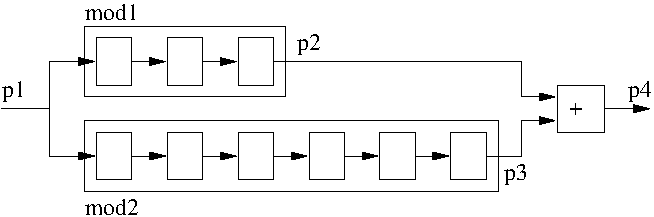
\includegraphics{pqueue}
        \caption{alternate pipeline paths}
        \label{fig:pqueue}
        \end{figure}
        Here the first shorter path will fill queue \var{q2} after 5 clock cycles (
        assuming \var{q1} is always available). The last statement cannot execute
        because \var{q3} is not yet available, the second pipeline path being longer.
        The buffer in q2 is now full so it becomes unavailable for writing and the same
        will apply through the first pipeline. But this means that the first pipeline
        will stop reading \var{q1} which means that the second branch has not yet
        reached the output but cannot continue to read \var{q1}. The data already in
        the second pipeline will continue to move through the queue but no more input to
        that queue will occur. When the data in the second pipeline reaches the output
        the last assignment statement can now execute until it exhausts the second
        pipeline. The two pipeline branches are interacting and this will slow
        throughput to about half. This interaction can be eliminated by making the queue
        buffer depth of queue \var{q2} large enough to keep accepting data until the
        second pipeline fills. The example would be fixed by -
        \begin{lstlisting}[language=threepl]
            queue({q1, q2, q3, p4}, "uint:8");
            attributes(q2, depth=16);

            mod1(q2 <- q1); // assume this module has 3 pipeline stages
            mod2(q3 <- q1); // assume this module has 6 pipeline stages
            p4 <<- q2 + q3;      
        \end{lstlisting}
        The buffer size is rounded up to various powers of two. Which powers of
        two, and the maximum allowed, depend on the FPGA - see the 3PL manual.




    \section{Target exceptions}

        3PL is designed for the generation of code which will process continuous
        data streams. If an exception condition arises it may prove necessary to
        prematurely exit from a conditional or loop block. In particular a
        statement within a block may be waiting for queue availability where
        the exception condition is such that this will not occur. A way is
        needed to force an exit from loops, code blocks or blocked statements.

        The following target constructs may have an {\bf unless} clause attached -
        \blist
        \item   {\bf seq \{\}}
        \item   {\bf par \{\}}
        \item   {\bf sync \{\}}
        \item   {\bf when ()}
        \item   {\bf when () else}
        \item   {\bf seq while () \{\}}
        \item   {\bf par while () \{\}}
        \item   {\bf sync while () \{\}}
        \item   {\bf seq do \{\} while ();}
        \item   {\bf par do \{\} while ();}
        \item   {\bf sync do \{\} while ();}
        \blend

        For example a seq block may have some queue reads which we want to terminate
        when an exception condition occurs -
        \begin{lstlisting}[language=threepl]
            static({s1, s2}, ...);
            queue({q1, q2}, ...);
            value(e, "log", ...);

            seq {
                s1 <- q1;
                s2 <- q2;
            } unless (e)
        \end{lstlisting}
        The {\bf seq} is at the top level and will execute in an infinite loop. If
        \var{e} is true the {\bf seq} will immediately terminate on the next clock
        edge. If any assignments in the {\bf seq} were ready to execute on that clock
        edge they will do so. Following termination the normal sequence of execution of
        the thread will continue, in this case the {\bf seq} immediately executing
        again. This is probably not what we want - there is usually some corrective
        code we wish to execute. To do this  there is an optional execution block
        associated with the {\bf unless}, e.g. -
        \begin{lstlisting}[language=threepl]
            static({s1, s2}, ...);
            queue({q1, q2}, ...);
            value(e, "log", ...);

            seq {
                s1 <- q1;
                s2 <- q2;
            } unless (e) {
                reset(q1, q2);
            }
        \end{lstlisting}
        The exception code body is in braces and may contain a number of statements,
        however it can only contain one target statement. That target statement
        may of course be a {\bf seq \{\}}, {\bf when ()},  {\bf par while () \{\}} etc.
        The exception code block is executed after the terminated block, following
        which normal thread execution will continue.

        Target statements with {\bf unless} clauses cannot be nested\footnote{Nesting
        of target statements with {\bf unless} clauses may be allowed in the future
        if and when I can figure out the complicated logic to do it.}.


    \section{combinatorial output memory}

        Combinatorial output memory can be used as a combinatorial function on read,
        i.e. when an address is present at the input the memory output will reflect
        the value stored at that address after a short delay. A memory read does not
        require a clock. A memory write is clocked. In the case of Xilinx FPGAs
        combinatorial output memory is distributed CLB RAM.

        Combinatorial output memory is accessed by means of variables whose mode
        is \kwd{cmemory}. These can only be created by the inbuilt procedure
        \kwd{cmemory()}, e.g.
        \begin{lstlisting}[language=threepl]
            int(ports, 2);
            str(dtype, "uint:8");
            str(atype, "uint:6");
            var(init, "[]uint", {.., .., .., .., ..    , ..});
            cmemory(m1, ports, atype, dtype, init);
        \end{lstlisting}
        The first argument to \kwd{cmemory()} is the identifier for the created
        variable. The second argument is the number of ports which for Xilinx
        can be 1 or 2. The address type and data type follow. These can be any type
        at all but the address type is restricted to a maximum width of 9 bits.
        The last argument is initialisation data for the memory and is optional.
        The initialisation argument is shown in the example as an array variable
        but it could be a list of values in braces. Where an array variable is
        used it could of course contain values computed in an immediate execution
        loop, e.g. values implementing a mathematical function or a translation table.

        If the memory has more than one port the ports can be accessed independently.
        In the case of Xilinx the second port, port 1, is read-only. The ports can
        be accessed at multiple places in the code but the code must be written
        to ensure that access on a port is mutually exclusive as access conflicts are
        not detected or resolved.

        Because the memory behaves as a combinatorial element on reading, the memory
        output is accessed via an inbuilt function, e.g.
        \begin{lstlisting}[language=threepl]
            static(d, dtype);
            static(a, atype);
            static(l, "log");

            when (l)
                d <- cmemoryread(m1, 0, a) + 3;
        \end{lstlisting}
        The memory data is available in the same clock cycle that the read occurs
        because it does not have to wait for a clock - the address propagates through
        the memory emerging as the stored data element at the output.

        This example uses static variables. When \var{l} is true \var{d} is
        assigned the sum of the memory output from port 0 at address \var{a} and
        the constant 3. We could also use queue variables, e.g.
        \pagebreak
        \begin{lstlisting}[language=threepl]
            float(gamma, 0.45);
            float(gain, pow(256.0, 1.0 - 1.0 / gamma));
            str(dtype, "uint:8");
            var(init, "[256]uint");
            for (int(i) ; i<256 ; i++)
                init[i] = round(gain * pow((float)i, 1.0 / gamma));
            cmemory(gamma_correct, 1, dtype, dtype, init);
            queue({q1, q2}, dtype);

            .
            .
            q2 <<- cmemoryread(gamma_correct, 0, q1);
            .
            .
        \end{lstlisting}
        where the memory read occurs whenever queues \var{q1} and \var{q2} are
        available (writing of \var{q1} and reading of \var{q2} are not shown in
        the code fragment). This example purports to show an 8-bit pixel gamma
        correction (I may have the function wrong, but you get the idea). The
        gamma correction lookup table is a cmemory mode variable with one port.
        The address input and data output are each 8 bits wide. The initialisation
        array has its contents computed during immediate execution using the
        value initially assigned to floating point variable \var{gamma}. The
        floating point values are rounded back to the nearest integer for
        assignment to the initialisation array\footnote{3PL provides
        target floating point format but arithmetic operations are logic-intensive and
        must be pipelined, i.e. FP operations cannot be done in one step in one
        clock cycle. There is a library of pipelined floating point operations.}.
        A variation is to use a two-port cmemory and allow table entries to be
        overwritten from an external CPU when required. The ZYNQ platform and
        various boards with a serial interface provide this facility and the
        above code might then be written as -
        \begin{lstlisting}[language=threepl]
            class(cpu, cpu_api());
            str(dtype, "uint:8");
            cmemory(gamma_correct, 2, dtype, dtype); // 2 ports, separate for read and write
            queue({wdata, waddr, q1, q2}, dtype);
            cpu.write_queue(wdata <- 1);
            cpu.write_queue(waddr<- 2);

            cmemorywrite(gamma_correct, 0, waddr, wdata);

            .
            .
            q2 <<- cmemoryread(gamma_correct, 1, q1);
            .
            .
        \end{lstlisting}
        The library module \kwd{cpu\_write\_queue()} allows a CPU coupled to the FPGA
        to write to a queue variable in the FPGA. The input arguments \var{1} and
        \var{2} are memory-mapped bus addresses for the bus interface to the FPGA.
        In this example the \kwd{cmemorywrite()} inbuilt procedure will write to the
        memory when queues \kwd{waddr} and \kwd{wdata} are both available.

        Of course we could combine a more complicated execution thread
        with queue variables -
        \pagebreak
        \begin{lstlisting}[language=threepl]
            struct(s,
                sum,    "uint:16",
                count,  "uint:16"
            );
            queue(dp, s);
            queue(ap, atype);
            static(count, "uint:16");
            static(accum, "uint:16");

            seq {
                sync while (ap != 0) {
                    accum <- accum + cmemoryread(m1, 0, ap);
                    count++;
                }
                sync {
                    dp.sum <<- accum;
                    dp.count <<- count;
                    count <- 0;
                    accum <- 0;
                }
            }
        \end{lstlisting}
        Here we loop reading memory and accumulating the sums of the values until
        the queued address is zero, at which point the sum and count are written
        to a queue (whose type is a struct containing fields for both values) and
        the static variables are cleared for the next iteration. The seq block then
        repeats.

        In this last example if the input queue \var{ap} transmits all zeros the
        output data stream \var{dp} will be at the same rate, otherwise the output
        will be at a lower rate which depends on the length of non-zero sequences.
        This is a characteristic of a systolic network with buffered queues, compared
        with a normal signal processing lock-step approach, that each datum can
        proceed through the network at a rate determined by producers and consumers
        at each node of the network. Where all inputs to the network have data available
        and each node can execute in one clock cycle then data can flow at clock rate.
        Where data input is sporadic or at sub-clock-rate, or multiple sequential
        execution cycles are needed at some nodes, the data throughput will be slower.




    \section{registered output memory}

        Registered output memory uses a clock for both read and write. On executing a
        read the data appears at the output following the next clock edge. In the case
        of Xilinx FPGAs registered output memory is block RAM.

        Because the memory output is delayed one clock cycle on a read, registered
        output memory reads must be pipelined, otherwise a read will take two clock
        cycles.

        Registered output memory is accessed by means of variables whose mode
        is \kwd{rmemory}. These can only be created by the inbuilt procedure
        \kwd{rmemory()}.

        In the previous section we had an example where data bytes were streamed
        through a look-up table for gamma correction -
        \begin{lstlisting}[language=threepl]
            type(dtype, "uint:8");
            cmemory(gamma_correct, 2, dtype, dtype);
            queue({wdata, waddr, q1, q2}, dtype);

            .
            .
            q2 <<- cmemoryread(gamma_correct, 1, q1);
            .
            .
        \end{lstlisting}
        We could convert that example to use registered output memory as follows -
        \begin{lstlisting}[language=threepl]
            type(dtype, "uint:8");
            rmemory(gamma_correct, 2, dtype, dtype);
            queue({wdata, waddr, q1, q2}, dtype);

            .
            .
            seq {
                rmemoryread(gamma_correct, 1, q1);
                q2 <<- rmemoryout(gamma_correct, 1);
            }
            .
            .
        \end{lstlisting}
        The seq loop will first attempt to execute a memory read from port 1 taking
        the address from queue \var{q1}. If \var{q1} is not available then the read
        will wait until it is. When the read has occurred the seq block will then
        execute the assignment of the current output value of the memory to queue
        \var{q2} (if \var{q2} is not available it will wait). The inbuilt function
        \kwd{rmemoryout()} gets the contents of the output register of the block RAM
        for the specified port. This value will remain in the output register until
        another memory read is executed. This code example does not pipeline the
        memory reads and hence takes two cycles per access.

        Note that in this example \kwd{rmemoryread()} is a procedure, not a module,
        so the module in which \var{q1} is being read is the file module.
        Since there is only one sink for queue \var{q1} we do not need to worry
        about ensuring that bits of the code are in separate modules and hence
        all the code is in the file module. If queue \var{q1} was also
        read by other unrelated code we would have to ensure that the reads were
        in separate modules so that the independent reads were handled correctly.

        To pipeline the above example the memory read must be separated from the
        following memory output value assignment. The assignment is dependent on
        a previous memory read so we need to signal that this has occurred. This
        could be done with another queue variable -
        \begin{lstlisting}[language=threepl]
            type(dtype, "uint:8");
            rmemory(gamma_correct, 2, dtype, dtype);
            queue({wdata, waddr, q1, q2}, dtype);
            queue(read, "log");

            .
            .
            sync {
                rmemoryread(gamma_correct, 1, q1);
                read <<- true;
            }

            when (read)
                q2 <<- rmemoryout(gamma_correct, 1);
            .
            .
        \end{lstlisting}
        but this code is not correct! If queue \var{q2} becomes unavailable for
        writing the assignment to it will wait but the next memory read may go
        ahead, overwriting the previous registered memory output value. We could
        acknowledge back via another queue but that would introduce an extra clock
        cycle.

        We need to execute the memory read and assign the result in the one clock.
        Since the read must occur in a clock cycle previous to the assignment to q2
        the two operations can be staggered by doing an initial read prior to
        entering the loop.
        \pagebreak
        \begin{lstlisting}[language=threepl]
            type(dtype, "uint:8");
            rmemory(gamma_correct, 2, dtype, dtype);
            queue({wdata, waddr, q1, q2}, dtype);

            .
            .
            seq {
                rmemoryread(gamma_correct, 1, q1);
                sync {
                    q2 <<- rmemoryout(gamma_correct, 1);
                    rmemoryread(gamma_correct, 1, q1);
                }
            }
            .
            .
        \end{lstlisting}
        here -
        \blist
        \item   the first statement in the {\bf seq} block executes the first read
        \item   the second statement in the {\bf seq} is an infinite loop
        \item   the loop sync block will not execute until {\bf q1} and {\bf q2} are
                available ({\bf q1} is not empty and {\bf q2} is not full)
        \item   {\bf q2} is assigned the previous result and the next read are performed
                simultaneously
        \item   the {\bf seq} block never completes
        \blend

        ANother approach is to create a module to handle pipelined
        rmemory reads -
        \begin{lstlisting}[language=threepl]
            type(dtype, "uint:8");
            rmemory(gamma_correct, 2, dtype, dtype);
            queue({wdata, waddr, q1, q2}, dtype);
            queue(read, "log");

            .
            .
            rread(q2 <- gamma_correct, 1, q1);
            .
            .
        \end{lstlisting}
        The code for the module might be -
        \begin{lstlisting}[language=threepl]
            global module
            rread (queue(data) <- rmemory(m), int(port), queue(addr)) {
                static(hold, "log");
                when (!hold || >data)
                    rmemoryread(m, port, addr);
                when (hold)
                    data <<- cast(rmemoryout(m, port), type(data));
                hold <- <addr || hold && !>data;
            }
        \end{lstlisting}
        We have declared the module as \kwd{global} so that it can be used anywhere -
        the scope of variables, modules, procedures and functions is discussed in
        a later section. In this module a static boolean variable \var{hold} is used
        to synchronise the memory reads and output queue assignments. When \var{hold}
        is true a value is held in the memory output register waiting to be assigned
        to the output queue. There are three statements in this module, each one
        executing independently in its own implicit infinite loop.

        The first statement executes a memory read if the hold flag is false (there
        is currently no unassigned registered memory output value) or if the output
        queue is available for writing (the {\bf \verb'>'} unary prefix operator returns
        true if the queue variable to which it is applied is available for writing -
        there is a similar operator, {\bf \verb'<'} for read availability). If
        {\bf \verb'<'}q1 is not true the statement will wait until it is true.

        The second statement assigns the registered memory output value to the output
        queue when \var{hold} is true. If the output queue \var{data} is not available
        this statement will wait untli it is available then execute the write.

        The third statement continually updates the value of \var{hold} - it is
        assigned true if an input is available or it is already true and the output
        queue is not available, otherwise it is assigned false.

        This module is already included in a 3PL library.


    \section{Clocks}

        A clock is another mode of variable - mode \kwd{clock}. A Clock variable can
        represent -
        \blist
        \item   a clock input from an input buffer driven from an FPGA pad
        \item   a clock signal between a digital clock manager and a global
                clock buffer
        \item   a clock signal distributed over a clock net driving FPGA
                synchronous logic 
        \blend

        A clock mode variable is created by calling the inbuilt procedure
        \kwd{clock()}. For an input clock signal various attributes such as
        the frequency and the FPGA pin(s) must be supplied. For example -
        \begin{lstlisting}[language=threepl]
            str(c100_pin, "E17");
            clock(c100, frequency=1.0e8, loc=c100_pin);
        \end{lstlisting}

        If the clock variable does not represent the output of an input clock buffer then
        there is no location attribute.

        If a clock is passed as an argument to a module, procedure or function
        then the parameter is not given any attributes, e.g.
        \begin{lstlisting}[language=threepl]
            procedure
            p (.... <- clock(c)) {
                .
                .
            }
        \end{lstlisting}

        To generate a clock a digital clock manager (DCM) is used. The following code
        illustrates this -
        \begin{lstlisting}[language=threepl]
            str(c100_pin, "E17");
            clock(c100_in, frequency=100.0, loc=c100_pin, ibufg=true);
            clock({global.c100, c100_raw});
            clkdcm(clk0=c100_raw <- clkin=c100_in, clkfb=c100);
            clockbuffer(c100 <- c100_raw);
        \end{lstlisting}
        \begin{figure}[htbp]
        \centering
        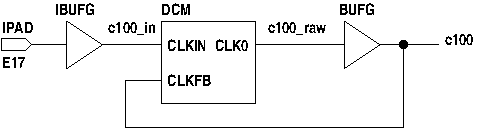
\includegraphics{dcm}
        \caption{digital clock manager}
        \label{fig:dcm}
        \end{figure}
        Creating c100 with global scope ensures that it is globally accessible
        where \kwd{c100\_in} and \kwd{c100\_raw} may have local scope.
        Library procedures \kwd{clkdcm} and \kwd{clockbuffer} both propagate
        the frequency and period attributes from inputs to outputs so we don't
        have to assign these attributes to \kwd{c100\_in} and \kwd{c100\_raw}.

        Before any logic involving synchronous elements is generated by 3PL the
        clock domain must be established. This is done by calling the inbuilt
        procedure \kwd{useclock()}, e.g.
        \begin{lstlisting}[language=threepl]
            useclock(c100);
        \end{lstlisting}

        When the clock domain is changed using \kwd{useclock()} the previous clock domain
        is pushed onto a stack. If \kwd{useclock()} is called with no argument the previous
        clock domain is popped off the stack and again becomes the current clock domain.

        The clock domain used by variables is established when they are assigned
        or evaluated, not when they are created.

        For a static variable the clock domain in use when the variable is assigned
        a value or is evaluated establishes the clock domain for the variable. Any
        other assignments or evaluations of that variable must be in the same clock
        domain.

        For a queue variable the read and write clock domains may be different. The write
        clock domain is established by the clock domain in use when the first write is
        encountered and all subsequent writes must be in the same clock domain. Similarly
        the read clock domain is established by the clock domain in use on the first read
        of the queue and all subsequent reads must be in the same clock domain. If the read
        and write clock domains are the same, which is the usual case, the queue is called
        {\bf synchronous} and the queue buffer depth will be 2 by default. If the read and
        write clock domains differ the queue is called {\bf asynchronous} and the default
        buffer depth is 16. Resynchronisation of queue data between the two clock domains
        is handled automatically by the asynchronous queue.

        In general in a statement the clock domain in use must agree with the clock
        domain of variables that are assigned or evaluated in that statement.
        Procedure and module calls are an exception in that the clock domains are
        checked in the body of the called module or procedure but not when arguments
        are evaluated and passed to parameters.

        The correct way to pass data from one clock domain to another is via an
        asynchronous queue, however there are two functions, \kwd{accept()} and
        \kwd{sample()} which allow mixing of clock domains at the programmer's
        peril. \kwd{accept()} simply overrides the clock checks and can be used if
        data is seldom changed and the risk of data corruption is acceptable (safe
        for single bit data except for the very small probability of getting a
        metastable state. For single bits an inbuilt function \kwd{resync()} can be
        used to do this properly). \kwd{sample()} preserves data integrity by
        resampling it into the current clock domain, however since the clock
        frequencies differ a datum may be lost or duplicated (but will not be
        corrupted).


    \section{Modules}

        Modules and procedures were briefly mentioned in the context of queue variables. A
        module has the important property that it delineates a sink for queue variables.
        When a Queue has more than one sink each sink must execute a read on the queue
        before the datum is popped and the next becomes available. Multiple reads within a
        sink are treated as a single read if they occur simultaneously, otherwise they are
        separate reads. A queue has two sinks if the two code sections which read the queue
        are in different modules, For example -
        \begin{lstlisting}[language=threepl]
        queue({p, q1, q2}, t1);

        .
        p <<- .....;
        m1(q1 <- p);
        m2(q2 <- p);
        .

        module
        m1 (queue(pout) <- queue(pin)) {
            pout <<- p - 3;
        }

        module
        m1 (queue(pout) <- queue(pin)) {
            pout <<- p * 2;
        }
        \end{lstlisting}
        Modules are declared with output parameters followed by input parameters,
        these lists being separated by {\bf \verb'<-'} (the left arrow can be
        omitted if there are no output parameters). Each parameter is a call to
        an inbuilt variable creation procedure. References to parameters in
        the module code body are replaced by the arguments passed in the call.
        If a parameter is not passed an argument then it becomes a local variable.
        For this reason parameters can have initial values which become the
        variable initial values if no matching argument is provided. There is
        an inbuilt procedure {\bf matched()} which can be used to test if a
        parameter has been passed an argument. Arguments are normally matched
        to parameters by the order in which both occur however an alternative
        is to use {\bf parameter=argument} pairs in the call. This is useful
        where there are many parameters and only a few are to be passed arguments.
        A combination of both modes is allowed as long as no positional arguments
        follow any parameter=argument pairs.

        Parameters can have target type widths missing, dimensions missing or
        even a type missing or a mode missing. The missing elements will be filled
        in from the argument. Where parameters have types and dimensions these
        will be checked against the argument type and dimensions. An exception
        is target numeric type widths which allow a mis-match, resulting in truncation
        or padding.

        A module is a block of code which can be called. Module calls are
        only done during immediate execution. There is no code in the FPGA which
        executes any sort of shared code call! When a module is called however
        any target statements that it contains are established as independent
        execution streams. A module call would not usually be made within a target
        construct such as a \var{when} or one of the target loops. In contrast
        a procedure containing a target statement called within a target construct
        will result in that statement appearing in-line where the call is made.

        Declaring a module and calling it can be verbose and inconvenient, especially if
        the code blocks are small and the modules are only called once. Instead an un-named
        module can be used. An un-named module is code enclosed in square brackets. It is
        not called as such but simply appears in-line, though it is executed as a distinct
        and separate module from that within which it is nested. The above code could be
        written
        \begin{lstlisting}[language=threepl]
        queue({p, q1, q2}, t1);

        .
        p <<- .....;
        [q1 <<- p - 3;]
        [q2 <<- p * 2;]
        .
        \end{lstlisting}
        where now the assignments to queues \var{q1} and \var{q2} are in separate
        modules - the code in brackets. Un-named modules do not have calls and hence
        there are no arguments and parameters. The scope of an un-named module is like
        that of a code block in braces. Variables created inside the brackets are in
        the scope of the un-named module. But code within the un-named module can
        access the scope in which it is enclosed - in the case above \var{p}, \var{q1}
        and \var{q2} occur in the scope outside the two un-named modules but are
        accessible within the un-named modules.

        Note that in this example the assignment to \var{q1} will occur when both
        \var{q1} and \var{p} are available. Similarly  the assignment to \var{q2} will
        occur when both \var{q2} and \var{p} are available. If \var{q1} and \var{q2}
        become available at different times the assignments will not occur
        simultaneously, but each will read the same datum from \var{p} since \var{p}
        will not pop its datum until both reads have occurred (the first read to occur
        will not see \var{p} become available again until after the second read has
        occurred). If instead the code was
        \begin{lstlisting}[language=threepl]
        queue({p, q1, q2}, t1);

        .
        p <<- .....;
        q1 <<- p - 3;
        q2 <<- p * 2;
        .
        \end{lstlisting}
        it would function correctly if all three queues were available, both \var{q1}
        and \var{q2} being assigned the datum from \var{p}. If however \var{p} and
        \var{q1} were available but \var{q2} was not, the assignment to \var{q1} would
        take place and the datum would be popped from \var{p}. When \var{q2} became
        available it would read the next datum from \var{p}. Another solution might be 
        \begin{lstlisting}[language=threepl]
        queue({p, q1, q2}, t1);

        .
        p <<- .....;
        sync {
            q1 <<- p - 3);
            q2 <<- p * 2);
        }
        .
        \end{lstlisting}
        which inhibits both assignments until all three queues are available.



    \section{Modules, procedures, functions and classes}

        3PL provides user-defined procedures and functions.

        Briefly -
        \blist
        \item   module, procedure, function and class calls are only executed during
                immediate execution - the calls are not executed in the FPGA
        \item   modules and procedures are called using the same syntax and semantics
        \item   modules and procedures are declared the same way except for the
                keyword {\bf module} or {\bf procedure}
        \item   a module may contain any number of target statements whereas a
                procedure can contain at most a single target statement (but which
                may be a seq, par sync etc.)
        \item   each target statement in a module is established in its own
                execution thread whereas the single target statement in a procedure
                is executed in-line at the location of the call
        \item   modules and procedures with no target statements are functionally
                identical
        \item   modules delineate queue sinks but procedures do not
        \item   functions can only appear within the context of an expression -
                they cannot be called using module or procedure call syntax
        \item   functions can return immediate or target values
        \item   functions cannot contain in-line target statements - they can
                contain module calls
        \item   classes are called in a similar manner to modules or procedures but
                they return a value, a class instance
        \item   a class cannot contain in-line target statements
        \blend

        A procedure call and definition are illustrated by the following example -
        \begin{lstlisting}[language=threepl]
            static(s, "uint:8");    // unsigned integer of 8 bits
            static(v, "[2]uint:8"); // array of 2 unsigned integers of 8 bits

            p(s <- v[0], v[1] + 2, 3);

            procedure
            p (static(os, "int:8") <- value({iv1, iv2}, "int:8"), int(i)) {
                os <- iv1 + (iv2 >> i);
            }
        \end{lstlisting}
        This procedure, \var{p}, has one output parameter, the 8-bit integer
        static mode variable \var{os}, and three input parameters, two
        value variables and an immediate integer variable. Parameters are created
        by using the same variable creation procedures as before.

        procedures have their own variable scope so any variables created in the
        body of the procedure (and any unmatched parameters) are in the local
        scope of the procedure and cannot be accessed from outside the procedure,
        including any deeper calls to procedures (or functions).

        The convention for both procedure definitions and calls is that parameter and
        argument lists consist of outputs, \verb'<-' and then inputs. If there are no
        output parameters in the definition the \verb'<-' can be omitted. Similarly if
        there are no output arguments in the call the \verb'<-' can be omitted. For
        value and immediate mode input parameters the argument is copied to the
        parameter by assignment, i.e. it is call-by-value. For other input parameter
        modes and for all output parameters the parameter 'points' indirectly to the
        argument variable, i.e. call-by reference.

        A value mode input parameter can be passed an argument which is an expression,
        and that expression could be immediate mode (i.e. a constant in the target).
        Similarly an immediate mode input parameter can be passed an argument which
        is an expression, however that expression must be immediate mode, not a
        target mode. In the example above the first input parameter is value mode
        and has been passed one member of a static mode array. The second value
        mode parameter has been passed an expression which is the sum of a
        member of a static mode array and a constant. The body of the procedure
        adds the first parameter to the second parameter right shifted by the
        third and assigns the result to the output static variable.

        For the other cases these are call-by-reference and any reference to the
        parameter accesses the actual variable passed as an argument. Note that
        where the type is an array the argument may be a sub-array,
        e.g. -
        \begin{lstlisting}[language=threepl]
            static(v, "[6]uint:8");

            p(v[1..3]);

            procedure
            p (static(p, "[3]int:8")) {
                ...
            }
        \end{lstlisting}
        This applies to call-by-value and call-by -reference and to both input and
        output parameters.

        If parameter dimensions are given the argument dimensions must be the same,
        however we could omit the parameter dimensions to make the procedure more
        flexible -
        \begin{lstlisting}[language=threepl]
            static(v, "[6]uint:8");

            p(v[1..3]);

            procedure
            p (static(p, "[]int:8")) {
                println(dimensions(p));     // print the number of dimensions of p
                println(dimension(p, 0));   // print the first dimension of p
            }
        \end{lstlisting}
        which would print
        \begin{lstlisting}[language=threepl]
            1
            3
        \end{lstlisting}

        Arguments may be omitted in which case the unmatched parameters become
        local variables in the procedure. Input parameters may be given initial values
        so that these values will be used if no matching argument is passed.

        Arguments are assigned to parameters in left to right order with inputs
        assigned before outputs. This means that when a parameter is created
        the type argument to the inbuilt variable creation procedure could use
        values passed to parameters to the left.

        A parameter can be tested to determine if an argument has been passed to it by
        means of the inbuilt function \kwd{matched()} which returns true if an argument
        has been passed.

        In addition to the usual matching of arguments to parameters by position
        the keymatch format may be used where each argument is identifier=value,
        the identifier being that of the parameter. The keymatch arguments can be
        in any order but arguments are assigned to parameters in parameter order.
        Positional arguments can precede keymatch arguments but cannot follow them.

        Considerable flexibility is allowed in argument passing. Missing parameter
        dimensions can be inferred from the argument dimensions and target type widths
        need not be the same (truncation or padding will result if not).

        Procedures may contain immediate statements however they may only contain at
        most a single in-line\footnote{This qualification will be explained later.}
        target statement! This statement may be a control structure containing other
        target statements nested to any depth. The following procedure definition -
        \pagebreak
        \begin{lstlisting}[language=threepl]
            procedure
            p () {
                a <- 3; //
                b <- 4; // ILLEGAL!
            }
        \end{lstlisting}
        is not allowed. It is not clear what is to be done with two target statements.
        If \var{p()} is called at the top level you might expect the assignments to be
        placed in their own infinite loops. If called in a par{} or seq{} block then
        perhaps they are added to the block. To avoid this uncertainty procedures
        can only contain one target statement but of course this can be a
        \kwd{par\{\}}, \kwd{seq\{\}}, \kwd{when}, \kwd{seq while}, \kwd{par while} etc.

        Functions differ from procedures in that -
        \blist
        \item   there are no output parameters
        \item   there are no in-line target statements
        \item   a function call appears where a value is required, not on
                a line by itself as for a procedure call.
        \item   there is a return statement to return a value - this can only
                be immediate mode or value mode
        \blend

        Functions have local variable scope in the same way as procedures.

        Functions cannot have target statements but they can have target
        expressions and return values. The following illustrates a trivial
        function returning a target mode value -
        \begin{lstlisting}[language=threepl]
            function
            add (value({a, b}, "int:8")) {
                value(v, "int:9")
                v := a + b;
                return(v);
            }
        \end{lstlisting}
        Note that the declaration does not define the return type, so a function
        could have several different return types governed by conditional
        statements.

        The trivial example above is verbose and could be recoded as -
        \begin{lstlisting}[language=threepl]
            function
            add (value({a, b}, "int:8")) {
                value(v, "int:9", a + b)
                return(v);
            }
        \end{lstlisting}
        or simply -
        \begin{lstlisting}[language=threepl]
            function
            add (value({a, b}, "int:8")) {
                return(a + b);
            }
        \end{lstlisting}

        It was previously stated that procedures could contain at most one in-line
        target statement and functions could not contain any. The term "in-line"
        excludes statements contained in modules within a procedure or functions. The
        reason is that a module is an independent block of code that originates target
        execution threads. If a procedure contains a target statement that statement is
        in-line, i.e. that statement will be inserted into the target execution thread
        in the context where the procedure is called. When a module is called it
        establishes a completely new context for establishing execution threads
        unrelated to the context in which it is called. As an example suppose we wish
        to write a function which returns a value which is the value of the argument
        delayed by a number of clock cycles. The function cannot contain target
        statements so it seems that we could not write this, but a function can contain
        a module which in turn can contain target statements. We could write the
        function as follows -
        \pagebreak
        \begin{lstlisting}[language=threepl]
        global function
        del (value(in), int(n, 1)) {
            type(t, type(in));
            static(d, "["+n+"]t");

            [
                d[0] <- in;
                for (int(i, 1) ; i<n ; i++) // loop for i from 1 to n-1
                    d[i] <- d[i-1];
            ]

            return(d[n-1]);
        }
        \end{lstlisting}
        The first input parameter has no type specified so it will use the type of its
        argument. The second argument is immediate and is the delay count. It is set to
        default to 1 if it is not given an argument. Note that the array type is
        constructed as a string expression to insert the dimension gained from the
        second parameter. The value returned for the function is value mode and is the
        value of the last member of the static variable array. Note that the loop
        starts at index 1 as the loop variable \var{i} is initialised to 1.

        The un-named module can access the scope of the function in which it is
        contained. Note that the assignments to variable \var{d} are not in a par
        block. Since we are at the top level of a module each assignment statement will
        execute in parallel in its own infinite loop at clock rate\footnote{The code
        generator will eliminate the loop and simply control the enables to the
        register flip-flops. How and when these are asserted depends on how execution
        in the FPGA is started. It can be started by an external signal or it can start
        spontaneously after configuration - see target-execution-start in the manual
        index. A static variable can have its 'continuous' attribute set to true in
        which case the enables will be tied high.}.

        Procedure and function calls can be recursive. This is a very powerful
        mechanism allowing very simple and concise code to be written. Recursion
        often offers solutions that cannot be written iteratively. Any target code
        is duplicated on each call.

        We could instead write the above example recursively -    
        \begin{lstlisting}[language=threepl]
        global function
        del (value(in), int(n, 1)) {
            if (n == 0)
                return(in);
            static(d, type(in));
            [d <- in;]
            return(del(d, n-1));
        }
        \end{lstlisting}
        Each call to the function delays zero or one clock cycles. If the count
        is non-zero it delays the input by one cycle then calls itself with the
        result and a count minus 1. The assignment again is within an un-named
        module but now it is a single statement. There will be {\em n}
        un-named modules created, each with one assignment.

        When writing iterative code note that it can be convenient to
        use a value variable which is re-assigned on every iteration. The following
        function ORs the bits of its argument.
        \begin{lstlisting}[language=threepl]
        global function
        orbits (value(v, "bits:")) {
            int(n, dimension(v));
            value(ret, "log", cast(getbit(v, 0), "log"));
            for (int(i, 1) ; i<n ; i++)
                ret := ret || cast(getbit(v, i), "log")
            return(ret);
        }
        \end{lstlisting}
        The value variable \var{ret} is initially the LSB of the input but each time
        around the loop it is re-assigned the OR of itself and the next successive bit
        from the input. Finally it is returned as the value of the function. Note that
        the function parameter has no data width - this is derived from the
        argument. We could make two changes to this example. First we could generalise
        it so that it would accept any type for the input. Secondly we could
        avoid the use of the library function \var{getbit()} by casting the input
        into an array of "log".
        \begin{lstlisting}[language=threepl]
        global function
        orbits (value(v)) {
            int(n, size(v));
            value(vx,, forcecast(v, "["+n+"]log"));
            value(ret, "log", vx[0]);
            for (int(i, 1) ; i<n ; i++)
                ret := ret || vx[i]
            return(ret);
        }
        \end{lstlisting}
        The library function \var{forcecast()} is a more extreme version of inbuilt
        function \var{cast()}.
        Where a value variable is given an initial value the type argument can be
        omitted since the type can be inferred from the initial value.

        Module, procedure, function and class definitions may be nested, so a function or
        procedure may be defined within another function or procedure and hence can
        only be called by the parent function or procedure. By this means the scope and
        hence accessibility of functions and procedures can be limited and procedure
        and function identifiers can be re-used locally without ambiguity.

        It may be apparent by now that modules, procedures, functions and classes are only
        called during immediate execution - they are not called within target code. There
        is no equivalent to a procedure or function call in the FPGA code. Indeed this
        would not make sense as it implies shared code and sequential access which defeats
        the purpose of using an FPGA for parallel execution. Procedures and functions are
        useful where the same code is needed multiple times, be it immediate code or target
        code, however the procedure and function calls only take place during immediate
        execution.

        Module, procedures, functions and classes accept a "varargs" parameter which will
        match any number of arguments of any type or mode. This must follow normal
        parameters if used.




    \section{program structure and scope}

        There are a number of variable scopes -

        \blist
        \item   global scope
        \item   file scope
        \item   local scope
        \item   block scope
        \blend

        Global scope is accessible anywhere. Variables are created in global scope if
        the variable identifier has "global." prepended when the variable creation
        inbuilt procedure is called. If the same variable identifier is used in more
        than one scope the global version can be explicitly selected by prepending
        "global.". Variables are never placed in global scope by default.

        When the 3PL compiler begins to compile source code from the source file passed
        to it on the command line it creates a module to contain that code. That module
        is called a {\bf file} module. A file module does not have an identifier since
        it is not explicitly called. Source code within that source file forms the code
        body of the file module and this is executed by the interpreter following
        compilation. Variables created immediately within the file module (i.e. not
        within nested blocks) by default are contained in the file module scope.
        If variables are created within code blocks nested within that file
        scope but their scope is required to be the file scope then their
        identifiers must have "file." prepended. Similarly if necessary a variable
        reference can be disambiguated by prepending "file.".

        3PL allows other source files to be nested within the command line source
        file. There are two mechanisms for doing that.

        A source file can be nested within another by the construction    
        \begin{lstlisting}[language=threepl]
            source "file.3pl"
        \end{lstlisting}
        This simply inserts the text of the file at that point in the current file.
        This can be done to any depth.
        This is equivalent to \#include in C. If instead the code
        \begin{lstlisting}[language=threepl]
            module "file.3pl"
        \end{lstlisting}
        is used the file is inserted as before however a new file module is created
        for which the new source file supplies the code body. again this can be done to
        any depth.

        Any variables created immediately within the new file module are by default
        contained in the file scope for that module. Again this can be made explicit
        by prepending "file." to the variable identifier.

        File scope is useful for hiding variables away from application code without
        the need to call a module for initialisation. For example a hardware
        interface is usually coded as a file module. The source file for this might be
        "gadget.3pl". By including this using the statement
        \begin{lstlisting}[language=threepl]
            module "gadget.3pl"
        \end{lstlisting}
        a file module will be created. Top level code within this file module will
        be interpreted at the point at which occurs in the enclosing source. This
        code will create variable, such as inputs, outputs, FPGA pin names etc. and 
        by default these will be in the file module scope. The module will also
        define modules, procedures and functions which provide the interface to the
        gadget. These can access the variables in file scope but the callers to
        these cannot access the variables. Hiding variables in this way both
        protects the interface from incorrect usage and also avoids accidental
        conflicts with variable identifiers.

        Within a module other than a file module, a procedure or a function variables
        created outside of nested code blocks are by default local to the module,
        procedure or function. They can be accessed anywhere within the module,
        procedure or function but not from any nested calls or from anywhere else.

        Within a code block in braces any created variables are in the scope
        of the block. A problem arises where variables are created conditionally.
        The code
        \begin{lstlisting}[language=threepl]
        procedure
        p (log(l)) {
            if (l)
                int(i);
        }
        \end{lstlisting}
        does what one would expect - creates the integer \var{i} in the scope
        of the enclosing procedure. If this is changed to
        \begin{lstlisting}[language=threepl]
        procedure
        p (log(l)) {
            if (l) {
                int(i);
                float(f);
            }
        }
        \end{lstlisting}
        two variables are created, but they are in the scope of the {\bf if} code
        block in braces, not in the scope of the procedure. To fix this the code
        should be changed to
        procedure
        p (log(l)) {
            if (l) {
                int(local.i);
                float(local.f);
            }
        }
        which creates the variables in the procedure scope.

        Suppose one wishes to write a procedure which creates variables. The code
        \begin{lstlisting}[language=threepl]
        procedure
        myvar (str(name), log(signed)) {
            if (signed)
                static(name->, "int:8");
            else
                static(name->, "uint:8");
        }
        \end{lstlisting}
        will create a variable whose identifier is derived from the string argument
        by using the indirect operator. The problem is that the variable is
        created in the local scope of the procedure, not the scope in which it is
        called. To achieve the latter it can be changed to
        \begin{lstlisting}[language=threepl]
        procedure
        myvar (str(name), log(signed)) {
            str(n, "calling." + name);
            if (signed)
                static(n->, "int:8");
            else
                static(n->, "uint:8");
        }
        \end{lstlisting}
        or more simply
        \begin{lstlisting}[language=threepl]
        procedure
        myvar (str(name), log(signed)) {
            if (signed)
                static(("calling." + name)->, "int:8");
            else
                static(("calling." + name)->, "uint:8");
        }
        \end{lstlisting}
        or even more simply
        \begin{lstlisting}[language=threepl]
        procedure
        myvar (str(name), log(signed)) {
            static(("calling." + name)->, signed ? "int:8" : "uint:8");
        }
        \end{lstlisting}

        When the interpreter encounters a reference to a variable it first searches
        the current code block, then back out through nested code blocks until it
        reaches the local scope of the enclosing module, procedure or function. This
        behaviour is the same  as exhibited by other common programming languages such
        as C or Java. If the variable has not been found the interpreter looks in the
        file (module) scope. Finally it looks in the global scope. If the variable
        identifier has "global.", "file.", "calling." or "local" prepended the
        interpreter explicitly expects to find the variable in the named scope.        

        When a non-inbuilt module, procedure or function is called, the interpreter
        searches from the current local scope back through the scopes of nested module,
        procedure and function {\bf declarations} (NOT calls) until it finds a match.
        If that fails it looks in global scope. Thus, like variables, module, procedure
        and function identifiers can be used in different scopes as long as there is no
        conflict. A module, procedure or function definition occupies the scope of the
        module, procedure or function in which it is defined unless the keyword
        \kwd{global} precedes the \kwd{module}, \kwd{procedure} or \kwd{function}
        keyword, in which case it has global scope, i.e. it can be called from anywhere.

        Nested declarations allow modules, procedures and functions to be limited
        in scope so that they can only be called locally. This also allows
        module, procedure and function identifiers to be re-used locally.





    \section{Selectvalue mode}

        Selectvalue mode creates busses using three-state buffers. A selectvalue
        variable can have a number of conditional assignments. The following is an
        example using this mode -
        \pagebreak
        \begin{lstlisting}[language=threepl]
        selectvalue(bus, "bits:8");
        value(address, "uint:4");
        value(write, "log");
        static(data1, "int:5");
        static(data2, "uint:7");

        when ((address == 3) && write)
            bus |- cast(data1, type(bus));
        when ((address == 7) && write)
            bus |- cast(data2, type(bus));
        \end{lstlisting}
        The assignment operator for a selectvalue is \verb'|-' which is intended
        to look a little like a diagram of a connection to a bus. A conditional
        assignment to an output mode variable uses the same assignment operator
        because again a three-state drive is involved.
        When variable \var{address} is 3 and \var{write} is true, drive \var{data1}
        onto \var{bus}.
        When variable \var{address} is 7 and \var{write} is true, drive \var{data2}
        onto \var{bus}.
        The value of variable \var{bus} can be used in expressions
        the same way as other modes such as value or static.
        It is often the case that a bus must be shared by data of different types.
        This example illustrates this. The bus type has been made {\bf bits} and
        variables \var{data1} and \var{data2} have been cast to that type. In both
        cases the variables have fewer bits than \var{bus} so \var{data2} will be
        zero padded to 8 bits and \var{data1} will be sign extended to 8 bits.



    \section{Priority mode}

        Priority mode creates a priority encoder. The type must be "[]log" where the
        array dimension is at least as large as the number of inputs (it may be larger
        and will be trimmed). The encoder is combinatorial and has the same number of
        outputs as inputs (or one extra, see below). If one or more inputs is true the
        output corresponding to the lowest subscript input which is true will be true,
        all other outputs being false. The following example arbitrates between two
        queue variables which are to be written to a common bus -
        \begin{lstlisting}[language=threepl]
        selectvalue(bus, "uint:8"); // bus
        priority(arb, "[10]log");   // bus arbitration variable
        queue({q1, q2}, "uint:8");   // bus sources

        arb[0] := <q1; // q1 is available for reading
        arb[1] := <q2; // q2 is available for reading

        when (arb[0])
            bus |- q1;
        when (arb[1])
            bus |- q2;
        \end{lstlisting}
        Since the lowest subscript applies to \var{q1} it will have priority
        over \var{q2} if both are available simultaneously. The priority
        variable is dimensioned 10 however the unused higher entries will be
        ignored. One additional output may be used, i.e. \var{arb[2]} in the case of
        the example. This extra output is true if none of the inputs is true.


    \pagebreak
    \section{More on types}

        Target variable types are -

        \begin{tabular}{| l | l |}
        \hline
        bits:{\em n}           & unspecified binary                 \\ \hline
        uint:{\em n}           & unsigned integer                   \\ \hline
        int:{\em n}            & signed integer                     \\ \hline
        log                    & logical                            \\ \hline
        fixed:{\em m} .{\em n} & fixed point                        \\ \hline
        float:{\em m} e{\em n} & floating point                     \\ \hline
                               & enumerated type                    \\ \hline
        null                   & no data                            \\ \hline
        \end{tabular}

        Immediate types are -

        \begin{tabular}{| l | l |}
        \hline
        bits      & unspecified binary                              \\ \hline
        uint      & unsigned integer                                \\ \hline
        int       & signed integer                                  \\ \hline
        log       & logical                                         \\ \hline
        str       & string                                          \\ \hline
        float     & floating point                                  \\ \hline
        \verb'->' & pointer                                         \\ \hline
        type      & type                                            \\ \hline
        list      & a list                                          \\ \hline
        map       & a map                                           \\ \hline
        file      & a file                                          \\ \hline
        empty     & take the type from an initialisation argument   \\ \hline
        \end{tabular}

        In both target and immediate modes the types can be nested within
        arrays or structs. Immediate and target mode types cannot be mixed
        within a struct.


    \section{Inbuilt modules, procedures and functions}

        We have already seen the use of inbuilt procedures such as \var{static()}
        and \var{queue()}. There are very many such inbuilt procedures, even more
        inbuilt functions and a few inbuilt modules. The inbuilt functions include
        the usual numeric and string operations which are for immediate execution only.



    \section{Libraries}

        3PL libraries are source code files that are incorporated into the source
        stream by {\bf source "..."} or {\bf module "..."} statements. It is usual to
        incorporate a library called a {\em header file} as the first line of source
        code. This header file is specific to the FPGA platform and sets up FPGA
        package pins definitions and clock logic and provides interfaces to
        external devices on the platform. There are other libraries which are more
        general and contain useful modules, procedures and functions. Often these
        are already incorporated in the header file.



    \section{Petri nets}

        State machines are a convenient way of expressing a control algorithm. When
        implementing state machines in FPGAs it is usual to represent each state
        by a flip-flop state\footnote{The alternative is to represent the state
        by a counter, which is the usual way in software.}. Exactly one state
        flip-flop should be set at any time. A state transition requires the
        current state flip-flop to be reset and another state flip-flop to be
        simultaneously set. A Petri net is a similar but more general scheme.
        The form of Petri net implemented in 3PL would be described as "a finite
        capacity Petri net with a capacity of 1" which is a less general form.
        Although it is a contradiction in terms one can think of this form of
        Petri net as a state machine implementation where more than one state
        flip-flop can be set at a time. Transitions can then involve some
        flip-flops being cleared and others set. A simple state machine can
        be described by a Petri net.

        In a Petri net we have {\em places} rather than {\em states} and each place
        can have a token (set) or no token (cleared). A transition involves taking
        tokens from one or more places and inserting them in one or more other places.
        Expressions describing when transitions are to take place are called
        {\em predicates}.

        The following is an example of the syntax -
        \begin{lstlisting}[language=threepl]
            petrinet {
                initial q1, q2;
                q1, q2 -> q3, p4 when (a && (b != 0)) {s <- queue1;};
                q3 ->> q1 {l1 <- queue1;};
                q4 -> q2, q3 when (!l2);
            }
        \end{lstlisting}
        Here there are places \var{q1}, \var{q2}, \var{q3} and \var{p4}. Each of these
        is a static variable of type "log". If they have not already been created the
        Petri net construct creates them. These variables cannot be assigned by any
        code, only by the Petri net mechanism itself, however their values can be used
        in the program code outside of the Petri net in the same way that ordinary
        variables are used.

        In the example places \var{q1} and \var{q2} initially have tokens. When the
        expression $a \&\& (b != 0)$ (called the {\em predicate}) is true and \var{q1}
        and \var{q2} both contain tokens (are set), \var{q1} and \var{q2} will have
        their tokens removed (are cleared) and places \var{q3} and \var{p4} have tokens
        inserted (are set). The single right arrow indicates a weak transition, meaning
        that prior to the transition any tokens in the destination places are ignored.
        If a double right arrow is used this signifies a strong transition, meaning
        that the transition can only occur if the destination places do not have
        tokens.

        In the example above the code block to the right of the first transition is
        executed when the transition occurs. It may contain
        only a single target statement (which can of course be a compound statement
        such as  {\bf seq\{\}}, {\bf par\{\}} etc.). If a transition does not have a
        predicate then it occurs when the source places have tokens (and optionally
        destination places lack tokens). A transition code block may contain immediate
        statements but these would serve little purpose as they are only executed as the
        interpretter passes through the code during immediate execution.

        To code a state machine as a Petri net the following apply -
        \blist
        \item   each transition has only one source and one destination place
        \item   only one place is initialised
        \item   transitions can be weak (it doesn't matter which are used, but
                weak transitions use fewer logic resources)
        \blend



\pagebreak

\chapter{Variables, Constants, Types, Modes, Attributes, Operators and Expressions}



    \section{Input format}
    
        \index{input format}
        The source code input may use either UNIX-style (newline character) or
        DOS/Windows-style (carriage return, line feed) line termination. Tokens
        are separated by white space (spaces, horizontal tabs or newlines). Good
        formatting dictates the use of indenting but the compiler treats
        indenting as simply white space. The last source code line need not be
        terminated by a newline character, but it is usually preferable to do
        so.

        \index{comments}
        Comments may have the form "/* ....... */", in which case they
        may run over line breaks, or they may be indicated by "//....."
        where they occupy the rest of the current line.


    \section{File inclusion}\label{sec:fileinclusion}

        Source files may be inserted in-line by means of file inclusion
        statements. These are of two forms.
        
        The first form
        \begin{lstlisting}[gobble=8, language=threepl]
           source "filename"
        \end{lstlisting}
        \index{source statement}
        \index{statement!source}
        simply inserts the contents of the named file into the current file in
        place of the entire {\em source} statement line. A file may only be
        inserted once by a {\em source} statement.
        
        The second form
        \begin{lstlisting}[gobble=8, language=threepl]
           module "filename"
        \end{lstlisting}
        \index{module statement}
        \index{statement!module}
        also inserts the contents of the named file into the current file in
        place of the entire {\em module} statement line, but it differs from a
        {\em source} statement in that the inserted file establishes a new
        static module scope (for scope discussion see "Program source structure"
        \autorefph{chap:progsrcstruct}). A file may only be inserted once by a
        {\em module} statement.

        White space (only) may precede the {\em source} or {\em module} on the
        line and separate it from the quoted file name. The remainder of the line
        following the quoted file name will be ignored. File inclusions using {\em
        source} or {\em module} statements may be nested to any depth.

        The quoted file name may be replaced in either of the above by
        {\bf directive("ident")}, i.e.
        \begin{lstlisting}[gobble=8, language=threepl]
           source directive("key")
        \end{lstlisting}
        or 
        \begin{lstlisting}[gobble=8, language=threepl]
           module directive("key")
        \end{lstlisting}
        where the directive whose key is "key" contains the name of the
        file to be included. Since file inclusion is done during parsing
        the directive must be assigned using {\bf presetdirective()}
        \autorefph{sec:ippresetdirective} or by using the command line option
        -D.
        
        \index{ifdirective}
        The file inclusion may be made conditional by using one of the following
        forms -
        \begin{lstlisting}[gobble=8, language=threepl]
           source ifdirective("key") "ident"
        \end{lstlisting}
        or 
        \begin{lstlisting}[gobble=8, language=threepl]
           module ifdirective("key") "ident"
        \end{lstlisting}
        where the directive "key" will be examined to determine whether to
        include the file "ident". If directive "key" does not exist or
        it has the boolean value {\bf false} the file inclusion will
        be skipped, otherwise the file will be included. Note that if the
        directive is not boolean its existence will suffice, but if
        boolean its value will be used.
        
        The above forms may also use a directive for the file identifier -
        \begin{lstlisting}[gobble=8, language=threepl]
           source ifdirective("key1") directive("key2")
        \end{lstlisting}
        or 
        \begin{lstlisting}[gobble=8, language=threepl]
           module ifdirective("key1") directive("key2")
        \end{lstlisting}
        Here directive "key1" is used as before to determine whether to
        include the file and directive "key2" contains the name of the
        file. The same directive may be used for both purposes, e.g.
        \begin{lstlisting}[gobble=8, language=threepl]
           module ifdirective("lib1") directive("lib1")
        \end{lstlisting}
        will include the file whose name is contained in directive "lib1"
        if that directive is defined.

        File names are used exactly as supplied so any file name extension
        must be included (use of the extension ".3pl" is recommended but not
        required).

        Note that these file inclusions are performed during parsing, not during
        immediate execution, and so placing a {\em source} statement within
        an {\em if} statement does not make the inclusion conditional (and
        is syntactically incorrect).
        
        Files included by either of these mechanisms must contain syntactically
        complete code, i.e. statements cannot be partially contained in an
        included file.
        
        Since there are two mechanisms for inserting files, a file should
        be able to ensure that it is not inserted by the wrong mechanism.
        This can be done by including one of the lines
        \begin{lstlisting}[gobble=8, language=threepl]
           nosource
        \end{lstlisting}
        \index{nosource statement}
        \index{statement!nosource}
        to preclude sourcing this file or
        \begin{lstlisting}[gobble=8, language=threepl]
           nomodule
        \end{lstlisting}
        \index{nomodule statement}
        \index{statement!nomodule}
        to preclude calling this file as a module.
        These must have no leading characters before the keyword. The remainder
        of the line is ignored. 



    \section{Single constants}

        \index{constants}
        Integer constants may be
        \blist
        \item    decimal
        \item    hexadecimal (leading 0x or 0X)
        \item    octal (leading 0)
        \item    binary (leading 0b or 0B).
        \blend
        Their size is 64 bits.

        Logical constants are {\bf true} and {\bf false}.

        Floating point constants are decimal integers with a leading,
        trailing or embedded '.' and an optional exponent consisting of "E"
        or "e", an optional sign followed by an integer. If an exponent is
        supplied the '.' can be omitted where appropriate.

        String constants have double quotes surrounding the string. The string
        may contain escape characters
        \blist
        %\item   \verb'\a' alert (bell)
        %\item   \verb'\e' escape
	\item   \verb'\n' new line (line feed)
        \item   \verb'\t' horizontal tab
        %\item   \verb'\v' vertical tab
        \item   \verb'\b' backspace
        \item   \verb'\r' carriage return
        \item   \verb'\f' form feed
        \item   \verb'\\' backslash
	\item   \verb+\'+ single quote (single quotes do not need to be escaped)
        \item   \verb'\"' double quote
        \item   \verb'\0nnn' octal numeric escape where nnn is the 3 digit octal
                character code
        \item   \verb'\xnn' hexadecimal numeric escape where nn is the 2 digit
                hexadecimal character code
        \blend
        
        \index{mathematical constants}
        The global variables {\bf \verb'math_pi'} and {\bf \verb'math_e'}
        of type {\bf float} are created by the compiler prior to immediate
        execution. These variables contain the values for $\pi$ and $e$ and
        are read-only.

    \section{Compound values}

        \index{compound!value}
        \index{value!compound}
        Compound values are (possibly nested) array or struct values.
        \blist
        \item   They can be used to initialise compound variables.
        \item   They can be assigned to compound variables.
        \item   They can be passed to compound immediate or value
                parameters in modules, procedures or functions.
        \blend

        A compound value is a comma-separated list enclosed in braces. Each list
        element is an immediate expression or a compound value Each set of braces
        matches a top level or nested array or struct. Trailing elements for an
        array or struct may be omitted. Initial or intermediate elements may also
        be omitted, commas being placed to indicate this. Lists must not exceed the
        length of the array or struct they are intended to match.
        
        A compound value is processed from left to right, thus the left-most
        item will appear at the lowest subscript or address.
        
        Missing elements in a compound value are simply not assigned.
        Where a compound value with missing elements is used to initialise
        an immediate compound variable, or is assigned to it, the variable
        elements corresponding to the missing values will simply retain
        their previous or default values. Where a compound value is
        similarly used for a value variable, the variable elements
        corresponding to the missing constants will not be assigned, retaining
        their previous values (none if not previously initialised or assigned).

        Examples -
        \begin{lstlisting}[gobble=8, language=threepl]
           var(i, "[3][2]in", {{1, 2}, , {3}});
           struct(s,
               f1,     "[3]int",
               f2,     "log",
               f3,     "str"
           );
           var(v, s);
           v = {{3, 4, 5}, true, "fred"};
           proc(a <- {7, 8, false});
        \end{lstlisting}
        
        Where a struct is initialised, assigned or passed an argument the
        field values may be specified by naming the fields rather than matching
        values to fields by position as in the example above, e.g.
        \begin{lstlisting}[gobble=8, language=threepl]
           struct(s,
               f1,     "[3]int",
               f2,     "log",
               f3,     "str"
           );
           var(v, s);
           v = {f3="fred", f1={3, 4, 5}, f2=true};
           proc(a <- {7, 8, flag=false});
        \end{lstlisting}
        When a struct is assigned values by name in this way no following
        position-matched values are allowed, for example the following
        is accepted -
        \begin{lstlisting}[gobble=8, language=threepl]
           struct(s,
               f1,     "[3]int",
               f2,     "log",
               f3,     "str"
           );
           var(v, s);
           v = {{3, 4, 5}, f3="fred", f2=true};
        \end{lstlisting}
        but it is incorrect to do -
        \begin{lstlisting}[gobble=8, language=threepl]
           struct(s,
               f1,     "[3]int",
               f2,     "log",
               f3,     "str"
           );
           var(v, s);
           v = {{3, 4, 5}, f2=true, "fred"};
        \end{lstlisting}
        because the last value is matched by position but is preceded by
        a value matched by name. This limitation makes sense in that values
        are matched by position in the list to fields in the struct until
        a match by name is encountered after which point the argument positions
        are no longer aligned with the fields.
        
        \index{array!initialisation}
        \index{array!undimensioned}
        \index{dimensions!missing}
        An array initialised by a compound value may have some dimensions
        omitted, in which case the missing dimensions will be inferred from the
        compound value. Array dimensions cannot be omitted where a variable is
        not a module, procedure or function parameter and is not initialised.
        
        Compound value entries for a string array may be types integer,
        boolean or floating point in which case they will be converted to strings.

        Leaf elements in the compound value must be immediate primitive
        types (which includes pointers).


    \section{Identifiers}

        \index{identifier}
        Identifiers begin with a letter or an underscore and contain any
        number of letters, digits or underscores. Alphabetic case is
        distinguished.

        The following keywords may not be used as identifiers

        \index{keywords}
        \blist
        \item   branch
        \item   break
        \item   case
        \item   class
        \item   conditionelse
        \item   continue
        \item   default
        \item   do
        \item   else
        \item   for
        \item   function
        \item   global
        \item   if
        \item   ifcondition
        \item   leadermodule
        \item   module
        \item   null
        \item   par
        \item   petrinet
        \item   postmodule
        \item   private
        \item   procedure
        \item   return
        \item   seq
        \item   source
        \item   switch
        \item   sync
        \item   trailermodule
        \item   unless
        \item   varargs
        \item   when
        \item   while
        \blend

        Identifiers used for -
        \index{identifier!ambiguity}
        \blist
        \item   variables
        \item   struct fields
        \item   modules and procedures
        \item   functions
        \item   directives
        \blend
        are stored in separate tables and hence the same
        identifier can be used for multiple purposes. However, this practice may
        render the code difficult to read.








    \section{Variables and modes}

        \subsection{variable modes}

            \index{modes}
            There are eleven modes of variable -
            \blist
            \item    {\bf immediate}
            \item    {\bf selectvalue}
            \item    {\bf value}
            \item    {\bf static}
            \item    {\bf queue}
            \item    {\bf priority}
            \item    {\bf input}
            \item    {\bf output}
            \item    {\bf cmemory}
            \item    {\bf rmemory}
            \item    {\bf clock}
            \blend

            Immediate variables only exist during program interpretation.
            Variables in the other ten modes are target variables which
            are active in the FPGA logic.


            \subsubsection{immediate variables}

                \index{immediate!variable}
                \index{variable!immediate}
                \index{mode!immediate}
                Immediate variables do not survive into target code except as
                constants (their current value at that point in the code during
                immediate execution). These variables must not have a width
                declared. Immediate integer variables are 64 bits and floating
                point variables are 64 bit double precision.

            \subsubsection{value variables}

                \index{value!variable}
                \index{variable!value}
                \index{mode!value}
                \index{value mode variables}
                Variables of mode {\bf value} represent the result of
                combinatorial expressions and hence do not have state (storage).
                An expression contains constants, variables and function calls
                joined by operators. An expression could consist of a single
                variable in which case the value variable to which it is assigned
                can be thought of as a pointer to that variable (or rather the
                value of the variable, i.e. its output, since a variable cannot
                be assigned (changed) via a value variable pointing to it).

                The availability (see later) of a value variable depends on any
                queue reads in the expression it represents.

            \subsubsection{selectvalue variables}

                \index{variable!selectvalue}
                \index{mode!selectvalue}
                \index{selectvalue mode variables}
                Variables of mode {\bf selectvalue} represent buses or selectors.

                The availability (see later) of a selectvalue variable depends
                on any queue reads in the equivalent expression.

            \subsubsection{input variables}

                \index{variable!input}
                \index{mode!input}
                \index{input mode variables}
                Variables of mode {\bf input} are external inputs.

                An input variable is always (read) available.

            \subsubsection{output variables}

                \index{variable!output}
                \index{mode!output}
                \index{output mode variables}
                Variables of mode {\bf output} are external outputs.

                An output variable is always (write) available.

            \subsubsection{static variables}

                \index{variable!static}
                \index{static mode variables}
                Variables of mode {\bf static} have state - they are registers.
                They have no associated signaling. They may be global, or local to
                modules, procedures, functions or code blocks. Static
                variables involve no signaling and their state changes are not
                implicitly synchronised with pipeline operations except in as much
                as module code may exercise local control.

                Static variables containing arithmetic types may be any size
                but initialisation or assignment from immediate expressions or
                variables are restricted at the moment to a maximum of 64 bits for
                integer or 52.11 for floating point.

                A static variable is always available.

            \subsubsection{queue variables}

                \index{variable!queue}
                \index{mode!queue}
                \index{queue mode variables}
                Variables declared {\bf queue} are dataflow variables which are
                mainly used as pipeline connections between modules. They have
                associated signaling to indicate their availability for reading,
                examination or writing (assignment). When a datum is written to a
                queue, the datum becomes available at the output of the queue. A
                queue may contain more than one datum, in which case the data will
                be available in the order they were written. In a module the
                written end of a queue is referred to as an {\bf output queue}
                since it is assigned to. The read or examined end of a queue is
                referred to as an {\bf input queue}.

                An input queue is available when it has a datum which can be read
                or examined (a datum which is read is removed from the queue
                whereas a datum which is examined remains in place), i.e. it is
                not empty.

                An output queue is available when it can be written to, i.e. it is
                not full.

                Queue variables containing arithmetic types may be any size but
                initialisation or assignment from immediate expressions or
                variables is limited to a maximum of 64 bits for integer or
                52.11 for floating point.
                
                A queue is 'synchronous' if it is written and read in the same
                clock domain.
                
                A synchronous queue has a default buffer depth of 2. An
                asynchronous queue has a default buffer depth of 16. These
                depths can be explicitly set.
                
                \index{null!queue}
                \index{queue!null}
                A queue may be type "null". This is useful for signalling as
                the queue can be written (null must be assigned) or read
                but no actual data storage is used.

            \subsubsection{cmemory and rmemory variables}

                \index{variable!memory}
                \index{mode!memory}
                \index{memory mode variables}
                Variables of mode {\bf memory} represent RAM elements in the
                FPGA.

                Memory variables can only be accessed via inbuilt procedures and
                functions and hence availability does not apply as they cannot be
                used in expressions or assignment statements.

           \subsubsection{priority variables}\label{priorityvariables}

                \index{variable!priority}
                \index{mode!priority}
                \index{priority mode variables}
                Variables of mode {\bf priority} implement a priority encoder
                and are 
                used for arbitration. The type must be a one dimensional array
                of "log" (if the type is omitted "[20]log" will be used). The
                array members are assigned combinatorial values in the same way
                as value mode variables. However, the resultant values of the
                logical array are not simply the input expressions but are
                arbitrated values, the lowest subscript having highest priority.
                Where one or more input expressions to the priority array are
                true, one and only one array value will be true and that one
                will correspond to the true input with the lowest subscript.

                There is an inbuilt function, {\bf prielse()}, which returns
                the value of the else case, i.e. a value which is true when
                no priority inputs are true.

                The entire array need not be assigned. Unused entries will be
                ignored, but where an entry is evaluated (its output is used)
                it must have an assigned input value. The converse is not
                true - an entry that has been assigned need not be evaluated.
                Assignments need not be done in any particular order. This method
                of usage is designed to allow an array that is larger than
                required to be created after which entries can be
                assigned as immediate execution progresses. At the completion of
                immediate execution a priority encoder will be created in target
                code of a size which matches the entries in the array that have
                actually been used. The avoids prior knowledge of the required
                size of the encoder.
        
                A priority variable array member may be assigned more than once
                but the default behaviour is that the final value assigned prior
                to termination of immediate execution prevails, all other
                previous assignments being lost. This can be changed by setting
                attribute "multiplein" to true in which case all assignments
                will be collected and ORed together on completion of immediate
                execution to form the input to that priority array member.

                {\bf At the moment assignments to priority variables cannot
                contain queue reads. This restriction may be removed later.}

                A priority variable is always available.

            \subsubsection{clock variables}
            
                \index{variable!clock}
                \index{mode!clock}
                \index{clock mode variables}
                Variables of mode {\bf clock} are used to represent signals.
                There may be a number of clocks to which program logic is
                synchronised, but there will also be associated intermediate
                clock signals used to connect together the hardware components
                used to generate these program clocks, such as input buffers,
                delay-locked loops and clock buffers.


        \subsection{variable creation}

            \index{variable!creation}
            Variables are created during immediate execution by means of
            inbuilt procedures. The most general procedure used is {\bf
            var(...)}. This has two to four arguments -
            \begin{lstlisting}[gobble=12, language=threepl]
               var(name, mode, type, init)
            \end{lstlisting}

            {\bf name} is the identifier for the created variable.

            Most variable creation inbuilt procedures allow creation of multiple
            variables of the same type, mode and initial value by replacing the
            {\em name} argument by an identifier list enclosed in braces {\em \{v1,
            v2,\dots\}}.

            \index{variable!mode}
            The {\bf mode} argument is optional and must be one of the keywords
            {\bf immediate}, {\bf value}, {\bf selectvalue}, {\bf static} or
            {\bf queue} - memory or input mode variables must be created by
            other procedures (see below). If the mode argument is omitted the
            mode will be {\bf immediate}.

            \index{variable!type}
            The type argument must be a type-valued expression or a string-valued
            expression describing the type. A type-valued expression can be a
            variable or variable member of type "type", the inbuilt functions {\bf
            type()} or {\bf struct()}, or a user-defined function returning type
            "type".
            
            Type specifications in general and type variables in particular
            are described in a \autorefph{sec:types}.

            \index{variable!initialisation}
            \index{initialisation!variable}
            The final argument to {\bf var()} is optional and is an
            initialisation value. This may take one of three forms -
            \blist
            \item   a single immediate expression of appropriate type for a
                    variable of primitive type
            \item   a variable reference of matching type to the created
                    variable
            \item   a compound value
            \blend
            
            For the first two of the above cases where the mode is immediate the
            type argument may be the string "empty" in which case the variable type
            will be the type of the initialisation argument.
            
            Where initialisation is provided and more than one variable is being
            created (using \{...\}) then all variables will be initialised
            identically.

            Immediate, static and queue variables may be initialised. If they are a
            compound type the initialisation argument will usually be a compound
            value or a compound variable of suitable type, but a compound
            type may be initialised by a single immediate value in which case all
            members of the compound type will be initialised to that single value
            (the members of the compound type must all be the same primitive type
            appropriate to the initialisation value).

            Uninitialised immediate and static variables are automatically
            initialised to 0, 0.0, false or "" as appropriate to the type.

            Queue variables when initialised contain a single datum.
            Uninitialised queues have no value as they are not available.
            Initialised queues have a value and they are available.

            A value mode variable can be initialised, but this does not preclude
            assignment of one or more other values later. A value mode variable can
            be initialised with an immediate constant in which case it behaves as a
            target constant unless assigned another expression. Uninitialised value
            variables have no default value. If the value variable is a compound
            type it may be initialised by a compound value.

            Selectvalue variables cannot be initialised but their output when
            no input is selected can be specified.

            Examples of variable creation -
            \begin{lstlisting}[gobble=12, language=threepl]
               var(byte, "int", 8);
               var(sum, value, "uint:16");
               var(even, static, "log");
               var(pixel, queue, "uint:" + byte);
               var(trigger, queue, "null");
            \end{lstlisting}

            The first has no mode declared, so is immediate. It is given an
            initial value of 8. The remainder are target variables. The
            second last example uses the '+' operator to concatenate an
            integer to a string to form the word size. The final example is a
            queue with no data which can be used as an event trigger.
            These examples all use string-valued expressions for the
            type argument. The following examples illustrate the use of
            type-valued arguments -
            \begin{lstlisting}[gobble=12, language=threepl]
               var(t1, type, "int:8");
               var(v1, value, t1);
               var(s2, static, type(v1));
               var(t2, type, type(s2));
               var(q1, queue, "[4]t2");
               var(s3, static, "(f1, int:8, f2, [4]t1)");
            \end{lstlisting}

            \index{mode!immediate!creation}
            \index{variable!immediate!creation}
            For convenience the following procedures can be used instead of
            {\bf var(...)} to create primitive immediate variables -
            \begin{lstlisting}[gobble=12, language=threepl]
               int(name, init);
               log(name, init);
               str(name, init);
               file(name, init);
               type(name, typespec);
               struct(name, field1, type1, field2, type2, .....);
            \end{lstlisting}
            In each case a single variable of the type described by the
            procedure name is created. The initialisation arguments are optional.

            These are further desribed in 
            \blist
            \item   {\bf int()} (\autorefph{sec:ipint})
            \item   {\bf log()} (\autorefph{sec:iplog})
            \item   {\bf str()} (\autorefph{sec:ipstr})
            \item   {\bf file()} (\autorefph{sec:ipfile})
            \item   {\bf type()} (\autorefph{sec:iptype})
            \item   {\bf struct()} (\autorefph{sec:ipstruct})
            \blend

            \index{mode!target!creation}
            \index{variable!target!creation}
            Similarly target variables can be created by-
            \begin{lstlisting}[gobble=12, language=threepl]
                   static(name, type, init);
                   value(name, type, init);
                   queue(name, type, init);
            \end{lstlisting}
            which are equivalent to -
            \begin{lstlisting}[gobble=12, language=threepl]
               var(name, static, type, init);
               var(name, value, type, init);
               var(name, queue, type, init);
            \end{lstlisting}
            In all the above {\em init} is optional.

            These are further desribed in 
            \blist
            \item   {\bf static()} (\autorefph{sec:ipstatic})
            \item   {\bf value()} (\autorefph{sec:ipvalue})
            \item   {\bf queue()} (\autorefph{sec:ipqueue})
            \blend

            \index{mode!memory!creation}
            \index{variable!memory!creation}
            Memory variables are created by the inbuilt procedures -
            \begin{lstlisting}[gobble=12, language=threepl]
               cmemory(name, ports, atype, dtype, init);
               rmemory(name, ports, atype, dtype, init);
            \end{lstlisting}
            These create combinatorial output RAM (mode {\bf cmemory}) and
            registered output RAM (mode {\bf rmemory}) respectively. {\em name} is
            an identifier for the memory, {\em ports} is the number of ports, {\em
            dtype} is the data type, {\em atype} is the address type and {\em init}
            is an optional initialisation array (immediate array variable or
            compound value).
            
            See {\bf cmemory()} (\autorefph{sec:ipcmemory}) and
            {\bf rmemory()} (\autorefph{sec:iprmemory}),
                        
            \index{mode!clock!creation}
            \index{variable!clock!creation}
            Clock variables are created by the inbuilt procedure -
             \begin{lstlisting}[gobble=12, language=threepl]
                clock(name, ...attributes...);
            \end{lstlisting}
            
            See {\bf clock()} (\autorefph{sec:ipclock}).
           
            \index{mode!input!creation}
            \index{variable!input!creation}
            Input variables are created by the inbuilt procedure -
            \begin{lstlisting}[gobble=12, language=threepl]
               input(name, type, ...attributes...);
            \end{lstlisting}
            {\em name} is an identifier for the input variable.
            {\em type} is the variable type.
            {\em attributes} is optional and is either one or more key=value
            attribute arguments or a map of attributes.These arguments can be
            omitted and attributes added later by using inbuilt procedure {\bf
            attributes()}.
            
            See {\bf input()} (\autorefph{sec:ipinput}).
            
            \index{mode!output!creation}
            \index{variable!output!creation}
            Output variables are created by the inbuilt procedure -
            \begin{lstlisting}[gobble=12, language=threepl]
               output(name, type, source, attributes);
            \end{lstlisting}
            {\em name} is an optional identifier for the output variable.
            {\em type} is the variable type (also optional).
            {\bf source} is an optional source value for unconditional assignment.
            {\em attributes} is an optional map of attributes. The argument
            can be a map containing the attributes or can be a compound value
            containing the attributes as key=value entries in one-dimensional
            list. This argument can be omitted an attributes added later by
            using inbuilt procedure {\bf attributes()}.
            
            See {\bf output()} (\autorefph{sec:ipoutput}).
            
            \index{variable!scope}
            \index{scope!variable}
            Variables are normally created within the scope containing the call
            to the variable creation inbuilt procedure. However, if the variable
            identifier has a leading "global.", "file.", "calling." or "local."
            it is created in the specified scope.

            Using "global.", global variables can be created from within any
            scope.

            Using "file.", variables can be created in the current (deepest)
            file module scope.
           
            Using "local." allows the conditional creation of variables in
            the scope of a module, procedure or function. For example the
            code -
            \begin{lstlisting}[gobble=12, language=threepl]
               module
               m (...) {
                   if (doit)
                       static(s, "log");
               }
            \end{lstlisting}
            will create static variable {\bf s} in the module if variable
            {\bf doit} is true. However, the following code -
            \begin{lstlisting}[gobble=12, language=threepl]
               module
               m (...) {
                   if (doit) {
                       static(s, "log");
                       int(j);
                   }
               }
            \end{lstlisting}
            creates variables {\bf s} and {\bf j} in the scope of the
            {\bf if} block and not in the module scope. By changing
            the code to -
            \begin{lstlisting}[gobble=12, language=threepl]
               module
               m (...) {
                   if (doit) {
                       static(local.s, "log");
                       int(local.j);
                   }
               }
            \end{lstlisting}
            variables {\bf s} and {\bf j} are created in the scope of
            the called module.
            
            Using "calling." allows the creation of variables in
            the scope of the previous module, procedure or function.
            This is useful for writing procedures to create variables, in
            which case the created variable needs to be in the calling
            scope, not the scope of the called procedure.

            Variables may be created at any point in the code, but they
            must have been created prior to being referenced.

            A variable reference where the identifier has a scope prepended
            will attempt to locate the variable only in that scope.

            It is important to note that variables exist independently of the
            scope in which they are created. The scope only contains the map
            which ties the variable identifier to the variable, not the
            variable itself. That map disappears with the scope. If a pointer
            to a variable is kept then that variable can be referred to via
            the pointer even though the scope in which the variable was
            created has disappeared. For example the following code illustrates
            a variable created within a function which returns a pointer to that
            variable so that it can be used elsewhere -
            \begin{lstlisting}[gobble=12, language=threepl]
               var(p, "->");
               p = make_static("uint:12");

               when (l)
                   p-> <- v;

               function
               make_static (str(t)) {
                   static(s, t);
                   return(&s);
               }
            \end{lstlisting}
            Here a pointer variable {\bf p} is assigned a pointer to a
            static variable created by function {\bf make\_static}. It can
            then be used by dereferencing the pointer; in the example the
            static variable is conditionally assigned a value {\bf v} via
            the pointer {\bf p}.
            
            \index{variable!creation!computed identifier}
            \label{subsec:strvarcreat}
            When creating any variable the identifier may be computed
            by using the indirect operator on a string variable rather than
            using an explicit identifier, e.g.
            \begin{lstlisting}[gobble=12, language=threepl]
               int(i, 23);
               str(name, "global.var" + i);
               log(name->);
            \end{lstlisting}
            will create a logical immediate variable in global scope whose
            identifier is {\bf var23}.






    \section{Types}\label{sec:types}

        \index{type}
        \index{immediate!variable!type}
        Immediate variables may be of primitive type
        \blist
        \item   bits
        \item   uint
        \item   int
        \item   log
        \item   str
        \item   float
        \item   \verb'->'
        \item   type
        \item   list
        \item   map
        \item   file
        \item   empty
        \blend

        {\bf bits} is a long unsigned integer (64 bit). Arithmetic operators
        +, -, *, / and \verb'%' and relational operators \verb'<', \verb'<=',
        \verb'>' and  \verb'>=' cannot be used on this type, but the bitwise
        logical operators and equality and inequality operators can be used.

        {\bf int} is a signed long integer (64 bit).

        {\bf uint} is an unsigned long integer (64 bit).

        {\bf log} is a boolean type whose value is 'true' or 'false'.

        {\bf str} is a character string type.

        {\bf float} is a floating point double precision type.

        {\bf \verb'->'} is a pointer to a variable, or components of a variable.

        {\bf type} is a type specification.

        {\bf list} is a list.

        {\bf map} is a sorted map with string keys.

        {\bf file} is a file.

        {\bf empty} for immediate mode specifies that the type will be taken from
        the variable initialisation argument.

        Integer constants and expressions which are 0 or positive are automatically
        given type {\bf uint}. Integer variables can be declared {\bf uint} but
        they are implemented as {\bf int} and no checks are made that the value of
        a uint remains non-negative.

        \index{target!variable!type}
        Target variables may be of primitive type
        \blist
        \item    bits:{\em n}
        \item    int:{\em n}
        \item    uint:{\em n}
        \item    log
        \item    fixed:{\em m}.{\em n}
        \item    ufixed:{\em m}.{\em n}
        \item    float:{\em m}.{\em n}
        \item    null
        \blend

        {\bf bits:{\em n}} is a word of n bits. This is used for bit patterns that
        do not represent weighted binary arithmetic values, e.g. ASCII
        characters or gray codes. It can also be used where a variable is
        used at different times for different types, e.g. a communications
        bus in which case other types are cast in or out of it. This type
        cannot be used in arithmetic operations.

        {\bf int:{\em n}} and {\bf uint:{\em n}} are integers or unsigned
        integers respectively whose size in bits is explicitly
        declared by {\em n}. The size {\em n} must be an immediate expression.

        {\bf log} is a logical type whose value is {\bf true} or {\bf false}.

        {\bf fixed:{\em i}.{\em f}} and {\bf ufixed:{\em i}.{\em f}} are fixed
        point or unsigned fixed point types respectively with an {\em i} bit
        integer part and {\em f} bit fractional part. {\em i} or {\em f} may be
        zero (but not both). The maximum size of the fractional part is 63 bits.
        
        {\bf float:{\em e}.{\em f}} is a floating point type with an {\em f}
        bit mantissa and {\em e} bit biased exponent.

        \index{null!queue}
        \index{queue!null}
        A {\bf null} type can be used where a queue is being used only as an
        event trigger. It cannot be used for variables of other modes.

        \index{compound!type}
        \index{type!compound}
        Variables may be of compound type
        \blist
        \item   struct
        \item   array
        \blend

        A {\bf struct} is a compound type consisting of fields named by
        an identifier. The fields may be any type, primitive or compound.

        An array can be any type, including {\bf struct}s.
        
        There is an enumerated type. This is effectively a primitive type
        but unlike the others is not specified the same way (see below).

        \subsection{type specifications}
        
            \index{type!specification}
            Where variable creation procedures require a type argument
            this can either be a string type description expression or
            a type variable (\autorefph{sec:iptype}).
            
            If a string representation of a type is used, which is the most
            common way to specify types, this is just a string constant,
            a string expression or a string variable.
            
            A type is specified by one of the following -
            \blist
            \item   A type keyword with optional trailing ":" and width
                    where appropriate.
            \item   The identifier of a type variable.
            \item   The identifier of a string variable containing a type
                    description string.
            \item   A structure description.
            \blend

            Type keywords are
            \blist
            \item   {\bf bits} - a word of arbitrary bit encoding
            \item   {\bf uint} - an unsigned integer
            \item   {\bf int} - a signed integer
            \item   {\bf ufixed} - an unsigned fixed point value
            \item   {\bf fixed} - a fixed point value
            \item   {\bf float} - a floating point value
            \item   {\bf log} - a boolean
            \item   {\bf str} - a string
            \item   {\bf \verb'->'} - a pointer
            \item   {\bf type} - a type
            \item   {\bf class} - a class
            \item   {\bf list} - a list
            \item   {\bf map} - a map
            \item   {\bf file} - a file
            \item   {\bf null} - a dataless queue
            \item   {\bf empty} - the immediate type will be taken from the
                                  initialisation argument
            \blend
            An optional data width can only be appended to target mode numeric
            types ({\bf uint}, {\bf int}, {\bf fixed} or {\bf float)}). The
            width specification is separated from the type by a colon. For {\bf
            uint}, {\bf int} a single width in bits is required. The {\bf
            ufixed} and {\bf fixed} types have integer part width followed by
            '.' and then fractional part width. For type {\bf float} the width
            specification is given in the form {\bf {\em e}.{\em m}} where {\em
            m} gives the number of bits in the mantissa and {\em e} the number
            of bits in the biased exponent (the total size is 1+n+m as there is
            also a sign bit). The actual mantissa fraction has an implied
            integer 1 preceding the fraction.
            
            A type variable can be created by means of inbuilt procedures {\bf
            type()} or {\bf var()}. Inbuilt procedure {\bf struct()} also creates a
            type variable.
            
            Assuming we have created the variables -
            \begin{lstlisting}[gobble=12, language=threepl]
               int(i, 8);
               str(s, "uint:");
            \end{lstlisting}
            the following are valid type strings -
            \begin{lstlisting}[gobble=12, language=threepl]
               "uint:8"
               "uint:"+i
               s+8
            \end{lstlisting}
            The first is a string constant. The second and third are string
            expressions, the "+" giving concatenation when one operand is
            a string (the other being converted to a string if necessary).
            
            Any spaces in a type specification string are removed prior
            to its evaluation.
            
            \index{type!type}
            A type variable is a variable of type "type" and is created by
            the {\bf type()} inbuilt procedure, e.g.
            \begin{lstlisting}[gobble=12, language=threepl]
               type(t, "uint:"+8);
            \end{lstlisting}
            The {\bf type()} inbuilt procedure takes a type specification string
            and constructs a type variable containing that type value. There is an
            inbuilt function, {\bf typestring()}, which will return a type
            description string of the type of the argument. These roughly
            complementary facilities allow manipulation of types. The type of a
            module, procedure or function argument can be turned into a string,
            modified, then used as the type of a new variable. Similarly types can
            be constructed initially using parameters.

            The {\bf struct()} inbuilt procedure also creates a variable
            of type "type".
           
            The following example creates static variables a, b and c which
            are unsigned integers of width 8 bits -
            \begin{lstlisting}[gobble=12, language=threepl]
               int(i, 8);
               str(s, "uint:");
               var(a, static, "uint:8");
               var(b, static, "uint:"+i);
               var(c, static, s+8);
            \end{lstlisting}

            Note that types {\em uint} and {\em int} which can be used for
            both immediate and target mode variables {\bf must} have a width
            specified for target mode variables but {\bf must not} have a
            width specified for immediate variables.
            
            Where a type key word is expected an identifier of a variable of type
            "str" or type {\bf type} may be used. Such an embedded variable must
            not be followed by a width specification! If the embedded variable is
            type "str" then the string contained in the variable must itself be a
            valid type description string. The identifier may have a preceding
            scope such as {\bf calling.}, {\bf global.} etc.
            Thus type string expressions and type variables can be nested,
            e.g.
            \begin{lstlisting}[gobble=12, language=threepl]
               str(s1, "uint");
               int(i, 8);
               type(t, s1+i);
               queue(p, "[4][3]t");
               static(s, "[5]s1");
            \end{lstlisting}
            This nesting of string and type variables can be to any depth.
            The following is incorrect as an embedded variable cannot be followed
            by a width specification, i.e. it must be a complete type -
            \begin{lstlisting}[gobble=12, language=threepl]
               type(t, "uint");
               queue(p, "t:8"); // ERROR!
            \end{lstlisting}
            
            Note that variables of type {\bf type} can be assigned to variables of
            type "str" and vice versa and in each case a conversion will be
            applied. However a string assigned to a type variable must have valid
            type syntax or a fatal error occurs.
            
            Note also that a string describing a type which contains an embedded
            identifier must be able to access that identifier when the string
            is used to create a type. If for example the string is passed
            to a module, procedure or function and is used within that
            code body as the type of a variable then the variable embedded
            within the type string must be accessible in the current scope.
            Where a string is passed as an argument to a type parameter the
            conversion occurs in the scope of the call, but if the string
            is passed to a string parameter and then used later then there
            may be a problem with the scope.
            
            The following example works as expected -
            \begin{lstlisting}[gobble=12, language=threepl]
               struct(s,
                   f1, "int",
                   f2, "log"
               );
               p("[3]s");

               procedure p(type(t)) {
                   var(v, t);
                   .
               }
            \end{lstlisting}
            The argument is a string describing a type and contains the embedded
            type variable {\bf s} (this could also have been a string variable).
            The procedure parameter {\bf t} is type {\bf type} and will be
            assigned the type derived from the string. When the argument is
            assigned to the procedure parameter the embedded
            variable {\bf s} will be evaluated in the calling scope.
            
            If however we change the example to -
            \begin{lstlisting}[gobble=12, language=threepl]
               struct(s,
                   f1, "int",
                   f2, "log"
               );
               p("[3]s");

               procedure p(str(t)) {
                   var(v, t);  // cannot find embedded variable 's'!
                   .
               }
            \end{lstlisting}
            then the argument is passed unchanged and an attempt to use it as
            a type within the procedure body fails as embedded variable {\bf s}
            is not accessible within the scope of the procedure body.
            
            There are two ways this error could be overcome. We could
            explicitly specify the calling scope in the argument -
            \begin{lstlisting}[gobble=12, language=threepl]
               struct(s,
                   f1, "int",
                   f2, "log"
               );
               p("[3]calling.s");

               procedure p(str(t)) {
                   var(v, t);
                   .
               }
            \end{lstlisting}
            but this seems rather unsatisfactory. Alternatively we could force the
            conversion from string to type by using inbuilt function {\bf
            strtotype()} \autorefph{sec:ifstot}. The parameter is of type "str" so
            the assignment of the resulting type argument to the string parameter
            would convert the value back to string automatically.
            \begin{lstlisting}[gobble=12, language=threepl]
               struct(s,
                   f1, "int",
                   f2, "log"
               );
               p(strtotype("[3]s"));

               procedure p(str(t)) {
                   var(v, t);
                   .
               }
            \end{lstlisting}
            We could have also used an intermediate type variable -
            \begin{lstlisting}[gobble=12, language=threepl]
               struct(s,
                   f1, "int",
                   f2, "log"
               );
               type(it, "[3]s");
               p(it);

               procedure p(str(t)) {
                   var(v, t);
                   .
               }
            \end{lstlisting}
            


        \subsection{arrays}

            \index{array}
            \index{type!array}
            \subsubsection{creating arrays}   

                \index{type!array!creation}
                \index{array!creation}
                Arrays are created by prepending dimensions in brackets
                to the type, e.g.
                \begin{lstlisting}[gobble=16, language=threepl]
                   var(pix, value, "[3][3]uint:8");
                   var(sum, static, "[10]int:16");
                   var(q1, queue, "[2]uint:8");
                \end{lstlisting}
                \index{array!dimensions}
                \index{array!undimensioned}
                \index{dimensions!missing}
                One or more dimensions may be omitted (empty brackets) for module,
                procedure or function parameters in which case they will be
                supplied from the matching argument. A parameter array which is
                initialised may also have some dimensions omitted, in which case
                the missing dimensions will be inferred from the  argument if
                supplied or else by default from the initialisation. Either or both
                the argument or the initialisation may be a variable of matching
                compound type or a compound value.
                
                If a parameter has one or more undimensioned arrays and it has
                no initialiser and is not passed an argument, the undimensioned
                arrays will be given dimensions of 0.

                Array dimensions cannot be omitted where a variable is not a
                module, procedure or function parameter and is not initialised.
                
                The array type may be an identifier of a type or string variable
                which specifies any type including an array.

                Arrays may be used for modes {\bf immediate}, {\bf value}, {\bf
                selectvalue}, {\bf static} or {\bf queue}. Variables of modes
                {\bf memory} or {\bf clock} do not have types and hence cannot
                be created as array types. Variables of mode {\bf priority}
                must be arrays of {\em log} (default type if omitted).

                Where array dimensions are given by immediate variables or
                expressions a type string is created by concatenating the
                dimensions and surrounding brackets, e.g.
                \begin{lstlisting}[gobble=16, language=threepl]
                   int(dim1, 8);
                   int(dim2, 4);
                   var(a, queue, "["+dim1+"]["+dim2+"]uint:8");
                \end{lstlisting}
                Care should be taken to parenthesize nested arithmetic
                expressions where necessary to ensure that they are evaluated
                first into numeric values prior to concatenation with strings,
                otherwise the evaluation order may be erroneous, for example
                \begin{lstlisting}[gobble=16, language=threepl]
                   int(i, 2);
                   int(j, 3);
                   var(a, queue, "["+i+j+"]uint:8");
                \end{lstlisting}
                will give a dimension of 23 not 5.

            \subsubsection{referencing array members}

                \index{type!array!reference}
                \index{array!reference}
                \index{array!subscripts}
                An array subscript may be -
                \blist
                \item    a single subscript
                \item    a subscript range
                \item    missing
                \blend
                Trailing subscripts may be omitted entirely, implying that the
                array reference includes the full dimensions where the
                subscripts are omitted.
                
                A subscript range selects a sub-array.
                If the first subscript of the pair is higher than the second
                the sub-array members will be in reverse order.

                Where arrays have greater than one dimension subscripts are
                concatenated, each subscript being enclosed in brackets.
                Intermediate subscripts may be omitted by using empty brackets.
                Subscripts or subscript ranges may be any expression whose type
                is {\em uint} or {\em int}. Subscripts may be immediate, value,
                selectvalue, static or queue mode.
                             
                The following are subscript examples -
                \begin{lstlisting}[gobble=16, language=threepl]
                   a[2]        constant subscript
                   a[i]        variable subscript
                   a[2..j-1]   subscript range
                   a[]         missing subscript - equivalent to full range
                   a[2][i]
                   a[2..4][i..i+3]
                \end{lstlisting}

                Some caution should be exercised when using target subscripts.
                These employ considerable logic but more importantly the logic
                delays may prove difficult to fit within timing constraints. In
                particular delays can become large where the array dimensions
                are large or array references are nested. At low clock rates
                this is not a concern.



        \subsection{structs}\label{sec:ssecstructs}
        
            \index{struct}
            \index{type!struct}
            Structures are usually created by using inbuilt procedure
            {\bf struct()}, but they may also be specified by
            a type string.

            \subsubsection{using the struct() procedure}
            
                \index{type!struct!creation}
                \index{struct!creation}
                The first argument of the inbuilt procedure {\bf struct(...)}
                is an identifier giving the struct name which will be created
                as a variable of type "type". This is followed by a number of
                argument pairs, the first component being an identifier giving
                the field name and the second an associated type string-valued
                expression.
                
                If the first component of a pair is the keyword
                {\bf extends} then the second component must be a struct name.
                The fields of that struct will be included in this struct at
                that point. The type of a field can of course be another struct
                in which case that struct is nested (rather than being
                extended).
                
                The first component of a pair may be a comma-separated list
                of identifiers enclosed in braces in which case several fields
                of the same type will be created, one for each field identifier
                in the list.
                
                The second component of a pair is the type of the field. This
                is a string specifying the type or is a type variable.
                
                A field type cannot be, or contain, an undimensioned array.
                
                Fields are stored in the order in which they are listed.
                
                Examples -
                \begin{lstlisting}[gobble=16, language=threepl]
                   struct(pixel,
                       pix,    "uint:8",
                       hr,     "log",
                       vr,     "log"
                   );
                \end{lstlisting}
                This declares a pixel structure which has an 8-bit unsigned
                integer field called "pix', and horizontal and vertical reset
                indicators which are logical (1 bit). The arguments are all
                string constants but could be string variables or expressions.
                \begin{lstlisting}[gobble=16, language=threepl]
                   struct(win,
                       pixwin, "[3][3]pixel",
                       edge,   "log"
                   );
                \end{lstlisting}
                This example contains a field which has as its type the
                previous structure. If we create a variable of this type -
                \begin{lstlisting}[gobble=16, language=threepl]
                   var(a, queue, win);
                \end{lstlisting}
                then we can access the pixel value of one member of the window
                by -
                \begin{lstlisting}[gobble=16, language=threepl]
                   ...a[1][0].pix...
                \end{lstlisting}

                In the following case
                \begin{lstlisting}[gobble=16, language=threepl]
                   struct(pixaddr,
                       extends,  pixel,
                       address,  "uint:19"
                   };
                \end{lstlisting}
                we have created a structure which includes the fields of struct
                {\em pixel}. This is a single level struct and is not nested.

                To create multiple fields of the same type a list of field
                identifiers may be used, enclosed in braces, e.g.
                \begin{lstlisting}[gobble=16, language=threepl]
                   struct(pixaddr,
                       f1,          "int",
                       {f2, f3},    "log"
                   };
                \end{lstlisting}

                Structs are created within the scope containing the call to the
                structure creation inbuilt procedure unless the struct identifier
                has a leading "global.", "file.", "calling." or "local." in
                which case it is created in the specified scope. Structs may be
                created at any point in the code, but they must have been
                created prior to being referenced.

                A struct reference where the identifier has a leading "global.",
                "file.", "calling." or "local." will attempt to locate the
                struct only in the specified scope.

                Note that structs must not mix types {\bf uint}, {\bf int}, {\bf
                ufixed}, {\bf fixed} or {\bf float} such that some have a width
                specified and some do not. If the struct is to be used for
                immediate variables then there must be no widths specified. If the
                struct is to be used for target variables then widths must be
                given for these types. Types {\bf log} and {\bf enum} can be
                interpretted as either immediate or target mode so can be included
                in an immediate struct or a target struct. A target type can
                howvere be included in an immediate struct by using a pointer to
                the target type.

            \subsubsection{using a string specification}
            
                A struct can also be created using a string specification. This
                consists of outside parentheses enclosing field/type pairs, for
                example
                \begin{lstlisting}[gobble=16, language=threepl]
                   "(a, log, b, [3]uint:8)"
                \end{lstlisting}
                Field identifiers cannot be enclosed in braces; if several
                successive fields have the same type they must still be
                specified separately. String or type variable identifiers can
                be included where a type would be expected. The following two
                statements are equivalent -
                \begin{lstlisting}[gobble=16, language=threepl]
                   type(t, "(a, log, b, log, c, [3]uint:8)");
                \end{lstlisting}
                \begin{lstlisting}[gobble=16, language=threepl]
                   struct(t,
                       {a, b}, "log",
                       c       "[3]uint:8"
                   );
                \end{lstlisting}

                Any spaces in the specification string are removed prior
                to its evaluation.

                Structs may be used for modes {\bf immediate}, {\bf value},
                {\bf selectvalue}, {\bf static} or {\bf queue}. Structs cannot
                be used for modes {\bf memory}, {\bf clock} or {\bf priority}.

            \subsubsection{referencing struct members}
                
                \index{type!struct!reference}
                Struct members are accessed by using the struct name followed
                by "." and the field identifier, e.g.
                \begin{lstlisting}[gobble=16, language=threepl]
                   v.f1
                \end{lstlisting}
                If the field has a compound type the field name may be
                followed by more field identifiers or subscripts, e.g.
                \begin{lstlisting}[gobble=16, language=threepl]
                   v.f1[2].f2
                \end{lstlisting}
                
                Note that structs are interchangeable if their fields and
                associated types are identical. Thus the following code
                is legitimate -
                \begin{lstlisting}[gobble=16, language=threepl]
                   struct(s1, f1, "int", f2, "log"};
                   struct(s2, f1, "int", f2, "log"};
                   var(v1, s1);
                   var(v2, s2);
                   v1 = v2;
                \end{lstlisting}
                though there seems no reason to do this and the practice
                is confusing and to be discouraged.


        \subsection{lists}\label{sec:sseclists}
        
            \index{list}
            \index{type!list}
            Lists are created by inbuilt procedure {\bf var()} with type string
            "list". An initialiser may be provided which must be another list
            variable or a compound value, in which case values will be copied
            into the new list. If multiple list variables are created using a
            variable list as the first argument then independent lists will be
            created (they are not pointers to the same list). If an initialiser
            is used when creating multiple list variables, each will be
            initialised with data copied from the initialising list. If the
            initialiser is a compound value the list must not contain nested
            lists, null entries or key=value entries.
            
            List entries are always values, they are not pointers to other
            variables!     
            
            List entries must only be immediate, clock, cmemory or rmemory mode.
            Variables of other modes cannot be assigned to a list but pointers to
            them can be. \footnote {Those target modes are allowed as they do
            not have types and hence do not have subscripts or fields. The
            complexities of nested subscripts and fields preceding and following
            a list variable with its subscript (index) have been managed in the
            case of immediate mode variables but this has yet to be expanded
            to target modes. A future version of 3PL may allow all variable
            modes to be appended to lists.}
            
            List entries may be any type and entries do not have to be
            the same type.
            
            List operations are summarised in the following table -
            
            \begin{tabular}{| l | l |}
            \hline
            v = get(l, index);          & get the list entry \\
            .... l[index]....           & get the list entry \\
            append(l, index, v);        & append an item at the index position \\
            appendall(l, index, l2);    & append contents of another list \\
            change(l, index, v);        & change a list entry \\
            l[index] = v;               & change a list entry \\
            remove(l, index);           & remove a list entry \\
            n = entries(l)              & get the number of list entries \\
            \hline
            l = l2;                     & assign another list \\
            l = \{\dots\};              & copy a compound list \\
            l = null;                   & clear the list \\
            \hline
            \end{tabular}

            The inbuilt function {\bf entries()} returns the number of elements in
            a list (or a map).
            
            Lists may be nested within arrays, structs and other lists and maps.
            
            Lists may contain arrays, structs and other lists and maps.
            
            Lists may contain null entries.
            
            A list can referenced via a pointer and a list entry can be selected
            using a subscript after the pointer dereference.
            
            {\bf v = l[index] - get a list element using subscript notation}\\
            {\bf v = get(l, index) - get a list element using a function}
            
            The form using subscript notation was a later addition to 3PL.
            The inbuilt function has been retained as an alternative.
            
            List items are indexed starting at 0. The index may range from 0 to
            {\bf entries(l) - 1} inclusive. If {\bf index} is outside this range
            a fatal error occurs.
            
            A list item can also be accessed using a subscript. This can be done
            to any depth. If a list entry contains structs, arrays, lists or maps
            nested to any depth then trailing subscripts and fields can be used.
            In the case of lists the subscript again is the index into the list.
            In the case of maps the subscript may be a string (the key) or an
            integer (an index to a key).
            
            In the case of the following -
            
            \begin{lstlisting}[gobble=12, language=threepl]
               struct (s,
                   f1, "int",
                   f2, "[4]list"
               );
               var(v, s);
               var(va, "[3]int", {4, 6, 8});
               append(v.f2[1], 0, va);
            \end{lstlisting}
            we could access the nested integer array by -
            \begin{lstlisting}[gobble=12, language=threepl]
               ........v.f2[1][2]....
            \end{lstlisting}
            If we wanted the whole array then -
            \begin{lstlisting}[gobble=12, language=threepl]
               ........v.f2[1]....
            \end{lstlisting}
            would be appropriate.
            
            Note that where lists are assigned nested types the values are copies,
            not pointers to the original variable.
           



            {\bf append(l, index, v) - append a list element}
            
            The item {\bf v} is appended at the position indicated by {\bf
            index} in list {\bf l}. The index may range from 0 to {\bf
            entries(l)} inclusive. If {\bf index} is outside this range a fatal
            error occurs. An index of 0 inserts at the beginning of the list and
            an index equal to the list size appends to the end of the list. If
            the index argument is omitted the item will be appended to the end
            of the list. If the last argument is omitted null will be appended.


            {\bf appendall(l, index, l2) - append list elements from another list}
            
            The contents of list {\bf l2} are appended at the position indicated
            by {\bf index} in list {\bf l}. The index may range from 0 to {\bf
            entries(l)} inclusive. If {\bf index} is outside this range a fatal
            error occurs. An index of 0 inserts at the beginning of the list and
            an index equal to the list size appends to the end of the list. If
            the index argument is omitted the items will be appended to the end
            of the list.


            {\bf l[index] = v - change a list element using subscript notation}\\
            {\bf change(l, index, v) - change a list element using an inbuilt procedure}
            
            The form using subscript notation was a later addition to 3PL.
            The inbuilt procedure has been retained as an alternative.

            The item in list {\bf l} at position {\bf index} is replaced by item
            {\bf v}. The index may range from 0 to {\bf entries(l) - 1}
            inclusive. If {\bf index} is outside this range a fatal error
            occurs. The new value does not have to be the same type as the
            previous value. If the last argument is omitted the list item will
            be changed to null.
            
            A list item may be changed by assigning using a subscript, the
            subscript being the index into the list of the item to be changed.
            Where an item in a list has nested structs, arrays, lists or maps
            trailing subscripts and fields may be used to change items within
            those nested types.
            
            In the case of the following -
            
            \begin{lstlisting}[gobble=12, language=threepl]
               struct (s,
                   f1, "int",
                   f2, "[4]list"
               );
               var(v, s);
               var(va, "[8]int");
            \end{lstlisting}
            we could append an integer 3 to the nested list in {\em v} by -
            \begin{lstlisting}[gobble=12, language=threepl]
               append(v.f2[1], 0, 3);
            \end{lstlisting}
            We could then change that item to the value of variable {\em va}
            by -
            \begin{lstlisting}[gobble=12, language=threepl]
               v.f2[1] = va;
            \end{lstlisting}
            We could now assign to the nested integer array by -
            \begin{lstlisting}[gobble=12, language=threepl]
               v.f2[1][3] = 15;
            \end{lstlisting}


            {\bf remove(l, index) - remove a list element}

            The item in list {\bf l} at position {\bf index} is removed.
            The index may range from 0 to {\bf entries(l) - 1}
            inclusive. If {\bf index} is outside this range a fatal error
            occurs.
            


            {\bf l = l2 - assign a list}

            If the LHS of an assignment is a list variable and the RHS is a
            list, the LHS list will be replaced by the RHS list. Unlike other
            immediate assignments the LHS is assigned the RHS value, not a copy
            of the RHS value. If a copy is required then the inbuilt function
            {\bf copy()} \autorefph{sec:ifcopy} can be used.

            The RHS may be a one-dimensional compound value list, in which case it
            must not contain nested lists, null entries or key=value entries.
            The LHS list is cleared and values from the compound list are
            copied into the LHS list.


            {\bf l = null - clear a list}

            If the LHS of an assignment is a list variable and the RHS is
            explicitly the keyword {\bf null} (not a null value) the list is
            cleared.






        \subsection{maps}\label{sec:ssecmaps}
        
            \index{map}
            \index{type!map}
            Maps are created by inbuilt procedure {\bf var()} with type string
            "map". An initialiser may be provided which must be another map
            variable, or a compound value, in which case values will be copied
            into the new map. If multiple map variables are created using a
            variable list as the first argument then independent maps will be
            created (they are not pointers to the same map). If an initialiser
            is used when creating multiple map variables, each will be
            initialised with data copied from the initialising map. If the
            initialiser is a compound value the list must not contain nested
            lists or null entries and all entries must have key=value format.
            
            Map keys are strings (type "str"). The elements in a map are sorted
            in the lexicographic order of their keys and remain so following
            additions or deletions.
            
            Map entries must only be immediate, clock, cmemory or rmemory mode.
            Variables of other modes cannot be assigned to a map but pointers to
            them can be. \footnote {Those target modes are allowed as they do
            not have types and hence do not have subscripts or fields. The
            complexities of nested subscripts and fields preceding and following
            a map variable with its subscript (key) have been managed in the
            case of immediate mode variables but this has yet to be expanded
            to target modes. A future version of 3PL may allow all variable
            modes to be included in maps.}
            
            Map entries may be any type and entries do not have to be
            the same type.
            
            Map operations are summarised in the following table -

            \begin{tabular}{| l | l |}
            \hline
            v = get(m, key);    & get the map entry from a key \\
            v = m[key];         & get the map entry from a key \\
            v = get(m, index);  & get the map key at index \\
            v = m[index];       & get the map key at index \\
            put(m, key, v);     & put an item with a key \\
            m[key] = v;         & put an item with a key \\
            putall(m, m2);      & put items from another map \\
            remove(m, key);     & remove a map entry \\
            n = entries(m)      & get the number of map entries \\
            \hline
            m = m2;             & assign a map \\
            m = \{\dots\};      & copy a compound list \\
            m = null;           & clear the map \\
            \hline
            \end{tabular}

            The inbuilt function {\bf entries()} returns the number of elements in
            a map (or a list).

            
            {\bf v = m[key] - get a map element using a key (subscript notation)}\\
            {\bf v = get(m, key) - get a map element using a key (inbuilt function)}\\
           
            The map item for the key is returned.
            If no item with that key exists then null is returned.
            
            The use of a key as a subscript to access a map was a later addition
            to 3PL. The inbuilt function has been retained as an alternative.
            
            A map item may also be referenced by using the string key
            as a 'subscript'. If the map is nested within an array, struct, list
            or map additional subscripts, fields, indices or keys as appropriate may
            precede the map key itself. If the map item is itself a nested
            type containing arrays, structs, lists or maps then trailing
            subscripts, fields, indices or keys as appropriate can be appended.

            
            {\bf v = m[index] - get a map key using an index (subscript notation)}\\
            {\bf v = get(m, index) - get a map key using an index (inbuilt function)}
            
            The use of an integer index as a subscript to access a map was a later addition
            to 3PL. The inbuilt function has been retained as an alternative.
            
            Map items are indexed starting at 0. Map entries are ordered
            according to the lexicographic order of the keys. The index may
            range from 0 to {\bf entries(l) - 1} inclusive. If {\bf index} is
            outside this range a fatal error occurs. The key at that position is
            returned. To get a value instead of a key using an index the calls
            must be nested, e.g. get(get(m, index)) or alternatively m[m[index]].
            
            Access by means of an index allows iterative traversal of a whole map,
            e.g.
            \begin{lstlisting}[gobble=12, language=threepl]
               var(m, "map");
               .
               .
               .
               for(int(i) ; i<entries(m) ; i++)
                   println(m[m[i]]);
            \end{lstlisting}
            
            The items will be accessed in lexicographic order.


            {\bf m[key] = v) - put an element into a map using subscript notation}\\
            {\bf put(m, key, v) - put an element into a map using an inbuilt procedure}
            
            The item {\bf v} is placed in the map {\bf m} against key
            {\bf key}. If that key is already in the map the value will
            be replaced. If the last argument is omitted null will be put
            against the key. The key should be type "str" but if it is type
            "int" or type "uint" it will be converted to a string when
            the entry is inserted into the map.
            
            When using subscript form, subscripts, fields, indices and keys
            may precede or follow the key 'subscript' as appropriate where
            the map is itself is nested within a struct, array, list or map or
            the map value is itself of nested types.


            {\bf putall(m, m2) - put all elements from another map into a map}
            
            All items from map {\bf m2} are added to map {\bf m}. Where a
            key already exists its value will be replaced.

            
            {\bf v = remove(m, key) - remove a map element using a key}
            
            The map item for the key is removed from the map.
            If no item with that key exists then no change occurs.
            
            
            {\bf m = m2 - assign a map}
            
            If the LHS of an assignment is a map variable and the RHS is another
            map, the RHS map is assigned to the LHS variable. Unlike other
            immediate assignments the LHS is assigned the RHS object, not a copy
            of the RHS object. Thus m and m2 contain the same map and changes to
            map entries  via either variable will be reflected in the other. If
            a copy is required then the inbuilt function {\bf
            copy()} \autorefph{sec:ifcopy} can be used.      

            If the LHS of an assignment is a map variable and the RHS is a
            compound value, the LHS map is cleared and the values in the RHS
            are entered. The compound value list must not contain nested lists
            or null entries and all entries must be key=value format.


            {\bf m = null - clear a map}

            If the LHS of an assignment is a map variable and the RHS is
            explicitly the keyword {\bf null} (not a null value) the map is
            cleared, i.e. all entries are removed.
            
            Maps may be compared using the \verb'==' operator. Two maps
            will appear equal if they are indeed the same map (one assigned to
            the other) or if the maps are independent but represent the
            same mappings.



        \subsection{enums}\label{sec:ssecenums}
        
            An enumerated type is usually created by using inbuilt procedure
            {\bf enum()} or {\bf enumv()}, but it may also be specified
            by a type string. Enumerated types have ordered values which are
            selected by an associated identifier. Each value has an
            associated unique ordinal which is not related to the ordering.
            The order of enumerated type values is that of their occurrence
            in the argument list of the procedures which create the type.

            \index{type!enum!creation}
            \subsubsection{using the enum() and enumv() procedures}
                
                The first argument of the inbuilt procedure {\bf enumv(...)}
                is an identifier giving the enum name which will be created
                as a variable of type "type". This is followed by a number of
                argument pairs, the first component being an identifier
                and the second an associated ordinal value which must be
                a positive integer expression.  

                Example -
                \begin{lstlisting}[gobble=16, language=threepl]
                   enumv(e1,
                       none,   3,
                       typea,  7,
                       typeb,  5
                   );
                \end{lstlisting}
                The identifiers and ordinals must be unique within this
                enum, but the identifiers may be used in other enums
                or as variable identifiers without conflict.
                
                If specific ordinals are not required the simpler procedure
                {\bf enum()} can be used, e.g.
                \begin{lstlisting}[gobble=16, language=threepl]
                   enum(e1, none, typea, typeb);
                \end{lstlisting}
                which is the same as the previous example except that the
                ordinals are now 0, 1, 2 etc.
                
                
                
            \subsubsection{using a string specification}
            
                An enum type can also be created using a string specification.
                This consists of outside braces enclosing identifier/ordinal
                pairs, for example
                \begin{lstlisting}[gobble=16, language=threepl]
                   "{none, 3, typea, 7, typeb, 5}"
                \end{lstlisting}
                The ordinals must be explicitly specified.
                
                Note that
                \begin{lstlisting}[gobble=16, language=threepl]
                   type(e1, "{none, 3, typea, 7, typeb, 5}");
                \end{lstlisting}
                is equivalent to
                \begin{lstlisting}[gobble=16, language=threepl]
                   enumv(e1, none, 3, typea, 7, typeb, 5);
                \end{lstlisting}

                Any spaces in the specification string are removed prior
                to its evaluation.


            \subsubsection{selecting enum values}
            
                \index{type!enum!reference}
                An enum value is selected by appending a "." and
                the value identifier to the type identifier, e.g.
                \begin{lstlisting}[gobble=16, language=threepl]
                   type(e1, "{none, 3, typea, 7, typeb, 5}");
                   var(v, e1);
                   if (v == e1.typea)
                       v = e1.typeb;
                \end{lstlisting}
                
                Note that two enum types are interchangeable if their
                identifiers and ordinals are identical ordered lists.
                Thus for example if we create identical types -
                \begin{lstlisting}[gobble=16, language=threepl]
                   type(e1, "{none, 3, typea, 7, typeb, 5}");
                   type(e2, "{none, 3, typea, 7, typeb, 5}");
                \end{lstlisting}
                then types e1 and e2 are interchangeable, so we could write
                \begin{lstlisting}[gobble=16, language=threepl]
                   var(v, e1);
                       v = e2.typea
                \end{lstlisting}
                without error. However, there seems no legitimate reason to do
                this and to avoid confusion it is to be discouraged.
                
                
                
            \subsubsection{associated functions}
            
                \index{type!enum!functions}
                There are a number of inbuilt functions associated
                with enumerated types -

                \begin{tabular}{| l | l |}
                \hline
                ord(v)     \autorefph{sec:iford}     & the ordinal value of variable v \\
                \hline
                next(v)    \autorefph{sec:ifnext}    & the next value of variable v \\
                \hline
                prev(v)    \autorefph{sec:ifprev}    & the previous value of variable v \\
                \hline
                hasnext(v) \autorefph{sec:ifhasnext} & true if variable v has a next
                                             value (i.e. it is not the last
                                             value) \\
                \hline
                hasprev(v) \autorefph{sec:ifhasprev} & true if variable v has a previous
                                             value (i.e. it is not the first
                                             value) \\
                \hline
                first(x)   \autorefph{sec:iffirst}   & the first ordered value of
                                             variable or enum type x \\
                \hline
                last(x)    \autorefph{sec:iflast}    & the last ordered value of
                                             variable or enum type x \\
                \hline
                \end{tabular}

                Note that the order of enum values is not given by the
                magnitude of the ordinals but by their order in the argument
                list of the creation procedure.
                
                The identifier of an enum value can be obtained by using
                the inbuilt function {\bf tostring()} \autorefph{sec:iftostring}.
  

        \subsection{files}

            \index{files}
            Procedure {\bf println()}(\autorefph{sec:ipprintln}) can be used
            to write to standard output.

            A file variable is created using the inbuilt procedure {\bf file()}.
            To read or write a file it must be opened. This is done by the
            inbuilt procedure {\bf open()}(\autorefph{sec:ipopen}), e.g.
            \begin{lstlisting}[gobble=12, language=threepl]
               file(f1, "file1");
               open(f1, "r");
            \end{lstlisting}
            where the "r" specifies opened for reading.           
                    
            A number of files are already open as global variables. {\bf stdin} is the
            standard input, {\bf stdout} and {\bf stderr} are standard output and standard
            error, and {\bf rpt} is the 3PL report file. The report file is {\bf
            design\_name.rpt} if 3PL was called with the -r option, otherwise it is {\bf
            stdout}.
            
            A file variable can be copied to another file variable, e.g.
            \begin{lstlisting}[gobble=12, language=threepl]
                file(f1, "file1");
                file(f2, "file2");
                f2 = f1;
            \end{lstlisting}
            after which f1 and f2 now share the same file descriptor.
            
            A file opened for reading can be read by inbuilt function {\bf
            readln()}(\autorefph{sec:ifreadln}). This function has one argument,
            which is the file variable, and returns a line from the file as a
            string.
            
            Formatted input lines can be read by
            {\bf scanf()}(\autorefph{sec:ipscanf})
            or {\bf fscanf()}(\autorefph{sec:ipfscanf}).
            
            If a file read is attempted at the end-of-file position an empty string
            is returned. This can be tested by inbuilt function
            {\bf hadeof()}(\autorefph{sec:ifhadeof}) which returns true if the
            previous read occurred at end-of-file.
            
            A line can be written to a file opened for writing by
            inbuilt procedure {\bf writeln()}(\autorefph{sec:ipwriteln}) where the
            first argument is the file variable and the second argument is the
            string to be written.
            
            Formatted lines can be written using {\bf printf()}(\autorefph{sec:ipprintf})
            or {\bf fprintf()}(\autorefph{sec:ipfprintf}).
            
            On completion the file can be closed by {\bf
            close()}(\autorefph{sec:ipclose}) where its argument is the file
            variable.
            
            There are a number of inbuilt functions which can be used to test
            files and directories. These do not require file variables but
            operate on path names.

            \begin{tabular}{| l | l |}
            \hline
            {\bf filecanread()}(\autorefph{sec:iffilecanread})            & file can be read\\
            \hline
            {\bf filecanwrite()}(\autorefph{sec:iffilecanwrite})          & file can be written\\
            \hline
            {\bf filedelete()}(\autorefph{sec:iffiledelete})              & delete file\\
            \hline
            {\bf fileexists()}(\autorefph{sec:iffileexists})              & file exists\\
            \hline
            {\bf filegetparent()}(\autorefph{sec:iffilegetparent})        & absolute path above file\\
            \hline
            {\bf fileisdir()}(\autorefph{sec:iffileisdir})                & file is a directory\\
            \hline
            {\bf fileisfile()}(\autorefph{sec:iffileisfile})              & file is a file\\
            \hline
            {\bf filelastmod()}(\autorefph{sec:iffilelastmod})            & time of last modification\\
            \hline
            {\bf filelength()}(\autorefph{sec:iffilelength})              & file length\\
            \hline
            {\bf filelist()}(\autorefph{sec:iffilelist})                  & list of files and sirectories\\
            \hline
            {\bf filelistdirs()}(\autorefph{sec:iffilelistdirs})          & list of directories\\
            \hline
            {\bf filelistfiles()}(\autorefph{sec:iffilelistfiles})        & list of files\\
            \hline
            {\bf filemkdir()}(\autorefph{sec:iffilemkdir})                & create a directory\\
            \hline
            {\bf filerename()}(\autorefph{sec:iffilerename})              & rename a file or directory\\
            \hline
            {\bf filesetreadonly()}(\autorefph{sec:iffilesetreadonly})    & change permission to read-only\\
            \hline
            \end{tabular}
     
     



        \subsection{type conversion}

            \index{type!conversion}
            Types may be converted using the {\bf cast()} inbuilt function.

            \subsubsection{immediate type conversion}

                For immediate types, conversions between types {\em bits}, {\em
                uint}, {\em int} and {\em str} are allowed with the provisos -
                \blist
                \item   int to uint gives an error if the integer is -ve
                \item   str to numeric gives an error if not correctly formatted
                \blend
                A string to be converted to numeric must be
                \blist
                \item   a string of 0's and 1's preceded by "0b" or 0B"
                \item   a string of hexadecimal digits preceded by "0x" or "0X"
                \item   a string of octal digits preceded by "0"
                \item   a string of decimal digits whose 1st digit is not 0
                \blend
                An {\em int} may be converted to a {\em float} and vice versa.

            \subsubsection{target type conversion}

                Target mode type conversions allowed are shown in the following
                table -

                \begin{tabular}{| l | l || l | l | l | l | l | l | l | l |}
                \hline
                \multicolumn{2}{| c |}{} & \multicolumn{8}{| c |}{to} \\
                \multicolumn{2}{| c |}{} & bits & uint & int & ufixed & fixed & log & float & enum \\
                \hline \hline
                     & bits   & az & az & as & az & as & az & az & - \\ \cline{2-10}
                     & uint   & az & az & as & cz & cs & az & - & az \\ \cline{2-10}
                     & int    & as & -  & as & -  & cs & -  & - &  - \\ \cline{2-10}
                from & ufixed & az & bz & bs & dz & dz & -  & - &  - \\ \cline{2-10}
                     & fixed  & as & -  & bs & -  & ds & -  & - &  - \\ \cline{2-10}
                     & log    & az & az & -  & -  & -  & a  & - &  - \\ \cline{2-10}
                     & float  & az & -  & -  & -  & -  & -  & e &  - \\ \cline{2-10}
                     & enum   & -  & az & -  & -  & -  & -  & - &  - \\
                \hline
                \end{tabular}

                \blist
                \item[{\bf a}] copy right justified
                \item[{\bf b}] copy from left of binary point, ignoring fractional part
                \item[{\bf c}] copy to left of binary point and zero fractional part
                \item[{\bf d}] copy aligned with binary point truncating or zero padding least significant
                  bits if size of fraction differs
                \item[{\bf e}] copy with adjustments to biased exponent and mantissa as required
                \blend

                \blist
                \item[{\bf z}] zero pad or truncate most significant end if width differs
                \item[{\bf s}] sign extend or truncate most significant end if width differs
                \blend

                If casting to or from compound types any types are allowed
                (including primitive types) as long as the numbers of bits are
                identical. Conversions into or out of compound types is carried
                out by mapping the bits in order without regard to component
                boundaries.

                When casting between int or uint and fixed or ufixed the binary
                point is recognised and where appropriate the sign is
                propagated, i.e. the cast retains numeric sense.

                When casting between bits and fixed or ufixed the binary point
                is not recognised and bits are simply right justified.

                When casting between bits and int or fixed and the cast type is
                wider, sign extension is performed instead of zero padding.

                Type float can only be cast to another float, adjusting the
                biased exponent and mantissa as required.

                Type bits or uint can be cast to type log which will extract the
                rightmost bit as false (0) or true (1). Casting type log to bits
                or uint results in a single bit, zero padded where required.

                Casting an enum to a uint provides the ordinal value (there is
                also an ord() built in function). Casting a uint to an enum
                selects the enum value given the ordinal.

                The function call is
                \begin{lstlisting}[gobble=16, language=threepl]
                   cast(expression, type)
                \end{lstlisting}
                where {\em type} is a string type specification or a type.


        \subsection{pointers}\label{sec:pointers}

            \index{type!pointer}
            \index{pointer}
            Pointers are immediate variables which can point to immediate or target
            variables, or components of compound variables. They can also point to
            classes, modules, procedures and functions. Target variables cannot
            themselves be pointers. Pointers can only be used during immediate
            execution, not target execution, i.e. all pointers are resolved before
            target code is generated. A pointer type is indicated by a {\em \verb'->'}
            in the type string. The type may be an array of pointers, e.g.
            \index{pointer!creation}
            \begin{lstlisting}[gobble=12, language=threepl]
               var(ptr1, "->");
               var(ptr2, "[10]->");
               var(ptr3, immediate, "[10]->");
            \end{lstlisting}
            The first example is a single pointer, the second an array of
            pointers. The 3rd example shows the redundant use of the {\em
            immediate} keyword - unnecessary since omission of the variable
            mode argument means that the variable is immediate.

            An unassigned pointer has a null value, which can be tested.

            Pointers may point to compound types (arrays, structs, subarrays,
            struct fields etc.).

            struct fields may be pointer types.

            Note that the type of the variable pointed to is not specified. A
            pointer may point to any type of variable and type checking is
            done when the pointer is resolved.

            \index{operator!\&}
            \index{type!pointer!assignment}
            \index{pointer!assignment}
            A pointer variable is assigned using the immediate assignment
            statement syntax
            \begin{lstlisting}[gobble=12, language=threepl]
               ptr1 = &v1;
               ptr2[i] = &v2;
               ptr3 = &println;
            \end{lstlisting}
            The {\em \verb'&'} operator gets a pointer to a variable, class, module,
            procedure or function. A pointer to a variable can be to the whole
            variable, a sub array, an array member or a struct field. A pointer can
            also point to a list or a map. However, a pointer cannot point to a list
            entry or a map entry or anything inside such an entry.
            
            A pointer reference from the {\em \verb'&'} operator can be -
            \blist
            \item   assigned to a pointer variable, array member or struct
                    field
            \item   passed as an argument to a pointer parameter
            \item   used as an initialiser to a created pointer variable
            \item   used as an initialiser within a compound value
            \item   appear within a compound value on the RHS of an
                    assignment statement
            \item   appear within a compound value which is an
                    argument in a module, procedure or function call
            \blend
            
            For modules, procedures and functions these can be either inbuilt or
            user-defined. Since variables and inbuilt and user-defined modules,
            procedures and functions have separate identifier tables, and across these
            tables identifiers may not be exclusive, the address operator {\bf
            \verb'&'} searches in the following order -
            \blist
            \item   variables
            \item   user-defined classes (there are no inbuilt classes)
            \item   inbuilt modules
            \item   user-defined modules
            \item   inbuilt procedures
            \item   user-defined procedures
            \item   inbuilt functions
            \item   user-defined functions
            \blend
            and returns the first that it encounters.

            \index{type!pointer!null assignment}
            \index{pointer!null assignment}
            A pointer may be explicitly assigned null by -
            \begin{lstlisting}[gobble=12, language=threepl]
               ptr = null;
            \end{lstlisting}

            \index{type!pointer!testing}
            \index{pointer!testing}
            Pointers may be tested for equality using the {\em ==} and {\em
            !=} operators, e.g. -
            \begin{lstlisting}[gobble=12, language=threepl]
               ptr1 == ptr2
               ptr3 != null
               ptr4 == &var[1].f
            \end{lstlisting}
            the other relational operators and arithmetic operators cannot be
            used on pointers.

            \index{type!pointer!resolving}
            \index{pointer!resolving}
            A pointer is resolved by using the operators {\em \verb'->'}. If
            the pointer points to a compound type then subscripts or field
            identifiers follow the {\em \verb'->'}. Subscripts and fields
            associated with the pointer variable are placed following the
            variable identifier and prior to the {\em \verb'->'}.
            
            A second version of the {\em \verb'->'} pointer operator can be used
            to dereference pointers in arguments to modules, procedures or
            functions. This operator is {\em \verb'->>'}. An attempt to
            dereference a pointer which is null using {\em \verb'->'} results
            in a fatal error. A null pointer dereferenced using {\em \verb'->>'}
            results in a null value. As an argument this is equivalent to
            omitting the argument. Thus if a module, procedure or function is
            called using arguments which are pointers dereferenced by using
            {\em \verb'->>'} then any pointer which is null will simply
            omit the argument. Use of {\em \verb'->'} in this case would
            give a fatal error. The two forms of pointer dereferencing are
            otherwise identical but the resulting null from the second form
            is not acceptable in other contexts so it would confer no advantage.

            The following example shows a single pointer to a single variable
            \begin{lstlisting}[gobble=12, language=threepl]
               var(ptr, "->");
               static(v1, "uint:8");
               static(v2, "uint:8");

               ptr = &v1;

               ptr-> <- 3;     // equivalent to v1 <- 3
               v2 <- ptr->;    // equivalent to v2 <- v1
            \end{lstlisting}
            Note that a pointer operator can be used on the left hand side of
            an assignment statement.

            For a pointer to an array
            \begin{lstlisting}[gobble=12, language=threepl]
               var(ptr, "->");
               static(v1, "[4]uint:8");
               static(v2, "uint:8");
               int(i, 1);

               ptr = &v1[0];

               ptr->[1] <- 3;     // equivalent to v1[1] <- 3
               v2 <- ptr->[i];    // equivalent to v2 <- v1[i]
            \end{lstlisting}

            For a pointer to a struct
            \begin{lstlisting}[gobble=12, language=threepl]
               struct(s,
                       f1,   "log",
                       f2,   "uint:8"
               );
               static(v1, s);
               static(v2, "log");
               var(ptr, "->");

               ptr = &v1;

               ptr->.f2 <- 3;     // equivalent to v1.f2 <- 3
               v2 <- ptr->.f2;    // equivalent to v2 <- v1.f2
            \end{lstlisting}

            For an array of pointers
            \begin{lstlisting}[gobble=12, language=threepl]
               struct(s,
                       f1,   "log",
                       f2,   "uint:8"
               );
               var(ptr, "[4]->");
               static(v1, "[4]s");
               static(v2, "uint:8");
               int(i, 3);

               ptr[0] = &v1[0].f1;
               ptr[1] = &v1[1];
               ptr[2] = &v1;

               ptr[0]-> <- false;
               v2 <- ptr[1]->.f2;
               when (ptr[2]->[i].f1)
                   ........;
            \end{lstlisting}

            For pointer to pointers to pointers etc. the pointer
            dereferencing operator is simply repeated, e.g.
            \begin{lstlisting}[gobble=12, language=threepl]
               p1[1]->.f1->[i].f2->
               p2->->->
            \end{lstlisting}

            Note that in the above examples where target variables are
            referenced using an immediate variable subscript, the value of
            the subscript at that time is substituted and thus the subscript
            in the target code is a constant. Target subscripts containing
            static and queue mode variables can be used for target variables
            and this is described later.
            
            \index{pointer!module}
            \index{pointer!procedure}
            \index{indirect!module call}
            \index{indirect!procedure call}
            Pointers to modules and procedures are dereferenced again using
            the {\bf \verb'->'} operator -
            \begin{lstlisting}[gobble=12, language=threepl]
               var(p, "->");
               .
               .
               p = &buffer;
               .
               .
               p->(p1 <- p2);
            \end{lstlisting}
            A pointer variable {\bf p} has been assigned a pointer to the
            inbuilt module {\bf buffer()} and then the module has been
            called via the pointer. Note that we could also have initialised
            the pointer variable -
            \index{type!pointer!initialisation}
            \index{pointer!initialisation}
            \begin{lstlisting}[gobble=12, language=threepl]
               var(p, "->", &buffer);
               .
               .
               p->(p1 <- p2);
            \end{lstlisting}
            Procedures are handled using the same syntax.
            
            \index{indirect!function call}
            \index{pointer!function}
            Pointers to functions are handled in a similar manner -
            \begin{lstlisting}[gobble=12, language=threepl]
               var(p, "->", &exists);
               .
               .
               if (p->(v))
                   println("variable '" + v + "' exists");
            \end{lstlisting}
            
            Where such a pointer is within an array or a struct subscripts
            and fields can be interposed -
            \begin{lstlisting}[gobble=12, language=threepl]
               var(p, "[3]->", {, &exists});
               .
               .
               if (p[1]->(v))
                   println("variable '" + v + "' exists");
            \end{lstlisting}
            
            Further indirection could be used -
            \begin{lstlisting}[gobble=12, language=threepl]
               var(p, "[3]->", {, &exists});
               var(q, "[4]str", {,, "p"});
               .
               .
               if (q[2]->p[1]->(v))
                   println("variable '" + v + "' exists");
            \end{lstlisting}
            
            Where a function returns a pointer the pointer can be
            dereferenced by applying the {\bf \verb'->'} operator to the
            function call, e.g.
            \begin{lstlisting}[gobble=12, language=threepl]
               c = f(a, b)->;
            \end{lstlisting}
            Subscripts and fields can be appear both before and after the
            \verb'->' where appropriate.
            




    \section{Dimensionality of variable references}

        \index{dimensionality}
        When assigning variables or passing variables as arguments to
        modules, procedures or functions compound types are allowed. Thus an
        array, sub-array or struct, or any legitimate combination of these,
        can be assigned or passed as an argument. Clearly when this is done
        the type structure must match across the assignment or
        argument/parameter match.

        A constant subscript reduces the dimensionality of an array. For
        example if we declare an array by -
        \begin{lstlisting}[gobble=8, language=threepl]
              var(a, "[4]int");
        \end{lstlisting}
        then {\bf a} is an array, {\bf a[1..2]} is an array, but {\bf a[1]} is not
        an array. Similarly for -
        \begin{lstlisting}[gobble=8, language=threepl]
           var(a, "[4][3][4]int");
        \end{lstlisting}
        {\bf a[][2][1..2]} is a 2-dimensional array since the constant
        subscript gets rid of one dimension. Trailing subscripts can be
        omitted without changing the result, so that {\bf a[1..2][2]} is a
        2-dimensional array as the omitted trailing subscript implies the
        full dimension.

        \index{assignment!arrays}
        \index{array!assignment}
        \index{assignment!structs}
        \index{struct!assignment}
        \subsection{compound assignment}

            Compound objects can be assigned as long as the dimensionality of the
            LHS and RHS match. For example -
            \begin{lstlisting}[gobble=12, language=threepl]
               var(a, "[4][3][4]int");
               var(b, "[6][4]int");
               a[1..2][1] = b[3..4];
            \end{lstlisting}
            is valid as each side has dimensions {\bf [2][4]}.

            Structs can be nested within types but the same dimensionality
            consideration applies -
            \begin{lstlisting}[gobble=12, language=threepl]
               struct(s,
                   a,  "[2][8]int",
                   b,  log
               );
               var(a, "[4][3][4]s");
               var(b, "[6][4]int");
               a[1..2][1][2].a[1][2..5] = b[3..4];
            \end{lstlisting}
            here each side again has dimensions {\bf [2][4]}.
            
            If the RHS is a compound value with missing elements, LHS
            elements corresponding to those missing on the right will
            not be changed.

        \subsection{compound arguments}\label{sec:compoundarg}

            \index{argument!compound}
            \index{compound!argument}
            When a compound argument is passed to a module, procedure or
            function parameter which has no type, the parameter takes
            on a type which matches the dimensionality of the argument.
            Any subscripts
            and field identifiers attached to the parameter apply to the
            compound object passed to the parameter. Thus in the
            following example -
            \begin{lstlisting}[gobble=12, language=threepl]
               var(a, "[4][3][4]int");

               .
               proc(a[1..2][1]);
               .

               procedure
               proc(var(p)) {
                   ...p...             // 2-dimensional array
                   ...p[0]...          // 1-dimensional array
                   ...p[0][1..2]...    // 1-dimensional array
                   ...p[][0]...        // 1-dimensional array
                   ...p[0][1]...       // single int
               }
            \end{lstlisting}
            the procedure parameter is passed a 2-dimensional array. The
            matching parameter is now handled in the procedure as though
            declared as a 2-dimensional array with dimensions appropriate to
            the array passed. As with assignments the parameter can be
            referenced as a 2-dimensional array, a 1-dimensional array (one
            subscript given) or a single element (two subscripts given).

            Again struct field identifiers may appear among the subscripts if
            structs are involved.
            
            If a module, procedure or function parameter is created as
            a compound type then the type of the argument must match
            that of the parameter.
            
            Between these extremes if a parameter contains undimensioned arrays
            then these will take on the dimensionality of the argument, but
            otherwise the types must match. If a parameter contains target types
            whose width specifiers are missing these will be supplied from the
            argument, but again the types must otherwise match. An undimensioned
            array parameter can derive missing array dimensions from the argument
            supplied or else from an initialiser if present. The argument and the
            initialiser may be variables or compound values. If a parameter
            containing undimensioned arrays is not initialised and is not passed
            an argument then the undimensioned arrays will be given dimensions
            0.
            
            \index{array!undimensioned}
            \index{dimensions!missing}
            If a parameter creates an undimensioned array because it is
            not passed an argument and has no initialiser then an execution
            error occurs. If a parameter has an undimensioned array type
            and the argument is optional then some initialisation must be
            supplied, e.g.
            \begin{lstlisting}[gobble=12, language=threepl]
               procedure
               p1 (var(p, "[]int", {})) {
                   ...
                   ...
               }
            \end{lstlisting}
            which will create an integer array of dimension 1. Since the
            initialisation entry is null no assignment is made and the
            single array member will have the default value, which in the case
            of an integer is 0.
            
            Note that if a list of identifiers is supplied as the first argument to
            {\bf var()}, rather than a single identifier, then missing dimensions in
            an array type cannot be inferred from arguments since all variables are
            constructed to be the same single type. However, missing dimensions may
            still be derived from an initialiser.
            
            A value mode parameter may be passed an immediate agument. If the
            argument is a compound type then the parameter must have a target type
            equivalent to the immediate type type of the argument. Arithmetic
            values will be checked to ensure that they fit within the size of
            the matching target sub-types. For example -
            
            \begin{lstlisting}[gobble=12, language=threepl]
               int(i, 4);  
               struct (st,
                   ls, "[2]log",
                   fi, "int:8"
               );

               p({{false, true}, i+30});

               procedure p (value(v, st))) {
                   .
                   .
               }
            \end{lstlisting}


    \section{Arrays of queues or memories}

        \index{array!queues}
        \index{array!memories}
        Arrays of queues and arrays of memories are not supported in 3PL. However,
        when these are required there is a way to effectively create and access
        these. Queues and memories can be created within a function or procedure
        as local variables and pointers to them returned in a pointer array. For
        example to create a one-dimensional array of queues the following code
        would suffice (this is a simplified version as the library procedure of
        the same name in {\em stdlib.3pl} will handle any number of dimensions) -
        \begin{lstlisting}[gobble=8, language=threepl]
           procedure
           queuearray (var(ptr) <- str(type)) {
               for (int(i) ; i<dimension(ptr) ; i++) {
                   queue(p, type);
                   ptr[i] = &p;
               }
           }
        \end{lstlisting}
        The output parameter is a 1-dimensional array of pointers. The
        procedure creates as many queues as there are pointers in that array.
        The queues are created inside the {\em for} loop which has an
        immediate statement block. Each queue has the same identifier but they
        are unique as each iteration of the loop has a new scope. A pointer
        to each queue is assigned to a member of the pointer array after it is
        created (variables survive the termination of their scope but cannot
        be accessed directly via an identifier, only through a pointer).

        Note also that the {\em for} loop has a statement block in brackets,
        which has its own scope. A single unbracketed variable creation
        procedure call in a {\em for} loop would create the variable in the
        scope containing the loop, so the following code - 
        \begin{lstlisting}[gobble=8, language=threepl]
           for (int(i) ; i<dimension(ptr) ; i++)
               queue(p, type);
        \end{lstlisting}
        would produce a multiply-defined variable (the code would be useless
        anyway since we have not assigned pointers to the queues).

        The queues in the array can now be used by the following constructions -
        \begin{lstlisting}[gobble=8, language=threepl]
           .
           .
           p[1]-> <<- ....;
           .
           .... <- p[i]->;
           .
           .
        \end{lstlisting}
        If the queues are compound (arrays or structs) then the subscripts and
        field identifiers follow the right arrow.




    \section{Directives}\label{sec:directives}
    
        \index{directive}
        Directives are intended as a means by which immediate program execution
        can control the compiler. Thus far 40 directives are recognised by
        the compiler interpreter (see below) but more may be implemented in the
        future. Since directives can be created and evaluated by the application
        code as well as by the compiler interpreter they can be used in a
        limited way as an extra variable mechanism.

        A directive is an entry in a global map. Each directive has a key and a
        value. The directive is stored in the map using the key to access the
        value. The key is a string. The value may be one of the 3PL immediate
        primitive types {\bf int}, {\bf log}, {\bf float} or {\bf str} (but not
        an enumerated type).

        Directives are entered by using the inbuilt procedure {\bf
        directive()} (\autorefph{sec:ipdirective}) and are extracted by
        the inbuilt function {\bf directive()} (\autorefph{sec:ifdirective}).
        The inbuilt function {\bf direxists()} (\autorefph{sec:ifdirexists}) can
        be used to check if a particular directive is present. The directive
        map can be obtained using the inbuilt function {\bf directives()}
        (\autorefph{sec:ifdirectives}).

        Directives may also be entered by using the -D command line option when
        calling 3PL (\autorefph{options}).

        A directive can also be entered during parsing (prior to immediate
        execution) by the inbuilt procedure {\bf presetdirective()}
        (\autorefph{sec:ippresetdirective}).

        Directives are global in scope.
        
        The following directives are recognised by the compiler or set by the
        compiler itself -
        
        \blist
        \item   "{\bf languageVersion}"
	\item   "{\bf compileOnly}"
        \item   "{\bf compilerMakeDate}"
        \item   "{\bf author}"
        \item   "{\bf ALU}"
        \item   "{\bf continuous}"
        \item   "{\bf currentDirectory}"
        \item   "{\bf date}"
        \item   "{\bf designName}"
        \item   "{\bf family}"
        \item   "{\bf FIFO}"
        \item   "{\bf filePath}"
	\item   "{\bf forceExec}"
        \item   "{\bf gatesNotLUTs}"
	\item   "{\bf intermediateOnly}"
        \item   "{\bf intTruncWarning}"
	\item   "{\bf listNets}"
	\item   "{\bf listTDEs}"
	\item   "{\bf listTDEsSel}"
	\item   "{\bf locations}"
        \item   "{\bf netlistcomment}"
        \item   "{\bf netlistDisplay}"
        \item   "{\bf netlistFile}"
        \item   "{\bf optimiseConnect}"
        \item   "{\bf outputDirectory}"
        \item   "{\bf OS}"
        \item   "{\bf parentDirectory}"
        \item   "{\bf part}"
        \item   "{\bf postProcessTool}"
        \item   "{\bf QUEUEREG}"
        \item   "{\bf reportFile}"
        \item   "{\bf rptToFile}"
        \item   "{\bf shell}"
        \item   "{\bf sigList}"
        \item   "{\bf skipPostProc}"
        \item   "{\bf sourceFile}"
        \item   "{\bf sourceVersion}"
        \item   "{\bf srlAddrWidth}"
        \item   "{\bf unass\_out}"
        \item   "{\bf verbose}"
        \blend

        The compiler itself creates the following directives -
        \index{directive!arch}
        \index{directive!OS}
        \index{directive!cellName}
        \index{directive!compilerMakeDate}
        \index{directive!currentDirectory}
        \index{directive!date}
        \index{directive!designName}
        \index{directive!family}
        \index{directive!languageVersion}
        \index{directive!netlistFile}
        \index{directive!outputDirectory}
        \index{directive!parentDirectory}
        \index{directive!sourceFile}
        \index{directive!sourceVersion}
        \index{directive!srlAddrWidth}

        \begin{tabular}{| l | l | p{10.0cm} |}
        \hline
        "languageVersion"  & str & the compiler language version
        \\ \hline
        "sourceVersion"    & str & the current compiler source code version
                                   number
        \\ \hline
        "compilerMakeDate" & str & the date the compiler was made. Note that the
                                   date and time that the 3PL compiler is
                                   executed can be obtained using inbuilt
                                   functions \autorefph{sec:iftime} {\bf
                                   time()} for date and time elements and
                                   \autorefph{sec:iftimestring} {\bf
                                   timestring()} for date and time as a
                                   string.
        \\ \hline
        "OS"               & str & the host computer operating system
        \\ \hline
        "arch"             & str & the host computer architecture
        \\ \hline
        "srlAddrWidth"     & int & the address width of CLB shift registers
        \\ \hline
        "date"             & str & the current date and time
        \\ \hline
        "sourceFile"       & str & the source file name specified on the
                                   command line (with ".3pl" appended by 3PL if
                                   absent)
        \\ \hline
        "parentDirectory"  & str & the full path name of the directory containing the
                                   main source file
        \\ \hline
        "currentDirectory" & str & the full path name of the current directory
        \\ \hline
        "outputDirectory"  & str & the full path name of the output directory specified by the -o
                                   command line option, or the parent
                                   directory by default
        \\ \hline
        "designName"       & str & the design name derived from the source
                                   file name or specified by the -N command
                                   line option
        \\ \hline
        "cellName"         & str & the cell name to use if the netlist is a logic
                                   core produced by calling inbuilt procedure
                                   {\bf export()} \autorefph{sec:ipexport}.
        \\ \hline
        "family"           & str & a string designating the FPGA family, e.g. XC5V
%        \\ \hline
%        "simulation"             & log & true if the -s command line option has
%                                         been used - the simulator will be
%                                         executed following immediate execution
        \\ \hline
        \end{tabular}

        The compiler creates the following directives from command
        line options. Most of these directives can also be set by application code
        which will override any value derived from command line options.
        \index{directive!compileOnly}
        \index{directive!forceExec}
        \index{directive!gatesNotLUTs}
        \index{directive!intTruncWarning}
        \index{directive!intermediateOnly}      
        \index{directive!listNets}
        \index{directive!listTDEsSel}
        \index{directive!listTDEs}
        \index{directive!locations}
        \index{directive!netlistDisplay}
        \index{directive!optimiseConnect}
        \index{directive!rptToFile}
        \index{directive!sigList}
        \index{directive!skipPostProc}
        \index{directive!verbose}

        \begin{tabular}{| l | l | p{10.0cm} |}
        \hline
        "compileOnly"       & log &  true if the -c command line option has
                                     been used. 3PL will exit after compiling
                                     the source code and before execution.
                                     Cannot be set during execution.
        \\ \hline
        "forceExec"         & log &  true if the -f command line option has
                                     been used. If true immediate execution
                                     and netlist code generation will be
                                     carried out regardless of the time of
                                     last modification of associated files.
                                     Cannot be set during execution.
        \\ \hline
        "gatesNotLUTs"      & log &  true if the -G command line option has
                                     been used. If true this will generate
                                     netlist logic encoded as gates (AND, OR
                                     etc.) rather than as LUTs.
        \\ \hline
        "intermediateOnly"  & log &  true if the -i command line option has
                                     been used. 3PL will exit after compiling
                                     the source code and completing execution
                                     but prior to netlist generation. It can be
                                     invoked if the aim is just to examine the
                                     TDE list rather than to produce a netlist.
        \\ \hline
        "intTruncWarning"   & log &  true if the -w command line option has
                                     been used. 3PL will emit a warning to the
                                     report file for any target "int" or "uint"
                                     that has been assigned to a narrower
                                     destination. "fixed" and "ufixed" warnings
                                     are always given. If set during execution
                                     it wil take effect from then on. Similarly
                                     can be cleared during execution.
        \\ \hline
        "listNets"          & log &  true if the -n command line option has
                                     been used. This will produce a list
                                     of nets used in the netlist file with
                                     all aliases. The report is written to
                                     a .net file.
        \\ \hline
        "listTDEs"          & log &  true if the -t or -T command line options
                                     have been used. Either of these options
                                     may optionally be followed by the digit
                                     0, 1, 2 or 3 which will print the TDE list -\\
                                     & & 0 - after all optimisation \\
                                     & & 1 - before any optimisation \\
                                     & & 2 - after the 1st optimisation \\
                                     & & 3 - after family-specific optimisation. \\
                                     & & If no digit is encountered then the TDE list
                                     after all optimisation is printed.
        \\ \hline
        "listTDEsSel"       & int &  this directive contains an integer value
                                     derived from the optional digit described
                                     in "listTDEs" above. It is 0 by default.
        \\ \hline
        "locations"         & log &  true if the -l command line option has
                                     been used. If true listings of the TDE
                                     list will contain source code locations
        \\ \hline
        "netlistDisplay"    & log &  true if the -d command line option has
                                     been used. If true the interactive
                                     netlist display window will pop up
                                     following netlist generation.
        \\ \hline
        "optimiseConnect"   & log &  false if the -O command line option has
                                     been used; true by default. This disables
                                     code which attempts to eliminate CONNECT
                                     TDEs and connect them through the catalog
                                     instead. It can be used to diagnose some
                                     logic inconsistencies should they arise. It
                                     is only used during development or
                                     maintenance.
        \\ \hline
        "rptToFile"         & log &  true if the -r command line option has
                                     been used - verbose mode is enabled and
                                     the report output is written to file
                                     {\bf {\em design\_name}.rpt}
        \\ \hline
        "sigList"           & log &  true if the -T command line option has
                                     been used. It causes the TDE signal definition
                                     section of the TDE list to be printed along
                                     with the list itself. This is usually not
                                     usefull.
                                     {\bf {\em design\_name}.rpt}
        \\ \hline
        "skipPostProc"      & log &  true if the -s command line option has
                                     been used. It causes any post-processing
                                     3PL code to be skipped.
        \\ \hline
        "verbose"           & log &  true if the -v, -r, -t, -T or -P command
                                     line options have been used - a detailed
                                     report will be written to standard output by
                                     default or to file {\bf {\em
                                     design\_name}.rpt} if the -r option has been
                                     given. If set during execution some initial
                                     report output will be missing.
        \\ \hline
        \end{tabular}


        The remaining directives used by 3PL are set by application code -

        \index{directive!author}
        String directive "{\bf author}" is optional. If given a value
        (string) this will be inserted as an author field in the EDIF file
        (Xilinx claim this field should contain the company name, though there
        seems no reason why it matters what it contains). The compiler
        interpreter uses the value of the directive (if any) at the completion
        of immediate code execution.

        \index{directive!ALU}
        String directive "{\bf ALU}" specifies that any static or
        selectvalue variables which are directly assigned the result of an
        arithmetic operation\footnote{At the moment only + and -.} in two or
        more statements will have those operations combined into a single
        Arithmetic Logic Unit (ALU). Where a value to be added, subtracted or
        assigned is a constant, such constants are optimised to only appear
        once. This optimisation only applies to an operator whose result is
        directly assigned to the variable, not to operators in sub-expressions
        since these are evaluated in parallel and must have separate operator
        logic.
        
        Where a number of increments, decrements, additions or subtractions
        are made to a static variable the use of an ALU avoids duplication of
        expressions for each instance using instead a single combined
        adder/subtracter. In simple cases this substantially reduces
        the use of logic gates and does not increase path delays. However
        if any values to be assigned, added to or subtracted from the variable
        require combinatorial logic of significant depth, i.e. they involve
        further arithmetic operators, then the use of a shared ALU may
        result in greater path delays which may exceed the clock domain
        timing constraint.
        
        The effect of this directive can be changed for individual
        static variables by setting the {\bf ALU} attribute. If the directive
        is not defined or is not true then the ALU attribute can be set
        true on individual static variables to implement an ALU if
        appropriate (as per the mixed assignment types described above).
        If the directive is defined and is true setting attribute ALU
        false will disable the effect on a particular static variable.

        \index{directive!continuous}
        String directive "{\bf continuous}" is defined and true (log)
        the following logic simplifications will be applied -
        \blist
        \item   conditional static and queue assignments (within a {\bf when}
                statement) will be enabled directly from the {\bf when} test
                expression rather than indirectly via an execution signal
                through a {\bf when} TDE. This optimisation occurs if the
                directive exists and is true on encountering a when during
                immediate execution.
        \item   during optimisation following immediate execution all
                unconditional static and queue assignments will be removed from
                execution threads and enabled continuously. This achieves the
                same effect as setting the {\bf continuous} attribute true on
                each static variable. This optimisation occurs if the
                directive exists and is true at completion of immediate execution.
        \blend
        To enable both optimisations universally "{\bf continuous}"
        should be created and set true. This should be done using
        presetdirective() rather than directive() since it should be set
        prior to immediate execution - if set during immediate execution prior
        code may be generated without the directive which might introduce some
        subtle problems. The use of directive() for this purpose is not
        prohibited since it may be required to be set conditionally, in which
        case the conditional code should precede any  target code. Use of this
        directive can significantly reduce logic path delays and to a small
        extent the logic resources used.

        Directive "{\bf continuous}" can also be set by supplying the 3PL
        command line argument -D continuous.
        
        To restrict this optimisation to individual variables the "continuous"
        attribute can be set true on a static or queue mode variable instead
        of using the global directive. Alternatively the global effect can
        be removed for individual static or queue mode variables by setting
        the "continuous" attribute to false. The directive prevails if the
        attribute has not been set, otherwise the attribute is used.

        \index{directive!FIFO}
        Directive "{\bf FIFO}" when set true prior to completion
        of immediate execution specifies that queue mode variables whose depth is
        such that block RAMs will be used (generally depth \verb'>' 16) will be
        implemented using FIFO hardware associated with the block RAMs if the
        FPGA includes such hardware. This feature can be controlled on
        individual queue mode variables by attribute {\bf FIFO} which if
        specified overrides the directive. The default behaviour if neither
        directive nor attribute are used is to NOT use the dedicated FIFO
        hardware.
        
        Use of the FIFO hardware is a compromise between speed and logic
        usage. The FIFO hardware saves CLB gates and flip-flops, which would
        otherwise be used, but has greater path delays which may cause
        failure to meet timing constraints.
        
        \index{directive!filePath}
        Directive "{\bf filePath}" when true causes error messages to
        give file paths rather than file names. This may occasionally
        be useful to disambiguate variables of the same name in source
        files in different directories. This can also be set by the command
        line option -F.

        \index{directive!gatesNotLUTs}
        String directive "{\bf gatesNotLUTs}" when set true prior to
        completion of immediate execution causes many LUTs normally produced by
        the code generated to be replaced with nested gates. The logic remains
        the same but the use of nested gates instead of explicit LUTs may change
        the way the vendor place-and-route software optimises and packs the
        logic which in turn may change the ease, or lack thereof, with which the
        timing contraints can be met. Thus when timing constraints fail to be
        met, trying the -G option may improve the situation. The directive can
        also be set using the -G option when calling 3PL

        \index{directive!netlistcomment}
        String directive "{\bf netlistcomment}", if defined, is copied as
        a comment to the EDIF netlist file and the NCF contraints file or the
        XDC constraints file. In the EDIF netlist file it appears within double
        quotes in a comment field. In the constraint files it appears following
        a "\#". If the directive contains more than one line these will appear
        as separate comment lines in the constraint files, but in the netlist
        file the whole string will appear within a single pair of quotes,
        including the newlines.

        \index{directive!part}
        String directive "{\bf part}"must contain the full FPGA part
        specification (string). It is set within inbuilt procedure
        {\bf part()}(\autorefph{sec:ippart}). The part specification is not only inserted in
        the EDIF netlist file, it is also used to guide code generation to suit
        the FPGA type. The directive must be assigned a value prior to target
        code generation and its value cannot be changed during  the remainder of
        immediate execution. An attempt to change the directive will result in a
        warning message. If this directive is not recognised a fatal error will
        be flagged and compilation will terminate. If this directive is not
        defined, at the moment (with single vendor implementation) the Xilinx
        UNISYMS generic part will be used.
        
        Allowed values for directive "part" are -                       
        \blist
        \item   "XC95..." XC9500 CPLD, e.g. "XC9536PC44-5"
        \item   "XC2C..." Coolrunner 2 CPLD, e.g. "XC2C32APC44-6"
        \item   "XC2S..." Spartan 2 FPGA
        \item   "XC3S..." Spartan 3 FPGA
        \item   "XC6S..." Spartan 6 FPGA
        \item   "XCV..." Virtex or Virtex E FPGA, e.g. "XCV300EBG432-7"
        \item   "XC2VP..." Virtex 2 Pro FPGA, e.g. "XC2VP40FF1152-6"
        \item   "XC2V..." Virtex 2 FPGA, e.g. "XC2V3000BF957-4"
        \item   "XC4V..." Virtex 4 FPGA
        \item   "XC5V..." Virtex 5 FPGA
        \item   "XC6V..." Virtex 6 FPGA
        \item   "XC7A..." Artix 7 FPGA
        \item   "XC7K..." Kintex 7 FPGA
        \item   "XC7V..." Virtex 7 FPGA
        \item   "XC7Z..." Zynq FPGA
        \blend

        \index{directive!QUEUEREG}
        String directive "{\bf QUEUEREG}" when set true prior to
        completion of immediate execution specifies that queue mode variables are
        to have a pipelined register added to their outputs. This reduces the
        clock-to-output time. The queue buffer logic incorporates the extra
        buffer with no change to functionality. The attribute {\bf QUEUEREG} may
        be set (true or false) on individual queue mode variables, overriding
        the global directive.

        \index{directive!reportFile}
        String directive "{\bf reportFile}" contains the absolute path name
        of the report file.

        \index{directive!shell}
        If the {\bf shell()} \autorefph{sec:ipshell} procedure is to be used and
        a shell other than the default shells {\bf /usr/bin/bash} or {\bf
        /bin/bash} is required then the string directive {\bf shell} should be
        defined with the value being a string giving the shell path.

        \index{directive!unass\_out}
        String directive "{\bf unass\_out}" controls the behaviour of
        output mode variables which have unassigned components. The directive
        type "log" -
        \blist
        \item   false - connect to ground
        \item   true - connect to VCC
        \blend
        For individual output mode variables the default can be controlled
        by the output mode variable attribute {\bf defaultout} (see
        \autorefph{sec:attributes}). The action of this attribute overrides
        directive "unass\_out". If neither specify a values an unassigned output
        mode variable component will result in a fatal error.

        \index{directive!postProcessTool}
        String directive "{\bf postProcessTool}" is mandatory. It should have
	the value "ise" (for the Xilinx ISE tools) or "vivado" (for Xilinx
	Vivado).  {\bf It must be defined
        during parsing by presetdirective() or fatal termination of 3PL
        immediate execution will occur.} This should be done in the header file
        for each FPGA family member. If the directive is changed during
        immediate execution it must be remembered that post-processing 3PL code
        will use this directive and the default value for the FPGA platform
        will prevail if post-processing is not preceded by main-code execution
        because the EDIF file is already up-to-date from a previous run.
        
        The choice of place-and-route tools changes 3PL in two ways -
        \begin{enumerate}
        \item   3PL will create either an NCF constraint file for ISE or an
                XDC constraint file for Vivado, assuming that constraints
                have been generated
        \item   the form of element pins in the EDIF netlist for arrays is
                different, ISE requiring pin arrays of the form A0, A1, A2,
                A3 and Vivado A[0:3]
        \end{enumerate}
        
        
        

        
        

    \section{Attributes}\label{sec:attributes}

        \index{attributes}
        Attributes are assigned to variables to 
        \blist
        \item   control some aspects of code generation
        \item   set associated parameters such as clock frequency or queue buffer depth
        \item   pass constraints to the EDIF netlist generator
        \blend
        
        Case is ignored in attribute name strings. They are converted to lower
        case when used within 3PL.
        
        Attributes are passed by means of a map type. This may be a variable
        of type "map" or it may be a one-dimensional compound value where every
        entry has the key=value format, the key being the attribute identifier
        and the value its associated value.
        
        Among the attributes described below the {\bf loc} attribute applies
        to several variable modes. This attribute is usually an array of
        strings ("[]str") but where a single location is involved it may also
        be a string ("str").

        Attributes are usually simply omitted if not required, but they
        may be given default or inactive values if desired.
        Where an attribute is boolean (type "log") it must be present and
        true to take effect.      
        
        Attributes are described within the variable creation procedures to
        which they apply.
        
        \subsection{applying attributes}
        
            Attributes are applied to a variable in a map. The map
            keys are the attribute identifiers and the associated values
            are the attribute values. The entry values are mixed types,
            the type depending on the individual attribute.
            
            The variable creation inbuilt procedures
            {\bf input()}(\autorefph{sec:ipinput}),
            {\bf output()}(\autorefph{sec:ipoutput}) and
            {\bf clock()}(\autorefph{sec:ipclock})
            have an optional final argument which is an attribute map.
            The attribute map argument can be a variable of type "map"
            or it can be a compound value. The following code
            segments all achieve the same thing -

            \begin{lstlisting}[gobble=12, language=threepl]
               var(cmap, "map");
               cmap["frequency"] = 100.0e6;
               cmap["dutycycle"] = 0.25;
               clock(c);
               attributes(c, cmap);
            \end{lstlisting}
            The {\bf attributes()}(\autorefph{sec:ipattributes}) inbuilt
            procedure applies an attributes map to a variable.
            This is very longwinded,
            \begin{lstlisting}[gobble=12, language=threepl]
               var(cmap, "map", {frequency=100.0e6, dutycycle=0.25});
               clock(c);
               attributes(c, cmap);
            \end{lstlisting}
            is still rather verbose,
            \begin{lstlisting}[gobble=12, language=threepl]
               var(cmap, "map", {frequency=100.0e6, dutycycle=0.25});
               clock(c, cmap);
            \end{lstlisting}
            is shorter.
            
            Attributes can instead be passed directly using key=value arguments,
            e.g.
            \begin{lstlisting}[gobble=12, language=threepl]
               clock(c, frequency=100.0e6, dutycycle=0.25);
            \end{lstlisting}
            is the most concise.
            
            The {\bf attributes()} inbuilt procedure will accept a bracketed
            list of variables as the first argument, applying the attributes
            to every variable in the list.
            
            The {\bf attributes()} procedure does not enter a new attributes map in
            the variable, it adds the entries in the argument map to that in the
            variable. Thus the attributes() procedure can be called multiple times
            to add one or more attributes to the variable. If the same attribute is
            entered again the new value replaces the old value. This can be used to
            enable and disable 3PL attributes that are used during immediate
            execution.
            
            Netlist attributes can be deleted by assigning the value {\bf null}.
            3PL attributes cannot be deleted; 3PL attributes either
            relate to parameters that are mandatory such as clock domains, or are
            boolean in which case they can be disabled rather than deleted, so
            there is no reason to delete them.

            Netlist attributes are only used at the termination of immediate
            execution so changing their values or deleting them during immediate
            execution is not an error.
            
            Attributes {\bf domain}, {\bf readdomain} and {\bf writedomain}
            can be assigned {\bf null} and this sets the associated
            domain to the current clock domain.
            
            Where a variable is passed as an argument to a module, procedure
            or function the associated parameter is implemented as an
            internal pointer to the argument variable (call by reference)
            and hence if attributes are changed in the parameter they are
            changed in the argument variable.
            
            

        \subsection{examining attributes}
            
            The attributes of a variable can be fetched by the
            inbuilt function {\bf attributes()}(\autorefph{sec:ifattributes})
            which returns a map. If the second optional argument to the
            function is true an extended set of attributes is returned. These
            are -
            \blist
            \item    {\bf identifier} - the abbreviated identifier
            \item    {\bf eidentifier} - the extended identifier
            \item    {\bf mode} - the mode
            \item    {\bf type} - the type
            \item    {\bf typestring} - the type as a string
            \item    {\bf decloc} - the source file location where created
            \item    {\bf inputparam} - true if this is an input parameter
            \item    {\bf outputparam} - true if this is an output parameter
            \item    {\bf matched} - true if this is a parameter matched by an argument
            \item    {\bf readonly} - true if read-only
            \item    {\bf assigned} - true if the variable has been assigned
            \item    {\bf used} - true if it is a target mode variable and its
                                value has been used
            \item    {\bf clk\_srcs} - for a clock variable the number of sources
            \item    {\bf clk\_sinks} - for a clock variable the number of sinks
            \item    {\bf clk\_CE} - for a clock variable the number of element
                                clock inputs driven by this clock. This may be
                                smaller than {\bf clk\_sinks} as that attribute
                                includes clock inputs to buffers or clock managers
                                where the clock is not triggering state changes.
            \blend
            The attributes in this list are read-only and cannot be assigned to
            the variable.
            
            A single attribute can be fetched by the inbuilt function
            {\bf attribute()}(\autorefph{sec:ifattribute}).
            
            Attributes can also be fetched for listing purposes as an array of
            structs by calling {\bf listattributes()} \autorefph{sec:iflistattrs}.
            The struct contains three string fields, key, the attribute key,
            mode, the mode of the value, and value which is a string version
            of the value or is the identifier of a clock domain. This array
            may be printed to standard output by calling library procedure
            {\bf printattributes()} \autorefph{sec:lpprintattrs}.
            
            Attribute {\bf domain} for a value mode variable has a
            null value when read back regardless of any assignments to
            the variable.

            For a selectvalue, static or priority mode variable attributes
            {\bf domain}, {\bf readdomain} and {\bf writedomain} are the same.
            These attributes are only added to the variable when it is
            read or written.
            
            For a queue mode variable, attributes {\bf readdomain}, {\bf
            writedomain} and {\bf domain} are the same if the queue is
            synchronous. If the queue is asynchronous attributes {\bf readdomain}
            and {\bf writedomain} differ and attribute {\bf domain} is not
            present in the attribute map. These attributes are only added to the
            variable when it is read ({\bf readdomain}), written ({\bf writedomain})
            or both ({\bf domain} if synchronous).
            
            Attribute {\bf identifier} is the variable identifier, i.e. the
            identifier used when the variable was created.

            Attribute {\bf eidentifier} is the expanded identifier. This is
            full unambiguous identifier used in the intermediate code. Both
            scope information and argbitrary appended integers are used to
            construct a unique identifier.
            
            Attribute {\bf mode} is the variable mode as a string.
            
            Attribute {\bf type} is the variable type returned as a "type" type.

            Attribute {\bf typestring} is the variable type returned as a string.

            Attribute {\bf decloc} is the source code location where the variable
            was created.
            
            Attribute {\bf inputparam} is a value of type "log" which is true
            if this variable is an input parameter to a module, procedure or
            function.
            
            Attribute {\bf outputparam} is a value of type "log" which is true
            if this variable is an output parameter to a module, procedure or
            function.
            
            Attribute {\bf matched} is a value of type "log" which is true
            if this variable is a parameter to a module, procedure or
            function and has been passed an argument.
            
            Attribute {\bf readonly} is a value of type "log" which is true
            if this variable has been made read-only.
            
            Attribute {\bf assigned} is a value of type "log" which is true if
            this variable has been assigned. The variable cannot be input mode,
            cmemory mode or rmemory mode.
            
            For an immediate and value mode variables this attribute is true if
            the variable has been explicitly assigned a value during immediate
            execution - this does not include any initial value given to the
            variable on creation.

            For target variables other than value mode this attribute is true
            if a target assignment statement has been processed during immediate
            execution where this variable appears on the left hand side - this
            excludes any initial values given to variables on creation.

            For clock mode variables this attribute is true if -
            \blist
            \item   the clock variable was created using inbuilt procedure {\bf
                    clock()} where external input has been specified by
                    supplying the location attribute
            \item   the clock variable is a negative clock that has been created
                    using inbuilt procedure negclock() and the positive clock from
                    which it is derived is later assigned or has previously been
                    assigned
            \item   the clock variable has been assigned from another clock variable
                    which is later assigned or has previously been assigned
            \item   the clock variable is an input parameter to inbuilt
                    procedure elementoutput() where it is connected to an
                    output port or a 3-state port
            \item   the clock variable is an output parameter to inbuilt
                    procedure clockfromexpr()
            \blend

            Attribute {\bf clk\_sinks} for a clock variable is the number of
            places the clock is used to clock logic

            Attribute {\bf clk\_srcs} for a clock variable is the number of
            places the clock is driven. If this is not 1 either the clock has no
            source or it has multiple sources; in either case an error.


           
       
        




    \section{Operators}

        \index{operator}
        The following operators have been implemented.

        \begin{tabular}{| l | l | l |}
        \hline
        \verb'~' & unary prefix & bitwise inversion \\
        \hline
        \verb'!' & unary prefix & logical negation \\
        \hline
        \verb'-' & unary prefix & arithmetic negation \\
        \hline
        \verb'<' & unary prefix & queue read availability \\
        \hline
        \verb'>' & unary prefix & queue write availability \\
        \hline
        \verb'&' & unary prefix & address \\
        \hline
        \verb'++' & unary prefix & increment \\
        \hline
        \verb'--' & unary prefix & decrement \\
        \hline
        \verb'++' & unary postfix & increment \\
        \hline
        \verb'--' & unary postfix & decrement \\
        \hline
        \verb'?' & unary prefix & queue examine \\
        \hline
        \verb'->' & unary postfix & pointer dereference \\
        \hline
        \verb'->>' & unary postfix & pointer dereference \\
        \hline
        \verb'*' & binary & multiplication \\
        \hline
        \verb'/' & binary & division \\
        \hline
        \verb'%' & binary & remainder \\
        \hline
        \verb'+' & binary & addition or string concatenation\\
        \hline
        \verb'-' & binary & subtraction \\
        \hline
        \verb'<<' & binary & left shift \\
        \hline
        \verb'>>' & binary & right shift \\
        \hline
        \verb'^<<' & binary & left rotate \\
        \hline
        \verb'>>^' & binary & right rotate \\
        \hline
        \verb'<' & binary & less than  \\
        \hline
        \verb'>' & binary & greater than \\
        \hline
        \verb'<=' & binary & less than or equal to \\
        \hline
        \verb'>=' & binary & greater than or equal to \\
        \hline
        \verb'==' & binary & equal to \\
        \hline
        \verb'!=' & binary & not equal to \\
        \hline
        \verb'&' & binary & bitwise AND \\
        \hline
        \verb'^' & binary & bitwise XOR \\
        \hline
        \verb'|' & binary & bitwise OR \\
        \hline
        \verb'&&' & binary & logical AND \\
        \hline
        \verb'||' & binary & logical OR \\
        \hline
        \verb'^^' & binary & logical XOR \\
        \hline
        \verb'+=' & binary & add or concatenate right to left \\
        \hline
        \verb'-=' & binary & subtract right from left \\
        \hline
        \verb'*=' & binary & multiply left by right \\
        \hline
        \verb'/=' & binary & divide left by right \\
        \hline
        \verb'%=' & binary & remainder of left divide by right \\
        \hline
        \verb'&=' & binary & bit AND right to right \\
        \hline
        \verb'|=' & binary & bit OR right to right \\
        \hline
        \verb'^=' & binary & bit XOR right to right \\
        \hline
        \verb'&&=' & binary & logical AND right to right \\
        \hline
        \verb'||=' & binary & logical OR right to right \\
        \hline
        \verb'^^=' & binary & logical XOR right to right \\
        \hline
        \verb'<<=' & binary & left shift left by right \\
        \hline
        \verb'>>=' & binary & right shift left by right \\
        \hline
        \verb'?:' & ternary & conditional \\
        \hline
        \end{tabular}
        
        Note that the C ',' operator (comma), as sometimes used in {\bf for} statements is
        not implemented in 3PL.




        \index{operator!precedence}
        The binary and unary operators are listed in order of decreasing
        precedence in the following table -

        \begin{tabular}{| l |}
        \hline
        \verb'*' \verb'/' \verb'%' \\ \hline
        \verb'+' \verb'-' \\ \hline
        \verb'==' \verb'!=' \verb'<' \verb'>' \verb'<=' \verb'>=' \\ \hline
        \verb'&' \\ \hline
        \verb'^' \\ \hline
        \verb'|' \\ \hline
        \verb'&&' \\ \hline
        \verb'^^' \\ \hline
        \verb'||' \\ \hline
        \verb'?:' \\ \hline
        \end{tabular}

        Note that the relational operators have higher precedence than the
        logical operators so that an expression such as \verb'a < 3 && b > 5'
        does not need parentheses.

        \index{operator!\verb'++' \verb'--'}
        The {\bf ++} and {\bf --} operators can be used on {\bf immediate}
        and {\bf static} variables, but not {\bf value}, {\bf selectvalue},
        {\bf queue} or {\bf priority} variables.
        
        For {\bf static} variables these operators can only be used in the form of
        increment and decrement statements and not in any other context, e.g. in an
        expression. Thus for example for static variable {\bf t} -
        \begin{lstlisting}[gobble=8, language=threepl]
           t++;
        \end{lstlisting}
        is allowed but the forms
        \begin{lstlisting}[gobble=8, language=threepl]
           a <- t++;       // ERROR!
           a[t++] <- b;    // ERROR!
           func(t++);      // ERROR!
        \end{lstlisting}
        are not and would result in a fatal immediate execution error.
        
        The pre-increment and post-increment forms behave identically since they
        form a statement and not part of an expression. The same applies to the
        decrements.

        \index{operator!unary \verb'?'}
        The {\bf \verb'?'} prefix unary operator allows evaluation of an
        expression containing queues without removing data from the queues.
        Unlike a queue read this operation proceeds regardless of queue
        availability. If an examined queue is not available the data is not
        valid. Use of this operator would normally be accompanied by an
        explicit queue availability test using the {\bf \verb'<'} prefix unary
        operator (next paragraph). The operand may be a single queue variable
        or any expression containing queues, but need not contain queues at all
        and may even be immediate. If the operand contains no queue reads then
        the value is simply returned.

        \index{operator!unary \verb'<'}
        \index{queue!availability}
        The {\bf \verb'<'} prefix unary operator examines its expression argument
        for queue read availability and produces a logical result. This operator does
        not execute a read, i.e. a datum will not be removed from any queues. The
        expression may be a single queue variable or may contain a number of queues,
        but the expression need not contain queues and may even be immediate.
        Where the operand contains no queues {\bf \verb'<'} will return the constant
        {\em true}. It would be usual where the argument is an expression rather
        than a single queue variable for the expression to be passed via a value
        variable since the expression is presumably used elsewhere for actual
        evaluation and duplicating the code and then ignoring the result by applying
        the operator would be silly. Queue references within the operand of the {\bf
        \verb'<'} operator are ignored by any enclosing {\em sync}. The read
        availability operator can only be used in a module within which one or more
        reads of the queue or queues are also executed (read availability of a queue in
        a module which does not read the queue is not meaningful). The resulting
        logical value has the output (read) clock domain of the queue variable. If
        the output (read) clock domain has not yet been established then use of the
        availability logical value in a clocked context will establish the output
        (read) clock domain of the queue variable\footnote{If the queue read
        availability operator is used in an expression assigned to a value mode
        variable the output clock domain of the associated queue variable will not be
        established by that assignment. If the value variable is subsequently used
        on the RHS of an assignment to a clocked variable, or in another context in
        which a clock domain is required, then that will establish the clock domain
        of the associated queue variable if it is not already established.}.

        \index{operator!unary \verb'>'}
        \index{queue!availability}
        The {\bf \verb'>'} prefix unary operator examines its variable argument for
        queue write availability and produces a logical result. This operator does
        not execute a write. Where the variable has one or more target subscripts
        the {\bf \verb'>'} operator requires them to exhibit read availability as
        well before it will return true. The resulting logical value has the input
        (write) clock domain of the queue variable. If
        the input (write) clock domain has not yet been established then use of the
        availability logical value in a clocked context will establish the input
        (write) clock domain of the queue variable.

        Note that the {\bf \verb'>'} operator requires the queue variable
        assignment clock domain. It must be called in the same clock domain as
        assignments to the queue and if its use precedes any assignments in the
        source code it will set the assignment clock domain.

        \index{operator!\verb'->'}
        \index{indirect}
        \index{pointer!dereference}
        The postfix {\bf \verb'->'} and {\bf \verb'->>'} unary operators
        dereference a pointer. The second form is for use in a module, procedure
        or function argument where a null pointer results in omission of the
        argument rather than a fatal error. Note that this differs from its use in
        C in that if a struct is pointed to a field reference still requires a "."
        before the field identifier, e.g.
        \begin{lstlisting}[gobble=8, language=threepl]
           p->.field
        \end{lstlisting}
        \index{indirect from string}
        \index{pointer!dereference from string}

        The {\bf \verb'->'} unary operator will also dereference a string variable
        where the string is a variable identifier. For example
        \begin{lstlisting}[gobble=8, language=threepl]
           str(s, "var1");
           println(s->);
        \end{lstlisting}
        will print the value of variable {\bf var1}. The identifier string
        may include scope prefices such as "global.".
        
        The {\bf \verb'->'} operator may be preceded by fields or subscripts
        to dereference a pointer or string contained in a compound type.

        The {\bf \verb'->'} operator may be followed by fields or
        subscripts when the type pointed to is compound.

        The {\bf \verb'->'} unary operator will also dereference an expression
        in parentheses, e.g.
        \begin{lstlisting}[gobble=8, language=threepl]
           int(i, 5);
           println(("var" + i)->);
        \end{lstlisting}
        will print the value of variable {\bf var5}. The expression may include
        function calls and can be of type "str" or type \verb'"->"'. In the latter
        case the expression can only be a function returning a pointer since
        arithmetic cannot be performed on pointers. The expression could be
        the address of a variable using the \verb'&' operator but that would
        be singularly pointless.

        \index{operator!ternary \verb'? :'}
        The {\bf? :} ternary infix operator selects one of two values. The first
        argument must be type "log". The second and third arguments may be any type
        but must be the same type. If the test expression is immediate mode the
        availability of the result is the availability of the selected (2nd or 3rd)
        operand. If the test expression is target mode the availability of the
        result is the availability of the test expression ANDed with the logical
        result of the test expression and the availability of the selected 2nd or
        3rd operand. Thus as long as the test expression is available and the
        selected 2nd or 3rd operand is available the result will be available even
        if the unselected operand is not available. This operator may be nested.

        \index{operator!binary \verb'>>'}
        \index{operator!binary \verb'<<'}
        The {\bf\verb'>>'} and {\bf\verb'<<'} binary infix shift operators can
        only be used on immediate types "uint" or "int" or target types "bits:",
        "uint:", "int:", "fixed:" or "ufixed:". The second argument may be an
        immediate variable of type "uint" or "int" (but cannot have a negative
        value), or a target variable of type "uint:". Right shifts on signed
        values extend the sign bit.

        \index{operator!binary \verb'>>^'}
        \index{operator!binary \verb'^<<'}
        The {\bf\verb'>>^'} and {\bf\verb'^<<'} binary infix rotate operators
        can only be used on target mode values which can be of any type. The
        second argument must be an immediate variable of type "uint" or "int"
        and cannot have a negative value. These operators perform a simple
        bit rotation and take no account of the data type.
        

        \index{operator!assignment}
        The following assignment symbols are not treated as operators, but
        rather as part of statement syntax.
        
        \begin{tabular}{| l | l |}
        \hline
        {\bf =}          & immediate mode assignment \\
        \hline
        {\bf :=}         & value, priority or clock mode assignment \\
        \hline
        {\bf \verb'<-'}  & static mode assignment \\
        \hline
        {\bf \verb'<<-'} & queue mode assignment \\
        \hline
        {\bf \verb'|-'}  & selectvalue or conditional output mode assignment \\
        \hline
        \end{tabular}
        
        The {\bf ++} and {\bf --} postfix
        operators can also be used as a form of assignment (see sections
        \autorefph{sec:im_ass} and \autorefph{sec:stat_ass}).

        The following C operators have not been included (or in the case of
        \verb'->' the semantics are different).

        \index{operator!omitted C}
        \begin{tabular}{| l | l | l |}
        \hline
        \verb',' & binary & sequential evaluation \\
        \hline
        \verb'->' & binary & field of variable pointed to \\
        \hline
        \verb'*' & unary & value of variable pointed to \\
        \hline
        \end{tabular}



    \section{Expressions}

        \index{expression}
        \index{value!expression}
        An expression may contain
        \blist
        \item   constants
        \item   variables of primitive type
        \item   function calls returning primitive type
        \item   operators
        \item   parentheses
        \blend
        A primitive type may be a simple variable or a field or array member
        from a compound nested type which is a primitive type. (i.e. not
        arrays or structures as such). Variables may be {\bf immediate}, {\bf
        value}, {\bf selectvalue}, {\bf static}, {\bf input} or {\bf queue} mode.

        \subsection{expression evaluation}

            \index{expression!evaluation}
            All operators are combinatorial. Binary logical operators \verb'&&' and
            \verb'||' {\bf are} short-circuit evaluated when the first operand is
            immediate. Binary logical operators \verb'&&' and \verb'||' {\bf are
            not} short-circuit evaluated when the first operand is a target mode
            since that would imply sequential evaluation.

            If the first operand of the conditional ternary operator \verb'?:'
            is immediate mode, only one of the following two operands is
            evaluated, i.e. this operator is also short-circuit evaluated.

            An expression is available when all queues referenced in the
            expression are available. Where the ternary operator {\bf \verb'?:'}
            is used, all three operands must be available.

        \subsection{mixed types}

            \index{expression!variable modes}
            The arithmetic operators '+', '-', '*', '/' and '\verb"%"' accept
            the types shown on the axes of the following table, the table
            entries giving the result type. Types shown with an appended ":" are
            target types while those without are immediate.

            \begin{tabular}{| l || l | l | l | l | l | l | l | l |}
            \hline
                    & uint    & int    & float & str & uint:   & int:   & ufixed: & fixed: \\
            \hline \hline
            uint    & uint    & int    & float & str & uint:   & int:   & ufixed: & fixed: \\ \hline
            int     & int     & int    & float & str & int:    & int:   & fixed:  & fixed: \\ \hline
            float   & float   & float  & float & str & -       & -      & -       & -      \\ \hline
            str     & str     & str    & str   & str & -       & -      & -       & -      \\ \hline
            uint:   & uint:   & int:   & -     & -   & uint:   & int:   & ufixed: & fixed: \\ \hline
            int:    & int:    & int:   & -     & -   & int:    & int:   & fixed:  & fixed: \\ \hline
            ufixed: & ufixed: & fixed: & -     & -   & ufixed: & fixed: & ufixed: & fixed: \\ \hline
            fixed:  & fixed:  & fixed: & -     & -   & fixed:  & fixed: & fixed:  & fixed: \\ \hline
            \end{tabular}

            The remainder operator '\verb"%"' only accepts types {\bf int}, {\bf
            uint}, {\bf int:} or {\bf uint:}.

            The addition operator '+' where at least one operand is a string
            concatenates the operands producing a string result. The other
            arithmetic operators do not accept string operands.

            Arithmetic operators for target float types are not
            implemented\footnote{Arithmetic expressions cannot use target
            floating point values because floating point operations are
            sufficiently complicated that they must be pipelined to achieve a
            worthwhile execution rate. By definition expression operators must
            be able to execute in a single clock cycle if the operands are
            available. Single cycle target floating point operators could be
            implemented, but the clock rate at which they were used would have
            to be very low.}. Target floating point operations are carried out
            by pipelined library modules.
            
            Addition and subtraction of target fixed point operands with
            immediate floating point values is allowed, the floating point
            values being converted to fixed point with the same number of
            fractional bits, lesser significant bits being rounded off.

            Logical operators only accept {\em log} operands. The result type is
            also {\em log}.

            Relational operators accept {\em int}, {\em uint} and {\em str}
            operands. The \verb'==' and \verb'!=' operators will also accept
            {\em log}, {\em bits} and {\em type} operands and can also compare
            clock mode variables. The result is type {\em log}. Relational
            operators with arguments of type {\em str} perform a lexical
            comparison.

            Shift operators accept {\em bits}, {\em int}, {\em uint} {\em
            fixed} and {\em ufixed} for the left operand but only {\em int} and
            {\em uint} for the right operand (shift count). The result type is
            the type of the left operand.

            Bitwise operators accept {\em fixed}, {\em ufixed}, {\em int}, {\em
            uint}, {\em log} and {\em bits} for the operands. Where the
            operands are of different size the smaller will be expanded to match
            the larger, extending the sign bit in the case of signed types. The
            result width will be the same as that of the larger operand. The
            result type is determined by the following in order -
            
            \blist
            \item   If either operator is {\em fixed} then the other operator
                    cannot be {\em fixed} or {\em ufixed} and the result type
                    will be {\em fixed}.                    
            \item   If either operator is {\em ufixed} then the other operator
                    cannot be {\em fixed} or {\em ufixed} and the result type
                    will be {\em ufixed}.                    
            \item   If either operand is {\em int} the result is {\em int}.
            \item   if either operand is {\em uint} the result is {\em uint}.
            \item   if either operand is {\em bits} the result is {\em bits}.
            \blend

        \subsection{expression width}

            \index{expression!width}
            Immediate integer variables and expressions have a 64 bit value.
            Immediate floating point variables and expressions have a 52.11
            format (IEEE 754 double precision). Target integer and floating
            point values may be any size.
        
            Where signed and unsigned operands are mixed the unsigned operand is
            zero padded by one bit to render it signed.

            For mixed immediate and target modes the immediate operand will be
            converted to a target operand. The width will be the minimum which
            can contain the value, assuming a sign bit in the case of {\em int}.

            For addition and subtraction the result width is the widest operand
            width plus one. For fixed point types the result point offset is
            equal to the largest or only operand point offset.

            For multiplication the result width is the sum of the operand
            widths. For fixed point types the result point offset is the sum of
            the operand point offsets (integer types have zero point offset).

            For division the result width is the sum of the operand widths. For
            fixed point types the result point offset is the first operand point
            offset plus the second operand width minus the second operand point
            offset (see example below).

            For remainder the result is the same width and type as the second
            operand.

            For '\verb'>>'' the result width is the same as the first operand
            width. For '\verb'<<'' the result width is the first operand width
            plus the shift count (immediate) or maximum possible shift count
            (target). For bitwise logical operators the result width is the
            maximum of the operand widths. The result type is the same as that
            of the left operand.

            For '?:' the result width is the width of the widest of the other
            two operands.

            For bitwise logical operators the operands may be any width, the the
            smaller being padded to the size of the larger (with sign extension
            if int). The result is the bitwise AND, OR or XOR of each matching
            pair of bits, one from each operand.
            
            Fixed point divider example -
            \begin{lstlisting}[gobble=12, language=threepl]
               static(num, "fixed:8.5");
               static(den, "fixed:10.4");
               static(quot, "fixed:12.15");
               quot <- num / den;
            \end{lstlisting}
            Note: this code really should use divide(quot <- num, den)\footnote{
            While division has been included in the set of arithmetic
            operations, current FPGAs do not provide division hardware elements.
            As a consequence 3PL implements division as a cascaded series of
            adder/subtracters resulting in a very great logic depth. For data to
            propagate through such a divider in one clock cycle would imply a
            very low clock rate. To avoid this problem stdlib.3pl includes a
            pipelined divide library divlib.3pl whih contains a pipelined divide
            module. This module uses the same logic as produced for the divide
            operator but each stage is pipelined. The compiler itself cannot
            generate such a module implicitly since the language requires basic
            operations to be executed in one clock cycle. } 
            The numerator width is 13 and the denominator width 14 so the result
            width will be 27. The result fixed point offset will be $5 + 14 - 4$
            which is 15. Thus the quotient has been given the type
            "fixed:12.15". The type width and offset could be different to the
            division result type in which case the result would be truncated or
            padded/sign-extended as required.
            
            For mixed types -
            \begin{lstlisting}[gobble=12, language=threepl]
               static(num, "ufixed:6.3");
               static(den, "int:3");
               static(quot, "fixed:7.6");
               quot <- num / den;
            \end{lstlisting}
            The numerator width is 9 and the denominator width is 3. Because the
            denominator is signed the numerator will be converted to
            "fixed:7.3", making room for the extra sign bit. The result width
            will be the sum of these which is 13. The result fixed point offset
            will be $3 + 3 - 0$ which is 6. Thus the result type is "fixed:7.6".
            
        
        \subsection{operand clock domains}

            \index{expression!clock domain}
            If an operator has two or three operands the operands must either
            have the same clock domain or have no clock domain.
            Immediate mode variables and expressions have no clock domain
            and value variables initialised to a constant have no clock domain.


        \subsection{assignment}\label{sec:assignments}

            \index{expression!assignment}
            The following table shows allowed right-hand-side types for each
            left-hand-side type. Target types have an appended ':'.

            \begin{tabular}{| l | l r l l l l l l l l l |}
            \hline
            uint    & uint & +int &       &     &      &       &       &      &         &        &        \\ \hline
            int     & uint & int  &       &     &      &       &       &      &         &        &        \\ \hline
            float   & uint & int  & float &     &      &       &       &      &         &        &        \\ \hline
            str     &      &      &       & str & type &       &       &      &         &        &        \\ \hline
            type    &      &      &       & str & type &       &       &      &         &        &        \\ \hline
            bits:   &      &      &       &     &      & bits: &       &      &         &        &        \\ \hline
            uint:   & uint & +int &       &     &      &       & uint: &      &         &        &        \\ \hline
            int:    & uint & int  &       &     &      &       & uint: & int: &         &        &        \\ \hline
            ufixed: & uint & +int & float &     &      &       & uint: &      & ufixed: &        &        \\ \hline
            fixed:  & uint & int  & float &     &      &       & uint: & int: & ufixed: & fixed: &        \\ \hline
            float:  & uint & int  & float &     &      &       &       &      &         &        & float: \\ \hline
            \end{tabular}

            "+int" indicates that the immediate integer value must not be
            negative.
             
            Fixed point types are truncated at the binary point when assigned
            to integer types.
            
            The LHS and RHS widths, point offsets and floating point mantissa
            and biased exponent sizes may differ. Where the LHS type width is
            smaller than that of the RHS the most significant bits are
            truncated. If the LHS width is greater than that of the RHS the
            value will be sign extended or zero padded at the most significant
            end as appropriate.
            
            Note that types "str" and "type" can be assigned to each other.
            Assigning a type to a string variable produces the same string value
            as calling the nested inbuilt functions {\bf
            typestring(typeval(t))}, i.e. the type is converted to the type
            specification string from which it can be generated. Assigning a
            string to a type variable is equivalent to calling inbuilt function
            {\bf strtotype()} \autorefph{sec:ifstot}.
            
            target type "bits:" can only be assigned type "bits:", however the
            {\bf cast()} inbuilt function can be used to cast any other type to "bits:".
            
            The types allowed for assignment generally apply also to variable
            initialisation.

        \subsection{expression optimisation}

            \index{expression!optimisation}
            The following special cases with mixed target mode and constant
            operands are handled -
            \blist
            \item   multiplication by 0 - value is constant 0
            \item   multiplication by 1 - value is the other operand
            \item   multiplication by a power of 2 - use a fixed left shift
                    for a power greater than zero or a fixed right shift
                    for a power less than zero
            \item   division by 0 - a fatal error
            \item   division by 1 - value is the other operand
            \item   division of 0 - value is constant 0
            \item   division by a power of 2 - use a fixed right shift for a
                    power greater than zero or a fixed left shift for a power
                    less than zero
            \item   remainder by 0 - a fatal error
            \item   remainder by 1 - value is constant 0
            \item   remainder of 0 - value is constant 0
            \item   remainder by a power of 2 - use an AND with a mask
            \item   addition of 0 - value is the other operand
            \item   subtraction of 0 - value is the other operand
            \item   subtraction from 0 - converted to a unary - of the other
                    operand
            \item   logical AND of false - value is constant false
            \item   logical AND of true - value is the other operand
            \item   logical OR of false - value is the other operand
            \item   logical OR of true - value is constant true
            \item   logical XOR of false - value is the other operand
            \item   logical XOR of true - converted to a logical NOT of the
                    other operand
            \item   int \verb'<' 0 - value determined from the sign bit only
            \item   int \verb'>= 0' - value determined from the sign bit only
            \item   0 \verb'<=' int - value determined from the sign bit only
            \item   0 \verb'>' int - value determined from the sign bit only
            \blend
            Bitwise operators with mixed target mode and constant operands are
            optimised during netlist generation.
            
            3PL does no other expression optimisation. Target
            expressions should be written the way you want them implemented.


\pagebreak

\chapter{Program Source Structure}\label{chap:progsrcstruct}
    
    Module, procedure, function and class definitions are processed during
    parsing, not during immediate execution.

    All statements are executed by the 3PL interpreter. Statements which when
    executed produce logic for the FPGA are called {\bf target} statements. All
    other statements are called {\bf immediate} statements.

    Statements are refered to as {\bf top level} if they are
    not enclosed in a control structure (if(), for(), while() etc.).

    Top level immediate statements are executed in the order in which they are
    encountered. Top level statements may of course be control structures,
    inline modules or module or procedure calls in which case nested
    statements will be executed.
    
    Module, procedure and function definitions may be distributed amongst
    top-level statements (but not at a deeper level of nesting) since they have
    been removed by the parser. Code is probably more readable though if
    definitions are not followed by statements.
    

    \section{scope}

        \index{scope}
        \index{variable!scope}
        The {\bf 3PL} compiler is given a source file name via the command line.
        The file is treated as a {\bf file module}, by which is meant that when
        code from that file is executed it is treated as though a module had
        been called, the module name being the file name. A file module has the
        property that it provides a static scope which is accessible to any code
        within the file, including within any inline modules or within
        procedures, functions or modules defined in the file module. That scope
        is called the {\bf file scope}.

        If a 3PL source file inserts another file by means of a {\bf source}
        statement then that inserted file is expanded in place.

        If a 3PL source file inserts another file by means of a {\bf module}
        statement then that file is also expanded in place but it is treated
        as a file module, that is it behaves as though it has been called as a
        module at that point in the code, in this case a file module.

        Nesting of {\bf source} and {\bf module} statements can be to any
        depth (but note that a given file can only be inserted once via a
        source or module statement (if source code is required in more than one
        place it should be in a named module or procedure).

        File scope has the property that it is accessible to any code within
        the file (including code inserted by {\bf source} statements but
        not to nested file module statements). Every statement has an associated
        static file scope which is that of the file module within which it is
        contained.
        
        If a class is created then its code body has a class scope and a common
        class scope. These are accessible within the class body and any modules,
        procedures and functions defined in that block. It is not accessible to
        any nested class blocks.

        Finally there is a global scope and variables can be explicitly created
        in that global scope. Declared modules, procedures and functions can
        also be explicitly placed in global scope. Directives are only placed
        in global scope.

        Scopes can be one of the following -
        \blist
        \item   global - accessible anywhere
        \item   file - the scope of a module created by inserting a file, the
                main source file or a file imported via a module statement,
                and accessible anywhere within it (including within any
                defined modules, procedures or functions, but not within
                deeper nested file modules).
        \item   class - the scope of the current class block if applicable
        \item   local - the scope of a procedure, function or module.
        \item   block - the scope of a code block in a control structure.
        \item   calling - the scope of the calling module, procedure or
                function.
        \blend
        
        File scope is the scope of a file module, a module associated with the
        main source file or imported by a module statement as described
        previously. This is a static scope that can be accessed by any code
        within the file module, including code within modules, procedures or
        functions defined within that file module regardless of from where they
        are called.
        
        Where file modules are nested, code within a nested scope can only
        access the nested file module scope, not that of enclosing file modules.
        
        Global scope, file scope are static scopes, i.e. they are
        established during compilation and are not necessarily on the call stack.
        
        Class scopes are created when class instances are created and are
        accessible during execution of a class code body or when a class
        variable or class module, procedure or function is called.

        When a variable is referenced or evaluated the identifier is searched
        for through scopes in the following order (where they exist) -
        \blist
        \item   nested block scopes back up to the local scope
        \item   local scope (module, procedure or function) - the local scope
                will be the file scope if we are in a file module
        \item   the current class scope if applicable
        \item   the current file scope
        \item   global scope
        \blend
        The search completes when the first instance of the variable
        identifier is encountered.
        
        In some cases the local scope will be the file scope. In-line statements
        in a file module will have a file module scope which is the same as
        the local scope for the module.

        Note that inline modules are an exception to this rule. The scope
        search continues past the local scope of the module back to the scope
        of the containing named module, procedure or function. This gives
        in-line module statements access to the enclosing scope.

        When a variable is created, by default it is created in the current
        scope. If within a code block in braces, the variables will be created
        in the scope of that block. Thus to conditionally create variables
        in the LOCAL scope they must be in separate conditional statements, e.g. -
        \begin{lstlisting}[gobble=8, language=threepl]
            if (l)
                int(i);
            if (l)
                str(s);
        \end{lstlisting}
        or alternatively the calling scope can be specified -
        \begin{lstlisting}[gobble=8, language=threepl]
            if (l) {
                int(calling.i);
                str(calling.s);
            }
        \end{lstlisting}
        Note that if "class" is specified as the scope this only accesses the
        class instance scope, not the class common scope.

        The previous example shows that variables can be created in a
        specified scope by prepending a scope specifier as follows -
        \blist
        \item   local. - use the scope of the current module, procedure or
                function. (this may be file scope)
        \item   calling. - use the scope of the calling module, procedure or
                function.
        \item   class. - use the current class scope if applicable.
        \item   file. - use the current static file module scope.
        \item   global. - use the static global scope.
        \blend

        Similarly when evaluating variables the scope can be explicitly
        specified (for example to disambiguate variables with the same
        identifier but in different scopes, or in the case of calling scope to
        access variables not normally accessible).

        As an example the source file s1.3pl contains -
        \begin{lstlisting}[gobble=8, language=threepl]
           int(s);
           int(global.g1);
           module "s2.3pl"

           p();
           [
               int(j);
           ]

           procedure p () {
               int(l);
               if (true) {
                   int(b);
               }
           }

           global procedure q() {
               .
               .
           }
        \end{lstlisting}
        and source file s2.3pl -
        \begin{lstlisting}[gobble=8, language=threepl]
           int(s);
           int(global.g2);
        \end{lstlisting}
        Execution begins in s1.3pl. It creates an integer {\bf s} which is in
        the file module s1 scope, then an integer {\bf g1} which is explicitly
        placed in global scope. Execution now enters source file s2.3pl which is
        a new file module. An integer {\bf s} which is in file module s2 scope
        and an integer {\bf g2} which is in global scope are created. Integers
        {\bf g1} and {\bf g2} can be accessed in either s1.3pl or s2.3pl as they
        are global, but each file module scope now contains a unique variable
        {\bf s} which can only be accessed from within that file module.

        We have reached the end of s2.3pl and now continue execution in s1.3pl.
        Integer {\bf s} in file module s2 is now no longer accessible. Procedure
        {\bf p} is called. This procedure is declared within the s1 file module
        so could only be called from within that file module, but note that
        procedure {\bf q} could be called from anywhere as it has been declared
        global. Within procedure {\bf p} integer {\bf l} is created and that is
        in local scope, then integer {\bf b} is created in the scope of the {\em
        if} block. Within the {\em if} block variables {\bf g1}, {\bf g2}, {\bf
        l} and {\bf b} are accessible and variable {\bf s} in file module s1 is
        also accessible. On leaving the {\em if} block variable {\bf b} would no
        longer be accessible (though we could still use it if we had a pointer
        to it). After returning from procedure {\bf p} we enter an inline module
        in which  integer {\bf j} is created. {\bf j} is local to the inline
        module and at this point {\bf g1} and {\bf g2} can still be accessed, as
        can integer {\bf s} in file module s1.

        The use of {\bf source} and {\bf module} statements and scope specifiers
        such as {\bf global.} and {\bf file.} provide a mechanism to achieve
        similar scope control to that provided by {\bf static} and {\bf extern}
        in {\bf C}. The need for a different mechanism arises from the fact that
        variables in 3PL are created during immediate execution, not declared
        during parsing. For the same reason we cannot simply have a list of
        source files as in {\bf C} but must use {\bf source} and {\bf module}
        statements to link source files together in such a way that variable
        creation occurs in the correct order.
        
        File scope is intended to be used to hide variables such as I/O pins and
        signals or intermediate clock interconnections. All I/O pin locations
        strings, clocks, external memory interfaces and external bus interfaces can
        be coded in a source file included using a module statement. File scope
        variables within that file will only be accessible from code within the
        file. Any variables that need to be accessible from elsewhere can be made
        global. The interface and other services provided by code within the file
        can be made available through module, procedure and function calls which
        are declared global.
        
        Note that block scope only applies to control structures which have
        code blocks enclosed within braces ({\em \{\dots\}}.
        Conditional variable creation can be implemented by the use
        of an {\em if} containing a single statement, e.g.
        \begin{lstlisting}[gobble=8, language=threepl]
           if (condition)
               int(i);
        \end{lstlisting}
        which will create the integer variable {\em i} in the scope
        containing the {\em if} if logical variable {\em condition} is true.
        As shown in an earlier example it would be a mistake to write
        \begin{lstlisting}[gobble=8, language=threepl]
           if (condition) {
               int(i);
           }
        \end{lstlisting}
        as the variable would be created in the scope within the {\em if} and
        would vanish when the {\em if} completed. This should be written -
        \begin{lstlisting}[gobble=8, language=threepl]
           if (condition) {
               int(local.i);
           }
        \end{lstlisting}
        for the scope of the enclosing module, procedure or function or
        \begin{lstlisting}[gobble=8, language=threepl]
           if (condition) {
               int(calling.i);
           }
        \end{lstlisting}
        for the scope immediately enclosing the {\bf if()}. Clearly this is
        the way to conditionally create a group of variables where more than
        one variable creation call is needed. 
        
        If a procedure is to be written to create a variable in the current scope
        then the variable must be created in the calling scope, e.g.
        \begin{lstlisting}[gobble=8, language=threepl]
               procedure
               my_var (str(name)) {
                   name = "calling."+name;
                   int(name->);
               }
        \end{lstlisting}
        Here to make the example non-trivial we have passed the identifier of an
        integer we wish to create in the current (i.e. calling) scope. The
        procedure prepends the variable name string with keyword "calling." and
        then creates an integer using the indirect operator on the string (an
        indirect operator is normally used on a pointer variable but it can also
        be used on a string variable). Note that the procedure parameter is
        immediate mode so the argument will be passed by value, i.e. copied to
        variable {\em name} which is in effect a local variable. Thus we can
        change the value of the parameter within the procedure body.

        \index{nested declarations}
        Procedures, functions and named modules can be declared within any
        module, procedure or function. By default they can only be called within
        the same module, procedure or function or from within any module,
        procedure or function called from the current scope. A procedure,
        function or named module declared within a file module can be made
        globally accessible by preceding the {\bf module}, {\bf procedure} or
        {\bf function} keyword by the keyword {\bf global}. This cannot be done
        when they are declared at a deeper level.

        Variables in various scopes can be printed by library procedure {\bf
        printvars()} \autorefph{sec:lpprintvars} in {\bf stdlib.3pl}. Among other
        parameters this lists the scopes in which variables occur. The scopes can
        be selected by an argument to the procedure.

        Directives can be printed by library procedure {\bf printdirs()}
        \autorefph{sec:lpprintdirs} in {\bf stdlib.3pl}.


        
    \section{immediate execution}
    
        3PL is parsed to produce a code tree for immediate execution.
        Any {\bf source} statements encountered are expanded in place.
        Any {\bf module} statements encountered are also expanded in place
        but as a form of in-line module called a {\bf file module} where the
        file contents form the body of the module.
        
        During parsing no variables are defined but module, procedure and
        function definitions are processed and entered into maps in the
        enclosing scopes in which the definitions are encountered.
        
        During immediate execution statements are executed starting at the
        beginning of the main source file. {\bf source} statements are no
        longer recognised as they have been expanded in place and are executed
        as though part of the enclosing source code. {\bf module} statements
        and in-line modules are executed as though called at the point in
        the source code at which they occur. These implicit calls are without
        any parameters or arguments.
        
        All variables are created during immediate execution.
    
        \index{execution!immediate}
        Immediate execution begins with execution of the initial file module.
        Files included using {\bf source} or {\bf module} statements are
        executed at the point of inclusion.

        During immediate execution modules, procedures and functions may be
        called. For immediate execution there is no distinction between
        modules and procedures, the calling syntax and semantics being the
        same. Both follow the same scope rules. The only distinction between
        modules and procedures is that modules initiate target code execution
        streams and control the way multiple readers of a queue are handled.

        At the end of application code execution it is usual to have many
        housekeeping tasks to complete. For example a resource such as RAM or
        an external interface may have to be shared amongst multiple accesses.
        The logic to implement this can usually only be generated at the end
        of the application code. Similarly there are often variables created
        in different included files which ideally should be created very early
        in execution rather than when encountered during sequential immediate
        execution. The above can be achieved by declaring module definitions
        using keywords {\bf leadermodule} or {\bf trailermodule} (see
        \autorefph{sec:mpfcdecl}). The declaration includes a mandatory comment
        string and an optional ordering integer. Modules thus declared do not
        have an identifier or parameters as they are not called by name and
        cannot be called directly from source code. More than one leadermodule
        or trailermodule can be defined and they are placed in a list when
        encountered during parsing. When immediate execution begins the leader
        modules are executed in the order determined by the ordering integer
        or in which they were queued for the same ordering integer, the source
        code is then executed in sequential order, and finally the trailer
        modules are executed in the same way. Leader and trailer modules may
        call other modules, procedures or functions as usual. The leader or
        trailer module comment strings are printed to the report file when
        these modules are executed and this aids verification that they are
        executed in the desired order.

        It is usual for an application program to first include a header file
        module which will define a trailer module. Housekeeping variables can
        thus be hidden in the scope of the header file module to be used later
        by the trailer module. The header file module usually defines FPGA
        part number and package pins and sets up clocks. Thus an application
        program is usually of the form
        \begin{lstlisting}[gobble=8, language=threepl]
           module "header.3pl"
           .
           .
           .
        \end{lstlisting}
        where header.3pl sets up the environment for the application code
        and defines a trailer module to be called automatically at the
        completion of execution of the application code to tie up loose ends.

    \section{Target code execution}
    
        \index{execution!target}
        3PL is designed to process continuous data streams and the target
        execution control mechanism has been designed with this in mind. In
        particular it is convenient to be able to write assignment statements
        so that they are data driven. If we have a number of queue variables
        q1, q2 etc. it would be convenient to be able to write statements of
        the form
        \begin{lstlisting}[gobble=8, language=threepl]
               q1 <<- q2 + 5;
               q4 <<- q1 - q3;
        \end{lstlisting}
        and have these execute on every datum that comes down each queue,
        rather than have to explicitly enclose each in an infinite loop
        \begin{lstlisting}[gobble=8, language=threepl]
           par {
               seq while (true) {
                   q1 <<- q2 + 5;
               }
               seq while (true) {
                   q4 <<- q1 - q3;
               }
           }
        \end{lstlisting}
        
        \subsection{the role of the module}

            \index{module}
            Modules have two prime characteristics relevant to the target -   

            \blist
            \item   they constitute single sinks for queues
            \item   they initiate repeated execution of target code streams
            \blend
            
            The second of these is discussed in the next section.
            
            Queues are allowed multiple readers. A queue datum cannot be popped
            from the queue until all readers have read. However, we may wish
            to have queue reads in several places, some of them conditional.
            
            To simplify the rules for queue reading the module has been
            devised as a sink for queues.
            
            A module may contain any number of places at which a queue is read.
            Any queue read within a module receives an acknowledgement of the
            read from that module. If a module executes two or more reads of a
            queue simultaneously the queue still receives only one acknowledgement
            and all reads extract the same datum. Queue reads within a module
            which are not simultaneous extract different data.

            Where a queue is read in more than one module, each module must
            execute a read of a particular datum before it is popped and the
            next datum (if any) becomes available. Thus if the read within one
            module is delayed, other modules which have read the datum will now
            see that the queue is not available. When all modules have read the
            queue it may once again appear available to all modules. This ensures
            that all modules that contain a read operation for a queue get each
            datum regardless of when they execute the read. Note however that as
            described in the previous paragraph multiple reads of a queue within
            a module are not constrained in this way.
            
            The behaviour described above for reads within multiple modules can
            be disabled by the {\bf ignoremodules} queue variable attribute. If
            this is set to {\bf true} then all reads of the queue will be treated
            as though within a single module. The purpose of this option is to
            allow code within multiple modules to read queues while looking after
            exclusive access where necessary by means of explicit user code.
            This can also be done also by ensuring that all the queue reads are
            contained within one module but this restriction can be inconvenient
            and may result in more obscure code.
            
            
            A module is recognised as a reader for a queue if that module
            contains one or more value references for that queue. There are three
            cases which should be recognised as exceptions -
            \index{queue!availability}
            \blist
            \item   queue examines via the {\em ?} operator
            \item   queue availability tests using the {\em \verb'<'}
                    or {\em \verb'>'} operators
            \item   passing a queue to a module as an argument
            \blend
            none of these make the associated module a queue sink.
            
            A queue value reference is simply the appearance of a queue variable
            in any expression that is evaluated to read a queue datum. This might
            be the RHS of an assignment statement, a variable target array
            subscript or part of an expression tested for conditional execution.

            A queue is written by a queue assignment statement, the queue
            identifier appearing on the LHS. Each assignment to a queue
            inserts one datum into its queue. If the datum is compound (an
            array or struct) then the whole type will be written when any
            assignment is made. Multiple array members or struct fields can
            be written by separate assignment statements as long as these are
            executed simultaneously. If two assignments to the same array
            member or field are made simultaneously that is an execution
            error\footnote{at the moment target execution errors are not
            detected, but this facility may be added as a compiler option
            later}.

            Queue reads and writes from multiple parallel statements can be
            synchronised by the use of a {\bf sync \{\dots\}} block described
            in section \autorefph{sec:sync}.
            
            Unsynchronised queue writes may be arbitrated by using the {\bf
            waitpri ()} control structure, section \autorefph{sec:waitpri}
    
        \subsection{target execution streams}

            \index{execution!target!streams}
            \index{procedure}
            Procedures do not exist as far as the target is concerned.
            Procedure calls are done during immediate execution and leave no
            trace in the target code. We can conceptually eliminate the
            influence of procedure calls on target code by regarding
            procedure definitions as being expanded in place of the call with
            parameters replaced by call arguments.

            The same applies to function calls. These are again done during
            immediate execution and any resulting target code generated is
            substituted in an expression in place of the call (a function
            can also create an independent module which drives a value
            returned by the function).

            It was mentioned above that modules -
            \blist
            \item   constitute single sources and sinks for queues
            \item   initiate repeated execution of target code streams
            \blend

            The second of these characteristics is of interest here. We can
            ignore procedure calls as discussed above and consider any target
            code within a procedure as substituted for the call.

            \index{execution!target!implicit infinite loop}
            Any top level target statement in a module (remembering
            that we have conceptually eliminated procedures) is effectively
            inside its own infinite loop, that is it executes repeatedly
            forever. This applies regardless of the statement type be it a
            static or queue assignment (value, selectvalue, pointer and
            priority assignments are immediate) a seq, sync or par block, a
            when etc.

            Note that execution of each statement within its own infinite loop is
            not the same as repeated execution of a parallel block containing those
            statements. In a parallel block each statement in the block is executed
            once, but the next repetition cannot take place until every statement
            in the block has executed. For example one of the statements in the par
            block might be quite a long seq block, or an assignment statement might
            wait quite a long time for queue availability \index{queue!availability}.
            With statements each in their own infinite loop they each repeat at
            their own maximum rates.

            Thus each top level statement within a module executes repeatedly
            forever and does so independently of other top level statements.

            If a 3PL target code stream is to execute only once in the way
            conventional programming languages dictate then a stream can be
            simply terminated with a call to inbuilt procedure {\bf stop()}.

            An execution stream can proceed through a number of control
            structures. A {\bf when} conditionally selects one of two code
            blocks according to the value of a logical expression. There are
            also target {\bf while} and {\bf do while} loops. Statements can
            be enclosed in a {\bf seq} block to execute them sequentially or
            in a {\bf par} or {\bf sync} block to execute them in parallel.
            All of the above may of course be nested in any way. Sequential
            execution causes the execution stream to pass from statement to
            statement in order. Parallel execution causes the execution
            stream to diverge into multiple streams, the block waiting until
            all streams have completed before it completes.
            
            \index{execution!target!exception termination}
            \index{unless construct}
            Execution streams can be prematurely terminated by means of the {\bf
            unless} construct. This can be used with {\bf when}, {\bf branch}, {\bf
            seq}, {\bf par}, {\bf sync}, {\bf seq while}, {\bf par while}, {\bf sync
            while}, {\bf seq do while}, {\bf par do while} and {\bf sync do while}
            contructs.

            \index{execution!target!availability}
            \index{queue!availability}
            As well as an execution stream or streams there is an
            orthogonal control mechanism - queue availability. An assignment
            statement will only execute when
            \blist
            \item   execution control reaches it in its stream
            \item   all queues that it reads or writes are available
            \blend
            If any referenced queues are not available execution of that
            stream is suspended until they are. Note that this is different
            to a target conditional statement such as a {\bf when} which will
            simply choose a true or false branch of the stream but will
            not pause of its own volition (it may wait if its test expression
            contains queue reads).
        
        
        \subsection{starting target execution streams}
        

            \index{target!execution!start}
            Execution threads start in an implied infinite loop initiated within
            a module. If no special provision is made every execution thread will
            start as soon as GWE is asserted after the configuration has been
            loaded. Every clock domain has its own start pulse initiating every
            thread in that clock domain. These start pulses are initiated at the
            same time.
            
            The start of execution threads may be delayed in the
            following ways -
            \blist
            \item   after a specified number of clock pulses
            \item   after a specified time
            \item   when a target expression is true
            \blend
            In the last case the target expression must only contain signals
            that are external inputs or are derived from FPGA elements such
            as DCM lock signals since all 3PL target variables of any mode
            with state are still frozen in their initial conditions.
            
            Specification of the start condition is done using inbuilt
            procedure start() \autorefph{sec:ipstart}).
            
            The start conditions are specified relative to one clock domain and
            the start pulse in that clock domain is resynchronised into all other
            clock domains to start them.            


    \section{Clocks}

        \index{clock}
        3PL generates synchronous logic and supports any number of separate
        clocks. There are two aspects of clocks with which a program must
        deal -
        \blist
        \item   selection of the clock currently in force
        \item   generation of clock signals
        \blend

        \subsection{selecting a clock}

            \index{clock!creation}
            A clock variable is created by
            \begin{lstlisting}[gobble=12, language=threepl]
               clock(cv, ...attributes...);
            \end{lstlisting}
            The attributes arguments are optional, but if clock frequency or
            period attributes have not been set by the end of immediate execution no
            timing constraints will be generated for logic using this clock.
            \index{timing constraint}
            \index{constraint!timing}
            Only one of frequency or period attributes should be given, the other
            being derived automatically. If the duty cycle attribute is omitted 50\% will
            be assumed. In the case of an external clock signal there are
            additional attributes.
            
            The clock attributes are usually omitted when -
            \blist
            \item   the clock variable is a module, procedure or function
                    parameter, in which case it will reference the argument
            \item   the clock variable is to be assigned from another clock
                    variable using \verb':=' assignment (see below)
            \item   the clock variable is to be an argument to a library
                    module or procedure which will set the attributes
            \blend
            
            A clock variable may be assigned another clock variable following
            which it becomes an indirect reference to that variable, for example
            \begin{lstlisting}[gobble=12, language=threepl]
               clock(cv);
               cv := c;
            \end{lstlisting}
            where {\bf cv} is now a reference to {\bf c} (note: this does not
            require the use of the pointer operator). Since this is an indirect
            reference {\bf cv} can now be used in place of {\bf c}, including
            operands to equality comparisons.           
            
            The clock signal currently in force is changed by calling the
            {\bf useclock()} procedure. For example
            \begin{lstlisting}[gobble=12, language=threepl]
               useclock(c100);
            \end{lstlisting}
            would select {\bf c100} as the current clock, pushing the
            previous current clock onto a stack. The call
            \begin{lstlisting}[gobble=12, language=threepl]
               useclock();
            \end{lstlisting}
            pops the previous clock off the stack, i.e restores the previous
            current clock. If there are no previous clocks the current
            clock becomes null. Clocks can be pushed on the stack to any depth.
            
            The clock signal currently in force can only be changed at the
            top level in a module. This precludes a clock change within the
            infinite loops enclosing execution streams. An execution stream
            must have a single clock controlling all statements within it.
            Changing the clock in a module between one top level statement
            and the next poses no problem.
        
        \subsection{clock domains of variables}\label{subsec:clockdoms}

            \index{clock domain}
            Variables do not have established clock domains when created. The
            clock domain of a variable can be established in one of three ways -
            \blist
            \item   when a variable is assigned its domain is set to the current
                    clock domain, but some modes are exceptions - see below
            \item   when a variable is finally evaluated for use in an execution
                    thread its clock domain is set to the current
                    clock domain
            \item   the clock domain of a variable may be explicitly established
                    by calling inbuilt procedure {\bf attributes()} or by specifying
                    the attribute in the variable creation procedure call
                    section \autorefph{sec:ipattributes}
            \blend

            Where the clock domain of a variable is already established the
            above three cases check the clock domain instead, causing a fatal
            error if the check fails.
            
            A value variable itself has no clock domain, but the values it
            contains may have clock domains. When used as part of an evaluated
            expression the clock domains of the values assigned to the variable are
            used. If at that time they have no clock domains their clock domains are
            set to the current clock domain. Where a value variable is of compound
            type different elements may be assigned expressions with different clock
            domains. The following code illustrates this behaviour -
            \begin{lstlisting}[gobble=12, language=threepl]
               value(v, "[2]log");
               static({s1, s2, s3, s4}, "log");
               v[0] := s1;
               v[1] := s2;

               useclock(c100);
               s3 <- v[0];

               useclock(c50);
               s4 <- v[1];
            \end{lstlisting}
            The assignments to value variable {\bf v} do not establish the clock
            domains of s1 or s2. Variable {\bf v}, being value mode, does not itself
            have a clock domain. When the assignment {\bf \verb's3 <- v[0]'} is
            encountered during immediate execution the current clock domain ({\bf
            c100}) will be established for s3 (by assignment) and s1 (by evaluation
            of the expression containing v[0]). Similarly the assignment {\bf
            \verb's4 <- v[1]'} will set {\bf s4} and {\bf s2} to clock domain {\bf
            c50}. The purpose of this example is to explain that assignment of
            expressions to a value variable does not establish the clock domain
            of variables in that expression.
            
            If an expression assigned to a value variable contains variables
            whose clock domains are already established then when the value
            variable is evaluated in a clocked context the clocks will be
            checked for identity with the current clock.
            
            A value variable which is evaluated prior to its assignment is given a
            value that has the current clock domain. Later assignment to the
            variable must be in the same clock domain.

            Selectvalue, static and priority mode variables have a single clock
            domain in which both assignment and value reference are done. These
            variables have no clock domain when created and the clock domain is
            established from the current clock domain when the variable is first
            assigned or its value is used in a clocked context, e.g. an assignment
            value. All subsequent assignments or value references must be done in
            the same (current) clock domain.
            
            Input mode variables have only an output (read) clock domain since they
            can be evaluated but can not be assigned. Input mode variables have no
            clock domain when created and the clock domain is established from the
            current clock domain when the value of the variable is first used. All
            subsequent value references must be done in the same clock domain.
            
            Output mode variables have only an input (write) clock domain since they
            cannot be evaluated, only assigned. Output mode variables have no clock
            domain when created and the clock domain is established from the current
            clock domain when the value of the variable is first assigned. All
            subsequent assignments must be done in the same clock domain.        
            Note that if an output mode variable is assigned an expression
            containing value mode variables which have not been assigned values yet,
            the interim values will be set to the current clock domain. When
            ultimately these value variables are assigned values the values must
            have the same clock domain.
 
            Queue mode variables have separate read and write clocks. Again queue
            variables have no clock domains when created. The write clock
            domain is set from the current clock domain on the first write
            (assignment) to the queue after which all future writes must be in
            the same clock domain. Similarly the read clock domain is set from
            the current clock domain on the first queue read or examine and all
            further reads or examines must be done in that clock domain. Evaluation
            of expressions containing queue availability operators in a clocked
            context (i.e. but not when assigned to a value mode variable) will
            also establish or check the associated queue clock domain (read or write).
            
            The clock domain(s) of a variable can be forced by setting
            attributes {\bf domain}, {\bf readdomain} or {\bf writedomain}
            (see \autorefph{sec:attributes}) as appropriate. This pre-empts
            clock domain assignment resulting from variable assignments or
            evaluations. Once a variable clock domain has been established
            it cannot be changed and all further accesses to that variable
            must adhere to the established clock domain(s).
            
            For selectvalue, static, queue and priority mode variables the value
            to be assigned must either be the same clock domain as the current
            clock domain or must have no clock domain (external inputs with no
            clock domain or constants). The clock domain of the assigned
            variable (write clock in the case of queues) must not differ from
            the current clock domain - if it has no clock domain the
            assignment will set it to the current domain.
            
            Note that where variables, or expressions containing variables, of
            mode selectvalue, static, queue or priority are assigned to value
            variables, the output clock domain of the RHS variables is not
            resolved until the value variable is actually directly used. The
            same consideration applies to arguments passed to module, procedure
            or function parameters. Clock domain resolution of variables is
            delayed as late as possible until they are actually assigned to or
            their values are finally required. Their clock domains remain
            unresolved through assignment to value variables or argument
            passing.
            
            Where an assigned value violates the clock domain it may be converted
            by the inbuilt function {\bf sample()} section \autorefph{sec:ifsample}
            or acceptance may be forced by the inbuilt function {\bf accept()}
            \autorefph{sec:ifaccept}. {\bf accept()} simply makes its argument
            appear to be in the current clock domain (or another clock domain or no
            clock domain) but otherwise has no effect. {\bf sample()} resamples its
            argument into the current clock domain. The use of {\bf accept()} may
            result in data corruption unless it is known that the clocks are
            suitably related in phase and frequency. The arguments to {\bf
            accept()} and {\bf sample()} must not contain queue reads.

            A queue which has identical read and write clock domains is termed
            a {\bf synchronous queue}. If it has different read and write
            clock domains it is called an {\bf asynchronous queue}.

            For a queue variable the clock domain for writing is established by -
            \index{queue!availability}
            \blist
            \item   the first write (assignment) to the queue variable (or
                    component of the variable if the type is compound)
            \item   the use of the write availability operator \verb'>' on the queue
            \item   a call to {\bf queuewritestatus()} on the queue
            \item   a call to {\bf reset()} on the queue
            \blend
            If the write clock domain is not yet established in any of these
            situations then it will be set to the current clock domain,
            otherwise it must be the same as the current clock domain.

            The clock domain for queue reading is established by -
            \blist
            \item   the first read or examine of the variable (or component of
                    the variable if the type is compound)
            \item   the use of the read availability operator \verb'<' on the queue
            \item   a call to {\bf queuereadstatus()} on the queue
            \blend
            If the read clock domain is not yet established in any of these
            situations then it will be set to the current clock domain,
            otherwise it must be the same as the current clock domain.
        
            The inbuilt procedure {\bf domain()} may be used to explicitly set
            the clock domain of a selectvalue, static, queue or priority variable
            or a value variable which is an external input. On calling {\bf
            domain()} the clock domain of the variable must be null (in which
            case it is set) or else must already have that clock domain. In the
            case of a queue variable the input and output clock domains will both
            be set, i.e. it will be a synchronous queue.
            
            The inbuilt procedure {\bf readdomain()} may be used to explicitly
            set the output (read) clock domain of a queue variable (for other
            modes it functions the same way as {\bf domain()}).
            
            The inbuilt procedure {\bf writedomain()} may be used to explicitly
            set the input (write) clock domain of a queue variable.

            Memory variables have a clock associated with each access port.
            The clock associated with a port is determined by the clock that
            is current when the first read or write procedure or function
            call for that port is made during immediate execution. All
            subsequent calls to read or write procedures or functions for
            that port must be in the same clock domain.
                      
            A clock variable may be used effectively as a logical variable,
            but this can only be done by assigning it to a value mode
            variable of type log and then that value variable can be used
            in the normal way. The assignment may be explicit, e.g.
            \begin{lstlisting}[gobble=12, language=threepl]
               clock(clk, ....);
               value(v, "log");
               v := clk;
            \end{lstlisting}
            or it may be done via initialisation
            \begin{lstlisting}[gobble=12, language=threepl]
               clock(clk, ....);
               value(v, "log", clk);
            \end{lstlisting}
            
            A clock may be driven by internal logic by use of the inbuilt
            procedure {\bf clockfromexpr()}, e.g.
            \begin{lstlisting}[gobble=12, language=threepl]
               clock(clk, frequency=....);
               value(v, "log");
               clockfromexpr(clk <- v);
            \end{lstlisting}
            
            If an internal clock signal is to be connected to an output pad
            this can be done by passing the clock variable as a source
            argument (third argument) to inbuilt procedure {\bf output()}
            \autorefph{sec:ipoutput}.

        \subsection{checking clock domains}
        
            The current clock domain and the previous clock domain can be
            checked by inbuilt functions currentclock() \autorefph{sec:ifcurrentclock}
            and prevclock() \autorefph{sec:ifprevclock} respectively. The returned
            clock domain can be checked against a known clock, e.g.
            \begin{lstlisting}[gobble=12, language=threepl]
               if (currentclock() != c100)
                   .......
            \end{lstlisting}
            can be checked for null, e.g.
            \begin{lstlisting}[gobble=12, language=threepl]
               if (currentclock() == null)
                   .......
            \end{lstlisting}
            or can have its identifier printed -
            \begin{lstlisting}[gobble=12, language=threepl]
               println(identifier(currentclock()));
            \end{lstlisting}
            The returned clock can also be assigned to a clock variable -
            \begin{lstlisting}[gobble=12, language=threepl]
               clock(c);
               c := prevclock();
            \end{lstlisting}
            but note that a null assignment is not allowed.
            
            The clock domain of variables can be determined by inbuilt
            functions domain() \autorefph{sec:ifdomain}, readdomain() \autorefph{sec:ifreaddomain}
            and writedomain() \autorefph{sec:ifwritedomain}. These will return null if
            the domain has not yet been established. The domain can be
            tested, printed etc as illustrated in the previous paragraph.

        \subsection{setting up clocks}

            \index{clock!source}
            Clock devices are highly part-specific. In general implementing a
            clock requires the following -
            \blist
            \item   The clock signal and any intermediate signals must be
                    declared to 3PL and connected via an FPGA input buffer
                    using the inbuilt procedure {\bf clock()}.
            \item   A clock driver such as a DLL or DCM must be created. This
                    is done via library procedures (see below).
            \item   An FPGA global clock buffer must be provided, for which
                    there is a library procedure {\bf clockbufg()}.
            \item   Additional timing constraints between clock groups may be
                    needed, entered by using the library procedure {\bf
                    maxdelay()}.
                    \index{timing constraint}
                    \index{constraint!timing}
            \blend

            The inbuilt procedure {\bf clock()} is used to create clock
            variables, including any input and intermediate clock signals
            associated with the clock generation hardware in the FPGA.
            The frequency or period attributes must be supplied
            and optionally the duty cycle attribute can be specified. For an
            existing clock these parameters can be determined by the
            inbuilt functions {\bf frequency()}, {\bf period()} and
            {\bf dutycycle()}.
            
            Library procedures clkdll(), clkdlle(), clkdllhf(), clkdcm(), clkmmcm()
            and pll() create the hardware elements which take an input or
            internal clock and produce a related output clock. That output clock
            may be simply the input clock conditioned by a delay-locked loop to
            achieve zero delay or it may be a multiple, submultiple or
            phase-shifted version of the input clock. The arguments passed to
            this procedure and the capabilities it accesses differ with the FPGA
            family. It can usually be called via library procedures which offer
            a simpler interface for common situations.
        
            By default if the clock variable is used for any target
            statements a timing group identifier will be generated for the clock
            variable. This identifier is used to automatically generate a clock
            period timing constraint for all logic driven by the clock. If the
            clock variable has global scope the timing group identifier will be the
            variable identifier converted to upper case. For any other scope the
            timing group identifier will be the full hierarchical variable name
            converted to upper case. The latter case is necessary to avoid any
            possible ambiguity but results in a long identifier, and this is
            impossible to use in any other timing constraint since it has arbitrary
            integers embedded to disambiguate specific instances. Where a clock
            variable is not global and its timing group identifier is to be used in
            generating other timing constraints, e.g. between clock groups, a
            timing group identifier must be supplied to replace the default id.
            This is done by setting the attribute {\bf tnm} in the
            clock variable.
            
            Note that the intermediate clock signals interconnecting the input
            buffers, clock managers and global clock buffers are all variables
            of mode {\bf clock} and potentially can all be used by 3PL to
            control logic. However, Clock variables that can actually be used to clock
            logic devices are restricted to those driven by
            appropriate FPGA devices such as global clock buffers. The
            limitations on which clock signals can be used to drive logic are
            FPGA specific and 3PL itself makes no distinction.
            
            Where clock variables are assigned using the \verb':=' operator
            and are also used to set the clock domain, note that logic
            using that clock will be connected to the clock source determined
            by the value the clock variable has when immediate execution
            terminates. Changing the value of a clock variable by assignment,
            even if accompanied by passing it to {\bf useclock()}, will not
            result in associated code having different clock domains - the code
            will all be driven by the clock source given by the final value of
            the clock variable.

            Further details may be obtained in the sections on the header files
            for the individual boards.
















    \section{Modules, procedures, functions and classes}
        

        \subsection{Module, procedure, function and class calls}\label{sec:mpfccall}
        
            Procedures, named modules and classes are called by
            \begin{lstlisting}[gobble=12, language=threepl]
               name (output arguments <- input arguments);
            \end{lstlisting}
            and if there are no output parameters -
            \begin{lstlisting}[gobble=12, language=threepl]
               name (input arguments);
            \end{lstlisting}
            
            Functions have no output parameters and are called by
            \begin{lstlisting}[gobble=12, language=threepl]
               name (arguments)
            \end{lstlisting}
            A function call appears within an expression (it may be the entire
            expression itself).
            
            When a class, named module, procedure or function is called
            the current scope, file scope and global scope are searched
            in that order.
            
            Class calls are similar to function calls, the returned result being
            a class instance which is an immediate value of type "class".
            Unlike functions class calls may contain output arguments.
        
            For classes, procedures, named modules, functions or classes if
            there are no arguments the parentheses are present but empty.
            
            Note that the separation of arguments into input and output
            groupings is mostly a convention, but for some parameter
            modes the mechanism by which an argument is passed to a parameter
            differs depending on whether it is in the input group or the output
            group (see \autorefph{sec:callparams} below.

            \index{argument!key match}
            Arguments are matched against parameters by position in the
            argument list, but for declared modules, procedures or
            functions (i.e. not inbuilt ones) they may also be paired
            explicitly by using
            \begin{lstlisting}[gobble=12, language=threepl]
               parameter = argument
            \end{lstlisting}
            for each argument in the list where {\em parameter} is the parameter
            identifier. This is refered to as "key match" argument passing. The
            effect of using the '=' to match an argument to a parameter is simply
            to re-order the argument list so that the arguments appear in the order
            of the parameters, arguments being omitted where parameters have not
            been matched. This means that arguments will be evaluated and assigned
            to parameters in parameter order, left to right, not necessarily in
            argument order.
            
            Key-match argument/parameter matching is useful where arguments are
            sparse since it avoids runs of commas and resulting mistakes in
            positioning arguments. It can also make code more readable by giving
            clues to the purpose of each argument, but argument lists then
            consume more space.
                
            Null arguments cannot appear among key-match arguments. If they do
            the fatal error "too many input arguments" will occur, or else in
            the case of a {\bf varargs} parameter (see \autorefph{sec:varargs})
            "null argument to input varargs" or "null argument to output
            varargs" errors.
            
            The constant {\bf null} may be passed to a parameter. If the
            parameter is immediate mode and its type is "\verb'->'", i.e. it is a
            pointer, then the pointer is assigned the null pointer. For
            any other parameter mode and type the assignment is skipped.
            Thus except for the case of pointers, the argument {\bf null}
            can be used to conditionally skip passing an argument to a
            parameter. This applies both to argument passing by position or
            by key=value.

            Non-key-match arguments cannot appear among key-match arguments unless
            the last parameter is {\bf varargs} (see
            \autorefph{sec:varargs}). If they do the fatal error "too many
            input arguments" will occur.
            
            Argument matching to parameters by position and by key match can be
            mixed in one call but position matched arguments must precede any
            key matched arguments, i.e. no position matched arguments may appear
            after a key matched argument (unless {\bf varargs} is used). The
            occurence of the first key-match argument in a list signals the end of
            matching arguments to parameters by position.
            
            Key-match argument passing cannot be used with inbuilt modules,
            procedures or functions at the moment since these do not have
            parameters as such. This may be changed in the future.
            
            Key-match argument passing  can also be used to pass arguments
            to a {\bf varargs} list - see \autorefph{sec:varargs}.

            Procedure and function calls may be recursive\index{recursion}.
            Because calls are made during immediate execution, not target
            execution, recursion does not involve code in the FPGA. In principle
            class and module calls can also be recursive but it is hard to
            envisage a case where this would be useful.

        
        
        
        
        \subsection{Module, procedure, function and class declarations}\label{sec:mpfcdecl}
        
            \index{module!declaration}
            A named module is declared by -
            \begin{lstlisting}[gobble=12, language=threepl]
               module
               name (output parameters <- input parameters) 
                   body
               }
            \end{lstlisting}
            or
            \begin{lstlisting}[gobble=12, language=threepl]
               module
               name (input parameters) {
                   body
               }
            \end{lstlisting}
            if there are no output parameters. Similarly a procedure
            declaration appears as -
            \begin{lstlisting}[gobble=12, language=threepl]<<=
               procedure
               name (output parameters <- input parameters) {
                   body
               }
            \end{lstlisting}
            or
            \index{procedure!declaration}
            \begin{lstlisting}[gobble=12, language=threepl]
               procedure
               name (input parameters) {
                   body
               }
            \end{lstlisting}
            A function is declared by -
            \begin{lstlisting}[gobble=12, language=threepl]
               function
               name (parameters) {
                   body
               }
            \end{lstlisting}
            and has no output parameters.
            
            A class is declared by -
            \begin{lstlisting}[gobble=12, language=threepl]
               class
               name (output parameters <- input parameters) 
                   body
               }
            \end{lstlisting}
            or
            \begin{lstlisting}[gobble=12, language=threepl]
               class
               name (input parameters) {
                   body
               }
            \end{lstlisting}
            if there are no output parameters.
             
            \index{module!leadermodule}
            \index{leadermodule}
            A leader module is declared by -
            \begin{lstlisting}[gobble=12, language=threepl]
               leadermodule (s, n) {
                   body
               }
            \end{lstlisting}
            Argument {\bf s} is a comment string which is printed in the report
            file when the module is executed. Optional argument {\bf n} is an
            ordering integer. If omitted its default value is 0. The new module
            will be placed in the leader module list after any modules with the
            same or lower order number.
            
            {\bf Note that for leader, trailer or post-processing modules both
            arguments must be literal constants, not variables or expressions, as
            they are extracted from tokens during parsing, not evaluated during
            immediate execution.}

            Since it is not called directly it has no identifier. As each leader
            module declaration is encountered during parsing it is added to the
            leader module list. Modules in this list are executed in order prior
            to beginning normal immediate execution.
            
            \index{module!trailermodule}
            \index{trailermodule}
            A trailer module is declared by -
            \begin{lstlisting}[gobble=12, language=threepl]
               trailermodule (s, n) {
                   body
               }
            \end{lstlisting}
            Argument {\bf s} is a comment string which is printed in the report
            file when the module is executed. Optional argument {\bf n} is an
            ordering integer. If omitted its default value is 0. The new module
            will be placed in the trailer module list after any modules with the
            same or lower order number.

            Since it is not called directly it has no identifier. As each
            trailer module declaration is encountered during parsing it is added
            to the trailer module list. Modules in this list are executed in
            order after normal immediate execution terminates.
            
            If a trailer module is defined within a class then the class
            variables, common block variables, modules, procedures and functions
            will be accessible to the trailer module.
            
            \index{module!postmodule}
            \index{postmodule}
            A post-processing module is declared by -
            \begin{lstlisting}[gobble=12, language=threepl]
               postmodule (s, n) {
                   body
               }
            \end{lstlisting}
            Argument {\bf s} is a comment string which is printed in the report
            file when the module is executed. Optional argument {\bf n} is an
            ordering integer. If omitted its default value is 0. The new module
            will be placed in the post module list after any modules with the
            same or lower order number.

            Since it is not called directly it has no identifier. As each
            post-processing module declaration is encountered during parsing it
            is added to the post-processing module list. Modules in this list
            are executed in order after netlist and constraint file generation
            has been completed. This code can invoke place-and-route
            tools and any other post-processing operations which can again
            be conditional on the time of last modification of related files.
            
            See also \autorefph{sec:lppostprocess} and \autorefph{sec:xpp}.
                     
            Module, procedure, function and class declarations may be nested. A
            module, procedure, function or class can be called from within the
            module, procedure, function or class in which it is declared or from
            any nested module, procedure, function or class.

            In the case of declarations in a file module the keywords {\bf
            module}, {\bf procedure}, {\bf function} or {\bf class} may be
            preceded by the keyword {\bf global} which makes the module, procedure
            or function globally accessible. The keyword {\bf global} cannot be
            used on declarations nested deeper than the file scope.
        
            \index{identifier}
            Identifiers fall into four categories -.
            \blist
            \item   variables
            \item   directives
            \item   modules, procedures and classes
            \item   functions and classes
            \blend
            The same identifier may be used in each of these categories as the
            syntax disambiguates the multiple occurrences. The overlap with
            classes is because a class is called in a similar manner to a
            function but can also be called as for a procedure, the returned
            value being ignored. It is thus preferable identifiers for modules,
            procedures, functions and classes are mutually unique.
            
            The same identifier may also be used in different scopes in which
            case the search order determines which is used. In the case
            of modules, procedures and functions the most deeply nested will
            be found first.

            For procedures, named modules, functions or classes if there are no
            parameters the parentheses are present but empty.
            
            A {\bf leadermodule} or {\bf trailermodule} can create variables in
            the global scope (global.{\em name}) or in the file scope in which
            it is declared (file.{\em name}).

        \subsection{parameters and arguments}\label{sec:callparams}
        
            \index{module!parameter}
            \index{procedure!parameter}
            \index{function!parameter}
            \index{argument!passing}
            Parameters are declared using the same inbuilt variable creation
            procedure calls as normal variables (they cannot be user-defined
            procedures). These procedure calls are enclosed in the parentheses
            following the module, procedure or function identifier. The type of a
            parameter must be the same as that of the corresponding call argument
            but word widths need not be the same. Where word widths differ the
            assignment rules described previously (truncation or zero/sign padding)
            apply.

            Parameter variables which are not matched by corresponding
            arguments become local variables. Parameters can be initialised so
            that they have useful default values should they have no matching
            arguments in a call. While obviously useful for input parameters
            this also applies to output parameters.

            Parameters may be any mode.

            The argument to an immediate input parameter can be
            an immediate expression, which includes the cases of a single
            immediate variable or constant. An immediate mode parameter is always
            assigned an argument by value, even if the argument is itself
            an immediate variable, so if an immediate input parameter
            is assigned within a module, procedure or function its local value
            is simply changed and the argument is not affected.

            The argument to a value input parameter can be an expression,
            including the cases of single target or immediate variables or
            constants. An immediate argument will be converted to a target
            constant. Value input parameters are call-by-value if the argument
            is not itself a single value variable. If the argument is a single
            value variable the argument is passed by reference.
            
            A value input parameter may be passed an immediate compound
            type in which case the parameter must be declared with a matching
            target compound type. Any immediate value which exceeds the
            size of the corresponding target type will cause a fatal error.
            
            A value argument may be passed to an input, selectvalue, static,
            queue or priority output parameter. This causes the argument value
            variable to refer to the parameter variable which itself is now a
            local variable.

            Precluding the cases listed above -
            \blist
            \item   immediate mode input parameter
            \item   value mode input parameter passed anything except a value
                    mode variable
            \item   an output parameter which is input, selectvalue, static,
                    queue or priority mode and is passed a value mode variable
            \blend
            which are call-by-value, all other parameters are
            call-by-reference and can only be passed variables of the same
            mode as arguments. Parameters which are Call-by-reference actually
            use the argument variables instead of the parameter variables.
            
            Where a parameter would normally be assigned an argument value by
            value rather than by reference, as described above, passing by
            reference can be forced by using the inbuilt procedure {\bf ref()}
            \autorefph{sec:ipref} instead of {\bf var()}, {\bf int()}, {\bf
            str()} etc. In that case an argument which is an expression rather
            than a variable will cause a fatal execution error.
            
            Note that the separation of parameters into input and output groups
            is mostly a convention intended to make the code more readable.
            Apart from the differences in the way arguments are passed to
            parameters described above, there are no other semantic differences
            between input and output parameters. In particular input
            parameters may be assigned values (but note that the effect depends
            on whether they are call-by-value or call-by reference) and 
            output parameters may be used in expressions. However, it is preferable
            to adhere to this scheme where possible. An exception is
            where a variable is to be passed to a module or procedure within
            which code appears both to assign to it and to use its value. In that
            case it is best to pass it to an output parameter.

            A value parameter is a very general way of passing target
            arguments to a module, procedure or function. The argument to a
            value parameter can be a constant (or compound value), an
            expression or a variable of any mode except {\em memory} (an
            immediate variable or expression will pass a constant). In the case
            of a floating point target mode argument to a value parameter the
            parameter type must either match the argument type exactly or else
            must have the type omitted. Target floating point types cannot have
            the mantissa or biased exponent sizes omitted and hence no
            adjustment to the argument type is possible. If the parameter type
            is given it must match the argument type exactly. If the parameter
            type is missing it will take the type from the argument. In the
            case where the argument is an immediate floating point type it will
            be converted to a target type "float:23.8" when passed in the call.

            An argument to a call-by-reference parameter may be a partial
            variable reference, for example an array member, a sub-array or a
            struct field. This is allowed as long as there is no type mismatch
            with the associated parameter. If the parameter is not typed or has
            an array dimensions omitted then the type or array dimensions can
            be taken from the argument. The use of a partial variable as an
            argument applies to the queue mode as well as all other modes.

            Wherever a call-by-reference parameter is used in the code body,
            the argument variable that it points to will be used instead. If a
            parameter has not been passed an argument then it becomes simply
            a local variable within the scope of the module, procedure or
            function.
            
            Since call-by-reference parameters use the argument variable in
            place of the parameter variable the clock domain of the
            argument variable is relevant. Similarly a value parameter inherits
            the clock domain or domains of its argument (a compound
            value may have elements of differing clock domains).
            
            Note that it is important in which module a queue is read. This is
            regardless of whether it is passed as an argument to a module,
            procedure or function where it appears as a parameter. Ultimately a
            queue variable, even if referenced via a parameter (or chain of
            arguments/parameters), is read within a module.
            Each module in which a queue is read constitutes a queue destination.
            Each queue destination {\bf must} read a datum before it can be
            popped from the queue. When a destination module reads a datum from a
            queue the queue will appear to it to be unavailable unless and until
            all other destination modules execute a read (they can of course all
            read simultaneously). Reads in multiple locations in a destination
            module read the same datum if they execute in the same clock cycle,
            otherwise they will read different data.            

            Where a parameter is static or queue mode the parameter will
            have the clock of the matching argument variable.


            \subsubsection{missing parameter target primitive widths}
            
                \index{parameter!missing target width}
                A target mode parameter which is type {\em bits}, {\em uint} or
                {\em int}, or is an array of one of these types, may have the
                width missing following the colon, or may have width 0. In that
                case the type match with the supplied argument will be checked
                and the width will be taken from the argument. If the parameter
                variable width is supplied it must agree with the width of the
                argument variable. Note that the colon is still necessary in
                the type string to indicate a target mode type. If the argument
                is a constant the width will be the minimum necessary to
                contain the constant taking into account the sign bit if type
                {\em int}.\footnote{At the moment a target parameter array
                variable cannot derive the type width from an argument which is
                a compound value. In that case the target variable width
                will be zero, giving a fatal error. This may be fixed in the
                future.}        

            \subsubsection{missing parameter dimensions}

                \index{parameter!missing dimension}
                A parameter type specification may have missing array
                dimensions (empty '[]') in which case the type match with the
                supplied argument will be checked and missing dimensions will
                be copied from the argument type. Note that this cannot be
                done if the parameter is created as one of a bracketed list,
                e.g.
                \begin{lstlisting}[gobble=16, language=threepl]
                   procedure
                   p (var({a, b}, "[]int")) {
                   }
                \end{lstlisting}
                is not allowed as both {\bf a} and {\bf b} must be the same type,
                but the array dimension is not supplied and the arguments may be of
                different dimensions. What is allowed is a common initialiser, e.g.
                \begin{lstlisting}[gobble=16, language=threepl]
                   procedure
                   p (var({a, b}, "[][]int", {{3, 5, 1}, {4}})) {
                   }
                \end{lstlisting}
                as here both {\bf a} and {\bf b} will be two-dimensional arrays
                of type "[2][3]int" and both will be initialised.
                
                Where a parameter type has one or more missing dimensions and
                both an initialiser and an argument are supplied the dimension
                of the argument will be used. If an argument is not supplied
                the dimension of the initialiser will be used.

            \subsubsection{missing parameter types}

                \index{parameter!missing type}
                If a parameter is declared without a type at all, the type of
                the call argument will be used.
                A parameter variable with missing type must be created singly,
                not as one of a bracketed list.

            \subsubsection{missing parameter modes}

                \index{parameter!missing mode}
                If a parameter is declared without a mode, the mode of
                the call argument will be used.
                A parameter variable with missing mode must be created singly,
                not as one of a bracketed list.

            \subsubsection{type conversions}
            
                \index{string/type conversion}
                In the particular case of a parameter of type "str" and argument of
                type "type" the argument will be converted to string representation
                of the type (the same as invoking unbuilt function {\bf
                typestring()}). For a parameter of type "type" and argument of type
                "type"  the string will be converted to a type.
                
                The same conversion occurs where a variable is created as one of
                these types and an initialisation argument is of the other type.

            \subsubsection{parameter/argument processing order}

                \index{argument!passing!order}
                For procedures and named modules the input parameter list is
                processed first followed by the output parameter list.
                Parameter lists are processed left to right. Within this order
                later parameters can use characteristics derived from those
                already processed.

            \subsubsection{parameter testing}

                \index{parameter!checking}
                Parameters can be checked to determine if they were supplied an
                argument by the use of the inbuilt function {\bf matched()}.
                Undimensioned array parameters can have their dimensions
                determined after argument matching by using the inbuilt
                functions {\bf dimensions()} and {\bf dimension()}. Untyped
                parameters can have their types determined after argument
                matching by using the inbuilt function {\bf type()};

            \subsubsection{variable number of arguments}\label{sec:varargs}

                \index{argument!variable number}
                \index{varargs}
                Where the input or output arguments are unknown in number or mode
                the input or output parameter list (or both) may contain the
                keyword {\bf varargs} to match a number of arguments. {\bf
                varargs} must be the last item in an input or output parameter
                list i.e. it cannot be followed by any variable
                creation procedure calls.

                When {\bf varargs} appears in a parameter list
                local array variables {\bf inargs} and {\bf outargs} as
                appropriate will be created automatically. For each argument an
                invisible parameter of appropriate mode will be created. For
                arguments which are variables the mode will be the same as the
                variable. For a target expression the parameter variable will
                be mode {\em value}. These {\bf inargs} and {\bf outargs} arrays are
                pointers to the created invisible parameters. Immediate code
                can interrogate these invisible parameters via the pointer
                arrays to determine mode, type, dimensions etc. using inbuilt
                functions {\bf mode()}, {\bf type()}, {\bf typestring()}
                (and possibly {\bf dimensions()} and {\bf dimension()}, though
                {\bf typestring()} returns this information in string form).
                Inbuilt function {\bf dimension()} can be used to get the
                number of arguments from {\bf inargs} or {\bf outargs}. The
                invisible parameters are accessed via the pointers, e.g.
                \begin{lstlisting}[gobble=16, language=threepl]
                    a <- inargs[1]->;
                    outargs[3]-> <<- a + b;
                \end{lstlisting}
                If an argument has fields or array members then field
                identifiers or array subscripts can follow the '\verb'->'',
                e.g.
                \begin{lstlisting}[gobble=16, language=threepl]
                    a <- inargs[1]->[2];
                    outargs[3]->data <<- a + b;
                \end{lstlisting}
                
                \index{varargs!inargs}
                \index{varargs!outargs}
                \index{varargs!inkeys}
                \index{varargs!outkeys}
                \index{varargs!inmap}
                \index{varargs!outmap}
                A function, module or procedure whose parameter list
                contains {\bf varargs} can be passed key-match arguments.
                Where the key-match arguments identify explicit parameters
                the arguments will be assigned to the associated parameter
                variables as usual. If the key does not match a parameter
                identifier the key-argument pair will be assigned to the
                varargs list. For this reason the varargs pointer arrays
                {\bf inargs} and {\bf outargs} have associated arrays
                {\bf inkeys} and {\bf outkeys} which are arrays of strings,
                and {\bf inmap} and {\bf outmap} which are maps containing
                pointers to arguments addressed by the key string.
                
                String arrays {\bf inkeys} and {\bf outkeys} contain the keys
                from key-matched arguments. Where an argument to varargs is not
                key-matched the associated key array entry is "". These arrays
                of keys are always present when {\bf varargs} is used but if
                there are no key-matched arguments then the key arrays will
                contain empty strings.
                
                In addition to the above, key-match arguments are also entered
                into maps, {\bf inmap} and {\bf outmap}, where the argument key
                is the map key and the associated value is a pointer to the
                argument value.
                
                Maps {\bf inmap} and {\bf outmap} only contain key-match
                entries, not positional arguments. Map access using a key that
                is not present in the map will return a null.                
                
                As an example, the procedure -
                \begin{lstlisting}[gobble=16, language=threepl]
                   procedure
                   p (int({a, b}), varargs) {
                   }
                \end{lstlisting}
                might be called by -
                \begin{lstlisting}[gobble=16, language=threepl]
                    p(, 2, k=3, a=5, n=4);
                \end{lstlisting}
                The first parameter {\bf a} is skipped and the second parameter
                {\bf b} is positionally assigned 2. The next three arguments are
                key-match, but the second of these will actually assign 5 to
                parameter {\bf a}. Thus the varargs array {\bf inargs} will contain
                pointers to immediate integer variables containing 3 and 4 and the
                corresponding array {\bf inkeys} will contain "k" and "n".
                
                Note that we could also have non-key-match arguments (but not null
                arguments) among the key-match arguments passed to varargs, e.g.
                \begin{lstlisting}[gobble=16, language=threepl]
                    p(2, k=3);

                    procedure
                    p (varargs) {
                    }
                \end{lstlisting}
                would result in array {\bf inargs} containing pointers to
                immediate integer variables containing 2 and 3 and the
                string array {\bf inkeys} will contain "" and "k".
                
                If we did not have {\bf varargs} as the last parameter then
                non-key-match arguments and null arguments cannot appear
                among key-match arguments. If they do the fatal error
                "too many input arguments" will occur.
                
                A compound value cannot be passed to a {\bf varargs}
                parameter as there is no type available with which to
                parse the compound value.
                
                These argument passing mechanisms are intended to provide
                \blist
                \item   argument matching to parameter by position
                        or parameter identifier
                \item   variable length, type and mode argument list
                \item   extension of key=argument to variable argument lists
                \blend
                            
                It is envisaged that module, procedure and function calls
                would use one of the following scenarios for fixed parameter
                lists, i.e. {\bf varargs} not used -
                \blist
                \item   positional arguments only
                \item   key-match arguments only
                \item   first few arguments positional, the remainder key-match
                \blend

                For variable argument lists, i.e. where a {\bf varargs} parameter
                is used -
                \blist
                \item   parameters with final varargs - positional matching
                        arguments to parameters, non-key-match and key-match
                        arguments to varargs
                \item   varargs parameter only - non-key-match and key-match
                        arguments
                \blend
                The situation where some key-match arguments match parameters
                and others are assigned to varargs and some positional
                arguments match parameters and yet others are assigned to
                varargs is quite legal but is probably much too confusing.
                
                Variable arguments can be passed on to nested calls by using
                inbuilt function {\bf arglist()} \autorefph{sec:ifarglist}.
                Note however that this cannot be used for calls to inbuilt modules,
                procedures or functions.
                
                As an example -
                \begin{lstlisting}[gobble=16, language=threepl]
                    procedure q1 (varargs) {
                        q2(arglist(null, inargs));
                    }
                \end{lstlisting}
                In this case the input arguments to procedure q1 will be passed
                to procedure q2. If inargs is simply passed directly it will
                appear as a one-dimensional array of pointers. By passing
                via arglist() the values pointed to will appear as separate arguments.
                

        \subsection{target code}

                \index{immediate!target generation}
                During immediate execution modules, procedures, functions and
                classes exist as single code bodies even though perhaps called
                repeatedly. In that sense they function in the same way as normal
                programming languages. However, any target code that they generate
                is not shared in any way. Target code is instantiated afresh on
                every call.

                For example
                \begin{lstlisting}[gobble=16, language=threepl]
                    static(a, "[4]int:8");
                    static(b, "[4]int:8");
                    var(double, "[4]int");

                    for (int(i) ; i<4 ; i++)
                        reverse(a, double[i] <- b, i);

                    procedure
                    reverse (static(o, "[]int:8"), int(d) <- static(i, "[]int:8"), int(j) {
                        d = j * 2;
                        o[j] <- i[3-j];
                    }
                \end{lstlisting}
                Here an immediate loop calls a procedure four times. Each time
                the immediate integer argument {\em i} is doubled and stored in
                the argument array {\em double}. However, the procedure also
                generates a target assignment on each call. It is important to
                note here that we have generated four target assignment
                statements as a result of immediate execution. It is as though
                we wrote -
                \begin{lstlisting}[gobble=16, language=threepl]
                    double[0] = 0 * 2;
                    a[0] <- b[3];
                    double[1] = 1 * 2;
                    a[1] <- b[2];
                    double[2] = 2 * 2;
                    a[2] <- b[1];
                    double[3] = 3 * 2;
                    a[3] <- b[0];
                \end{lstlisting}
                Execution control of these target statements must be considered.
                As written the above code must be immediately within a module to
                be correct. Each of the generated target assignment statements
                will be wrapped in its own infinite loop to execute on every
                clock cycle (see next section). However, suppose that the
                immediate loop above is contained within a {\em when} statement.
                In that case we must enclose the four target assignments in a
                parallel or sequential block, e.g.
                \begin{lstlisting}[gobble=16, language=threepl]
                    static(a, "[4]int:8");
                    static(b, "[4]int:8");
                    var(double, "[4]int");

                    when (l) par {
                        for (int(i) ; i<4 ; i++)
                            reverse(a, double[i] <- b, i);
                    }

                    procedure
                    reverse (static(o, "[]int:8"), int(d) <- static(i, "[]int:8"), int(j) {
                        d = i * 2;
                        o[j] <- i[3-j];
                    }
                \end{lstlisting}
                which is equivalent to -
                \begin{lstlisting}[gobble=16, language=threepl]
                    when (l) par {
                        double[0] = 0 * 2;
                        a[0] <- b[3];
                        double[1] = 1 * 2;
                        a[1] <- b[2];
                        double[2] = 2 * 2;
                        a[2] <- b[1];
                        double[3] = 3 * 2;
                        a[3] <- b[0];
                    }
                \end{lstlisting}
                Here immediate execution of statements within the {\em par} is
                carried out sequentially. Each immediate assignment is carried out
                as it is encountered. Each target assignment is appended to the
                parallel block code body to be eventually executed in parallel in
                the FPGA. The {\bf when} itself will be within an infinite loop.






    \section{Procedures}

        \index{procedure}
        A procedure is simply a way of writing code which can be used in one
        or more places with the calling arguments effectively substituted for
        the parameters. It also provides a way of hiding
        variables which would otherwise be duplicated (variables local to the
        procedure).

        During immediate execution a procedure may execute any number of immediate
        or target statements, but it must only create at most a single in-line
        target statement. If a procedure created more than one in-line target
        statement the behaviour of these statements would depend on the calling
        context, i.e. the behaviour would be different if called from the top level
        inside a module (each statement would then be in its own infinite loop) or
        elsewhere (it must be inside a {\bf seq}, {\bf par} or {\bf sync} in which
        case these environments would control the way the procedure body executed.
        To achieve consistency in the way a procedure body behaves the single
        in-line target statement rule has been imposed. The procedure body can now
        explicitly use a {\bf seq}, {\bf par} or {\bf sync} block for the code body
        or it can use an inline module so that the enclosed statements are in
        individual infinite loops.

        Any queues which are used within a procedure, whether they be global or
        file scope or passed via arguments, have the calling module as their
        destination module for signaling purposes.
        
        A procedure may return from within its code block by the
        statement {\bf return;}. If there is no return statement then the procedure
        will return after completing execution.
        








    \section{Functions}


        \index{function}
        A function code block may only contain
        \blist
        \item   immediate statements
        \item   value, selectvalue, pointer or priority mode assignments
        \item   module calls
        \item   inline modules
        \blend
        It may contain procedure or function calls if they also observe the
        same constraints. The reason for this restriction is that a function
        can only contain code which references variables or expressions. It
        cannot contain code which is one or more elements in a target
        execution stream. It is assumed that the function will execute when
        required (subject to any contained queues) and it cannot contribute
        any extra execution cycles. However, the function may  contain one or
        more modules since they each contain one or more independent
        execution streams. The function in that case may simply
        return a value which is a variable, or an expression containing one or
        more variables, modified by the module.
        
        \index{value!function return}
        \index{statement!return}
        A function can return a value of any mode.
        
        A function returns a value by means of the statement {\bf
        return(\dots);}

        For example a function to double a value mode integer could be written -
        \begin{lstlisting}[gobble=8, language=threepl]
            function
            double (value(p, "int:8")) {
                return(p + p);
            }
        \end{lstlisting}
        This simply substitutes the expression for the call with the parameter
        {\em p} replaced by the value of the argument.
        
        A function code body cannot contain in-line executable target code
        statements. The above example could be legitimately rewritten as -
        
        \begin{lstlisting}[gobble=8, language=threepl]
            function
            double (value(p, "int:8")) {
                value(v, "int:8");
                v := p + p;
                return(v);
            }
        \end{lstlisting}
        
        since the use of value mode variables does not generate in-line target
        code. Value mode variables simply represent target mode expressions.If
        however we attempted to change the example to -
        
        \begin{lstlisting}[gobble=8, language=threepl]
            function
            f (value(p, "int:8")) {
                static(a, "int:8");
                a <- p + p; // ERROR! in-line target code
                return(a);
            }
        \end{lstlisting}
        
        This would give a fatal immediate execution error. This contains an
        executable assignment statement which generates in-line target code.
        It is not even clear exactly what this function should do. The
        implication is perhaps that the evaluation of the function, when it
        is called from an expression, will require a delay of one clock cycle
        while the static assignment takes place. Target code execution
        signaling does not allow this to be done this way! Note that removal
        of the static assignment into a procedure would not make any
        difference, e.g.
        \begin{lstlisting}[gobble=8, language=threepl]
            function
            f (value(p, "int:8")) {
                static(a, "int:8");
                x(a <- p);
                return(a);
            }

            procedure
            x (static(o, "int:8") <- value(i, "int:8")) {
                o <- i + i;
            }
        \end{lstlisting}
        
        is still erroneous for the same reason - the procedure call
        effectively just substitutes its body in place of the call so we
        still get the previous code.

        A target mode function can contain in-line target statements if
        it isolates them within a module. That way those statements are
        quite separate from the function body.
        For example, suppose that we wish to use a static variable which has been
        delayed by one clock cycle. We could write a function for that as
        follows -
        
        \begin{lstlisting}[gobble=8, language=threepl]
            function
            delay (value(p, "int:8")) {
               static(a, "int:8");
               [
                   a <- p;
               ]
               return(a);
            }
        \end{lstlisting}
        The function body is now legal as it does not itself contain any in-line
        target statements but generates a separate module which does contain
        such statements. The function simply returns the value of a static
        variable. That static variable is assigned in the independent module
        (a named module call could have been used instead of an un-named module).
        
        Note that in the above example the assignment of the static variable {\bf
        a} is unconditional and thus occurs every clock cycle regardless of when
        the return value of the function is used. In some cases we may need to
        ensure that the assignment only occurs when we use the value of the
        function. This can be done by using the inbuilt function {\bf used()}
        \autorefph{sec:ifused}. This function can only appear in the body
        of a function definition so to use it in an associated module it must
        be passed as a value mode variable to the module -
        
        \begin{lstlisting}[gobble=8, language=threepl]
            function
            f (value(p)) {
                static(a, type(p));
                value(used, "log", used());

                [
                    when (used)
                        a <- p;
                ]

                return(a);
            }
        \end{lstlisting}
        
        As an aside there are two simplifications in this version. Firstly
        the function parameter type has been omitted. It will take the type of
        the argument, which is fine in this case. Secondly the type of static
        mode variable {\bf a} has been copied from the function parameter rather
        than being explicitly given. These make the code more succinct and also
        provide some generality in the function. The type of the argument to
        the function could be any target type however complex.
        
        Note that any source statement containing a call to this function, and
        there may be any number, will create a separate instance of the entire
        function code and its nested module. This is true even if there are
        multiple calls within the same statement; each generates a separate
        instance.
        
        As a note of caution suppose we were to call function {\bf f()} with an
        argument which is a queue or an expression containing queue reads?
        
        \begin{lstlisting}[gobble=8, language=threepl]
            static(s, "uint:8");
            queue(q, "uint:8");
            
            .
            .
            .
            s <- f(q);
            .
            .
        \end{lstlisting}        
        
        The behaviour of this code would probably not be what we would want. The
        module would repeat execution of the {\bf when} until the function value
        is used at which time it will attempt to do the assignment to {\bf a}. If
        all queues in {\bf p} are available (not empty) then the assignment will
        occur and the function will return the value of {\bf a} as before. If
        however all queues in {\bf p} are not available that assignment will wait
        until they are available. Meanwhile the function has no dependence on {\bf
        p} and will simply return the value of {\bf a}. The value of {\bf a} will
        belatedly change when {\bf p} becomes available. An attempt to fix the
        problem using a {\bf sync} will also not work as the queue read is
        actually in a different module to that in which the {\bf sync} appears -
        
        \begin{lstlisting}[gobble=8, language=threepl]
            .
            .
            sync {          // WONT WORK!
                s <- f(q);  // q is read in different module
            }
            .
            .
        \end{lstlisting}
        
        The solution is to abandon the attempt to use a function and a separate
        module and instead simply code it in the following straightforward way -        
        
        \begin{lstlisting}[gobble=8, language=threepl]
            static(s, "uint:8");
            queue(q, "uint:8");
            static(a, type(q));
            
            .
            .
            sync {
                a <- q;
                s <- a;
            }
            .
            .
        \end{lstlisting}
        
        The declaration of a could be moved into the sync block since
        it is not used outside that block -
       
        \begin{lstlisting}[gobble=8, language=threepl]
            static(s, "uint:8");
            queue(q, "uint:8");
            
            .
            .
            sync {
                static(a, type(q));
                a <- q;
                s <- a;
            }
            .
            .
        \end{lstlisting}
        
        and the whole sync block could be placed in a procedure -
        
        \begin{lstlisting}[gobble=8, language=threepl]
            static(s, "uint:8");
            queue(q, "uint:8");
            
            .
            .
            p(s <- q);
            .
            .
            procedure
            p (static(ss) <- queue(qq)) {
                sync {
                    static(a, type(qq));
                    a <- qq;
                    ss <- a;
                }
            }
        \end{lstlisting}

        
        A function call may be followed by subscripts and field identifiers
        where the function returns an arrays, struct or class (arbitrarily nested).
        
        If a function returns a pointer then it may be dereferenced using
        the \verb'->' operator, e.g.
        \begin{lstlisting}[gobble=8, language=threepl]
           a = f()->;
        \end{lstlisting}
        The \verb'->' operator may be followed by subscripts or field identifiers,
        e.g.
        \begin{lstlisting}[gobble=8, language=threepl]
           a = f()->[i].f2;
        \end{lstlisting}
  
        These function call constructions may also appear on the left hand side
        of an assignment statement, e.g.
        \begin{lstlisting}[gobble=8, language=threepl]
           f()->[i].f2 = 5;
        \end{lstlisting}
        
        A function call can also appear as an incrementing or decrementing
        statement. In that case it will be followed by the \verb'->' operator
        and a ++ or --, e.g.
        \begin{lstlisting}[gobble=8, language=threepl]
           f()->[i].f2++;
        \end{lstlisting}
        If the variable pointed to by the function return is static then
        this will generate a target statement.
        
        The example could be further complicated by a multiply indirect
        function call and the return of an array of pointers, e.g.
        \begin{lstlisting}[gobble=8, language=threepl]
           a[2]->b.f1[j]->().f3[4]->[i].f2++;
        \end{lstlisting}        
        







    \section{Modules}\label{sec:modules}

        \index{module}
        A module is a subroutine whose main purpose is to create execution
        threads in the FPGA.
        
        Modules are similar to procedures but differ in two respects -
        \blist
        \item   modules are single destinations for queues
                whereas procedures have no particular significance when
                reading and writing queues
        \item   module top level in-line target statements are each enclosed
                in individual infinite loops, but a procedure can only
                generate one in-line target statement which is inserted
                in-line back at the calling location
        \blend
        Thus modules form the base of target code execution by initiating
        execution threads whereas procedures are simply a means of re-using
        immediate code or improving readability by subdivision. An execution
        thread thus initiated can only terminate if it encounters a {\bf stop()}
        procedure call (\autorefph{sec:ipstop}) around which there is no parallel
        execution path.
        
        Module definitions can be nested but scope rules determine where they can
        be called.

        Module and procedure calls can be nested but executable target statements
        directly within each module have independent infinite loops, i.e.
        execution threads. Where modules are nested each individual module is
        a separate queue destination regardless of the nesting. For example -
        
        \begin{lstlisting}[gobble=8, language=threepl]
            m1(q);
            
            module m1 (queue(q1)) {
                ... <- q1;
                .
                .
                m2(q1);
                .
            }
            
            module m2 (queue(q2)) {
            .
                ... <- q2;
                .
            }
        \end{lstlisting}
        Module m1 is called and in turn calls module m2. Each of the modules
        reads the queue and is thus a destination for the queue. Thus to pop
        an entry from the queue both reads must execute, whether simultaneously
        or at different times.

        Modules usually communicate with each other mainly by means of queues,
        but variables of other target modes can also be used - a module
        need not use queues at all. A module need not contain any target
        executable statements at all, in which case it is effectively a procedure.

        Queues to be read or written by a module may be passed in the call via
        parameters (named module) or else may be in the global scope or in the
        same file scope (file or inline modules). There may be several places in
        a module where a queue is written. These queue writes will either be
        mutually exclusive events or will simultaneously write to different
        parts of a compound type. Writes to words within a queue constitute
        separate queue writes if they occur at different times (clock cycles)
        but are a single queue write if they occur simultaneously (the same
        clock cycle)\footnote{Simultaneous writing to the same word in a queue
        is an undetected execution error. Where this is not precluded by the
        logic it can be avoided by arbitration using the waitpri control
        structure \autorefph{sec:waitpri}}.


        
        Every un-nested target statement within a module is placed within an
        infinite loop. Thus if a file module (source file) contained only -
        \begin{lstlisting}[gobble=12, language=threepl]
            static(s, "uint:8");
           
            s++;
        \end{lstlisting}
        then the only target executable statement, {\bf s++}, would execute on
        every clock cycle. If the statement were nested, say in a {\bf when}
        statement,
        \begin{lstlisting}[gobble=12, language=threepl]
            value(l, "log");
            static(s, "uint:8");
           
            when (l)
            s++;
        \end{lstlisting}
        then the top level statement, the {\bf when}, would execute on every clock
        cycle but the nested increment statement would only execute on the clock
        cycles where {\bf l} is true. Similarly a sequential thread would be created
        by
        \begin{lstlisting}[gobble=12, language=threepl]           
            seq {
                .
                ... target statements
                .
            }
        \end{lstlisting}
        where the sequential block would repeat indefinitely but the enclosed
        target statements would execute sequentially. The sequential execution
        could be initiated by a boolean -
        \begin{lstlisting}[gobble=12, language=threepl]           
            value(l, "log");
            
            when (l) seq {
                .
                ... target statements
                .
            }
        \end{lstlisting}
        While {\bf l} is false the {\bf when} will execute on every clock cycle.
        When {\bf l} is true the {\bf when} will execute the sequential block,
        which will take a number of clock cycles. On completion of the sequential
        block the when will again execute as before.
        
        Any nested modules within a module operate as separate modules,
        independent except for any shared variables.
        
        Another simple type of module is an in-line module. This is simply
        a code block enclosed in brackets, e.g.
        \begin{lstlisting}[gobble=12, language=threepl]           
            [
                .
                ... target statements
                .
            ]
        \end{lstlisting}
        Here again each un-nested statement will execute in its own infinite loop.
        
        An in-line module is "called" when immediate execution reaches it. Thus
        it can be called multiple times (it can even be enclosed in a loop)
        and each occurence produces a separate instance of the target code
        within the module.
        
        A named module is a declared module. It has an identifier and optional
        input and output parameters, e.g.
        \begin{lstlisting}[gobble=12, language=threepl]           
            module m1 (value(out, "uint:16" <- int(i), value(in, "uint:8")) {
                .
                ... statements
                .
            }
        \end{lstlisting}
        Again un-nested statements are enclosed in infinite loops.
        
    

        
        There are six types of module -
        \blist
        \item   file modules are created by a {\bf module} statement which imports
                the source code for the module from a source file. The main
                source file also forms a file module.
        \item   named modules are declared in the source code in a similar way
                to procedures and functions. They are invoked by name.
        \item   inline modules occur as source code enclosed in brackets and are
                called implicitly at the point at which they occur.
        \item   leader modules are created by a {\bf leadermodule()} statement
                and are called automatically once prior to execution of the main
                source code.
        \item   trailer modules are created by a {\bf trailermodule()} statement
                and are called automatically once following completion of
                execution of the main source code.
        \item   post processing modules are created by a {\bf postmodule()}
                statement and are called automatically once following completion
                of execution of any trailer modules.
        \blend
        
        Named modules can be invoked as often as required since they are called
        by name. Inline modules can be invoked more than once
        by being enclosed in a loop. File modules can only be invoked once.

        \subsection{file modules}

            \index{module!file}
            When the main source file is read by 3PL that source file becomes
            a module, called a file module.
            Additional file modules are imported by a module statement, e.g.
            \begin{lstlisting}[gobble=12, language=threepl]
                module "spi.3pl"
            \end{lstlisting}
            A file module can have only one instance, i.e. it can only be imported
            once.
            
            A file module has no parameters and thus cannot be
            passed arguments.
            
            A feature of a file module is that it has its own scope and can thus
            be used to hide variables, limiting their access to code within the
            file module, including nested modules, procedures, functions and
            classes.


        \subsection{named modules}

            \index{module!named}
            Named modules are declared and invoked as described in the
            previous section. Each call creates a new instantiation of a
            module.
            
            A module call will normally be made at the top level with respect to
            target code but this need not be the case. In particular there
            is occasional need to include a module call within a function
            body. For example a function to delay a value by one clock cycle
            cannot have target executable statements in its body; it
            can only return expressions. However, a module to create the delay can
            be called within the function body since the module
            code executes independently. The function would return an
            output value from the module.
            
            It is allowed, but not good practice, to call modules from within
            target structures such as {\bf when}, {\bf branch}, {\bf seq while},
            {\bf par while}, {\bf sync while}, {\bf seq do while}, {\bf par do
            while} or {\bf sync do while}. Since the module target code does not
            execute in-place but in a completely separate execution environment a
            module call within these structures will appear misleading. In
            particular a module call within a target loop structure will not be
            subject in any way to the loop iterations. Note that a module call
            within an immediate loop will indeed be called subject to loop
            iterations.
                        
            A module may return from within its code block by the statement {\bf
            return;} (this includes file modules and inline modules). If there
            is no return statement a module code body simply terminates as usual
            at the end. For the initial file module, whether it executes a
            return or simply executes to the last statement, any trailer modules
            are executed after it terminates.

        \subsection{inline modules}

            \index{module!in-line}
            In-line modules are intended for very simple modules where the
            source code would be more verbose were they to be
            declared and called in the usual way.

            An inline module is written in-line within square brackets,
            i.e.
            \begin{lstlisting}[gobble=12, language=threepl]
                [
                    body
                ]
            \end{lstlisting}
            
            This construct both defines the module and also represents the call,
            i.e. when immediate code execution reaches the in-line module the
            module is 'called'. An alternative way to look at it is that immediate
            code flows into and through the in-line module and if a return statement is
            encountered this is similar to a continue statement in a loop, i.e. it
            skips to the end of the block. The square brackets delineate the code
            block as a separate source or destination for any queue reads or writes
            that it contains, as for all modules.
            
            An in-line module has no parameters and thus cannot be passed
            arguments.

            An inline module is a statement in a code body, but while it
            is allowed to appear within target control structures such as
            {\em when}, {\em sync} etc. it does not make sense to do so
            as the code for the module is not generated in-line but as an
            independent entity. It is normal to include inline modules
            within immediate control structure such as {\em if}, {\em
            for} etc. to make the calls conditional or to replicate them,
            during immediate execution, for example -
            \begin{lstlisting}[gobble=12, language=threepl]
                for (int(i) ; i<6 ; i++)
                    [
                        body
                    ]
            \end{lstlisting}
            which would instantiate six copies of the module. Clearly to make
            sense the content of the module would differ in some way on each
            iteration.

            An inline module may read and write queues. These queues may be created
            outside the module but in an accessible scope or may be created inside
            the module. there are no module parameters or arguments so queues cannot
            be passed to the module by that means.
 
            An inline module has a block scope similar to braced code blocks in
            control structures. The module can access variables back to the
            enclosing procedure, function or named module. It can also access
            its file scope and global scope.
        
            An inline module code block may return conditionally prior to the end
            of the block by the statement {\bf return;}, otherwise it will return
            after the last statement.



        \subsection{leader modules}

            \index{module!leader}
            Leader modules are declared by a {\bf leadermodule()} statement.
            They are created during parsing, not during immediate execution.
            They are invoked prior to the start of immediate execution. An
            optional argument to the statement can be used to determine the
            order of execution of leader modules.
            
            A leader module has two parameters, a comment string and an optional
            order integer. The comment string is used to report execution of the
            leader module in the report file if present. The order integer is
            used to order the execution of multiple leader modules.

        \subsection{trailer modules}

            \index{module!trailer}
            Trailer modules are declared by a {\bf trailermodule()} statement.
            They are created during parsing, not during immediate execution.
            They are invoked following completion of immediate execution of
            the main program. An optional arguments to the statement can be
            used to determine the order of execution of trailer modules.           
            
            A trailer module has two parameters, a comment string and an
            optional order integer. The comment string is used to report
            execution of the trailer module in the report file if present. The
            order integer is used to order the execution of multiple trailer
            modules.
            
            Trailer modules are used to finalise target code that by its
            nature remains incomplete during execution. This is usually
            external interfaces to other devices such as CPUs, memory or other
            FPGAs. For example a multiplexed interface may have a
            number of ports created during immediate execution which are
            unknown in number until main program execution has completed.
            Trailer code can then generate the necessary connecting logic.

        \subsection{post-processing modules}

            \index{module!post-processing}
            Post-processing modules are declared by a {\bf postmodule()}
            statement. They are created during parsing, not during immediate
            execution. They are invoked following completion of immediate
            execution of the main program and any trailer modules. An optional
            arguments to the statement can be used to determine the order of
            execution of trailer modules.
            
            A post-processing module has two parameters, a comment string and an
            optional order integer. The comment string is used to report
            execution of the post-processing module in the report file if
            present. The order integer is used to order the execution of
            multiple post-processing modules.
            
            Post-processing modules are intended to invoke place-and-route
            tools following successful generation of netlist and constraint
            file(s). This can be done by using calls to inbuilt procedures
            {\bf exec()} or {\bf shell()}.
            
            




     \section{Classes}\label{sec:classes}
     
        The class structure is provided for complicated interfaces where multiple
        ports may be added to an interface during immediate execution and the
        logic to tie it all together is added at the end. For most straightforward
        applications classes are not needed and indeed 3PL existed for two decades
        before the need for classes was finally recognised.
       
        A class provides a wrapper around a collection of variables and associated
        modules, procedures, functions and nested classes. In its simplest form
        it provides functionality similar to a struct -
        
        \begin{lstlisting}[gobble=8, language=threepl]
            class c () {
                int(i, 34);
                static(s, "uint:8");
            }
        \end{lstlisting}
        
        An instance of this class can be created by -
        
        \begin{lstlisting}[gobble=8, language=threepl]
            var(cl, "class");
            cl = c();
        \end{lstlisting}
        
        or more simply -
        
        \begin{lstlisting}[gobble=8, language=threepl]
            var(cl, "class", c());
        \end{lstlisting}
                
        or even more simply -
        
        \begin{lstlisting}[gobble=8, language=threepl]
            class(cl, c());
        \end{lstlisting}
        
        Thus a class is called in a similar way to a function but differs in that -
        \blist
        \item   A call to a class only ever returns an immediate value of type
                "class".
        \item   Unlike a function call, a class call can have output arguments.
        \blend        
        
        Variables within the above class instance {\bf cl} can be accessed as
        in the following examples -
        
        \begin{lstlisting}[gobble=8, language=threepl]
            j = cl.i;
            cl.s++;
        \end{lstlisting}
        
        Each class instance also has a variable {\bf this} of type "class"
        defined which is the current class instance. 
        
        Like modules, procedures and functions, variables are re-created on
        each call and hence their values can be different in different instances
        of the class.
        
        It should be noted that parameters created in the call to the class are
        local variables (as is the case with modules, procedures and functions)
        and so they can also be accessed in the same way as the other class
        variables.
        
        There are cases where it would be convenient to share data between class
        instances and this can be done by using a common block -

        \begin{lstlisting}[gobble=8, language=threepl]
            class c () {
                common {
                    value(v, "log");
                }
                int(i, 34);
                static(s, "uint:8");
            }
        \end{lstlisting}
        
        here variable {\bf v} is created once only when the class is called to
        create the first instance of the class. All further instances will share
        the same variable and its value. Common block variables can be both
        evaluated and assigned in any instance of the class and any changes will
        be reflected in all instances of the class. Note that variables are
        only created in the class common block on the first call, they cannot
        be created by later calls.
        
        The common block must be at the top level within the class, i.e. it
        cannot be enclosed within any other control structure.
        
        If common class variables are to be given initial values derived from
        arguments to the first class call then it is probably good practice to
        call the class once initially to create the common class variables and
        employ conditional statements to return immediately having done that. If
        the initialisation call is not intended to create an instance then the
        return value can be discarded by calling the class using a procedure call
        syntax. Later calls to the class will automatically ignore the common
        block. Using key/value argument/parameter assignments makes it easy to
        hide this once-only code, e.g.
        
        \begin{lstlisting}[gobble=8, language=threepl]
            class(cl);              // create variable of type "class"
            
            c(v1=x);                // call to initialise common
            cl = c(i1=5, i2=7));    // call to create a class instance
            
            // class definition
            class c (int({i1, i2}), value(v1, "log")) {
                common {
                    value(v, "log", v1);    // copy v1 to common v
                }
                if (matched(v1)
                    return; // is initial call - ignore the rest.
                    
                int(i, 34);
                static(s, "uint:8");
                .
                i = i1 + i2;
                .
                .
            }
        \end{lstlisting}
        The above could also have instead -
        \begin{lstlisting}[gobble=8, language=threepl]
                if (!matched(i1) && !matched(i2))
                    return;
        \end{lstlisting}
                
        A class can contain definitions of modules, procedures, functions and
        classes and these can be called as in the following example -

        \begin{lstlisting}[gobble=8, language=threepl]
            class(cl, c());
            int(j);
            static(ss, "uint:8");
            
            cl.p(j <- 4);   // assigns 4 * cl.i to j
            ss <- cl.f();   // FPGA code assigning cl.s + 5 to ss
            
            class c () {
                int(i, 34);
                static(s, "uint:8");
                
                procedure p (int(out) <- int(in)) {
                    out = in * i;
                }
                
                function f () {
                    return(s + 5);
                }
            }
        \end{lstlisting}
        
        Here the first assignment statement is immediate, calling class
        procedure {\bf p()}. Parameter {\bf in}, whose argument is 4, is
        mutiplied by class variable {\bf i} and the result is assigned via parameter
        {\bf out} to {\bf j}.
        
        The second assignment statement is target (FPGA) code. The class
        function {\bf f()} is called and returns the sum of the static 8-bit
        unsigned integer class variable {\bf s} and constant 5 and the returned
        value is assigned to static variable {\bf ss}.
        
        A class cannot contain in-line target statements in its code body,
        either directly or via a procedure call.
        
        Modules, procedures and functions can have their own local variables as
        usual but also have read and write access to variables in the class in
        which they are defined (as in the example above). They also can call
        other modules, procedures, functions and classes defined within the
        class.
        
        A module, procedure, function or class defined within a class may
        be preceded by the keyword {\bf private}, e.g.
        \begin{lstlisting}[gobble=8, language=threepl]
            class c () {
                .
                .
                .
                
                private
                procedure p (int(out) <- int(in)) {
                   .
                   .
                }
                
                function f () {
                    .
                    .
                }
            }
        \end{lstlisting}
        which means that the module etc can only be called from within the class,
        not via class instance. For example in -
        
        \begin{lstlisting}[gobble=8, language=threepl]
            class(cl, c());
            .
            cl.p();
            i = cl.f();
            
            class c () {
                .
                .
                
                private
                procedure p (int(out) <- int(in)) {
                    out = in * i;
                }
                
                function f () {
                    return(s + 5);
                }
            }
        \end{lstlisting}
        the call {\bf cl.p()} will fail whereas {\bf i = cl.f()} will succeed.



\pagebreak

\chapter{Immediate Statements}\label{chap:immed}

    Immediate statements generate no target code execution threads.

    An immediate variable is one which has been declared with no mode, or
    explicitly with immediate mode.


    \section{immediate mode assignment}\label{sec:im_ass}

        \index{assignment!immediate mode}
        Immediate assignment is assignment to an immediate variable.
        An immediate assignment statement has the forms -
        \begin{lstlisting}[gobble=8, language=threepl]
               variable = expression;          // simple assignment
               variable += expression;         // additive assignment
               variable -= expression;         // subtractive assignment
               variable *= expression;         // multiplicative assignment
               variable /= expression;         // divisional assignment
               variable %= expression;         // remainder assignment
               variable &&= expression;        // logical AND assignment
               variable ||= expression;        // logical OR assignment
               variable ^^= expression;        // logical XOR assignment
               variable &= expression;         // bitwise AND assignment
               variable |= expression;         // bitwise OR assignment
               variable ^= expression;         // bitwise XOR assignment
               variable <<= expression;        // left shift assignment
               variable >>= expression;        // right shift assignment
               variable++;                     // increment statement
               variable--;                     // decrement statement
        \end{lstlisting}
        Where a variable is a structure or an array, members can
        be assigned by -
        \begin{lstlisting}[gobble=8, language=threepl]
               variable.field = expression;
               variable[subscript] = expression;
               variable.field++;
               variable.field--;
               variable[subscript]++;
               variable[subscript]--;
        \end{lstlisting}
        
        For simple assignment whole structs or arrays can be assigned by
        \begin{lstlisting}[gobble=8, language=threepl]
               variable = variable;
               variable = {.......};   // compound value
        \end{lstlisting}
        
        \index{string/type conversion}
        For simple assignment if the LHS is type "str" and the RHS is
        type "type" the RHS will be converted to string representation of the
        type (the same as invoking unbuilt function {\bf typestring()}).
        If the LHS is type "type" and the RHS is type "str" the string will
        be converted to a type.

        For the other assignment types the RHS type must be primitive. Types
        allowed are -

        \begin{tabular}{| l | l | l |}
        \hline
                  & LHS & RHS  \\
        \hline
        \hline
        \verb'+=' & int, uint & int, uint  \\
                  & float & float  \\
                  & float & int, uint  \\
                  & str & str, int, uint, float  \\
        \hline
        \verb'-=' & int, uint & int, uint \\
                  & float & float  \\
                  & float & int, uint  \\
        \hline
        \verb'*=' & int, uint & int, uint \\
                  & float & float  \\
                  & float & int, uint  \\
        \hline
        \verb'/=' & int, uint & int, uint \\
                  & float & float  \\
                  & float & int, uint  \\
        \hline
        \verb'%=' & int, uint & int, uint \\
                  & float & int, uint  \\
        \hline
        \verb'&&=' & log & log \\
        \hline
        \verb'||=' & log & log \\
        \hline
        \verb'^^=' & log & log \\
        \hline
        \verb'&=' & int, uint, bits & int, uint, bits \\
        \hline
        \verb'|=' & int, uint, bits & int, uint, bits \\
        \hline
        \verb'^=' & int, uint, bits & int, uint, bits \\
        \hline
        \verb'<<=' & int, uint, bits & int, uint \\
        \hline
        \verb'>>=' & int, uint, bits & int, uint \\
        \hline
        \end{tabular}

        Note that \verb'+=' can be used for string concatenation where the
        RHS can be one of several types.
        
        The logical assignments \verb'&&=' and  \verb'||=' do not perform
        short-circuit evaluation unlike the equivalent binary operators.

        RHS expressions may contain only immediate variables and constants
        and related operators and function calls returning immediate values.
        
        LHS variable references may have side effects, for example incremented
        or decremented subscripts or subscripts returned by calls to functions
        within which enduring state is changed.
        
        As a special case a value mode expression whose value is a constant
        may be assigned to an immediate mode variable. A value mode expression
        may be tested by calling the inbuilt function {\bf istargconst()}
        \autorefph{sec:ifistargconst}. These features may be used where
        either a constant of a variable is passed as an argument to a parameter
        and immediate conditional code needs to distinguish which is the case.


    \section{value mode assignment}\label{sec:im_valass}

        \index{assignment!value mode}
        Assignment to a value mode variable.
        is an immediate assignment, it is not executed in the target. It may
        however create target logic.
        A value assignment statement has the form -
        \begin{lstlisting}[gobble=8, language=threepl]
               variable := expression;
        \end{lstlisting}
        
        Whole structs or arrays can be assigned by
        \begin{lstlisting}[gobble=8, language=threepl]
               variable := variable;
        \end{lstlisting}

        RHS expressions may contain constants, both immediate and target
        variables and function calls and operators.
        
        A value variable is a target variable which represents the value of a
        target expression. Constants will be converted to equivalent signals in
        the target logic.
        
        A value variable can also be assigned an initial value when created
        (see {\bf value()} \autorefph{sec:ipvalue})
        
        Whether the assignment is of a primitive or a compound type the widths
        of individual words may differ as long as the primitive types match.
        Bits and unsigned integers will be padded or truncated as needed.
        Signed integers will be truncated or sign extended. Signed integers
        may not be assigned to unsigned integers. Unsigned integers may be
        assigned to signed integers, but since size adjustments are made
        by truncation or zero padding the sign of the result may be incorrect
        unless the LHS is at least one bit larger than the RHS.
        
        A value mode variable may be created as type "empty", in which case it
        can be assigned any type. Following assignment the variable will retain
        the type of the RHS value assigned to it. Any further assignments to
        that variable will be subject to type checking as normal. A value
        variable can be cleared and its type changed to "empty" by calling
        inbuilt procedure {\bf emptyvalue} \autorefph{sec:ipemptyvalue}.
        
        A value variable is usually combinatorial in that it does not itself have
        intrinsic state in the target device but may explicitly create state
        devices. For example in the following
        \begin{lstlisting}[gobble=8, language=threepl]
               value(v, "log");
               
               v := a && b || c;
        \end{lstlisting}
        variable {\em v} represents the value of the logical expression and as
        such is combinatorial.
        
        But in the following example
        \begin{lstlisting}[gobble=8, language=threepl]
               value(v, "log");
               
               v := a;
        \end{lstlisting}
        {\bf v} is effectively a pointer to variable {\em a} (though not one that
        can be used with the indirect operator). The state, or storage, is in {\em
        a}, not in {\em v}. If {\em a} changes, the value of {\em v} will also
        change since it simply reflects the value of {\em a}.
        
        Value variables are used mainly as 'pointers' to combinatorial
        expressions that are to be shared. 3PL will not attempt to find
        common subexpressions and instantiate these once, indeed that can be
        counter-productive for speed. Value variables as parameters are also
        a way of passing a variable or expression to or from a module,
        procedure or function.
            
        When a value variable is a compound type each element of the
        type is separate. Thus a value array can be linked to
        quite distinct sources, e.g.
        \begin{lstlisting}[gobble=8, language=threepl]
               value(a, "[3]uint:8");
               static(b, "uint:8");
               queue(c, "uint:8");
               value(d, "[2]uint:8");

               d[1] := a + 2;
               a[0] := b;
               a[1] := c;
               a[2] := 2 * d[1];
        \end{lstlisting}
        The value array {\em a} could now be assigned in total to
        another value array, whole or in part -
        \begin{lstlisting}[gobble=8, language=threepl]
               value(e, "[5]uint:8");

               e[1..3] := a;
        \end{lstlisting}
        Each component of the left hand side value variable array is
        assigned the value of the corresponding right hand side value
        variable.
        
        Value variables can be re-assigned at any time. When a value variable
        is referenced its current value is used. If a value variable is
        referenced prior to its first assignment, a temporary link will be put
        in place and this will be replaced by the first assigned value after
        which the value variable behaves as described above. This
        pre-assignment usage is provided to avoid problems associated with
        cycles of dependence which occur frequently.
        
        If the value of a value variable is used prior to assignment the
        value will be given the current clock domain and the value assigned
        later must have the same clock domain.
        
        Where a value variable is assigned a value following evaluation of that
        variable, i.e. it has been used prior to assignment, the value assigned
        must not contain queue reads.
        
        Where a value variable is assigned a value following evaluation of that
        variable, i.e. it has been used prior to assignment, the value assigned
        must not contain the function {\bf cmemoryread()}
        \autorefph{sec:ifcmemoryread}. \footnote{This restriction is imposed
        because of the need to link the execution signal for a statement
        containing a {\em cramread()} (or {\em cmemoryead()}) to the memory
        variable itself. The execution signal is used to multiplex the read
        addresses where multiple reads are involved. Post assignment to a value
        variable occurs after that execution signal was available. This
        limitation may be removed in the future}.
        
        A value must not be assigned an expression containing {\bf
        cmemoryread()} \autorefph{sec:ifcmemoryread} if the value is never used
        as this generates a read access to the memory variable which is never
        connected to appropriate control logic. This restriction may be removed
        in future.
        
        There is a special case of value assignment which allows a clock variable
        to be used as a logic value. A clock variable can be assigned to a value
        mode variable of type {\bf log}.
        
        A value variable as a whole has a no clock domain, but the components of a
        value will each have a clock domain. That clock domain will be determined
        when the variable is evaluated by examining the clock domains of all
        ultimate source variables in expressions, i.e. variables that have state
        such as static mode and queue mode. The components, i.e. array members or
        structure fields, need not have the same clock domain, though that would
        be unusual. When a value mode variable is evaluated the value will have
        the clock domain of the component. If a number of components are accessed
        in one evaluation, for example a sub-array, they must all have the same
        clock domain.
        
        A value variable may have the clock domains of its components set by
        passing the {\bf domain} attribute in the variable creation procedure call
        or by setting it by calling inbuilt procedure {\bf attributes()}. This will
        establish the clock domains of any components that thus far have no
        clock domain, all the way back to variables with state such as static mode
        or queue mode variables. Where such variables already have a clock domain
        the domain will be compared and if different a fatal error will result.
        
        For a discussion of clock domains see \autorefph{subsec:clockdoms}.
        



    \section{priority mode assignment}\label{sec:priass}
    
        \index{assignment!priority mode}
        Priority mode variables are always arrays of type {\bf log}. An
        assignment to a member, or members, of a priority variable array forms
        an input to the priority encoder where subscript 0 has the highest
        priority.
        
        Assignment of priority mode variable array members has the same syntax
        as for value variables -
        \begin{lstlisting}[gobble=8, language=threepl]
               variable[i] := expression;
        \end{lstlisting}
        
        The assigned expression, which is an input, must not contain queue
        reads, but it may contain queue examines and queue availability tests.
        
        A priority variable array member may be assigned more than once but the
        default behaviour is that the final value assigned prior to termination
        of immediate execution prevails, all other previous assignments being
        lost. This can be changed by setting attribute "multiplein" to true in
        which case all assignments will be collected and ORed together on
        completion of immediate execution to form the input to that priority
        array member.
            
        A priority variable inherits the current clock domain. Values assigned
        to it must either have the same clock domain. If the value to be
        assigned has a different clock domain it must be converted by one of
        the inbuilt functions {\bf sample()} \autorefph{sec:ifsample} or {\bf
        accept()} \autorefph{sec:ifaccept}.

        A priority variable has a single clock domain for reading and writing.
        When a priority variable is created using the inbuilt procedure {\bf
        priority()} \autorefph{sec:ippriority} it has no associated clock domain.
        The clock domain is established by
        \blist
        \item   the first assignment to the variable
        \item   the first use of the value of the variable
        \blend
        
        {\bf Note that evaluation of the variable in any context, for example
        in inbuilt or library modules, procedures or functions, will establish
        a clock domain if the variable does not yet have a clock domain.}
        This will always be the current clock domain (unless the code has
        been explicitly written to establish the clock domain of its argument
        to something other than the current clock domain, in which case
        this will presumably be well documented).
        
        When a priority variable is assigned, the clock domain of the assigned
        value must be the same as the current clock domain or null.
        
        When a priority variable is assigned, If it has no clock domain the
        current clock domain will be established as the clock domain of the
        variable. If it has a clock domain it must be the same as the current
        clock domain.
        
        When the value of a priority variable is used that value will have the
        clock domain of the variable.
        
        Note that control structues {\bf waitpri} and {\bf waitprilock} use
        priority variables for mutual exclusion and provide a more convenient
        interface than use of priority variables directly
        \autorefph{sec:waitpri}.
        
        



    \section{output mode unconditional assignment}\label{sec:outputiass}
    
        \index{assignment!unconditional!output mode}
        An output variable represents a connection off-chip via output buffers and
        pads. Unconditional assignment of output mode variables is used where
        3-state output is not required.

        Unconditional assignment has the same syntax as for value mode variables -
        \begin{lstlisting}[gobble=8, language=threepl]
               variable := expression;
        \end{lstlisting}
        
        Any component of an output mode variable may only be assigned once,
        either by default via the 3rd argument to inbuit procedure output() or
        explicitly by a conditional or unconditional assignment statement.
        Components such as structure fields or array members may be assigned
        in separate statements and may be a mixture of conditional and
        unconditional.
                
        In the Xilinx implementation if the source of the output is a static
        variable then the associated flip-flops can be located in the IOBs. This
        can be done by a suitable flag to the Xilinx tools but is best done by
        explicitly setting the IOB attribute to true on the static variable since
        the 3PL netlist optimiser is then aware of this. If the static varible
        flip-flops go to other destinations as well as the output buffers then they
        will be replicated by the 3PL netlist optimiser, the replicants being
        sourced in parallel and located in IOBs while the originals stay in CLBs.
        The advantage of this is that the propagation time from flip-flop to pad
        will be the minimum achievable (controlled also by slew rate and drive
        current attributes). If this is not the case then a timing constraint from
        the clock domain to the output pads may need to be provided.
        
        If a source for an output mode variable is specified when it is created
        (3rd argument to {\bf output()}, see \autorefph{sec:ipoutput}) that
        is equivalent to an initial unconditional assignment of that source
        to the output mode variable.
        
        The assigned expression must not contain queue reads, but it may contain
        queue examines and queue availability tests. The LHS may have array
        subscripts, subscript ranges or struct fields. If the value to be assigned
        has a different clock domain it must be converted by one of the inbuilt
        functions {\bf sample()} \autorefph{sec:ifsample} or {\bf accept()}
        \autorefph{sec:ifaccept}.
          
        An output variable has a write clock domain but no read clock domain.
        When an output variable is created using the inbuilt procedure {\bf
        output()} \autorefph{sec:ipoutput} it has no associated clock domain. Its
        clock domain is established by the first assignment to the variable (or
        component of the variable if the type is compound) and is the current
        clock domain. The RHS exression must also have the current clock domain
        as its output (read) clock domain. The RHS expressions may be immediate
        or target mode. 
        
        An output mode variable must have at least a {\bf loc} attribute,
        providing a location for each pad.
        
        



    \section{clock mode assignment}\label{sec:clockass}
    
        \index{assignment!clock mode}
        Assignment of clock mode variables has the same syntax as for value
        variables -
        \begin{lstlisting}[gobble=8, language=threepl]
               variable := variable;
        \end{lstlisting}
        but the RHS can only be a clock variable or a function returning
        a clock variable. An assignment of null is not allowed.
            
        The LHS clock variable now becomes an implicit indirect reference to
        the RHS clock variable. The two variables are now equivalent in all
        contexts (but the netlist identifier is the RHS variable).
        
        These assignments may be chained.
            
        Where clock variables are assigned and are also used to set the clock
        domain, note that logic using that clock will be connected to the
        clock source determined by the value the clock variable has when
        immediate execution terminates. Changing the value of a clock variable
        by assignment, even if accompanied by passing it to {\bf useclock()},
        will not result in associated code having different clock domains -
        the code will all be driven by the clock source given by the final
        value of the clock variable.
        



    \section{the {\bf if} control structure}\label{sec:im_if_struct}

        \index{statement!if}
        The {\bf if} has the format -
        \begin{lstlisting}[gobble=8, language=threepl]
               if (expression)
                   body
        \end{lstlisting}
        which executes the body if the test expression is true.

        An alternative form is 
        \begin{lstlisting}[gobble=8, language=threepl]
               if (expression)
                   true_body
               else
                   false_body
        \end{lstlisting}
        which provides an additional body to be executed when
        the test expression is false.

        The expression must be immediate and must evaluate to a logical
        result.

        In the first form the body will be executed if the
        expression is true. In the second form one of the code
        bodies will be executed as selected.
        
        A body may be a single statement or a statement block in braces ({\em
        \{\dots\}}).
        
        Any target statements generated by execution of one of the bodies will
        replace this {\em if} statement in the target code. If there are
        multiple target statements generated then this {\em if} must be
        enclosed in a {\em seq}, {\em par} or {\em sync} block to control
        their execution.



    \section{the {\bf while} control structure}\label{sec:im_while_struct}

        \index{statement!while}
        The {\bf while} control structure iterates while
        a test expression is true. The format is -
        \begin{lstlisting}[gobble=8, language=threepl]
               while (expression)
                   body
        \end{lstlisting}
        which executes the body while the test expression
        remains true.

        The expression must be immediate and must evaluate to a logical
        result.
        
        The body may be a single statement or a statement block in braces ({\em
        \{\dots\}}).
        
        Any target statements generated by execution of the body will
        accumulate as a list of statements to replace this {\em while}
        statement in the target code. If there are multiple target statements
        generated then this {\em while} must be enclosed in a {\em seq}, {\em
        par} or {\em sync} block to control their execution.



    \section{the {\bf do while} control structure}\label{sec:im_dowhile_struct}

        \index{statement!do while}
        The {\bf do while} control structure iterates while
        a test expression is true. The format is -
        \begin{lstlisting}[gobble=8, language=threepl]
               do {
                   body
               } while (expression);
        \end{lstlisting}
        which executes the body while the test expression
        remains true. This differs from the {\bf while} in
        that the body is executed at least once.

        The expression must be immediate and must evaluate to a logical
        result.
        
        Any target statements generated by execution of the body will
        accumulate as a list of statements to replace this {\em do while}
        statement in the target code. If there are multiple target statements
        generated then this {\em do while} must be enclosed in a {\em seq},
        {\em par} or {\em sync} block to control their execution.



    \section{the {\bf for} control structure}\label{sec:im_for_struct}

        \index{statement!for}
        The {\bf for} control structure iterates while a test expression is
        true and provides initialisation and iteration control. The format
        is -
        \begin{lstlisting}[gobble=8, language=threepl]
               for (initialisation ; expression ; iteration)
                   body
        \end{lstlisting}
        The initialisation statement must be a single immediate assignment
        statement or an inbuilt variable creation procedure call. If the latter
        the resulting variable will be in a local scope containing the loop.

        The expression must be immediate and must evaluate to a logical
        result.
        
        The iteration statement must be a single immediate assignment statement
        or increment or decrement statement as the C ',' (comma) operator is not
        implemented in 3PL.

        The body may be a single statement or a statement block in braces
        ({\em \{\dots\}}).

        Any target statements generated by execution of the body will
        accumulate as a list of statements to replace this {\em for} statement
        in the target code. If there are multiple target statements generated
        then this {\em for} must be enclosed in a {\em seq}, {\em par} or {\em
        sync} block to control their execution.



    \section{the {\bf switch} control structure}\label{sec:im_switch_struct}

        \index{statement!switch}
        The {\bf switch} statement selects a code block
        by testing the value of an expression against a
        number of cases. The format is -
        \begin{lstlisting}[gobble=8, language=threepl]
               switch (expression) {
               case expression_or_list1:
                   body1
               case expression_or_list2:
                   body2
               default:
                   bodyd
               }
        \end{lstlisting}
        each {\em expression\_or\_list} may be a single expression or a
        comma-separated list of expressions enclosed in braces. The value
        derived from {\em expression} is compared with the values in each of
        the case statements and equality results in the associated code body
        being executed. {\bf expression} may be any immediate primitive type,
        including float\footnote{floating point equality comparisons require
        caution as rounding errors in computed values often result in values
        differing from the exact}. The case values must be of the same type as
        the test expression, but they need not evaluate to constants. The
        case values, whether constant or not, need not be unique. If they are
        repeated the first one encountered (from the top) will be used.
        
        {\bf Note that unlike languages such as C or Java the code associated
        with a case value does not flow on to the next case, i.e. break
        statements are ignored by the switch and may be used within a
        switch case code body to exit from an enclosing loop.}
        
        Any target statements generated by execution of a body will replace
        this {\em switch} statement in the target code. If there are multiple
        target statements generated then this {\em switch} must be enclosed in
        a {\em seq}, {\em par} or {\em sync} block to control their execution.



    \section{the {\bf break} statement}\label{sec:im_break_statement}

        \index{statement!break}
        A {\bf break} statement can only occur within immediate {\bf while},
        {\bf do while} or {\bf for} loops. It switches immediate execution to
        the end of the enclosing iterative statement, exiting that statement.



    \section{the {\bf continue} statement}\label{sec:im_continue_statement}

        \index{statement!continue}
        A {\bf continue} statement can only occur within immediate {\bf while},
        {\bf do while} or {\bf for} loops. It switches immediate execution to
        the end of the enclosing iterative statement to conditionally execute
        the next iteration.



    \section{the {\bf return} statement}\label{sec:im_return_statement}

        \index{statement!return}
        A {\bf return} statement returns from a call to a module, procedure
        or function. It may also be used to terminate execution of a file module
        (which is executing via an implicit call) or to terminate execution
        of an inline module. On returning from the initial file module any
        trailer modules will then be executed.

        For a module or procedure the syntax is -
        \begin{lstlisting}[gobble=8, language=threepl]
               return;
        \end{lstlisting}
        For a function the syntax is -
        \begin{lstlisting}[gobble=8, language=threepl]
               return(v);
        \end{lstlisting}
        where the argument is an expression giving the returned value of the
        function.
        
        A module or procedure will of course return to the point
        at which it was called if code execution simply proceeds past the
        last statement in its code block. Functions must use {\bf return}
        to return a value.
        
        A {\bf return} statement cannot appear in the following target
        control structures -
        \blist
        \item   branch
        \item   par
        \item   seq
        \item   sync
        \item   sync when
        \item   seq do while
        \item   par do while
        \item   sync do while
        \item   seq while
        \item   par while
        \item   sync while
        \item   unless
        \item   waitpri
        \item   when
        \blend




\pagebreak

\chapter{Target Statements}\label{chap:target}

    Target statements are copied to a target code structure during the
    immediate execution. The immediate code selects which statements are
    copied and may duplicate target code with variations introduced by
    immediate expressions.
    
    Note that \\
    {\bf value mode assignment}, \\
    {\bf priority mode assignment} , \\
    {\bf clock mode assignment} and \\
    {\bf unconditional output mode assignment} \\
    do not generate in-line target code and so
    have been included under immediate assignment above
    \autorefph{chap:immed}.

    \section{expression availability and operators}

        \index{queue!availability}
        An expression is available when the contained queue variables are
        available. This means that the conditional operator {\bf ?:} cannot be
        used to select an available subexpression where the alternative is not
        available. For example in the following case -
        \begin{lstlisting}[gobble=8, language=threepl]
               q1 <<- l ? q2 : q3;
        \end{lstlisting}
        where {\bf q1} to {\bf q3} are queues, all three queues must be available
        for the statement to execute even though only one of queues {\bf q2} and
        {\bf q3} will be read. Similarly if this statement is enclosed in a
        {\bf sync} control structure the sync body will not be executed
        until all three queues are avaliable regardless of conditional selection
        by variable {\bf l}.

    \section{selectvalue mode assignment}\label{sec:target_selvalass}

        \index{assignment!selectvalue mode}
        A selectvalue assignment statement has the form -
        \begin{lstlisting}[gobble=8, language=threepl]
               variable |- expression;
        \end{lstlisting}
        
        Whole structs or arrays can be assigned by
        \begin{lstlisting}[gobble=8, language=threepl]
               variable |- variable;
        \end{lstlisting}

        \subsubsection{immediate execution}
        
            On immediate execution this generates one in-line target
            statement.
        
        \subsubsection{target execution}
        
            Selectvalue assignment is assignment to a selectvalue variable.

            RHS expressions may be immediate or target mode.

            A selectvalue variable represents a bus, each assignment being a
            drive onto the bus\footnote{CLB logic is used by default but where
            the target device has internal 3-state buffers these can be used to
            implement selectvalue variables. The attribute "threestate" is used
            to force the use of 3-state buffers.}. This is a target assignment
            in that the assignment is only valid for one clock cycle - the bus
            is driven for one cycle when this statement executes. If the RHS
            contains one or more queue reads execution may be delayed waiting for
            queue availability \index{queue!availability}. The assignment can be
            held if required by repeated execution.
            
            For compound types assignments can be made to individual fields
            or array members. On any clock cycle when a component of the
            variable is not assigned the output for that component will be
            the default value specified when the selectvalue variable was
            created.
        
            A selectvalue variable has a single clock domain for reading and
            writing. When a selectvalue variable is created using the inbuilt
            procedure {\bf selectvalue()} \autorefph{sec:ipselectvalue} it has
            no associated clock domain. The clock domain is established by
            \blist
            \item   the first assignment to the variable (or component of
                    the variable if the type is compound)
            \item   the first use of the value
                    of the variable or one of its components
            \blend
            The clock domain of the variable will be set to the current clock
            domain.
            
            If a value to be assigned to a selectvalue variable has a different
            clock domain it must be converted by one of the inbuilt functions
            {\bf sample()} \autorefph{sec:ifsample} or {\bf accept()}
            \autorefph{sec:ifaccept}. Note that evaluation of the variable in
            any context, for example in inbuilt or library modules, procedures
            or functions, will establish a clock domain if the variable does not
            yet have a clock domain. This will always be the current clock
            domain.

            If the RHS expression contains queue variables their output (read)
            clock domain must be the current clock domain (if this is the first
            read or examine for a queue its output domain will be established by
            the assignment).

            Whether the assignment is of a primitive or a compound type the
            widths of individual words may differ as long as the primitive types
            match. Bits and unsigned integers will be padded or truncated as
            needed. Signed integers will be truncated or sign extended. Signed
            integers may not be assigned to unsigned integers. However, unsigned
            integers may be assigned to signed integers, since size adjustments
            are made by truncation or zero padding the sign of the result may be
            incorrect unless the LHS is at least one bit larger than the RHS.





    \section{static mode assignment}\label{sec:stat_ass}

        \index{assignment!static mode}
        Assignment to a static variable has the forms
        \begin{lstlisting}[gobble=8, language=threepl]
               variable <- expression;
               variable +<- expression;
               variable -<- expression;
               variable *<- expression;
               variable++;
               variable--;
        \end{lstlisting}
        Where a variable is a structure or an array, fields or members can be
        assigned by
        \begin{lstlisting}[gobble=8, language=threepl]
               variable.field <- expression;
               variable[subscript] <- expression;
               variable.field +<- expression;
               variable[subscript] +<- expression;
               variable.field -<- expression;
               variable[subscript] -<- expression;
               variable.field *<- expression;
               variable[subscript] *<- expression;
               variable.field++;
               variable.field--;
               variable[subscript]++;
               variable[subscript]--;
        \end{lstlisting}
        or any depth of nesting of fields and members can be used. Whole
        structures or arrays can be assigned by
        \begin{lstlisting}[gobble=8, language=threepl]
               variable <- variable;
        \end{lstlisting}
        
        The increment and decrement statement forms can only be applied to types
        "int:" and "uint:". The \verb'+<-', \verb'-<-' and \verb'*<-' forms can
        only be applied to types "int:", "uint:", "fixed:" and "ufixed:". Type
        conversions in assignment are allowed in many cases and these are
        described in \autorefph{sec:assignments}.
        

        \subsubsection{immediate execution}
        
            On immediate execution this generates one in-line target statement.
        
        \subsubsection{target execution}        

            RHS expressions and variables may contain queues or queue fields
            which are read or examined.

            Regardless of any context or enclosing constructs which control
            execution, a static assignment can only execute if the RHS
            expression is available.

            If the LHS variable is a struct or an array several assignment
            statements may be needed. These assignment statements may be
            grouped to execute simultaneously.

            Where assignment to a static variable which is a struct or array
            is incomplete, the unassigned fields or array members will be
            unchanged.

            Whether the assignment is of a primitive or a compound type the widths
            of individual words may differ as long as the primitive types match.
            Bits and unsigned integers will be padded or truncated as needed. Signed
            integers will be truncated or sign extended. Signed integers may not be
            assigned to unsigned integers. However, unsigned integers may be
            assigned to signed integers, since size adjustments are made by
            truncation or zero padding the sign of the result may be incorrect
            unless the LHS is at least one bit larger than the RHS.

            In any one execution cycle the same array member or struct field
            may not be assigned to by more than one assignment statement. Such
            conflicts cannot be identified in general by the compiler. If an
            assignment conflict occurs the resulting value is undefined.
            \footnote{At the moment the compiler does not detect any
            assignment conflicts. It may in a future version. Assignment
            conflicts could also be detected at execution time and cause
            exceptions to be thrown, but that has not been implemented yet.}
            
            Optimisation note: if an immediate value, or a variable
            which is value mode and is constant, is assigned to a static
            variable or one of its components, the constant is checked
            against the initial value for that variable or component. If
            they are the same the variable or component is reset to its
            initial value rather than being assigned. This has
            benefits in both gate usage and speed -
            \blist
            \item   with one fewer assignment the data input logic is simplified
                    using fewer gates
            \item   simpler data input logic means that it will usually be faster
            \item   reset logic is inherently simpler, using fewer gates than
                    data input logic
            \item   being simpler reset logic is inherently faster
            \blend
            
            A static variable, or one or more components of a variable, can be
            explicitly reset by using the inbuilt procedure
            {\bf reset()} \autorefph{sec:ipreset}
                              
            A static variable has a single clock domain for reading and
            writing. When a static variable is created using the inbuilt
            procedure {\bf static()} \autorefph{sec:ipstatic} it has no
            associated clock domain. The clock domain is established by -
            \blist
            \item   the first assignment to the variable (or component of
                    the variable if the type is compound)
            \item   the first use of the value
                    of the variable or one of its components
            \blend
            The clock domain of the variable will be set to the current clock
            domain.

            {\bf Note that evaluation of the variable in any context, for example
            in inbuilt or library modules, procedures or functions, will establish
            a clock domain if the variable does not yet have a clock domain.}
            This will always be the current clock domain (unless the code has
            been explicitly written to establish the clock domain of its argument
            to something other than the current clock domain, in which case
            this will presumably be well documented).

            If the {\bf reset()} inbuilt procedure is used on a static variable -
            \blist
            \item   if the static variable has a clock domain established, it
                    must be the same as the current clock domain
            \item   if the static variable does not have a clock domain established,
                    it will be given the current clock domain
            \blend
            
            An assignment executes on one clock cycle unless the RHS
            expression contains queue reads on queues which are not available.



    \section{queue mode assignment}\label{sec:queue_ass}

        \index{assignment!queue mode}
        Assignment to a queue variable is of the form
        \begin{lstlisting}[gobble=8, language=threepl]
               variable <<- expression;
        \end{lstlisting}
        Where a variable is a structure or an array, fields or
        members can be assigned by
        \begin{lstlisting}[gobble=8, language=threepl]
               variable.field <<- expression;
               variable[subscript] <<- expression;
        \end{lstlisting}
        or any depth of nesting of fields and members can be used. Whole
        structures or arrays can be assigned by
        \begin{lstlisting}[gobble=8, language=threepl]
               variable <<- variable;
        \end{lstlisting}

        \subsubsection{immediate execution}
        
            On immediate execution this generates one in-line target statement.
        
        \subsubsection{target execution}
        
            The {\bf \verb'<<-'} assignment writes to a queue. The datum
            becomes available on the queue output.
            
            An assignment executes on one clock cycle unless the RHS
            expression contains queues which are not available (are empty) or
            the LHS queue is not available (is full).
        
            A queue variable has a clock domain for reading and another clock
            domain for writing. When a queue variable is created using the
            inbuilt procedure {\bf queue()} \autorefph{sec:ipqueue} it has no
            associated clock domains.

            The clock domain for writing is established by -
            \blist
            \item   the first write (assignment) to the queue variable (or
                    component of the variable if the type is compound)
            \item   the use of the write availability operator \verb'>' on the
                    queue
            \item   a call to {\bf queuewritestatus()} on the queue
            \item   a call to {\bf reset()} on the queue
            \blend
            If the write clock domain is not yet established in any of these
            situations then it will be set to the current clock domain,
            otherwise it must be the same as the current clock domain.

            The clock domain for reading is established by -
            \blist
            \item   the first read or examine of the variable (or component of
                    the variable if the type is compound)
            \item   the use of the read availability operator \verb'<' on the
                    queue
            \item   a call to {\bf queuereadstatus()} on the queue
            \blend
            If the read clock domain is not yet established in any of these
            situations then it will be set to the current clock domain,
            otherwise it must be the same as the current clock domain.

            The read and write clock domains will usually be the same, in which
            case the queue variable is called {\bf synchronous}.

            When a queue variable is written (assigned), If it has no write
            clock domain the current clock domain will be established as the
            write clock domain of the variable. If it has a write clock domain
            it must be the same as the current clock domain.

            When a queue variable is written (assigned), the clock domain of the
            assigned value must be the same as the current clock domain or
            null.

            If the {\bf reset()} inbuilt procedure is used on a queue variable -
            \blist
            \item   if the queue variable has a write clock domain established,
                    it must be the same as the current clock domain
            \item   if the queue variable does not have a write clock domain
                    established, it will be given the current clock domain
            \blend

            When a queue variable read or examined the resulting value will have
            the read clock domain of the queue variable.

            RHS expressions and variables may contain queues or queue fields,
            which may be read or examined.

            Regardless of any context or enclosing constructs which control
            execution, a queue assignment can only execute if the LHS queue is
            available and the RHS expression is available.

            When a queue of compound data type is accessed the entire compound
            datum is read or written. On a read any unused struct fields or
            array members are ignored. On a write any unassigned struct fields
            or array members will be clear (0, false etc.)\footnote{For an
            enumerated type the value with an ordinal of 0 will be assigned. If
            the enumerated type has been created using enumv(), rather than
            enum(), such that there is no value for ordinal 0 then the assigned
            value will be invalid!}.

            Compound types or subtypes can be assigned in a single assignment
            statement where the RHS can be expressed as a single variable or
            part of a variable. For example 
            \begin{lstlisting}[gobble=12, language=threepl]
                   queue(p, "[4][2]uint:8");
                   static(s, "[4][4]uint:10");

                   p <<- s[][1..2];
            \end{lstlisting}
            will assign a subarray of static variable {\em s} to queue {\em p}
            and will truncate the 10 bit unsigned integers to 8 bit.

            Members of a compound data type can be accessed in separate
            assignment statements as long as those statements are executed
            simultaneously so that a single read or write occurs. Simultaneity
            can be enforced by enclosing these statements in a {\em sync}
            block. For example in the following
            \begin{lstlisting}[gobble=12, language=threepl]
                   struct(s,
                       f1,     "log",
                       f2,     "uint:8"
                   );
                   queue(q1, s);
                   queue(q2, s);

                   q1.f1 <<- q2.f1;
                   q1.f2 <<- q2.f2 + 3;
            \end{lstlisting}
            the two statements would execute simultaneously since the queue
            dependencies are the same (q1 and q2). Where different queues are
            used we need to synchronise the statements, e.g.
            \begin{lstlisting}[gobble=12, language=threepl]
                   struct(s,
                       f1,     "log",
                       f2,     "uint:8"
                   );
                   queue(q1, s);
                   queue(q2, s);
                   queue(q3, s);

                   sync {
                       q1.f1 <<- q2.f1;
                       q1.f2 <<- q3.f2;
                   }
            \end{lstlisting}
            
            In any one execution cycle the same array member or struct field may
            not be assigned to by more than one assignment statement. Such
            conflicts cannot be identified in general by the compiler. If an
            assignment conflict occurs the resulting value is undefined
            (actually the data are ORed - also see the footnote in the
            discussion of assignment conflicts for static assignments in the
            previous section.) It is usual to rely on the logic of the code and
            its timing to ensure mutual exclusion but in the case of data
            resulting from multiple asynchronous external sources this may not
            be possible. In this case the waitpri() control structure, section
            \autorefph{sec:waitpri}, can be used to arbitrate.

            \index{null!queue}
            \index{queue!null}
            A queue may have data type "null", e.g.
            \begin{lstlisting}[gobble=12, language=threepl]
                   queue(trigger, "null");
            \end{lstlisting}
            in which case it will have no
            associated data. Such a queue can be used to signal an event.
            A queue whose data type is {\em null} can be written by
            \begin{lstlisting}[gobble=12, language=threepl]
                   variable <<- null;
            \end{lstlisting}
            and can be read by
            \begin{lstlisting}[gobble=12, language=threepl]
                   null <<- variable;
            \end{lstlisting}
            
            A queue of type null can be assigned to another queue of type null.
            
            A queue of type null cannot return a value on reading, however
            it can be used as if it were type "log" by casting it to
            "log", in which case the value returned will always be {\bf true}.
            
            In the case of the target conditional statements {\bf when} and
            {\bf sync when} the conditional expression can be a single queue
            mode variable of type "null" which will be treated as though of
            type "log" whose value will always evaluate as TRUE.            
            
            Thus a wait on a null queue can be explicit as in -
            \begin{lstlisting}[gobble=12, language=threepl]
                   when (trigger) sync {
                       .
                       .
                       .
                   }
            \end{lstlisting}
            Alternatively an assignment to null can be used. In the following
            example it is enclosed in a sync block so will wait until the
            queue is available and will then explicitly acknowledge (read)
            the queue by assignment to null -
            \begin{lstlisting}[gobble=12, language=threepl]
                   sync {
                       null <<- trigger;
                       .
                       .
                       .
                   }
            \end{lstlisting}
            In each case null queue {\bf trigger} will be waited upon and
            then read.
            
            In other contexts a null queue may be cast to type "log" where
            again its value will always be true.

            To acknowledge queues whose values have been extracted by the
            examine operator {\bf ?} assignment to null can be used (read and
            ignore the result) -
            \begin{lstlisting}[gobble=12, language=threepl]
                   null <<- expression;
            \end{lstlisting}
            where if the expression contains any queues they will be
            acknowledged without their values being read. It would be usual
            for the RHS to be either a queue variable or a value variable
            representing an expression. In the latter case any queue reads
            contained in the expression would occur and be acknowledged.
            An expression, rather than a variable, occurring on the RHS
            would generate unused code (though this would be discarded by
            the code generator optimiser) and hence is pointless, though
            not erroneous.

            Whether the assignment is of a primitive or a compound type the
            widths of individual words may differ as long as the primitive
            types match. Bits and unsigned integers will be padded or
            truncated as needed. Signed integers will be truncated or sign
            extended. Signed integers may not be assigned to unsigned
            integers. Unsigned integers may be assigned to signed integers,
            but since size adjustments are made by truncation or zero
            padding the sign of the result may be incorrect unless the
            LHS is at least one bit larger than the RHS.







    \section{output mode conditional assignment}\label{sec:target_outputtass}

        \index{assignment!selectvalue mode}
        Conditional assignment of output mode variables is used where 3-state
        output is required.
        
        Unconditional assignment to an output mode variable was described
        previously (\autorefph{sec:outputiass}).

        Conditional output mode assignment can have the form -
        \begin{lstlisting}[gobble=8, language=threepl]
        when (condition)
               variable |- expression;
        \end{lstlisting}
        where the {\bf when} is at the top level, i.e. not nested within any other
        control structure except a module. It is preferable that the condition be
        simply a static variable of type "log" with the {\bf direct} and {\bf iob}
        attributes set to true since in that case the static variable flip-flops
        can be placed in the IO blocks for better timing.
        
        A conditional assignment may also be executed within any normal execution
        thread, e.g.
        \begin{lstlisting}[gobble=8, language=threepl]
        seq {
            .
            .
            variable |- expression;
            .
            .
        }
        \end{lstlisting}
        
        In each of the above the pad output will be in high impedance state except
        for the clock cycle during which the conditional assignment statement
        executes.
                
        The LHS variable may have a compound type and the assignment may reference
        all or part of that variable. Assignments to components of a compound type
        may be conditional, unconditional or a mixture of both.
        
        Conditional or unconditional assignment to a component of a variable can
        only be done once.
        
        An output mode variable must have at least a {\bf loc} attribute,
        providing a location for each pad.

        \subsubsection{immediate execution}
        
            On immediate execution this generates one in-line target
            statement.
        
        \subsubsection{target execution}

            RHS expressions may be immediate or target mode. If the value to be
            assigned has a different clock domain it must be converted by one of
            the inbuilt functions {\bf sample()} \autorefph{sec:ifsample} or {\bf
            accept()} \autorefph{sec:ifaccept}.
            
            A RHS expression cannot contain a queue read (but can contain a queue
            examine or a queue availability operator).

            An output variable represents a connection off-chip via output buffers
            and pads. The buffers may be 2-state or 3-state.
            
            In the Xilinx implementation if the source of the output is a static
            variable or an examined synchronous queue variable then the associated
            flip-flops can be located in the IOBs. This can be done by a suitable
            flag to the Xilinx tools but is best done by explicitly setting the IOB
            attribute on the static variable since the 3PL netlist optimiser is
            then aware of this. If the flip-flops go to other destinations as well
            as the output buffers then they will be replicated, the replicants
            being connected in parallel and located in IOBs while the originals
            stay in CLBs. Similarly if the expression controlling conditional
            output is a static variable or an examined synchronous queue variable
            then the associated flip-flop will be replicated for each output bit,
            the replicants being connected in parallel and located in IOBs.
            Placement of output flip-flops in IOBs removes the necessity to apply
            timing constraints to these outputs. In light of the above, in the
            following code -
            \begin{lstlisting}[gobble=12, language=threepl]
                   when (l)
                       o |- v;
            \end{lstlisting}
            {\bf l} and {\bf v} should be static variables if possible and {\bf o}
            should have attribute {\bf direct} set. As described above in that case
            the flip-flops for the variable will be located in the IOBs and the
            propagation time from flip-flop to pad will be the minimum achievable
            (controlled also by slew rate and drive current attributes). If those
            conditions are not met then a timing constraint from the clock domain
            to the output pads will usually need to be applied.

            Whether the assignment is of a primitive or a compound type the widths
            of individual words may differ as long as the primitive types match.
            Bits and unsigned integers will be padded or truncated as needed.
            Signed integers will be truncated or sign extended. Signed integers may
            not be assigned to unsigned integers. Unsigned integers may be assigned
            to signed integers, but since size adjustments are made by truncation
            or zero padding the sign of the result may be incorrect unless the LHS
            is at least one bit larger than the RHS.
        
            An output variable has a write clock domain but no read clock domain.
            When an output variable is created using the inbuilt procedure {\bf
            output()} \autorefph{sec:ipoutput} it has no associated clock domain. Its
            clock domain is established by the first assignment to the variable (or
            component of the variable if the type is compound) and is the current
            clock domain. The RHS exression must also have the current clock domain
            as its output (read) clock domain.










    \section{the {\bf seq}, {\bf par} and {\bf sync} control structures}\label{sec:seqparsync}

        \index{target!seq}
        \index{target!par}
        \index{target!sync}
        These are of the form -
        \begin{lstlisting}[gobble=8, language=threepl]
           seq {
               body
           }
        \end{lstlisting}
        or
        \begin{lstlisting}[gobble=8, language=threepl]
           par {
               body
           }
        \end{lstlisting}
        or
        \begin{lstlisting}[gobble=8, language=threepl]
           sync {
               body
           }
        \end{lstlisting}
        The body is executed sequentially during immediate execution but any
        target statements encountered in the body generate code for the
        target which will execute them sequentially (seq) or in parallel (par
        and sync).

        Target code in a {\bf seq \{\dots\}} block will be executed
        sequentially in the target. It may contain any blocks or statements.
        Each component of the body will execute when the previous one has
        completed. Any components may wait on queues. In the target the block
        will complete when the last component has finished execution.

        Target code in a {\bf par \{\dots\}} block will be executed in
        parallel. It may contain any blocks or statements. All components
        will execute once. Any component may wait on queues. The block will
        complete when all components have executed.

        \index{queue!availability}
        Target code in a synchronised block {\bf sync \{\dots\}} will be
        executed in parallel when all queues read or written (but not examined
        or availability tested) anywhere in the block are available. This
        includes any queues read or written in procedures or functions called.
        Note that if a queue read is conditional this is not taken into account
        and the sync will still wait on read availability.
        
        Note that the {\em sync} only controls initial entry into the parallel
        block and not any subsequent behaviour. For that reason it would be
        unusual, though not erroneous, to include other blocks or loops within a
        {\em sync} block.

        Using a {\em sync} block can improve code by taking the queue
        availability test away from individual statements in the block and
        using a single test instead. In many cases the compiler recognises
        that code is within a {\em sync} block and omits the queue
        availability test. This is done with care since later queue reads in
        say a {\em seq} block within a {\em sync} block need to check queue
        availability since another read may have been done since the {\em
        sync} availability test.








    \section{the {\bf when} control structure}\label{sec:when_struct}
    
        \index{statement!when}
        The {\bf when} has the formats -
        \begin{lstlisting}[gobble=8, language=threepl]
               when (expression)
                   body
        \end{lstlisting}
        and
        \begin{lstlisting}[gobble=8, language=threepl]
               when (expression)
                   true_body
               else
                   false_body
        \end{lstlisting}

        The expression must evaluate to a logical result (see exception below)
        and is usually target mode, but it may be immediate mode. If the test
        expression is a constant value mode variable, or is immediate mode, then
        the test will be omitted in the target code and the true or false block
        will be created as appropriate. If the test expression is not a constant
        value mode variable then it must have a single clock domain which is the
        same as the current clock domain.
        
        The test expression may be a queue of type "null" in which case it will
        be treated as though of type "log" whose value is true. This is treated
        as a special case and hence a null queue cannot occur within a logical
        expression without casting it to type "log".
        
        The code bodies are a single statement, which may be a {\em seq},
        {\em par} or {\em sync} block. A code body may be a plain block
        {\em \{\dots\}} as long as it does not contain more than one target
        statement.
        
        Either of the above forms of {\bf when} may be followed by an
        exception termination
        \begin{lstlisting}[gobble=8, language=threepl]
               unless (exception_expression) {}
        \end{lstlisting}
        or
        \begin{lstlisting}[gobble=8, language=threepl]
               unless (exception_expression) {
                   exception_body
               }
        \end{lstlisting}
        
        Exception termination constructs are allowed on several control structures
        - see \autorefph{sec:excep_term}.
        
        \subsection{immediate execution}
        
            On immediate execution this generates an in-line target statement.
            Immediate sequential execution is carried out on the code body or
            bodies of the {\em when}.
        
        \subsection{target execution}

            In the first form the target body will be executed if the
            expression is true. In the second form one of the target code
            bodies will be executed as selected. Following either of the above
            the {\bf when} will complete execution.

            If the test expression contains queue variables the test expression
            may wait on queue availability \index{queue!availability}. If the test
            expression reads a queue it will remove a datum. If a statement
            within an enclosed code body also reads the same queue, care must be
            taken to ensure that these reads occur simultaneously, otherwise two
            data will be read rather than one (see examples below). In some
            cases it may be best to use an examine rather than a read on a queue
            variable within a test expression for a control structure.
            
            The {\em when} test adds no execution cycles so the {\em when}
            executes in the number of cycles taken by the code body executed,
            with the exception that a missing code body will execute in one
            clock cycle (for example if there is no {\em else} body and the
            test is false then the {\em when} will take one clock cycle).
            
            The following is an example of the correct use of queues -
            \begin{lstlisting}[gobble=12, language=threepl]
                   when (p == 3)
                       s <- p;
            \end{lstlisting}
            The {\bf when} test will wait on the availability of queue {\bf p}.
            Once {\bf p} is available its value will be tested. If the value
            of the queue variable is 3, the assignment to the static variable
            {\bf s} will be performed. If the test fails queue {\bf p} will
            nevertheless have been read during evaluation of the test 
            expression. If the test succeeds, the queue read in the test
            expression and the queue read in the enclosed assignment statement
            will take place in the same clock cycle and hence only a single read
            of one datum will take place.
            
            The following example is incorrect -
            \begin{lstlisting}[gobble=12, language=threepl]
                   when (q1 == 3)
                       s <- q1 + q2;
            \end{lstlisting}
            The {\bf when} test will wait on the availability of queue {\bf q1}.
            Once {\bf q1} is available its value will be tested and if
            successful the assignment will be executed. The assignment statement
            may now wait on the availability of queue {\bf q2}, but the read of
            queue {\bf q1} in the test expression will have gone ahead
            regardless. When queue {\bf q2} becomes available and queue {\bf q1}
            again becomes available {\bf q1} will be read again. This example is
            easily fixed by enclosing the {\bf when} in a sync block -
            \begin{lstlisting}[gobble=12, language=threepl]
                   sync {
                       when (q1 == 3)
                           s <- q1 + q2;
                   }
            \end{lstlisting}
            which will wait to enter the {\bf when} until all enclosed queues
            are available, at which time the {\bf when} will execute both its
            test evaluation and conditionally the enclosed statement in one
            clock cycle. Alternatively it could have been written as -
            \begin{lstlisting}[gobble=12, language=threepl]
                   when (<q1 && ?q1 == 3)
                       s <- q1 + q2;
            \end{lstlisting}
            which would do an examine of {\bf q1}, rather than a read, in the
            test expression (having first verified availability of {\bf q1}).
            This is less elegant than the previous solution and is less
            efficient.
            
            The compiler recognises cases where a {\bf when()} contains
            queue reads or writes in one of the code bodies and also reads
            some but not all of these queues in the test expression and
            issues a warning.

            Note that {\bf when} statements pass execution control
            through the test expression within the same cycle that the body
            executes. There are two consequences of this that should be noted.
            
            Firstly the signal delay through the test expression may reduce
            the timing margins for the first statement (seq block) or statements
            (par block) in the code bodies. In some cases it may for example
            be possible to change the order of statements in a seq block so that
            a complex statement is not the first.
            
            Secondly nested {\bf when} statements concatenate the control delay
            through each of their test expressions. For this reason the depth to
            which it is prudent to nest {\bf when} statements depends on the clock
            frequency. At high clock frequencies it is preferable to use multiple
            parallel {\bf when} statements, for example -
            \begin{lstlisting}[gobble=12, language=threepl]
                   when (l1)
                       when (l2)
                           statement1
                       else
                           statement2
            \end{lstlisting}
            may be better written as -
            \begin{lstlisting}[gobble=12, language=threepl]
                   when (l1 && l2)
                       statement1
                   when (l1 && !l2)
                       statement2
            \end{lstlisting}
            assuming that these are in a parallel execution context (and
            assuming that the clock frequency is too high for the nested
            example). Note that if a logical expression is complex, e.g. -
            \begin{lstlisting}[gobble=12, language=threepl]
                   when (i < 4567)
                       when (l2)
                           statement1
                       else
                           statement2
            \end{lstlisting}
            its duplication can be avoided by -
            \begin{lstlisting}[gobble=12, language=threepl]
                   value(l, "log", i < 4567);
                   when (l && l2)
                       statement1
                   when (l && !l2)
                       statement2
            \end{lstlisting}
                    
            If an exception termination construct is appended, execution within
            the {\bf when} can be prematurely terminated
            - see \autorefph{sec:excep_term}.







    \section{the {\bf sync when} control structure}\label{sec:sync_when_struct}
    
        \index{statement!sync when}
        The {\bf sync when} has the format -
        \begin{lstlisting}[gobble=8, language=threepl]
               sync when (expression) {
                   body
               }
        \end{lstlisting}

        The expression must evaluate to a logical result (see exception below)
        and is usually target mode, but it may be immediate mode. If the test
        expression is a constant value mode variable, or is immediate mode, then
        the test will be omitted in the target code and the code block will be
        created or not as appropriate. If the test expression is not a constant
        value mode variable then it must have a single clock domain which is the
        same as the current clock domain. The test expression cannot contain
        unbuffered queue reads.

        The test expression may be a queue of type "null" in which case it will
        be treated as though of type "log" whose value is true. This is treated
        as a special case and hence in general a null queue cannot occur within
        a logical expression without casting it to type "log".

        The code body in braces is a parallel block as in the case of {\bf sync}
        and {\bf sync while}. The code block cannot contain unbuffered queue
        reads or writes.
        
        The {\bf sync when} may be followed by an
        exception termination
        \begin{lstlisting}[gobble=8, language=threepl]
               unless (exception_expression) {}
        \end{lstlisting}
        or
        \begin{lstlisting}[gobble=8, language=threepl]
               unless (exception_expression) {
                   exception_body
               }
        \end{lstlisting}
        
        Exception termination constructs are allowed on several control structures
        - see \autorefph{sec:excep_term}.
        
        \subsection{immediate execution}
        
            On immediate execution this generates an in-line target statement.
            Immediate sequential execution is carried out on the code body of
            the {\em sync when}.
        
        \subsection{target execution}

            The {\bf sync when} will execute the enclosed code block if the
            test expression is true and all queue variables in the test
            expression and code block are available. If not, execution of the
            statement terminates. This differs from a {\bf when} inside a 
            {\bf sync} where the {\bf sync} will wait on queue availability.
            If the {\bf sync when} fails execution of the thread continues
            with no delay, i.e. the statement takes no clock cycles to execute.
            
            It is important to note that the {\bf sync} takes no account
            of conditional access to queues within its block, i.e. -
            \blist
            \item   queue reads or writes within a {\bf when} statement
            \item   queue reads within operands to the ternary conditional
                    operator \verb'?:'
            \blend
            If queue reads or writes are located within the block the {\bf sync}
            will test for availability on all of these before execution of the
            target code in the block, even though some of these queue accesses
            may not eventuate due to conditional execution.
            
            For example in the following case -
            \begin{lstlisting}[gobble=12, language=threepl]
                queue({q1, q2", "log");
                sync when (q1) {
                    seq {
                        q1 <<- q2;
                        q2 <<- q3;
                    }
                }
            \end{lstlisting}
            the statement will only succeed if queue q2 contains a single datum
            since it has the default depth of 2. If q2 is empty \verb'<q2' will be
            false and if q2 is full \verb'>q2' will be false. No account is taken
            of the fact that q2 is read before it is written.
            
            The target code body will be executed if the expression is true and all
            queues read in the test expression or read or written anywhere in the
            code body are available. Statements in the code body are executed in
            parallel. If any queues to be read in the test expression, or any queues
            in the code body, are not available the {\bf sync when} will not
            evaluate the test expression and hence will not execute the code body
            and execution of the {\bf sync when} will finish. Similarly if
            evaluation of the test expression yields a false result the code body
            will not be executed.

            If the test expression contains queue variables the test expression
            will not wait on their availability \index{queue!availability}. No
            queues in the test expression will be read unless all queues to be
            read in the test expression are available and all queues to be read
            and written in the code block are available.

            The {\em sync when} test adds no execution cycles so the {\em sync
            when} executes in the number of cycles taken by the code body.

            Note that {\bf sync when} statements pass execution control
            through the test expression within the same cycle that the body
            executes. The signal delay through the test expression may reduce
            the timing margins for the first statement (seq block) or statements
            (par block) in the code bodies. In some cases it may for example
            be possible to change the order of statements in a seq block so that
            a complex statement is not the first.
                    
            If an exception termination construct is appended, execution within
            the {\bf sync when} can be prematurely terminated
            - see \autorefph{sec:excep_term}.
            
            The {\bf sync when} is intended to be used where queue waits are to be
            avoided. For example to control queue assignment one might write -
            \begin{lstlisting}[gobble=12, language=threepl]
                   when (go)
                       q2 <<- q1;
            \end{lstlisting}
            The disadvantage of this is that if {\bf go} is true but {\bf q1} is not
            available for reading, or {\bf q2} is not available for writing, then
            the assignment statement will hang waiting for queue availability.
            If we attempt to avoid entering the {\bf when} by enclosing it in
            a {\bf sync} -
            \begin{lstlisting}[gobble=12, language=threepl]
                   sync {
                       when (go)
                           q2 <<- q1;
                   }
            \end{lstlisting}
            the {\bf sync} itself will hang waiting for availability. We could
            change the first attempt to -
            \begin{lstlisting}[gobble=12, language=threepl]
                   when (>q2 && <q1 && go)
                       q2 <<- q1;
            \end{lstlisting}
            which achieves what we want. The {\bf when} will not execute the assignment
            unless the two queues are available and {\bf go} is true. If these
            conditions are not met the {\bf when} finishes and passes execution on.

            Using a {\bf sync when} we could instead write -
            \begin{lstlisting}[gobble=12, language=threepl]
                   sync when (go) {
                       q2 <<- q1;
                   }
            \end{lstlisting}
            The {\bf sync when} achieves the same result as the final example above
            while avoiding the necessity of finding all queue reads and writes in
            the code block and explicitly testing for their availability.
            
            If in the above example the variable {\bf go} was a queue then the last
            two examples are no longer equivalent. A queue read encountered in the
            test expression of a {\bf when} will cause the {\bf when} to hang
            waiting for the queue to become available before it can evaluate its
            test expression. The {\bf sync when} will abandon any attempt to evaluate the
            test expression in that case since it can see that the queue is not
            available. It could notionally be coded as -
            \begin{lstlisting}[gobble=12, language=threepl]
                   when (<go)
                       when (go && >q2 && <q1)
                           q2 <<- q1;
            \end{lstlisting}
            While this is functionally equivalent to the use of {\bf sync when} as
            listed above, it generates logic which is much less efficient, both
            in path delays and resource usage.





    \section{the {\bf branch} control structure}\label{sec:branch_struct}
    
        \index{statement!branch}
        The {\bf branch} has the format -
        \begin{lstlisting}[gobble=8, language=threepl]
               branch (expression) {
               case cexpr1:
                   body1
               case cexpr2:
                   body2
               default:
                   body3
               }
        \end{lstlisting}
        
        This branches to one of the case code bodies as a result of testing
        the value of the expression, which must be a target mode. The case
        expressions must be immediate mode. A case body target code does not flow
        on to the next case body target code.
        
        A case may have a comma separated list of immediate expressions
        within braces, e.g.
        \begin{lstlisting}[gobble=8, language=threepl]
               branch (expression) {
               case {cexpr1, cexpr2, cexpr3}:
                   body1
               case cexpr4:
                   body2
               }
        \end{lstlisting}
        in which case if the branch expression matches any of the case
        expression values the code body will be executed.

        Case values are immediate expressions which evaluate to constants for
        the target code. The resulting case values must be unique. Primitive
        types allowed are "bits", "uint", "int" and "enum".

        The branch statement terminates when the selected code body terminates.

        The default case is optional. If no cases are matched then no target
        statements are executed and the branch statement terminates.

        The branch expression and the case expressions must be compatible types.
        The test expression must have a single clock domain which is the same as
        the current clock domain.

        The code bodies are single statements, which may of course be {\em seq},
        {\em par} or {\em sync} blocks.
        
        The {\bf branch} may be followed by an exception termination
        \begin{lstlisting}[gobble=8, language=threepl]
               unless (exception_expression) {}
        \end{lstlisting}
        or
        \begin{lstlisting}[gobble=8, language=threepl]
               unless (exception_expression) {
                   exception_body
               }
        \end{lstlisting}
        
        Exception termination constructs are allowed on several control structures
        - see \autorefph{sec:excep_term}.
        
        \subsection{immediate execution}
        
            On immediate execution this generates an in-line target statement.
            Immediate sequential execution is carried out through all the case
            expressions and the associated code bodies in order.
        
        \subsection{target execution}

            The branch test expression is evaluated and compared simultaneously
            with all case values (the case values are constant in the target
            code but may have been evaluated from expressions during immediate
            execution). If the branch test expression value matches a case value
            then the associated target statement is executed. The target
            statement may be a control structure containing nested target
            statements.

            If the test expression contains queue variables the test expression
            may wait on queue availability \index{queue!availability}. If the test
            expression reads a queue it will remove a datum. If a statement
            within an enclosed code body also reads the same queue, care must be
            taken to ensure that these reads occur simultaneously, otherwise two
            data will be read rather than one. In some cases it may be best to
            use an examine rather than a read on a queue variable within a test
            expression for a control structure if it is known that the queue
            variable is available for reading.

            The case selection takes no clock cycles but the branch test
            expression evaluation and parallel case comparison delay is added to
            the execution delay of every case block. If a case is not matched
            the {\em branch} statement will take one clock cycle).
            


    \section{the {\bf seq while}, {\bf par while} and {\bf sync while}
                                                        control structures}

        \index{statement!seq while}
        \index{statement!par while}
        \index{statement!sync while}
        This statement creates a {\bf while} loop in target code. The body
        of the loop is enclosed in a {\bf seq} block, a {\bf par} block or a
        {\bf sync} block.
        
        The format is -
        \begin{lstlisting}[gobble=8, language=threepl]
               seq while (expression) {
                   body
               }
        \end{lstlisting}
        or
        \begin{lstlisting}[gobble=8, language=threepl]
               par while (expression) {
                   body
               }
        \end{lstlisting}
        or
        \begin{lstlisting}[gobble=8, language=threepl]
               sync while (expression) {
                   body
               }
        \end{lstlisting}

        The expression must evaluate to a logical result. It is usually target
        mode but may be immediate mode. If the expression is immediate and
        false the body will not be subject to immediate execution and no
        target code will be generated for the statement. If the expression is
        immediate and true an infinite target loop will be created. Similarly
        the test expression may be a constant value mode variable in which
        case the behaviour is the same as for an immediate expression. If the
        expression is target mode and is not a constant value mode variable
        then it must have a single clock domain which is the same as the current
        clock domain.
        
        The code body is one or more statements.
        
        Any of the above forms of {\bf while} may be followed by an
        exception termination
        \begin{lstlisting}[gobble=8, language=threepl]
               unless (exception_expression) {}
        \end{lstlisting}
        or
        \begin{lstlisting}[gobble=8, language=threepl]
               unless (exception_expression) {
                   exception_body
               }
        \end{lstlisting}
        
        Exception termination constructs are allowed on several control structures
        - see \autorefph{sec:excep_term}.

        \subsection{immediate execution}
        
            On immediate execution this generates an in-line target statement.
            Immediate sequential execution is carried out on the code body
            of the {\em while} as long as the test expression is not immediate
            mode and false in value.
        
        \subsection{target execution}

            The {\bf seq while}, {\bf par while} and {\bf sync while} control
            structures repeatedly execute the code body while the test
            expression is true.

            When the expression and body are both available and the expression
            evaluates to true, control passes to the body.

            When the expression is available and evaluates to false the {\em
            while} will terminate.

            If the test expression contains queue variables the test expression may
            wait on queue availability \index{queue!availability}. If the test
            expression reads a queue it will remove a datum. If a statement within
            the enclosed code body also reads the same queue, care must be taken to
            ensure that these reads occur simultaneously, otherwise two data will
            be read rather than one. See the examples in the section on {\bf
            when()} (\autorefph{sec:when_struct} above) which also pertain to the
            target {\bf while()}.
            
            The compiler recognises cases where a target {\bf while()} contains
            queue reads or writes in the code body and also reads some but not
            all of these queues in the test expression, and in such cases issues
            a warning.
            
            The target {\em while} adds no extra cycles for each loop
            iteration test, but termination of the loop, even when there
            are no iterations, takes one extra clock cycle.

            Note that {\bf seq while}, {\bf par while} and {\bf sync while} control
            structures pass execution control through the test expression within the
            same cycle that the body executes. As a consequence the signal delay
            through the test expression may reduce the timing margins for the first
            statement (seq block) or statements (par block) in the code body. In
            some cases it may for example be possible to change the order of
            statements in a seq block so that a complex statement is not the first.

            If an exception termination construct is appended, execution within
            the {\bf while} can be prematurely terminated
            - see \autorefph{sec:excep_term}.



    \section{the {\bf seq do while}, {\bf par do while} and {\bf sync
                                            do while} control structures}

        \index{statement!seq do while}
        \index{statement!par do while}
        \index{statement!sync do while}
        This statement creates a {\bf do while} loop in target code. The body
        of the loop is enclosed in a {\bf seq} block, a {\bf par} block or a
        {\bf sync} block.

        The format is -
        \begin{lstlisting}[gobble=8, language=threepl]
               seq do {
                   body
               } while (expression);
        \end{lstlisting}
        or
        \begin{lstlisting}[gobble=8, language=threepl]
               par do {
                   body
               } while (expression);
        \end{lstlisting}
        or
        \begin{lstlisting}[gobble=8, language=threepl]
               sync do {
                   body
               } while (expression);
        \end{lstlisting}

        The expression must evaluate to a logical result and must be target
        mode.
        
        The code body is one or more statements.
        
        Any of the above forms of {\bf do while} may be followed by an
        exception termination
        \begin{lstlisting}[gobble=8, language=threepl]
               unless (exception_expression) {}
        \end{lstlisting}
        or
        \begin{lstlisting}[gobble=8, language=threepl]
               unless (exception_expression) {
                   exception_body
               }
        \end{lstlisting}
        
        Exception termination constructs are allowed on several control structures
        - see  \autorefph{sec:excep_term}.
        
        \subsection{immediate execution}
        
            On immediate execution this generates an in-line target statement.
            Immediate sequential execution is carried out on the code body
            of the {\em do while}.
        
        \subsection{target execution}

            The {\bf seq do while}, {\bf par do while} and {\bf sync do
            while} control structures repeatedly execute the body while the
            test expression remains true. This differs from the {\bf while}
            in that the body is executed at least once.
            
            If the code body contains queue reads and the test expression also
            reads the same queues care must be taken to ensure that where the
            code body and test expression are intended to read the same datum
            simultaneously the intent is not thwarted by unexpected waits in
            the body code. In particular if the test expression contains
            queue reads then the body code should either not read those queues
            or else should not contain any other queue reads or any queue writes.
            The test expression must have a single clock domain which is the
            same as the current clock domain.          
            
            Note that in the following -
            \begin{lstlisting}[gobble=12, language=threepl]
                   par do {
                       s <- p;
                   } while (p);
            \end{lstlisting}
            queue {\bf p} will be read on the initial execution of the body.
            In the next clock cycle the test expression will again read q1
            and if the result is true the body will execute on the same
            clock cycle reading queue {\bf p} simultaneously with the test
            expression.
                        
            The compiler recognises cases where a target {\bf do while()} contains
            queue reads or writes in the code body and also reads some but not
            all of these queues in the test expression, and in such cases issues
            a warning.
            
            The target {\em while} adds no extra cycles for each loop
            iteration test, but one extra clock cycle is required for
            loop termination.

            If an exception termination construct is appended, execution within
            the {\bf do while} can be prematurely terminated
            - see \autorefph{sec:excep_term}.



    \section{the {\bf seq\{\dots\}} sequential block}

        \index{statement!seq}
        The format is -
        \begin{lstlisting}[gobble=8, language=threepl]
               seq {
                   body
               }
        \end{lstlisting}
        The code body is one or more statements.
        
        The {\bf seq} may be followed by an exception termination
        \begin{lstlisting}[gobble=8, language=threepl]
               unless (exception_expression) {}
        \end{lstlisting}
        or
        \begin{lstlisting}[gobble=8, language=threepl]
               unless (exception_expression) {
                   exception_body
               }
        \end{lstlisting}
        
        Exception termination constructs are allowed on several control structures
        - see \autorefph{sec:excep_term}.
        
        \subsection{immediate execution}
        
            On immediate execution this generates an in-line target statement.
            Immediate sequential execution is carried out on the code body
            of the {\em seq}.
        
        \subsection{target execution}

            The {\bf seq} control structure executes the in-line target
            statements within it sequentially. The control structure
            finishes when the last contained statement finishes execution.
            
            The target {\em seq} adds no extra cycles to the time taken
            by the code body target statements.

            If an exception termination construct is appended, execution within
            the {\bf seq} can be prematurely terminated
            - see \autorefph{sec:excep_term}.



    \section{the {\bf par\{\dots\}} parallel block}

        \index{statement!par}
        The format is -
        \begin{lstlisting}[gobble=8, language=threepl]
               par {
                   body
               }
        \end{lstlisting}
        The code body is one or more statements.
        
        The {\bf par} may be followed by an exception termination

        \begin{lstlisting}[gobble=8, language=threepl]
               unless (exception_expression) {}
        \end{lstlisting}
        or
        \begin{lstlisting}[gobble=8, language=threepl]
               unless (exception_expression) {
                   exception_body
               }
        \end{lstlisting}
        
        Exception termination constructs are allowed on several control structures
        - see \autorefph{sec:excep_term}.
        
        \subsection{immediate execution}
        
            On immediate execution this generates an in-line target statement.
            Immediate sequential execution is carried out on the code body
            of the {\em par}.
        
        \subsection{target execution}

            The {\bf par} control structure executes the in-line target
            statements within it in parallel. The control structure
            finishes when the last contained statement finishes execution.
            
            The target {\em par} adds no extra cycles to the time taken
            by the longest code body target statement.

            If an exception termination construct is appended, execution within
            the {\bf par} can be prematurely terminated
            - see \autorefph{sec:excep_term}.



    \section{the {\bf sync\{\dots\}} synchronised parallel block}\label{sec:sync}

        \index{statement!sync}
        The format is -
        \begin{lstlisting}[gobble=8, language=threepl]
               sync {
                   body
               }
        \end{lstlisting}
        The code body is one or more statements.
        
        The {\bf sync} may be followed by an exception termination
        \begin{lstlisting}[gobble=8, language=threepl]
               unless (exception_expression) {}
        \end{lstlisting}
        or
        \begin{lstlisting}[gobble=8, language=threepl]
               unless (exception_expression) {
                   exception_body
               }
        \end{lstlisting}
        
        Exception termination constructs are allowed on several control structures
        - see \autorefph{sec:excep_term}.
        
        \subsection{immediate execution}
        
            On immediate execution this generates an in-line target statement.
            Immediate sequential execution is carried out on the code body
            of the {\em sync}.
        
        \subsection{target execution}

            The {\bf sync} control structure executes the in-line target statements
            within it in parallel but it will not begin parallel execution of
            the body until all queues read or written within the code body are
            available \index{queue!availability}. The control structure finishes
            when the last contained statement finishes execution.
            
            It is important to note that the {\bf sync} takes no account
            of conditional access to queues within its block, i.e. -
            \blist
            \item   queue reads or writes within a {\bf when} statement
            \item   queue reads within operands to the ternary conditional
                    operator \verb'?:'
            \blend
            If queue reads or writes are located within the block the {\bf sync}
            will wait for availability on all of these before execution of the
            target code in the block, even though some of these queue accesses
            may not eventuate due to conditional execution.
            
            The {\em sync} adds no extra cycles to the time taken
            by the code block unless it must wait for queue availability.
            
            Because the {\bf sync} block will not execute the code block
            within it until any queues referenced in that block are available,
            many statements which would otherwise test for queue availability
            before executing do not do so if they are within a {\bf sync}
            block. For example assignment statements immediately
            within a {\bf sync} block omit the queue availability test.
            Although the validity of execution is not affected by these
            considerations, using a {\bf sync}, rather than a {\bf par},
            to create a parallel block can result in savings in both
            logic components and path delays. The omission of
            queue availability tests within a {\bf sync} block does not extend -
            \blist
            \item   beyond the initial entry test of a {\bf seq while()\{\}}
                    or {\bf par while()\{\}} block
            \item   into a {\bf seq do while()\{\}} or {\bf par do while()\{\}}
                    block
            \item   beyond the first target statement of a {\bf seq} block
            \blend
            The omission of queue availability tests within a {\bf sync} block
            does extend into -
            \blist
            \item   when blocks
            \item   par and sync blocks
            \item   for, while and do while blocks
            \blend
            Generally it is good practice to use a {\bf sync} instead of
            a {\bf par} when queues are used and it is not necessary to
            wait on individual availability of those queues. It is also
            preferable to enclose a {\bf when} in a {\bf sync} rather than
            use {\bf sync} blocks within the {\bf when}, e.g.
            \begin{lstlisting}[gobble=12, language=threepl]
                   sync {
                       when (...) par {
                           a <<- c;
                           b <<- d;
                       } else par {
                           a <<- e;
                           b <<- f;
                       }
                   }
            \end{lstlisting}
            or
            \begin{lstlisting}[gobble=12, language=threepl]
                   sync {
                       when (...) sync {
                           a <<- c;
                           b <<- d;
                       } else sync {
                           a <<- e;
                           b <<- f;
                       }
                   }
            \end{lstlisting}
            are preferable to
            \begin{lstlisting}[gobble=12, language=threepl]
                   when (...) sync {
                       a <<- c;
                       b <<- d;
                   } else sync {
                       a <<- e;
                       b <<- f;
                   }
            \end{lstlisting}
            In the last case each assignment statement will contain logic to
            test for the availability of the queues concerned, whereas the
            previous two cases will test only once for all queues before
            executing the {\bf when}. However, note that this might not be
            desirable where the alternative blocks in the {\bf when} handle
            different queues. In the last case the {\bf when} might select the
            true block and execute it when queues {\em a}, {\em b}, {\em c} and
            {\em d} are available regardless of the availability of queues {\em
            e} and {\em f}. The other two cases would not enter the outer sync
            unless all six queues were available even though two of them would
            not be used.

            If an exception termination construct is appended, execution within
            the {\bf sync} can be prematurely terminated
            - see \autorefph{sec:excep_term}.

    \section{the {\bf [\dots]} inline module}

        \index{module!in-line}
        The format is -
        \begin{lstlisting}[gobble=8, language=threepl]
               [
                   body
               ]
        \end{lstlisting}
        The code body is one or more statements.
        
        \subsection{immediate execution}
        
            On immediate execution this generates an inline module.
            Immediate sequential execution is carried out on the code body.
        
        \subsection{target execution}

            The inline module created is separate from the module in
            which it is created though it shares the scope of the
            module, procedure or function in which it is created. It does not
            generate any in-line target code in the module, procedure or
            function in which it is created.


    \section{the exception termination construct}\label{sec:excep_term}
        
        \index{target!exception termination}
        \index{unless construct}
        \index{unless construct}
        The control structures -
        \blist
        \item   when
        \item   branch
        \item   seq
        \item   par
        \item   sync
        \item   sync when
        \item   seq while
        \item   par while
        \item   sync while
        \item   seq do while
        \item   par do while
        \item   sync do while
        \blend        
        may be followed by an exception termination
        \begin{lstlisting}[gobble=8, language=threepl]
               unless (exception_expression) {}
        \end{lstlisting}
        or
        \begin{lstlisting}[gobble=8, language=threepl]
               unless (exception_expression) {
                   exception_body
               }
        \end{lstlisting}
        
        The exception body is a single target statement but this might be a
        {\bf seq}, {\bf par} or other type of target code block statement.
                
        A control structure with an exception termination cannot be nested
        within another control structure with an exception termination, either
        in a control structure code block or an exception code block\footnote{
        This restriction may be removed in the future.}.
        
        \subsection{immediate execution}
        
            Following immediate execution of the code within the control structure
            the code in the exception body, if present, is executed. An exception
            body cannot execute a {\bf break}, {\bf continue} or {\bf return} (but
            a {\bf break} or {\bf continue} could be nested within a {\bf for} loop
            in the exception body for example).
        
        \subsection{target execution}
        
            When the exception expression is true, any target code executing
            within the associated control structure will cease, including
            execution within any nested target control structures. The clock
            cycle in which the exception expression is true will override any
            statements executing in the control structure. If there is an
            exception code block, that code will then be executed. The control
            structure then terminates as though it had executed to completion
            normally.

            An exception termination takes a minimum of one cycle.

            Note that if code within a control structure has executed a {\bf
            stop()} it would never ordinarily complete. An exception termination
            will force completion of that control structure regardless of the
            stop(), i.e. the code block will skip to the end despite any
            intervening stop() even if the code has already reached the stop().

            An exception block may contain a {\bf stop()} in which case
            execution of the exception block will cease at that point and the
            associated control structure will not complete.

            If the exception expression does not contain queue reads, it may
            remain true for an indefinite time. Execution of the associated
            control structure will cease immediately and any exception code will
            be executed. Completion of the associated control structure will
            then occur if the exception expression is now false, otherwise
            completion will be delayed until the exception expression becomes
            false. By prolonging the exception expression true value completion
            of the associated control structure can be delayed. Any excursions
            of the exception expression value during execution of the exception
            block will be ignored.

            If the exception expression contains queue reads then the exception
            condition will occur when a queue read occurs and the resulting value
            is true. False values are read and ignored. Execution of the
            associated control structure will cease immediately, any exception
            code will be executed and completion of the associated control
            structure will then occur. If the exception expression is available
            on completion the expression will again be evaluated and if true
            another exception will occur.

            An exception code block may contain queue reads and writes. These
            will wait on queue availability as usual.

        \subsection{notes}
        
            Cessation of execution on an exception termination includes any
            statements waiting on queues or {\bf waitpri} statements waiting on
            priority. The queue variables themselves are not affected, a pending
            read or write simply failing to execute. A single assignment
            involving queues can be terminated on an exception by enclosing it
            in a {\bf seq}, e.g.
            \begin{lstlisting}[gobble=12, language=threepl]
                   seq {
                       q1 <<- q2 + 2;
                   } unless (reset) {}
            \end{lstlisting}
            but this example is pointless as the statement would simply
            continue with another execution after the reset. A more likely
            scenario would be to clear a processing pipeline when the exception
            occurs, e.g.
            \begin{lstlisting}[gobble=12, language=threepl]
                   seq {
                       q1 <<- q2 + 2;
                   } unless (reset) {
                       par {
                           reset(q1, q2);
                           .
                           . other resetting code
                           .
                       }
                    }
            \end{lstlisting}
            The pending assignment will be killed, the queues cleared and other
            reset code executed, then, if at the top level, the {\bf seq} will
            resume execution.
            This might alternatively have been written
            \begin{lstlisting}[gobble=12, language=threepl]
                   seq {
                       q1 <<- q2 + 2;
                   } unless (reset) {}
                   
                   when (reset) par {
                       reset(q1, q2);
                       .
                       . other resetting code
                       .
                   }
            \end{lstlisting}
            Note that in this case if {\bf reset} is true for one cycle the {\bf
            seq} will execute again on the following cycle if it is at the top
            level, since there is no exception code block to delay completion,
            but the queues will have been cleared on the same clock cycle as the
            reset prior to continued execution of the {\bf seq}.

    \section{the waitpri () construct}\label{sec:waitpri}
    
        \index{waitpri}
        \index{wait on priority}
        The {\bf waitpri} control structure allows arbitration between
        conflicting statements, usually but not necessarily involving queue
        writes or memory reads or writes. It takes the forms -
        \begin{lstlisting}[gobble=8, language=threepl]
               waitpri (pv, p)
                   statement
        \end{lstlisting}
        or
        \begin{lstlisting}[gobble=8, language=threepl]
               waitprilock (pv, p)
                   statement
        \end{lstlisting}
        where {\bf pv} is a priority mode variable and {\bf p} is an immediate
        mode expression with an integer value. {\bf p} can have a non-zero
        positive value where lower values have a higher priority (zero is
        reserved). {\bf p} has a maximum value which is one less than the
        dimension of the priority variable array (default dimension is 20).
        Priority values for a particular priority variable do not have to be
        contiguous but must be unique.
        
        The priority variable must not be assigned anywhere (the {\bf waitpri
        ()} and {\bf waitprilock} perform assignments to the priority variable).
        The values of the priority variable boolean array may be used elsewhere,
        each member being true when the associated statement executes. The first
        entry in the priority array, subscript 0, is used to lock out priority
        requests when execution has been granted by {\bf waitprilock}. This
        output will go high on the clock cycle following execution granting at
        any priority level and will remain high until inbuilt target procedure
        {\bf priunlock()} is called.
        
        In the case of {\bf waitprilock} if there are no enclosed target
        statements (or perhaps no statements at all, i.e. just a ";") then a
        single cycle {\bf nop()} is provided. The {\bf waitpri} must have a
        single target statement (which might be a {\bf sync} statement or a {\bf
        sync when} statement containing multiple target statements).
        
        A {\bf waitpri} requests granting of execution of its enclosed
        statement via the priority variable and the specified priority
        level. Where queue availability is required this is waited upon
        if necessary prior to requesting priority. Priority is only
        held for one clock cycle.
        
        The {\bf waitprilock} is the same as {\bf waitpri} but it continues
        to hold priority. Priority is released by executing the inbuilt
        inline target code procedure {\bf priunlock()}
        \autorefph{sec:ippriunlock}. {\bf priunlock()} takes one clock cycle to
        execute but can usually be executed in parallel with the last
        statement to be executed under mutual exclusion.
        
        The same priority variable may be used by both {\bf waitpri} and
        {\bf waitprilock} statements.
        
        By default each priority level for a priority variable may be
        used only once. A situation may occur where it is desired to have
        two or more waitpri or waitprilock statements waiting on the same
        priority where it is known that the execution logic ensures that
        they are mutually exclusive. In that case the default can be
        overridden by setting the attribute "multiplein" true on the
        priority variable.

        The {\bf waitpri} or {\bf waitprilock} will delay execution until a
        clock cycle on which -
        \blist
        \item   all queue variables in the statement are available
        \item   the priority variable grants execution, i.e. no higher
                priority request has pre-empted it
        \blend
        These conditions are not latched; queue availability may come and
        go cycle by cycle as may priority pre-emption. If these conditions
        are met immediately then execution is not delayed, i.e. no clock cycle
        overheads are imposed unless queue non-availability or priority
        pre-emption intervenes.

        The statement enclosed within a {\bf waitpri} or {\bf waitprilock}
        may only be -
        \blist
        \item   a target assignment statement
        \item   a {\bf sync} block
        \item   a {\bf par} block which contains no queue reads or writes
        \item   cmemorywrite()
        \item   rmemoryread()
        \item   rmemorywrite()
        \item   nop() (restricted to single cycle)
        \item   assert()
        \item   reset()
        \blend
        
        Inbuilt inline target procedure {\bf stop()} is not allowed.
        
        Nested sync or par blocks in turn must also only contain
        statements from the same restricted list.

        The {\bf waitpri} only guarantees priority for a single cycle so
        execution must occur in one cycle. Thus the enclosed statement must be
        controlled at a single point. At this point in execution a request is
        made for priority to be granted. Thus a single assignment is OK and a
        {\bf sync} block also controls execution of an enclosed block at a
        single point (where it waits on queue availability). A {\bf par} block
        will also exxecute in a single clock cycle as long as it does not read
        or write a queue mode variable.

        These restrictions are enforced by the compiler.
        
        {\bf Note that for a waitprilock these restrictions only apply to the
        statement associated with the waitprilock, not to following
        statements up to the priunlock() call!}
        
        A {\bf waitpri} or {\bf waitprilock} should not be nested within -
        
        \blist
        \item   a {\bf sync} block
        \item   a {\bf sync when } block
        \blend
        
        however it is not an error. A sync block is intended to ensure that its
        enclosed statements (or at least the first of a nested {\bf seq}) can
        execute simultaneously. An enclosed {\bf waitpri} or {\bf waitprilock}
        might not execute because of priority pre-emption. While this would not
        be an error it rather defeats the purpose of the {\bf sync} since the
        delay means that queue availability would again have to be tested.
        
        A {\bf waitpri} or {\bf waitprilock} cannot be nested within another
        {\bf waitpri} or {\bf waitprilock} as the statement enclosed in the
        outer one must be able to execute when enabled but the inner one may
        preclude that. Again the compiler prohibits this.
        
        Where a {\bf sync} is nested within a {\bf waitpri} or {\bf
        waitprilock}  the {\bf waitpri} or {\bf waitprilock} actually passes
        control of priority seeking to the enclosed {\bf sync} so that the sync
        waits on both queue availability (if there are queue reads or writes in
        its body) and priority granting.
        
        The following example arbitrates writes to a queue -
        \begin{lstlisting}[gobble=8, language=threepl]
               priority(pv);
               queue({p, q1, q2}, t);
               
               waitpri (pv, 1)
                   p <<- q1;
               waitpri (pv, 2)
                   p <<- q2;
        \end{lstlisting}
        Data appearing in queues {\bf q1} or {\bf q2} will be written to
        queue {\bf p}. Where they arrive simultaneously {\bf q1} will prevail.
        If multiple assignments are required then a {\bf sync} block may be used -
        \begin{lstlisting}[gobble=8, language=threepl]
               priority(pv);
               queue(p, "[2]t");
               queue({q1, q2, q3}, t);
               static(s, t);

               waitpri (pv, 1)
                   sync {
                       p[0] <<- q1;
                       p[1] <<- q2;
                   }
               waitpri (pv, 2)
                   sync {
                       p[0] <<- q3;
                       p[1] <<- s;
                   }
        \end{lstlisting}
        If sequential statements are to be executed while holding
        priority then a waitprilock must be used -
        \begin{lstlisting}[gobble=8, language=threepl]
               priority(pv);
               queue(p, t);
               queue({q1, q2, q3}, t);
               static(s, t);

               seq {
                   waitprilock (pv, 1)
                       p <<- q1;
                   p <<- q2;
                   sync {
                       p <<- q3;
                       priunlock(pv);
                   }
               }
        \end{lstlisting}
        
        A {\bf waitprilock} may be used as an execution gate to inhibit
        processing of queue data until downstream processing of the previous
        datum has finished. In that case the priunlock() may be executed
        in a different execution thread -
        \begin{lstlisting}[gobble=8, language=threepl]
               priority(pv);
               queue(p, "[4]uint:8");
               queue(q1, "log");

               seq {
                   static(x, "[4]uint:8");
                   static({count, addr, i}, "uint:3");
                   
                   waitprilock (pv, 1)
                       sync {
                           x <- p;
                           count <- 4;
                           addr <- 0;
                           i <- 0;
                       }
                   par while (count != 0) par {
                       rmemorywrite(m, 0, addr, x[i]);
                       addr++;
                       count--;
                       i++;
                   }
                   q1 <<- true;
               }
               
               seq {
                   when (q1)
                   .
                   .
                   .
                   rmemoryread(m, 1, 0);
                   par while (...) {
                       ... <- r memoryout(m, 1);
                       rmemoryread(m, 1, a);
                   }
                   .
                   .
                   priunlock(pv);
               }
        \end{lstlisting}
        The first {\bf seq} will attempt to repeatedly execute as long as
        queues {\bf p} and {\bf q1} are available. The second {\bf seq}
        repeats, waiting on queue {\bf q1} each time. The assumption here is
        that the first {\bf seq} alters state that is shared with the second
        {\bf seq} and this requires that data be received singly. In
        this example each repeat of the first {\bf seq} will wait at the {\bf
        waitprilock()} until the second {\bf seq} executes the {\bf
        priunlock()} at the end of processing the previous datum.

        If the data sources are not queues, conditional statements may
        be used -
        \begin{lstlisting}[gobble=8, language=threepl]
               priority(pv);
               queue(p, t);
               static({s1, s2}, t);
               input(l1, "log", ........);
               input(l2, "log", ........);
               
               when (l1)
                   waitpri (pv, 1)
                       p <<- s1;
               when (l2)
                   waitpri (pv, 2)
                       p <<- s2;
        \end{lstlisting}
        Note that a {\bf when} cannot be nested within a {\bf waitpri}.
        
        {\bf Waitpri} is also useful for arbitration among memory accesses
        where the arguments to the inbuilt procedure call may or may not
        involve queues -
        \begin{lstlisting}[gobble=8, language=threepl]
               priority(pv);
               rmemory(m, 1, atype, dtype);
               static(addr1, atype);
               queue(addr2, atype);
               static(data, dtype);
               value(l, "log");
               
               when (l)
                   waitpri (pv, 1)
                       rmemorywrite(m, 0, addr1, data);
               waitpri (pv, 2)
                   rmemoryread(m, 0, addr2);
        \end{lstlisting}
        
        {\bf Waitpri} may also be used for mutually exclusive control of
        a bus -
        \begin{lstlisting}[gobble=8, language=threepl]
               priority(pv);
               selectvalue(bus, t);
               static(s, t);
               value(l, "log");
               queue(p, t);
               
               when (l)
                   waitpri (pv, 1)
                       bus <<- s;
               waitpri (pv, 2)
                   bus <<- p;
        \end{lstlisting}
        Here when {\bf l} is true static variable {\bf s} will be written to the
        bus for one clock cycle. In this case no queue waits are involved. When
        queue {\bf p} is available it will be written to the bus when not
        pre-empted by the other write.
        
        

    \section{the petrinet construct}
    
        \index{petrinet}
        A Petri net contains a number of nodes known as {\em places}. Each
        place can hold one token (a {\em finite capacity} Petri net where each
        place has a capacity of 1). A single token can be taken from
        one or more source places and a single token put in one or
        more destination places as a result of a transition
        (an {\em ordinary} petri net). A transition can also additionally
        depend on a logical {\em predicate}. The Petri net must be
        {\em marked} to initially place tokens in some places.
        
        A Petri net where only one place is marked and each transition
        has one source place and one destination place is a simple state
        machine.
        
        The Petri net is effectively a module in that the generated logic is
        not in-line and the Petri net acts as a single queue destination for
        queue acknowledgement.
        
        The syntax is illustrated by the following example -
        \begin{lstlisting}[gobble=8, language=threepl]
               petrinet (r) {
                   initial q1, q2;
                   q1, q2 -> q3, q4 when (a && (b != 0)) {i = 1; s <- queue1;};
                   q3 ->> q1 {l1 <- queue1;};
                   q4 -> q2, q3 when (!l2);
               }
        \end{lstlisting}
        Here the Petri net has four places, {\bf q1} to {\bf q4}. If these
        identifiers have already been created they must be mode static
        and type log and must not have been previously assigned. If they
        have not been created {\bf petrinet} will create them. Normal scope
        rules apply to these variables. Place variables cannot be assigned
        values except via the Petri net mechanism. The values of place
        variables can be used as for normal variables.
        
        The first line contains \verb'(r)' which is an optional (parenthesised)
        reset expression. If present a logical true value of this expression
        will reset the Petri net to its initial marking. This will override any
        concurrent transitions. The reset will not affect any transition code
        blocks that are currently executing.
        
        The second line must be present and lists the place marking. In this
        case places {\bf q1} and {\bf q2} will initially contain tokens (will
        be true).
        
        The following lines describe allowed transitions. A transition
        is a list of initial (source) places, a right single or double arrow,
        a list of final (destination) places, an optional predicate and
        finally an optional code block to be executed on transition. Each
        transition statement is terminated by a semicolon.
        
        A single right arrow specifies a {\em weak} transition. The transition
        occurs when the source places each contain a token (are true) and the
        predicate, if present, is true. The transition results in the source
        places losing their tokens (all become false) and the destination places
        each receiving a token (all become true). With a weak transition a
        destination place may already have a token but since it can only hold
        one token it still contains a single token after the transition.
              
        A double right arrow specifies a {\em strict} transition. This
        has the additional constraint over a weak transition that the
        transition can only occur if none of the destination places have
        a token.
        
        When a transition occurs an associated code block will be
        simultaneously executed. If the code block takes longer than one
        clock cycle to execute then the transition associated with the code
        block cannot occur again until the code block has finished execution.
        This does not inhibit any other transitions, including transitions
        which affect the same places.
        
        The optional predicate is an additional condition which must be met
        for a transition to fire. It may contain any logical expression and that
        expression may include place variables. Note that all place
        variables are created prior to analysing the transitions hence
        they can be used in transition predicates ahead of any other occurrences.

        A transition may be duplicated if the predicates differ. This
        effectively ORs the predicates but allows each transition to
        execute a separate code block.

        Predicates may contain queue reads but these must be used with
        caution. The {\bf when} clause specifying the predicate executes
        every clock cycle and thus will execute any queue reads whenever
        those queues are available regardless of whether a transition is
        possible. It only makes sense to use a queue read in a predicate
        if the transition is always ready to fire when the queue becomes
        available.
        
        Transition execution blocks may also contain queue reads (or writes).
        The Petri net as a whole is a module and so queue reads wherever they
        occur within the Petri net will be acknowledged individually. The
        Petri net will act as a single queue destination and a queue source
        will wait until a read has occurred within the Petri net before
        advancing to the next datum. Queue reads occurring anywhere within
        the Petri net, either in predicates or code blocks, will constitute
        a single read if they occur simultaneously or as separate reads
        otherwise.
        
        A transition code block may contain any number of immediate statements but
        must contain exactly one in-line target statement. The latter of course may
        be a {\bf seq}, {\bf par} etc. which nest other target statements.
        Immediate statements within code blocks are executed sequentially from top
        to bottom of the Petri net construct. Care must be taken if a transition
        code block executes for more than two cycles. A transition cannot occur if
        an associated transition code block is executing (because of a previous
        occurence of the same transition).




 

            
\pagebreak

\chapter{Memory, Buses, Priority Encoders, I/O, Floating Point, unbuffered queues}

    \section{Memory access}

        \index{memory mode}
        \index{mode!memory}
        \index{variable!memory}
        Since memory cannot be accessed in parallel it is not regarded as an
        array and is treated as a serial device which is read or written
        through one or more ports. Memory is generally available in one of
        two forms
        \blist
        \item   combinatorial output
        \item   registered output
        \blend

        Combinatorial output memory behaves when read as a combinatorial
        device - the read address is presented to the memory and the
        data at the referenced address appears at the output.

        Registered output memory only reads on the clock edge following both
        presentation of the desired address and the execution of a read
        command. Registered output memory behaves like a static variable in
        that its value (the registered output) can be used anywhere (though
        accessed by means of a function) but that value reflects the most
        recent read operation.

        Both types of memory employ clocked writes, where the address and data are
        presented to the memory and execution of a write command causes the write
        to occur.

        Memory variables are created by the inbuilt procedures -
        \begin{lstlisting}[gobble=8, language=threepl]
               cmemory(name, ports, atype, dtype, init);
               rmemory(name, ports, atype, dtype, init);
        \end{lstlisting}
        These create combinatorial output RAM and registered output RAM
        respectively. {\em name} is an identifier for the memory, {\em ports}
        (immediate) is the number of ports, {\em dtype} (immediate) is the data
        type, {\em atype} (immediate) is the address type and {\em init} is an
        optional initialisation array (immediate array variable or compound
        value). The initialisation data is a one or more dimensional
        immediate variable or structured constant whose first dimension is no
        larger than the depth of the memory. It may be smaller in which case the
        memory is zero padded. The types and structure of the initialisation
        variable or structured constant after the first dimension must match
        the memory data type. Immediate constants are padded to fit target
        elements but must not exceed the target width.

        If the initialisation argument is omitted the memory will be initialised
        to all zero. Address width is constrained by the 3PL implementation and
        by the FPGA. The implementation philosophy has been to provide an
        unrestricted data width but limit the address width since combining
        memory elements for greater depth requires more logic and introduces
        more path delays than for greater width.

        Where a memory variable is a parameter to a module, procedure or
        function only the first argument (the identifier) to {\em cmemory} or
        {\em rmemory} is needed.

        Particular FPGAs may limit the generality of some operations, e.g.
        one port may be read-only. Within this limitation multiple reads and
        writes on a port are allowed and the address and data inputs will be
        multiplexed, however there is no access arbitration and it is up to
        the application code to ensure exclusive access. Coincident accesses
        will result in data corruption.

        Each memory port may have a separate clock. The port clock is determined
        by the current clock domain when the first read or write inbuilt
        procedure/function call is executed for that port.
        
        

        \subsection{Combinatorial output memory}

            \index{memory!combinatorial output}
            A write is performed by use of the procedure {\em cmemorywrite}.
            This is called by -
            \begin{lstlisting}[gobble=12, language=threepl]
                   cmemorywrite(m, port, addr, data);
            \end{lstlisting}
            {\em m} is the memory mode variable identifier, {\em port}
            (immediate) is the memory port, {\em addr} is the address and
            {\em data} is the data to be written. {\em addr} and {\em data}
            may be immediate, value, selectvalue, static or queue modes.

            The data and address may be any type, including compound types.
            The types must match those given when the memory variable
            was created, but primitive widths may differ in which case
            padding or truncation will occur.
            
            If the address or data arguments contain queue variables the write
            will wait on queue availability.

            A read is performed by use of the function {\em cmemoryread}. This
            is called by -
            \begin{lstlisting}[gobble=12, language=threepl]
                   cmemoryread(m, port, addr)
            \end{lstlisting}
            {\em m} is the memory mode variable identifier, {\em port}
            (immediate) is the memory port and {\em addr} (immediate, value,
            selectvalue, static or queue mode) is the address.

            The address may be any type, including a compound type.
            This type must match that given when the memory variable
            was created, but primitive widths may differ in which case
            padding or truncation will occur.

            The value of the function is the data output from the read. The
            type of the function return is the data type given when the
            memory variable was created

            There may be calls to read and/or write a memory port at multiple
            points in the program, but the program logic must ensure that
            these calls are mutually exclusive (the compiler cannot determine
            that). Failure to observe this will result in data errors.
            Mutual exclusion can be enforced by the use of the {\bf waitpri}
            control structure \autorefph{sec:waitpri}.

            If both the following conditions hold -
            \blist
            \item   a port has only a single call to cmemoryread and no calls to
                    procedure cmemorywrite
            \item   the address expression contains no queues
            \blend
            then the function output will continuously (statically) reflect
            the memory contents at the requested address. This is because for
            a single read access only the address input is permanently
            connected and hence the output remains continuously valid. If the
            port has more than one access point then the address must be
            multiplexed and is only connected for the execution cycle of the
            statement in which the function call appears. For a single read
            access expressions containing a call to this function can be
            passed as arguments to modules, procedures or functions or can be
            assigned to value variables.

            If the above is not the case then the function output will only
            be valid in the execution cycle of the assignment statement in
            which the function call is part of the RHS expression, and
            expressions containing a call to this function must {\bf not} be
            passed as arguments to modules, procedures or functions or be
            assigned to value variables (the compiler will detect these and
            flag a fatal error).
            
            Note that {\bf cmemoryread()} may appear in an expression assigned
            to a value mode variable and that variable may then be used in the
            RHS of a subsequent assignment statement. There are two limitations
            to the use of {\bf cmemoryread()} in this context but -
            \blist
            \item   the value variable must be used at least once in the RHS of
                    an assignment otherwise the control logic for the memory
                    read will have no inputs
            \item   the value variable must be assigned the expression
                    containing {\bf cmemoryread()} prior to its occurrence
                    in the RHS of an assignment - post-assignment cannot
                    be used in this instance
            \blend
            These cases are recognised during immediate execution are fatal
            errors.
        
            A call to {\bf cmemorywrite()} (\autorefph{sec:ipcmemorywrite}) or {\bf cmemoryread()}
            (\autorefph{sec:ifcmemoryread}) sets the clock domain for the memory port to the
            current clock domain. All further calls to either of these inbuilt
            procedures for the same port of the same combinatorial output memory
            must be in the same clock domain (or a fatal error results).

            \subsubsection{Xilinx implementation}

                In the case of Xilinx FPGAs combinatorial output memory is
                distributed CLB RAM. This can have one or two access ports.
                One logic slice can hold 1 bit x 32 words single port or 1
                bit x 16 words dual port.

                Combinatorial output memory can be declared with an address
                width ranging from 2 (4 words) to 9 (512 words) and with any
                data width.

                Port 0 can be read or written (or both). Port 1 is read-only.


        \subsection{Registered output memory}

            \index{memory!Registered output}
            A write is performed by use of the procedure {\em rmemorywrite}.
            This is called by -
            \begin{lstlisting}[gobble=12, language=threepl]
                   rmemorywrite(m, port, addr, data);
            \end{lstlisting}
            {\em m} is the memory mode variable identifier, {\em port}
            (immediate) is the memory port, {\em addr} is the address and
            {\em data} is the data to be written. {\em addr} and {\em data}
            may be immediate, value, selectvalue, static or queue modes.

            The data and address may be any type, including compound types.
            The types must match those given when the memory variable
            was created, but primitive widths may differ in which case
            padding or truncation will occur.
            
            If the address or data arguments contain queue variables the write
            will wait on queue availability.
            
            By default a write to a registered output memory port also
            writes the value into the output register, overwriting the
            previous value. \footnote{Some FPGAs support different behaviour
            in this regard which will be incorporated into 3PL at a later date.}

            A read is performed by use of the procedure {\em rmemoryread}. This
            is called by -
            \begin{lstlisting}[gobble=12, language=threepl]
                   rmemoryread(m, port, addr);
            \end{lstlisting}
            {\em m} is the memory mode variable identifier, {\em port}
            (immediate) is the memory port and {\em addr} (immediate, value,
            selectvalue, static or queue mode) is the address.

            The address may be any type, including a compound type.
            This type must match that given when the memory variable
            was created, but primitive widths may differ in which case
            padding or truncation will occur.
            
            If the address argument contains queue variables the read
            will wait on queue availability.

            A registered output memory port read latches the result in the
            output register of the memory port, so the result can be used
            after the read has been executed (not in the same execution
            cycle). The value of the memory variable port register can be
            accessed by the function
            \begin{lstlisting}[gobble=12, language=threepl]
                   rmemoryout(m, port)
            \end{lstlisting}
            where {\em m} is the memory mode variable identifier and {\em
            port} (immediate) is the memory port. This value is continuously
            valid.
        
            A call to {\bf rmemorywrite()} (\autorefph{sec:iprmemorywrite}) or {\bf rmemoryread()}
            (\autorefph{sec:iprmemoryread}) sets the clock domain for the memory port to the
            current clock domain. All further calls to either of these inbuilt
            procedures for the same port of the same registered output memory
            must be in the same clock domain (or a fatal error results).

            There may be calls to read and/or write a memory port at multiple
            points in the program, but the program logic must ensure that
            these calls are mutually exclusive (the compiler cannot determine
            that). Failure to observe this will result in data errors.
            Mutual exclusion can be enforced by the use of the {\bf waitpri}
            control structure \autorefph{sec:waitpri}.

            \subsubsection{Xilinx implementation}

                In the case of Xilinx FPGAs registered output memory is
                block RAM. This can have one or two access ports.

                For SPARTAN 2, VIRTEX and VIRTEX E the memory formats supported
                are -

                \begin{tabular}{| l | l | l |}
                \hline
                address & data & words\\
                width & width & \\
                \hline \hline
                8  & 16 & 256   \\ \hline
                9  & 8  & 512   \\ \hline
                10 & 4  & 1024  \\ \hline
                11 & 2  & 2048  \\ \hline
                12 & 1  & 4096  \\ \hline
                \end{tabular}

                For SPARTAN3, VIRTEX 2, VIRTEX 2 Pro or Virtex 4 the memory formats
                supported are -

                \begin{tabular}{| l | l | l |}
                \hline
                address & data & words\\
                width & width & \\
                \hline \hline
                9  & 36 & 512   \\ \hline
                10 & 18 & 1024  \\ \hline
                11 & 9  & 2048  \\ \hline
                12 & 4  & 4096  \\ \hline
                13 & 2  & 8192  \\ \hline
                14 & 1  & 16384 \\ \hline
                \end{tabular}

                For Virtex 5, Virtex 6, series 7 the memory formats supported are -

                \begin{tabular}{| l | l | l |}
                \hline
                address & data & words\\
                width & width & \\
                \hline \hline
                10 & 36 & 1024  \\ \hline
                11 & 18 & 2048  \\ \hline
                12 & 9  & 4096  \\ \hline
                13 & 4  & 8192  \\ \hline
                14 & 2  & 16384 \\ \hline
                15 & 1  & 32768 \\ \hline
                \end{tabular}

                Registered output memory will employ the smallest address width
                which will encompass the address type. The data may be any
                width, multiple blocks being used if the data width exceeds the
                block data width associated with the address width. Both ports
                have the same address and data widths (the physical devices
                allow these to differ).

                Either port can be read or written (or both).













    \section{Using selectvalue variables}

        \index{buses}
        \index{mode!selectvalue}
        {\em Selectvalue} mode variables implement what is usually called a
        bus in hardware parlance. A {\em
        selectvalue} variable is combinatorial, that is it does not store
        data. A {\em selectvalue} variable can be assigned values in a number
        of places in the source code but each assignment is only valid for
        one execution cycle. Multiple assignments must be mutually exclusive.
        
        A {\em selectvalue} variable is created using the {\em selectvalue()}
        inbuilt procedure (or the {\em var()} inbuilt procedure). The current clock
        is not relevant when the variable is created.
        
        A selectvalue variable is used where one of a number of values is to
        be selected.

        Selection among alternative values can be done by multiple mutually
        exclusive assignments to static or queue variables, but there are
        two reasons why this might not be satisfactory. Firstly assignment to
        variables of these modes involves a delay - the data does not become
        available in the current execution cycle. Secondly the assignment
        logic for these variable modes requires significant logic resources
        and introduces data propagation delays in carrying out the assignment
        which may exceed the time available in the clock period. These delays
        increase with the number of separate assignment statements to the
        same primitive component.

        Selection among alternative values can also be done by a {\em value}
        mode variable whose RHS expression carries out the selection, either
        by primitive boolean logic or by nested conditional operators (?:).
        This avoids the one or more execution cycle delay inherent with
        static or queue variables, since value variables are combinatorial,
        but the selection logic again requires significant logic
        resources and introduces data propagation delays which grow with the
        number of alternatives.
        
        A bus is one or more signal lines driven from one selected source
        (usually among others). If two such assignments occur in the same
        execution cycle then that is an execution error and the result is
        undefined. If in any particular execution cycle no assignment is made to
        the variable then its value is undefined.
        
        CLB logic is used to implement selectvalue variables, but if the device
        contains 3-state buffers then these can be used instead by setting the
        selectvalue variable attribute "threestate" true\footnote{The use of
        dedicated 3-state buffers and associated routing resources can
        improve utilisation of resources in the FPGA, but these specialised
        resources are not nearly as numerous as common logic blocks and hence
        they may be exhausted by over enthusiastic use of buses.}. Signal
        propagation delays through these buffers are not large and are
        independent of the number of parallel buffers, but in practice it has
        been found preferable to use CLB logic for minimum delay.
        
        A {\em selectvalue} assignment only has effect for one execution
        cycle, but it can be extended indefinitely by simply controlling
        it by a conditional ({\em when}) or a loop ({\em while} or {\em do
        while}). Although a {\em selectvalue} variable is not itself
        clocked it must have an associated clock domain. The variable output
        is defined when assigned a value. That assignment occurs within an
        execution thread for which there is an associated clock. Similarly
        the value of the selectvalue variable will be used in expressions
        which must be evaluated in that same clock domain. A selectvalue
        variable has a clock domain established on the first assignment or
        evaluation encountered during immediate execution. All further
        assignments or evaluations must be in the same clock domain.
        
        The following example selects from among 4 inputs which are a mixture
        of variables and constants -
        \begin{lstlisting}[gobble=8, language=threepl]
               str(dtype, "uint:8");
               var(busd, selectvalue, dtype);
               static(a, dtype);
               queue(b, dtype);
               static(count, "uint:3");
               value({l1, l2}, "log");
               
               when (l1)
                   busd |- a;
               when (l2)
                   busd |- 3;
               busd |-b;
               while (count != 0) par {
                   busd |- 0;
                   count--;
               }
        \end{lstlisting}
        For any execution cycles when value variable {\em l1} is true
        variable {\em busd} will have the value of static variable {\em a}.
        For any execution cycles when value variable {\em l2} is true
        variable {\em busd} will have the value constant 3. For any execution
        cycles when queue variable {\em p} is available variable {\em busd}
        will have the value read from that queue. For any execution cycles
        when static variable {\em count} is non-zero {\em busd} will have the
        value constant 0 and {\em count} will be decremented. Any of these
        assignments may execute for a number of consecutive execution cycles,
        though in the case of the queue each execution cycle would involve a
        different datum. We assume here that these assignments will be
        mutually exclusive.

        A bus may be used to share data of a number of different types. in
        that case the bus could be created as type {\em bits} and all
        assignments cast to that type, e.g.
        \begin{lstlisting}[gobble=8, language=threepl]
               str(btype, "bits:8");
               var(busd, selectvalue, btype);
               static(a, "int:6");
               value(b, "uint:4");
               
               when (...)
                   a |- cast(a, dtype);
               when (...)
                   a |- cast(b, dtype);
        \end{lstlisting}
        Note that since the RHS of each assignment has fewer bits than the LHS
        the values will be padded, in the signed case with the sign bit.










    \section{Using priority variables}\label{usepriorityvariables}

        \index{mode!priority}
        Priority encoders are implemented in 3PL by using variables of mode {\em
        priority}. A priority variable must be created using the {\em
        priority()} or {\em var()} inbuilt procedures. The type must be a
        one-dimensional array of type {\em log}. The array may be larger than
        required, unused array members being ignored.
        
        Priority mode variables are used by control structures {\bf waitpri} and
        {\bf waitprilock} - section \ref{sec:waitpri}. These
        control structures probably cover most applications of priority mode
        variables and are easier to use than the methods described
        below. The following explanation and examples are provided for an
        understanding of how these variables work.

        Although a {\em priority} variable is not itself clocked it must have an
        associated clock domain. Inputs assigned to the priority variable will
        have clock domains (they may have a null clock domain, but that would be
        unusual) and these must all have the same clock domain. Similarly the
        value of the priority variable will be used in expressions which must be
        evaluated in that same clock domain. A priority variable has a clock
        domain established on the first assignment or evaluation encountered
        during immediate execution. All further assignments or evaluations must
        be in the same clock domain.

        A priority variable is combinatorial in that its inputs are mapped to
        its outputs with no stored state, and the outputs are a function of the
        inputs within the current execution cycle (after a propagation delay).

        Inputs to the decoder are simply assigned in the same way as value
        variables using the {\bf :=} assignment statement. This connects the RHS
        value to the encoder input selected by the subscript. The priority
        outputs are continuously available as the priority variable values.
        Inputs may be assigned in any order. The priority encoder is created at
        the completion of 3PL program execution hence if more than one
        assignment is made to any input, by default the last one will be used.
        This can be changed by setting attribute "multiplein" to true in
        which case all assignments will be collected and ORed together on
        completion of immediate execution to form the input to that priority
        array member.
        
        Members of the priority variable array whose values are used must be
        assigned. Partial use of a priority variable array has been designed to
        cater for the case where the number of members is not known prior to
        immediate execution of the 3PL program. Priority variables are usually
        used for arbitration among multiple accesses to a resource where mutual
        exclusion is required but not observed.

        For a first example suppose we wish to take the outputs of four queues
        and write them to another queue. If more than one queue is available we
        want to take them in some priority order. We could create a module
        waiting on each source queue, each one writing to the destination queue.
        Arbitration could be carried out by a global priority variable.
        \begin{lstlisting}[gobble=8, language=threepl]
               queue({sq1, sq2, sq3, sq4}, type);
               queue(dq, type);
               priority(pri);  // default type is "[20]log"
               int(pri_index);
               .
               .
               write_queue(sq1);
               write_queue(sq2);
               write_queue(sq3);
               write_queue(sq4);
               .
               .
               module
               write_queue (queue(p)) {
                   pri[pri_index] := <p;
                   sync when (pri[pri_index]) {
                       dq <<- p;
                   }
                   pri_index++;
               }
        \end{lstlisting}
        Each immediate call to {\em write\_queue} creates a module. The first
        (immediate) statement assigns the source queue availability to the
        next array member of the priority variable. The second (target)
        statement reads the source queue when the priority variable
        array member is true. The final (immediate) statement increments the
        priority variable index ready for the next call. The source queue
        priorities will be highest for {\em sq1} to lowest for {\em sq4}. If
        we wished to specify the priority on each call we could pass it as an
        argument -
        \begin{lstlisting}[gobble=8, language=threepl]
               queue({sq1, sq2, sq3, sq4}, type);
               queue(dq, type);
               priority(pri);
               .
               .
               write_queue(sq1, 5);
               write_queue(sq2, 0);
               write_queue(sq3, 2);
               write_queue(sq4, 9);
               .
               .
               module
               write_queue (queue(p), int(priority) {
                   pri[priority] := <p;
                   sync when (pri[priority]) {
                       dq <<- p;
                   }
               }
        \end{lstlisting}










    \section{Input/output}\label{sec:input_output}

        \subsection{input and output attributes}

            Variables of mode {\bf input}, {\bf output} and {\bf clock} have
            associated attributes. The attributes are such things as package pin
            locations (loc), timing names (tnm) and output current drive
            (drive). These are set as trailing arguments to inbuilt procedures {\bf
            input()}(\autorefph{sec:ipinput}), {\bf
            output()}(\autorefph{sec:ipoutput}) or {\bf
            clock()}(\autorefph{sec:ipclock}).

            When attributes are passed to input(), output() or clock() as trailing
            arguments they may be in the form attribute=value, e.g.
            \begin{lstlisting}[gobble=12, language=threepl]
                   input(vin, type(data), loc=mezz_pins[3..7], tnm="IREG");
            \end{lstlisting}

            Alternatively the trailing arguments may be maps of attributes, e.g.
            \begin{lstlisting}[gobble=12, language=threepl]
                   var(inattr, "map", {loc=mezz_pins[3..7], tnm="IREG"});
                   input(vin, type(data), inattr);
            \end{lstlisting}

            The map variable could of course have entries assigned rather than
            initialised, or could be a combination of both, e.g.
            \begin{lstlisting}[gobble=12, language=threepl]
                   var(inattr, "map", {loc=mezz_pins[3..7]});
                   inattr["tnm"] = "IREG";
                   input(vin, type(data), inattr);
            \end{lstlisting}

            The use of a map means that common attributes may be collected in a
            map which can be used for multiple input or output mode variables but
            attributes such as {\bf loc} which are individual to particular calls
            to input() or output() can be passed separately, e.g.
            \begin{lstlisting}[gobble=12, language=threepl]
                   var(inattr, "map", {tnm="IREG", ifddelay="none"});
                   input(vin1, type(data), loc=mezza_pins[3..7], inattr);
                   input(vin2, type(data), loc=mezzb_pins[10..14], inattr);
            \end{lstlisting}
            
            Note that the inbuilt procedure {\bf attributes()} can be used to assign
            or change the attributes of a variable. With the exception of pad
            locations most attributes are only used when generating logic for input,
            output and clock mode variables at completion of immediate execution so
            they can be changed at any time during immediate execution. An exception
            is the {\bf direct} attribute for output mode variables which is used
            whenever the variable is assigned.


        \subsection{input connections}

            \index{external!input signal}
            Input connections are made by creating an input mode variable
            using inbuilt procedure {\bf input()}(\autorefph{sec:ipinput}),
            e.g. -
            \begin{lstlisting}[gobble=12, language=threepl]
                   iopins(pins, "[]str", {"A1", "B1", "B2", "B3", "C1", "C2", "D1"});
                   input(vin, "uint:4", loc=pins[2..5]);
            \end{lstlisting}
            {\bf pins} is created as a string array of pin names from which four
            are selected, matching the data width.
            
            The first argument to {\bf input()} is the identifier of the created
            input mode variable.
            
            The second argument is the type of the input mode variable.
            
            The third and following arguments are optional and are attributes to be
            set. The attributes may be passed as attribute=value pairs or within one
            or more maps. The maps have the attribute names as keys and the
            associated values are the attribute values. Attribute values may be
            integers, strings or booleans but these are all converted to upper case
            strings. If an attribute is given a single value then this attribute
            value will be applied to every pin. Alternatively the attribute value
            may be a one-dimensional array whose dimension matches the number of pins.
            The array may be within a variable or it may be a compound constant in
            braces, e.g. \\
            
            \begin{lstlisting}[gobble=12, language=threepl]
                   var(a1, "[4]str", "LVCMOS33");
                   input(vin, "uint:4", loc=pins[2..5], iostandard=a1);
            \end{lstlisting}
            
            or
            \begin{lstlisting}[gobble=12, language=threepl]
                   input(vin, "uint:2", loc=pins[2..3], iostandard={"LVCMOS33", "LVCMOS25"});
            \end{lstlisting}
                        
            The {\bf loc} attribute must be supplied and the number of pins must
            match the number of bits in the data type. The attribute can be any
            nested type as long as the primitives contained therein are only "str".
            The pins are in order LSB to MSB of the target variable. If the input
            is differential then the pins are assigned in successive pairs.

            By default all input buffers with an associated flip-flop have a small
            delay inserted to avoid a hold constraint on the clocked input data.
            This delay can be removed by setting the attribute {\bf ifddelay} to 0.
            If there is no input flip-flop extra delay can be inserted in the
            signal path by setting attribute {\bf ibufdelay}.
            
            A timing group identifier attribute {\bf tnm} can be set to a string
            value to put the input pads in a timing group. This can be used to set
            up a timing constraint between the input and some other group. For
            example to remove the input delay and set up a 10ns timing constraint
            between the input and a clock we could write -
            \begin{lstlisting}[gobble=12, language=threepl]
                   iopins(pins, "[]str", {"A1", "B1", "B2", "B3", "C1", "C2", "D1"});
                   input(vin, "uint:8", loc=pins[2..5], tnm="VPAD");
                   maxdelay("VPAD", "CLK", "10.0");
            \end{lstlisting}
            where {\bf CLK} is the timing group identifier for components driven by
            the clock in question. A timing constraint identifier will be
            generated by concatenating the two timing group names separated by an
            underscore, e.g.  {\bf TS\_VPAD\_CLK} in this case.
            \index{mode!input}

            If an input register is required the input variable can be
            assigned to a static variable on every clock cycle, e.g.
            \begin{lstlisting}[gobble=12, language=threepl]
                   iopins(pins, "[]str", {"A1", "B1", "B2", "B3", "C1", "C2", "D1"});
                   input(vin, "uint:4", loc=pins[2..5]);
                   static(v_del, "bits:4"); attributes(v_del, continuous=true, iob=true);
                   v_del <- vin;
            \end{lstlisting}
            The {\bf continuous} attribute removes the assignment from any
            execution thread and connects the static variable (register)
            clock enable to logic high. The {\bf iob} attribute tells the
            place-and-route software that the flip-flops comprising the
            static variable (register) should be placed in I/O blocks along
            with their associated pads and input buffers

            Assigning an external input variable to a static variable in this way
            is the preferred method for handling external input. The static
            variable will be clocked by a clock synchronised with the external
            data, i.e. the external clock must be the current clock when the static
            assignment is encountered during immediate execution. It is not
            necessary to place a timing constraint between the input pad and the
            static variable since the routing is the fastest available, being
            simply the direct connection inside the I/O block. A timing constraint
            could be applied just to verify that the propagation delay is
            sufficiently short to meet specifications. Note that Xilinx provide an
            optional (but default) delay in external data connections to ensure
            that there is a zero hold requirement on input flip-flops.

            \index{timing constraint}
            \index{constraint!timing}
            It is difficult to decide on a specification for an acceptable input
            timing constraint. The external data source has changed the bus data
            some time after the clock. The data and clock arrive at the FPGA with
            perhaps some skew between them (the data change would usually be
            expected to follow the clock edge after some delay). The clock arrives
            at the FPGA and, if a DLL is used, is distributed with very little
            delay within the FPGA. The clock then clocks the I/O block flip-flops.

            If external data input is to be used directly without being
            assigned to a static variable then unless the clock
            frequency is very low (say less than 5MHz) timing constraints
            should be used. The following is an example where the input data
            is passed through an adder before being assigned to a static
            variable.
            \begin{lstlisting}[gobble=12, language=threepl]
               iopins(pins, "[]str", {"A1", "B1", "B2", "C3", "C4", "D1", "D2", "E1"});
               input(data_in, "bits:8", loc=pins, tnm="DPADS");
               useclock(c);
               static(v, "bits:8"); attributes(v, continuous=true);
               v <- data_in + 3;
               maxdelay("DPADS", "C", 20.0);
            \end{lstlisting}
            Here "C" is the timing group identifier for clock {\em c}, the internal
            clock derived from the external clock to which the external data is
            synchronised. The timing group identifier can be specified by supplying a
            "tnm" attribute, otherwise it is generated automatically and is simply an
            upper case version of the clock identifier.
            
            The timing constraint says that the data paths from the input connections
            through the adder up to the static variable (actually to any logic
            clocked by clock {\em c}, which will just be the flip-flops making up the
            static variable) must be 20ns or less (including flip-flop setup time).

        \subsection{output connections}

            \index{external!output signal}
            Output connections are made by creating an output mode variable.
            As an example -
            \begin{lstlisting}[gobble=12, language=threepl]
                   iopins(pins, "[]str", {"A16", "B15", "A17", "C17"});
                   value(v, "bits:4");
                   value(enable, "log");
                   output(vout, type(v),, loc=pins);
                   when (enable)
                       vout |- v;
            \end{lstlisting}
            \index{timing constraint}
            \index{constraint!timing}
            connects the 4 bit value {\bf v} to the four pins specified.
            The logical value variable {\bf enable} drives the output
            when it is true and puts it in the high-impedance state when false.
            \footnote{In the example it would be preferable if
            variables {\bf enable} and {\bf v} were static, each with the 'iob' attribute set to
            true, and variable {\bf vout} with 'direct' attribute true. That would
            result in the static variables, or shadow versions thereof, being
            placed in IO blocks rather than in CLBs. This provides the smallest 
            clock to output delays.}
            If we do not want 3-state output we could simplify the code to -
            \begin{lstlisting}[gobble=12, language=threepl]
                   iopins(pins, "[]str", {"A16", "B15", "A17", "C17"});
                   value(v, "bits:4");
                   output(vout, type(v),, loc=pins);
                   vout := v;
            \end{lstlisting}
            or more simply
            \begin{lstlisting}[gobble=12, language=threepl]
                   iopins(pins, "[]str", {"A16", "B15", "A17", "C17"});
                   value(v, "bits:4");
                   output(,, v, loc=pins);
            \end{lstlisting}

            The inbuilt procedure {\bf output()}(\autorefph{sec:ipoutput}) has at
            least four
            arguments. The first is a variable identifier, if any, for the created
            output mode variable - it need not have an identifier if the third
            argument is provided.
            
            The second argument is the type, which also can be omitted if the third
            argument is provided.

            The third argument is an optional unconditional source for the output.
            This can be used to avoid an explicit assignment to the output mode
            variable.

            The fourth and following arguments are optional and are attributes to be
            set and are passed in asimilar way to those described above for input
            mode variables.

            Note that if the source variable to output() is static its value should
            preferably not be referenced elsewhere as that will preclude its
            implementation as pad flip-flops, internal flip-flops being used
            instead. This will adversely affect the delay between clock edge and
            external data output and will probably also lead to some data skew. To
            avoid this 3PL will automatically duplicate any flip-flops whose output
            are connected to output buffers and also to other logic. One of the
            duplicates drives the output buffer and the other the internal logic.
            Clocks, clock enables and sets/resets are connected in parallel. This
            duplication can be supressed by adding a {\bf noshadow} attribute
            with a true value.

            The preferred scenario is to drive outputs from a static variable.
            The flip-flops implementing the static variable will be located in
            the I/O blocks as long as those flip-flops are not referenced
            anywhere else in the program. This arrangement means that the
            static variable is changed on the clock edge and the data
            propagation time to the output pads via output buffers is minimal.
            It is not necessary to impose timing constraints from the clock to
            the output PADS since the propagation time cannot be changed,
            but timing constraints could be used to simply verify that the
            data propagation time is low enough.
            
            An example is-
            \begin{lstlisting}[gobble=12, language=threepl]
               iopins(pins, "[]str", {"A1", "B1", "B2", "C3", "C4", "D1", "D2", "E1"});
               static(data_out, "bits:8"); attributes(data_out, iob=true);
               output(,, data_out, loc=pins, tnm="PADS");
            \end{lstlisting}
            which creates a static variable {\em data\_out}
            and connects its output to the 8 FPGA package pins specified. The
            output source is supplied via the third argument so the output will be
            directly driven i.e. 2-state not 3-state. The drive current and slew
            rate will be the default values and the output pads will be added to a
            timing group called "PADS". The {\bf iob} attribute tells the
            place-and-route software that the flip-flops comprising the static
            variable (register) should be placed in I/O blocks along with their
            associated output buffers and pads.
            
            The following example illustrates a 3-state output -
            \begin{lstlisting}[gobble=12, language=threepl]
               iopins(pins, "[]str", {"A1", "B1", "B2", "C3", "C4", "D1", "D2", "E1"});
               static(data_out, "bits:8"); attributes(data_out, iob=true);
               value({l1, l2}, "log");
               output(o, type(data_out),, loc=pins, tnm="PADS");
               when (l1 && l2)
                   o |- data_out;
            \end{lstlisting}
            Here the output drive is controlled by logical static variables
            {\em l1} and {\em l2} - if both are true the output will be
            driven, otherwise the output will be high-impedance.
            
            If the external output is a selectvalue variable or is a value
            variable at the output of combinatorial logic then the timing
            relationship between clock driven data sources and the output pads
            may need to be constrained. The following code illustrates this -
            \begin{lstlisting}[gobble=12, language=threepl]
               useclock(c);

               iopins(pins, "[]str", {"A1", "B1", "B2", "C3", "C4", "D1", "D2", "E1"});
               value(data_out, "bits:8");
               static(v, "bits:8");
               output(,, data_out, loc=pins, tnm="PADS");

               v <- .....;
               data_out := v + 3;
               maxdelay("C", "PADS", 20.0);
            \end{lstlisting}
            \index{timing constraint}
            \index{constraint!timing}
            The value variable {\em data\_out} is created and made an external
            output with pads entered into a timing group called "PADS". The
            variable is assigned a combinatorial expression whose operands are
            a static variable whose clock domain is {\em c} and an immediate
            (constant). A timing constraint is generated which limits the time
            from any logic clocked by clock {\em c} to the output pads to
            20ns. The only flip-flops (or other clocked state devices) that
            have combinatorial paths to these output pads are the ones that
            constitute the static variable {\em v}.

        \subsection{bi-directional connections}

            \index{external!bi-directional signal}
            Bi-directional I/O is simply a combination of input and output.
            The input and output variables are separate and are connected
            to the pads by separate calls -
            \begin{lstlisting}[gobble=12, language=threepl]
               iopins(pins, "[]str", {"A16", "B15", "A17", "C17"});
               type(t, "uint:4");

               input(vin, t, loc=pins);
                   .
                   .
               value(enable, "log");
               value(data, t);
               output(vout, t,, loc=pins);
               when (enable)
                   vout |- data;
            \end{lstlisting}
            assignments or initialisation for {\bf enable} and {\bf v} are not shown.
            
            Again it is preferable to use registers on input and output -
            \begin{lstlisting}[gobble=12, language=threepl]
               iopins(pins, "[]str", {"A16", "B15", "A17", "C17"});
               type(t, "uint:4");

               static({in, out}, t); attributes({in, out}, iob=true);

               input(vin, t, loc=pins);
               in <- vin;

               value(enable, "log");
               output(vout, t,, loc=pins);
               when (enable)
                   vout |- out;
            \end{lstlisting}
            If we wanted to change the above example to include timing
            constraints it might appear as follows -
            \begin{lstlisting}[gobble=12, language=threepl]
               useclock(c);

               iopins(pins, "[]str", {"A16", "B15", "A17", "C17"});
               type(t, "uint:4");

               static({in, out}, t); attributes({in, out}, iob=true);
               attributes(in, continuous=true);

               input(vin, t, loc=pins, tnm="DPADS");
               in <- vin;

               value(enable, "log");
               output(vout, type(v),, loc=pins);
               when (enable)
                   vout |- out;

               maxdelay("C", "DPADS", 10.0);
               maxdelay("DPADS", "C", 15.0);
            \end{lstlisting}
            The tnm attribute could be applied to either the input
            mode variable or the output mode variable (if both,
            only one constraint file entry will be generated).

            \index{timing constraint}
            \index{constraint!timing}
            This code applies an output constraint of 10ns and an input constraint
            of 15ns. Note that clock variables that have been used as clock domains
            have clock timing group names assigned to them automatically. These
            timing group names are derived from the clock identifier forced to
            upper case, thus a clock {\bf clk} would have a timing group identifier
            {\bf CLK} associated with it.

        \subsection{a note on timing constraints}

            \index{timing constraint}
            \index{constraint!timing}
            The examples above have applied timing constraints between I/O
            pads and state devices such as flip-flops and memories using a
            specified clock (via the clock timing group identifier).
            
            A clock period (or frequency) is specified as an attribute to the clock
            variable. A timing group identifier may also be specified for a clock
            as an attribute, otherwise a timing group identifier will be generated
            automatically using an upper case version of the clock variable
            identifier. All state devices to which this clock is connected become
            members of the associated timing group. The clock period is applied as
            a constraint for all data paths between devices in that timing group. A
            timing constraint for data paths between devices in different timing
            groups can be applied by using the library procedure {\em maxdelay}.
            This library procedure is in the header file "xilinx/common.3pl".
            It is possible to place a static variable in another timing group so
            that different timing constraints can be applied. This is done by
            setting the attribute {\em tnm}. We could change the
            bi-directional interface code above by -
            \begin{lstlisting}[gobble=12, language=threepl]
               iopins(pins, "[]str", {"A16", "B15", "A17", "C17"});
               type(t, "uint:4");

               static({in, out}, t);
               attributes(in, tnm="groupo", iob=true);
               attributes(out, tnm="groupi", iob=true);

               input(vin, t, loc=pins, tnm="DPADS");
               in <- vin;

               value(enable, "log");
               output(vout, type(v),, loc=pins);
               when (enable)
                   vout |- out;

               maxdelay("DPADS", "group0", 15.0);
               maxdelay("group1", "DPADS", 10.0);
            \end{lstlisting}
            Now the timing constraints are explicitly between the "PADS" group
            and each of the static variables.

        \subsection{the specification of I/O voltage standard}

            \index{voltage standard}
            The examples so far have not specified the I/O voltage standard.
            The place-and-route software seems to accept I/O pads and buffers
            with no voltage standard specified, but it is preferable to
            include it. The voltage standard is another attribute which can be set
            for a clock, input or output mode variable.
            
            The attribute is "iostandard" and common values are "LVCMOS33" or
            "LVCMOS25" for 3.3v and 2.5v CMOS respectively.
    
            Another attribute commonly used when setting up timing constraints
            between I/O pads and internal state devices is "tnm".

            The attributes arguments can often be rather long. For example they
            might appear as -
            \begin{lstlisting}[gobble=12, language=threepl]
               loc=mezz_pins[3..7], iostandard="LVCMOS33", tnm="OREG"
            \end{lstlisting}
            This is somewhat verbose. A more serious difficulty is that the I/O
            standard is supplied explicitly in each case where is it usually really
            a property of the associated I/O pin. To make this process more
            convenient a number of related library procedures and functions have
            been provided in library "xilinx/common.3pl".

            I/O pins are usually specified in string or string array variables, e.g.
            \begin{lstlisting}[gobble=12, language=threepl]
               iopins(bpins, "[]str", {"A1", "B1", "A2", "C1"});
            \end{lstlisting}
            but any type can be used as long as all the primitives contained
            therein are type "str".
            
            The same can now be done by calling library procedure
            {\bf iopins()} \autorefph{sec:lpiopins} with an additional argument
            supplying the I/O standard, e.g.
            \begin{lstlisting}[gobble=12, language=threepl]
               str(v33, "LVCMOS33");
               iopins(global.apins, "[]str", {"A1", "B1", "A2", "C1"}, iostandard=v33);
               iopins(bpins, "[2][2]str", {{"A3", "B4"}, {"A4", "C5"}}, iostandard=v33);
               iopins(cpin, "str", "D1", iostandard=v33);
            \end{lstlisting}
            These calls will create string or string array variables exactly as
            before but in addition a map is created in which each pin
            designation is a key whose value is the voltage standard
            string.\footnote{The use of a string variable for the voltage
            standard argument rather than a string constant not only shortens
            the line but also means that a single value is stored (pointed to)
            for each entry in the map. If the same constant is used repeatedly
            each will be a separate value which will use more memory.}

            Library procedures clock(), input() and output() call inbuilt
            procedures clock(), input() or output() respectively to create the
            variable and then take the supplied attributes, generate constraints,
            then add the attributes to the variable. Some of the attributes are
            used by 3PL in code generation and do not result in constraints being
            generated. Tnose that cause constraints to be generated usually are
            not further used by 3PL but are still stored in the variable for any
            possible later reference (they can be examined by inbuilt functions
            {\bf attributes()}(\autorefph{sec:ifattribute} and {\bf
            attribute()}(\autorefph{sec:ifattributes}).
            
            Where a pad is bi-directional and a voltage standard is specified
            for both the input and the output only one constraint for this will
            be generated.

            Note that the inference of I/O standard is done from the actual pin
            designation strings, not from the variable containing these string,
            thus copies of sub-arrays, or even string constants, can be used as
            long as the pins have been originally entered into the I/O standards
            map by using iopins().


        \subsection{differential input and output}
        
            The following code illustrates differential input for 2-bit data -
            \begin{lstlisting}[gobble=12, language=threepl]
               iopins(pins, "[]str", {"A16", "B15", "A17", "C17"});
               type(t, "uint:2");
               static(in, t);
               input(in, t, loc=pins, differential=true);
            \end{lstlisting}
            For each bit two successive pins are used from the {\bf loc} attribute.
            The first of the pair is for the +ve input and the second for the -ve
            input.

        \subsection{clock input}
        
            For a an input clock a clock mode variable is created using library
            procedure {\bf clock()} (for internal clocks the inbuilt procedure
            input() can be used instead).
            
            Clock mode variables represent all clock signals. A clock variable
            driven by a global clock buffer can be used as the clock domain for
            logic. Other clock variables represent the input clock signal from a
            pad and intermediate clock signals connecting clock managers and clock
            buffers. These are not used for clock domains since they are not
            connected to clocked devices such as flip-flops or RAMs.
            
            The following code creates a 100MHz input clock signal -
            \begin{lstlisting}[gobble=12, language=threepl]
               iopins(c100_pin, "A16");
               clock(c100_in, frequency=100.0e6, loc=c100_pin, ibufg=true);
            \end{lstlisting}
            The frequency attribute is set to 100MHz. The {\bf ibufg} selects
            whether an IBUFG input clock buffer is to be used, the alternative
            being an IBUF\footnote{It is not clear if this attribute is
            necessary as the Xilinx software may automatically use an IBUFG
            on a clock input pad.}.
            
            In an FPGA the input clock can only be used as an input to either a
            DLL/DCM or a global clock buffer. To go directly to a clock buffer (and
            hence omit any phase correction) the library procedure {\bf
            clockbufg()} is used. This library procedure is defined in one of the
            shared platform libraries, xilinx/xc2sv.3pl or xilinx/xc3s2v4v.3pl.
            \begin{lstlisting}[gobble=12, language=threepl]
               iopins(c100_pin, "A16");
               clock(c100_in, frequency=100.0e6, loc=c100_pin, ibufg=true);
               clock(global.c100, frequency=frequency(c100_in), tnm="C100");
               clockbufg(c100 <- c100_in);
            \end{lstlisting}
            The clock {\bf c100} can now be used as a clock domain. Note that it is
            made global to ensure that it can be accessed anywhere (of course clock
            domains can be in a restricted scope if desired). A timing group name
            "C100" (same as clock variable identifier but with alphabetic characters
            changed to upper case) is automatically defined in the constraints file
            and all logic clocked with this clock will be included in that timing
            group. The clock frequency attribute will be set for the timing group in
            the constraints file from which the place-and-route software will apply
            a timing constraint.
            
            In the above example it is not necessary to set the frequency
            attribute of c100 as the procedure clockbufg() will set the
            frequency attribute of its output argument to that of its input
            argument.
            
            To align the internal clock phase with the input clock a digital
            clock manager is used. The following code implements one of these.
            \begin{lstlisting}[gobble=12, language=threepl]
               iopins(c100_pin, "E17");
               float(c100_freq, 100.0e6);
               clock(c100_in, frequency=c100_freq, loc=c100_pin, ibufg=true);
               clock(global.c100, frequency=c100_freq, tnm="C100");
               clock(c100_raw, frequency=c100_freq);
               clkdcm(clk0=c100_raw <- clkin=c100_in, clkfb=c100);
               clockbufg(c100 <- c100_raw);
            \end{lstlisting}
            
            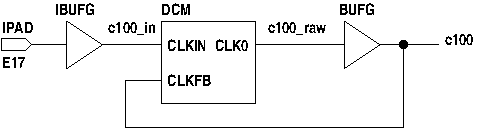
\includegraphics{dcm}
            
            To generate a divided clock as well -
            \begin{lstlisting}[gobble=12, language=threepl]
               iopins(c100_pin, "E17");
               float(c100_freq, 100.0e6);
               float(clock_ratio, 2.0);
               clock(c100_in, frequency=c100_freq, loc=c100_pin, ibufg=true);
               clock({global.c100, c100_raw}, frequency=c100_freq);
               clock({global.c50, c50_raw}, frequency=c100_freq/clock_ratio);
               attributes(c100, tnm="C100");
               attributes(c50, tnm="C50");
               clkdcm(
                   clk0=c100_raw,
                   clkdv=c50_raw
                   <-
                   clkin=c100_in,
                   clkfb=c100,
                   clkdv_divide=tostring(clock_ratio)
               );
               clockbufg(c100 <- c100_raw);
               clockbufg(c50 <- c50_raw);
            \end{lstlisting}
            
            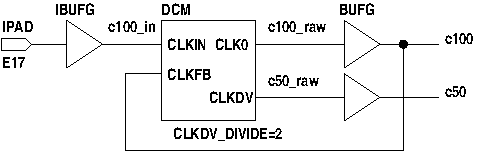
\includegraphics{dcm2}
            
            Note that in the above example the tnm attributes have been
            assigned using inbuilt procedure attributes() rather than as
            an argument to clock().

            In a CPLD the input clock can be used directly as a clock domain.

%============== THIS SECTION NEEDS TO BE CHECKED ==============================
        \subsection{DDR input}

            \index{DDR}
            For double data rate input two flip-flops are used in each IOB, one
            clocked directly and the other clocked via an inverter. The output
            of the -ve edge flip-flop must then be clocked on the next +ve edge
            into another flip-flop so that both bits are available in one clock
            domain.
            
            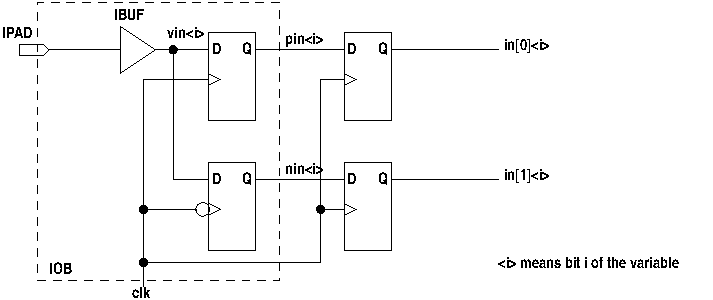
\includegraphics{ddrin}
            
            At present the Xilinx place-and-route tools accept the following
            code, but a more direct approach will be implemented shortly.

            \begin{lstlisting}[gobble=12, language=threepl]
               iopins(pins, "[]str", {"A1", "A2", "A3", "A4"});
               negclock(nclk, clk);
               input(vin, "bits:4", loc=pins);
               static(pin, "bits:4"); attributes(pin, continuous=true);
               static(nin, "bits:4"); attributes(nin, continuous=true);
               static(in, "[2]bits:4"); attributes(in, continuous=true);

               useclock(clk);
               pin <- vin;

               useclock(nclk);
               nin <- accept(vin);

               useclock(); // back to previous clock domain, clk
               in[0] <- pin;
               in[1] <- accept(nin);
            \end{lstlisting}
            When a negative clock is created using inbuilt procedure
            {\bf negclock()} the positive clock is still used but it is
            flagged such that an inverter is inserted at every logic element
            which uses it. Clock inverters are built in to all Xilinx
            clocked elements.
            
            Note the use of accept() to allow the assignment despite the different
            clock domains. It is not clear if the Xilinx place-and-route tools will
            generate and apply a half-period constraint between flip-flops clocked
            on opposite clock edges. These paths contain no logic, only routing,
            and hence tight timing constraints can be expected to be easily met.

        \subsection{DDR output}

            \index{DDR}
            For double data rate input two flip-flops are used in each IOB, one
            clocked directly and the other clocked via an inverter. The outputs
            of the two flip-flops are multiplexed to the output buffer and pad
            (using the positive clock I assume). The data must be clocked from
            two preceding flip-flops clocked with the positive clock.
            
            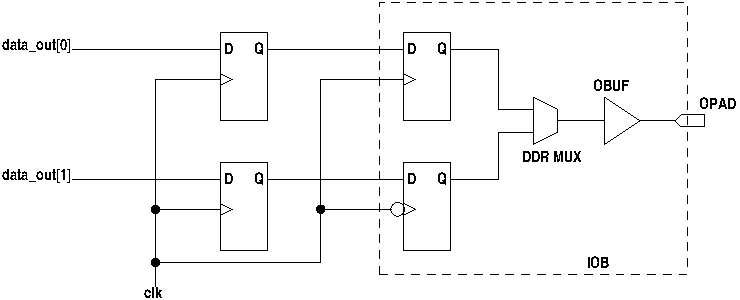
\includegraphics{ddrout}
            
            At present DDR output is not implemented, but will be shortly.


%=============================================================================



    \section{Floating point}
    
        \index{type!floating point}
        Immediate floating point values are stored in 64 bit IEEE 754 single
        precision form with a biased exponent of 8 bits and a mantissa of 23
        bits. The usual arithmetic can be used with these to form expressions.
             
        Target floating point values are stored as a struct with fields for the
        sign, biased exponent and mantissa. Thus target floating point types
        are not actually primitive.
        
        Apart from the creation of floating point variables target floating
        point is not explicitly supported by 3PL. Since target floating types
        are represented by associated structs they can be assigned to
        variables and passed as arguments to parameters. Since they are handled
        as structs the following limitations apply -
        \blist
        \item   Target floating point variables cannot be
                used in expressions. This restriction is imposed because the
                complexity of floating point operations dictates that pipelining
                should be used to achieve a reasonable throughput. Since
                operators in expressions must be capable of executing in one
                cycle if the operands are available, internal pipelining cannot
                be used by expression operators. If target floating point
                operators were implemented (which is easy enough to do) a very
                low clock frequency would have to be used to allow time for
                complete operations to be executed. The alternative adopted is
                to use library modules to carry out target floating point
                operations, these being pipelined to sustain a high throughput
                at the cost of latency.
        \item   Assignment of target floating point values cannot perform
                size adjustment and hence the left and right sides must match
                exactly in type. Where floating point sizes are to be changed
                library functions exist to do this.
        \item   Floating point parameters in modules, procedures or
                functions must either match their arguments exactly in type
                or else must have their type omitted, in which case they will
                be given the type of the argument.
        \item   Where immediate floating point arguments are passed to
                target floating point parameters the immediate values are
                converted to target floating point values with constant fields.
                These are structs of equivalent type "float:23.8". The
                parameters must either be exactly this type or else must have
                the type omitted.
        \blend
        
        For target floating point arithmetic operations there is a library,
        {\bf float.3pl} (see \autorefph{chap:fp}), which contains modules
        implementing pipelined add, subtract, multiply and divide.







    \section{Unbuffered queues}\label{sec:unbufferedqueues}
     
        \index{queue!unbuffered}
        \index{unbuffered queues}
        An unbuffered queue is one whose depth has been set to zero (by 'depth=0'
        as an attribute passed to inbuilt procedure queue() or using the {\bf
        attributes()} \autorefph{sec:ipattributes} inbuilt procedure to set it
        afterwards). For queue creation see {\bf queue()}
        \autorefph{sec:ipqueue}. These are used to synchronise two execution
        threads, optionally passing a datum in the process. A thread writing to
        an unbuffered queue will wait until a read is executed on that queue and
        vice versa. The situation is symmetrical with respect to the reader and
        writer, each waiting on the other. The read and write will execute on the
        same clock cycle.
        
        Unbuffered queues can only be synchronous, not asynchronous.
        
        Unbuffered queues cannot be initialised.
        
        An unbuffered queue may be of type "null" if no data is to be transmitted.

        An unbuffered queue cannot be read or written within -
        \blist
        \item   a {\bf waitpri} statement.
        \item   a {\bf waitprilock} statement.
        \item   a {\bf sync} statement.
        \item   a {\bf sync when} statement.
        \blend
        
        An unbuffered queue can be read or written within other control
        structures.
        
        An unbuffered queue can not be an argument to the \verb'?:' ternary
        conditional operator.
        
        A waitprilock can be used to avoid simultaneous writes to an unbuffered
        queue as long as an unbuffered queue access is not contained within
        the subject statement of the waitprilock, for example -
        
        \begin{lstlisting}[gobble=8, language=threepl]
           queue(ubq, "uint:8", depth=0);
           static(v, "uint:8");
           priority(p);

           seq {
               .
               .
               waitprilock(p, 1)
                    ;   // null subject statement
               ubq <<- 3;
               priunlock(1);
               .
           }
        \end{lstlisting}
        
        The above restrictions are required because an unbuffered queue uses
        signalling between reader and writer which is not compatible with the
        signalling used for buffered queues. When a read or write to an
        unbuffered queue is initiated that raises the available flag for the
        complementary write or read. When the complementary write or read occurs
        the opposite availability flag is briefly raised and then the read and
        write transaction is completed. If both the read and the write to an
        unbuffered queue were waiting on queue availability before proceeding then
        deadlock would occur since availability requires the initiation of the
        other side of the transaction. The second read or write operation of a
        transaction pair could employ normal synchronisation with other queues,
        but to allow this would provide too many opportunities for deadlock and
        hence the above restrictions have been imposed and enforced.
        
        An unbuffered queue can have its read or write availability tested using
        the \verb'>' or \verb'<' unary operators. Read availability will be true
        when a write is pending. In the case of a chain of assignments containing
        unbuffered queues read availability will be true when all upstream
        assignments are ready to execute and have read availability themselves.
        When an unbuffered queue has read availability its value can be examined
        using the (\verb'?' unary operator). Write availability will be true when
        a read is pending. In the case of a chain of assignments containing
        unbuffered queues write availability will be true when all downstream
        assignments are ready to execute and have write availability themselves.
        
        An assignment statement may have an unbuffered queue on the LHS and
        multiple buffered and unbuffered queues on the right hand side. The
        assignment will wait for the RHS buffered queues to be available and the
        RHS unbuffered queues to have a write pending. Reads from multiple
        unbuffered queues in an expression will wait until all unbuffered queues
        have writes able to proceed.

        An unbuffered queue may be read in more than one place and may be written
        in more than one place. In the case of multiple writers they must be
        mutually exclusive. waitprilock() statements may be used to ensure this.
        Any pending reads of an unbuffered queue will wait until a write to that
        queue after which they will continue along their execution threads.
        Unlike buffered queues the modules in which unbuffered queue reads are
        situated are not significant, i.e. unbuffered queues behave as though the
        'ignore\_modules' attribute was set (the 'ignore\_modules' attribute
        itself is ignored).

        In general unbuffered queues may be passed to modules, procedures and
        functions. Unbuffered queues cannot however be passed to inbuilt
        procedures which produce inline target code such as cmemorywrite(),
        rmemoryread() and rmemorywrite().

        Unbuffered queues are intended for synchronisation of execution threads
        usually, but not necessarily, within loops. Such loops may be implicit
        as with top level {\bf seq} or {\bf par} blocks or may be explicit
        (target {\bf while} or target {\bf do while}). The following illustrates
        a simple case -
        
        \begin{lstlisting}[gobble=8, language=threepl]
           queue(ubq, "uint:8", depth=0);
           static(v, "uint:8");

           seq {
               .
               .
               ubq <<- 3;
               .
               .
           }

           seq {
               .
               .
               v <- ubq;
               .
               .
           }
        \end{lstlisting}
        
        The first sequential thread to reach the queue access will wait for
        the other. After the write and read take place simultaneously the
        two threads will continue sequential execution and then repeat.
        
        The master-slave concept described earlier can be used to implement
        an initiation and acknowledgment scheme. A master write can be issued
        to initiate some process. The slave process waits using the read
        availablility operator. When this returns true the slave can examine
        the data using the examine operator and then execute the controlled
        operation. Meanwhile the write will hang waiting for availability.
        When the slave side has finished it can then execute a read to release
        the master write. If data is to be transfered in the other direction
        on acknowledgement then the master would be a read and the slave a
        write. An example of the former is given below -
        
        \begin{lstlisting}[gobble=8, language=threepl]
           queue(ubq, "uint:8", depth=0);

           // master thread
           static(status, type(ubq));
           seq {
               ubq <- ...;      // initiate the slave process
               .                // continue the thread
               .
               .
           }

           // slave thread
           when (<ubq) seq {
               branch (?ubq) {  // perform operations based on the examined value
               case .....
               .
               .
           }
           null <<- ubq;        // do a read to release the write in the master thread
        \end{lstlisting}
        
        By checking read availability the slave thread detects the write by the
        master thread. It then examines the written value rather than reading it,
        thus leaving the master write suspended. Finally the slave thread
        releases the master thread by doing a read. Since the data value is not
        now needed it can be dumped into null.
        
        Note that this mechanism is valid for chains of unbuffered queue
        assignments and applies to any point along that chain.
        
        Where an acknowledge status is to be returned the master reads and
        the slave writes -
        \begin{lstlisting}[gobble=8, language=threepl]
           queue(ubq, "uint:8", depth=0);

           // master thread
           static(status, type(ubq));
           seq {
               status <- ubq;   // initiate the slave process waiting for return
               .                // do something with the returned status
               .
               .
           }

           // slave thread
           when (>ubq) {
               .                // perform operations
               .
               .
               ubq <<- ...;     // return a status
           }
        \end{lstlisting}
        The master thread will initiate a read, but the queue is unavailable
        as there is no matching write from the slave. The slave however
        sees that there is write availability as a result of the master read.
        It goes ahead with thread execution and on completion writes a
        status value. The write-read transaction now completes and the master
        thread continues.

        An assigment may have multiple buffered and unbuffered queues on its
        RHS, for example -
        \begin{lstlisting}[gobble=8, language=threepl]
            type(t, "uint:8");
            queue({ubq1, ubq2}, t, depth=0);
            queue({q1, q2}, t);
            static(v, t);
           
            seq {
                .
                q1 <<- ...;
                .
            }
           
            seq {
                .
                q2 <<- ...;
                .
            }
           
            seq {
                .
                ubq1 <<- ...;
                .
            }
           
            seq {
                .
                ubq2 <<- ...;
                .
            }

            seq {
            .
                v <- q1 + ubq1 + q2 + ubq2;
                .
            }
        \end{lstlisting}
        
        The assignments to buffered queues q1 and q2 will occur when
        encountered (if these queues are not full). The assigment at the
        bottom will wait until q1 and q2 are not empty and writes are pending
        on ubq1 and ubq2. The writes to ubq1 and ubq2 will also wait until
        the last assignment statement is able to execute. When that happens
        that last seq block will move on as will the two seq blocks containing
        the writes to ubq1 and ubq2.




\pagebreak

\chapter{Inbuilt Modules}

    \index{module!inbuilt}
    The following called modules are built into the compiler. User
    called modules or procedures must not use identifiers that conflict
    with these.
    
    The following abbreviations are used to denote modes -

    \begin{tabular}{| l | l |}
    \hline
    I  & immediate      \\ \hline
    IN & input          \\ \hline
    V  & value          \\ \hline
    SV & selectvalue    \\ \hline
    S  & static         \\ \hline
    Q  & queue          \\ \hline
    M  & memory         \\ \hline
    PR & priority       \\ \hline
    C  & clock          \\ \hline
    \end{tabular}
    
    The following abbreviations are used to denote types -

    \begin{tabular}{| l | l |}
    \hline
    bits & bits                                                 \\ \hline
    uint & unsigned integer                                     \\ \hline
    int & integer or unsigned integer                           \\ \hline
    fixed & fixed point                                         \\ \hline
    float & floating point                                      \\ \hline
    log & logical (boolean)                                     \\ \hline
    str & string                                                \\ \hline
    type & type                                                 \\ \hline
    any & any type                                              \\ \hline
    prim & a primitive type                                     \\ \hline
    comp & a compound type (arrays, structs or any combination) \\ \hline
    [] & array of type                                          \\ \hline
    \end{tabular}


    Modules with 'yes' to 'Parameter=argument allowed' can have arguments
    matched to parameters by position in the argument list or by
    parameter=argument (keymatch) or a mixture as long as positional arguments
    do not follow keymatch arguments. Otherwise these keymatch arguments are
    not allowed. This may be because - \\
    \blist
    \item   the module has a single input or output argument in which case
    no positional or keymatch parameter association is needed
    \item   the module has an indefinite number of arguments and hence there
    are no 'named' parameters with which to associate arguments
    \blend
    The keymatching may be restricted to just input or just output.


    \section{del - variable length delay line}\label{sec:imdel}
        
        {\bf Call:} \\
        del(out \verb'<-' in, len, init, step, varlen, reset);
        
        {\bf Output parameters:} \\
        \begin{tabular}{| l | l | l | l |}
        \hline
        param  & mode & type  & \\
        \hline \hline
        out  & V & any & output \\ \hline
        \end{tabular}
        
        {\bf Input parameters:} \\
        \begin{tabular}{| l | l | l | l |}
        \hline
        param  & mode & type  & \\
        \hline \hline
        in     & V & any  & input          \\ \hline
        len    & I & int  & optional line fixed delay \\ \hline
        init   & I & any  & optional initialisation \\ \hline
        step   & V & log  & optional line step \\ \hline
        varlen & V & uint & optional line variable delay \\ \hline
        reset  & V & log  & optional line reset \\ \hline
        \end{tabular}
        
        {\bf Parameter=argument allowed:} \\
        Input arguments only.
        
        {\bf Description:} \\
        This module is a delay line implemented using CLB shift registers or
        flip-flops. On each clock cycle the input is written to the line and the
        contents move one item right. The rightmost item appears as the out
        value. This module can function as a sequence generator if the output
        is connected back to the input.
        
        This module is used extensively internally by 3PL to generate single
        cycle delays in execution threads in which context it is implemented as
        a single flip-flop.
        
        For large delays this uses a lot of CLBs and the alternative library
        function {\bf delay()} \autorefph{sec:lfdelay} in library stdlib.3pl
        might be preferable. That library function will call {\bf del()}
        in any case if the delay value is small enough.

        This has 1 to 6 input arguments and 1 output argument. Input arguments
        {\bf len} and {\bf init} are immediate mode. {\bf step} may be
        immediate or target mode as described below. The other input arguments
        must not be modes {\bf immediate}, {\bf queue}, {\bf memory} or {\bf
        clock} and value mode arguments must not contain queue reads.
        
        None of the arguments to this module can contain queue reads. This
        limitation could be easily removed but it is felt that the resulting
        behaviour of this module could become unduly complex. In limited
        circumtances this limitation can be worked around and there are examples
        below to illustrate this.

        The 1st input argument, {\bf in}, is the delay line data input. It can
        be any target type.

        The optional input argument, {\bf len}, specifies a fixed delay.
        This must be an immediate int. If this argument is 0 or omitted and the
        5th argument {\bf varlen} is also omitted, the output will simply be
        connected to the input to give zero delay.

        The optional input argument, {\bf init}, is an initialisation array.
        This  must be immediate mode and an array of the same type as {\bf in}.
        It may be smaller than the delay line length in which case the input end
        of the delay line will be zero initialised. The low order entries in
        the initialisation array are loaded in the output end of the delay line.
        Thus for example a delay of 5 initialised to \{1, 2, 3\} will output
        1 2 3 0 0.
        If initialisation values are too large their high-order bits will be
        truncated.

        The optional input argument, {\bf step}, is a line step enable.
        This  must be type log. If this argument is used the line will only
        advance when {\bf step} is true, otherwise the line will advance on
        every clock cycle.

        The optional input argument, {\bf varlen}, is a variable line
        length. This must be type uint. This argument may be limited or
        unavailable depending on the type of FPGA. For Xilinx the variable
        length is limited to values between 0 and 15 giving delays of 1 to 16
        respectively. A wider argument will be truncated and a narrower one
        zero padded. Note that when the line length is changed data may be
        skipped or repeated. If the line length is changed while stepping is
        inhibited, the line length argument is an address with which the
        contents of the line can be non-destructively examined.

        The optiona input argument, {\bf reset}, returns the
        line to its initial state when true.

        The output argument, {\bf out}, is the delay line data output. This
        argument must be value mode and must be the same type as the data
        input {\bf in}.
        
        If the delay line is initialised, these initial values appear at the
        output during the initial {\em n} line steps, where {\em n} is the
        fixed delay (or the initial delay selected by {\bf varlen}
        if used).
        
        For Xilinx the following apply -
        \blist
        \item   For FPGAs prior to Virtex5 the variable length argument is limited to values
                between 0 and 15 inclusive, giving line lengths of 1 to
                16 respectively. From Virtex5 onwards the lengths are 1 to 32.
        \item   If the reset is used, the variable length argument cannot be
                used.
        \item   If the reset is used or the variable length parameter is not
                used and the delay is 3 or less, the delay line will be
                implemented using flip-flops, otherwise it will be implemented
                using CLB LUT shift registers.
        \blend
        Implementation using CLB LUT shift registers minimises resources,
        requiring only one CLB LUT for every 16-bit delay line.
        
        {\bf Note: the fixed delay parameter {\em len} gives the number of cycles
        to be delayed but the variable delay parameter {\em varlen} is the
        number of cycles delay minus one!}      
            
        In Xilinx devices there is a substantial delay between the clock edge
        and the arrival of the shift register signal at the output of the logic
        block (2.8nS to 3.5nS for a -6 speed XC2VP and about 1.15 to 1.43nS
        for  a -2 speed XC5V). The delay for a flip-flop is very much smaller.
        For this reason a delay line with fixed length is implemented using a
        flip-flop for the last delay stage. If a variable length delay line is
        required, this flip-flop is not inserted and hence the significant
        output delay must be considered. It is preferable in that case to
        assign the delay line output directly to a variable, i.e. with no
        intervening combinatorial logic, to avoid introducing any extra path
        delay.
        
        The limitation stated above that inputs cannot contain queue reads
        can be overcome in some cases. For example to use a queue as data input
        we can use the examine operator as long as a queue wait controls the
        delay step. For example to form a running average of length 8 -

        \begin{lstlisting}[gobble=12, language=threepl]
            queue(q, "uint:8");
            static(rsum, "uint:11");
            queue(rav, "uint:8");
            value(out, "uint:8");
            
            del(out <- ?q, 8,, <q);     // there is no queue read here!
            
            seq {
                rsum <- rsum + q - out; // there is a queue read here
                rav <<- rsum / 8;
            }
        \end{lstlisting}
        Here a data stream is written to queue {\bf q} and a running average
        appears as a stream through queue {\bf rav}. The data input does not
        contain a queue read as the examine operator simply looks at the queue
        output, valid or not, and does not pop a datum. It is important to note
        that the read availability of {\bf q} is tested in two places, the
        reading of {\bf q} and the expression {\bf \verb'<q'}. Although {\bf
        del()} is a distinct module {\bf \verb'<q'} is evaluated as an argument
        to {\bf del()} in the current scope, not the scope of {\bf del()}, so
        there is only a single destination to {\bf q}, or rather both
        availability tests are in the same destination module.
        
        Another approach is used in library function {\bf del()} in
        xilinx/common.3pl \autorefph{sec:lfdel} which calls inbuilt module
        {\bf del()}.
        


       


    \section{resync - resynchronise a level}\label{sec:imresync}
        
        {\bf Call:} \\
        resync(out \verb'<-' in);
        
        {\bf Output parameters:} \\
        \begin{tabular}{| l | l | l | l |}
        \hline
        param & mode & type & \\
        \hline \hline
        out & V & log & output pulse \\ \hline
        \end{tabular}
        
        {\bf Input parameters:} \\
        \begin{tabular}{| l | l | l | l |}
        \hline
        param & mode & type & \\
        \hline \hline
        in    & V SV S PR & log & target value pulse or level \\ \hline
        \end{tabular}
        
        {\bf Parameter=argument allowed:} \\
        No
        
        {\bf Description:} \\
        {\bf in} is an expression or a value, selectvalue, static, input or
        priority variable of type log.
        
        {\bf out} is a value of type log.

        When the input rises and is sampled by the clock associated
        with that variable, the output will produce a single cycle pulse
        synchronised with the current clock domain.

        If the input is an input, selectvalue, static or priority mode variable
        and it has not yet been referenced or assigned then it will be
        given the current clock domain. An unassigned value variable
        will also be given the current clock domain. A value variable that
        has been assigned but has a null clock domain will result in error
        termination.



\pagebreak

\chapter{Inbuilt Procedures}

    \index{procedure!inbuilt}
    The following procedures are built into the compiler. User
    called modules or procedures must not use identifiers that conflict
    with these.
    
    The following abbreviations are used to denote modes -

    \begin{tabular}{| l | l |}
    \hline
    I  & immediate                      \\ \hline
    V  & value                          \\ \hline
    SV & selectvalue                    \\ \hline
    S  & static                         \\ \hline
    Q  & queue                          \\ \hline
    CM & combinatorial output memory    \\ \hline
    RM & registered output memory       \\ \hline
    PR & priority                       \\ \hline
    IN & input                          \\ \hline
    O  & output                         \\ \hline
    C  & clock                          \\ \hline
    \end{tabular}
    
    The following abbreviations are used to denote types -

    \begin{tabular}{| l | l |}
    \hline
    bits  & bits                                                    \\ \hline
    uint  & unsigned integer                                        \\ \hline
    int   & integer or unsigned integer                             \\ \hline
    fixed & fixed point                                             \\ \hline
    float & floating point                                          \\ \hline
    log   & logical (boolean)                                       \\ \hline
    str   & string                                                  \\ \hline
    enum  & enumerated type                                         \\ \hline
    type  & type                                                    \\ \hline
    file  & file                                                    \\ \hline
    map   & map                                                     \\ \hline
    list  & list                                                    \\ \hline
    any   & any type                                                \\ \hline
    prim  & a primitive type                                        \\ \hline
    comp  & a compound type (arrays, structs or any combination)    \\ \hline
    []    & array of type                                           \\ \hline
    \end{tabular}

    Procedures with 'yes' to 'Parameter=argument allowed' can have arguments
    matched to parameters by position in the argument list or by
    parameter=argument (keymatch) or a mixture as long as positional arguments
    do not follow keymatch arguments. The keymatch arguments may be in
    any order. Otherwise these keymatch arguments are
    not allowed. This may be because - \\
    \blist
    \item   the procedure has a single input or output argument in which case
    no positional or keymatch parameter association is needed
    \item   the procedure has an indefinite number of arguments and hence there
    are no 'named' parameters with which to associate arguments
    \blend
    The keymatching may be restricted to just input or just output.

    Procedures with 'yes' to in-line target execution will produce in-line
    code in the FPGA. This code is controlled by the execution stream in which
    it is embedded and by the availability of any queues in the arguments.
    Other procedures do not produce in-line code in the FPGA. However, they may 
    produce target components which are accessed by in-line target code
    elsewhere in the source code.
        


    \section{addmodeattribute - add attribute to the mode attribute map}\label{sec:ipaddmodeatt}
        
        {\bf Call:} \\
        addmodeattribute(mode, key, isarray, type);
        
        {\bf Output parameters:} \\
        none
        
        {\bf Input parameters:} \\
        \begin{tabular}{| l | l | l | l |}
        \hline
        param  & mode & type & \\
        \hline \hline
        mode    & I & str & mode           \\ \hline
        key     & I & str & attribute      \\ \hline
        isarray & I & log & is an array    \\ \hline
        type    & I & str & primitive type \\ \hline
        \end{tabular}
        
        {\bf Parameter=argument allowed:} \\
        Yes
        
        {\bf In-line target execution:} \\
        No
        
        {\bf Description:} \\
        Add an attribute to the attribute map for a variable mode. 3PL contains
        an internal map initialised with entries for allowed attributes for each
        mode. These attributes are internal to 3PL and affect the netlist
        generation. Attributes from which constraints are generated are not
        handled internally by 3PL but by library code appropriate to the FPGA
        platform. To allow centralised vetting of attributes in calls to inbuilt
        procedures input(), output() and clock() this procedure is used to add
        these constraint attributes to the map.
        
        {\bf mode} is a string identifying the mode and is "input", "output"
        or "clock"
        
        {\bf key} is the attribute name.
        
        {\bf isarray} is true if the attrbute value is an array (one member
        for each bit). If not an array the value will be duplicated for
        each bit.
        
        {\bf type} is the attribute value primitive type and can be "uint",
        "float", "log" or "str" as appropriate.



        
    \section{append - append a list entry}\label{sec:ipappend}
        
        {\bf Call:} \\
        append(list, index, value);
        
        {\bf Output parameters:} \\
        none
        
        {\bf Input parameters:} \\
        \begin{tabular}{| l | l | l | l |}
        \hline
        param  & mode & type & \\
        \hline \hline
        list   & I     & list & a list   \\ \hline
        index  & I     & int  & an index   \\ \hline
        value  & I V C & any  & the value   \\ \hline
        \end{tabular}
        
        {\bf Parameter=argument allowed:} \\
        Yes
        
        {\bf In-line target execution:} \\
        No
        
        {\bf Description:} \\
        The item {\bf value} is appended at the position indicated by {\bf
        index} in list {\bf list}. The index may range from 0 to {\bf
        entries(list)} inclusive. If {\bf index} is outside this range a fatal
        error occurs. An index of 0 inserts at the beginning of the list and
        an index equal to the list size appends to the end of the list. If
        the index argument is omitted the item will be appended to the end
        of the list. If the last argument is omitted null will be appended.
        
        The appended item may be immediate, clock, cmemory or rmemory mode.


    \section{appendall - append entries from another list}\label{sec:ipappendall}
        
        {\bf Call:} \\
        appendall(l, l2);
        
        {\bf Output parameters:} \\
        none
        
        {\bf Input parameters:} \\
        \begin{tabular}{| l | l | l | l |}
        \hline
        param  & mode & type & \\
        \hline \hline
        l      & I     & list & a list   \\ \hline
        l2     & I     & list & another list   \\ \hline
        \end{tabular}
        
        {\bf Parameter=argument allowed:} \\
        No
        
        {\bf In-line target execution:} \\
        No
        
        {\bf Description:} \\
        The contents of list {\bf l2} are appended at the position indicated
        by {\bf index} in list {\bf l}. The index may range from 0 to {\bf
        entries(l)} inclusive. If {\bf index} is outside this range a fatal
        error occurs. An index of 0 inserts at the beginning of the list and
        an index equal to the list size appends to the end of the list. If
        the index argument is omitted the items will be appended to the end
        of the list.
        


    \section{argadjust - adjust arguments for arithmetic operations}\label{sec:ipargadjust}
        
        {\bf Call:} \\
        argadjust(out1, out2, rt \verb'<-' in1, in2, op, matchleft);
        
        {\bf Output parameters:} \\
        \begin{tabular}{| l | l | l | l |}
        \hline
        param  & mode     & type & \\
        \hline \hline
        out1   & V        & -    & adjusted first operand   \\ \hline
        out2   & V        & -    & adjusted second operand  \\ \hline
        rt     & I        & type & result type              \\ \hline
        \end{tabular}
        
        {\bf Input parameters:} \\
        \begin{tabular}{| l | l | l | l |}
        \hline
        param      & mode & type & \\
        \hline \hline
        in1        & V    & -    & first operand   \\ \hline
        in2        & V    & -    & second operand  \\ \hline
        op         & I    & str  & operation       \\ \hline
        matchleft  & I    & log  & use left offset \\ \hline
        \end{tabular}
        
        {\bf Parameter=argument allowed:} \\
        Yes
        
        {\bf In-line target execution:} \\
        No
        
        {\bf Description:} \\
        This procedure takes two value mode arguments and an operator and
        supplies two adjusted values and a result type. The input operands
        (the 1st and 2nd arguments) must be type "uint:", "int:", "ufixed:"
        or "fixed:". The 3rd input argument, the operator type, must be
        one of the strings "+", "*" or "/".
        
        This procedure accesses code within the 3PL interpreter used for
        adjusting target variables in arithmetic expressions.
        
        The "+" operator is used for addition and "-" for subtraction but the
        action is identical. The operand with the smaller offset will be
        adjusted to match the other, i.e. the binary points will be aligned
        by left shifting the operand with fewer fractional bits. The type
        assigned to the 3rd output argument will have the same binary point
        offset as the now-adjusted operands and the integer part will be
        one bit wider than the operand with the largest integer part.
        
        If the 4th input argument is supplied and is true, the result offset
        will be the same as the first input operand and the second input operand
        will be adjusted by left or right shifting as required. This feature
        is included for the case where the first operand is the result of
        an intermediate hardware operation and is not accessible for adjustment
        (for example in an XC5V DSP block where a multiplication can be followed
        by an addition or subtraction but the intermediate product cannot be
        adjusted).
        
        The "*" operator is used for multiplication. The operands are not
        adjusted and are returned as the output values. The output result type
        fraction width is the sum of the operand fraction widths and the
        integer width is the sum of the operand integer widths.
        
        The "/" operator is used for division. The operands are not
        adjusted and are returned as the output values. The output result type
        fraction width is the sum of the numerator fraction width and the
        denominator integer width. The result integer width is the sum of the
        numerator integer width and the denominator fraction width.



    \section{assert - assert a value mode variable for a clock cycle}\label{sec:ipassert}
        
        
        {\bf Call:} \\
        assert(v \verb'<-' o);
        
        {\bf Output parameters:} \\
        \begin{tabular}{| l | l | l | l |}
        \hline
        param & mode & type & \\
        \hline \hline
        v & V & log & value carrying the pulse \\ \hline
        \end{tabular}
        
        {\bf Input parameters:} \\
        \begin{tabular}{| l | l | l | l |}
        \hline
        param & mode & type & \\
        \hline \hline
        or & I & log & if true, OR with previous value \\ \hline
        \end{tabular}
        
        {\bf Parameter=argument allowed:} \\
        No
        
        {\bf In-line target execution:} \\
        yes
        
        {\bf Description:} \\
        This procedure asserts a logical value variable true for one clock cycle
        when this statement executes. The value is true for the clock cycle
        leading up to the clock edge on which execution occurs.

        If the input argument is provided and is true the output value variable
        will be assigned the OR of its previous value and the execution pulse.
        If it has no previous assigned value it is assigned the execution pulse.
        Using this optional input argument a signal pulsed from more than one
        place can be generated. {\bf Note: when ORed in this way, use of the
        value of the output variable must follow the last call to assert() since
        each call re-assigns the value mode variable!}

        If the ORing option is not selected and multiple calls to
        {\bf assert()} are made with the same output argument, each call will
        re-assign the output value variable, which may be what is wanted or
        may not!
        
        The following code illustrates some points to consider -
        \begin{lstlisting}[gobble=8, language=threepl]
           value({l, v1, v2}, "log");
           static(v, "log");

           when (l) seq {
               ....
               .
               .
               par {
                   assert(v1 <-);
                   v2 <- true;
               }
               v2 <- false;
               .
           }
        \end{lstlisting}
        
        'v1' and 'v2' will both be be true for one clock cycle, but 'v1' will
        be asserted one clock cycle earlier than 'v2'. Use of {\bf assert()}
        has the potential disadvantage that since it is actually the execution
        signal it suffers any delays inherent in the logic path of any
        conditional and hence might introduce timing constraint difficulties.
        
        Note that the following usage is allowed -
        \begin{lstlisting}[gobble=8, language=threepl]
           value(v, "log");

           when (v) 
               ....
           .
           .
           assert(v <-);
           .
        \end{lstlisting}
        Here the call to {\bf assert()} occurs only once. 3PL notices when
        assigning a value to {\bf v} within the call to {\bf assert()} that
        {\bf v} has been referenced previously at which time it had not
        been assigned a value, so it takes care of the post-assignment
        (see discussion of post-assignment in section \ref{sec:im_valass}).
        The following {\bf would not work in the same way} -
        \begin{lstlisting}[gobble=8, language=threepl]
           value(v, "log");

           when (v)
               ....
           .
           .
           assert(v <-);
           .
           assert(v <- true);   // PROBABLY WRONG!
           .
        \end{lstlisting}
        The second call to {\bf assert()} would indeed OR the two execution
        signals together and assign the result to variable {\bf v}, but the
        {\bf when ()} would use the value of {\bf v} after the first call
        to {\bf assert()}. Since with parallel code the order of statements
        is not significant, it would clearly be better to use a policy of
        referencing the variable following all calls to {\bf assert()}.

        see also inbuilt function {\bf used()} \autorefph{sec:ifused}.


    \section{attributeprocedure - register a procedure to handle attributes}\label{sec:ipattributeproc}
        
        {\bf Call:} \\
        attributeprocedure(p);
        
        {\bf Output parameters:} \\
        none
        
        {\bf Input parameters:} \\
        \begin{tabular}{| l | l | l | l |}
        \hline
        param & mode & type  & \\
        \hline \hline
        p     & - &  -  & procedure identifier \\ \hline
        \end{tabular}
        
        {\bf In-line target execution:} \\
        No
        
        {\bf Description:} \\
        This procedure registers the argument procedure as a user-defined procedure
        to handle input, output and clock mode attributes. The registered procedure
        will be called after every input, output and clock mode variable is
        created. The called procedure will be passed a single argument which is a
        pointer to the newly-created variable.

        This facility is intended to allow attributes to be attached to I/O pin
        specifications and have them transferred to relevant input, output or
        clock mode variables when those variables are created. It can also provide
        any necessary re-formatting of attributes, either those brought in from pin
        associations or those passed as arguments to inbuilt procedures input(),
        output() or clock().
        
        There is a Xilinx library procedure for this purpose;
        {\bf processPinAttributes()} \autorefph{sec:lpprocPinAtt},
        in xilinx/common.3pl.
        
        attributeprocedure() should be called prior to calls to inbuilt procedures
        input(), output() or clock().
        



    \section{attributes - assign attributes to a variable}\label{sec:ipattributes}
        
        {\bf Call:} \\
        attributes(v, attr);
        
        {\bf Output parameters:} \\
        none
        
        {\bf Input parameters:} \\
        \begin{tabular}{| l | l | l | l |}
        \hline
        param & mode & type  & \\
        \hline \hline
        v     & any &  -  & variable identifier \\ \hline
        attr  & I   & map & attributes map      \\ \hline
        \end{tabular}
        
        {\bf Parameter=argument allowed:} \\
        No
        
        {\bf In-line target execution:} \\
        No
        
        {\bf Description:} \\
        This procedure applies attributes to one or more variables. The first
        argument may be a compound value containing a number of identifiers for
        created variables. Identifiers may have fields or subscripts appended
        but these will be ignored, the attribute(s) being applied to the
        entire variable.
        
        The optional second argument can be
        \blist
        \item   a map of attributes
        \item   a one-dimensional compound constant containing key=value entries
        \item   a key=value argument
        \blend
        
        In the last case this may be followed by more key=value arguments. If this
        is not supplied the attributes can be added later using inbuilt procedure
        {\bf attributes()} \autorefph{sec:ipattributes}. For a description of
        applicable attributes see \autorefph{sec:attributes}.
        
        Attributes are applied to a variable in a map. The map
        keys are the attribute identifiers and the associated values
        are the attribute values. The entry values are mixed types,
        the type depending on the individual attribute.

        A compound value can be used for the attributes argument. It
        must be a one-dimensional list and every entry must be
        key=value format.

        The attributes() procedure does not enter a new attributes map in
        the variable, it adds the entries in the argument map to that in the
        variable. Thus the attributes() procedure can be called multiple times
        to add one or more attributes to the variable. If the same attribute is
        entered again the new value replaces the old value. This can be used to
        enable and disable 3PL attributes that are used during immediate
        execution.

        Netlist attributes can be deleted by assigning the value {\bf null}.
        3PL attributes cannot be deleted; 3PL attributes either
        relate to parameters that are mandatory such as clock domains, or are
        boolean in which case they can be disabled rather than deleted, so
        there is no reason to delete them.
        
        3PL attributes {\bf domain}, {\bf readdomain} and {\bf writedomain} may be
        assigned null which is interpreted to mean that the current clock domain is
        to be used.
        
        {\bf Note that for input, output and clock mode variables many of the
        attributes are ignored by 3PL itself and must be processed by 3PL source
        code. These modes are handled by inbuilt procedures input(), output() and
        clock() which call a library procedure named by
        attributeprocedure()\autorefph{sec:ipattributeproc} to process the
        attributes. These attributes will also be added to the variable but 3PL
        itself will ignore them.}
        
        Attributes are described in the sections pertaining to the relevant
        variable creation procedures.



    \section{change - change a list entry}\label{sec:ipchange}
        
        {\bf Call:} \\
        change(list, index, value);
        
        {\bf Output parameters:} \\
        none
        
        {\bf Input parameters:} \\
        \begin{tabular}{| l | l | l | l |}
        \hline
        param  & mode & type & \\
        \hline \hline
        list   & I     & list & a list   \\ \hline
        index  & I     & int  & an index   \\ \hline
        value  & I V C & any  & the value   \\ \hline
        \end{tabular}
        
        {\bf Parameter=argument allowed:} \\
        Yes
        
        {\bf In-line target execution:} \\
        No
        
        {\bf Description:} \\
        The item in list {\bf list} at position {\bf index} is replaced by item
        {\bf value}. The index may range from 0 to {\bf entries(l) - 1}
        inclusive. If {\bf index} is outside this range a fatal error
        occurs. The new value does not have to be the same type as the
        previous value. If the last argument is omitted the list item will
        be changed to null.
        
        The new item may be immediate, clock, cmemory or rmemory mode.


    \section{class - create a variable of type "class"}\label{sec:ipclass}

        {\bf Call:} \\
        class(c, init);

        {\bf Output parameters:} \\
        None.

        {\bf Input parameters:} \\            
        {\bf init} is an immediate value of type "class".
        
        {\bf Parameter=argument allowed:} \\
        No

        {\bf In-line target execution:} \\
        no

        {\bf description:} \\
        This procedure creates one or more variables of type "class".
        
        The first argument is the variable identifier, or it can be a
        comma-separated list of identifiers enclosed in braces.
        
        The second argument is optional and is an initial value for the variable.
        It is only allowed where a single variable is being created. The "class"
        value may be from another variable of the same type but more usually it
        would be the returned value from a call to a class, for example the
        following creates a variable {\bf cl} of type "class" and assigns to it
        an instance of the class {\bf c} returned from a call to {\bf c()}.

        \begin{lstlisting}[gobble=8, language=threepl]
            class(cl, c());
            .
            .
            
            class c () {
                .
                .
                .
            }
        \end{lstlisting}



    \section{clock - create one or more clock variables}\label{sec:ipclock}
        
        {\bf Call:} \\
        clock(ident, ....);
        
        {\bf Output parameters:} \\
        none
        
        {\bf Input parameters:} \\
        \begin{tabular}{| l | l | l | l |}
        \hline
        param  & mode & type  & \\
        \hline \hline
        ident or \verb'{'id1, id2... \verb'}' & - &  -  & variable identifier(s)   \\ \hline
        .... & - & - & optional attributes \\ \hline
        \end{tabular}
        
        {\bf Parameter=argument allowed:} \\
        No
        
        {\bf In-line target execution:} \\
        No
        
        {\bf Description:} \\
        Create a clock variable.

        Create one or more clock mode variables.
        
        {\bf ident} is the variable identifier. If more than one
        variable is to be created the list of variables must be in braces
        {\em \{id1, id2, \dots\}}. The variable identifier can also be constructed
        from a string by using the indirect operator on a string variable or
        parenthesised expression, see subsection \autorefph{subsec:strvarcreat}.
        
        When a {\bf loc} attribute is provided only a single clock variable
        can be created by this procedure.
        
        When {\bf clock()} is used to create a module, procedure or function
        parameter it cannot be passed attributes. The created parameter variable
        will adopt the attributes of the associated argument.
        
        Any following arguments specify attributes. Each argument may specify an
        attribute by keymatch format, i.e. attribute=value where 'attribute' is
        an attribute identifier and 'value' is an appropriate mode and type.
        Alternatively an argument can be a map containing attributes where the
        key (string) is the attribute identifier and the associated value is
        the attribute value.

        Attributes may also be associated with the input pin or pin pair. This is
        described in chapter \autorefph{chap:cpa} {\bf Constraints, Properties and
        Attributes} where other aspects of processing attributes and constraints
        for input, output and clock mode variables are also described.

        Attributes can be added by using inbuilt procedure {\bf attributes()}
        \autorefph{sec:ipattributes}.             
        
        Attributes are required for two main purposes; control of netlist
        generation and constraint file entries. Attributes giving input pin
        locations and input buffer types directly control netlist generation.
        I/O standards and timing group names exercise control of place-and-route
        via a constraint file.
              
        The applicable attributes are shown in the following table.

                These attributes are not case-sensitive but will be converted to
        lower case.
         
        The attribute values will be applied to all pins.
        
        \btabularx
        \hline
        \multicolumn{4}{|l|}{\bf clock mode} \\
        \hline
        frequency    & 3PL     & float         & frequency, Hz \\
        dutycycle    & 3PL     & float         & duty cycle    \\
        differential & netlist & log           & differential  \\
        ibufg        & netlist & log           & buffer type   \\
        loc          & netlist & str or [2]str & locations     \\
        \hline
        \btabularxend
        
        Attributes {\bf frequency} and {\bf dutycycle} specify these parameters
        for clock nets and any associated clock domains. {\bf Note that at
        present dutycycle is not used. It has been included for future use.}

        The following attribute is read-only and is created when inbuilt
        procedure {\bf clock()} is called and can be retrieved from the clock
        mode variable if required by the function call attribute("ids").
        
        \btabularx
        \hline
        \multicolumn{3}{|l|}{\bf clock mode} \\
        \hline
        ids          & 3PL & []str & element IDs       \\
        \hline
        \btabularxend
        
        The following attributes only apply to a clock variable if it is a clock
        input from a pad. If the {\bf loc} attribute is supplied to a clock
        variable an input pad and buffer will be created, otherwise the clock
        variable source is internal to the FPGA.

        {\bf loc} specifies one or two pad locations (FPGA pins) for the clock
        input - two locations if it is differential (+ve, -ve order). For a
        differential clock input this attribute will be an array of two strings.

        {\bf differential} indicates that the clock input is differential - two
        locations must be supplied and the buffer will be an IBUFDS or IBUFGDS
        rather than the default IBUF or IBUFG. This attribute is used internally
        by 3PL for code generation.

        {\bf ibufg} if true specifies that the input buffer must be an IBUFG or
        IBUFGDS instead of the default IBUF or an IBUFDS. This attribute is used
        internally by 3PL for code generation. It is not clear from Xilinx
        documentation that an IBUFG needs to be explicitly specified, or if
        instead this can be inferred from the package pin(s). other software. 

        The following attributes are required for constraint generation and are
        handled at completion of immediate execution by library procedure {\bf
        generateconstraints()} \autorefph{sec:lpgenerateconstraints}. The
        attribute values are single values which will be applied to the pin or
        pins.
        
        \btabularx
        \hline
        \multicolumn{4}{|l|}{\bf clock mode constraint attributes} \\
        \hline
        tnm          & constraint & str & timing group id                       \\
        diff\_term   & constraint & log & differential  $100\Omega$ termination \\
        iostandard   & constraint & str & voltage standard                      \\
        \hline
        \btabularxend

        {\bf tnm} is the name of a timing group in which all state devices
        clocked by this clock are to be included for timing constraint purposes.
        All clocks which drive logic clock inputs (as distinct from inputs to
        buffers of clock managers) will have a period constraint generated by
        generate\_constraints() in xilinx/common.3pl. By default a timing group
        name will be constructed from the clock identifier translated to upper
        case, but if a "tnm" attribute is provided then this string will be used
        instead.        

        {\bf diff\_term} indicates that a $100\Omega$ termination resistance should
        be applied to a differential input.

        {\bf iostandard} is a string specifying one of the allowed I/O standards
        (see Xilinx documentation).

        The following attribute is read-only and is added when target statement
        variables are assigned or evaluated and the clock domain is established
        or verified. It can be retrieved from the clock mode variable if
        required by the function call attribute("valid").
        
        \btabularx
        \hline
        \multicolumn{3}{|l|}{\bf clock mode} \\
        \hline
        valid   & 3PL & log & is a valid logic clock    \\
        \hline
        \btabularxend

        Any attributes that are not listed above will result in a fatal error.

                
        Where the call to {\bf clock()} is to create a parameter to a module,
        procedure or function, only the first argument may be given and it must be
        a single identifier. The clock frequency, period and duty cycle are
        copied from the matching argument.
        
        Where a clock variable is an external input the {\bf loc} attribute
        must be supplied. This would be an array of two location strings for
        a differential clock input or a singlr location string otherwise.

        As far as the compiler is concerned any clock variable may be used to
        control logic (by calling inbuilt procedure {\bf useclock()}). However,
        many clock variables are used as routing to connect clock managers,
        input pads, buffers etc together and these interconnect clock variables
        must not be passed to {\bf useclock()}.
       
        Note: for each pin a netlist port "PORT\_pin" is created where 'pin' is
        the pin identifying string. This port name is also the netlist identifier
        of the netlist from the output of the pad to the input of the IBUFG.
        This convention can be used when generating associated constraints.



    \section{clockfromexpr - drive a clock from an expression}\label{sec:ipclockfromexpr}

        {\bf Call:} \\
        clockfromexpr(clk \verb'<-' expr);

        {\bf Output parameters:} \\
        {\bf clk} is a clock variable.

        {\bf Input parameters:} \\            
        {\bf expr} is an expression of type log which is to drive the clock.
        
        {\bf Parameter=argument allowed:} \\
        No

        {\bf In-line target execution:} \\
        no

        {\bf description:} \\
        This procedure connects a clock signal to an expression. That
        clock signal would normally then be buffered using a global clock
        buffer created by library procedure {\bf clockbufg}.
        The argument may be input, selectvalue, value, static or priority mode
        but must be type log and must contain no queue references.



    \section{close - close a file}\label{sec:ipclose}
        
        {\bf Call:} \\
        close(file);
        
        {\bf Output parameters:} \\
        none
        
        {\bf Input parameters:} \\
        \begin{tabular}{| l | l | l | l |}
        \hline
        param  & mode & type  & \\
        \hline \hline
        file & I & file & file variable   \\ \hline
        \end{tabular}
        
        {\bf Parameter=argument allowed:} \\
        No
        
        {\bf In-line target execution:} \\
        No
        
        {\bf Description:} \\
        This procedure closes an open file.



%    \section{connect - connect two signals}\label{sec:ipconnect}
%        
%        {\bf Call:} \\
%        connect(vsink \verb'<-' vsrc);
%        
%        {\bf Output parameters:} \\
%        \begin{tabular}{| l | l | l | l |}
%        \hline
%        param  & mode & type  & \\
%        \hline \hline
%        vsink & V & log & value variable   \\ \hline
%        \end{tabular}
%        
%        {\bf Input parameters:} \\
%        \begin{tabular}{| l | l | l | l |}
%        \hline
%        param  & mode & type  & \\
%        \hline \hline
%        vsrc & V & log & value variable   \\ \hline
%        \end{tabular}
%        
%        {\bf Parameter=argument allowed:} \\
%        No
%        
%        {\bf In-line target execution:} \\
%        No
%        
%        {\bf Description:} \\
%        This procedure connects two signals. The two arguments must be value
%        mode.
%        
%        {\bf This is intended solely for use where basic library elements are being
%        used so that, for example, location constraints can be applied.
%        \index{location constraint}
%        \index{constraint!location}
%        It is not intended for use in normal high-level 3PL code.} This procedure
%        is needed where the outputs of basic library elements are to be connected
%        on 3-state nets, e.g. BUFT, BUFE, PULLUP, PULLDOWN, KEEPER.


    \section{cmemory - create a combinatorial output memory}\label{sec:ipcmemory}
        \index{variable!memory!combinatorial output}
        
        {\bf Call:} \\
        cmemory(id, ports, atype, dtype, init, ...);
        
        {\bf Output parameters:} \\
        none
        
        {\bf Input parameters:} \\
        \begin{tabular}{| l | l | l | l |}
        \hline
        param  & mode       & type  & \\
        \hline \hline
        id     & -  &  -    & memory identifier         \\ \hline
        ports  & I  & int   & number of ports           \\ \hline
        atype  & I  & int   & address type              \\ \hline
        dtype  & I  & int   & data type                 \\ \hline
        init   & I  & []int & optional initialisation (variable or compound
                              constant)                 \\ \hline
        ...    & I  &  -    & optional attributes       \\ \hline
        \end{tabular}
        
        {\bf Parameter=argument allowed:} \\
        Yes
        
        {\bf In-line target execution:} \\
        No
        
        {\bf Description:} \\
        Procedure {\bf cmemory()} creates a combinatorial output RAM.        
        {\bf cmemory()} may create a module, procedure or function
        parameter in which case only the first argument is needed (the memory
        identifier).

        In the case of Xilinx FPGAs combinatorial output memory is
        distributed CLB RAM. This can have one or two access ports. One
        logic slice can hold 1 bit x 32 words single port or 1 bit x 16
        words dual port.

        Port 0 can be read or written (or both). Port 1 is read-only.
        
        {\em id} is an identifier for the memory. The variable identifier can
        also be constructed from a string by using the indirect operator on a
        string variable or parenthesised expression, see subsection
        \autorefph{subsec:strvarcreat}.

        {\em ports} is the number of ports. This argument may be by position or
        by ports=x where x is a constant or immediate variable. For Xilinx FPGAs
        theis must be 1 or 2.

        {\em atype} is the address type. This can be any target type but
        would normally be type "uint:". The type has the constraint that the total number of
        bits must not exceed 9. This argument may be by position or by
        atype=x where x is a string specifying a type or else a type variable.       

        {\em dtype} is the data type. This can be any target type. This argument
        may be by position or by dtype=x where x is a string specifying a type
        or else a type variable.
        
        {\em init} is an optional initialisation array. The initialisation data
        is a one-dimensional variable or array which is no larger than the depth
        of the memory. It may be smaller in which case the memory is zero
        padded. The types and structure of the initialisation variable or
        structured constant after the first dimension must match the memory data
        type. Immediate constants are padded to fit target elements but must not
        exceed the target width. If the initialisation argument is omitted the
        memory will be initialised to all zero. This argument may be by position
        or by init=x where x is an immediate array variable. For compound types
        the immediate type must match the target data type but omitting the data
        widths. The target type can be converted to a matching immediate type
        by the builtin function {\em targtoimtype()}.
        
        Where the {\em init} argument is supplied in the call to cmemory() the
        argument may be compound constant, though this is not usually practical as
        {\em init} is usually a large array. Otherwise the argument will be
        an immediate variable of appropriate type. The initialising variable must be a
        matching type to the target data type of the memory. The initial value
        variable can be created from the target data type by calling builtin function
        {\bf targtoimtype()} \autorefph{sec:iftargtoimtype} -

        \begin{lstlisting}[gobble=8, language=threepl]
            struct (st,
                f1, "uint:30",
                f2, "uint:30"
            );
            var(init, "[8]" + targtoimtype(st));
            init[0].f1 = ....;
            init[0].f2 = ....;
            .
            .
            .
            var(init0, targtoimtype(st));
            init0.f1 = ..;
            init0.f2 = ..;
            cmemory(m, 1, atype="uint:3", dtype=st, init=init);
        \end{lstlisting}
            
        {\em init} can be assigned to a memory
        variable, along with attributes, later in execution by calling
        builtin procedure {\bf attributes()}\autorefph{sec:ipattributes}, e.g.
        \begin{lstlisting}[gobble=8, language=threepl]
            cmemory(m, 1, atype="uint:3", dtype=st);
            attributes(m, init=init);
        \end{lstlisting}
        but in this case the argument must be an immediate variable, not a compound
        constant. The call to attributes() can be any time after calling
        cmemory() and (obviously) before termination of execution.

        There may be trailing arguments following the optional {\em init} which supply
        memory attrbutes, described in a table below. {\em init} is included amongst
        the attributes for convenience. These arguments must all be of the form
        attribute=value. These may be included in the call to cmemory() or else passed
        later using builtin procedure attributes().

                \btabularx
        \hline
        \multicolumn{4}{|l|}{\bf cmemory mode attributes} \\
        \hline
        init       & 3PL       &                      & initial value                    \\
        domain     & 3PL       & clock                & force clock domain for all ports \\     
        \hline
        \btabularxend
        
        {\bf These attributes are case-insensitive.}
        
        {\bf init} sets an initial value for the memory. Any previous initial
        value will be overwritten. The initial value must be a compound type and
        the nested type must be an immediate type equivalent to the memory data
        type, i.e. same type but without a width field. The initial value is not
        used until completion of immediate execution when variables are
        processed into target code and hence it can be changed at any time
        during immediate execution.

        {\bf domain} forces the clock domain (both input and output) for all
        ports to the specified clock domain. If assigned {\bf null} the current
        clock domain is selected. If the variable already has a clock domain as
        a result of having been assigned or evaluated then that clock domain is
        compared with the intended domain. If the assigned clock domain agrees
        with that already in place then there is no further action, otherwise a
        fatal error occurs.


        Architectures supported -

        \begin{tabular}{| l | l |} \hline
        Spartan-II, Spartan IIE         & YES   \\ \hline
        Spartan-3                       & YES   \\ \hline
        Virtex, Virtex-E                & YES   \\ \hline
        Virtex-II, Virtex-II Pro        & YES   \\ \hline
        XC9500, XC9500XV, XC9500XL      & NO    \\ \hline
        Coolrunner XPLA3, Coolrunner-II & NO    \\ \hline
        \end{tabular}

        The range of memory depths that have been implemented is shown in the
        following table. The depth required is determined from the number of bits
        in the address type. Memories with depths smaller than the minimum listed
        are still implemented, but the physical memory will be the minimum size
        shown and the smaller depth will be achieved by tying higher address bits
        low. The column marked ROM is for memories that are initialised and are
        read but not written -

        \begin{tabular}{| l | l | l | l |} \hline
                                & ROM       & 1 port   &   2 port   \\ \hline \hline
        Spartan-II, Spartan IIE & 16 -  256 & 16 -  256 & 16 -  128 \\ \hline
        Spartan-3               & 16 - 2048 & 16 -  512 & 16 -  128 \\ \hline
        Virtex                  & 16 -  256 & 16 -  256 & 16 -  256 \\ \hline
        Virtex-E                & 16 -  256 & 16 -  256 & 16 -  256 \\ \hline
        Virtex-II               & 16 - 2048 & 16 - 1024 & 16 -  512 \\ \hline
        Virtex-II Pro           & 16 - 2048 & 16 - 1024 & 16 -  512 \\ \hline
        Virtex 4                & 16 - 2048 & 16 -  512 & 16 -  128 \\ \hline
        Virtex 5                & 16 - 4096 & 16 - 4096 & 16 - 2048 \\ \hline                                             
        \end{tabular}

        The data may be any width.
        
        Applicable attributes are shown in the following table. The
        attributes can be passed as arguments to this procedure or may be
        applied to the variable using the inbuilt procedure
        {\bf attributes()} \autorefph{sec:ipattributes}.
        
        When {\bf cmemory()} is used to create a module, procedure or function
        parameter it cannot be passed attributes. The created parameter variable
        will adopt the attributes of the associated argument.



    \section{cmemorywrite - write to a combinatorial output memory}\label{sec:ipcmemorywrite}
        
        {\bf Call:} \\
        cmemorywrite(id, port, addr, data);
        
        {\bf Output parameters:} \\
        none
        
        {\bf Input parameters:} \\
        \begin{tabular}{| l | l | l | l |}
        \hline
        param  & mode     & type  & \\
        \hline \hline
        id   & M             &  -  & memory being written   \\ \hline
        port & I             & int & port                   \\ \hline
        addr & I V SV S Q PR & any & memory address         \\ \hline
        data & I V SV S Q PR & any & data to be written     \\ \hline
        \end{tabular}
        
        {\bf Parameter=argument allowed:} \\
        Yes
        
        {\bf In-line target execution:} \\
        yes
        
        {\bf Description:} \\
        Write to a port of a combinatorial output memory.

        {\em id} is the memory mode variable identifier.

        {\em port} is the memory port.

        {\em addr} is the address.

        {\em data} is the data to be written.
        
        The data and address may be any type, including compound types, but the
        types must match the types given when the combinatorial output memory was
        created (see {\bf cmemory()} \autorefph{sec:ipcmemory}) but primitive
        component widths may differ in which case padding or truncation will occur.

        Xilinx FPGAs do not allow writes to port 1. Within this limitation
        multiple reads and writes on a port are allowed and the address and
        data inputs will be multiplexed, however there is no access arbitration
        and it is up to the application code to ensure exclusive access.
        Coincident accesses will result in data corruption.

        A call to {\bf cmemorywrite()} (\autorefph{sec:ipcmemorywrite}) or {\bf
        cmemoryread()} (\autorefph{sec:ifcmemoryread}) sets the clock domain for
        the memory port to the current clock domain. All further calls to either of
        these inbuilt procedures for the same port of the same combinatorial output
        memory must be in the same clock domain (or a fatal error results).


    \section{designname - change the design name}\label{sec:ipdesignname}
        
        {\bf Call:} \\
        designname(name);
        
        {\bf Output parameters:} \\
        none
        
        {\bf Input parameters:} \\
        \begin{tabular}{| l | l | l | l |}
        \hline
        param  & mode & type & \\
        \hline \hline
        name   & I    & str  & design name string   \\ \hline
        \end{tabular}
        
        {\bf Parameter=argument allowed:} \\
        No
        
        {\bf In-line target execution:} \\
        no
        
        {\bf Description:} \\
        Change the design name, overriding the default derived from
        the file name. This can be overridden by the command line option
        {\bf -N}. It is also overridden if inbuilt procedure {\bf export()}
        is called.



    \section{directive - enter a directive}\label{sec:ipdirective}
        
        {\bf Call:} \\
        directive(key, value);
        
        {\bf Output parameters:} \\
        none
        
        {\bf Parameter=argument allowed:} \\
        No
        
        {\bf Input parameters:} \\
        \begin{tabular}{| l | l | l | l |}
        \hline
        param  & mode     & type  & \\
        \hline \hline
        key   & I & str & directive key                 \\ \hline
        value & I & any & directive value (optional)    \\ \hline
        \end{tabular}
        
        {\bf In-line target execution:} \\
        No
        
        {\bf Description:} \\
        There is a single global directive map. The key is a string.  The value
        may one of the 3PL immediate primitive types {\bf int}, {\bf log}, {\bf
        float} or {\bf str}. If the second argument is not provided the entry
        will be type {\bf log} and value {\bf true}.
        
        If the directive is already present its value will be changed but
        the type must be the same or a fatal error will occur.
               
        see also inbuilt procedures \\
        {\bf presetdirective()} \autorefph{sec:ippresetdirective} \\
        {\bf removedirective} \autorefph{sec:ipremovedirective}. \\
        and inbuilt functions \\
        {\bf directive()} \autorefph{sec:ifdirective}.\\
        {\bf direxists()} \autorefph{sec:ifdirexists}.\\
        {\bf directives()} \autorefph{sec:ifdirectives}.



    \section{divrem - combined quotient and remainder}\label{sec:ipdivrem}

        {\bf Prototype:} \\
        \vsp
        \begin{lstlisting}[gobble=8, language=threepl]
           procedure
           divrem (quot, rem <- num, denom) {}
        \end{lstlisting}
        
        {\bf Output parameters:} \\
        \begin{tabular}{| l | l | l | l |}
        \hline
        param  & mode     & type  & \\
        \hline \hline
        quot   & V & int uint & quotient    \\ \hline
        rem    & V & int uint & remainder   \\ \hline
        \end{tabular}
        
        {\bf Input parameters:} \\
        \begin{tabular}{| l | l | l | l |}
        \hline
        param  & mode     & type  & \\
        \hline \hline
        num    & I & int uint & numerator   \\ \hline
        denom  & I & int uint & denominator \\ \hline
        \end{tabular}
        
        {\bf Parameter=argument allowed:} \\
        Yes

        {\bf In-line target execution:} \\
        no

        {\bf description:} \\
        This procedure takes numerator and denominator values and
        computes the quotient and remainder. The results appear on
        output value variables since this procedure is combinatorial.
        The input and output types must be all{\em int} or all {\em uint}
        (widths may be different). The inputs may be immediate.

        {\nf Note: this procedure uses cascaded adders and subtractors
        and may have a very long data path delay!} However, the code is
        optimised for some cases where one operand is constant -  for
        division of 0 (return 0:0), division by 1 (return n:0) and
        division by power of 2 (quotient by shifting, remainder by
        masking).




    \section{element - add an element to the EDIF netlist}\label{sec:ipelement}
        
        {\bf Call:} \\
        element(name, id);
        
        {\bf Output parameters:} \\
        none
        
        {\bf Input parameters:} \\
        \begin{tabular}{| l | l | l | l |}
        \hline
        param  & mode     & type  & \\
        \hline \hline
        name & I & str & element name                     \\ \hline
        id   & I & str & optional unique block identifier \\ \hline
        \end{tabular}
        
        {\bf Parameter=argument allowed:} \\
        No
        
        {\bf In-line target execution:} \\
        No
        
        {\bf Description:} \\
        This procedure adds an element to the EDIF netlist. This is intended for
        special elements, perhaps particular to a specific FPGA family. For
        example global clock buffers are not considered generic enough to be
        included as fundamental logic elements so they are included using this
        procedure. A family-specific example would be the high-speed serial
        interfaces. Note that this is a low level process that bypasses 3PL
        execution streams. It is rather similar to embedding assembly code within
        a high level language.
        
        The first argument is the Xilinx library element name, e.g.
        {\bf element("BUFG")}.
        
        The second argument is an optional unique block identifier. If this
        argument is omitted then an identifier of the form "e123" will be alloted.
        {\bf Explicit identifiers must avoid the forms "e123" and "b123" to avoid
        conflicts with 3PL internally generated element identifiers.}
        
        Regardless of explicit use of the block identifer or not, the element
        constructed by this procedure remains as the current element until
        another call to this procedure. Connections to the element are made by
        the inbuilt procedures {\bf elementinput()}, {\bf elementclockinput()},
        {\bf elementoutput()} or {\bf elementtsoutput()} (see links below). The
        construction of an element must be completed by calling inbuilt
        procedure {\bf elementend()} \autorefph{sec:ipelementend}. Properties
        for the element are added by calling inbuilt procedure {\bf
        elementproperty()} \autorefph{sec:ipelementproperty}. Associated entries
        to the NCF file for the element can be made using inbuilt
        procedure {\bf elementaddncf()} \autorefph{sec:lpelementaddncf}.
        
        Note that this procedure can also be used to add standard elements to
        the netlist, e.g. {\bf element(, "FDRE")}.
        
        Elements defined by using {\bf element()} are added to cell definitions in
        the EDIF file. If another element of the same cell name is created they
        will share the same cell definition. The ports in the cell definition will
        be the set of all input, output or three-state ports specified in all
        instances of the element. Thus an instance of an element may not specify
        all the available ports for the element but the cell definition will
        accumulate all ports specified in the instances of the element. Any
        available ports not specified will be omitted from the cell definition.
        In the case of array ports where the port width
        changes from instance to instance the largest dimension will be used in
        the cell definition.
        
        For further description see \autorefph{chap:asfpgahe}.

        See also - \\
        {\bf elementend()} \autorefph{sec:ipelementend}, \\
        {\bf elementproperty()} \autorefph{sec:ipelementproperty}, \\
        {\bf elementinput()} \autorefph{sec:ipelmntin}, \\
        {\bf elementclockinput()} \autorefph{sec:ipelmntinclk} \\
        {\bf elementoutput()} \autorefph{sec:ipelmntout} \\
        {\bf elementtsoutput()} \autorefph{sec:ipelmntoutts}.




    \section{elementclockinput - connect a clock input signal to an EDIF netlist element}\label{sec:ipelmntinclk}
        
        {\bf Call:} \\
        elementclockinput(id, port\_name, signal);
        
        {\bf Output parameters:} \\
        none
        
        {\bf Input parameters:} \\
        \begin{tabular}{| l | l | l | l |}
        \hline
        param  & mode     & type  & \\
        \hline \hline
        id          & I          & str & optional block identifier \\ \hline
        signal      & V SV S Q I & any & optional signal           \\ \hline
        port\_name  & I          & str & port name                 \\ \hline
        \end{tabular}
        
        {\bf Parameter=argument allowed:} \\
        Yes
        
        {\bf In-line target execution:} \\
        No
        
        {\bf Description:} \\
        This procedure connects a clock input signal to an element (see {\bf
        element()} \autorefph{sec:ipelement}).

        The block identifier {\bf id} specifies the element to which a port is
        to be added. If this argument is omitted then the most recent element
        begun by a call to {\bf element} is assumed.

        Creation of multiple elements may be interleaved, but it is preferable
        to avoid interleaving and to complete an element before starting the
        next.

        {\bf port\_name} is a string identifying the element port to be
        connected.

        {\bf signal} is the signal to be connected to the element port. It must
        be clock mode or else an immediate type "log" whose value is false, in
        which case the clock input will be connected to GND. This argument may
        also be an immediate mode string in which case it refers to a single
        FPGA port (PAD), the string value being the pin designation. For a
        string "AB12" the port name will be "PORT\_AB12". The element port must
        be a single bit.

        If the {\bf signal} argument is missing or null the port will be
        connected to ground.

        This procedure should only be used for clock inputs to elements where
        the input functions as an edge trigger. Thus for inputs to clock buffers
        or the source inputs to clock managers {\bf elementinput()}
        \autorefph{sec:ipelmntin} should be used instead. This distinction was
        once required so that 3PL could keep track of clock destinations for
        timing constraint generation, however this is no longer the case. A
        remnant remains in the {\bf clk\_sinks} and {\bf clk\_CE} read-only
        attributes of clock mode variables.

        See also - \\
        {\bf element()} \autorefph{sec:ipelement}, \\
        {\bf elementend()} \autorefph{sec:ipelementend}, \\
        {\bf elementproperty()} \autorefph{sec:ipelementproperty}, \\
        {\bf elementinput()} \autorefph{sec:ipelmntin}, \\
        {\bf elementoutput()} \autorefph{sec:ipelmntout}, \\
        {\bf elementtsoutput()} \autorefph{sec:ipelmntoutts}.




    \section{elementend - complete construction of an EDIF netlist element}\label{sec:ipelementend}
        
        {\bf Call:} \\
        elementend(id);
        
        {\bf Output parameters:} \\
        none
        
        {\bf Input parameters:} \\
        \begin{tabular}{| l | l | l | l |}
        \hline
        param  & mode     & type  & \\
        \hline \hline
        id         & I    & str & optional block identifier \\ \hline
        \end{tabular}
        
        {\bf Parameter=argument allowed:} \\
        No
        
        {\bf In-line target execution:} \\
        No
        
        {\bf Description:} \\
        This procedure is called to complete entry of a netlist element.
        The optional argument gives the block identifier of the element
        to be completed. If omitted, the most recent uncompleted element
        is assumed.



    \section{elementinput - connect an input signal to an EDIF netlist element}\label{sec:ipelmntin}
        
        {\bf Call:} \\
        elementinput(id, port\_name, signal, arrayformat);
        
        {\bf Output parameters:} \\
        none
        
        {\bf Input parameters:} \\
        \begin{tabular}{| l | l | l | l |}
        \hline
        param  & mode     & type  & \\
        \hline \hline
        id          & I          & str & optional block identifier \\ \hline
        port\_name  & I          & str & port name                 \\ \hline
        signal      & V SV S Q I & any & signal                    \\ \hline
        arrayformat & I          & int & array format indicator    \\ \hline
        \end{tabular}
        
        {\bf Parameter=argument allowed:} \\
        Yes
        
        {\bf In-line target execution:} \\
        No
        
        {\bf Description:} \\
        This procedure connects an input signal to an element (see {\bf element()}
        \autorefph{sec:ipelement}).
        
        The block identifier {\bf id} specifies the element to which a port is to
        be added. If this argument is omitted then the most recent
        element begun by a call to {\bf element} is assumed.
        
        Creation of multiple elements may be interleaved, but it is preferable to
        avoid interleaving and to complete an element before starting the next.
        
        {\bf port\_name} is a string identifying the element port to be
        connected. The port width is determined by the signal width.

        
        {\bf signal} is the signal to be connected to the element port. It may be
        value, selectvalue, or static and may be any type. If value mode the value
        must not contain any queue reads. This argument may also be an immediate mode
        string in which case it refers to a single FPGA port (PAD), the string value
        being the pin designation. For a string "AB12" the port name will be
        "PORT\_AB12". If the signal is more than one bit wide an array format
        argument must be provided.

        If the {\bf signal} argument is missing or null no port connection is
        made.
               
        {\bf arrayformat} indicates the form of ports which are arrays.
        If this argument is 1 it indicates that array ports should be
        expanded to individual pins of the form A0, A1, A2 etc. If the value
        is 2 then the port will be a formal EDIF array. ISE will accept format
        1 for all elements. Some versions of ISE (e.g. 10) give errors when
        format 2 is used for block RAM elements where different port sizes
        are used in the same configuration. Vivado requires format 2 for port
        arrays. Since Vivado cannot be used for earlier FPGAs, block RAMs for
        these (up to XCS6, XCV6) are defined using format 1. Series 7 block RAMs
        are defined using format 2 since early versions of ISE do not support
        these devices. A single bit port can have a format type of 1, but not
        type 2.
        
        In the case of clock mode inputs this procedure should only be used for
        inputs to elements where the input does not function as an edge trigger, e.g.
        for inputs to clock buffers or the source inputs to clock managers. For edge
        trigger inputs {\bf elementclockinput()} \autorefph{sec:ipelmntinclk} should
        be used instead. This distinction was once required so that 3PL could keep
        track of clock destinations for timing constraint generation, however this
        is no longer the case. A remnant remains in the {\bf clk\_sinks} and
        {\bf clk\_CE} read-only attributes of clock mode variables.

        As an example of port input, the code -
        
        \begin{lstlisting}[gobble=8, language=threepl]
           input(is, "log", loc="AB12", tnm="IC");
        \end{lstlisting}
        
        could be effectively replaced by -
        
        \begin{lstlisting}[gobble=8, language=threepl]
           value(is, "log");

           ibuf(is <- "AB12", "IC");

           module
           ibuf (value(out) <- str(pin), str(tnm)) {
               element("IBUF");
               elementinput(, "I", pin);
               elementoutput(out <- , "O");
               elementStrProperty(, "loc", pin);
               elementend();
               IOconstraint(pin, "tnm", "IC");
           }
        \end{lstlisting}
        
        though note that the variable {\bf is} would now be value mode, not
        input mode.

        See also - \\
        {\bf element()} \autorefph{sec:ipelement}, \\
        {\bf elementend()} \autorefph{sec:ipelementend}, \\
        {\bf elementproperty()} \autorefph{sec:ipelementproperty}, \\
        {\bf elementclockinput()} \autorefph{sec:ipelmntinclk} \\
        {\bf elementoutput()} \autorefph{sec:ipelmntout}, \\
        {\bf elementtsoutput()} \autorefph{sec:ipelmntoutts}.





    \section{elementoutput - connect an output signal to an EDIF netlist element}\label{sec:ipelmntout}
        
        {\bf Call:} \\
        elementoutput(signal \verb'<-' id, port\_name, arrayformat);
        
        {\bf Output parameters:} \\
        \begin{tabular}{| l | l | l | l |}
        \hline
        param  & mode     & type  & \\
        \hline \hline
        signal      & V SV S Q I & any & signal                    \\ \hline
        \end{tabular}
        
        {\bf Input parameters:} \\
        \begin{tabular}{| l | l | l | l |}
        \hline
        param  & mode     & type  & \\
        \hline \hline
        id          & I          & str & optional block identifier \\ \hline
        port\_name  & I          & str & port name                 \\ \hline
        arrayformat & I          & int & array format indicator    \\ \hline
        \end{tabular}
        
        {\bf Parameter=argument allowed:} \\
        Yes
        
        {\bf In-line target execution:} \\
        No
        
        {\bf Description:} \\
        This procedure connects an output signal to an element (see {\bf element()}
        \autorefph{sec:ipelement}).
        
        The block identifier {\bf id} specifies the element to which a port is to
        be added. If this argument is omitted then the most recent
        element begun by a call to {\bf element} is assumed.
        
        Creation of multiple elements may be interleaved, but it is preferable to
        avoid interleaving and to complete an element before starting the next.
        
        {\bf signal} is the signal to be connected to the element port. It must be
        value mode, of any type, or clock mode. This argument may also be an
        immediate mode string in which case it refers to a single FPGA port (PAD),
        the string value being the pin designation. For a string "AB12" the port
        name will be "PORT\_AB12" (see input example in {\bf elementinput()}
        \autorefph{sec:ipelmntin}). If the signal is more than one bit wide an
        array format argument must be provided.        
        
        {\bf port\_name} is a string identifying the element port to be
        connected. The port width is determined by the signal width.
        
        {\bf arrayformat} indicates the form of ports which are arrays.
        If this argument is 1 it indicates that array ports should be
        expanded to individual pins of the form A0, A1, A2 etc. If the value
        is 2 then the port will be a formal EDIF array. ISE will accept format
        1 for all elements. Some versions of ISE (e.g. 10) give errors when
        format 2 is used for block RAM elements where different port sizes
        are used in the same configuration. Vivado requires format 2 for port
        arrays. Since Vivado cannot be used for earlier FPGAs, block RAMs for
        these (up to XCS6, XCV6) are defined using format 1. Series 7 block RAMs
        are defined using format 2 since early versions of ISE do not support
        these devices. A single bit port can have a format type of 1, but not
        type 2.

        See also - \\
        {\bf element()} \autorefph{sec:ipelement}, \\
        {\bf elementend()} \autorefph{sec:ipelementend}, \\
        {\bf elementproperty()} \autorefph{sec:ipelementproperty}, \\
        {\bf elementinput()} \autorefph{sec:ipelmntin}, \\
        {\bf elementclockinput()} \autorefph{sec:ipelmntinclk} \\
        {\bf elementtsoutput()} \autorefph{sec:ipelmntoutts}.






    \section{elementproperty - set an element property}\label{sec:ipelementproperty}
        
        {\bf Call:} \\
        elementproperty(id, property, value);
        
        {\bf Output parameters:} \\
        none
        
        {\bf Input parameters:} \\
        \begin{tabular}{| l | l | l | l |}
        \hline
        param  & mode     & type  & \\
        \hline \hline
        id       & I        & str & optional block identifier \\ \hline
        property & I        & str & property name             \\ \hline
        value    & I        & str & property value            \\ \hline
        \end{tabular}
        
        {\bf Parameter=argument allowed:} \\
        Yes
        
        {\bf In-line target execution:} \\
        No
        
        {\bf Description:} \\
        This procedure sets a property value for an element.
        The optional argument {\bf id} gives the block identifier of the element
        to be completed. If omitted, the most recent uncompleted element
        is assumed.

        {\bf elementproperty()} only takes strings as value arguments so a number
        of library procedures are available in xilinx/common.3pl to format other
        types. These are - \\
        {\bf elementLogProperty()} \autorefph{sec:lpelementLogProperty}, \\
        {\bf elementIntProperty()} \autorefph{sec:lpelementIntProperty}, \\
        {\bf elementBinProperty()} \autorefph{sec:lpelementBinProperty}, \\
        {\bf elementHexProperty()} \autorefph{sec:lpelementHexProperty}, \\
        {\bf elementFloatProperty()} \autorefph{sec:lpelementFloatProperty}, \\
        {\bf elementStrProperty()} \autorefph{sec:lpelementStrProperty}.
        
        These procedures also provide limit checks or valid argument lists.

        See also - \\
        {\bf element()} \autorefph{sec:ipelement}, \\
        {\bf elementend()} \autorefph{sec:ipelementend}, \\
        {\bf elementinput()} \autorefph{sec:ipelmntin}, \\
        {\bf elementclockinput()} \autorefph{sec:ipelmntinclk} \\
        {\bf elementoutput()} \autorefph{sec:ipelmntout}.




    \section{elementtsoutput - connect a 3-state output signal to an EDIF netlist element}\label{sec:ipelmntoutts}
        
        {\bf Call:} \\
        elementtsoutput(signal \verb'<-' id, port\_name, arrayformat);
        
        {\bf Output parameters:} \\
        \begin{tabular}{| l | l | l | l |}
        \hline
        param  & mode     & type  & \\
        \hline \hline
        signal      & V SV S Q I & any & signal                    \\ \hline
        \end{tabular}
        
        {\bf Input parameters:} \\
        \begin{tabular}{| l | l | l | l |}
        \hline
        param  & mode     & type  & \\
        \hline \hline
        id          & I          & str & optional block identifier \\ \hline
        port\_name  & I          & str & port name                 \\ \hline
        arrayformat & I          & int & array format indicator    \\ \hline
        \end{tabular}
        
        {\bf Parameter=argument allowed:} \\
        Yes
        
        {\bf In-line target execution:} \\
        No
        
        {\bf Description:} \\
        This procedure connects a 3-state output signal to an element (see {\bf element()}
        \autorefph{sec:ipelement}).
        
        The block identifier {\bf id} specifies the element to which a port is to
        be added. If this argument is omitted then the most recent
        element begun by a call to {\bf element} is assumed.
        
        Creation of multiple elements may be interleaved, but it is preferable to
        avoid interleaving and to complete an element before starting the next.
        
        {\bf signal} is the signal to be connected to the element port. It must be
        selectvalue mode of any type. If the signal is more than one bit wide an
        array format argument must be provided. This argument may also be an
        immediate mode string in which case it refers to a single FPGA port (PAD),
        the string value being the pin designation. For a string "AB12" the port name
        will be "PORT\_AB12".
        
        {\bf port\_name} is a string identifying the element port to be connected. If
        the signal is more than one bit wide an array format argument must be
        provided. The port width is determined by the signal width.

        
        {\bf arrayformat} indicates the form of ports which are arrays.
        If this argument is 1 it indicates that array ports should be
        expanded to individual pins of the form A0, A1, A2 etc. If the value
        is 2 then the port will be a formal EDIF array. ISE will accept format
        1 for all elements. Some versions of ISE (e.g. 10) give errors when
        format 2 is used for block RAM elements where different port sizes
        are used in the same configuration. Vivado requires format 2 for port
        arrays. Since Vivado cannot be used for earlier FPGAs, block RAMs for
        these (up to XCS6, XCV6) are defined using format 1. Series 7 block RAMs
        are defined using format 2 since early versions of ISE do not support
        these devices. A single bit port can have a format type of 1, but not
        type 2.

        See also - \\
        {\bf element()} \autorefph{sec:ipelement}, \\
        {\bf elementend()} \autorefph{sec:ipelementend}, \\
        {\bf elementproperty()} \autorefph{sec:ipelementproperty}, \\
        {\bf elementinput()} \autorefph{sec:ipelmntin}, \\
        {\bf elementclockinput()} \autorefph{sec:ipelmntinclk} \\
        {\bf elementoutput()} \autorefph{sec:ipelmntout}.





    \section{emptyvalue - clear a value-mode variable}\label{sec:ipemptyvalue}
        
        {\bf Call:} \\
        emptyvalue(name);
        
        {\bf Output parameters:} \\
        none
        
        {\bf Input parameters:} \\
        \begin{tabular}{| l | l | l | l |}
        \hline
        param  & mode     & type  & \\
        \hline \hline
        name   & V        & -     & value variable identifier \\ \hline
        \end{tabular}
        
        {\bf Parameter=argument allowed:} \\
        No
        
        {\bf In-line target execution:} \\
        No
        
        {\bf Description:} \\
        This procedure clears the value of a value-mode variable and changes
        its type to "empty". This allows the variable to be subsequently
        assigned a value of any type. This is particularly useful where
        a value variable is to be supplied as an argument to an output
        parameter where the type of that parameter is not known prior to
        the call.


    \section{enum - create an enumerated type}\label{sec:ipenum}
        \index{type!enum}
        
        {\bf Call:} \\
        enum(name, id1, id2,\dots);
        
        {\bf Output parameters:} \\
        none
        
        {\bf Input parameters:} \\
        \begin{tabular}{| l | l | l | l |}
        \hline
        param  & mode     & type  & \\
        \hline \hline
        name &   &     & type identifier        \\ \hline
        id1  & I &     & 1st value identifier   \\ \hline
        id2  & I &     & 2nd value identifier   \\ \hline
         .   & I &     & ...                    \\ \hline
        \end{tabular}
        
        {\bf Parameter=argument allowed:} \\
        No
        
        {\bf In-line target execution:} \\
        No
        
        {\bf Description:} \\
        The {\bf enum()} procedure creates an enumerated type where the ordinal
        values are 0, 1, 2 etc (see also \autorefph{sec:ipenumv}).

        The first argument, {\bf name}, is an identifier giving the enum name
        which will be created as a variable of type "type". This is followed by
        a number of value identifiers which will have associated ordinal values
        0, 1, 2 etc.

        The identifiers must be unique within this enum, but the
        identifiers may be used in other enums or as variable identifiers
        without conflict.
        
        Enumerated type variables are created using the enumerated type,
        e.g.
        \begin{lstlisting}[gobble=8, language=threepl]
           enum(e1, none, typea, typeb);
           var(v1, e1);
           static(s1, e1);
        \end{lstlisting}
        The enumerated type can be used for immediate, value, selectvalue,
        static or queue mode variables.
        
        Enumerated type values are accessed by using the type name and the
        value identifier, e.g.
        \begin{lstlisting}[gobble=8, language=threepl]
           when (s1 == e1.typea)
               s1 <- e1.typeb;
        \end{lstlisting}
        
        There are a number of inbuilt functions for handling enumerated
        types -

        \begin{tabular}{| l | l |}
        \hline
        ord(v)     \autorefph{sec:iford}     & the ordinal value of variable v \\
        \hline
        next(v)    \autorefph{sec:ifnext}    & the next value of variable v \\
        \hline
        prev(v)    \autorefph{sec:ifprev}    & the previous value of variable v \\
        \hline
        hasnext(v) \autorefph{sec:ifhasnext} & true if variable v has a next
                                     value (i.e. it is not the last
                                     value) \\
        \hline
        hasprev(v) \autorefph{sec:ifhasprev} & true if variable v has a previous
                                     value (i.e. it is not the first
                                     value) \\
        \hline
        first(x)   \autorefph{sec:iffirst}   & the first ordered value of
                                     variable or enum type x \\
        \hline
        last(x)    \autorefph{sec:iflast}    & the last ordered value of
                                     variable or enum type x \\
        \hline
        \end{tabular}

        The identifier of an enum value can be obtained by using
        the inbuilt function {\bf tostring()} \autorefph{sec:iftostring}.


    \section{enumv - create an enumerated type}\label{sec:ipenumv}
        \index{type!enum}
        
        {\bf Call:} \\
        enumv(name, id1, v1, id2, v2,\dots);
        
        {\bf Output parameters:} \\
        none
        
        {\bf Input parameters:} \\
        \begin{tabular}{| l | l | l | l |}
        \hline
        param  & mode     & type  & \\
        \hline \hline
        name &   &     & type identifier        \\ \hline
        id1  &   &     & 1st value identifier   \\ \hline
        v1   & I & int & 1st value ordinal      \\ \hline
        id2  &   &     & 2nd value identifier   \\ \hline
        v2   & I & int & 2nd value ordinal      \\ \hline
         .   &   &     & ...                    \\ \hline
        \end{tabular}
        
        {\bf Parameter=argument allowed:} \\
        No
        
        {\bf In-line target execution:} \\
        No
        
        {\bf Description:} \\
        The {\bf enumv()} procedure creates an enumerated type where
        the ordinal values are explicitly given (see also \autorefph{sec:ipenum}).
               
        The first argument, {\bf name}, 
        is an identifier giving the enum name which will be created
        as a variable of type "type". This is followed by a number of
        pairs of identifiers and associated ordinal values. The ordinal
        value arguments must be immediate expressions of type int which
        are not negative.

        The identifiers and ordinals must be unique within this
        enum, but the identifiers may be used in other enums
        or as variable identifiers without conflict.
        
        Enumerated type variables are created using the enumerated type,
        e.g.
        \begin{lstlisting}[gobble=8, language=threepl]
           enum(e1,
               none,   3,
               typea,  7,
               typeb,  5
           );
           var(v1, e1);
               static(s1, e1);
        \end{lstlisting}
        The enumerated type can be used for immediate, value, selectvalue,
        static or queue mode variables.
        
        Enumerated type values are accessed by using the type name and the
        value identifier, e.g.
        \begin{lstlisting}[gobble=8, language=threepl]
           when (s1 == e1.typea)
               s1 <- e1.typeb;
        \end{lstlisting}
        
        There are a number of inbuilt functions for handling enumerated
        types -

        \begin{tabular}{| l | l |}
        \hline
        ord(v)     \autorefph{sec:iford}     & the ordinal value of variable v \\
        \hline
        next(v)    \autorefph{sec:ifnext}    & the next value of variable v \\
        \hline
        prev(v)    \autorefph{sec:ifprev}    & the previous value of variable v \\
        \hline
        hasnext(v) \autorefph{sec:ifhasnext} & true if variable v has a next
                                     value (i.e. it is not the last
                                     value) \\
        \hline
        hasprev(v) \autorefph{sec:ifhasprev} & true if variable v has a previous
                                     value (i.e. it is not the first
                                     value) \\
        \hline
        first(x)   \autorefph{sec:iffirst}   & the first ordered value of
                                     variable or enum type x \\
        \hline
        last(x)    \autorefph{sec:iflast}    & the last ordered value of
                                     variable or enum type x \\
        \hline
        \end{tabular}

        The identifier of an enum value can be obtained by using
        the inbuilt function {\bf tostring()} \autorefph{sec:iftostring}.


    \section{exec - execute a command}\label{sec:ipexec}
        
        {\bf Call:} \\
        exec(status, out, err \verb'<-' command, environ, dir, in);
        
        {\bf Output parameters:} \\
        \begin{tabular}{| l | l | l | l |}
        \hline
        param  & mode     & type  & \\
        \hline \hline
        status & I & int, uint & status returned from command     \\ \hline
        out    & I & str       & standard output from command     \\ \hline
        err    & I & str       & standard error from command     \\ \hline
        \end{tabular}
        
        {\bf Input parameters:} \\
        \begin{tabular}{| l | l | l | l |}
        \hline
        param  & mode     & type  & \\
        \hline \hline
        command & I & []str & command with arguments to be executed        \\ \hline
        environ & I & map   & optional environment variables               \\ \hline
        dir     & I & str   & optional working directory                   \\ \hline
        in      & I & str   & optional string to standard input to command \\ \hline
        \end{tabular}
        
        {\bf Parameter=argument allowed:} \\
        Yes
        
        {\bf In-line target execution:} \\
        No
        
        {\bf Description:} \\
        This procedure executes a command with arguments, given by the first
        input parameter {\bf command}. This is an array of strings, the first
        giving the command path and the remainder supplying arguments.

	Note that if the command path is not absolute, the {\bf PATH} variable
	in the environment on the call to 3PL will be use to find the
	executable file, {\em not} that in the optional {\bf environ} input
	parameter.

        No shell is executed. See {\bf shell()} \autorefph{sec:ipshell} if this
	is desired.
        
        The optional second input parameter, {\bf environ}, is a map of environment
        variables. For each entry the key is the environment variable and the
        associated map value is the variable value. Value types are restricted
        to "int", "uint", "str" and "float", other types resulting in a fatal error.
        If no argument is supplied for this parameter the environment on the
        call to 3PL is passed to the command.
        
        The optional third input parameter, {\bf dir}, is a string specifying the working
        directory. If no argument is supplied for this parameter the current
        directory on the call to 3PL is used.
        
        The optional fourth input parameter, {\bf in}, is a string to be copied to
        standard input of the command process.
        
        If the first output parameter, {\bf status}, is given an argument, the
        status returned from the command is copied to this variable. The argument
        must be immediate mode and type "int" or "uint".
        
        If the second output parameter, {\bf out}, is given an argument, the
        standard output from the command is copied to this variable. The argument
        must be immediate mode and type "str". The resulting string is usually
        one or more lines, each terminated by a newline character.
        
        If the third output parameter, {\bf err}, is given an argument, the
        standard error from the command is copied to this variable. The argument
        must be immediate mode and type "str". The resulting string is usually
        one or more lines, each terminated by a newline character.
        
        If the command cannot be found, or cannot be executed, a fatal error occurs.
        
        This procedure waits until the command exits. If the command is signalled
        then this procedure continues as for a normal exit.

        See also {\bf shell()} \autorefph{sec:ipshell}.


    \section{exit - terminate execution}\label{sec:ipexit}
        
        {\bf Call:} \\
        exit(message);
        
        {\bf Output parameters:} \\
        none
        
        {\bf Input parameters:} \\
        \begin{tabular}{| l | l | l | l |}
        \hline
        param  & mode     & type  & \\
        \hline \hline
        message & I & str & optional message   \\ \hline
        \end{tabular}
        
        {\bf Parameter=argument allowed:} \\
        No
        
        {\bf In-line target execution:} \\
        No
        
        {\bf Description:} \\
        Terminate 3PL immediate execution. If the argument is provided
        a message is printed on standard out.

        See also {\bf texit()} \autorefph{sec:iptexit}, {\bf trace()} \autorefph{sec:iptrace}.


    \section{export - export a logic 'core'}\label{sec:ipexport}
        
        {\bf Call:} \\
        export(OP1=o1, OP2=o2, \dots \verb'<-' IP1=o1, IP2=i2, \dots);
        
        {\bf Output parameters:} \\
        See description
        
        {\bf Input parameters:} \\
        See description
        
        {\bf Parameter=argument allowed:} \\
        No
        
        {\bf In-line target execution:} \\
        No
        
        {\bf Description:} \\
        This procedure signals the compiler that the logic is a 'core'
        (or macro) to be exported so that its netlist can be linked into the
        netlists from other programs (not necessarily from 3PL programs).        
        
        The -e option must be used in the call to 3PL to supply the export core
        name, otherwise a fatal error will occur. This string will also be used
        to name the netlist and constraint output files.
        
        The input arguments are signal inputs to the 'core'. These arguments may
        be passed using the key-matching syntax. The identifier on the LHS of
        the '=' is the port name used when linking the netlists. The RHS of the
        '=' is a 3PL variable to be an input from the port. If the argument is a
        single identifier then it is taken as both the port identifier and the
        identifier of a variable driving the port.
        
        Input port variables may be {\bf value} or {\bf clock} mode. {\bf Value}
        mode variables may be any target type. Input port variables which are
        mode {\bf value} must have their clock domains established by assigning
        attribute {\bf domain} (see \autorefph{sec:attributes}) before the call
        to {\bf export()} which passes them as input arguments.
        
        Output arguments are signal outputs from the 'core'. These arguments
        may also be passed using the key-matching syntax. The identifier
        on the LHS of the '=' is the port name used when linking the netlists.
        The RHS of the '=' is a 3PL variable or expression to drive the port.
        
        Output port variables can be mode {\bf value}, {\bf selectvalue}, {\bf
        static}, {\bf priority} or {\bf clock}. A {\bf selectvalue} mode output
        port variable is used for a 3-state port. Non-clock output port
        variables may be any target type. These variables must not contain queue
        reads. If the argument is a single identifier then it is taken as both
        the port identifier and the identifier of a variable driving the
        port.    
        


    \section{external - declare a signal as an EDIF port}\label{sec:ipexternal}
        
        {\bf Call:} \\
        external(portname, var, direction);
        
        {\bf Output parameters:} \\
        None.
        
        {\bf Input parameters:} \\
        {\bf portname} is the identifier to be used for the EDIF port name ("str")\\
        {\bf var} is a target mode variable providing he signal to the external port.\\
        {\bf direction} is "in" or "out" to select the port direction.
        
        {\bf Parameter=argument allowed:} \\
        Yes
        
        {\bf In-line target execution:} \\
        No
        
        {\bf Description:} \\
        This procedure connects a signal to an external EDIF port in the netlist file.
        
        For an input port the variable mode must be VALUE or CLOCK.
        
        For an output port the variable mode must be VALUE, STATIC or CLOCK.
        For a value mode variable the call to {\bf external()} must occur
        after the variable is assigned.
        


    \section{file - create file variables}\label{sec:ipfile}
        \index{variable!file}
        
        {\bf Call:} \\
        file(id, path);
        
        {\bf Output parameters:} \\
        none
        
        {\bf Input parameters:} \\
        \begin{tabular}{| l | l | l | l |}
        \hline
        param  & mode & type  & \\
        \hline \hline
        ident & - & -   & variable identifier \\ \hline
        path  & I & str & file path string    \\ \hline
        \end{tabular}
        
        {\bf Parameter=argument allowed:} \\
        No
        
        {\bf In-line target execution:} \\
        No
        
        {\bf Description:} \\
        This procedure creates a variable of type {\bf file}. {\bf ident} is
        the variable identifier. The path name may be relative to the current
        directory or may be absolute (a leading \verb'\').
        
        A file must be opened by calling inbuilt procedure
        {\bf open()}(\autorefph{sec:ipopen} before it can be read or written.
        
        A number of files are already open as global variables. {\bf stdin} is the
        standard input, {\bf stdout} and {\bf stderr} are standard input and standard error,
        and {\bf rpt} is the 3PL report file. The report file is {\bf design\_name.rpt} if
        the 3PL was called with the -r option, otherwise it is {\bf stdout}.
        
        Files are read as characters by \\
        {\bf readln()}(\autorefph{sec:ifreadln}) \\
        {\bf scanf()}(\autorefph{sec:ipscanf}) \\
        {\bf fscanf()}(\autorefph{sec:ipfscanf}) \\   
        and are read as bytes by \\
        {\bf readbyte()}(\autorefph{sec:ifreadbyte}).
        
        Files are written as characters by \\
        {\bf writeln()}(\autorefph{sec:ipwriteln}) \\
        {\bf printf()}(\autorefph{sec:ipprintf}) \\
        {\bf fprintf()}(\autorefph{sec:ipfprintf}) \\
        and are written as bytes by \\
        {\bf writebyte()}(\autorefph{sec:ipwritebyte}).
        
        The two modes cannot be mixed; a file read in
        one mode cannot be subsequently read in the opposite mode, and similarly
        for writing.
        
        The open file can be closed by calling inbuilt procedure
        {\bf close()}(\autorefph{sec:ipclose}).

        See also inbuilt functions - \\
        {\bf filecanread()}      (\autorefph{sec:iffilecanread}) \\
        {\bf filecanwrite()}     (\autorefph{sec:iffilecanwrite}) \\
        {\bf filedelete()}       (\autorefph{sec:iffiledelete}) \\
        {\bf fileexists()}       (\autorefph{sec:iffileexists}) \\
        {\bf filegetparent()}    (\autorefph{sec:iffilegetparent}) \\
        {\bf fileisdir()}        (\autorefph{sec:iffileisdir}) \\
        {\bf fileisfile()}       (\autorefph{sec:iffileisfile}) \\
        {\bf filelastmod()}      (\autorefph{sec:iffilelastmod}) \\
        {\bf filelength()}       (\autorefph{sec:iffilelength}) \\
        {\bf filelist()}         (\autorefph{sec:iffilelist}) \\
        {\bf filelistdirs()}     (\autorefph{sec:iffilelistdirs}) \\
        {\bf filelistfiles()}    (\autorefph{sec:iffilelistfiles}) \\
        {\bf filemkdir()}        (\autorefph{sec:iffilemkdir}) \\
        {\bf filerename()}       (\autorefph{sec:iffilerename}) \\
        {\bf filesetreadonly()}  (\autorefph{sec:iffilesetreadonly}) \\
        {\bf hadeof()}           (\autorefph{sec:ifhadeof}) \\
        {\bf readbyte()}         (\autorefph{sec:ifreadbyte}) \\
        {\bf readln()}           (\autorefph{sec:ifreadln}) \\
        
        See also inbuilt procedures - \\
        {\bf fprintf()}          (\autorefph{sec:ipfprintf}) \\
        {\bf fscanf()}           (\autorefph{sec:ipfscanf})) \\ \\
 


    \section{float - create one or more immediate floating point variables}\label{sec:ipfloat}
        \index{variable!immediate!float}
        
        {\bf Call:} \\
        float(ident, init);
        
        {\bf Output parameters:} \\
        none
        
        {\bf Input parameters:} \\
        \begin{tabular}{| l | l | l | l |}
        \hline
        param  & mode & type & \\
        \hline \hline
        ident or \verb'{'id1, id2... \verb'}' & - &  -  & variable identifier(s)   \\ \hline
        init                   & I & float & optional initial value \\ \hline
        \end{tabular}
        
        {\bf Parameter=argument allowed:} \\
        No
        
        {\bf In-line target execution:} \\
        No
        
        {\bf Description:} \\
        Create one or more immediate floating point variables. If more than one
        variable is to be created the list of variables must be in braces
        (\{\dots\}). An integer or floating point expression may be provided as
        the second argument to initialise the variables, otherwise they will be
        initially zero.



    \section{fprintf - print a formatted line to an output file}\label{sec:ipfprintf}

        {\bf Call:} \\
        fprintf(file \verb'<-' fmt, v1, v2,....);
        
        {\bf Output parameters:} \\
        \begin{tabular}{| l | l | l | l |}
        \hline
        param  & mode     & type  & \\
        \hline \hline
        file & I & file & output file   \\ \hline
        \end{tabular}
        
        {\bf Input parameters:} \\
        \begin{tabular}{| l | l | l | l |}
        \hline
        param  & mode     & type  & \\
        \hline \hline
        fmt  & I & str  & format string   \\ \hline
        v1   & I & any  & input variable  \\ \hline
        v2   & I & any  & input variable  \\ \hline
        .    & I & any  & input variable  \\ \hline
        .    & I & any  & input variable  \\ \hline
        \end{tabular}
        
        {\bf Parameter=argument allowed:} \\
        No
        
        {\bf In-line target execution:} \\
        No
        
        {\bf Description:} \\
        This procedure is equivalent to fprintf() in C. The format string is that used
        by the Java Formatter class.        
        
        The format argument may be followed by a single argument which is an array of
        pointers, for example {\bf inargs} in the calling module, procedure or function.
        In that case the pointers are resolved and provide the input variable list to be
        printed.
        
        The output file must have already been opened.
        
        See the note on character and byte reads and writes in the description
        of inbuilt procedure {\bf file()} \autorefph{sec:ipfile}.
        
        See also - \\
        {\bf printf()} \autorefph{sec:ipprintf} \\
        {\bf sprintf()} \autorefph{sec:ipsprintf} \\
        {\bf writeln()} \autorefph{sec:ipwriteln} \\
        {\bf writebyte()} \autorefph{sec:ipwritebyte}.



    \section{fscanf - scan a line from a file into variables}\label{sec:ipfscanf}

        {\bf Call:} \\
        fscanf(v1, v2,.... \verb'<-' file, fmt);
        
        {\bf Output parameters:} \\
        \begin{tabular}{| l | l | l | l |}
        \hline
        param  & mode     & type  & \\
        \hline \hline
        v1 & I & any & output variable  \\ \hline
        v2 & I & any & output variable  \\ \hline
        .  & I & any & output variable  \\ \hline
        .  & I & any & output variable  \\ \hline
        \end{tabular}
        
        {\bf Input parameters:} \\
        \begin{tabular}{| l | l | l | l |}
        \hline
        param  & mode     & type  & \\
        \hline \hline
        file & I & str & an input file  \\ \hline
        fmt  & I & str & format string  \\ \hline
        \end{tabular}
        
        {\bf Parameter=argument allowed:} \\
        No
        
        {\bf In-line target execution:} \\
        No
        
        {\bf Description:} \\
        This procedure scans a line from an input file extracting values from fields
        and assigning these to the output variables.
        
        The input file must have already been opened.
        
        The scanned line must consist of fields (tokens) separated by delimiters of commas
or spaces (any number of either, i.e. the delimiter pattern is [, ]+ ).

The format string is not the same as that used in scanf, sscanf or fscanf in C.
It is a string of single characters, one per conversion. Allowed
conversions are -

\begin{tabular}{| l | l |} 
\hline
'd' & integer                                   \\ \hline
'u' & unsigned integer                          \\ \hline
'x' & hexadecimal integer                       \\ \hline
'o' & octal integer                             \\ \hline
'f' & floating point value                      \\ \hline
's' & string                                    \\ \hline
'.' & convert according to the variable type    \\ \hline
'*' & skip the token                            \\ \hline
' ' & ignored                                   \\ \hline
tab & ignored                                   \\ \hline
\end{tabular}

The format string must not contain any other characters.
Spaces or tabs can be included anywhere if desired. Because the scanner cannot match explicit
fields from the format string and there are no conversion paramaters such as field widths or
precisions there is no need for a \verb"'%'" escape character. The number of actual
conversions (i.e. not including the skip) must be equal to the number of output variables.

The format argument may be null or "" in which case tokens will be converted and
assigned to the variables based on the variable types.

Tokens that are to be converted as hexadecimal values must not have a leading 0x.
Similarly a leading 0 will not be interpreted as indicating an octal value. The
conversion character alone decides which radix will be used.

        
        See the note on character and byte reads and writes in the description
        of inbuilt procedure {\bf file()} \autorefph{sec:ipfile}.
       
        See also - \\
        {\bf scanf()} \autorefph{sec:ipscanf} \\
        {\bf sscanf()} \autorefph{sec:ipsscanf} \\
        {\bf readln()} \autorefph{sec:ifreadln} \\
        {\bf readbyte()} \autorefph{sec:ifreadbyte}





    \section{import - import a 'core'}\label{sec:ipimport}
        
        {\bf Call:} \\
        import(OP1=o1, OP2=o2, \dots \verb'<-' name, bname, IP1=o1, IP2=i2, \dots);
        
        {\bf Output parameters:} \\
        See description
        
        {\bf Input parameters:} \\
        See description
        
        {\bf Parameter=argument allowed:} \\
        No
        
        {\bf In-line target execution:} \\
        No
        
        {\bf Description:} \\
        This procedure signals the compiler that an external 'core'
        (or macro) is to be linked into this program. The core is
        not necessarily one created by a 3PL program.        
        
        The first input argument must be a string expression giving the
        name of the 'core'.
        
        The second argument is immediate mode and type "str" and is taken as an
        optional netlist block name for the imported core element. This
        identifier must begin with an alphabetic character and contain only
        alphabetic characters, digits and underscores. In addition it should not
        consist of 'b' followed by a string of digits since that is the block
        naming scheme used by the compiler to generate unique block names and
        hence the use of such a string in this context may result in a clash. If
        this argument is omitted the block will be labeled with a string of the
        form "bnnnn".
        
        The remaining input arguments are signal inputs to the 'core'. These
        arguments may be passed using the key-matching syntax. The identifier on
        the LHS of the '=' is the port name used when linking the netlists. The
        RHS of the '=' is a 3PL variable or expression to drive the port. If the
        argument is a single identifier then it is taken as both the port
        identifier and the identifier of a variable driving the port.
        
        Input port variables can be mode {\bf input}, {\bf value}, {\bf
        selectvalue}, {\bf static}, {\bf priority} or {\bf clock}. Input port
        variables may be any target type.
        
        Output arguments are signal outputs from the 'core'. These arguments may
        be passed using key-matching syntax. The identifier on the LHS of the
        '=' is the port name used when linking the netlists. The RHS of the '='
        is a 3PL variable to be an output from the port. Value variables must
        not contain queue reads. If the argument is a single identifier then it
        is taken as both the port identifier and the identifier of a variable
        driven by the port.    
        
        Output port variables may be mode {\bf value}, {\bf selectvalue}
        (3-state output) or {\bf clock}. Value and selectvalue mode variables
        may be any target type. Output port variables which are mode {\bf value}
        or mode {\bf selectvalue} will have null clock domains. they may have
        their clock domains established by assigning attribute {\bf domain} (see
        \autorefph{sec:attributes}) after the call to {\bf import()} where they
        are passed as output arguments.
        
        The number of bits in each argument must exactly match the associated
        core port width.

        All input ports must be connected but connections to unwanted output
        ports may be omitted.
        
        
        
        
        
        
        
    \section{ident - extract an identifier from an argument}\label{sec:ipident}
        \index{variable!immediate!int}
        
        {\bf Call:} \\
        ident(v);
        
        {\bf Output parameters:} \\
        none
        
        {\bf Input parameters:} \\
        \begin{tabular}{| l | l | l | l |}
        \hline
        param  & mode & type & \\
        \hline \hline
        v & - &  -  & variable identifier   \\ \hline
        \end{tabular}
        
        {\bf Parameter=argument allowed:} \\
        No
        
        {\bf In-line target execution:} \\
        No
        
        {\bf Description:} \\
        {\bf ident()} can only be used to create an input parameter to a module,
        procedure or function. If it is called in any other context it generates a
        fatal error. {\bf ident()} creates a variable {\bf v} containing the
        identifier passed as a matching argument. The argument matching {\bf
        ident()} must be an identifier with no appended subcripts or fields. The
        identifier may have a scope prepended. It is not relevant if the identifier
        matches a previously created variable.
        
        The created variable {\bf v} is a struct with two fields; {\bf id}, which
        is the argument identifier as a string , and {\bf context} which is a
        string "global", "file",  "calling", "local" or "default"
        describing the scope context of the argument identifier.
        
        This procedure is intended to enable the writing of procedures
        which create variables, e.g. the following procedure creates an
        initialised one-dimensional string array -
        \begin{lstlisting}[gobble=8, language=threepl]
           procedure
           strarray (ident(v), var(init, "[]str")) {
               int(dim, dimension(init));
               str(name);
               switch (v.context) {
               case "global":
                   name = "global."+v.id;
               case "file":
                   name = "file."+v.id;
               case "calling":
                   trace();
                   fatal("strarray() - cannot have 'calling' context");
               case "local":
                   trace();
                   fatal("strarray() - cannot have 'local' context");
               case "default":
                   name = "calling."+v.id; // create in calling scope
               }
               var(name->, "["+dim+"]str", init);
           }
        \end{lstlisting}
        
        This procedure first gets the dimension of the required array from the
        dimension of the second argument, the array initialisation compound
        value. It then creates a string variable and this is assigned the
        required identifier string, {\bf v.id}, with a scope keyword prepended.
        The {\bf switch} makes sure that the scope requested, {\bf v.context},
        is sensible. {\bf "global"} and {\bf "file"} are OK and the default will
        create the variable in the scope of the caller. Scope {\bf "calling"}
        would imply the scope prior to the calling scope which is not
        accessible. Scope {\bf "local"} would be useful in case this procedure
        is called within a nested code block, but unfortunately that scope
        cannot be accessed. Finally a call to {\bf var()} creates the required
        variable by using the indirect operator on local string variable {\bf
        name}. The second argument to {\bf var()} is the type (string array) and
        the third argument supplies the initial values of the array.
        
        If called by 
        \begin{lstlisting}[gobble=8, language=threepl]
           strarray (sar, {"s1", "s2"});
        \end{lstlisting}
        it would create a variable {\bf sar} which is an array of
        "[2]str" initialised with entries "s1" and "s2". It is created
        in the scope of the call. Alternatively
        \begin{lstlisting}[gobble=8, language=threepl]
           strarray (global.sar, {"s1", "s2"});
        \end{lstlisting}
        would create {\bf sar} in global scope and
        \begin{lstlisting}[gobble=8, language=threepl]
           strarray (file.sar, {"s1", "s2"});
        \end{lstlisting}
        would create {\bf sar} in the current file module scope.
        
        Unfortunately as discussed above we cannot use scope {\bf "local"},
        e.g.
        \begin{lstlisting}[gobble=8, language=threepl]
           if (...) {
               ...
               strarray (local.sar, {"s1", "s2"});
           }
        \end{lstlisting}
        because we already need scope "calling" in the procedure to
        create the variable in the calling scope. The call
        \begin{lstlisting}[gobble=8, language=threepl]
           if (...) {
               ...
               strarray (sar, {"s1", "s2"});
           }
        \end{lstlisting}
        will create the variable in the scope of the code block of the
        {\bf if}.\footnote{3PL could be changed to allow an extra step back up
        the scope chain beyond "calling" ("callingcalling"?) but that might be
        regarded as excessive!}


% Not sure why this was ever written!!!!
% By the time this procedure is executed all source code has been read
% and parsed and any included files will have already been read.
%
%    \section{inludedir - add directory for source/module path}\label{sec:ipincludedir}
%        
%        {\bf Call:} \\
%        inludedir(dir);
%        
%        {\bf Output parameters:} \\
%        none
%        
%        {\bf Parameter=argument allowed:} \\
%        No
%        
%        {\bf Input parameters:} \\
%        \begin{tabular}{| l | l | l | l |}
%        \hline
%        param  & mode     & type  & \\
%        \hline \hline
%        dir & I & str & directory string    \\ \hline
%        \end{tabular}
%        
%        {\bf Parameter=argument allowed:} \\
%        No
%        
%        {\bf In-line target execution:} \\
%        No
%        
%        {\bf Description:} \\
%        The string argument is added to the list of directories to be searched for
%        source/module files. If the string has a leading "/" the directory path
%        will be absolute, otherwise it will be relative to the directory containing
%        the initial source file. A trailing "/" on the string is optional.



    \section{input - create an input mode variable}\label{sec:ipinput}
        \index{variable!input}
        
        {\bf Call:} \\
        input(ident, type, ....);
        
        input({ident, ident2}, type, ....);
        
        {\bf Output parameters:} \\
        none
        
        {\bf Input parameters:} \\
        \begin{tabular}{| l | l | l | l |}
        \hline
        param  & mode     & type  & \\
        \hline \hline
        ident   &     & any          & variable identifier  \\ \hline
        ident2  &     & any          & variable identifier  \\ \hline
        type    & I   & str or type  & type or type string  \\ \hline
        ....    &     &              & attributes           \\ \hline
        \end{tabular}
        
        {\bf Parameter=argument allowed:} \\
        No
        
        {\bf In-line target execution:} \\
        No
        
        {\bf Description:} \\
        This procedure creates an input mode variable.

        An input variable represents a connection from off-chip via input pads
        and buffers.

        The created variable has no clock domain. When an input variable is
        referenced in an assignment its clock domain will be established. The
        clock domain may also be established by assigning attribute {\bf
        readdomain} (see \autorefph{sec:attributes}) in which case references to
        the variable must be in that clock domain (unless it is an argument to
        inbuilt function {\bf accept()}).
        
        For bi-directional pads both {\bf input()} and {\bf output()} are
        used with the same pins.
       
        The resulting input mode variable cannot be assigned.
        
        {\bf ident} is the input mode variable identifier. The variable
        identifier can also be constructed from a string by using the indirect
        operator on a string variable or parenthesised expression, see
        subsection \autorefph{subsec:strvarcreat}.
        
        {\bf ident2} is an optional identifier for a differential output. This
        is only applicable for devices which support the IBUFDS\_DIFF\_OUT
        element. In that case {\bf ident} is the positive output and {\bf
        ident2} provides an inverted output. {\bf ident2} is created as a
        value mode variable.
        
        {\bf type} is the variable type which can be specified by a type-mode
        variable or by a string-valued expression. Any type is allowed.
        
        Any following arguments specify attributes. Each argument may specify an
        attribute by keymatch format, i.e. attribute=value where 'attribute' is
        an attribute identifier and 'value' is an appropriate mode and type
        (modes are all immediate except for clock domains which are mode clock).
        Alternatively an argument can be a map containing attributes where the
        key (string) is the attribute identifier and the associated value is
        the attribute value.

        Attributes may also be associated with the input pins. This is described
        in chapter \autorefph{chap:cpa} {\bf Constraints, Properties and
        Attributes} where other aspects of processing attributes and constraints
        for input, output and clock mode variables are also described.

        Attributes can be added by using inbuilt procedure {\bf attributes()}
        \autorefph{sec:ipattributes}.             
        
        Attributes are required for two main purposes; control of netlist
        generation and constraint file entries. Attributes giving input pin
        locations and input buffer types directly control netlist generation.
        I/O standards and timing group names exercise control of place-and-route
        via a constraint file. A clock domain specification is an exception and
        is used to specify the clock domain of the input should that be necessary.
        
        The applicable attributes are shown in the following table.

                These attributes are not case-sensitive but will be converted to
        lower case.

        The following attributes are used by {\bf input()} itself.
        
        \btabularx
        \hline
        \multicolumn{4}{|l|}{\bf input mode attributes} \\
        \hline
        differential & netlist & log          & differential                         \\
        loc          & netlist & str or []str & locations                            \\
        \hline
        \btabularxend
                
        Where an attribute value is an array the dimension must be equal to
        the number of pins and each array member will apply to the corresponding
        output pad or buffer. A single attribute value will be applied to all pins.

        {\bf differential} indicates that the input pads are differential.

        The {\bf loc} attribute is mandatory. The array dimension
        must exactly match the number of bits in the variable type. If the input
        is differential the array dimension must be twice the number of
        bits, the locations being used in pairs for the +ve and the -ve inputs
        (in that order). The location array matches the associated signal
        in order LSB to MSB for the array members and the signal bits.
            
        Pin strings are matched left to right to an input variable
        starting at the the least-significant bit. For a compound type pins are
        matched left to right from inner to outer nested types. For a struct the
        strings are matched left to right in field order.

        FPGA package pins are usually already defined in a platform header file,
        for example -
        \begin{lstlisting}[gobble=12, language=threepl]
           iopins(a_pins, "[12]str",
                        {
                            "A0", "B0", "A1", "B1", "A2", "C2",
                            "A3", "B3", "A4", "B4", "C3", "C4"
                        }
                );
        \end{lstlisting}
        There might be additional attributes included for these pins.

        \begin{lstlisting}[gobble=12, language=threepl]
           input(v, "[2][2]uint:2", loc=a_pins[2..9]);
        \end{lstlisting}

        The resulting input connections would be -\\
        pins "A1", "B1" (LSB, MSB) are connected to v[0][0] \\
        pins "A2", "C2" (LSB, MSB) are connected to v[0][1] \\
        pins "A3", "B3" (LSB, MSB) are connected to v[1][0] \\
        pins "A4", "B4" (LSB, MSB) are connected to v[1][1] \\

        The following attribute is read-only and is created when {\bf
        input()} is called and can be retrieved from the input mode
        variable if required by using inbuilt function {\bf attribute()}.
        
        \btabularx
        \hline
        \multicolumn{4}{|l|}{\bf input mode} \\
        \hline
        ids          & 3PL & []str & element IDs       \\
        \hline
        \btabularxend       
        
        {\bf ids} is a string array that contains the netlist identifiers of the
        input buffer elements. This attribute is read-only and is initialised
        when the input variable is created. This identifier can be used should
        there be a necessity to apply a constraint (other than location which is
        done via the port name) to the input buffer.

        The following attributes are required for constraint generation and are
        handled at completion of immediate execution by library procedure {\bf
        generateconstraints()} \autorefph{sec:lpgenerateconstraints}. The
        attribute values are single values which will be applied to all input
        bits.
        
        \btabularx
        \hline
        \multicolumn{4}{|l|}{\bf input mode} \\
        \hline
        ibuf\_delay\_value & constraint & int or []int & extra delay to IBUF                      \\
        ifd\_delay\_value  & constraint & int or []int & extra delay to IFD                       \\
        tnm                & constraint & str or []str & timing group id                          \\
        pullup             & constraint & log or []log & pullup                                   \\
        pulldown           & constraint & log or []log & pulldown                                 \\
        diff\_term         & constraint & log or []log & differential  $100\Omega$ termination    \\
        iostandard         & constraint & str or []str & voltage standard                         \\
        \hline
        \btabularxend
        
        {\bf ibufdelay} specifies a delay to be inserted in the non-registered
        output path from an input buffer. The values (integers) are 0 to 12
        inclusive (default 0).
        
        {\bf ifddelay} specifies a delay to be inserted in the registered
        path within an input buffer. The values (integers) are 0 to 6
        inclusive (default is a value generated automatically, see device
        databook).
        
        {\bf tnm} is the name of a timing group in which the input pads
        are to be included for timing constraint purposes.
        
        If {\bf pullup} or {\bf pulldown} are true the input will be given
        a weak pullup or pulldown. It is not allowed for both these
        attributes to be true.
        
        {\bf diff\_term} indicates that a $100\Omega$ termination resistance
        be applied to a differential input.
        
        {\bf iostandard} is a string specifying one of the allowed
        I/O standards (see Xilinx documentation).
        
        The following attributes are tolerated but ignored. They may be included
        as attributes for the output side of a bi-directional pin.
        
        \btabularx
        \hline
        \multicolumn{4}{|l|}{\bf input mode} \\
        \hline
        slew              & constraint & str or []str   & timing group id                          \\
        drive             & constraint & uint or []uint & drive current                                  \\
        \hline
        \btabularxend
        
        Any attributes that are not listed above will result in a fatal error.

        
        Note: for each pin a netlist port "PORT\_pin" is created where 'pin' is
        the pin identifying string. This port name is also the netlist identifier
        of the netlist from the output of the pad to the input of the IBUF or
        IBUFG. This convention can be used when generating associated constraints.
        
        In the Xilinx implementation if a static variable is assigned from an input
        variable, and has no other assignments (except for assignment of a constant
        equal to its initial value, which is implemented as a reset), then the
        associated flip-flops will be located in IOBs. This means that the
        propagation delay from pad to flip-flop is the minimum achievable (also
        controlled by attribute {\bf ifddelay}). If an input variable is used in an
        expression rather than being assigned directly to a static variable then a
        timing constraint from the input pads to the clock domain will usually need
        to be applied.
        
        {\bf input()} may be used as a parameter in a module, procedure or
        function definition. It must be passed an argument which is mode INPUT.
        The call to {\bf input()} to create the parameter must have only a
        single argument, the parameter identifier and all references to the
        parameter will apply to the argument variable. That variable will point
        indirectly to the argument INPUT mode variable. Although it is
        conventional to utlilise this for an input parameter, using {\bf input()}
        for an output parameter/argument will nevertheless function correctly.
        

        \subsection{input() as a parameter}
        
            {\bf input()} may be used as a parameter in a module, procedure or
            function definition. It must be passed an argument which is mode INPUT.
            
            The call to {\bf input()} to create the parameter need not have an
            identifier (1st argument), but in that case it cannot be referred
            to in the module, procedure or function body.

            The type argument (2nd argument) is optional. If provided it must match
            the type of the argument exactly. If not provided the parameter type
            will be determined from the argument variable type.
        
            When {\bf input()} is used to create a module, procedure or function
            parameter it cannot be passed attributes. The created parameter
            variable will adopt the attributes of the associated argument.
            
            All operations on the created parameter variable will be applied instead
            to its matching argument variable. If there is no argument to the input
            mode parameter then it will be  created as a local variable.

            Although it is conventional to utilise this for an input parameter,
            using {\bf input()} for an output parameter/argument will nevertheless
            function correctly.

            {\bf Note that the changes to attributes in the argument variable will
            take place even if the parameter input mode variable is not used!}






    \section{int - create one or more immediate integer variables}\label{sec:ipint}
        \index{variable!immediate!int}
        
        {\bf Call:} \\
        int(ident, init);
        
        {\bf Output parameters:} \\
        none
        
        {\bf Input parameters:} \\
        \begin{tabular}{| l | l | l | l |}
        \hline
        param  & mode & type & \\
        \hline \hline
        ident or \verb'{'id1, id2... \verb'}' & - &  -  & variable identifier(s)   \\ \hline
        init                   & I & int & optional initial value   \\ \hline
        \end{tabular}
        
        {\bf Parameter=argument allowed:} \\
        No
        
        {\bf In-line target execution:} \\
        No
        
        {\bf Description:} \\
        Create one or more immediate mode variables of type INT.
        
        {\bf ident} is the variable identifier. If more than one
        variable is to be created the list of variables must be in braces
        {\em id1, id2,\{\dots\}}. The variable identifier can also be constructed
        from a string by using the indirect operator on a string variable or
        parenthesised expression, see subsection \autorefph{subsec:strvarcreat}.
        
        An integer expression may be provided as the second
        argument to initialise the variables, otherwise they will be
        initially zero. Integers are 64 bits so the initialisation value
        is restricted to a range appropriate to that size.



    \section{liststacks - list the current state of the body and scope stacks}\label{sec:ipliststt}
        
        {\bf Call:} \\
        liststacks();
        
        {\bf Output parameters:} \\
        none
        
        {\bf Input parameters:} \\
        none
        
        {\bf Parameter=argument allowed:} \\
        No
        
        {\bf In-line target execution:} \\
        No
        
        {\bf Description:} \\
        List the state of the body and scope stacks on standard output. {\bf This
        procedure is intended only as an aid to 3PL interpreter development and has no
        other use.}
        


    \section{log - create one or more immediate logical variables}\label{sec:iplog}
        \index{variable!immediate!log}
        
        {\bf Call:} \\
        log(ident, init);
        
        {\bf Output parameters:} \\
        none
        
        {\bf Input parameters:} \\
        \begin{tabular}{| l | l | l | l |}
        \hline
        param  & mode & type & \\
        \hline \hline
        ident or \verb'{'id1, id2... \verb'}' & - &  -  & variable identifier(s)   \\ \hline
        init                   & I & log & optional initial value   \\ \hline
        \end{tabular}
        
        {\bf Parameter=argument allowed:} \\
        No
        
        {\bf In-line target execution:} \\
        No
        
        {\bf Description:} \\
        Create one or more immediate mode variables of type LOG.

        {\bf ident} is the variable identifier. If more than one
        variable is to be created the list of variables must be in braces
        {\em id1, id2,\{\dots\}}. The variable identifier can also be constructed
        from a string by using the indirect operator on a string variable or
        parenthesised expression, see subsection \autorefph{subsec:strvarcreat}.
        
        A logical expression may be provided as the second
        argument to initialise the variables, otherwise they will be
        initially false.


    \section{msg - print to standard out and the report file}\label{sec:ipmsg}
        
        {\bf Call:} \\
        msg(s, t);
        
        {\bf Output parameters:} \\
        none
        
        {\bf Input parameters:} \\
        \begin{tabular}{| l | l | l | l |}
        \hline
        param & mode & type & \\
        \hline \hline
        s & I & str & message string    \\ \hline
        t & I & log & print a traceback \\ \hline
        \end{tabular}
        
        {\bf Parameter=argument allowed:} \\
        No
        
        {\bf In-line target execution:} \\
        No
        
        {\bf Description:} \\
        Print a message to standard output and to the optional report file if
        it is active.
        
        {\bf s} is the message string.
        
        {\bf t} (optional) if true requests a stack trace.
        
        See also - \\
        {\bf println()} \autorefph{sec:ipprintln} \\
        {\bf texit()} \autorefph{sec:iptexit} \\
        {\bf rpt()} \autorefph{sec:iprpt}.


    \section{nop - a no-operation (delay)}\label{sec:ipnop}
        
        {\bf Call:} \\
        nop(n);
        
        {\bf Output parameters:} \\
        none
        
        {\bf Input parameters:} \\
        \begin{tabular}{| l | l | l | l |}
        \hline
        param & mode & type & \\
        \hline \hline
        n & I & int & number of cycles  \\ \hline
        \end{tabular}
        
        {\bf Parameter=argument allowed:} \\
        No
        
        {\bf In-line target execution:} \\
        Yes
        
        {\bf Description:} \\
        Do nothing for one or more cycles.
        
        {\bf n} is the number of cycles to delay. If omitted, the default is 1.


    \section{negclock - create a negative clock}\label{sec:ipnegclock}
        
        {\bf Call:} \\
        negclock(ident, c);
        
        {\bf Output parameters:} \\
        none
        
        {\bf Input parameters:} \\
        \begin{tabular}{| l | l | l | l |}
        \hline
        param & mode & type & \\
        \hline \hline
        ident & - & - & identifier of new -ve clock  \\ \hline
        c     & C & - & reference clock variable  \\ \hline
        \end{tabular}
        
        {\bf Parameter=argument allowed:} \\
        No
        
        {\bf In-line target execution:} \\
        Yes
        
        {\bf Description:} \\
        Creates a negative-edge clock where {\bf ident} is the
        identifier of the new clock. The clock is a negative-edge
        version of the the clock {\bf c} (which must not itself
        be a negative clock). The new clock will have the frequency
        and period parameters of the reference clock and will have
        1.0 minus its duty cycle. If the frequency, period or duty cycle
        of either clock is changed the parameters of the associated clock will
        also change as appropriate.
        
        A negative clock is not actually generated. Instead the created
        negative clock variable is linked to the related positive clock variable
        but is flagged as inverted and the signal identifier in the intermediate
        code list has an "\_" appended. When a negative clock signal is
        encountered during generation of the EDIF netlist the positive clock
        signal is used followed by an inverter. Xilinx clocked elements
        have an inbuilt inverter so that is used rather than an explicit
        external inverter element. This avoids the use of a separate
        negative clock network.



    \section{open - open a file}\label{sec:ipopen}
        \index{variable!input}
        
        {\bf Call:} \\
        open(ident, rwa);
        
        {\bf Output parameters:} \\
        none
        
        {\bf Input parameters:} \\
        \begin{tabular}{| l | l | l | l |}
        \hline
        param  & mode     & type  & \\
        \hline \hline
        var &     & any & variable identifier               \\ \hline
        rwa & I   & str & read, write or append specifier   \\ \hline
        \end{tabular}
        
        {\bf Parameter=argument allowed:} \\
        No
        
        {\bf In-line target execution:} \\
        No
        
        {\bf Description:} \\
        This procedure opens a file for reading or writing.
        The first argument is the file immediate variable identifier.
        The second argument is "r" for reading, "w" for writing or
        "a" for appending.



    \section{output - create an output mode variable}\label{sec:ipoutput}
        \index{variable!input}
        
        {\bf Call:} \\
        output(ident, type, src, ....);
        
        {\bf Output parameters:} \\
        none
        
        {\bf Input parameters:} \\
        \begin{tabular}{| l | l | l | l |}
        \hline
        param  & mode     & type  & \\
        \hline \hline
        var     &     & any          & optional variable identifier  \\ \hline
        type    & I   & str or type  & optional type or type string  \\ \hline
        src     & T   & str          & optional source               \\ \hline
        ....    &     &              & attributes                    \\ \hline
        \end{tabular}
        
        {\bf Parameter=argument allowed:} \\
        No
        
        {\bf In-line target execution:} \\
        No
        
        {\bf Description:} \\
        This procedure creates an output mode variable.

        An output mode variable has no initial clock domain. The clock domain is
        determined by the first assignment. Any subsequent assignments, whether to
        the whole variable or a component of a compound type, must have the same
        clock domain. The clock domain may be established by assigning attribute
        {\bf writedomain} (see attributes below). If the value to be
        assigned has a different clock domain it must be converted by one of the
        inbuilt functions {\bf sample()} \autorefph{sec:ifsample} or {\bf accept()}
        \autorefph{sec:ifaccept}.
        
        The resulting output mode variable cannot be evaluated, i.e. it cannot
        appear on the RHS of an assignment statement, or anywhere else a value
        is expected.
        
        For bi-directional pads both {\bf input()} and {\bf output()} are
        used with the same pins (locations).
        
        {\bf ident} is the variable identifier. If parameter {\bf src} is matched
        then this argument is optional since there may be no reason to refer to the
        variable anywhere. The variable identifier can also be constructed from a
        string by using the indirect operator on a string variable or parenthesised
        expression, see subsection \autorefph{subsec:strvarcreat}.

        {\bf type} is the variable type which can be specified by a variable of
        type "type" or by a string-valued expression. Any type is allowed except
        "map" or "list". If parameter {\bf src} is matched then this argument is
        optional since the type can be extracted from the third argument, but if
        the third argument is immediate mode the type argument must be provided
        unless the third argument is type "log" (a target type "log" can be
        unambiguously inferred from immediate type "log" whereas other types
        require a width to be specified for the target type).
        
        {\bf src} is an optional data source for the output. Its use avoids the
        need for assignments to the output mode variable to establish the data
        source (see \ref{sec:outputiass}). This can only be used for
        unconditional output, i.e where 3-state output is not required. The
        argument may be immediate mode. If later assignment to the output
        variable is made this source is overridden. If this argument is not used
        an explicit assignment must be made to this output variable. If this
        argument is provided the type argument (second argument) can be omitted
        if the source is a target mode or if it is immediate mode type "log". If
        this argument is immediate mode and any type except "log" then the type
        argument must also be provided. The argument to parameter {\bf src}
        cannot be queue, cmemory, rmemory or output mode.
        
        {\bf src} may also be a 1-dimensional list of variables and constants
        of type "log" in braces.
        
        Note: if {\bf src} contains value mode variables which have not been
        assigned values yet, the interim values will be set to the current clock
        domain. When ultimately these value variables are assigned values the
        values must have the same clock domain. Other than the above specific
        case no attempt is made by {\bf output()} to establish the output clock
        domain of argument variables to parameter {\bf src}.      
        
        Any following arguments specify attributes. Each argument may specify an
        attribute by keymatch format, i.e. attribute=value where 'attribute' is
        an attribute identifier and 'value' is an appropriate mode and type
        (modes are all immediate except for clock domains which are mode clock).
        Alternatively an argument can be a map containing attributes where the
        key (string) is the attribute identifier and the associated value is
        the attribute value.

        Attributes may also be associated with the output pins. This is described
        in chapter \autorefph{chap:cpa} {\bf Constraints, Properties and
        Attributes} where other aspects of processing attributes and constraints
        for input, output and clock mode variables are also described.

        Attributes can be added by using inbuilt procedure {\bf attributes()}
        \autorefph{sec:ipattributes}.             
        
        Attributes are required for two main purposes; control of netlist
        generation and constraint file entries. Attributes giving input pin
        locations and output buffer types directly control netlist generation.
        I/O standards and timing group names exercise control of place-and-route
        via a constraint file. A clock domain specification is an exception and
        is used to specify the clock domain of the output should that be necessary.
        
        When {\bf output()} is used to create a module, procedure or function
        parameter it cannot be passed attributes. The created parameter variable
        will adopt the attributes of the associated argument.
        
        The applicable attributes are shown in the following table.

                These attributes are not case-sensitive but will be converted to
        lower case.
         
        The following six attributes are used by {\bf output()} itself.
        
        \btabularx
        \hline
        \multicolumn{4}{|l|}{\bf output mode} \\
        \hline
        direct       & 3PL        & log          & enable direct from test               \\
        differential & netlist    & log or []log & differential                          \\
        defaultout   & 3PL        & log or []log & default for unconnected outputs       \\
        noshadow     & 3PL        & log or []log & don't duplicate output flip-flop      \\
        loc          & constraint & str or []str & locations                             \\
        \hline
        \btabularxend
        
        Where an attribute value is an array the dimension must be equal to
        the number of pins and each array member will apply to the corresponding
        output pad or buffer. A single attribute value will be applied to all pins.
        
        {\bf direct} must have been set prior to any assignment statements using the
        output mode variable. The other attributes are not used until completion of
        immediate execution (excluding postprocessing).

        {\bf direct} specifies that if possible the output 3-state enable will
        be driven directly from a conditional signal, not through an execution
        thread and WHEN block. This can significantly simplify the logic and
        reduce the probability of failing to meet timing constraints locally.
        Note that when this attribute is in effect the 3-state enable is
        immediately active following configuration loading regardless of any 3PL
        startup mechanisms - see {\bf
        start()}(\autorefph{sec:ipstart}).
        
        {\bf direct} cannot be passed via iopins() as it cannot be expanded to
        an array, being a single attribute applying to the whole variable and not
        to individual outputs.
        
        {\bf differential} indicates that the output pads are differential.
        Two locations must be supplied for each data bit (see {\bf loc} above).
        
        {\bf defaultout} specifies that unconnected outputs variables, or parts of
        output variables, should be tied high or low. If this attribute is not
        supplied then the action on encountering unconnected outputs depends on the
        global directive "unass\_out" (see \autorefph{sec:directives}). The values
        must be {\bf true} to tie the outputs high, or {\bf false} to tie low.
        
        {\bf noshadow} when true inhibits the duplication of flip-flops
        whose output is connected to an output buffer. By default any
        flip-flop whose output is connected to an output buffer is placed
        in the IO pad containing the buffer. If the output of the flip-flop
        is used elsewhere then the flip-flop is duplicated in a CLB with
        all inputs in parallel with the pad flip-flop and the output of the
        duplicate used for internal logic. If {\bf noshadow} is true then
        duplication will not be done, the flip-flop will of necessity
        reside in a CLB and its output will be routed to the output buffer.
        This will result in much worse clock-to-output time. Setting this
        attribute ensures that the pad output genuinely reflects the
        flip-flop state and not that of a duplicate but at the cost of
        delayed output.
       
        The {\bf loc} attribute is mandatory. The array dimension
        must exactly match the number of bits in the variable type. If the output
        is differential the array dimension must be twice the number of
        bits, the locations being used in pairs for the +ve and the -ve inputs
        (in that order). The location array matches the associated signal
        in order LSB to MSB for the array members and the signal bits.
        in order LSB to MSB for the array members and the signal bits.
            
        Pin strings are matched left to right to an output variable
        starting at the the least-significant bit. For a compound type pins are
        matched left to right from inner to outer nested types. For a struct the
        strings are matched left to right in field order.

        FPGA package pins are usually already defined in a platform header file,
        for example -
        \begin{lstlisting}[gobble=12, language=threepl]
            static(v, "[2][2]uint:2");
            iopins(a_pins, "[12]str",
                        {
                            "A0", "B0", "A1", "B1", "A2", "C2",
                            "A3", "B3", "A4", "B4", "C3", "C4"
                        }
                );
        \end{lstlisting}
        There might be additional attributes included for these pins.

        \begin{lstlisting}[gobble=12, language=threepl]
           output(,, v, "[2][2]uint:2", loc=a_pins[2..9]);
        \end{lstlisting}

        The resulting output connections would be -\\
        v[0][0] (LSB, MSB) is connected to pins "A1", "B1" \\
        v[0][1] (LSB, MSB) is connected to pins "A2", "C2" \\
        v[1][0] (LSB, MSB) is connected to pins "A3", "B3" \\
        v[1][1] (LSB, MSB) is connected to pins "A4", "B4" \\

        The following attribute is read-only and is created when {\bf
        output()} is called and can be retrieved from the output mode
        variable if required by using inbuilt function {\bf attribute()}.
        
        \btabularx
        \hline
        \multicolumn{4}{|l|}{\bf output mode} \\
        \hline
        ids          & 3PL & []str & element IDs       \\
        \hline
        \btabularxend
        
        {\bf ids} is a string array that contains the netlist identifiers of the
        output buffer elements. This attribute is read-only and is initialised
        when the output variable is created. This identifier can be used should
        there be a necessity to apply a constraint (other than location which is
        done via the port name) to the output buffer.

        The following attributes are required for constraint generation and are
        handled at completion of immediate execution by library procedure {\bf
        generateconstraints()} \autorefph{sec:lpgenerateconstraints}. The
        attribute values are single values which will be applied to all output
        bits.
        
        \btabularx
        \hline
        \multicolumn{3}{|l|}{\bf output mode attributes} \\
        \hline
        slew         & str or []str & slew rate         \\
        drive        & int or []int & drive current     \\
        tnm          & str or []str & timing group id   \\                  
        pullup       & log or []log & pullup            \\
        pulldown     & log or []log & pulldown          \\
        iostandard   & str or []str & voltage standard  \\
        \hline
        \btabularxend
       
        The {\bf slew} attribute is the string "fast" or "slow" and selects
        one of two slew rates for Xilinx output buffers (see Xilinx documentation).
        
        The {\bf drive} attribute is an integer which specifies the output drive
        current for Xilinx output buffers (see Xilinx documentation).
        
        {\bf tnm} is the name of a timing group in which the output pads
        are to be included for timing constraint purposes.
        
        If {\bf pullup} or {\bf pulldown} are true the output will be given
        a weak pullup or pulldown. It is not allowed for both these
        attributes to be true.
        
        {\bf iostandard} is a string specifying one of the allowed
        I/O standards (see Xilinx documentation).
        
        The following attributes are tolerated but ignored. They may be included
        as attributes for the input side of a bi-directional pin.
        
        \btabularx
        \hline
        \multicolumn{4}{|l|}{\bf input mode} \\
        \hline
        ibuf\_delay\_value & constraint & int & extra delay to IBUF                      \\
        ifd\_delay\_value  & constraint & int & extra delay to IFD                       \\
        \hline
        \btabularxend

        Any attributes that are not listed above will result in a fatal error.


        There are two forms of assignment to output variables -
        
        Unconditional assignment is used where 3-state output is not required. This
        has the form
        \begin{lstlisting}[gobble=8, language=threepl]
           output(ov, type,, attr);
           ov := value;
        \end{lstlisting}
        If the type is compound then separate assignments can be made to
        different components, i.e. array members or struct fields. Output
        variables can have multiple assignments but the last assignment
        prior to termination of immediate execution is the one which
        will take effect. Any prior assignments have no effect.
        
        For unconditional assignment it is usually more succinct to include
        the source as the third argument to output() rather than performing a
        separate explicit assignment, e.g. the case above could instead be
        written -
        \begin{lstlisting}[gobble=8, language=threepl]
           output(,, value, attr);
        \end{lstlisting}
        Here the first argument is omitted since the identifier is not needed as
        the variable is not explicitly assigned. The second argument is omitted
        because the source is a target mode from which the type can be inferred.
        The third argument can also be a list of values of type "log", e.g.
        \begin{lstlisting}[gobble=8, language=threepl]
           static(l, "log");
           output(,, {false, l, true}, loc=pins[3..5]);
        \end{lstlisting}
        where the list values can be immediate or allowed target modes,
        constants or variables, as long as they are type "log".
        
        Conditional assignment is used to exercise 3-state control over
        the output. This has the form
        \begin{lstlisting}[gobble=8, language=threepl]
           output(ov, type,, attr);
           when (enable)
               ov |- value;
        \end{lstlisting}
        Conditional assignment can only be done once\footnote{This restriction
        could be relaxed if warranted} and it
        cannot follow an unconditional assignment. Similarly an
        unconditional assignment cannot follow a conditional assignment.
        A conditional assignment must assign the whole variable, not
        just some components of a compound type. Thus an output mode
        variable appearing in an unconditional assignment cannot have
        subscripts or struct fields. If fields or array members are to be
        assigned from different sources a value variable of the same type
        as the output mode variable can be used to collect up the disparate
        sources into a single variable for assignment.

        
        Note: for each pin a netlist port "PORT\_pin" is created where 'pin' is
        the pin identifying string. This port name is also the netlist identifier
        of the netlist from the output of the OBUF to the input of the pad.
        This convention can be used when generating associated constraints.
        
        Note also that where an output mode variable does not have an identifier
        (the first argument is omitted) an identifier of the form OUPUTnnn is
        created for the variable where nnn is just an integer in sequence from 0.

        \subsection{output() as a parameter}
        
            {\bf output()} may be used as a parameter in a module, procedure or
            function definition. It must be passed an argument which is mode OUTPUT.
            
            The call to {\bf output()} to create the parameter need not have an
            identifier (1st argument), but in that case it cannot be referred
            to in the module, procedure or function body.

            The type argument (2nd argument) is optional. If provided it must match
            the type of the argument exactly. If not provided the parameter type
            will be determined from the argument variable type. If there is no
            argument the type can be inferred from the source argument type,
            described below.

            The source argument (3rd argument) if supplied will overwrite any source
            in the argument variable. The type must match that of the variable
            as described above, or it may determine the variable type if it cannot
            be inferred otherwise.

            Attributes may be supplied as the 4th and following arguments. These
            attributes will be added to or supplant those of the argument output mode
            variable.
            
            All operations on the created parameter variable will be applied instead
            to its matching argument variable. If there is no argument to the output
            mode parameter then it will be  created as a local variable.

            Although it is conventional to utilise this for an output parameter,
            using {\bf output()} for an input parameter/argument will nevertheless
            function correctly.

            {\bf Note that the changes to a source value or to attributes in the
            argument variable will take place even if the parameter output mode
            variable is not used!}



    \section{part - specify the FPGA}\label{sec:ippart}

        {\bf Call:} \\
        part(p);

        {\bf Output parameters:} \\
        none

        {\bf Input parameters:} \\            
        {\bf p} is the part specification (string).
        
        {\bf Parameter=argument allowed:} \\
        No

        {\bf In-line target execution:} \\
        no

        {\bf description:} \\
        This procedure notifies the compiler of the FPGA part specification.
        The procedure creates directive "part", which contains the
        part specification string, and also creates a directive "family"
        which has the values "XC2S", "XCV", "XC3S", "XC2V", "XC2V" etc as
        appropriate.

        The part specification must be as expected by the vendor software,
        e.g. "xcv300ebg432-7".




    \section{printf - print a formatted line to stdout}\label{sec:ipprintf}

        {\bf Call:} \\
        printf(fmt, v1, v2,....);
        
        {\bf Output parameters:} \\
        none
        
        {\bf Input parameters:} \\
        \begin{tabular}{| l | l | l | l |}
        \hline
        param  & mode     & type  & \\
        \hline \hline
        fmt & I & str & format string   \\ \hline
        v1  & I & any & input variable  \\ \hline
        v2  & I & any & input variable  \\ \hline
        .   & I & any & input variable  \\ \hline
        .   & I & any & input variable  \\ \hline
        \end{tabular}
        
        {\bf Parameter=argument allowed:} \\
        No
        
        {\bf In-line target execution:} \\
        No
        
        {\bf Description:} \\
        This procedure is equivalent to printf() in C. The format string is that used
        by the Java Formatter class.
        
        The format argument may be followed by a single argument which is an array of
        pointers, for example {\bf inargs} in the calling module, procedure or function.
        In that case the pointers are resolved and provide the input variable list to be
        printed.
             
        See the note on character and byte reads and writes in the description
        of inbuilt procedure {\bf file()} \autorefph{sec:ipfile}.
   
        See also - \\
        {\bf fprintf()} \autorefph{sec:ipfprintf} \\
        {\bf sprintf()} \autorefph{sec:ipsprintf} \\
        {\bf writeln()} \autorefph{sec:ipwriteln} \\
        {\bf writebyte()} \autorefph{sec:ipwritebyte}.




    \section{presetdirective - enter a directive during parsing}\label{sec:ippresetdirective}
        
        {\bf Call:} \\
        presetdirective(key, value);
        
        {\bf Output parameters:} \\
        none
        
        {\bf Input parameters:} \\
        \begin{tabular}{| l | l | l | l |}
        \hline
        param  & mode     & type  & \\
        \hline \hline
        key   & I & str & directive key     \\ \hline
        value & I & any & directive value (optional)   \\ \hline
        \end{tabular}
        
        {\bf Parameter=argument allowed:} \\
        No
        
        {\bf In-line target execution:} \\
        No
        
        {\bf Description:} \\
        {\bf Note: this procedure is executed when encountered during parsing.
        It is not an inbuilt procedure that can be be called during immediate
        execution.}
        
        This procedure creates a directive.
        
        It is intended to facilitate conditional file inclusion, see
        \autorefph{sec:fileinclusion}.
        
        {\bf The procedure call can only be preceded on the line by white space.
        The call syntax may include white space for formatting. The remainder
        of the line following the semicolon is ignored.} These limitations arise
        because the statement is not recognised by the parser but is
        intercepted by the source file reader, the line not being passed to
        the token generator and parser.
        
        The key is a string. The value may one of the 3PL immediate primitive
        types {\bf int}, {\bf log}, {\bf float} or {\bf str}. If the second
        argument is not provided the entry will be type {\bf log} and value {\bf
        true}.

        The key and value are expressions which cannot contain variables or
        calls to user-defined functions. They can contain constants, calls to
        inbuilt functions, evaluations of global directives via inbuilt function
        {\bf directive()} (See \autorefph{sec:ifdirective}) and expression
        operators. Binary integer constants of the form 0b.... or 0B.... are not
        allowed in this context, but hexadecimal and octal forms are accepted.
        
        Because this inbuilt procedure is recognised prior to the token
        generator and parser an erroneous call may shadow a prior error. For
        example
        \begin{lstlisting}[gobble=8, language=threepl]
           module "nofile"
           presetdirective("name", 3.x);
        \end{lstlisting}
        would result in a fatal error for the second statement even when the
        first statement fails to open file "nofile". The first error is passed
        to the parser as a token but the second error causes an exception
        in the file reader before the parser has processed the error token.
        
        see also inbuilt procedures \\
        {\bf directive()} \autorefph{sec:ipdirective} \\
        {\bf removedirective} \autorefph{sec:ipremovedirective}. \\
        and inbuilt functions \\
        {\bf directive()} \autorefph{sec:ifdirective}.\\
        {\bf direxists()} \autorefph{sec:ifdirexists}.\\
        {\bf directives()} \autorefph{sec:ifdirectives}. \\


    \section{println - print a line}\label{sec:ipprintln}
        
        {\bf Call:} \\
        println(v);
        
        {\bf Output parameters:} \\
        none
        
        {\bf Input parameters:} \\
        \begin{tabular}{| l | l | l | l |}
        \hline
        param & mode & type & \\
        \hline \hline
        v & I & int, log, str & value to be printed \\ \hline
        \end{tabular}
        
        {\bf Parameter=argument allowed:} \\
        No
        
        {\bf In-line target execution:} \\
        No
        
        {\bf Description:} \\
        Print a line to standard out. The argument may be types int, uint, log,
        str or an enumerated type (the value identifier is printed).
        
        See also {\bf msg()} \autorefph{sec:ipmsg}.
        
        See the note on character and byte reads and writes in the description
        of inbuilt procedure {\bf file()} \autorefph{sec:ipfile}.


    \section{priority - create a priority variable}\label{sec:ippriority}
        \index{variable!priority}
        
        {\bf Call:} \\
        priority(ident, type, init, ...); \\
        or  \\
        priority(ident, size, init, ...); \\
        
        
        {\bf Output parameters:} \\
        none
        
        {\bf Input parameters:} \\
        \begin{tabular}{| l | l | l | l |}
        \hline
        param  & mode & type & \\
        \hline \hline
        ident & - &  -        & variable identifier          \\ \hline
        size  & I & type uint & optional array size          \\
        type  & I & type str  & optional type or type string \\ \hline
        init  & I & log       & optional initialisation      \\ \hline
        ...   & I &  -        & optional attributes          \\ \hline
        \end{tabular}
        
        {\bf Parameter=argument allowed:} \\
        No
        
        {\bf In-line target execution:} \\
        No
        
        {\bf Description:} \\
        Create a priority variable. Its type will be an array of "log".
        
        {\bf size} is an optional 2nd argument which is the dimension of the
        "[]log" array. Note that if a priority mode variable is created by using
        the inbuilt procedure {\bf var()} \autorefph{sec:ipvar} and the array
        size is to be specified then a proper type
        argument must be used (see below).

        {\bf type} is a type variable or a string expression giving the variable
        type explicitly. The type must be an array of log or a fatal error will
        occur.
        
        The array may be larger than required in which case unused entries,
        whether trailing or interspersed, will be pruned.

        The size/type argument may be omitted and for a variable which is not a
        parameter it will be given the default type "[20]log".
        In the case of a parameter the variable will take the type of the
        argument.
        
        The optional third argument, {\bf init}, allows the inputs to the
        priority array to be assigned initially rather than by the use of
        explicit assignment statements later.
        
        Additional trailing arguments may be passed to set attributes. These
        must be of the form attr=value.
        
        A priority variable can be assigned or re-assigned at any time,
        the assigned variables only taking effect at the conclusion of
        immediate execution.
        
        A priority variable has a single clock domain for reading and writing.
        When a priority variable is created using the inbuilt procedure {\bf
        priority()} it has no associated clock domain. The clock domain is
        established by
        \blist
        \item   the first assignment to the variable
        \item   the first use of the value of the variable
        \blend
        
        {\bf Note that evaluation of the variable in any context, for example
        in inbuilt or library modules, procedures or functions, will establish
        a clock domain if the variable does not yet have a clock domain.}
        This will always be the current clock domain (unless the code has
        been explicitly written to establish the clock domain of its argument
        to something other than the current clock domain, in which case
        this will presumably be well documented).
        
        When a priority variable is assigned, the clock domain of the assigned
        value must be the same as the current clock domain or null.
        
        When a priority variable is assigned, If it has no clock domain the
        current clock domain will be established as the clock domain of the
        variable. If it has a clock domain it must be the same as the current
        clock domain.
        
        When the value of a priority variable is used that value will have the
        clock domain of the variable.
        
        Applicable attributes are shown in the following table. The
        attributes can be passed as arguments to this procedure or may be
        applied to the variable using the inbuilt procedure
        {\bf attributes()} \autorefph{sec:ipattributes}.
        
        When {\bf priority()} is used to create a module, procedure or function
        parameter it cannot be passed attributes. The created parameter variable
        will adopt the attributes of the associated argument.

                \btabularx
        \hline
        \multicolumn{4}{|l|}{\bf priority mode attributes} \\
        \hline
        domain     & 3PL & clock   & force the clock domain \\     
        readonly   & 3PL & boolean & set to read only       \\     
        multiplein & 3PL & boolean & OR multiple inputs       \\     
        \hline
        \btabularxend

        {\bf domain} forces the clock domain (both input and output) to
        the specified clock domain. If assigned {\bf null} the current
        clock domain is selected. If the variable already has a clock domain
        as a result of having been assigned or evaluated then that clock domain
        is compared with the intended domain. If the assigned clock domain
        agrees with that already in place then there is no further action,
        otherwise a fatal error occurs.
               
        {\bf readonly} true specifies that from now on this variable cannot
        be assigned to. This attribute cannot be assigned false.
        
        Normally an assignment to a member of a priority variable array
        overwrites any previous assignment, the final assignment prior to
        completion of immediate execution prevailing. If attribute {\bf
        multiplein} is set true then all assignments to a member of a priority
        variable array are collected and on completion of immediate execution
        these are ORed to form the input to that array member.






    \section{priunlock - unlock priority execution}\label{sec:ippriunlock}\index{variable!priority}
        
        {\bf Call:} \\
        priunlock(ident);
        
        {\bf Output parameters:} \\
        none
        
        {\bf Input parameters:} \\
        \begin{tabular}{| l | l | l | l |}
        \hline
        param  & mode & type & \\
        \hline \hline
        ident  & Q &  -       & priority variable identifier \\ \hline
        \end{tabular}
        
        {\bf Parameter=argument allowed:} \\
        No
        
        {\bf In-line target execution:} \\
        yes
        
        {\bf Description:} \\
        This procedure creates in-line code which unlocks a priority variable
        previously locked by a {\bf waitprilock} statement. It executes in
        one clock cycle.
        
        For a description of usage, along with control structures
        {\bf waitpri} and {\bf waitprilock}, see section \autorefph{sec:waitpri}.



    \section{pulse - generate a pulse - DEPRECATED!}\label{sec:ippulse}
        
        
        {\bf Call:} \\
        pulse(v \verb'<-' o);
        
        {\bf Output parameters:} \\
        \begin{tabular}{| l | l | l | l |}
        \hline
        param & mode & type & \\
        \hline \hline
        v & V & log & value carrying the pulse \\ \hline
        \end{tabular}
        
        {\bf Input parameters:} \\
        \begin{tabular}{| l | l | l | l |}
        \hline
        param & mode & type & \\
        \hline \hline
        o & I & log & if true, OR with previous value \\ \hline
        \end{tabular}
        
        {\bf Parameter=argument allowed:} \\
        No
        
        {\bf In-line target execution:} \\
        yes
        
        {\bf Description:} \\
        Pulse a logical value variable for one clock cycle when this statement
        executes. The value is true for the clock cycle leading up to the
        clock edge on which execution occurs.
        
        This procedure has been replaced by the inbuilt
        procedure {\bf assert()}(\autorefph{sec:ipassert}). The latter
        procedure is identical in function and the name was changed as it was
        felt that 'pulse' was too hardware-oriented. In addition this procedure
        may be executed on several successive clock cycles in which case it
        really could be viewed as a level rather than a pulse. The important
        thing is that it is asserted true in time for the next clock edge.
        
        If the input argument is provided and is true the output value variable
        will be assigned the OR of its previous value and the execution pulse.
        If it has no previous assigned value it is assigned the execution pulse.
        Using this optional input argument a signal pulsed from more than one
        place can be generated. {\bf Note: when execution pulses are ORed in
        this way, use of the value of the variable must follow the last call to
        pulse() since each call re-assigns the value variable!}
        
        Note that if the ORing option is not selected and multiple calls to
        {\bf pulse()} are made with the same output argument, each call will
        re-assign the output value variable, which may be what is wanted or
        may not!
        


    \section{put - put a map entry}\label{sec:ipput}
        
        {\bf Call:} \\
        put(map, key, value);
        
        {\bf Output parameters:} \\
        none
        
        {\bf Input parameters:} \\
        \begin{tabular}{| l | l | l | l |}
        \hline
        param  & mode & type & \\
        \hline \hline
        map    & I     & map             & a map        \\ \hline
        key    & I     & str, int, uint  & a string key \\ \hline
        value  & I V C & any             & the value    \\ \hline
        \end{tabular}
        
        {\bf Parameter=argument allowed:} \\
        Yes
        
        {\bf In-line target execution:} \\
        No
        
        {\bf Description:} \\
        The item {\bf value} is placed in the map {\bf map} against key
        {\bf key}. If that key is already in the map the value will
        be replaced. If the last argument is omitted null will be put
        against the key. The key should be type "str" but if it is
        type "int" or type "uint" it will be converted to type "str".


    \section{putall - put entries from another map}\label{sec:ipputall}
        
        {\bf Call:} \\
        putall(m, m2);
        
        {\bf Output parameters:} \\
        none
        
        {\bf Input parameters:} \\
        \begin{tabular}{| l | l | l | l |}
        \hline
        param  & mode & type & \\
        \hline \hline
        m      & I     & map  & a map   \\ \hline
        m2     & I     & map  & another map   \\ \hline
        \end{tabular}
        
        {\bf Parameter=argument allowed:} \\
        No
        
        {\bf In-line target execution:} \\
        No
        
        {\bf Description:} \\
        All items from map {\bf m2} are added to map {\bf m}. Where a
        key already exists its value will be replaced.



 

    \section{queue - create one or more queue variables}\label{sec:ipqueue}
        \index{variable!queue}
        
        {\bf Call:} \\
        queue(ident, type, init, ...);
        
        {\bf Output parameters:} \\
        none
        
        {\bf Input parameters:} \\
        \begin{tabular}{| l | l | l | l |}
        \hline
        param  & mode & type & \\
        \hline \hline
        ident or \verb'{'id1, id2... \verb'}' & - &  -       & variable identifier(s)       \\ \hline
        type                   & I & type str & optional type or type string \\ \hline
        init                   & I & any      & optional initialisation      \\ \hline
        ...                    & I &  -       & optional attributes          \\ \hline
        \end{tabular}
        
        {\bf Parameter=argument allowed:} \\
        No
        
        {\bf In-line target execution:} \\
        No
        
        {\bf Description:} \\
        Create one or more queue variables. If more than one variable is to be
        created the list of variables must be in braces (\{\dots\}).
        {\bf type} is a type variable or a string expression giving the
        variable type. This may be omitted in the case of parameter
        creation in which case the variable will take the type of the
        argument.
        
        The optional third argument allows the queue to be created with an
        initial datum, i.e. the queue will be initially available. This
        argument must be immediate mode. If the type is compound the
        initialisation argument will usually be a compound value, but it may 
        be initialised by a single immediate value in which case all members of
        the compound type will be initialised to that value.
        
        Additional trailing arguments may be passed to set attributes. These
        must be of the form attr=value.
        
        A queue variable has a clock domain for reading and another clock domain
        for writing. When a static variable is created using the inbuilt
        procedure {\bf queue()} it has no associated clock domains.
        
        The clock domain for writing is established by -
        \blist
        \item   the first write (assignment) to the queue variable (or
                component of the variable if the type is compound)
        \item   the use of the write availability operator \verb'>' on the queue
        \item   a call to {\bf queuewritestatus()} on the queue
        \item   a call to {\bf reset()} on the queue
        \blend
        If the write clock domain is not yet established in any of these
        situations then it will be set to the current clock domain,
        otherwise it must be the same as the current clock domain.

        The clock domain for reading is established by -
        \blist
        \item   the first read or examine of the variable (or component of
                the variable if the type is compound)
        \item   the use of the read availability operator \verb'<' on the queue
        \item   a call to {\bf queuereadstatus()} on the queue
        \blend
        If the read clock domain is not yet established in any of these
        situations then it will be set to the current clock domain,
        otherwise it must be the same as the current clock domain.
        
        The read and write clock domains will usually be the same, in which case
        the queue variable is called {\bf synchronous}.
        
        When a queue variable is written (assigned), If it has no write clock
        domain the current clock domain will be established as the write clock
        domain of the variable. If it has a write clock domain it must be the
        same as the current clock domain.
        
        When a queue variable is written (assignedthe clock domain of
        the assigned value must be the same as the current clock domain or null.
        
        If the {\bf reset()} inbuilt procedure is used on a queue variable -
        \blist
        \item   if the queue variable has a write clock domain established, it
                must be the same as the current clock domain
        \item   if the queue variable does not have a write clock domain established,
                it will be given the current clock domain
        \blend
        
        When a queue variable read or examined the resulting value will have the
        read clock domain of the queue variable.
        
        Architectures supported -

        \begin{tabular}{| l | l |} \hline
        Spartan-II, Spartan IIE         & YES   \\ \hline
        Spartan-3                       & YES   \\ \hline
        Virtex, Virtex-E                & YES   \\ \hline
        Virtex-2, Virtex-2 Pro          & YES   \\ \hline
        Virtex-4, Virtex-5, Virtex-6    & YES   \\ \hline
        XC9500, XC9500XV, XC9500XL      & NO    \\ \hline
        Coolrunner XPLA3, Coolrunner-II & NO    \\ \hline
        \end{tabular}
        
        Applicable attributes are shown in the following table. The
        attributes can be passed as arguments to this procedure or may be
        applied to the variable using the inbuilt procedure
        {\bf attributes()} \autorefph{sec:ipattributes}.
        
        When {\bf queue()} is used to create a module, procedure or function
        parameter it cannot be passed attributes. The created parameter variable
        will adopt the attributes of the associated argument.

                \btabularx
        \hline
        \multicolumn{4}{|l|}{\bf queue mode attributes} \\
        \hline
        depth          & 3PL     & int     & queue buffer depth                          \\         
        mindepth       & 3PL     & int     & minimum queue buffer depth                  \\         
        buffersize     & 3PL     & int     & queue buffer depth                          \\         
        minbuffersize  & 3PL     & int     & minimum queue buffer depth                  \\         
        readdomain     & 3PL     & clock   & force the read (output) clock domain        \\    
        writedomain    & 3PL     & clock   & force the write (input) clock domain        \\    
        domain         & 3PL     & clock   & force both the read and write clock domains \\    
        alu            & 3PL     & boolean & use an ALU if appropriate                   \\       
        dsp            & 3PL     & boolean & use a DSP block                             \\       
        fifo           & 3PL     & boolean & use a hardware FIFO                         \\       
        queuereg       & 3PL     & boolean & extra output register to improve timing     \\       
        continuous     & 3PL     & boolean & no startup dependence                       \\   
        ignoremodules  & 3PL     & boolean & all reads treated as if in same module      \\   
        readonly       & 3PL     & boolean & set to read only                            \\
        queuefieldzero & netlist & boolean & clear unassigned fields                     \\
        \hline
        \btabularxend
        
        {\bf These attributes are case-insensitive.}
        
        {\bf depth} sets the depth of the queue buffer. The default depth is 2
        for a synchronous queue and 16 for an asynchronous queue.
        The values allowed depend on the FPGA family.

        \begin{tabular}{| l | l | l |} \hline
                                & using cmemory  & using rmemory \\ \hline \hline
        Spartan-II, Spartan IIE & 16             &  256 to  4096 \\ \hline
        Spartan-3               & 16             &  512 to 16384 \\ \hline
        Virtex                  & 16 to  32      &  256 to  4096 \\ \hline
        Virtex-E                & 16 to  32      &  256 to  4096 \\ \hline
        Virtex-II               & 16 to  64      &  512 to 16384 \\ \hline
        Virtex-II               & 16 to  64      &  512 to 16384 \\ \hline
        Virtex 4                & 16             &  512 to 16384 \\ \hline
        Virtex 5                & 16 to 128      & 1024 to 32768 \\ \hline                                        
        \end{tabular}
        
        A depth of 0 may also be set. This is a special case, creating an
        unbuffered queue. The use of unbuffered queues is very restricted -
        see section \autorefph{sec:unbufferedqueues}.

        {\bf buffersize} alternative older attribute name for {\bf depth}.

        {\bf mindepth} sets the depth of the queue buffer but rounds the
        supplied depth up to the next allowed value.

        {\bf minbuffersize} alternative older attribute name for {\bf mindepth}.

        {\bf readdomain} forces the read (output) clock domain to the specified
        clock domain. {\bf writedomain} forces the write (input) clock domain to
        the specified clock domain.
        {\bf domain} forces both the read (output) clock domain and the write
        (input) clock domain to the specified clock domain. 
        If {\bf null} is assigned, the current clock domain
        is selected. If the variable already has a clock domain as a result of
        having been assigned or evaluated then that clock domain is compared with
        the intended domain. If the assigned clock domain agrees with that already
        in place then there is no further action, otherwise a fatal error occurs.
        
        {\bf alu} specifies that assignments of expressions containing
        arithmetic operators '+' and '-' as the final or only operation can be
        combined into a single common adder/subtracter using CLBs. If the {\bf alu}
        attribute is false it can override the global directive {\bf ALU} to
        suppress the use of an ALU for an individual static variable.
        
        The {\bf alu} attribute can save logic and incurs no time penalty for the
        operations drawn in to the adder/subtracter, but all other assignments
        suffer an increase in propagation time since assigned values must now
        traverse the shared adder/subtracter. This tradeoff must be considered
        in each case.
        
        The {\bf alu} attribute cannot be added or changed once the variable has been
        assigned.
        
        The behaviour of the {\bf dsp} attribute depends on the FPGA -
        \blist
        \item   For Virtex-5 and Virtex-6 it has a similar effect to the
                {\bf alu} option in that it draws arithmetic and bitwise logic
                operations in assignments to the variable into a single ALU,
                but using a DSP block rather than CLBs.
        \item   For other FPGAs the attribute has no effect.
        \blend
        
        The {\bf dsp} attribute will not use a Virtex-5 or Virtex-6 DSP block as an
        ALU if the word width exceed 48 bits (multiplier operands are restricted
        to 25 by 18 bits).
        
        Note that for Virtex-5 or Virtex-6 if the {\bf alu} attribute is true but not
        the {\bf dsp} attribute then arithmetic operators '+' and '-' as the final or
        only operation will be combined into a single common adder/subtracter
        using CLBs.
        
        The {\bf fifo} attribute when true specifies that the queue buffer will
        use inbuilt block RAM FIFO logic if possible. It is ignored if the FPGA
        does not have this logic or the queue variable is asynchronous and uses
        the read or write status outputs. This attribute cannot be used if the
        queue is type "null", has the default depth of 2, or has a default depth
        which such that CLB RAM is used (depth \verb'<=' 16). In these cases an
        informative message is produced and the attribute is ignored. FIFO
        hardware can be enabled globally by setting directive {\bf global.FIFO}
        in which case this attribute can be assigned false to counteract the
        directive, i.e. the attribute when set overrides the directive. The FIFO
        directive is false by default.
        
        Use of the FIFO hardware is a compromise between speed and logic
        usage. The FIFO hardware saves CLB gates and flip-flops, which would
        otherwise be used, but has greater path delays which may cause
        failure to meet timing constraints.
        
        The {\bf queuereg} attribute when true causes an extra pipelined output
        register to be added. This reduces the clock-to-output time. The queue
        buffer logic incorporates the extra buffer with no change to
        functionality.

        {\bf Continuous} true specifies that if possible assignment will occur
        as soon as the FPGA is operational after configuration. This can
        increase operating speed by eliminating clock-enable logic. There are
        two situations where this can occur -
        \blist
        \item   the queue variable has a non-conditional assignment - the
                assignment operates continuously following configuration loading
                regardless of any 3PL startup mechanisms.
        \item   a {\bf when} statement has only unconditional assignments to
                variables in its nested code block(s) - the assignments are
                enabled directly from the {\bf when} test expression (or its
                inverse) and are not controlled from execution threads
                initiated by the 3PL startup mechanisms.
        \blend
        see {\bf start()}(\autorefph{sec:ipstart}).
        Note that if directive "continuous" is defined as type log with
        value true at the end of immediate execution, all queue variables
        will be treated as though they had the continuous attribute true.

        {\bf ignoremodules} true specifies that all queue reads will be
        treated as though from within the same module. Thus regardless of
        which module a queue read is contained within it will pop the queue
        when executed and the availability of the next datum will be seen
        within all modules in which the queue is read. This is distinct from
        the default behaviour of queue reads from multiple modules where a
        queue read from each relevant module must be executed before the next
        datum (if any) is seen as available to all the modules. This attribute
        is ignored for unbuffered queues.
        
        The purpose of this option is to allow code within multiple modules
        to read queues while looking after exclusive access where necessary
        by means of explicit user code. This can also be done also by ensuring
        that all the queue reads are contained within one module but this
        restriction can be inconvenient and may result in more obscure code.
        
        {\bf readonly} true specifies that from now on this variable cannot
        be assigned to. This attribute cannot be assigned false.
        
        {\bf queuefieldzero} false inhibits the clearing of unassigned fields or
        array members when a queue variable is assigned. The default is {\bf true}.
        If this attribute is made false for a queue variable which has a
        non-primitive type and an incomplete assignment is made, i.e. not all
        struct fields or array members are assigned, the unassigned elements
        for the datum will be undefined instead of explicitly zero. The value
        in making this attribute false is that it saves logic resources and
        reduces the delays on some data paths. Where a queue variable has a primitive
        type, or the whole variable is assigned in one statement or in multiple statements
        a par or sync block, this attribute has no effect.

        
        




    \section{ref - create one or more variables}\label{sec:ipref}
        \index{variable}
        
        {\bf Call:} \\
        ref(ident, mode, type, init);
        
        {\bf Output parameters:} \\
        none
        
        {\bf Input parameters:} \\
        \begin{tabular}{| l | l | l | l |}
        \hline
        param  & mode & type & \\
        \hline \hline
        ident or \verb'{'id1, id2...\verb'}' & - &  -       & variable identifier(s)          \\ \hline
        mode                   & - &  -       & optional mode keyword           \\ \hline
        type                   & I & type str & optional type or type string \\ \hline
        init                   & I &  -       & optional initial value          \\ \hline
        \end{tabular}
        
        {\bf Parameter=argument allowed:} \\
        No
        
        {\bf In-line target execution:} \\
        No
        
        {\bf Description:} \\
        Create a variable. This procedure behaves the same as {\bf var()}
        \autorefph{sec:ipvar} except where used to create an input parameter to
        a module, procedure or function. In that case its argument is passed by
        reference and not by value. This situation arises where an immediate or
        value mode variable is passed as an argument and a pointer to the
        variable via the parameter is required within the module, procedure or
        function. The argument passed to a {\bf ref()} parameter must be a
        variable and not an expression, but it may have subscripts or fields.
        
        See {\bf var()} \autorefph{sec:ipvar} for details.



    \section{remove - remove a list entry}\label{sec:ipremove}
        
        {\bf Call:} \\
        remove(l, index);
        
        {\bf Output parameters:} \\
        none
        
        {\bf Input parameters:} \\
        \begin{tabular}{| l | l | l | l |}
        \hline
        param  & mode & type & \\
        \hline \hline
        l      & I     & list & a list   \\ \hline
        index  & I     & int  & an index   \\ \hline
        \end{tabular}
        
        {\bf Parameter=argument allowed:} \\
        No
        
        {\bf In-line target execution:} \\
        No
        
        {\bf Description:} \\
        The item in list {\bf l} at position {\bf index} is removed.
        The index may range from 0 to {\bf entries(l) - 1}
        inclusive. If {\bf index} is outside this range a fatal error
        occurs.

    \section{removedirective - remove a directive}\label{sec:ipremovedirective}
        
        {\bf Call:} \\
        removedirective(key);
        
        {\bf Output parameters:} \\
        none
        
        {\bf Input parameters:} \\
        \begin{tabular}{| l | l | l | l |}
        \hline
        param  & mode     & type  & \\
        \hline \hline
        key   & I & str & directive key     \\ \hline
        \end{tabular}
        
        {\bf Parameter=argument allowed:} \\
        No
        
        {\bf In-line target execution:} \\
        No
        
        {\bf Description:} \\
        A directive is removed from the directive map. If the directive
        is not found a fatal error occurs.
        
        see also inbuilt procedures \\
        {\bf directive()} \autorefph{sec:ipdirective} \\
        {\bf presetdirective()} \autorefph{sec:ippresetdirective} \\
        and inbuilt functions \\
        {\bf directive()} \autorefph{sec:ifdirective}.\\
        {\bf direxists()} \autorefph{sec:ifdirexists}.\\
        {\bf directives()} \autorefph{sec:ifdirectives}.


    \section{reset - reset a static or queue variable}\label{sec:ipreset}
        
        {\bf Call:} \\
        reset(v1, v2,\dots);
        
        {\bf Output parameters:} \\
        none
        
        {\bf Input parameters:} \\
        \begin{tabular}{| l | l | l | l |}
        \hline
        param & mode & type & \\
        \hline \hline
        v & S Q & any & variable reference      \\ \hline
        - & - - &  -  & -                       \\ \hline
        - & - - &  -  & etc                     \\ \hline
        \end{tabular}
        
        {\bf Parameter=argument allowed:} \\
        No
        
        {\bf In-line target execution:} \\
        Yes
        
        {\bf Description:} \\
        This procedure resets one or more static or queue variables.
        
        For a static variable reset it to its initial value. The argument may
        have immediate or target subscripts or field identifiers, i.e. can
        be a variable or any components of a variable (any array members or
        struct fields). A reset overrides any simultaneous assignment. A reset
        uses different inputs to the static variable than assignments and can
        use less logic and be faster than an assignment.

        For a queue, clear the queue buffer making the queue unavailable. The
        argument must not have subscripts or field identifiers. It would be
        unusual to reset a single queue variable, the procedure normally being
        used to reset all queue variables in a pipeline to return to initial
        conditions. Because a queue variable can buffer more than one datum it
        is not possible to ascertain how many data are lost when a queue
        variable is reset, but resetting an entire pipeline results in
        a deterministic state.

        A static or queue variable can be reset at more than one place in the
        program, the resets being ORed. A reset overrides any simultaneous
        assignment.
        
        If {\bf reset()} is used on a static variable -
        \blist
        \item   if the static variable has a clock domain established, it
                must be the same as the current clock domain
        \item   if the static variable does not have a clock domain established,
                it will be given the current clock domain
        \blend
        
        If {\bf reset()} is used on a queue variable -
        \blist
        \item   if the queue variable has a write clock domain established, it
                must be the same as the current clock domain
        \item   if the static variable does not have a write clock domain
                established, the write clock domain will be set to the current
                clock domain
        \blend
        A queue reset will remove the write availability during
        the reset blocking any write. If the queue is synchronous the
        reset takes one clock cycle. If the queue is asynchronous the reset
        takes one write clock cycle plus a following read clock cycle plus
        another following write clock cycle.
        
        Note that if an immediate value, or a variable which is value mode
        and is constant, is assigned to a static variable or one of its
        components, the constant is checked against the initial value for
        that variable or component. If they are the same the variable or
        component is reset to its initial value rather than being assigned.
        Thus {\bf reset()} need not be used explicitly since assigning a value
        equal to the initial value will implicitly invoke a reset rather than
        an assignment.



    \section{rmemory - create a registered output memory}\label{sec:iprmemory}
        \index{variable!memory!registered output}
        
        {\bf Call:} \\
        rmemory(id, ports, atype, dtype, init, init0, init1 ...);
        
        {\bf Output parameters:} \\
        none
        
        {\bf Input parameters:} \\
        \begin{tabular}{| l | l | l | l |}
        \hline
        param  & mode       & type  & \\
        \hline \hline
        id     & - &  -           & memory identifier         \\ \hline
        ports  & I & int          & number of ports           \\ \hline
        atype  & I & uint         & address type              \\ \hline
        dtype  & I & any          & data type                 \\ \hline
        init   & I & []any        & optional initialisation (variable or compound
                                    constant value)                    \\ \hline
        init0  & I & any          & optional output latch A initialisation
                                    (variable or compound value)  \\ \hline
        init1  & I & any          & optional output latch B initialisation
                                    (variable or compound value)  \\ \hline
        ...    & I &  -           & optional attributes       \\ \hline
        \end{tabular}
        
        {\bf Parameter=argument allowed:} \\
        Yes
        
        {\bf In-line target execution:} \\
        No
        
        {\bf Description:} \\
        Procedure {\bf rmemory()} creates a registered output RAM.        
        {\bf rmemory()} may create a module, procedure or function
        parameter in which case only the first argument is needed (the memory
        identifier).

        In the case of Xilinx FPGAs, registered output memory is block RAM.
        This can have one or two access ports.

        Either port can be read or written (or both).
        
        {\em id} is an identifier for the memory. The variable identifier can
        also be constructed from a string by using the indirect operator on a
        string variable or parenthesised expression, see subsection
        \autorefph{subsec:strvarcreat}.

        {\em ports} is the number of ports. This argument may be by position or
        by ports=x where x is a constant or immediate variable. For Xilinx FPGAs
        theis must be 1 or 2.

        {\em atype} is the address type. This can be any target type but would
        usually be a "uint:". The address type has the constraint that the total
        number of bits must not exceed the maximum block RAM address width for
        the FPGA type. For Virtex, Virtex E and Spartan 2 this is 12 bits. For
        Virtex2, Virtex2 PRO and Spartan 3 this is 14 bits. This would almost
        always be an unsigned integer. This argument may be by position or by
        atype=x where x is a string specifying a type or else a type variable.

        {\em dtype} is the data type. This can be any target type. This argument
        may be by position or by dtype=x where x is a string specifying a type
        or else a type variable.
        
        {\em init} is an optional initialisation array. The initialisation data
        is a one-dimensional variable or array which is no larger than the depth
        of the memory. It may be smaller in which case the memory is zero
        padded. The types and structure of the initialisation variable or
        structured constant after the first dimension must match the memory data
        type. Immediate constants are padded to fit target elements but must not
        exceed the target width. If the initialisation argument is omitted the
        memory will be initialised to all zero. This argument may be by position
        or by init=x where x is an immediate array variable. For compound types
        the immediate type must match the target data type but omitting the data
        widths. The target type can be converted to a matching immediate type
        by the builtin function {\em targtoimtype()}.
        
        {\em init0} and {\em init1} are optional arguments to initialise the data
        output latches. The argument type must be the same as the memory data
        type. For complex types the argument may be a compound constant. These
        arguments may be by position or by init0=x or init1=x where x is an
        immediate value matching the memory data type.
        
        Where the {\em init}, {\em init0} or {\em init1} arguments are supplied
        in the call to rmemory() the arguments may be compound constants, e.g.
        \begin{lstlisting}[gobble=8, language=threepl]
            struct (st,
                f1, "uint:30",
                f2, "uint:30"
            );
            rmemory(m, 1, atype="uint:3", dtype=st, init0={44, 55});
        \end{lstlisting}
        though this is not usually practical for {\em init} which is usually
        a large array. Otherwise the arguments will be immediate variables
        of appropriate type. Initialising variables must be a matching type
        to the target data type of the memory. The initial value variable
        can be created from the target data type by calling builtin
        function {\bf targtoimtype()} \autorefph{sec:iftargtoimtype} -

        \begin{lstlisting}[gobble=8, language=threepl]
            struct (st,
                f1, "uint:30",
                f2, "uint:30"
            );
            var(init, "[8]" + targtoimtype(st));
            init[0].f1 = ....;
            init[0].f2 = ....;
            .
            .
            .
            var(init0, targtoimtype(st));
            init0.f1 = ..;
            init0.f2 = ..;
            rmemory(m, 1, atype="uint:3", dtype=st, init=init, init0=init0);
        \end{lstlisting}
            
        {\em init}, {\em init0} or {\em init1} can be assigned to a memory
        variable, along with attributes, later in execution by calling
        builtin procedure {\bf attributes()}\autorefph{sec:ipattributes}, e.g.
        \begin{lstlisting}[gobble=8, language=threepl]
            rmemory(m, 1, atype="uint:3", dtype=st);
            attributes(m, init=init, init0=init0);
        \end{lstlisting}
        but in this case the arguments must be immediate variables, not compound
        constants. The call to attributes() can be any time after calling
        rmemory() and (obviously) before termination of execution.
        The arguments to attributes() must be of the form attr=value.
        
        There may be trailing arguments following the optional {\em init}, {\em
        init0} and {\em init1} which supply memory attrbutes, described in a
        table below. {\em init}, {\em init0} or {\em init1} are included amongst
        the attributes for convenience. These must all be of the form
        attribute=value. These may be included in the call to rmemory() or else
        passed later using builtin procedure attributes().

                \btabularx
        \hline
        \multicolumn{4}{|l|}{{\bf rmemory mode attributes}} \\
        \hline
        init       & 3PL       &                      & initial value                    \\
        continuous & 3PL       & boolean              & continuous enable                \\   
        writemode  & netlist   & string               & write behaviour                  \\   
        writemodea & netlist   & string               & write behaviour for port A       \\   
        writemodeb & netlist   & string               & write behaviour for port B       \\   
        domain     & 3PL       & clock                & force clock domain for all ports \\     
        domain0    & 3PL       & clock                & force clock domain port0         \\     
        domain1    & 3PL       & clock                & force clock domain port1         \\     
        \hline
        \btabularxend
        
        {\bf These attributes are case-insensitive.}
        
        {\bf init} sets an initial value for the memory. Any previous initial
        value will be overwritten. The initial value must be a compound type and
        the nested type must be an immediate type equivalent to the memory data
        type, i.e. same type but without a width field. The initial value is not
        used until completion of immediate execution when variables are
        processed into target code and hence it can be changed at any time
        during immediate execution.
        
        {\bf continuous} true specifies that the block RAM enables are tied high
        instead of being gated by the read enable ORed with the write enable.
        This can gain speed and reduce routing resource usage but at the
        cost of increased noise and power consumption (and hence also FPGA
        temperature).
        
        {\bf write\_mode} allows the default write mode to be changed for
        block RAMs on Xilinx XC3S (Spartan 3), XC2V (Virtex 2) and
        XC2VP (Virtex 2 PRO) and XC4V (Virtex 4). The default is
        "write\_first". Other write modes are "read\_first" and "no\_change".
        {\bf write\_mode\_a} and {\bf write\_mode\_b} select the write mode on
        separate ports of dual-port block RAM.

        {\bf domain} forces the clock domain (both input and output) for all
        ports to the specified clock domain. If assigned {\bf null} the current
        clock domain is selected. If the variable already has a clock domain as
        a result of having been assigned or evaluated then that clock domain is
        compared with the intended domain. If the assigned clock domain agrees
        with that already in place then there is no further action, otherwise a
        fatal error occurs.

        {\bf domain0} and {\bf domain1} force the clock domain (both input and
        output) for port 0 or 1 of registered-output memory to the specified
        clock domain. If assigned {\bf null} the current clock domain is
        selected. If the variable already has a clock domain as a result of
        having been assigned or evaluated then that clock domain is compared
        with the intended domain. If the assigned clock domain agrees with that
        already in place then there is no further action, otherwise a fatal
        error occurs. These attributes cannot be set for combinatorial-output
        memory.

        
        Architectures supported -

        \begin{tabular}{| l | l |} \hline
        Spartan-II, Spartan-IIE         & YES   \\ \hline
        Spartan 3, Spartan 6            & YES   \\ \hline
        Virtex, Virtex-E                & YES   \\ \hline
        Virtex-II, Virtex-II Pro        & YES   \\ \hline
        Virtex 4, Virtex 5, Virtex 6    & YES   \\ \hline
        series 7, Zynq                  & YES   \\ \hline
        XC9500, XC9500XV, XC9500XL      & NO    \\ \hline
        Coolrunner XPLA3, Coolrunner-II & NO    \\ \hline
        \end{tabular}

        The range of memory depths that have been implemented is shown in the
        following table. The depth required is determined from the number of bits
        in the address type. Memories with depths smaller than the minimum listed
        are still implemented, but the physical memory will be the minimum size
        shown and the smaller depth will be achieved by tying higher address bits
        low.

        \begin{tabular}{| l | l | l |} \hline
                                 & 1 port       &   2 port    \\ \hline \hline
        Spartan-II, Spartan IIE,
        Virtex, Virtex-E         &  256 -  4096 &  256 -  4096 \\ \hline
        Spartan-3, Virtex-II,
        Virtex-II Pro,
        Virtex 4,                &  512 - 16384 &  512 - 16384 \\ \hline
        Spartan 6, Virtex 5,
        Virtex 6, series 7, Zynq & 1024 - 32768 & 1024 - 32768 \\ \hline
        \end{tabular}

        Registered output memory will employ the smallest address width which
        will encompass the address type. The data may be any
        width, multiple blocks being used if the data width
        exceeds the block data width associated with the address width. Both
        ports have the same address and data widths (the physical devices allow
        these to differ).
        
        Applicable attributes are shown in the following table. The
        attributes can be passed as arguments to this procedure or may be
        applied to the variable using the inbuilt procedure
        {\bf attributes()} \autorefph{sec:ipattributes}.
        
        When {\bf rmemory()} is used to create a module, procedure or function
        parameter it cannot be passed attributes. The created parameter variable
        will adopt the attributes of the associated argument.

    \section{rmemoryread - read a registered output memory}\label{sec:iprmemoryread}
        
        {\bf Call:} \\
        rmemoryread(id, port, addr);
        
        {\bf Output parameters:} \\
        none
        
        {\bf Input parameters:} \\
        \begin{tabular}{| l | l | l | l |}
        \hline
        param  & mode     & type  & \\
        \hline \hline
        id   & M             &  -  & memory being read  \\ \hline
        port & I             & int & port               \\ \hline
        addr & I V SV S Q PR & any & memory address     \\ \hline
        \end{tabular}
        
        {\bf Parameter=argument allowed:} \\
        Yes
        
        {\bf In-line target execution:} \\
        Yes
        
        {\bf Description:} \\
        Read from a port of a registered output memory.

        {\em id} is the memory mode variable identifier.
        
        {\em port} is the memory port.
        
        {\em addr} is the address.
        
        The address may be any type, including a compound type, but the type
        must match the type given when the registered output memory was created
        (see {\bf rmemory()} \autorefph{sec:iprmemory}) but primitive component
        widths may differ in which case padding or truncation will occur.

        If the address input argument contains queue reads execution of the write
        will wait on queue read availability.

        The value resulting from the read will be available from the following
        clock cycle at the output of the memory. This value can be accessed via
        the inbuilt function {\bf rmemoryout} \autorefph{sec:ifrmemoryout}.

        Multiple reads and writes on a port are allowed and the address and
        data inputs will be multiplexed, however there is no access arbitration
        and it is up to the application code to ensure exclusive access.
        Coincident accesses will result in data corruption.

        A call to {\bf rmemorywrite()} (\autorefph{sec:iprmemorywrite}) or {\bf
        rmemoryread()} (\autorefph{sec:iprmemoryread})  sets the clock domain
        for the memory port to the current clock domain. All further calls to
        either of these inbuilt procedures for the same port of the same
        registered output memory must be in the same clock domain (or a fatal
        error results).


    \section{rmemorywrite - write to a registered output memory}\label{sec:iprmemorywrite}
        
        {\bf Call:} \\
        rmemorywrite(id, port, addr, data);
        
        {\bf Output parameters:} \\
        none
        
        {\bf Input parameters:} \\
        \begin{tabular}{| l | l | l | l |}
        \hline
        param  & mode     & type  & \\
        \hline \hline
        id   & M             &  -  & memory being written   \\ \hline
        port & I             & int & port                   \\ \hline
        addr & I V SV S Q PR & any & memory address         \\ \hline
        data & I V SV S Q PR & any & data to be written     \\ \hline
        \end{tabular}
        
        {\bf Parameter=argument allowed:} \\
        Yes
        
        {\bf In-line target execution:} \\
        Yes
        
        {\bf Description:} \\
        Write to a port of a registered output memory. The registered output
        of the port is also changed to the written value.

        {\em id} is the memory mode variable identifier.

        {\em port} is the memory port.

        {\em addr} is the address.

        {\em data} is the data to be written.
        
        The data and address may be any type, including compound types, but
        the types must match the types given when the combinatorial
        output memory was created (see {\bf rmemory()} \autorefph{sec:iprmemory}) but
        primitive component widths may differ in which case padding or
        truncation will occur.
        
        If the address input or data input arguments contain queue reads
        execution of the write will wait on queue read availability.

        Multiple reads and writes on a port are allowed and the address and
        data inputs will be multiplexed, however there is no access arbitration
        and it is up to the application code to ensure exclusive access.
        Coincident accesses will result in data corruption.
        
        A call to {\bf rmemorywrite()} (\autorefph{sec:iprmemorywrite}) or {\bf rmemoryread()}
        (\autorefph{sec:iprmemoryread}) sets the clock domain for the memory port to the
        current clock domain. All further calls to either of these inbuilt
        procedures for the same port of the same registered output memory must
        be in the same clock domain (or a fatal error results).



    \section{rpt - print to the report file}\label{sec:iprpt}
        
        {\bf Call:} \\
        rpt(s);
        
        {\bf Output parameters:} \\
        none
        
        {\bf Input parameters:} \\
        \begin{tabular}{| l | l | l | l |}
        \hline
        param & mode & type & \\
        \hline \hline
        s & I & str & message string    \\ \hline
        \end{tabular}
        
        {\bf Parameter=argument allowed:} \\
        No
        
        {\bf In-line target execution:} \\
        No
        
        {\bf Description:} \\
        Print a message to the optional report file if it is active.
        
        {\bf s} is the message string.
                
        See also - \\
        {\bf println()} \autorefph{sec:ipprintln} \\
        {\bf texit()} \autorefph{sec:iptexit} \\
        {\bf msg()} \autorefph{sec:ipmsg}.


%    \section{select - a combinatorial selector with arbitration}\label{sec:ipselect}
%       
%        {\bf Call:} \\
%        select(o, so \verb'<-' s1, d1, s2, d2,...)
%        
%        {\bf output parameters:} \\
%        \begin{tabular}{| l | l | l | l |}
%        \hline
%        param  & mode & type & \\
%        \hline \hline
%        o  & V & any   & data output            \\ \hline
%        so & V & [log] & optional select output \\ \hline
%        \end{tabular}
%        
%        {\bf input parameters:} \\
%        \begin{tabular}{| l | l | l | l |}
%        \hline
%        param  & mode & type & \\
%        \hline \hline
%        s1 & V & log & 1st selector \\ \hline
%        d1 & V & any & 1st data     \\ \hline
%        s2 & V & log & 2nd selector \\ \hline
%        d2 & V & any & 2nd data     \\ \hline
%        .  & . &  .  & etc          \\ \hline
%        \end{tabular}
%        
%        {\bf In-line target execution:} \\
%        no
%        
%        {\bf Description:} \\
%        An inbuilt selector with arbitration using gate logic.
%        This has any number of input argument pairs.
%
%        The 1st input argument of each pair is a logical expression which selects
%        the following data input expression if true.
%
%        The 2nd input argument of each pair is a data input signal. If the
%        data input expressions are primitive they must be the same type but
%        their numeric widths may differ. The function value will be the width
%        of the widest data input. If the data inputs are not primitive then they
%        must all be exactly the same type, including primitive component widths.
%
%        The 1st output argument is the selector value. This must be mode VALUE
%        and the same type as the data inputs.
%
%        The optional 2nd output is an array of mode VALUE and type log one
%        member of which is true when the output is valid. The array dimension
%        must be equal to the number of input pairs and the member of this output
%        array that is true indicates which input was selected. The array is
%        always available.
%
%        The data output has a defined value when one or more select inputs is
%        available and true and the associated data input is available, the value
%        reflecting the selected data input. If more than one input is selected the
%        one with the lowest index prevails. If no inputs are selected, the value
%        is zero or false depending on data type(s).
%
%        If none of the inputs contain queues, the output value is
%        always available. If any inputs contain queues the output value
%        is available when an input selector and its associated data input are
%        available and the selector is true. Note that if some inputs contain
%        queues but one input selector and its associated data do not, the
%        output will be available when that selector is true. Note that the
%        use of this function as a gate with a clear value when no selectors are
%        true is only possible if the inputs contain no queues since any queues
%        in any inputs will render the output value unavailable when no
%        input is selected.


%    \section{selecta - a combinatorial selector from arrays}\label{sec:ipselecta}
%
%       
%        {\bf Call:} \\
%        selecta(o, so \verb'<-' s1, d1, s2, d2,...)
%        
%        {\bf output parameters:} \\
%        \begin{tabular}{| l | l | l | l |}
%        \hline
%        param  & mode & type & \\
%        \hline \hline
%        o  & V & any   & data output            \\ \hline
%        so & V & [log] & optional select output \\ \hline
%        \end{tabular}
%        
%        
%        {\bf input parameters:} \\
%        \begin{tabular}{| l | l | l | l |}
%        \hline
%        param  & mode & type & \\
%        \hline \hline
%        sel  & V & []log & selector array \\ \hline
%        data & V & []any & data array     \\ \hline
%        \end{tabular}
%        
%        {\bf In-line target execution:} \\
%        no
%        
%        {\bf Description:} \\
%        An inbuilt selector with arbitration using gate logic.
%        This has two input arguments and 1 or 2 output arguments.
%
%        The 1st input argument is a 1 dimensional array of type "log"
%        whose members select the corresponding data input. At most one
%        of these must be true at any time. The array may be an array of
%        pointers in which case the values pointed to will be used.
%
%        The 2nd input argument is a 1 dimensional array of inputs, one of which
%        is to be selected. The array may be an array of pointers in which case
%        the values pointed to will be used. If the data type is primitive, the
%        data inputs must all be the same primitive type but the data widths may
%        vary. The output type will be the same primitive type with the maximum
%        input width. If the data type is not primitive then all data inputs must
%        be of identical type and the output will be the same type.
%
%        The 1st output argument is the selector value. This must be mode VALUE
%        and the same type as the data inputs.
%
%        The optional 2nd output is an array of mode VALUE and type log one member of
%        which is true when the output is valid. The array dimension is equal to
%        the number of input pairs and the member of this output array that is true
%        indicates which input was selected. The array is always available.
%
%        The data output has a defined value when one or more select inputs is
%        available and true and the associated data input is available, the value
%        reflecting the selected data input. If more than one input is selected the
%        one with the lowest index prevails. If no inputs are selected, the value
%        is zero or false depending on data type(s).
%
%        If none of the inputs contain queues, the output value is
%        always available. If any inputs contain queues the output value
%        is available when an input selector and its associated data input are
%        available and the selector is true. Note that if some inputs contain
%        queues but one input selector and its associated data do not, the
%        output will be available when that selector is true. Note that the
%        use of this function as a gate with a clear value when no selectors are
%        true is only possible if the inputs contain no queues since any queues
%        in any inputs will render the output value unavailable when no
%        input is selected.
% 

    \section{selectvalue - create one or more selectvalue variables}\label{sec:ipselectvalue}
        \index{variable!selectvalue}
        
        {\bf Call:} \\
        selectvalue(ident, type, default, ...);
        
        {\bf Output parameters:} \\
        none
        
        {\bf Input parameters:} \\
        \begin{tabular}{| l | l | l | l |}
        \hline
        param  & mode & type & \\
        \hline \hline
        ident or \verb'{'id1, id2... \verb'}' & - & - & variable identifier(s) \\ \hline
        type    & I & str type & type or type string                           \\ \hline
        default & I &          & default value                                 \\ \hline
        ...     & I &  -       & optional attributes                           \\ \hline
        \end{tabular}
        
        {\bf Parameter=argument allowed:} \\
        No
        
        {\bf In-line target execution:} \\
        No
        
        {\bf Description:} \\
        Create one or more selectvalue variables. If more than one variable is to
        be created the list of variables must be in braces (\{\dots\}).
        
        {\bf type} is a type variable or a string expression giving the variable
        type. This may be omitted in the case of parameter creation in which case
        the variable will take the type of the argument.
        
        {\bf default} is optional and specifies the value the selectvalue mode
        variable should have when no input is selected. If omitted, 0 is used
        \footnote{If the "threestate" attribute is true the default value is
        implemented by the use of pullups or pulldowns. The specific FPGA
        platform may require a pullup explicitly on each signal, i.e. the
        default value may be constrained to be all 1s.}.
        
        Additional trailing arguments may be passed to set attributes. These
        must be of the form attr=value.
        
        A selectvalue variable has no clock domain when created. The first
        assignment to the variable establishes its clock domain as the current
        clock domain. A selectvalue variable which is evaluated prior to any
        assignment is given the clock domain current when the evaluation occurs.
        Later assignments to the variable must be in the same clock domain.
        
        Applicable attributes are shown in the following table. The
        attributes can be passed as arguments to this procedure or may be
        applied to the variable using the inbuilt procedure
        {\bf attributes()} \autorefph{sec:ipattributes}.
        
        When {\bf selectvalue()} is used to create a module, procedure or function
        parameter it cannot be passed attributes. The created parameter variable
        will adopt the attributes of the associated argument.

                \btabularx
        \hline
        \multicolumn{4}{|l|}{\bf selectvalue mode attributes} \\
        \hline
        domain     & 3PL & clock   & force the clock domain                    \\     
        direct     & 3PL & boolean & enable direct from test                   \\     
        readonly   & 3PL & boolean & set to read only                          \\     
        alu        & 3P  & boolean & use an ALU if appropriate                 \\        
        dsp        & 3PL & boolean & use a DSP block                           \\
        threestate & 3PL & boolean & use 3-state buffers rather than CLB logic \\
        \hline
        \btabularxend

        {\bf domain} forces the clock domain (both input and output) to
        the specified clock domain. If assigned {\bf null} the current
        clock domain is selected. If the variable already has a clock domain
        as a result of having been assigned or evaluated then that clock domain
        is compared with the intended domain. If the assigned clock domain
        agrees with that already in place then there is no further action,
        otherwise a fatal error occurs.

        {\bf direct} true specifies that if possible the output enable will be
        driven directly from a conditional signal, not through an execution
        thread and WHEN block. This can significantly simplify the logic and
        reduce the probability of failing to meet timing constraints locally.
        Note that when this attribute is in effect the selectvalue is operative
        following configuration loading regardless of any 3PL startup mechanisms
        - see {\bf start()}(\autorefph{sec:ipstart}).
        
        {\bf readonly} true specifies that from now on this variable cannot
        be assigned to. This attribute cannot be assigned false.
        
        {\bf alu} specifies that assignments of expressions containing
        arithmetic operators '+' and '-' as the final or only operation can be
        combined into a single common adder/subtracter using CLBs. If the {\bf alu}
        attribute is false it can override the global directive {\bf ALU} to
        suppress the use of an ALU for an individual static variable.
        
        The {\bf alu} attribute can save logic and incurs no time penalty for the
        operations drawn in to the adder/subtracter, but all other assignments
        suffer an increase in propagation time since assigned values must now
        traverse the shared adder/subtracter. This tradeoff must be considered
        in each case.
        
        The {\bf alu} attribute is only used at completion of immediate execution.
        
        The behaviour of the {\bf dsp} attribute depends on the FPGA -
        \blist
        \item   For Virtex-5 and Virtex-6 it has a similar effect to the
                {\bf alu} attribute in that it draws arithmetic and bitwise logic
                operations in assignments to the variable into a single ALU,
                but using a DSP block rather than CLBs.
        \item   For other FPGAs the attribute has no effect.
        \blend
        
        The {\bf dsp} attribute will not use a Virtex-5 or Virtex-6 DSP block as an
        ALU if the word width exceed 48 bits (multiplier operands are restricted
        to 25 by 18 bits).
        
        Note that for Virtex-5 or Virtex-6 if the {\bf alu} attribute is true but not
        the {\bf dsp} attribute then arithmetic operators '+' and '-' as the final or
        only operation will be combined into a single common adder/subtracter
        using CLBs.
        
        {\bf threestate} true specifies that three state buffers are to be used
        rather than CLB logic. If the device family does not support three state
        drivers then CLB logic will be used regardless of this attribute.
        Devices which have internal three-state buffers are Spartan-II, Spartan
        IIE, Virtex, Virtex-E, virtex-II, Virtex-II Pro, XC9500, XC9500XV and
        XC9500XL.




    \section{scanf - scan a line from stdin into variables}\label{sec:ipscanf}

        {\bf Call:} \\
        scanf(v1, v2,.... \verb'<-' fmt);
        
        {\bf Output parameters:} \\
        \begin{tabular}{| l | l | l | l |}
        \hline
        param  & mode     & type  & \\
        \hline \hline
        v1 & I & any & output variable  \\ \hline
        v2 & I & any & output variable  \\ \hline
        .  & I & any & output variable  \\ \hline
        .  & I & any & output variable  \\ \hline
        \end{tabular}
        
        {\bf Input parameters:} \\
        \begin{tabular}{| l | l | l | l |}
        \hline
        param  & mode     & type  & \\
        \hline \hline
        fmt  & I & str & format string      \\ \hline
        \end{tabular}
        
        {\bf Parameter=argument allowed:} \\
        No
        
        {\bf In-line target execution:} \\
        No
        
        {\bf Description:} \\
        This procedure scans a line from standard input extracting values from fields
        and assigning these to the output variables.
        
        The scanned line must consist of fields (tokens) separated by delimiters of commas
or spaces (any number of either, i.e. the delimiter pattern is [, ]+ ).

The format string is not the same as that used in scanf, sscanf or fscanf in C.
It is a string of single characters, one per conversion. Allowed
conversions are -

\begin{tabular}{| l | l |} 
\hline
'd' & integer                                   \\ \hline
'u' & unsigned integer                          \\ \hline
'x' & hexadecimal integer                       \\ \hline
'o' & octal integer                             \\ \hline
'f' & floating point value                      \\ \hline
's' & string                                    \\ \hline
'.' & convert according to the variable type    \\ \hline
'*' & skip the token                            \\ \hline
' ' & ignored                                   \\ \hline
tab & ignored                                   \\ \hline
\end{tabular}

The format string must not contain any other characters.
Spaces or tabs can be included anywhere if desired. Because the scanner cannot match explicit
fields from the format string and there are no conversion paramaters such as field widths or
precisions there is no need for a \verb"'%'" escape character. The number of actual
conversions (i.e. not including the skip) must be equal to the number of output variables.

The format argument may be null or "" in which case tokens will be converted and
assigned to the variables based on the variable types.

Tokens that are to be converted as hexadecimal values must not have a leading 0x.
Similarly a leading 0 will not be interpreted as indicating an octal value. The
conversion character alone decides which radix will be used.

          
        See the note on character and byte reads and writes in the description
        of inbuilt procedure {\bf file()} \autorefph{sec:ipfile}.
     
        See also - \\
        {\bf fscanf()} \autorefph{sec:ipfscanf} \\
        {\bf sscanf()} \autorefph{sec:ipsscanf} \\
        {\bf readln()} \autorefph{sec:ifreadln} \\
        {\bf readbyte()} \autorefph{sec:ifreadbyte}




    \section{sscanf - scan a string into variables}\label{sec:ipsscanf}

        {\bf Call:} \\
        sscanf(v1, v2,.... \verb'<-' line, fmt);
        
        {\bf Output parameters:} \\
        \begin{tabular}{| l | l | l | l |}
        \hline
        param  & mode     & type  & \\
        \hline \hline
        v1 & I & any & output variable  \\ \hline
        v2 & I & any & output variable  \\ \hline
        .  & I & any & output variable  \\ \hline
        .  & I & any & output variable  \\ \hline
        \end{tabular}
        
        {\bf Input parameters:} \\
        \begin{tabular}{| l | l | l | l |}
        \hline
        param  & mode     & type  & \\
        \hline \hline
        line & I & str & line to be scanned \\ \hline
        fmt  & I & str & format string      \\ \hline
        \end{tabular}
        
        {\bf Parameter=argument allowed:} \\
        No
        
        {\bf In-line target execution:} \\
        No
        
        {\bf Description:} \\
        This procedure scans an input string extracting values from fields
        and assigning these to the output variables.
        
        The scanned line must consist of fields (tokens) separated by delimiters of commas
or spaces (any number of either, i.e. the delimiter pattern is [, ]+ ).

The format string is not the same as that used in scanf, sscanf or fscanf in C.
It is a string of single characters, one per conversion. Allowed
conversions are -

\begin{tabular}{| l | l |} 
\hline
'd' & integer                                   \\ \hline
'u' & unsigned integer                          \\ \hline
'x' & hexadecimal integer                       \\ \hline
'o' & octal integer                             \\ \hline
'f' & floating point value                      \\ \hline
's' & string                                    \\ \hline
'.' & convert according to the variable type    \\ \hline
'*' & skip the token                            \\ \hline
' ' & ignored                                   \\ \hline
tab & ignored                                   \\ \hline
\end{tabular}

The format string must not contain any other characters.
Spaces or tabs can be included anywhere if desired. Because the scanner cannot match explicit
fields from the format string and there are no conversion paramaters such as field widths or
precisions there is no need for a \verb"'%'" escape character. The number of actual
conversions (i.e. not including the skip) must be equal to the number of output variables.

The format argument may be null or "" in which case tokens will be converted and
assigned to the variables based on the variable types.

Tokens that are to be converted as hexadecimal values must not have a leading 0x.
Similarly a leading 0 will not be interpreted as indicating an octal value. The
conversion character alone decides which radix will be used.

       
        See also - \\
        {\bf scanf()} \autorefph{sec:ipscanf} \\
        {\bf fscanf()} \autorefph{sec:ipfscanf} \\






    \section{setdirective - enter a directive - DEPRECATED!}\label{sec:ipsetdirective}
        
        {\bf Call:} \\
        setdirective(key, value);
        
        {\bf Output parameters:} \\
        none
        
        {\bf Input parameters:} \\
        \begin{tabular}{| l | l | l | l |}
        \hline
        param  & mode     & type  & \\
        \hline \hline
        key   & I & str & directive key                 \\ \hline
        value & I & any & directive value (optional)    \\ \hline
        \end{tabular}
        
        {\bf Parameter=argument allowed:} \\
        No
        
        {\bf In-line target execution:} \\
        No
        
        {\bf Description:} \\
        DEPRECATED - this procedure has been renamed {\bf directive()} but is
        otherwise unchanged. Procedure setdirective() has been retained
        temporarily for backward compatability.
        
        There is a single global directive map. The key is a string.  The value
        may one of the 3PL immediate primitive types {\bf int}, {\bf log}, {\bf
        float} or {\bf str}. If the second argument is not provided the entry
        will be type {\bf log} and value {\bf true}.
                
        see also inbuilt procedures \\
        {\bf directive()} \autorefph{sec:ipdirective}.\\
        {\bf presetdirective()} \autorefph{sec:ippresetdirective} \\
        {\bf removedirective} \autorefph{sec:ipremovedirective}. \\
        and inbuilt functions \\
        {\bf directive()} \autorefph{sec:ifdirective}.\\
        {\bf direxists()} \autorefph{sec:ifdirexists}.\\
        {\bf directives()} \autorefph{sec:ifdirectives}.


    \section{shell - execute a command in a shell}\label{sec:ipshell}
        
        {\bf Call:} \\
        shell(status, out, err \verb'<-' command, environ, dir, in);
        
        {\bf Output parameters:} \\
        \begin{tabular}{| l | l | l | l |}
        \hline
        param  & mode     & type  & \\
        \hline \hline
        status & I & int, uint & status returned from shell     \\ \hline
        out    & I & str       & standard output from shell     \\ \hline
        err    & I & str       & standard error from shell     \\ \hline
        \end{tabular}
        
        {\bf Input parameters:} \\
        \begin{tabular}{| l | l | l | l |}
        \hline
        param  & mode     & type  & \\
        \hline \hline
        command & I & str & command to be executed          \\ \hline
        environ & I & map & optional environment variables  \\ \hline
        dir     & I & str & optional working directory      \\ \hline
        in      & I & str & optional string to standard input to command \\ \hline
        \end{tabular}
        
        {\bf Parameter=argument allowed:} \\
        Yes
        
        {\bf In-line target execution:} \\
        No
        
        {\bf Description:} \\
        This procedure executes the command string passed as an argument using a
        shell. The default shell is {\bf /usr/bin/bash}, or if not found {\bf
        /bin/bash}, but this may be overridden by setting directive {\bf shell}
        to a string giving the path of the required shell.
        
        The first input parameter {\bf command} is a string containing the
        command path with any command line options and arguments.
        
        The optional second input parameter, {\bf environ}, is a map of environment
        variables. For each entry the key is the environment variable and the
        associated map value is the variable value. Value types are restricted
        to "int", "uint", "str" and "float", other types resulting in a fatal error.
        If no argument is supplied for this parameter the environment on the
        call to 3PL is passed to the shell.

	Note the shell may read user configuration files (such as {\bf
	.bash\_profile}) which may alter or replace {\bf environ} before {\bf command} is
	searched for and executed.
        To avoid this possibility consider using {\bf exec()} \autorefph{sec:ipexec}.
        
        The optional third input parameter, {\bf dir}, is a string specifying the working
        directory. If no argument is supplied for this parameter the current
        directory on the call to 3PL is used.
        
        The optional fourth input parameter, {\bf in}, is a string to be copied to
        standard input of the shell process. Note that if the shell or command
	closes its standard input stream, a fatal error occurs.
        
        If the first output parameter, {\bf status}, is given an argument, the
        status returned from the shell is copied to this variable. The argument
        must be immediate mode and type "int" or "uint".
        
        If the second output parameter, {\bf out}, is given an argument, the
        standard output from the shell is copied to this variable. The argument
        must be immediate mode and type "str". The resulting string is usually
        one or more lines, each terminated by a newline character.
        
        If the third output parameter, {\bf err}, is given an argument, the
        standard error from the shell is copied to this variable. The argument
        must be immediate mode and type "str". The resulting string is usually
        one or more lines, each terminated by a newline character.
        
        If the shell cannot be found, or cannot be executed, a fatal error occurs.
        
        This procedure waits until the shell exits. If the shell, or the command
        executed by the shell, is signalled then this procedure continues as for
        a normal exit.
        
        This procedure assumes that the operating system is a version of
        Unix, Linux or MacOS.

        See also {\bf exec()} \autorefph{sec:ipexec}.



%    \section{simread - read from a file during simulation}\label{sec:ipsimread}
%        
%        {\bf Call:} \\
%        simread(var \verb'<-' filename, step);
%        
%        {\bf Output parameters:} \\
%        \begin{tabular}{| l | l | l | l |}
%        \hline
%        param  & mode     & type  & \\
%        \hline \hline
%        var1 & V & any & value variable \\ \hline
%        var2 & V & any & value variable \\ \hline
%        .    & V & any & .              \\ \hline
%        \end{tabular}
%        
%        {\bf Input parameters:} \\
%        \begin{tabular}{| l | l | l | l |}
%        \hline
%        param  & mode     & type  & \\
%        \hline \hline
%        filename & I & str & external file path string  \\ \hline
%        step     & V & log & read signal                \\ \hline
%        \end{tabular}
%        
%        {\bf In-line target execution:} \\
%        No
%        
%        {\bf Description:} \\
%        This procedure is only used during simulation. When the 2nd input {\bf
%        step} argument is true, one line is read from file {\bf filename}, is
%        decoded according to the type of the output arguments and the output
%        values {\bf var1}, {\bf var2} etc. are assigned the decoded values.
%        The 2nd input argument {\bf step} must not contain queues.


%    \section{simwrite - write to a file during simulation}\label{sec:ipsimwrite}
%        
%        {\bf Call:} \\
%        simwrite(filename, var, step);
%        
%        {\bf Output parameters:} \\
%        none
%        
%        {\bf Input parameters:} \\
%        \begin{tabular}{| l | l | l | l |}
%        \hline
%        param  & mode     & type  & \\
%        \hline \hline
%        filename & I & str & external file path string  \\ \hline
%        step     & V & log & read signal                \\ \hline
%        var1     & V & any & value variable             \\ \hline
%        var2     & V & any & value variable             \\ \hline
%        .        & V & any & .                          \\ \hline
%        \end{tabular}
%        
%        {\bf In-line target execution:} \\
%        No
%        
%        {\bf Description:} \\
%        This procedure is only used during simulation. When the 2nd input
%        argument {\bf step} is true, the value of the 3rd and following
%        arguments {\bf var1},  {\bf var2} etc. are written as a line to file
%        {\bf filename}. None of the target arguments may contain queues.


    \section{special - vendor-specific special functions}\label{sec:ipspecial}
        
        {\bf Call:} \\
        special(\dots);
        
        {\bf Output parameters:} \\
        none
        
        {\bf Input parameters:} \\
        see description
        
        {\bf Parameter=argument allowed:} \\
        No
        
        {\bf In-line target execution:} \\
        No
        
        {\bf Description:} \\
        This procedure is used to implement special functions particular to the
        FPGA vendor. The first argument is an integer selecting the required
        special function. At the moment there are only two special functions
        as described below. Others could be added if required. Output arguments
        are not at the moment accepted as the existing special functions do
        not use any.

        \subsection{special 0 - add a line to the Xilinx NCF file}

            {\bf special(0, format\_string, port, target\_arguments)}
            
            The optional target arguments may be value, static, clock or
            selectvalue mode. Each target argument must be a single bit.
            
            The format string is written to the ISE NCF file. The format string
            may contain \%n or \%N conversions at which points netlist
            identifiers are to be inserted. The netlist identifiers are obtained
            from the input signals which are matched to the conversions in
            order. There will usually be only one of these though the format
            allows any number. \%n is replaced by the identifier of the next
            input signal argument. \%N is similar to the above but changes the
            identifier to upper case and removes any leading "GLOB\_" string.
            This is used for generating clock timing group names from the clock
            signal identifier. A \% followed by any other character is
            unchanged. The target mode signal arguments are matched to the \%n
            and \%N escape sequences left to right. The number of target mode
            arguments must must be suffient for the number of \%n and \%N escape
            sequences, any excess nets will being ignored.
            
            The port argument is optional and may be null (or missing if there
            are no target arguments to follow). If supplied it is a port name
            to which the constraint applies and no target arguments are required.
            If the port is ultimately unconnected to logic then the constraint
            will be omitted.
            
            This can also be called via library procedure
            {\bf addncfline(str(s))} \autorefph{sec:lpaddncfline} in
            {\bf common.3pl}, which only allows a
            single optional target argument, however this meets most requirements.


        \subsection{special 1 - add a line to the Xilinx XDC file}

            {\bf special(1, format\_string, port, target\_arguments)}
            
            The optional target arguments may be value, static, clock or
            selectvalue mode. Each target argument must be a single bit.
            
            The format string is copied to the XDC file. It must have a trailing
            ';' but does not need a newline character. The format string
            and input signal arguments are processed as above for the ISE
            NCF file constraints.
            
            The port argument is optional and may be null (or missing if there
            are no target arguments to follow). If supplied it is a port name
            to which the constraint applies and no target arguments are required.
            If the port is ultimately unconnected to logic then the constraint
            will be omitted.

            This can aslo be called via library procedure
            {\bf addxdcline(str(fmt), value(sig))} \autorefph{sec:lpaddxdcline} in
            {\bf common.3pl}, which only allows a
            single optional target argument, however this meets most requirements.
        







    \section{sprintf - copy a formatted line to a string variable}\label{sec:ipsprintf}

        {\bf Call:} \\
        sprintf(s \verb'<-' fmt, v1, v2,....);
        
        {\bf Output parameters:} \\
        \begin{tabular}{| l | l | l | l |}
        \hline
        param  & mode     & type  & \\
        \hline \hline
        s & I & str & output string   \\ \hline
        \end{tabular}
        
        {\bf Input parameters:} \\
        \begin{tabular}{| l | l | l | l |}
        \hline
        param  & mode     & type  & \\
        \hline \hline
        fmt  & I & str  & format string   \\ \hline
        v1   & I & any  & input variable  \\ \hline
        v2   & I & any  & input variable  \\ \hline
        .    & I & any  & input variable  \\ \hline
        .    & I & any  & input variable  \\ \hline
        \end{tabular}
        
        {\bf Parameter=argument allowed:} \\
        No
        
        {\bf In-line target execution:} \\
        No
        
        {\bf Description:} \\
        This procedure is equivalent to sprintf() in C. The format string is that used
        by the Java Formatter class.        
        
        The format argument may be followed by a single argument which is an array of
        pointers, for example {\bf inargs} in the calling module, procedure or function.
        In that case the pointers are resolved and provide the input variable list to be
        formatted.
        
        See also - \\
        {\bf printf()} \autorefph{sec:ipprintf} \\
        {\bf fprintf()} \autorefph{sec:ipfprintf} \\
        {\bf writeln()} \autorefph{sec:ipwriteln} \\
        {\bf writebyte()} \autorefph{sec:ipwritebyte} \\
        and library function {\bf sprintf()} \autorefph{sec:lfsprintf} \\





    \section{start - set the start condition for execution threads}\label{sec:ipstart}
        
        {\bf Call:} \\
        start(v, clk);
        
        {\bf Output parameters:} \\
        none
        
        {\bf Input parameters:} \\
        \begin{tabular}{| l | l | l | l |}
        \hline
        param & mode & type & \\
        \hline \hline
        v     & V,I    & log, uint  & start condition \\ \hline
        clk   & C      & optional clock \\ \hline
        \end{tabular}
        
        {\bf Parameter=argument allowed:} \\
        No
        
        {\bf In-line target execution:} \\
        No
        
        {\bf Description:} \\
        This procedure sets up the start of all execution threads for FPGAs.
        It cannot be used for XC2C or XC95 CPLDs.
      
        Every execution thread is started by a start pulse in its clock domain.
        
        These start pulses can be generated in four ways -
        \begin{enumerate}
        \item   If no call is made to start(), each clock domain will have an
                associated start pulse generated as soon as GWE is asserted
                after the configuration has been loaded.
        \item   if the argument to start() is value mode or input mode and
                is type "log" then a start pulse will be generated for every
                clock domain when that input is asserted.
        \item   if the argument to start() is immediate mode and type "uint" or
                "int" then the start will be delayed by the number of clock
                cycles specified by that integer 1st argument. The clock domain
                to which the count is to apply is specified by the optional
                2nd argument or else is the current clock. Following that delay
                start pulses will be generated in all clock domains.
        \item   if the argument to start() is immediate mode and type "float"
                then the start will be delayed by the time in second specified
                by the floating point 1st argument. The time will be in periods of
                the relevant clock domain, either the optional 2nd argument or else
                the current clock domain. Note that choosing the slowest clock will
                use the smallest counter.
        \end{enumerate}
        
        In all cases nothing occurs until the assertion of GWE.
        
        For case 2 the global execution start signal must be derived from
        external signals. The start level will usually either be a single
        external input signal or else an expression decoding an external bus or
        other communications interface. Any expression must not depend on any
        state devices which are clocked (e.g. static variables, queue variables,
        memory variables etc.) since these will not operate until the primary
        start pulse has occurred.     
        
        When start() is called for all except case 1 a clock domain is required.
        This will be the current clock domain by default or it can be specified in
        the optional 2nd argument. If the clock domain is null a fatal error will
        occur.
        
        In the case of Spartan 6, Virtex 4 and all later FPGAs there is a 
        START hardware element available which provides an output signal that
        is asserted high on completion of configuration startup. This can be used
        where the configuration startup waits for DCMs and PLLs to lock The start
        of execution of 3PL threads can be delayed until this signal is asserted,
        for example for Spartan 6 -
        
        \begin{lstlisting}[gobble=8, language=threepl]
           value(sl, "log");
           element("STARTUP_SPARTAN6");
           elementoutput(sl <- , "EOS");
           elementend();
           start(sl);
        \end{lstlisting}
        





    \section{statemachine - create a state machine - DEPRECATED!}\label{sec:ipstatemachine}
        
        {\bf Call:} \\
        statemachine(sf1, st1, e1, sf2, st2, e2, \dots, reset);
        
        {\bf Output parameters:} \\
        none
        
        {\bf Input parameters:} \\
        \begin{tabular}{| l | l | l | l |}
        \hline
        param  & mode     & type  & \\
        \hline \hline
        sf1   & S               & log & from state variable         \\ \hline
        st1   & S               & log & to state variable           \\ \hline
        e1    & I, V, SV, S, PR & log & state transition expression \\ \hline
        sf2   & S               & log & from state variable         \\ \hline
        st2   & S               & log & to state variable           \\ \hline
        e2    & I, V, SV, S, PR & log & state transition expression \\ \hline
        .     & .               &     & .                           \\ \hline
        reset & V, SV, S, PR    &     & optional reset              \\ \hline
        \end{tabular}
        
        {\bf Parameter=argument allowed:} \\
        No
        
        {\bf In-line target execution:} \\
        No
        
        {\bf Description:} \\
        No in-line code is created (the state machine is effectively a
        module) but the state variables are in the scope in which this
        procedure is called. Although not an error, it should not be called from
        within a target control structure such as {\em when}, {\em while} or
        {\em do while} as it does not generate in-line code and hence would
        not appear within the body of the control structure or be mediated by
        it in any way.

        States are represented by static logical variables, one and only one
        of which is true at any time (this is called 'one-hot encoding').

        The procedure has a multiple of 3 input arguments, with an optional
        extra trailing input argument, and no output arguments. The input
        arguments are triples, each of which describes a state transition.
        The 1st and 2nd arguments of a triple are the previous and next state
        of the transition and the 3rd argument of the triple is the logical
        expression causing the transition. The optional trailing input
        argument is a reset logical expression which, when it evaluates as
        true, will reset the state machine to its initial state. This reset
        overrides all other state transitions and resets all state variables to
        initial states (the first state true and all other states false).

        The states are unsubscripted variable identifiers. For each state
        appearing in a transition triple a target static variable of type log
        will be created in the current scope. If such a variable already
        exists it will be used instead (this allows variables to be created
        in advance for use in previous expressions prior to the call which
        creates the state machine). State variable identifiers must not have
        been previously used in any accessible scope except as described
        above. In addition if a state variable is pre-declared it must not be
        assigned a value or be initialised. State variables created by this
        procedure can never be assigned by user code but otherwise can be
        used as normal static logical variables. State variables for one
        state machine cannot be used as state variables in another state
        machine (the same identifiers can be used where the scope is not
        shared).

        The transition expressions may be immediate or target expressions.
        They may contain queue reads. Transition expressions must evaluate to
        type log.

        The optional trailing reset expression must evaluate to type log
        and must not contain queues.

        The first state encountered in the transition list is the initial
        state and hence will be initialised to true. This applies even when
        the initial state variable is pre-declared in which case this
        procedure will initialise that variable.

        At the moment there is little checking of the validity of the state
        transitions. The only check is that all states can be entered.
        Invalid state transitions may result in multiple or no state
        variables being true. Validation checking may be improved later.
        
        {\bf This procedure has been deprecated. Use the language construct
        {\em petrinet}.}


    \section{static - create one or more static variables}\label{sec:ipstatic}
        \index{variable!static}
        
        {\bf Call:} \\
        static(ident, type, ...);
        
        {\bf Output parameters:} \\
        none
        
        {\bf Input parameters:} \\
        \begin{tabular}{| l | l | l | l |}
        \hline
        param  & mode & type & \\
        \hline \hline
        ident or \verb'{'id1, id2...\verb'}' & - &  - & variable identifier(s) \\ \hline
        type                   & I & type str & optional type or type string   \\ \hline
        init                   & I &          & optional initial value         \\ \hline
        ...                    & I &  -       & optional attributes            \\ \hline
        \end{tabular}
        
        {\bf Parameter=argument allowed:} \\
        No
        
        {\bf In-line target execution:} \\
        No
        
        {\bf Description:} \\
        Create one or more value variables. If more than one variable is to
        be created the list of variables must be in braces (\{\dots\}).
        {\bf type} is a type variable or a string expression giving the
        variable type. This may be omitted in the case of parameter
        creation in which case the variable will take the type of the
        argument.
        
        The third argument is an optional initial value which must be immediate
        mode. If the type is compound the initialisation argument will usually
        be a compound value, but it may be initialised by a single immediate
        value in which case all members of the compound type will be initialised
        to that value. If more than one variable is created all will be
        initialised to the same value (the compound type members would have to
        be the same primitive type). An initial value may also be set later by
        calling inbuilt procedure {\bf attributes()}
        \autorefph{sec:ipattributes} with key "init". If no initial value has
        been given the initial value will be 0, false etc. as appropriate. If no
        initial value has been provided then attribute "init" will not appear in
        the attributes map returned by inbuilt function {\bf attributes()}
        \autorefph{sec:ifattributes}.
        
        Additional trailing arguments may be passed to set attributes. These
        must be of the form attr=value.
        
        A static variable has a single clock domain for reading and writing.
        When a static variable is created using the inbuilt procedure {\bf
        static()} it has no associated clock domain. The clock domain is
        established by
        \blist
        \item   the first assignment to the variable (or component of
                the variable if the type is compound)
        \item   the first use of the value
                of the variable or one of its components
        \blend
        
        {\bf Note that evaluation of the variable in any context, for example
        in inbuilt or library modules, procedures or functions, will establish
        a clock domain if the variable does not yet have a clock domain.}
        This will always be the current clock domain (unless the code has
        been explicitly written to establish the clock domain of its argument
        to something other than the current clock domain, in which case
        this will presumably be well documented).
        
        When a static variable is assigned, the clock domain of the assigned
        value must be the same as the current clock domain or null.
        
        When a static variable is assigned, If it has no clock domain the
        current clock domain will be established as the clock domain of the
        variable. If it has a clock domain it must be the same as the current
        clock domain.
        
        If the {\bf reset()} inbuilt procedure is used on a static variable -
        \blist
        \item   if the static variable has a clock domain established, it
                must be the same as the current clock domain
        \item   if the static variable does not have a clock domain established,
                it will be given the current clock domain
        \blend
        
        When the value of a static variable is used that value will have the
        clock domain of the variable.
        
        Applicable attributes are shown in the following table. The
        attributes can be passed as arguments to this procedure or may be
        applied to the variable using the inbuilt procedure
        {\bf attributes()} \autorefph{sec:ipattributes} and may be read back
        using inbuilt function {\bf attributes()} \autorefph{sec:ifattributes}.
        
        When {\bf static()} is used to create a module, procedure or function
        parameter it cannot be passed attributes. The created parameter variable
        will adopt the attributes of the associated argument.

                \btabularx
        \hline
        \multicolumn{4}{|l|}{\bf static mode attributes} \\
        \hline
        init       & 3PL  &           & initial value             \\
        domain     & 3PL  & clock     & force the clock domain    \\
        continuous & 3PL  & boolean   & no startup dependence     \\
        readonly   & 3PL  & boolean   & set to read only          \\
        alu        & 3PL  & boolean   & use an ALU if appropriate \\
        dsp        & 3PL  & boolean   & use a DSP block           \\
        loc        & UC:C & string(s) & locations                 \\
        iob        & UC:C & boolean   & locate in I/O blocks      \\
        ids        & UC:C & string(s) & element IDs               \\
        \hline
        \btabularxend
        
        3PL - 3PL uses the attribute itself for control logic or optimisation.
        
        UC:C - 3PL does not use the attribute - it must be used by 3PL source
        code to generate constraint file entries.
        
        {\bf These attributes are case-insensitive.}
        
        {\bf init} sets an initial value for the variable. Any previous initial
        value will be overwritten. If the static variable type is compound the
        initialisation value will usually be a compound value, but it may be
        initialised by a single immediate value in which case all members of the
        compound type will be initialised to that value (the compound type
        members would have to be the same primitive type). The initial value
        is not used until completion of immediate execution when variables
        are processed into target code and hence it can be changed at any time
        during immediate execution.

        {\bf domain} forces the clock domain (both input and output) to
        the specified clock domain. If assigned {\bf null} the current
        clock domain is selected. If the variable already has a clock domain
        as a result of having been assigned or evaluated then that clock domain
        is compared with the intended domain. If the assigned clock domain
        agrees with that already in place then there is no further action,
        otherwise a fatal error occurs.

        {\bf Continuous} true specifies that if possible assignment will occur
        as soon as the FPGA is operational after configuration. This can
        increase operating speed by eliminating clock-enable logic. There are
        two situations where this can occur -
        \blist
        \item   the static variable has a non-conditional assignment - the
                assignment operates continuously following configuration loading
                regardless of any 3PL startup mechanisms.
        \item   a {\bf when} statement has only unconditional assignments to
                variables in its nested code block(s) - the assignments are
                enabled directly from the {\bf when} test expression (or its
                inverse) and are not controlled from execution threads
                initiated by the 3PL startup mechanisms.
        \blend
        see {\bf start()}(\autorefph{sec:ipstart}).
        Note that if directive "continuous" is defined as type log with value
        true, all static variables which do
        not have this attribute set will be treated as though they had the
        continuous attribute true. The directive prevails if the attribute has
        not been set, otherwise the attribute is used.
        
        The "continuous" attribute should be set prior to assignments to the
        variable to have effect. Similarly the "continuous" directive should
        be set as early as possible in immediate execution or else prior
        to immediate execution using presetdirective().

        {\bf readonly} true specifies that from now on this variable cannot
        be assigned to. This attribute cannot be assigned false.
        
        {\bf alu} specifies that assignments of expressions containing
        arithmetic operators '+' and '-' as the final or only operation can be
        combined into a single common adder/subtracter using CLBs. If the {\bf alu}
        attribute is false it can override the global directive {\bf ALU} to
        suppress the use of an ALU for an individual static variable.
        
        The {\bf alu} attribute can save logic and incurs no time penalty for the
        operations drawn in to the adder/subtracter, but all other assignments
        suffer an increase in propagation time since assigned values must now
        traverse the shared adder/subtracter. This tradeoff must be considered
        in each case.
        
        The {\bf alu} attribute can only be applied to a static variable of
        primitive type; it will be ignored following a warning message
        otherwise.

        The {\bf alu} attribute is only used at completion of immediate execution.
        
        The behaviour of the {\bf dsp} attribute depends on the FPGA -
        \blist
        \item   For Virtex-5 and Virtex-6 it has two effects -
                \blist
                \item   it causes the static variable to be implemented using
                        the output register of a DSP block instead of
                        flip-flops.
                \item   For Virtex-5 and Virtex-6 it has a similar effect to
                        the {\bf alu} attribute in that it draws arithmetic and
                        bitwise logic operations in assignments to the
                        variable into a single ALU, but using a DSP block
                        rather than CLBs.
                \blend
        \item   For Virtex-2, Virtex-2Pro and Virtex-4\footnote{Virtex-4 has a
                DSP block but for reasons of local (non)usage the full
                capabilities of Virtex4 are not supported by 3PL. The DSP
                block is treated as a simple multiplier block.} it causes the
                static variable to be implemented using the output register
                of a multiplier block instead of flip-flops.
        \item   For other FPGAs the attribute has no effect.
        \blend
        
        The {\bf dsp} attribute will not implement the static variable using
        a multiplier or DSP register in the following cases -
        \blist
        \item   the variable is initialised to a non-zero value
        \item   the variable has the {\bf iob} attribute
        \blend
        The attribute will be ignored and a warning message issued in these
        cases.
        
        Note that the use of the {\bf dsp} attribute reduces the number of
        flip-flops required by using multiplier or DSP block output registers
        instead, but this may make timing constraints harder to meet because -
        \blist
        \item   the clock edge to output time of these may be worse that that
                for CLB flip-flops
        \item   the bits can no longer be distributed among CLBs and routing
                must instead converge on one or more multiplier or DSP blocks
        \blend
   
        In addition the {\bf loc} attribute if supplied will be ignored (with a
        warning message). For Virtex-2 and Virtex-2 PRO each multiplier element
        has a 36 bit register. For Virtex-5 and Virtex-6 the output register is
        48 bits. For variables whose type is not primitive each component will
        be implemented in a separate multiplier or DSP register. For components
        larger than the hardware register size sufficient DSP registers will be
        used to accomodate the component (but as noted above registers larger
        than 48 bits cannot use the Virtex-5 or Virtex-6 DSP block as an ALU).
        In the case of Virtex-5 or Virtex-6 , setting this attribute true also
        sets the {\bf alu} attribute true and the ALU logic will be implemented in the
        same DSP block. Note that if the limitations listed above are not met
        the {\bf dsp} attribute will be cleared (an associated warning message will be
        printed), the variable will be implemented using CLb flip-flops and if
        an ALU is generated it will use CLB logic.
        
        Note that for Virtex-5 or Virtex-6 if the {\bf alu} attribute is true but not
        the {\bf dsp} attribute then the static variable will be implemented using
        flip-flops and arithmetic operators '+' and '-' as the final or only
        operation can be combined into a single common adder/subtracter using
        CLBs.
        
        {\bf loc} provides absolute locations for the CLB flip-flops comprising
        the static variable (register). Locations are matched to flip-flops
        starting at the least significant bit. For a single bit static this
        attribute may be a string, otherwise it must be a string array. Each
        string must have the location format expected by the vendor for the FPGA
        type. 3PL does not at present provide support for relative placement
        of flip-flops in static variables though this could easily be added
        if required.

        {\bf iob} specifies that the flip-flops implementing the static variable
        are to be placed in IOB blocks rather than CLB blocks (this can also be
        requested by using the -pr option in the Xilinx map utility). If the
        value of the variable is used in addition to being connected to
        output buffers then the flip-flops will be duplicated in parallel, one
        set in the I/O blocks and the other in CLBs.
        
        {\bf ids} is a string array that contains the identifiers of the netlist
        elements (in this case D-type flip-flops) that implement the static mode
        variable (register). This attribute is read-only and is initialised when
        the variable is created. It can be used to apply constraints, such as
        absolute or relative location, to these elements.The array is ordered from
        least to most significant bit. For example to place a static variable in
        specific FPGA slice locations (for ISE) -
        
        \begin{lstlisting}[gobble=8, language=threepl]
        static(s, "uint:8");
        var(slocs, "[8]str", {"", "", "", .......}); // array of slice locations
        var(sids, "[8]str", attribute(s, ids));      // array of netlist element identifiers
        for (int(i) ; i<8 ; i++)
            addncfline("INST \""+ sids[i] + "\" LOC=" + slocs[i]);
        \end{lstlisting}
    
        For Vivado -
        
        \begin{lstlisting}[gobble=8, language=threepl]
        static(s, "uint:8");
        var(slocs, "[8]str", {"", "", "", .......}); // array of slice locations
        var(sids, "[8]str", attribute(s, ids));      // array of netlist element identifiers
        for (int(i) ; i<8 ; i++)
            addxdcline("set_property LOC " + slocs[i] + "[ get_cells " + sids[i] + "]");
        \end{lstlisting}
        
        
        



    \section{stop - stop a target execution stream}\label{sec:ipstop}
        
        {\bf Call:} \\
        stop();
        
        {\bf Output parameters:} \\
        none
        
        {\bf Input parameters:} \\
        none
        
        {\bf Parameter=argument allowed:} \\
        No
        
        {\bf In-line target execution:} \\
        yes
        
        {\bf Description:} \\
        Stop execution of the containing execution stream. Ultimately this
        will stop the module infinite loop in which it is contained.
        Parallel execution streams will continue to execute until their mutual
        completion point is reached. A stop() can be skipped or cancelled by
        an {\bf unless} construct on the containing block which will force the
        code to skip to the end of the block.


    \section{str - create one or more immediate string variables}\label{sec:ipstr}
        \index{variable!immediate!str}
        
        {\bf Call:} \\
        str(ident, init);
        
        {\bf Output parameters:} \\
        none
        
        {\bf Input parameters:} \\
        \begin{tabular}{| l | l | l | l |}
        \hline
        param  & mode & type & \\
        \hline \hline
        ident or \verb'{'id1, id2... \verb'}' & - &  -  & variable identifier(s)   \\ \hline
        init                   & I & log & optional initial value   \\ \hline
        \end{tabular}
        
        {\bf Parameter=argument allowed:} \\
        No
        
        {\bf In-line target execution:} \\
        No
        
        {\bf Description:} \\
        Create one or more immediate variables of type STR.
        
        {\bf ident} is the variable identifier. If more than one
        variable is to be created the list of variables must be in braces
        {\em id1, id2,\{\dots\}}. The variable identifier can also be constructed
        from a string by using the indirect operator on a string variable or
        parenthesised expression, see subsection \autorefph{subsec:strvarcreat}.
        
        A string expression may be provided as the second
        argument to initialise the variables, otherwise they will be
        initially "". If the type of the initialisation argument is
        INT, LOG or FLOAT it will be converted to a string.


    \section{struct - create a struct}\label{sec:ipstruct}
        \index{type!struct}
        
        {\bf Call:} \\
        struct(ident, f1, t1, f2, t2, \dots);
        
        {\bf Output parameters:} \\
        none
        
        {\bf Input parameters:} \\
        \begin{tabular}{| l | l | l | l |}
        \hline
        param  & mode & type & \\
        \hline \hline
        ident             & - &  -       & struct identifier         \\ \hline
        f1 or \verb'{'fa, fb...\verb'}' & - &  -       & field identifier(s)       \\ \hline
        t1                & I & str type & field type or type string \\ \hline
        f2 or \verb'{'fc, fd...\verb'}' & - &  -       & field identifier(s)       \\ \hline
        t2                & I & str type & field type or type string \\ \hline
         .                & . &  .       & etc.                      \\ \hline
        \end{tabular}
        
        {\bf Parameter=argument allowed:} \\
        No
        
        {\bf In-line target execution:} \\
        No
        
        {\bf Description:} \\
        Create a struct.
        
        {\bf ident} is the identifier of the struct.
        
        {\bf f1} is the identifier of the first field. More than one
        field of the same type can be specified by including a list
        of field identifiers in braces ({\em \{fa, fb,\dots\}}).

        {\bf t1} is the type or string type description of the first field.
        
        Optionally other argument pairs, follow.

        If a field identifier is the keyword {\bf extends} then the second
        component of the argument pair must be a struct identifier. The
        fields of that struct will be included in this struct at that point.

        The type of a field can of course be another struct in which case
        that struct is nested (rather than being extended).
        
        See \autorefph{sec:ssecstructs} for a description of structs and also
        an alternative string specification for creating them.



    \section{texit - print stack trace and terminate execution}\label{sec:iptexit}
        
        {\bf Call:} \\
        texit(message);
        
        {\bf Output parameters:} \\
        none
        
        {\bf Input parameters:} \\
        \begin{tabular}{| l | l | l | l |}
        \hline
        param  & mode     & type  & \\
        \hline \hline
        message & I & str & optional message   \\ \hline
        \end{tabular}
        
        {\bf Parameter=argument allowed:} \\
        No
        
        {\bf In-line target execution:} \\
        No
        
        {\bf Description:} \\
	If the argument is provided, print the message on standard out,
	prepended by the source code location.
        Print a stack trace to standard out, then terminate immediate execution.
        This lists all module, procedure and function calls and the source code
        file names and line numbers at which they occurred.
        
        See also - \\
        {\bf exit()} \autorefph{sec:ipexit} \\
        {\bf trace()} \autorefph{sec:iptrace}



    \section{trace - print a stack trace}\label{sec:iptrace}
        
        {\bf Call:} \\
        trace();
        
        {\bf Output parameters:} \\
        none
        
        {\bf Input parameters:} \\
        none
        
        {\bf Parameter=argument allowed:} \\
        No
        
        {\bf In-line target execution:} \\
        No
        
        {\bf Description:} \\
        Print a stack trace to standard out. This lists all module, procedure
        and function calls and the source code file names and line numbers at
        which they occurred.
        
        See also - \\
        {\bf exit()} \autorefph{sec:ipexit} \\
        {\bf texit()} \autorefph{sec:iptexit}


    \section{type - create a type variable}\label{sec:iptype}
        \index{type!type}
        
        {\bf Call:} \\
        type(v, descr);
        
        {\bf Output parameters:} \\
        none
        
        {\bf Input parameters:} \\
        \begin{tabular}{| l | l | l | l |}
        \hline
        param  & mode       & type  & \\
        \hline \hline
        v     & - &  -  & created immediate variable    \\ \hline
        descr & I & str & type description string       \\ \hline
        \end{tabular}
        
        {\bf Parameter=argument allowed:} \\
        No
        
        {\bf In-line target execution:} \\
        No
        
        {\bf Description:} \\
        This procedure creates a variable of type "type". The first
        argument is the identifier of the created variable. The second
        argument is the type specification string or another type variable
        or type returned from a function.
        
        A type variable can be used as the type argument to the
        various variable creation procedures instead of a string
        argument. It can also be passed as an argument to
        modules, procedures or functions where the matching
        parameter is also type "type".
        
        Note that a type variable can also be simply assigned a type
        description string which will result in the type being generated
        from the string.


    \section{useclock - set the current clock}\label{sec:ipuseclock}
        
        {\bf Call:} \\
        useclock(c);
        
        {\bf Output parameters:} \\
        none
        
        {\bf Input parameters:} \\
        \begin{tabular}{| l | l | l | l |}
        \hline
        param  & mode       & type  & \\
        \hline \hline
        c   & C  &  -    & clock mode variable \\ \hline
        \end{tabular}
        
        {\bf Parameter=argument allowed:} \\
        No
        
        {\bf In-line target execution:} \\
        No
        
        {\bf Description:} \\
        The procedure call sets the current clock domain, given by the clock
        mode variable argument, and pushes the previous current clock domain
        onto a stack. If there is no argument the previous clock domain is
        restored from the stack, or if that stack is now empty there is now no
        current clock domain.
        
        To explicitly set a null current clock domain the argument can
        be the keyword {\bf null}. The previous clock domain can later be
        restored by calling {\bf useclock()} with no argument. Another
        way to get a null current clock domain is to call {\bf useclock()}
        with no argument enough times to empty the clock stack.
        
        The clock cannot be changed within an execution stream. This procedure
        can only be called at the top level in a module (i.e. not nested within
        target control structures). Calls elsewhere will result in a fatal 3PL
        immediate execution error.


    \section{value - create one or more value variables}\label{sec:ipvalue}
        \index{variable!value}
        
        {\bf Call:} \\
        value(ident, type, init, ...);
        
        {\bf Output parameters:} \\
        none
        
        {\bf Input parameters:} \\
        \begin{tabular}{| l | l | l | l |}
        \hline
        param  & mode & type & \\
        \hline \hline
        ident or \verb'{'id1, id2... \verb'}' & - &  -       & variable identifier(s)       \\ \hline
        type                   & I & str type & optional type or type string \\ \hline
        init                   & I & str      & optional initial value       \\ \hline
        ...                    & I &  -       & optional attributes          \\ \hline
        \end{tabular}
        
        {\bf Parameter=argument allowed:} \\
        No
        
        {\bf In-line target execution:} \\
        No
        
        {\bf Description:} \\
        Create one or more value variables. If more than one variable is to be
        created the list of variables must be in braces (\{\dots\}).
        
        {\bf type}
        is a type variable or a string expression giving the variable type.
        This may be omitted in the case of parameter creation in which case
        the variable will take the type of the argument. It may also be
        omitted if an initialisation argument is given in which case it uses
        the type of that argument. In either case for an immediate constant
        the type is constructed from the size of the constant and its sign.

        A value mode variable may be created as type "empty", in which case it
        can be assigned any type. Following assignment the variable will
        retain the type of the RHS value assigned to it. Any further
        assignments to that variable will be subject to type checking as
        normal. A value variable can be cleared and its type changed to
        "empty" by calling inbuilt procedure {\bf emptyvalue}
        \autorefph{sec:ipemptyvalue}.

        The third argument is an optional initial value which may be a target
        expression or an immediate expression, i.e. a value may be assigned an
        initial constant -
        
        \begin{lstlisting}[gobble=12, language=threepl]
            static(a, "uint:10");
            value(v1, "uint:8", 5);         // constant initial value
            value(v2, "uint:12", a + 37);   // target expression initial value
        \end{lstlisting}

        If the value is an array it may be initialised by a single immediate
        value in which case all members of the array will be initialised to
        that value, otherwise it can be initilised by a compound constant or
        an immediate mode variable with a matching type.
        
        \begin{lstlisting}[gobble=12, language=threepl]
            var(n, "[3]int", {9, 6, 3});
            value(v1, "[3]uint:8", {5, 7, 9});  // constant initial array
            value(v2, "[3]uint:8", n);          // variable initial array
            value(v3, "[10]uint:12", 37);       // single value for array
        \end{lstlisting}
        
        For a compound type the initialisation does not have to initialise
        every member of the type, e.g.
        
        \begin{lstlisting}[gobble=12, language=threepl]
            var(n, "[3]int", {9, 6, 3});
            value(v1, "[6]uint:8", {5, 7, 9});  // constant smaller initial array
            value(v2, "[6]uint:8", {5,, 9});    // constant initial array with gap
            value(v2, "[6]uint:8", n);          // smaller variable initial array
        \end{lstlisting}
        
        Where an initial value is provided the type argument can occassionally
        be omitted, in which case the value variable will take the type of the
        initial value, e.g.
        
        \begin{lstlisting}[gobble=12, language=threepl]
            static({s1, s2}, "uint:8");
            value(v,, s1 + s2);
        \end{lstlisting}
        
        Here the initial expression is the sum of two unsigned 8-bit integers
        which will give a 9-bit result, hence {\bf v} will have type "uint:9".
        For this to be accepted the initial expression must have an
        unambiguous target type. If the initialisation argument is a compound
        value then the type argument must be given.

        In the call to {\bf value()} additional trailing arguments may be
        passed to set attributes. These must be of the form attr=value.

        A value variable has no initial default clock domain. A value variable
        which is evaluated prior to its assignment is given an initial value
        which has the clock domain that was current when the evaluation
        occurred. Later assignment to the variable must be in the same clock
        domain. A clock domain may be established by setting the domain
        attribute (see below).
        
        Applicable attributes are shown in the following table. The
        attributes can be passed as arguments to this procedure or may be
        applied to the variable using the inbuilt procedure
        {\bf attributes()} \autorefph{sec:ipattributes}.
        
        When {\bf value()} is used to create a module, procedure or function
        parameter it cannot be passed attributes. The created parameter variable
        will adopt the attributes of the associated argument.

                \btabularx
        \hline
        \multicolumn{4}{|l|}{\bf value mode attributes} \\
        \hline
        domain   & 3PL     & clock   & resolve the clock domains of assigned values \\     
        readonly & 3PL     & boolean & set to read only \\     
%        maxdelay & netlist & log     & maximum delay    \\     
        \hline
        \btabularxend
        
        {\bf These attributes are case-insensitive.}

        {\bf domain} resolves the clock domains of any values assigned to the value
        variable to the specified clock domain. If assigned {\bf null} the current
        clock domain is selected. If the values are already resolved their clock
        domains are compared with the intended domain. If the assigned clock domain
        agrees with that within the values then there is no further action,
        otherwise a fatal error occurs. If a value has not been assigned, the clock
        domain will be set and a future assignment must have the same clock domain.
        The attribute will affect all variables contained in the value expression.
        Setting the clock domain has a particular use for value variables which are
        outputs of an {\bf import()} \autorefph{sec:ipimport} procedure. Note that if
        this attribute is read back a null is returned.
        
        {\bf readonly} true specifies that from now on this variable cannot
        be assigned to. This attribute cannot be assigned false.
        
%        {\bf maxdelay} is a place-and-route constraint. This places an
%        upper limit on the propagation time through the signal net or nets
%        comprising this value.



    \section{var - create one or more variables}\label{sec:ipvar}
        \index{variable}
        
        {\bf Call:} \\
        var(ident, mode, type, init);
        
        {\bf Output parameters:} \\
        none
        
        {\bf Input parameters:} \\
        \begin{tabular}{| l | l | l | l |}
        \hline
        param  & mode & type & \\
        \hline \hline
        ident or \verb'{'id1, id2...\verb'}' & - &  -       & variable identifier(s)          \\ \hline
        mode                   & - &  -       & optional mode keyword           \\ \hline
        type                   & I & type str & optional type or type string \\ \hline
        init                   & I &  -       & optional initial value          \\ \hline
        \end{tabular}
        
        {\bf Parameter=argument allowed:} \\
        No
        
        {\bf In-line target execution:} \\
        No
        
        {\bf Description:} \\
        Create a variable.
        
        {\bf ident} is the variable identifier. If more than one
        variable is to be created the list of variables must be in braces
        {\em id1, id2,\{\dots\}}. The variable identifier can also be constructed
        from a string by using the indirect operator on a string variable or
        parenthesised expression, see subsection \autorefph{subsec:strvarcreat}.
        
        {\bf mode} is an optional mode keyword. This keyword must be
        one of
        \blist
        \item    immediate
        \item    value
        \item    selectvalue
        \item    static
        \item    queue
        \item    priority
        \blend
        The mode may be omitted (completely - no "," is needed) in which case the
        mode will be {\bf immediate} by default unless {\bf var} is being used to
        create a module, procedure or function parameter in which case it will use
        the mode of the matching argument (this can only be done for a single
        variable, not a variable list).
        
        {\bf var()} cannot create a variable whose mode is rmemory or cmemory
        but it can create a module, procedure or function parameter which
        is passed an rmemory or cmemory mode variable as argument. In that case
        the resulting parameter variable will reference the argument variable.
        
        See further decription at \autorefph{sec:callparams}.

        Variables of other modes cannot be created by this procedure. The inbuilt
        procedures for creating these are -

        \begin{tabular}{| l | l |}
        \hline
        mode    & procedure \\
        \hline
        \hline
        input   & input()   \autorefph{sec:ipinput}   \\ \hline
        output  & output()  \autorefph{sec:ipoutput}  \\ \hline
        cmemory & cmemory() \autorefph{sec:ipcmemory} \\ \hline
        rmemory & rmemory() \autorefph{sec:iprmemory} \\ \hline
        clock   & clock()   \autorefph{sec:ipclock}   \\ \hline
        \end{tabular}
        
        {\bf type} is a type variable or a string expression giving the
        variable type. This may be omitted in the case of parameter
        creation in which case the variable will take the type of the
        argument (this can only be done for a single variable, not
        a variable list). For priority mode the type must be an array of log.
        
        Where the first argument is a list of identifiers all of the
        created variables will have the same type.
        
        {\bf init} is an optional initialisation expression, or compound
        value, matching the type. For a compound type the initialisation may
        be a single immediate value in which case all members of the compound
        type will be initialised to that value. If omitted the variables, or
        their components, except for a value mode variable, will be initialised
        by default to 0, false "" etc. The initialisation argument cannot be
        used if the type argument is omitted, but the type argument may be
        "empty" in which case the type will be derived from the initialisation.
        Note that the initialisation argument may be IMMEDIATE, VALUE or CLOCK
        mode and the created variable will have the same mode if the mode
        argument is omitted (otherwise the modes must agree).
        
        Where the type is an array with missing dimensions the dimensions
        can be derived from an initialisation array, be it a variable or
        a compound value. For multiple variables all will be initialised
        to the same array values but note that the arrays are distinct -
        see \autorefph{sec:compoundarg}. If an argument is supplied the
        parameter will take its dimensions from the argument instead of the
        initialisation array.
        
        Where the variable created is a parameter to a module,
        procedure or function, missing type dimensions can be derived
        from the dimensions of the argument. If no argument is supplied
        the dimensions can still be derived from a default initialiser.
        If the call to {\bf var()} creates more than one parameter, i.e.
        the first argument is a bracketed identifier list, missing dimensions
        cannot be supplied from associated arguments, but they can still
        be derived from an initialiser. Remember that where an identifier
        list is supplied all the variables created will have the same type,
        though the dimensions for that type may have been derived from
        an initialiser. This means that the arguments matching those
        parameter variables must have the same dimensions. If parameters
        are to match arguments which are arrays of different dimensions then
        separate calls to {\bf var()} must be used for each parameter.
        
        Value mode variables can be initialised to an immediate or target
        mode expression.
        
        For convenience there are specific variable creation inbuilt procedures
        for some modes or types -
        
        \begin{tabular}{| l | l | l | l | l |}
        \hline
        mode  & type & procedure  & description & section \\
        \hline \hline
        immediate   & int    & int()         & immediate integer variable &
                                              \autorefph{sec:ipint}         \\ \hline
        immediate   & log    & log()         & immediate logical variable &
                                              \autorefph{sec:iplog}         \\ \hline
        immediate   & str    & str()         & immediate string variable &
                                              \autorefph{sec:ipstr}         \\ \hline
        immediate   & float  & float()       & immediate floating point variable &
                                              \autorefph{sec:ipfloat}       \\ \hline
        immediate   & type   & type()        & immediate type variable &
                                              \autorefph{sec:iptype}        \\ \hline
        immediate   & enum   & enum()        & immediate enumerated type variable &
                                              \autorefph{sec:ipenum}        \\ 
                    &        & enumv()       &                             &
                                              \autorefph{sec:ipenumv}       \\ \hline
        immediate   & struct & struct()      & immediate struct variable &
                                              \autorefph{sec:ipstruct}      \\ \hline
        immediate   & class  & class()       & immediate class variable &
                                              \autorefph{sec:ipclass}      \\ \hline
        value       & any    & value()       & value variable &
                                              \autorefph{sec:ipvalue}       \\ \hline
        selectvalue & any    & selectvalue() & selectvalue variable &
                                              \autorefph{sec:ipselectvalue} \\ \hline
        static      & any    & static()      & static variable &
                                              \autorefph{sec:ipstatic}      \\ \hline
        queue        & any    & queue()        & queue variable &
                                              \autorefph{sec:ipqueue}        \\ \hline
        priority    & any    & priority()    & priority variable &
                                              \autorefph{sec:ippriority}    \\ \hline
        cmemory     & any    & cmemory()     & combinatorial output memory variable &
                                              \autorefph{sec:ipcmemory}     \\ \hline
        rmemory     & any    & rmemory()     & registered output memory variable &
                                              \autorefph{sec:iprmemory}     \\ \hline
        clock       &  -     & clock()       & clock variable &
                                              \autorefph{sec:ipclock}        \\ \hline
        \end{tabular}
        
        Target mode variables have no associated clock domain when they are
        created. For a description of the establishment of clock domains
        see the specific target variable creation inbuilt procedures
        {\bf value()} \autorefph{sec:ipvalue},
        {\bf selectvalue()} \autorefph{sec:ipselectvalue},
        {\bf static()} \autorefph{sec:ipstatic},
        {\bf queue()} \autorefph{sec:ipqueue} and
        {\bf priority()} \autorefph{sec:ippriority} or the descriptions of
        selecvalue variable assignment \autorefph{sec:target_selvalass}
        value variable assignment \autorefph{sec:im_valass}
        static variable assignment \autorefph{sec:stat_ass}       
        queue variable assignment \autorefph{sec:queue_ass} or 
        priority variable assignment \autorefph{sec:priass}.
        
        See also {\bf var()} \autorefph{sec:ipref} where a module, procedure
        or function input parameter needs to ensure that its argument is passed by
        reference and not by value. This situation arises where an immediate or
        value mode variable is passed as an argument and a pointer to the variable
        via the parameter is required within the module, procedure or function.





    \section{writebyte - write a byte to a file}\label{sec:ipwritebyte}
        
        {\bf Call:} \\
        writebyte(file, e);
        
        {\bf Output parameters:} \\
        none
        
        {\bf Input parameters:} \\
        \begin{tabular}{| l | l | l | l |}
        \hline
        param  & mode & type  & \\
        \hline \hline
        file & I & file & file              \\ \hline
        e    & I & any  & value to print    \\ \hline
        \end{tabular}
        
        {\bf Parameter=argument allowed:} \\
        No
        
        {\bf In-line target execution:} \\
        No
        
        {\bf Description:} \\
        This procedure writes a byte to an output file. The file
        must have already been opened as an output file. The immediate
        value may be types {\bf bits}, {\bf uint}, {\bf int} or {\bf log}.
        A log argument will write 0 or 1. The other types must have a
        value between 0 and 255 or a fatal error will occur.
        
        See the note on character and byte reads and writes in the description
        of inbuilt procedure {\bf file()} \autorefph{sec:ipfile}.

        See also - \\
        writeln()\autorefph{sec:ipwriteln} \\
        printf()\autorefph{sec:ipprintf} \\
        fprintf()\autorefph{sec:ipfprintf} \\
        sprintf()\autorefph{sec:ipsprintf}.







    \section{writeln - write a line to a file}\label{sec:ipwriteln}
        
        {\bf Call:} \\
        writeln(file, e);
        
        {\bf Output parameters:} \\
        none
        
        {\bf Input parameters:} \\
        \begin{tabular}{| l | l | l | l |}
        \hline
        param  & mode & type  & \\
        \hline \hline
        file & I & file & file              \\ \hline
        e    & I & any  & value to print    \\ \hline
        \end{tabular}
        
        {\bf Parameter=argument allowed:} \\
        No
        
        {\bf In-line target execution:} \\
        No
        
        {\bf Description:} \\
        This procedure writes a line to an output file. The file
        must have already been opened as an output file. The immediate
        value may be types {\bf bits}, {\bf uint}, {\bf int}, {\bf log},
        {\bf str} or {\bf float}.
        
        See the note on character and byte reads and writes in the description
        of inbuilt procedure {\bf file()} \autorefph{sec:ipfile}.

        See also - \\
        printf()\autorefph{sec:ipprintf} \\
        fprintf()\autorefph{sec:ipfprintf} \\
        sprintf()\autorefph{sec:ipsprintf} \\
        writebyte()\autorefph{sec:ipwritebyte}.






\pagebreak

\chapter{Inbuilt Functions}

    \index{function!inbuilt}
    The following functions are built into the compiler. User functions must
    not use identifiers that conflict with these.
    
    The following abbreviations are used to denote modes -

    \begin{tabular}{| l | l |}
    \hline
    I  & immediate                      \\ \hline
    V  & value                          \\ \hline
    SV & selectvalue                    \\ \hline
    S  & static                         \\ \hline
    Q  & queue                          \\ \hline
    CM & combinatorial output memory    \\ \hline
    RM & registered output memory       \\ \hline
    PR & priority                       \\ \hline
    IN & input                          \\ \hline
    O  & output                         \\ \hline
    C  & clock                          \\ \hline
    \end{tabular}
    
    The following abbreviations are used to denote types -

    \begin{tabular}{| l | l |}
    \hline
    bits  & bits                                                    \\ \hline
    uint  & unsigned integer                                        \\ \hline
    int   & integer or unsigned integer                             \\ \hline
    fixed & fixed point                                             \\ \hline
    float & floating point                                          \\ \hline
    log   & logical (boolean)                                       \\ \hline
    str   & string                                                  \\ \hline
    enum  & enumerated type                                         \\ \hline
    type  & type                                                    \\ \hline
    file  & file                                                    \\ \hline
    map   & map                                                     \\ \hline
    list  & list                                                    \\ \hline
    any   & any type                                                \\ \hline
    prim  & a primitive type                                        \\ \hline
    comp  & a compound type (arrays, structs or any combination)    \\ \hline
    []    & array of type                                           \\ \hline
    \end{tabular}

    Functions with 'yes' to 'Parameter=argument allowed' can have arguments
    matched to parameters by position in the argument list or by
    parameter=argument (keymatch) or a mixture as long as positional arguments
    do not follow keymatch arguments. The keymatch arguments may be in
    any order. Otherwise these keymatch arguments are
    not allowed. This may be because - \\
    \blist
    \item   the function has a single input or output argument in which case
    no positional or keymatch parameter association is needed
    \item   the function has an indefinite number of arguments and hence there
    are no 'named' parameters with which to associate arguments
    \blend


    \section{abs - absolute value function}\label{sec:ifabs}
        
        
        {\bf Call:} \\
        abs(v)
        
        {\bf parameters:} \\
        \begin{tabular}{| l | l | l | l |}
        \hline
        param  & mode & type & \\
        \hline \hline
        v & any & int, fixed or float & \\ \hline
        \end{tabular}
        
        {\bf Parameter=argument allowed:} \\
        No
        
        {\bf return mode:} \\
        immediate or target

        {\bf return type:} \\
        int, fixed or float as per argument
        
        {\bf Description:} \\
        Returns the absolute value of the argument. The mode of the input
        may be IMMEDIATE, VALUE, SELECTVALUE, STATIC or QUEUE.
        
        An IMMEDIATE mode input may only be type "int" or "float"
        and the result will be the same type.
        
        Target mode inputs may only be types "int:", "fixed:." or "float:."
        and the result will be the same type.


    \section{accept - ignore clock domain differences}\label{sec:ifaccept}
        
        {\bf Call:} \\
        accept(v, c)
        
        {\bf parameters:} \\
        \begin{tabular}{| l | l | l | l |}
        \hline
        param  & mode & type & \\
        \hline \hline
        v & V & any & variable or expression \\ \hline
        c & C &  -  & optional clock variable or null \\ \hline
        \end{tabular}
        
        {\bf Parameter=argument allowed:} \\
        No
        
        {\bf return mode:} \\
        value

        {\bf return type:} \\
        type of argument
        
        {\bf Description:} \\
        This function returns a value mode result which is the argument variable or
        expression with its clock domain changed. If no second argument is provided
        the returned value is the same as the first argument but with the current
        clock domain. If the second argument is provided it should be a clock mode
        variable identifier and the returned value is the same as the first
        argument but with the designated clock domain. If the second argument is
        {\bf null} or the comma is present but the argument is omitted, the
        returned value is the same as the first argument but with no clock domain.
        The clock domain of the argument is neither checked nor resolved
        (assigned).
        
        If the first argument clock domain is the same as the current clock domain
        the argument is simply returned as the value.        
        
        The first argument cannot contain queue reads and cannot be a memory or
        clock mode variable.
        
        This function is used where it is desired to use the value of a
        variable or expression in a clock domain that differs from that of the
        argument without synchronising it in any way.
        
        This function should only be used in the following circumstances -
        \blist
        \item   the frequencies of the clocks of the two clock domains have
                a simple integer relationship, the clocks are locked in phase
                and the lower frequency clock edges are coincident with
                an edge of the higher frequency clock
        \item   the argument variable or expression only changes occasionally
                and the occurrence of corruption on a small proportion
                of data is acceptable
        \blend
        \index{constraint!timing}
        \index{timing constraint}
        In the former case a time constraint from the first clock domain to
        the second clock domain should be imposed, the value being the
        shortest time interval between a clock edge in the source domain and
        the next edge in the destination domain. In the latter case a time
        constraint would be meaningless.
        
        If Clocks are not suitably related and corrupted data is not acceptable
        then the inbuilt function {\bf sample()} \autorefph{sec:ifsample} should be used
        instead.
        
        {\bf WARNING:} \\
        {\bf This function must be used with great care! It introduces the
        possibility that data may be changing at the time of the local clock
        transition, resulting in data corruption. The consequences can be
        serious if this occurs in a test value in a {\em when}, target {\em
        while} or target {\em do while} structure in which case execution
        control can be unpredictably and permanently disrupted\footnote{This can
        occur because the control logic usually clocks the single bit test value
        into two flip-flops simultaneously. The routing delays to the flip-flops
        will differ and if the signal is glitching during setup the flip-flops
        may be set inconsistently. This could result in failure to execute
        either part of a when statement (which will kill the whole execution
        thread) or execution of both parts. Even worse disruption could
        occur in the case of loops.}. The use of {\em accept()} in such
        contexts has not been prohibited since there are situations where it is
        safe. This is usually in the context of external asynchronous signals
        and requires the programmer to have (and correctly apply) detailed
        knowledge of signal timing.}


    \section{acos - trigonometric arc cosine function}\label{sec:ifacos}
        
        
        {\bf Call:} \\
        acos(f)
        
        {\bf parameters:} \\
        \begin{tabular}{| l | l | l | l |}
        \hline
        param  & mode & type & \\
        \hline \hline
        f & I & float & \\ \hline
        \end{tabular}
        
        {\bf Parameter=argument allowed:} \\
        No
        
        {\bf return mode:} \\
        immediate

        {\bf return type:} \\
        float
        
        {\bf Description:} \\
        Returns the arc cosine of the immediate argument. The result is the
        angle in radian.


    \subsection{addsub - conditionally add or subtract}\label{sec:ifaddsub}

        {\bf Call:} \\
        addsub(in1, in2, add, gate, xci)
        
        {\bf parameters:} \\
        \begin{tabular}{| l | l | l | l |}
        \hline
        param  & mode & type & \\
        \hline \hline
        in1  & V,SV,S,Q & uint, int & \\ \hline
        in2  & V,SV,S,Q & uint, int & \\ \hline
        add  & V,SV,S,Q & log       & \\ \hline
        gate & V,SV,S,Q & log       & \\ \hline
        xci  & V,SV,S,Q & log       & \\ \hline
        \end{tabular}
        
        {\bf Parameter=argument allowed:} \\
        Yes
        
        {\bf return mode:} \\
        value

        {\bf return type:} \\
        uint, int, ufixed, fixed
        
        {\bf Description:} \\
        This function returns the sum or difference of its operands. If
        the input parameter {\bf add} is true, the value returned is {\bf
        in1} + {\bf in2}, otherwise it is {\bf in1} - {\bf in2}.
        
        If the optional input parameter {\bf gate} has an argument then when the
        value of that argument is false the second input argument is gated to zero
        and thus the result is the first input argument regardless of whether the
        operation is add or subtract. When {\bf gate} is false both {\bf add}
        and {\bf xci} have no effect.
        
        If the optional input parameter {\bf xci} has an argument then it is XORed
        with the carry in. This has the effect of incrementing the sum in the case
        of an addition or decrementing the difference in the case of a subtraction.
        Using the carry in this way is much more efficient than using a second
        adder to increment the sum or a second subtracter to decrement the
        difference.
        
        The following table shows the result type for allowed input types.
        Types with a trailing ":" are target types.

        \begin{tabular}{| l || l | l | l | l | l | l |}
        \hline
                & uint    & int    & uint:   & int:   & ufixed: & fixed: \\
        \hline \hline
        uint    & uint    & int    & uint:   & int:   & ufixed: & fixed: \\ \hline
        int     & int     & int    & int:    & int:   & fixed:  & fixed: \\ \hline
        uint:   & uint:   & int:   & uint:   & int:   & ufixed: & fixed: \\ \hline
        int:    & int:    & int:   & int:    & int:   & fixed:  & fixed: \\ \hline
        ufixed: & ufixed: & fixed: & ufixed: & fixed: & ufixed: & fixed: \\ \hline
        fixed:  & fixed:  & fixed: & fixed:  & fixed: & fixed:  & fixed: \\ \hline
        \end{tabular}
        
        If the operands are mixed signed/unsigned then the unsigned operand is
        increased in width by one by appending a zero bit at the most significant
        end. Integer operands are matched in size by padding the smaller operand.
        If the operands are mixed integer/fixed point the operands are aligned at
        the fixed point and padded at either end to match their sizes.

        The returned value has the same number of significant bits as the maximum
        of the widths of {\bf in1} and {\bf in2} plus one (extra MSB).
        
        If one or both operands are fixed point then the operand with the smallest
        fixed point offset is left shifted to align the binary points prior to
        adding or subtracting. The result width is the maximum of the aligned
        operand widths plus one (extra MSB) and the result binary point offset is
        the same as the aligned operand binary point offset.
        
        Any or all operands may contain queue reads, in which case the availability
        of the function value will depend on the availability of the operands
        which contain queue reads.


    \section{arglist - pass lists, arrays or maps of arguments}\label{sec:ifarglist}
        
        
        {\bf Call:} \\
        arglist(k, v) \\
        or \\
        arglist(m)
        
        {\bf parameters:} \\
        \begin{tabular}{| l | l | l | l |}
        \hline
        param  & mode & type & \\
        \hline \hline
        k & I & array or list & \\ \hline
        v & I & array or list & \\ \hline
        m & I & map           & \\ \hline
        \end{tabular}
        
        {\bf Parameter=argument allowed:} \\
        No
        
        {\bf return mode:} \\
        immediate

        {\bf return type:} \\
        -
        
        {\bf Description:} \\
        This function allows lists or maps of arguments to be inserted at any point within an
        input or output argument list. When called with two arguments the first is an array or
        a list of key strings. This argument may be explicitly 'null' (i.e. not omitted) if
        there are no key=value style arguments. The second argument is an array or list of
        arguments to be inserted. If both arguments are present the two arrays/lists must be
        the same size. The key array/list may have leading null entries as long as the
        complete resulting argument list to the enclosing module, procedure or function does
        not have key=value arguments preceding normal arguments (this is not illegal but is
        very confusing and should be avoided).
        
        If this function is called with a single argument then it must be type "map"
        The map entries are inserted as key=value arguments.
        
        Amongst other uses this function can be used to pass varargs arguments to
        deeper subroutines, e.g.
        
        \begin{lstlisting}[gobble=12, language=threepl]
            procedure p(varargs <- varargs) {
                p2(arglist(null, outargs) <- arglist(null, inargs));
            }
        \end{lstlisting}
        
        or
        
        \begin{lstlisting}[gobble=12, language=threepl]
            procedure p(varargs <- varargs) {
                p2(arglist(outkeys, outargs) <- arglist(inkeys, inargs));
            }
        \end{lstlisting}
        
        or more generally arguments from a procedure call may be inserted
        amongst other arguments, e.g.

        
        \begin{lstlisting}[gobble=12, language=threepl]
            procedure p(varargs) {
                .
                .
                p2(arglist(a, b, arglist(null, inargs), c);
                .
            }
        \end{lstlisting}
        
        
        This function should only be called as an argument to a library or
        user-defined class, module, procedure or function. It should not be
        called as an argument to an inbuilt class, module, procedure or
        function. In that case it will result in error termination.


    \section{arraytostr - convert an array of integers to a string}\label{sec:ifarraytostr}
        
        {\bf Call:} \\
        arraytostr(ia)
        
        {\bf parameters:} \\
        \begin{tabular}{| l | l | l | l |}
        \hline
        param  & mode & type & \\
        \hline \hline
        ia & I & []uint & integer array   \\ \hline
        \end{tabular}
        
        {\bf Parameter=argument allowed:} \\
        No
        
        {\bf return mode:} \\
        immediate

        {\bf return type:} \\
        \verb'str'
        
        {\bf Description:} \\
        Converts an array of integers, whose values are ASCII codes,
        into a string.

        See also - \\
        \autorefph{sec:ifstrtoarray} {\bf strtoarray()} converting
        a string to an integer array.


    \section{arraytype - array type of a variable or expression}\label{sec:ifarraytype}
        
        {\bf Call:} \\
        arraytype(v\_or\_e)
        
        {\bf parameters:} \\
        \begin{tabular}{| l | l | l | l |}
        \hline
        param  & mode & type & \\
        \hline \hline
        v\_or\_e & - &  -  & variable or expression \\ \hline
        \end{tabular}
        
        {\bf Parameter=argument allowed:} \\
        No
        
        {\bf return mode:} \\
        immediate

        {\bf return type:} \\
        type
        
        {\bf Description:} \\
        Return the array type of a variable or expression.
        If the type is not an array null is returned.
        
        See also - \\
        {\bf type()} \autorefph{sec:iftype} \\
        {\bf typestring()} \autorefph{sec:iftypestring} \\
        {\bf primtypestring()} \autorefph{sec:ifprimtypestring} \\
        {\bf imtotargtype()} \autorefph{sec:ifimtotargtype} \\
        {\bf targtoimtype()} \autorefph{sec:iftargtoimtype} \\
        {\bf typeval()} \autorefph{sec:iftypeval} \\
        {\bf typevalstring()} \autorefph{sec:iftypevalstr} \\
        {\bf typeisequal()} \autorefph{sec:iftypeiseq} \\


    \section{asin - trigonometric arc sine function}\label{sec:ifasin}
        
        
        {\bf Call:} \\
        asin(f)
        
        {\bf parameters:} \\
        \begin{tabular}{| l | l | l | l |}
        \hline
        param  & mode & type & \\
        \hline \hline
        f & I & float & \\ \hline
        \end{tabular}
        
        {\bf Parameter=argument allowed:} \\
        No
        
        {\bf return mode:} \\
        immediate

        {\bf return type:} \\
        float
        
        {\bf Description:} \\
        Returns the arc sine of the immediate argument. The result is the
        angle in radian.


    \section{atan - single argument trigonometric arc tangent function}\label{sec:ifatan}
        
        
        {\bf Call:} \\
        atan(f)
        
        {\bf parameters:} \\
        \begin{tabular}{| l | l | l | l |}
        \hline
        param  & mode & type & \\
        \hline \hline
        f & I & float & \\ \hline
        \end{tabular}
        
        {\bf Parameter=argument allowed:} \\
        No
        
        {\bf return mode:} \\
        immediate

        {\bf return type:} \\
        float
        
        {\bf Description:} \\
        Returns the arc tangent of the immediate argument. The result is the
        angle in radian.


    \section{atan2 - two argument trigonometric arc tangent function}\label{sec:ifatan2}
        
        
        {\bf Call:} \\
        atan2(f1, f2)
        
        {\bf parameters:} \\
        \begin{tabular}{| l | l | l | l |}
        \hline
        param  & mode & type & \\
        \hline \hline
        f1 & I & float & \\ \hline
        f2 & I & float & \\ \hline
        \end{tabular}
        
        {\bf Parameter=argument allowed:} \\
        No
        
        {\bf return mode:} \\
        immediate

        {\bf return type:} \\
        float
        
        {\bf Description:} \\
        Returns the arc tangent of the 1st argument divided by the 2nd
        argument. The arguments must both be immediate mode. The result is the
        angle in radian.


    \section{attribute - get an attribute from a variable}\label{sec:ifattribute}
        
        
        {\bf Call:} \\
        attribute(v, attr)
        
        {\bf parameters:} \\
        \begin{tabular}{| l | l | l | l |}
        \hline
        param  & mode & type & \\
        \hline \hline
        v        & I & any & \\ \hline
        attr     & I & str & \\ \hline
        \end{tabular}
        
        {\bf Parameter=argument allowed:} \\
        No
        
        {\bf return mode:} \\
        immediate

        {\bf return type:} \\
        type of the attribute
        
        {\bf Description:} \\
        Returns an attribute from the attributes map for the variable. For a
        list of attributes see \autorefph{sec:attributes}. The function will
        return attributes which are in the extended category.
        
        The first argument is the variable identifier.
        
        The 2nd argument is a string giving the attribute identifier.
        
        If the specified attribute is not present in the attribute map then
        null is returned.


    \section{attributes - get the attributes of a variable}\label{sec:ifattributes}
        
        
        {\bf Call:} \\
        attributes(v, extended)
        
        {\bf parameters:} \\
        \begin{tabular}{| l | l | l | l |}
        \hline
        param  & mode & type & \\
        \hline \hline
        v        & I & any & \\ \hline
        extended & I & log & \\ \hline
        \end{tabular}
        
        {\bf Parameter=argument allowed:} \\
        No
        
        {\bf return mode:} \\
        immediate

        {\bf return type:} \\
        float
        
        {\bf Description:} \\
        Returns the attributes map for the variable. The returned map is not a
        copy (except when 'extended' is true) so any changes o the map will be
        reflected in the map withion the variable itself.
        For a list of attributes see \autorefph{sec:attributes}.
        
        If the 2nd argument is present and true, some internal attributes
        of the variable will also be returned. These extra attributes are -
        \blist
        \item    {\bf identifier} - the abbreviated identifier
        \item    {\bf eidentifier} - the extended identifier
        \item    {\bf mode} - the mode
        \item    {\bf type} - the type
        \item    {\bf typestring} - the type as a string
        \item    {\bf decloc} - the source file location where created
        \item    {\bf inputparam} - true if this is an input parameter
        \item    {\bf outputparam} - true if this is an output parameter
        \item    {\bf matched} - true if this is a parameter matched by an argument
        \item    {\bf readonly} - true if read-only
        \item    {\bf assigned} - true if the variable has been assigned
        \item    {\bf used} - true if it is a target mode variable and its
                            value has been used
        \item    {\bf indirect} - true if the variable is indirect. This is the case
                            for some parameter/argument situations and is also the
                            case for clocks assigned to other clocks or clocks
                            which are inverted.
        \item    {\bf clk\_sinks} - if it is a clock mode variable the
                            number of destinations to which the clock is connected
        \item    {\bf clk\_srcs} - if it is a clock mode variable the
                            number of sources from which the clock is driven (should be 1)
        \blend
        
        Note that these attributes cannot be set so this returned map should not
        be applied to a variable. If the second argument is omitted or false
        the extended attributes will be omitted and the returned attributes map
        is suitable for application to a variable.
        
        Note also that an extended attributes map is a new map containing attributes
        copied from the attribute map of the variable. Any changes to the map will not
        affect the variable attributes.


    \section{biasedexponent - target float biased exponent}\label{sec:ifbiasedexponent}
        
        {\bf Call:} \\
        biasedexponent(arg)
        
        {\bf parameters:} \\
        \begin{tabular}{| l | l | l | l |}
        \hline
        param  & mode & type & \\
        \hline \hline
        arg  & V SV S Q IN & float & target float value  \\ \hline
        \end{tabular}
        
        {\bf Parameter=argument allowed:} \\
        No
        
        {\bf return mode:} \\
        value

        {\bf return type:} \\
        uint
        
        {\bf Description:} \\
        This function returns the biased exponent of a target floating point
        value. The biased exponent is return as type uint: whose width is
        equal to the width of the biased exponent.


    \section{biasedexponentwidth - width of target float biased exponent}\label{sec:ifbiasedexponentwidth}
        
        {\bf Call:} \\
        biasedexponentwidth(arg)
        
        {\bf parameters:} \\
        \begin{tabular}{| l | l | l | l |}
        \hline
        param  & mode & type & \\
        \hline \hline
        arg  & I V SV S Q IN & type float & target float type or value  \\ \hline
        \end{tabular}
        
        {\bf Parameter=argument allowed:} \\
        No
        
        {\bf return mode:} \\
        immediate

        {\bf return type:} \\
        uint
        
        {\bf Description:} \\
        This function returns the number of bits in the biased exponent of
        a target floating point value. The argument may be a target floating
        point value or it may be a target floating point type.


    \section{bitsfor - number of bits to represent an integer - DEPRECATED!}\label{sec:ifbitsfor}
        
        {\bf Call:} \\
        bitsfor(arg)
        
        {\bf parameters:} \\
        \begin{tabular}{| l | l | l | l |}
        \hline
        param  & mode & type & \\
        \hline \hline
        arg  & I & uint or int & integer value  \\ \hline
        \end{tabular}
        
        {\bf Parameter=argument allowed:} \\
        No
        
        {\bf return mode:} \\
        immediate

        {\bf return type:} \\
        uint
        
        {\bf Description:} \\
        This function returns the number of bits needed to represent the +ve or -ve
        integer argument. For a +ve integer the sign bit is not included.
        
        The function {\em size()} \autorefph{sec:ifsize} should be used instead. It
        will return the same value, and is more general in that it will accept
        target primitives as well as immediate arguments.


    \section{cast - cast a value to a another type or type width}\label{sec:ifcast}
        
        {\bf Call:} \\
        cast(value, type)
        
        {\bf parameters:} \\
        \begin{tabular}{| l | l | l | l |}
        \hline
        param  & mode & type & \\
        \hline \hline
        value & I, V, SV, S, Q & any       & value to be cast    \\ \hline
        type  & I              & str, type & type string or type \\ \hline
        \end{tabular}
        
        {\bf Parameter=argument allowed:} \\
        No
        
        {\bf return mode:} \\
        mode of first argument

        {\bf return type:} \\
        type of second argument
        
        {\bf Description:} \\
        For immediate types conversions between types {\em bits}, {\em uint},
        {\em int} and {\em str} are allowed with the provisos -
        \blist
        \item   int to uint gives an error if the integer is -ve
        \item   str to numeric gives an error if not correctly formatted
        \blend
        A string to be converted to numeric must be
        \blist
        \item   a string of 0's and 1's preceded by "0b" or 0B"
        \item   a string of hexadecimal digits preceded by "0x" or "0X"
        \item   a string of octal digits preceded by "0"
        \item   a string of decimal digits whose 1st digit is not 0
        \blend


        Target mode type conversions allowed are shown in the following
        table -

        \begin{tabular}{| l | l || l | l | l | l | l | l | l | l |}
        \hline
        \multicolumn{2}{| c |}{} & \multicolumn{8}{| c |}{to} \\
        \multicolumn{2}{| c |}{} & bits & uint & int & ufixed & fixed & log & float & enum \\
        \hline \hline
                        & bits   & az   & az   & as  & az     & as    & az  & az    & -  \\ \cline{2-10}
                        & uint   & az   & az   & az  & cz     & cz    & az  & -     & az \\ \cline{2-10}
                        & int    & as   & as   & as  & cs     & cs    & -   & -     & -  \\ \cline{2-10}
                   from & ufixed & az   & bz   & bz  & dz     & dz    & -   & -     & -  \\ \cline{2-10}
                        & fixed  & as   & -    & bs  & ds     & ds    & -   & -     & -  \\ \cline{2-10}
                        & log    & az   & az   & -   & -      & -     & a   & -     & -  \\ \cline{2-10}
                        & float  & az   & -    & -   & -      & -     & -   & e     & -  \\ \cline{2-10}
                        & enum   & -    & az   & -   & -      & -     & -   & -     & -  \\
        \hline
        \end{tabular}

        \blist
        \item[{\bf a}] copy right justified
        \item[{\bf b}] copy from left of binary point, ignoring fractional part
        \item[{\bf c}] copy to left of binary point and zero fractional part
        \item[{\bf d}] copy aligned with binary point truncating or zero padding least significant
          bits if size of fraction differs
        \item[{\bf e}] copy with adjustments to biased exponent and mantissa as required
        \blend

        \blist
        \item[{\bf z}] zero pad or truncate most significant end if width differs
        \item[{\bf s}] sign extend or truncate most significant end if width differs
        \blend

        If casting to or from compound types any types are allowed (including
        primitive types) as long as the numbers of bits are identical.
        Conversions into or out of compound types is carried out by mapping
        the bits in order without regard to component boundaries.

        When casting between int or uint and fixed or ufixed the binary
        point is recognised and where appropriate the sign is
        propagated, i.e. the cast retains numeric sense.

        When casting between bits and fixed or ufixed the binary point
        is not recognised and bits are simply right justified.

        When casting between bits and int or fixed and the cast type is
        wider, sign extension is performed instead of zero padding.

        Type float can only be cast to another float, adjusting the
        biased exponent and mantissa as required.

        Type bits or uint can be cast to type log which will extract the
        rightmost bit as false (0) or true (1). Casting type log to bits
        or uint results in a single bit, zero padded where required.

        Casting an enum to a uint provides the ordinal value (there is
        also an ord() built in function). Casting a uint to an enum
        selects the enum value given the ordinal.
        
        As a special case a queue of type "null" can be cast to a value of
        type "log".
        
        See also - \\
        {\bf round()} \autorefph{sec:ifround}) \\
        {\bf trunc()} \autorefph{sec:iftrunc}) \\
        {\bf ceil()} \autorefph{sec:ifceil}) \\
        {\bf floor()} \autorefph{sec:iffloor}) \\
        {\bf ord()} \autorefph{sec:iford})
        


    \section{ceil - round float to nearest integer towards $+\infty$}\label{sec:ifceil}
        
        
        {\bf Call:} \\
        ceil(f)
        
        {\bf parameters:} \\
        \begin{tabular}{| l | l | l | l |}
        \hline
        param  & mode & type & \\
        \hline \hline
        f & I & float & \\ \hline
        \end{tabular}
        
        {\bf Parameter=argument allowed:} \\
        No
        
        {\bf return mode:} \\
        immediate

        {\bf return type:} \\
        int
        
        {\bf Description:} \\
        Rounds the floating point argument to the nearest integer towards
        $+\infty$.
        An integer type is returned


    \section{cmemoryread - read a combinatorial output memory}\label{sec:ifcmemoryread}
        
        {\bf Call:} \\
        cmemoryread(id, port, address)
        
        {\bf parameters:} \\
        \begin{tabular}{| l | l | l | l |}
        \hline
        param  & mode & type & \\
        \hline \hline
        id      & M        &  -  & memory identifier    \\ \hline
        port    & I        & int & port                 \\ \hline
        address & V SV S Q & any & address value        \\ \hline
        \end{tabular}
        
        {\bf Parameter=argument allowed:} \\
        Yes
        
        {\bf return mode:} \\
        value

        {\bf return type:} \\
        data type of memory
        
        {\bf Description:} \\
        {\em id} is the memory mode variable identifier.
        
        {\em port} is the memory port.
        
        {\em address} is the address.
        
        The address may be any type, including a compound type, but the type
        must match the type given when the registered output memory
        was created (see {\bf cmemory()} \autorefph{sec:ipcmemory}) but primitive component
        widths may differ in which case padding or truncation will occur.
             
        The value of the function is the data output from the read. The type of
        the function return is the same type as the data type given when the
        combinatorial output memory was created.
        
        There may be calls to read and/or write a memory port at multiple
        points in the program, but the program logic must ensure that these
        calls are mutually exclusive (the compiler cannot determine that).
        Failure to observe this will result in data errors.
        
        If both the following conditions hold -
        \blist
        \item   a port has only a single call to cmemoryread and no calls to
                procedure cmemorywrite()
        \item   the address expression contains no queues
        \blend
        then the function output will continuously (statically) reflect the
        memory contents at the requested address. This is because for a single
        read access only the address input is permanently connected and hence
        the output remains continuously valid. If the port has more than one
        access point then the address must be multiplexed and is only
        connected for the execution cycle of the statement in which the
        function call appears. For a single read access expressions containing
        a call to this function can be passed as arguments to modules,
        procedures or functions or can be assigned to value variables.

        If the above is not the case then the function output will only be
        valid in the execution cycle of the assignment statement in which the
        function call is part of the RHS expression. In this case an expression
        containing {\bf cmemoryread()} cannot be assigned to a value variable
        after that value has been evaluated (this is detected and results in
        a fatal error).
        
        A call to {\bf cmemorywrite()} (\autorefph{sec:ipcmemorywrite}) or {\bf cmemoryread()}
        (\autorefph{sec:ifcmemoryread}) sets the clock domain for the memory port to the
        current clock domain. All further calls to either of these inbuilt
        procedures/functions for the same port of the same combinatorial output
        memory must be in the same clock domain (or a fatal error results).
            
        Note that {\bf cmemoryread()} may appear in an expression assigned
        to a value mode variable and that variable may then be used in the
        RHS of a subsequent assignment statement. However, there are two limitations
        to the use of {\bf cmemoryread()} in this context -
        \blist
        \item   the value variable must be used at least once in the RHS of
                an assignment otherwise the control logic for the memory
                read will have no inputs and a code generation error
                will occur
        \item   the value variable must be assigned the expression
                containing {\bf cmemoryread()} prior to its occurrence
                in the RHS of an assignment - post-assignment cannot
                be used in this instance
        \blend
        These errors are not recognised during immediate execution but
        produce indecipherable errors during code generation
        (proper execution checks will be implemented later).




%    \section{componentpointer - get a pointer to a variable component}\label{sec:ifcomponentpointer}
%        
%        {\bf Call:} \\
%        componentpointer(v, i)
%        
%        {\bf parameters:} \\
%        \begin{tabular}{| l | l | l | l |}
%        \hline
%        param  & mode & type & \\
%        \hline \hline
%        v & V S Q & any & static variable   \\ \hline
%        i & I & int or uint & index     \\ \hline
%        \end{tabular}
%        
%        {\bf Parameter=argument allowed:} \\
%        No
%        
%        {\bf return mode:} \\
%        immediate
%
%        {\bf return type:} \\
%        \verb'->'
%        
%        {\bf Description:} \\
%        Returns a pointer to a component of a value, static or queue mode
%        variable. This is provided to allow access to a single component of a
%        variable of compound type which has nested structs and/or arrays by
%        means of a single integer index instead of field names and arrays
%        subscripts. It has two arguments. The first argument is a variable
%        reference, i.e. it may have fields or subscripts. The second argument is
%        an integer index. If the variable type is primitive the index must be
%        zero. The index must be non-negative and less than the number of
%        components in the type.
%        
%        The increment and decrement operators cannot be used on a dereferenced
%        pointer returned from componentpointer().
%        
%        This function is a bit obscure but is intended for assigning or evaluating value, static or
%        queue mode variable fields or array members from outside the FPGA, e.g.
%        from an attached CPU. Requests to assign to variable fields or array
%        members can be transmitted to the FPGA using simple integer indices to
%        select via an array of pointers the components to be referenced or
%        assigned.
%        
%        When determining the index value to be used the following rules are
%        pertinent -
%        \blist
%        \item   struct fields are packed in the order they are listed in the
%                type
%        \item   arrays are packed with last subscript varying most rapidly
%        \blend
%        
%        See also {\bf componenttype()} \autorefph{sec:ifcomponenttype}.




%    \section{componenttype - get the type of a variable component}\label{sec:ifcomponenttype}
%        
%        {\bf Call:} \\
%        componenttype(v, i)
%        
%        {\bf parameters:} \\
%        \begin{tabular}{| l | l | l | l |}
%        \hline
%        param  & mode & type & \\
%        \hline \hline
%        v & S & any & static variable   \\ \hline
%        i & I & int or uint & index     \\ \hline
%        \end{tabular}
%        
%        {\bf Parameter=argument allowed:} \\
%        No
%        
%        {\bf return mode:} \\
%        immediate
%
%        {\bf return type:} \\
%        type
%        
%        {\bf Description:} \\
%        Returns the type of a component of a value, static or queue mode
%        variable. This is provided to allow access to a single component of a
%        variable of compound type which has nested structs and/or arrays by
%        means of a single integer index instead of field names and arrays
%        subscripts. It has two arguments. The first argument is a variable
%        reference, i.e. it may have fields or subscripts. The second argument is
%        an integer index. If the variable type is primitive the index must be
%        zero. The index must be non-negative and less than the number of
%        components in the type.
%        
%        This function is a companion to inbuilt function
%        {\bf componentpointer()} \autorefph{sec:ifcomponentpointer}.



    \section{copy - copy a list or map}\label{sec:ifcopy}
        
        {\bf Call:} \\
        copy(v)
        
        {\bf parameters:} \\
        \begin{tabular}{| l | l | l | l |}
        \hline
        param  & mode & type & \\
        \hline \hline
        v & I & list or map & subject list or map   \\ \hline
        \end{tabular}
        
        {\bf Parameter=argument allowed:} \\
        No
        
        {\bf return mode:} \\
        immediate

        {\bf return type:} \\
        list or map
        
        {\bf Description:} \\
        Returns a {\bf shallow} copy of the argument list or map. Most immediate
        assignments are by value, i.e. the RHS values are copied to the LHS, but
        lists and maps are not copied on assignment. Following assignment the
        LHS and RHS reference the same object. This function is provided for
        occasions where a copy is required.


    \section{cos - trigonometric cosine function}\label{sec:ifcosin}
        
        
        {\bf Call:} \\
        cos(f)
        
        {\bf parameters:} \\
        \begin{tabular}{| l | l | l | l |}
        \hline
        param  & mode & type & \\
        \hline \hline
        f & I & float & \\ \hline
        \end{tabular}
        
        {\bf Parameter=argument allowed:} \\
        No
        
        {\bf return mode:} \\
        immediate

        {\bf return type:} \\
        float
        
        {\bf Description:} \\
        Returns the cosine of the immediate argument. The argument is the
        angle in radian.


    \section{cspan - span a head string selected by characters not in a set}\label{sec:ifcspan}
        
        {\bf Call:} \\
        cspan(s1, s2)
        
        {\bf parameters:} \\
        \begin{tabular}{| l | l | l | l |}
        \hline
        param  & mode & type & \\
        \hline \hline
        s1 & I & str & subject string   \\ \hline
        s2 & I & str & search string    \\ \hline
        \end{tabular}
        
        {\bf Parameter=argument allowed:} \\
        No
        
        {\bf return mode:} \\
        immediate

        {\bf return type:} \\
        int
        
        {\bf Description:} \\
        Returns the length of the head string from the first argument whose characters are
        {\bf not} contained in the set of characters given by the second
        argument string.


    \section{currentclock - get the current clock variable}\label{sec:ifcurrentclock}
        
        {\bf Call:} \\
        currentclock()
        
        {\bf parameters:} \\
        none
        
        {\bf return mode:} \\
        clock

        {\bf return type:} \\
        none
        
        {\bf Description:} \\
        Gets the current clock variable. If there is no current clock
        a fatal error occurs. Null will be returned if there
        is no current clock domain or the clock domain is explicitly
        null.



    \section{currentelement - get the current element identifier}\label{sec:ifcurrentelement}
        
        {\bf Call:} \\
        currentelement()
        
        {\bf parameters:} \\
        none
        
        {\bf return mode:} \\
        immediate

        {\bf return type:} \\
        str
        
        {\bf Description:} \\
        Gets the identifier of the current element. The current element is that
        element currently being constructed, or that was most recently
        constructed, using the inbuilt procedure  {\bf element()}
        \autorefph{sec:ipelement}. Null will be returned if that procedure has
        not yet been called.


    \section{deflate - compress a string}\label{sec:ifdeflate}
        
        {\bf Call:} \\
        deflate(s)
        
        {\bf parameters:} \\
        \begin{tabular}{| l | l | l | l |}
        \hline
        param  & mode & type & \\
        \hline \hline
        s & - & -   & string to be compressed \\ \hline
        \end{tabular}
        
        {\bf return mode:} \\
        immediate

        {\bf return type:} \\
        \verb'[]uint'
        
        {\bf Description:} \\
        Returns the compressed string as an array of unsigned 32-bit integers.
        This function was specifically created for storing compressed .info text
        in rmemory (block RAM) so that it can later be read by the CPU and
        uncompressed (inflated). It avoids the necessity of running gzip in a
        shell from within 3PL and then reading the resulting file, thus greatly
        simplifying the code.

        The compressed bytes are packed as 32-bit unsigned integers such that
        reading them into CPU memory will result in the correct byte order.

        The first word is a checksum of the remainder of the block. The second
        word is a count of the number of bytes of uncompressed data and the
        third word a count of the number of compressed bytes. The compressed
        data that follows these counts contains a 2-byte header relevant to zlib
        which is 0x78 (compression method) and 0x9C (flags). The last word is
        zero-padded as required.

        It would be preferable for the compression output to be in an array of
        byte, but 3PL does not have this type. It would not be appropriate for
        the output to be a string type.


    \section{dimension - get a dimension of an array or size of a map or list}\label{sec:ifdimension}
        
        {\bf Call:} \\
        dimension(ident, index)
        
        {\bf parameters:} \\
        \begin{tabular}{| l | l | l | l |}
        \hline
        param  & mode & type & \\
        \hline \hline
        ident & - & -   & variable identifier       \\ \hline
        index & I & int & optional dimension index  \\ \hline
        \end{tabular}
        
        {\bf Parameter=argument allowed:} \\
        No
        
        {\bf return mode:} \\
        immediate

        {\bf return type:} \\
        int
        
        {\bf Description:} \\
        Returns one dimension of an array variable. The optional second
        argument selects which dimension to report. If the 2nd argument is
        omitted the first or only dimension will be reported. If the variable
        type is not an array, 0 is returned. If the index equals or exceeds
        the number of dimensions a fatal error occurs.
        
        It will also return the number of entries in a map or list. In that case
        the second argument must be omitted.


    \section{dimensions - get the number of dimensions of an array}\label{sec:ifdimensions}
        
        {\bf Call:} \\
        dimensions(ident)
        
        {\bf parameters:} \\
        \begin{tabular}{| l | l | l | l |}
        \hline
        param  & mode & type & \\
        \hline \hline
        ident & - & - & variable identifier \\ \hline
        \end{tabular}
        
        {\bf Parameter=argument allowed:} \\
        No
        
        {\bf return mode:} \\
        immediate

        {\bf return type:} \\
        int
        
        {\bf Description:} \\
        Returns the number of dimensions of a variable. If the variable type
        is not an array, 0 is returned.


    \section{directive - get the value of a directive}\label{sec:ifdirective}
        
        {\bf Call:} \\
        directive(key)
        
        {\bf parameters:} \\
        \begin{tabular}{| l | l | l | l |}
        \hline
        param  & mode & type & \\
        \hline \hline
        key & I & str & directive key \\ \hline
        \end{tabular}
        
        {\bf Parameter=argument allowed:} \\
        No
        
        {\bf return mode:} \\
        immediate

        {\bf return type:} \\
        primitive
        
        {\bf Description:} \\
        Returns the value of a directive. If the directive is not found a
        fatal error occurs (use {\em exists()} to check that a directive
        exists if unsure).

        The key cannot have a scope prepended - directives are all global.

        see also inbuilt functions - \\
        {\bf directives()} \autorefph{sec:ifdirectives}. \\
        {\bf direxists()} \autorefph{sec:ifdirexists}.\\
        and inbuilt procedures \\
        {\bf directive} \autorefph{sec:ipdirective}.\\
        {\bf removedirective} \autorefph{sec:ipremovedirective}.


    \section{directives - get the map of directives}\label{sec:ifdirectives}
        
        {\bf Call:} \\
        directives()
        
        {\bf parameters:} \\
        none
        
        {\bf return mode:} \\
        immediate

        {\bf return type:} \\
        map
        
        {\bf Description:} \\
        Returns a map of directives.

        see also inbuilt functions - \\
        {\bf directive()} \autorefph{sec:ifdirective}.\\
        {\bf direxists()} \autorefph{sec:ifdirexists}.\\
        and inbuilt procedures \\
        {\bf directive} \autorefph{sec:ipdirective}.\\
        {\bf removedirective} \autorefph{sec:ipremovedirective}.

    \section{direxists - determine if a directive exists}\label{sec:ifdirexists}
        
        {\bf Call:} \\
        direxists(key)
        
        {\bf parameters:} \\
        \begin{tabular}{| l | l | l | l |}
        \hline
        param  & mode & type & \\
        \hline \hline
        key & I &  str  & key string \\ \hline
        \end{tabular}
        
        {\bf Parameter=argument allowed:} \\
        No
        
        {\bf return mode:} \\
        immediate

        {\bf return type:} \\
        log
        
        {\bf Description:} \\
        Search currently accessible scopes and determine if a directive with the
        key specified by the argument string exists.
        
        The key cannot have a scope prepended - directives are all global.
        
        see also inbuilt functions - \\
        {\bf varexists()} \autorefph{sec:ifvarexists}. \\
        {\bf directives()} \autorefph{sec:ifdirectives}. \\
        and inbuilt procedures \\
        {\bf directive} \autorefph{sec:ipdirective}.\\
        {\bf removedirective} \autorefph{sec:ipremovedirective}.


    \section{domain - get the clock domain for a variable}\label{sec:ifdomain}
        
        {\bf Call:} \\
        domain(ident)
        
        {\bf parameters:} \\
        \begin{tabular}{| l | l | l | l |}
        \hline
        param  & mode & type & \\
        \hline \hline
        ident & - &  -  & variable identifier \\ \hline
        \end{tabular}
        
        {\bf Parameter=argument allowed:} \\
        No
        
        {\bf return mode:} \\
        clock

        {\bf return type:} \\
        none
        
        {\bf Description:} \\
        Returns the clock domain for a variable. If the variable has not had
        its value referenced or been assigned so far, null will be returned as
        the variable will not yet have had its clock determined. The variable
        may be selectvalue, value, static or priority mode. It cannot be queue,
        memory or clock mode.
        
        See also {\bf writedomain()} \autorefph{sec:ifwritedomain} which gets the write
        (input or assignment) clock and {\bf readdomain()} \autorefph{sec:ifreaddomain} which
        gets the read (output or evaluation) clock.
        
        For a queue the read and write clocks may be the same or may differ.
        For selectvalue, value, static and priority mode variables there is only
        one clock and both inbuilt functions will return that clock.


    \section{dutycycle - get the duty cycle of a clock variable}\label{sec:ifdutycycle}
        
        {\bf Call:} \\
        dutycycle(v)
        
        {\bf parameters:} \\
        \begin{tabular}{| l | l | l | l |}
        \hline
        param  & mode & type & \\
        \hline \hline
        v & C & - & clock variable \\ \hline
        \end{tabular}
        
        {\bf Parameter=argument allowed:} \\
        No
        
        {\bf return mode:} \\
        immediate

        {\bf return type:} \\
        float
        
        {\bf Description:} \\
        Returns the duty cycle of a clock variable. This is the proportion
        of time the clock is high.
        
        See also inbuilt functions - \\
        {\bf frequency()} \autorefph{sec:iffrequency} \\
        {\bf period()} \autorefph{sec:ifperiod}
 

    \section{elapsedtime - get the elapsed time}\label{sec:ifelapsedtime}
        
        {\bf Call:} \\
        elapsedtime(start)
        
        {\bf parameters:} \\
        \begin{tabular}{| l | l | l | l |}
        \hline
        param  & mode & type & \\
        \hline \hline
        start & I & log & 3PL start time   \\ \hline
        \end{tabular}
        
        {\bf Parameter=argument allowed:} \\
        No
        
        {\bf return mode:} \\
        immediate

        {\bf return type:} \\
        "float"
        
        {\bf Description:} \\
        Returns the elapsed time in second since the start of immediate
        execution(argument is missing or false) or the elapsed time since the start
        of 3PL compilation of the source code (argument is true).
        
        The time granularity and accuracy depends on the operating system.

        See also - \\
        \autorefph{sec:iftime} {\bf time()} for date and time elements and \\
        \autorefph{sec:iftimestring} {\bf timestring()} for date and time as a
        string.


    \section{endswith - a string is the tail of another}\label{sec:ifendswith}
        
        {\bf Call:} \\
        endswith(s1, s2)
        
        {\bf parameters:} \\
        \begin{tabular}{| l | l | l | l |}
        \hline
        param  & mode & type & \\
        \hline \hline
        s1 & I & str & subject string   \\ \hline
        s2 & I & str & test string      \\ \hline
        \end{tabular}
        
        {\bf Parameter=argument allowed:} \\
        No
        
        {\bf return mode:} \\
        immediate

        {\bf return type:} \\
        log
        
        {\bf Description:} \\
        Returns true if the 2nd argument string is the tail
        of the 1st argument string.


    \section{entries - get the number of entries in a list or map - DEPRECATED}\label{sec:ifentries}
        
        {\bf Call:} \\
        entries(ident)
        
        {\bf parameters:} \\
        \begin{tabular}{| l | l | l | l |}
        \hline
        param  & mode & type & \\
        \hline \hline
        ident & - & -   & list or map identifier \\ \hline
        \end{tabular}
        
        {\bf Parameter=argument allowed:} \\
        No
        
        {\bf return mode:} \\
        immediate

        {\bf return type:} \\
        int
        
        {\bf Description:} \\
        Returns the number of entries in a list or map.
        
        This function has been deprecated. {\bf dimension()} now
        includes the same function.


    \section{env - get the environment variables}\label{sec:ifenv}
        
        {\bf Call:} \\
        env()
        
        {\bf parameters:} \\
        None.
        
        {\bf return mode:} \\
        immediate

        {\bf return type:} \\
        map
        
        {\bf Description:} \\
        Returns the environment variables as a map. The map keys are the
        environment variable identifiers and the associated map values
        are the values of the variables. The values are strings.


    \section{exists - determine if an identifier is recognised - DEPRECATED!}\label{sec:ifexists}
        
        {\bf Call:} \\
        exists(ident)
        
        {\bf parameters:} \\
        \begin{tabular}{| l | l | l | l |}
        \hline
        param  & mode & type & \\
        \hline \hline
        ident & - &  -  & identifier \\ \hline
        \end{tabular}
        
        {\bf Parameter=argument allowed:} \\
        No
        
        {\bf return mode:} \\
        immediate

        {\bf return type:} \\
        int
        
        {\bf Description:} \\
        Search currently accessible scopes and determine if an identifier is
        in any maps, returning an integer code. Integer values are -

        \begin{tabular}{| l | l |}
        \hline
        0 & unknown     \\ \hline
        1 & variable    \\ \hline
        2 & directive   \\ \hline
        \end{tabular}

        In the case of directive maps the identifier is tried as a string key. If
        the identifier has {\bf global.}, {\bf file.}, {\bf calling.} or {\bf
        local.} prepended then the search will be restricted to the specified
        scope.
        
        This function has been deprecated as the use of an integer returned
        value is clumsy. The inbuilt functions {\bf varexists()}
        \autorefph{sec:ifvarexists} or {\bf direxists()}
        \autorefph{sec:ifdirexists} should be used instead to test explicitly
        for variables or directives.



    \section{exp - e to a power}\label{sec:ifexp}
        
        {\bf Call:} \\
        exp(f)
        
        {\bf parameters:} \\
        \begin{tabular}{| l | l | l | l |}
        \hline
        param  & mode & type & \\
        \hline \hline
        f & I & float & \\ \hline
        \end{tabular}
        
        {\bf Parameter=argument allowed:} \\
        No
        
        {\bf return mode:} \\
        immediate

        {\bf return type:} \\
        float
        
        {\bf Description:} \\
        Returns Euler's number {\em e} raised to the power of the immediate
        argument.



    \section{family - string identifying platform}\label{sec:iffamily}
        
        {\bf Call:} \\
        family()
        
        {\bf parameters:} \\
        
        None.
        
        {\bf return mode:} \\
        immediate

        {\bf return type:} \\
        str
        
        {\bf Description:} \\
        Returns a string identifying the platform, e.g. "xc5v" for
        Virtex5.
 


    \section{filecanread - check if a file is readable}\label{sec:iffilecanread}
        
        {\bf Call:} \\
        filecanread(f)
        
        {\bf parameters:} \\
        \begin{tabular}{| l | l | l | l |}
        \hline
        param  & mode & type & \\
        \hline \hline
        f & I & str or file & file \\ \hline
        \end{tabular}
        
        {\bf Parameter=argument allowed:} \\
        No
        
        {\bf return mode:} \\
        immediate

        {\bf return type:} \\
        log
        
        {\bf Description:} \\
        Return true if file exists and is readable.
        The argument must be immediate mode and may be type "str"
        of "file". The former is a path name string, relative or absolute.
        The latter is a file variable specifying the file.
 


    \section{filecanwrite - check if a file is writable}\label{sec:iffilecanwrite}
        
        {\bf Call:} \\
        filecanwrite(f)
        
        {\bf parameters:} \\
        \begin{tabular}{| l | l | l | l |}
        \hline
        param  & mode & type & \\
        \hline \hline
        f & I & str or file & file \\ \hline
        \end{tabular}
        
        {\bf Parameter=argument allowed:} \\
        No
        
        {\bf return mode:} \\
        immediate

        {\bf return type:} \\
        log
        
        {\bf Description:} \\
        Return true if file exists and is writable.
        The argument must be immediate mode and may be type "str"
        of "file". The former is a path name string, relative or absolute.
        The latter is a file variable specifying the file.
 


    \section{filedelete - delete a file}\label{sec:iffiledelete}
        
        {\bf Call:} \\
        filedelete(f)
        
        {\bf parameters:} \\
        \begin{tabular}{| l | l | l | l |}
        \hline
        param  & mode & type & \\
        \hline \hline
        f & I & str & file name \\ \hline
        \end{tabular}
        
        {\bf Parameter=argument allowed:} \\
        No
        
        {\bf return mode:} \\
        immediate

        {\bf return type:} \\
        log
        
        {\bf Description:} \\
        Delete a file. Return true if successful.
 


    \section{fileexists - check if a file exists}\label{sec:iffileexists}
        
        {\bf Call:} \\
        fileexists(f)
        
        {\bf parameters:} \\
        \begin{tabular}{| l | l | l | l |}
        \hline
        param  & mode & type & \\
        \hline \hline
        f & I & str or file & file \\ \hline
        \end{tabular}
        
        {\bf Parameter=argument allowed:} \\
        No
        
        {\bf return mode:} \\
        immediate

        {\bf return type:} \\
        log
        
        {\bf Description:} \\
        Return true if the file exists.
        The argument must be immediate mode and may be type "str"
        of "file". The former is a path name string, relative or absolute.
        The latter is a file variable specifying the file.
 


    \section{filegetparent - get the path to the file}\label{sec:iffilegetparent}
        
        {\bf Call:} \\
        filegetparent(f)
        
        {\bf parameters:} \\
        \begin{tabular}{| l | l | l | l |}
        \hline
        param  & mode & type & \\
        \hline \hline
        f & I & str & file name \\ \hline
        \end{tabular}
        
        {\bf Parameter=argument allowed:} \\
        No
        
        {\bf return mode:} \\
        immediate

        {\bf return type:} \\
        str
        
        {\bf Description:} \\
        Get the path to the file. Return the path string.
 


    \section{fileisdir - check if a file is a directory}\label{sec:iffileisdir}
        
        {\bf Call:} \\
        fileisdir(f)
        
        {\bf parameters:} \\
        \begin{tabular}{| l | l | l | l |}
        \hline
        param  & mode & type & \\
        \hline \hline
        f & I & str or file & file \\ \hline
        \end{tabular}
        
        {\bf Parameter=argument allowed:} \\
        No
        
        {\bf return mode:} \\
        immediate

        {\bf return type:} \\
        log
        
        {\bf Description:} \\
        Return true if the file is a directory. The argument must be immediate
        mode and may be type "str" of "file". The former is a path name string,
        relative or absolute. The latter is a file variable specifying the
        file.
 


    \section{fileisfile - check if a file is a file}\label{sec:iffileisfile}
        
        {\bf Call:} \\
        fileisfile(f)
        
        {\bf parameters:} \\
        \begin{tabular}{| l | l | l | l |}
        \hline
        param  & mode & type & \\
        \hline \hline
        f & I & str or file & file \\ \hline
        \end{tabular}
        
        {\bf Parameter=argument allowed:} \\
        No
        
        {\bf return mode:} \\
        immediate

        {\bf return type:} \\
        log
        
        {\bf Description:} \\
        Return true if the file is a file and not a directory. The argument
        must be immediate mode and may be type "str" of "file". The former is a
        path name string, relative or absolute. The latter is a file variable
        specifying the file.
 


    \section{filelastmod - get the time of last modification}\label{sec:iffilelastmod}
        
        {\bf Call:} \\
        filelastmod(f)
        
        {\bf parameters:} \\
        \begin{tabular}{| l | l | l | l |}
        \hline
        param  & mode & type & \\
        \hline \hline
        f & I & str or file & file \\ \hline
        \end{tabular}
        
        {\bf Parameter=argument allowed:} \\
        No
        
        {\bf return mode:} \\
        immediate

        {\bf return type:} \\
        int
        
        {\bf Description:} \\
        Get the time of last modification of a named file. The time
        is returned as an int representing the time the file was last
        modified, measured in milliseconds since the epoch (00:00:00 GMT,
        January 1, 1970), or 0 if the file does not exist or if an I/O
        error occurs.
        
        The argument must be immediate mode and may be type "str"
        of "file". The former is a path name string, relative or absolute.
        The latter is a file variable specifying the file.
 


    \section{filelength - get the file length in bytes}\label{sec:iffilelength}
        
        {\bf Call:} \\
        filelength(f)
        
        {\bf parameters:} \\
        \begin{tabular}{| l | l | l | l |}
        \hline
        param  & mode & type & \\
        \hline \hline
        f & I & str or file & file \\ \hline
        \end{tabular}
        
        {\bf Parameter=argument allowed:} \\
        No
        
        {\bf return mode:} \\
        immediate

        {\bf return type:} \\
        int
        
        {\bf Description:} \\
        Get the length of a file. The length is the return value. Returns
        0 if the file does not exist.
 
        The argument must be immediate mode and may be type "str"
        of "file". The former is a path name string, relative or absolute.
        The latter is a file variable specifying the file.



    \section{filelist - get a list of files and directories}\label{sec:iffilelist}
        
        {\bf Call:} \\
        filelist(f)
        
        {\bf parameters:} \\
        \begin{tabular}{| l | l | l | l |}
        \hline
        param  & mode & type & \\
        \hline \hline
        f & I & str or file & file \\ \hline
        \end{tabular}
        
        {\bf Parameter=argument allowed:} \\
        No
        
        {\bf return mode:} \\
        immediate

        {\bf return type:} \\
        \verb'[]str'
        
        {\bf Description:} \\
        Get a list of files and directories in a directory.
        
        {\bf f} is the directory and must be immediate mode and may be type "str"
        of "file". The former is a path name string, relative or absolute.
        The latter is a file variable specifying the file.
                
        The names of the files and directories are returned in an array of
        strings. The file and directory names are relative to the specified
        directory, they are not absolute paths.
 


    \section{filelistdirs -  get a list of directories}\label{sec:iffilelistdirs}
        
        {\bf Call:} \\
        filelistdirs(f)
        
        {\bf parameters:} \\
        \begin{tabular}{| l | l | l | l |}
        \hline
        param  & mode & type & \\
        \hline \hline
        f & I & str or file & file \\ \hline
        \end{tabular}
        
        {\bf Parameter=argument allowed:} \\
        No
        
        {\bf return mode:} \\
        immediate

        {\bf return type:} \\
        \verb'[]str'
        
        {\bf Description:} \\
        Get a list of directories in a directory.
        
        {\bf f} is the directory and must be immediate mode and may be type "str"
        of "file". The former is a path name string, relative or absolute.
        The latter is a file variable specifying the file.
                
        The names of the directories are returned in an array of
        strings. The directory names are relative to the specified
        directory, they are not absolute paths.
 


    \section{filelistfiles -  get a list of files}\label{sec:iffilelistfiles}
        
        {\bf Call:} \\
        filelistfiles(f)
        
        {\bf parameters:} \\
        \begin{tabular}{| l | l | l | l |}
        \hline
        param  & mode & type & \\
        \hline \hline
        f & I & str or file & file \\ \hline
        \end{tabular}
        
        {\bf Parameter=argument allowed:} \\
        No
        
        {\bf return mode:} \\
        immediate

        {\bf return type:} \\
        \verb'[]str'
        
        {\bf Description:} \\
        Get a list of files in a directory.
        
        {\bf f} is the directory and must be immediate mode and may be type "str"
        of "file". The former is a path name string, relative or absolute.
        The latter is a file variable specifying the file.
 
        The names of the files are returned in an array of strings. The file
        names are relative to the specified directory, they are not absolute
        paths.


    \section{filemkdir - create a directory}\label{sec:iffilemkdir}
        
        {\bf Call:} \\
        filemkdir(f)
        
        {\bf parameters:} \\
        \begin{tabular}{| l | l | l | l |}
        \hline
        param  & mode & type & \\
        \hline \hline
        f & I & str & file name \\ \hline
        \end{tabular}
        
        {\bf Parameter=argument allowed:} \\
        No
        
        {\bf return mode:} \\
        immediate

        {\bf return type:} \\
        log
        
        {\bf Description:} \\
        Create a directory. Return true if successful.
        {\bf f} is the directory name.
 


    \section{filerename - rename a file or directory}\label{sec:iffilerename}
        
        {\bf Call:} \\
        filerename(fold, fnew)
        
        {\bf parameters:} \\
        \begin{tabular}{| l | l | l | l |}
        \hline
        param  & mode & type & \\
        \hline \hline
        fold & I & str & file name \\ \hline
        fnew & I & str & file name \\ \hline
        \end{tabular}
        
        {\bf Parameter=argument allowed:} \\
        No
        
        {\bf return mode:} \\
        immediate

        {\bf return type:} \\
        log
        
        {\bf Description:} \\
        Rename a file or directory. Return true if successful.
        {\bf fold} is an exisiting file or directory. {\bf fnew}
        is the new name.
 


    \section{filesetreadonly - set a file or directory read-only}\label{sec:iffilesetreadonly}
        
        {\bf Call:} \\
        filesetreadonly(f)
        
        {\bf parameters:} \\
        \begin{tabular}{| l | l | l | l |}
        \hline
        param  & mode & type & \\
        \hline \hline
        f & I & str & file name \\ \hline
        \end{tabular}
        
        {\bf Parameter=argument allowed:} \\
        No
        
        {\bf return mode:} \\
        immediate

        {\bf return type:} \\
        log
        
        {\bf Description:} \\
        set a named file or directory read-only. Return true if successful.
        {\bf f} is the file or directory name.




       

    \section{find - find a substring using a regular expression}\label{sec:iffind}
        
        {\bf Call:} \\
        find(s, re, start)
        
        {\bf parameters:} \\
        \begin{tabular}{| l | l | l | l |}
        \hline
        param  & mode & type & \\
        \hline \hline
        s     & I & str & subject string            \\ \hline
        re    & I & str & regular expression string \\ \hline
        start & I & int & optional starting index   \\ \hline
        \end{tabular}
        
        {\bf Parameter=argument allowed:} \\
        No
        
        {\bf return mode:} \\
        immediate

        {\bf return type:} \\
        \begin{verbatim}
        struct (
            start, "int",
            end,   "int"
        );
        \end{verbatim}
        
        {\bf Description:} \\
        {\bf find()} attempts to match a regular expression string against a
        subject string and returns a struct containing the starting and ending
        indices of the match in the subject string. If there is no match the
        returned indices are zero.
        
        The first argument {\bf s} is the subject string.
        
        The second argument {\bf re} is a Java regular expression - 
        see \autorefph{chap:regexp}.
        
        The third argument {\bf start} is an optional starting index for the
        search and is 0 by default.

        
        See also {\bf match()} \autorefph{sec:ifmatch} for a more complex
        string search.




    \section{first - get the first value of an enum}\label{sec:iffirst}
        
        {\bf Call:} \\
        first(v)
        
        {\bf parameters:} \\
        \begin{tabular}{| l | l | l | l |}
        \hline
        param  & mode & type & \\
        \hline \hline
        v & I V SV S Q & enum or type & enumerated type value \\ \hline
        \end{tabular}
        
        {\bf Parameter=argument allowed:} \\
        No
        
        {\bf return mode:} \\
        immediate

        {\bf return type:} \\
        enum
        
        {\bf Description:} \\
        Returns the first value of an enumerated type. The first value
        is the first in the order the values had as arguments to
        the procedure which created the enum type.
        
        The argument may be either an enum type variable or a variable
        which is an enum type, e.g. for the following variables -
        \begin{lstlisting}[gobble=8, language=threepl]
           enum(e, val1, val2, val3);
           static(s, e);
        \end{lstlisting}
        the argument to {\bf first()} could be either {\bf e} or {\bf s}
        and the result would be the value labelled by identifier {\bf val1}
        of enumerated type {\bf e} in immediate mode.
        
        The argument may be immediate, value, selectvalue, static or queue mode.
        The returned result is immediate mode and the type is the same as the
        argument.


    \section{floatisnegative - sign of target float}\label{sec:iffloatisnegative}
        
        {\bf Call:} \\
        floatisnegative(arg)
        
        {\bf parameters:} \\
        \begin{tabular}{| l | l | l | l |}
        \hline
        param  & mode & type & \\
        \hline \hline
        arg  & V SV S Q IN & float & target float value  \\ \hline
        \end{tabular}
        
        {\bf Parameter=argument allowed:} \\
        No
        
        {\bf return mode:} \\
        value

        {\bf return type:} \\
        log
        
        {\bf Description:} \\
        This function returns the sign bit of a target floating point value
        as type "log".



    \section{floor - round float to nearest integer towards $-\infty$}\label{sec:iffloor}
        
        
        {\bf Call:} \\
        floor(f)
        
        {\bf parameters:} \\
        \begin{tabular}{| l | l | l | l |}
        \hline
        param  & mode & type & \\
        \hline \hline
        f & I & float & \\ \hline
        \end{tabular}
        
        {\bf Parameter=argument allowed:} \\
        No
        
        {\bf return mode:} \\
        immediate

        {\bf return type:} \\
        int
        
        {\bf Description:} \\
        Rounds the floating point argument to the nearest integer towards
        $-\infty$.
        An integer type is returned



    \section{format - format values into a string}\label{sec:ifformat}
        
        
        {\bf Call:} \\
        format(fmt, v1, v2,...)
        
        {\bf parameters:} \\
        \begin{tabular}{| l | l | l | l |}
        \hline
        param  & mode & type & \\
        \hline \hline
        fmt & I & str & format string \\ \hline
        v1  & I &  -  & 1st value to be converted \\ \hline
        v2  & I &  -  & 2nd value to be converted \\ \hline
        .   & I &  -  & ... \\ \hline
        \end{tabular}
        
        {\bf Parameter=argument allowed:} \\
        No
        
        {\bf return mode:} \\
        immediate

        {\bf return type:} \\
        str
        
        {\bf Description:} \\
        Processes a format string consuming the following input parameters as it
        enoucnters conversion specifications. See Java documentation for
        java.lang.String.format .
 

    \section{frequency - get the frequency of a clock variable}\label{sec:iffrequency}
        
        {\bf Call:} \\
        frequency(v)
        
        {\bf parameters:} \\
        \begin{tabular}{| l | l | l | l |}
        \hline
        param  & mode & type & \\
        \hline \hline
        v & C & - & clock variable \\ \hline
        \end{tabular}
        
        {\bf Parameter=argument allowed:} \\
        No
        
        {\bf return mode:} \\
        immediate

        {\bf return type:} \\
        float
        
        {\bf Description:} \\
        Returns the frequency of a clock variable in Hz. If the frequency
        is variable this is the maximum frequency.
        
        See also inbuilt functions - \\
        {\bf period()} \autorefph{sec:ifperiod} \\
        {\bf dutycycle()} \autorefph{sec:ifdutycycle}


    \section{get - get a list or map entry}\label{sec:ifget}
        
        {\bf Call:} \\
        get(l, index) \\
        get(m, key) \\
        get(m, index)
        
        {\bf parameters:} \\
        \begin{tabular}{| l | l | l | l |}
        \hline
        param  & mode & type & \\
        \hline \hline
        l     & I & list & a list \\ \hline
        m     & I & map  & a map \\ \hline
        index & I & int  & a list or map index \\ \hline
        key   & I & str  & a map key \\ \hline
        \end{tabular}
        
        {\bf Parameter=argument allowed:} \\
        No
        
        {\bf return mode:} \\
        value

        {\bf return type:} \\
        type of list or map entry
        
        {\bf Description:} \\
        This function can be used to get a list or a map entry.
        
        For a list {\bf get(l, index)} returns the item at the position in
        the list given by the index. The index must be in the range 0 to
        entries(l) - 1 inclusive.
        
        For a map {\bf get(m, key)} returns the item matching the string key.
        If there is no such entry, null is returned.
        The items are always stored in the lexicographic order of the keys. The
        call {\bf get(m, index)} returns the key at the position in the ordered
        keys given by the index. The index must be in the range 0 to entries(l)
        - 1 inclusive. If the index is out of range a fatal error occurs. To get
        the value instead of the key at an index use {\bf get(get(m, index))}.



%    \section{getfield - get the nth field from a struct}\label{sec:ifgetfield}
%        
%        {\bf Call:} \\
%        getfield(v, n)
%        
%        {\bf parameters:} \\
%        \begin{tabular}{| l | l | l | l |}
%        \hline
%        param  & mode & type & \\
%        \hline \hline
%        v & I V SV S Q & struct & variable  \\ \hline
%        n & I          & int    & field     \\ \hline
%        \end{tabular}
%        
%        {\bf Parameter=argument allowed:} \\
%        No
%        
%        {\bf return mode:} \\
%        mode of the struct
%
%        {\bf return type:} \\
%        type of the field
%        
%        {\bf Description:} \\
%        This function returns the value of the field specified by the second
%        argument from the struct given as the first argument.


    \section{hadeof - had EOF on the last file read}\label{sec:ifhadeof}
        
        {\bf Call:} \\
        hadeof(file)
        
        {\bf parameters:} \\
        \begin{tabular}{| l | l | l | l |}
        \hline
        param  & mode & type & \\
        \hline \hline
        file & I & file & open input file  \\ \hline
        \end{tabular}
        
        {\bf Parameter=argument allowed:} \\
        No
        
        {\bf return mode:} \\
        immediate

        {\bf return type:} \\
        log
        
        {\bf Description:} \\
        This function returns true if the most recent read was at
        end-of-file.


%    \section{hasfield - check if a struct has a specific field}\label{sec:ifhasfield}
%        
%        {\bf Call:} \\
%        hasfield(v, f)
%        
%        {\bf parameters:} \\
%        \begin{tabular}{| l | l | l | l |}
%        \hline
%        param  & mode & type & \\
%        \hline \hline
%        v & I V SV S Q & - & variable  \\ \hline
%        f & -          & - & field     \\ \hline
%        \end{tabular}
%        
%        {\bf Parameter=argument allowed:} \\
%        No
%        
%        {\bf return mode:} \\
%        immediate
%
%        {\bf return type:} \\
%        log
%        
%        {\bf Description:} \\
%        This function returns true if the field identifier given by the second
%        argument is included in the struct given as the first argument.
%        The first argument may be a struct variable (which is a variable of type
%        {\bf type}) or it may be an immediate or target variable that is a
%        struct type. For example in the code -
%        \begin{lstlisting}[gobble=8, language=threepl]
%           struct(s,
%               f1, "log",
%               f2, "int"
%           );
%           var(v, s);
%           ...hasfield(s, f1).....
%           ...hasfield(v, f1).....
%        \end{lstlisting}
%        the first argument to {\bf hasfield()} can be either the struct
%        variable itself or the variable that is the struct type.
%        
%        If the first argument is not an appropriate type {\bf hasfield()}
%        will simply return false.
 

    \section{hasnext - is there a next value of an enum}\label{sec:ifhasnext}
        
        {\bf Call:} \\
        hasnext(v)
        
        {\bf parameters:} \\
        \begin{tabular}{| l | l | l | l |}
        \hline
        param  & mode & type & \\
        \hline \hline
        v & I V SV S Q & enum & enumerated type value \\ \hline
        \end{tabular}
        
        {\bf Parameter=argument allowed:} \\
        No
        
        {\bf return mode:} \\
        immediate or value

        {\bf return type:} \\
        log
        
        {\bf Description:} \\
        Returns true if there is a next value of an enumerated type. The next
        value is the successor in the order the values had as arguments to
        the procedure which created the enum type. An alternative view is
        that the function returns false if the argument value is the last
        value in the ordering of the enumerated type, otherwise it returns true.
        
        If the argument is immediate mode the returned result is immediate
        mode and the type is log.
        
        If the argument is a target mode (value, selectvalue, static or queue)
        the returned result is value mode and the type log. For an argument
        which is a queue the result will only be available when the queue is
        available.
 


    \section{hasqueuereads - does an argument contain queue reads}\label{sec:ifhasqueuereads}
        
        {\bf Call:} \\
        hasqueuereads(arg)
        
        {\bf parameters:} \\
        \begin{tabular}{| l | l | l | l |}
        \hline
        param  & mode & type & \\
        \hline \hline
        arg & - & any & expression  \\ \hline
        \end{tabular}
        
        {\bf Parameter=argument allowed:} \\
        No
        
        {\bf return mode:} \\
        immediate

        {\bf return type:} \\
        log
        
        {\bf Description:} \\
        This function returns true if the argument is a target variable or
        expression containing queue reads (not queue examines). If the argument
        only contains constants or immediate variables it returns false. If the
        argument is a clock, cmemory or rmemory mode variable the function will
        return false.
        
        This function is used to determine if a value argument to a module,
        procedure or function contains any queue reads to avoid further
        calls to inbuilt or library modules, procedures or functions
        which prohibit queues in their arguments.
        
        If called with no arguments this function checks all input parameters
        to the current module, procedure or function and returns true if
        any are queues or contain queue reads.
 


    \section{hasprev - is there a previous value of an enum}\label{sec:ifhasprev}
        
        {\bf Call:} \\
        hasprev(v)
        
        {\bf parameters:} \\
        \begin{tabular}{| l | l | l | l |}
        \hline
        param  & mode & type & \\
        \hline \hline
        v & I V SV S Q & enum & enumerated type value \\ \hline
        \end{tabular}
        
        {\bf Parameter=argument allowed:} \\
        No
        
        {\bf return mode:} \\
        immediate or value

        {\bf return type:} \\
        log
        
        {\bf Description:} \\
        Returns true if there is a previous value of an enumerated type. The
        previous value is the predecessor in the order the values had as
        arguments to the procedure which created the enum type. An alternative
        view is that the function returns false if the argument value is the
        first value in the ordering of the enumerated type, otherwise it
        returns true.
        
        If the argument is immediate mode the returned result is immediate
        mode and the type is log.
        
        If the argument is a target mode (value, selectvalue, static or queue)
        the returned result is value mode and the type log. For an argument
        which is a queue the result will only be available when the queue is
        available.

       

    \section{head - get the head of a string}\label{sec:ifhead}
        
        {\bf Call:} \\
        head(s1, i2)
        
        {\bf parameters:} \\
        \begin{tabular}{| l | l | l | l |}
        \hline
        param  & mode & type & \\
        \hline \hline
        s1 & I & str & subject string   \\ \hline
        i2 & I & int & length of head   \\ \hline
        \end{tabular}
        
        {\bf Parameter=argument allowed:} \\
        No
        
        {\bf return mode:} \\
        immediate

        {\bf return type:} \\
        str
        
        {\bf Description:} \\
        Returns the head of the string first argument, the length of the
        head string being given by the integer second argument. If the
        length requested is greater than the string length a fatal error
        occurs.


    \section{identifier - get the identifier of a variable}\label{sec:ifidentifier}
        
        {\bf Call:} \\
        identifier(ident, o)
        
        {\bf parameters:} \\
        \begin{tabular}{| l | l | l | l |}
        \hline
        param  & mode & type & \\
        \hline \hline
        ident & - &  -  & identifier or identifier function \\ \hline
        o     & I & str & optional type                     \\ \hline
        \end{tabular}
        
        {\bf Parameter=argument allowed:} \\
        No
        
        {\bf return mode:} \\
        immediate

        {\bf return type:} \\
        str
        
        {\bf Description:} \\
        Return a string which is the identifier of the variable. This has 1 or
        2 arguments. The 1st or only argument is the variable. The optional 2nd
        argument selects the form of the returned identifier string.
        
        The argument may also be one of the functions which returns a variable
        identifier such as {\bf getclock()}, {\bf currentclock()},
        {\bf prevclock()}, {\bf domain}, {\bf readdomain} and {\bf writedomain}.
        A null return from one of these functions will result in the string
        "NULL".
        
        {\bf o} selects the form in which the identifier string is returned as follows
        
        {\bf o} omitted - the literal identifier string is returned
        
        {\bf o} = "sliteral" - the identifier is prepended by the identifier of the module,
        procedure or function in which it has been created, except where the variable
        was created within a nested code block.In the case of file variables the
        display format is {\em file:var} and for global variables {\em glob:var}.
        
        {\bf o} = "ext" - the complete unambiguous variable name is returned.
        
        {\bf o} = "real" - for a parameter the argument variable identifier will be returned.
        For an assigned clock variable the identifier of the RHS variable of the assignment
        will be returned. Otherwise the variable identifier string is returned.
        
        {\bf o} = "chain" - as for "real" but both the parameter identifier and the argument identifier
        will be returned separated by \verb'->'. The identifiers are preceded by the name of the
        module, procedure or function in which they were created.


%    \section{imtotargtype - convert an immediate type to a target type}\label{sec:ifimtotargtype}
%        
%        {\bf Call:} \\
%        imtotargtype(expr)
%        
%        {\bf parameters:} \\
%        \begin{tabular}{| l | l | l | l |}
%        \hline
%        param  & mode & type & \\
%        \hline \hline
%        expr & any & any & value \\ \hline
%        \end{tabular}
%        
%        {\bf Parameter=argument allowed:} \\
%        No
%        
%        {\bf return mode:} \\
%        immediate
%
%        {\bf return type:} \\
%        str
%        
%        {\bf Description:} \\
%        Return the type of an immediate variable as a target type. The type is a
%        string in the same format as is used for type declarations. The type
%        will be converted to target type using widths derived from the immediate
%        variable value(s).
%        
%        {\bf THIS FUNCTION HAS NOT YET BEEN COMPLETED AND IS A TEMPLATE
%        WHICH AT PRESENT WILL GIVE A FATAL ERROR!}
%        
%        See also - \\
%        {\bf type()} \autorefph{sec:iftype} \\
%        {\bf arraytype()} \autorefph{sec:ifarraytype} \\
%        {\bf typestring()} \autorefph{sec:iftypestring} \\
%        {\bf primtypestring()} \autorefph{sec:ifprimtypestring} \\
%        {\bf targtoimtype()} \autorefph{sec:iftargtoimtype} \\
%        {\bf typeval()} \autorefph{sec:iftypeval} \\
%        {\bf typevalstring()} \autorefph{sec:iftypevalstr} \\
%        {\bf typeisequal()} \autorefph{sec:iftypeiseq} \\






    \section{includedirs - get the directories searched for module and source files}\label{sec:ifincldirs}
        
        {\bf Call:} \\
        includedirs()
        
        {\bf parameters:} \\
        None
        
        {\bf Parameter=argument allowed:} \\
        No
        
        {\bf return mode:} \\
        immediate

        {\bf return type:} \\
        \verb'[]str'
        
        {\bf Description:} \\
        Return a string array containing the absolute paths of directories
        searched for module and source included files.





    \section{inttobinstring - get a binary string representing an integer}\label{sec:ifinttobinstring}
        
        {\bf Call:} \\
        inttohexstring(v, l)
        
        {\bf parameters:} \\
        \begin{tabular}{| l | l | l | l |}
        \hline
        param  & mode & type & \\
        \hline \hline
        v & I & bits, int & value           \\ \hline
        l & I & int       & minimum length  \\ \hline
        \end{tabular}
        
        {\bf Parameter=argument allowed:} \\
        No
        
        {\bf return mode:} \\
        immediate

        {\bf return type:} \\
        str
        
        {\bf Description:} \\
        Return a binary string which represents the value of the first
        argument. The first argument must be type bits or int. The optional
        second argument gives the minimum length of the string, the result being
        zero-padded on the left if necessary.





    \section{inttohexstring - get a hex string representing an integer}\label{sec:ifinttohexstring}
        
        {\bf Call:} \\
        inttohexstring(v, l)
        
        {\bf parameters:} \\
        \begin{tabular}{| l | l | l | l |}
        \hline
        param  & mode & type & \\
        \hline \hline
        v & I & bits, int & value           \\ \hline
        l & I & int       & minimum length  \\ \hline
        \end{tabular}
        
        {\bf Parameter=argument allowed:} \\
        No
        
        {\bf return mode:} \\
        immediate

        {\bf return type:} \\
        str
        
        {\bf Description:} \\
        Return a hexadecimal string which represents the value of the first
        argument. The first argument must be type bits or int. The optional
        second argument gives the minimum length of the string, the result being
        zero-padded on the left if necessary.
       

    \section{isnull - determine if null}\label{sec:ifisnull}
        
        {\bf Call:} \\
        isnull(v)
        
        {\bf parameters:} \\
        \begin{tabular}{| l | l | l | l |}
        \hline
        param  & mode & type & \\
        \hline \hline
        v & V & any & variable or function \\ \hline
        \end{tabular}
        
        {\bf Parameter=argument allowed:} \\
        No
        
        {\bf return mode:} \\
        immediate

        {\bf return type:} \\
        log
        
        {\bf Description:} \\
        Returns true if the argument is null. This function provides a
        null test for values which might not be primitive. The use of
        operators {\bf ==} and {\bf !=} causes a fatal error if one of
        the operands is not a primitive type.
       

    \section{isread - determine when a queue variable is read}\label{sec:ifisread}
        
        {\bf Call:} \\
        isread(v)
        
        {\bf parameters:} \\
        \begin{tabular}{| l | l | l | l |}
        \hline
        param  & mode & type & \\
        \hline \hline
        v & Q & any & queue mode variable \\ \hline
        \end{tabular}
        
        {\bf Parameter=argument allowed:} \\
        No
        
        {\bf return mode:} \\
        value

        {\bf return type:} \\
        log
        
        {\bf Description:} \\
        Returns a target value of type "log" which is true on the clock cycle in
        which a read from a queue variable occurs. The argument must be a queue variable.
        
        The queue variable argument must not have subscripts or fields as a read
        from a queue variable always reads all components of that variable so
        it would be meaningless to specify some components of the queue variable.
        
        The argument variable read domain must be the same as the clock domain
        of the call to {\bf isread()}. If a queue mode variable does
        not yet have a (read) clock domain established then the call to
        {\bf isread()} will establish that domain.
        
        See also - \\
        {\bf iswritten()} \autorefph{sec:ifiswritten} \\
        {\bf waswritten()} \autorefph{sec:ifwaswritten}


    \section{issigned - determine if a type is signed}\label{sec:ifissigned}
        
        {\bf Call:} \\
        issigned(arg)
        
        {\bf parameters:} \\
        \begin{tabular}{| l | l | l | l |}
        \hline
        param  & mode & type & \\
        \hline \hline
        arg  & V SV S Q IN I & any &   \\ \hline
        \end{tabular}
        
        {\bf Parameter=argument allowed:} \\
        No
        
        {\bf return mode:} \\
        immediate

        {\bf return type:} \\
        log
        
        {\bf Description:} \\
        This function returns true if the type of the argument is
        "INT:" or "FIXED:". If the argument is immediate mode its type
        must be "type" in which case its type value will be tested
        for "INT:" or "FIXED:".


    \section{isstruct - determine if a variable type is a struct}\label{sec:ifisstruct}
        
        {\bf Call:} \\
        isstruct(v)
        
        {\bf parameters:} \\
        \begin{tabular}{| l | l | l | l |}
        \hline
        param  & mode & type & \\
        \hline \hline
        v & I V SV S Q & struct & variable  \\ \hline
        \end{tabular}
        
        {\bf Parameter=argument allowed:} \\
        No
        
        {\bf return mode:} \\
        immediate

        {\bf return type:} \\
        log
        
        {\bf Description:} \\
        This function returns true if the type of the argument is a struct.
       

    \section{istargconst - determine if a value mode variable is a constant}\label{sec:ifistargconst}
        
        {\bf Call:} \\
        istargconst(v)
        
        {\bf parameters:} \\
        \begin{tabular}{| l | l | l | l |}
        \hline
        param  & mode & type & \\
        \hline \hline
        v & V & prim & value mode variable \\ \hline
        \end{tabular}
        
        {\bf Parameter=argument allowed:} \\
        No
        
        {\bf return mode:} \\
        immediate

        {\bf return type:} \\
        log
        
        {\bf Description:} \\
        Returns true if the value mode variable {\bf v} is a target constant.

        

    \section{iswritten - determine when a static or queue variable is written}\label{sec:ifiswritten}
        
        {\bf Call:} \\
        iswritten(v)
        
        {\bf parameters:} \\
        \begin{tabular}{| l | l | l | l |}
        \hline
        param  & mode & type & \\
        \hline \hline
        v & S Q & any & static or queue mode variable \\ \hline
        \end{tabular}
        
        {\bf Parameter=argument allowed:} \\
        No
        
        {\bf return mode:} \\
        value

        {\bf return type:} \\
        log
        
        {\bf Description:} \\
        Returns a target value of type "log" which is true on the clock cycle in
        which a write to a static or queue variable or a part of a static
        variable occurs. The argument must be a static or queue variable.

        A static variable argument may have struct fields or array subscripts in
        which case the returned value will be true following a write to any
        field or array member within those specified by the argument.

        A queue variable argument must not have subscripts or fields as a write
        to a queue variable always writes all components of that variable so it
        would be meaningless to specify some components of the queue variable.

        The argument variable write domain must be the same as the clock domain
        of the call to {\bf iswritten()}. If a static or queue mode variable does
        not yet have a (write) clock domain established then the call to {\bf
        iswritten()} will establish that domain.

        {\bf This function should be used with caution. It must not be used in a
        conditional assignment to the variable which is the argument to the
        function as this is a logical contradiction and would lead to a closed
        loop in the logic!}

        See also inbuilt function \\
        {\bf waswritten()}
        \autorefph{sec:ifwaswritten} to signal on the cycle following the one on
        which the write occurs. \\
        {\bf isread()} \autorefph{sec:ifisread} can be
        used to signal on the cycle a queue is read.


    \section{last - get the last value of an enum}\label{sec:iflast}
        
        {\bf Call:} \\
        last(v)
        
        {\bf parameters:} \\
        \begin{tabular}{| l | l | l | l |}
        \hline
        param  & mode & type & \\
        \hline \hline
        v & I V SV S Q & enum or type & enumerated type value \\ \hline
        \end{tabular}
        
        {\bf Parameter=argument allowed:} \\
        No
        
        {\bf return mode:} \\
        immediate

        {\bf return type:} \\
        enum
        
        {\bf Description:} \\
        Returns the last value of an enumerated type. The last value
        is the last in the order the values had as arguments to
        the procedure which created the enum type.
        
        The argument may be either an enum type variable or a variable
        which is that enum type, e.g. for the following variables -
        \begin{lstlisting}[gobble=8, language=threepl]
           enum(e, val1, val2, val3);
           static(s, e);
        \end{lstlisting}
        the argument to {\bf first()} could be either {\bf e} or {\bf s}
        and the result would be the value labelled by identifier {\bf val3}
        of enumerated type {\bf e} in immediate mode.
        
        The argument may be immediate, value, selectvalue, static or queue mode.
        The returned result is immediate mode and the type is the same as the
        argument.
 

    \section{listattributes - get a list of variable attributes}\label{sec:iflistattrs}
        
        {\bf Call:} \\
        listattributes(v)
        
        {\bf parameters:} \\
        \begin{tabular}{| l | l | l | l |}
        \hline
        param  & mode & type & \\
        \hline \hline
        v      & any  & any  & variable identifier \\ \hline
        \end{tabular}
        
        {\bf Parameter=argument allowed:} \\
        No
        
        {\bf return mode:} \\
        immediate

        {\bf return type:} \\
        \verb'[n](key, str, mode, str, value, str)'
        
        {\bf Description:} \\
        Returns a list of attributes for a value. The returned value is an
        array, each member being a struct. The struct has three fields, {\em
        key} is a string giving the attribute name, {\em mode} is a string
        giving the mode of the attribute value and {\em value} is a string
        representation of the value or the identifier in the case of a clock
        domain.
        
        The argument is the variable identifier.
        
        The struct returned by the function can be used without requiring the
        structure definition by the following -
        \begin{lstlisting}[gobble=8, language=threepl]
           var(ld, "empty", listattributes());
        \end{lstlisting}
        after which {\bf ld[i].key}, {\bf ld[i].mode} etc can be used.
        
        See also library procedure {\bf printattributes()} \autorefph{sec:lpprintattrs}.


    \section{listvars - get a list of variables}\label{sec:iflistvars}
        
        {\bf Call:} \\
        listvars(scope, allsegs)
        
        {\bf parameters:} \\
        \begin{tabular}{| l | l | l | l |}
        \hline
        param  & mode & type & \\
        \hline \hline
        scope & I & str & optional scope \\ \hline
        allsegs & I & str & optional flag \\ \hline
        \end{tabular}
        
        {\bf Parameter=argument allowed:} \\
        No
        
        {\bf return mode:} \\
        immediate

        {\bf return type:} \\
        \verb'[n](scope, str, ident, str, var, ->)'
        
        {\bf Description:} \\
        Returns a list of variables, their scope and type. The returned value is
        an array, each member being a struct. The struct has three fields, {\em
        scope} is a string giving the scope, {\em ident} is a string giving the
        identifier and {\em var} is a pointer to the variable.

        The optional first argument, {\bf scope},  is a string limiting a scope.
        By default all block and local variables, the file scope variables and
        global scope variables will be listed.
        
        Argument "global" causes only global variables to be listed.

        Argument "file" causes only file scope variables to be listed.

        Argument "files" causes variables in all file scopes to be listed.

        Argument "local" causes only local variables to be listed, i.e. only
        those declared within the current module, procedure or function, and
        not variables in nested control structures.

        Argument "calling" causes only variables in the calling scope to be
        listed.
        
        Argument "" selects the default, i.e. all block and local variables, the
        file scope variables and global scope variables will be listed.
        
        The optional second argument, {\bf allsegs}, controls which file scopes
        are examined. If true, variables in all file scopes are listed otherwise
        only variables in the current file scope are listed.
        
        The variables within each scope are listed in lexicographic order.
        
        The struct returned by the function can be used without requiring the
        structure definition by the following -
        \begin{lstlisting}[gobble=8, language=threepl]
           var(lv, "empty", listvars());
        \end{lstlisting}
        after which {\bf lv[i].scope}, {\bf lv[i].ident} etc can be used.
        
        See also library procedure {\bf printvars()} \autorefph{sec:lpprintvars}.
 

    \section{location - get the current source location}\label{sec:iflocation}
        
        {\bf Call:} \\
        location()
        
        {\bf parameters:} \\
        none
        
        {\bf return mode:} \\
        immediate

        {\bf return type:} \\
        str
        
        {\bf Description:} \\
        Returns the current location in the source code as a string. The
        location gives the source file name, line number and column number.
        
        See also inbuilt procedure {\bf trace()} \autorefph{sec:iptrace}
        which prints the location and stack trace to standard out.


    \section{log - natural logarithm}\label{sec:iflog}
            
        {\bf Call:} \\
        log(f)
        
        {\bf parameters:} \\
        \begin{tabular}{| l | l | l | l |}
        \hline
        param  & mode & type & \\
        \hline \hline
        f & I & float & \\ \hline
        \end{tabular}
        
        {\bf Parameter=argument allowed:} \\
        No
        
        {\bf return mode:} \\
        immediate

        {\bf return type:} \\
        float
        
        {\bf Description:} \\
        Returns the natural logarithm (base {\em e}) of the immediate
        argument.


    \section{mantissa - target float mantissa}\label{sec:ifmantissa}
        
        {\bf Call:} \\
        mantissa(arg)
        
        {\bf parameters:} \\
        \begin{tabular}{| l | l | l | l |}
        \hline
        param  & mode & type & \\
        \hline \hline
        arg  & V SV S Q IN & float & target float value  \\ \hline
        \end{tabular}
        
        {\bf Parameter=argument allowed:} \\
        No
        
        {\bf return mode:} \\
        value

        {\bf return type:} \\
        uint
        
        {\bf Description:} \\
        This function returns the mantissa of a target floating point
        value. The mantissa is return as type uint: whose width is
        equal to the width of the mantissa.


    \section{mantissawidth - width of target float mantissa}\label{sec:ifmantissawidth}
        
        {\bf Call:} \\
        mantissawidth(arg)
        
        {\bf parameters:} \\
        \begin{tabular}{| l | l | l | l |}
        \hline
        param  & mode & type & \\
        \hline \hline
        arg  & I V SV S Q IN & type float & target float type or value  \\ \hline
        \end{tabular}
        
        {\bf Parameter=argument allowed:} \\
        No
        
        {\bf return mode:} \\
        immediate

        {\bf return type:} \\
        uint
        
        {\bf Description:} \\
        This function returns the number of bits in the mantissa of
        a target floating point value. The argument may be a target floating
        point value or it may be a target floating point type.




       

    \section{match - find substrings using a regular expression}\label{sec:ifmatch}
        
        {\bf Call:} \\
        match(s, re, start)
        
        {\bf parameters:} \\
        \begin{tabular}{| l | l | l | l |}
        \hline
        param  & mode & type & \\
        \hline \hline
        s     & I & str & optional subject string               \\ \hline
        re    & I & str & optional regular expression string    \\ \hline
        start & I & int & optional starting index               \\ \hline
        \end{tabular}
        
        {\bf Parameter=argument allowed:} \\
        No
        
        {\bf return mode:} \\
        immediate

        {\bf return type:} \\
        "list"
        
        {\bf Description:} \\
        {\bf match()} attempts to match a regular expression string against a
        subject string and returns a list of the groups of matched substrings.
        If there is no match the returned list is empty.
        
        The first argument {\bf s} is the subject string.
        
        The second argument {\bf re} is a Java regular expression - 
        see \autorefph{chap:regexp}.
        
        The third argument {\bf start} is an optional starting index for the
        search and is 0 by default.
        
        To perform further matches on the same subject with the same pattern
        from the end of the previous match the function is called again with
        but with no arguments.
        
        Group 0 in the returned list is the entire substring matched. Following
        groups are substrings matched by parenthesised expressions in the
        regular expression.
        
        If a match fails an empty list is returned.
        
        See also {\bf find()} \autorefph{sec:iffind} for a simpler
        string search.




    \section{matched - determine if a parameter has an argument}\label{sec:ifmatched}
        
        
        {\bf Call:} \\
        matched(ident)
        
        {\bf parameters:} \\
        \begin{tabular}{| l | l | l | l |}
        \hline
        param  & mode & type & \\
        \hline \hline
        ident & - &  -  & identifier \\ \hline
        \end{tabular}
        
        {\bf Parameter=argument allowed:} \\
        No
        
        {\bf return mode:} \\
        immediate

        {\bf return type:} \\
        log
        
        {\bf Description:} \\
        Returns true if the identifier is that of a module, procedure or
        function parameter which has been passed an argument. Also returns true
        if the identifier is that of a variable which is not a module, procedure
        or function parameter.

        Returns false if the identifier is that of a parameter which has not
        been passed an argument.
        
        Note that a parameter which is not passed an argument becomes a local
        variable. If that parameter is passed as an argument to a further
        call there is no indication in the deeper scope that the argument
        two levels back was omitted. To resolve this problem inbuilt function
        {\bf nullarg()} \autorefph{sec:ifnullarg} can be used.
        
        A fatal error occurs if the identifier is not recognised.


    \section{max - maximum of integers}\label{sec:ifmax}
        
        
        {\bf Call:} \\
        max(i1, i2, ...)
        
        {\bf parameters:} \\
        \begin{tabular}{| l | l | l | l |}
        \hline
        param  & mode & type & \\
        \hline \hline
        i1 & I & int & integer value    \\ \hline
        i2 & I & int & integer value    \\ \hline
        .  & I & int & etc              \\ \hline
        \end{tabular}
        
        {\bf Parameter=argument allowed:} \\
        No
        
        {\bf return mode:} \\
        immediate

        {\bf return type:} \\
        int
        
        {\bf Description:} \\
        Returns the maximum of the integer arguments. The arguments may
        be negative.


    \section{maxvalue - maximum value of a target type}\label{sec:ifmaxvalue}
        
        
        {\bf Call:} \\
        maxvalue(v)
        
        {\bf parameters:} \\
        \begin{tabular}{| l | l | l | l |}
        \hline
        param  & mode & type & \\
        \hline \hline
        v & target & uint, int, enum & type    \\ \hline
        \end{tabular}
        
        {\bf Parameter=argument allowed:} \\
        No
        
        {\bf return mode:} \\
        value

        {\bf return type:} \\
        type specified by argument
        
        {\bf Description:} \\
        Returns the maximum value of the variable argument. The argument must
        specify a primitive target type. It may be a structured type with fields
        and/or subscripts appended such that it represent a primitive type. The
        argument mode cannot be CLOCK, CMEMORY or RMEMORY mode. The maximum type
        size is 63 bits.

        The argument may be a target-mode variable in which case the maximum
        value the variable can represent will be returned.

        The variable may also be an immediate modeof type "type" in which case
        the maximum value of the type will be returned. A type variable may also
        have fields and/or subscripts where the type is structured.

        The argument may also be an immediate variable, expression or
        literalconstant of type "str" in which case it will be interpreted as a
        type.

        The types currently allowed are "int:", "uint:", "fixed", "ufixed",
        "float" and "enum". In the latter case the largest ordinal is returned.
        
        See also {\bf minvalue()} \autorefph{sec:ifminvalue} for the minimum
        value.



    \section{memoryaddresstype - get the address type of a memory variable}\label{sec:ifmemoryaddresstype}
        
        {\bf Call:} \\
        memoryaddresstype(v)
        
        {\bf parameters:} \\
        \begin{tabular}{| l | l | l | l |}
        \hline
        param  & mode & type & \\
        \hline \hline
        v & M & - & cmemory or rmemory mode variable \\ \hline
        \end{tabular}
        
        {\bf Parameter=argument allowed:} \\
        No
        
        {\bf return mode:} \\
        immediate

        {\bf return type:} \\
        type
        
        {\bf Description:} \\
        Returns the address type of a cmemory or rmemory mode variable.

        See also inbuilt function
        {\bf memorydatatype()} \autorefph{sec:ifmemorydatatype}.

    \section{memorydatatype - get the data type of a memory variable}\label{sec:ifmemorydatatype}
        
        {\bf Call:} \\
        memorydatatype(v)
        
        {\bf parameters:} \\
        \begin{tabular}{| l | l | l | l |}
        \hline
        param  & mode & type & \\
        \hline \hline
        v & M & - & cmemory or rmemory mode variable \\ \hline
        \end{tabular}
        
        {\bf Parameter=argument allowed:} \\
        No
        
        {\bf return mode:} \\
        immediate

        {\bf return type:} \\
        type
        
        {\bf Description:} \\
        Returns the data type of a cmemory or rmemory mode variable.

        See also inbuilt function
        {\bf memoryaddresstype()} \autorefph{sec:ifmemoryaddresstype}.



    \section{min - minimum of integers}\label{sec:ifmin}
        
        
        {\bf Call:} \\
        min(i1, i2, ...)
        
        {\bf parameters:} \\
        \begin{tabular}{| l | l | l | l |}
        \hline
        param  & mode & type & \\
        \hline \hline
        i1 & I & int & integer value    \\ \hline
        i2 & I & int & integer value    \\ \hline
        .  & I & int & etc              \\ \hline
        \end{tabular}
        
        {\bf Parameter=argument allowed:} \\
        No
        
        {\bf return mode:} \\
        immediate

        {\bf return type:} \\
        int
        
        {\bf Description:} \\
        Returns the minimum of the integer arguments. The arguments may
        be negative.


    \section{minvalue - minimum value of a target type}\label{sec:ifminvalue}
        
        
        {\bf Call:} \\
        minvalue(v)
        
        {\bf parameters:} \\
        \begin{tabular}{| l | l | l | l |}
        \hline
        param  & mode & type & \\
        \hline \hline
        v & target & uint, int, enum & type    \\ \hline
        \end{tabular}
        
        {\bf Parameter=argument allowed:} \\
        No
        
        {\bf return mode:} \\
        value

        {\bf return type:} \\
        type specified by argument
        
        {\bf Description:} \\
        Returns the minimum value of the variable argument. The argument must
        specify a primitive target type. It may be a structured type with fields
        and/or subscripts appended such that it represent a primitive type. The
        argument mode cannot be CLOCK, CMEMORY or RMEMORY mode. The maximum type
        size is 63 bits.

        The argument may be a target-mode variable in which case the minimum
        value the variable can represent will be returned.

        The variable may also be an immediate modeof type "type" in which case
        the minimum value of the type will be returned. A type variable may also
        have fields and/or subscripts appended where the type is structured to
        reduce to a primitive type.

        The argument may also be an immediate variable, expression or literal
        constant of type "str" in which case it will be interpreted as a type.

        The types currently allowed are "int:", "uint:", "fixed", "ufixed",
        "float" and "enum". In the latter case the largest ordinal is returned.
        
        See also {\bf maxvalue()} \autorefph{sec:ifmaxvalue} for the maximum
        value.


    \section{mod - modulus of integer or float}\label{sec:ifmod}
        
        
        {\bf Call:} \\
        mod(v)
        
        {\bf parameters:} \\
        \begin{tabular}{| l | l | l | l |}
        \hline
        param  & mode & type & \\
        \hline \hline
        v & I & int, float &  \\ \hline
        \end{tabular}
        
        {\bf Parameter=argument allowed:} \\
        No
        
        {\bf return mode:} \\
        immediate

        {\bf return type:} \\
        int or float
        
        {\bf Description:} \\
        Returns the modulus of the integer or floating point argument.
        The result is integer or floating to match the argument type.


    \section{mode - the mode of a variable}\label{sec:ifmode}
        
        {\bf Call:} \\
        mode(ident)
        
        {\bf parameters:} \\
        \begin{tabular}{| l | l | l | l |}
        \hline
        param  & mode & type & \\
        \hline \hline
        ident & - &  -  & variable identifier \\ \hline
        \end{tabular}
        
        {\bf Parameter=argument allowed:} \\
        No
        
        {\bf return mode:} \\
        immediate

        {\bf return type:} \\
        str
        
        {\bf Description:} \\
        Return the mode of a variable as an string. Values are -\\
        \begin{tabular}{| l |}
        \hline
        "immediate"     \\ \hline
        "value"         \\ \hline
        "selectvalue"   \\ \hline
        "static"        \\ \hline
        "queue"          \\ \hline
        "priority"      \\ \hline
        "input"         \\ \hline
        "output"        \\ \hline
        "cmemory"       \\ \hline
        "rmemory"       \\ \hline
        "clock"         \\ \hline
        \end{tabular}

    \section{next - get the next value of an enum}\label{sec:ifnext}
        
        {\bf Call:} \\
        next(v)
        
        {\bf parameters:} \\
        \begin{tabular}{| l | l | l | l |}
        \hline
        param  & mode & type & \\
        \hline \hline
        v & I V SV S Q & enum & enumerated type value \\ \hline
        \end{tabular}
        
        {\bf Parameter=argument allowed:} \\
        No
        
        {\bf return mode:} \\
        immediate or value

        {\bf return type:} \\
        enum
        
        {\bf Description:} \\
        Returns the next value of an enumerated type. The next value
        is the successor in the order the values had as arguments to
        the procedure which created the enum type.
        
        If the argument is immediate mode the returned result is immediate
        mode and the type is the same as the argument. If there is no next
        value a fatal error occurs.
        
        If the argument is a target mode (value, selectvalue, static or queue)
        the returned result is value mode and the type is the same as the
        argument. For an argument which is a queue the result will only be
        available when the queue is available. If there is no next
        value a value with an ordinal of 0 is returned.


    \section{nullarg - omit an unmatched parameter}\label{sec:ifnullarg}
        
        
        {\bf Call:} \\
        nullarg(ident)
        
        {\bf parameters:} \\
        \begin{tabular}{| l | l | l | l |}
        \hline
        param  & mode & type & \\
        \hline \hline
        ident & - &  -  & identifier \\ \hline
        \end{tabular}
        
        {\bf Parameter=argument allowed:} \\
        No
        
        {\bf return mode:} \\
        any

        {\bf return type:} \\
        any
        
        {\bf Description:} \\
        This function is used to wrap an argument to a module, procedure or function
        where the argument is itself a module, procedure or function parameter.
        The argument to nullarg() must be a parameter. It may have subscripts,
        fields or pre or post increment or decrement operators.

        If the argument to nullarg() is a parameter which has been matched by an
        argument then the argument is passed in place of the call to nullarg().
        
        If the argument to nullarg() is a parameter which has not been matched by
        an argument then no argument is passed in place of the call to nullarg(),
        i.e. the argument is omitted.
        
        This is used for nested calls where a parameter is an
        argument to another call. If the parameter has not been passed an
        argument it is often preferable to similarly omit it in the deeper
        call rather than pass it with its default value. This is particularly
        the case when a parameter gets its mode and type from an argument. If
        it is not passed an argument it has no mode or type and cannot in
        turn be passed as the argument to another call.


    \section{numfields - get the number of fields in a struct}\label{sec:ifnumfields}
        
        {\bf Call:} \\
        numfields(v)
        
        {\bf parameters:} \\
        \begin{tabular}{| l | l | l | l |}
        \hline
        param  & mode & type & \\
        \hline \hline
        v & I V SV S Q & struct & variable  \\ \hline
        \end{tabular}
        
        {\bf Parameter=argument allowed:} \\
        No
        
        {\bf return mode:} \\
        immediate

        {\bf return type:} \\
        int
        
        {\bf Description:} \\
        This function returns the number of fields in the struct given as the
        argument.


    \section{numinargs - number of input arguments}\label{sec:ifnuminargs}
        
        
        {\bf Call:} \\
        numinargs()
        
        {\bf parameters:} \\
        none
        
        {\bf return mode:} \\
        immediate

        {\bf return type:} \\
        int
        
        {\bf Description:} \\
        Returns the number of input arguments to the current module, procedure
        or function.

        See also {\bf numwords()} \autorefph{sec:ifnumwords} which returns the
        number of words in a variable, experssion or type.


    \section{numoutargs - number of output arguments}\label{sec:ifnumoutargs}
        
        
        {\bf Call:} \\
        numoutargs()
        
        {\bf parameters:} \\
        none
        
        {\bf return mode:} \\
        immediate

        {\bf return type:} \\
        int
        
        {\bf Description:} \\
        Returns the number of output arguments to the current module procedure
        or function (returns 0 for a function).


    \section{numwords - get the number of words in a variable, expression or type}\label{sec:ifnumwords}
        
        {\bf Call:} \\
        numwords(v)
        
        {\bf parameters:} \\
        \begin{tabular}{| l | l | l | l |}
        \hline
        param  & mode & type & \\
        \hline \hline
        v & any & any & variable  \\ \hline
        \end{tabular}
        
        {\bf Parameter=argument allowed:} \\
        No
        
        {\bf return mode:} \\
        immediate

        {\bf return type:} \\
        int
        
        {\bf Description:} \\
        This function returns the number of words in the variable or expression
        given as the argument. The argument may be any mode except clock,
        cmemory or rmemory. If the argument has fields or subscripts the number
        of words in the reference is retuned. If the variable is an immediate
        type "type" the number of words in the type is returned.
        
        The number of words is the number of fields or array members in the
        type, including any nested types. In the following example -
        \begin{lstlisting}[gobble=8, language=threepl]
           struct(s,
               f1, "log",
               f2, "[2][3]int:8",
               f3, "bits:4"
           );
           static(ss, s);
           println(numwords(s));
           println(numwords(ss));
           println(numwords(ss.f2));
        \end{lstlisting}
        would print
        \begin{verbatim}
        8
        8
        6
        \end{verbatim}

        See also {\bf numfields()} \autorefph{sec:ifnumfields} which returns the
        number of fields in a struct.
    


    \section{offset - point offset of a fixed point value}\label{sec:ifoffset}
        
        {\bf Call:} \\
        offset(arg)
        
        {\bf parameters:} \\
        \begin{tabular}{| l | l | l | l |}
        \hline
        param  & mode & type & \\
        \hline \hline
        arg  & V SV S Q IN & fixed ufixed & fixed point value  \\ \hline
        \end{tabular}
        
        {\bf Parameter=argument allowed:} \\
        No
        
        {\bf return mode:} \\
        immediate

        {\bf return type:} \\
        uint
        
        {\bf Description:} \\
        This function returns the binary point offset of a fixed point value,
        i.e. the number of bits to the right of the fixed binary point.
 

    \section{ord - get the ordinal of an enum or a character}\label{sec:iford}
        
        {\bf Call:} \\
        ord(v)
        
        {\bf parameters:} \\
        \begin{tabular}{| l | l | l | l |}
        \hline
        param  & mode & type & \\
        \hline \hline
        v & I V SV S Q & enum & enumerated type value or string \\ \hline
        \end{tabular}
        
        {\bf Parameter=argument allowed:} \\
        No
        
        {\bf return mode:} \\
        immediate or value

        {\bf return type:} \\
        int or uint
        
        {\bf Description:} \\
        Returns the ordinal of an enumerated type value or a character.
        The ordinal is a positive integer.
        
        If the argument is immediate mode enum type the returned result is
        immediate mode and the type is uint.
        
        If the argument is a target mode enum type (value, selectvalue, static or
        queue) the returned result is value mode type uint. For an argument which is
        a queue the result will only be available when the queue is available.
        
        If the argument is immediate mode string type it must be of length 1
        (a single character). The ordinal value of that character is returned
        (the ASCII code).


    \section{period - get the period of a clock variable}\label{sec:ifperiod}
        
        {\bf Call:} \\
        period(v)
        
        {\bf parameters:} \\
        \begin{tabular}{| l | l | l | l |}
        \hline
        param  & mode & type & \\
        \hline \hline
        v & C & - & clock variable \\ \hline
        \end{tabular}
        
        {\bf Parameter=argument allowed:} \\
        No
        
        {\bf return mode:} \\
        immediate

        {\bf return type:} \\
        float
        
        {\bf Description:} \\
        Returns the period of a clock variable in ns. If the clock period
        is variable this is the minimum clock period.
        
        See also inbuilt functions - \\
        {\bf frequency()} \autorefph{sec:iffrequency} \\
        {\bf dutycycle()} \autorefph{sec:ifdutycycle}





    \section{portdomain - get the port clock domain for a memory variable}\label{sec:ifportdomain}
        
        {\bf Call:} \\
        readdomain(ident, port)
        
        {\bf parameters:} \\
        \begin{tabular}{| l | l | l | l |}
        \hline
        param  & mode & type & \\
        \hline \hline
        ident & - &  -  & variable identifier \\ \hline
        port  & - &  -  & port number \\ \hline
        \end{tabular}
        
        {\bf Parameter=argument allowed:} \\
        No
        
        {\bf return mode:} \\
        clock

        {\bf return type:} \\
        none
        
        {\bf Description:} \\
        Returns the clock domain for a port of a cmemory or rmemory mode
        variable. If the memory port has not had a read or write procedure
        called thus far then null will be returned.





    \section{pow - raise to a power}\label{sec:ifpow}
           
        {\bf Call:} \\
        pow(f1, f2)
        
        {\bf parameters:} \\
        \begin{tabular}{| l | l | l | l |}
        \hline
        param  & mode & type & \\
        \hline \hline
        f1 & I & float, uint, int & \\ \hline
        f2 & I & float, uint, int & \\ \hline
        \end{tabular}
        
        {\bf Parameter=argument allowed:} \\
        No
        
        {\bf return mode:} \\
        immediate

        {\bf return type:} \\
        float or int
        
        {\bf Description:} \\
        Returns the first argument raised to the power of the second argument.
        Both arguments must be immediate. If an argument is "int" or "uint" type
        it is converted to "float" type. If neither arguments were type "float"
        and the second argument is not negative the result is returned as type
        "int".
 

    \section{prev - get the previous value of an enum}\label{sec:ifprev}
        
        {\bf Call:} \\
        prev(v)
        
        {\bf parameters:} \\
        \begin{tabular}{| l | l | l | l |}
        \hline
        param  & mode & type & \\
        \hline \hline
        v & I V SV S Q & enum & enumerated type value \\ \hline
        \end{tabular}
        
        {\bf Parameter=argument allowed:} \\
        No
        
        {\bf return mode:} \\
        immediate or value

        {\bf return type:} \\
        enum
        {\bf Description:} \\
        Returns the previous value of an enumerated type. The previous value
        is the predecessor in the order the values had as arguments to
        the procedure which created the enum type.
        
        If the argument is immediate mode the returned result is immediate
        mode and the type is the same as the argument. If there is no previous
        value a fatal error occurs.
        
        If the argument is a target mode (value, selectvalue, static or queue)
        the returned result is value mode and the type is the same as the
        argument. For an argument which is a queue the result will only be
        available when the queue is available. If there is no previous
        value a value with an ordinal of 0 is returned.


    \section{prevclock - get the previous clock variable}\label{sec:ifprevclock}
        
        {\bf Call:} \\
        prevclock()
        
        {\bf parameters:} \\
        none
        
        {\bf return mode:} \\
        clock

        {\bf return type:} \\
        none
        
        {\bf Description:} \\
        Gets the previous clock variable, i.e. the one in use prior to
        the most recent {\bf useclock()} call. Null will be returned if there
        was no previous clock domain or the previous clock domain was explicitly
        null.
 

    \section{prielse - the else case value for a priority variable}\label{sec:ifprielse}
        
        {\bf Call:} \\
        prielse(p)
        
        {\bf parameters:} \\
        \begin{tabular}{| l | l | l | l |}
        \hline
        param  & mode & type & \\
        \hline \hline
        p & PR & []log & priority variable identifier \\ \hline
        \end{tabular}
        
        {\bf Parameter=argument allowed:} \\
        No
        
        {\bf return mode:} \\
        value

        {\bf return type:} \\
        log
        
        {\bf Description:} \\
        Return the else case of a priority variable. The returned
        VALUE variable is true if all the priority variable inputs
        are low.



    \section{primtypestring - type of a primitive variable as a string}\label{sec:ifprimtypestring}
        
        {\bf Call:} \\
        primtypestring(ident)
        
        {\bf parameters:} \\
        \begin{tabular}{| l | l | l | l |}
        \hline
        param  & mode & type & \\
        \hline \hline
        ident & - &  -  & variable identifier \\ \hline
        \end{tabular}
        
        {\bf Parameter=argument allowed:} \\
        No
        
        {\bf return mode:} \\
        immediate

        {\bf return type:} \\
        str
        
        {\bf Description:} \\
        Return the type of a primitive variable or expression as a string
        description. If the variable is a target type the colon and width are
        omitted from the string. If the variable is not a primitive type, e.g. it
        is an array or struct, then "none" is returned. If the variable is
        an enum type then the string for that type will be returned.
        
        For modes {\bf cmemory} or {\bf rmemory} "none" is returned. For
        mode {\bf clock} "log" is returned.
        
        Note that if the argument is the identifier for a type variable or
        a variable created by calling struct(), or is the return value from
        inbuilt funtion type(), then
        {\bf primtypestring()} will simply return "type" .


        See also - \\
        {\bf type()} \autorefph{sec:iftype} \\
        {\bf arraytype()} \autorefph{sec:ifarraytype} \\
        {\bf imtotargtype()} \autorefph{sec:ifimtotargtype} \\
        {\bf targtoimtype()} \autorefph{sec:iftargtoimtype} \\
        {\bf typestring()} \autorefph{sec:iftypestring} \\
        {\bf typeval()} \autorefph{sec:iftypeval} \\
        {\bf typevalstring()} \autorefph{sec:iftypevalstr} \\
        {\bf typeisequal()} \autorefph{sec:iftypeiseq} \\
 

    \section{queuedepth - get the depth of a queue}\label{sec:ifqueuedepth}
        
        {\bf Call:} \\
        queuedepth(v)
        
        {\bf parameters:} \\
        \begin{tabular}{| l | l | l | l |}
        \hline
        param  & mode & type & \\
        \hline \hline
        v & Q & - & queue variable \\ \hline
        \end{tabular}
        
        {\bf Parameter=argument allowed:} \\
        No
        
        {\bf return mode:} \\
        immediate

        {\bf return type:} \\
        int
        
        {\bf Description:} \\
        Returns the depth of a queue variable buffer. The depth is set by setting
        attributes {\bf depth} or {\bf mindepth} for the queue variable.
        
        The number of entries in a synchronous queue during target execution can
        be determined by the value returned from inbuilt function {\bf
        queuewords()} (\autorefph{sec:ifqueuewords}). For asynchronous queues the
        library function {\bf asyncqueuewords()}
        (\autorefph{sec:lfasyncqueuewords}) will give a guaranteed minimum
        instead of the actual count. Either of these this can only be called
        from within a module which reads from the queue.
        
        The number of free spaces in a synchronous queue can be determined
        by the value returned from inbuilt function {\bf queuespaces()}
        (\autorefph{sec:ifqueuespaces}). For asynchronous queues the
        library function {\bf asyncqueuespaces()}
        (\autorefph{sec:lfasyncqueuespaces}) will give a guaranteed minimum
        instead of the actual count. Either of these this can only be called
        from within a module which writes to the queue.
 

    \section{queueisempty - determine if a queue is empty}\label{sec:ifqueueisempty}
        
        {\bf Call:} \\
        queueisempty(v)
        
        {\bf parameters:} \\
        \begin{tabular}{| l | l | l | l |}
        \hline
        param  & mode & type & \\
        \hline \hline
        v & Q & - & synchronous queue variable \\ \hline
        \end{tabular}
        
        {\bf Parameter=argument allowed:} \\
        No
        
        {\bf return mode:} \\
        immediate

        {\bf return type:} \\
        log
        
        {\bf Description:} \\
        Returns true if the queue is empty. This function cannot be used with an asynchronous
        queue. The advantage of this function over simply the inverse of the
        read availability (operator {\bf \verb'<'}) is that it can be used
        in a module which does not read from the queue, for example a module
        which writes to a queue can tell if all entries have been read.
        
        The number of entries in a synchronous queue during target execution can
        be determined by the value returned from inbuilt function {\bf
        queuewords()} (\autorefph{sec:ifqueuewords}). For asynchronous queues the
        library function {\bf asyncqueuewords()}
        (\autorefph{sec:lfasyncqueuewords}) will give a guaranteed minimum
        instead of the actual count. Either of these this can only be called
        from within a module which reads from the queue.
        
        The number of free spaces in a synchronous queue can be determined
        by the value returned from inbuilt function {\bf queuespaces()}
        (\autorefph{sec:ifqueuespaces}). For asynchronous queues the
        library function {\bf asyncqueuespaces()}
        (\autorefph{sec:lfasyncqueuespaces}) will give a guaranteed minimum
        instead of the actual count. Either of these this can only be called
        from within a module which writes to the queue.
 

    \section{queuemaxdepth - get the maximum allowed depth of a queue}\label{sec:ifqueuemaxdepth}
        
        {\bf Call:} \\
        queuemaxdepth()
        
        {\bf parameters:} \\
        none
        
        {\bf return mode:} \\
        immediate

        {\bf return type:} \\
        int
        
        {\bf Description:} \\
        Returns the maximum allowed depth of a queue variable buffer.
 

    \section{queuemindepth - get the minimum allowed depth of an asynchronous queue}\label{sec:ifqueuemindepth}
        
        {\bf Call:} \\
        queuemindepth()
        
        {\bf parameters:} \\
        none
        
        {\bf return mode:} \\
        immediate

        {\bf return type:} \\
        int
        
        {\bf Description:} \\
        Returns the minimum allowed depth of an asynchronous queue variable buffer.
        This is also the minimum allowed depth of a synchronous queue variable
        buffer above depth 2 (the default depth).
  

    \section{queuereadstatus - get the read status of an asynchronous
                                                queue}\label{sec:ifqueuereadstatus}
        
        {\bf Call:} \\
        queuereadstatus(v)
        
        {\bf parameters:} \\
        \begin{tabular}{| l | l | l | l |}
        \hline
        param  & mode & type & \\
        \hline \hline
        v & Q & - & queue variable \\ \hline
        \end{tabular}
        
        {\bf Parameter=argument allowed:} \\
        No
        
        {\bf return mode:} \\
        value

        {\bf return type:} \\
        struct
        
        {\bf Description:} \\
        Returns the read status of an asynchronous queue, i.e. a queue which
        is assigned in a different clock domain to that in which it is
        read. The status is a struct with the following fields of
        type "log" -

        \begin{tabular}{| l | l |}
        \hline
        etoq & empty to 1/4 full        \\ \hline
        ttoh & 2 words to 1/2 full      \\ \hline
        qtot & 1/4 full + 2 to 3/4 full \\ \hline
        htof & 1/2 full + 2 to full     \\ \hline 
        ttof & 3/4 full + 2 to full     \\ \hline  
        \end{tabular}

        The five fields are mutually exclusive and one of them is always true.

        {\bf Note that queuereadstatus() is similar to a queue read in that it is
        synchronised to the queue output clock. It must be called in the same
        clock domain as reads of the queue and if the call precedes any reads in
        the source code it will set the read clock domain.}

        The read status has no latency with respect to the read clock. The empty
        condition can be monitored with the read availability operator.
        
        There is a complementary inbuilt function {\bf queuewritestatus()}
        (\autorefph{sec:ifqueuewritestatus}) to get the status in the write
        clock domain.

        Where a queue is synchronous, i.e. assignments to it occur in the same
        clock domain in which it is read, the {\bf queuereadstatus()} function
        cannot be used (this is checked). Instead the {\bf queuewords()}
        (\autorefph{sec:ifqueuewords}) function can be used to get the number of
        buffer entries and {\bf queuespaces()} (\autorefph{sec:ifqueuespaces})
        returns the number of available spaces.
        
        There is a library function {\bf asyncqueuewords()}
        (\autorefph{sec:lfasyncqueuewords}) which can be used to compute
        a guaranteed minimum word count from the read status.
        Similarly there is a library function {\bf asyncqueuespaces()}
        (\autorefph{sec:lfasyncqueuespaces}) which can be used to compute
        a guaranteed minimum space count from the write status.

        For any queue variable {\bf queuedepth()} (\autorefph{sec:ifqueuedepth}) gives
        the depth of the queue buffer.


    \section{queuespaces - get the number of free spaces in a queue}\label{sec:ifqueuespaces}
        
        {\bf Call:} \\
        queuespaces(v)
        
        {\bf parameters:} \\
        \begin{tabular}{| l | l | l | l |}
        \hline
        param  & mode & type & \\
        \hline \hline
        v & Q & - & queue variable \\ \hline
        \end{tabular}
        
        {\bf Parameter=argument allowed:} \\
        No
        
        {\bf return mode:} \\
        value

        {\bf return type:} \\
        uint
        
        {\bf Description:} \\
        Returns the number of free entries in the buffer of a synchronous queue,
        i.e. a queue which is assigned in the same clock domain to that in which
        it was created.

        A call to {\bf queuespaces()} must be in the same clock domain as all
        reads and writes of the queue. If {\bf queuespaces()} is called prior to
        any queue reads or writes it will set the queue clock domain to the
        current domain.

        For an asynchronous queue, i.e. a queue which is assigned in a different
        clock domain to that in which it is read, the occupancy status can
        only be approximately determined by using inbuilt functions {\bf
        queuereadstatus()} (\autorefph{sec:ifqueuereadstatus}) and {\bf
        queuewritestatus()} (\autorefph{sec:ifqueuewritestatus}).
        There is a library function {\bf asyncqueuespaces()}
        (\autorefph{sec:lfasyncqueuespaces}) which can be used to compute
        a guaranteed minimum space count from the write status.
        Similarly there is a library function {\bf asyncqueuewords()}
        (\autorefph{sec:lfasyncqueuewords}) which can be used to compute
        a guaranteed minimum word count from the read status.

        To get the number of occupied entries use {\bf queuewords()} (section
        \autorefph{sec:ifqueuewords}).
        
        See \autorefph{sec:attributes} (queue mode
        attributes) for details on the depth of queue buffers. To get the queue
        buffer depth use {\bf queuedepth()} (\autorefph{sec:ifqueuedepth}).
        
        For a synchronous queue the inbuilt function {\bf queueisempty()}
        (\autorefph{sec:ifqueueisempty}) can be called. Unlike the read
        availability operator this can be used in a module which does not
        read from the queue.
      
 

    \section{queuewords - get the number of entries in a queue}\label{sec:ifqueuewords}
        
        {\bf Call:} \\
        queuewords(v)
        
        {\bf parameters:} \\
        \begin{tabular}{| l | l | l | l |}
        \hline
        param  & mode & type & \\
        \hline \hline
        v & Q & - & queue variable \\ \hline
        \end{tabular}
        
        {\bf Parameter=argument allowed:} \\
        No
        
        {\bf return mode:} \\
        value

        {\bf return type:} \\
        uint
        
        {\bf Description:} \\
        Returns the number of occupied entries in the buffer of a synchronous
        queue, i.e. a queue which is assigned in the same clock domain to that in
        which it was created.

        A call to {\bf queuewords()} must be in the same clock domain as all
        reads and writes of the queue. If {\bf queuewords()} is called prior to
        any queue reads or writes it will set the queue clock domain to the
        current domain.

        For an asynchronous queue, i.e. a queue which is assigned in a different
        clock domain to that in which it is read, the occupancy status can only
        be approximately determined by using inbuilt functions {\bf
        queuereadstatus()} (\autorefph{sec:ifqueuereadstatus}) and {\bf
        queuewritestatus()} (\autorefph{sec:ifqueuewritestatus}).
        There is a library function {\bf asyncqueuewords()}
        (\autorefph{sec:lfasyncqueuewords}) which can be used to compute
        a guaranteed minimum word count from the read status.
        Similarly there is a library function {\bf asyncqueuespaces()}
        (\autorefph{sec:lfasyncqueuespaces}) which can be used to compute
        a guaranteed minimum space count from the write status.

        To get the number of free entries use {\bf queuespaces()} (section
        \autorefph{sec:ifqueuespaces}).
        
        See \autorefph{sec:attributes} (queue mode attributes) for details on the
        depth of queue buffers. To get the queue buffer depth use {\bf
        queuedepth()} (\autorefph{sec:ifqueuedepth}).
   

    \section{queuewritestatus - get the write status of an asynchronous
                                                queue}\label{sec:ifqueuewritestatus}
        
        {\bf Call:} \\
        queuewritestatus(v)
        
        {\bf parameters:} \\
        \begin{tabular}{| l | l | l | l |}
        \hline
        param  & mode & type & \\
        \hline \hline
        v & Q & - & queue variable \\ \hline
        \end{tabular}
        
        {\bf Parameter=argument allowed:} \\
        No
        
        {\bf return mode:} \\
        value

        {\bf return type:} \\
        struct
        
        {\bf Description:} \\
        Returns the read status of an asynchronous queue, i.e. a queue which
        is assigned in a different clock domain to that in which it is
        read. The status is a struct with the following fields of
        type "log" -

        \begin{tabular}{| l | l |}
        \hline
        etoq & empty to 1/4 full        \\ \hline
        ttoh & 2 words to 1/2 full      \\ \hline
        qtot & 1/4 full + 2 to 3/4 full \\ \hline
        htof & 1/2 full + 2 to full     \\ \hline 
        ttof & 3/4 full + 2 to full     \\ \hline  
        \end{tabular}

        {\bf Parameter=argument allowed:} \\
        No
        
        The five fields are mutually exclusive and one of them is always true.
        
        {\bf Note that queuewritestatus() is similar to an assignment in that it
        is synchronised to the queue input clock. It must be called in the same
        clock domain as assignments to the queue and if the call precedes any
        assignments in the source code it will set the assignment clock domain.}

        The write status has no latency with respect to the write clock. The
        full condition can be monitored using the write availability operator.
        
        There is a complementary inbuilt function {\bf queuereadstatus()}
        (\autorefph{sec:ifqueuereadstatus}) to get the status in the read
        clock domain.

        Where a queue is synchronous, i.e. assignments to it occur in the same
        clock domain in which it was created the {\bf queuewritestatus()}
        function cannot be used (this is checked). Instead the {\bf
        queuewords()} (\autorefph{sec:ifqueuewords}) function can be used to get the number
        of buffer entries and {\bf queuespaces()} (\autorefph{sec:ifqueuespaces})
        returns the number of available spaces.
        
        There is a library function {\bf asyncqueuespaces()}
        (\autorefph{sec:lfasyncqueuespaces}) which can be used to compute
        a guaranteed minimum space count from the write status.
        Similarly there is a library function {\bf asyncqueuewords()}
        (\autorefph{sec:lfasyncqueuewords}) which can be used to compute
        a guaranteed minimum word count from the read status.

        For any queue variable {\bf queuedepth()} (\autorefph{sec:ifqueuedepth}) gives
        the depth of the queue buffer.



    \section{random - a random number}\label{sec:ifrandom}
            
        {\bf Call:} \\
        random()
        
        {\bf parameters:} \\
        none.
        
        {\bf return mode:} \\
        immediate

        {\bf return type:} \\
        float
        
        {\bf Description:} \\
        Returns an immediate random number. The random number {\em n} is in
        the range $0.0 \le n < 1.0$.


    \section{readdomain - get the read clock domain for a variable}\label{sec:ifreaddomain}
        
        {\bf Call:} \\
        readdomain(ident)
        
        {\bf parameters:} \\
        \begin{tabular}{| l | l | l | l |}
        \hline
        param  & mode & type & \\
        \hline \hline
        ident & - &  -  & variable identifier \\ \hline
        \end{tabular}
        
        {\bf Parameter=argument allowed:} \\
        No
        
        {\bf return mode:} \\
        clock

        {\bf return type:} \\
        none
        
        {\bf Description:} \\
        Returns the read (output) clock domain for a variable. If the variable
        has not had its value referenced so far null will be returned as the
        variable will not yet have had its output clock determined. The
        variable may be selectvalue, value, static, queue or priority mode.
        It cannot be memory or clock mode.
        
        See also {\bf writedomain()} \autorefph{sec:ifwritedomain} which gets the write
        (input or assignment) clock and {\bf domain()} \autorefph{sec:ifdomain} which
        gets the single clock for selectvalue, value, static and priority mode
        variables.
        
        For a queue the read and write clocks may be the same or may differ.
        For selectvalue, value, static and priority mode variables there is only
        one clock and all three inbuilt functions will return that clock.


    \section{readbyte - read a byte from an input file}\label{sec:ifreadbyte}
        
        {\bf Call:} \\
        readbyte(file)
        
        {\bf parameters:} \\
        \begin{tabular}{| l | l | l | l |}
        \hline
        param  & mode & type & \\
        \hline \hline
        file & I & file & open input file  \\ \hline
        \end{tabular}
        
        {\bf Parameter=argument allowed:} \\
        No
        
        {\bf return mode:} \\
        immediate

        {\bf return type:} \\
        int
        
        {\bf Description:} \\
        This function reads a byte from an input file. The argument is
        an open input file variable. If a read beyond the end-of-file is
        attempted -1 is returned and the inbuilt function {\bf
        hadeof()} will return true.
        
        See the note on character and byte reads and writes in the description
        of inbuilt procedure {\bf file()} \autorefph{sec:ipfile}.
        
        See also - \\
        {\bf scanf()} \autorefph{sec:ipscanf} \\
        {\bf fscanf()} \autorefph{sec:ipfscanf} \\
        {\bf sscanf()} \autorefph{sec:ipsscanf} \\
        {\bf readln()} \autorefph{sec:ifreadln}.


    \section{readln - read a line from an input file}\label{sec:ifreadln}
        
        {\bf Call:} \\
        readln(file)
        
        {\bf parameters:} \\
        \begin{tabular}{| l | l | l | l |}
        \hline
        param  & mode & type & \\
        \hline \hline
        file & I & file & open input file  \\ \hline
        \end{tabular}
        
        {\bf Parameter=argument allowed:} \\
        No
        
        {\bf return mode:} \\
        immediate

        {\bf return type:} \\
        str
        
        {\bf Description:} \\
        This function reads a line of text from an input file. The argument is
        an open input file variable. If a read beyond the end-of-file is
        attempted an empty string is returned and the inbuilt function {\bf
        hadeof()} will return true.       
        
        See the note on character and byte reads and writes in the description
        of inbuilt procedure {\bf file()} \autorefph{sec:ipfile}.
        
        See also - \\
        {\bf scanf()} \autorefph{sec:ipscanf} \\
        {\bf fscanf()} \autorefph{sec:ipfscanf} \\
        {\bf sscanf()} \autorefph{sec:ipsscanf} \\
        {\bf readbyte()} \autorefph{sec:ifreadbyte}.
       

    \section{replace - replace left substring}\label{sec:ifreplace}
        
        {\bf Call:} \\
        replace(s1, s2, s3)
        
        {\bf parameters:} \\
        \begin{tabular}{| l | l | l | l |}
        \hline
        param  & mode & type & \\
        \hline \hline
        s1 & I & str & subject string       \\ \hline
        s2 & I & str & selection string     \\ \hline
        s3 & I & str & replacement string   \\ \hline
        \end{tabular}
        
        {\bf Parameter=argument allowed:} \\
        No
        
        {\bf return mode:} \\
        immediate

        {\bf return type:} \\
        str
        
        {\bf Description:} \\
        Returns the string supplied by the first argument with the leftmost
        substring matched by the second argument replaced by the third argument
        string. If the substring is not found the first argument is returned
        unchanged.
        
        The second argument string is a Java regular expression - 
        see \autorefph{chap:regexp}.


    \section{replaceall - replace all substrings}\label{sec:ifreplaceall}
        
        {\bf Call:} \\
        replaceall(s1, s2, s3)
        
        {\bf parameters:} \\
        \begin{tabular}{| l | l | l | l |}
        \hline
        param  & mode & type & \\
        \hline \hline
        s1 & I & str & subject string       \\ \hline
        s2 & I & str & selection string     \\ \hline
        s3 & I & str & replacement string   \\ \hline
        \end{tabular}
        
        {\bf Parameter=argument allowed:} \\
        No
        
        {\bf return mode:} \\
        immediate

        {\bf return type:} \\
        str
        
        {\bf Description:} \\
        Returns the string supplied by the first argument with all
        substrings matched by the second argument replaced by the third argument
        string. If the substring is not found the first argument is returned
        unchanged.
        
        The second argument string is a Java regular expression - 
        see \autorefph{chap:regexp}.
      
 

    \section{resetoutput - get the reset output of a queue}\label{sec:ifresetoutput}
        
        {\bf Call:} \\
        resetoutput(v)
        
        {\bf parameters:} \\
        \begin{tabular}{| l | l | l | l |}
        \hline
        param  & mode & type & \\
        \hline \hline
        v & Q & - & queue variable \\ \hline
        \end{tabular}
        
        {\bf Parameter=argument allowed:} \\
        No
        
        {\bf return mode:} \\
        value

        {\bf return type:} \\
        log
        
        {\bf Description:} \\
        Returns a value of type log which is true for one clock cycle when the
        queue is reset.

        {\bf Note that resetoutput() is similar to a queue read in that it is
        synchronised to the queue output clock. It must be called in the same
        clock domain as reads of the queue and if the call precedes any reads in
        the source code it will set the read clock domain.}

        For an asynchronous queue the reset output is synchronised to the output
        clock (read clock domain) and follows the reset input to the queue
        which is synchronised to the input clock (write clock domain).
        
        The purpose of this function is to allow queue resets of pipelines with
        multiple clock domains to be chained from the source end of a pipeline.
        The source end of a pipeline is explicitly reset and each clock domain
        section of the pipeline downstream derives its reset signal from the
        asynchronous queue reset output at the head of the section.
 


    \section{round - round float or fixed to nearest integer}\label{sec:ifround}
        
        
        {\bf Call:} \\
        round(f)
        
        {\bf parameters:} \\
        \begin{tabular}{| l | l | l | l |}
        \hline
        param  & mode & type & \\
        \hline \hline
        f & I & float & \\ \hline
          & V & fixed, ufixed & \\ \hline
        \end{tabular}
        
        {\bf Parameter=argument allowed:} \\
        No
        
        {\bf return mode:} \\
        immediate or value

        {\bf return type:} \\
        int or uint
        
        {\bf Description:} \\
        For an immediate argument of type float this rounds the floating point
        argument to the nearest integer. An int type is returned.
        
        For a value argument of type fixed or ufixed this rounds the
        fixed point argument using round-to-even. This method rounds a
        fraction which is exactly $1/2$ to the nearest even integer to avoid
        a statistical bias. Type int is returned for fixed and uint for ufixed.
        
        Note that rounding of an integer target type at a selected bit position
        can be accomplished by first casting it to a fixed or ufixed type with a
        fractional part of appropriate size then applying the round() function.



    \section{rmemoryout - get the value of a registered output memory}\label{sec:ifrmemoryout}
       
        {\bf Call:} \\
        rmemoryout(id, port)
        
        {\bf parameters:} \\
        \begin{tabular}{| l | l | l | l |}
        \hline
        param  & mode & type & \\
        \hline \hline
        id   & M &  -  & memory identifier  \\ \hline
        port & I & int & port               \\ \hline
        \end{tabular}
        
        {\bf Parameter=argument allowed:} \\
        Yes
        
        {\bf return mode:} \\
        value

        {\bf return type:} \\
        memory data type
        
        {\bf Description:} \\
        Get a value which is the output of a registered memory port.
        This value is continuously valid. The type is the same as the
        data type argument provided when the memory was created.
        
        A call to {\bf rmemoryout()} sets the clock domain for the memory port to
        the current clock domain. All calls to {\bf rmemoryout()}
        (\autorefph{sec:ifrmemoryout}), {\bf rmemoryread()} (\autorefph{sec:iprmemoryread}) or {\bf
        rmemorywrite()} (\autorefph{sec:iprmemorywrite}) for the same port of the same
        registered output memory must be in the same clock domain (or a fatal
        error results).
            


    \section{sample - sample an expression}\label{sec:ifsample}

        {\bf Call:} \\
        sample(e)

        {\bf parameters:} \\
        \begin{tabular}{| l | l | l | l |}
        \hline
        param  & mode & type & \\
        \hline \hline
        e & - & any & target expression  \\ \hline
        \end{tabular}

        {\bf Parameter=argument allowed:} \\
        No
        
        {\bf return mode:} \\
        value

        {\bf return type:} \\
        type of argument

        {\bf Description:} \\
        The argument must be a static variable or a value (an expression or a
        value variable) containing static variables or a value variable which
        has been passed as an output argument to the {\bf import()} inbuilt
        procedure. The argument must not contain queue reads and cannot be a
        memory or clock mode variable.

        The argument value will be sampled in the current clock domain and the
        resulting value returned as the value of the function. The argument must
        have a clock domain or a fatal error will occur. It will have one if has
        already been evaluated previously (in a clock domain). If evaluation
        occurs later in the source code then the clock domain of the argument
        must have been explicitly forced prior to calling {\bf sample()}. This
        can be done by using inbuilt procedure {\bf domain()} or {\bf
        readdomain()} on any variables in the argument. The argument cannot be a
        constant.

        The simplest case where this is used is where a static variable
        in one clock domain is assigned to a static variable (or a queue)
        in another clock domain. The sampling avoids problems
        with violations of setup and hold time which might otherwise be
        encountered. If the two clocks have an exact frequency ratio
        with a fixed phase then sampling may not be required as
        long as an appropriate clock-to-clock timing constraint is
        imposed.
        \index{constraint!timing}
        \index{timing constraint}
        If the source variable changes very seldom and an
        occasional transient data error can be tolerated then again
        sampling can be omitted (see inbuilt function {\bf accept()}
        \autorefph{sec:ifaccept}).

        This is a simple device to avoid the use of a full dual-port
        resynchronising queue buffer where the data is known to be sparse or
        where the data is sampled rather than pipelined. If the input clock
        frequency is the higher of the two then some data will not be sampled.
        If the input clock frequency is the lower of the two then data will be
        multiply sampled. If the two clock frequencies are very close both missing
        samples and duplicated samples may occur. Note that
        regardless of missing or duplicated samples the sampling process
        maintains data order, i.e. data are never out of sequence.

        A typical use of this function is when the source static
        variable seldom changes, for example a controlling
        parameter assigned via the CPU bus, but the value is used
        in another clock domain to the interface static variable.
  
        {\bf sample()} should not be used for detecting single cycle pulses in
        another clock domain - in that case see inbuilt module {\bf resync()}
        \autorefph{sec:imresync} or library function {\bf resync()} \autorefph{sec:lfresync} which
        guarantee a single cycle pulse regardless of relative clock frequencies.

        The sampled data may be delayed up to two clock cycles in
        the current clock domain.
        
        If the argument clock domain is the same as the current clock domain
        the argument is simply returned as the value.



    \section{selecta - a combinatorial selector from arrays}\label{sec:ifselecta}

        {\bf Call:} \\
        selecta(sel, data)
        
        {\bf parameters:} \\
        \begin{tabular}{| l | l | l | l |}
        \hline
        param  & mode & type & \\
        \hline \hline
        sel  & V & []log & selector array \\ \hline
        data & V & []any & data array     \\ \hline
        \end{tabular}
        
        {\bf Parameter=argument allowed:} \\
        No
        
        {\bf return mode:} \\
        value

        {\bf return type:} \\
        type of data inputs
        
        {\bf Description:} \\
        An inbuilt selector function using gate logic.
        This has 2 arguments. The 1st argument is an array
        of type {\bf log}. The 2nd argument is an array of any type
        whose 1st or only dimension is the same as that of the 1st
        argument array.
        
        Each member of the selector array is a logical value which selects
        the corresponding data element of the data array.
        
        The function has a defined value when at most one select input
        is available and true and the associated data input is available,
        the value reflecting the selected data input. If more than one
        input is selected the value is undefined. If no inputs are
        selected, the value is zero or false depending on data type(s).
        
        If none of the function inputs contain queues, the function value is
        always available. If any function inputs contain queues the function
        value is available when an input selector and its associated data
        input are available and the selector is true. Note that if some
        inputs contain queues but one input selector and its associated data
        do not, the function will be available when that selector is true.
        Note that the use of this function as a gate with a clear value
        when no selectors are true is only possible if the inputs contain
        no queues since any queues in any inputs will render the function
        value unavailable when no input is selected.
        
            
        See also library function {\bf select()} \autorefph{sec:lfselect}
        where the inputs are select-data pairs.



    \section{signum - sign function}\label{sec:ifsignum}
        
        
        {\bf Call:} \\
        signum(v)
        
        {\bf parameters:} \\
        \begin{tabular}{| l | l | l | l |}
        \hline
        param  & mode & type & \\
        \hline \hline
        v & I & int or float & \\ \hline
        \end{tabular}
        
        {\bf Parameter=argument allowed:} \\
        No
        
        {\bf return mode:} \\
        immediate

        {\bf return type:} \\
        int or float as per argument
        
        {\bf Description:} \\
        Returns 0 or 0.0 if the argument is zero, 1 or 1.0 if the argument is +ve,
        or -1 or -1.0 if the argument is -ve..


    \section{sin - trigonometric sine function}\label{sec:ifsin}
        
        
        {\bf Call:} \\
        sin(f)
        
        {\bf parameters:} \\
        \begin{tabular}{| l | l | l | l |}
        \hline
        param  & mode & type & \\
        \hline \hline
        f & I & float & \\ \hline
        \end{tabular}
        
        {\bf Parameter=argument allowed:} \\
        No
        
        {\bf return mode:} \\
        immediate

        {\bf return type:} \\
        float
        
        {\bf Description:} \\
        Returns the sine of the immediate argument. The argument is the
        angle in radian.


    \section{size - get the size in bits}\label{sec:ifsize}
        
        {\bf Call:} \\
        size(ve)
        
        {\bf parameters:} \\
        \begin{tabular}{| l | l | l | l |}
        \hline
        param  & mode & type & \\
        \hline \hline
        ve & V SV S Q PR & -   & variable or expression \\ \hline
        \end{tabular}
        
        {\bf Parameter=argument allowed:} \\
        No
        
        {\bf return mode:} \\
        immediate

        {\bf return type:} \\
        int
        
        {\bf Description:} \\
        Returns the size in bits.
        
        The argument cannot be cmemory, rmemory or clock mode.
        
        The argument type cannot be type {\bf str}, {\bf \verb'->'},
        {\bf file} or immediate {\bf enum}.
        
        If the argument is a target mode (other than memory or clock mode) the size
        in bits will be returned. If the type is primitive it will return the size
        of the primitive type in bits. If the type is structured it will return the
        total size of the type in bits.
        
        If the argument is immediate mode -
        \blist
        \item   int or uint - the minimum number of bits required to represent the
                primitive type is returned (for a +ve integer no allowance is made
                for a sign bit!) but for arguments 0 or 1, 1 is returned and for
                argument -1, 2 is returned
        \item   log - 1 is returned
        \item   float - 64 is returned
        \item   type - the size of the type value is returned (the type must
                be target type(s))
        \blend
        
        In the case of a structured type the argument may have fields or
        subscripts in which case the size of the field or array member will
        be returned.
        
        The argument may be type "type" in which case the size of the type will
        be returned. If the type is a structured type then fields or subscripts
        may be appended and the size of these fields or array members will be
        returned. If the structured type is immediate rather than target then the
        size returned will be 1 for each element since sizes of immediates
        can only be derived from values, not types.


    \section{span - span a head string selected by characters in a set}\label{sec:ifspan}
        
        {\bf Call:} \\
        span(s1, s2)
        
        {\bf parameters:} \\
        \begin{tabular}{| l | l | l | l |}
        \hline
        param  & mode & type & \\
        \hline \hline
        s1 & I & str & subject string   \\ \hline
        s2 & I & str & search string    \\ \hline
        \end{tabular}
        
        {\bf Parameter=argument allowed:} \\
        No
        
        {\bf return mode:} \\
        immediate

        {\bf return type:} \\
        int
        
        {\bf Description:} \\
        Returns the length of the head string from the first argument whose characters
        are contained in the set of characters given by the second argument
        string.
       

    \section{split - split a string into substrings}\label{sec:ifsplit}
        
        {\bf Call:} \\
        split(s1, s2)
        
        {\bf parameters:} \\
        \begin{tabular}{| l | l | l | l |}
        \hline
        param  & mode & type & \\
        \hline \hline
        s1 & I & str & subject string                           \\ \hline
        s2 & I & str & split point regular expression string    \\ \hline
        \end{tabular}
        
        {\bf Parameter=argument allowed:} \\
        No
        
        {\bf return mode:} \\
        immediate

        {\bf return type:} \\
        \verb'[]str'
        
        {\bf Description:} \\
        This function splits a string into substrings, returning them as an array
        of strings. The split point is indicated by a regular expression, supplied
        as the second argument. The substrings within the first argument are
        separated by sections which match the regular expression. If the regular
        expression does not match any section of the subject string then the returned
        array has a dimension of one, the single entry containing the whole subject
        string.     
        
        The second argument string is a Java regular expression - 
        see \autorefph{chap:regexp}.


    \section{sqrt - an immediate square root}\label{sec:ifsqrt}
            
        {\bf Call:} \\
        sqrt()
        
        {\bf parameters:} \\
        \begin{tabular}{| l | l | l | l |}
        \hline
        param  & mode & type & \\
        \hline \hline
        f & I & float & \\ \hline
        \end{tabular}
        
        {\bf Parameter=argument allowed:} \\
        No
        
        {\bf return mode:} \\
        immediate

        {\bf return type:} \\
        float
        
        {\bf Description:} \\
        Returns the square root of the immediate argument.
 

    \section{stacktrace - get the current stack trace}\label{sec:ifstacktrace}
        
        {\bf Call:} \\
        stacktrace()
        
        {\bf parameters:} \\
        none
        
        {\bf return mode:} \\
        immediate

        {\bf return type:} \\
        str
        
        {\bf Description:} \\
        Returns a multi-line string listing the source locations of
        all module, procedure and function calls in the stack.
        
        See also inbuilt procedure {\bf trace()} \autorefph{sec:iptrace}
        which prints the location and stack trace to standard out.


    \section{startswith - a string is the head of another}\label{sec:ifstartswith}
        
        {\bf Call:} \\
        startswith(s1, s2)
        
        {\bf parameters:} \\
        \begin{tabular}{| l | l | l | l |}
        \hline
        param  & mode & type & \\
        \hline \hline
        s1 & I & str & subject string   \\ \hline
        s2 & I & str & test string      \\ \hline
        \end{tabular}
        
        {\bf Parameter=argument allowed:} \\
        No
        
        {\bf return mode:} \\
        immediate

        {\bf return type:} \\
        log
        
        {\bf Description:} \\
        Returns true if the 2nd argument string is the head
        of the 1st argument string.


    \section{strtoarray - convert a string to an array of integers}\label{sec:ifstrtoarray}
        
        {\bf Call:} \\
        strtoarray(s)
        
        {\bf parameters:} \\
        \begin{tabular}{| l | l | l | l |}
        \hline
        param  & mode & type & \\
        \hline \hline
        s & I & str & subject string   \\ \hline
        \end{tabular}
        
        {\bf Parameter=argument allowed:} \\
        No
        
        {\bf return mode:} \\
        immediate

        {\bf return type:} \\
        \verb'[]uint'
        
        {\bf Description:} \\
        Returns an array of integers whose values are the ASCII codes
        representing the argument string.
        
        Note that this function is usually used as an initialiser for an array
        variable and this must be type "[]uint" rather than "[]int", e.g.
        \begin{lstlisting}[gobble=8, language=threepl]
           var(a, "[]uint", strtoarray(s));
        \end{lstlisting}
        This strict typing in this context may be relaxed in the future.

        See also - \\
        \autorefph{sec:ifarraytostr} {\bf arraytostr()} converting
        an integer array to a string.


    \section{strlen - find the length of a string}\label{sec:ifstrlen}
        
        {\bf Call:} \\
        strlen(s)
        
        {\bf parameters:} \\
        \begin{tabular}{| l | l | l | l |}
        \hline
        param  & mode & type & \\
        \hline \hline
        s & I & str & subject string   \\ \hline
        \end{tabular}
        
        {\bf Parameter=argument allowed:} \\
        No
        
        {\bf return mode:} \\
        immediate

        {\bf return type:} \\
        int
        
        {\bf Description:} \\
        Returns the length the argument string.


    \section{strpos - find leftmost substring position}\label{sec:ifstrpos}
        
        {\bf Call:} \\
        strpos(s1, s2)
        
        {\bf parameters:} \\
        \begin{tabular}{| l | l | l | l |}
        \hline
        param  & mode & type & \\
        \hline \hline
        s1 & I & str & subject string   \\ \hline
        s2 & I & str & search string    \\ \hline
        \end{tabular}
        
        {\bf Parameter=argument allowed:} \\
        No
        
        {\bf return mode:} \\
        immediate

        {\bf return type:} \\
        int
        
        {\bf Description:} \\
        Returns the leftmost position of an occurrence of the second argument
        string in the first argument string. If not found, -1 is returned.


    \section{strrpos - find rightmost substring position}\label{sec:ifstrrpos}
        
        {\bf Call:} \\
        strrpos(s1, s2)
        
        {\bf parameters:} \\
        \begin{tabular}{| l | l | l | l |}
        \hline
        param  & mode & type & \\
        \hline \hline
        s1 & I & str & subject string   \\ \hline
        s2 & I & str & search string    \\ \hline
        \end{tabular}
        
        {\bf Parameter=argument allowed:} \\
        No
        
        {\bf return mode:} \\
        immediate

        {\bf return type:} \\
        int
        
        {\bf Description:} \\
        Returns the rightmost position of an occurrence of the second argument
        string in the first argument string. If not found, -1 is returned.


    \section{strtofloat - convert a string to a float}\label{sec:ifstof}
        
        {\bf Call:} \\
        strtofloat(s)
        
        {\bf parameters:} \\
        \begin{tabular}{| l | l | l | l |}
        \hline
        param  & mode & type & \\
        \hline \hline
        s & I & str & subject string   \\ \hline
        \end{tabular}
        
        {\bf Parameter=argument allowed:} \\
        No
        
        {\bf return mode:} \\
        immediate

        {\bf return type:} \\
        float
        
        {\bf Description:} \\
        Returns the floating point value represented by the string.


    \section{strtoint - convert a string to an integer}\label{sec:ifstoi}
        
        {\bf Call:} \\
        strtoint(s)
        
        {\bf parameters:} \\
        \begin{tabular}{| l | l | l | l |}
        \hline
        param  & mode & type & \\
        \hline \hline
        s & I & str & subject string   \\ \hline
        \end{tabular}
        
        {\bf Parameter=argument allowed:} \\
        No
        
        {\bf return mode:} \\
        immediate

        {\bf return type:} \\
        int
        
        {\bf Description:} \\
        Returns the integer value represented by the string. The string
        may begin with 0x or 0X for hexadecimal, 0b or 0B for binary
        or 0 for octal.




    \section{strtotype - convert a string to an type}\label{sec:ifstot}
        
        {\bf Call:} \\
        strtotype(s)
        
        {\bf parameters:} \\
        \begin{tabular}{| l | l | l | l |}
        \hline
        param  & mode & type & \\
        \hline \hline
        s & I & str & subject string   \\ \hline
        \end{tabular}
        
        {\bf Parameter=argument allowed:} \\
        No
        
        {\bf return mode:} \\
        immediate

        {\bf return type:} \\
        type
        
        {\bf Description:} \\
        Returns the type value represented by the string.
        
        A string describing a type can be assigned to a type variable or passed as
        an argument to a parameter which is a type variable. The type string
        may contain the identifier of another type variable, but if the string
        is used in a scope in which the embedded identifier is not
        accessible then the conversion of string-to-type will fail. This
        function converts a string to a type, evaluating an embedded
        string variable in the process in the current scope after which the type
        can be used remote from that embedded variable.




    \section{substitute - substitute characters}\label{sec:ifsubstitute}
        
        {\bf Call:} \\
        substitute(s1, s2, s3)
        
        {\bf parameters:} \\
        \begin{tabular}{| l | l | l | l |}
        \hline
        param  & mode & type & \\
        \hline \hline
        s1 & I & str & subject string           \\ \hline
        s2 & I & str & selection character set  \\ \hline
        s3 & I & str & substitute character set \\ \hline
        \end{tabular}
        
        {\bf Parameter=argument allowed:} \\
        No
        
        {\bf return mode:} \\
        immediate

        {\bf return type:} \\
        str
        
        {\bf Description:} \\
        Returns the string supplied by the first argument with selected
        characters replaced. The second argument is a string whose
        characters constitute the set of selection characters. The third
        argument is a string  whose characters constitute the matching
        set of  replacement characters. If the 3rd argument string is
        shorter than the 2nd then those trailing characters in the 1st
        set will be eliminated. If the 3rd argument string is longer than
        the 2nd then those trailing characters in the 2nd set will be
        ignored. If a character is repeated in the 2nd argument string
        the left-most substitution will occur.                


    \section{substring - get a substring}\label{sec:ifsubstring}
        
        {\bf Call:} \\
        substring(s, i1, i2)
        
        {\bf parameters:} \\
        \begin{tabular}{| l | l | l | l |}
        \hline
        param  & mode & type & \\
        \hline \hline
        s  & I & str & subject string               \\ \hline
        i1 & I & int & starting position            \\ \hline
        i2 & I & int & optional substring length    \\ \hline
        \end{tabular}
        
        {\bf Parameter=argument allowed:} \\
        No
        
        {\bf return mode:} \\
        immediate

        {\bf return type:} \\
        str
        
        {\bf Description:} \\
        Returns a substring of the first argument. The second argument gives
        the starting position of the substring and the optional third argument
        gives its length. If the third argument is missing the substring
        extends to the end of the subject string. If the starting position is
        not within the subject string or the length extends beyond the subjects
        string a fatal error occurs.


    \section{tail - get the tail of a string}\label{sec:iftail}
        
        {\bf Call:} \\
        tail(s1, i2)
        
        {\bf parameters:} \\
        \begin{tabular}{| l | l | l | l |}
        \hline
        param  & mode & type & \\
        \hline \hline
        s1 & I & str & subject string   \\ \hline
        i2 & I & int & length of tail   \\ \hline
        \end{tabular}
        
        {\bf Parameter=argument allowed:} \\
        No
        
        {\bf return mode:} \\
        immediate

        {\bf return type:} \\
        str
        
        {\bf Description:} \\
        Returns the tail of the string first argument, the length of the
        tail string being given by the integer second argument. If the
        length requested is greater than the string length a fatal error
        occurs.


    \section{tan - trigonometric tangent function}\label{sec:iftan}
        
        
        {\bf Call:} \\
        tan(f)
        
        {\bf parameters:} \\
        \begin{tabular}{| l | l | l | l |}
        \hline
        param  & mode & type & \\
        \hline \hline
        f & I & float & \\ \hline
        \end{tabular}
        
        {\bf Parameter=argument allowed:} \\
        No
        
        {\bf return mode:} \\
        immediate

        {\bf return type:} \\
        float
        
        {\bf Description:} \\
        Returns the tangent of the immediate argument. The argument is the
        angle in radian.


    \section{targconsttoimmed - convert a value mode constant to an immediate}\label{sec:iftargconsttoimmed}
        
        {\bf Call:} \\
        targconsttoimmed(v)
        
        {\bf parameters:} \\
        \begin{tabular}{| l | l | l | l |}
        \hline
        param  & mode & type & \\
        \hline \hline
        v & V & prim & value mode variable \\ \hline
        \end{tabular}
        
        {\bf Parameter=argument allowed:} \\
        No
        
        {\bf return mode:} \\
        immediate

        {\bf return type:} \\
        bits, uint, int or log
        
        {\bf Description:} \\
        Return the immediate value of a value variable which is a target
        constant.



    \section{targtoimtype - convert a target type to an immediate type}\label{sec:iftargtoimtype}
        
        {\bf Call:} \\
        targtoimtype(expr)
        
        {\bf parameters:} \\
        \begin{tabular}{| l | l | l | l |}
        \hline
        param  & mode & type & \\
        \hline \hline
        expr & any & any & value \\ \hline
        \end{tabular}
        
        {\bf Parameter=argument allowed:} \\
        No
        
        {\bf return mode:} \\
        immediate

        {\bf return type:} \\
        str
        
        {\bf Description:} \\
        Return the type of a target variable as an immediate type. The type is a
        string in the same format as is used for type declarations. The type
        will be converted to immediate type by removing width fields and converting
        "bits" to "uint".
        
        The argument may be -
        \blist
        \item   a variable of type "type" - the type it represents will
                be converted to an immediate equivalent and returned
                as a string
        \item   a string - the string will be converted to an immediate
                equivalent type string and returned
        \item   a variable - the type of the variable will be converted
                to an immediate equivalent and returned as a string
        \blend
        
        Where the type concerned is already an immediate type it will
        be returned unchanged.
        
        See also - \\
        {\bf type()} \autorefph{sec:iftype} \\
        {\bf arraytype()} \autorefph{sec:ifarraytype} \\
        {\bf typestring()} \autorefph{sec:iftypestring} \\
        {\bf primtypestring()} \autorefph{sec:ifprimtypestring} \\
        {\bf imtotargtype()} \autorefph{sec:ifimtotargtype} \\
        {\bf typeval()} \autorefph{sec:iftypeval} \\
        {\bf typevalstring()} \autorefph{sec:iftypevalstr} \\
        {\bf typeisequal()} \autorefph{sec:iftypeiseq} \\
 

    \section{time - get the current millisecond time}\label{sec:iftime}
        
        {\bf Call:} \\
        time(start)
        
        {\bf parameters:} \\
        No arguments
        
        {\bf Parameter=argument allowed:} \\
        No
        
        {\bf return mode:} \\
        immediate

        {\bf return type:} \\
        int
        
        {\bf Description:} \\
        Returns the current millisecond time, i.e. the time in millisecond
        since midnight, January 1, 1970 UTC.

        See also - \\
        \autorefph{sec:iftimestring} {\bf timestring()} for date and time
        as a string,
        \autorefph{sec:ifelapsedtime} {\bf elapsedtime()} for
        elapsed time.
 

    \section{timestring - get the date and time as a string}\label{sec:iftimestring}
        
        {\bf Call:} \\
        timestring(fmt)
        
        {\bf parameters:} \\
        \begin{tabular}{| l | l | l | l |}
        \hline
        param  & mode & type & \\
        \hline \hline
        fmt & I & str & optional format string   \\ \hline
        \end{tabular}
        
        {\bf Parameter=argument allowed:} \\
        No
        
        {\bf return mode:} \\
        immediate

        {\bf return type:} \\
        "str"
        
        {\bf Description:} \\
        Returns a string giving the current date and time. If the optional
        argument is supplied it must be a format string for the date/time.
        The format required is described below. The default is
	{\bf "yyyy-MM-dd HH:mm:ss Z"}.

        The following description of the optional format argument is taken
        from the Java API.
        
        Date and time formats are specified by date and time pattern strings.
        Within date and time pattern strings, unquoted letters from 'A' to 'Z'
        and from 'a' to 'z' are interpreted as pattern letters representing the
        components of a date or time string. Text can be quoted using single
        quotes (') to avoid interpretation. "''" represents a single quote. All
        other characters are not interpreted; they're simply copied into the
        output string during formatting or matched against the input string
        during parsing.

        The following pattern letters are defined (all other characters from 'A'
        to 'Z' and from 'a' to 'z' are reserved):

        \begin{tabular}{| l | l | l | l |}
        \hline
        param  & mode & type & \\
        \hline \hline
        fmt & I & str & optional format string   \\ \hline
        \end{tabular}


        \begin{tabular}{| l | l | l | l |}
        \hline
        Letter	&Date or Time Component	&Presentation	&Examples \\
        \hline \hline
        G	&Era designator	       &Text	       &AD   \\ \hline
        y	&Year	               &Year           &1996; 96   \\ \hline
        M	&Month in year	       &Month          &July; Jul; 07   \\ \hline
        w	&Week in year	       &Number         &27   \\ \hline
        W	&Week in month	       &Number         &2   \\ \hline
        D	&Day in year	       &Number         &189   \\ \hline
        d	&Day in month	       &Number         &10   \\ \hline
        F	&Day of week in month  &Number         &2   \\ \hline
        E	&Day in week	       &Text           &Tuesday; Tue   \\ \hline
        a	&Am/pm marker	       &Text           &PM   \\ \hline
        H	&Hour in day (0-23)    &Number         &0   \\ \hline
        k	&Hour in day (1-24)    &Number         &24   \\ \hline
        K	&Hour in am/pm (0-11)  &Number         &0   \\ \hline
        h	&Hour in am/pm (1-12)  &Number         &12   \\ \hline
        m	&Minute in hour	       &Number         &30   \\ \hline
        s	&Second in minute      &Number         &55   \\ \hline
        S	&Millisecond	       &Number         &978   \\ \hline
        \end{tabular}

        Pattern letters are usually repeated, as their number determines the
        exact presentation:

        Text: For formatting, if the number of pattern letters is 4 or more, the
        full form is used; otherwise a short or abbreviated form is used if
        available. For parsing, both forms are accepted, independent of the
        number of pattern letters.

        Number: For formatting, the number of pattern letters is the minimum
        number of digits, and shorter numbers are zero-padded to this amount.
        For parsing, the number of pattern letters is ignored unless it's needed
        to separate two adjacent fields.

        Year: If the formatter's Calendar is the Gregorian calendar, the
        following rules are applied. For formatting, if the number of pattern
        letters is 2, the year is truncated to 2 digits; otherwise it is
        interpreted as a number. For parsing, if the number of pattern letters
        is more than 2, the year is interpreted literally, regardless of the
        number of digits. So using the pattern "MM/dd/yyyy", "01/11/12" parses
        to Jan 11, 12 A.D.

        For parsing with the abbreviated year pattern ("y" or "yy"),
        SimpleDateFormat must interpret the abbreviated year relative to some
        century. It does this by adjusting dates to be within 80 years before
        and 20 years after the time the SimpleDateFormat instance is created.
        For example, using a pattern of "MM/dd/yy" and a SimpleDateFormat
        instance created on Jan 1, 1997, the string "01/11/12" would be
        interpreted as Jan 11, 2012 while the string "05/04/64" would be
        interpreted as May 4, 1964. During parsing, only strings consisting of
        exactly two digits, as defined by Character.isDigit(char), will be
        parsed into the default century. Any other numeric string, such as a one
        digit string, a three or more digit string, or a two digit string that
        isn't all digits (for example, "-1"), is interpreted literally. So
        "01/02/3" or "01/02/003" are parsed, using the same pattern, as Jan 2, 3
        AD. Likewise, "01/02/-3" is parsed as Jan 2, 4 BC. Otherwise, calendar
        system specific forms are applied. For both formatting and parsing, if
        the number of pattern letters is 4 or more, a calendar specific long
        form is used. Otherwise, a calendar specific short or abbreviated form
        is used. Month: If the number of pattern letters is 3 or more, the month
        is interpreted as text; otherwise, it is interpreted as a number.

        
        \autorefph{sec:iftime} {\bf time()} for date and time elements, \\
        \autorefph{sec:ifelapsedtime} {\bf elapsedtime()} for elapsed time.
        


    \section{toarray - convert to a one-dimensional array}\label{sec:iftoarray}
            
        {\bf Call:} \\
        toarray(v, n)
        
        {\bf parameters:} \\
        \begin{tabular}{| l | l | l | l |}
        \hline
        param  & mode & type & \\
        \hline \hline
        v & I &  -  & \\ \hline
        n & I & int & \\ \hline
        \end{tabular}
        
        {\bf Parameter=argument allowed:} \\
        No
        
        {\bf return mode:} \\
        immediate

        {\bf return type:} \\
        array
        
        {\bf Description:} \\
        Converts the 1st argument to a one-dimensional array.
        The argument must be a primitive type or a compound type where
        all members are of the same primitive type. Thus a primitive would be
        converted to an array of dimension 1. A compound type would be converted
        to a 1-dimensional array whose dimension equals the number of elements
        in the compound type.
        
        If the optional 2nd argument is provided it specifies the array size.
        Where the 1st argument is primitive or an array of dimension 1 it
        will be expanded to a one dimensional array of dimension n.
        For other types n must match the size of the compound type to be
        converted.
        


    \section{todegree - convert radian to degree}\label{sec:iftodegree}
            
        {\bf Call:} \\
        todegree(f)
        
        {\bf parameters:} \\
        \begin{tabular}{| l | l | l | l |}
        \hline
        param  & mode & type & \\
        \hline \hline
        f & I & float & \\ \hline
        \end{tabular}
        
        {\bf Parameter=argument allowed:} \\
        No
        
        {\bf return mode:} \\
        immediate

        {\bf return type:} \\
        float
        
        {\bf Description:} \\
        Converts the immediate argument from radian to degree.


    \section{tolower - convert string to lower case}\label{sec:iftolower}
        
        {\bf Call:} \\
        tolower(s)
        
        {\bf parameters:} \\
        \begin{tabular}{| l | l | l | l |}
        \hline
        param  & mode & type & \\
        \hline \hline
        s & I & str & subject string   \\ \hline
        \end{tabular}
        
        {\bf Parameter=argument allowed:} \\
        No
        
        {\bf return mode:} \\
        immediate

        {\bf return type:} \\
        str
        
        {\bf Description:} \\
        Returns the argument string with any upper case characters converted
        to lower case.


    \section{toradian - convert degree to radian}\label{sec:iftoradian}
            
        {\bf Call:} \\
        toradian()
        
        {\bf parameters:} \\
        \begin{tabular}{| l | l | l | l |}
        \hline
        param  & mode & type & \\
        \hline \hline
        f & I & float & \\ \hline
        \end{tabular}
        
        {\bf Parameter=argument allowed:} \\
        No
        
        {\bf return mode:} \\
        immediate

        {\bf return type:} \\
        float
        
        {\bf Description:} \\
        Converts the immediate argument from degree to radian.
  

    \section{tostring - string value}\label{sec:iftostring}
        
        {\bf Call:} \\
        tostring(a)
        
        {\bf parameters:} \\
        \begin{tabular}{| l | l | l | l |}
        \hline
        param  & mode & type & \\
        \hline \hline
        a & I & any &  \\ \hline
        \end{tabular}
        
        {\bf Parameter=argument allowed:} \\
        No
        
        {\bf return mode:} \\
        immediate

        {\bf return type:} \\
        str
        
        {\bf Description:} \\
        Returns a string representation of the immediate mode argument.
        Argument types accepted are str, int, uint, float, log, bits or an
        enumerated type. In the case of an enumerated type the string value
        returned is the value identifier.


    \section{toupper - convert string to upper case}\label{sec:iftoupper}
        
        {\bf Call:} \\
        toupper(s)
        
        {\bf parameters:} \\
        \begin{tabular}{| l | l | l | l |}
        \hline
        param  & mode & type & \\
        \hline \hline
        s & I & str & subject string   \\ \hline
        \end{tabular}
        
        {\bf Parameter=argument allowed:} \\
        No
        
        {\bf return mode:} \\
        immediate

        {\bf return type:} \\
        str
        
        {\bf Description:} \\
        Returns the argument string with any lower case characters converted
        to upper case.


    \section{trunc - truncate float or fixed to nearest integer towards zero}\label{sec:iftrunc}
        
        
        {\bf Call:} \\
        trunc(f)
        
        {\bf parameters:} \\
        \begin{tabular}{| l | l | l | l |}
        \hline
        param  & mode & type & \\
        \hline \hline
        f & I & float & \\ \hline
          & V & fixed, ufixed & \\ \hline
        \end{tabular}
        
        {\bf Parameter=argument allowed:} \\
        No
        
        {\bf return mode:} \\
        immediate or value

        {\bf return type:} \\
        int or uint
        
        {\bf Description:} \\
        Truncates an immediate floating point or target fixed point argument to the
        nearest integer towards zero. If the argument is {\bf immediate} mode
        the returned value is also {\bf immediate} mode. If the argument is mode
        {\bf selectvalue}, {\bf value}, {\bf static} or {\bf queue} the returned
        value is {\bf value} mode. Other modes are not allowed.

        For immediate mode input type "int" is returned. For target modes
        the returned value is type "int:" or "uint:" for input types
        "fixed:" and "ufixed:" respectively. If the argument is type "int:"
        or "uint:" then it is simply returned as the function value.


    \section{type - type of a variable or expression}\label{sec:iftype}
        
        {\bf Call:} \\
        type(v\_or\_e)
        
        {\bf parameters:} \\
        \begin{tabular}{| l | l | l | l |}
        \hline
        param  & mode & type & \\
        \hline \hline
        v\_or\_e & - &  -  & variable or expression \\ \hline
        \end{tabular}
        
        {\bf Parameter=argument allowed:} \\
        No
        
        {\bf return mode:} \\
        immediate

        {\bf return type:} \\
        type
        
        {\bf Description:} \\
        Return the type of a variable or expression.
        
        Note that if the argument is a variable of type {\bf type} then
        type {\bf type} will be returned, not the type contained in the type
        variable. For that use inbuilt function {\bf typeval()}.
        
        
        {\bf type()} \autorefph{sec:iftype} \\
        {\bf arraytype()} \autorefph{sec:ifarraytype} \\
        {\bf typestring()} \autorefph{sec:iftypestring} \\
        {\bf primtypestring()} \autorefph{sec:ifprimtypestring} \\
        {\bf imtotargtype()} \autorefph{sec:ifimtotargtype} \\
        {\bf targtoimtype()} \autorefph{sec:iftargtoimtype} \\
        {\bf typeval()} \autorefph{sec:iftypeval} \\
        {\bf typevalstring()} \autorefph{sec:iftypevalstr} \\
        {\bf typeisequal()} \autorefph{sec:iftypeiseq} \\


    \section{typeisequal - compare two types for equality}\label{sec:iftypeiseq}
        
        {\bf Call:} \\
        typeisequal(t1, t2, strict)
        
        {\bf parameters:} \\
        \begin{tabular}{| l | l | l | l |}
        \hline
        param  & mode & type & \\
        \hline \hline
        t1     & - &  -    & variable or expression \\ \hline
        t2     & - &  -    & variable or expression \\ \hline
        strict & I &  log  & variable or expression (optional) \\ \hline
        \end{tabular}
        
        {\bf Parameter=argument allowed:} \\
        Yes
        
        {\bf return mode:} \\
        immediate

        {\bf return type:} \\
        log
        
        {\bf Description:} \\
        Compare the types of the first two arguments. These may be
        immediate or target mode and may be variables or expressions.
        If an argument is of type {\bf type} the type value will be used
        rather than the type of the variable or expression. The argument types
        may be immediate or target but must be the same mode except in the case
        of type {\bf log}.
        
        Types {\bf int} and {\bf uint} are treated as equivalent.
        
        If either of the first two arguments are type {\bf type} then they
        will be regarded as equal regardless of their values. To compare
        type variables they must be passed via inbuilt function {\bf typeval()}
        which will unwrap the contained type.
        
        If the third argument is provided and is true the comparison will be
        strict, i.e. the types must be identical, except that {\bf int} and {\bf
        uint} are treated as equivalent (but the number of bits must be the
        same).
        
        If the third argument is omitted or is false and the first and second
        arguments are primitive types then they may vary in bit widths and still
        be regarded as equal. Thus the non-strict comparison returns true if an
        expression of the second type could be assigned to a variable of the
        first type.
        
        Where the first two arguments are compound types the third argument
        is ignored and the comparison will be strict (including bit widths).
        
        
        {\bf type()} \autorefph{sec:iftype} \\
        {\bf arraytype()} \autorefph{sec:ifarraytype} \\
        {\bf typestring()} \autorefph{sec:iftypestring} \\
        {\bf primtypestring()} \autorefph{sec:ifprimtypestring} \\
        {\bf imtotargtype()} \autorefph{sec:ifimtotargtype} \\
        {\bf targtoimtype()} \autorefph{sec:iftargtoimtype} \\
        {\bf typeval()} \autorefph{sec:iftypeval} \\
        {\bf typevalstring()} \autorefph{sec:iftypevalstr} \\
        {\bf typeisequal()} \autorefph{sec:iftypeiseq} \\


    \section{typestring - type of a variable as a string}\label{sec:iftypestring}
        
        {\bf Call:} \\
        typestring(ident)
        
        {\bf parameters:} \\
        \begin{tabular}{| l | l | l | l |}
        \hline
        param  & mode & type & \\
        \hline \hline
        ident & - &  -  & variable identifier \\ \hline
        \end{tabular}
        
        {\bf Parameter=argument allowed:} \\
        No
        
        {\bf return mode:} \\
        immediate

        {\bf return type:} \\
        str
        
        {\bf Description:} \\
        Return the type of a variable or expression as a string description.
        The type string is the same as that used for variable creation.
        
        If the argument is a variable which has a struct type or an enum type a
        string description of the struct or enum will be returned - see
        \autorefph{sec:ssecstructs} for a description of the string specification
        for structs and \autorefph{sec:ssecenums} for a description of the string
        specification for enums.
        
        If the argument is a variable of type "type" then this function will
        simply return "type", not a string representing the nested type. In that
        case use the inbuilt function {\bf typevalstring()}
        \autorefph{sec:iftypevalstr}.
        
        Note that a type string can also be formed from a type by simply assigning
        the type variable to a string variable or initialising the string variable
        with a type variable or the inbuilt function {\bf type()}.
        
        
        {\bf type()} \autorefph{sec:iftype} \\
        {\bf arraytype()} \autorefph{sec:ifarraytype} \\
        {\bf typestring()} \autorefph{sec:iftypestring} \\
        {\bf primtypestring()} \autorefph{sec:ifprimtypestring} \\
        {\bf imtotargtype()} \autorefph{sec:ifimtotargtype} \\
        {\bf targtoimtype()} \autorefph{sec:iftargtoimtype} \\
        {\bf typeval()} \autorefph{sec:iftypeval} \\
        {\bf typevalstring()} \autorefph{sec:iftypevalstr} \\
        {\bf typeisequal()} \autorefph{sec:iftypeiseq} \\


    \section{typeval - value of a variable of type "type"}\label{sec:iftypeval}
        
        {\bf Call:} \\
        typeval(v)
        
        {\bf parameters:} \\
        \begin{tabular}{| l | l | l | l |}
        \hline
        param  & mode & type & \\
        \hline \hline
        v & - &  -  & variable \\ \hline
        \end{tabular}
        
        {\bf Parameter=argument allowed:} \\
        No
        
        {\bf return mode:} \\
        immediate

        {\bf return type:} \\
        type
        
        {\bf Description:} \\
        Return the value of a variable or expression which is of type "type".
        This is used where the type value of a variable or expression of type
        "type" is required.
        
        
        {\bf type()} \autorefph{sec:iftype} \\
        {\bf arraytype()} \autorefph{sec:ifarraytype} \\
        {\bf typestring()} \autorefph{sec:iftypestring} \\
        {\bf primtypestring()} \autorefph{sec:ifprimtypestring} \\
        {\bf imtotargtype()} \autorefph{sec:ifimtotargtype} \\
        {\bf targtoimtype()} \autorefph{sec:iftargtoimtype} \\
        {\bf typeval()} \autorefph{sec:iftypeval} \\
        {\bf typevalstring()} \autorefph{sec:iftypevalstr} \\
        {\bf typeisequal()} \autorefph{sec:iftypeiseq} \\


    \section{typevalstring - value of a variable of type "type" as a string}\label{sec:iftypevalstr}
        
        {\bf Call:} \\
        typevalstring(v)
        
        {\bf parameters:} \\
        \begin{tabular}{| l | l | l | l |}
        \hline
        param  & mode & type & \\
        \hline \hline
        v & - &  -  & variable \\ \hline
        \end{tabular}
        
        {\bf Parameter=argument allowed:} \\
        No
        
        {\bf return mode:} \\
        immediate

        {\bf return type:} \\
        string
        
        {\bf Description:} \\
        Return the value of a variable or expression which is of type "type"
        as a string.
        This is used where the type value of a variable or expression of type "type"
        is required as a string. For example the code -
        \begin{lstlisting}[gobble=8, language=threepl]
           struct(s,
               f1, "log",
               f2, "int"
           );
           println(typestring(s));
        \end{lstlisting}
        will print "type" since variable {\bf s} has type "type". To get the type
        contained in the variable use typeval(s), thus the code
        \begin{lstlisting}[gobble=8, language=threepl]
           struct(s,
               f1, "log",
               f2, "int"
           );
           println(typevalstring(s));
        \end{lstlisting}
        will print "(f1,log,f2,int)".
        
        The argument may be -
        \blist
        \item   a variable of type "type" - the type it represents will
                be returned as a string
        \item   a string - the string will be returned unchanged
        \item   a variable - the type of the variable will be returned
                as a string
        \blend
        
        
        {\bf type()} \autorefph{sec:iftype} \\
        {\bf arraytype()} \autorefph{sec:ifarraytype} \\
        {\bf typestring()} \autorefph{sec:iftypestring} \\
        {\bf primtypestring()} \autorefph{sec:ifprimtypestring} \\
        {\bf imtotargtype()} \autorefph{sec:ifimtotargtype} \\
        {\bf targtoimtype()} \autorefph{sec:iftargtoimtype} \\
        {\bf typeval()} \autorefph{sec:iftypeval} \\
        {\bf typevalstring()} \autorefph{sec:iftypevalstr} \\
        {\bf typeisequal()} \autorefph{sec:iftypeiseq} \\


    \section{used - target value which is "true" when a function executes}\label{sec:ifused}
        
        {\bf Call:} \\
        used()
        
        {\bf parameters:} \\
        None.
        
        {\bf return mode:} \\
        value

        {\bf return type:} \\
        log
        
        {\bf Description:} \\
        This function returns a target signal of type "log" which is true
        when the function code actually executes (is evaluated).
        
        The following example uses a function which returns successive values
        in a sequence. It should advance the sequence only when the target
        assignment in which it is called executes.
        \begin{lstlisting}[gobble=8, language=threepl]
           seq while (..) {
               .
               a <- s();
               .
           }
           .
           .
           .
           function
           s () {
               var(v, "[5]int", {5, 7, 9, 3, 1});
               value(ret, "int:4");
               value(step, "log", used());
               del(ret <- ret, dimension(v), v, step);
               return(ret);
           }
        \end{lstlisting}
        Here the call to {\bf del()} creates a module which provides the
        sequence (since it is a module it does not constitute executable
        statements within the function definition - a function cannot contain
        inline target statements). The module steps to the next member of the
        sequence when its last argument {\bf step} is true. Here that argument
        reflects the inbuilt function {\bf used()} which will only be true on
        clock cycles on which the function value is being used (an intermediate
        value variable has been used here only to make the code more readable
        since passing {\bf used()} as an argument to {\bf del()} would
        not indicate the purpose of that argument).
        
        Note that the same instanciation of a function call can be used
        in more than one statement, for example -
        \begin{lstlisting}[gobble=8, language=threepl]
           value(sv, "int:4", s());
           seq while (..) {
               .
               a <- sv;
               .
               b <- sv;
           }
        \end{lstlisting}
        where the two assignments will get successive members of the sequence,
        which is quite different to -
        \begin{lstlisting}[gobble=8, language=threepl]
           seq while (..) {
               .
               a <- s();
               .
               b <- s();
           }
        \end{lstlisting}
        where each function call is a separate (duplicate) instance and hence
        they operate independently and produce the same values.
        
        see also inbuilt procedurem{\bf assert()} \autorefph{sec:ipassert}.


    \section{varexists - determine if a variable exists}\label{sec:ifvarexists}
        
        {\bf Call:} \\
        varexists(ident)
        
        {\bf parameters:} \\
        \begin{tabular}{| l | l | l | l |}
        \hline
        param  & mode & type & \\
        \hline \hline
        ident & - &  -  & identifier \\ \hline
        \end{tabular}
        
        {\bf Parameter=argument allowed:} \\
        No
        
        {\bf return mode:} \\
        immediate

        {\bf return type:} \\
        log
        
        {\bf Description:} \\
        Search currently accessible scopes and determine if a variable matching the
        identifier argument exists. If the identifier has {\bf global.}, {\bf
        file.}, {\bf calling.} or {\bf local.} prepended then the search will be
        restricted to the specified scope.
        
        To test for the existence of a directive
        see {\bf direxists()} \autorefph{sec:ifdirexists}.
        

        


    \section{varlist - return a list of target mode variables}\label{sec:ifvarlist}
        
        {\bf Call:} \\
        varlist(o)
        
        {\bf parameters:} \\
        \begin{tabular}{| l | l | l | l |}
        \hline
        param  & mode & type & \\
        \hline \hline
        o & I &  log  & selection option \\ \hline
        \end{tabular}
        
        {\bf Parameter=argument allowed:} \\
        No
        
        {\bf return mode:} \\
        immediate

        {\bf return type:} \\
        list
        
        {\bf Description:} \\
        This function returns a list of the currently declared target mode variables.
        If option {\bf o} is true then only INPUT, OUTPUT and CLOCK mode variables
        are included in the list.
        
        This function is of use when generating constraint files at the end of
        immediate execution. Attributes can be read from INPUT, OUTPUT and CLOCK mode
        variables and used to generate the constraints. Library procedure {\bf
        generateConstraints()} \autorefph{sec:lpgenerateconstraints} in
        xilinx/common.3pl does this in the case of Xilinx platforms, the call being
        placed last in trailer code.


    \section{wasassigned - determine if variable has been assigned}\label{sec:ifwasassigned}
        
        
        {\bf Call:} \\
        wasassigned(v)
        
        {\bf parameters:} \\
        \begin{tabular}{| l | l | l | l |}
        \hline
        param  & mode & type & \\
        \hline \hline
        v & - & - & \\ \hline
        \end{tabular}
        
        {\bf Parameter=argument allowed:} \\
        No
        
        {\bf return mode:} \\
        immediate

        {\bf return type:} \\
        log
        
        {\bf Description:} \\
        Returns true if the argument variable has been assigned. Assignment does
        not include initialisation. The argument must be a variable, can be of
        any type and can be any mode except INPUT, CMEMORY or RMEMORY.
        

    \section{waswritten - determine when a static or queue variable has been written}\label{sec:ifwaswritten}
        
        {\bf Call:} \\
        waswritten(v)
        
        {\bf parameters:} \\
        \begin{tabular}{| l | l | l | l |}
        \hline
        param  & mode & type & \\
        \hline \hline
        v & S Q & any & static or queue mode variable \\ \hline
        \end{tabular}
        
        {\bf Parameter=argument allowed:} \\
        No
        
        {\bf return mode:} \\
        value

        {\bf return type:} \\
        log
        
        {\bf Description:} \\
        Returns a target value of type "log" which is true on the clock
        cycle following a write to a static or queue variable or a part
        of a static variable. The argument must be a static or queue variable.
        
        A static variable argument may have struct fields or array subscripts in
        which case the returned value will be true following a write to any
        field or array member within those specified by the argument.
        
        A queue variable argument must not have subscripts or fields as a write
        to a queue variable always writes all components of that variable so
        it would be meaningless to specify some components of the queue variable.
        
        The argument variable write domain must be the same as the clock domain
        of the call to {\bf iswritten()}. If a static or queue mode variable does
        not yet have a (write) clock domain established then the call to
        {\bf iswritten()} will establish that domain.

        See also inbuilt function \\
        {\bf iswritten()} \autorefph{sec:ifiswritten}
        to detect the cycle on which the write occurs. \\
        {\bf isread()} \autorefph{sec:ifisread} can be used to signal on the
        cycle a queue is read.




    \section{width - get the width of a primitive type - DEPRECATED!}\label{sec:ifwidth}
        
        {\bf Call:} \\
        width(value)
        
        {\bf parameters:} \\
        \begin{tabular}{| l | l | l | l |}
        \hline
        param  & mode & type & \\
        \hline \hline
        value & I V SV S Q PR & -   & variable or expression   \\ \hline
        \end{tabular}
        
        {\bf Parameter=argument allowed:} \\
        No
        
        {\bf return mode:} \\
        immediate

        {\bf return type:} \\
        int
        
        {\bf Description:} \\
        Returns the width in bits of an immediate or target primitive type. The
        argument can be an expression or a variable. If the type is not a
        primitive or the mode is memory or clock a fatal error occurs. For
        an immediate argument the type must be int or log.
        For a +ve integer the sign bit is not included.
        
        This function has been deprecated. The inbuilt function {\bf size()}
        \autorefph{sec:ifsize} should be used instead.





    \section{words - get the size in words}\label{sec:ifwords}
        
        {\bf Call:} \\
        words(v)
        
        {\bf parameters:} \\
        \begin{tabular}{| l | l | l | l |}
        \hline
        param  & mode & type & \\
        \hline \hline
        v & V SV S Q PR & -   & variable \\ \hline
        \end{tabular}
        
        {\bf Parameter=argument allowed:} \\
        No
        
        {\bf return mode:} \\
        immediate

        {\bf return type:} \\
        int
        
        {\bf Description:} \\
        Returns the number of words.
        
        The argument cannot be cmemory, rmemory or clock mode.
        
        The function returns the number of words in the type of the variable, a
        word being a component of primitive type. The argument may have
        subscripts and fields in which case the number of words in the
        referenced part of the variable is returned.
        If the variable is type "null", 0 is returned.
        If the variable is type \verb'"->"', "list" or "map", 1 is returned
        (use inbuilt function {\bf entries()} \autorefph{sec:ifentries} for
        the number of entries in a list or map).
        If the variable is type "type", the number of words in the type
        is returned.
        


    \section{writedomain - get the write clock domain for a variable}\label{sec:ifwritedomain}
        
        {\bf Call:} \\
        writedomain(ident)
        
        {\bf parameters:} \\
        \begin{tabular}{| l | l | l | l |}
        \hline
        param  & mode & type & \\
        \hline \hline
        ident & - &  -  & variable identifier \\ \hline
        \end{tabular}
        
        {\bf Parameter=argument allowed:} \\
        No
        
        {\bf return mode:} \\
        clock

        {\bf return type:} \\
        none
        
        {\bf Description:} \\
        Returns the write (input or assignment) clock domain for a variable. If
        the variable has not been assigned so far null will be returned as the
        variable will not yet have had its input clock determined. The
        variable may be selectvalue, static, queue or priority mode.
        It cannot be memory or clock mode.
        
        See also - \\
        {\bf readdomain()} \autorefph{sec:ifreaddomain} which gets the read
        (output or evaluation) clock and \\
        {\bf domain()} \autorefph{sec:ifdomain} which
        gets the single clock for selectvalue, value, static and priority mode
        variables.
        
        For a queue the read and write clocks may be the same or may differ.
        For selectvalue, value and priority mode variables there is only
        one clock and all three inbuilt functions will return that clock.








\pagebreak

\chapter{Libraries}\label{ch:libraries}

    \index{library}
    3PL libraries are source files containing modules, procedures,
    functions and global structs and variables which can be accessed by
    application code and other libraries. They are inserted in the
    application source code via a {\bf module} statement or a {\bf source}
    statement (see "file inclusion" \autorefph{sec:fileinclusion}). These
    library files are searched for by the 3PL compiler in the order -
    \blist
    \item   current directory
    \item   directories listed in -I options to the 3PL command line
    \item   directories listed in environment variable {\bf THREEPL\_INCLUDE\_DIRS}
    \blend
    
    3PL libraries may be -
    \blist
    \item   generic
    \item   interfaces to hardware specific to FPGA families
    \item   platform-specific
    \blend
    
    Our libraries are arranged in the following directory structure -
    \begin{verbatim}
        boards/
            avnet/
                aes_sp3a_eval400.3pl
                microzed_7010.3pl
                microzed_7020.3pl
            dangerous_prototypes
                breakout_xc2c64a.3pl
                breakout_xc9572xl.3pl
            digilent
                zybo.3pl
            gadgetfactory
                papilio_one_100.3pl
                papilio_one_250.3pl
                papilio_one_500.3pl
                papilio_pro.3pl
            memec/
                v4fx12lc.3pl
                v4fx12mm.3pl
            xilinx/
                ml505.3pl
        capture.3pl
        ctypes.3pl
        divlib.3pl
        DS2431.3pl
        float.3pl
        jsontype.3pl
        multlib.3pl
        qdr2_ram.3pl
        spi.3pl
        stdlib.3pl
        uart.3pl
        uarts.3pl
        xilinx/
            clocks.3pl
            common.3pl
            cpu.3pl
            dsp48.3pl
            gtp_dual.3pl
            io.3pl
            mgt.3pl
            postprocess.3pl
            ppc405lib.3pl
            ppclib.3pl
            ps7.3pl
            uart_cpu.3pl
            xc2s.3pl
            xc2v.3pl
            xc2vp.3pl
            xc3s.3pl
            xc4v.3pl
            xc5v.3pl
            xc6s.3pl
            xc6v.3pl
            xc7.3pl
            xcv.3pl
            zynq_axi.3pl
        zbt_ram.3pl
    \end{verbatim}
    
    The following are generic libraries -
    \blist
    \item   capture.3pl - capture a data stream
    \item   ctypes.3pl - generate C types from 3PL structs and enums
    \item   divlib.3pl - pipelined integer divider
    \item   float.3pl - pipelined floating point modules
    \item   jsontype.3pl - conversion of a 3PL type to a JSON string
    \item   multlib.3pl - pipelined integer multiplier
    \item   qdr2\_ram.3pl - external quad data rate synchronous static RAM interface
    \item   stdlib.3pl - useful elements such as pulse generators, pulse
            stretchers, adder/subtractors, incrementer/decrementers.
    \item   uart.3pl - generalised UART modules
    \item   uarts.3pl - simple UART modules
    \item   spi.3pl - SPI interface
    \item   zbt\_ram.3pl - external zero bus turnaround synchronous static RAM interface
    \blend
    
    DS2431.3pl provides a module to read and write the DS2431 single wire
    EPROM chip.
    
    The libraries in directory {\bf xilinx} contain elements specific to
    FPGA families. The same elements may be contained in several libraries
    with perhaps detail differences in implementation. These libraries are -
    \blist
    \item   clocks.3pl - clock managers and clock buffers
    \item   common.3pl - low-level elements and functions common to all FPGA
            families
    \item   cpu.3pl - interface between the FPGA and a CPU
    \item   dsp48.3pl - Virtex4 and later DSP blocks
    \item   gtp\_dual.3pl - a GTP dual multi-gigabit transceiver tile
    \item   io.3pl - input/output functions for Virtex5 and later
    \item   mgt.3pl - an MGT transceiver
    \item   postprocess.3pl - a module to generate the configuration file from
            the EDIF file using ISE or VIVADO
    \item   ppc405lib.3pl - an embedded PowerPC instance with instruction and data RAMs
    \item   ppclib.3pl - interface for an embedded PowerPC
    \item   uart\_cpu.3pl - low level UART CPU interface 
    \item   xc2s.3pl - Spartan 2 elements
    \item   xc3s.3pl - Spartan 3 elements
    \item   xc6s.3pl - Spartan 6 elements
    \item   xcv.3pl - Virtex and Virtex-E elements
    \item   xc2v.3pl - Virtex2 elements
    \item   xc2vp.3pl - Virtex2Pro elements
    \item   xc4v.3pl - Virtex 4 elements
    \item   xc5v.3pl - Virtex 5 elements
    \item   xc6v.3pl - Virtex 6 elements
    \item   xc7.3pl - Artix 7, Kintex 7, Virtex 7 and Zynq 7000 elements
    \item   zynq\_axi.3pl - Zynq PL instance and AXI interface to CPU
    \blend

    Directory {\bf boards} contains header files for a variety of FPGA
    boards. Some of these are (or were) commercially available and the
    others were developed in-house by our CSIRO group or by our collaborators.
    These non-commercial boards are included for two reasons - firstly
    we use this documentation ourselves for reference and secondly these files
    illustrate 3PL coding techniques that will be applicable to other FPGA
    platforms.
    
    The {\bf boards} directory contains header files for commercial
    Xilinx boards. There are four subdirectories, avnet, xilinx, memec and
    gadgetfactory.
    
    The {\bf avnet} directory contains header files for Xilinx boards supplied
    by AVNET. At the moment there are four -
    \blist
    \item   aes\_sp3a\_eval400.3pl - Avnet Xilinx Spartan3A evaluation kit
    \item   microzed\_7010.3pl - Avnet Xilinx xc7010 microzed Zynq evaluation kit
    \item   microzed\_7020.3pl - Avnet Xilinx xc7020 microzed Zynq evaluation kit
    \blend

    The {\bf digilent} directory contains one header file for the Digilent zybo
    Zynq evaluation board.
    \blist
    \item   zybo.3pl - Digilent Zybo Zynq evaluation kit
    \blend
    
    The {\bf xilinx} directory contains header files for Xilinx boards supplied
    from Xilinx. At the moment there is one -
    \blist
    \item   ml505.3pl - Xilinx Virtex-5 evaluation board
    \blend
    This file does not support all features of the board.
    
    The {\bf memec} directory contains header files for Xilinx boards supplied
    from Memec. At the moment there are two -
    
    \blist
    \item   v4fx12lc.3pl - Xilinx Virtex4 demonstration board
    \item   v4fx12mm.3pl - Xilinx Virtex4 mini module board
    \blend
    These files so far are only the equivalent of "hello world" and provide
    only the main clock, an optional divided clock and a few pin definitions.

    The {\bf gadgetfactory} directory contains header files for papilio boards
    supplied by the Gadget Factory. At the moment there are four -
    
    \blist
    \item   papilio\_one\_100.3pl - Papilio board with XC3S100E Spartan 3E
    \item   papilio\_one\_250.3pl - Papilio board with XC3S250E Spartan 3E
    \item   papilio\_one\_500.3pl - Papilio board with Xc3S500E Spartan 3E
    \item   papilio\_pro.3pl - Papilio board with XC6SLX9 Spartan
    \blend

    Note that these library files are often also refered to as "header" files
    since they define FPGA pinouts and establish clocks as well as defining
    modules, procedures and functions.

    For an embedded Virtex2 PRO FPGA the program must begin as
    follows -
    \begin{lstlisting}[gobble=8, language=threepl]
       part("XC2VP4FG456-6");      // for example Virtex2 Pro               
    \end{lstlisting}
    but this is usually inclyded in the header file for the device, e.g.
    \begin{lstlisting}[gobble=8, language=threepl]
       module "xilinx/xc2vp.3pl"   // Virtex2 PRO 3PL library
    \end{lstlisting}
    There are matching files for each platform, e.g. xc2s.3pl, xc3s.3pl,
    xcv.3pl, xc7a.3pl etc. It is then useful to inlude the libraries -
    \begin{lstlisting}[gobble=8, language=threepl]
       module "xilinx/common.3pl"  // common Xilinx 3PL library
       module "stdlib.3pl"         // standard 3PL library
    \end{lstlisting}
    Other libraries to be included may be - \\
    xilinx/mgt.3pl\\
    xilinx/gtp\_dual.3pl\\
    xilinx/ppclib.3pl\\
    ctypes.3pl\\
    mutex.3pl\\
    and others.

    The program must include code for establishing clocks and applying
    timing constraints appropriate to those clocks.
    
    
\pagebreak

\heading{Platform-specific module files}

    There is a module file for each Xilinx platform device that should
    be included in source code.

    These files must be incorporated by using a {\bf module} statement,
    e.g. -
    \begin{lstlisting}[gobble=4, language=threepl]
       module "xilinx/xc2s.3pl"
    \end{lstlisting}
    
    Each of these module files includes other module files appropriate
    to the platform device. This avoids the necessity to include these
    files in the source code.
    
    Note that libraries exist for MGT and GTP serial channels, but not yet
    for GTX, GTH or GTZ. Also the GT11 element for Virtex4 has not been
    implemented.

    \begin{tabular}{| l | l | l |}
    \hline
    module file      & device                          & includes module files  \\
    \hline \hline
    xilinx/xc2s.3pl  & Spartan2                        & stdlib.3pl \\
                     &                                 & xilinx/common.3pl \\
                     &                                 & xilinx/clocks.3pl \\ \hline
    xilinx/xc3s.3p   & Spartan3                        & stdlib.3pll \\
                     &                                 & xilinx/common.3pl \\
                     &                                 & xilinx/clocks.3pl \\ \hline
    xilinx/xc6s.3pl  & Spartan6                        & stdlib.3pl \\
                     &                                 & xilinx/common.3pl \\
                     &                                 & xilinx/clocks.3pl \\
                     &                                 & xilinx/io.3pl \\ \hline
    xilinx/xcv.3p    & Virtex and Virtex-E             & stdlib.3pl \\
                     &                                 & xilinx/common.3pl \\
                     &                                 & xilinx/clocks.3pl \\ \hline
    xilinx/xcv2.3pl  & Virtex2                         & stdlib.3pll \\
                     &                                 & xilinx/common.3pl \\
                     &                                 & xilinx/clocks.3pl \\ \hline
    xilinx/xcv2p.3pl & Virtex2 Pro                     & stdlib.3pl \\
                     &                                 & xilinx/common.3pl \\
                     &                                 & xilinx/clocks.3pl \\
                     &                                 & xilinx/ppclib.3pl \\
                     &                                 & xilinx/mgt.3pl \\ \hline
    xilinx/xcv4.3pl  & Virtex4                         & stdlib.3pl \\
                     &                                 & xilinx/common.3pl \\
                     &                                 & xilinx/clocks.3pl \\
                     &                                 & xilinx/io.3pl \\
                     &                                 & xilinx/dsp48.3pl \\
                     &                                 & xilinx/ppclib.3pl \\ \hline
    xilinx/xcv5.3pl  & Virtex5                         & stdlib.3pl \\
                     &                                 & xilinx/common.3pl \\
                     &                                 & xilinx/clocks.3pl \\
                     &                                 & xilinx/io.3pl \\
                     &                                 & xilinx/dsp48.3pl \\
                     &                                 & xilinx/ppclib.3pl \\
                     &                                 & xilinx/gtp\_dual.3pl \\ \hline
    xilinx/xcv6.3pl  & Virtex6                         & stdlib.3pl \\
                     &                                 & xilinx/common.3pl \\
                     &                                 & xilinx/clocks.3pl \\
                     &                                 & xilinx/io.3pl \\
                     &                                 & xilinx/dsp48.3pl \\
                     &                                 & xilinx/ppclib.3pl \\
                     &                                 & xilinx/gtp\_dual.3pl \\ \hline
    xilinx/xc7.3pl   & Artix7 Kintex7 Virtex7 Zynq7000 & stdlib.3pl \\
                     &                                 & xilinx/common.3pl \\
                     &                                 & xilinx/clocks.3pl \\
                     &                                 & xilinx/io.3pl \\
                     &                                 & xilinx/dsp48.3pl \\
                     &                                 & xilinx/gtp\_dual.3pl \\ \hline
    xilinx/zynq\_axi.3pl & Zynq7000 & \\ \hline
    
    \end{tabular}
    



\pagebreak

\section{Clock Manager and Clock Buffer Library File - xilinx/clocks.3pl}

    \index{library!xilinx/clocks.3pl}
    This library creates any clock managers or clock buffers for all Xilinx
    FPGAs.
    
    This library must be incorporated by using a {\bf module} statement -
    \begin{lstlisting}[gobble=4, language=threepl]
       module "xilinx/clocks.3pl"
    \end{lstlisting}
    
    {\bf This library is already incorporated by all FPGA family header files.}
    
    The procedures in this library attempt to propagate clock frequencies and
    periods from inputs to outputs using the parameters controlling clock
    division or synthesis. For that reason most take an error exit if an input
    clock does not have a frequency-period attribute.

    At the moment clkmmcm(), pll\_adv() are exceptions to the last paragraph.
    They will be changed to conform ASAP.
    
    Where clock input pads, clock buffers and clock manager are interconnected
    clock mode variables are used (required by parameter modes). Where a clock
    is derived from CLB logic the inbuilt function {\bf clockfromexpr()}
    \autorefph{sec:ipclockfromexpr} can be used to assign a value mode variable
    to a clock mode variable. Where input delays are required for an input clock
    path (see {\bf idelay()} \autorefph{sec:lpidelay}) the input should be input
    mode rather than clock mode. The output from the delay can then be convert
    to clock mode by using {\bf clockfromexpr()}.



    \subsection{library modules}
    
        None.


    \subsection{library procedures}

        \subsubsection{clkdcm - create a Spartan3, Virtex2, Virtex2Pro, Virtex4 or Virtex5 DCM digital clock manager}\label{sec:lpclkdcm}
            
            {\bf Library: xilinx/clocks.3pl}

            {\bf Prototype:} \\
            \vsp
            \begin{lstlisting}[gobble=12, language=threepl]
               global procedure
               clkdcm (
                   clock({clk0, clk90, clk180, clk270, clk2x, clk2x180, clkdv, clkfx, clkfx180}),
                   value({locked, psdone, drdy}, "log"), value(dout, "uint:16"), value(status, "uint:8")
                   <-
                   str(loc), log({clkin_divide_by_2, duty_cycle_correction, startup_wait}),
                   str(clkdv_divide),
                   float(clkin_period), int({clkfx_divide, clkfx_multiply, phase_shift}),
                   str({clk_feedback,
                   clkout_phase_shift, dfs_frequency_mode, dll_frequency_mode, deskew_adjust}),
                   clock({clkin, clkfb, psclk}), value({reset, psincdec, psen, dwe, den}, "log"),
                   value(din, "bits:16"), value(daddr, "uint:7")
               ) {}
            \end{lstlisting}

            {\bf Output parameters:} \\
            \begin{tabular}{| l | l | l | l |}
            \hline
                           & mode  & type   & \\
            \hline \hline
            {\bf clk0}     & clock &         & output clock \\ \hline
            {\bf clk90}    & clock &         & output clock shifted 90$\deg$ \\ \hline
            {\bf clk180}   & clock &         & output clock shifted 180$\deg$ \\ \hline
            {\bf clk270}   & clock &         & output clock shifted 270$\deg$ \\ \hline
            {\bf clk2x}    & clock &         & output clock at double frequency \\ \hline
            {\bf clk2x180} & clock &         & output clock at double frequency shifted 180$\deg$ \\ \hline
            {\bf clkdv}    & clock &         & divided output clock \\ \hline
            {\bf clkfx}    & clock &         & frequency synthesised output clock \\ \hline
            {\bf clkfx180} & clock &         & frequency synthesised output clock shifted 180$\deg$ \\ \hline
            {\bf locked}   & value & log     & DLL is locked \\ \hline
            {\bf status}   & value & uint:8  & status \\ \hline
            {\bf psdone}   & value & log     & phase shift has finished \\ \hline
            {\bf drdy}     & value & log     & DCM ready for reconfiguration \\ \hline
            {\bf dout}     & value & bits:16 & status and reconfiguration data output \\ \hline
            \end{tabular}

            {\bf Input parameters:} \\            
            \begin{tabular}{| l | l | l | l |}
            \hline
                           & mode  & type   & \\
            \hline \hline
            {\bf loc}                     & immediate & str   & optional location \\ \hline
            {\bf clkin\_divide\_by\_2}    & immed     & log   & DLL clock output at $f_{in}/2$ \\ \hline
            {\bf duty\_cycle\_correction} & immediate & log   & correct duty cycle to 50\%  \\ \hline
            {\bf startup\_wait}           & immediate & log   & delay startup on lock \\ \hline
            {\bf clkdv\_divide}           & immed     & str   & $n$ for clock output at $f_{in}/n$ \\ \hline
            {\bf clkin\_period}           & immediate & float & input clock period, ns \\ \hline
            {\bf clkfx\_divide}           & immed     & int   & $m$ for DFS clock output at $f_{in} \times n / m$ \\ \hline
            {\bf clkfx\_multiply}         & immed     & int   & $n$ for DFS clock output at $f_{in} \times n / m$ \\ \hline
            {\bf phase\_shift}            & immediate & int   & fixed phase shift value \\ \hline
            {\bf clk\_feedback}           & immediate & str   & "1x", "2x", "none" \\ \hline
            {\bf clkout\_phase\_shift}    & immediate & str   & "none", "fixed", "variable" \\ \hline
            {\bf dfs\_frequency\_mode}    & immediate & str   & "high" or "low" \\ \hline
            {\bf dll\_frequency\_mode}    & immediate & str   & "high" or "low" \\ \hline
            {\bf deskew\_adjust}          & immediate & str   & "system\_synchronous", "source\_synchronous", or 0 - 15 \\ \hline
            {\bf clkin}                   & clock     &       & input clock \\ \hline
            {\bf clkfb}                   & clock     &       & clock feedback \\ \hline
            {\bf psclk}                   & clock     &       & phase shift clock\\ \hline
            {\bf reset}                   & value     & log   & reset \\ \hline
            {\bf psincdec}                & value     & log   & phase shift increment or decrement\\ \hline
            {\bf psen}                    & value     & log   & phase shift enable\\ \hline
            {\bf dwe}                     & value     & log   & reconfiguration data write enable\\ \hline
            {\bf den}                     & value     & log   & select reconfiguration data or status output\\ \hline
            {\bf din}                     & value     & log   & reconfiguration data input \\
            {\bf daddr}                   & value     & log   & reconfiguration address input \\ \hline
            \end{tabular}

            {\bf In-line target execution:} \\
            no

            {\bf description:} \\
            Creates a Virtex4 or Virtex5 DCM digital clock manager. See Xilinx
            documentation for signal and attribute details. The first group of input
            parameters are immediate mode and are attributes. The remaining input
            parameters are input signals, clock mode for clocks and value mode for
            control signals.

            \heading{Attributes}

                {\bf loc} is an optional location string from the
                following list - "DLL0P", "DLL1P", "DLL2P", "DLL3P", "DLL0S", "DLL1S",
                "DLL2S", "DLL3S". These select from the four primary and four secondary
                delay-locked loops. If "" it is ignored.

                {\bf clkin\_divide\_by\_2} - see Xilinx documentation.

                If {\bf duty\_cycle\_correction} is true or missing then duty cycle
                correction is enabled, giving a DLL output duty cycle of 50\%. If
                this attribute is false then the duty cycle will be the same as that
                of the input.

                {\bf startup\_wait} if true causes startup following configuration to
                be delayed until the DCM achieves lock.

                {\bf clkfx\_divide} is the frequency divider for the DFS (1 to 32).

                {\bf clkfx\_multiply} is the frequency multiplier for the DFS (2 to 32).


                {\bf phase\_shift} is the phase shift value which must be in the
                range -255 to +255 inclusive. A unit value represents 1/256 of a cycle.

                {\bf clkdv\_divide} indicates that the divided
                frequency output is being used. The division ratio is a
                string argument which must be one of "1.5", "2.0", "2.5", "3.0",
                "3.5", "4.0", "4.5", "5.0", "5.5", "6.0", "6.5", "7.0", "7.5", "8.0",
                "9.0", "10.0", "11.0", "12.0", "13.0", "14.0", "15.0" or "16.0".

                {\bf clkin\_period} is the input clock period. This must be
                specified if the DFS is used.

                {\bf clk\_feedback} must be "2X" if the clock feedback is at twice
                input frequency. By default the feedback is at the input frequency, or
                this attribute can be explcitly "1X" to achieve the same.

                {\bf clkout\_phase\_shift} is a string selecting the mode of the
                phase shifter. If omitted or "none" the outputs are not phase shifted.
                If this argument is "fixed" a clock skew is added to the input clock
                shifting the phase of all clock outputs. The phase shift is specified by
                the next input argument. If "variable" is specified the phase shift
                is initially set as specified by the next argument, but it can be
                dynamically incremented or decremented - see the 17th to 19th input
                arguments. On reset the phase shift returns to the initial value.

                {\bf dfs\_frequency\_mode} indicates that the DFS is on
                the high frequency range. The low and high frequency ranges are
                given in the data sheets.

                {\bf dll\_frequency\_mode} indicates that the DLL is in
                the high frequency range (see data sheets). In this mode the 90 degree
                and 270 degree outputs and the 2X frequency outputs  are not available.

                {\bf deskew\_adjust} controls the amount of delay in the feedback
                path. Its values can be "system\_synchronous" (default),
                "source\_synchronous" or "0 to 15".

                {\bf dcm\_performance\_mode} optimises the DCM for high frequency low jitter
                ("max\_speed", the default) or low frequency and maximum phase shift range
                ("max\_range").

            \heading{input signals}
            
                {\bf din}, {\bf daddr}, {\bf dwe},  {\bf den} and {\bf dclk}
                are only available on Virtex4 and Virtex5.

                {\bf clkin} is the input clock. This argument must be
                supplied and is the first target mode input argument.

                {\bf clkfb} is the clock feedback. This argument must be
                supplied. This is usually a buffered version of the output clock at
                phase 0.

                {\bf reset} is an optional reset. This resets the
                DLL, DFS and phase shifter and re-establishes lock.

                {\bf psincdec} is true if a phase increment is to be
                executed or false if a phase decrement is to be executed. Execution is
                controlled by the following two inputs.

                {\bf psen} is the phase increment/decrement enable.
                This must be held true for one period of the phase shift adjustment
                clock (the next input argument). 

                {\bf psclk} is the phase increment/decrement clock.

                {\bf din} is data input for a dynamic reconfiguration write.

                {\bf daddr} is the address input for a dynamic reconfiguration
                write.

                {\bf dwe} is driven high for one {\bf dclk} cycle along with
                {\bf den} to execute a dynamic reconfiguration write.

                {\bf den} is driven high for one {\bf dclk} cycle to execute
                a dynamic reconfiguration read or write.

                {\bf dclk} is a clock controlling dynamic reconfiguration
                operations.

            \heading{output signals}

                {\bf drdy} and {\bf dout} are only available on Virtex4 and
                Virtex5.
                
                {\bf status} is only available on Spartan3, Virtex2 and Virtex2Pro.
                
                {\bf clk0}, {\bf clk90}, {\bf clk180} and {\bf clk270} are clock
                outputs at the input frequency. These are at phases 0, 90, 180 and 270
                degree respectively relative to the input clock.

                {\bf clk2x} and {\bf clk2x180} are at twice the input frequency
                at phases 0 and 180 degree respectively.

                {\bf clkdv} is the divided clock frequency where the division ratio
                is given by the 3rd input argument.

                {\bf clkfx} and {\bf clkfx180} are the frequency synthesised clock
                at phases 0 and 180 degree respectively. The frequency is the input
                multiplied by the value of {\bf clkfx\_multiply} and divided by the value
                of {\bf clkfx\_divide}.

                {\bf locked} is high when the DLL and DFS are locked to the input
                clock. This signal has a null clock domain.

                {\bf status} is an 8 bit status (see Xilinx unified library
                documentation). This signal has a null clock domain.

                {\bf psdone} goes high when a phase shift adjustment has been done.
                It remains high for one period of the phase adjustment clock. Note
                that this signal has a null clock domain, but it is synchronous
                with {\bf psclk}.

                {\bf drdy} goes high when the dynamic configuration port finishes
                an operation. On a read the data on {\bf do} must be captured on
                the next rising {\bf dclk} edge. When writing the next operation
                can commence on the same clock cycle in which {\bf drdy} goes high.

                {\bf dout} is the data output when reading dynamic configuration data.
                The data on {\bf do} must be captured on
                the rising {\bf dclk} edge when {\bf drdy} is high.



        \subsubsection{clkdll - create a Spartan2, Virtex or VirtexE DLL delay-locked loop clock manager}\label{sec:lpclkdll}
            
            {\bf Library: xilinx/clocks.3pl}

            {\bf Prototype:} \\
            \vsp
            \begin{lstlisting}[gobble=12, language=threepl]
               global procedure
               clkdlle (
                   clock({clk0, clk90, clk180, clk270, clk2x, clkdv}),
                   value(locked, "log")
                   <-
                   str(loc), log({duty_cycle_correction, startup_wait}),
                   int(clkdv_divide),
                   clock({clkin, clkfb}), value(reset, "log")
               ) {}
            \end{lstlisting}

            {\bf Output parameters:} \\
            \begin{tabular}{| l | l | l | l |}
            \hline
                           & mode  & type   & \\
            \hline \hline
            {\bf clk0}     & clock &        & output clock \\ \hline
            {\bf clk90}    & clock &        & output clock shifted 90$\deg$ \\ \hline
            {\bf clk180}   & clock &        & output clock shifted 180$\deg$ \\ \hline
            {\bf clk270}   & clock &        & output clock shifted 270$\deg$ \\ \hline
            {\bf clk2x}    & clock &        & output clock at double frequency \\ \hline
            {\bf clkdv}    & clock &        & divided output clock \\ \hline
            \end{tabular}

            {\bf Input parameters:} \\            
            \begin{tabular}{| l | l | l | l |}
            \hline
                           & mode  & type   & \\
            \hline \hline
            {\bf loc}                     & immediate & str   & optional location \\ \hline
            {\bf clkin\_divide\_by\_2}    & immediate & log   & divide clock by 2 \\ \hline
            {\bf duty\_cycle\_correction} & immediate & log   & correct duty cycle \\ \hline
            {\bf startup\_wait}           & immediate & log   & delay startup on lock \\ \hline
            {\bf clkdv\_divide}           & immediate & int   & clock division ratio \\ \hline
            {\bf clkin}                   & clock     &       & input clock \\ \hline
            {\bf clkfb}                   & clock     &       & clock feedback \\ \hline
            {\bf reset}                   & value     & log   & reset \\ \hline
            \end{tabular}

            {\bf In-line target execution:} \\
            no

            {\bf description:} \\
            Creates a Virtex DLL delay-locked loop clock manager. See Xilinx
            documentation for signal and attribute details. The first group of input
            parameters are immediate mode and are attributes. The remaining input
            parameters are input signals, clock mode for clocks and value mode for
            control signals.

            \heading{attributes}

                {\bf loc} is an optional location string from the
                following list - "DLL0P", "DLL1P", "DLL2P", "DLL3P", "DLL0S", "DLL1S",
                "DLL2S", "DLL3S". These select from the four primary and four secondary
                delay-locked loops. If "" it is ignored.

                {\bf clkin\_divide\_by\_2} - see Xilinx documentation.

                If {\bf duty\_cycle\_correction} is true or missing then duty cycle
                correction is enabled, giving a DLL output duty cycle of 50\%. If
                this attribute is false then the duty cycle will be the same as that
                of the input.

                {\bf startup\_wait} if true causes startup following configuration to
                be delayed until the DLL achieves lock.

                {\bf clkdv\_divide} indicates that the divided
                frequency output is being used. The division ratio is a
                string argument which must be an integer from 1 to 32 inclusive.

            \heading{input signals}

                {\bf clkin} is the input clock. This argument must be
                supplied and is the first target mode input argument.

                {\bf clkfb} is the clock feedback. This argument must be
                supplied. This is usually a buffered version of the output clock at
                phase 0.

                {\bf reset} is an optional reset. This resets the
                DLL, DFS and phase shifter and re-establishes lock.
                operations.

            \heading{output signals}

                {\bf clk0}, {\bf clk90}, {\bf clk180} and {\bf clk270} are clock
                outputs at the input frequency. These are at phases 0, 90, 180 and 270
                degree respectively relative to the input clock.

                {\bf clk2x} is at twice the input frequency.

                {\bf clkdv} is the divided clock frequency where the division ratio
                is given by the 3rd input argument.

                {\bf locked} is high when the DLL and DFS are locked to the input
                clock. This signal has a null clock domain.






        \subsubsection{clkdlle - create an extended Spartan2, Virtex or VirtexE DLL delay-locked loop clock manager}\label{sec:lpclkdlle}
            
            {\bf Library: xilinx/clocks.3pl}

            {\bf Prototype:} \\
            \vsp
            \begin{lstlisting}[gobble=12, language=threepl]
               global procedure
               clkdlle (
                   clock({clk0, clk90, clk180, clk270, clk2x, clk2x180, clkdv}),
                   value(locked, "log")
                   <-
                   str(loc), log({duty_cycle_correction, startup_wait}),
                   int(clkdv_divide),
                   clock({clkin, clkfb}), value(reset, "log")
               ) {}
            \end{lstlisting}

            {\bf Output parameters:} \\
            \begin{tabular}{| l | l | l | l |}
            \hline
                           & mode  & type   & \\
            \hline \hline
            {\bf clk0}     & clock &        & output clock \\ \hline
            {\bf clk90}    & clock &        & output clock shifted 90$\deg$ \\ \hline
            {\bf clk180}   & clock &        & output clock shifted 180$\deg$ \\ \hline
            {\bf clk270}   & clock &        & output clock shifted 270$\deg$ \\ \hline
            {\bf clk2x}    & clock &        & output clock at double frequency \\ \hline
            {\bf clk2x180} & clock &        & output clock at double frequency shifted 180$\deg$ \\ \hline
            {\bf clkdv}    & clock &        & divided output clock \\ \hline
            \end{tabular}

            {\bf Input parameters:} \\            
            \begin{tabular}{| l | l | l | l |}
            \hline
                           & mode  & type   & \\
            \hline \hline
            {\bf loc}                     & immediate & str   & optional location \\ \hline
            {\bf clkin\_divide\_by\_2}    & immediate & log   & divide clock by 2 \\ \hline
            {\bf duty\_cycle\_correction} & immediate & log   & correct duty cycle \\ \hline
            {\bf startup\_wait}           & immediate & log   & delay startup on lock \\ \hline
            {\bf clkdv\_divide}           & immediate & int   & clock division ratio \\ \hline
            {\bf clkin}                   & clock     &       & input clock \\ \hline
            {\bf clkfb}                   & clock     &       & clock feedback \\ \hline
            {\bf reset}                   & value     & log   & reset \\ \hline
            \end{tabular}

            {\bf In-line target execution:} \\
            no

            {\bf description:} \\
            Creates a Virtex DLLE extended delay-locked loop clock manager. See
            Xilinx documentation for signal and attribute details. The first group
            of input parameters are immediate mode and are attributes. The remaining
            input parameters are input signals, clock mode for clocks and value mode
            for control signals.

            \heading{attributes}

                {\bf loc} is an optional location string from the
                following list - "DLL0P", "DLL1P", "DLL2P", "DLL3P", "DLL0S", "DLL1S",
                "DLL2S", "DLL3S". These select from the four primary and four secondary
                delay-locked loops. If "" it is ignored.

                {\bf clkin\_divide\_by\_2} - see Xilinx documentation.

                If {\bf duty\_cycle\_correction} is true or missing then duty cycle
                correction is enabled, giving a DLL output duty cycle of 50\%. If
                this attribute is false then the duty cycle will be the same as that
                of the input.

                {\bf startup\_wait} if true causes startup following configuration to
                be delayed until the DLL achieves lock.

                {\bf clkdv\_divide} indicates that the divided
                frequency output is being used. The division ratio is a
                string argument which must be an integer from 1 to 32 inclusive.

            \heading{input signals}

                {\bf clkin} is the input clock. This argument must be
                supplied and is the first target mode input argument.

                {\bf clkfb} is the clock feedback. This argument must be
                supplied. This is usually a buffered version of the output clock at
                phase 0.

                {\bf reset} is an optional reset. This resets the
                DLL, DFS and phase shifter and re-establishes lock.
                operations.

            \heading{output signals}

                {\bf clk0}, {\bf clk90}, {\bf clk180} and {\bf clk270} are clock
                outputs at the input frequency. These are at phases 0, 90, 180 and 270
                degree respectively relative to the input clock.

                {\bf clk2x} and {\bf clk2x180} are at twice the input frequency
                at phases 0 and 180 degree respectively.

                {\bf clkdv} is the divided clock frequency where the division ratio
                is given by the 3rd input argument.

                {\bf locked} is high when the DLL and DFS are locked to the input
                clock. This signal has a null clock domain.






        \subsubsection{clkdllhf - create a high frequency Spartan2, Virtex or VirtexE DLL delay-locked loop clock manager}\label{sec:lpclkdllhf}
            
            {\bf Library: xilinx/clocks.3pl}

            {\bf Prototype:} \\
            \vsp
            \begin{lstlisting}[gobble=12, language=threepl]
               global procedure
               clkdlle (
                   clock({clk0, clk180, clkdv}),
                   value(locked, "log")
                   <-
                   str(loc), log({duty_cycle_correction, startup_wait}),
                   int(clkdv_divide),
                   clock({clkin, clkfb}), value(reset, "log")
               ) {}
            \end{lstlisting}

            {\bf Output parameters:} \\
            \begin{tabular}{| l | l | l | l |}
            \hline
                           & mode  & type   & \\
            \hline \hline
            {\bf clk0}     & clock &        & output clock \\ \hline
            {\bf clk180}   & clock &        & output clock shifted 180$\deg$ \\ \hline
            {\bf clkdv}    & clock &        & divided output clock \\ \hline
            \end{tabular}

            {\bf Input parameters:} \\            
            \begin{tabular}{| l | l | l | l |}
            \hline
                           & mode  & type   & \\
            \hline \hline
            {\bf loc}                     & immediate & str   & optional location \\ \hline
            {\bf clkin\_divide\_by\_2}    & immediate & log   & divide clock by 2 \\ \hline
            {\bf duty\_cycle\_correction} & immediate & log   & correct duty cycle \\ \hline
            {\bf startup\_wait}           & immediate & log   & delay startup on lock \\ \hline
            {\bf clkdv\_divide}           & immediate & int   & clock division ratio \\ \hline
            {\bf clkin}                   & clock     &       & input clock \\ \hline
            {\bf clkfb}                   & clock     &       & clock feedback \\ \hline
            {\bf reset}                   & value     & log   & reset \\ \hline
            \end{tabular}

            {\bf In-line target execution:} \\
            no

            {\bf description:} \\
            Creates a Virtex DLL high frequency delay-locked loop clock manager. See
            Xilinx documentation for signal and attribute details. The first group
            of input parameters are immediate mode and are attributes. The remaining
            input parameters are input signals, clock mode for clocks and value mode
            for control signals.

            \heading{attributes}

                {\bf loc} is an optional location string from the
                following list - "DLL0P", "DLL1P", "DLL2P", "DLL3P", "DLL0S", "DLL1S",
                "DLL2S", "DLL3S". These select from the four primary and four secondary
                delay-locked loops. If "" it is ignored.

                {\bf clkin\_divide\_by\_2} - see Xilinx documentation.

                If {\bf duty\_cycle\_correction} is true or missing then duty cycle
                correction is enabled, giving a DLL output duty cycle of 50\%. If
                this attribute is false then the duty cycle will be the same as that
                of the input.

                {\bf startup\_wait} if true causes startup following configuration to
                be delayed until the DLL achieves lock.

                {\bf clkdv\_divide} indicates that the divided
                frequency output is being used. The division ratio is a
                string argument which must be an integer from 1 to 32 inclusive.

            \heading{input signals}

                {\bf clkin} is the input clock. This argument must be
                supplied and is the first target mode input argument.

                {\bf clkfb} is the clock feedback. This argument must be
                supplied. This is usually a buffered version of the output clock at
                phase 0.

                {\bf reset} is an optional reset. This resets the
                DLL, DFS and phase shifter and re-establishes lock.
                operations.

            \heading{output signals}

                {\bf clk0} and {\bf clk180} are clock
                outputs at the input frequency. These are at phases 0 and 180
                degree respectively relative to the input clock.

                {\bf clkdv} is the divided clock frequency where the division ratio
                is given by the 3rd input argument.

                {\bf locked} is high when the DLL and DFS are locked to the input
                clock. This signal has a null clock domain.






        \subsubsection{simpleclock - create a clock of specified frequency}\label{sec:lpsimpleclock}
            
            {\bf Library: xilinx/clocks.3pl}

            {\bf Prototype:} \\
            \vsp
            \begin{lstlisting}[gobble=12, language=threepl]
               global procedure
               simpleclock (ident(v), clock(in), float(freq), float(tol)) {}
            \end{lstlisting}

            {\bf Output parameters:} \\
            none.

            {\bf Input parameters:} \\            
            \begin{tabular}{| l | l | l | l |}
            \hline
                                          & mode  & type   & \\
            \hline \hline
            {\bf v}     & -         & -       & new clock variable identifier \\ \hline
            {\bf in}    & clock     & -       & input clock                   \\ \hline
            {\bf freq}  & immediate & float   & requested frequency           \\ \hline
            {\bf tol}   & immediate & float   & frequency tolerance           \\ \hline
            \end{tabular}

            {\bf In-line target execution:} \\
            no

            {\bf description:} \\
            Creates a clock variable using a clkdcm and clock buffer as its source.
            {\bf At present it can only be used on FPGA platforms that contain DCMs.}
            
            {\bf v} is an identifier for the new clock mode variable.
            
            {\bf in} is a clock that can be used to drive the DCM.
            
            {\bf freq} is the requested frequency in Hz. If this has no argument
            then the clock frequency will be the same as that of the input clock.
            This can be used to simply add a DCM and clock buffer to an input clock
            from an input buffer.

            {\bf tol} is the allowable tolerance on the requested frequency in Hz.

            If a frequency within the specified tolerance cannot be generated then
            a fatal error occurs.

            This procedure does not attempt to optimise the use of DCMs to generate
            multiple clocks. It uses a new DCM for each call.
            
            The procedure determines the multiplier and divisor which will produce
            the closest synthesiser frequency to that requested. If the requested
            frequency is lower than the input frequency the procedure also attempts
            to find a clock division ratio close to that required to achieve the
            requested frequency. The closest match from the above is then chosen. If
            the resulting frequency is not within tolerance a fatal error occurs.
            
            The clock variable will have the generated frequency attribute, not
            that of the requested frequency.
            
            Example of simple clock input.

            \begin{lstlisting}[gobble=12, language=threepl]
               iopins(c32_pin, "str", "P94", frequency=32.0e6, ibufg=true, iostandard=lvcmos33);

               clock(c32_in, loc=c32_pin);     // clock input from pin and input buffer
               simpleclock(global.c32, c32_in);// global clock
            \end{lstlisting}


            Example of multiple global clocks generated from c32 clock.

            \begin{lstlisting}[gobble=12, language=threepl]
               simpleclock(global.c16, c32, 16.0e6, 0.1);    // 16 MHz clock
               simpleclock(global.c25, c32, 25.0e6, 0.1);    // 25 MHz clock
            \end{lstlisting}




        \subsubsection{clkmmcm\_adv - create an advanced MMCM multi-mode clock manager }\label{sec:lpmmcma}
            
            {\bf Library: xilinx/clocks.3pl}

            {\bf Prototype:} \\
            \vsp
            \begin{lstlisting}[gobble=12, language=threepl]
               global procedure
               clkmmcm_adv (
                   clock({ clkout0, clkout1, clkout2, clkout3, clkout4, clkout5, clkout6,
                           clkout0b, clkout1b, clkout2b, clkout3b, clkfbout, clkfboutb}),
                   value({clkfbstopped, clkinstopped, drdy, locked, psdone}, "log"),
                   value(dout, "bits:16")
                   <-
                   str(loc),

                   log({   clkfbout_use_fine_ps, clkout0_use_fine_ps, clkout1_use_fine_ps,
                           clkout2_use_fine_ps, clkout3_use_fine_ps, clkout4_use_fine_ps,
                           clkout5_use_fine_ps, clkout6_use_fine_ps, clock_hold, startup_wait}),
                   int(divclk_divide),
                   float({ clkfbout_phase, clkfbout_mult_f,
                           clkout0_divide_f,
                           clkout0_duty_cycle, clkout0_phase, clkout1_divide_f,
                           clkout1_duty_cycle, clkout1_phase, clkout2_divide_f,
                           clkout2_duty_cycle, clkout2_phase, clkout3_divide_f,
                           clkout3_duty_cycle, clkout3_phase, clkout4_divide_f,
                           clkout4_duty_cycle, clkout4_phase, clkout5_divide_f,
                           clkout5_duty_cycle, clkout5_phase, clkout6_divide_f,
                           clkout6_duty_cycle, clkout6_phase, ref_jitter1, ref_jitter2}),
                   str(compensation)
                   clock({clkfb, clkin1, clkin2, dclk, psclk}),
                   value({clkinsel, den, dwe, psen, psincdec, pwrdwn, reset}, "log"),
                   value(din, "bits:16"), value(daddr, "uint:7")
               ) {}
            \end{lstlisting}

            {\bf Output parameters:} \\
            \begin{tabular}{| l | l | l | l |}
            \hline
                               & mode  & type   & \\
            \hline \hline
            {\bf clkout0}      & clock &         & output clock 0 \\ \hline
            {\bf clkout1}      & clock &         & output clock 1 \\ \hline
            {\bf clkout2}      & clock &         & output clock 2 \\ \hline
            {\bf clkout3}      & clock &         & output clock 3 \\ \hline
            {\bf clkout4}      & clock &         & output clock 4 \\ \hline
            {\bf clkout5}      & clock &         & output clock 5 \\ \hline
            {\bf clkout6}      & clock &         & output clock 6 \\ \hline
            {\bf clkout0b}     & clock &         & output inverted clock 0 \\ \hline
            {\bf clkout1b}     & clock &         & output inverted clock 1 \\ \hline
            {\bf clkout2b}     & clock &         & output inverted clock 2 \\ \hline
            {\bf clkout3b}     & clock &         & output inverted clock 3 \\ \hline
            {\bf clkfbout}     & clock &         & output clock feedback \\ \hline
            {\bf clkfboutb}    & clock &         & output inverted clock feedback \\ \hline
            {\bf clkfbstopped} & value & log     & clock feedback stopped indicator \\ \hline
            {\bf clkinstopped} & value & log     & input clock stopped indicator \\ \hline
            {\bf drdy}         & value & log     & DRP ready \\ \hline
            {\bf locked}       & value & log     & MMC locked \\ \hline
            {\bf psdone}       & value & log     & phase shift done \\ \hline
            {\bf dout}         & value & log     & DRP data output \\ \hline
            \end{tabular}

            {\bf Input parameters:} \\            
            \begin{tabular}{| l | l | l | l |}
            \hline
                                          & mode  & type   & \\
            \hline \hline
            {\bf loc}                     & immediate & str   & optional location \\ \hline
            {\bf clkfbout\_use\_fine\_ps} & immediate & log   & enable feedback phase shift fine counter \\ \hline
            {\bf clkout0\_use\_fine\_ps}  & immediate & log   & enable output 0 phase shift fine counter  \\ \hline
            {\bf clkout1\_use\_fine\_ps}  & immediate & log   & enable output 1 phase shift fine counter  \\ \hline
            {\bf clkout2\_use\_fine\_ps}  & immediate & log   & enable output 2 phase shift fine counter  \\ \hline
            {\bf clkout3\_use\_fine\_ps}  & immediate & log   & enable output 3 phase shift fine counter  \\ \hline
            {\bf clkout4\_use\_fine\_ps}  & immediate & log   & enable output 4 phase shift fine counter  \\ \hline
            {\bf clkout5\_use\_fine\_ps}  & immediate & log   & enable output 5 phase shift fine counter  \\ \hline
            {\bf clkout6\_use\_fine\_ps}  & immediate & log   & enable output 6 phase shift fine counter  \\ \hline
            {\bf clock\_hold}             & immediate & log   & not documented \\ \hline
            {\bf startup\_wait}           & immediate & log   & delay startup on lock \\ \hline
            {\bf divclk\_divide}          & immediate & int   & divider ratio, 1 to 128 \\ \hline
            {\bf clkfbout\_phase}         & immediate & float & clock feedback phase, -360.0 to 360.0\\ \hline
            {\bf clkfbout\_mult\_f}       & immediate & float & clock feedback multiplier, 1.0 to 64.0\\ \hline
            {\bf clkout0\_divide\_f}      & immediate & float & clock 0 divider, 1.0 to 128.0\\ \hline
            {\bf clkout0\_duty\_cycle}    & immediate & float & clock 0 duty cycle, 0.001 to 0.999\\ \hline
            {\bf clkout0\_phase}          & immediate & float & clock 0 phase, -360.0 to 360.0\\ \hline
            {\bf clkout1\_divide\_f}      & immediate & float & clock 1 divider, 1.0 to 128.0\\ \hline
            {\bf clkout1\_duty\_cycle}    & immediate & float & clock 1 duty cycle, 0.001 to 0.999\\ \hline
            {\bf clkout1\_phase}          & immediate & float & clock 1 phase, -360.0 to 360.0\\ \hline
            {\bf clkout2\_divide\_f}      & immediate & float & clock 2 divider, 1.0 to 128.0\\ \hline
            {\bf clkout2\_duty\_cycle}    & immediate & float & clock 2 duty cycle, 0.001 to 0.999\\ \hline
            {\bf clkout2\_phase}          & immediate & float & clock 2 phase, -360.0 to 360.0\\ \hline
            {\bf clkout3\_divide\_f}      & immediate & float & clock 3 divider, 1.0 to 128.0\\ \hline
            {\bf clkout3\_duty\_cycle}    & immediate & float & clock 3 duty cycle, 0.001 to 0.999\\ \hline
            {\bf clkout3\_phase}          & immediate & float & clock 3 phase, -360.0 to 360.0\\ \hline
            {\bf clkout4\_divide\_f}      & immediate & float & clock 4 divider, 1.0 to 128.0\\ \hline
            {\bf clkout4\_duty\_cycle}    & immediate & float & clock 4 duty cycle, 0.001 to 0.999\\ \hline
            {\bf clkout4\_phase}          & immediate & float & clock 4 phase, -360.0 to 360.0\\ \hline
            {\bf clkout5\_divide\_f}      & immediate & float & clock 5 divider, 1.0 to 128.0\\ \hline
            {\bf clkout5\_duty\_cycle}    & immediate & float & clock 5 duty cycle, 0.001 to 0.999\\ \hline
            {\bf clkout5\_phase}          & immediate & float & clock 5 phase, -360.0 to 360.0\\ \hline
            {\bf clkout6\_divide\_f}      & immediate & float & clock 6 divider, 1.0 to 128.0\\ \hline
            {\bf clkout6\_duty\_cycle}    & immediate & float & clock 6 duty cycle, 0.001 to 0.999\\ \hline
            {\bf clkout6\_phase}          & immediate & float & clock 6 phase, -360.0 to 360.0\\ \hline
            {\bf ref\_jitter1}            & immediate & float & input clock 1 jitter, 0.000 to 0.999\\ \hline
            {\bf ref\_jitter2}            & immediate & float & input clock 2 jitter, 0.000 to 0.999\\ \hline
            {\bf compensation}            & immediate & str   & see Xilinx documentation\\ \hline
            {\bf clkfb}                   & clock     &       & clock feedback input   \\ \hline
            {\bf clkin1}                  & clock     &       & input clock 1   \\ \hline 
            {\bf clkin2}                  & clock     &       & input clock 2    \\ \hline
            {\bf dclk}                    & clock     &       & DRP clock input   \\ \hline
            {\bf psclk}                   & clock     &       & phase shift clock   \\ \hline 
            {\bf clkinsel}                & value     & log   & input clock selector \\ \hline
            {\bf den}                     & value     & log   & DRP enable  \\ \hline
            {\bf dwe}                     & value     & log   & DRP write enable   \\ \hline
            {\bf psen}                    & value     & log   & phase shift enable  \\ \hline
            {\bf psincdec}                & value     & log   & phase shift increment or decrement \\ \hline
            {\bf pwrdwn}                  & value     & log   & power down  \\ \hline
            {\bf reset}                   & value     & log   & reset  \\ \hline
            {\bf din}                     & value     & bits: & DRP data input   \\ \hline
            {\bf daddr}                   & value     & uint: & DRP address input    \\ \hline 
            \end{tabular}

            {\bf In-line target execution:} \\
            no

            {\bf description:} \\
            Creates an advanced Virtex6 or series 7 mixed mode clock manager. See Xilinx
            documentation for signal and attribute details. The first group of input
            parameters are immediate mode and are attributes. The remaining input
            parameters are input signals, clock mode for clocks and value mode for
            control signals.

        \subsubsection{clkmmcm\_base - create a basic MMCM multi-mode clock manager }\label{sec:lpmmcmb}
            
            {\bf Library: xilinx/clocks.3pl}

            {\bf Prototype:} \\
            \vsp
            \begin{lstlisting}[gobble=12, language=threepl]
               global procedure
               clkmmcm_base (
                   clock({ clkout0, clkout1, clkout2, clkout3, clkout4, clkout5, clkout6,
                           clkout0b, clkout1b, clkout2b, clkout3b, clkfbout, clkfboutb}),
                   value(locked, "log")
                   <-
                   str(loc),
                   str(bandwidth),
                   float(clkfbout_mult_f),
                   float(clkfbout_phase),
                   float(clkin1_period),
                   int({clkout1_divide, clkout2_divide, clkout3_divide,
                        clkout4_divide, clkout5_divide, clkout6_divide}),
                   float(clkout0_divide_f),
                   float(clkout0_duty_cycle, clkout1_duty_cycle,
                         clkout2_duty_cycle, clkout3_duty_cycle,
                         clkout4_duty_cycle, clkout5_duty_cycle,
                         clkout6_duty_cycle),
                   float(clkout0_phase, clkout1_phase, clkout2_phase,
                         clkout3_phase, clkout4_phase, clkout5_phase,
                         clkout6_phase),
                   int(divclk_divide),
                   float(ref_jitter1),
                   log(startup_wait),
                   clock({clkin, clkfb}),
                   value({pwrdwn, reset}, "log")
               ) {}
            \end{lstlisting}

            {\bf Output parameters:} \\
            \begin{tabular}{| l | l | l | l |}
            \hline
                               & mode  & type   & \\
            \hline \hline
            {\bf clkout0}      & clock &         & output clock 0 \\ \hline
            {\bf clkout1}      & clock &         & output clock 1 \\ \hline
            {\bf clkout2}      & clock &         & output clock 2 \\ \hline
            {\bf clkout3}      & clock &         & output clock 3 \\ \hline
            {\bf clkout4}      & clock &         & output clock 4 \\ \hline
            {\bf clkout5}      & clock &         & output clock 5 \\ \hline
            {\bf clkout6}      & clock &         & output clock 6 \\ \hline
            {\bf clkout0b}     & clock &         & output inverted clock 0 \\ \hline
            {\bf clkout1b}     & clock &         & output inverted clock 1 \\ \hline
            {\bf clkout2b}     & clock &         & output inverted clock 2 \\ \hline
            {\bf clkout3b}     & clock &         & output inverted clock 3 \\ \hline
            {\bf clkfbout}     & clock &         & output clock feedback \\ \hline
            {\bf clkfboutb}    & clock &         & output inverted clock feedback \\ \hline
            \end{tabular}

            {\bf Input parameters:} \\            
            \begin{tabular}{| l | l | l | l |}
            \hline
                                          & mode  & type   & \\
            \hline \hline
            {\bf loc}                     & immediate & str   & optionallocation \\ \hline
            {\bf bandwidth}               & immediate & str   & bandwidth \\ \hline
            {\bf clkfbout\_mult\_f}       & immediate & float & output multiplier \\ \hline
            {\bf clkfbout\_phase}         & immediate & float & output phase \\ \hline
            {\bf clkin1\_period}          & immediate & float & input clock period \\ \hline
            {\bf clkout0\_divide\_f}      & immediate & float & clock 0 divider, 1.0 to 128.0\\ \hline
            {\bf clkout1\_divide}         & immediate & int   & clock 1 divider, 1 to 128\\ \hline
            {\bf clkout2\_divide}         & immediate & int   & clock 2 divider, 1 to 128\\ \hline
            {\bf clkout3\_divide}         & immediate & int   & clock 3 divider, 1 to 128\\ \hline
            {\bf clkout4\_divide}         & immediate & int   & clock 4 divider, 1 to 128\\ \hline
            {\bf clkout5\_divide}         & immediate & int   & clock 5 divider, 1 to 128\\ \hline
            {\bf clkout6\_divide}         & immediate & int   & clock 6 divider, 1 to 128\\ \hline
            {\bf clkout0\_duty\_cycle}    & immediate & float & clock 0 duty cycle, 0.001 to 0.999\\ \hline
            {\bf clkout1\_duty\_cycle}    & immediate & float & clock 1 duty cycle, 0.001 to 0.999\\ \hline
            {\bf clkout2\_duty\_cycle}    & immediate & float & clock 2 duty cycle, 0.001 to 0.999\\ \hline
            {\bf clkout3\_duty\_cycle}    & immediate & float & clock 3 duty cycle, 0.001 to 0.999\\ \hline
            {\bf clkout4\_duty\_cycle}    & immediate & float & clock 4 duty cycle, 0.001 to 0.999\\ \hline
            {\bf clkout5\_duty\_cycle}    & immediate & float & clock 5 duty cycle, 0.001 to 0.999\\ \hline
            {\bf clkout6\_duty\_cycle}    & immediate & float & clock 6 duty cycle, 0.001 to 0.999\\ \hline
            {\bf clkout0\_phase}          & immediate & float & clock 0 phase, -360.0 to 360.0\\ \hline
            {\bf clkout1\_phase}          & immediate & float & clock 1 phase, -360.0 to 360.0\\ \hline
            {\bf clkout2\_phase}          & immediate & float & clock 2 phase, -360.0 to 360.0\\ \hline
            {\bf clkout3\_phase}          & immediate & float & clock 3 phase, -360.0 to 360.0\\ \hline
            {\bf clkout4\_phase}          & immediate & float & clock 4 phase, -360.0 to 360.0\\ \hline
            {\bf clkout5\_phase}          & immediate & float & clock 5 phase, -360.0 to 360.0\\ \hline
            {\bf clkout6\_phase}          & immediate & float & clock 6 phase, -360.0 to 360.0\\ \hline
            {\bf divclk\_divide}          & immediate & int   & divider ratio, 1 to 128 \\ \hline
            {\bf startup\_wait}           & immediate & log   & delay startup on lock \\ \hline
            {\bf clkin}                   & clock     &       & input clock   \\ \hline 
            {\bf clkfb}                   & clock     &       & clock feedback input   \\ \hline
            {\bf pwrdwn}                  & value     & log   & power down  \\ \hline
            {\bf reset}                   & value     & log   & reset  \\ \hline
            \end{tabular}

            {\bf In-line target execution:} \\
            no

            {\bf description:} \\
            Creates a basic Virtex6 or series 7 mixed mode clock manager. See Xilinx
            documentation for signal and attribute details. The first group of input
            parameters are immediate mode and are attributes. The remaining input
            parameters are input signals, clock mode for clocks and value mode for
            control signals.



        \subsubsection{pll\_base - create a series-7 basic PLL}\label{sec:lmpllb}
            
            {\bf Library: xilinx/clocks.3pl}

            {\bf Prototype:} \\
            \vsp
            \begin{lstlisting}[gobble=12, language=threepl]
               global procedure
               pll_base (
                   clock({clkout0, clkout1, clkout2, clkout3, clkout4, clkout5, clkfbout}),
                   value(locked, "log")
                   <-
                   str(loc),
                   int({   clkout0_divide, clkout1_divide, clkout2_divide, clkout3_divide,
                           clkout4_divide, clkout5_divide, clkfbout_mult, clkfbout_phase,
                           divclk_divide}),
                   str({compensation, bandwidth}),
                   float({clkout0_phase, clkout1_phase, clkout2_phase, clkout3_phase, clkout4_phase,
                           clkout5_phase, clkout0_duty_cycle, clkout1_duty_cycle, clkout2_duty_cycle,
                           clkout3_duty_cycle, clkout4_duty_cycle, clkout5_duty_cycle, ref_jitter,
                           clkin_period}),
                   clock({clkin, clkfbin}), value(reset, "log")
               ) {}
            \end{lstlisting}

            {\bf Output parameters:} \\
            \begin{tabular}{| l | l | l | l |}
            \hline
                           & mode  & type   & \\
            \hline \hline
            {\bf clkout0}  & clock &         & output clock 0 \\ \hline    
            {\bf clkout1}  & clock &         & output clock 0 \\ \hline    
            {\bf clkout2}  & clock &         & output clock 0 \\ \hline    
            {\bf clkout3}  & clock &         & output clock 0 \\ \hline    
            {\bf clkout4}  & clock &         & output clock 0 \\ \hline    
            {\bf clkout5}  & clock &         & output clock 0 \\ \hline    
            {\bf clkfbout} & clock &         & feedback output \\ \hline   
            {\bf locked}   & value & log     & PLL is locked \\ \hline
            \end{tabular}

            {\bf Input parameters:} \\            
            \begin{tabular}{| l | l | l | l |}
            \hline
                           & mode  & type   & \\
            \hline \hline
            {\bf loc}                  & immediate & str   & optional location \\ \hline
            {\bf clkout0\_divide}      & immediate & int   & division ratio for output 0\\ \hline
            {\bf clkout1\_divide}      & immediate & int   & division ratio for output 1\\ \hline
            {\bf clkout2\_divide}      & immediate & int   & division ratio for output 2\\ \hline
            {\bf clkout3\_divide}      & immediate & int   & division ratio for output 3\\ \hline
            {\bf clkout4\_divide}      & immediate & int   & division ratio for output 4\\ \hline
            {\bf clkout5\_divide}      & immediate & int   & division ratio for output 5\\ \hline
            {\bf clkfbout\_mult}       & immediate & int   & multiplication factor for all outputs \\ \hline
            {\bf clkfbout\_phase}      & immediate & int   & phase shift for feedback \\ \hline
            {\bf divclk\_divide}       & immediate & int   & division ration for all outputs \\ \hline
            {\bf compensation}         & immediate & str   &             \\ \hline
            {\bf bandwidth}            & immediate & str   &             \\ \hline
            {\bf clkout0\_phase}       & immediate & float & phase shift for output 0 \\ \hline
            {\bf clkout1\_phase}       & immediate & float & phase shift for output 1 \\ \hline
            {\bf clkout2\_phase}       & immediate & float & phase shift for output 2 \\ \hline
            {\bf clkout3\_phase}       & immediate & float & phase shift for output 3 \\ \hline
            {\bf clkout4\_phase}       & immediate & float & phase shift for output 4 \\ \hline
            {\bf clkout5\_phase}       & immediate & float & phase shift for output 5 \\ \hline
            {\bf clkout0\_duty\_cycle} & immediate & float & duty cycle for output 0 \\ \hline
            {\bf clkout1\_duty\_cycle} & immediate & float & duty cycle for output 1 \\ \hline
            {\bf clkout2\_duty\_cycle} & immediate & float & duty cycle for output 2 \\ \hline
            {\bf clkout3\_duty\_cycle} & immediate & float & duty cycle for output 3 \\ \hline
            {\bf clkout4\_duty\_cycle} & immediate & float & duty cycle for output 4 \\ \hline
            {\bf clkout5\_duty\_cycle} & immediate & float & duty cycle for output 5 \\ \hline
            {\bf ref\_jitter}          & immediate & float & reference clock jitter \\ \hline
            {\bf clkin\_period}        & immediate & float & input clock period, ns\\ \hline
            {\bf clkin}                & clock     &       & input clock \\ \hline
            {\bf clkfbin}              & clock     &       & clock feedback \\ \hline
            {\bf reset}                & value     & log   & reset \\ \hline
            \end{tabular}

            {\bf In-line target execution:} \\
            no

            {\bf description:} \\
            Creates a Virtex5 PLL phase locked loop. See Xilinx documentation for
            signal and attribute details. The first group of input parameters are
            immediate mode and are attributes. The remaining input parameters are
            input signals, clock mode for clocks and value mode for control signals.

            The PLL is PLL\_BASE, i.e. only a single input is provided.
            The dual switchable input PLL, PLL\_ADV, is not supported.

            \heading{attributes}

                {\bf loc} is an optional location string from the
                following list - "DLL0P", "DLL1P", "DLL2P", "DLL3P", "DLL0S", "DLL1S",
                "DLL2S", "DLL3S". These select from the four primary and four secondary
                delay-locked loops. Ignored if "".

                {\bf clkin\_period} is the input clock period. This must be
                specified if the DFS is used.

                {\bf compensation} specifies the PLL phase compensation. The values are
                "system\_synchronous" (default) or "source\_synchronous".

                {\bf bandwidth} specifies the PLL programming algorithm affecting jitter,
                phase margin and other characteristics. Values are "high", "low" and
                "optimised" (default).

                {\bf clkout0\_divide} to {\bf clkout5\_divide} provides a PLL division ratio
                for each clock output. The values range from 1 (default) to 128.

                {\bf clkout0\_phase} to {\bf clkout5\_phase} specifies the PLL output phase
                relationship (relative to what?). Values are in the range 0.01 to 360.0 but
                the default is listed as 0.0.

                {\bf clkout0\_duty\_cycle} to {\bf clkout5\_duty\_cycle} specifies the PLL
                duty cycle of each clock output. Vales range from 0.01 to 0.99 with a
                default of 0.5.

                {\bf clkfbout\_mult} specifies a common frequency multiplier for all PLL
                clock outputs. This works in combination with the individual frequency
                divisors. The values range from 1 to 64 with a default of 1.

                {\bf divclk\_divide} specifies a frequency division ration for all PLL clock
                outputs. It is documented how this interacts with the individual divisors.
                Range is 1 to 52 with a default of 1.

                {\bf clkfbout\_phase} specifies a phase offset for the PLL clock feedback
                output. Values range from 0.0 to 360.0 with a default of 0.0.

                {\bf ref\_jitter} specifies the PLL reference clock jitter. This is documented
                as ``specified interms of the UI which is a percentage of the reference
                clock''. Allowed values are 0.000 to 0.999 with a default of 0.100.


            \heading{input signals}

            {\bf clkin} is the input clock.

            {\bf clkfbin} is the feedback clock input, which is normally conected to
            {\bf clkfbout} or a buffered version of an output clock.

            {\bf reset} is the reset input.



            \heading{output signals}

                {\bf clkout0}, {\bf clkout1}, {\bf clkout2}, {\bf clkout3}, {\bf
                clkout4} and {\bf clkout5} are separate clock outputs for a PLL. Each
                of these has its own frequency divisor, phase and duty cycle.

                {\bf clkfbout} is the clock feedback output.

                {\bf locked} is high when the DLL and DFS are locked to the input
                clock. This signal has a null clock domain.


        \subsubsection{clockbufg - create a BUFG clock buffer}\label{sec:lpclockbufg}
            
            {\bf Library: xilinx/clocks.3pl}

            {\bf Prototype:} \\
            \vsp
            \begin{lstlisting}[gobble=12, language=threepl]
               global procedure
               clockbufg (clock(out) <- clock(in), str(loc), log(invert)) {
            \end{lstlisting}

            {\bf Output parameters:} \\
            {\bf out} is the clock variable for the distributed clock.

            {\bf Input parameters:} \\            
            {\bf in} is the internal clock variable for the buffer input
            clock.\\
            {\bf loc} is optional and is specified by a string of the form
            "BUFGMUX2S". Generally the location argument may be omitted or "",
            allowing the Xilinx software to select a clock buffer. \\
            {\bf invert} specifies an optional inverter. Ignored if "".
        
            {\bf In-line target execution:} \\
            no

            {\bf description:} \\
            This procedure creates a BUFG clock buffer which is common to all
            Xilinx FPGAs. The number of clock buffers
            available depends on the particular FPGA.
            
            If {\bf invert} is true an inverter is inserted at the input.
            
            The frequency, minimum frequency, maximum frequency, period and duty
            cycle of the output clock are derived from the input clock overriding
            any previous values.



        \subsubsection{clockbufio - a local clock buffer}\label{sec:lpclockbufio}
            
            {\bf Library: xilinx/clocks.3pl}

            {\bf Prototype:} \\
            \vsp
            \begin{lstlisting}[gobble=12, language=threepl]
               global procedure
               clockbufio (clock(out) <- clock(in), str(loc)) {}
            \end{lstlisting}

            {\bf Output parameters:} \\
            {\bf out} is the clock variable for the distributed clock.

            {\bf Input parameters:} \\            
            {\bf in} is the internal clock variable for the buffer input
            clock.\\
            {\bf loc} is optional and is specified by a string of the form
            "BUFGMUX2S". Generally the location argument may be omitted or "",
            allowing the Xilinx software to select a clock buffer. \\
        
            {\bf In-line target execution:} \\
            no

            {\bf description:} \\
            This procedure creates a local clock buffer. The number of clock
            buffers available depends on the particular FPGA.
            
            The frequency, period and duty cycle of the output clock are
            derived from the input clock overriding any previous values.



        \subsubsection{clockmuxbuffer - a clock mux/buffer}\label{sec:lpclockmuxbuffer}
            
            {\bf Library: xilinx/clocks.3pl}

            {\bf Prototype:} \\
            \vsp
            \begin{lstlisting}[gobble=12, language=threepl]
               global procedure
               clockmuxbuffer (clock(out) <- clock({in0, in1}), value(select, "log"), str(loc) {}
            \end{lstlisting}

            {\bf Output parameters:} \\
            {\bf out} is the clock variable for the distributed clock.

            {\bf Input parameters:} \\            
            {\bf in0} is the internal clock variable for the first buffer input
            clock.\\
            {\bf in1} is the internal clock variable for the second buffer input
            clock.\\
            {\bf select} is a logical value which selects the first clock
            input if false and the second clock input if true.\\
            {\bf loc} is optional and is specified by a string of the form
            "BUFGMUX2S". Generally the location argument may be omitted,
            allowing the Xilinx software to select a clock buffer.
        
            {\bf In-line target execution:} \\
            no

            {\bf description:} \\
            This procedure creates a clock buffer with multiplexed input. The
            number of multiplexed clock buffers available depends on the
            particular FPGA.
            
            The frequency, period and duty cycle of the output clock are
            derived from the input clock overriding any previous values.



        \subsubsection{clockmuxbufferdisable - a clock mux/buffer with disable}\label{sec:lpclockmuxbufferdis}
            
            {\bf Library: xilinx/clocks.3pl}

            {\bf Prototype:} \\
            \vsp
            \begin{lstlisting}[gobble=12, language=threepl]
               global procedure
               clockmuxbufferdisable (clock(out) <- clock(in), value(disable, "log"), str(loc)) {
            \end{lstlisting}

            {\bf Output parameters:} \\
            {\bf out} is the clock variable for the distributed clock.

            {\bf Input parameters:} \\            
            {\bf in} is the internal clock variable for the first buffer input
            clock.\\
            {\bf disable} is a logical value which disables the clock
            output if true.\\
            {\bf loc} is optional and is specified by a string of the form
            "BUFGMUX2S". Generally the location argument may be omitted or "",
            allowing the Xilinx software to select a clock buffer.
        
            {\bf In-line target execution:} \\
            no

            {\bf description:} \\
            This procedure creates a clock buffer with enabled output. If the
            argument to parameter {\bf disable} goes true the clock output
            is disabled low. The output clock is enabled and disabled without
            glitches or shortened high half-periods.
            
            The frequency, period and duty cycle of the output clock are
            derived from the input clock overriding any previous values.




        \subsubsection{clock\_params - derive clock synthesis parameters}\label{sec:lpclockparams}
            
            {\bf Library: xilinx/clocks.3pl}

            {\bf Prototype:} \\
            \vsp
            \begin{lstlisting}[gobble=12, language=threepl]
               global procedure
               clock_params (
                   int({mul, div}),
                   float(af)
                   <-
                   float({fin, freq}),
                   int({mmin, mmax, dmin, dmax}),
                   float(tol)
               ) {}
            \end{lstlisting}
            
            {\bf Output parameters:} \\
            {\bf mul} is the synthesis multiplier \\
            {\bf div} is the synthesis divisor \\
            {\bf af} is the resulting frequency

            {\bf Input parameters:} \\
            {\bf fin} is the input frequency \\
            {\bf freq} is the required frequency \\
            {\bf mmin} is the minimum value of the multiplier \\
            {\bf mmax} is the maximum value of the multiplier \\
            {\bf dmin} is the minimum value of the divisor \\
            {\bf dmax} is the maximum value of the divisor \\
            {\bf tol} is an optional frequency tolerance to minimise the search
        
            {\bf In-line target execution:} \\
            no

            {\bf description:} \\
            This procedure derives an integer multiplier and an integer divisor
            for clock synthesis.

            The procedure searches through combinations of multiplier and divisor
            to find the nearest generated frequency that is not greater than the
            requested frequency. The optional tolerance argument when supplied
            greatly reduces the execution time. Frequencies may be in any units,
            e.g. MHz, KHz, Hz, since only ratios are being examined, but hence the
            units must be consistent. It is nevertheless preferable to use
            frequencies in Hz to be consistent in all contexts.
            
            If the requested frequency cannot be generated within the
            contraints of the arguments supplied the procedure returns
            an error code.
            
            {\bf mul} and {\bf div} are the frequency synthesis parameters,
            {\bf af} is the actual frequency achieved.
            
            A fatal error occurs if the frequency cannot be synthesised because the tolerance is too
            small or the requested frequency is too low (the error message will specify which).
            
            To avoid the fatal error the related library function of the same name can be used
            instead. The funstion returns a structure containing the result parameters along
            with an error code.
            
            

        \subsubsection{lowskew - request low skew secondary clock routing}\label{sec:lplowskew}
            \index{constraint!timing}
            \index{timing constraint}
            
            {\bf Library: xilinx/clocks.3pl}

            {\bf Prototype:} \\
            \vsp
            \begin{lstlisting}[gobble=12, language=threepl]
               global procedure
               lowskew (clock(clk)) {}
            \end{lstlisting}

            {\bf Output parameters:} \\
            none

            {\bf Input parameters:} \\            
            {\bf clk} is a clock variable.
        
            {\bf In-line target execution:} \\
            no

            {\bf description:} \\
            This procedure places a low skew constraint on the routing
            of a clock signal. This is required if the clock cannot be
            distributed by a global clock net (from a global clock buffer).
            There are only 4 global clock buffers.





    \subsection{library functions}

        \subsubsection{clock\_params - derive clock synthesis parameters}\label{sec:lfclockparams}
            
            {\bf Library: xilinx/clocks.3pl}

            {\bf Prototype:} \\
            \vsp
            \begin{lstlisting}[gobble=12, language=threepl]
               global function
               clock_params (
                   float({fin, freq}),
                   int({mmin, mmax, dmin, dmax}),
                   float(tol)
               ) {}
            \end{lstlisting}

            {\bf Input parameters:} \\            
            {\bf fin} is the input frequency \\
            {\bf freq} is the required frequency \\
            {\bf mmin} is the minimum value of the multiplier \\
            {\bf mmax} is the maximum value of the multiplier \\
            {\bf dmin} is the minimum value of the divisor \\
            {\bf dmax} is the maximum value of the divisor \\
            {\bf tol} is an optional frequency tolerance to minimise the search

            {\bf Return mode and type:} \\
            immediate, struct
        
            {\bf In-line target execution:} \\
            no

            {\bf description:} \\
            This function derives an integer multiplier and an integer divisor
            for clock synthesis.

            The function searches through combinations of multiplier and divisor
            to find the nearest generated frequency that is not greater than the
            requested frequency. The optional tolerance argument when supplied
            greatly reduces the execution time. Frequencies may be in any units,
            e.g. MHz, KHz, Hz, since only ratios are being examined, but hence the
            units must be consistent. It is nevertheless preferable to use
            frequencies in Hz to be consistent in all contexts.
            
            
            If the requested frequency cannot be generated within the
            contraints of the arguments supplied the procedure returns
            an error code.
            
            The return value has the following structure -
            
            \begin{lstlisting}[gobble=12, language=threepl]
               struct(rv,
                   {mul, div}, "int",
                   af,         "float",
                   exit,       "int"
               );
            \end{lstlisting}
            where {\bf mul} and {\bf div} are the frequency synthesis parameters,
            {\bf af} is the actual frequency achieved and {\bf exit} is an exit code
            which is 0 for normal return, 1 for a frequency tolerance which is too
            small and 2 for a requested frequency which is too low.
            



    \subsection{library classes}
    
        None.



\pagebreak

\section{Common Xilinx Procedures Library File - xilinx/common.3pl}

    \index{library!xilinx/common.3pl}
    This library provides common modules, procedures and functions for
    all Xilinx FPGAs.
    
    This library must be incorporated by using a {\bf source} statement -
    \begin{lstlisting}[gobble=4, language=threepl]
       source "xilinx/common.3pl"
    \end{lstlisting}
    
    {\bf All Xilinx family header files include this library.}



    \subsection{library modules}
    


        \subsubsection{sequence - generate a sequence}\label{sec:lmsequence}
            
            {\bf Library: xilinx/common.3pl}

            {\bf Prototype:} \\
            \vsp
            \begin{lstlisting}[gobble=12, language=threepl]
               global module
               sequence (value(out) <- var(s), value(step, "log", true)) {}
            \end{lstlisting}

            {\bf Output parameters:} \\
            {\bf out} is the output value variable.

            {\bf Input parameters:} \\
            {\bf s} is the sequence array.\\
            {\bf step} is an optional input to control data movement.

            {\bf description:} \\
            This module generates a cyclic sequence of values, these
            appearing on the output value variable. The sequence is
            determined by the input argument {\bf s} which must be an
            array of immediate values. The type of these values must be
            an immediate equivalent to the type of the output argument
            and may be of compound type. The 2nd input argument, {\bf step},
            is optional and is used to control when the sequence advances,
            otherwise this occurs on every clock edge.




    \subsection{library procedures}

        
        
        \subsubsection{IOconstraint - add an I/O constraint to the constraints file}\label{sec:lpioconstraint}

            
            {\bf Library: xilinx/common.3pl}

            {\bf Prototype:} \\
            \vsp
            \begin{lstlisting}[gobble=12, language=threepl]
               global procedure
               IOconstraint (str(loc), str(con), var(val)) {}
            \end{lstlisting}

            {\bf Output parameters:} \\
            none

            {\bf Input parameters:} \\            
            {\bf loc} is the I/O pad designation \\
            {\bf con} is the constraint identifier \\
            {\bf val} is the constraint value \\
        
            {\bf In-line target execution:} \\
            no

            {\bf description:} \\
            This procedure adds a line to the NCF (ISE) or XDC (Vivado) constraint
            file as determined by directive "postProcessTool" (\autorefph{sec:directives}).
            
            {\bf con} is a string sepcifying the constraint. Valid constraints are -

            \begin{tabular}{| l | l | l |}
            \hline
            "diff\_term":           & log & input differential termination \\ \hline
            "drive":                & int & output drive current           \\ \hline
            "ibuf\_delay\_value":   & int & input direct delay             \\ \hline
            "ifd\_delay\_value":    & int & input flip-flop delay          \\ \hline
            "iostandard":           & log & I/O standard                   \\ \hline
            "pullup":               & log & pullup                         \\ \hline
            "pulldown":             & log & pulldawn                       \\ \hline
            "slew":                 & str & output slew rate               \\ \hline
            "tnm":                  & str & timing name                    \\ \hline
            \end{tabular}
            
            The constraint value {\bf val} may be type "str", "log" or "int"
            as appropriate.

            Note that if the pad is bi-directional and an I/O standard constraint
            is provided separately for both input and output the second will be
            ignored.



        \subsubsection{addncfline - add line to NCF file}\label{sec:lpaddncfline}
            \index{constraint}
            
            {\bf Library: xilinx/common.3pl}

            {\bf Prototype:} \\
            \vsp
            \begin{lstlisting}[gobble=12, language=threepl]
               global procedure
               addncfline (str(s)) {}
            \end{lstlisting}

            {\bf Output parameters:} \\
            none

            {\bf Input parameters:} \\            
            {\bf s} is the line to be added to the NCF file
        
            {\bf In-line target execution:} \\
            no

            {\bf description:} \\
            This procedure adds a line to the NCF file.
            (Note that a trailing semicolon is not appended.)

            See also - \\
            {\bf append\_ncf\_file()} \autorefph{sec:lpappncf}\\
            {\bf elementaddncf()} \autorefph{sec:lpelementaddncf}\\
            {\bf addxdcline()} \autorefph{sec:lpaddxdcline}\\
            {\bf maxdelay()} \autorefph{sec:lpmaxdelay}\\
            {\bf period\_mul()} \autorefph{sec:lpperiodmul}\\
            {\bf period\_div()} \autorefph{sec:lpperiodmul}\\
            {\bf netaddncf()} \autorefph{sec:lpnetaddncf}.



        \subsubsection{addxdcline - add line to XDC file}\label{sec:lpaddxdcline}
            \index{constraint}
            
            {\bf Library: xilinx/common.3pl}

            {\bf Prototype:} \\
            \vsp
            \begin{lstlisting}[gobble=12, language=threepl]
               global procedure
               addxdcline (str(fmt), value(sig)) {}
            \end{lstlisting}

            {\bf Output parameters:} \\
            none

            {\bf Input parameters:} \\            
            {\bf fmt} is a formta string of the line to be added to the XDC file.
            {\bf sig} is an optional signal to insert into the line.
        
            {\bf In-line target execution:} \\
            no

            {\bf description:} \\
            This procedure adds a line to the XDC file.
            (Note that a trailing semicolon is not appended.)
            {\bf fmt} is a format string which may contain a \verb'%n'
            conversion to insert the optional signal identifier {\bf sig}.

            See also - \\
            {\bf addncfline()} \autorefph{sec:lpaddncfline}\\
            {\bf append\_ncf\_file()} \autorefph{sec:lpappncf}\\
            {\bf elementaddncf()} \autorefph{sec:lpelementaddncf}\\
            {\bf maxdelay()} \autorefph{sec:lpmaxdelay}\\
            {\bf period\_mul()} \autorefph{sec:lpperiodmul}\\
            {\bf period\_div()} \autorefph{sec:lpperiodmul}\\
            {\bf netaddncf()} \autorefph{sec:lpnetaddncf}.










        \subsubsection{append\_ncf\_file - append a file to the NCF file}\label{sec:lpappncf}
            
            {\bf Library: xilinx/common.3pl}

            {\bf Prototype:} \\
            \vsp
            \begin{lstlisting}[gobble=12, language=threepl]
               global procedure
               append_ncf_file (str(filename)) {}
            \end{lstlisting}

            {\bf Output parameters:} \\
            none

            {\bf Input parameters:} \\            
            {\bf filename} is the input file name.
        
            {\bf In-line target execution:} \\
            no

            {\bf description:} \\
            This procedure reads a file and appends it to the NCF file
            (Netlist Constraints File).

            See also - \\   
            {\bf addncfline()} \autorefph{sec:lpaddncfline}\\
            {\bf elementaddncf()} \autorefph{sec:lpelementaddncf}\\
            {\bf addxdcline()} \autorefph{sec:lpaddxdcline}\\
            {\bf maxdelay()} \autorefph{sec:lpmaxdelay}\\
            {\bf period\_mul()} \autorefph{sec:lpperiodmul}\\
            {\bf period\_div()} \autorefph{sec:lpperiodmul}\\
            {\bf netaddncf()} \autorefph{sec:lpnetaddncf}.






    


        \subsubsection{elementaddncf - add line to NCF file}\label{sec:lpelementaddncf}
            
            {\bf Library: xilinx/common.3pl}

            {\bf Prototype:} \\
            \vsp
            \begin{lstlisting}[gobble=12, language=threepl]
               global procedure
               elementaddncf (str({id, attr, val})) {}
            \end{lstlisting}

            {\bf Output parameters:} \\
            none

            {\bf Input parameters:} \\
            {\bf id} is the netlist block identifier (optional). \\
            {\bf attr} is the attribute or constraint name or else a line to be added to the NCF file for the element. \\
            {\bf val} is the value of the attribute or constraint if the previous argument
            is an attribute or constraint name. \\
        
            {\bf In-line target execution:} \\
            no

            {\bf description:} \\
            This procedure adds a line to the Xilinx NCF file for an element. If
            the block identifier is given then the NCF entry applies to that
            element, otherwise it applies to the element most recently
            constructed by inbuilt procedure {\bf element()}. Note that in either case for the
            element concerned its construction must have been completed by
            calling inbuilt procedure {\bf elementend()} before calling the
            current library procedure.

            The constraint string will have something like
            \verb'"INST block234"' prepended, where "block234" is the identifier
            for the element, and will also have a trailing ";" appended.
            
            If the argument to {\bf val} is omitted then the string {\bf attr} will
            be used verbatim. If the argument to {\bf val} is present then
            {\bf attr} will be used as a key to a table of constraints for the element
            and {\bf val} will be the associated value. In that case when the attribute
            or constraintnis written to the constraint file a "=" will be inserted between
            the attribute/constraint name and the key. Thus an attribute may be
            entered by -
            \begin{lstlisting}[gobble=12, language=threepl]
               elementaddncf("b123", "REG=3");
            \end{lstlisting}
            in which case the entire second argument becomes the key and the
            value is null. The key only is copied to the constraint file. The
            limitation of this is that the attribute value cannot be changed.
            If on the other hand the form
            \begin{lstlisting}[gobble=12, language=threepl]
               elementaddncf("b123", "REG", "3");
            \end{lstlisting}
            is used then the attribute can be changed later if desired.

            See also - \\       
            {\bf addncfline()} \autorefph{sec:lpaddncfline}\\
            {\bf append\_ncf\_file()} \autorefph{sec:lpappncf}\\
            {\bf addxdcline()} \autorefph{sec:lpaddxdcline}\\
            {\bf maxdelay()} \autorefph{sec:lpmaxdelay}\\
            {\bf period\_mul()} \autorefph{sec:lpperiodmul}\\
            {\bf period\_div()} \autorefph{sec:lpperiodmul}\\
            {\bf netaddncf()} \autorefph{sec:lpnetaddncf}.






        \subsubsection{elementBinProperty - add a property of type "int" to an element in binary format}\label{sec:lpelementBinProperty}
            
            {\bf Library: xilinx/common.3pl}

            {\bf Prototype:} \\
            \vsp
            \begin{lstlisting}[gobble=12, language=threepl]
               global procedure
               elementBinProperty (str(id), str(prop), int({n, min, max}), int(digits)) {}
            \end{lstlisting}

            {\bf Output parameters:} \\
            none

            {\bf Input parameters:} \\            
            {\bf id} is the element identifier or null.\\
            {\bf prop} is the property identifier.\\
            {\bf n} is the property value.\\
            {\bf min} is the property minimum value.\\
            {\bf max} is the property maximum value.\\
            {\bf digits} is the number of binary digits required.\\
        
            {\bf In-line target execution:} \\
            no

            {\bf description:} \\
            This procedure adds a property of type "int" to an element in
            binary format.
            {\bf id} is a unique identifier for the element. If the argument is
            omitted then the current element is used, i.e. the one most recently
            created using inbuilt procedure {\bf element()} \autorefph{sec:ipelement}.
            
            {\bf prop} is the property identifier.
            
            {\bf n} is the value of the property. If no argument is passed then
            this procedure does nothing and returns. Note that if this procedure
            is called within another module or procedure and the property
            value is a parameter of that enclosing procedure then the inbuilt
            fuction {\bf nullarg()} \autorefph{sec:ifnullarg} may be used to enclose the
            argument to this procedure so that an omitted argument is ignored rather
            than the default parameter value of the enclosing procedure being used.
            
            {\bf min} and {\bf max} are the minimum and maximum allowed values
            of the property. If one of these is exceeded then a fatal error
            will be forced.
            
            {\bf digits} specifies the number of binary digits with which to
            express the property value. The binary digit string is not
            preceded by any base indicator (e.g. there is {\bf no} leading "0b").
            
            See also - \\
            {\bf elementLogProperty()} \autorefph{sec:lpelementLogProperty} for logical properties,
            {\bf elementIntProperty()} \autorefph{sec:lpelementIntProperty} for integer properties,
            %{\bf elementBinProperty()} \autorefph{sec:lpelementBinProperty} for binary properties,
            {\bf elementHexProperty()} \autorefph{sec:lpelementHexProperty} for hexadecimal properties,
            {\bf elementFloatProperty()} \autorefph{sec:lpelementFloatProperty} for floating point properties,
            {\bf elementStrProperty()} \autorefph{sec:lpelementStrProperty} for string properties.
        
        


        \subsubsection{elementcheck - check that a Xilinx element is allowed in the current device family}\label{sec:lpelementcheck}
            
            {\bf Library: xilinx/common.3pl}

            {\bf Prototype:} \\
            \vsp
            \begin{lstlisting}[gobble=12, language=threepl]
               global procedure
               elementCheck(str({element, name})) {}
            \end{lstlisting}

            {\bf Output parameters:} \\
            none

            {\bf Input parameters:} \\            
            {\bf element} is the name of a Xilinx library element. \\
            {\bf name} is the name of a library module, procedure or function which is
            attempting to create the library element.
        
            {\bf In-line target execution:} \\
            no

            {\bf description:} \\
            This procedure checks that the Xilinx library element named by the first
            argument is available for the current Xilinx device family. Allowed elements
            for each device family are kept in an abbreviated map in xilinx/common.3pl,
            i.e. only a subset of elements are included, namely those used explicitly
            in 3PL libraries. The map can be expanded when required.
            
            If the check fails, i.e. the element is not available in the current device family,
            then 3PL exits with an error message and traceback. {\bf name} is provided solely
            for use in the error message.
            
            See also library function {\bf elementcheck()} \autorefph{sec:lfelementcheck}
            which can check non-fatally.




        \subsubsection{elementFloatProperty - add a property of type "float" to an element}\label{sec:lpelementFloatProperty}
            
            {\bf Library: xilinx/common.3pl}

            {\bf Prototype:} \\
            \vsp
            \begin{lstlisting}[gobble=12, language=threepl]
               global procedure
               elementFloatProperty (str(id), str(prop), float({n, min, max}), int(digits)) {}
            \end{lstlisting}

            {\bf Output parameters:} \\
            none

            {\bf Input parameters:} \\            
            {\bf id} is the element identifier or null.\\
            {\bf prop} is the property identifier.\\
            {\bf n} is the property value.\\
            {\bf min} is the property minimum value.\\
            {\bf max} is the property maximum value.\\
            {\bf digits} is the number of digits required after the decimal point.\\
        
            {\bf In-line target execution:} \\
            no

            {\bf description:} \\
            This procedure adds a property of type "float" to an element.
            {\bf id} is a unique identifier for the element. If the argument is
            omitted then the current element is used, i.e. the one most recently
            created using inbuilt procedure {\bf element()} \autorefph{sec:ipelement}.
            
            {\bf prop} is the property identifier.
            
            {\bf n} is the value of the property. If no argument is passed then
            this procedure does nothing and returns. Note that if this procedure
            is called within another module or procedure and the property
            value is a parameter of that enclosing procedure then the inbuilt
            fuction {\bf nullarg()} \autorefph{sec:ifnullarg} may be used to enclose the
            argument to this procedure so that an omitted argument is ignored rather
            than the default parameter value of the enclosing procedure being used.
            
            {\bf min} and {\bf max} are the minimum and maximum allowed values
            of the property. If one of these is exceeded then a fatal error
            will be forced.
            
            {\bf digits} specifies the number of digits to appear to the right
            of the decimal point.
            
            See also - \\
            {\bf elementLogProperty()} \autorefph{sec:lpelementLogProperty} for logical properties,
            {\bf elementIntProperty()} \autorefph{sec:lpelementIntProperty} for integer properties,
            {\bf elementBinProperty()} \autorefph{sec:lpelementBinProperty} for binary properties,
            {\bf elementHexProperty()} \autorefph{sec:lpelementHexProperty} for hexadecimal properties,
            %{\bf elementFloatProperty()} \autorefph{sec:lpelementFloatProperty} for floating point properties,
            {\bf elementStrProperty()} \autorefph{sec:lpelementStrProperty} for string properties.







        \subsubsection{elementHexProperty - add a property of type "int" to an element in hexadecimal format}\label{sec:lpelementHexProperty}
            
            {\bf Library: xilinx/common.3pl}

            {\bf Prototype:} \\
            \vsp
            \begin{lstlisting}[gobble=12, language=threepl]
               global procedure
               elementHexProperty (str(id), str(prop), int({n, min, max}), int(digits)) {}
            \end{lstlisting}

            {\bf Output parameters:} \\
            none

            {\bf Input parameters:} \\            
            {\bf id} is the element identifier or null.\\
            {\bf prop} is the property identifier.\\
            {\bf n} is the property value.\\
            {\bf min} is the property minimum value.\\
            {\bf max} is the property maximum value.\\
            {\bf digits} is the number of hexadecimal digits required.\\
        
            {\bf In-line target execution:} \\
            no

            {\bf description:} \\
            This procedure adds a property of type "int" to an element in
            binary format.
            {\bf id} is a unique identifier for the element. If the argument is
            omitted then the current element is used, i.e. the one most recently
            created using inbuilt procedure {\bf element()} \autorefph{sec:ipelement}.
            
            {\bf prop} is the property identifier.
            
            {\bf n} is the value of the property. If no argument is passed then
            this procedure does nothing and returns. Note that if this procedure
            is called within another module or procedure and the property
            value is a parameter of that enclosing procedure then the inbuilt
            fuction {\bf nullarg()} \autorefph{sec:ifnullarg} may be used to enclose the
            argument to this procedure so that an omitted argument is ignored rather
            than the default parameter value of the enclosing procedure being used.
            
            {\bf min} and {\bf max} are the minimum and maximum allowed values
            of the property. If one of these is exceeded then a fatal error
            will be forced.
            
            {\bf digits} specifies the number of hexadecimal digits with which to
            express the property value. The hexadecimal digit string is not
            preceded by any base indicator (e.g. there is {\bf no} leading "0x").
            
            See also - \\
            {\bf elementLogProperty()} \autorefph{sec:lpelementLogProperty} for logical properties,
            {\bf elementIntProperty()} \autorefph{sec:lpelementIntProperty} for integer properties,
            {\bf elementBinProperty()} \autorefph{sec:lpelementBinProperty} for binary properties,
            %{\bf elementHexProperty()} \autorefph{sec:lpelementHexProperty} for hexadecimal properties,
            {\bf elementFloatProperty()} \autorefph{sec:lpelementFloatProperty} for floating point properties,
            {\bf elementStrProperty()} \autorefph{sec:lpelementStrProperty} for string properties.








        \subsubsection{elementIntProperty - add a property of type "int" to an element}\label{sec:lpelementIntProperty}
            
            {\bf Library: xilinx/common.3pl}

            {\bf Prototype:} \\
            \vsp
            \begin{lstlisting}[gobble=12, language=threepl]
               global procedure
               elementIntProperty (str(id), str(prop), int({n, min, max})) {}
            \end{lstlisting}

            {\bf Output parameters:} \\
            none

            {\bf Input parameters:} \\            
            {\bf id} is the element identifier or null.\\
            {\bf prop} is the property identifier.\\
            {\bf n} is the property value.\\
            {\bf min} is the property minimum value.\\
            {\bf max} is the property maximum value.\\
        
            {\bf In-line target execution:} \\
            no

            {\bf description:} \\
            This procedure adds a property of type "int" to an element. {\bf
            id} is a unique identifier for the element. If the argument is
            omitted then the current element is used, i.e. the one most recently
            created using inbuilt procedure {\bf element()}
            \autorefph{sec:ipelement}.
            
            {\bf prop} is the property identifier.

            {\bf n} is the value of the property. If no argument is passed then
            this procedure does nothing and returns. Note that if this procedure
            is called within another module or procedure and the property value
            is a parameter of that enclosing procedure then the inbuilt fuction
            {\bf nullarg()} \autorefph{sec:ifnullarg} may be used to enclose the
            argument to this procedure so that an omitted argument is ignored
            rather than the default parameter value of the enclosing procedure
            being used.

            {\bf min} and {\bf max} are the minimum and maximum allowed values
            of the property. If one of these is exceeded then a fatal error
            will be forced.
            
            See also - \\
            {\bf elementLogProperty()} \autorefph{sec:lpelementLogProperty} for logical properties,
            %{\bf elementIntProperty()} \autorefph{sec:lpelementIntProperty} for integer properties,
            {\bf elementBinProperty()} \autorefph{sec:lpelementBinProperty} for binary properties,
            {\bf elementHexProperty()} \autorefph{sec:lpelementHexProperty} for hexadecimal properties,
            {\bf elementFloatProperty()} \autorefph{sec:lpelementFloatProperty} for floating point properties,
            {\bf elementStrProperty()} \autorefph{sec:lpelementStrProperty} for string properties.
         





        \subsubsection{elementLogProperty - add a property of type "log" to an element}\label{sec:lpelementLogProperty}
            
            {\bf Library: xilinx/common.3pl}

            {\bf Prototype:} \\
            \vsp
            \begin{lstlisting}[gobble=12, language=threepl]
               global procedure
               elementLogProperty (str(id), str(prop), log(l)) {}
            \end{lstlisting}

            {\bf Output parameters:} \\
            none

            {\bf Input parameters:} \\            
            {\bf id} is the element identifier or null.\\
            {\bf prop} is the property identifier.\\
            {\bf l} is the property value.\\
        
            {\bf In-line target execution:} \\
            no

            {\bf description:} \\
            This procedure adds a property of type "log" to an element.
            {\bf id} is a unique identifier for the element. If the argument is
            omitted then the current element is used, i.e. the one most recently
            created using inbuilt procedure {\bf element()} \autorefph{sec:ipelement}.
            
            {\bf prop} is the property identifier.
            
            {\bf l} is the value of the property. If no argument is passed then
            this procedure does nothing and returns. Note that if this procedure
            is called within another module or procedure and the property
            value is a parameter of that enclosing procedure then the inbuilt
            fuction {\bf nullarg()} \autorefph{sec:ifnullarg} may be used to enclose the
            argument to this procedure so that an omitted argument is ignored rather
            than the default parameter value of the enclosing procedure being used.
            
            See also - \\
            %{\bf elementLogProperty()} \autorefph{sec:lpelementLogProperty} for logical properties,
            {\bf elementIntProperty()} \autorefph{sec:lpelementIntProperty} for integer properties,
            {\bf elementBinProperty()} \autorefph{sec:lpelementBinProperty} for binary properties,
            {\bf elementHexProperty()} \autorefph{sec:lpelementHexProperty} for hexadecimal properties,
            {\bf elementFloatProperty()} \autorefph{sec:lpelementFloatProperty} for floating point properties,
            {\bf elementStrProperty()} \autorefph{sec:lpelementStrProperty} for string properties.






        \subsubsection{elementStrProperty - add a property of type "str" to an element}\label{sec:lpelementStrProperty}
            
            {\bf Library: xilinx/common.3pl}

            {\bf Prototype:} \\
            \vsp
            \begin{lstlisting}[gobble=12, language=threepl]
               global procedure
               elementStrProperty (str(id), str({prop, v}), varargs) {}
            \end{lstlisting}

            {\bf Output parameters:} \\
            none

            {\bf Input parameters:} \\            
            {\bf id} is the element identifier or null.\\
            {\bf prop} is the property identifier.\\
            {\bf v} is the property value.\\
            {\bf varargs} matches a number of string arguments listing the
                allowed property values.\\
        
            {\bf In-line target execution:} \\
            no

            {\bf description:} \\
            This procedure adds a property of type "str" to an element.
            {\bf id} is a unique identifier for the element. If the argument is
            omitted then the current element is used, i.e. the one most recently
            created using inbuilt procedure {\bf element()} \autorefph{sec:ipelement}.
            
            {\bf prop} is the property identifier.
            
            {\bf v} is the value of the property. If no argument is passed then
            this procedure does nothing and returns. Note that if this procedure
            is called within another module or procedure and the property
            value is a parameter of that enclosing procedure then the inbuilt
            fuction {\bf nullarg()} \autorefph{sec:ifnullarg} may be used to enclose the
            argument to this procedure so that an omitted argument is ignored rather
            than the default parameter value of the enclosing procedure being used.
            
            Optional arguments following {\bf prop} are strings specifying the allowed
            values for the property. If the property value is not identical to one
            of these strings then a fatal error will be forced. If the optional
            arguments are not supplied then the property will be defined
            unconditionally.
            
            See also - \\
            {\bf elementLogProperty()} \autorefph{sec:lpelementLogProperty} for logical properties,
            {\bf elementIntProperty()} \autorefph{sec:lpelementIntProperty} for integer properties,
            {\bf elementBinProperty()} \autorefph{sec:lpelementBinProperty} for binary properties,
            {\bf elementHexProperty()} \autorefph{sec:lpelementHexProperty} for hexadecimal properties,
            {\bf elementFloatProperty()} \autorefph{sec:lpelementFloatProperty} for floating point properties,
            %{\bf elementStrProperty()} \autorefph{sec:lpelementStrProperty} for string properties.

  



        \subsubsection{fdre - Create an FDRE flip-flop}\label{sec:lpfdre}
            
            {\bf Library: xilinx/common.3pl}

            {\bf Prototype:} \\
            \vsp
            \begin{lstlisting}[gobble=12, language=threepl]
               global procedure
               fdre (
                   value(q, "log")
                   <-
                   value(d, "log", false),
                   clock(c),
                   value(ce, "log", true),
                   value(r, "log", false),
                   str(init, "R")
                ) {
            \end{lstlisting}

            {\bf Output parameters:} \\
            {\bf q} is the flip-flop output.

            {\bf Input parameters:} \\            
            {\bf d} is the data input, default low.\\
            {\bf c} is the clock input.\\
            {\bf ce} is the optional clock enable input, default high.\\
            {\bf r} is the optional synchronous reset input, default low. \\
            {\bf init} is the initial value, default reset.
        
            {\bf In-line target execution:} \\
            no

            {\bf description:} \\
            This procedure creates a D-type flip-flop with clock enable and
            synchronous reset. The {\bf d}, {\bf ce} and {\bf r} inputs must
            have the same clock domain as the input clock. The {\bf q} output
            is set to the same clock domain.
            
            See also - \\
            {\bf fdse()} \autorefph{sec:lpfdse}\\
            {\bf fdrse()} \autorefph{sec:lpfdrse}\\
            {\bf fdce()} \autorefph{sec:lpfdce}\\
            {\bf fdpe()} \autorefph{sec:lpfdpe}.


        \subsubsection{fdrse - Create an FDRSE flip-flop}\label{sec:lpfdrse}
            
            {\bf Library: xilinx/common.3pl}

            {\bf Prototype:} \\
            \vsp
            \begin{lstlisting}[gobble=12, language=threepl]
               global procedure
               fdrse (
                   value(q, "log")
                   <-
                   value(d, "log", false),
                   clock(c),
                   value(ce, "log", true),
                   value(r, "log", false),
                   value(s, "log", false),
                   str(init, "R")
               ) {
            \end{lstlisting}

            {\bf Output parameters:} \\
            {\bf q} is the flip-flop output.

            {\bf Input parameters:} \\            
            {\bf d} is the data input, default low.\\
            {\bf c} is the clock input.\\
            {\bf ce} is the optional clock enable input, default high.\\
            {\bf r} is the optional synchronous reset input, default low. \\
            {\bf s} is the optional synchronous set input, default low. \\
            {\bf init} is the initial value, default reset.
        
            {\bf In-line target execution:} \\
            no

            {\bf description:} \\
            This procedure creates a D-type flip-flop with clock enable and
            synchronous reset and set. The {\bf d}, {\bf ce}, {\bf r} and {\bf
            s} inputs must have the same clock domain as the input clock. The
            {\bf q} output is set to the same clock domain.
            
            See also - \\
            {\bf fdre()} \autorefph{sec:lpfdre}\\
            {\bf fdse()} \autorefph{sec:lpfdse}\\
            {\bf fdce()} \autorefph{sec:lpfdce}\\
            {\bf fdpe()} \autorefph{sec:lpfdpe}.




        \subsubsection{fdse - Create an FDSE flip-flop}\label{sec:lpfdse}
            
            {\bf Library: xilinx/common.3pl}

            {\bf Prototype:} \\
            \vsp
            \begin{lstlisting}[gobble=12, language=threepl]
               global procedure
               fdse (
                   value(q, "log")
                   <-
                   value(d, "log", false),
                   clock(c),
                   value(ce, "log", true),
                   value(s, "log", false),
                   str(init, "S")
               ) {
            \end{lstlisting}

            {\bf Output parameters:} \\
            {\bf q} is the flip-flop output.

            {\bf Input parameters:} \\            
            {\bf d} is the data input, default low.\\
            {\bf c} is the clock input.\\
            {\bf ce} is the optional clock enable input, default high.\\
            {\bf s} is the optional synchronous set input, default low. \\
            {\bf init} is the initial value, default set.
        
            {\bf In-line target execution:} \\
            no

            {\bf description:} \\
            This procedure creates a D-type flip-flop with clock enable and
            synchronous set. The {\bf d}, {\bf ce} and {\bf s} inputs must have
            the same clock domain as the input clock. The {\bf q} output is set
            to the same clock domain.
            
            See also - \\
            {\bf fdre()} \autorefph{sec:lpfdre}\\
            {\bf fdrse()} \autorefph{sec:lpfdrse}\\
            {\bf fdce()} \autorefph{sec:lpfdce}\\
            {\bf fdpe()} \autorefph{sec:lpfdpe}.


        \subsubsection{fdce - Create an FDCE flip-flop}\label{sec:lpfdce}
            
            {\bf Library: xilinx/common.3pl}

            {\bf Prototype:} \\
            \vsp
            \begin{lstlisting}[gobble=12, language=threepl]
               global procedure
               fdce (
                   value(q, "log")
                   <-
                   value(d, "log", false),
                   clock(c),
                   value(ce, "log", true),
                   value(clr, "log", false),
                   str(init, "R")
               ) {
            \end{lstlisting}

            {\bf Output parameters:} \\
            {\bf q} is the flip-flop output.

            {\bf Input parameters:} \\            
            {\bf d} is the data input, default low.\\
            {\bf c} is the clock input.\\
            {\bf ce} is the optional clock enable input, default high.\\
            {\bf clr} is the optional asynchronous clear input, default low. \\
            {\bf init} is the initial value, default reset.
        
            {\bf In-line target execution:} \\
            no

            {\bf description:} \\
            This procedure creates a D-type flip-flop with clock enable and
            asynchronous clear. The {\bf d}, {\bf ce} and {\bf clr} inputs must
            have the same clock domain as the input clock. The {\bf q} output
            is set to the same clock domain.
            
            See also - \\
            {\bf fdre()} \autorefph{sec:lpfdre}\\
            {\bf fdse()} \autorefph{sec:lpfdse}\\
            {\bf fdrse()} \autorefph{sec:lpfdrse}\\
            {\bf fdpe()} \autorefph{sec:lpfdpe}.


        \subsubsection{fdpe - Create an FDPE flip-flop}\label{sec:lpfdpe}
            
            {\bf Library: xilinx/common.3pl}

            {\bf Prototype:} \\
            \vsp
            \begin{lstlisting}[gobble=12, language=threepl]
               global procedure
               fdpe (
                   value(q, "log")
                   <-
                   value(d, "log", false),
                   clock(c),
                   value(ce, "log", true),
                   value(pre, "log", false),
                   str(init, "S")
               ) {
            \end{lstlisting}

            {\bf Output parameters:} \\
            {\bf q} is the flip-flop output.

            {\bf Input parameters:} \\            
            {\bf d} is the data input, default low.\\
            {\bf c} is the clock input.\\
            {\bf ce} is the optional clock enable input, default high.\\
            {\bf pre} is the optional asynchronous set input, default low. \\
            {\bf init} is the initial value, default set.
        
            {\bf In-line target execution:} \\
            no

            {\bf description:} \\
            This procedure creates a D-type flip-flop with clock enable and
            asynchronous set. The {\bf d}, {\bf ce} and {\bf pre} inputs must
            have the same clock domain as the input clock. The {\bf q} output
            is set to the same clock domain.
            
            See also - \\
            {\bf fdre()} \autorefph{sec:lpfdre}\\
            {\bf fdse()} \autorefph{sec:lpfdse}\\
            {\bf fdrse()} \autorefph{sec:lpfdrse}\\
            {\bf fdce()} \autorefph{sec:lpfdce}.




        \subsubsection{generateConstraints - generate constraint file entries from I/O mode variable attributes}\label{sec:lpgenerateconstraints}
            
            {\bf Library: xilinx/common.3pl}

            {\bf Prototype:} \\
            \vsp
            \begin{lstlisting}[gobble=12, language=threepl]
               global procedure
               generateConstraints () {}
            \end{lstlisting}

            {\bf Output parameters:} \\
            none

            {\bf Input parameters:} \\            
            none
        
            {\bf In-line target execution:} \\
            no

            {\bf description:} \\
            
            This procedure traverses all input, output and clock mode variables
            and from their attribute maps generates constraint file entries. The
            procedure obtains a list of pointers to these variables by calling
            inbuilt function {\bf varlist()} \autorefph{sec:ifvarlist}. This
            procedure must be called once when there are no further calls to
            input(), output() or clock(). It is best to include the call to it in
            a late-order trailer module.




            

        \subsubsection{iopins - create FPGA pin specifications}\label{sec:lpiopins}
            
            {\bf Library: xilinx/common.3pl}

            {\bf Prototype:} \\
            \vsp
            \begin{lstlisting}[gobble=12, language=threepl]
               global procedure
               iopins(ident(id), type(t), var(pins, t), varargs) {}
            \end{lstlisting}

            {\bf Output parameters:} \\
            none

            {\bf Input parameters:} \\            
            {\bf id} is the identifier for a string or array of strings to be
            created.\\
            {\bf t} is the type of the following 'pins' argument.\\
            {\bf pins} is a collection of strings specifying FPGA pins.
        
            {\bf In-line target execution:} \\
            no

            {\bf description:} \\
            This procedure attaches attributes to a collection of FPGA pin
            strings. Optionally the procedure can create a variable containing
            the pin strings.
            
            For each pin string a map of attributes is created. This map is itself
            contained in a single map whose key is the pin string and value the
            attribute map for that pin.
            
            Parameter {\bf id} is an optional identifier which if given an argument
            will be used to create an immediate variable whose value is the collection
            of strings designating the FPGA pins.
            
            Parameter {\bf t} is the type of the pin argument. The argument may be
            type {\bf type} or it may be a type string. The type may be simply "str"
            for one pin, or more usually nested arrays and structs whose primitive
            types are only "str".
            
            Parameter {\bf pins} is the collection of pin strings, the argument to
            which may be either a compound constant or a variable of the designated
            type.
            
            Following these parameters a number of additional arguments may be
            provided to specify attributes associated with the pins. These additional
            arguments may be keymatch, i.e. attribute=value, or may be simple arguments.
            Where an argument is not keymatch it must be type "map" whose keys are
            attributes (strings) and values are attribute values.
            
            The arguments are processed left to right and where an attribute appears
            more than once the right-most value will prevail.
            
            Each attribute value must be a single value which will be added
            to each pin map.
            
            This procedure may be called multiple times, perhaps with different
            but overlapping collections of pins. Each time attributes will be
            attached to the attribute map of each pin. Where attribute entries
            already exist they will be overwritten. The variable identifier must
            be different in each case or may be omitted.
            
            It is important to note that the prime function of iopins() is to
            establish attributes associated with pins. As an optional byproduct a
            variable can be created which contains the collection of pins and this
            would be used to pass locations to library procedures input(), output()
            or clock() for external connections. The pin locations can however be
            passed to these procedures quite independently of iopins since only the
            pin strings are needed as the attributes are extracted from the
            attribute maps associated with the pins. It is of course usual to use
            the variable optionally created by iopins() to pass the location pins to
            the I/O procedures.
            
            The pin attributes established by iopins() are used by library
            procedures input(), output() and clock() but attributes can also be
            passed directly to these procedures as arguments to them in a similar
            way. It is a matter of choice whether to associate attributes directly
            with pins or instead to pass them directly to the input and output
            procedures. This may be partly decided by whether pins are connected
            to fixed external components or else to hardware which varies with the
            application.
            
            Attributes passed directly to input(), output() or clock() will
            override any attributes passed via iopins(). An attribute associated
            with a pin via iopins() that is passed to input(), output() or
            clock() must not conflict with that attribute on another pin in that
            call, though that attribute need not be on all pins.
            
            The attributes attached to pins by iopins() may be unused. Attributes
            are only used where pins are processed by library procedures input(),
            output() or clock() and then only those relevant to that procedure.
            Unrecognised attributes will result in a fatal error.
            
            The following table lists the allowed attributes that are recognised
            by iopins().
                    These attributes are not case-sensitive but will be converted to
        lower case.
         
        \btabularx
        \hline
        \multicolumn{4}{|l|}{\bf iopins()} \\
        \hline
        differential       & netlist    & log  & differential                      \\
        diff\_term         & constraint & log  & differential input termination    \\
        drive              & constraint & int  & drive current                     \\
        dutycycle          & 3PL        & float& clock duty cycle                  \\
        frequency          & 3PL        & float& clock frequency                   \\
        ibuf\_delay\_value & constraint & log  & input buffer delay                \\
        ibufg              & netlist    & log  & use an IBUFG instead of an IBUF   \\
        ifd\_delay\_value  & constraint & int  & input flip-flop delay             \\
        iostandard         & constraint & str  & voltage standard                  \\
        noshadow           & 3PL        & log  & don't duplicate output flip-flop  \\
        period             & 3PL        & float& clock period                      \\
        pulldown           & constraint & log  & pulldown                          \\
        pullup             & constraint & log  & pullup                            \\
        slew               & constraint & str  & slew rate                         \\
        tnm                & constraint & str  & timing name                       \\
        \hline
        \btabularxend

        {\bf diff\_term} if true indicates that a $100\Omega$ termination
        resistance be inserted between differential inputs
        
        {\bf differential} indicates that the pads are differential.
        Two locations must be supplied for each data bit.
        
        The {\bf drive} attribute is an integer which specifies the output drive
        current in mA for Xilinx output buffers (see Xilinx documentation).
        
        {\bf dutycycle} specifies the duty cycle of a clock input.
        
        {\bf frequency} specifies the frequency of a clock input.
        
        {\bf ibufdelay} gives the delay, 0 to 16, to be inserted in an input
        buffer path. The value has no particular units.
        
        {\bf ibufg} specifies that an IBUFG be used instead of an IBUF.
        
        {\bf ifddelay} gives the delay, 0 to 8, to be inserted in an input
        flip-flop input path. The value has no particular units.
        
        {\bf iostandard} is a string specifying one of the allowed
        I/O standards (see Xilinx documentation).
        
        {\bf noshadow} when true inhibits the duplication of flip-flops
        whose output is connected to an output buffer. By default any
        flip-flop whose output is connected to an output buffer is placed
        in the IO pad containing the buffer. If the output of the flip-flop
        is used elsewhere then the flip-flop is duplicated in a CLB with
        all inputs in parallel with the pad flip-flop and the output of the
        duplicate used for internal logic. If {\bf noshadow} is true then
        duplication will not be done, the flip-flop will of necessity
        reside in a CLB and its output will be routed to the output buffer.
        This will result in much worse clock-to-output time. Setting this
        attribute ensures that the pad output genuinely reflects the
        flip-flop state and not that of a duplicate but at the cost of
        delayed output.
        
        {\bf period} specifies the period of a clock input.
        
        If {\bf pullup} or {\bf pulldown} are true the output will be given
        a weak pullup or pulldown. It is not allowed for both these
        attributes to be true.
        
        {\bf pullup}
        
        The {\bf slew} attribute is the string "fast" or "slow" and selects
        one of two slew rates for Xilinx output buffers (see Xilinx documentation).
        
        {\bf tnm} is the name of a timing group in which the output pads
        are to be included for timing constraint purposes.
        

                        
            Typical useage might be -
            \begin{lstlisting}[gobble=12, language=threepl]
               static(led, "bits:4");
               var(tnms, "[2]str", {"l1", "l2"});
               iopins(led_pins, "[4]str", {"A1", "B1", "A2", "C2"}, iostandard="lvcmos33", pullup=true);
               iopins(, "[2]str", {"B1", "A2"}, tnm=tnms);
               output(,, led, loc=led_pins, drive=24);
            \end{lstlisting}
            which will create a variable {\bf led\_pins} in the current scope
            which is an array of 4 strings. The I/O standard "lvcmos33" will be
            established for each of the four pins (inputs or outputs) and a
            pullup resistor is specified for each. For two of the pins separate
            timing name attributes have been added.
            
            The following example illustrates that attribute values for pins
            cab be overridden by an additional call to {\bf iopins()} -
            \begin{lstlisting}[gobble=12, language=threepl]
               static(led, "bits:4");
               iopins(led_pins, "[4]str", {"A1", "B1", "A2", "C2"}, pullup=true);
               iopins(, "[2]str", {"B1", "A2"}, pullup=false);
               output(,, led, loc=led_pins);
            \end{lstlisting}
            
            An alternative is to pass attribute values directly through calls to
            {\bf input()}, {\bf output}, or {\bf clock()} which will override attrbute values
            previously specified via {\bf iopins()}, e.g.
            \begin{lstlisting}[gobble=12, language=threepl]
               static(led, "bits:4");
               iopins(led_pins, "[4]str", {"A1", "B1", "A2", "C2"}, pullup=true);
               iopins(, "[2]str", {"B1", "A2"}, pullup=false);
               output(,, led, loc=led_pins, pullup=true);
            \end{lstlisting}
            
            
            This procedure is used in conjunction with inbuilt procedures
            {\bf input()} \autorefph{sec:ipinput}, \\
            {\bf output()} \autorefph{sec:ipoutput} and \\
            {\bf clock()} \autorefph{sec:ipclock}.









        \subsubsection{maxdelay - specify max delay between timing groups}\label{sec:lpmaxdelay}
            \index{constraint!timing}
            \index{timing constraint}
            
            {\bf Library: xilinx/common.3pl}

            {\bf Prototype:} \\
            \vsp
            \begin{lstlisting}[gobble=12, language=threepl]
               global procedure
               maxdelay (str({group1, group2}), float(time)) {}
            \end{lstlisting}

            {\bf Output parameters:} \\
            none

            {\bf Input parameters:} \\            
            {\bf group1} is a string giving the timing name of a netlist group.\\
            {\bf group2} is a string giving the timing name of a netlist group.\\
            {\bf time} is the maximum delay in second allowed
            for signals propagating from signal sources in group1 to
            signal destinations in group2.
        
            {\bf In-line target execution:} \\
            no

            {\bf description:} \\
            This procedure sets up the timing constraints for paths between
            components in different timing groups.
            
            It will generate a {\bf TIMESPEC} constraint in the ISE NCF file or
            a corresponding {\bf set\_max\_delay} constraint in the Vivado XDC
            file.

            For input delay constraints -\\
            
            {\bf group1} is timing group name for
            the input ports and {\bf group2} is the timing name for the clock.
            
            For ISE {\bf time} specifies the maximum delay in ns for all signal
            paths from all the relevant input ports to elements clocked by the
            clock. This is a maximum delay time constraint from port to clock
            internal to the FPGA. This maximum delay must be met by ISE
            to satisfy the constraint.
            
            For Vivado {\bf time} specifies the maximum delay in the external
            signals from the clock edge to arrival at the input ports.
            This is the actual maximum delay time from external clock edge to
            input ports external to the FPGA where the notional external clock
            is phase aligned with the internal clock. If the actual external
            clock is skewed relative to the internal clock then this skew
            must be adjusted for in the specified time. This delay time is
            used by Vivado along with the clock period to determine the
            maximum time delay between pads and clocked elements that must
            be achieved during place-and-route.


            For output delay constraints {\bf group1} is timing name for the
            clock and {\bf group2} is the timing group name for the output
            ports.
            
            For ISE {\bf time} specifies the maximum delay in ns for all signal
            paths from elements clocked by the clock to all the relevant output
            ports. This is a maximum delay time constraint from clock to port
            internal to the FPGA. This maximum delay must be met by ISE to
            satisfy the constraint.
            
            For Vivado {\bf time} specifies the maximum delay in the external
            signals from the output ports to the external clock edge . This is
            the actual maximum delay time from output ports to external clock
            edge external to the FPGA where the notional external clock is phase
            aligned with the internal clock. If the actual external clock is
            skewed relative to the internal clock then this skew must be
            adjusted for in the specified time. This delay time is used by
            Vivado along with the clock period to determine the maximum time
            delay between clocked elements and pads that must be achieved during
            place-and-route.
            
            {\bf maxdelay()} only adds a struct to a list of delay structs
            in common.3pl. A later call to generateConstraints() builds
            the constraint elements for ISE or Vivado as appropriate.

            See also - \\         
            {\bf addncfline()} \autorefph{sec:lpaddncfline}\\
            {\bf append\_ncf\_file()} \autorefph{sec:lpappncf}\\
            {\bf elementaddncf()} \autorefph{sec:lpelementaddncf}\\
            {\bf addxdcline()} \autorefph{sec:lpaddxdcline}\\
            {\bf period\_mul()} \autorefph{sec:lpperiodmul}\\
            {\bf period\_div()} \autorefph{sec:lpperiodmul}\\
            {\bf netaddncf()} \autorefph{sec:lpnetaddncf}.





        \subsubsection{netaddncf - add constraint to NCF file for a net}\label{sec:lpnetaddncf}
            \index{constraint}
            
            {\bf Library: xilinx/common.3pl}

            {\bf Prototype:} \\
            \vsp
            \begin{lstlisting}[gobble=12, language=threepl]
               global procedure
               addncf (str(s), value(sig)) {}
               netaddncf (value(sig), str({attr, val})) {}
            \end{lstlisting}

            {\bf Output parameters:} \\
            none

            {\bf Input parameters:} \\            
            {\bf sig} is .\\
            {\bf attr} is .\\
            {\bf val} is .
        
            {\bf In-line target execution:} \\
            no

            {\bf description:} \\
            An attribute or constraint is applied to a net. Argument
            {/bf sig} is a target variable that identifies the subject net. The
            attribute/constraint {/bf attr} and the value {/bf val} are both
            strings.
            
            See also - \\
            {\bf addncfline()} \autorefph{sec:lpaddncfline}\\
            {\bf append\_ncf\_file()} \autorefph{sec:lpappncf}\\
            {\bf elementaddncf()} \autorefph{sec:lpelementaddncf}\\
            {\bf addxdcline()} \autorefph{sec:lpaddxdcline}\\
            {\bf maxdelay()} \autorefph{sec:lpmaxdelay}\\
            {\bf period\_mul()} \autorefph{sec:lpperiodmul}\\
            {\bf period\_div()} \autorefph{sec:lpperiodmul}.









        \subsubsection{period\_div - timing group for divided clock}\label{sec:lpperioddiv}
            
            {\bf Library: xilinx/common.3pl}

            {\bf Prototype:} \\
            \vsp
            \begin{lstlisting}[gobble=12, language=threepl]
               global procedure
               period_div (str(newgroup, group), float(ratio)) {}
            \end{lstlisting}

            {\bf Output parameters:} \\
            none

            {\bf Input parameters:} \\            
            {\bf newgroup} is a new timing group identifier. \\
            {\bf group} is a timing group identifier. \\
            {\bf ratio} is a period ratio. \\
        
            {\bf In-line target execution:} \\
            no

            {\bf description:} \\
            This procedure creates a new timing group whose name is
            given by {\bf newgroup}. The period of the new group is
            the period of the old timing group {\bf group} divided
            by {\bf ratio}.
            
            See also - \\
            {\bf addncfline()} \autorefph{sec:lpaddncfline}\\
            {\bf append\_ncf\_file()} \autorefph{sec:lpappncf}\\
            {\bf elementaddncf()} \autorefph{sec:lpelementaddncf}\\
            {\bf addxdcline()} \autorefph{sec:lpaddxdcline}\\
            {\bf maxdelay()} \autorefph{sec:lpmaxdelay}\\
            {\bf period\_mul()} \autorefph{sec:lpperiodmul}\\
            {\bf netaddncf()} \autorefph{sec:lpnetaddncf}.




        \subsubsection{period\_mul - timing group for divided clock}\label{sec:lpperiodmul}
            
            {\bf Library: xilinx/common.3pl}

            {\bf Prototype:} \\
            \vsp
            \begin{lstlisting}[gobble=12, language=threepl]
               global procedure
               period\_mul (str(newgroup, group), float(ratio)) {}
            \end{lstlisting}

            {\bf Output parameters:} \\
            none

            {\bf Input parameters:} \\            
            {\bf newgroup} is a new timing group identifier. \\
            {\bf group} is a timing group identifier. \\
            {\bf ratio} is a period ratio. \\
        
            {\bf In-line target execution:} \\
            no

            {\bf description:} \\
            This procedure creates a new timing group whose name is
            given by {\bf newgroup}. The period of the new group is
            the period of the old timing group {\bf group} multiplied
            by {\bf ratio}.
            
            See also - \\
            {\bf addncfline()} \autorefph{sec:lpaddncfline}\\
            {\bf append\_ncf\_file()} \autorefph{sec:lpappncf}\\
            {\bf elementaddncf()} \autorefph{sec:lpelementaddncf}\\
            {\bf addxdcline()} \autorefph{sec:lpaddxdcline}\\
            {\bf maxdelay()} \autorefph{sec:lpmaxdelay}\\
            {\bf period\_div()} \autorefph{sec:lpperiodmul}\\
            {\bf netaddncf()} \autorefph{sec:lpnetaddncf}.
 

        \subsubsection{processPinAttributes - process pin attributes}\label{sec:lpprocPinAtt}
            
            {\bf Library: xilinx/common.3pl}

            {\bf Prototype:} \\
            \vsp
            \begin{lstlisting}[gobble=12, language=threepl]
               global procedure
               processPinAttributes (var(ptr, "->")) {}
            \end{lstlisting}

            {\bf Output parameters:} \\
            none

            {\bf Input parameters:} \\            
            {\bf ptr} is a pointer to an input, output or clock mode variable.
        
            {\bf In-line target execution:} \\
            no

            {\bf description:} \\
            
            This procedure is called following the creation of every input, output
            or clock mode variable. This procedure must have been previously
            registered with the 3PL system by calling
            
            \begin{lstlisting}[gobble=12, language=threepl]
               attributeprocedure(processPinAttributes);
            \end{lstlisting}
            
            prior to any calls to inbuilt procedures input(), output() or clock().
            This is best done by placing the call in a leader module, ordered
            within leader modules such that it occurs early enough to precede the
            above variable creation calls. 
        
            The argument is a pointer to an input, output or clock mode variable.
            This procedure accesses the attribute map of the variable concerned and
            extracts the 'loc' attribute if present. From the 'loc' attribute it
            consults global map {\bf pinAttributes} which has been created by
            library procedure {\bf iopins()} \autorefph{sec:lpiopins} using each pin
            (string) as a key. The value from that map is another map containing
            attributes for that pin. These attributes are added to the attributes
            map of the variable if they are not already present since attributes
            passed as arguments to the variable creation procedure should override
            attributes derived from pins.
            
            When an attribute is extracted from pin attribute maps it must be added
            to the input, output or clock variable attribute map as an array with
            one entry per pin since an attribute may have different values amongst
            the pins.           
            
            The procedure also expands most attributes from the variable attribute
            map to arrays if they are single values (some attributes, such as
            frequency or readdomain, are required to remain single valued as they apply
            to the variable itself, not the input/output buffers or pads).
            
            In the case of an input clock with differential input attributes
            attached to the pair of pins are redundant since the clock attributes
            except {\bf loc} are required to be single values. It is reasonable
            to expect that attributes associated with pins will be a pair of identical
            values and processPinAttributes() may use either (it will actually
            extract them in turn and the 2nd one will prevail).
            
            Note that processPinAttributes() ignores attributes that it does not
            recognise. At present iopins() has a list of attributes that it will
            accept, which it checks for type. It will give a fatal error on an
            unrecognised attribute (though input(), output() and clock() will
            accept unrecognised attributes for addition to their attribute maps
            without comment). This may be relaxed in the future so that additional
            arbitrary attributes can be added for software use.
            
            For information on attributes see {\bf input()} \autorefph{sec:ipinput},
            {\bf output()} \autorefph{sec:ipoutput} or {\bf clock()}
            \autorefph{sec:ipclock}.
            
            See also {\bf attributeprocedure()} \autorefph{sec:ipattributeproc}.



        \subsubsection{pullup - connect pullups to a bus}\label{sec:lppullup}
            
            {\bf Library: xilinx/common.3pl}

            {\bf Prototype:} \\
            \vsp
            \begin{lstlisting}[gobble=12, language=threepl]
               global procedure
               pullup (value(in)) {}
            \end{lstlisting}

            {\bf Output parameters:} \\
            none

            {\bf Input parameters:} \\            
            {\bf in} is a selectvalue mode variable. \\
        
            {\bf In-line target execution:} \\
            no

            {\bf description:} \\
            This procedure connects pullup resistors to a selectvalue
            variable (an internal bus).


            

        \subsubsection{setiostandard - set the I/O voltage standard for a pin or pins}\label{sec:lpsetiostandard}
            
            {\bf Library: xilinx/common.3pl}

            {\bf Prototype:} \\
            \vsp
            \begin{lstlisting}[gobble=12, language=threepl]
               global procedure
               setiostandard (str(iostandard), varargs) {}
            \end{lstlisting}

            {\bf Output parameters:} \\
            none

            {\bf Input parameters:} \\            
            {\bf iostandard} is a string giving the I/O voltage standard.\\
            For second argument see description.
        
            {\bf In-line target execution:} \\
            no

            {\bf description:} \\
            This procedure established I/O voltage standards for one or more FPGA
            inputs or outputs. The first argument is a string giving the voltage
            standard. The second argument is a string or a string array of any
            number of dimensions, the strings being the FPGA pin designations. The
            voltage standard will be established for the specified pins (it is
            stored in a map where each pin is a key and the associated value is the
            standard string). This procedure may be called again to change the
            standard established for pins on a previous call since the I/O
            standards are only used at the completion of immediate execution.
            
            This procedure is used in conjunction with library function {\bf
            getiostandard()} \autorefph{sec:lfgetiostandard} and library procedure
            {\bf iopins()} \autorefph{sec:lpiopins}.












    \subsection{library functions}




        \subsubsection{clockused - determine if a clock variable has been used}\label{sec:lfclockused}
            
            {\bf Library: xilinx/common.3pl}

            {\bf Prototype:} \\
            \vsp
            \begin{lstlisting}[gobble=12, language=threepl]
               global function
               clockused (c) {}
            \end{lstlisting}

            {\bf Return mode and type:} \\
            immediate, log

            {\bf Input parameters:} \\            
            {\bf c} is a clock variable

            {\bf description:} \\
            This function returns true if the clock variable passed as argument
            has been used to drive logic.
            
            The function can be used to avoid generating timing constraints, and
            even the clock generator itself, if a clock variable is not used
            to drive logic. This determination can only be made at the completion
            of application code and so would normally be done in a trailer
            module.




        \subsubsection{del - variable length delay line}\label{sec:lfdel}
            
            {\bf Library: xilinx/common.3pl}

            {\bf Prototype:} \\
            \vsp
            \begin{lstlisting}[gobble=12, language=threepl]
               global function
               del (
                   value(in),
                   int(len, 1),
                   var(init, "[]int"),
                   value(step, "log", true),
                   value(varlen, "uint:4"),
                   value(reset, "log"),
               ) {}
            \end{lstlisting}

            {\bf Return mode and type:} \\
            value, type(in)

            {\bf Input parameters:} \\            
            {\bf in} is the input value. It may be any target type.\\
            {\bf len} is the length of the delay line.\\
            {\bf init} is an optional initialisation.\\
            {\bf step} is an optional step control.\\
            {\bf varlen} is an optional variable length\\
            {\bf reset} is an optional reset.

            {\bf description:} \\
            This function is a delay line implemented using CLB shift registers.
            On each clock cycle the input is written to the line and the
            contents move one item right. The rightmost item appears as the out
            value. This calls inbuilt module {\bf del()} \autorefph{sec:imdel}.
            This function can operate as a sequence generator if the output is
            connected back to the input.

            This has up to 6 input arguments. Input arguments {\bf len} and {\bf
            init} are immediate mode. {\bf step} may be immediate or target mode
            as described below. The other input arguments must not be modes {\bf
            immediate}, {\bf queue}, {\bf memory} or {\bf clock} and value mode
            arguments must not contain queue reads.
            
            The argument to {\bf step} must be type "log" and may be as follows -
            \blist
            \item   no argument - the delay will advance on each clock cycle
            \item   an immediate mode value (or constant value mode) which is
                    {\bf true} - the delay will advance on each clock cycle
            \item   an immediate mode value (or constant value mode) which is
                    {\bf false} - the delay will advance on clock cycles in
                    which the function is evaluated in the target code, e.g.
                    on used in assignment
            \item   a static, selectvalue or value mode value - the delay will
                    advance on clock cycles when {\bf step} is true.
            \blend
            
            For example -
            \begin{lstlisting}[gobble=12, language=threepl]
                when (l)
                    a <- del(b, 10, false);
            \end{lstlisting}
            will shift the current value of {\bf b} into the delay line every
            time the assignment to {\bf a} is made ({\bf l} is true), the
            assigned value being popped off the end.
            
            Whereas -
            \begin{lstlisting}[gobble=12, language=threepl]
                when (l)
                    a <- del(b, 10);
            \end{lstlisting}
            will shift {\bf b} into the delay line every clock cycle, popping
            off the vaue at the other end. When {\bf l} is true the value popped
            off will also be assigned to {\bf a}.
            \begin{lstlisting}[gobble=12, language=threepl]
                when (l)
                    a <- del(b, 10, true);
            \end{lstlisting}
            will behave the same way.

            Where {\bf step} is variable during target execution the shifting
            is controlled solely by step while the assignment, controlled by
            {\bf l}, assigns the end value of the delay line to {\bf a}
            regardless of whether a shift has occured or not.
            \begin{lstlisting}[gobble=12, language=threepl]
                when (l)
                    a <- del(b, 10, step);
            \end{lstlisting}

            The limitation stated above that inputs cannot contain queue reads
            can be overcome in some cases. For example to use a queue as data input
            we can use the examine operator as long as a queue wait controls the
            delay step. For example to form a running average of length 8 -

            \begin{lstlisting}[gobble=12, language=threepl]
                queue(q, "uint:8");
                static(rsum, "uint:11");
                queue(rav, "uint:8");

                seq {
                    rsum <- rsum + q - del(?q, 8,, false);
                    rav <<- rsum / 8;
                }
            \end{lstlisting}
            The data input to the {\bf del()} function is a queue examine, not
            a queue read. The examine operator provides the value of the
            top of a queue regardless of the validity (e.g. it might be empty).
            This is fine of the statement only executes when we have separately
            determined that the queue is avaiable for reading, which is the case here.
            The {\bf del()} function as noted above will only step when the
            function is evaluated if the step argument is immediate constant
            {\bf false}. In this example the function will not be evaluated
            until {\bf q} is available to read as it is included in the RHS expression
            along with the function call. AT that point the function will be evaluated
            and the delay line will step.

            For large delays this uses a lot of CLBs and the alternative library
            function {\bf delay()} \autorefph{sec:lfdelay} in library stdlib.3pl
            might be preferable. That library function will call {\bf
            del()} in any case if the delay value is small.

            This has 1 to 6 input arguments and 1 output argument. Input
            arguments {\bf len} and {\bf init} are immediate mode. The other
            input arguments must not be modes {\bf immediate}, {\bf queue}, {\bf
            memory} or {\bf clock} and expression arguments must not contain
            queue reads.

            The 1st input argument, {\bf in}, is the delay line data input. It
            can be any target type.

            The optional input argument, {\bf len}, specifies a fixed delay.
            This must be an immediate int. If this argument is 0 and
            the 5th argument {\bf varlen} is also omitted, the output will
            simply be connected to the input to give zero delay.

            The optional input argument, {\bf init}, is an initialisation
            array. This  must be immediate mode and an array of the same type as
            {\bf in}. It may be smaller than the delay line length in which case
            the output end of the delay line will be zero initialised. The low
            order entries in the initialisation array are loaded in the input
            end of the delay line. If initialisation values are too large their
            high-order bits will be truncated.

            The optional input argument, {\bf step}, is a line step enable.
            This  must be type log. If this argument is used the line will only
            advance when {\bf step} is true, otherwise it will advance on every
            clock cycle.

            The optional input argument, {\bf varlen}, is a variable line
            length. This must be type uint. This argument may be limited or
            unavailable depending on the type of FPGA. For Xilinx the variable
            length is limited to values between 0 and 15 giving delays of 1 to
            16 respectively. A wider argument will be truncated and a narrower
            one zero padded. Note that when the line length is changed data may
            be skipped or repeated. If the line length is changed while stepping
            is inhibited, the line length argument is an address with which the
            contents of the line can be non-destructively examined.

            The optional input argument, {\bf reset}, returns the
            line to its initial state when true.

            The delay line data output is the value of the function which is
            the same type as the data input {\bf in}.

            If the delay line is initialised, these initial values appear at the
            output during the initial {\em len} line steps, where {\em len} is the
            fixed delay (or the initial delay selected by {\bf varlen}
            if used).

            For Xilinx the following apply -
            \blist
            \item   For FPGAs prior to Virtex5 the variable length argument is limited to values
                    between 0 and 15 inclusive, giving line lengths of 1 to
                    16 respectively. From Virtex5 onwards the lengths are 1 to 32.
            \item   If the reset is used, the variable length argument cannot be
                    used.
            \item   If the reset is used or the line length is 1, the delay line
                    will be implemented using flip-flops, otherwise it will be
                    implemented using CLB LUT shift registers.
            \blend
            Implementation using CLB LUT shift registers minimises resources,
            requiring only one CLB LUT for every 16-bit delay line.

            {\bf Note: the fixed delay parameter {\em len} gives the number of
            cycles to be delayed but the variable delay parameter {\em varlen}
            is the number of cycles delay minus one!}      

            In Xilinx devices there is a substantial delay between the clock
            edge and the arrival of the shift register signal at the output of
            the logic block (2.8nS to 3.5nS for a -6 speed XC2VP and about 1.15
            to 1.43nS for  a -2 speed XC5V). The delay for a flip-flop is very
            much smaller. For this reason a delay line with fixed length is
            implemented using a flip-flop for the last delay stage. If a
            variable length delay line is required, this flip-flop is not
            inserted and hence the significant output delay must be considered.
            It is preferable in that case to assign the delay line output
            directly to a variable, i.e. with no intervening combinatorial
            logic, to avoid introducing any extra path delay.

            See also library function {\bf delay()} \autorefph{sec:lfdelay}
            which constructs a fixed-length delay line but for long delays
            provides an option of using block RAM rather than shift registers.



        \subsubsection{elementcheck - check that a Xilinx element is allowed in the current device family}\label{sec:lfelementcheck}
            
            {\bf Library: xilinx/common.3pl}

            {\bf Prototype:} \\
            \vsp
            \begin{lstlisting}[gobble=12, language=threepl]
               global function
               elementCheck(str(element)) {}
            \end{lstlisting}

            {\bf Return mode and type:} \\
            immediate, log

            {\bf Input parameters:} \\            
            {\bf element} is the name of a Xilinx library element.

            {\bf description:} \\
            This function checks that the Xilinx library element named by the
            argument is available for the current Xilinx device family. Allowed elements
            for each device family are kept in an abbreviated map in xilinx/common.3pl,
            i.e. only a subset of elements are included, namely those used explicitly
            in 3PL libraries. The map can be expanded when required.
            
            The result of the check is returned, true if the element is available in the
            current device family.
            
            See also library procedure {\bf elementcheck()} \autorefph{sec:lpelementcheck}
            which will issue a fatal error message on failure, rather than returning
            the check result.


        \subsubsection{getiostandard - get the I/O standard for a pin or pins}\label{sec:lfgetiostandard}
            
            {\bf Library: xilinx/common.3pl}

            {\bf Prototype:} \\
            \vsp
            \begin{lstlisting}[gobble=12, language=threepl]
               global function
               getiostandard (varargs) {}
            \end{lstlisting}

            {\bf Return mode and type:} \\
            immediate, str

            {\bf Input parameters:} \\            
            See description.

            {\bf description:} \\
            This function returns a string giving the I/O standard for one
            or more FPGA inputs or outputs. The argument must be a string or a string array of any
            number of dimensions, the strings being the FPGA pin designations.
            Multiple pins must have the same I/O standard or a fatal error occurs.
            
            The I/O standard for one or more pins is established or changed by calling
            library procedure {\bf setiostandard()} \autorefph{sec:lpsetiostandard}.
            
            This function is used in conjunction with library procedures {\bf
            setiostandard()} \autorefph{sec:lpsetiostandard} and {\bf iopins()}
            \autorefph{sec:lpiopins}.





        \subsubsection{reverse - reverse a value}\label{sec:lfreverse}
            
            {\bf Library: xilinx/common.3pl}

            {\bf Prototype:} \\
            \vsp
            \begin{lstlisting}[gobble=12, language=threepl]
               global function
               reverse (value(in)) {}
            \end{lstlisting}

            {\bf Return mode and type:} \\
            value, type(in)

            {\bf Input parameters:} \\            
            {\bf in} is the operand.

            {\bf description:} \\
            This function returns input operand with bits reversed. Since this
            does a simple bit-wise reversal it only makes sense if the input
            type can be sensibly reversed.
           




        \subsubsection{sequence - generate a sequence}\label{sec:lfsequence}
            
            {\bf Library: xilinx/common.3pl}

            {\bf Prototype:} \\
            \vsp
            \begin{lstlisting}[gobble=12, language=threepl]
               global function
               sequence (var(s), type(stype), value(step, "log", true)) {}
            \end{lstlisting}

            {\bf Return mode and type:} \\
            value, "bits:"

            {\bf Input parameters:} \\            
            {\bf s} is the sequence array.\\
            {\bf stype} is the data type.\\
            {\bf step} is an optional input to control data movement.

            {\bf description:} \\
            This function generates a cyclic sequence of values, these
            appearing on the output value variable. The sequence is
            determined by the input argument {\bf s} which must be an array
            of immediate values. The type of these values is given by the 2nd
            argument, {\bf stype}, and may be of compound type. The 3rd input
            argument, {\bf step}, is optional and is used to control when the
            sequence advances, otherwise this occurs on every clock edge.
            The sequence is produced starting with subscript 0 of the sequence
            data and moving up the array.




    \subsection{library classes}
    
        None.










\pagebreak

\section{Spartan6, Virtex4, Virtex5, Virtex6 and series 7 DSP48 block Library File - xilinx/dsp48.3pl}

    \index{library!xilinx/dsp48.3pl}
    This library creates a DSP48 block for Spartan6, Virtex4, Virtex5, Virtex6
    and series 7 FPGAs.
    
    This library must be incorporated by using a {\bf module} statement -
    \begin{lstlisting}[gobble=4, language=threepl]
       module "xilinx/dsp48.3pl"
    \end{lstlisting}



    \subsection{library modules}

        \subsubsection{dspaddsub - DSP add/subtract}\label{sec:lmdspaddsub}

            {\bf Library: xilinx/dsp48.3pl}

            {\bf Prototype:} \\
            \vsp
            \begin{lstlisting}[gobble=12, language=threepl]
               global module
               dspaddsub (
                   value(out),
                   value(pat, "log")
                   <-
                   value(a),
                   value(b),
                   value(add, "log", true),
                   value(gate, "log", true),
                   int(areg, breg, preg),
                   int(pattern),
                   int(mask, 0xffffffffffff)
               ) {}
            \end{lstlisting}

            {\bf Output parameters:} \\
            {\bf out} result.\\
            {\bf pat} pattern matched.\\


            {\bf Input parameters:} \\
            {\bf a} first operand.\\
            {\bf b} second operand.\\
            {\bf add} add or subtract.\\
            {\bf gate} gate second operand.\\
            {\bf areg} number of registers in A input.\\
            {\bf breg} number of registers in B input.\\
            {\bf preg} number of registers on DSP48E output.\\
            {\bf pattern} pattern to match against result.\\
            {\bf mask} mask to select pattern bits.\\

            {\bf description:} \\
            This module uses the DSP48 to add or subtract two operands. The
            operands may be immediate, input, value, static or queue mode and may
            be of type "uint:", "int:", "ufixed:", or "fixed:". The types may be
            mixed. The operands may be up to 48 bits signed or 47 bits unsigned
            and need not be the same size. The output result type is given by
            the following table -

            \begin{tabular}{| l || r | r | r | r |}
            \hline
                    & uint:   & int:   & ufixed: & fixed: \\
            \hline
            \hline
            uint:   & uint:   & int:   & ufixed: & fixed: \\
            \hline
            int:    & int:    & int:   & fixed:  & fixed: \\
            \hline
            ufixed: & ufixed: & fixed: & ufixed: & fixed: \\
            \hline
            fixed:  & fixed:  & fixed: & fixed:  & fixed: \\
            \hline
            \end{tabular}

            The output result binary point offset, i.e. number of fraction
            bits, is equal to the largest binary point offset of the two
            operands. The output result integer part width is equal to the
            largest integer part width of the two operands plus one. The
            full width of the result cannot exceed 48 bits. The result will
            be cast to fit the type of the argument passed to the first
            output parameter {\bf out}.

            The argument supplied to the first output parameter, {\bf out}, is a
            value mode variable which should have the type "empty" to allow it
            to take the result type.

            The third input argument {\bf add} is type "log" and is true for
            addition and false for subtraction. If omitted, the operation is
            addition. An immediate mode argument may be supplied for a
            fixed operator or a target value may be used to select the
            operator dynamically.

            The fourth input argument {\bf gate} is type "log" and is true for
            addition or subtraction of the second operand and false to pass the
            first operand, i.e. add or subtract 0. If omitted, the operation is
            addition/subtraction. An immediate mode argument may also be
            supplied.

            The fifth and sixth input parameters {\bf areg} and {\bf breg} 
            are type "int" and specify the number of registers to insert
            in the {\bf a} and {\bf b} inputs respectively. Allowed
            values for {\bf areg} are 0 (default), 1 and 2 and for
            {\bf breg} 0 (default), and 1.

            The seventh input parameter{\bf preg} specifies the number of
            registers on the result and pattern match outputs. Allowed values
            are 0 (default) or 1. If {\bf preg} is 0 and the outputs are
            assigned to static variables those variables may be subsumed into
            the DSP48 output register.\footnote{this will only be done if the
            static variables are not initialised (0 is allowed), are not
            assigned any other value but a DSP48 output (can be assigned 0/false
            or reset) and if both outputs are used are assigned (or reset) in
            the same way (have a common clock-enable and reset). This is because
            the DSP48 output registers for the arithmetic output and
            the pattern match output share a clock enable and reset and they
            cannot be initialised). An assignment of 0/false to these static
            variables becomes a reset since by default it is the assignment of
            the initial values. Any other assignments would require an input
            multiplexer between the DSP48 output and the registers.}

            The eigth parameter {\bf pattern} is an optional bit pattern to
            match against the arithmetic result. If they are identical the
            second output argument {\bf pat} will be true. The last parameter
            {\bf mask} selects which bits from ANDing the result and the pattern
            are to be used. All bits passed by the mask must be true for the
            match result to be true. If {\bf mask} is not passed an argument
            then all bits are matched to the pattern.

            The second output parameter {\bf pat} provides the result of the
            pattern match, if used.

            If no internal registers are used the input arguments may contain
            queue reads, in which case the arguments to output parameters {\bf
            out} and {\bf pat} will be available for reading when all input
            arguments are available. If any inserted registers are specified
            ({\bf areg}, {\bf breg}, {\bf creg} or {\bf preg} are
            non-zero) the inputs cannot contain queue reads and the code will
            exit with a fatal error.




        \subsubsection{dspcounter - DSP counter}\label{sec:lmdspcounter}

            {\bf Library: xilinx/dsp48.3pl}

            {\bf Prototype:} \\
            \vsp
            \begin{lstlisting}[gobble=12, language=threepl]
               global module
               dspcounter (
                   value(out),
                   value(pat, "log")
                   <-
                   value(step, "log", true),
                   value(reset, "log", false),
                   value(pattern, "bits:48", 0),
                   int(mask, 0xffffffffffff),
                   value(up, "log", true)
               ) {}
            \end{lstlisting}

            {\bf Output parameters:} \\
            {\bf out} counter value.\\
            {\bf pat} pattern matched.\\


            {\bf Input parameters:} \\
            {\bf step} advance the count.\\
            {\bf reset} clear the count.\\
            {\bf pattern} pattern to match against count.\\
            {\bf mask} mask to select pattern bits.\\
            {\bf up} up or down.\\

            {\bf description:} \\
            This module uses the DSP48 as a 48 bit counter. The count will
            be cast to fit the type of the argument passed to the first
            output parameter {\bf out}.

            The first input parameter, {\bf step}, is a boolean which will
            advance the count when true. If it is not passed an argument
            then by default the counter will advance on every clock cycle.

            The second input parameter, {\bf reset}, is a boolean which will
            synchronously reset the counter to zero when true.

            The third parameter {\bf pattern} is an optional bit pattern to
            match against the count. If they are identical the second output
            argument {\bf pat} will be true. The pattern may be either immediate
            mode (constant) or target mode to compare against a target variable
            or expression. The fourth parameter {\bf mask} selects which bits
            from ANDing the count and the pattern are to be used. All bits
            passed by the mask must be true for the match result to be true. If
            {\bf mask} is not passed an argument then all bits are matched to
            the pattern.

            The last input parameter determines the count direction, true for
            up and false for down. It may of course have an immediate or
            target argument depending on whether the count direction is to
            be changed dynamically or fixed. If the argument is omitted
            the direction is up.

            The second output parameter {\bf pat} provides the result of the
            pattern match, if used.

            The input arguments must not contain queue reads.




        \subsubsection{dsplog - DSP logical operation}\label{sec:lmdsplog}

            {\bf Library: xilinx/dsp48.3pl}

            {\bf Prototype:} \\
            \vsp
            \begin{lstlisting}[gobble=12, language=threepl]
               global module
               dsplog (
                   value(out),
                   value(pat, "log")
                   <-
                   value(a),
                   value(b),
                   value(op, "uint:3"),
                   int(pattern),
                   int(mask, 0xffffffffffff)
               ) {}
            \end{lstlisting}

            {\bf Output parameters:} \\
            {\bf out} counter value.\\
            {\bf pat} pattern matched.\\


            {\bf Input parameters:} \\
            {\bf a} first input operand.\\
            {\bf b} second input operand.\\
            {\bf op} operator.\\
            {\bf pattern} pattern to match against result.\\
            {\bf mask} mask to select pattern bits.\\

            {\bf description:} \\
            This module uses the DSP48 as a 48 bit counter. The result
            is a logical operation on the two input operands.

            Input parameters {\bf a} and {\bf b} are the operands and
            {\bf op} is an operation code. The operation codes are -

            \begin{tabular}{| r r r |}
            \hline
            4   & 0b000100    & \verb'  a ^ b ' \\
            5   & 0b000101    & \verb'~(a ^ b)' \\
            6   & 0b000110    & \verb'~(a ^ b)' \\
            7   & 0b000111    & \verb'  a ^ b ' \\
            12  & 0b001100    & \verb'  a & b ' \\
            13  & 0b001010    & \verb'  a & ~b' \\
            14  & 0b001110    & \verb'~(a & b)' \\
            15  & 0b001111    & \verb' ~a | b ' \\
            36  & 0b100100    & \verb'~(a ^ b)' \\
            37  & 0b100101    & \verb'  a ^ b ' \\
            38  & 0b100110    & \verb'  a ^ b ' \\
            39  & 0b100111    & \verb'~(a ^ b)' \\
            44  & 0b101100    & \verb'  a | b ' \\
            45  & 0b101101    & \verb'  a | ~b' \\
            46  & 0b101110    & \verb'~(a ^ b)' \\
            47  & 0b101111    & \verb' ~a & b ' \\
            \hline
            \end{tabular}

            The argument to {\bf op} may be immediate mode for a fixed
            operation or may be target mode to dynamically select the
            operation.

            The operands can be any width up to 48 bits and can be any type.

            The fourth parameter {\bf pattern} is an optional bit pattern to
            match against the result. If they are identical the second
            output argument {\bf pat} will be true. The last parameter
            {\bf mask} selects which bits from ANDing the result and the pattern
            are to be used. All bits passed by the mask must be true for the
            match result to be true. If {\bf mask} is not passed an argument
            then all bits are matched to the pattern.

            The second output parameter {\bf pat} provides the result of the
            pattern match, if used.

            The input arguments may contain queue reads in which case the
            arguments to output parameters {\bf out} and {\bf pat} will
            be available for reading when all input arguments are
            available.




        \subsubsection{dspmul - DSP multiply}\label{sec:lmdspmul}

            {\bf Library: xilinx/dsp48.3pl}

            {\bf Prototypes:} \\
            \vsp
            \begin{lstlisting}[gobble=12, language=threepl]
               global module
               dspmul (
                   value(out), value(pat, "log")
                   <-
                   value(a),
                   value(b),
                   int(areg, breg, mreg, preg),
                   int(pattern),
                   int(mask, 0xffffffffffff)
               ) {}
            \end{lstlisting}

            {\bf Output parameters:} \\
            {\bf out} result.\\
            {\bf pat} pattern matched.\\


            {\bf Input parameters:} \\
            {\bf a} first operand.\\
            {\bf b} second operand.\\
            {\bf areg} number of registers in A input.\\
            {\bf breg} number of registers in B input.\\
            {\bf mreg} number of registers on multiplier output.\\
            {\bf preg} number of registers on DSP48 output.\\
            {\bf pattern} pattern to match against result.\\
            {\bf mask} mask to select pattern bits.\\

            {\bf description:} \\
            These modules use the DSP48 to multiply two signed operands. The
            operands may be immediate, input, value, static or queue mode and may
            be of type "uint:", "int:", "ufixed:", or "fixed:". The types may be
            mixed. The result type is determined by the input operand type
            nearest the top of the following table -

            \begin{tabular}{| l |}
            \hline
            fixed   \\ \hline
            ufixed  \\ \hline
            int     \\ \hline
            uint    \\ \hline
            \end{tabular}

            The first operand, {\bf a}, is 25 bits maximum (24 bits if unsigned)
            and the second operand, {\bf b}, is 18 bits maximum (17 bits if
            unsigned).

            The output result binary point offset, i.e. number of fraction bits,
            is equal to the sum of the offsets of the operands. The product
            integer part width is equal to the sum of the integer widths of its
            two operands. The result will be cast to fit the type of the
            argument passed to the first output parameter {\bf out}.

            The argument supplied to the first output parameter, {\bf out}, is a
            value mode variable which may have the type "empty" to allow it
            to take the result type without casting.

            The third and fourth input parameters {\bf areg} and {\bf breg}
            are type "int" and specify the number of registers to insert
            in the {\bf a} and {\bf b} inputs respectively. Allowed
            values for {\bf areg} and {\bf breg} are 0 (default), 1 and 2.

            The fifth input parameter {\bf mreg} is type "int" and specifies the
            number of registers to insert between the multiplier and the
            adder/subtracter which in this case simply passes the product.
            Allowed values are 0 (default) or 1.

            The sixth input parameter{\bf preg} specifies the number of
            registers on the result and pattern match outputs. Allowed values
            are 0 (default) or 1. If {\bf preg} is 0 and the outputs are
            assigned to static variables those variables may be subsumed into
            the DSP48 output register.\footnote{this will only be done if the
            static variables are not initialised (0 is allowed), are not
            assigned any other value but a DSP48 output (can be assigned 0/false
            or reset) and if both outputs are used are assigned (or reset) in
            the same way (have a common clock-enable and reset). This is because
            the DSP48 output registers for the arithmetic output and
            the pattern match output share a clock enable and reset and they
            cannot be initialised). An assignment of 0/false to these static
            variables becomes a reset since by default it is the assignment of
            the initial values. Any other assignments would require an input
            multiplexer between the DSP48 output and the registers.}

            The seventh parameter {\bf pattern} is an optional bit pattern to
            match against the arithmetic result. If they are identical the
            second output argument {\bf pat} will be true. The last input
            parameter {\bf mask} selects which bits from ANDing the result and
            the pattern are to be used. All bits passed by the mask must be true
            for the match result to be true. If {\bf mask} is not passed an
            argument then all bits are matched to the pattern.

            The second output parameter {\bf pat} provides the result of the
            pattern match, if used.

            If no internal registers are used the input arguments may contain
            queue reads, in which case the arguments to output parameters {\bf
            out} and {\bf pat} will be available for reading when all input
            arguments are available. If any inserted registers are specified
            ({\bf areg}, {\bf breg}, {\bf mreg} or {\bf preg} are non-zero) the
            inputs cannot contain queue reads and the code will exit with a fatal
            error.




        \subsubsection{dspmuladd - DSP multiply and add}\label{sec:lmdspmuladd}
        \subsubsection{dspmulsub - DSP multiply and subtract}\label{sec:lmdspmulsub}
        \subsubsection{dspsubmul - DSP subtract and multiply}\label{sec:lmdspsubmul}

            {\bf Library: xilinx/dsp48.3pl}

            {\bf Prototypes:} \\
            \vsp
            \begin{lstlisting}[gobble=12, language=threepl]
               global module
               dspmuladd (
                   value(out), value(pat, "log")
                   <-
                   value(a),
                   value(b),
                   value(c),
                   int(areg, breg, creg, mreg, preg),
                   int(pattern),
                   int(mask, 0xffffffffffff)
               ) {}
            \end{lstlisting}
            \vsp
            \begin{lstlisting}[gobble=12, language=threepl]
               global module
               dspmulsub (
                   value(out), value(pat, "log")
                   <-
                   value(a),
                   value(b),
                   value(c),
                   int(areg, breg, creg, mreg, preg),
                   int(pattern),
                   int(mask, 0xffffffffffff)
               ) {}
            \end{lstlisting}
            \vsp
            \begin{lstlisting}[gobble=12, language=threepl]
               global module
               dspsubmul (
                   value(out), value(pat, "log")
                   <-
                   value(a),
                   value(b),
                   value(c),
                   int(areg, breg, creg, mreg, preg),
                   int(pattern),
                   int(mask, 0xffffffffffff)
               ) {}
            \end{lstlisting}

            {\bf Output parameters:} \\
            {\bf out} result.\\
            {\bf pat} pattern matched.\\


            {\bf Input parameters:} \\
            {\bf a} first operand.\\
            {\bf b} second operand.\\
            {\bf c} third operand.\\
            {\bf areg} number of registers in A input.\\
            {\bf breg} number of registers in B input.\\
            {\bf creg} number of registers in A input.\\
            {\bf mreg} number of registers on multiplier output.\\
            {\bf preg} number of registers on DSP48 output.\\
            {\bf pattern} pattern to match against result.\\
            {\bf mask} mask to select pattern bits.\\

            {\bf description:} \\
            These modules use the DSP48 to combine three operands. The
            operands may be immediate, input, value, static or queue mode and may
            be of type "uint:", "int:", "ufixed:", or "fixed:". The types may be
            mixed. The result type is determined by the input operand type
            nearest the top of the following table -

            \begin{tabular}{| l |}
            \hline
            fixed   \\ \hline
            ufixed  \\ \hline
            int     \\ \hline
            uint    \\ \hline
            \end{tabular}

            The operations performed are -

            \begin{tabular}{| l l |}
            \hline
            dspmuladd & $ a * b + c$ \\
            \hline
            a & 25 bits signed \\
            b & 18 bits signed \\
            c & 48 bits signed \\
            \hline
            \end{tabular}

            \begin{tabular}{| l l |}
            \hline
            dspmulsub & $ a * b - c $ \\
            \hline
            a & 25 bits signed \\
            b & 18 bits signed \\
            c & 48 bits signed \\
            \hline
            \end{tabular}

            \begin{tabular}{| l l |}
            \hline
            dspsubmul & $ a - b * c $ \\
            \hline
            a & 48 bits signed \\
            b & 25 bits signed \\
            c & 18 bits signed \\
            \hline
            \end{tabular}

            Unsigned arguments must be 1 bit smaller.

            The output result binary point offset, i.e. number of fraction bits,
            is equal to the sum of the offsets of the operands to the
            multiplier; if the remaining operand has a larger offset it is
            trimmed at the least significant end. This differs from the way 3PL
            normally handles expressions where significant bits are retained.
            The product integer part width is equal to the sum of the integer
            widths of its two operands. The output result integer part width is
            equal to the largest integer part width of the product and the
            remaining operand plus one. The full width of the result cannot
            exceed 48 bits. The result will be cast to fit the type of the
            argument passed to the first output parameter {\bf out}.

            The argument supplied to the first output parameter, {\bf out}, is a
            value mode variable which may have the type "empty" to allow it
            to take the result type without casting.

            The fourth to sixth input parameters {\bf areg}, {\bf breg} and {\bf
            creg} are type "int" and specify the number of registers to insert
            in the {\bf a}, {\bf b} and {\bf c} inputs respectively. Allowed
            values for {\bf areg} and {\bf breg} are 0 (default), 1 and 2.
            {\bf creg} may be 0 (default) or 1.

            The seventh input parameter {\bf mreg} is type "int" and specifies
            the number of registers to insert between the multiplier and the
            adder/subtracter. Allowed values are 0 (default) or 1.

            The eighth input parameter{\bf preg} specifies the number of
            registers on the result and pattern match outputs. Allowed values
            are 0 (default) or 1. If {\bf preg} is 0 and the outputs are
            assigned to static variables those variables may be subsumed into
            the DSP48 output register.\footnote{this will only be done if the
            static variables are not initialised (0 is allowed), are not
            assigned any other value but a DSP48 output (can be assigned 0/false
            or reset) and if both outputs are used are assigned (or reset) in
            the same way (have a common clock-enable and reset). This is because
            the DSP48 output registers for the arithmetic output and
            the pattern match output share a clock enable and reset and they
            cannot be initialised). An assignment of 0/false to these static
            variables becomes a reset since by default it is the assignment of
            the initial values. Any other assignments would require an input
            multiplexer between the DSP48 output and the registers.}

            The ninth parameter {\bf pattern} is an optional bit pattern to
            match against the arithmetic result. If they are identical the
            second output argument {\bf pat} will be true. The last input
            parameter {\bf mask} selects which bits from ANDing the result and
            the pattern are to be used. All bits passed by the mask must be true
            for the match result to be true. If {\bf mask} is not passed an
            argument then all bits are matched to the pattern.

            The second output parameter {\bf pat} provides the result of the
            pattern match, if used.

            If no internal registers are used the input arguments may contain
            queue reads, in which case the arguments to output parameters {\bf
            out} and {\bf pat} will be available for reading when all input
            arguments are available. If any inserted registers are specified
            ({\bf areg}, {\bf breg}, {\bf creg}, {\bf mreg} or {\bf preg} are
            non-zero) the inputs cannot contain queue reads and the code will
            exit with a fatal error.


    \subsection{library procedures}

        \subsubsection{dsp48 - create a DSP48 block for Virtex4 FPGAs}\label{sec:lpdsp48}

            {\bf Library: xilinx/dsp48.3pl}
            
            {\bf Prototype:} \\
            \vsp
            \begin{lstlisting}[gobble=12, language=threepl]
               global procedure
               dsp48 (
                   value(bcout, "bits:18"),
                   value(pcout, "bits:48"),
                   value(p, "bits:48")
                   <-   
                   str({loc, b_input}),
                   int({areg, breg, creg, mreg, preg, opmodereg,
                        carryinreg, subtractreg, carryinselreg}),

                   clock(clk),
                   value(a, "bits:18"),
                   value(b, "bits:18"),
                   value(c, "bits:48"),
                   value(opmode, "uint:7"),
                   value(subtract, "log"),
                   value(carryinsel, "uint:2"),
                   value(bcin, "bits:18"),
                   value(pcin, "bits:48"),
                   value({carryin, cea, ceb, cec, cem, cep,
                          cectrl, ceinsub, cecarryin, rsta, rstb, rstc, rstm,
                          rstp, rstctrl, rstcarryin}, "log")
               ) {}
            \end{lstlisting}

            {\bf Output parameters:} \\
            {\bf bcout} - 18 bit B carry out   \\
            {\bf pcout} - 48 bit P carry out  \\
            {\bf p} - 48 bit P out    \\

            {\bf Input parameters:} \\
            {\bf AttributesS -} \\
            {\bf loc} - optional location. \\
            {\bf b\_input} - select B input cascade. \\
            {\bf areg} - 0, 1 or 2 for number of pipeline registers. \\
            {\bf breg} - 0, 1 or 2 for number of pipeline registers. \\
            {\bf creg} - 0 or 1 for number of pipeline registers. \\
            {\bf mreg} - 0 or 1 for number of pipeline registers. \\
            {\bf preg} - 0 or 1 for number of pipeline registers. \\
            {\bf opmodereg} - 0 or 1 for number of pipeline registers. \\
            {\bf carryinreg} - 0 or 1 for number of pipeline registers. \\
            {\bf subtractreg} - 0 or 1 for number of pipeline registers. \\
            {\bf carryinselreg} - 0 or 1 for number of pipeline registers. \\
            {\bf Input signals -} \\
            {\bf clk} - clock input. \\
            {\bf a} - 18 bit a input.\\
            {\bf b} - 18 bit b input.\\
            {\bf c} - 48 bit c input.\\
            {\bf opmode} - 7 bit operation mode. \\
            {\bf subtract} - select add or subtract. \\
            {\bf carryinsel} - select carry source. \\
            {\bf bcin} - 18 bit B carry in. \\
            {\bf pcin} - 48 bit P carry in. \\
            {\bf carryin} - carry input. \\
            {\bf cea} - A register clock enable. \\
            {\bf ceb} - B register clock enable. \\
            {\bf cec} - C register clock enable. \\
            {\bf cem} - M register clock enable. \\
            {\bf cep} - P register clock enable. \\
            {\bf cectrl} - opmodereg and carryinreg clock enable. \\
            {\bf ceinsub} - subtract input register clock enable. \\
            {\bf cecarryin} - carry input register clock enable. \\
            {\bf rsta} - reset A register. \\
            {\bf rstb} - reset B register. \\
            {\bf rstc} - reset C register. \\
            {\bf rstm} - reset M register. \\
            {\bf rstp} - reset P register. \\
            {\bf rstctrl} - reset control register. \\
            {\bf rstcarryin} - reset carryin register. \\

            {\bf In-line target execution:} \\
            no

            {\bf description:} \\
            This procedure creates a Virtex4 DSP48 block. The first 11 input
            parameters are attributes, the remaining inputs being input signals.



        \subsubsection{dsp48a - create a DSP48A block for Spartan6 FPGAs}\label{sec:lpdsp48a}

            {\bf Library: xilinx/dsp48.3pl}

            {\bf Prototype:} \\
            \vsp
            \begin{lstlisting}[gobble=12, language=threepl]
               global procedure
               dsp48a (
                   value(bcout, "bits:18"),
                   value(pcout, "bits:48"),
                   value(m, "bits:36"),
                   value(p, "bits:48"),
                   value(carryout, "bits:1"),
                   value(carryoutf, "bits:1")
                   <-   
                   str(loc),
                   str(carryinsel, "CARRYIN"),
                   str(rsttype, "SYNC"),
                   int({a0reg, b0reg, }, 0),
                   int({a1reg, b1reg, creg, dreg, mreg, preg, opmodereg,
                        carryinreg, carryoutreg}, 1)

                   clock(clk),
                   value(a, "bits:18"),
                   value(b, "bits:18"),
                   value(c, "bits:48"),
                   value(d, "bits:18"),
                   value(opmode, "uint:7"),
                   value(pcin, "bits:48"),
                   value(carryin, "bits:1"),
                   value({cea, ceb, cec, ced, cem, cep, ceopmode,
                          cecarryin, rsta, rstb, rstc, rstd, rstm,
                          rstp, rstopmode, rstcarryin}, "log")
               ) {}
            \end{lstlisting}

            {\bf Output parameters:} \\

            {\bf Input parameters:} \\

            {\bf In-line target execution:} \\
            no

            {\bf description:} \\
            This procedure creates a Spartan6 DSP48A block. The first 14 input
            parameters are attributes, the remaining inputs being input signals.


        \subsubsection{dsp48e - create a DSP48E block for Virtex5 FPGAs}\label{sec:lpdsp48e}

            {\bf Library: xilinx/dsp48.3pl}

            {\bf Prototype:} \\
            \vsp
            \begin{lstlisting}[gobble=12, language=threepl]
               global procedure
               dsp48e (
                   value(acout, "bits:30"),
                   value(bcout, "bits:18"),
                   value(pcout, "bits:48"),
                   value(p, "bits:48"),
                   value(carryout, "[4]log"),
                   value({carrycascout, multsignout, patterndetect, patternbdetect,
                           overflow, underflow}, "log")
                   <-   
                   str(loc, a_input, b_input, use_mult, use_simd, sel_pattern, sel_mask,
                       sel_rounding_mask, autoreset_pattern_detect_optinv, use_pattern_detect),
                   int(areg, acascreg, breg, bcascreg, creg, mreg, preg, opmodereg,
                       alumodereg, carryinreg, multcarryinreg, carryinselreg,
                       pattern, mask),
                   log(autoreset_pattern_detect),
                   clock(clk),
                   value(a, "bits:30"),
                   value(b, "bits:18"),
                   value(c, "bits:48"),
                   value(opmode, "uint:7"),
                   value(alumode, "uint:4"),
                   value(carryinsel, "uint:3"),
                   value(acin, "bits:30"),
                   value(bcin, "bits:18"),
                   value(pcin, "bits:48"),
                   value({carryin, cea1, cea2, ceb1, ceb2, cec, cem, cep, cealumode,
                          cectrl, cemultcarryin, cecarryin, rsta, rstb, rstc, rstm,
                          rstp, rstctrl, rstallcarryin, rstalumode, carrycascin,
                          multsignin}, "log")
               ) {}
            \end{lstlisting}

            {\bf Output parameters:} \\
            {\bf acout} - 30 bit A carry out   \\
            {\bf bcout} - 18 bit B carry out   \\
            {\bf pcout} - 48 bit P carry out  \\
            {\bf p} - 48 bit P out    \\
            {\bf carryout} -   \\
            {\bf carrycascout} -   \\
            {\bf multsignout} -   \\
            {\bf patterndetect} -   \\
            {\bf patternbdetect} -   \\
            {\bf overflow} -   \\
            {\bf underflow} -   \\

            {\bf Input parameters:} \\
            {\bf AttributesS -} \\
            {\bf loc} - optional location. \\
            {\bf a\_input} - select A input cascade. \\
            {\bf b\_input} - select B input cascade. \\
            {\bf use\_mult} -  \\
            {\bf use\_simd} -  \\
            {\bf sel\_pattern} -  \\
            {\bf sel\_mask} -  \\
            {\bf sel\_rounding\_mask} -  \\
            {\bf autoreset\_pattern\_detect\_optinv} -  \\
            {\bf use\_pattern\_detect     } -  \\       
            {\bf areg} - 0, 1 or 2 for number of pipeline registers. \\
            {\bf acascreg} -  \\
            {\bf breg} - 0, 1 or 2 for number of pipeline registers. \\
            {\bf bcascreg} -  \\
            {\bf creg} - 0 or 1 for number of pipeline registers. \\
            {\bf mreg} - 0 or 1 for number of pipeline registers. \\
            {\bf preg} - 0 or 1 for number of pipeline registers. \\
            {\bf opmodereg} - 0 or 1 for number of pipeline registers. \\
            {\bf alumodereg} -  \\
            {\bf carryinreg} - 0 or 1 for number of pipeline registers. \\
            {\bf multcarryinreg} - 0 or 1 for number of pipeline registers. \\
            {\bf carryinselreg} - 0 or 1 for number of pipeline registers. \\
            {\bf pattern} -  \\
            {\bf mask} -  \\
            {\bf Input signals -} \\
            {\bf clk} - clock input. \\
            {\bf a} - 18 bit a input.\\
            {\bf b} - 18 bit b input.\\
            {\bf c} - 48 bit c input.\\
            {\bf opmode} - 7 bit operation mode. \\
            {\bf alumode} - 7 bit operation mode. \\
            {\bf carryinsel} - select carry source. \\
            {\bf acin} - 30 bit B carry in. \\
            {\bf bcin} - 18 bit B carry in. \\
            {\bf pcin} - 48 bit P carry in. \\
            {\bf carryin} - carry input. \\            
            {\bf cea1} - A register clock enable. \\
            {\bf cea2} - A register clock enable. \\
            {\bf ceb1} - B register clock enable. \\
            {\bf ceb2} - B register clock enable. \\
            {\bf cec} - C register clock enable. \\
            {\bf cem} - M register clock enable. \\
            {\bf cep} - P register clock enable. \\
            {\bf cealumode} -  \\
            {\bf cectrl} -  \\
            {\bf cemultcarryin} -  \\
            {\bf cecarryin} - carry input register clock enable. \\
            {\bf rsta} - reset A register. \\
            {\bf rstb} - reset B register. \\
            {\bf rstc} - reset C register. \\
            {\bf rstm} - reset M register. \\
            {\bf rstp} - reset P register. \\
            {\bf rstctrl} -  \\
            {\bf rstallcarryin} -  \\
            {\bf rstalumode} -  \\
            {\bf carrycascin} -  \\
            {\bf multsignin} -    \\       

            {\bf In-line target execution:} \\
            no

            {\bf description:} \\
            This procedure creates a Virtex5 DSP48E block. The first 24 input
            parameters are attributes, the remaining inputs being input signals.


        \subsubsection{dsp48e1 - create a DSP48E1 block for Virtex6 and series 7 FPGAs}\label{sec:lpdsp48e1}

            {\bf Library: xilinx/dsp48.3pl}

            {\bf Prototype:} \\
            \vsp
            \begin{lstlisting}[gobble=12, language=threepl]
               global procedure
               dsp48e1 (
                   value(acout, "bits:30"),
                   value(bcout, "bits:18"),
                   value(pcout, "bits:48"),
                   value(p, "bits:48"),
                   value(carryout, "[4]log"),
                   value({carrycascout, multsignout, patterndetect, patternbdetect,
                           overflow, underflow}, "log")
                   <-   
                   str(loc, a_input, b_input, use_mult, use_simd, sel_pattern, sel_mask,
                       sel_rounding_mask, autoreset_pattern_detect_optinv, use_pattern_detect),
                   int(areg, acascreg, breg, bcascreg, creg, mreg, preg, opmodereg,
                       alumodereg, carryinreg, multcarryinreg, carryinselreg,
                       pattern, mask),
                   log(autoreset_pattern_detect),
                   clock(clk),
                   value(a, "bits:30"),
                   value(b, "bits:18"),
                   value(c, "bits:48"),
                   value(d, "bits:25"),
                   value(opmode, "uint:7"),
                   value(alumode, "uint:4"),
                   value(carryinsel, "uint:3"),
                   value(acin, "bits:30"),
                   value(bcin, "bits:18"),
                   value(pcin, "bits:48"),
                   value({carryin, cea1, cea2, ceb1, ceb2, cec, cem, cep, cealumode,
                          cectrl, cemultcarryin, cecarryin, rsta, rstb, rstc, rstm,
                          rstp, rstctrl, rstallcarryin, rstalumode, carrycascin,
                          multsignin}, "log")
               ) {}
            \end{lstlisting}

            {\bf Output parameters:} \\
            {\bf acout} - 30 bit A carry out   \\
            {\bf bcout} - 18 bit B carry out   \\
            {\bf pcout} - 48 bit P carry out  \\
            {\bf p} - 48 bit P out    \\
            {\bf carryout} -   \\
            {\bf carrycascout} -   \\
            {\bf multsignout} -   \\
            {\bf patterndetect} -   \\
            {\bf patternbdetect} -   \\
            {\bf overflow} -   \\
            {\bf underflow} -   \\

            {\bf Input parameters:} \\
            {\bf AttributesS -} \\
            {\bf loc} - optional location. \\
            {\bf a\_input} - select A input cascade. \\
            {\bf b\_input} - select B input cascade. \\
            {\bf use\_mult} -  \\
            {\bf use\_simd} -  \\
            {\bf sel\_pattern} -  \\
            {\bf sel\_mask} -  \\
            {\bf sel\_rounding\_mask} -  \\
            {\bf autoreset\_pattern\_detect\_optinv} -  \\
            {\bf use\_pattern\_detect     } -  \\       
            {\bf areg} - 0, 1 or 2 for number of pipeline registers. \\
            {\bf acascreg} -  \\
            {\bf breg} - 0, 1 or 2 for number of pipeline registers. \\
            {\bf bcascreg} -  \\
            {\bf creg} - 0 or 1 for number of pipeline registers. \\
            {\bf mreg} - 0 or 1 for number of pipeline registers. \\
            {\bf preg} - 0 or 1 for number of pipeline registers. \\
            {\bf opmodereg} - 0 or 1 for number of pipeline registers. \\
            {\bf alumodereg} -  \\
            {\bf carryinreg} - 0 or 1 for number of pipeline registers. \\
            {\bf multcarryinreg} - 0 or 1 for number of pipeline registers. \\
            {\bf carryinselreg} - 0 or 1 for number of pipeline registers. \\
            {\bf pattern} -  \\
            {\bf mask} -  \\
            {\bf Input signals -} \\
            {\bf clk} - clock input. \\
            {\bf a} - 18 bit a input.\\
            {\bf b} - 18 bit b input.\\
            {\bf c} - 48 bit c input.\\
            {\bf d} - 25 bit c input.\\
            {\bf opmode} - 7 bit operation mode. \\
            {\bf alumode} - 7 bit operation mode. \\
            {\bf carryinsel} - select carry source. \\
            {\bf acin} - 30 bit B carry in. \\
            {\bf bcin} - 18 bit B carry in. \\
            {\bf pcin} - 48 bit P carry in. \\
            {\bf carryin} - carry input. \\            
            {\bf cea1} - A register clock enable. \\
            {\bf cea2} - A register clock enable. \\
            {\bf ceb1} - B register clock enable. \\
            {\bf ceb2} - B register clock enable. \\
            {\bf cec} - C register clock enable. \\
            {\bf cem} - M register clock enable. \\
            {\bf cep} - P register clock enable. \\
            {\bf cealumode} -  \\
            {\bf cectrl} -  \\
            {\bf cemultcarryin} -  \\
            {\bf cecarryin} - carry input register clock enable. \\
            {\bf rsta} - reset A register. \\
            {\bf rstb} - reset B register. \\
            {\bf rstc} - reset C register. \\
            {\bf rstm} - reset M register. \\
            {\bf rstp} - reset P register. \\
            {\bf rstctrl} -  \\
            {\bf rstallcarryin} -  \\
            {\bf rstalumode} -  \\
            {\bf carrycascin} -  \\
            {\bf multsignin} -    \\       

            {\bf In-line target execution:} \\
            no

            {\bf description:} \\
            This procedure creates a Virtex6 DSP48E1 block. The first 24 input
            parameters are attributes, the remaining inputs being input signals.




    \subsection{library functions}
    
        None.








\pagebreak

\section{Xilinx GTP library - xilinx/gtp\_dual.3pl}


    \index{library!xilinx/gtp\_dual.3pl}
    This library creates GTP dual tiles.
    
    This library must be incorporated by using a {\bf module}
    statement -
    \begin{lstlisting}[gobble=4, language=threepl]
       module "xilinx/gtp_dual.3pl"
    \end{lstlisting}
            
    The struct {\bf gtp\_tile\_params} describes the pins and some control
    parameters for a GTP tile (GTP channel pair).

    \begin{lstlisting}[gobble=4, language=threepl]
       struct(global.gtp_tile_params,
           loc,                                        "str",
           {refclkp_pin, refclkn_pin},                 "str",
           {boost0, boost1},                           "log",
           {txdiffctrl0, txdiffctrl1},                 "int",
           {txpreemphasis0, txpreemphasis1},           "int"
       );
    \end{lstlisting}

    The following structs are created for GTP data input and output -

    \begin{lstlisting}[gobble=4, language=threepl]
       struct(global.gt_16,
           data,   "bits:16",  // data
           k,      "log",      // true if top 8 bits of data form a K-character
           contin, "log"       // this is a continuation word
       );
    \end{lstlisting}

    \begin{lstlisting}[gobble=4, language=threepl]
       struct(global.gt_16_e,
           data,   "bits:16"   // data
           k,      "log",      // true if top 8 bits of data form a K-character
           first,  "log",      // previous word was an idle
           error,  "log"       // disparity error or not-in-table error
       );
    \end{lstlisting}

    \begin{lstlisting}[gobble=4, language=threepl]
       struct(global.gt_16_ee,
           data,       "bits:16",  // data
           k,          "log",      // true if top 8 bits of data form a K-character
           first,      "log",      // previous word was an idlgtp\_duale
           disperr,    "[2]log",   // disparity errors
           niterr,     "[2]log"    // not-in-table errors
       );
    \end{lstlisting}
    
    The global structure {\bf ds16} is also used and it is created in
    {\bf stdlib.3pl}. It is 
    \begin{lstlisting}[gobble=4, language=threepl]
       struct(global.ds16,
           data,   "bits:16",  // data
           k,      "log"       // true if top 8 bits of data form a K-character
       );
    \end{lstlisting}


    \subsection{library modules}

        \subsubsection{gtp\_dual\_16 - a 16-bit dual high-speed serial I/O channel tile}\label{sec:lmgtpdual16}

            {\bf Library: xilinx/gtp\_dual.3pl}

            {\bf Prototype:} \\
            \vsp
            \begin{lstlisting}[gobble=12, language=threepl]
               global module
               gtp_dual_16 (
                   queue(out0),
                   queue(out1),
                   clock(usrclk2),
                   value({rxdiag0, rxdiag1}, "[10]log"),
                   value({txdiag0, txdiag1}, "[2]log")
                   <-
                   var(tile, gtp_tile_params),
                   float(freq, 156.25),
                   int(run_length),
                   queue(in0),
                   queue(in1),
                   value({txpowerdown0, txpowerdown1, rxpowerdown0, rxpowerdown1}, "uint:2", 0),
                   value({gtpreset, rxreset0, rxreset1}, "log", false),
                   value({loopback0, loopback1}, "uint:3", 0),
                   value({diff0, diff1, pe0, pe1}, "uint:3", 0),
                   log(los_fsm)
               ) {}
            \end{lstlisting}

            {\bf Output parameters:} \\
            {\bf out0} is the data output queue for GTP0.\\
            {\bf out1} is the data output queue for GTP1.\\
            {\bf usrclk2} is the user interface clock.\\
            {\bf rxdiag0} is an array of diagnostic signals for the GTP0 receiver.\\
            {\bf rxdiag1} is an array of diagnostic signals for the GTP1 receiver.
            {\bf txdiag0} is an array of diagnostic signals for the GTP0 transmitter.\\
            {\bf txdiag1} is an array of diagnostic signals for the GTP1 transmitter.
            
            {\bf Input parameters:} \\
            {\bf tile} indicates which GTP\_DUAL tile to use.\\
            {\bf run\_length} is the maximum data run length.\\
            {\bf in0} is the data input queue fro GTP0.\\
            {\bf in1} is the data input queue fro GTP1.\\
            {\bf txpowerdown0} control GTP0 transmitter powerdown.\\
            {\bf txpowerdown1} control GTP1 transmitter powerdown.\\
            {\bf rxpowerdown0} control GTP0 receiver powerdown.\\
            {\bf rxpowerdown1} control GTP1 receiver powerdown.\\
            {\bf gtpreset} when true resets the entire GTP\_DUAL tile.\\
            {\bf rxreset0} when true resets the GTP0 receiver.\\
            {\bf rxreset1} when true resets the GTP1 receiver.\\
            {\bf loopback0} controls the GTP0 loopback mode.\\
            {\bf loopback1} controls the GTP1 loopback mode.\\
            {\bf diff0} overrides the GTP0 differential output voltage table entry.\\
            {\bf diff1} overrides the GTP1 differential output voltage table entry.\\
            {\bf pe0} overrides the GTP0 transmitter pre-emphasis table entry.\\
            {\bf pe1} overrides the GTP1 transmitter pre-emphasis table entry.\\
            {\bf los\_fsm} when true instantiates the loss-of-sync FSM

            {\bf In-line target execution:} \\
            no

            {\bf Description:} \\
            This module is both an input and an output interface to a
            GTP\_dual GTP tile. The data width is 16 bit. A custom
            protocol is used. This calls {\bf
            gtp\_dual()} \autorefph{sec:lpgtpdual}, described below.
            The default external clock frequency is 156.25 MHz (serial
            rate 3.125Gbit/s) but lower clock frequencies can be used.
            
            The particular GTP\_DUAL tile is selected by the argument to input
            parameter {\bf tile}. This parameter has the following type -
            
            \begin{lstlisting}[gobble=12, language=threepl]
               struct(global.gtp_tile_params,
                   loc,                                        "str",
                   {refclkp_pin, refclkn_pin},                 "str",
                   {boost0, boost1},                           "log",
                   {txdiffctrl0, txdiffctrl1},                 "int",
                   {txpreemphasis0, txpreemphasis1},           "int"
               );
            \end{lstlisting}

            where the fields are -
            \blist
            \item   loc - the tile location, e.g. "GTP\_DUAL\_X0Y4"
            \item   refclkp\_pin - the external reference clock positive pin
            \item   refclkn\_pin - the external reference clock negative pin
            \item   boost0 - GTP0 TX pre-emphasis boost
            \item   boost1 - GTP1 TX pre-emphasis boost
            \item   txdiffctrl0 - GTP0 TX differential Voltage
            \item   txdiffctrl1 - GTP1 TX differential Voltage
            \item   txpreemphasis0 - GTP0 TX pre-emphasis
            \item   txpreemphasis1 - GTP1 TX pre-emphasis
            \blend
            
            {\bf boost0} and {\bf boost1} are logical values which select one of
            two sets of levels of transmitter high frequency pre-emphasis (see
            {\bf txpreemphasis0} and {\bf txpreemphasis1} description below)

            {\bf txdiffctrl0} and {\bf txdiffctrl1} are 3 bit values which
            control the transmitter output voltage swing. These table values can
            be overridden by input parameters {\bf diff0} and {\bf diff1}. The
            values are -
            
            \begin{tabular}{| c | c |}
            \hline
            3-bit value      & transmitter differential swing (mV)  \\
            \hline
            \hline
            000 & 1100 \\
            \hline
            001 & 1050 \\
            \hline
            010 & 1000 \\
            \hline
            011 & 900 \\
            \hline
            100 & 800 \\
            \hline
            101 & 600 \\
            \hline
            110 & 400 \\
            \hline
            111 & 0 \\
            \hline
            \end{tabular}

            {\bf txpreemphasis0} and {\bf txpreemphasis1} are 3 bit values which
            control the transmitter high frequency pre-emphasis. These table
            values can be overridden by input parameters {\bf pe0} and {\bf
            pe1}. The values are -
            
            \begin{tabular}{| c | c | c |}
            \hline
            3-bit value & \multicolumn{2}{c|}{transmitter pre-emphasis (\%)} \\
                        & pre-emphasis boost off & pre-emphasis boost on \\
                        & boost = false & boost = true \\
            \hline
            \hline
            000 & 2 & 3 \\
            \hline
            001 & 2 & 3 \\
            \hline
            010 & 2.5 & 4 \\
            \hline
            011 & 4.5 & 10.5 \\
            \hline
            100 & 9.5 & 18.5 \\
            \hline
            101 & 16 & 28 \\
            \hline
            110 & 23 & 39 \\
            \hline
            111 & 31 & 52 \\
            \hline
            \end{tabular}
            
            Input parameter {\bf run\_length} is an immediate integer which
            specifies the maximum contiguous data run for the transmitter. If
            data input is continuously available such that this length would be
            exceeded (and the data {\bf contin} field is not true - see above)
            then an idle sequence is inserted in the output stream. When no data
            are available for transmission a continuous stream of idles is
            transmitted. These idles are used by the receiver to lock initially
            and to continue checking that lock is maintained. If receiver lock
            is lost then lock can only be regained at the next idle. In the
            custom protocol used in this interface the idle sequence is a single
            16-bit word containing a comma byte. If no argument is supplied
            to parameter {\bf run\_length} then idles will only be inserted
            when the input queue is unavailable.

            Input parameters {\bf in0} and {\bf in1} are the input data queues
            for the transmitters. If a transmitter is not used the associated
            argument is omitted. The type is either the struct {\bf ds16}
            (defined in stdlib.3pl) or the struct {\bf gt\_16}. The most
            significant byte of the word may be a K-character, which is
            signified by setting field {\bf k} true. The byte must be one of the
            allowed K-characters (this is not checked!). For type {\bf gt\_16}
            the {\bf contin} field should be true if this word is a continuation
            word, i.e. it is not the first word in a block. This ensures that
            despite the run length constraint a block will not be split by
            inserted idles. At the receiving end the first word following an
            idle can reset a block boundary.
            
            Input parameters {\bf txpowerdown0}, {\bf txpowerdown1}, {\bf
            rxpowerdown0} and {\bf rxpowerdown1} control transmitter and
            receiver powerdown - see Xilinx ''Virtex-5 FPGA RocketIO GTP Tranceiver -
            User Guide`` UG196.
            
            Input parameter {\bf gtpreset} when high resets the entire GTP\_DUAL
            tile including the PLL.
            
            Input parameters {\bf rxreset0} and {\bf rxreset1} when high reset
            the associated receiver.
            
            Input parameters {\bf loopback0} and {\bf loopback1} control the
            loopback mode of each GTP - see Xilinx ''Virtex-5 FPGA RocketIO GTP
            Tranceiver - User Guide`` UG196.

            Output parameters {\bf out0} and {\bf out0} are the output data
            queues for the receivers. If the receiver is not used the argument is
            omitted. The type can be struct {\bf ds16}, struct {\bf gt\_16\_e}
            or  struct {\bf gt\_16\_ee} depending on the level of error detail
            required. If a receiver loses sync or byte alignment there is no
            data output. A word in which a disparity error or a not-in-table
            error occurs is written to the output queue but the error field is
            true. If the top byte of a word is a K-character the {\bf k} field
            is true. If the {\bf first} field is true then this word follows an
            idle, which information may be used to reset a block boundary. {\bf
            Important note - the output queues must not block! The destination
            module must read them at a rate that precludes them ever becoming
            full, if necessary reading them to null. Generally the read clock
            domain must have an equal or higher frequency than the user
            interface clock {\bf ruclk}, but this may be relaxed if it is known
            that the serial data source has a guaranteed maximum data rate that
            would allow a lower queue read clock domain.}

            Output parameter {\bf usrclk2} is the user interface clock (default
            156.25MHz).
            
            Output parameters {\bf rxdiag0} and {\bf rxdiag1} provide ten
            diagnostic outputs for the associated receiver. These are -
            \blist
            \item   diag[0] - receiver synchronisation FSM bit 1, if los\_fsm true
            \item   diag[1] - receiver synchronisation FSM bit 0, if los\_fsm true
            \item   diag[2] - is true when the upper byte of the current output word
                    has a disparity error
            \item   diag[3] - is true when the lower byte of the current output word
                    has a disparity error
            \item   diag[4] - is true when the upper byte of the current output word
                    is a comma
            \item   diag[5] - is true when the lower byte of the current output word
                    is a comma
            \item   diag[6] - rxbytisaligned, which is true when the idles are
                    word boundary aligned
            \item   diag[7] - rxcommadet, which is true when a positive or negative comma
                    is being received
            \item   diag[8] - ok, which is true when synchronisation is locked and the
                    byte pair is aligned properly to a 16 bit word
            \item   diag[9] - idle, which is true when the receiver is idle
            \blend
            {\bf diag[0}] and {\bf diag[1]} are both false if {\bf los\_fsm} is
            false since the loss-of-sync FSM will not have been instantiated.
            These outputs might be connected to status LEDs to indicate that the
            receiver is locked and functioning correctly. diag[5] will be true
            while the receiver is receiving idles but will be false when data
            are received.

            Output parameters {\bf txdiag0} and {\bf txdiag1} provide two
            diagnostic outputs for the associated transmitter. These are -
            \blist
            \item   diag[0] - is\_k, which is true when a data word with the
                    K bit set is being transmitted
            \item   diag[1] - idle, which is true when the receiver is idle
            \blend




    \subsection{library procedures}
    

        \subsubsection{gtp\_dual - create a GTP dual high-speed serial I/O channel tile}\label{sec:lpgtpdual}

            {\bf Library: xilinx/gtp\_dual.3pl}

            {\bf Prototype:} \\
            \vsp
            \begin{lstlisting}[gobble=12, language=threepl]
               global procedure
               gtp_dual (
                   // outputs
                   clock({refclkout, rxrecclk0, txoutclk0, rxrecclk1, txoutclk1}),
                   value({
                       drdy, phystatus0, phystatus1, plllkdet, resetdone0, resetdone1,
                       rxbyteisaligned0, rxbyteisaligned1, rxbyterealign0, rxbyterealign1,
                       rxchanbondseq0, rxchanbondseq1, rxchanisaligned0, rxchanisaligned1,
                       rxchanrealign0, rxchanrealign1, rxcommadet0, rxcommadet1, rxelecidle0,
                       rxelecidle1, rxoversampleerr0, rxoversampleerr1, rxprbserr0, rxprbserr1,
                       rxvalid0, rxvalid1},        
                       "log"
                   ),
                   value(rxconfigout, "bits:16"),  // port do
                   value({rxbufstatus0, rxbufstatus1}, "uint:3"),
                   value({rxchbondo0, rxchbondo1}, "[3]log"),
                   value({rxclkcorcnt0, rxclkcorcnt1}, "uint:3"),
                   value({rxdata0, rxdata1}, "[2]bits:8"),
                   value({rxdisperr0, rxdisperr1, rxnotintable0, rxnotintable1,
                          rxlossofsync0, rxlossofsync1, rxrundisp0, rxrundisp1,
                          rxchariscomma0, rxchariscomma1, rxcharisk0, rxcharisk1,
                          txkerr0, txkerr1, txrundisp0, txrundisp1},
                          "[2]log"),
                   value({rxstatus0, rxstatus1}, "uint:3"),
                   value({txbufstatus0, txbufstatus1}, "[2]log")

                   <-

                   // attributes
                   str({loc, refclkp_pin, refclkn_pin}),
                   log({
                       ac_cap_dis_0, ac_cap_dis_1, chan_bond_seq_2_use_0,
                       chan_bond_seq_2_use_1, clk_cor_insert_idle_flag_0,
                       clk_cor_insert_idle_flag_1, clk_cor_keep_idle_0, clk_cor_keep_idle_1,
                       clk_cor_precedence_0, clk_cor_precedence_1, clk_cor_seq_2_use_0,
                       clk_cor_seq_2_use_1, clk_correct_use_0, clk_correct_use_1,
                       comma_double_0, comma_double_1, dec_mcomma_detect_0,
                       dec_mcomma_detect_1, dec_pcomma_detect_0, dec_pcomma_detect_1,
                       dec_valid_comma_only_0, dec_valid_comma_only_1, mcomma_detect_0,
                       mcomma_detect_1, oversample_mode, pci_express_mode_0,
                       pci_express_mode_1, pcomma_detect_0, pcomma_detect_1, rcv_term_gnd_0,
                       rcv_term_gnd_1, rcv_term_mid_0, rcv_term_mid_1, rcv_term_vttrx_0,
                       rcv_term_vttrx_1, rx_buffer_use_0, rx_buffer_use_1,
                       rx_decode_seq_match_0, rx_decode_seq_match_1, rx_loss_of_sync_fsm_0,
                       rx_loss_of_sync_fsm_1, termination_ovrd, tx_buffer_use_0,
                       tx_buffer_use_1
                   }),
                   log(tx_diff_boost_0, true),
                   log(tx_diff_boost_1, true),
                   int({
                       align_comma_word_0, align_comma_word_1, chan_bond_1_max_skew_0,
                       chan_bond_1_max_skew_1, chan_bond_2_max_skew_0, chan_bond_2_max_skew_1,
                       chan_bond_level_0, chan_bond_level_1, chan_bond_seq_1_1_0,
                       chan_bond_seq_1_1_1, chan_bond_seq_1_2_0, chan_bond_seq_1_2_1,
                       chan_bond_seq_1_3_0, chan_bond_seq_1_3_1, chan_bond_seq_1_4_0,
                       chan_bond_seq_1_4_1, chan_bond_seq_1_enable_0, chan_bond_seq_1_enable_1,
                       chan_bond_seq_2_1_0, chan_bond_seq_2_1_1, chan_bond_seq_2_2_0,
                       chan_bond_seq_2_2_1, chan_bond_seq_2_3_0, chan_bond_seq_2_3_1,
                       chan_bond_seq_2_4_0, chan_bond_seq_2_4_1, chan_bond_seq_2_enable_0,
                       chan_bond_seq_2_enable_1, clk_cor_seq_1_1_0, clk_cor_seq_1_1_1,
                       clk_cor_seq_1_2_0, clk_cor_seq_1_2_1, clk_cor_seq_1_3_0,
                       clk_cor_seq_1_3_1, clk_cor_seq_1_4_0, clk_cor_seq_1_4_1,
                       clk_cor_seq_1_enable_0, clk_cor_seq_1_enable_1, clk_cor_seq_2_1_0,
                       clk_cor_seq_2_1_1, clk_cor_seq_2_2_0, clk_cor_seq_2_2_1,
                       clk_cor_seq_2_3_0, clk_cor_seq_2_3_1, clk_cor_seq_2_4_0,
                       clk_cor_seq_2_4_1, clk_cor_seq_2_enable_0, clk_cor_seq_2_enable_1,
                       com_burst_val_0, com_burst_val_1, comma_10b_enable_0, comma_10b_enable_1,
                       mcomma_10b_value_0, mcomma_10b_value_1, oobdetect_threshold_0,
                       oobdetect_threshold_1, pcomma_10b_value_0, pcomma_10b_value_1,
                       sata_burst_val_0,
                       sata_burst_val_1, sata_idle_val_0, sata_idle_val_1, termination_ctrl
                   }),
                   int({   pcs_com_cfg, pma_cdr_scan_0, pma_cdr_scan_1, pma_rx_cfg_0,
                           pma_rx_cfg_1, prbs_err_threshold_0, prbs_err_threshold_1, 
                           trans_time_from_p2_0, trans_time_from_p2_1, trans_time_non_p2_0,
                           trans_time_non_p2_1, trans_time_to_p2_0, trans_time_to_p2_1}),
                   int(chan_bond_seq_len_0,    1),
                   int(chan_bond_seq_len_1,    1),
                   int(clk25_divider,          1),
                   int(clk_cor_adj_len_0,      1),
                   int(clk_cor_adj_len_1,      1),
                   int(clk_cor_det_len_0,      1),
                   int(clk_cor_det_len_1,      1),
                   int(clk_cor_max_lat_0,      3),
                   int(clk_cor_max_lat_1,      3),
                   int(clk_cor_min_lat_0,      3),
                   int(clk_cor_min_lat_1,      3),
                   int(clk_cor_repeat_wait_0,  0),
                   int(clk_cor_repeat_wait_1,  0),
                   int(oob_clk_divider,        1),
                   int(pll_divsel_fb,          1),
                   int(pll_divsel_ref,         1),
                   int(pll_rxdivsel_out_0,     1),
                   int(pll_rxdivsel_out_1,     1),
                   int(pll_txdivsel_comm_out,  1),
                   int(pll_txdivsel_out_0,     1),
                   int(pll_txdivsel_out_1,     1),
                   int(rx_los_invalid_incr_0,  1),
                   int(rx_los_invalid_incr_1,  1),
                   int(rx_los_threshold_0,     4),
                   int(rx_los_threshold_1,     4),
                   int(sata_max_burst_0,       7),
                   int(sata_max_burst_1,       7),
                   int(sata_max_init_0,       22),
                   int(sata_max_init_1,       22),
                   int(sata_max_wake_0,        7),
                   int(sata_max_wake_1,        7),
                   int(sata_min_burst_0,       5),
                   int(sata_min_burst_1,       5),
                   int(sata_min_init_0,       12),
                   int(sata_min_init_1,       12),
                   int(sata_min_wake_0,        4),
                   int(sata_min_wake_1,        14),
                   str({   chan_bond_mode_0, chan_bond_mode_1, rx_slide_mode_0,
                           rx_slide_mode_1, rx_status_fmt_0, rx_status_fmt_1, rx_xclk_sel_0,
                           rx_xclk_sel_1   }),
                   // str(pma_com_cfg),
                   // inputs
                   clock({
                       txusrclk0, txusrclk20, rxusrclk0, rxusrclk20,
                       txusrclk1, txusrclk21, rxusrclk1, rxusrclk21,
                       clkin, dclk
                   }),
                   value({den, dwe, gtpreset, intdatawidth, plllkdeten, pllpowerdown,
                          prbscntreset0, prbscntreset1, refclkpwrdnb, rxbufreset0, rxbufreset1,
                          rxcdrreset0, rxcdrreset1, rxcommadetuse0, rxcommadetuse1,
                          rxdatawidth0, rxdatawidth1, rxdec8b10buse0, rxdec8b10buse1,
                          rxelecidlereset0, rxelecidlereset1, rxenchansync0, rxenchansync1,
                          rxenelecidleresetb, rxeneqb0, rxeneqb1, rxenmcommaalign0,
                          rxenmcommaalign1, rxenpcommaalign0, rxenpcommaalign1,
                          rxensamplealign0, rxensamplealign1, rxpmasetphase0, rxpmasetphase1,
                          rxpolarity0, rxpolarity1, rxreset0, rxreset1, rxslide0, rxslide1,
                          txcomstart0, txcomstart1, txcomtype0, txcomtype1, txdatawidth0,
                          txdatawidth1, txdetectrx0, txdetectrx1, txelecidle0, txelecidle1,
                          txenc8b10buse0, txenc8b10buse1, txenpmaphasealign, txinhibit0,
                          txinhibit1, txpmasetphase, txpolarity0, txpolarity1, txreset0, txreset1
                          }, "log"
                   ),
                   value(daddr, "uint:7"),
                   value(txconfigin, "bits:16"),   // port di
                   value({rxchbondi0, rxchbondi1}, "[3]log"),
                   value({rxeqpole0, rxeqpole1}, "uint:4"),
                   value({txbypass8b10b0, txbypass8b10b1, txchardispmode0, txchardispmode1, txchardispval0, txchardispval1,
                          txcharisk0, txcharisk1},
                          "[2]log"),
                   value({rxeqmix0, rxeqmix1}, "uint:2"),
                   value({txdata0, txdata1}, "[2]bits:8"),
                   value({txenprbstst0, rxenprbstst0,
                          txenprbstst1, rxenprbstst1},
                         "uint:2"),  
                   value({txpowerdown0, rxpowerdown0,
                          txpowerdown1, rxpowerdown1},
                         "uint:2"),
                   value({txpreemphasis0, txpreemphasis1, txdiffctrl0, txdiffctrl1,
                          txbufdiffctrl0, txbufdiffctrl1, loopback0, loopback1},
                          "uint:3")
               ) {
            \end{lstlisting}

            {\bf Output parameters:} \\
            See Xilinx documentation.

            {\bf Input parameters:} \\
            See Xilinx documentation.

            {\bf In-line target execution:} \\
            no

            {\bf description:} \\
            This procedure creates a dual GTP tile. For a simpler interface
            see {\bf gtp\_dual\_16} \autorefph{sec:lmgtpdual16} above.




    \subsection{library functions}
    
        None.






    \subsection{library classes}
    
        None.


\pagebreak

\section{Xilinx Input/Output library for Virtex4 and later - xilinx/io.3pl}

    \index{library!xilinx/io.3pl}
    This library provides input and output delays and serialisers/deserialisers
    for Virtex5 and later.
    
    This library must be incorporated by using a module statement, e.g. -
    \begin{lstlisting}[gobble=4, language=threepl]
       module "xilinx/io.3pl"
    \end{lstlisting}


    \subsection{library modules}
    

        \subsubsection{crc32 - 32 bit CRC}\label{sec:lmcrc32}

            {\bf Library: xilinx/io.3pl}

            {\bf Prototype:} \\
            \vsp
            \begin{lstlisting}[gobble=12, language=threepl]
               global module
               crc32 (
                   value(out, "bits:32")
                   <-
                   value(in),
                   value(valid, "log"),
                   clock(clk),
                   value(reset, "log")
               ) {}
            \end{lstlisting}

            {\bf Output parameters:} \\
            {\bf out} CRC output.\\


            {\bf Input parameters:} \\
            {\bf in} input data.\\
            {\bf valid} data valid.\\
            {\bf clk} clock.\\
            {\bf reset} reset to CRC\_INIT initial value.\\

            {\bf description:} \\
            This module creates an interface to a CRC32 element for
            Virtex5 and later FPGAs.




        \subsubsection{crc64 - 64 bit CRC}\label{sec:lmcrc64}

            {\bf Library: xilinx/io.3pl}

            {\bf Prototype:} \\
            \vsp
            \begin{lstlisting}[gobble=12, language=threepl]
               global module
               crc64 (
                   value(out, "bits:64")
                   <-
                   value(in),
                   value(valid, "log"),
                   clock(clk),
                   value(reset, "log")
               ) {}
            \end{lstlisting}

            {\bf Output parameters:} \\
            {\bf out} CRC output.\\


            {\bf Input parameters:} \\
            {\bf in} input data.\\
            {\bf valid} data valid.\\
            {\bf clk} clock.\\
            {\bf reset} reset to CRC\_INIT initial value.\\

            {\bf description:} \\
            This module creates an interface to a CRC64 element for
            Virtex5 and later FPGAs.







        \subsubsection{dcireset - reset DCI pins}\label{sec:lmdcireset}

            {\bf Library: xilinx/io.3pl}

            {\bf Prototype:} \\
            \vsp
            \begin{lstlisting}[gobble=12, language=threepl]
               global module
               dcireset (value(locked, "log") <- value(rst, "log")) {}
            \end{lstlisting}

            {\bf Output parameters:} \\
            {\bf locked} DCI pins calibrated and available.\\


            {\bf Input parameters:} \\
            {\bf rst} calibrate DCI impedences.\\

            {\bf description:} \\
            This module creates an interface to the DCI reset hardware.
            WHen {\bf rst} is asserted (high) the DCI impedances are
            calibrated. When calibration is complete {\bf locked} will become
            true. DCI pins are unavailable during calibration.


        \subsubsection{sysmon - system monitor}\label{sec:lmsysmon}

            {\bf Library: xilinx/io.3pl}

            {\bf Prototype:} \\
            \vsp
            \begin{lstlisting}[gobble=12, language=threepl]
               global module
               sysmon (
                       value(dout, "bits:16"),
                       value(drdy, "log"),
                       value(alm, "[3]log"),
                       value(ot, "log"),
                       value(channel, "uint:5"),
                       value({eoc, eos, busy, jtaglocked, jtagmodified, jtagbusy}, "log")
                       <-
                       value(din, "bits:16"),
                       value(daddr, "uint:7"),
                       clock(dclk),
                       value({den, dwe, reset, convst, convstclk}, "log"),
                       int({   init_40, init_41, init_42,
                               init_48, init_49, init_4a, init_4b,
                               init_4c, init_4d, init_4e, init_4f,
                               init_50, init_51, init_52, init_53,
                               init_54, init_55, init_56, init_57 })
               ) {}
            \end{lstlisting}

            {\bf Output parameters:} \\
            {\bf do} reconfiguration port output data.\\
            {\bf drdy} reconfiguration port data ready.\\
            {\bf alm} temperature sensor alarm.\\
            {\bf ot} over temperature alarm.\\
            {\bf channel} current ADC channel.\\
            {\bf eoc} end of conversion.\\
            {\bf eos} end of conversion sequence.\\
            {\bf busy} ADC busy.\\


            {\bf Input parameters:} \\
            {\bf di} reconfiguration port input data.\\
            {\bf daddr} reconfiguration port address.\\
            {\bf dclk} reconfiguration port clock.\\
            {\bf den} reconfiguration port enable.\\
            {\bf dwe} reconfiguration port write enable.\\
            {\bf reset} reset.\\
            {\bf convst} convert start.\\
            {\bf convstclk} convert start clock.\\
            {\bf init\_40} to {\bf init\_57}, initial configuration data.\\

            {\bf description:} \\
            This module creates an interface to the system monitor. See
            for example Xilinx document "Virtex-5 FPGA System Monitor" UG192.



        
    \subsection{library procedures}



        \subsubsection{iddr - input double data rate interface}\label{sec:lpiddr}

            {\bf Library: xilinx/io.3pl}

            {\bf Prototype:} \\
            \vsp
            \begin{lstlisting}[gobble=12, language=threepl]
               global procedure
               iddr (
                   value(o1),
                   value(o2)
                   <-
                   value(d),
                   clock({c, cb}),
                   str(mode),
                   value({ce, r, s}, "log")
               ) {}
            \end{lstlisting}

            {\bf Output parameters:} \\
            {\bf o1} is the +ve clock edge data output.\\
            {\bf o2} is the -ve clock edge data output.

            {\bf Input parameters:} \\            
            {\bf d} is the DDR data input.\\
            {\bf c} is an optional primary clock input.\\
            {\bf cb} is an optional secondary clock input.\\
            {\bf mode} specifies the operating mode.\\
            {\bf ce} is an optional clock enable.\\
            {\bf r} is an optional synchronous reset.\\
            {\bf s} is an optional synchronous set.
        
            {\bf In-line target execution:} \\
            no

            {\bf description:} \\
            This procedure creates an input DDR (Double Data Rate) interface.
            
            The argument to input parameter {\bf d} may be an input mode
            variable or it may be the output from an interposed idelay() call.
            
            {\bf c} is an optional clock input. It is the primary or only
            clock.
            
            {\bf cb} is an optional clock input. It is a secondary clock.
            
            If neither {\bf c} nor {\bf cb} are supplied, the current clock will
            be used to capture data. If {\bf c} is supplied it will be used
            instead of the current clock. In either case both +ve and -ve edges
            of the clock are used to capture input data.
            
            If {\bf c} and {\bf cb} are both supplied {\bf c} will be used to
            capture +ve edge data and {\bf cb} will be used to capture -ve edge
            data
            
            Output parameter {\bf o1} is assigned input data clocked from the
            positive clock edges. Output parameter {\bf o2} is assigned input
            data clocked from the negative clock edges.
            
            {\bf ce} is a clock enable and controls assignment to both
            outputs.
            
            {\bf R} can be used to clear the output registers and {\bf s}
            to set them to all ones.
            
            Parameter {\bf mode} may have one of three string values -
            
            mode == "nfirst" - input data is assigned to an internal register on
            negative clock edges. Input data is assigned to {\bf o1} on positive
            clock edges. Data in the internal register is assigned to {\bf o2}
            on positive clock edges. The two outputs thus capture -ve:+ve pairs
            in that order and both outputs are clocked on the +ve clock edge.
            
            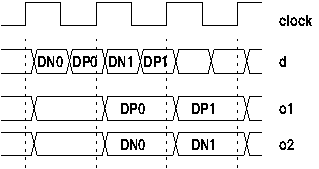
\includegraphics{iddr1}
            
            mode == "pfirst" - this is the same as above but there is an
            additional pipeline register inserted before the positive edge
            register. The two outputs thus capture +ve:-ve pairs in that order
            and both outputs are clocked on the +ve clock edge. There is an
            extra cycle of latency in this mode.
            
            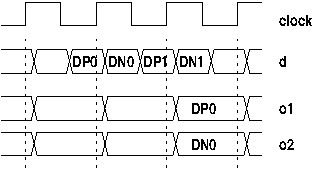
\includegraphics{iddr2}
            
            mode == "split" - input data is assigned to {\bf o1} on positive
            clock edges and to {\bf o2} on negative clock edges. The two outputs
            are thus in different (complementary) clock domains.
            
            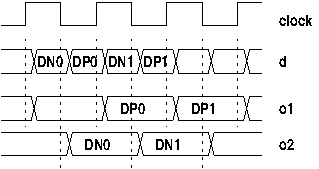
\includegraphics{iddr3}
            
            No input parameters may contain queue reads.
            
            Example code; input from a 2-channel DDR analog to digital
            converter -
            io.3pl
            \begin{lstlisting}[gobble=12, language=threepl]
               str(lvcmos33, "LVCMOS33");

               // package pins
               iopins(adc_clk_pin, lvcmos33, "str", "E17");
               iopins(adc_pins, lvcmos33, "[8]str",
                                   {"F2", "G2", "H2", "J2", "H1", "E1", "G1", "E2"});

               // ADC clock
               clock(adc_clk_in, frequency=100.0e6, loc=adc_clk_pin, ibufg=true);
               clock({global.adc_clk, adc_clk_raw}, frequency=100.0e6);
               clkdcm(clk0=adc_clk_raw <- clkin=adc_clk_in, clkfb=adc_clk);
               clockbufg(adc_clk <- adc_clk_raw);
               attributes(adc_clk, tnm="ADC_CLK");

               // ADC interface
               useclock(adc_clk);
               value({adc0, adc1}, "uint:8");
               input(adc_in, "uint:8", loc=adc_pins);
               iddr(adc0, adc1 <- adc_in,,, "nfirst");
            \end{lstlisting}
            
            Value variables {\bf adc0} and {\bf adc1} now 'point' to registers
            which are assigned ADC values on each positive edge of the clock,
            one from each channel.
            


        \subsubsection{idelay - input data delay}\label{sec:lpidelay}

            {\bf Library: xilinx/io.3pl}

            {\bf Prototype:} \\
            \vsp
            \begin{lstlisting}[gobble=12, language=threepl]
               global procedure
               idelay (
                   value(o)
                   <-
                   input(d),
                   int(delay),
                   clock(refclk),
                   value({ce, inc, rst}, "log"),
                   log(isclock)
               ) {}
            \end{lstlisting}

            {\bf Output parameters:} \\
            {\bf o} is the data output.

            {\bf Input parameters:} \\            
            {\bf d} is the data input.\\
            {\bf delay} gives a delay count.\\
            {\bf refclk} is a reference clock to control the delay.\\
            {\bf ce} is an optional clock enable for changing the delay.\\
            {\bf inc} is an optional direction control for changing the delay.\\
            {\bf rst} is an optional reset for the delay.\\
            {\bf isclock} should be true for a clock signal and false for a data
            signal.\\
         
            {\bf In-line target execution:} \\
            no

            {\bf description:} \\
            This procedure generates an input delay block.
            
            The data input {\bf d} is an input mode variable and must be a
            single bit.

            The output parameter {\bf o} is the delayed signal and is also a
            single bit.
            
            {\bf ce}, {\bf inc} and {\bf rst} inputs are used to change the
            delay value. These must be in the current clock domain.
            
            If input parameters {\bf delay} or {\bf ce} have an argument then
            the input parameter {\bf refclk} must be supplied with a clock whose
            frequency lies between 190.0MHz and 210.0MHz but is ideally 200MHz.
            If {\bf idelay()} is called more than once when {\bf variable} has
            an argument, then the same reference clock must be supplied to each
            call. Any calls to {\bf iodelay()} must also use the same reference
            clock.
            
            If input parameter {\bf ce} has no argument then the delay will be
            fixed. Input parameter {\bf delay} gives the required delay. The
            delay is $400 + 78 * delay$ pS for a reference clock frequency of
            200MHz. If {\bf delay} has no argument the delay count will be zero
            (giving $400$pS).
            
            If input parameter {\bf ce} has an argument then the delay will be
            variable. Input parameter {\bf delay} gives the initial delay count
            (default 0). The delay can be changed by asserting {\bf ce}. If {\bf
            inc} is true the delay will be incremented, otherwise it will be
            decremented. If {\bf rst} is asserted the delay will be changed back
            to the initial delay value. The clock domain of {\bf ce}, {\bf inc}
            and {\bf rst} is the current clock domain.
            
            Parameter {\bf isclock} describes the signal type which optimises
            the timing analyser for periodic or non-periodic signals.
            
            No input parameters may contain queue reads.
            
            Implementation note: this procedure will automatically create an
            IDELAYCTRL block on the first call to {\bf idelay()} that has a
            non-default delay. The Xilinx software will duplicate this across
            all locations where required. Xilinx recommend explicitly creating
            an IDELAYCTRL for each I/O region. This seems like hard work
            requiring a detailed floor plan and it is not clear why they suggest
            doing so.
            


        \subsubsection{iodelay - input/output data delay}\label{sec:lpiodelay}

            {\bf Library: xilinx/io.3pl}

            {\bf Prototype:} \\
            \vsp
            \begin{lstlisting}[gobble=12, language=threepl]
               global procedure
               iodelay (
                   value(dataout)
                   <-
                   input(idatain),
                   value(odatain),
                   log(variable),
                   int({idelay, odelay}),
                   clock(refclk),
                   value({t, ce, inc, rst}, "log")
               ) {}
            \end{lstlisting}

            {\bf Output parameters:} \\
            {\bf dataout} is the data output.

            {\bf Input parameters:} \\            
            {\bf idatain} is the data input from an IBUF (input mode variable).\\
            {\bf odatain} is the data input from OLOGIC.\\
            {\bf variable} specifies the type of input delay.\\
            {\bf idelay} gives the input delay count.\\
            {\bf odelay} gives the output delay count.\\
            {\bf refclk} is a reference clock to control the delays.\\
            {\bf t} is 3-state output control.\\
            {\bf ce} is an optional clock enable for changing the delay.\\
            {\bf inc} is an optional direction control for changing the delay.\\
            {\bf rst} is an optional reset for the delay.
        
            {\bf In-line target execution:} \\
            no

            {\bf description:} \\
            This procedure generates an input and output delay block.
            
            {\bf idatain} is an input mode variable and is the delay data
            source on input ({\bf t} is true). It must be one bit.

            {\bf odatain} is the delay data source on output ({\bf t} is false).
            This may be a CLB source ({\bf value} or {\bf static} mode variable)
            or the output of an ODDR block (output argument of oddr()). If this
            is a static mode variable it will be placed in an OLOGIC block. It must
            be a single bit.

            {\bf t} switches between input and output mode and must also control
            the output 3-state drive via an output mode variable with
            conditional assignment using {\bf t}.

            The output parameter {\bf o} is the delayed signal. It can be used
            directly or connected to an IDDR block (input argument to iddr())
            and must also be connected to an OBUFT (via an {\bf output} mode
            variable).

            If input parameter {\bf variable} is not given an argument then the
            input delay is the default fixed delay necessary for zero hold time
            on registered input data when no DCM is used. Arguments {\bf ce},
            {\bf inc} and {\bf rst} must be omitted.

            Input parameter {/bf refclk} must be supplied with a clock whose
            frequency lies between 190.0MHz and 210.0MHz but is ideally 200MHz.
            Multiple calls to {\bf iodelay()} must use the same reference clock.
            Any calls to {\bf idelay()} where parameter {\bf variable} has an
            argument must also use this same reference clock.

            If input parameter {\bf variable} has an argument whose value is
            false then the input delay will be fixed. Input parameter {\bf
            idelay} gives the required delay. The delay is $400 + 78 * delay$ pS
            for a reference clock frequency of 200MHz. If {\bf idelay} has no
            argument the delay count will be zero (giving $400$pS).

            If input parameter {\bf variable} has an argument whose value is
            true then the input delay will be variable. Input parameter {\bf
            idelay} gives the initial delay count (default 0). The delay can be
            changed by asserting {\bf ce}. If {\bf inc} is true the input delay
            will be incremented, otherwise it will be decremented. If {\bf rst}
            is asserted the input delay will be changed back to the initial
            delay value. The clock domain of {\bf ce}, {\bf inc} and {\bf rst}
            is the current clock domain.

            The output delay is set by {\bf odelay} and is $400 + 78 * delay$ pS
            for a reference clock frequency of 200MHz. If {\bf odelay} has no
            argument the delay count will be zero (giving $400$pS).

            No input parameters may contain queue reads.

            Implementation note: this procedure will automatically create an
            IDELAYCTRL block on the first call to {\bf iodelay()} that has a
            non-default delay. The Xilinx software will duplicate this across
            all locations where required. Xilinx recommend explicitly creating
            an IDELAYCTRL for each I/O region. This seems like hard work
            requiring a detailed floor plan and it is not clear why they suggest
            doing so.




        \subsubsection{iserdes - input deserialiser}\label{sec:lpiserdes}

            {\bf Library: xilinx/io.3pl}

            {\bf Prototype:} \\
            \vsp
            \begin{lstlisting}[gobble=12, language=threepl]
               global module
               iserdes (
                   value(q),
                   value({shiftout1, shiftout2}, "log")
                   <-
                   str(interface, "NETWORKING"),
                   log(master, true), log(ddr, true),
                   int(width),
                   clock({clk, clkb, oclk, oclkb, clkdiv}), value({din, ddlyin}),
                   value(bitslip, "log", false),
                   value({ce1, ce2}, "log"),
                   value({shiftin1, shiftin2, rst}, "log", false)
               ) {}
            \end{lstlisting}

            {\bf Output parameters:} \\
            see below.

            {\bf Input parameters:} \\            
            See below.
        
            {\bf In-line target execution:} \\
            no

            {\bf description:} \\
            A serial to parallel converter interface for the Xilinx
            ISERDES element. These may be used as a master-slave pair
            in DDR mode for output widths greater than 8.
            
            {\bf q} is the data output and must be of type "[n]bits:1"
            where 'n' is the output width. For a master ISERDES 'n' will be
            2, 3, 4, 5, 6, 7 or 8. For a slave ISERDES  'n' will be 2 for a
            data width of 10, or 6 for a data width of 14.
            
            {\bf shiftout1} and {\bf shiftout2} are connections to the
            slave ISERDES for widths 10 and 14.
            
            {\bf interface} selects the interface type which can be "MEMORY",
            "MEMORY\_DDR3", "MEMORY\_QDR", "OVERSAMPLE" or "NETWORKING" (default).
            
            {\bf master} selects master mode if true, or slave mode otherwise.
            Default is true (master mode)
            
            {\bf ddr} selects DDR mode if true, SDR mode if false.
            Default is true (DDR mode).
            
            {\bf width} is the data width.
            
            \begin{tabular}{| l | l | l |}
            \hline
                & networking          & memory \\
            \hline \hline
            sdc & 2, 3, 4, 5, 6, 7, 8 & not allowed \\ \hline
            ddr & 4, 6, 8, 10, 14(*)  & 4           \\ \hline
            \end{tabular}

            (* ddr mode networking interface width 14 not allowed for XC5V
            ISERDES\_NODELAY).
            
            Where a master-slave pair are used for a width of 10 or 14 that
            width argument must be the full width for both modules of the pair
            even though the data outputs {\bf q} are smaller, i.e. for a data
            width of 14 both ISERDES modules will have a width argument 14 even
            though the master has an 8-bit output and the slave a 6-bit output.
            
            {\bf clk} the main or only serial data input clock.
            
            {\bf clkb} second serial data input clock for MEMORY\_QDR mode. For
            other modes this should be the inverted main clock.
            
            {\bf oclk} is the strobe clock for memory mode.
            
            {\bf oclkb} is the inverted {\bf oclk}.
            
            {\bf clkdiv} is the frame clock input which must have a frequency
            which is serial clock frequency divided by the serial frame
            length.
            
            {\bf din} is the serial data input direct from an input pad. {\bf
            ddlyin} is the serial data input from an IDELAY element. One and
            only one of these should be given an argument.
            
            {\bf bitslip} when asserted increases the deserialiser frame
            delay by one bit position.
            
            {\bf ce1} is the clock enable for {\bf clk}.
            
            {\bf ce2} is the clock enable for {\bf clkb}.
            
            {\bf shiftin1}, {\bf shiftin2} are connections from a
            master ISERDES to a slave ISERDES for widths 10 and 14.
            
            {\bf rst} is a reset signal.
            
            See the Xilinx documentation for details on the use of this
            element.





        \subsubsection{oddr - output double data rate interface}\label{sec:lpoddr}

            {\bf Library: xilinx/io.3pl}

            {\bf Prototype:} \\
            \vsp
            \begin{lstlisting}[gobble=12, language=threepl]
               global procedure
               oddr (
                   value(o)
                   <-
                   value(i1),
                   value(i2),
                   value({ce, s, r}, "log")
               ) {}
            \end{lstlisting}

            {\bf Output parameters:} \\
            {\bf o} is the DDR data output.

            {\bf Input parameters:} \\            
            {\bf i1} is the -ve edge data input.\\
            {\bf i2} is the +ve edge data input.\\
            {\bf ce} is an optional clock enable.\\
            {\bf r} is an optional reset.\\
            {\bf s} is an optional set.
        
            {\bf In-line target execution:} \\
            no

            {\bf description:} \\
            This procedure creates an output DDR (Double Data Rate) interface.
            
            The argument to output parameter {\bf o} would usually also be
            passed as the third argument to an {\bf output()} inbuilt procedure
            call to drive output buffers.
            
            Input parameters {\bf i1} and {\bf i2} are registered on the
            current clock positive edge. The data from i1 appears at the
            output o following a positive clock edge and the data from
            i2 appears at the output o on the next negative clock edge.

            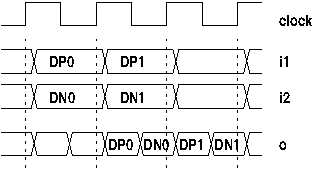
\includegraphics{oddr}
            
            The clock used for the DDR registers is the current clock.
            
            {\bf ce} is an optional clock enable.
            
            {\bf r} can be used to clear the output register and {\bf s} to set
            it to all ones. These can be synchronous or asynchronous depending
            on attribute SRTYPE and are synchronous by default.
            
            No input parameters may contain queue reads.
            
            Example; DDR output, including a clock -

            \begin{lstlisting}[gobble=12, language=threepl]
               str(lvcmos33, "LVCMOS33");

               // package pins
               iopins(out_pins, lvcmos33, "[8]str",
                                   {"F2", "G2", "H2", "J2", "H1", "E1", "G1", "E2"});
               iopins(ddr_clk_pin, lvcmos33, "str", "E17");

               static({out0, out1}, "uint:8");
               
               out0 <- .....;
               out1 <- .....;
               
               value(ddr, "uint:8");
               value(ddr_clk, "log");
               
               oddr(ddr <- out0, out1);
               oddr(ddr_clk <- false, true);
               
               output(,, ddr, loc=out_pins);
               output(,, ddr_clk, loc=ddr_clk_pin);
            \end{lstlisting}
            
            Forwarding a clock via a DDR output is a scheme suggested by
            Xilinx (XAPP 853, p9) to maintain matching phase.



        \subsubsection{oserdes - output serialiser/deserialiser}\label{sec:lposerdes}

            {\bf Library: xilinx/io.3pl}

            {\bf NOT YET IMPLEMENTED!}




    \subsection{library functions}
    
        None.





    \subsection{library classes}
    
        None.


\pagebreak

\section{Xilinx VirtexII Pro MGT library - xilinx/mgt.3pl}

    \index{library!xilinx/mgt.3pl}
    This library provide a simple 16 bit interface to a VirtexII Pro
    Multi-Gigabit Transceiver (referred to as an MGT or Rocket).
    
    This library must be incorporated by using a module statement, e.g. -
    \begin{lstlisting}[gobble=4, language=threepl]
       module "xilinx/mgt.3pl"
    \end{lstlisting}
    
    The global structures {\bf mgt\_16}, {\bf mgt\_16\_e} and {\bf mgt\_16\_ee}
    are created. They are defined as follows -

    \begin{lstlisting}[gobble=4, language=threepl]
       struct(global.gt_16,
           data,   "bits:16",  // data
           k,      "log",      // true if top 8 bits of data form a K-character
           contin, "log"       // this is a continuation word
       );
    \end{lstlisting}

    \begin{lstlisting}[gobble=4, language=threepl]
       struct(global.gt_16_e,
           data,   "bits:16",  // data
           k,      "log",      // true if top 8 bits of data form a K-character
           first,  "log",      // previous word was an idle
           error,  "log"       // disparity error or not-in-table error
       );
    \end{lstlisting}

    \begin{lstlisting}[gobble=4, language=threepl]
       struct(global.gt_16_ee,
           data,       "bits:16",  // data
           k,          "log",      // true if top 8 bits of data form a K-character
           first,      "log",      // previous word was an idle
           disperr,    "[2]log",   // disparity errors
           niterr,     "[2]log"    // not-in-table errors
       );
    \end{lstlisting}

    {\bf mgt\_16} is used for input data. {\bf mgt\_16\_e} and
    {\bf mgt\_16\_ee} are used for output data, the former providing a simpler
    error indication than the latter.
    
    The global structure {\bf ds16} is also used and it is created in
    {\bf stdlib.3pl}. It is 
    \begin{lstlisting}[gobble=4, language=threepl]
       struct(global.ds16,
           data,   "bits:16",  // data
           k,      "log"       // true if top 8 bits of data form a K-character
       );
    \end{lstlisting}


    \subsection{library modules}

        \subsubsection{gt\_custom\_16 - a 16-bit Rocket high-speed serial I/O channel}\label{sec:lmgtcustom16}

            {\bf Library: xilinx/mgt.3pl}

            {\bf Prototype:} \\
            \vsp
            \begin{lstlisting}[gobble=12, language=threepl]
               global module
                   gt_custom_16 (
                       queue(out),
                       clock(ruclk),
                       value(rxdiag, "[5]log"),
                       value(txdiag, "[2]log")
                       <-
                       str({loc, txp_pin, txn_pin, rxp_pin, rxn_pin, clkp_pin, clkn_pin}),
                       float(freq),         // MGT base frequency
                       queue(in),
                       int(run_length),
                       value(reset, "log"),
                       int(tx_diff_ctrl, 500),
                       int(tx_preemphasis, 0),
                       value(loopback, "uint:2", 0),
                       log(los_fsm)
                   ) {}
            \end{lstlisting}

            {\bf Output parameters:} \\
            {\bf out} is the data output.\\
            {\bf ruclk} is the user interface clock.\\
            {\bf rxdiag} provides five diagnostic receiver signals.\\
            {\bf txdiag} provides two diagnostic transmitter signals.

            {\bf Input parameters:} \\
            {\bf loc} gives the MGT location coordinates.\\
            {\bf txp\_pin} specifies the transmitter positive output pin.\\
            {\bf txn\_pin} specifies the transmitter negative output pin.\\
            {\bf rxp\_pin} specifies the receiver positive input pin.\\
            {\bf rxn\_pin} specifies the receiver negative input pin.\\
            {\bf clkp\_pin} specifies the clock input positive pin.\\
            {\bf clkn\_pin} specifies the clock input negative pin.\\
            {\bf freq} is the parallel input and output data frequency.\\
            {\bf in} is the data input.\\
            {\bf run\_length} is the maximum data run length.\\
            {\bf reset} when true resets the initialisation flag.\\
            {\bf tx\_diff\_ctrl} specifies the differential output voltage.\\
            {\bf tx\_preemphasis} specifies the transmitter preemphasis.\\
            {\bf loopback} when true connects the MGT in loopback mode.\\
            {\bf los\_fsm} when true connects enables the MGT loss-of-sync FSM.

            {\bf Description:} \\
            This module provides a simple interface to procedure
            {\bf mgt()} \autorefph{sec:lpmgt}, in this library.
            It creates both an input and an output interface to the
            VirtexII Pro MGT. The data width is 16 bit. A custom protocol
            is used. 
            
            The particular MGT is selected by the first 7 input arguments.
            The {\bf loc} does not seem to be required but the transmitter pin,
            receiever pin and clock pin pairs must be provided. The following
            combinations apply to the XC2VP4 -           
            
            \begin{tabular}{| l || r | r | r | r |}
            \hline
            MGT      & TXP  & TXN  & RXP  & RXN  \\
            location & pin  & pin  & pin  & pin  \\
            \hline
            \hline
            GT\_X0Y0 & AB8  & AB7  & AB9  & AB10 \\
            \hline
            GT\_X0Y1 & A8   & A7   & A9   & A10  \\
            \hline
            GT\_X1Y0 & AB14 & AB13 & AB15 & AB16 \\
            \hline
            GT\_X1Y1 & A14  & A13  & A15  & A16  \\
            \hline
            \end{tabular}
            
            and for the XC2VP40 -

            \begin{tabular}{| l || r | r | r | r |}
            \hline
            MGT      & TXP  & TXN  & RXP  & RXN  \\
            location & pin  & pin  & pin  & pin  \\
            \hline
            \hline
            GT\_X0Y0 & ap32 & ap33 & ap31 & ap30 \\
            \hline
            GT\_X0Y1 &  a32 &  a33 &  a31 &  a30 \\
            \hline
            GT\_X1Y0 & ap28 & ap29 & ap27 & ap26 \\
            \hline
            GT\_X1Y1 &  a28 &  a29 &  a27 &  a26 \\
            \hline
            GT\_X2Y0 & ap20 & ap21 & ap19 & ap18 \\
            \hline
            GT\_X2Y1 &  a20 &  a21 &  a19 &  a18 \\
            \hline
            GT\_X3Y0 & ap16 & ap17 & ap15 & ap14 \\
            \hline
            GT\_X3Y1 &  a16 &  a17 &  a15 &  a14 \\
            \hline
            GT\_X4Y0 &  ap8 &  ap9 &  ap7 &  ap6 \\
            \hline
            GT\_X4Y1 &   a8 &   a9 &   a7 &   a6 \\
            \hline
            GT\_X5Y0 &  ap4 &  ap5 &  ap3 &  ap2 \\
            \hline
            GT\_X5Y1 &   a4 &   a5 &   a3 &   a2 \\
            \hline
            \end{tabular}
            
            {\bf freq} is an immediate floating point value which specifies the
            MGT base frequency in Hz. For 2.5GHz serial the base frequency
            is 125.0MHz (serial rate divided by 20).
            
            Input parameter {\bf in} is the input data queue for the transmitter.
            If the transmitter is not used the argument is omitted. The type is
            either the struct {\bf ds16} (defined in stdlib.3pl) or the struct
            {\bf gt\_16}. The most significant byte of the word may be a
            K-character, which is signified by setting field {\bf k} true. The
            byte must be one of the allowed K-characters (this is not checked!).
            For type {\bf gt\_16} the {\bf contin} field should be true if this
            word is a continuation word, i.e. it is not the first word in a
            block. This ensures that despite the run length constraint (see
            Input parameter {\bf run\_length} below) a block will not be split
            by inserted idles. At the receiving end the first word following an
            idle can reset a block boundary.

            Input parameter {\bf run\_length} is an immediate integer which
            specifies the maximum contiguous data run for the transmitter. If
            data input is continuously available such that this length would be
            exceeded (and the data {\bf contin} field is not true - see above)
            then an idle sequence is inserted in the output stream. When no data
            are available for transmission a continuous stream of idles is
            transmitted. These idles are used by the receiver to lock initially
            and to continue checking that lock is maintained. If receiver lock
            is lost then lock can only be regained at the next idle. In the
            custom protocol used in this interface the idle sequence is a single
            16-bit word containing a comma byte. If no argument is supplied
            to parameter {\bf run\_length} then idles will only be inserted
            when the input queue is unavailable.

            Input parameter {\bf reset} is used to clear the initialisation flag
            and execute initialisation process. This initialisation process
            expects to receive idles only for 6 seconds without error. If an
            error or a non-idle word is received in this time the received is
            reset and a further wait ensues. When 6 seconds of idles have been
            received the initialisation flag is set and the channel can now receive
            data. The initialisation process occurs immediately following
            configuration of the FGA. Clearly during this initialisation, and any
            others that are explicitly induced, the transmitter must be sending
            idles.

            Input parameter {\bf tx\_diff\_ctrl} specifies the differential
            output voltage and is 500 by default. Values are 400, 500, 600, 700
            or 800 which is the differential voltage in mV. The peak-to-peak
            voltage is twice this figure.

            Input parameter {\bf tx\_preemphasis} specifies the transmitter
            preemphasis and is 0 by default. values are 0 (10\%), 1 (20\%),
            2 (25\%) or 3 (33\%).

            Input parameters {\bf tx\_diff\_ctrl} and {\bf tx\_preemphasis} control
            the transmitter output waveforms to correct for different cable types
            and lengths. Any changes to the default values are usually done
            empirically based on the measured error rate.

            Input parameter {\bf loopback} is an immediate integer which specifies
            the loopback mode. If the argument is omitted or is 0, operation is
            normal, i.e. loopback is not connected. Value 1 specifies internal
            parallel mode. Value 2 specifies internal serial mode.
            
            Input parameter {\bf los\_fsm} controls the use of the MGT loss-of-sync
            finite state machine which detects when sync is held/lost. If the argument
            to this is false then {\bf rxdiag[3]} will only indicate if channel
            initialisation was successful. If {\bf los\_fsm} is true then  {\bf
            rxdiag[3]} will be asserted when the receiver has been successfully
            initialised and remain asserted while sync is OK.

            Output parameter {\bf out} is the output data queue for the receiver.
            If the receiver is not used the argument is omitted. The type can be
            struct {\bf ds16}, struct {\bf gt\_16\_e} or  struct {\bf
            gt\_16\_ee} depending on the level of error
            detail required. The {\bf k} field in each case is true if the most
            significant byte of the received word contains a K-character.
            For {\bf gt\_16\_e} or  {\bf gt\_16\_ee} the {\bf first} field
            is true then this word follows an idle, which information may be
            used to reset a block boundary. {\bf Important note - the output
            queue must not block! The destination module must read it at a rate
            that precludes it ever becoming full, if necessary reading it to
            null. Generally the read clock domain must have an equal or higher
            frequency than the user interface clock {\bf ruclk}, but this may be
            relaxed if it is known that the serial data source has a guaranteed
            maximum data rate that would allow a lower queue read clock domain.}
            For {\bf gt\_16\_e} the {\bf error} field is true if either byte
            exhibits a disparity error or not-in-table error. {\bf gt\_16\_ee}
            provides each of these errors separately for each byte.
            
            A word in which a disparity error or a not-in-table error occurs is
            written to the output queue but the error field is true. If the top
            byte of a word is a K-character the {\bf k} field is true.

            Output parameter {\bf ruclk} is the user interface clock at the base
            frequency.
            
            Output parameter {\bf rxdiag} provides five diagnostic outputs for the
            receiver. These are -
            \blist
            \item   diag[0] - rxcommadet, which is true when a positive or
                    negative comma is being received
            \item   diag[1] - rxdisperr[0] or rxnotintable[0], which is true
                    when a disparity error or a not-in-table error is
                    flagged for the current upper byte of the 16-bit output
            \item   diag[2] - rxdisperr[1] or rxnotintable[1], which is true
                    when a disparity error or a not-in-table error is
                    flagged for the current lower byte of the 16-bit output
            \item   diag[3] - is true if the receiver is synchronised, as
                    indicated by the receiver synchronisation FSM \footnote{if
                    parameter los\_fsm is true.} , and the
                    initialisation flag is high
            \item   diag[4] - is true if the receiver is receiving idles
            \blend
            These outputs might be connected to status LEDs to indicate that the
            receiver is locked and functioning correctly. {\bf diag[0]} will be true
            while the receiver is receiving idles but will be false when data are
            received.

            Output parameter {\bf txdiag} provides two diagnostic outputs for the
            transmitter. These are -
            \blist
            \item   diag[0] - is true if the transmitter is sending idles
            \item   diag[1] - is true if the transmitter is sending a word in which
                    the top byte is a control character
            \blend


    \subsection{library procedures}

        \subsubsection{mgt - create an MGT high-speed serial I/O channel}\label{sec:lpmgt}

            {\bf Library: xilinx/mgt.3pl}

            {\bf Prototype:} \\
            \vsp
            \begin{lstlisting}[gobble=12, language=threepl]
               global procedure
               mgt (
                   // outputs
                   value(rxdata),
                   value(rxchariscomma, "[]log"),
                   value(rxcharisk, "[]log"),
                   value(rxcommadet, "log"),
                   value(rxlossofsync, "uint:2"),
                   value(rxnotintable, "[]log"),
                   value(rxbufstatus, "[2]log"),
                   value(rxcheckingcrc, "log"),
                   value(rxclkcorcnt, "uint:3"),
                   value(rxcrcerr, "log"),
                   value(rxdisperr, "[]log"),
                   value(rxrealign, "log"),
                   value(rxrecclk, "log"),
                   value(rxrundisp, "[]log"),
                   value(txbuferr, "log"),
                   value(txkerr, "[]log"),
                   value(txrundisp, "[]log"),
                   value(chbondo, "[4]log"),
                   value(chbonddone, "log")
                   <-
                   // attributes
                   str(loc),
                   str(txn_pin),
                   str(txp_pin),
                   str(rxn_pin),
                   str(rxp_pin),
                   log(align_comma_msb),
                   int(chan_bond_limit),
                   str(chan_bond_mode),
                   int(chan_bond_offset),
                   log(chan_bond_one_shot),
                   int(chan_bond_seq_1_1),
                   int(chan_bond_seq_1_2),
                   int(chan_bond_seq_1_3),
                   int(chan_bond_seq_1_4),
                   int(chan_bond_seq_2_1),
                   int(chan_bond_seq_2_2),
                   int(chan_bond_seq_2_3),
                   int(chan_bond_seq_2_4),
                   log(chan_bond_seq_2_use),
                   int(chan_bond_seq_len),
                   int(chan_bond_wait),
                   log(clk_cor_insert_idle_flag),
                   log(clk_cor_keep_idle),
                   int(clk_cor_repeat_wait),
                   int(clk_cor_seq_1_1),
                   int(clk_cor_seq_1_2),
                   int(clk_cor_seq_1_3),
                   int(clk_cor_seq_1_4),
                   int(clk_cor_seq_2_1),
                   int(clk_cor_seq_2_2),
                   int(clk_cor_seq_2_3),
                   int(clk_cor_seq_2_4),
                   log(clk_cor_seq_2_use),
                   int(clk_cor_seq_len),
                   log(clk_correct_use),
                   int(comma_10b_mask),
                   int(crc_end_of_pkt),
                   str(crc_format),
                   int(crc_start_of_pkt),
                   log(dec_mcomma_detect),
                   log(dec_pcomma_detect),
                   log(dec_valid_comma_only),
                   int(mcomma_10b_value),
                   log(mcomma_detect),
                   int(pcomma_10b_value),
                   log(pcomma_detect),
                   int(ref_clk_v_sel),
                   log(rx_crc_use),
                   int(rx_data_width),
                   log(rx_decode_use),
                   int(rx_los_invalid_incr),
                   int(rx_los_threshold),
                   log(rx_loss_of_sync_fsm),
                   log(serdes_10b),
                   int(termination_imp),
                   int(tx_crc_force_value),
                   log(tx_crc_use),
                   int(tx_data_width),
                   int(tx_diff_ctrl),
                   int(tx_preemphasis),
                   // Inputs
                   value(chbondi, "[4]log"),
                   value(enchansync, "log"),
                   value(enmcommaalign, "log"),
                   value(enpcommaalign, "log"),
                   value(loopback, "uint:2"),
                   value(powerdown, "log"),
                   value(refclk, "log"),
                   value(refclk2, "log"),
                   value(brefclk, "log"),
                   value(brefclk2, "log"),
                   value(refclksel, "log"),
                   value(rxpolarity, "log"),
                   value(rxreset, "log"),
                   clock(rxusrclk),
                   clock(rxusrclk2),
                   value(txbypass8b10b, "[]log"),
                   value(txchardispmode, "[]log"),
                   value(txchardispval, "[]log"),
                   value(txcharisk, "[]log"),
                   value(txdata),
                   value(txforcecrcerr, "log"),
                   value(txinhibit, "log"),
                   value(txpolarity, "log"),
                   value(txreset, "log"),
                   clock(txusrclk),
                   clock(txusrclk2)

               ) {}
            \end{lstlisting}

            {\bf Output parameters:} \\
            See Xilinx documentation.

            {\bf Input parameters:} \\
            See Xilinx documentation.

            {\bf In-line target execution:} \\
            no

            {\bf description:} \\
            This procedure creates an MGT high speed serial I/O channel.
            For a simpler interface
            see {\bf gt\_custom\_16} \autorefph{sec:lmgtcustom16} above.



    \subsection{library functions}
    
        None.


    \subsection{library classes}
    
        None.


\pagebreak

\section{Xilinx netlist postprocessing module - xilinx/postprocess.3pl}\label{ch:pp}

    \index{library!xilinx/postprocess.3pl}
    This module converts the EDIF netlist produced by 3PL to a configuration
    file. It has a single procedure.
    
    This library must be incorporated by using a postmodule statement, e.g. -
    \begin{lstlisting}[gobble=4, language=threepl]
       postmodule ("xilinx/postprocess.3pl");
    \end{lstlisting}
    
    See \autorefph{sec:mpfcdecl} and \autorefph{sec:xpp}.
    
    More than one postprocessing module can be specified in which case an
    additional integer argument can be supplied to specify ordering. If omitted
    the order in which the modules have been added to the list will be the order
    of execution. Thus far only this module has been used.
    


    \subsection{library modules}

        None.



    \subsection{library procedures}

        \subsubsection{postprocess - post-process the netlist file}\label{sec:lppostprocess}

            {\bf Prototype:} \\
            \vsp
            \begin{lstlisting}[gobble=12, language=threepl]
                global procedure
                postprocess(
                    str(rname),
                    str(tool),
                    float(minver, 1.0),
                    float(maxver, 9999.0)
                ) {}
            \end{lstlisting}



            {\bf Output parameters:} \\
            
            None.

            {\bf Input parameters:} \\
            \begin{tabular}{| l | l | l | l |}
            \hline
                            & mode      & type   & \\
            \hline \hline
            {\bf rname}     & immediate & str    & optional file name for recipe file \\ \hline
            {\bf tool}      & immed     & str    & "ise" or "vivado" \\ \hline
            {\bf minver}    & immediate & float  & minimum version number  \\ \hline
            {\bf maxver}    & immediate & float  & maximum version number \\ \hline
            \end{tabular}

            {\bf In-line target execution:} \\
            no

            {\bf description:} \\
            This procedure executes the Xilinx place-and-route tools to
            generate the configuration bit file from the EDIF netlist file
            produced by 3PL. To do this it executes the Xilinx tools
            on the host CPU via calls to exec().
            
            {\bf rname} optional and is the name of a file containing a recipe
            of commands. If supplied it overrides the recipe file specified by
            directive {\bf postProcessRecipe}. Recipe files
            {\bf ise\_cpld.cmd}, {\bf ise\_fpga.cmd}, {\bf ise\_xflow.cmd}
            and {\bf vivado.tcl} are available in the directory
            containing postprocess.3pl.
            
            {\bf tool} "ise" or "vivado" must be supplied and specifies the
            main place-and-route tool to be used.
            
            If directives {\bf XILINX\_ISE} or {\bf XILINX\_VIVADO} are supplied
            (as appropriate to the platform) then this specifies the specific
            path of the place-and-route tool to execute. Otherwise the path
            specified by directive {\bf XILINX} will be used along with  {\bf
            minver} and {\bf maxver} to select the specific version of the ISE
            or Vivado software. The highest version \verb'>=' minver and
            \verb'<=' maxver will be used.


            if directive {\bf postProcessAppendFile} exists it specifies
            a file to append to the bit file, usually a .info file

            if directive {\bf postProcessCompress} exists and is true
            the bit file will be compressed.

            If directive {\bf postProcessFilter} exists it specifies that the
            standard output from the place-and-route tools should be filtered.
            Values may be -
            \blist
            \item   "error" - lines starting with "ERROR" are retained
            \item   "critical" - the above plus lines starting with "CRITICAL" are
                    retained
            \item   "warning" - the above plus lines starting with "WARNING" are
                    retained
            \item   "info" - the above plus lines starting with "INFO" are
                    retained
            \blend
            any other values being ignored. If this directive is not defined or
            has an invalid value then no filtering is applied.
    
    
    


    \subsection{library functions}
    
        None.


    \subsection{library classes}
    
        None.


\pagebreak

\section{Embedded PowerPC Interface Library - xilinx/ppc405lib.3pl}
\label{chap:lmppc405lib}

    {\bf This library has never been used in earnest so its functionality has not
    been tested!}

    \index{library!xilinx/ppc405lib.3pl}
    {\bf This library provides an instantiation of an embedded PowerPC.}
    
    This library must be incorporated by using a {\bf module} statement -
    \begin{lstlisting}[gobble=4, language=threepl]
       module "xilinx/ppc405lib.3pl"
    \end{lstlisting}




    \subsection{library modules}
    
    None.



    \subsection{library procedures}

         \subsubsection{ppc405 - a PPC405}\label{sec:lpppc405}

            {\bf Library: xilinx/ppc405lib.3pl}

            {\bf Prototype:} \\
            \vsp
            \begin{lstlisting}[gobble=12, language=threepl]
               global procedure
               ppc405 (
                   value({ C405CPMCORESLEEPREQ, C405CPMMSRCE, C405CPMMSREE, C405CPMTIMERIRQ,
                           C405CPMTIMERRESETREQ, C405DBGMSRWE, C405DBGSTOPACK,
                           C405DBGWBCOMPLETE, C405DBGWBFULL, C405DCRREAD, C405DCRWRITE,
                           C405JTGCAPTUREDR, C405JTGEXTEST, C405JTGPGMOUT, C405JTGSHIFTDR,
                           C405JTGTDO, C405JTGTDOEN, C405JTGUPDATEDR, C405PLBDCUABORT,
                           C405PLBDCUCACHEABLE, C405PLBDCUGUARDED, C405PLBDCUREQUEST,
                           C405PLBDCURNW, C405PLBDCUSIZE2, C405PLBDCUU0ATTR,
                           C405PLBDCUWRITETHRU, C405PLBICUABORT, C405PLBICUU0ATTR,
                           C405RSTCHIPRESETREQ, C405RSTCORERESETREQ, C405RSTSYSRESETREQ,
                           C405TRCCYCLE, C405PLBICUREQUEST, C405TRCTRIGGEREVENTOUT,
                           C405XXXMACHINECHECK, DSOCMBRAMEN, DSOCMBUSY, ISOCMBRAMEN,
                           ISOCMBRAMEVENWRITEEN, ISOCMBRAMODDWRITEEN, C405PLBICUCACHEABLE}, "log"),
                   value(C405DBGWBIAR, "bits:30"),
                   value(C405DCRABUS, "bits:10"),
                   value(C405DCRDBUSOUT, "bits:32"),
                   value(C405PLBDCUABUS, "bits:32"),
                   value(C405PLBDCUBE, "bits:8"),
                   value(C405PLBDCUPRIORITY, "uint:2"),
                   value(C405PLBDCUWRDBUS, "bits:64"),
                   value(C405PLBICUABUS, "uint:30"),
                   value(C405PLBICUPRIORITY, "uint:2"),
                   value(C405PLBICUSIZE, "uint:2"),
                   value(C405TRCEVENEXECUTIONSTATUS, "uint:2"),
                   value(C405TRCODDEXECUTIONSTATUS, "uint:2"),
                   value(C405TRCTRACESTATUS, "uint:4"),
                   value(C405TRCTRIGGEREVENTTYPE, "uint:11"),
                   value(DSOCMBRAMABUS, "uint:22"),
                   value(DSOCMBRAMBYTEWRITE, "[4]log"),
                   value(DSOCMBRAMWRDBUS, "bits:32"),
                   value(ISOCMBRAMRDABUS, "uint:21"),
                   value(ISOCMBRAMWRABUS, "uint:21"),
                   value(ISOCMBRAMWRDBUS, "bits:32")
                   <-
                   int({XLOC, YLOC}),
                   clock({ BRAMDSOCMCLK, BRAMISOCMCLK, CPMC405CLOCK, PLBCLK}),
                   value({ CPMC405CORECLKINACTIVE, CPMC405CPUCLKEN, CPMC405JTAGCLKEN, 
                           CPMC405TIMERCLKEN, CPMC405TIMERTICK, DBGC405DEBUGHALT,
                           DBGC405EXTBUSHOLDACK, DBGC405UNCONDDEBUGEVENT, DCRC405ACK, 
                           EICC405CRITINPUTIRQ, EICC405EXTINPUTIRQ, JTGC405BNDSCANTDO,
                           JTGC405TCK, JTGC405TDI, JTGC405TMS, JTGC405TRSTNEG,
                           MCBCPUCLKEN, MCBJTAGEN, MCBTIMEREN, MCPPCRST,
                           PLBC405DCUADDRACK, PLBC405DCUBUSY, PLBC405DCUERR, 
                           PLBC405DCURDDACK, PLBC405DCUSSIZE1, PLBC405DCUWRDACK,
                           PLBC405ICUADDRACK, PLBC405ICUBUSY, PLBC405ICUERR, 
                           PLBC405ICURDDACK, PLBC405ICUSSIZE1, RSTC405RESETCHIP, 
                           RSTC405RESETCORE, RSTC405RESETSYS, TIEC405DETERMINISTICMULT,
                           TIEC405DISOPERANDFWD, TIEC405MMUEN, TRCC405TRACEDISABLE,
                           TRCC405TRIGGEREVENTIN}, "log"),
                   value(BRAMDSOCMRDDBUS, "bits:32"),
                   value(BRAMISOCMRDDBUS, "bits:64"),
                   value(DCRC405DBUSIN, "bits:32"),
                   value(DSARCVALUE, "uint:8"),
                   value(DSCNTLVALUE, "uint:8"),
                   value(ISARCVALUE, "uint:8"),
                   value(ISCNTLVALUE, "uint:8"),
                   value(PLBC405DCURDDBUS, "bits:64"),
                   value(PLBC405DCURDWDADDR, "uint:3"),
                   value(PLBC405ICURDDBUS, "bits:64"),
                   value(PLBC405ICURDWDADDR, "uint:3"),
                   value(TIEDSOCMDCRADDR, "uint:8"),
                   value(TIEISOCMDCRADDR, "uint:8")
               ) {}
            \end{lstlisting}

            {\bf Output parameters:} \\
            See Xilinx documentation.

            {\bf Input parameters:} \\
            See Xilinx documentation.

            {\bf description:} \\
            This procedure creates an instance of a PowerPC 405 core.
            For a simpler interface see procedure {\bf ppcbr} \autorefph{sec:lpppcbr}
            above.






    \subsection{library functions}
    
    None.




    \subsection{library classes}
    
        None.


\pagebreak

\section{Embedded PowerPC Interface Library - xilinx/ppclib.3pl}
\label{chap:lmppclib}

    \index{library!xilinx/ppclib.3pl}
    {\bf This library provides a way of instantiating an embedded PowerPC. The
    library was under development but work on it has ceased. Its functionality has
    not been tested!}
    
    This library must be incorporated by using a {\bf module} statement -
    \begin{lstlisting}[gobble=4, language=threepl]
       module "xilinx/ppclib.3pl"
    \end{lstlisting}



    \subsection{library modules}
    
    None.



    \subsection{library procedures}

         \subsubsection{ppcbr - a PPC405 with OCM}\label{sec:lpppcbr}

            {\bf Library: xilinx/ppclib.3pl}

            {\bf Prototype:} \\
            \vsp
            \begin{lstlisting}[gobble=12, language=threepl]
               global module
               ppcbr (
                   var({iramp, dramp0, dramp1, dramp2, dramp3}, "->")
                   <-
                   int({imsk, dmsk}),
                   log({iramea, dramea}),
                   value({cpuclken, cpureset}, "log")
               ) {}
            \end{lstlisting}

            {\bf Output parameters:} \\
            {\bf iramp} pointer to 64 bit instruction RAM\\
            {\bf dramp0} pointer to data RAM byte 0 (most sig) \\
            {\bf dramp1} pointer to data RAM byte 1 \\
            {\bf dramp2} pointer to data RAM byte 2 \\
            {\bf dramp3} pointer to data RAM byte 3 (least sig)

            {\bf Input parameters:} \\            
            {\bf imsk} instruction memory size (bytes) in K - each 2K takes a
                       block RAM - must be 4, 8, 16, 32, 64 or 128\\           
            {\bf dmsk} data memory size (bytes) in K - each 2K takes a block RAM -
                       must be 2, 4, 8, 16, 32 or 64\\
            {\bf iramea} true if instruction ram 2nd port required for external
                         access\\
            {\bf dramea} true if data ram 2nd port required for external access\\
            {\bf cpuclken} enable CPU core clock\\
            {\bf cpureset} reset the CPU - this should be raised for a clock cycle\\

            {\bf description:} \\
            This procedure creates an interface to an embedded PowerPC 405. It
            uses on-chip block RAM for separate instruction and data memory.
            Both memories are located at address 0. The memory management is
            disabled. Pointers to the memories are available as output
            parameters to enable access via the second RAM port.
            This procedure calls {\bf ppc405} \autorefph{sec:lpppc405} above
            to create the PPC instance.
    




    \subsection{library functions}
    
        None.



    \subsection{library classes}
    
        None.




\pagebreak

\section{Zynq ARM processor interface Library - xilinx/zynq\_axi.3pl}
\label{chap:lmzynqaxilib}

    \index{library!xilinx/zynq\_axi.3pl}
    This library instantiates a Zynq CPU and provides interfaces to
    the two general purpose memory-mapped slave buses and the four
    high performance DMA master buses. It also connects the DDR RAM
    and general purpose I/O pins to the CPU.
    
    This library must be incorporated by using a {\bf source} statement -
    \begin{lstlisting}[gobble=4, language=threepl]
       source "xilinx/zynq\_axi.3pl"
    \end{lstlisting}

    however xilinx/zynq\_axi.3pl is already included in board header files -\\
    boards/avnet/microzed\_7010.3pl\\
    boards/avnet/microzed\_7020.3pl\\
    boards/digilent/zybo.3pl
    
    Code to create the interface to the CPU must be executed as a trailer module
    by -
    
    \begin{lstlisting}[gobble=4, language=threepl]
        trailermodule ("zynq processor") {
            zynq_ps();
        }
    \end{lstlisting}
    and this is also incorporated in the header files listed above.

    Application code only needs to incorporate the board header file
    and create an instance of the CPU interface, e.g. -

    \begin{lstlisting}[gobble=4, language=threepl]
        module "boards/avnet/microzed_7010.3pl"

        class(cpu, cpu_api());
    \end{lstlisting}
    The CPU\_API class is documented in
    \autorefph{chap:lmxilcpulib} {\bf FPGA to CPU interface Library
    - xilinx/cpu.3pl}. This library can also be used by FPGA boards
    which have a USB serial interface to a host computer.
   
    Since cpu.3pl is included via a source statement its code shares the scope
    of this library, UART\_CPU. Thus it can call the modules, functions and
    procedures therin.
    
    {\bf cpu.3pl} defines a class {\bf CPU\_API()} which provides the following
    class procedures for data transfer between FPGA and CPU - \\
        \hspace*{1cm}{\bf read()} generic read \autorefph{sec:lpcpurd} \\
        \hspace*{1cm}{\bf write()} generic write \autorefph{sec:lpcpuwr} \\
        \hspace*{1cm}{\bf read\_memory()} memory read \autorefph{sec:lpcpurdmem} \\
        \hspace*{1cm}{\bf read\_queue()} queue read \autorefph{sec:lpcpurdqueue} \\
        \hspace*{1cm}{\bf read\_value()} value read \autorefph{sec:lpcpurdvalue} \\
        \hspace*{1cm}{\bf write\_memory()} memory write \autorefph{sec:lpcpuwrmem} \\
        \hspace*{1cm}{\bf write\_queue()} queue write \autorefph{sec:lpcpuwrqueue} \\
        \hspace*{1cm}{\bf write\_static()} static write \autorefph{sec:lpcpuwrstat} \\
        \hspace*{1cm}{\bf dma\_read()} to FPGA from CPU \autorefph{sec:lpcpudmar} \\
        \hspace*{1cm}{\bf dma\_write()} from FPGA to CPU \autorefph{sec:lpcpudmaw} \\
        \hspace*{1cm}{\bf signal\_interrupt()} interrupt from a signal \autorefph{sec:lpcpusigint} \\
        \hspace*{1cm}{\bf interrupt()} interrupt procedure \autorefph{sec:lpcpuint} \\

    each of which can generate an instance of a CPU interface to a specific 3PL
    variable of appropriate mode. An internal class {\bf CPU\_CODEGEN} is also
    created but this is not visible to the application code 
    
    cpu.3pl is sourced by both {\bf uart\_cpu.3pl} and {\bf zynq\_axi.3pl} to
    provide CPU interfaces. The former employs a serial data link and the
    latter parallel busses.
    
    When any of the procedures above are called a defining structure is
    created which is added to a list of CPU interfaces. At the end
    of immediate execution module {\bf create\_bus\_interfaces()} is called.
    {\bf create\_bus\_interfaces()} is defined in both {\bf uart\_cpu.3pl}
    and {\bf zynq\_axi.3pl} as it is specific to each. This module
    traverses the interface list constructed above and for each interface
    calls a matching procedure in class {\bf CPU\_CODEGEN} to generate the
    logic for each instance.


    
    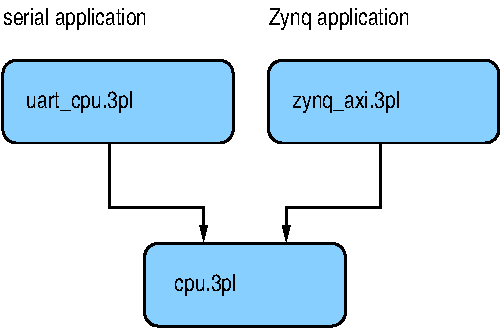
\includegraphics{cpu}
    
    Bus GP0 is used for reading 3PL expression values and queue mode variables
    and writing static and queue mode variables.

    Bus GP1 is used to read and write 3PL memory mode variables.

    For both GP buses burst transfers are used and burst lengths may be up to 8
    32-bit words. Burst transfers are executed in the CPU interface code by
    load/store multiple commands which use a contiguous set of registers. A
    maximum of 8 of the 16 available registers has been imposed, hence the
    maximum burst size of 8 32-bit words.

    An information file, design.info, is generated. This file lists the
    directives, AXI bus interface details and interrupt event parameters. The
    file is in JSON format. A python utility program, info2c,  extracts data
    from this information file and generates a .h file for CPU programs in C.
    Similar utilities may be written for other languages.

    info2c is a shell script invoking python. The first or only argument is the
    design name and info2c expects to find a file design.info. It will create a
    file design.h. If the optional second argument is provided then it is used
    as the output file name (".h" is appended).
    
    The design.info data may also be stored in block RAM (rmemory) for read-time
    access by CPU code. This is enabled by default but may be avoided via a
    directive, i.e. {\bf directive("excludeinfo", true);}, which can be executed
    at any time during 3PL immediate execution. The compression is done by
    calling inbuilt function {\bf deflate()} \autorefph{sec:ifdeflate}. The
    readback is initialised by writing to address 1 and 32-bit packed .info data
    is then read by successive 32-bit reads from address 1. The first read
    returns a 32 bit CRC-32 checksum for the remainder of the block,\. The
    second read returns the uncompressed data size in bytes and the third read
    returns the compressed data size in bytes. Reads beyond the data length will
    return zeros.
    
    The data block size depends on the size of the compressed .info data and
    varies from a minimum of 1024 32 bit words (1 RAM block) to 32,768 words (32
    RAM blocks).

    These bus interfaces allocate successive addresses. These addresses are
    embedded in C functions generated by info2c and hence the programmer does
    not need to know the addresses (they can be determined from the .info file).
    Each interface is supplied a unique name in the 3PL procedure call and this
    name is used in the associated generated function names.

    For 3PL int types info2c will generate matching C types int8\_t, int16\_t,
    int32\_t or int64\_t as appropriate to the size of the datum. The maximum
    primitive size is 64 bits.

    For 3PL uint or bits types info2c will generate matching C types uint8\_t,
    uint16\_t, uint32\_t or uint64\_t as appropriate to the size of the datum.
    The maximum primitive size is 64 bits.

    For 3PL log type info2c will generate matching type bool\_t

    For  3PL structs or enums info2c will generate a matching C bit field
    struct. The maximum size for a struct is 64 bits.

    For a 3PL float type info2c will generate a C float or double type if the
    the type matches IEEE 754 format, otherwise it will generate a C bit field
    struct containing the exponent and mantissa as fields.

    The 3PL data type may be an array of uint, bits or int of exactly 32 or 64
    bits where the dimension is a maximum of 8 for 32 bit members or 4 for 64
    bit members. The matching C type generated will be a struct containing the
    array.



    \subsection{library modules}


        \subsubsection{cpu\_write\_dma\_buffer - DMA transfer to CPU RAM}\label{sec:lmzynqdmabufr}

            {\bf Library: xilinx/zynq\_axi.3pl}

            {\bf Prototype:} \\
            \vsp
            \begin{lstlisting}[gobble=12, language=threepl]
               global module
               cpu_write_dma_buffer (
                   str(name),          // interface name
                   int(blockwords),    // block length in data words
                   int(nblocks),       // number of blocks
                   queue(in),          // data in
                   log(use_wcount),    // use queue count rather than interrupt
                   log(bigendian)      // transfer data as bigendian
               ) {}
            \end{lstlisting}

            {\bf Output parameters:} \\
            none

            {\bf Input parameters:} \\            
            {\bf name} is a string identifier for the interface.\\
            {\bf blockwords} is the DMA block length in data words.\\
            {\bf nblocks} is the number of DMA blocks used.\\
            {\bf in} is a queue of data to be transferred.\\
            {\bf use\_wcount} determines whether an interrupt or a count are
            to be used to determine when to read the 'done' queue.
            
            This module creates a DMA buffer management interface allowing the FPGA
            to write directly to CPU RAM using DMA. For a simpler interface see {\bf
            dma\_write()} \autorefph{sec:lmzynqwrdma}. The parameter {\bf name} is
            used when creating the interface functions for this module.
            
            The interface will use the next unused HP bus of the four available.
            If all four HP buses have been used then a fatal error is invoked.
            
            The interface has two queues accessible to the CPU, a 'free' queue and
            a 'done' queue.
            
            The 'free' queue contains block numbers that are available to the DMA
            for writing. This queue is loaded initially by the CPU. The DMA
            interface removes a block number from the 'free' queue when it is to
            begin writing a block. If this queue is empy then DMA will wait until
            a block number is written to it by the CPU.

            When the DMA has finished filling a block in CPU RAM then it writes
            the block number to a 'done' queue. The block numbers read from the
            'done' queue can be used to compute the associated buffer address in
            mapped DMA memory.
            
            If {\bf use\_wcount} has no argument or the argument value is FALSE
            then there is an interrupt associated with that queue on which the
            CPU can wait for completed blocks to be signalled. The interrupt is
            a level which can be used to control a loop reading one item from
            the queue on each iteration.
            
            If {\bf use\_wcount} has a TRUE argument then the number of block
            numbers queued in the done queue can be determined and read in
            a count-controlled loop.
            
            The CPU must return a block number read from the 'done' queue to the
            'free' queue after it has completed processing the data in the block.
            
            The status of block numbers in the range of blocks available for use
            is recorded in memory in this DMA interface. This status can be used
            when recovering from a CPU crash but not reloading the FPGA
            configuration. The status for a block can be read or written by the
            CPU and will be one of -

            \blist
            \item   missing - the block number is missing from the DMA interface.
            It presumably has been removed by the CPU and not yet returned.
            \item   free - the block is free for a DMA transfer
            \item   done - a DMA transfer has been completed for this block
            \item   busy - the block is currently being written by a DMA transfer
            \blend
                        
            The data input queue {\bf in} must be of type -

            \begin{lstlisting}[gobble=12, language=threepl]
               struct(...,
                   data,       ...user data type ...,
                   term,       dma_block_term,
                   tag,        tagtype
               );
            \end{lstlisting}

            where\\
            \blist
            \item {\bf data} is the user data which can be any type\\
            \item {\bf term} is a block termination enumerated type
            'dma\_block\_term' which is\\
                \blist
                \item {\bf 'none'} (default) to add the datum to the current block\\
                \item {\bf 'ignore'} to terminate the block, discarding the
                accompanying datum\\
                \item {\bf 'first'} to start a new block with the datum
                \item {\bf 'last'} to add the current datum to the block then
                terminate the block\\
                \blend
            \item {\bf tag} is a user-defined field which can be used to
            distinguish blocks of different content. The tag field of the last
            datum to be added to the current block is used as the block tag, all
            previous ones being ignored.
            \blend
            
            The block termination mechanism will not terminate an empty block.

            Blocks will be terminated when full if not explicitly terminated by use
            of the termination field.

            The input data type is rounded up in size to 8, 16, 32 or 64 bits,
            zero padded at the MSB end where necessary.
            Data are packed into 64-bit words for transmission across an HP bus
            to CPU memory. The packing is 8x8, 4x16, 2x32 or 1x64.
            Where a block is terminated before being filled any unfilled portion of
            the last 64-bit word will be zero. The remainder of the block in CPU
            memory remains unwritten.

            On completion of a block transfer the structure that is read by
            the CPU from the 'done' queue is -

            \begin{lstlisting}[gobble=12, language=threepl]
               struct(bnctype,
                  blocknum,    "uint:"+size(nblocks),
                  words,       "uint:"+size(blockwords),
                  tag,         tagtype
               );
            \end{lstlisting}

            where -
            \blist
            \item {\bf blocknum} is the block number in the DMA buffer space\\
            \item {\bf words} gives the number of words of packed user data in the block\\
            \item {\bf tag} is a user-defined block tag\\
            \blend
            
            The Zynq ARM processor is little-endian and this is the default transfer
            order. If the argument to parameter {\bf bigendian} is supplied and is
            true the data will be transferred in big-endian order instead. This
            might be used if the data is to be transferred unprocessed out of the
            Zynq to another processor which is big-endian.



            
            
            The following C functions will be created from the .info file and placed
            into an include file by executing the python script info2c -
            
            \begin{tabular}{| l | l | l |}
            \hline
            fpga\_{\em name}\_done\_read()                  &   & read done queue block number and word count\\ \hline
            fpga\_{\em name}\_done\_avail\_read()           & 1 & read number of words in done queue     \\ \hline
            fpga\_{\em name}\_done\_avail\_thresh\_write()  &   & set interrupt threshold for done queue \\ \hline
            fpga\_{\em name}\_done\_enable()                & 2 & enable done queue interrupt            \\ \hline
            fpga\_{\em name}\_done\_disable()               & 2 & disable done queue interrupt           \\ \hline 
            fpga\_{\em name}\_done\_wait()                  & 2 & wait on done queue interrupt           \\ \hline  
            fpga\_{\em name}\_free\_write()                 &   & write to free queue                    \\ \hline  
            fpga\_{\em name}\_status\_read()                &   & read block status memory              \\ \hline  
            \end{tabular}
            
            Notes:\\
            1 - only if argument wcount is true\\
            2 - only if argument wcount is omitted or false
            
            in addition entries similar to the following will also be placed
            in the include file -
            
            \begin{tabular}{| l |}
            \hline
            const unsigned fpga\_{\em name}\_blocks 4; \\
            const unsigned fpga\_{\em name}\_block\_size 160; \\
            const unsigned fpga\_{\em name}\_block\_words 80; \\
            const unsigned fpga\_{\em name}\_port 0; \\
            typedef uint32\_t fpga\_{\em name}\_t; \\
            \hline
            \end{tabular}

            In the following {\bf fpga} is the pointer to the FPGA
            structure returned by {\bf fpga\_open()}.
            
            {\bf fpga\_{\em name}\_done\_enable(fpga)}
            
            Enable the interrupt on the block completion queue non-empty. This is
            only available if {\bf use\_wcount} is FALSE.
            
            {\bf fpga\_{\em name}\_done\_wait(fpga, NULL)}
            
            Wait on the interrupt on the block completion queue. Execution will
            continue, and the interrupt is disabled, when the queue is not empty.
            This is only available if {\bf use\_wcount} is FALSE. The second
            argument if not NULL is a timeout period (struct timeval).
            
            {\bf fpga\_{\em name}\_done\_avail\_read(fpga)}
            
            Read the availability count on the block completion queue. This is
            only available if {\bf use\_wcount} is TRUE.
            
            {\bf fpga\_{\em name}\_done\_read(fpga)}
            
            Read the block completion queue. The function returns a structure
            similar to the following -
            
            \begin{lstlisting}[gobble=12, language=C]
               typedef union {
                   struct {
                       uint16_t blocknum: 3;
                       uint16_t words: 6;
                       uint16_t blocktype: 2;
                       uint16_t : 5;
                   };
                   uint16_t __word;
               } fpga_{\em name}_done_t;
            \end{lstlisting}
            where {\bf blocknum} is the
            block number of a completed block in the DMA buffer,
            {\bf words} is the number of words of type {\bf fpga\_{\em name}\_t}
            written to that buffer (i.e. data words, not necessarily 64-bit words)
            and {\bf blocktype} is the user's arbitrary block type code. The
            last unnamed field (5) is padding to make up 16 bits.
            
            {\bf fpga\_{\em name}\_free\_write(fpga, blocknum)}
            
            Write a block number to the free block queue for re-use by the
            DMA interface ({\bf blocknum} is just an integer, not the struct
            shown above).

            {\bf fpga\_{\em name}\_status\_read(fpga, blocknum)}
            
            Read the status of a block from the DMA interface.
            For an interface named "xyz" the returned status would be a
            byte of type -
            
            \begin{lstlisting}[gobble=12, language=C]
                typedef enum {
                    fpga_xyz_status_busy = 2,
                    fpga_xyz_status_done = 3,
                    fpga_xyz_status_free = 1,
                    fpga_xyz_status_missing = 0,
                } fpga_xyz_status_t;
            \end{lstlisting}
            
            Any block number that has status 'missing' can be written to the free
            queue to make it once again available for use.
            
            {\bf const unsigned fpga\_{\em name}\_blocks}
            
            The number of DMA blocks for this interface.
            
            {\bf const unsigned fpga\_{\em name}\_block\_size}
            
            The block length in bytes for this interface, rounded up to a
            multiple of 8.
            
            {\bf const unsigned fpga\_{\em name}\_block\_words}
            
            The number of data words in this block.

            {\bf const unsigned fpga\_{\em name}\_port}
            
            The HP bus used for this interface, 0 to 3.
            
            {\bf typedef uint32\_t fpga\_{\em name}\_t}
            
            The type of data word.
            
            The CPU C code (using interrupt) might appear as follows,
            "DMA1" being the interface name -
            
            \begin{lstlisting}[gobble=12, language=C]
                   fpga_t *        fpga = NULL;
                   fpga_DMA_done_t bn;

                   nrete( fpga = fpga_open(fpga_unit_default, fpga_flag_default) );
                   erete( fpga_configdata_load(fpga, prog_fpga_config_data, prog_fpga_config_size) );
                   erete( fpga_map (fpga) );
    
                   // Load the block numbers into the 'free' queue.
                   for (i=0 ; i<HP0_buffers ; i++)
                       fpga_DMA1_free_write(fpga, i);

                   fpga_DMA1_done_enable(fpga);                     // enable interrupt
                   for (;;) {
                       erete( fpga_DMA1_done_wait(fpga, NULL) );
                       // When there is a completed block number available
                       // read it, process the data in the associated buffer,
                       // then return the block number of the now free block.
                       bn = fpga_DMA1_done_read(fpga);             // fetch block number
                       p = fpga->dma.base + bn.blocknum * fpga_DMA1_block_size;
                       for (int i=0 ; i<bn.words ; i++) {
                           .
                           . process data in DMA buffer block pointed to by p
                           .
                       }
                       fpga_DMA1_free_write(fpga, bn.blocknum);    // return block number
                       fpga_DMA1_done_enable(fpga);                // re-enable interrupt
                   }
            \end{lstlisting}

            The code in this module executes in the bus clock domain (c100).
            The clock domain in use when this module is called is restored when
            the module is exited.




        \subsubsection{create\_bus\_interfaces - create the individual CPU interfaces}\label{sec:lmzynqdmabufr}

            {\bf Library: xilinx/zynq\_axi.3pl)}

            {\bf Prototype:} \\
            \vsp
            \begin{lstlisting}[gobble=12, language=threepl]
                module
                create_bus_interfaces () {}
            \end{lstlisting}
            
            {\bf Output parameters:} \\
            
                none.                       
            
            {\bf Input parameters:} \\
            
                none.
                       
            {\bf description:} \\
            This module creates the logic for each of the CPU interfaces. Each
            of these communicates via queues to logic within {\bf zynq\_ps()}
            \autorefph{sec:lpzynqps} below.




    
        \subsubsection{dma\_read - DMA transfer from memory to FPGA}\label{sec:lmzynqrddma}

            {\bf Library: xilinx/zynq\_axi.3pl}


            {\bf Prototype:} \\
            \vsp
            \begin{lstlisting}[gobble=12, language=threepl]
               global module
               dma_read (
                   queue(data, "bits:64")
                   <-
                   int(bus),
                   queue(address, "uint:32"),
                   queue(burstlen, "uint:4")
               ) {}
            \end{lstlisting}

            {\bf Output parameters:} \\Zynq
            {\bf data} is the memory data read

            {\bf Input parameters:} \\            
            {\bf bus} is the high performance master bus, 0 to 3 \\  
            {\bf address} is the physical memory address from which to read \\  
            {\bf burstlen} is the burst length, which is the number of data
            words to be read

            {\bf description:} \\            
            DMA from RAM to FPGA using an AXI HP bus.
            This is a low-level module, providing only a simple DMA interface.
            
            This module can also be called indirectly via library cpu.3pl
            as a procedure in class {\bf CPU\_API}.
            \autorefph{chap:lmxilcpulib} {\bf FPGA to CPU interface Library
            - xilinx/cpu.3pl}.
            
            A datum on each of queues 'address' and 'burstlen' will trigger the
            DMA transfer if queue 'data' is not full. The transfer will consume
            one datum from each of 'address' and 'burstlen' and will write the
            number of data to queue 'data' necessary to satisfy the burst length.
            changed by this procedure,

            The code in this module executes in the bus clock domain (c100).
            The clock domain in use when this module is called is restored when
            the module is exited.



    
        \subsubsection{dma\_write - DMA transfer from FPGA to memory}\label{sec:lmzynqwrdma}

            {\bf Library: xilinx/zynq\_axi.3pl}


            {\bf Prototype:} \\
            \vsp
            \begin{lstlisting}[gobble=12, language=threepl]
               global module
               dma_write (
                   <-
                   int(bus),
                   queue(data, "bits:64")
                   queue(address, "uint:32"),
                   queue(burstlen, "uint:4")
               ) {}
            \end{lstlisting}

            {\bf Output parameters:} \\
            {\bf data} is the memory data read

            {\bf Input parameters:} \\            
            {\bf bus} is the high performance master bus, 0 to 3 \\  
            {\bf address} is the physical memory address to write to \\  
            {\bf burstlen} is the burst length, which is the number of data
            words to be written minus 1

            {\bf description:} \\            
            DMA from PL to RAM using an AXI HP bus.
            This is a low-level module, providing only a simple DMA interface.
            See {\bf cpu\_write\_dma\_buffer()} \autorefph{sec:lmzynqdmabufr}
            for a higher level interface supporting CPU buffer control.
            This is a low-level module, providing only a simple DMA interface.            
            
            This module can also be called indirectly via library cpu.3pl
            as a procedure in class {\bf CPU\_API}.
            \autorefph{chap:lmxilcpulib} {\bf FPGA to CPU interface Library
            - xilinx/cpu.3pl}.
    
            A datum on each of queues 'address' and 'burstlen' will trigger the
            DMA transfer if queue 'data' is not empty. The transfer will consume
            one datum from each of 'address' and 'burstlen' and will read the
            number of data from queue 'data' necessary to satisfy the burst
            length. The 'burstlen' is from 0 for one word to 15 for 16 words.

            The code in this module executes in the bus clock domain (c100).
            The clock domain in use when this module is called is restored when
            the module is exited.

            not empty.

        \subsubsection{sigint - interrupt the CPU on a signal}\label{sec:lmzynqcpusigint}

            {\bf Library: xilinx/zynq\_axi.3pl)}

            {\bf Prototype:} \\
            \vsp
            \begin{lstlisting}[gobble=12, language=threepl]
                module
                sigint(int(n), value(sig, "log")) {}
            \end{lstlisting}
            
            {\bf Output parameters:} \\
            
                none.                       
            
            {\bf Input parameters:} \\
                        
                {\bf n} is the interrupt index, 0 to 16.\\
                {\bf sig} is a signal on whose rising edge the interrupt
                is triggered.\\
                       
            {\bf description:} \\
            When the signal {\bf sig} is asserted the interrupt is triggered.
            The interrupt number, 0 to 15, is given by {\bf index}.



    
        \subsubsection{zynq\_ps - instantiate Zynq CPU}\label{sec:lpzynqps}

            {\bf Library: xilinx/zynq\_axi.3pl}

            {\bf Prototype:} \\
            \vsp
            \begin{lstlisting}[gobble=12, language=threepl]
               module
               zynq_ps () {}
            \end{lstlisting}

            {\bf Output parameters:} \\
            none

            {\bf Input parameters:} \\            
            none
        
            {\bf In-line target execution:} \\
            no

            {\bf description:} \\            
            This instantiates the Zynq CPU and connects the DDR RAM and
            general purpose I/O pins to the CPU. It also defines all the
            CPU pins. After calling this module all the following
            procedures are available.

            The code in this module executes in the bus clock domain (c100).
            The clock domain in use when this module is called is restored when
            the module is exited.



    
    \subsection{library procedures}

                                           
            


        \subsubsection{add\_interface - add an interface to the interface list}\label{sec:lpzynqcpuai}

            {\bf Library: xilinx/zynq\_axi.3pl)}

            {\bf Prototype:} \\
            \vsp
            \begin{lstlisting}[gobble=12, language=threepl]
                procedure
                add_interface (var(v, "->")) {}
            \end{lstlisting}
            
            {\bf Output parameters:} \\
            
                none.
                       
            {\bf Input parameters:} \\
            {\bf v} is an instance of class {\bf busCommon}, defined in
            cpu.3pl.
                     
            {\bf description:} \\
            The instance of {\bf busCommon} is added to the interface list.
            The list is processed at completion of immediate execution to
            create the whole CPU interface.




        \subsubsection{cpu\_read - write to CPU}\label{sec:lpzynqcpurd}

            {\bf Library: xilinx/zynq\_axi.3pl)}

            {\bf Prototype:} \\
            \vsp
            \begin{lstlisting}[gobble=12, language=threepl]
                procedure
                cpu_read (
                    value(access, "log"),
                    value(init, "log"), 
                    queue(out)
                    <-
                    int(bus),
                    int(addr),
                    value(data_in),
                    value(contin, "log")
                ) {}
            \end{lstlisting}
            
            {\bf Output parameters:} \\
            {\bf access} is an optional output parameter which is asserted
            when a CPU to FPGA write occurs.\\
            {\bf init} is an output parameter which is asserted in the case
            of a memory read to initiate the read.\\
            {\bf out} is an optional queue variable which will be written to
            when a transfer occurs.\\

                       
            {\bf Input parameters:} \\
            {\bf bus} is not used (applies to Zynq).\\
            {\bf address} is a 6 bit interface address.\\
            {\bf data\_in} input data.\\
            {\bf contin} is only used for a memory read and is asserted
            when the memory read has occured and the transfer can begin.\\
                     
            {\bf description:} \\
            This procedure provides a low-level interface to transfer
            data from the FPGA to the CPU via the USB serial port. It is
            used by modules and procedures in library cpu.3pl and is not
            intended for use directly by application code.
            
            The CPU initiates the transfer. The transfer may consist of
            multiple bytes.


        \subsubsection{cpu\_write - write to CPU}\label{sec:lpzynqcpuwr}

            {\bf Library: xilinx/zynq\_axi.3pl)}

            {\bf Prototype:} \\
            \vsp
            \begin{lstlisting}[gobble=12, language=threepl]
                procedure
                cpu_write (
                    var(out),
                    value(access, "log")
                    <-
                    int(bus),
                    int(addr)
                ) {}
            \end{lstlisting}
            
            {\bf Output parameters:} \\
            {\bf var} is a static or queue mode variable.\\          
            {\bf access} is an optional output parameter which is asserted
            when a CPU to FPGA write occurs.\\
                       
            {\bf Input parameters:} \\
            {\bf bus} is not used (applies to Zynq).\\
            {\bf address} is a 6 bit interface address.\\           
                     
            {\bf description:} \\
            This procedure provides a low-level interface to transfer
            data from the CPU to the FPGA via the USB serial port. It is
            used by modules and procedures in library cpu.3pl and is not
            intended for use directly by application code.
            
            The CPU initiates the transfer. The transfer may consist of
            multiple bytes.





    \subsection{library functions}
            

        \subsubsection{cpu\_api - CPU communications interface}\label{sec:lfcpuapi}

            {\bf Library: xilinx/zynq\_axi.3pl)}

            {\bf Prototype:} \\
            \vsp
            \begin{lstlisting}[gobble=12, language=threepl]
               global function
               cpu_api () {}
            \end{lstlisting}

            {\bf Return mode and type:} \\
            immediate, class

            {\bf Input parameters:} \\            
            
            none.
            
            {\bf description:} \\
            This function returns an instance of class CPU\_API

            {\bf Library: xilinx/zynq\_axi.3pl}

            {\bf Prototype:} \\
            \vsp
            \begin{lstlisting}[gobble=12, language=threepl]
                global function cpu_api () {}
            \end{lstlisting}
    
        None.




    \subsection{library classes}
    
        None.




\pagebreak

\section{FPGA to CPU interface Library File - xilinx/cpu.3pl}
\label{chap:lmxilcpulib}

    \index{library!xilinx/cpu.3pl}
    This library provides a class for basic FPGA-CPU interface for platforms
    which provide a communications path between a CPU and FPGA. This includes
    the zynq FPGA and various FPGA prototype boards which have a USB port for
    configuration loading and serial data communications. These procedures allow
    the CPU to read and write static variables, queues and memories and the FPGA
    to interrupt the CPU.
    
    This library contains alternative interfaces for reading and writing 3PL
    variables from the CPU. There are class procedures which are mode-specific - \\
            \hspace*{1cm}{\bf CPU\_API.read\_value()}\\
            \hspace*{1cm}{\bf CPU\_API.read\_queue()}\\
            \hspace*{1cm}{\bf CPU\_API.read\_memory()}\\
            \hspace*{1cm}{\bf CPU\_API.write\_static()}\\
            \hspace*{1cm}{\bf CPU\_API.write\_queue()}\\
            \hspace*{1cm}{\bf CPU\_API.write\_memory()}\\
    and there are generic class procedures - \\
            \hspace*{1cm}{\bf CPU\_API.read()}  \\          
            \hspace*{1cm}{\bf CPU\_API.write()}\\
    
    The former have the advantage that the mode of the variable being accessed
    is reflected in the procedure identifer and this may improve the readability
    the source code. On the other hand the latter are generic and shorter.
    
    There are DMA class modules for reading and writing CPU memory from the
    FPGA -\\
            \hspace*{1cm}{\bf CPU\_API.dma\_read()} \\
            \hspace*{1cm}{\bf CPU\_API.dma\_write()}\\
    and an interrupt class module and an interrupt class procedure -\\
            \hspace*{1cm}{\bf CPU\_API.sigint()}\\
            \hspace*{1cm}{\bf CPU\_API.interrupt()}\\
            
    For example the following three examples are equivalent - 

    \begin{lstlisting}[gobble=12, language=threepl]
        cpu_api.read_queue(entries, , acc <- q, "QR", true, 10 );
    \end{lstlisting}

    \begin{lstlisting}[gobble=12, language=threepl]
        cpu_api.read_queue(entries, , acc <- q, "QR", wordcount=true, ilevel=10 );
    \end{lstlisting}

    \begin{lstlisting}[gobble=12, language=threepl]
        cpu_api.read(count=entries, access=acc <- q, "QR", wordcount=true, ilevel=10);
    \end{lstlisting}
    
    A more detailed description of use of this class can be found in
    (\autorefph{ch:serialcpu}) for platforms with a USB serial link to the
    FPGA and (\autorefph{ch:zynqcpu}) for Zynq platforms. These sections
    include both C and Python3 coding examples.
    
    
    This library is incorporated by using a {\bf source} statement -
    \begin{lstlisting}[gobble=4, language=threepl]
       source "xilinx/cpu.3pl"
    \end{lstlisting}
    {\bf however this library is already included via xilinx/uart\_cpu.3pl
    (\autorefph{chap:lmuartcpulib}) or xilinx/zynq\_axi.3pl
    (\autorefph{chap:lmzynqaxilib}) and so should not be included directly by
    application programs.}

    
    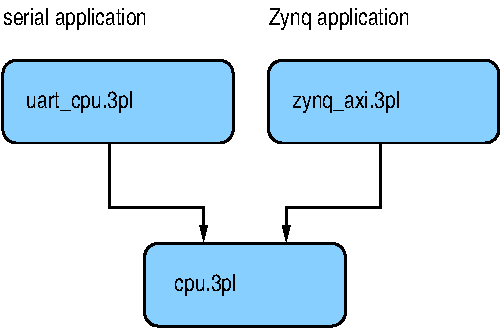
\includegraphics{cpu}

    
    xilinx/zynq\_axi.3pl is included in -\\
    boards/avnet/microzed\_7010.3pl\\
    boards/avnet/microzed\_7020.3pl\\
    boards/digilent/zybo.3pl
    
    xilinx/uart\_cpu.3pl is included in -\\
    boards/avnet/aes\_sp3a\_eval400.3pl\\
    board/gadget\_factory/papilio\_one\_100.3pl\\
    board/gadget\_factory/papilio\_one\_250.3pl\\
    board/gadget\_factory/papilio\_one\_500.3pl\\
    board/gadget\_factory/papilio\_pro\_lx4.3pl\\
    board/gadget\_factory/papilio\_pro\_lx9.3pl
    
    The class for the FPGA interface is created by -
    
    \begin{lstlisting}[gobble=4, language=threepl]
    class(cpu, CPU_API());
    \end{lstlisting}

    cpu.3pl -
    \blist   
    \item   defines class {\bf busCommon} which is used to describe each
            interface.    
    \item   creates an instance of class {\bf CPU\_CODEGEN} whose procedures
            create the logic to implement each type of interface.        
    \item   creates an instance of class {\bf CPU\_API} whose modules
            provide the application program interface. Procedures within
            this class create instances of {\bf busCommon} and add them to
            an interface list. {\bf busCommon} contains all the information
            necessary to create a CPU interface. Class {\bf CPU\_API} in
            turn assigns module create\_bus\_interfaces() as a trailer
            module.
    \blend
    
    Module create\_bus\_interfaces() executes at the end of immediate execution
    (it is a trailer module). It creates the basic CPU interface logic by
    calling module {\bf cpu\_interface} and then traverses the interface list
    and creates code for each interface via procedures in class {\bf
    CPU\_CODEGEN}.
    
    {\bf CPU\_API}, {\bf CPU\_CODEGEN}, {\bf create\_bus\_interfaces} and
    {\bf cpu\_interface} are defined in both UART\_CPU.3pl and zynq\_axi.3pl,
    as the underlying interface logic is quite different for the two platforms.






    \subsection{class library modules}
            
                
        \subsubsection{CPU\_API.signal\_interrupt - interrupt from a signal}\label{sec:lpcpusigint}

            {\bf Library: xilinx/cpu.3pl}

            {\bf Prototype:} \\
            \vsp
            \begin{lstlisting}[gobble=12, language=threepl]

                module
                signal_interrupt (str(event), value(sig, "log")) {}
            \end{lstlisting}

            {\bf Output parameters:} \\
            
            none.

            {\bf Input parameters:} \\
            {\bf event} is the event identifier string.\\
            {\bf sig} is the signal causing the event.\\
        
            {\bf In-line target execution:} \\
            no

            {\bf description:} \\
            This procedure generates a module which will cause a CPU interrupt
            when its input signal {\bf sig} is asserted.
            The argument to parameter {\bf event} is an identifier with
            which to refer to the interrupt in the CPU interface software.

            See also class procedure {\bf interrupt()}
            \autorefph{sec:lpcpuint} which generates a CPU interrupt when
            executed in the FPGA.
    
     
     
     
     
        \subsubsection{CPU\_API.dma\_read - DMA transfer to FPGA from CPU}\label{sec:lpcpudmar}

            {\bf Library: xilinx/cpu.3pl}

            {\bf Prototype:} \\
            \vsp
            \begin{lstlisting}[gobble=12, language=threepl]
                module
                dma_read (
                    queue(data, "bits:64")      // read data
                    <-
                    queue(address, "uint:32"),  // memory address
                    queue(burstlen, "uint:4"),  // burst length - 1
                    int(bus)                    // HP bus 0 to 3
                ) {}
            \end{lstlisting}

            {\bf Output parameters:} \\
            
            {\bf data} is the queue to which data from the transfer is returned.\\

            {\bf Input parameters:} \\
            {\bf address} is a queue supplying the CPU memory physical read address.\\
            {\bf burstlen} is a queue giving the burst length in the case of Zynq.\\
            {\bf bus} is the HP bus, 0 to 3, in the case of Zynq.\\
        
            {\bf In-line target execution:} \\
            no

            {\bf description:} \\
            This procedure generates a module which reads data from the CPU
            memory. For platforms with serial communications between the
            FPGA and the CPU this is not really DMA but instead data is transferred
            from CPU memory by a software thread.
            
            In the case of a platform with a serial interface only one input
            argument, {\bf address}, is valid - {\bf burstlen} and {\bf bus} must
            not be given arguments. \bf{This address is relative to a base address
            set by calling} {\bf set\_dma\_address()} \autorefph{tools_c_serial}.
            
            When an address becomes available on the {\bf address} input queue
            and the output {\bf data} queue is not full a DMA transfer (read)
            will take place. For a serial interface platform this is not a real
            DMA transfer but is carried out in software by a separate CPU
            thread.

            For the Zynq the address is a physical address. When an address and
            a burstlength become available on the {\bf address} and {\bf
            burstlen} input queues and the output {\bf data} queue is not full,
            a DMA transfer (read) will take place. The HP bus selected cannot be
            used for any other interfaces.

            See also class module {\bf CPU\_API.dma\_write()}
            \autorefph{sec:lpcpudmaw} which generates a DMA write module.



        \subsubsection{CPU\_API.dma\_write - DMA transfer from FPGA to CPU}\label{sec:lpcpudmaw}

            {\bf Library: xilinx/cpu.3pl}

            {\bf Prototype:} \\
            \vsp
            \begin{lstlisting}[gobble=12, language=threepl]
                module
                dma_write (
                    queue(data, "bits:64"),     // write data
                    queue(address, "uint:32"),  // memory address
                    queue(burstlen, "uint:4"),  // burst length - 1
                    int(bus)                    // HP bus 0 to 3
                ) {}
            \end{lstlisting}

            {\bf Output parameters:} \\
            
            None.

            {\bf Input parameters:} \\
            {\bf data} is a queue supplying data for the transfer.\\
            {\bf address} is a queue supplying the CPU memory physical write address.\\
            {\bf burstlen} is a queue giving the burst length in the case of Zynq.\\
            {\bf bus} is the HP bus, 0 to 3, in the case of Zynq.\\
        
            {\bf In-line target execution:} \\
            no

            {\bf description:} \\
            This procedure generates a module which writes data to the CPU
            memory. For platforms with serial communications between the
            FPGA and the CPU this is not really DMA but instead data is transferred
            to CPU memory by a software thread.
            
            In the case of a platform with a serial interface only two input
            arguments, {\bf data} and {\bf address}, are valid - {\bf burstlen}
            and {\bf bus} must not be given arguments. \bf{This address is
            relative to a base address set by calling} {\bf set\_dma\_address()}
            \autorefph{tools_c_serial}.
            
            When data and an address become available on the {\bf data} and {\bf
            address} input queues a DMA transfer (read) will take place. For a
            serial interface platform this is not a real DMA transfer but is
            carried out in software by a separate CPU thread.

            For the Zynq When data, an address and a burstlength become available
            on the {\bf data}, {\bf address} and {\bf burstlen} input queues a
            DMA transfer (write) will take place. The HP bus selected cannot be
            used for any other interfaces.

            See also class module {\bf CPU\_API.dma\_read()}
            \autorefph{sec:lpcpudmar} which generates a DMA read module.



    
    \subsection{class library procedures}
            
                
        \subsubsection{CPU\_API.interrupt - interrupt procedure}\label{sec:lpcpuint}

            {\bf Library: xilinx/cpu.3pl}

            {\bf Prototype:} \\
            \vsp
            \begin{lstlisting}[gobble=12, language=threepl]

                procedure
                interrupt (str(event)) {}
            \end{lstlisting}

            {\bf Output parameters:} \\
            
            none.

            {\bf Input parameters:} \\
            {\bf event} is the event identifier string.\\
        
            {\bf In-line target execution:} \\
            yes

            {\bf description:} \\
            This procedure generates an interrupt when executed in the FPGA.
            The argument to parameter {\bf event} is an identifier with
            which to refer to the interrupt in the CPU interface software.

            See also class module {\bf signal\_interrupt()}
            \autorefph{sec:lpcpusigint} which creates a module which sources an
            interrupt from a signal.





        \subsubsection{CPU\_API.read - a CPU-readable interface}\label{sec:lpcpuread}

            {\bf Library: xilinx/cpu.3pl}

            {\bf Prototype:} \\
            \vsp
            \begin{lstlisting}[gobble=12, language=threepl]
                procedure
                read (
                        static(access, "log"),
                        varargs
                        <- 
                        str(name),
                        var(in),
                        varargs
                    ) {}
            \end{lstlisting}

            {\bf Output parameters:} \\
            {\bf access} is an optional static logical variable which is true
            for one clock cycle following a CPU read.
            {\bf varargs} optional output, parameters {\bf out} and {\bf count}.\\

            {\bf Input parameters:} \\
            {\bf in} is the value, queue, cmemory or rmemory mode variable
            to be read.\\
            {\bf name} is a string identifier for the interface.\\
            {\bf varargs} optional input parameters {\bf wordcount}, {\bf ilevel} and
                {\bf port}.\\
        
            {\bf In-line target execution:} \\
            no

            {\bf description:} \\
            This procedure creates a module which provides a CPU-readable
            interface for the the CPU for  3PL variables of mode value, static,
            queue, cmemory or rmemory.
            
            In the case of Zynq the interface uses AXI bus GP0.            
            The size of the input data type must not exceed 256 bits as the CPU
            interface software limits burst transfers to 8 32-bit words.
            
            Boards having a serial interface to the CPU use that interface.
            The size of the input data type must not exceed 1016 bits (127 bytes).
            
            The module is created at the end of immediate execution from
            arguments queued by this procedure. It can be any type, primitive or
            compound.
                        
            It is a common wrapper for the procedures \\
            {\bf CPU\_API.read\_value()} \autorefph{sec:lpcpurdvalue} \\
            {\bf CPU\_API.read\_queue()} \autorefph{sec:lpcpurdqueue} \\
            {\bf CPU\_API.read\_memory()} \autorefph{sec:lpcpurdmem} \\
            
            Parameter {\bf name} is a string identifier that can be used
            in the CPU code to refer to this interface.
            
            Parameter {\bf in} is the input variable or expression to be read
            by the CPU.
           
            Optional input and output varargs parameters are -
            
            \begin{tabular}{| l | l | l |}
            \hline
                    & input varargs         & output varargs    \\
            \hline \hline
            value   &                       &                   \\
            static  &                       &                   \\
            \hline
            queue   &   wordcount ilevel    & out count         \\
            \hline
            cmemory & port                  &                   \\
            rmemory &                       &                   \\
            \hline
            \end{tabular}




            
            \vspace{\baselineskip}\vspace{\baselineskip}
            {\Large \bfseries Value or Static mode}

                
                            Parameter {\bf in} is the value-mode input variable or expression.
            Since it is value mode the argument may be a value mode variable,
            static mode variable or an expression containing these. An expression
            must not contain a queue read.            
            
            The module is created at the end of immediate execution from arguments
            queued by this procedure. It can be any type, primitive or compound. The
            optional output static logical variable {\bf access} goes true for one
            clock cycle to indicate that a read has occurred.
            
            This procedure can be called via the more cryptic and general
            procedure {\bf cpu\_api.read()} \autorefph{sec:lpcpuread} instead.
            
            In the case of Zynq the interface uses AXI bus GP0.            
            The size of the input data type must not exceed 256 bits as the CPU
            interface software limits burst transfers to 8 32-bit words.
            
            Boards having a serial interface to the CPU use that interface.
            The size of the input data type must not exceed 1016 bits (127 bytes).
            

            The optional output static logical variable {\bf access} goes true
            for one clock cycle to indicate that a read has occurred.
            
            The clock domain of output {\bf access} need not be the same as
            that of {\bf in}. If {\bf access} has no clock domain it will be
            given the bus clock domain.
            
            The parameters associated with this bus interface, including an
            allocated bus address, are written
            to the {\em design}.info file.

            The utility info2c is used to process this file and create
            an include file {\em design}.h which contains a funcion
            definition to access this interface. for example the 3PL
            code
            \begin{lstlisting}[gobble=12, language=threepl]
               cpu_read_value("alpha", v);
            \end{lstlisting}
            will result in info2c producing a declaration like
            \begin{lstlisting}[gobble=12, language=C]
               uint32_t alpha_read (fpga_t * fpga) {}
            \end{lstlisting}
            
            When the CPU reads a value it is sampling that value, hence data may
            be lost if the sampling rate is lower than the rate at which data
            changes. The data sampling logic ensures that the data is a valid
            sample even when the source is changing at the time of the
            read. This is a primitive interface which depends on additional
            protocols being imposed by the application code. For example to
            guarantee data integrity a write to register the data in a static
            variable prior to reading could be used. For a more complex interface see {\bf cpu\_api.read\_queue()}
            \autorefph{sec:lpcpurdqueue}.
            
            On running info2c on the .json file the following C function will have been
            defined for interface {\em name} -
            
            \begin{tabular}{| l | l |}
            \hline
            function                   &                 \\ \hline \hline
            fpga\_{\em name}\_read()   & read a datum    \\ \hline
            \end{tabular}
            
            Example: \\
            If 3PL source file prog.3pl contains the following \\
            \begin{lstlisting}[gobble=12, language=threepl]
               class(cpu, cpu_api());
               
               static(s, "uint:16");
               .
               .
               cpu.read_value("S1", s);
               .
               .
            \end{lstlisting}
            the CPU code should contain something like \\
            \begin{lstlisting}[gobble=12, language=C]
                   #include "prog_fpga.h"
                   .
                   .
                   fpga_t *fpga = NULL;
                   int     d;
                   .
                   .
                   fpga_open(portName);
                   .
                   .
                   d = fpga_S1_read(fpga);
                   .
            \end{lstlisting}
            
            This procedure creates no in-line target code so the current clock domain
            when this procedure is called is not relevant. The clock domain is not
            changed by this procedure,
            The CPU code in Python3 should contain something like \\
            \begin{lstlisting}[gobble=12, language=python]
                import sys
                sys.path.append("/Users/......./install/3pl")
                import info2py
                import prog_fpga as fpga

                fpga_open()

                fpga = info2py.info_from_file("prog")   # load info from prog.info file

                d = fpga.P1_read()

            \end{lstlisting}

                        


            \vspace{\baselineskip}\vspace{\baselineskip}
            {\Large \bfseries Queue mode}
                        


                            Parameter {\bf in} is the queue-mode input variable.
            
            The queue must be written somewhere in the program (queues without
            sources result in a fatal error on completion of immediate
            execution). When the module is created the argument queue must have
            an established write clock domain or a fatal error is generated.

            If the input queue is read anywhere else in the program (i.e. other
            than in this module) then it must be read in the bus clock domain
            since that is the clock domain in which it is read in the module
            created by this procedure.

            If optional parameter {\bf wordcount} has an argument and it
            is true, the number of words in the queue buffer can be interrogated
            by the CPU. The input queue may have any of the allowed buffer sizes.
            If the queue is asynchronous, i.e. the read domain is not the bus
            clock domain, the count will not be exact but will be a guaranteed
            minimum number of readable data.

            If optional parameter {\bf wordcount} has an argument and it
            is false, the data returned from reading the number of words in the
            buffer is 0 or 1 instead of a count. A return of 1 means the queue
            buffer is not empty, i.e. can be read. This option is provided to
            simplify the logic where a simple empty/non-empty status is required.

            If optional parameter {\bf wordcount} has no argument then
            there will no interface to directly read the number of words in the
            queue buffer, however an interrupt may be used instead.            

            Note that an empty queue is guaranteed to return all ones to the CPU
            when read. For most data types this single value will usually be
            invalid and hence in that case it can be used as an indication of an
            empty queue. This can be used instead of explicitly reading the
            available word count.

            If an argument to optional parameter {\bf ilevel} is provided then a
            level interrupt on queue buffer status is established as follows -

            If there is no argument then no interrupt is provided.

            If the argument is type "log" with value false then the interrupt will
            be asserted when the queue buffer is not empty.

            If the argument is type "log" with value true then the interrupt will be
            asserted when the number of words in the buffer equals or exceeds a
            level which has been written to the interface from the CPU. The initial
            value of this level is 1. A level value of 0 should not be written to
            the interface as that will result in a continuous level interrupt
            regardless of queue state.

            If the argument is type "uint" or "int" then the interrupt will be
            asserted when the number of words in the buffer equals or exceeds the
            fixed value specified by the integer argument.

            The optional output parameter {\bf count} provides a count of the
            number of data in the queue. The inbuilt function queuewords() can
            only be used in a module which reads the queue, which is usually not
            the case where {\bf cpu\_api.read\_queue()} is the queue destination.
            {\bf count} must have clock domain {\bf bus\_clk}. If it has no clock
            domain, {\bf cpu\_api.read\_queue()} will set it to {\bf bus\_clk}.
            The width of {\bf count} must be sufficient to hold the input queue
            depth.

            If optional output parameter {\bf out} has an argument, each datum
            read from the input queue {\bf in} to the CPU local bus is also
            written to queue {\bf out}. The type of {\bf out} must be such that
            it can be assigned from {\bf in}. {\bf out} should not be allowed to
            block since it cannot stop data being popped from {\bf in} to the CPU
            bus. While {\bf out} in unavailable for writing, no attempt is made
            to write data popped from {\bf in} to it.

            If optional output parameter {\bf access} has an argument, the static
            variable of type "log" is assigned true for one clock cycle every
            time a datum is popped from the input queue {\bf in}. {\bf access}
            may have any clock domain.
            
            On running info2c on the .json file the following C functions will have
            been defined for interface {\em name} -
            
            \begin{tabular}{| l | l | l |}
            \hline
            function                                 & action when?           &                         \\ \hline \hline
            fpga\_{\em name}\_read()                 & always                 & read a datum            \\ \hline
            fpga\_{\em name}\_avail\_read()          & wordcount has argument & read number of words    \\ \hline
            fpga\_{\em name}\_avail\_thresh\_write() & ilevel "log" true      & set interrupt threshold \\ \hline
            fpga\_{\em name}\_enable()               & ilevel has argument    & enable interrupt        \\ \hline
            fpga\_{\em name}\_disable()              & ilevel has argument    & disable interrupt       \\ \hline 
            fpga\_{\em name}\_wait()                 & ilevel has argument    & wait on interrupt       \\ \hline  
            \end{tabular}
            
            Example: \\
            If 3PL source file prog.3pl contains the following \\
            \begin{lstlisting}[gobble=12, language=threepl]
                class(cpu, cpu_api());
                
                queue(p, "uint:16");
                .
                .
                cpu.read("P1", p, wordcount=false, ilevel=false);
                .
                .
            \end{lstlisting}
            the CPU code in C should contain something like \\
            \begin{lstlisting}[gobble=12, language=C]
                #include "prog_fpga.h"
                .
                .
                fpga_t *fpga = NULL;
                int     d[...];
                int     i = 0;
                .
                .
                fpga_open();
                .
                .
                fpga_P1_event_wait(fpga);
                while (fpga_P1_avail_read(fpga) != 0)
                    d[i++] = fpga_P1_read(fpga);
                .
            \end{lstlisting}
            The code will wait until the queue p goes from empty to non-empty
            when an interrupt will release the wait. A loop while the queue
            remains non-empty reads until the queue is empty. Note that since
            {\bf wordcount} is given an argument but the value is false, the count
            will only have values 0/1 for empty/not-empty.
           
            This procedure creates no in-line target code so the current clock
            domain when this procedure is called is not relevant. The clock domain
            is not changed by this procedure,
            
            The CPU code in Python3 should contain something like \\
            \begin{lstlisting}[gobble=12, language=python]
                import sys
                sys.path.append("/Users/......./install/3pl")
                import info2py
                from cpu_serial import *

                fpga_open()

                fpga = info2py.info_from_file("prog")   # load info from prog.info file

                d = []
                fpga.P1_wait()
                while (fpga.P1_avail_read() != 0)
                    d.append = fpga.P1_read()

            \end{lstlisting}
            
            Note that in the unusual case where a queue variable is both read and
            written by the CPU and is not otherwise accessed in the FPGA the input
            and output clock domains of the queue will be undefined. To overcome
            this the clock domain can be set when the queu is created, e.g.
            
            \begin{lstlisting}[gobble=12, language=threepl]
            queue(q, "uint10", domain=null);
            \end{lstlisting}
            
            which will set both the input (write) and output (read) clock domains
            to the current clock domain - see \autorefph{sec:ipqueue}).

                        


            
            \vspace{\baselineskip}\vspace{\baselineskip}
            {\Large \bfseries cmemory or rmemory mode}
            
                        
                            Parameter {\bf in} is the cmemory-mode or rmemory-mode input variable.
            
            If optional output parameter {\bf access} has an argument, the
            static variable of type "log" is assigned true for one clock cycle
            every time the port of {\bf in} is read. {\bf access} may have any
            clock domain.
            
            In the case of Zynq the interface uses AXI bus GP0.            
            The size of the input data type must not exceed 256 bits as the CPU
            interface software limits burst transfers to 8 32-bit words.
            
            Boards having a serial interface to the CPU use that interface.
            The size of the input data type must not exceed 1016 bits (127 bytes).
            
            This interface can use any memory port and that port can also be
            used by other application code, but no arbitration of shared access
            via a port is provided. Coincident access will usually result in
            data corruption. If it is not feasible to dedicate a port to CPU
            access then the CPU application code must limit acccess to the
            memory to times when it is known that the FPGA logic will not also
            be accessing the memory port.
            
            On running info2c on the .json file the following C function will have been
            defined for interface {\em name} -
            
            \begin{tabular}{| l | l |}
            \hline
            function                 &                                \\ \hline \hline
            fpga\_{\em name}\_read() & read a datum from FPGA memory  \\ \hline
            \end{tabular}
            
            Example: \\
            If 3PL source file prog.3pl contains the following \\
            \begin{lstlisting}[gobble=12, language=threepl]
               class(cpu, cpu_api());
               rmemory(m, 2, "uint:8", "uint:16");
               .
               .
               cpu.read_memory("MEM1", m, 0);
               .
               .
            \end{lstlisting}
            then for zynq the CPU code should contain something like \\
            \begin{lstlisting}[gobble=12, language=C]
                   #include "prog.h"
                   .
                   .
                   fpga_t *fpga = NULL;
                   int     d;
                   .
                   .
                   fpga_open();
                   .
                   .
                   d = fpga_MEM1_read(addr);
                   .
            \end{lstlisting}
            where addr is the memory address. The returned data is assigned
            to variable {\bf d}.

            This procedure creates no in-line target code so the current clock domain
            when this procedure is called is not relevant. The clock domain is not
            changed by this procedure,

            








        \subsubsection{CPU\_API.write - a CPU-writable interface}\label{sec:lpcpuwrite}

            {\bf Library: xilinx/cpu.3pl}

            {\bf Prototype:} \\
            \vsp
            \begin{lstlisting}[gobble=12, language=threepl]
                procedure
                write (
                        var(out),
                        varargs
                        <- 
                        str(name),
                        varargs
                    ) {
            \end{lstlisting}

            {\bf Output parameters:} \\
            {\bf out} is the target variable to be written to \\
            {\bf varargs} optional output parameter {\bf access} \\

            {\bf Input parameters:} \\
            {\bf name} is a string identifier for the interface.\\
            {\bf varargs} optional input parameters {\bf freecount}, {\bf ilevel}, {\bf port}
            and {\bf reset}.\\
        
            {\bf In-line target execution:} \\
            no

            {\bf description:} \\
            This procedure provides a write interface for the the CPU for 
            3PL variables of mode static, queue, cmemory or rmemory.
            
            In the case of Zynq the interface uses AXI bus GP0.            
            The size of the input data type must not exceed 256 bits as the CPU
            interface software limits burst transfers to 8 32-bit words.
            
            Boards having a serial interface to the CPU use that interface.
            The size of the input data type must not exceed 1016 bits (127 bytes).
            
            The module is created at the end of immediate execution from
            arguments queued by this procedure. It can be any type, primitive or
            compound.
                        
            It is a common wrapper for the procedures \\
            {\bf CPU\_API.write\_static()} \autorefph{sec:lpcpuwrstat} \\
            {\bf CPU\_API.write\_queue()} \autorefph{sec:lpcpuwrqueue} \\
            {\bf CPU\_API.write\_memory()} \autorefph{sec:lpcpuwrmem} \\
            
            Parameter {\bf name} is a string identifier that can be used
            in the CPU code to refer to this interface.
            
            Parameter {\bf out} is the output variable to be written to
            by the CPU.

            The only optional output parameter is {\bf access} which must have
            a static mode argument of type "log". If this optional parameter is
            given an argument then parameter {\bf out} may be omitted. In that
            case the write serves only to generate a single cycle pulse to
            the {\bf access} argument in the FPGA.
           
            Optional input varargs parameters are -
            
            \begin{tabular}{| l | l |}
            \hline
                    & input varargs             \\
            \hline \hline
            static  &                           \\
            \hline
            queue   & freecount ilevel reset    \\
            \hline
            cmemory & port                      \\
            rmemory &                           \\
            \hline
            \end{tabular}





            
            \vspace{\baselineskip}\vspace{\baselineskip}
            {\Large \bfseries Static mode}

                        
                            Parameter {\bf out} is the static-mode output variable. Its argument
            may be omitted if the optional parameter {\bf access} is given an argument.
            
            In the case of Zynq the interface uses AXI bus GP0.            
            The size of the output data type must not exceed 256 bits as the CPU
            interface software limits burst transfers to 8 32-bit words.
            
            Boards having a serial interface to the CPU use that interface.
            The size of the output data type is not limited.

            Output parameter {\bf out} is examined in order to determine its clock
            domain. If it has no clock domain it is given the bus clock domain.

            On running info2c on the .json file the following C function will
            have been defined for interface {\em name} -
            
            \begin{tabular}{| l | l |}
            \hline
            function                   & action         \\ \hline \hline
            fpga\_{\em name}\_write()  & write a datum  \\ \hline
            \end{tabular}
            
            Example: \\
            If 3PL source file prog.3pl contains the following \\
            \begin{lstlisting}[gobble=12, language=threepl]
               class(cpu, cpu_api());
               
               static(s, "uint:16");
               .
               .
               cpu.write_static(s <- "S2");
               .
               .
            \end{lstlisting}
            then for zynq the CPU code should contain something like \\
            \begin{lstlisting}[gobble=12, language=C]
                   #include "prog_fpga.h"
                   .
                   .
                   int     d;
                   .
                   .
                   fpga_open();
                   .
                   .
                   fpga_S2_write(d);          // write
                   .
            \end{lstlisting}

            This procedure creates no in-line target code so the current clock domain
            when this procedure is called is not relevant. The clock domain is not
            changed by this procedure,


                        
            

            \vspace{\baselineskip}\vspace{\baselineskip}
            {\Large \bfseries Queue mode}
                        


                            In the case of Zynq the interface uses AXI bus GP0.            
            The size of the output data type must not exceed 256 bits as the CPU
            interface software limits burst transfers to 8 32-bit words.
            
            Boards having a serial interface to the CPU use that interface.
            The size of the output data type is not limited.

            The queue must be read somewhere in the program (queues without
            sinks result in a fatal error on completion of immediate execution).
            When the module is created the argument queue must have an established
            read clock domain or a fatal error is generated.

            If the output queue is written anywhere else in the program (i.e. other
            than in this module) then it must be written in the bus clock domain
            (c100) since that is the clock domain in which it is written in this
            module.

            If the argument to {\bf freecount} is true the number of free entries in
            the queue buffer can be interrogated by the CPU. The output queue may
            have any of the allowed buffer sizes. If the queue is asynchronous, i.e.
            the write domain is not the bus clock domain (c100), the count will not
            be exact but will be a guaranteed minimum number of writable spaces.

            If the argument to {\bf freecount} is false the data returned from
            reading the number of free spaces in the buffer is 0 or 1 instead of a
            count. A return of 1 means the queue buffer is not full, i.e. can be
            written. This option is provided to simplify the logic where a simple
            full/non-full status is required.

            If {\bf freecount} has no argument then there will no interface to
            directly read the space remaining in the queue buffer, however an
            interrupt may be used instead.            

            Arguments to parameter {\bf ilevel} control provision of a level
            interrupt on queue buffer status as follows -

            If there is no argument then no interrupt is provided.

            If the argument is type "log" with value false then the interrupt will
            be asserted when the queue buffer is not full.

            If the argument is type "log" with value true then the interrupt will be
            asserted when the number of free spaces in the buffer equals or exceeds
            a level which has been written to the interface from the CPU. The
            initial value of this level is 1. A level value of 0 should not be
            written to the interface as that will result in a continuous level
            interrupt regardless of queue state.

            If the argument is type "uint" or "int" then the interrupt will be
            asserted when the number of free spaces in the buffer equals or exceeds
            the fixed value specified by the integer argument. Again this should not
            be 0.

            If parameter {\bf reset} has an argument it provides a means of
            resetting (clearing) the output queue. The argument may have a
            different clock domain to that of the write side of the queue and hence
            this may be more convenient than directly resetting the queue where a
            change of clock domain may need to be explicitly provided.

            Note that a write to a queue variable from {\bf cpu\_api.write\_queue()} (or
            indeed from anywhere) can be detected within the FPGA by means of the
            inbuilt function {\bf waswritten()} \autorefph{sec:ifwaswritten}. When
            using this function the clock domain must be the same as that of the
            queue write, i.e. {\bf bus\_clk}.
            Parameter {\bf out} is the queue-mode output variable.
            
            On running info2c on the .json file the following C functions will have
            been defined for interface {\em name} -
            
            \begin{tabular}{| l | l | l |}
            \hline
            function                                 & when                   &                            \\ \hline \hline
            fpga\_{\em name}\_write()                & always                 & write a datum              \\ \hline
            fpga\_{\em name}\_avail\_read()          & freecount has argument & read number of spaces free \\ \hline
            fpga\_{\em name}\_avail\_thresh\_write() & ilevel "log" true      & set interrupt threshold    \\ \hline
            fpga\_{\em name}\_enable()               & ilevel has argument    & enable interrupt           \\ \hline
            fpga\_{\em name}\_disable()              & ilevel has argument    & disable interrupt          \\ \hline 
            fpga\_{\em name}\_wait()                 & ilevel has argument    & wait on interrupt          \\ \hline  
            \end{tabular}


            
            Example: \\
            If 3PL source file prog.3pl contains the following \\
            \begin{lstlisting}[gobble=12, language=threepl]
               class(cpu, cpu_api());
               queue(p, "uint:16");
               .
               .
               cpu.write_queue(p <- "P2",, true);
               .
               .
            \end{lstlisting}
            then for zynq the CPU code should contain something like \\
            \begin{lstlisting}[gobble=12, language=C]
                   #include "prog_fpga.h"
                   .
                   .
                   fpga_t *fpga = NULL;
                   int     d[...];
                   int     i = 0;
                   int     n = sizeof(d) / sizeof int;
                   .
                   .
                   fpga_open(portName, INTERRUPTS);
                   .
                   .
                   fpga_P2_avail_thresh_write(fpga, n); // set interrupt level
                   fpga_P2_wait(fpga);                  // wait for interrupt
                   for (i=0 ; i<n ; i++) {              // transmit data block
                       fpga_P2_write(fpga, d[i]);       // write item
                   fpga_P2_enable(fpga);                // enable interrupt
                   .
            \end{lstlisting}
            
            or perhaps -
            \begin{lstlisting}[gobble=12, language=threepl]
               class(cpu, cpu_api());
               queue(p, "uint:16");
               .
               .
               cpu.write_queue(p <- "P2", false);
               .
               .
            \end{lstlisting}
            then for zynq the CPU code should contain something like \\
            \begin{lstlisting}[gobble=12, language=C]
                   #include "prog_fpga.h"
                   .
                   .
                   fpga_t *fpga = NULL;
                   int     d[...];
                   int     i = 0;
                   int     n = sizeof(d) / sizeof int;
                   .
                   .
                   fpga_open(portName, INTERRUPTS);
                   .
                   .
                   for ( i=0 ; i<n ; i++) {                // transmit data block
                       while (fpga_P2_avail(fpga) == 0)    // poll until not full
                           ;
                       fpga_P2_write(fpga, d[i]);          // write item
                   }
                   .
            \end{lstlisting}

            This procedure creates no in-line target code so the current clock domain
            when this procedure is called is not relevant. The clock domain is not
            changed by this procedure,
            
            {\bf The support CPU software for the UART CPU interface is still
            under development, but application code wil be similar to the
            above.}

                        
            

            
            \vspace{\baselineskip}\vspace{\baselineskip}
            {\Large \bfseries cmemory or rmemory mode}
            
                            Parameter {\bf out} is the cmemory or rmemory mode output variable.

            
            In the case of Zynq the interface uses AXI bus GP0.            
            The size of the output data type must not exceed 256 bits as the CPU
            interface software limits burst transfers to 8 32-bit words.
            
            Boards having a serial interface to the CPU use that interface.
            The size of the output data type is not limited.
            
            This interface can use any memory port and that port can also be
            used by other application code, but no arbitration of shared access
            via a port is provided. Coincident access will usually result in
            data corruption. If it is not feasible to dedicate a port to CPU
            access then the CPU application code must limit acccess to the
            memory to times when it is known that the FPGA logic will not also
            be accessing the memory port.
            
            On running info2c on the .json file the following C function will have been
            defined for interface {\em name} -
            
            \begin{tabular}{| l | l |}
            \hline
            function                   &                              \\ \hline \hline
            fpga\_{\em name}\_write()  & write a datum to FPGA memory \\ \hline
            \end{tabular}
            
            Example: \\
            If 3PL source file prog.3pl contains the following \\
            \begin{lstlisting}[gobble=12, language=threepl]
               class(cpu, cpu_api())
               rmemory(m, 2, "uint:8", "uint:16");
               .
               .
               cpu.write_memory(m <- "MEM2", 1);
               .
               .
            \end{lstlisting}
            then for zynq the CPU code should contain something like \\
            \begin{lstlisting}[gobble=12, language=C]
                   #include "prog.h"
                   .
                   .
                   fpga_t *fpga = NULL;
                   int     d;
                   .
                   .
                   fpga_open(portName, INTERRUPTS);
                   .
                   .
                   fpga_MEM2_write(fpga, addr, d);
                   .
            \end{lstlisting}
            where addr is the memory addressd the data to be written.

            This procedure creates no in-line target code so the current clock domain
            when this procedure is called is not relevant. The clock domain is not
            changed by this procedure,







        \subsubsection{CPU\_API.read\_memory - a CPU-readable interface
                                            to a memory}\label{sec:lpcpurdmem}

            {\bf Library: xilinx/cpu.3pl}

            {\bf Prototype:} \\
            \vsp
            \begin{lstlisting}[gobble=12, language=threepl]
               global procedure
               cpu_api.read_memory (
                   static(access, "log")
                   <-
                   str(name),
                   var(mem),
                   int(port)
               ) {}
            \end{lstlisting}

            {\bf Output parameters:} \\
            {\bf access} is an optional access indicator.\\        

            {\bf Input parameters:} \\
            {\bf name} is a string identifier for the interface.\\
            {\bf mem} is the cmemory or rmemory variable.\\
            {\bf port} is memory port, 0 or 1, to be used for the read.
        
            {\bf In-line target execution:} \\
            no

            {\bf description:} \\
            This procedure creates a module which allows the CPU to read
            from a registered output memory (rmemory) or a CLB memory (cmemory)
            via the GP1 AXI bus.
            
            This procedure can be called via the more cryptic and general
            procedure {\bf CPU\_API.read()} \autorefph{sec:lpcpuread} instead.

                        Parameter {\bf in} is the cmemory-mode or rmemory-mode input variable.
            
            If optional output parameter {\bf access} has an argument, the
            static variable of type "log" is assigned true for one clock cycle
            every time the port of {\bf in} is read. {\bf access} may have any
            clock domain.
            
            In the case of Zynq the interface uses AXI bus GP0.            
            The size of the input data type must not exceed 256 bits as the CPU
            interface software limits burst transfers to 8 32-bit words.
            
            Boards having a serial interface to the CPU use that interface.
            The size of the input data type must not exceed 1016 bits (127 bytes).
            
            This interface can use any memory port and that port can also be
            used by other application code, but no arbitration of shared access
            via a port is provided. Coincident access will usually result in
            data corruption. If it is not feasible to dedicate a port to CPU
            access then the CPU application code must limit acccess to the
            memory to times when it is known that the FPGA logic will not also
            be accessing the memory port.
            
            On running info2c on the .json file the following C function will have been
            defined for interface {\em name} -
            
            \begin{tabular}{| l | l |}
            \hline
            function                 &                                \\ \hline \hline
            fpga\_{\em name}\_read() & read a datum from FPGA memory  \\ \hline
            \end{tabular}
            
            Example: \\
            If 3PL source file prog.3pl contains the following \\
            \begin{lstlisting}[gobble=12, language=threepl]
               class(cpu, cpu_api());
               rmemory(m, 2, "uint:8", "uint:16");
               .
               .
               cpu.read_memory("MEM1", m, 0);
               .
               .
            \end{lstlisting}
            then for zynq the CPU code should contain something like \\
            \begin{lstlisting}[gobble=12, language=C]
                   #include "prog.h"
                   .
                   .
                   fpga_t *fpga = NULL;
                   int     d;
                   .
                   .
                   fpga_open();
                   .
                   .
                   d = fpga_MEM1_read(addr);
                   .
            \end{lstlisting}
            where addr is the memory address. The returned data is assigned
            to variable {\bf d}.

            This procedure creates no in-line target code so the current clock domain
            when this procedure is called is not relevant. The clock domain is not
            changed by this procedure,

            
            See also - \\
            {\bf CPU\_API.read()} \autorefph{sec:lpcpuread} \\
            {\bf CPU\_API.write()} \autorefph{sec:lpcpuwrite} \\
            {\bf CPU\_API.read\_value()} \autorefph{sec:lpcpurdvalue} \\
            {\bf CPU\_API.write\_static()} \autorefph{sec:lpcpuwrstat} \\
            {\bf CPU\_API.read\_queue()} \autorefph{sec:lpcpurdqueue} \\
            {\bf CPU\_API.write\_queue()} \autorefph{sec:lpcpuwrqueue} \\
            {\bf CPU\_API.write\_memory()} \autorefph{sec:lpcpuwrmem} \\
            {\bf CPU\_API.dma\_write()} \autorefph{sec:lmzynqwrdma} \\
            {\bf CPU\_API.dma\_read()} \autorefph{sec:lmzynqrddma} \\



            

            
                





        \subsubsection{CPU\_API.read\_queue - a CPU read from a queue
                                        variable}\label{sec:lpcpurdqueue}

            {\bf Library: xilinx/cpu.3pl}

            {\bf Prototype:} \\
            \vsp
            \begin{lstlisting}[gobble=12, language=threepl]
               global procedure
               cpu_api.read_queue (
                   static(access, "log"),
                   static(count),
                   queue(out)
                   <-
                   str(name),
                   queue(in),
                   log(wordcount),
                   var(ilevel)
               ) {}
            \end{lstlisting}

            {\bf Output parameters:} \\
            {\bf access} is an optional access indicator.\\        
            {\bf count} is an optional queue occupancy count.\\
            {\bf out} is an optional output queue.\\

            {\bf Input parameters:} \\            
            {\bf name} is a string identifier for the interface.\\
            {\bf in} is the input queue.\\            
            {\bf wordcount} is an optional flag to enable the number of words
            available in the queue to be determined.\\
            {\bf ilevel} is an optional argument to allow the queue buffer level
            at which an interrupt occurs to be set.\\
        
            {\bf In-line target execution:} \\
            no

            {\bf description:} \\
            This procedure creates a module which is an interface to allow the CPU
            to read a queue variable. The module is created at the end of immediate
            execution from arguments queued by this procedure. The queue can be any
            type, primitive or compound. When the CPU reads from the queue a datum
            is removed from the queue buffer. If the CPU reads from the specified
            address when the queue is empty the read will return all ones .
            
            This procedure can be called via the more cryptic and general
            procedure {\bf CPU\_API.read()} \autorefph{sec:lpcpuread} instead.
            
            In the case of Zynq the interface uses AXI bus GP0.            
            The size of the input data type must not exceed 256 bits as the CPU
            interface software limits burst transfers to 8 32-bit words.
            
            Boards having a serial interface to the CPU use that interface.
            The size of the input data type must not exceed 1016 bits (127 bytes).

                        Parameter {\bf in} is the queue-mode input variable.
            
            The queue must be written somewhere in the program (queues without
            sources result in a fatal error on completion of immediate
            execution). When the module is created the argument queue must have
            an established write clock domain or a fatal error is generated.

            If the input queue is read anywhere else in the program (i.e. other
            than in this module) then it must be read in the bus clock domain
            since that is the clock domain in which it is read in the module
            created by this procedure.

            If optional parameter {\bf wordcount} has an argument and it
            is true, the number of words in the queue buffer can be interrogated
            by the CPU. The input queue may have any of the allowed buffer sizes.
            If the queue is asynchronous, i.e. the read domain is not the bus
            clock domain, the count will not be exact but will be a guaranteed
            minimum number of readable data.

            If optional parameter {\bf wordcount} has an argument and it
            is false, the data returned from reading the number of words in the
            buffer is 0 or 1 instead of a count. A return of 1 means the queue
            buffer is not empty, i.e. can be read. This option is provided to
            simplify the logic where a simple empty/non-empty status is required.

            If optional parameter {\bf wordcount} has no argument then
            there will no interface to directly read the number of words in the
            queue buffer, however an interrupt may be used instead.            

            Note that an empty queue is guaranteed to return all ones to the CPU
            when read. For most data types this single value will usually be
            invalid and hence in that case it can be used as an indication of an
            empty queue. This can be used instead of explicitly reading the
            available word count.

            If an argument to optional parameter {\bf ilevel} is provided then a
            level interrupt on queue buffer status is established as follows -

            If there is no argument then no interrupt is provided.

            If the argument is type "log" with value false then the interrupt will
            be asserted when the queue buffer is not empty.

            If the argument is type "log" with value true then the interrupt will be
            asserted when the number of words in the buffer equals or exceeds a
            level which has been written to the interface from the CPU. The initial
            value of this level is 1. A level value of 0 should not be written to
            the interface as that will result in a continuous level interrupt
            regardless of queue state.

            If the argument is type "uint" or "int" then the interrupt will be
            asserted when the number of words in the buffer equals or exceeds the
            fixed value specified by the integer argument.

            The optional output parameter {\bf count} provides a count of the
            number of data in the queue. The inbuilt function queuewords() can
            only be used in a module which reads the queue, which is usually not
            the case where {\bf cpu\_api.read\_queue()} is the queue destination.
            {\bf count} must have clock domain {\bf bus\_clk}. If it has no clock
            domain, {\bf cpu\_api.read\_queue()} will set it to {\bf bus\_clk}.
            The width of {\bf count} must be sufficient to hold the input queue
            depth.

            If optional output parameter {\bf out} has an argument, each datum
            read from the input queue {\bf in} to the CPU local bus is also
            written to queue {\bf out}. The type of {\bf out} must be such that
            it can be assigned from {\bf in}. {\bf out} should not be allowed to
            block since it cannot stop data being popped from {\bf in} to the CPU
            bus. While {\bf out} in unavailable for writing, no attempt is made
            to write data popped from {\bf in} to it.

            If optional output parameter {\bf access} has an argument, the static
            variable of type "log" is assigned true for one clock cycle every
            time a datum is popped from the input queue {\bf in}. {\bf access}
            may have any clock domain.
            
            On running info2c on the .json file the following C functions will have
            been defined for interface {\em name} -
            
            \begin{tabular}{| l | l | l |}
            \hline
            function                                 & action when?           &                         \\ \hline \hline
            fpga\_{\em name}\_read()                 & always                 & read a datum            \\ \hline
            fpga\_{\em name}\_avail\_read()          & wordcount has argument & read number of words    \\ \hline
            fpga\_{\em name}\_avail\_thresh\_write() & ilevel "log" true      & set interrupt threshold \\ \hline
            fpga\_{\em name}\_enable()               & ilevel has argument    & enable interrupt        \\ \hline
            fpga\_{\em name}\_disable()              & ilevel has argument    & disable interrupt       \\ \hline 
            fpga\_{\em name}\_wait()                 & ilevel has argument    & wait on interrupt       \\ \hline  
            \end{tabular}
            
            Example: \\
            If 3PL source file prog.3pl contains the following \\
            \begin{lstlisting}[gobble=12, language=threepl]
                class(cpu, cpu_api());
                
                queue(p, "uint:16");
                .
                .
                cpu.read("P1", p, wordcount=false, ilevel=false);
                .
                .
            \end{lstlisting}
            the CPU code in C should contain something like \\
            \begin{lstlisting}[gobble=12, language=C]
                #include "prog_fpga.h"
                .
                .
                fpga_t *fpga = NULL;
                int     d[...];
                int     i = 0;
                .
                .
                fpga_open();
                .
                .
                fpga_P1_event_wait(fpga);
                while (fpga_P1_avail_read(fpga) != 0)
                    d[i++] = fpga_P1_read(fpga);
                .
            \end{lstlisting}
            The code will wait until the queue p goes from empty to non-empty
            when an interrupt will release the wait. A loop while the queue
            remains non-empty reads until the queue is empty. Note that since
            {\bf wordcount} is given an argument but the value is false, the count
            will only have values 0/1 for empty/not-empty.
           
            This procedure creates no in-line target code so the current clock
            domain when this procedure is called is not relevant. The clock domain
            is not changed by this procedure,
            
            The CPU code in Python3 should contain something like \\
            \begin{lstlisting}[gobble=12, language=python]
                import sys
                sys.path.append("/Users/......./install/3pl")
                import info2py
                from cpu_serial import *

                fpga_open()

                fpga = info2py.info_from_file("prog")   # load info from prog.info file

                d = []
                fpga.P1_wait()
                while (fpga.P1_avail_read() != 0)
                    d.append = fpga.P1_read()

            \end{lstlisting}
            
            Note that in the unusual case where a queue variable is both read and
            written by the CPU and is not otherwise accessed in the FPGA the input
            and output clock domains of the queue will be undefined. To overcome
            this the clock domain can be set when the queu is created, e.g.
            
            \begin{lstlisting}[gobble=12, language=threepl]
            queue(q, "uint10", domain=null);
            \end{lstlisting}
            
            which will set both the input (write) and output (read) clock domains
            to the current clock domain - see \autorefph{sec:ipqueue}).


            See also - \\
            {\bf CPU\_API.read()} \autorefph{sec:lpcpuread} \\
            {\bf CPU\_API.write()} \autorefph{sec:lpcpuwrite} \\
            {\bf CPU\_API.read\_value()} \autorefph{sec:lpcpurdvalue} \\
            {\bf CPU\_API.write\_static()} \autorefph{sec:lpcpuwrstat} \\
            {\bf CPU\_API.write\_queue()} \autorefph{sec:lpcpuwrqueue} \\
            {\bf CPU\_API.read\_memory()} \autorefph{sec:lpcpurdmem} \\
            {\bf CPU\_API.write\_memory()} \autorefph{sec:lpcpuwrmem} \\
            {\bf CPU\_API.dma\_write()} \autorefph{sec:lmzynqwrdma} \\
            {\bf CPU\_API.dma\_read()} \autorefph{sec:lmzynqrddma} \\




        \subsubsection{CPU\_API.read\_value - CPU read from a
                                                value}\label{sec:lpcpurdvalue}
            Parameter {\bf in} is the queue-mode input variable.

            {\bf Library: xilinx/cpu.3pl}

            {\bf Prototype:} \\
            \vsp
            \begin{lstlisting}[gobble=12, language=threepl]
               global procedure
               cpu_api.read_value (
                   static(access, "log")
                   <-
                   str(name),
                   value(in)
               ) {}
            \end{lstlisting}

            {\bf Output parameters:} \\
            {\bf access} is an optional static logical variable which is true
            for one clock cycle following a CPU read.

            {\bf Input parameters:} \\
            {\bf name} is a symbolic identifier string for the bus object.\\
            {\bf in} is a value to be read by the CPU. It takes its type from
            the argument. It must not contain queue reads. It may have any
            clock domain.
        
            {\bf In-line target execution:} \\
            no
            
            {\bf description:} \\
            This procedure creates a module which provides a CPU-readable
            interface to a value.
            
            Parameter {\bf name} is a string identifier that can be used
            in the CPU code to refer to this interface.
            
                        Parameter {\bf in} is the value-mode input variable or expression.
            Since it is value mode the argument may be a value mode variable,
            static mode variable or an expression containing these. An expression
            must not contain a queue read.            
            
            The module is created at the end of immediate execution from arguments
            queued by this procedure. It can be any type, primitive or compound. The
            optional output static logical variable {\bf access} goes true for one
            clock cycle to indicate that a read has occurred.
            
            This procedure can be called via the more cryptic and general
            procedure {\bf cpu\_api.read()} \autorefph{sec:lpcpuread} instead.
            
            In the case of Zynq the interface uses AXI bus GP0.            
            The size of the input data type must not exceed 256 bits as the CPU
            interface software limits burst transfers to 8 32-bit words.
            
            Boards having a serial interface to the CPU use that interface.
            The size of the input data type must not exceed 1016 bits (127 bytes).
            

            The optional output static logical variable {\bf access} goes true
            for one clock cycle to indicate that a read has occurred.
            
            The clock domain of output {\bf access} need not be the same as
            that of {\bf in}. If {\bf access} has no clock domain it will be
            given the bus clock domain.
            
            The parameters associated with this bus interface, including an
            allocated bus address, are written
            to the {\em design}.info file.

            The utility info2c is used to process this file and create
            an include file {\em design}.h which contains a funcion
            definition to access this interface. for example the 3PL
            code
            \begin{lstlisting}[gobble=12, language=threepl]
               cpu_read_value("alpha", v);
            \end{lstlisting}
            will result in info2c producing a declaration like
            \begin{lstlisting}[gobble=12, language=C]
               uint32_t alpha_read (fpga_t * fpga) {}
            \end{lstlisting}
            
            When the CPU reads a value it is sampling that value, hence data may
            be lost if the sampling rate is lower than the rate at which data
            changes. The data sampling logic ensures that the data is a valid
            sample even when the source is changing at the time of the
            read. This is a primitive interface which depends on additional
            protocols being imposed by the application code. For example to
            guarantee data integrity a write to register the data in a static
            variable prior to reading could be used. For a more complex interface see {\bf cpu\_api.read\_queue()}
            \autorefph{sec:lpcpurdqueue}.
            
            On running info2c on the .json file the following C function will have been
            defined for interface {\em name} -
            
            \begin{tabular}{| l | l |}
            \hline
            function                   &                 \\ \hline \hline
            fpga\_{\em name}\_read()   & read a datum    \\ \hline
            \end{tabular}
            
            Example: \\
            If 3PL source file prog.3pl contains the following \\
            \begin{lstlisting}[gobble=12, language=threepl]
               class(cpu, cpu_api());
               
               static(s, "uint:16");
               .
               .
               cpu.read_value("S1", s);
               .
               .
            \end{lstlisting}
            the CPU code should contain something like \\
            \begin{lstlisting}[gobble=12, language=C]
                   #include "prog_fpga.h"
                   .
                   .
                   fpga_t *fpga = NULL;
                   int     d;
                   .
                   .
                   fpga_open(portName);
                   .
                   .
                   d = fpga_S1_read(fpga);
                   .
            \end{lstlisting}
            
            This procedure creates no in-line target code so the current clock domain
            when this procedure is called is not relevant. The clock domain is not
            changed by this procedure,
            The CPU code in Python3 should contain something like \\
            \begin{lstlisting}[gobble=12, language=python]
                import sys
                sys.path.append("/Users/......./install/3pl")
                import info2py
                import prog_fpga as fpga

                fpga_open()

                fpga = info2py.info_from_file("prog")   # load info from prog.info file

                d = fpga.P1_read()

            \end{lstlisting}


            See also - \\
            {\bf CPU\_API.read()} \autorefph{sec:lpcpuread} \\
            {\bf CPU\_API.write()} \autorefph{sec:lpcpuwrite} \\
            {\bf CPU\_API.write\_static()} \autorefph{sec:lpcpuwrstat} \\
            {\bf CPU\_API.read\_queue()} \autorefph{sec:lpcpurdqueue} \\
            {\bf CPU\_API.write\_queue()} \autorefph{sec:lpcpuwrqueue} \\
            {\bf CPU\_API.read\_memory()} \autorefph{sec:lpcpurdmem} \\
            {\bf CPU\_API.write\_memory()} \autorefph{sec:lpcpuwrmem} \\
            {\bf CPU\_API.dma\_write()} \autorefph{sec:lmzynqwrdma} \\
            {\bf CPU\_API.dma\_read()} \autorefph{sec:lmzynqrddma} \\
           





        \subsubsection{CPU\_API.receive\_event - interrupt the CPU}\label{sec:lprcvevent}

            {\bf Library: xilinx/cpu.3pl}

            {\bf Prototype:} \\
            \vsp
            \begin{lstlisting}[gobble=12, language=threepl]
               global procedure
               cpu_receive_event (value(sig, "log"), name) {}
            \end{lstlisting}

            {\bf Output parameters:} \\
            none

            {\bf Input parameters:} \\            
            {\bf sig} is an interrupt signal \\
            {\bf name} is the interrupt event identifier string. \\
        
            {\bf In-line target execution:} \\
            no

            {\bf description:} \\
            This procedure connects a target variable of type log to the interrupt
            logic to drive the CPU interrupt on execution. The signal may
            be any clock domain and may be true for any period, the false to
            true transition causing the interrupt.
            
                This procedure can be called more than once for the same event number, the
                signals from the instances being ORed. Parameter {\bf in} is the queue-mode
                input variable. Because the signals are ORed a long signal may mask several
                shorter ones so the interrupt signal should be kept short.
            
            On running info2c on the .json file the following C functions will have been
            defined for interface {\em name} -
            
            \begin{tabular}{| l | l |}
            \hline
            function                     &                    \\ \hline \hline
            fpga\_{\em name}\_enable()   & enable interrupt   \\ \hline
            fpga\_{\em name}\_disable()  & disable interrupt  \\ \hline 
            fpga\_{\em name}\_wait()     & wait on interrupt  \\ \hline  
            \end{tabular}
            
            Example: \\
            If 3PL source file prog.3pl contains the following \\
            \begin{lstlisting}[gobble=12, language=threepl]
               value(sig, "log");

               cpu_receive_event("EV1", sig);
               .
               .
               assert(sig <-);
               .
            \end{lstlisting}
            then for zynq the CPU code should contain something like \\
            \begin{lstlisting}[gobble=12, language=C]
                   #include "prog_fpga.h"
                   .
                   .
                   fpga_t *fpga = NULL;
                   .
                   .
                   fpga_open(portName, INTERRUPTS);
                   .
                   .
                   fpga_EV1_wait(fpga);
                   .
            \end{lstlisting}

            This procedure creates no in-line target code so the current clock domain
            when this procedure is called is not relevant. The clock domain is not
            changed by this procedure,
            
            {\bf The support CPU software for the UART CPU interface is still
            under development, but application code wil be similar to the
            above.}
            
            See also - \\
            {\bf interrupt()} Parameter {\bf in} is the queue-mode input variable.
            \autorefph{sec:lpinterrupt} \\



            

        \subsubsection{CPU\_API.write\_memory - a CPU-writable interface
                                            to a memory}\label{sec:lpcpuwrmem}

            {\bf Library: xilinx/cpu.3pl}

            {\bf Prototype:} \\
            \vsp
            \begin{lstlisting}[gobble=12, language=threepl]
               global procedure
               cpu_write_memory (
                   var(mem)
                   <-
                   str(name),
                   int(port)
               ) {}
            \end{lstlisting}

            {\bf Output parameters:} \\
            {\bf mem} is the cmemory or rmemory variable.\\

            {\bf Input parameters:} \\
            {\bf name} is a string identifier for the interface.\\
            {\bf port} is memory port, 0 or 1, to be used for the write. For
            cmemory port 1 is read-only.
        
            {\bf In-line target execution:} \\
            no

            {\bf description:} \\
            This procedure creates a module which allows the CPU to write
            to a registered output memory (rmemory) or a CLB memory (cmemory)
            via the AXI GP1 bus.
            
            This procedure can be called via the more cryptic and general
            procedure {\bf CPU\_API.write()} \autorefph{sec:lpcpuwrite} instead.
            
                        Parameter {\bf out} is the cmemory or rmemory mode output variable.

            
            In the case of Zynq the interface uses AXI bus GP0.            
            The size of the output data type must not exceed 256 bits as the CPU
            interface software limits burst transfers to 8 32-bit words.
            
            Boards having a serial interface to the CPU use that interface.
            The size of the output data type is not limited.
            
            This interface can use any memory port and that port can also be
            used by other application code, but no arbitration of shared access
            via a port is provided. Coincident access will usually result in
            data corruption. If it is not feasible to dedicate a port to CPU
            access then the CPU application code must limit acccess to the
            memory to times when it is known that the FPGA logic will not also
            be accessing the memory port.
            
            On running info2c on the .json file the following C function will have been
            defined for interface {\em name} -
            
            \begin{tabular}{| l | l |}
            \hline
            function                   &                              \\ \hline \hline
            fpga\_{\em name}\_write()  & write a datum to FPGA memory \\ \hline
            \end{tabular}
            
            Example: \\
            If 3PL source file prog.3pl contains the following \\
            \begin{lstlisting}[gobble=12, language=threepl]
               class(cpu, cpu_api())
               rmemory(m, 2, "uint:8", "uint:16");
               .
               .
               cpu.write_memory(m <- "MEM2", 1);
               .
               .
            \end{lstlisting}
            then for zynq the CPU code should contain something like \\
            \begin{lstlisting}[gobble=12, language=C]
                   #include "prog.h"
                   .
                   .
                   fpga_t *fpga = NULL;
                   int     d;
                   .
                   .
                   fpga_open(portName, INTERRUPTS);
                   .
                   .
                   fpga_MEM2_write(fpga, addr, d);
                   .
            \end{lstlisting}
            where addr is the memory addressd the data to be written.

            This procedure creates no in-line target code so the current clock domain
            when this procedure is called is not relevant. The clock domain is not
            changed by this procedure,


            See also - \\
            {\bf CPU\_API.read()} \autorefph{sec:lpcpuread} \\
            {\bf CPU\_API.write()} \autorefph{sec:lpcpuwrite} \\
            {\bf CPU\_API.read\_value()} \autorefph{sec:lpcpurdvalue} \\
            {\bf CPU\_API.write\_static()} \autorefph{sec:lpcpuwrstat} \\
            {\bf CPU\_API.read\_queue()} \autorefph{sec:lpcpurdqueue} \\
            {\bf CPU\_API.write\_queue()} \autorefph{sec:lpcpuwrqueue} \\
            {\bf CPU\_API.read\_memory()} \autorefph{sec:lpcpurdmem} \\
            {\bf CPU\_API.dma\_write()} \autorefph{sec:lmzynqwrdma} \\
            {\bf CPU\_API.dma\_read()} \autorefph{sec:lmzynqrddma} \\


           



        \subsubsection{CPU\_API.write\_queue - a CPU write to a queue
                                            variable}\label{sec:lpcpuwrqueue}

            {\bf Library: xilinx/cpu.3pl}

            {\bf Prototype:} \\
            \vsp
            \begin{lstlisting}[gobble=12, language=threepl]
               global procedure
               cpu_write_queue (
                   queue(out)
                   <-
                   str(name),
                   log(freecount),
                   var(ilevel),
                   value(reset, "log")
               ) {}
            \end{lstlisting}

            {\bf Output parameters:} \\
            {\bf out} is the queue written to from the CPU. It takes its type
            from the argument.

            {\bf Input parameters:} \\            
            {\bf name} is a string identifier for the interface.\\
            {\bf freecount} is an optional flag to enable the number of free spaces
            available in the queue to be determined.\\
            {\bf ilevel} is an optional argument to allow the queue buffer level
            at which an interrupt occurs to be set.\\
            {\bf reset} is an optional queue reset.\\
        
            {\bf In-line target execution:} \\
            no

            {\bf description:} \\
            This procedure creates a module which writes to a queue variable from
            the CPU. The module is created at the end of immediate execution from
            arguments queued by this procedure. The queue can be any type, primitive
            or compound (including type null). When the CPU writes to the bus data
            address given by {\bf daddr} a datum is appended to the queue buffer. If
            the CPU writes to the specified address when the queue is full the data
            is lost.
            
            This procedure can be called via the more cryptic and general
            procedure {\bf CPU\_API.write()} \autorefph{sec:lpcpuwrite} instead.
            
                        In the case of Zynq the interface uses AXI bus GP0.            
            The size of the output data type must not exceed 256 bits as the CPU
            interface software limits burst transfers to 8 32-bit words.
            
            Boards having a serial interface to the CPU use that interface.
            The size of the output data type is not limited.

            The queue must be read somewhere in the program (queues without
            sinks result in a fatal error on completion of immediate execution).
            When the module is created the argument queue must have an established
            read clock domain or a fatal error is generated.

            If the output queue is written anywhere else in the program (i.e. other
            than in this module) then it must be written in the bus clock domain
            (c100) since that is the clock domain in which it is written in this
            module.

            If the argument to {\bf freecount} is true the number of free entries in
            the queue buffer can be interrogated by the CPU. The output queue may
            have any of the allowed buffer sizes. If the queue is asynchronous, i.e.
            the write domain is not the bus clock domain (c100), the count will not
            be exact but will be a guaranteed minimum number of writable spaces.

            If the argument to {\bf freecount} is false the data returned from
            reading the number of free spaces in the buffer is 0 or 1 instead of a
            count. A return of 1 means the queue buffer is not full, i.e. can be
            written. This option is provided to simplify the logic where a simple
            full/non-full status is required.

            If {\bf freecount} has no argument then there will no interface to
            directly read the space remaining in the queue buffer, however an
            interrupt may be used instead.            

            Arguments to parameter {\bf ilevel} control provision of a level
            interrupt on queue buffer status as follows -

            If there is no argument then no interrupt is provided.

            If the argument is type "log" with value false then the interrupt will
            be asserted when the queue buffer is not full.

            If the argument is type "log" with value true then the interrupt will be
            asserted when the number of free spaces in the buffer equals or exceeds
            a level which has been written to the interface from the CPU. The
            initial value of this level is 1. A level value of 0 should not be
            written to the interface as that will result in a continuous level
            interrupt regardless of queue state.

            If the argument is type "uint" or "int" then the interrupt will be
            asserted when the number of free spaces in the buffer equals or exceeds
            the fixed value specified by the integer argument. Again this should not
            be 0.

            If parameter {\bf reset} has an argument it provides a means of
            resetting (clearing) the output queue. The argument may have a
            different clock domain to that of the write side of the queue and hence
            this may be more convenient than directly resetting the queue where a
            change of clock domain may need to be explicitly provided.

            Note that a write to a queue variable from {\bf cpu\_api.write\_queue()} (or
            indeed from anywhere) can be detected within the FPGA by means of the
            inbuilt function {\bf waswritten()} \autorefph{sec:ifwaswritten}. When
            using this function the clock domain must be the same as that of the
            queue write, i.e. {\bf bus\_clk}.
            Parameter {\bf out} is the queue-mode output variable.
            
            On running info2c on the .json file the following C functions will have
            been defined for interface {\em name} -
            
            \begin{tabular}{| l | l | l |}
            \hline
            function                                 & when                   &                            \\ \hline \hline
            fpga\_{\em name}\_write()                & always                 & write a datum              \\ \hline
            fpga\_{\em name}\_avail\_read()          & freecount has argument & read number of spaces free \\ \hline
            fpga\_{\em name}\_avail\_thresh\_write() & ilevel "log" true      & set interrupt threshold    \\ \hline
            fpga\_{\em name}\_enable()               & ilevel has argument    & enable interrupt           \\ \hline
            fpga\_{\em name}\_disable()              & ilevel has argument    & disable interrupt          \\ \hline 
            fpga\_{\em name}\_wait()                 & ilevel has argument    & wait on interrupt          \\ \hline  
            \end{tabular}


            
            Example: \\
            If 3PL source file prog.3pl contains the following \\
            \begin{lstlisting}[gobble=12, language=threepl]
               class(cpu, cpu_api());
               queue(p, "uint:16");
               .
               .
               cpu.write_queue(p <- "P2",, true);
               .
               .
            \end{lstlisting}
            then for zynq the CPU code should contain something like \\
            \begin{lstlisting}[gobble=12, language=C]
                   #include "prog_fpga.h"
                   .
                   .
                   fpga_t *fpga = NULL;
                   int     d[...];
                   int     i = 0;
                   int     n = sizeof(d) / sizeof int;
                   .
                   .
                   fpga_open(portName, INTERRUPTS);
                   .
                   .
                   fpga_P2_avail_thresh_write(fpga, n); // set interrupt level
                   fpga_P2_wait(fpga);                  // wait for interrupt
                   for (i=0 ; i<n ; i++) {              // transmit data block
                       fpga_P2_write(fpga, d[i]);       // write item
                   fpga_P2_enable(fpga);                // enable interrupt
                   .
            \end{lstlisting}
            
            or perhaps -
            \begin{lstlisting}[gobble=12, language=threepl]
               class(cpu, cpu_api());
               queue(p, "uint:16");
               .
               .
               cpu.write_queue(p <- "P2", false);
               .
               .
            \end{lstlisting}
            then for zynq the CPU code should contain something like \\
            \begin{lstlisting}[gobble=12, language=C]
                   #include "prog_fpga.h"
                   .
                   .
                   fpga_t *fpga = NULL;
                   int     d[...];
                   int     i = 0;
                   int     n = sizeof(d) / sizeof int;
                   .
                   .
                   fpga_open(portName, INTERRUPTS);
                   .
                   .
                   for ( i=0 ; i<n ; i++) {                // transmit data block
                       while (fpga_P2_avail(fpga) == 0)    // poll until not full
                           ;
                       fpga_P2_write(fpga, d[i]);          // write item
                   }
                   .
            \end{lstlisting}

            This procedure creates no in-line target code so the current clock domain
            when this procedure is called is not relevant. The clock domain is not
            changed by this procedure,
            
            {\bf The support CPU software for the UART CPU interface is still
            under development, but application code wil be similar to the
            above.}

            
            See also - \\
            {\bf CPU\_API.read()} \autorefph{sec:lpcpuread} \\
            {\bf CPU\_API.write()} \autorefph{sec:lpcpuwrite} \\
            {\bf CPU\_API.read\_value()} \autorefph{sec:lpcpurdvalue} \\
            {\bf CPU\_API.write\_static()} \autorefph{sec:lpcpuwrstat} \\
            {\bf CPU\_API.read\_queue()} \autorefph{sec:lpcpurdqueue} \\
            {\bf CPU\_API.read\_memory()} \autorefph{sec:lpcpurdmem} \\
            {\bf CPU\_API.write\_memory()} \autorefph{sec:lpcpuwrmem} \\
            {\bf CPU\_API.dma\_write()} \autorefph{sec:lmzynqwrdma} \\
            {\bf CPU\_API.dma\_read()} \autorefph{sec:lmzynqrddma} \\


            

            
                
        \subsubsection{CPU\_API.write\_static - a CPU-writable static
                                            variable}\label{sec:lpcpuwrstat}

            {\bf Library: xilinx/cpu.3pl}

            {\bf Prototype:} \\
            \vsp
            \begin{lstlisting}[gobble=12, language=threepl]
                global procedure
                cpu_write_static (
                    static(out)
                    static(access, "log")
                    <-
                    str(name)
                ) {}
            \end{lstlisting}

            {\bf Output parameters:} \\
            {\bf out} is the static variable to be written to by the CPU. It
            takes its type from the argument.The argument may be omitted if only
            an access signal is required.\\
            {\bf access} is a static logical variable which is true for one clock
            cycle following a CPU write to. This argument is optional.\\

            {\bf Input parameters:} \\
            {\bf name} is a string identifier for the interface.\\
        
            {\bf In-line target execution:} \\
            no

            {\bf description:} \\
            This procedure creates a module which allows the CPU to write to a
            static variable. The module is created at the end of immediate
            execution from arguments queued by this procedure. The variable can
            be any type, primitive or compound.
                       
            The optional output parameter {\bf access} must have a static mode
            argument of type "log". If this optional parameter is given an
            argument then an argument to parameter {\bf out} may be omitted. In
            that case the write serves only to generate a single cycle pulse to
            the {\bf access} argument in the FPGA.
                        
                        Parameter {\bf out} is the static-mode output variable. Its argument
            may be omitted if the optional parameter {\bf access} is given an argument.
            
            In the case of Zynq the interface uses AXI bus GP0.            
            The size of the output data type must not exceed 256 bits as the CPU
            interface software limits burst transfers to 8 32-bit words.
            
            Boards having a serial interface to the CPU use that interface.
            The size of the output data type is not limited.

            Output parameter {\bf out} is examined in order to determine its clock
            domain. If it has no clock domain it is given the bus clock domain.

            On running info2c on the .json file the following C function will
            have been defined for interface {\em name} -
            
            \begin{tabular}{| l | l |}
            \hline
            function                   & action         \\ \hline \hline
            fpga\_{\em name}\_write()  & write a datum  \\ \hline
            \end{tabular}
            
            Example: \\
            If 3PL source file prog.3pl contains the following \\
            \begin{lstlisting}[gobble=12, language=threepl]
               class(cpu, cpu_api());
               
               static(s, "uint:16");
               .
               .
               cpu.write_static(s <- "S2");
               .
               .
            \end{lstlisting}
            then for zynq the CPU code should contain something like \\
            \begin{lstlisting}[gobble=12, language=C]
                   #include "prog_fpga.h"
                   .
                   .
                   int     d;
                   .
                   .
                   fpga_open();
                   .
                   .
                   fpga_S2_write(d);          // write
                   .
            \end{lstlisting}

            This procedure creates no in-line target code so the current clock domain
            when this procedure is called is not relevant. The clock domain is not
            changed by this procedure,



            See also - \\
            {\bf CPU\_API.read()} \autorefph{sec:lpcpuread} \\
            {\bf CPU\_API.write()} \autorefph{sec:lpcpuwrite} \\
            {\bf CPU\_API.read\_value()} \autorefph{sec:lpcpurdvalue} \\
            {\bf CPU\_API.read\_queue()} \autorefph{sec:lpcpurdqueue} \\
            {\bf CPU\_API.write\_queue()} \autorefph{sec:lpcpuwrqueue} \\
            {\bf CPU\_API.read\_memory()} \autorefph{sec:lpcpurdmem} \\
            {\bf CPU\_API.write\_memory()} \autorefph{sec:lpcpuwrmem} \\
            {\bf CPU\_API.dma\_write()} \autorefph{sec:lmzynqwrdma} \\
            {\bf CPU\_API.dma\_read()} \autorefph{sec:lmzynqrddma} \\





        \subsubsection{CPU\_API.interrupt - interrupt the CPU}\label{sec:lpinterrupt}

            {\bf Library: xilinx/cpu.3pl}

            {\bf Prototype:} \\
            \vsp
            \begin{lstlisting}[gobble=12, language=threepl]
               global procedure
               interrupt (var(v)) {}
            \end{lstlisting}

            {\bf Output parameters:} \\
            none

            {\bf Input parameters:} \\            
            {\bf v} is an event interrupt event string identifier or the
            interrupt event number, 0 to 15.
        
            {\bf In-line target execution:} \\
            yes

            {\bf description:} \\
            This procedure
            causes an interrupt event. It executes in one cycle.
            
            The in-line code for this procedure executes in the current clock
            domain which is unchanged on exiting the procedure.
            
            On running info2c on the .json file the following C functions will have been
            defined for interface {\em name} -
            
            \begin{tabular}{| l | l |}
            \hline
            function                    &                   \\ \hline \hline
            fpga\_{\em name}\_enable()  & enable interrupt  \\ \hline
            fpga\_{\em name}\_disable() & disable interrupt \\ \hline 
            fpga\_{\em name}\_wait()    & wait on interrupt \\ \hline  
            \end{tabular}
            
            Example: \\
            If 3PL source file prog.3pl contains the following \\
            \begin{lstlisting}[gobble=12, language=threepl]
               .
               .
               interrupt("EV2");
               .
               .
            \end{lstlisting}
            then \\
            info2c prog \\
            is run, the CPU code should contain something like \\
            \begin{lstlisting}[gobble=12, language=C]
                   #include "prog_fpga.h"
                   .
                   .
                   fpga_t *fpga = NULL;
                   .
                   .
                   fpga_open(portName, INTERRUPTS);
                   .
                   .
                   fpga_EV2_wait(fpga);
                   .
            \end{lstlisting}
            
            See also \\
            {\bf CPU\_API.receive\_event()} \autorefph{sec:lprcvevent} \\




    \subsection{class library functions}
    
    None.



\pagebreak

\section{UART CPU interface Library - xilinx/uart\_cpu.3pl}
\label{chap:lmuartcpulib}

    \index{library!xilinx/uart\_cpu.3pl}
    This library provides a CPU interface using a serial interface. This is
    by an FTDI USB port or similar.
    
    This library must be incorporated by using a {\bf module} statement -
    \begin{lstlisting}[gobble=4, language=threepl]
       module "xilinx/uart\_cpu.3pl"
    \end{lstlisting}

    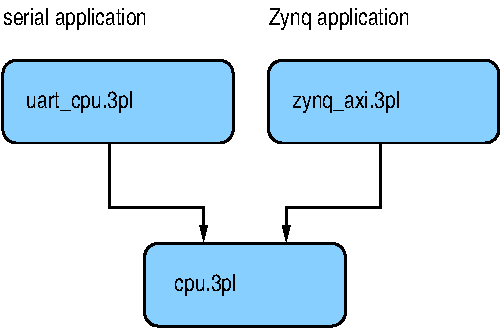
\includegraphics{cpu}

    xilinx/uart\_cpu.3pl is included in -\\
    boards/avnet/aes\_sp3a\_eval400.3pl\\
    board/gadget\_factory/papilio\_one\_100.3pl\\
    board/gadget\_factory/papilio\_one\_250.3pl\\
    board/gadget\_factory/papilio\_one\_500.3pl\\
    board/gadget\_factory/papilio\_pro\_lx4.3pl\\
    board/gadget\_factory/papilio\_pro\_lx9.3pl
    
    uart\_cpu begins by -
    
    \begin{lstlisting}[gobble=4, language=threepl]
    source "xilinx/cpu.3pl"         // CPU API classes file
    class(cpu, CPU_API());          // Create API class here as used below
    global function cpu_api () {    // Pass the API class to application code
        return(cpu);
    }
    \end{lstlisting}
    
    Since cpu.3pl is included via a source statement its code shares the scope
    of this library, UART\_CPU. Thus it can call the modules, functions and
    procedures therin.
    
    {\bf cpu.3pl} defines a class {\bf CPU\_API()} which provides the following
    class procedures for data transfer between FPGA and CPU - \\
        \hspace*{1cm}{\bf read()} generic read \autorefph{sec:lpcpurd} \\
        \hspace*{1cm}{\bf write()} generic write \autorefph{sec:lpcpuwr} \\
        \hspace*{1cm}{\bf read\_memory()} memory read \autorefph{sec:lpcpurdmem} \\
        \hspace*{1cm}{\bf read\_queue()} queue read \autorefph{sec:lpcpurdqueue} \\
        \hspace*{1cm}{\bf read\_value()} value read \autorefph{sec:lpcpurdvalue} \\
        \hspace*{1cm}{\bf write\_memory()} memory write \autorefph{sec:lpcpuwrmem} \\
        \hspace*{1cm}{\bf write\_queue()} queue write \autorefph{sec:lpcpuwrqueue} \\
        \hspace*{1cm}{\bf write\_static()} static write \autorefph{sec:lpcpuwrstat} \\
        \hspace*{1cm}{\bf dma\_read()} to FPGA from CPU \autorefph{sec:lpcpudmar} \\
        \hspace*{1cm}{\bf dma\_write()} from FPGA to CPU \autorefph{sec:lpcpudmaw} \\
        \hspace*{1cm}{\bf signal\_interrupt()} interrupt from a signal \autorefph{sec:lpcpusigint} \\
        \hspace*{1cm}{\bf interrupt()} interrupt procedure \autorefph{sec:lpcpuint} \\

    each of which can generate an instance of a CPU interface to a specific 3PL
    variable of appropriate mode. An internal class {\bf CPU\_CODEGEN} is also
    created but this is not visible to the application code 
    
    cpu.3pl is sourced by both {\bf uart\_cpu.3pl} and {\bf zynq\_axi.3pl} to
    provide CPU interfaces. The former employs a serial data link and the
    latter parallel busses.
    
    When any of the procedures above are called a defining structure is
    created which is added to a list of CPU interfaces. At the end
    of immediate execution module {\bf create\_bus\_interfaces()} is called.
    {\bf create\_bus\_interfaces()} is defined in both {\bf uart\_cpu.3pl}
    and {\bf zynq\_axi.3pl} as it is specific to each. This module
    traverses the interface list constructed above and for each interface
    calls a matching procedure in class {\bf CPU\_CODEGEN} to generate the
    logic for each instance.








    \subsection{library modules}
    



        \subsubsection{cpu\_interface - create the CPU interface low-level logic}\label{sec:lmuartcpui}

            {\bf Library: xilinx/uart\_cpu.3pl)}

            {\bf Prototype:} \\
            \vsp
            \begin{lstlisting}[gobble=12, language=threepl]
                module
                cpu_interface () {}
            \end{lstlisting}
            
            {\bf Output parameters:} \\
            
                none.                       
            
            {\bf Input parameters:} \\
            
                none.
                       
            {\bf description:} \\
            This module is called by module {\bf create\_bus\_interfaces}
            to generate the low-level interface logic to the CPU.




        \subsubsection{create\_bus\_interfaces - create the individual CPU interfaces}\label{sec:lmuartcpucbi}

            {\bf Library: xilinx/uart\_cpu.3pl)}

            {\bf Prototype:} \\
            \vsp
            \begin{lstlisting}[gobble=12, language=threepl]
                module
                create_bus_interfaces () {}
            \end{lstlisting}
            
            {\bf Output parameters:} \\
            
                none.                       
            
            {\bf Input parameters:} \\
            
                none.
                       
            {\bf description:} \\
            This module creates the logic for each of the CPU interfaces. Each
            of these communicates via logic created by module {\bf cpu\_interface}
            described above.







        \subsubsection{dma\_read - DMA read to the FPGA from CPU RAM}\label{sec:lmuartcpudmar}

            {\bf Library: xilinx/uart\_cpu.3pl)}

            {\bf Prototype:} \\
            \vsp
            \begin{lstlisting}[gobble=12, language=threepl]
                module
                dma_read (
                    queue(data)
                    <-
                    queue(address, "uint:16")   // relative memory address
                ) {}
            \end{lstlisting}
            
            {\bf Output parameters:} \\
            
                {\bf data} is the data output queue.                       
            
            {\bf Input parameters:} \\
            
                {\bf address} is a queue supplying the CPU RAM address
                relative to the DMA base address.
                       
            {\bf description:} \\
            This module performs a DMA read to the FPGA from CPU RAM. The
            transfer occurs when input queue {\bf address} is not empty
            and the output queue {\bf data} is not full.\\







        \subsubsection{dma\_write - DMA write from the FPGA to CPU RAM}\label{sec:lmuartcpudmaw}

            {\bf Library: xilinx/uart\_cpu.3pl)}

            {\bf Prototype:} \\
            \vsp
            \begin{lstlisting}[gobble=12, language=threepl]
                module
                dma_write (
                    queue(data),
                    queue(address, "uint:16")   // relative memory address
                ) {}
            \end{lstlisting}
            
            {\bf Output parameters:} \\
            
                none.                       
            
            {\bf Input parameters:} \\
                        
                {\bf data} is the data input queue.\\
                {\bf address} is a queue supplying the CPU RAM address
                relative to the DMA base address.\\
                       
            {\bf description:} \\
            This module performs a DMA write from the FPGA to CPU RAM. The
            transfer occurs when input queues {\bf address} and data are
            not empty.

        \subsubsection{sigint - interrupt the CPU on a signal}\label{sec:lmuartcpusigint}

            {\bf Library: xilinx/uart\_cpu.3pl)}

            {\bf Prototype:} \\
            \vsp
            \begin{lstlisting}[gobble=12, language=threepl]
                module
                sigint(int(n), value(sig, "log")) {}
            \end{lstlisting}
            
            {\bf Output parameters:} \\
            
                none.                       
            
            {\bf Input parameters:} \\
                        
                {\bf n} is the interrupt index, 0 to 16.\\
                {\bf sig} is a signal on whose rising edge the interrupt
                is triggered.\\
                       
            {\bf description:} \\
            When the signal {\bf sig} is asserted the interrupt is triggered.
            The interrupt number, 0 to 15, is given by {\bf index}.


    
    \subsection{library procedures}
            


        \subsubsection{add\_interface - add an interface to the interface list}\label{sec:lpuartcpuai}

            {\bf Library: xilinx/uart\_cpu.3pl)}

            {\bf Prototype:} \\
            \vsp
            \begin{lstlisting}[gobble=12, language=threepl]
                procedure
                add_interface (var(v, "->")) {}
            \end{lstlisting}
            
            {\bf Output parameters:} \\
            
                none.
                       
            {\bf Input parameters:} \\
            {\bf v} is an instance of class {\bf busCommon}, defined in
            cpu.3pl.
                     
            {\bf description:} \\
            The instance of {\bf busCommon} is added to the interface list.
            The list is processed at completion of immediate execution to
            create the whole CPU interface.


        \subsubsection{cpu\_read - write to CPU}\label{sec:lpuartcpurd}

            {\bf Library: xilinx/uart\_cpu.3pl)}

            {\bf Prototype:} \\
            \vsp
            \begin{lstlisting}[gobble=12, language=threepl]
                procedure
                cpu_read (
                    value(access, "log"),
                    value(init, "log"), 
                    queue(out)
                    <-
                    int(bus),
                    int(addr),
                    value(data_in),
                    value(contin, "log")
                ) {}
            \end{lstlisting}
            
            {\bf Output parameters:} \\
            {\bf access} is an optional output parameter which is asserted
            when a CPU to FPGA write occurs.\\
            {\bf init} is an output parameter which is asserted in the case
            of a memory read to initiate the read.\\
            {\bf out} is an optional queue variable which will be written to
            when a transfer occurs.\\

                       
            {\bf Input parameters:} \\
            {\bf bus} is not used (applies to Zynq).\\
            {\bf address} is a 6 bit interface address.\\
            {\bf data\_in} input data.\\
            {\bf contin} is only used for a memory read and is asserted
            when the memory read has occured and the transfer can begin.\\
                     
            {\bf description:} \\
            This procedure provides a low-level interface to transfer
            data from the FPGA to the CPU via the USB serial port. It is
            used by modules and procedures in library cpu.3pl and is not
            intended for use directly by application code.
            
            The CPU initiates the transfer. The transfer may consist of
            multiple bytes.


        \subsubsection{cpu\_write - write to CPU}\label{sec:lpuartcpuwr}

            {\bf Library: xilinx/uart\_cpu.3pl)}

            {\bf Prototype:} \\
            \vsp
            \begin{lstlisting}[gobble=12, language=threepl]
                procedure
                cpu_write (
                    var(out),
                    value(access, "log")
                    <-
                    int(bus),
                    int(addr)
                ) {}
            \end{lstlisting}
            
            {\bf Output parameters:} \\
            {\bf var} is a static or queue mode variable.\\          
            {\bf access} is an optional output parameter which is asserted
            when a CPU to FPGA write occurs.\\
                       
            {\bf Input parameters:} \\
            {\bf bus} is not used (applies to Zynq).\\
            {\bf address} is a 6 bit interface address.\\           
                     
            {\bf description:} \\
            This procedure provides a low-level interface to transfer
            data from the CPU to the FPGA via the USB serial port. It is
            used by modules and procedures in library cpu.3pl and is not
            intended for use directly by application code.
            
            The CPU initiates the transfer. The transfer may consist of
            multiple bytes.



    \subsection{library functions}

        \subsubsection{cpu\_api - CPU communications interface}\label{sec:lfcpuapi}

            {\bf Library: xilinx/uart\_cpu.3pl)}

            {\bf Prototype:} \\
            \vsp
            \begin{lstlisting}[gobble=12, language=threepl]
               global function
               cpu_api () {}
            \end{lstlisting}

            {\bf Return mode and type:} \\
            immediate, class

            {\bf Input parameters:} \\            
            
            none.
            
            {\bf description:} \\
            This function returns an instance of class CPU\_API














\pagebreak

\section{The Standard Library - stdlib.3pl}

    \index{library!stdlib.3pl}
    This library contains modules, procedures and functions common
    to all platforms.
    
    This library must be incorporated by using a {\bf module} statement -
    \begin{lstlisting}[gobble=4, language=threepl]
       module "stdlib.3pl"
    \end{lstlisting}
    
    This library includes {\bf multlib.3pl} and {\bf divlib.3pl}. These are
    not documented separately.

    \subsection{global structs}
        
%        Global struct {\em bram} is created for use with block RAM
%        extended access procedures {\em rwrite2()} and {\em rread2()} and
%        function {\em rmemoryout2()}.
%
%        \begin{lstlisting}[gobble=8, language=threepl]
%           struct(bram,
%               bwidth, "int",  // block data width (in 1st only)
%               twidth, "int",  // total data width (in 1st only)
%               block,  "->",   // memory block
%               next,   "->"    // next bram struct in linked list
%           );
%        \end{lstlisting}
%        
%        Global struct {\em mem\_ad} is created for use with external memory
%        access.
%
%        \begin{lstlisting}[gobble=8, language=threepl]
%           struct (mem\_ad,
%               address,    "uint:20",
%               data,       "bits:18"
%           );
%        \end{lstlisting}
%        
%        It is used by the modules {\bf extramread} and {\bf extramwrite}.
        
        Global structs {\bf ds16}, {\bf ds16e} and {\bf ds32} are
        used for block protocols and for high speed serial channel data.

        \begin{lstlisting}[gobble=8, language=threepl]
           struct(global.ds16,
               data,   "bits:16",  // data word
               k,      "log"       // data word contains K-character in MS byte
           );
        \end{lstlisting}

        \begin{lstlisting}[gobble=8, language=threepl]
           struct(global.ds16e,
               data,   "bits:16",  // data word
               k,      "log",      // data word contains K-character in MS byte
               error,  "log"       // data word is erroneous
           );
        \end{lstlisting}

        \begin{lstlisting}[gobble=8, language=threepl]
           struct(global.ds32,
               data,   "uint:32",  // data word
               k,      "log"       // data word contains K-character in MS byte
           );
        \end{lstlisting}


    \subsection{library modules}
    
        \subsubsection{array\_to\_queue - serialise an array to a
                                                    queue}\label{sec:lmarraytoqueue}


            {\bf Library: stdlib.3pl}

            {\bf Prototype:} \\
            \vsp
            \begin{lstlisting}[gobble=12, language=threepl]
               global module
               array_to_queue (
                   queue(pout),
                   value(busy, "log")
                   <-
                   value(in),
                   value(enable),
                   value(go, "log")
               );
            \end{lstlisting}

            {\bf Output parameters:} \\
            {\bf pout} is the output queue variable\\
            {\bf busy} is true when the module cannot accept another input

            {\bf Input parameters:} \\
            {\bf in} is the input array.\\
            {\bf enable} is an optional argument controlling the number of
            items in {\bf in} to process.\\
            {\bf go} is asserted to trigger the serialisation.

            {\bf description:} \\
            Parameter {\bf in} is an array. It may be value, static, queue,
            selectvalue or priority mode.
            
            Parameter {\bf enable} is a one dimensional array of "log" and may
            be value, static, or selectvalue mode. It must have the same
            dimension as the first or only dimension of parameter {\bf in}.            
            
            When {\bf go} is true the input array is copied to an internal
            structure which is then shifted out to the output queue {\bf pout}.
            The {\bf enable} array indicates which members of array {\bf in} are
            to be copied and shifted, the lowest index false member of {\bf
            enable} indicating that all members of array {\bf in} from that
            index up are ignored. Thus array {\bf enable} must have a number of
            contiguous entries which are true, starting at index 0, and that
            selects the number of contiguous entries in array {\bf in} which
            will be copied and shifter to the output queues, again starting with
            index 0. {\bf go} may contain queue reads.
            
            The second input argument, for parameter {\bf enable}, may be
            omitted in which case all members of {\bf in} will be shifted and
            copied to the output queue.
            
            The output queue must be the same type as the input
            array members. While the serialisation is in progress output value
            {\bf busy} is true. If input {\bf go} is true when {\bf busy} returns to
            false another conversion will take place. If the input {\bf in} is a queue
            then {\bf go} may be held true.
            
            The serialisation takes a number of clock cycles equal to the number
            of entries in the input array that are enabled plus one and hence
            the input data rate is limited to $\frac{1}{n+1}$ where $n$ is the
            number of enabled entries in the input array.



    
        \subsubsection{crc\_8\_16 - 16 bit CRC from 8 bit data}\label{sec:lmcrc816}


            {\bf Library: stdlib.3pl}

            {\bf Prototype:} \\
            \vsp
            \begin{lstlisting}[gobble=12, language=threepl]
               global module
               crc_8_16 (
                   static(out, "uint:16")
                   <-
                   queue(in, "uint:8"),
                   str(poly, "CRC16")
               ) {}
            \end{lstlisting}

            {\bf Output parameters:} \\
            {\bf out} is the output static variable.

            {\bf Input parameters:} \\
            {\bf in} is the input queue.\\
            {\bf poly} is an optional string argument to select the polynomial
            used.

            {\bf description:} \\
            This module accumulate a 16 bit CRC from 8 bit data. Parameter {\bf
            in} is the data input queue, type "uint:8". The CRC is updated as
            each input datum is read. The optional parameter {\bf poly} selects
            one of two polynomials to use. "CRC16" (default) selects $x^{16} +
            x^{15} + x^{13} + 1$. "CCITT" selects $x^{16} + x^{12} + x^5 + 1$. parameter
            {\bf out} is a "uint:16" static variable in which the CRC value is
            accumulated Input data can be read at clock rate.



    
        \subsubsection{crc\_16\_16 - 16 bit CRC from 8 bit data}\label{sec:lmcrc1616}


            {\bf Library: stdlib.3pl}

            {\bf Prototype:} \\
            \vsp
            \begin{lstlisting}[gobble=12, language=threepl]
               global module
               crc_16_16 (
                   static(out, "uint:16")
                   <-
                   queue(in, "uint:16"),
                   str(poly, "CRC16")
               ) {}
            \end{lstlisting}

            {\bf Output parameters:} \\
            {\bf out} is the output static variable.

            {\bf Input parameters:} \\
            {\bf in} is the input queue.\\
            {\bf poly} is an optional string argument to select the polynomial
            used.

            {\bf description:} \\
            This module accumulate a 16 bit CRC from 16 bit data. Parameter {\bf
            in} is the data input queue, type "uint:16". The CRC is updated as
            each input datum is read. The CRC is computed successively from each
            8-bit half of each input datum but in one clock cycle. The optional
            parameter {\bf poly} selects one of two polynomials to use. "CRC16"
            (default) selects $x^{16} + x^{15} + x^{13} + 1$. "CCITT" selects
            $x^{16} + x^{12} + x^5 + 1$. parameter {\bf out} is a "uint:16"
            static variable in which the CRC value is accumulated Input data can
            be read at clock rate.








    
        \subsubsection{crcblock - block 32 bit data with a CRC}\label{sec:lmcrcblock}


            {\bf Library: stdlib.3pl}

            {\bf Prototype:} \\
            \vsp
            \begin{lstlisting}[gobble=12, language=threepl]
               global module
               crcblock (
                   queue(out, ds16)
                   <-
                   queue(in, ds32),
                   int(max_blk_len, 20),
                   int({sob, eob}),
                   log(fixed)
               ) {}
            \end{lstlisting}

            {\bf Output parameters:} \\
            {\bf out} is the output queue, type ds16.

            {\bf Input parameters:} \\
            {\bf in} is the input queue, type ds32.\\
            {\bf max\_blk\_len} is the maximum variable block size or the fixed
                    block size.\\
            {\bf sob} is the start-of-block K-character to be used.\\
            {\bf eob} is the end-of-block K-character to be used.\\
            {\bf fixed} is an optional logical argument to select fixed
                    length blocks.

            {\bf description:} \\
            This module encloses data in a block containing a cyclic reduncancy
            check word. The 16 bit CRC polynomial is $x^{16} + x^{15} + x^{13} +
            1$. Blocks can be fixed or variable length.

            When input data become available the start-of-block word is written
            to the output queue. The start-of-block word has the most significant
            byte set to the start-of-block K character, the least significant
            byte to zero and the K flag is true. If 'fixed' is false (default),
            incoming data is read until either unavailable or max\_block\_len
            items have been read and the block is then terminated. If 'fixed' is
            true, incoming data is read until max\_block\_len items have been
            read and the block is then terminated. each 32 bit word is written
            to the output as a pair of 16 bit words. A 16 bit CRC is accumulated
            from each 16 bit data word. When the block is terminated the 16 bit
            CRC is written to the output followed by an end-of-block word. The
            end-of-block word has the most significant byte set to the
            end-of-block K character, the least significant byte to zero and the
            K flag is true.

            \begin{tabular}{| c | c | c | l}
            \cline{1-3}
            K & upper & lower & \\
            flag & byte & byte & \\
            \cline{1-3}
            \cline{1-3}
            1 & sob &  0  & start-of-block \\ \cline{1-3}
            0 & \multicolumn{2}{| c |}{data word 1} & first data word \\ \cline{1-3}
            0 & \multicolumn{2}{| c |}{data word 2} & second data word \\ \cline{1-3}
            . & \multicolumn{2}{| c |}{.} &  \\
            . & \multicolumn{2}{| c |}{.} &  \\ \cline{1-3}
            0 & \multicolumn{2}{| c |}{data word n} & last data word \\ \cline{1-3}
            0 & \multicolumn{2}{| c |}{CRC} & CRC \\ \cline{1-3}
            1 & eob &  0  & end-of-block \\ \cline{1-3}
            \end{tabular}








    
        \subsubsection{crcunblock - unblock 32 bit data with a CRC}\label{sec:lmcrcunblock}


            {\bf Library: stdlib.3pl}

            {\bf Prototype:} \\
            \vsp
            \begin{lstlisting}[gobble=12, language=threepl]
               global module
               crcunblock (
                   queue(dout, ds32),
                   static(eout)
                   <-
                   queue(in, ds16),
                   int(max_blk_len, 20),
                   int({sob, eob})
               ) {}
            \end{lstlisting}

            {\bf Output parameters:} \\
            {\bf out} is the output queue, type ds32.\\
            {\bf eout} is an optional error counter static variable.

            {\bf Input parameters:} \\
            {\bf in} is the input queue, type ds16.\\
            {\bf max\_blk\_len} is the maximum variable block size or the fixed
                    block size.\\
            {\bf sob} is the start-of-block K-character to be used.\\
            {\bf eob} is the end-of-block K-character to be used.

            {\bf description:} \\
            This module unwraps data from a block containing a cyclic reduncancy
            check word. The 16 bit CRC polynomial is $x^{16} + x^{15} + x^{13} +
            1$. Blocks can be fixed or variable length. The start-of-block word,
            CRC word and end-of-block word are stripped off the input stream and
            data words are packed into 32 bit words (ds32 struct). A CRC is
            computed from the block data including the transmitted CRC word. If
            the resulting CRC is zero the block is written to the output queue.
            If the CRC is not zero the block is discarded.
            
            When a block CRC error is encountered if the output parameter 'eout'
            has an argument the data length of the discarded block is added to
            the value of that variable. Any words received that do not match the
            block format cause 'eout' to be incremented. The size of the 'eout'
            counter is determined by the argument passed in the call to
            crcunblock().

            If the block length exceeds the maximum block length the block is
            terminated and discarded and if the optional error counter output
            parameter is used, the block length is added to the error count.

            Unpacked data is written to a dual-port circular buffer so that
            completed correct data words can be copied to the output data queue
            in parallel with unpacking of incoming blocks. If the output queue
            becomes unavailable for writing, data words will be discarded.


    
  
        \subsubsection{cread - read combinatorial output memory to a
                                                        queue}\label{sec:lmcread}

            {\bf Library: stdlib.3pl}


            {\bf Prototype:} \\
            \vsp
            \begin{lstlisting}[gobble=12, language=threepl]
               global module
               cread (queue(data) <- rmemory(m), int(port), queue(addr)) {}
            \end{lstlisting}

            {\bf Output parameters:} \\
            {\bf data} is the queue variable to be written to from the memory
            read. It takes its type from the argument.

            {\bf Input parameters:} \\
            {\bf m} is the memory.\\
            {\bf port} is the memory port.\\
            {\bf addr} is the memory address.

            {\bf description:} \\
            Read the combinatorial output memory when the input and output
            queues are available. The program logic must ensure that this
            memory port access is mutually exclusive to all other accesses
            to that port.
            
            This module is just a wrapper around a single statement. The source
            is
            \begin{lstlisting}[gobble=12, language=threepl]
               global module
               cread (queue(data) <- rmemory(m), int(port), queue(addr)) {
                   data <<- cast(cmemoryread(m, port, addr), type(data));
               }
            \end{lstlisting}
                        
            It is provided to complete the set {\bf cread()}, {\bf cwrite()},
            {\bf rread()} and {\bf rwrite()} where only rread() contains
            significant code.
            
            See also - \\
            {\bf cwrite()} \autorefph{sec:lmcwrite}, \\
            {\bf rread()} \autorefph{sec:lmrread}, \\
            {\bf rwrite()} \autorefph{sec:lmrwrite}.

    
        \subsubsection{cwrite - write combinatorial output memory from a
                                                    queue}\label{sec:lmcwrite}

            {\bf Library: stdlib.3pl}

            {\bf Prototype:} \\
            \vsp
            \begin{lstlisting}[gobble=12, language=threepl]
               global module
               cwrite (rmemory(m), int(port), queue({addr, data})) {}
            \end{lstlisting}

            {\bf Output parameters:} \\
            none

            {\bf Input parameters:} \\ 
            {\bf m} is the memory.\\
            {\bf port} is the memory port.\\
            {\bf addr} is the memory address.\\            
            {\bf data} is the data to be written.

            {\bf description:} \\
            Write to the combinatorial output memory when the input queues are
            available. The program logic must ensure that this memory port
            access is mutually exclusive to all other accesses to that port.
            
            This module is just a wrapper around a single statement. The source
            is
            \begin{lstlisting}[gobble=12, language=threepl]
               global module
               cwrite (rmemory(m), int(port), queue(addr), queue(data)) {
                   cmemorywrite(m, port, addr, data);
               }
            \end{lstlisting}
                        
            It is provided to complete the set {\bf cread()}, {\bf cwrite()},
            {\bf rread()} and {\bf rwrite()} where only rread() contains
            significant code.
            
            See also - \\
            {\bf cread()} \autorefph{sec:lmcread}, \\
            {\bf rread()} \autorefph{sec:lmrread}, \\
            {\bf rwrite()} \autorefph{sec:lmrwrite}.





        \subsubsection{demultiplex - demultiplex a source\\
                    demultiplex\_l - demultiplex a source using port bit\\
                    demultiplex\_e - demultiplex a source using port number}\label{sec:lmdemultiplex}

            {\bf Library: stdlib.3pl}

            {\bf Prototypes:} \\
            \vsp
            \begin{lstlisting}[gobble=12, language=threepl]
               global module
               demultiplex.... (varargs <- queue(in)) {}
            \end{lstlisting}

            {\bf Output parameters:} \\
            {\bf varargs} any number of output sinks, an array of pointers
            to sinks or a list of sinks.

            {\bf Input parameters:} \\
            {\bf in} is a single input queue.

            {\bf description:} \\
            These modules are intended to demultiplex a single input queue to a
            number of output queues. Outputs need not be the same type but they must
            be assignable from the input type (or {\bf body} field of the input -
            see below). The input need not contain queue reads in which case it will
            be read on every clock cycle.

            These modules may also be called with a single output argument which
            is an array of pointers to queues. In this case they behave as though
            called with the queues as separate arguments. Similarly the single
            output argument may be of type "list", the list containing pointers
            to queues.

            The output types must be a type assignable from the input data
            type. By 'assignable' is meant that the types need not be identical,
            e.g. the number of bits may differ in which case truncation or
            padding will occur or a "uint" may be assigned to an "int".

            For {\bf demultiplex()} the input can be any type. The input is
            copied to the outputs in turn. If an output is not available the
            next available output in cyclic order is selected. If no outputs
            are available the module waits until any output is available and
            this is written to.

            For {\bf demultiplex\_l()} the input type is a wrapper struct
            containing the datum and an output port identifier. That identifier
            is an array of type "log" in which one member is {\bf true} to
            identify the output port. The struct can be created by calling the
            library global function {\bf multiplex\_struct\_l()}
            \autorefph{sec:lfmultiplexstruct}.

            For {\bf demultiplex\_e()} the input type is a wrapper struct
            containing the datum and an output port identifier. That identifier
            is  a "uint" containing the port number (starting at 0). The struct
            can be created by calling the library global function {\bf
            multiplex\_struct\_e()} \autorefph{sec:lfmultiplexstruct}.

            If the selected output queue is an unmatched parameter then the input is
            still read but the data is discarded. For {\bf demultiplex\_l()} and
            {\bf demultiplex\_e()} the directive "demultiplex\_skip\_null\_outputs"
            can be set to true to ignore any unmatched output parameters, but note
            that if an input is directed to that output port the input will not be
            read.

            These modules read and write in the current clock domain.
            Input and output queues may be asynchronous.
            
            The module {\bf demultiplex()} operates by means of a token placed
            on one output. When the input becomes available the first available
            output downstream of the token is written and the token is moved to
            the output following the one written. There are no clock cycles
            lost, as in a traditional token ring, in waiting for the token to
            move around the ring to an available output, thus the module is
            capable of forwarding an input datum on every clock cycle. The
            implementation uses the Xilinx carry chain to minimise the delay
            through the logic cascade of the token ring. If the carry chain were
            not used the logic delays would severely limit the clock rate at
            which this module could be used. Modules {\bf demultiplex\_l()} and
            {\bf demultiplex\_e()} do not need the token ring as the required
            output is explicitly specified by the input.

            
            See also - \\
            {\bf multiplex()} \autorefph{sec:lmmultiplex} \\
            {\bf multiplex\_l()} \autorefph{sec:lmmultiplex} \\
            {\bf multiplex\_e()} \autorefph{sec:lmmultiplex} \\
            {\bf multiplexp()} \autorefph{sec:lmmultiplex} \\
            {\bf multiplexp\_l()} \autorefph{sec:lmmultiplex} \\
            {\bf multiplexp\_e()} \autorefph{sec:lmmultiplex} \\
            {\bf multiplext()} \autorefph{sec:lmmultiplex} \\
            {\bf multiplext\_l()} \autorefph{sec:lmmultiplex} \\
            {\bf multiplext\_e()} \autorefph{sec:lmmultiplex} \\
            {\bf multiplex\_struct\_l()} \autorefph{sec:lfmultiplexstruct} \\
            {\bf multiplex\_struct\_e()} \autorefph{sec:lfmultiplexstruct}.



        \subsubsection{divide - pipeline divide}\label{sec:lmdivide}

            {\bf Library: stdlib.3pl}

            {\bf Prototype:} \\
            \vsp
            \begin{lstlisting}[gobble=12, language=threepl]
               global module
               divide (queue(quot), queue(rem) <- value(num), value(denom)) {}
            \end{lstlisting}

            {\bf Output parameters:} \\
            {\bf quot} is the quotient.\\
            {\bf rem} is the remainder.

            {\bf Input parameters:} \\
            {\bf num} is the dividend.\\
            {\bf denom} is the divisor.
            
            This module is in divlib.3pl which is included in stdlib.3pl.

            {\bf description:} \\
            This module is a pipeline divider. The numerator and denominator
            arguments may be int, uint, int:, uint:, fixed: or ufixed: where the
            trailing ":" indicates target types. For integer types the quotient
            and remainder outputs are integer, signed if either input is signed,
            and either or both the quotient and remainder outputs may be used.
            For one or both inputs fixed point the quotient output will be fixed
            point, signed if either input is signed, and the remainder output
            is not used.
            
            If neither input is a queue or an expression containing a queue the
            divider will accept input on every clock cycle. Either input may be
            immediate mode but both inputs must not be immediate mode. The
            quotient and remainder will become available at the outputs after a
            latency which is determined by the numerator width. Data in transit
            through the module will continue to the outputs regardless of the
            availability of further input data.

            The remainder queue output argument should be at least as wide as the
            denominator argument otherwise the resulting truncation may lose
            data (if the range is known to be constrained then this is
            acceptable).

            For unsigned integer divide (both numerator and denominator
            arguments unsigned target types or non-negative immediate) the
            result width is the width of the numerator argument.

            For signed integer divide (either or both numerator or denominator
            arguments int target types or negative immediate) the result width
            will be one bit wider than for unsigned divide. The extra bit is
            only required for the single case where both numerator and
            denominator are the maximum negative values (e.g. -8 / -1 gives +8,
            but -8 has a width of 4 bits and +8 as a signed int has a width of 5
            bits). If this case is known not to arise a narrower output queue may
            be used.
            
            For fixed point divide the result width is the sum of the numerator
            and denominator widths and the result binary point offset is
            the numerator offset + denominator width - denominator offset.

            The number of pipeline stages is equal to the number of bits in the
            numerator plus one.

            Divide by zero is not detected and gives an undefined result.





        \subsubsection{fifo - a fifo with static interface}\label{sec:lmfifo}

            {\bf Library: stdlib.3pl}

            {\bf Prototype:} \\
            \vsp
            \begin{lstlisting}[gobble=12, language=threepl]
               global module
               fifo (
                   value(out), value({emptyout, fullout}, "log")
                   <-
                   value(in), value({read, write}, "log")
               ) {}
            \end{lstlisting}

            {\bf Output parameters:} \\
            {\bf out} is the data output for a fifo read.\\
            {\bf emptyout} is true if the fifo is empty.\\
            {\bf fullout} is true if the fifo is full.

            {\bf Input parameters:} \\
            {\bf in} is the data input for a fifo write.\\
            {\bf read} causes a fifo read on a clock cycle when high.\\
            {\bf write} causes a fifo write on a clock cycle when high.

            {\bf description:} \\
            Read or write a fifo. On each clock cycle {\bf emptyout} and {\bf
            fullout} indicate when reads and writes respectively cannot be
            executed. The program must ensure that these conditions are
            checked as the module does not do so! If {\bf read} or {\bf
            write} are high in a clock cycle then a read or write will be
            performed. These can be done on the same clock cycle.





        \subsubsection{multiplex - multiplex sources\\
                    multiplex\_l - multiplex sources giving port bit\\
                    multiplex\_e - multiplex sources giving port number\\
                    multiplexp - multiplex queues with priority\\
                    multiplexp\_l - multiplex queues with priority giving port bit\\
                    multiplexp\_e - multiplex queues with priority giving port number\\
                    multiplext - multiplex queues via a tree\\
                    multiplext\_l - multiplex queues via a tree giving port bit\\
                    multiplext\_e - multiplex queues via a tree giving port number}\label{sec:lmmultiplex}

            {\bf Library: stdlib.3pl}

            {\bf Prototype:} \\
            \vsp
            \begin{lstlisting}[gobble=12, language=threepl]
               global module
               multiplex.... (queue(out) <- varargs) {}
            \end{lstlisting}

            {\bf Output parameters:} \\
            {\bf out} is a single output queue.

            {\bf Input parameters:} \\
            {\bf varargs} any number of input sources, an array of pointers
            to sources or a list of sources.

            {\bf description:} \\
            These modules are intended to multiplex a number of input queues to a
            single output queue. Inputs need not be the same type but they must
            be assignable to the output type (or {\bf body} field of the output
            queue - see below). By 'assignable' is meant that the types need not
            be identical, e.g. the number of bits may differ in which case
            truncation or padding will occur or a "uint" may be assigned to an
            "int".          
            
            When inputs become available simultaneously modules {\bf
            multiplex()}, {\bf multiplex\_l()} and {\bf multiplex\_e()} use a
            pseudo-token ring to give equal treatment to all inputs. Note that
            although these modules were written to multiplex queues (or more
            correctly expressions containing queue reads), the input arguments
            could be other modes, say value or static. Where no queue reads are
            involved an expression is always available. In that case the inputs
            would be sampled and copied to the output queue continuously in a
            cyclic order. In principle the inputs could be a mixture of modes in
            which case they would be read cyclically but a queue would be skipped
            if not available for reading.

            Modules {\bf multiplexp()}, {\bf multiplexp\_l()} and {\bf
            multiplexp\_e()} handle simultaneous inputs by choosing the
            left-most available queue in the argument list. For these modules the
            inputs must contain queue reads.

            Modules {\bf multiplext()}, {\bf multiplext\_l()} and {\bf
            multiplext\_e()} handle simultaneous inputs by means of a balanced tree
            structure.
            
            All nine modules may also be called with a single input argument
            which is an array of pointers to sources. In this case they behave
            as though called with the sources as separate arguments. Similarly
            the single input argument may be of type "list", the list containing
            pointers to sources.
            
            In many applications it is necessary to be able to identify the
            origin of an output datum, i.e. the input argument to the module
            from which the datum was read. To facilitate this the module output
            queue type may be a struct which is a wrapper containing the output
            datum and an input port identifier. The output type for {\bf
            multiplex()} and {\bf multiplexp()} do not use a wrapper type, the
            output type being directly compatible with the input type(s).
            
            The output type for {\bf multiplex\_l()}, {\bf multiplexp\_l()} and
            {\bf multiplext\_l()} is a wrapper with two field, {\bf body}
            containing the datum and {\bf port}  which is an array of type "log"
            in which one member is {\bf true} to identify the input port. The
            struct can be created by calling the library global function {\bf
            multiplex\_struct\_l()} \autorefph{sec:lfmultiplexstruct}.
            
            The output type for {\bf multiplex\_e()}, {\bf multiplexp\_e()} and
            {\bf multiplext\_e()} is a wrapper with two fields, {\bf body}
            containing the datum and {\bf port}  which is a "uint" containing
            the port number (starting at 0). The struct can be created by
            calling the library global function {\bf multiplex\_struct\_e()}
            \autorefph{sec:lfmultiplexstruct}.
            
            In the case of {\bf multiplex()}, {\bf multiplexp()} and {\bf
            multiplext()} the inputs are copied to the output queue when
            available. For {\bf multiplex\_l()}, {\bf multiplexp\_l()} and {\bf
            multiplext\_l()} the selected input is copied to the {\bf body}
            field output queue when available and the associated port field has
            the member of the array indexed by the port number assigned true.
            For {\bf multiplex\_e()}, {\bf multiplexp\_e()} and {\bf
            multiplext\_e()} the same applies except that the port number is
            assigned to the "uint" {\bf port} field.
            
            The modules read and write in the current clock domain. Input
            and output queues may be asynchronous.
            
            The modules {\bf multiplex()}, {\bf multiplex\_l()} and {\bf
            multiplex\_e()} operate by means of a token placed on one input.
            When one or more inputs become available the first input downstream
            of the token is read and the token is moved to the input following
            the one read. There are no clock cycles lost, as in a traditional
            token ring, in waiting for the token to move around the ring to an
            available input, thus the module is capable of forwarding an input
            datum on every clock cycle. The implementation uses the Xilinx carry
            chain to minimise the delay through the logic cascade of the token
            ring. Unfortunately the carry chain must be circular and the link
            back from the top of a linear carry chain to the bottom introduces
            a significant delay. The propagation time around the token ring
            is large enough to severely lower the clock rate that can be used
            as the number of inputs increases.
            
            The modules {\bf multiplexp()}, {\bf multiplexp\_l()} and {\bf
            multiplexp\_e()} use a priority mode variable to select which input
            to read. For FPGAs priority mode variables are implemented using the
            Xilinx carry chain if the number of inputs exceeds the maximum
            number of LUT inputs. This is to minimise the delay through cascaded
            logic.
            
            The modules {\bf multiplext()}, {\bf multiplext\_l()} and {\bf
            multiplext\_e()} use a balanced tree with nodes of degree 2 to
            converge the inputs to the output. Each tree node arbitrates between
            its two inputs based on the number of leaves converging on each
            branch. The disadvantage of this scheme is that arbitration is
            based on the fixed configuration, not on the traffic through
            each branch. For example a four input multiplexer where
            input 4 is idle will arbitrate among the other three unfairly
            giving input 3 half the clock cycles, inputs 1 and 2 sharing the
            other half. The advantage of this multiplexer is that it will
            operate at a high clock rate since the arbitration is local to
            the nodes.
                        
            See also - \\
            {\bf demultiplex()} \autorefph{sec:lmdemultiplex} \\
            {\bf demultiplex\_l()} \autorefph{sec:lmdemultiplex} \\
            {\bf demultiplex\_e()} \autorefph{sec:lmdemultiplex} \\
            {\bf multiplex\_struct\_l()} \autorefph{sec:lfmultiplexstruct} \\
            {\bf multiplex\_struct\_e()} \autorefph{sec:lfmultiplexstruct}.
        




        \subsubsection{multiply - pipelined multiply}\label{sec:lmmultiply}

            {\bf Library: stdlib.3pl}

            {\bf Prototype:} \\
            \vsp
            \begin{lstlisting}[gobble=12, language=threepl]
               global module
               multiply (queue(prod) <- value(m1), value(m2)) {}
            \end{lstlisting}

            {\bf Output parameters:} \\
            {\bf prod} is the product.

            {\bf Input parameters:} \\
            {\bf m1} is the multiplicand.\\
            {\bf m2} is the multiplier.
            
            This module is in multlib.3pl which is included in stdlib.3pl.

            {\bf description:} \\
            This module is a pipeline multiplier for signed or unsigned
            integers. The module is useful for Virtex, Virtex E and Spartan 2
            FPGAs which do not contain hardware multipliers. Later Virtex and
            Spartan3 FPGAs containing hardware multipliers offer no reason to
            use this module.
            
            If neither input is a queue or an expression containing a queue the
            multiplier will accept input on every clock cycle unless the output
            queue becomes unavailable. Either input may be a constant but both
            inputs must not be constant. If either input is signed (a target int
            or a -ve constant) the output queue must be signed (an int, not a
            uint).

            The product will become available at the output after a latency
            which is determined by the input widths. Data in transit through the
            module will continue to the output regardless of the availability of
            further input data. The number of pipeline stages depends on the
            size and types of input arguments as follows -

            \begin{tabular}{ l l l }
            unsigned  & expr x expr     & bits in smallest expr \\
            signed    & expr x expr     & bits in smallest expr + 1 \\
            unsigned  & expr x constant & 1-bits in constant \\
            signed    & expr x constant & 1-bits in constant + 1 \\
            \end{tabular}
            
            where signed means that either input argument is signed. {\bf
            expr} means a target variable or expression, possibly containing
            queues. {\bf constant} means an immediate constant, variable or
            expression. Either input argument may be the constant.
            
            The width of the output queue argument should be at least the sum
            of the widths of the two input arguments. If narrower the result
            will be truncated at the most significant end. If the range of
            the product is known to be constrained then truncation of the
            product is acceptable.
            
            


        \subsubsection{pfifo - a prewrite fifo with static interface}\label{sec:lmpfifo}

            {\bf Library: stdlib.3pl}

            {\bf Prototype:} \\
            \vsp
            \begin{lstlisting}[gobble=12, language=threepl]
               global module
               pfifo (
                   value(out),
                   value({emptyout, fullout}, "log")
                   <-
                   value(in),
                   value({read, prewrite, write}, "log"),
                   value(reset, "log")
               ) {}
            \end{lstlisting}

            {\bf Output parameters:} \\
            {\bf out} is the data output for a fifo read.\\
            {\bf emptyout} is true if the fifo is empty.\\
            {\bf fullout} is true if the fifo is full.

            {\bf Input parameters:} \\
            {\bf in} is the data input for a fifo write.\\
            {\bf read} causes a fifo read on a clock cycle when high.\\
            {\bf prewrite} notifies the fifo that a write will be done
            in the future, reserving a place. When no free places remain the
            full condition will be come true.\\
            {\bf write} causes a fifo write on a clock cycle when high. The
            empty condition takes account of data actually written, not
            notified writes (prewrites).\\
            {\bf reset} is an optional reset to clear the fifo.

            {\bf description:} \\
            This fifo is intended to be used where data is to be passed
            through a fifo but there is a delay between execution of the
            data-producing operation and availability of that data. An
            example of this is external memory reads where the data only
            becomes available a number of cycles after the read command has
            been sent. The resulting data are then to be buffered in this
            fifo. To ensure that the memory reads can be pipelined it is
            necessary to notify the fifo that a write will occur later so
            that its test for space can take that into account. Once the
            memory read has been signaled it cannot be stopped so the fifo
            must have space available for the resulting datum some cycles
            later.
            
            On each clock cycle {\bf emptyout} and {\bf fullout} indicate
            when reads and writes respectively cannot be executed. The
            program must ensure that these conditions are checked as the
            module does not do so! If {\bf read}, {\bf prewrite} or {\bf
            write} are high in a clock cycle then a read, prewrite or write
            will be performed. Any combination of these can all occur on
            one clock cycle.


        \subsubsection{pdelay - delay pipeline data}\label{sec:lmpdelay}

            {\bf Library: stdlib.3pl}

            {\bf Prototype:} \\
            \vsp
            \begin{lstlisting}[gobble=12, language=threepl]
               global module
               pdelay (
                   queue(out)
                   <-
                   queue(in),
                   int(delay),
                   value(reset, "log")
               ) {}
            \end{lstlisting}

            {\bf Output parameters:} \\
            {\bf out} is the data output.

            {\bf Input parameters:} \\
            {\bf in} is the data input.\\
            {\bf delay} is the numnber of data to be delayed.\\
            {\bf reset} is an optional reset.

            {\bf description:} \\
            This module delays data by the number specified by argument
            {\bf delay}. The module will only operate when both input
            and output queues are available. Initially {\em delay} input data
            will be consumed while outputing default values (0, false etc.).
            Following this the output datum will be that input {\em delay}
            data cycles ago. The optional reset can be used to return the
            module to its initial condition.


        \subsubsection{rread - read registered output memory to a
                                                    queue}\label{sec:lmrread}

            {\bf Library: stdlib.3pl}

            {\bf Prototype:} \\
            \vsp
            \begin{lstlisting}[gobble=12, language=threepl]
               global module
               rread (queue(data) <- rmemory(m), int(port), queue(addr)) {}
            \end{lstlisting}

            {\bf Output parameters:} \\
            {\bf data} is the queue variable to be written to from the memory
            read. It takes its type from the argument.

            {\bf Input parameters:} \\
            {\bf m} is the memory.\\
            {\bf port} is the memory port.\\
            {\bf addr} is the memory address.

            {\bf description:} \\
            Read the registered output memory when the input and output
            queues are available. There is a latency of 2 cycles between input
            and output.
            
            The program logic must ensure that this
            memory port access is mutually exclusive to all other accesses
            to that port.
            
            See also - \\
            {\bf cread()} \autorefph{sec:lmcread}, \\
            {\bf cwrite()} \autorefph{sec:lmcwrite}, \\
            {\bf rwrite()} \autorefph{sec:lmrwrite}.


        \subsubsection{rwrite - write registered output memory from a
                                                    queue}\label{sec:lmrwrite}

            {\bf Library: stdlib.3pl}

            {\bf Prototype:} \\
            \vsp
            \begin{lstlisting}[gobble=12, language=threepl]
               global module
               rwrite (rram(m), int(port), queue({addr, data})) {}
            \end{lstlisting}

            {\bf Output parameters:} \\
            none

            {\bf Input parameters:} \\
            {\bf m} is the memory.\\
            {\bf port} is the memory port.\\
            {\bf addr} is the memory address.\\            
            {\bf data} is the data to be written.

            {\bf description:} \\
            Write to the registered output memory when the input queues are
            available. The program logic must ensure that this memory port
            access is mutually exclusive to all other accesses to that port.

            The registered output of the port is also changed to the written
            value.
            
            This module is just a wrapper around a single statement. The source
            is
            \begin{lstlisting}[gobble=12, language=threepl]
               global module
               rwrite (rmemory(m), int(port), value(addr), value(data)) {
                   rmemorywrite(m, port, addr, data);
               }
            \end{lstlisting}
                        
            It is provided to complete the set {\bf cread()}, {\bf cwrite()},
            {\bf rread()} and {\bf rwrite()} where only rread() contains
            significant code.
            
            See also - \\
            {\bf cread()} \autorefph{sec:lmcread}, \\
            {\bf cwrite()} \autorefph{sec:lmcwrite}, \\
            {\bf rread()} \autorefph{sec:lmrread}.


        \subsubsection{sort - generate a parallel Batcher sort network}\label{sec:lmsort}

            {\bf Library: stdlib.3pl}

            {\bf Prototype:} \\
            \vsp
            \begin{lstlisting}[gobble=12, language=threepl]
               global module
               sort (queue(out) <- queue(in)) {}
            \end{lstlisting}

            {\bf Output parameters:} \\
            {\bf out} is the output queue.

            {\bf Input parameters:} \\
            {\bf in} is the input queue.

            {\bf description:} \\
            This module generates a parallel sort network. The input and output
            arguments are queues which are 1-dimensional arrays of type uint or
            int. The output ordering depends on the The input and output array
            dimensions and types must be the same. The number of pipeline
            stages in this module depends on the dimensions of the queues. The
            sort network is generated using Batcher's algorithm. Note that the
            amount of logic used grows rapidly with the dimensionality of the
            queues!



        \subsubsection{sqrt - target fixed point square root}\label{sec:lmsqrt}

            {\bf Library: stdlib.3pl}

            {\bf Prototype:} \\
            \vsp
            \begin{lstlisting}[gobble=12, language=threepl]
               global module
               sqrt (queue(out) <- queue(in)) {}
            \end{lstlisting}

            {\bf Output parameters:} \\
            {\bf out} is the output queue.

            {\bf Input parameters:} \\
            {\bf in} is the input queue.

            {\bf description:} \\
            This module performs a bitwise iterative square root on an unsigned
            integer or unsigned fixed point value. The input and output
            arguments must be queue mode variables. The input and output types
            must be both "uint:" or both "ufixed:". The integer or fractional
            widths of input and output need not match. For integers the output
            width will usually be half the input width. For fixed point the
            output type would usually have the point moved left with respect to
            the input. If a result value exceeds the integer or fractional width
            of the output type, left or right truncation will occur.

            Where the operand is not an exact square the result is truncated at
            the least significant end, i.e. the result is the largest value
            whose square is not larger than the operand.
            
            The module does not process data at clock rate; it processes an
            operand in a fixed time of n/2+2 clock cycles where 'n' is the width
            of the (internal) operand.
            
            For an integer square root 'n' is the width of the input, plus 1
            if the width is odd.
            
            For a fixed point square root 'n' is calculated as follows -
            \begin{lstlisting}[gobble=12, language=threepl]
               int(n, size(in));       // total operand width - initially that of input
               int(ifb, offset(in));   // input fraction part width
               int(iib, n - ifb);      // input integer part width
               int(ioffset);           // input left offset to form internal integer
               int(ofb, offset(out));  // output fraction part width
               int(xoffset);           // extra offset for more fractional precision

               if ((ifb % 2) != 0) {   // if input fractional part width odd --
                   n++;                // increment n to make even
                   ioffset = 1;        // input must now be offset by 1 bit
               }
               xoffset = (2 * ofb) - (ifb + ioffset); // extra precision for output fractional part
               if (xoffset > 0) {      // if extra width for output fractional precision --
                   n += xoffset;       // add to n
                   ioffset += xoffset; // add to input offset
               }
               if ((n % 2) != 0)   // if total width odd --
                   n++;            // increment n to make even
            \end{lstlisting}
            This increments n for either integer or fraction part of odd width
            and also widens the the internal operand to account for extra
            precision in the output fractional part compared to the input.
            
            



        \subsubsection{stretch - generate a long pulse from a transition}\label{sec:lmstretch}

            {\bf Library: stdlib.3pl}

            {\bf Prototype:} \\
            \vsp
            \begin{lstlisting}[gobble=12, language=threepl]
               global module
               stretch (static(out, "log") <- value(in, "log"), int(n)) {}
            \end{lstlisting}

            {\bf Output parameters:} \\
            {\bf out} is the output static variable.

            {\bf Input parameters:} \\
            {\bf in} is the input value.\\
            {\bf n} is the required length of the output pulse.

            {\bf description:} \\
            When input argument {\bf in} goes from false to true generate an
            output {\bf out} which is true for the number of cycles specified
            by argument {\bf n}.


        \subsubsection{timebase - generate decadic pulses}\label{sec:lmtimebase}

            {\bf Library: stdlib.3pl}

            {\bf Prototype:} \\
            \vsp
            \begin{lstlisting}[gobble=12, language=threepl]
               global module
               timebase(
                   static({tb_1us, tb_10us, tb_100us, tb_1ms, tb_10ms, tb_100ms, tb_1s}, "log")
                   <-
               ) {}
            \end{lstlisting}

            {\bf Output parameters:} \\
            {\bf tb\_1us} is a $1\mu S$ interval pulse stream. \\
            {\bf tb\_10us} is  a $10\mu S$ interval pulse stream. \\
            {\bf tb\_100us} is  a $100\mu S$ interval pulse stream. \\
            {\bf tb\_1ms} is  a $1mS$ interval pulse stream. \\
            {\bf tb\_10ms} is  a $10mS$ interval pulse stream. \\
            {\bf tb\_100ms} is  a $100mS$ interval pulse stream. \\
            {\bf tb\_1s} is  a $1S$ interval pulse stream. 

            {\bf Input parameters:} \\
            None.

            {\bf description:} \\
            This module generates pulse streams at decade intervals of $1\mu S$
            up to $1S$. Each pulse is one cycle in the current clock domain.
            Each output pulse is aligned with the pulses from higher frequency
            outputs. The current clock frequency must be $\ge$ 2MHz.
            
            The $1\mu S$ pulses are derived from the current clock by integer
            division and hence if the current clock is not an integer
            multiple of 1MHz the interval will differ from $1\mu S$. Each of
            the other outputs is derived from the next higher frequency
            output by division by 10.


        \subsubsection{to\_pulse - generate a pulse from a
                                                    transition}\label{sec:lmtopulse}

            {\bf Library: stdlib.3pl}

            {\bf Prototype:} \\
            \vsp
            \begin{lstlisting}[gobble=12, language=threepl]
               global module
               to_pulse (static(out, "log") <- value(in, "log")) {}
            \end{lstlisting}

            {\bf Output parameters:} \\
            {\bf out} is the output static variable.

            {\bf Input parameters:} \\
            {\bf in} is the input value.

            {\bf description:} \\
            Generate a pulse on {\bf out} when the input argument {\bf in}
            changes from false to true.



        \subsubsection{tws\_recv - two wire serial receiver}\label{sec:lmtwsrecv}

            {\bf Library: stdlib.3pl}


            {\bf Prototype:} \\
            \vsp
            \begin{lstlisting}[gobble=12, language=threepl]
               tws_recv(
                   queue(out)
                   <-
                   value(sck, "log"), value(sdo, "log"), varargs
               ) {}
            \end{lstlisting}

            {\bf Output parameters:} \\
            {\bf out} is the output queue variable.

            {\bf Input parameters:} \\
            {\bf sck} is the input serial clock. \\
            {\bf sdo} is the input serial data. \\
            {\bf varargs} matches two optional arguments, {\bf silence} and
            {\bf settle}.

            {\bf description:} \\
            This module receives a two-wire serial stream and produces
            a parallel output on a queue. Input {\bf sck} is the input clock
            and input {\bf sdo} is the serial data. The data is captured
            on the positive edges of the clock. The clock is low between
            words.
            
            Optional argument {\bf silence} (first argument matched by varags)
            specifies the minimum time between serial words. If {\bf sck}
            goes high before the specified interval has elapsed since the end
            of the current word, the current word will be discarded. The
            argument may be an immediate integer, in which case it specifies
            the number of clock cycles in the current clock domain, or it
            may be immediate floating point, which will be interpreted as
            a time in second. If the argument is missing or is zero no
            minimum time period between words will be enforced.
            
            Optional argument {\bf settle} (second argument matched by varags)
            specifies the minimum time {\bf sck} or {\bf sdo} must remain
            unchanged following a transition for that transition to be
            recognised, i.e. it is a deglitch time period. The argument may be
            an immediate integer, in which case it specifies the number of clock
            cycles in the current clock domain, or it may be immediate floating
            point, which will be interpreted as a time in second. If the argument
            is missing or is zero no deglitching will be applied. Note that
            deglitching will introduce a data output latency.
            
            The clock domain within which this module is called must be
            of a frequency high enough to properly sample {\bf sck} and
            {\bf sdo}, i.e. at least twice the frequency of {\bf sck}.

            See also library module {\bf tws\_send()} \autorefph{sec:lmtwssend}.



        \subsubsection{tws\_send - two wire serial transmitter}\label{sec:lmtwssend}

            {\bf Library: stdlib.3pl}


            {\bf Prototype:} \\
            \vsp
            \begin{lstlisting}[gobble=12, language=threepl]
               tws_send(
                   static(sck, "log"), static(sdo, "log")
                   <-
                   queue(in), varargs
               ) {}
            \end{lstlisting}

            {\bf Output parameters:} \\
            {\bf sck} is the output serial clock. \\
            {\bf sdo} is the output serial data.

            {\bf Input parameters:} \\
            {\bf in} is the input queue variable. \\
            {\bf varargs} matches two required arguments, {\bf timebase} and
            {\bf silence}.

            {\bf description:} \\
            This module transmits a two-wire serial stream from
            a parallel input on a queue. Output {\bf sck} is the serial clock
            and output {\bf sdo} is the serial data. The data changes
            on the negative edges of the clock.{\bf sck} is low between
            words.

            Argument {\bf timebase} (first argument matched by varags)
            may be immediate, value or static mode.
            
            If {\bf timebase} is immediate mode it must be type "float", "int"
            or "uint". If type "float" it specifies the period of the output
            clock {\bf sck} in second. If it is type "int" or "uint" it gives
            the period of {\bf sck} as a multiple of the period of the
            current clock.
            
            If {\bf timebase} is value or static mode it must be a stream
            of pulses in the current clock domain, each pulse initiating
            the next sck transition during serial transmission. If
            {\bf timebase} is continuously high then {\bf sck} will be at
            half the current clock rate.
            
            Argument {\bf silence} specifies the minimum gap between transmitted
            words. The argument may be an immediate integer, in which case it
            specifies the number of clock cycles in the current clock domain, or
            it may be immediate floating point, which will be interpreted as a
            time in second. If the argument is zero no gap between successive words
            will be inserted.
            
            The clock domain within which this module is called must be
            at least twice the frequency of {\bf sck}.

            See also library module {\bf tws\_recv()} \autorefph{sec:lmtwsrecv}.


    \subsection{library procedures}
            





        \subsubsection{assign - generalised assignment}\label{sec:lpassign}

            {\bf Library: stdlib.3pl}

            {\bf Prototype:} \\
            \vsp
            \begin{lstlisting}[gobble=12, language=threepl]
               global procedure
               assign (var(out) <- varargs) {}
            \end{lstlisting}

            {\bf Output parameters:} \\
            {\bf out} is the variable to be assigned.

            {\bf Input parameters:} \\            
            {\bf varargs} expects a single argument which is the input value.
        
            {\bf In-line target execution:} \\
            yes

            {\bf description:} \\
            This procedure is provided for cases where assignment is to be
            made to a variable whose mode is not known or which varies from
            instance to instance.
            
            The output variable may be of mode immediate, value, priority,
            clock, static, queue or selectvalue. The input may be any expression,
            immediate or target mode and in the latter case may contain queue
            reads.





        \subsubsection{cinclude - convert a C include file}\label{sec:lpcinclude}

            {\bf Library: stdlib.3pl}

            {\bf Prototype:} \\
            \vsp
            \begin{lstlisting}[gobble=12, language=threepl]
               global procedure
               cinclude(str(filename)) {}
            \end{lstlisting}

            {\bf Output parameters:} \\
            none

            {\bf Input parameters:} \\            
            {\bf filename} is the C include file name.
        
            {\bf In-line target execution:} \\
            no

            {\bf description:} \\
            This procedure reads a C include file and defines variables
            corresponding to each \#define entry that it finds. This enables
            a C include file to be shared between a CPU C program and
            an associated 3PL FPGA program where there is a CPU/FPGA interface
            and constants such as bus or register addresses must be the same.

            Note that {\bf cinclude()} only handles \#define, C-comments and
            blank lines. Anything else gives a fatal error.
            
            {\bf cinclude()} processes \#define definitions with integer,
            string and floating point definitions. It also handles a
            \#define with no value, creating a {\bf log} type initialised
            to {\bf true}.
            
            {\bf cinclude()} ignores C style comments (which must not extend
            beyond one line), C++ style comments and empty lines.
            
            Lines beginning with \#define must contain an identifier and an
            optional associated constant. Integer constants may be decimal,
            hexadecimal (0x\dots or 0X\dots), octal (0\dots) or binary (0b\dots or
            0B\dots). String constants must be enclosed quotes -  "\dots".
            
            \#defines cannot be nested.
            
            Each definition produces a corresponding global immediate {\bf int},
            {\bf str}, {\bf float} or {\bf log} as appropriate whose initial value
            is the associated value from the definition. If there is no value a
            {\bf log} type is created initialised to {\bf true}.
            
            For a C include file def.h as follows -
            \begin{lstlisting}[gobble=12, language=C]
                   /* Include file */
                   /* has only single line C style comments */

                   #define VARA    3   // also ignores c++ style comments
                   #define VARB    0xf /* second */
                   #define VARC    "name"
                   #define VARD    5.67
                   #define ENABLE
            \end{lstlisting}

            The 3PL source
            \begin{lstlisting}[gobble=12, language=threepl]
               cinclude("def.h");
            \end{lstlisting}
            will read the file def.h and effectively execute the following
            in the global module -
            \begin{lstlisting}[gobble=12, language=threepl]
               int(VARA, 3);
               int(VARB, 0xf);
               str(VARC, "name");
               float(VARD, 5.67);
               log(ENABLE, true);
            \end{lstlisting}


        \subsubsection{netlistcommentfromdirs - directives to nelist comment}\label{sec:lpncfromd}

            {\bf Library: stdlib.3pl}

            {\bf Prototype:} \\
            \vsp
            \begin{lstlisting}[gobble=12, language=threepl]
               global procedure
               netlistcommentfromdirs () {}
            \end{lstlisting}

            {\bf Output parameters:} \\
            none.

            {\bf Input parameters:} \\            
            none.
        
            {\bf In-line target execution:} \\
            no

            {\bf description:} \\
            This procedure copies a listing of the current identifiers and values
            of all directives to the directive "netlistcomment". Directive
            "netlistcomment" if defined is copied as comments to the output netlist
            and constraint files. If this procedure is called at the beginning
            of source code only directives defined by -D command line options
            and the directive "sourceversion" will be listed. If called at the end
            of execution then directives "part" and "family" will be listed
            along with the optinal "author" directive and any other directives
            defined by the program.


        \subsubsection{queuearray - construct an array of queues}\label{sec:lpqueuearray}

            {\bf Library: stdlib.3pl}

            {\bf Prototype:} \\
            \vsp
            \begin{lstlisting}[gobble=12, language=threepl]
               global procedure
               queuearray(var(ptr) <- type(type)) {}
            \end{lstlisting}

            {\bf Output parameters:} \\
            {\bf ptr} is an array of pointers to queues. Each
            queue has the type given by the input parameter.

            {\bf Input parameters:} \\            
            {\bf type} is the type of the queues.
        
            {\bf In-line target execution:} \\
            no

            {\bf description:} \\
            Create an array of queues. Since 'queue' is a mode, not a type,
            there cannot be an array of them, hence an array of pointers to
            queues must be used instead (the queue type itself can be an
            array, but that is not what is wanted in this case).
            
            The pointers to created queues are assigned to the output
            argument which must be a pointer or pointer array. The array may
            have more than one dimension. The queue type is given by the input
            argument which may be a type or a string equivalent. The created
            queues have the default depth of 2. If the output argument is a
            single pointer then a single new queue will be assigned to that
            pointer.



        \subsubsection{prelementIntPropertys - print a list of variable attributes}\label{sec:lpprintattrs}

            {\bf Library: stdlib.3pl}

            {\bf Prototype:} \\
            \vsp
            \begin{lstlisting}[gobble=12, language=threepl]
               global procedure
               prelementIntPropertys (str(lv, "[](key, str, mode, str, value, str)")) {
            \end{lstlisting}

            {\bf Output parameters:} \\
            none

            {\bf Input parameters:} \\            
            A call to listattributes().
        
            {\bf In-line target execution:} \\
            no

            {\bf description:} \\
            This procedure prints a list of attributes for a variable. Each line
            list in order -
            \begin{lstlisting}[gobble=12, language=threepl]
               key mode value
            \end{lstlisting}
            the fields being separated by horizontal tabs. The format is
            not very sophisticated.
        
            The argument must be a call to inbuilt function
            {\bf listattributes()} \autorefph{sec:iflistattrs} which itself
            has one argument, the variable identifier.



        \subsubsection{printdirs - print a list of directives}\label{sec:lpprintdirs}

            {\bf Library: stdlib.3pl}

            {\bf Prototype:} \\
            \vsp
            \begin{lstlisting}[gobble=12, language=threepl]
               global procedure
               printdirs () {}
            \end{lstlisting}

            {\bf Output parameters:} \\
            none

            {\bf Input parameters:} \\            
            none.
        
            {\bf In-line target execution:} \\
            no

            {\bf description:} \\
            This procedure prints a list of directives. Each line list
            in order -
            \begin{lstlisting}[gobble=12, language=threepl]
               identifier type value
            \end{lstlisting}
            the fields being separated by horizontal tabs. The format is
            not very sophisticated.




        \subsubsection{printvars - print a list of variables}\label{sec:lpprintvars}

            {\bf Library: stdlib.3pl}

            {\bf Prototype:} \\
            \vsp
            \begin{lstlisting}[gobble=12, language=threepl]
               global procedure
               printvars (var(lv, "[](scope, str, ident, str, var, ->)")) {}
            \end{lstlisting}

            {\bf Output parameters:} \\
            none

            {\bf Input parameters:} \\            
            A call to listvars().
        
            {\bf In-line target execution:} \\
            no

            {\bf description:} \\
            This procedure prints a list of variables. Each line list
            in order -
            \begin{lstlisting}[gobble=12, language=threepl]
               scope identifier mode type
            \end{lstlisting}
            the fields being separated by horizontal tabs. The format is
            not very sophisticated.

            The argument must be a call to inbuilt function
            {\bf listvars()} \autorefph{sec:iflistvars} which itself
            has an optional argument.

            Argument "global" causes only global variables to be printed.

            Argument "file" causes only file scope variables to be printed.

            Argument "files" causes variables in all file scopes to be printed.

            Argument "local" causes only local variables to be printed, i.e. only
            those declared within the current module, procedure or function, and
            not variables in nested control structures.

            Argument "" selects the default, i.e. all block and local variables,
            the file scope variables and global scope variables will be printed.

            See also inbuilt function {\bf listvars()} \autorefph{sec:iflistvars}.

%
%        \subsubsection{rread2 - read from an extended dual-port registered
%                                            output memory}\label{sec:lprread2}
%
%            {\bf Library: stdlib.3pl}
%
%            {\bf Prototype:} \\
%            \vsp
%            \begin{lstlisting}[gobble=12, language=threepl]
%               global procedure
%               rread2 (var(m, "->"), int(port), value(addr)) {}
%            \end{lstlisting}
%
%            {\bf Output parameters:} \\
%            none
%
%            {\bf Input parameters:} \\            
%            {\bf m} is a pointer to the registered output memory struct.\\
%            {\bf port} is the port.\\
%            {\bf addr} is the read address.
%        
%            {\bf In-line target execution:} \\
%            yes
%
%            {\bf description:} \\
%            This procedure reads from an extended registered output memory that
%            has been created by the function {\em bram2()} \autorefph{sec:lfbram2}. The
%            read is not arbitrated and the application code must ensure that
%            reads and writes are mutually exclusive. There may be any number of
%            calls to this procedure and the associated write procedure {\em
%            rwrite2()} \autorefph{sec:lprwrite2} for the same port of the same memory as
%            long as their target execution is mutually exclusive.
%
%            The address expression must match the type given by the address type
%            argument to {\em bram2()} \autorefph{sec:lfbram2} and may be immediate, value,
%            selectvalue, static or queue mode. (for primitive types the bit width
%            may differ).
%            
%            The value resulting from the read will be available from the
%            following clock cycle at the output of the memory. This value can
%            be accessed via the library function {\em rramout2} \autorefph{sec:lfrramout2}.
%
%
%        \subsubsection{rwrite2 - write to an extended dual-port registered
%                                            output memory}\label{sec:lprwrite2}
%
%            {\bf Library: stdlib.3pl}
%
%            {\bf Prototype:} \\
%            \vsp
%            \begin{lstlisting}[gobble=12, language=threepl]
%               global procedure
%               rwrite2 (var(m, "->"), int(port), value(addr), value(data)) {}
%            \end{lstlisting}
%
%            {\bf Output parameters:} \\
%            none
%
%            {\bf Input parameters:} \\            
%            {\bf m} is a pointer to the registered output memory struct.\\
%            {\bf port} is the port.\\
%            {\bf addr} is the write address.\\
%            {\bf data} is the data to be written.
%        
%            {\bf In-line target execution:} \\
%            yes
%
%            {\bf description:} \\
%            This procedure writes to an extended registered output memory that
%            has been created by the function {\em bram2()} \autorefph{sec:lfbram2}. The
%            write is not arbitrated and the application code must ensure that
%            reads and writes are mutually exclusive. There may be any number of
%            calls to this procedure and the associated read procedure {\em
%            rread2()} \autorefph{sec:lprread2} for the same port of the same memory as
%            long as their target execution is mutually exclusive.
%            
%            The registered output of the port is also changed to the written
%            value.
%
%            The address and data expressions must match the types given by
%            the arguments to {\em bram2()} \autorefph{sec:lfbram2} and may be
%            immediate, value, selectvalue, static or queue mode (for primitive
%            types the bit width may differ).
%

        \subsubsection{wait - wait for a time period}\label{sec:lpwait}

            {\bf Library: stdlib.3pl}

            {\bf Prototype:} \\
            \vsp
            \begin{lstlisting}[gobble=12, language=threepl]
               global procedure
               wait (var(t)) {}
            \end{lstlisting}

            {\bf Output parameters:} \\
            none

            {\bf Input parameters:} \\            
            {\bf t} is the delay in cycles or second.
        
            {\bf In-line target execution:} \\
            yes

            {\bf description:} \\
            This procedure waits until a time has elapsed. The input
            argument may be immediate, value or static mode. If immediate
            the wait period is determined on immediate execution. If
            a target mode the wait period is given by the value of the
            argument at the time the procedure is executed in the FPGA.
            
            If the input argument is immediate mode, it must be type {\bf
            uint}, {\bf int} or {\bf float}. If the argument is type {\bf
            float} it is the number of second to wait. The delay will be
            rounded to the nearest integer number of clock cycles of the
            current clock. If the argument is an integer it is the number of
            clock cycles to wait.

            If the input argument is value or static mode it must be type {\bf
            uint} or {\bf int} and is the number of clock cycles to wait. The
            value must not be zero - this will generate the longest wait
            consistent with the width of the argument variable.
           


        \subsubsection{wait\_until - wait on a logical value}\label{sec:lpwaituntil}

            {\bf Library: stdlib.3pl}

            {\bf Prototype:} \\
            \vsp
            \begin{lstlisting}[gobble=12, language=threepl]
               global procedure
               wait_until (value(v, "log")) {}
            \end{lstlisting}

            {\bf Output parameters:} \\
            none

            {\bf Input parameters:} \\            
            {\bf v} is the input value to wait on.
        
            {\bf In-line target execution:} \\
            yes

            {\bf description:} \\
            This procedure waits until the logical input argument 'v' is
            true.


        \subsubsection{wait\_while - wait on a logical value}\label{sec:lpwaitwhile}

            {\bf Library: stdlib.3pl}

            {\bf Prototype:} \\
            \vsp
            \begin{lstlisting}[gobble=12, language=threepl]
               global procedure
               wait_while (value(v, "log")) {}
            \end{lstlisting}

            {\bf Output parameters:} \\
            none

            {\bf Input parameters:} \\            
            {\bf v} is the input value to wait on.
        
            {\bf In-line target execution:} \\
            yes

            {\bf description:} \\
            This procedure waits while the logical input argument 'v' is
            true.





    \subsection{library functions}




        \subsubsection{argstomap - create a map from key=value arguments}\label{sec:lfargstomap}

            {\bf Library: stdlib.3pl}

            {\bf Prototype:} \\
            \vsp
            \begin{lstlisting}[gobble=12, language=threepl]
               global function
               argstomap (varargs) {}
            \end{lstlisting}

            {\bf Return mode and type:} \\
            immediate, map

            {\bf Input parameters:} \\            
            See description.

            {\bf description:} \\
            This function takes a number of key=value arguments and from them
            builds a map.



 
            


        \subsubsection{asyncqueuespaces - space count for asynchronous queue}\label{sec:lfasyncqueuespaces}

            {\bf Library: stdlib.3pl}

            {\bf Prototype:} \\
            \vsp
            \begin{lstlisting}[gobble=12, language=threepl]
               global function
               asyncqueuespaces (queue(p)) {}
            \end{lstlisting}

            {\bf Return mode and type:} \\
            value, "uint:"

            {\bf Input parameters:} \\            
            {\bf p} is an asynchronous queue variable.

            {\bf description:} \\
            This function returns a target value which gives a guaranteed
            minimum number of free spaces in the asynchronous queue, rather than
            a precise count. The count is determined from status bits derived
            from the most significant two bits of the of the read and write gray
            coded addresses  (see inbuilt function {\bf queuewritestatus(})
            (\autorefph{sec:ifqueuewritestatus}). This uses much less logic than
            an exact determination of the word count.
            
            This function is intended for an external interface to the FPGA
            which writes a queue. The count can be used to avoid the extra
            transfers which would be required to determine non-full status
            prior to every write.
            
            This must be called in the write clock domain.
             


        \subsubsection{asyncqueuewords - word count for asynchronous queue}\label{sec:lfasyncqueuewords}

            {\bf Library: stdlib.3pl}

            {\bf Prototype:} \\
            \vsp
            \begin{lstlisting}[gobble=12, language=threepl]
               global function
               asyncqueuewords (queue(p)) {}
            \end{lstlisting}

            {\bf Return mode and type:} \\
            value, "uint:"

            {\bf Input parameters:} \\            
            {\bf p} is an asynchronous queue variable.

            {\bf description:} \\
            This function returns a target value which gives a guaranteed
            minimum number of words in the asynchronous queue, rather than a
            precise count. The count is determined from status bits derived from
            the most significant two bits of the of the read and write gray
            coded addresses (see inbuilt function {\bf queuereadstatus(}
            (\autorefph{sec:ifqueuereadstatus})). This uses much less logic than
            an exact determination of the word count.
            
            This function is intended for an external interface to the FPGA
            which reads a queue. The count can be used to avoid the extra
            transfers which would be required to determine non-empty status
            prior to every read.
            
            This must be called in the read clock domain.
           


        \subsubsection{bin\_to\_gray - convert binary count to gray count}\label{sec:lfbintogray}

            {\bf Library: stdlib.3pl}

            {\bf Prototype:} \\
            \vsp
            \begin{lstlisting}[gobble=12, language=threepl]
               global function
               bin_to_gray (value(b)) {}
            \end{lstlisting}

            {\bf Return mode and type:} \\
            immediate, \verb'->'

            {\bf Input parameters:} \\            
            {\bf b} is the input binary count value.

            {\bf description:} \\
            This function converts an input weighted binary value to




        \subsubsection{bitset - test if a bit is set}\label{sec:lfbitset}

            {\bf Library: stdlib.3pl}

            {\bf Prototype:} \\
            \vsp
            \begin{lstlisting}[gobble=12, language=threepl]
               global function
               bitset (value(in), int(bit)) {}
            \end{lstlisting}

            {\bf Input parameters:} \\            
            {\bf in} is the input value. It may be any target type.\\
            {\bf bit} is the index of the required bit.

            {\bf return mode:} \\
            value

            {\bf return type:} \\
            log

            {\bf Description:} \\
            Returns true if a selected bit from the first (target) argument is
            set. The second argument is an immediate integer giving the bit
            index, 0 selecting the LSB. The first argument type need not be
            primitive, but it is better coding practice to select a bit from an
            array member or struct field rather than from the compound type.
            
            See also {\bf getbit()} \autorefph{sec:lfgetbit} which does the same
            but returns as type "bits:1".
            





        \subsubsection{deglitch - deglitch an input signal}\label{sec:lfdeglitch}

            {\bf Library: stdlib.3pl}

            {\bf Prototype:} \\
            \vsp
            \begin{lstlisting}[gobble=12, language=threepl]
               global function
               deglitch (value(in), varargs) {}
            \end{lstlisting}

            {\bf Return mode and type:} \\
            value, same type as input

            {\bf Input parameters:} \\            
            {\bf in} is the input signal. \\
            {\bf varargs} expects a single argument (at most) giving the
            deglitch time constant.
            
            The output of this function follows the input value, however
            the output will not follow an input change until the input
            has maintained its new value for a time specified by the
            second argument.
            
            The first argument is the input signal or value. It may be any
            target type. It would normally be input mode or an expression
            containing an input mode variable.
            
            Other modes are allowed for the input (except cmemory, rmemory or
            clock mode) and it may contain queue reads, but there would not seem
            to be any reason to use any of these.
            
            The second argument may be missing, in which case the output is just
            connected to the input and there is no deglitching performed. The
            second argument may be immediate mode of type "int", "uint" or
            "float", or static mode of type "int:" or "uint:". If integer it
            specifies the deglitching time in terms of clock cycles of the
            current clock. If it is floating point the argument specifies an
            explicit time in second and the delay will be of the minimum
            number of clock cycles which encompass the delay time. The second
            argument will be ignored if it is immediate and the number of clock
            cycles specified, or the number derived from the floating point
            time, is 1 or 0 (or -ve). In that case the output is again simply
            connected to the input.




        \subsubsection{delay - fixed delay}\label{sec:lfdelay}

            {\bf Library: stdlib.3pl}

            {\bf Prototype:} \\
            \vsp
            \begin{lstlisting}[gobble=12, language=threepl]
               global function
               delay (value(in), int(len), value(step, "log"), log(ram)) {}
            \end{lstlisting}

            {\bf Return mode and type:} \\
            value, same type as input

            {\bf Input parameters:} \\            
            {\bf in} is the input signal. \\
            {\bf len} is the length of the delay line.\\
            {\bf step} is an optional step control.\\
            {\bf ram} is an optional switch to force usage of RAM

            This has up to 4 input arguments. Input argument {\bf len} is
            immediate mode. {\bf step} may be immediate or target mode as
            described below. The data input argument {\bf in} must not be modes
            {\bf immediate}, {\bf queue}, {\bf memory} or {\bf clock} and value
            mode arguments must not contain queue reads.
            
            The output of this function follows the input value delayed by {\bf
            del} clock cycles.
            
            The argument to {\bf step} must be type "log" and may be as follows -
            \blist
            \item   no argument - the delay will advance on each clock cycle
            \item   an immediate mode value (or constant value mode) which is
                    {\bf true} - the delay will advance on each clock cycle
            \item   an immediate mode value (or constant value mode) which is
                    {\bf false} - the delay will advance on clock cycles in
                    which the function is evaluated in the target code, e.g.
                    on used in assignment
            \item   a static, selectvalue or value mode value - the delay will
                    advance on clock cycles when {\bf step} is true.
            \blend
            For example -
            \begin{lstlisting}[gobble=12, language=threepl]
                when (l)
                    a <- delay(b, 10, false);
            \end{lstlisting}
            will shift the current value of {\bf b} into the delay line every
            time the assignment to {\bf a} is made ({\bf l} is true), the
            assigned value being popped off the end.
           
            {\bf step} false can only be used where {\bf delay()} is evaluated
            in a statement executing within an execution thread. For example -
            \begin{lstlisting}[gobble=12, language=threepl]
                output(,, delay(b, 10, false), loc=A_pins[0]);
            \end{lstlisting}
            would give an error (function used() called in illegal context).
            
            Whereas -
            \begin{lstlisting}[gobble=12, language=threepl]
                when (l)
                    a <- delay(b, 10);
            \end{lstlisting}
            will shift {\bf b} into the delay line every clock cycle, popping
            off the vaue at the other end. When {\bf l} is true the value popped
            off will also be assigned to {\bf a}.
            \begin{lstlisting}[gobble=12, language=threepl]
                when (l)
                    a <- delay(b, 10, true);
            \end{lstlisting}
            will behave the same way.

            Where {\bf step} is variable during target execution the shifting
            is controlled solely by step while the assignment, controlled by
            {\bf l}, assigns the end value of the delay line to {\bf a}
            regardless of whether a shift has occured or not.
            \begin{lstlisting}[gobble=12, language=threepl]
                when (l)
                    a <- delay(b, 10, step);
            \end{lstlisting}
            
            The data width is not limited. This function can operate as a
            sequence generator if the output is connected back to the input.
            
            For the first {\bf del} steps the output will be 0, false etc.
            
            {\bf in} may be any type. It must not contain queue reads (fatal
            error).
            
            The return value is the same type as {\bf in} and is the delayed
            input.
            
            If the delay is small enough (see table below) this will call
            inbuilt module {\bf del()} \autorefph{sec:imdel} to implement the
            delay using CLB shift registers, otherwise rmemory (block RAM) will
            be used. In the latter case the length {\bf len} is limited to the
            maximum allowed memory depth for the FPGA family -
            
            \begin{tabular}{| l | l | l |} \hline
                                     &  CLB SR maximum length & maximum RAM depth             \\ \hline \hline
            Spartan-II, Spartan IIE,
            Virtex, Virtex-E         &   16 & 4096 \\ \hline
            Spartan-3, Virtex-II,
            Virtex-II Pro,
            Virtex 4,                &  16 & 16384 \\ \hline
            Spartan 6, Virtex 5,
            Virtex 6, series 7, Zynq &  32 & 32768 \\ \hline
            \end{tabular}

            If parameter {\bf ram} is true block RAM will be used for the
            delay despite a small delay being specified.


            See also library function {\bf del()} \autorefph{sec:lfdel} in
            library xilinx/common which allows a variable-length delay line but
            does not offer the option of using block RAM rather than shift
            registers. That section also ilustrates a way of using a queue input,
            getting around the no-queue limitation described above.


        \subsubsection{forcecast - force a prohibited cast}\label{sec:lfforcecast}

            {\bf Library: stdlib.3pl}

            {\bf Prototype:} \\
            \vsp
            \begin{lstlisting}[gobble=12, language=threepl]
               global function
               forcecast (value(v), type(t)) {}
             \end{lstlisting}

            {\bf Input parameters:} \\            
            {\bf v} is the input value. It may be any target type.\\
            {\bf t} is the target type to which the input value is to be cast.

            {\bf return mode:} \\
            value

            {\bf return type:} \\
            given by 2nd argument

            {\bf Description:} \\
            Returns the target first argument value cast to the target type
            given by the second argument.
            
            This function can be used to perform an otherwise prohibited
            cast operation. It does this by casting in two steps via an
            intermediate "bits:" type. This should be used with caution!




        \subsubsection{getbit - get a bit}\label{sec:lfgetbit}

            {\bf Library: stdlib.3pl}

            {\bf Prototype:} \\
            \vsp
            \begin{lstlisting}[gobble=12, language=threepl]
               global function
               getbit (value(in), int(bit)) {}
            \end{lstlisting}

            {\bf Input parameters:} \\            
            {\bf in} is the input value. It may be any target type.\\
            {\bf bit} is the index of the required bit.

            {\bf return mode:} \\
            value

            {\bf return type:} \\
            bits:1

            {\bf Description:} \\
            Returns a selected bit from the first (target) argument. The second
            argument is an immediate integer giving the bit index, 0 selecting
            the LSB. The first argument type need not be primitive, but
            it is better coding practice to select a bit from an array member
            or struct field rather than from the compound type.
            
            See also {\bf bitset()} \autorefph{sec:lfbitset} which does the same
            but returns as type "log".
    



        \subsubsection{incrdecr - dynamically increment or decrement}\label{sec:lfincrdecr}

            {\bf Library: stdlib.3pl}

            {\bf Prototype:} \\
            \vsp
            \begin{lstlisting}[gobble=12, language=threepl]
               global function
               incrdecr (value(in), value(incr, "log")) {}
            \end{lstlisting}

            {\bf Return mode and type:} \\
            value, type(in)

            {\bf Input parameters:} \\            
            {\bf in} is the input value to increment or decrement. It may be
            types int or uint.\\
            {\bf incr} selects incrementing (true) or decrementing (false).

            {\bf description:} \\
            Increment or decrement a value according to a logical input.



        \subsubsection{isclear - verify a run of clear bits}\label{sec:lfisclear}

            {\bf Library: stdlib.3pl}

            {\bf Prototype:} \\
            \vsp
            \begin{lstlisting}[gobble=12, language=threepl]
               global function
               isclear (value(in), int(bit), int(len, 1)) {}
            \end{lstlisting}

            {\bf Return mode and type:} \\
            value, log

            {\bf Input parameters:} \\            
            {\bf in} is the value to be tested. \\
            {\bf bit} is the bit index from the least significant end. \\
            {\bf len} is the number of bits.

            {\bf description:} \\
            This target function returns true if {\bf len} bits starting at
            bit {\bf bit} are all clear.



        \subsubsection{isset - verify a run of set bits}\label{sec:lfisset}

            {\bf Library: stdlib.3pl}

            {\bf Prototype:} \\
            \vsp
            \begin{lstlisting}[gobble=12, language=threepl]
               global function
               isset (value(in), int(bit), int(len, 1)) {}
            \end{lstlisting}

            {\bf Return mode and type:} \\
            value, log

            {\bf Input parameters:} \\            
            {\bf in} is the value to be tested. \\
            {\bf bit} is the bit index from the least significant end. \\
            {\bf len} is the number of bits.

            {\bf description:} \\
            This target function returns true if {\bf len} bits starting at
            bit {\bf bit} are all set.



        \subsubsection{lfsr - linear feedback shift register}\label{sec:lfsr}

            {\bf Library: stdlib.3pl}

            {\bf Prototype:} \\
            \vsp
            \begin{lstlisting}[gobble=12, language=threepl]
               global function
               lfsr (var(t), value(step, "log", true), int(init)) {}
            \end{lstlisting}

            {\bf Return mode and type:} \\
            value, uint

            {\bf Input parameters:} \\            
            {\bf t} is the result type. \\
            {\bf step} is an optional control input to advance the output. \\
            {\bf init} is an optional initial value.

            {\bf description:} \\
            This target function returns a pseudo-random number. The first
            argument specifies the type of the function value. It may be
            a type "str" or type "type". If the former it must be a valid
            type specification string. Any output type may be specified though
            it is difficult to imagine occasions where a compound type would
            be appropriate. The size of the type must be in the range 3 to 32
            bits.
            
            If the second argument is provided it controls the advance of the
            pseudo-random sequence from one to the next. If absent the sequence
            will advance on every clock cycle.
            
            If the last parameter has an argument it provides an initial
            value for the register. This may have any value. If the value
            is larger than can be accommodated in the register it will be
            truncated at the most significant end. If the last parameter
            has no argument then the initial value of the register will
            be a random number derived from calls to inbuilt function
            random() for each bit.
            
            For an output type of size n bits all $2^n$ values are produced (there
            is no lock-up state, or rather the 'lock-up' state is explicitly forced
            and exited.



        \subsubsection{lszeros - count least significant zero bits}\label{sec:lflszeros}

            {\bf Library: stdlib.3pl}

            {\bf Prototype:} \\
            \vsp
            \begin{lstlisting}[gobble=12, language=threepl]
               global function
               lszeros (value(in, "uint:")) {}
            \end{lstlisting}

            {\bf Return mode and type:} \\
            value, uint

            {\bf Input parameters:} \\            
            {\bf in} is the operand.

            {\bf description:} \\
            This target function returns the number of least significant zero
            bits in a non-zero unsigned integer. If the argument is zero the
            result is also zero. This function was written for use in floating
            point number normalisation (the mantissa is the argument) but may
            find other uses.




        \subsubsection{maxval - target maximum value}\label{sec:lfmaxval}

            {\bf Library: stdlib.3pl}

            {\bf Prototype:} \\
            \vsp
            \begin{lstlisting}[gobble=12, language=threepl]
               global function
               maxval (varargs) {}
            \end{lstlisting}

            {\bf return mode:} \\
            immediate or value

            {\bf return type:} \\
            type of arguments

            {\bf Description:} \\
            Returns the maximum value of any number of immediate or target
            variables or expressions. The arguments must be type int or uint and
            must all be the same type. A mixture of immediate and target
            arguments is allowed, but in that case only a single immediate
            argument should be used as the function will not optimise the
            immediate arguments to a single immediate value.            


        \subsubsection{minval - target maximum value}\label{sec:lfminval}

            {\bf Library: stdlib.3pl}

            {\bf Prototype:} \\
            \vsp
            \begin{lstlisting}[gobble=12, language=threepl]
               global function
               minval (varargs) {}
            \end{lstlisting}

            {\bf return mode:} \\
            immediate or value

            {\bf return type:} \\
            type of arguments

            {\bf Description:} \\
            Returns the minimum value of any number of immediate or target
            variables or expressions. The arguments must be type int or uint and
            must all be the same type. A mixture of immediate and target
            arguments is allowed, but in that case only a single immediate
            argument should be used as the function will not optimise the
            immediate arguments to a single immediate value.            



        \subsubsection{multiplex\_struct\_l - multiplex output type with log array\\
                    multiplex\_struct\_e - multiplex output type with uint}\label{sec:lfmultiplexstruct}

            {\bf Library: stdlib.3pl}

            {\bf Prototypes:} \\
            \vsp
            \begin{lstlisting}[gobble=12, language=threepl]
               multiplex_struct_l (type(intype), int(n)) {}

               multiplex_struct_p (type(intype), int(n)) {}
            \end{lstlisting}

            {\bf return mode:} \\
            immediate

            {\bf return type:} \\
            a struct type

            {\bf Description:} \\
            These functions are used in conjunction with library modules
            {\bf multiplex()} \autorefph{sec:lmmultiplex} \\
            {\bf multiplex\_l()} \autorefph{sec:lmmultiplex} \\
            {\bf multiplex\_e()} \autorefph{sec:lmmultiplex} \\
            {\bf multiplexp()} \autorefph{sec:lmmultiplex} \\
            {\bf multiplexp\_l()} \autorefph{sec:lmmultiplex} \\
            {\bf multiplexp\_e()} \autorefph{sec:lmmultiplex} \\
            {\bf multiplext()} \autorefph{sec:lmmultiplex} \\
            {\bf multiplext\_l()} \autorefph{sec:lmmultiplex} \\
            {\bf multiplext\_e()} \autorefph{sec:lmmultiplex} \\
            {\bf demultiplex()} \autorefph{sec:lmdemultiplex} \\
            {\bf demultiplex\_l()} \autorefph{sec:lmdemultiplex} \\
            {\bf demultiplex\_e()} \autorefph{sec:lmdemultiplex}
            They return a struct which is a
            wrapper for the output data type. The wrapper allows for an
            associated identifier for the source port of a datum. The struct has
            two fields. Field {\bf body} is the same type as the multiplexer
            inputs and contains a multiplexed datum. Field {\bf port} contains
            an identifier for the source port from which the datum originated.

            The first argument is the type of the inputs to module {\bf
            multiplex()} or {\bf multiplexp()} or the outputs of {\bf
            demultiplex()}.

            The second argument is the number of inputs to module {\bf
            multiplex()} or {\bf multiplexp()} or outputs to {\bf
            demultiplex()}.

            In the case of {\bf multiplex\_struct\_l()} field {\bf port} will be
            an array of type log whose dimension is equal to the number of
            inputs to the associated multiplexer or the outputs of the
            associated demultiplexer. This field has one member of the array
            true to identify the associated datum source port.

            In the case of {\bf multiplex\_struct\_e()} field {\bf port} will be
            a "uint" large enough to contain the port number (starting at 0).

            See also - \\
            {\bf multiplex()} \autorefph{sec:lmmultiplex} \\
            {\bf multiplex\_l()} \autorefph{sec:lmmultiplex} \\
            {\bf multiplex\_e()} \autorefph{sec:lmmultiplex} \\
            {\bf multiplexp()} \autorefph{sec:lmmultiplex} \\
            {\bf multiplexp\_l()} \autorefph{sec:lmmultiplex} \\
            {\bf multiplexp\_e()} \autorefph{sec:lmmultiplex} \\
            {\bf multiplext()} \autorefph{sec:lmmultiplex} \\
            {\bf multiplext\_l()} \autorefph{sec:lmmultiplex} \\
            {\bf multiplext\_e()} \autorefph{sec:lmmultiplex} \\
            {\bf demultiplex()} \autorefph{sec:lmdemultiplex} \\
            {\bf demultiplex\_l()} \autorefph{sec:lmdemultiplex} \\
            {\bf demultiplex\_e()} \autorefph{sec:lmdemultiplex}


        \subsubsection{mux - multiplex inputs}\label{sec:lfmux}

            {\bf Library: stdlib.3pl}

            {\bf Prototype:} \\
            \vsp
            \begin{lstlisting}[gobble=12, language=threepl]
               global function
               mux (value(s), varargs) {}
            \end{lstlisting}

            {\bf return mode:} \\
            value

            {\bf return type:} \\
            type of data argument

            {\bf Description:} \\
            Returns one of the data inputs. The first argument must be
            target mode of type {\bf uint} and selects which of the following
            input arguments is to be returned as the value of the function.
            The remaining arguments are the data inputs.

            If the data input expressions are primitive they must be the same
            type but their numeric widths may differ. The function value will be
            the width of the widest data input. If the data inputs are not
            primitive then they must all be exactly the same type, including
            primitive component widths.

        \subsubsection{ptr2expr - a pointer to an expression}\label{sec:lfptr2expr}

            {\bf Library: stdlib.3pl}

            {\bf Prototype:} \\
            \vsp
            \begin{lstlisting}[gobble=12, language=threepl]
               global function
               ptr2expr (varargs) {}
            \end{lstlisting}

            {\bf return mode:} \\
            value

            {\bf return type:} \\
            type of argument

            {\bf Description:} \\
            Returns a pointer to a value mode variable which has been
            assigned the target expression passed as the argument. The
            argument may also be a variable or constant. The argument
            cannot be mode clock or mode memory.


        \subsubsection{resync - resynchronise a pulse or level to another clock}\label{sec:lfresync}

            {\bf Library: stdlib.3pl}

            {\bf Prototype:} \\
            \vsp
            \begin{lstlisting}[gobble=12, language=threepl]
               global function
               resync (value(in, "log")) {}
            \end{lstlisting}

            {\bf return mode:} \\
            value

            {\bf return type:} \\
            log

            {\bf Description:} \\
            {\bf in} is an expression or a value, selectvalue, static or
            priority variable of type log. The argument must not contain queues.
        
            When the input is clocked true in its clock domain the function
            returned value will go true at the next positive edge of the
            current clock and will then go false at the following edge. This
            process cannot repeat until the input has returned to false for at
            least one clock cycle in its clock domain after the output has
            gone false.
            
            This function is used to produce a single cycle pulse in the
            current clock domain from a pulse or level in another clock
            domain.
            

%
%        \subsubsection{rramout2 - get the value of an extended dual-port
%                                registered output memory}\label{sec:lfrramout2}
%
%            {\bf Library: stdlib.3pl}
%
%            {\bf Prototype:} \\
%            \vsp
%            \begin{lstlisting}[gobble=12, language=threepl]
%               global function
%               rramout2 (var(m, "->"), int(port)) {}
%            \end{lstlisting}
%
%            {\bf Return mode and type:} \\
%            value, data type
%
%            {\bf Input parameters:} \\            
%            {\bf m} is a pointer to the registered output memory struct.\\
%            {\bf port} is the port.
%
%            {\bf description:} \\
%            This function returns a value which is the output register
%            of the memory port. The type returned is the data type passed
%            to {\em bram2()} \autorefph{sec:lfbram2} when creating the memory structure.
%





        \subsection{select - a combinatorial selector}\label{sec:lfselect}

            {\bf Library: stdlib.3pl}

            {\bf Prototype:} \\
            \vsp
            \begin{lstlisting}[gobble=12, language=threepl]
               global function
               select(s1, d1, s2, d2,...) {}
            \end{lstlisting}

            {\bf return mode:} \\
            value

            {\bf return type:} \\
            type of data inputs

            {\bf Description:} \\
            An inbuilt selector function using gate logic.
            This has any number of argument pairs.

            The 1st input argument of each pair is a logical expression which
            selects the following data input expression if true.

            The 2nd input argument of each pair is a data input signal. If the
            data input expressions are primitive they must be the same type but
            their numeric widths may differ. The function value will be the
            width of the widest data input. If the data inputs are not
            primitive then they must all be exactly the same type, including
            primitive component widths.

            The function has a defined value when at most one select input
            is available and true and the associated data input is available,
            the value reflecting the selected data input. If more than one
            input is selected the value is undefined. If no inputs are
            selected, the value is zero or false depending on data type(s).

            If none of the function inputs contain queues, the function value is
            always available. If any function inputs contain queues the function
            value is available when an input selector and its associated data
            input are available and the selector is true. Note that if some
            inputs contain queues but one input selector and its associated data
            do not, the function will be available when that selector is true.
            Note that the use of this function as a gate with a clear value
            when no selectors are true is only possible if the inputs contain
            no queues since any queues in any inputs will render the function
            value unavailable when no input is selected.
            
            See also inbuilt function {\bf selecta()} \autorefph{sec:ifselecta}
            where the select and data inputs are arrays of values or pointers.




        \subsubsection{sprintf - format a string from variables}\label{sec:lfsprintf}

            {\bf Library: stdlib.3pl}

            {\bf Prototype:} \\
            \vsp
            \begin{lstlisting}[gobble=12, language=threepl]
               global function
               sprintf (fmt, v1, v2, ...) {}
            \end{lstlisting}

            {\bf return mode:} \\
            immediate

            {\bf return type:} \\
            str

            {\bf Description:} \\
            This function is a wrapper for the inbuilt procedure
            {\bf sprintf()} \autorefph{sec:ipsprintf}. It returns the formatted string.
        
            The format argument may be followed by a single argument which is an array of
            pointers, for example {\bf inargs} in the calling module, procedure or function.
            In that case the pointers are resolved and provide the input variable list to be
            printed.







%        \subsubsection{svn\_version - get the current subversion version number}\label{sec:lfsvnversion}
%
%            {\bf Library: stdlib.3pl}
%
%            {\bf Prototype:} \\
%            \vsp
%            \begin{lstlisting}[gobble=12, language=threepl]
%               global function
%               svn_version () {}
%            \end{lstlisting}
%
%            {\bf Return mode and type:} \\
%            immediate, "str"
%
%            {\bf Input parameters:} \\            
%            None.
%
%            {\bf description:} \\
%            This function returns the current subversion version number as a
%            string. It does this by running the command "svnversion" in a shell in
%            the current directory and returning the resulting string from the shell
%            standard output with the trailing newline removed.


        \subsubsection{to\_pulse - generate a pulse from a transition}\label{sec:lftopulse}

            {\bf Library: stdlib.3pl}

            {\bf Prototype:} \\
            \vsp
            \begin{lstlisting}[gobble=12, language=threepl]
               global function
               to_pulse (value(in, "log")) {}
            \end{lstlisting}

            {\bf Return mode and type:} \\
            value, "log"

            {\bf Input parameters:} \\
            {\bf in} is the input value.

            {\bf description:} \\
            Generate a pulse out when the input argument {\bf in}
            changes from false to true.


        \subsubsection{truthtable - an expression from a truth table}\label{sec:lftruthtable}

            {\bf Library: stdlib.3pl}

            {\bf Prototype:} \\
            \vsp
            \begin{lstlisting}[gobble=12, language=threepl]
               global function
               truthtable (
                   var(table, "[64][6]str"),
                   value({i1, i2, i3, i4, i5, i6}, "log")
               ) {}
            \end{lstlisting}

            {\bf Return mode and type:} \\
            value, "log"

            {\bf Input parameters:} \\
            {\bf table} is the input value.
            {\bf i1} to {\bf i6} are the input values.

            {\bf description:} \\
            The first argument is the truth table as a 2-dimensional
            array of strings. This argument would usually be a 2-dimensional
            compound value, in which case its dimensions need not match the
            parameter dimensions as long as they do not exceed them. If the
            argument is a string array its dimensions must match those of the
            parameter, but the array would normally be initialised from
            a 2-dimensional compound value which again may have smaller
            dimensions. The string array dimensions are such as to allow
            a maximum of all 64 combinations of 6 variables.
            
            Truth table entries must be "0" or "1" for explicit entries
            or "", "x" or "X" for 'don`t care' entries. Compound values
            for string arrays may contain constant values of other types
            in which case these will be converted to strings. Thus a
            true entry may be given as {\bf "1"}, {\bf 1} or {\bf true},
            a false entry as {\bf "0"}, {\bf 0} or {\bf false} and a 'don`t
            care' entry may be simply omitted.
            
            The 2nd and following arguments are the input variables to the
            function described by the truth table. One to six of these
            arguments may be provided, trailing arguments being omitted.
            The arguments provided must be contiguous from {\bf i1}, i.e.
            there must be no omitted arguments except for trailing arguments.
            The number of arguments is used to determine how many columns of the
            truth table to process but no checks are made, e.g. extra columns
            are ignored and omitted columns will be treated as 'don`t care'
            entries.
            
            Example 1 - 4 input variables, compound value argument -
            \begin{lstlisting}[gobble=12, language=threepl]
               value({i, j, k, l, v}, "log");
               v := truthtable(
                       {  {1,  , 0, 1},
                          {0, 0, 1,  }  },
                           i, j, k, l
                    );
            \end{lstlisting}
            Note that the simplest and neatest truth table scheme is to
            use integers 0 and 1 for explicit entries (these will be converted
            to strings "0" and "1") and omit 'don`t care' entries. Note also
            that the input variables occur in the same order as the truth table
            columns and hence readability is aided by positioning them under
            the truth table when formatting the source code.
            
            Example 2 - 3 input variables, string array argument -
            \begin{lstlisting}[gobble=12, language=threepl]
               value({i, j, k, v}, "log");
               var(tt, "[64][6]str", {  {1,  , 0},
                                        {0, 0, 1}  });
               v := truthtable(tt, i, j, k);
            \end{lstlisting}
            Here a string array of the correct dimensions has been supplied
            as the truth table argument but the array initialisation is the
            same compound value as before. Of course the truth table string
            array could be generated by an algorithm if that were required.
            
            Example 3 - truth table function as a value variable initialiser -
            \begin{lstlisting}[gobble=12, language=threepl]
               value({i, j, k, l}, "log");
               value({v, "log", truthtable( {  {1,  , 0, 1},
                                               {0, 0, 1,  }  },
                                                i, j, k, l         );
            \end{lstlisting}



    \subsection{library classes}
    
        None.


\pagebreak

\section{Capture a data stream - capture.3pl}\label{chap:capture}

    \index{library!capture.3pl}
    This library contains a single function. That function captures a
    data stream when triggered.
    
    This library must be incorporated by using a {\bf source} statement, i.e.
    \begin{lstlisting}[gobble=4, language=threepl]
       cource "capture.3pl"
    \end{lstlisting}



    \subsection{library modules}
    
    
        \subsubsection{capture - capture a data sequence}\label{sec:lmcapture}

            {\bf Library: capture.3pl}


            {\bf Prototype:} \\
            \vsp
            \begin{lstlisting}[gobble=12, language=threepl]
               queue(out),
               static({running, triggered}, "log")
               <-
               value(in),
               int(length),
               value(trigger_position, "uint:20", 0),
               value({start, trigger, readout}, "empty")
               ) {}
            \end{lstlisting}

            {\bf Output parameters:} \\
            {\bf out} is the output queue variable\\
            {\bf running} is true when data storage is running\\
            {\bf triggered} is true when a trigger has occured\\

            {\bf Input parameters:} \\
            {\bf in} is the data stream input.\\
            {\bf length} is the length of captured data.\\
            {\bf trigger\_position} controls the length of data captured
            after the trigger.\\
            {\bf start} is asserted to start data storing.\\
            {\bf trigger} is asserted to halt data storage after
            some number of samples.\\
            {\bf readout} is asserted to trigger stored data readout.\\

            {\bf description:} \\
            The {\bf capture()} module acts like a logic analyser. Following
            assertion of {\bf start} input data {\bf in} is stored continuously,
            the data buffer wrapping around. When {\bf trigger} is asserted data
            will continue to be stored such that the data value that occured
            coincident with the trigger is stored at the point in the stored
            data given by {\bf trigger\_position} (buffer wraparound is taken
            care of).

            The length of captured data is given by immediate input parameter
            length. This must be a power of 2 and may have values -\\
            256 to 4096 for Virtex and Virtex-E\\
            512 to 16384 for Virtex2 and Virtex2 Pro\\
            1024 to 32768 for Virtex5.

            The input data may be any type.

            Input parameter {\bf start} starts data recording. If the argument
            does not contain queue reads it must be type "log" in which case the
            transition from false to true starts recording (it may stay true for
            some time as only the transition is recognised). If the argument
            does contain queue reads then it may be any type, including "null",
            and arrival of a datum starts recording (the type and value is not
            significant). If this parameter is not supplied with an argument
            then data recording will start following global logic start and will
            continue following readout. {\bf start} is ignored if already
            running or during readout.

            Input parameter {\bf trigger} finalises the data capture, data
            recording running on for some time if necessary to position the
            captured data around the trigger position. If the argument does not
            contain queue reads it must be type "log" in which case the
            transition from false to true finalises the data capture (it may
            stay true for some time as only the transition is recognised). If
            the argument does contain queue reads then it may be any type,
            including "null", and arrival of a datum finalises the data capture
            (the type and value is not significant). If the trigger position is
            not zero then data recording must have started an appropriate number
            of clock cycles prior to the trigger to have stored valid data. The
            trigger is ignored if data recording is not running, the trigger has
            already occured or if readout is in progress.

            Input parameter {\bf readout} starts a readout of the stored data to
            the output queue. If the argument does not contain queue reads it must
            be type "log" in which case the transition from false to true starts
            the readout (it may stay true for some time as only the transition
            is recognised). If the argument does contain queue reads then it may
            be any type, including "null", and arrival of a datum starts the
            readout (the type and value is not significant). If the output queue
            blocks, readout will pause until write availability is restored. If
            this parameter is not supplied with an argument then readout will
            occur automatically following a trigger and subsequent completion of
            data capture. {\bf readout} is ignored if data recording is running.

            The input parameter {\bf trigger\_position} may have either an
            immediate or target argument. The trigger position is recognised
            each time a trigger occurs. The trigger position is the index into
            the output data block of the clock cycle in which the trigger
            occured.

            The output queue {\bf out} should be the same type as {\bf in} (it
            can differ if it can nevertheless be assigned from the type of {\bf
            in}, e.g. it may be an integer type of different width).

            Output parameter {\bf running} is true when data reecording is
            running, including after the trigger.

            Output parameter {\bf triggered} is true following the trigger
            input. It is false on completion of readout or when data recording
            is restarted if no readout is performed.
 
 
 


    \subsection{library procedures}
    
        None.




    \subsection{library functions}
    
        None.


    \subsection{library classes}
    
        None.


\pagebreak

\section{Conversion of 3PL struct and enum types to C types - ctypes.3pl}\label{chap:ctypes}

    \index{library!ctypes.3pl}
    This library contains two functions. The first takes a 3PL struct or
    enumerated type and generates an equivalent C type as a string.
    The second function creates a string array of identifiers from an
    enumerated type.
    
    This library must be incorporated by using a {\bf module} statement, i.e.
    \begin{lstlisting}[gobble=4, language=threepl]
       module "ctypes.3pl"
    \end{lstlisting}



    \subsection{library modules}
    
    
        None.


    \subsection{library procedures}
    
        None.




    \subsection{library functions}
    



        \subsubsection{ctypes - converts 3PL types to C types}\label{sec:lfctypes}

            {\bf Library: ctypes.3pl}

            {\bf Prototype:} \\
            \vsp
            \begin{lstlisting}[gobble=12, language=threepl]
               global function
               ctypes (type(t), str(name), str(prefix, "")) {}
            \end{lstlisting}

            {\bf Return mode and type:} \\
            immediate, "str"

            {\bf Input parameters:} \\            
            {\bf t} is the type to be converted. \\
            {\bf name} is the identifier to be used in the C type.\\
            {\bf prefix} is an optional string prefix to prepend to enum
            identifiers.

            {\bf description:} \\
            This function takes a 3PL variable of type {\bf type} and
            returns a string representing the equivalent C type. It is
            intended to allow non-primitive data to be passed between an FPGA and
            a CPU via a 32 bit port. The conversion allows types declared in 3PL
            to be converted to C types for inclusion and compilation.
            
            The only types converted are {\bf struct} and {\bf enum}. A struct may
            contain enums but must not contain nested structs. Any enums contained
            within a struct must have been previously converted by this function.
            Enums where the ordinals have been specified explicitly and
            non-sequentially are converted correctly.
            
            The second argument is the identifier to be given to the enum or
            struct. Since the type is passed by value from the argument there is
            no type identifier available, so one must be provided.
            
            3PL structs are converted to C bit field structs with an additional
            field to pack the struct to 32 bits if necessary. If the total
            number of bits is greater than 32 an error exit occurs. The packed
            bit fields are in reverse order as required.

            As an example, the following 3PL code -
            \begin{lstlisting}[gobble=12, language=threepl]
               type(grptype, "[16]log");
               enum(src_type,
                       TIME,
                       PIXEL,
                       CPU
               );
               enum(subj_type,
                       NONE,
                       LINEARISE,
                       GAINTRIM,
                       GROUP,
                       PILEUP,
                       THROTTLE,
                       ENERGY,
                       DACOLMAP,
                       TIMER,
                       TIMER_IM 
               );
               struct(command,
                   src,        src_type,
                   subject,    subj_type,
                   index,      "uint:4",
                   groups,     grptype, 
                   pileup,     "log",
                   discard,    "log"
               );
               file(tf, open("fpga_types.h", "w"));
               writeln(tf, ctypes(src_type, "src_type", "SRC_"));
               writeln(tf, ctypes(subj_type, "subj_type"));
               writeln(tf, ctypes(command, "command"));
               close(tf);
            \end{lstlisting}
            
            would create file fpga\_types.h and write the following to it -
            \begin{lstlisting}[gobble=12, language=C]
                   enum src_type {
                       SRC_TIME = 0,
                       SRC_PIXEL = 1,
                       SRC_CPU = 2
                   };

                   enum subj_type {
                       NONE = 0,
                       LINEARISE = 1,
                       GAINTRIM = 2,
                       GROUP = 3,
                       PILEUP = 4,
                       THROTTLE = 5,
                       ENERGY = 6,
                       DACOLMAP = 7,
                       TIMER = 8,
                       TIMER_IM = 9
                   };

                   typedef union {
                       struct {
                           unsigned   packing: 4;
                           unsigned   discard: 1;
                           unsigned   pileup: 1;
                           unsigned   groups: 16;
                           unsigned   index: 4;
                           unsigned   subject: 4;
                           unsigned   src: 2;
                       } bits;
                       uint32_t word;
                   } command;
            \end{lstlisting}

            To allow structs packed into 32 bit words to be both transmitted
            and received as words and also accessed via struct fields it is
            best to declare a suitable union, e.g.
            \begin{lstlisting}[gobble=12, language=C]
                   typedef union {
                       struct command  assign;
                       uint32_t        word;
                   } COMMAND;
                   
                   COMMAND     c;
                   
                   c.assign.subject = ENERGY;  /* assign using fields */
                       .
                       .
                   c.assign.src = CPU;
                   
                   transmit_to_fpga(c.word);   /* transmit as 32 bit word */
            \end{lstlisting}








        \subsubsection{cdatas - generate a C name array for 3PL enum type}\label{sec:lfcdatas}

            {\bf Library: ctypes.3pl}

            {\bf Prototype:} \\
            \vsp
            \begin{lstlisting}[gobble=12, language=threepl]
               global function
               cdatas (type(t), str(name)) {}
            \end{lstlisting}

            {\bf Return mode and type:} \\
            immediate, "str"

            {\bf Input parameters:} \\            
            {\bf t} is the enum type. \\
            {\bf name} is the identifier to be used for the C string array.

            {\bf description:} \\
            This function takes a 3PL variable of type {\bf type} whose value is
            type {\bf enum} and returns a string defining a C data object that
            matches the given type. The object has the C name given by {\bf
            name}. Presently this function only operates on enum types, where
            the C object is a NULL-terminated string table formed from the enum
            values. The string array can be indexed by an enum ordinal
            to get the associated identifier string.
            
            The following 3PL code -
            \begin{lstlisting}[gobble=12, language=threepl]
               enum(e, V1, V2, V3);
               println(cdatas(e, "vname"));
            \end{lstlisting}
            would print -

            \begin{lstlisting}[gobble=12, language=C]
               static const char *vname[] __attribute((unused)) = {
                   "V1",
                   "v2",
                   "V3",
                   NULL
               };
            \end{lstlisting}



    \subsection{library classes}
    
        None.


\pagebreak

\section{Floating Point Library - float.3pl}\label{chap:fp}

    \index{library!float.3pl}
    This library provides floating point modules, procedures and functions for
    all Xilinx FPGAs.
    
    This library must be incorporated by using a {\bf module} statement, i.e.
    \begin{lstlisting}[gobble=4, language=threepl]
       module "float.3pl"
    \end{lstlisting}
    
    This library was developed for a specific project, but it was soon determined
    that fixed point operations were far better suited and used far fewer
    logic resources. Hence a fixed point target type was incorporated fully
    into 3PL and this floating point library has never been used in earnest.
    It passed early testing but probably needs much more development.



    \subsection{library modules}


        \subsubsection{fadd - floating add}\label{sec:lmfadd}

            {\bf Library: float.3pl}

            {\bf Prototype:} \\
            \vsp
            \begin{lstlisting}[gobble=12, language=threepl]
               global module
               fadd (queue(out) <- value(in1), value(in2)) {}
            \end{lstlisting}

            {\bf Output parameters:} \\
            {\bf out} is the output queue variable.

            {\bf Input parameters:} \\
            {\bf in1} is the first input value. \\
            {\bf in1} is the second input value.

            {\bf description:} \\
            This module adds the two input floating point values and assigns
            the sum to the output queue. The input values and the output queue
            must be type {\bf float}. The input exponent and mantissa widths
            may differ from each other and from those of the output format. The
            module will assign data to the output queue when both inputs and the
            output are available.
            
            The latency through this module is $5 + \lceil \log_2 m \rceil + r$
            where $m$ is the number of bits in the mantissa and $r$ is 1 if
            either of the input formats differs to the output format and 0
            otherwise.
            
            Overflow and underflow are not handled.


        \subsubsection{fdiv - floating divide}\label{sec:lmfdiv}

            {\bf Library: float.3pl}

            {\bf Prototype:} \\
            \vsp
            \begin{lstlisting}[gobble=12, language=threepl]
               global module
               fdiv (queue(out) <- value(in1), value(in2)) {}
            \end{lstlisting}

            {\bf Output parameters:} \\
            {\bf out} is the output queue variable.

            {\bf Input parameters:} \\
            {\bf in1} is the first input value. \\
            {\bf in1} is the second input value.

            {\bf description:} \\
            This module divides the first input floating point value by the
            second and assigns the quotient to the output queue. The input
            values and the output queue must be type {\bf float}. The input
            exponent and mantissa widths may differ from each other and from
            those of the output format. The module will assign data to the
            output queue when both inputs and the output are available.        
            
            Overflow and underflow are not handled.
            
            {\bf {\large This module has not yet been written}}


        \subsubsection{fmul - floating multiply}\label{sec:lmfmul}

            {\bf Library: float.3pl}

            {\bf Prototype:} \\
            \vsp
            \begin{lstlisting}[gobble=12, language=threepl]
               global module
               fmul (queue(out) <- value(in1), value(in2)) {}
            \end{lstlisting}

            {\bf Output parameters:} \\
            {\bf out} is the output queue variable.

            {\bf Input parameters:} \\
            {\bf in1} is the first input value. \\
            {\bf in1} is the second input value.

            {\bf description:} \\
            This module multiplies the two input floating point values and
            assigns the product to the output queue. The input values and the
            output queue must be type {\bf float}. The input exponent and
            mantissa widths may differ from each other and from those of the
            output format. The module will assign data to the output queue when
            both inputs and the output are available.
            
            The latency through this module is $2 + \lceil \log_2 m \rceil + r$
            where $m$ is the number of bits in the mantissa and $r$ is 1 if
            either of the input formats differs to the output format and 0
            otherwise.
            
            Overflow and underflow are not handled.


        \subsubsection{fneg - negate a floating point value}\label{sec:lmfneg}

            {\bf Library: float.3pl}

            {\bf Prototype:} \\
            \vsp
            \begin{lstlisting}[gobble=12, language=threepl]
               global module
               fneg (queue(out) <- value(in)) {}
            \end{lstlisting}

            {\bf Output parameters:} \\
            {\bf out} is the output queue variable.

            {\bf Input parameters:} \\
            {\bf in} is the input value.

            {\bf description:} \\
            This module negates the input floating point value and assigns the
            result to the output queue. The input value and the output queue must
            be type {\bf float}. The input exponent and mantissa widths may
            differ from those of the output format. The module will assign data
            to the output queue when both input and output are available.

            The latency through this module is 2 if the input format
            differs to that of the output and 1 otherwise.
            
            This module simply changes the sign bit, including the


        \subsubsection{fsub - floating subtract}\label{sec:lmfsub}

            {\bf Library: float.3pl}

            {\bf Prototype:} \\
            \vsp
            \begin{lstlisting}[gobble=12, language=threepl]
               global module
               fsub (queue(out) <- value(in1), value(in2)) {}
            \end{lstlisting}

            {\bf Output parameters:} \\
            {\bf out} is the output queue variable.

            {\bf Input parameters:} \\
            {\bf in1} is the first input value. \\
            {\bf in1} is the second input value.

            {\bf description:} \\
            This module subtracts the second input floating point value
            from the first and assigns the difference to the output queue.
            The input values and the output queue must be type {\bf float}.
            The input exponent and mantissa widths may differ from each other
            and from those of the output format.
            The module will assign data to the output queue when both
            inputs and the output are available.
            
            The latency through this module is $5 + \lceil \log_2 m \rceil + r$
            where $m$ is the number of bits in the mantissa and $r$ is 1 if
            either of the input formats differs to the output format and 0
            otherwise.
            
            Overflow and underflow are not handled.


        \subsubsection{itof - convert an integer to a floating point value}\label{sec:lmitof}

            {\bf Library: float.3pl}

            {\bf Prototype:} \\
            \vsp
            \begin{lstlisting}[gobble=12, language=threepl]
               global module
               itof (queue(out) <- value(in)) {}
            \end{lstlisting}

            {\bf Output parameters:} \\
            {\bf out} is the output queue variable.

            {\bf Input parameters:} \\
            {\bf in} is the input queue variable.

            {\bf description:} \\
            This module converts the integer in the input argument to a floating
            point value which is assigned to the output queue.
            The input value must be type {\bf int} or {\bf uint} and the
            output queue must be type {\bf float}.
            The module will assign data to the output queue when both
            input and output arguments are available.
            
            The latency through this module is $1 + \lceil \log_2 m \rceil$
            where $m$ is the number of bits in the mantissa.
            
            Overflow is not handled, but is very unlikely to occur in converting
            integer to floating point.





    \subsection{library procedures}
    
        None.




    \subsection{library functions}
    

        None.


    \subsection{library classes}
    
        None.


\pagebreak

\section{JSON type Library - jsontype.3pl}\label{chap:jsont}

    \index{library!float.3pl}
    This library provides a conversion between a 3PL type and a JSON string.
    
    This library must be incorporated by using a {\bf module} statement, i.e.
    \begin{lstlisting}[gobble=4, language=threepl]
       module "jsontype.3pl"
    \end{lstlisting}



    \subsection{library modules}


        none.


    \subsection{library procedures}
    
        None.




    \subsection{library functions}
    


        \subsubsection{jsontype - generate a JSON string from a 3PL type}\label{sec:lfjsontype}

            {\bf Library: jsontype.3pl}

            {\bf Prototype:} \\
            \vsp
            \begin{lstlisting}[gobble=12, language=threepl]
               global function
               jsontype (type(t), int(indent)) {}
            \end{lstlisting}

            {\bf Return mode and type:} \\
            immediate, "str"

            {\bf Input parameters:} \\            
            {\bf t} is the 3PL type.\\
            {\bf indent} is the level of indenting of the formatted string, default 0.

            {\bf description:} \\
            This function takes a 3PL type and generates a JSON description as a
            single returned string. The string contains leading indenting and newlines
            as required so that the resulting string is formatted to be easily human-readable.



    \subsection{library classes}
    
        None.


\pagebreak

\section{General UART Library File - uart.3pl}

    \index{library!uart.3pl}
    This library provides a general Universal Asynchronous Receiver/Transmitter
    which can be dynamically configured. For a simple UART see the next
    chapter, "Simple UART library file - uarts.3pl". These modules can only be
    used where the current clock is 100MHz, 50MHz or 16MHz.
    
    This library must be incorporated by using a {\bf module} statement -
    \begin{lstlisting}[gobble=4, language=threepl]
       module "uart.3pl"
    \end{lstlisting}

    \subsection{global variables}

        A {\bf value} mode variable is created for each baud rate.
        These are type {\bf log} and oscillate at 16 times the baud
        rate. The variables are -

        \begin{tabular}{| l l l |}
        \hline
        uart\_brc16\_500000 & uart\_brc16\_460800 & uart\_brc16\_307200 \\ \hline
        uart\_brc16\_230400 & uart\_brc16\_153600 & uart\_brc16\_115200 \\ \hline
        uart\_brc16\_76800  & uart\_brc16\_57600  & uart\_brc16\_38400  \\ \hline
        uart\_brc16\_19200  & uart\_brc16\_9600   & uart\_brc16\_4800   \\ \hline
        uart\_brc16\_2400   & uart\_brc16\_1200   & uart\_brc16\_600    \\ \hline 
        uart\_brc16\_300    &                   &                   \\ \hline  
        \end{tabular}

        Two {\bf static} mode variables are created, one a millisecond clock,
        the other a microsecond clock. These are {\bf uart\_brc\_us} and
        {\bf uart\_brc\_ms} and are type {\bf log}.

    \subsection{library modules}

        \subsubsection{uart\_tx - general UART transmitter}\label{sec:lmuarttx}

            {\bf Library: uart.3pl}

            {\bf Prototype:} \\
            \vsp
            \begin{lstlisting}[gobble=12, language=threepl]
               global module
               uart_tx (
                   value({txd, txbusy}, "log")
                   value(brc, "log")
                   <-
                   queue(in, "bits:8"),
                   value(brc16, "log"),
                   value(txen, "log", true),
                   value(cts, "log"),
                   value(csize, "uint:2", 3),
                   value(parenb, "log")
                   value(parodd, "log", false)
                   value(cstopb, "log")
               ) {}
            \end{lstlisting}

            {\bf Output parameters:} \\
            {\bf txd} is the serial output.\\
            {\bf brc} is the baud rate clock.

            {\bf Input parameters:} \\
            {\bf in} is the 8-bit input.\\
            {\bf br16} is the 16 times baud rate clock.\\
            {\bf txen} is transmit enable.\\
            {\bf cts} is 'clear to send'.\\
            {\bf csize} is 0 to 2 for 6, 7 or 8 bits.\\
            {\bf parenb} is parity enable.\\
            {\bf parodd} selects odd parity.\\
            {\bf cstopb} adds a second stop bit.

            {\bf description:} \\
            A UART output section. {\bf txd} is the transmit output, usually
            connected direct to an output pin.

            {\bf in} is the input data, always 8 bits.

            Transmission occurs only if {\bf txen} and {\bf cts} (if connected)
            are asserted. If either go false the transmitter will stop at the
            end of the current character. {\bf cts} usually connects to an
            output pin. {\bf txbusy} indicates the transmitter is operating.

            {\bf brc16} is a clock enable signal at 16 times the output baud
            rate. {\bf csize} is the char size (0 = 5 bits, 1 = 6 bits, 2 = 7
            bits, 3 = 8 bits). If PARENB is true, an even parity bit is added,
            odd if {\bf parodd} is also true. If {\bf cstopb} is true, a second
            stop bit is added. It is unsafe to change any of these while {\bf
            txbusy} is high.

            {\bf brc} is the internal baud clock, 1/16 the rate of {\bf brc16},
            and is brought out in case anything wants it

            The default is 8-bit characters, no parity, 1 stop bit.

            Flow-control ({\bf cts}) has not yet been tested.
            {\bf uart\_tx} cannot produce BREAK.


        \subsubsection{uart\_rx - general UART receiver}\label{sec:lmuartrx}

            {\bf Library: uart.3pl}

            {\bf Prototype:} \\
            \vsp
            \begin{lstlisting}[gobble=12, language=threepl]
               global module
               uart_rx (
                   queue(out, "bits:8"), value({oferr, operr, overflow, rts}, "log")
               <-
                   value({rxd, brc16}, "log"),
                   value(rxen, "log", true),
                   value(csize, "uint:2", 3),
                   value(parenb, "log")
                   value(parodd, "log", true)
                   value(cstopb, "log")
               ) {}
            \end{lstlisting}

            {\bf Output parameters:} \\
            {\bf out} is the 8-bit output output.\\
            {\bf oferr} indicates a framing error.\\
            {\bf operr} indicates a parity error.\\
            {\bf overflow} indicates an output queue buffer overflow.\\
            {\bf rts} is 'ready to send'.

            {\bf Input parameters:} \\
            {\bf rxd} is the serial input.\\
            {\bf br16} is the 16 times baud rate clock.\\
            {\bf rxen} is receive enable.\\
            {\bf parenb} is parity enable.\\
            {\bf parodd} selects odd parity.\\
            {\bf cstopb} expects a second stop bit.

            {\bf description:} \\
            A UART receiver section. {\bf rxd} is the receive input, usually
            connected direct to an input pin.

            {\bf oferr} is true if there was a framing error, and {\bf operr} indicates
            a parity error (can only occur if {\bf parenb} is true). {\bf oferr} and
            {\bf operr} are valid whenever out is available.

            Optional input {\bf rxen} if false will disable the receiver when the
            current character is complete. Output {\bf rts} is true when the
            receiver will accept a character. It goes false when {\bf rxen} is
            false or a received character was not acknowledged before the
            expected start of the next character.

            {\bf brc16}, {\bf csize}, {\bf parenb}, {\bf parodd} and {\bf cstopb} have the same
            meanings as in {\bf uart\_out()}.

            Flow-control ({\bf rts}) is supported but has not been tested.
            BREAK should be detect but is not.






    \subsection{library procedures}
    
        \subsubsection{uart\_brc16 - create baud rate clocks}\label{sec:lpuartbrc16}

            {\bf Library: uart.3pl}

            {\bf Prototype:} \\
            \vsp
            \begin{lstlisting}[gobble=12, language=threepl]
               global procedure
               uart_brc16 () {
             \end{lstlisting}

            {\bf Output parameters:} \\
            None.

            {\bf Input parameters:} \\
            None.
       
            {\bf description:} \\
            This procedure should be called once in each UART installation.
            It generates the global 16 x baud rate clock signals from the
            given input clock, which must be the same clock given to the
            calls to {\bf uart()}.


    \subsection{library functions}
    
        None.


    \subsection{library classes}
    
        None.


\pagebreak

\section{Simple UART Library File - uarts.3pl}

    \index{library!uarts.3pl}
    This library provides a simple Universal Asynchronous Receiver/Transmitter
    whose configuration is set at compile time. For a UART which can be
    dynamically reconfigured see the previous chapter "General UART library
    file - uart.3pl". The number of data bits is determined from the size
    of the data input or output argument.
    
    This library must be incorporated by using a {\bf module} statement -
    \begin{lstlisting}[gobble=4, language=threepl]
       module "uarts.3pl"
    \end{lstlisting}
    
    For a baud rate $br$ and a current clock frequency $f_c$,
    $br < f_c / 32$ unless $br = f_c / 16$.
    Serial data sampling is controlled by a counter which runs at approximately
    16 times the baud rate. The error on the rate of this counter results
    in a cumulative error which has most impact on the sampling of the
    last serial data bit. If the sampling tolerance exceeds 1/16 of the bit
    width of the last bit a warning message is printed. The calculated sampling tolerance
    includes both the error in the sampling counter and an allowance of
    plus or minus 100ppm in the clocks at either end.


    \subsection{library modules}



        \subsubsection{subsecond\_clocks - millisecond and microsecond
                                    clocks}\label{sec:lmssubsecondclocks}

            {\bf Library: uarts.3pl}

            {\bf Prototype:} \\
            \vsp
            \begin{lstlisting}[gobble=12, language=threepl]
               global module
               subsecond_clocks (value({ms, us}, "log") <- ) {}
            \end{lstlisting}

            {\bf Output parameters:} \\
            {\bf ms} is a millisecond clock.\\
            {\bf us} is a microsecond clock.

            {\bf Input parameters:} \\            
            none           

            {\bf description:} \\
            Outputs a millisecond clock and a microsecond clock.




        \subsubsection{uart\_rx - simple UART receiver}\label{sec:lmsuartrx}

            {\bf Library: uarts.3pl}

            {\bf Prototype:} \\
            \vsp
            \begin{lstlisting}[gobble=12, language=threepl]
               global module
               uart_rx (
                   queue(out), value({oferr, operr, overflow, rts}, "log")
               <-
                   value(rxd, "log"),
                   int(br),
                   value(rxen, "log", true),
                   log(parenb),
                   log(parodd, true),
                   log({cstopb, tq})
               ) {}
            \end{lstlisting}

            {\bf Output parameters:} \\
            {\bf out} is the 8-bit output output.\\
            {\bf oferr} indicates a framing error.\\
            {\bf operr} indicates a parity error.\\
            {\bf overflow} indicates an output queue buffer overflow.\\
            {\bf rts} is 'ready to send'.

            {\bf Input parameters:} \\
            {\bf rxd} is the serial input.\\
            {\bf br} is the baud rate.\\
            {\bf rxen} is receive enable.\\
            {\bf parenb} is parity enable.\\
            {\bf parodd} selects odd parity.\\
            {\bf cstopb} expects a second stop bit.

            {\bf description:} \\
            A UART receiver section. {\bf rxd} is the receive input, usually
            connected direct to an input pin.

            {\bf out} is the output data. The size of the argument to
            this parameter determines the number of bits to be received.

            {\bf oferr} is true if there was a framing error, and {\bf operr}
            indicates a parity error (can only occur if {\bf parenb} is true).
            {\bf oferr} and {\bf operr} are valid whenever out is available.

            Optional input {\bf rxen} if false will disable the receiver when
            the current character is complete. Output {\bf rts} is true when
            the receiver will accept a character. It goes false when {\bf rxen}
            is false or a received character was not acknowledged before the
            expected start of the next character.

            {\bf br} is the baud rate.
            
            If {\bf parenb} is true, an even parity bit is added, odd if {\bf
            parodd} is also true. If {\bf cstopb} is true, a second stop bit is
            added.
            
            {\bf tq} if true shifts the data sampling point from the
            middle of the serial bit period to the 3/4 point. This is
            useful where an open collector driver is the serial data source
            as the -ve transition of the start bit and any data bits is fast
            but +ve transitions rely on the pullup resistor and may be slow.
            Thus the start bit starts the data sampling at the right time
            but later slow +ve transitions on data bits dictate later sampling.

            Flow-control ({\bf rts}) is supported but has not been tested.
            BREAK should be detect but is not.





        \subsubsection{uart\_tx - simple UART transmitter}\label{sec:lmsuarttx}

            {\bf Library: uarts.3pl}

            {\bf Prototype:} \\
            \vsp
            \begin{lstlisting}[gobble=12, language=threepl]
               global module
               uart_tx (
                   value({txd, txbusy}, "log"),
                   value(brc, "log")
                   <-
                   value(in),
                   int(br),
                   value(txen, "log", true),
                   value(cts, "log", true),
                   log(parenb),
                   log(parodd, false),
                   log(cstopb)
               ) {}
            \end{lstlisting}

            {\bf Output parameters:} \\
            {\bf txd} is the serial output.\\
            {\bf brc} is the baud rate clock.

            {\bf Input parameters:} \\
            {\bf in} is the input.\\
            {\bf br} is the baud rate.\\
            {\bf txen} is transmit enable.\\
            {\bf cts} is 'clear to send'.\\
            {\bf csize} is the number of data bits.\\
            {\bf parenb} is parity enable.\\
            {\bf parodd} selects odd parity.\\
            {\bf cstopb} adds a second stop bit.

            {\bf description:} \\
            A UART output section. {\bf txd} is the transmit output, usually
            connected direct to an output pin.

            {\bf in} is the input data. The size of {\bf in} determines the
            number of bits transmitted. If the data input is a queue or an
            expression containing a queue, transmission will only occur when the
            input is available.

            Transmission occurs only if {\bf txen} and {\bf cts} (if connected)
            are asserted. If either go false the transmitter will stop at the
            end of the current character. {\bf cts} usually connects to an
            output pin. {\bf txbusy} indicates the transmitter is operating.

            {\bf br} is the baud rate.
            
            If {\bf parenb} is true, an even parity bit is added, odd if {\bf
            parodd} is also true. If {\bf cstopb} is true, a second stop bit is
            added.

            {\bf brc} is the internal baud clock and is brought out in case
            anything wants it.

            The default is 8-bit characters, no parity, 1 stop bit.

            Flow-control ({\bf cts}) has not yet been tested. {\bf uart\_tx}
            cannot produce BREAK.


    \subsection{library procedures}
    
        None.
        


    \subsection{library functions}
    
        None.


    \subsection{library classes}
    
        None.


\pagebreak

\section{External QDR II memory Library - qdr2\_ram.3pl}

    \index{library!qdr2\_ram.3pl}
    This library provides read and write interfaces for quad data rate (QDR II)
    synchronous static RAM.
    
    This library must be incorporated by using a {\bf module} statement -
    \begin{lstlisting}[gobble=4, language=threepl]
       module "qdr2_ram.3pl"
    \end{lstlisting}

    
    The RAM address and data dimensions are inferred from the dimensions
    of the address and data FPGA pin arguments supplied to the class
    call.

    Multiple read and write ports are allowed. Addresses and data are
    transferred using queue mode variables and simultaneous requests are handled
    by arbitration based on fair access or priority - see below.
    
    The interfaces to a single external RAM chip are incorporated in
    an instance of a class. Reads and writes are provided by modules in
    that class.


    \subsection{library modules}
    
        None.

    \subsection{library procedures}
    
        None.

    \subsection{library functions}
    
        None.

    
    
    \subsection{library classes}
    
    
        \subsubsection{class qdr2\_ram\label{sec:lcqdr2ram}}
        
            {\bf Prototype:} \\
            \vsp
            \begin{lstlisting}[gobble=12, language=threepl]
                global class
                qdr2_ram (
                    var(addr\_pins, "[]str"),
                    var(data\_pins, "[]str"),
                    var(q_pins, "[]str"),
                    str(_r_pin),
                    str(_w_pin),
                    str(_bw0_pin),
                    str(_bw1_pin),
                    str(_doff_pin),
                    str(cq_pin),
                    str(_cq_pin),
                    str(k_pin),
                    str(_k_pin),
                    clock(clk_0),       // clock domain for the interface
                    clock(clk_90),      // clk_0 delayed 90 degrees
                    clock(del_clk),     // nominally 200MHz clock for IDELAY timing
                    str(slew, "slow"),  // output pad slew rate
                    int(drive, 2),      // output pad drive current - 2mA
                    str(tnm, "QDRPAD")  // pad timing group name
                    int(  qdel, 0),     // Q input delay
                    int( cqdel, 12),    // CQ input delay
                    int(_cqdel, 12),    //_CQ input delay
                    str(cqbufloc),      // CQ inut buffer location - probably not necessary
                    str(_cqbufloc)      // _CQ inut buffer location - probably not necessary
                ) {}
            \end{lstlisting}

            {\bf Output parameters:} \\
            
            none.

            {\bf Input parameters:} \\
            {\bf addr\_pins} are the RAM address FPGA output pins \\
            {\bf data\_pins} are the RAM write data FPGA output pins \\
            {\bf q\_pins} are the RAM read data FPGA input pins \\
            {\bf \_r\_pin} is 
            {\bf \_w\_pin} is 
            {\bf \_bw0\_pin} is 
            {\bf \_bw1\_pin} is 
            {\bf \_doff\_pin} is the \\
            {\bf cq\_pin} is 
            {\bf \_cq\_pin} is 
            {\bf k\_pin} is 
            {\bf \_k\_pin} is 
            {\bf clk\_0} is the clock domain of the RAM interface \\
            {\bf clk\_90} is the clock domain of the RAM interface \\
            {\bf del\_clk} is the clock domain of the RAM interface \\
            {\bf slew} is the output pad slew rate \\
            {\bf drive} is the output pad drive current in mA \\
            {\bf tnm} is a timing group name applied to all pads
            connected to this interface. \\
            {\bf qdel} is the default input delay for the Q input \\
            {\bf cqdel} is the default input delay for the CQ input \\
            {\bf \_cqdel} is the default input delay for the \_CQ input \\
            {\bf cqbufloc} is an optional location for the CQ input buffer -
            probably not necessary.
            {\bf \_cqbufloc} is an optional location for the \_CQ input buffer -
            probably not necessary.
                       
            It is presumed that the external RAM chip has a clock source
            which is also input to the FPGA and that argument {\bf clk\_0}
            is the FPGA version of that clock. {\bf clk\_0} is the clock
            domain in which the interface logic to the QDR II RAM is to
            operate. If this argument is omitted the current clock domain is
            assumed.
            
            Argument clk\_90 is a clock delayed 90 degrees from clk\_0 (or
            from the current clock if clk\_0 is omitted).
            
            Argument del\_clk must be an approximately 200MHz clock to
            control IDELAY element input signal delays. The {\bf clk\_0},
            {\bf clk\_90} and {\bf del\_clk} arguments must be provided.
            
            Optional arguments {\bf slew} ("slow" or "fast" and {\bf drive}
            (2, 4, 6, 8, 12, 16 or 24 mA) specify the slew rate and drive
            current for FPGA output pads.
            
            Optional argument {\bf tnm} specifies a timing group name for
            the pads of the interface (default "QDRPAD"),
            
            Optional arguments {\bf qdel}, {\bf cqdel} and {\bf \_cqdel}
            specify input delays for the Q, CQ and \_CQ inputs from the QDR
            RAMs. These can be adjusted from the default values to centre
            the clocks in the data 'eyes' if need be - see class procedures
            {\bf incr\_qdel()}, {\bf decr\_qdel()}, {\bf reset\_qdel()},
            {\bf incr\_cqdel()}, {\bf decr\_cqdel()}, {\bf reset\_cqdel()},
            {\bf incr\_\_cqdel()}, {\bf decr\_\_cqdel()}, {\bf
            reset\_\_cqdel()} below.
            
            It is assumed that there is no data skew and hence all data
            inputs have the same delay.
            
            Optional arguments{\bf cqbufloc} and {\bf \_cqbufloc} are location
            strings for the CQ and \_CQ BUFIO input buffers but are probably
            not necessary.
            
            There is no provision for digitally controlled impedance in this
            interface. If this is necessary it must be provided separately.
                        
            It may prove advantageous to provide locations constraints for
            clock BUFIOs but this is probably not necessary and has not.
 
            The following is an example of creation of a class instance - 
 
            \begin{lstlisting}[gobble=12, language=threepl]
                class(qdr2);
                qdr =   qdr2_ram(
                            addr_pins=ext_ram_a_pins[0],
                            data_pins=ext_ram_d_pins[0],
                            q_pins=ext_ram_q_pins[0],
                            _r_pin=_ext_ram_r_pins[0],
                            _w_pin=_ext_ram_w_pins[0],
                            _bw0_pin=_ext_ram_bw0_pins[0],
                            _bw1_pin=_ext_ram_bw1_pins[0],
                            _doff_pin=_ext_ram_doff_pins[0],
                            cq_pin=ext_ram_cq_pins[0],
                            _cq_pin=_ext_ram_cq_pins[0],
                            k_pin=ext_ram_k_pins[0],
                            _k_pin=_ext_ram_k_pins[0],
                            clk_0_pin=ext_ram_clk_0,
                            clk_90_pin=ext_ram_clk_90,
                            del_clk=c200
                        );
            \end{lstlisting}



        \subsubsection{class module read - read from external QDR2 memory\\
                       class module readp - read from external QDR2 memory with priority}\label{sec:lcqdr2ramread}

            {\bf Library: xilinx/hymod/qdr2\_ram.3pl}

            {\bf Prototypes:} \\
            \vsp
            \begin{lstlisting}[gobble=12, language=threepl]
               global module
               read (queue(data) <- queue(address))) {}
            \end{lstlisting}
            \begin{lstlisting}[gobble=12, language=threepl]
               global module
               readp (queue(data) <- int(pri), queue(address)) {}
            \end{lstlisting}

            {\bf Output parameters:} \\
            {\bf data} is the queue receiving the data read from the memory.

            {\bf Input parameters:} \\
            {\bf pri} is the priority of the read request. \\
            {\bf addr} is the address to be read.

            {\bf description:} \\
            When the output and input queues are available an external memory
            read will be executed, subject to access arbitration. The address
            input queue and the data output queue may be any type, but a
            crude pad/truncate cast to the address and data primitive sizes
            will be performed.
            
            The internal code of this module executes in clock domain {\bf clk\_0}
            (but the call to the module returns with the current clock domain
            restored). If the clock domains in which input queue {\em addr} is
            written or output queue {\em data} is read are not the c166 clock
            domain then these queues will be asynchronous, i.e. their read and
            write clock domains will be different. Any other source to queue {\em
            data} must be in the c166 clock domain.
            
            For {\bf read()} access arbitration among competing read
            requests is based on a fair strategy. Read requests are funnelled to
            a single queue via a binary tree of queues. At each node conflicting
            requests are resolved in favour of one of the two inputs by a scheme
            which alternates priority between the inputs based on the number of
            tree leaves on each side.
            
            For {\bf readp()} access is subject to access priority, priority
            order being given by input parameter {\bf pri}. Lower numbers are
            higher priority. The priorities do not need to form a contiguous
            set but the same priority must not be used on more than one call
            to {\bf readp()}.
            
            For one bank of external RAM, calls to {\bf read()} and {\bf
            write()} cannot be mixed with calls to {\bf readp()} and
            {\bf writep()}.


        \subsubsection{class module write - write to external QDR2 memory\\
                       class module writep - write to external QDR2 memory with priority}\label{sec:lcqdr2ramwrite}

            {\bf Library: xilinx/hymod/qdr2\_ram.3pl}

            {\bf Prototype:} \\
            \vsp
            \begin{lstlisting}[gobble=12, language=threepl]
               global module
               write (queue(addrout) <- varargs) {}
            \end{lstlisting}
            {\bf Prototype:} \\
            \vsp
            \begin{lstlisting}[gobble=12, language=threepl]
               global module
               writep (queue(addrout) <- int(pri), varargs) {}
            \end{lstlisting}

            {\bf Output parameters:} \\
            {\bf addrout} is optional and is the address of the datum that
            has been written.

            {\bf Input parameters:} \\
            {\bf pri} is the priority of the write request. \\
            {\bf varags} expects either two arguments, the address and the data,
            or a single argument which is a struct containing both address and
            data.

            {\bf description:} \\
            The two forms allow the address and data to be given in a single
            queue or as two separate queues or expressions.
            
            For the first form the address and data are contained in a
            struct with fields {\bf address} and {\bf data}.
            
            For the second form the address and data are separate arguments
            which may be any type, but a crude pad/truncate cast to the
            address and data primitive sizes will be performed. At least one of
            the input arguments must contain a queue read.
            
            When the input queue or queues is/are available an external memory
            write will be executed, subject to access arbitration.
           
            If the output parameter is passed a queue variable argument the
            write address is written to the queue when the memory write occurs.
            This can be used to verify that the write has occurred and at what
            address. This might be used for example where the external
            memory is being used as a FIFO and the read address must not
            pass the write address. The output argument may be a queue of type
            "null" if write notification is required but the address value is not
            of interest.
            
            The internal code of this module executes in clock domain {\bf clk\_0}
            (but the call to the module returns with the current clock domain
            restored). If the clock domains in which input queues {\em addr} and
            {\em data} are written are not the external memory clock domain then
            these queues will be asynchronous, i.e. their read and write clock
            domains will be different. Any other sinks to these queues must be in
            the c166 clock domain.
            
            For {\bf write()} access arbitration among competing write
            requests is based on a fair strategy. Access requests are funnelled
            to a single queue via a binary tree of queues. At each node
            conflicting requests are resolved in favour of one of the two inputs
            by a scheme which alternates priority between the inputs based on
            the number of tree leaves on each side.
            
            For {\bf writep()} access is subject to access priority,
            priority order being given by input parameter {\bf pri}. Lower
            numbers are higher priority. The priorities do not need to form a
            contiguous set but the same priority must not be used on more than
            one call {\bf writep()}.
            
            For one bank of external RAM, calls to {\bf read()} and {\bf
            write()} cannot be mixed with calls to {\bf readp()} and
            {\bf writep()}.



        \subsubsection{ class procedure incr\_qdel - increment Q input delay\\
                        class procedure decr\_qdel - decrement Q input delay\\
                        class procedure reset\_qdel - reset Q input delay}\label{sec:lcqdr2ramqdel}
        

            {\bf Library: xilinx/hymod/qdr2\_ram.3pl}

            {\bf Prototype:} \\
            \vsp
            \begin{lstlisting}[gobble=12, language=threepl]
               procedure
               incr_qdel () {}
            \end{lstlisting}
            \vsp
            \begin{lstlisting}[gobble=12, language=threepl]
               procedure
               decr_qdel () {}
            \end{lstlisting}
            \vsp
            \begin{lstlisting}[gobble=12, language=threepl]
               procedure
               reset_qdel () {}
            \end{lstlisting}

            {\bf Output parameters:} \\
            
            none.

            {\bf Input parameters:} \\
            
            none.

            {\bf description:} \\
            Increment, decrement or reset the input delay of the {\bf Q}
            signal from the RAM. This procedure is provided to allow the Q
            signal delay to be altered during execution of test code to
            position data signals within the clock eye.
            



        \subsubsection{ class procedure incr\_cqdel - increment CQ input delay\\
                        class procedure decr\_cqdel - decrement CQ input delay\\
                        class procedure reset\_cqdel - reset CQ input delay}\label{sec:lcqdr2ramcqdel}
        

            {\bf Library: xilinx/hymod/qdr2\_ram.3pl}

            {\bf Prototype:} \\
            \vsp
            \begin{lstlisting}[gobble=12, language=threepl]
               procedure
               incr_cqdel () {}
            \end{lstlisting}
            \vsp
            \begin{lstlisting}[gobble=12, language=threepl]
               procedure
               decr_cqdel () {}
            \end{lstlisting}
            \vsp
            \begin{lstlisting}[gobble=12, language=threepl]
               procedure
               reset_cqdel () {}
            \end{lstlisting}

            {\bf Output parameters:} \\
            
            none.

            {\bf Input parameters:} \\
            
            none.

            {\bf description:} \\
            Increment, decrement or reset the input delay of the {\bf CQ}
            signal from the RAM. This procedure is provided to allow the CQ
            signal delay to be altered during execution of test code to
            position data signals within the clock eye.


        \subsubsection{ class procedure incr\_\_cqdel - increment \_CQ input delay\\
                        class procedure decr\_\_cqdel - decrement \_CQ input delay\\
                        class procedure reset\_\_cqdel - reset \_CQ input delay}\label{sec:lcqdr2ramncqdel}
        

            {\bf Library: xilinx/hymod/qdr2\_ram.3pl}

            {\bf Prototype:} \\
            \vsp
            \begin{lstlisting}[gobble=12, language=threepl]
               procedure
               incr__cqdel () {}
            \end{lstlisting}
            \vsp
            \begin{lstlisting}[gobble=12, language=threepl]
               procedure
               decr__cqdel () {}
            \end{lstlisting}
            \vsp
            \begin{lstlisting}[gobble=12, language=threepl]
               procedure
               reset__cqdel () {}
            \end{lstlisting}

            {\bf Output parameters:} \\
            
            none.

            {\bf Input parameters:} \\
            
            none.

            {\bf description:} \\
            Increment, decrement or reset the input delay of the {\bf \_CQ}
            signal from the RAM. This procedure is provided to allow the \_CQ
            signal delay to be altered during execution of test code to
            position data signals within the clock eye.


\pagebreak

\section{External ZBT RAM interface - zbt\_ram.3pl}

    \index{library!zbt\_ram.3pl}
    This library provides read and write interfaces for zero bus turnaround
    (ZBT) synchronous static RAM.
    
    This library must be incorporated by using a {\bf module} statement -
    \begin{lstlisting}[gobble=4, language=threepl]
       module "zbt_ram.3pl"
    \end{lstlisting}
    
    
    The RAM address and data dimensions are inferred from the dimensions
    of the address and data FPGA pin arguments supplied to the class
    call.

    Multiple read and write ports are allowed. Addresses and data are
    transferred using queue mode variables and simultaneous requests are handled
    by arbitration based on fair access or priority - see below.
    
    The interfaces to a single external RAM chip are incorporated in
    an instance of a class. Reads and writes are provided by modules in
    that class.


    

    \subsection{library modules}
    
        none.

    \subsection{library procedures}
    
        None.

    \subsection{library functions}
    
        None.


    \subsection{library classes}
    
        \subsubsection{class zbt\_ram\label{sec:lczbtram}}
        
            {\bf Prototype:} \\
            \vsp
            \begin{lstlisting}[gobble=12, language=threepl]
                global class
                zbt_ram (
                    var(addr_pins, "[]str"),
                    var(data_pins, "[]str"),
                    str(_we_pin),
                    str(_wea_pin),
                    str(_web_pin),
                    str(_wec_pin),
                    str(_wed_pin),
                    str(_cke_pin),
                    clock(clk),
                    str(slew, "fast"),
                    int(drive, 12),     // 12mA
                    str(tnm, "ZBTPAD")
                ) {}
            \end{lstlisting}

            {\bf Output parameters:} \\
            
            none.

            {\bf Input parameters:} \\
            {\bf addr\_pins} are the RAM address FPGA output pins \\
            {\bf data\_pins} are the RAM data FPGA bi-directional pins \\
            {\bf \_we\_pin} is the RAM write enable FPGA output pin \\
            {\bf \_wea\_pin} is the RAM byte A write enable FPGA output pin \\
            {\bf \_web\_pin} is the RAM byte B write enable FPGA output pin \\
            {\bf \_wec\_pin} is the RAM byte C write enable FPGA output pin \\
            {\bf \_wed\_pin} is the RAM byte D write enable FPGA output pin \\
            {\bf \_cke\_pin} is the RAM clock enable FPGA output pin \\
            {\bf clk} is the clock domain of the RAM interface \\
            {\bf slew} is the output pad slew rate ("fast", "slow") \\
            {\bf drive} is the output pad current drive (2 to 24 mA)\\
            {\bf tnm} is the timing group name for the pads \\
            
            It is presumed that the external RAM chip has a clock source
            which is also input to the FPGA and that {\bf clk} is the
            FPGA version of that clock. If that argument is missing the
            current clock domain is used for the interface logic.
            
            The output pad slew rate and drive current are optional arguments
            which if omitted have the default values shown.
            
            The timing group name {\bf tnm} is applied to all input and output pads
            connected to this interface.
            
 
            The following is an example of creation of a class instance - 
 
            \begin{lstlisting}[gobble=12, language=threepl]
                class(zbt);
                zbt =   zbt_ram(
                            addr_pins=ext_ram_a_pins[0],
                            data_pins=ext_ram_d_pins[0],
                            _we_pin=_ext_ram_we_pins[0],
                            _wea_pin=_ext_ram_wea_pins[0],
                            _web_pin=_ext_ram_web_pins[0],
                            _wec_pin=_ext_ram_wec_pins[0],
                            _wed_pin=_ext_ram_wed_pins[0],
                            _cke_pin=_ext_ram_cke_pins[0],
                            clk=c166
                        );
            \end{lstlisting}

 
            


        \subsubsection{class module read - read from external ZBT memory\\
                       class module readp - read from external ZBT memory with priority}\label{sec:lczbtramread}

            {\bf Library: zbt\_ram.3pl}

            {\bf Prototypes:} \\
            \vsp
            \begin{lstlisting}[gobble=12, language=threepl]
               module
               read (queue(data) <- queue(address))) {}
            \end{lstlisting}
            \begin{lstlisting}[gobble=12, language=threepl]
               module
               readp (queue(data) <- int(pri), queue(address)) {}
            \end{lstlisting}

            {\bf Output parameters:} \\
            {\bf data} is the queue receiving the data read from the memory.

            {\bf Input parameters:} \\
            {\bf pri} is the priority of the read request. \\
            {\bf addr} is the address to be read.

            {\bf description:} \\
            When the output and input queues are available an external memory
            read will be executed, subject to access arbitration. The address
            input queue and the data output queue may be any type, but a
            crude pad/truncate cast to the address and data primitive sizes
            will be performed.
            
            The internal code of this module executes in clock domain {\bf clk}
            (but the call to the module returns with the current clock domain
            restored). If the clock domains in which input queue {\em addr} is
            written or output queue {\em data} is read are not the external memory
            clock domain then these queues will be asynchronous, i.e. their read
            and write clock domains will be different.
            
            For {\bf read()} access arbitration among competing read and
            write requests is based on a fair strategy (but see the final
            paragraph below). Access requests are funnelled to a single queue
            via a binary tree of queues. At each node conflicting requests
            are resolved in favour of one of the two inputs by a scheme which
            alternates priority between the inputs based on the number of
            tree leaves on each side.
            
            For {\bf readp()} access is subject to access priority, priority
            order being given by input parameter {\bf pri}. Lower numbers are
            higher priority. The priorities do not need to form a contiguous
            set but the same priority must not be used on more than one call
            to {\bf readp()} or {\bf writep()}.
            
            Calls to {\bf read()} and {\bf write()} cannot be mixed with calls
            to {\bf readp()} and {\bf writep()}.


        \subsubsection{class module write - write to external ZBT memory\\
                       class module writep - write to external ZBT memory with priority}\label{sec:lczbtramwrite}

            {\bf Library: zbt\_ram.3pl}

            {\bf Prototype:} \\
            \vsp
            \begin{lstlisting}[gobble=12, language=threepl]
               global module
               write (queue(addrout) <- varargs) {}
            \end{lstlisting}
            {\bf Prototype:} \\
            \vsp
            \begin{lstlisting}[gobble=12, language=threepl]
               global module
               writep (queue(addrout) <- int(pri), varargs) {}
            \end{lstlisting}

            {\bf Output parameters:} \\
            {\bf addrout} is optional and is the address of the datum that
            has been written.

            {\bf Input parameters:} \\
            {\bf pri} is the priority of the write request. \\
            {\bf varargs} expects either two arguments, the address and the data,
            or a single argument which is a struct containing both address and
            data.

            {\bf description:} \\
            The two forms allow the address and data to be given in a single
            queue or as two separate queues or expressions.
            
            For the first form the address and data are contained in a
            struct with fields {\bf address} and {\bf data} that is defined in
            the class -            
            \begin{lstlisting}[gobble=12, language=threepl]
                struct(in_struct,
                    address,    addr_t,
                    data,       data_t,
                    write,      "log"
                );
            \end{lstlisting}
            (the {\bf write} field is assigned internally and can be ignored.)

            
            For the second form the address and data are separate arguments
            which may be any type, but a crude pad/truncate cast to the
            address and data primitive sizes will be performed. At least one of
            the input arguments must contain a queue read.
            
            When the input queue or queues is/are available an external memory
            write will be executed, subject to access arbitration.
           
            If the output parameter is passed a queue variable argument the
            write address is written to the queue when the memory write occurs.
            This can be used to verify that the write has occurred and at what
            address. This might be used for example where the external
            memory is being used as a FIFO and the read address must not
            pass the write address. The output argument may be a queue of type
            "null" if write notification is required but the address value is not
            of interest.
            
            The internal code of this module executes in clock domain {\bf clk}
            (but the call to the module returns with the current clock domain
            restored). If the clock domains in which input queues {\em addr} and
            {\em data} are written are not the external memory clock domain then
            these queues will be asynchronous, i.e. their read and write clock
            domains will be different. Any other sinks to these queues must be in
            the external memory clock domain.
            
            For {\bf write()} access arbitration among competing read and
            write requests is based on a fair strategy (but see the final
            paragraph below). Access requests are funnelled to a single queue
            via a binary tree of queues. At each node conflicting requests
            are resolved in favour of one of the two inputs by a scheme which
            alternates priority between the inputs based on the number of
            tree leaves on each side.
            
            For {\bf writep()} access is subject to access priority, priority
            order being given by input parameter {\bf pri}. Lower numbers are
            higher priority. The priorities do not need to form a contiguous set
            but the same priority must not be used on more than one call to {\bf
            readp()} or {\bf writep()}.
            
            Calls to {\bf read()} and {\bf write()} cannot be mixed with calls
            to {\bf readp()} and {\bf writep()}.




\pagebreak

\section{SPI Library File - spi.3pl}

    \index{library!spi.3pl}
    SPI is a simple, synchronous serial protocol used to control peripheral
    chips through a four-wire bus, at typical speeds of 1Mbit/s. SPI is more
    or less defined in Section 8 of the Motorola MC68HC11 Reference Manual.
    A subset of SPI is known as Microwire.

    This implementation provides separate modules for SPI master and slave. Each
    module can receive and transmit, although in many cases it will only do one or
    the other. The SPI master is the initiator of all transfers. It generates the
    synchronous clock ({\bf SCK}) and chip select ({\bf \_nSS}) signals, and drives
    the master-out-slave-in ({\bf MOSI}) data line. The slave drives the
    master-in-slave-out ({\bf MISO}) data line. 

    Often there will be one master and one slave. However, single-master,
    multi-slave situations are common. In this case, the master drives multiple
    chip-select signals ({\bf \_nSS}), one per slave, and {\bf SCK}, {\bf MOSI} and
    {\bf MISO} are common. Slaves must in these cases use tri-state or
    open-collector logic to drive MISO. Multi-master operation is possible, but
    requires separate arbitration arrangements between masters, usually performed
    at a software level.

    Peripheral chip manufacturers often alter aspects of the interface, for
    example, inverting signals, using wired-or or tri-state logic, omitting {\bf
    \_nSS}, using a common wire for {\bf MOSI}/{\bf MISO}, and so on. This
    implementation should still be useful in these cases, using some additional
    glue logic  to account for the differences.
    
    This library must be incorporated by using a {\bf module} statement -
    \begin{lstlisting}[gobble=4, language=threepl]
       module "spi.3pl"
    \end{lstlisting}
    


    \subsection{library modules}

        \subsubsection{spi\_master - SPI master transmitter/receiver}\label{sec:lmspimaster}

            {\bf Library: spi.3pl}

            {\bf Prototype:} \\
            \vsp
            \begin{lstlisting}[gobble=12, language=threepl]
               global module spi_master(
                   static(SCK, "log"),
                   static(MOSI, "log"),
                   static(_NSS, "log"),
                   queue(rx)
               <-
                   queue(tx),
                   value(MISO, "log", false),
                   value(timebase, "log", true),
                   log(chpa, false)
               ) {}
            \end{lstlisting}

            {\bf Output parameters:} \\
            {\bf SCK} is the output data clock.\\
            {\bf MOSI} is the master data output to a slave. \\
            {\bf \_NSS} is a slave chip select. \\
            {\bf rx} is the data output queue for the input data from MISO.

            {\bf Input parameters:} \\
            {\bf tx} is the data input queue for the output data to MOSI.\\
            {\bf MISO} is the master data input from a slave.\\
            {\bf timebase} is the .\\
            {\bf chpa} controls the clock sense.

            {\bf description:} \\
            SPI master transmitter/receiver. Data written to the tx queue is
            serialised and clocked out to the {\bf MOSI} (master-out slave-in)
            output in synchronism with the generated {\bf SCK} output.
            Simultaneously, input data on {\bf MISO} is sampled, deserialised and
            written to the {\bf rx} queue. {\bf \_NSS} goes low for the duration of
            the transmission. {\bf SCK}, {\bf MOSI}, {\bf MISO} and {\bf \_NSS} are
            normally routed to FPGA pins for connection to SPI peripherals.

            The data word size is the larger of that of the rx and tx queues.
            Generally these will be the same. Where the receive size is larger, 
            transmit words will be zero-padded at trailing end. Where the transmit
            size is larger, the only the trailing receive bits will be returned.

            Timing is regulated by the {\bf timebase} signal. Normally this is a stream
            of single-clock pulses at twice the SPI baud rate; SPI peripheral chips
            normally run at 1Mbaud or lower. If the timebase signal is tied true,
            the baud rate will be one quarter the prevailing clock rate, and if the
            timebase parameter is omitted, it will be one half. Note that SPI
            slaves may not work reliably at high speeds.

            Input {\bf chpa} is an immediate input which controls the phase of {\bf
            SCK}. When false (the default), data will be sampled on the rising edge
            of of {\bf SCK}. When true, the falling edge is used. (Note this is not
            the same as inverting {\bf SCK}).

            The master may be configured transmitter-only by omitting the {\bf rx}
            queue and {\bf MISO} input. This is a common situation. Similarly, the 
            master may be configured receiver-only by making the type of the {\bf
            tx} queue null. In this case (empty) writes to the {\bf tx} queue initiate
            receives.

            If, following a receive, the {\bf rx} queue is not available, the received
            data word is silently discarded.



        \subsubsection{spi\_slave - SPI slave transmitter/receiver}\label{sec:lmspislave}

            {\bf Library: spi.3pl}

            {\bf Prototype:} \\
            \vsp
            \begin{lstlisting}[gobble=12, language=threepl]
               global module spi_slave(
                   value(MISO, "log"),
                   queue(rx),
                   static(SOSI, "log")
               <-
                   value(tx),
                   value(SCK, "log", false),
                   value(MOSI, "log", false),
                   value(_NSS, "log", true),
                   log(chpa, false)
               ) {}
            \end{lstlisting}

            {\bf Output parameters:} \\
            {\bf MISO} is the data output to the master.\\
            {\bf rx} is the output queue for data received from the master.\\
            {\bf SOSI} is an optional output to a daisy-chained slave.

            {\bf Input parameters:} \\
            {\bf tx} is the data input for transmission to the master.\\
            {\bf SCK} is the input clock from the master.\\
            {\bf MOSI} is the data input from the master.\\
            {\bf \_NSS} is the slave chip select from the master.\\
            {\bf chpa} controls the clock sense.

            {\bf description:} \\
            SPI slave transmitter/receiver. When the connected SPI master initiates
            a transfer, the value of input {\bf tx} is sampled, serialised and
            clocked out to the {\bf MISO} (master-out slave-in) output in
            synchronism with the received SCK input. Simultaneously, input data on
            {\bf MOSI} is sampled, deserialised and written to the {\bf rx} queue.
            {\bf \_NSS} must be low throughout the operation.

            Input {\bf chpa} controls the phase of the expected {\bf SCK}. The meaning is
            as described in module spi\_master() ({\bf not implemented yet}).

            The data word length is determined by the connected SPI master, although
            generally the slave will match. However, the word length may be dynamic,
            especially in a multi-master system.

            The slave may be configured as a transmitter only by omitting the {\bf
            rx} queue and {\bf MOSI} input. Similarly, the slave may be configured
            as a receiver only by omitting the the {\bf tx} parameter.

            If, during a receive, the {\bf rx} queue is not available (i.e., full),
            the received data word is silently discarded.

            In the unlikely event slave daisy-chaining is desired, the {\bf SOSI}
            output can be connected to the {\bf MOSI} input of subsequent slaves.
            {\bf SOSI} is the  output of the recieve shift-register, and so is the
            same as the slave's {\bf MOSI} input but delayed by the bit-width of
            the receiver. {\bf This feature is untested.}




    \subsection{library procedures}
    
        None.
        


    \subsection{library functions}
    
        None.


    \subsection{library classes}
    
        None.


\pagebreak

\section{\\AVNET Spartan3A Evaluation Board Header File - boards/avnet/aes\_sp3a\_eval400.3pl}

    
    This library must be incorporated by using a {\bf module} statement -
    \begin{lstlisting}[gobble=4, language=threepl]
       module "boards/avnet/aes_sp3a_eval400.3pl"
    \end{lstlisting}
    
    A 16MHz clock is available as {\bf c16}. The clock source is a Maxim silicon
    oscillator hence the frequency is not accurate and displays short term
    variation.
    
    The header code sets the current clock as {\bf c16}.

    The following pins are defined (as strings for single pins and arrays
    of strings otherwise) -

    \begin{tabular}{| l | r | l |}
    \hline
    name & pins & \\
    \hline
    \hline
    c12\_pin           &    & 12MHz clock input - seems to be 3MHz! \\ \hline
    c16\_pin           &    & 16MHz clock input \\ \hline
    c32\_pin           &    & 32MHz clock input - doesn't seem to work! \\ \hline
    j6\_pins           & 4  & 4 pin digilent header J6 \\ \hline
    j7\_pins           & 4  & 4 pin digilent header J7 \\ \hline
    j4\_r0\_pins       & 17 & row of 2 x 20 pin connector J4 \\ \hline
    j4\_r1\_pins       & 18 & row of 2 x 20 pin connector J4 \\ \hline
    flash\_ce\_pin     &    & flash CE \\ \hline
    flash\_oe\_pin     &    & flash OE \\ \hline
    flash\_we\_pin     &    & flash WE \\ \hline
    flash\_ry\_by\_pin &    & flash ready/busy \\ \hline
    flash\_word\_pin   &    & flash 8/16 bit mode selector \\ \hline
    flash\_reset\_pin  &    & flash reset \\ \hline
    flash\_addr\_8     & 22 & flash 8-bit mode address \\ \hline
    flash\_data\_8     & 8  & flash 8-bit mode data \\ \hline
    flash\_addr\_16    & 21 & flash 16-bit mode address \\ \hline
    flash\_data\_16    & 16 & flash 16-bit mode data \\ \hline
    cap\_button\_pins  & 4  & touch buttons \\ \hline
    led\_pins          & 4  & LEDs \\ \hline
    \end{tabular}




    \subsection{library modules}
    
        None.




    \subsection{library procedures}
    
        None.
        



    \subsection{library functions}
    
        None.


    \subsection{library classes}
    
        None.


\pagebreak

\section{AVNET Microzed Evaluation Board Header File - boards/avnet/microzed\_70x0.3pl}

    
    These library must be incorporated by using a {\bf module} statements -
    \begin{lstlisting}[gobble=4, language=threepl]
       module "boards/avnet/microzed_7010.3pl"
    \end{lstlisting}
    or
    \begin{lstlisting}[gobble=4, language=threepl]
       module "boards/avnet/microzed_7020.3pl"
    \end{lstlisting}
    
    The following is included -
    \begin{lstlisting}[gobble=4, language=threepl]
       source "boards/avnet/microzed_base.3pl"
    \end{lstlisting}
    which in turn includes -
    \begin{lstlisting}[gobble=4, language=threepl]
       module "xilinx/xc7.3pl"
       source "xilinx/zynq_axi.3pl"
    \end{lstlisting}
    
    Module zynq\_ps() is called as a trailer module (defined in
    xilinx/zynq\_axi.3pl). It instantiates the Zynq CPU and connects up the DDR
    RAM and some general purpose I/O pins. It also derives a 100MHz clock from
    the CPU which is the bus clock and is available as {\bf c100}.
    
    The following are defined as I/O pins with standard "LVCMOS33" -
    
    Test pins tp6\_pin to tp20\_pin("str").
    
    The 50 pins on each of connector 1 and connector 2,
    con1\_pins and con2\_pins ("[50]str").
    
    The I/O pins on each connector are grouped with GND and VCC pins between
    groups. For convenience the pin groups are also defined separately
    as con1\_3\_16\_pins, con1\_19\_38\_pins etc., each being an array of "str".
    




    \subsection{library modules}
    
        None.




    \subsection{library procedures}
    
        None.
        



    \subsection{library functions}
    
        None.


    \subsection{library classes}
    
        None.


\pagebreak

\section{Digilent Zybo Evaluation Board Header File - boards/digilent/zybo.3pl}

    
    These library must be incorporated by using a {\bf module} statement -
    \begin{lstlisting}[gobble=4, language=threepl]
       module "boards/digilent/zybo.3pl"
    \end{lstlisting}
    
    The following are included -
    \begin{lstlisting}[gobble=4, language=threepl]
       module "xilinx/xc7.3pl"
       source "xilinx/zynq_axi.3pl"
    \end{lstlisting}
    
    Module zynq\_ps() is called as a trailer module (defined in
    xilinx/zynq\_axi.3pl). It instantiates the Zynq CPU and connects up the DDR
    RAM and some general purpose I/O pins. It also derives a 100MHz clock from
    the CPU which is the bus clock and is available as {\bf c100}.
    
    See header file for I/O pins.
    




    \subsection{library modules}
    
        None.




    \subsection{library procedures}
    
        None.
        



    \subsection{library functions}
    
        None.



    \subsection{library classes}
    
        None.


\pagebreak

\section{Xilinx ML5050 Virtex-5 Demonstration Board Header File - boards/xilinx/ml505.3pl}

    
    This library must be incorporated by using a {\bf module} statement -
    \begin{lstlisting}[gobble=4, language=threepl]
       module "boards/xilinx/ml505.3pl"
    \end{lstlisting}
    
    This header file incorporates "xilinx/xc5v.3pl", "xilinx/common.3pl" and
    "stdlib.3pl".
    
    {\bf This header file contains some useful pin definitions and device
    interfaces but is far from complete. What is there can be used. Thus far
    the initial code in the header file is not yet worth documenting!}


    \subsection{library modules}
    
        None.




    \subsection{library procedures}
    
        None.
        


    \subsection{library functions}
    
        None.


    \subsection{library classes}
    
        None.


\pagebreak

\section{memec Board Header Files -\\
            boards/memec/v4fx12lc.3pl\\
            boards/memec/v4fx12mm.3pl}

    Description yet to be written.



\pagebreak

\section{papilio Spartan 3E Board Header Files -\\
            boards/gadgetfactory/papilio\_250.3pl\\
            boards/gadgetfactory/papilio\_500.3pl}

    
    These libraries must be incorporated by using a {\bf module} statement -
    \begin{lstlisting}[gobble=4, language=threepl]
       module "boards/gadgetfactory/papilio_250.3pl"
    \end{lstlisting}
    or
    \begin{lstlisting}[gobble=4, language=threepl]
       module "boards/gadgetfactory/papilio_500.3pl"
    \end{lstlisting}
    
    This header file incorporates "xilinx/xc3s.3pl", "xilinx/common.3pl" and
    "stdlib.3pl".
    
    These header files define the pins and create the 32MHz clock, c32.
    
    If the following lines begin the source file
    \begin{lstlisting}[gobble=4, language=threepl]
       float(global.user_clock_ratio, 2.0);
       module "demo/.3pl"
    \end{lstlisting}
    clock {\bf uclk} will also be established, in this case at half the
    {\bf c32} frequency. Values allowed are 1.5, 2.0, 2.5, 3.0, 3.5, 4.0,
    4.5, 5.0, 5.5, 6.0, 6.5, 7.0, 7.5, 8.0, 9.0, 10.0, 11.0, 12.0, 13.0,
    14.0, 15.0 and 16.0.
    
    The header code in both cases leaves the current clock as {\bf c32} for the
    beginning of application code.


    \subsection{library modules}
    
        None.




    \subsection{library procedures}
    
        None.
        


    \subsection{library functions}
    
        None.



    \subsection{library classes}
    
        None.



\pagebreak

\chapter{Miscellaneous tools}\label{ch:misctools}

    The 3PL source directory {\bf sources/tools} contains miscellaneous
    scripts and programs related to configuration file generation or CPU to FPGA
    interfaces. The {\bf make} files for each of these installs them in 
    {\bf \verb'~'/install/3pl}. In most cases the installation simply copies the files.
    
    The following utility programs should be executed on the host computer -
    
    \hspace*{1cm}{\bf bin2c} \\
    \hspace*{1cm}{\bf bin2py} \\
    \hspace*{1cm}{\bf info2c} \\
    \hspace*{1cm}{\bf info2py} \\
    \hspace*{1cm}{\bf edif2bit} \\
    \hspace*{1cm}{\bf run\_ISE} \\
    \hspace*{1cm}{\bf run\_Vivado} \\
    
    {\bf bin2c} and {\bf bin2py} can be run on the Zynq CPU however they require
    the .bit file as input. Similarly {\bf info2c} and {\bf info2py} can be run
    on the Zynq CPU but they require the .info file as input.

    edif2bit, run\_ISE and run\_Vivado execute Xilinx software tools and hence
    cannot execute on the Zynq CPU.

    The remaining tools are used by CPU code on the Zynq and hence should be
    copied to the Zynq CPU, probably again to {\bf \verb'~'/install/3pl} there -
    
    \hspace*{1cm}{\bf cpu\_serial.c} \\
    \hspace*{1cm}{\bf cpu\_serial.h} \\
    \hspace*{1cm}{\bf cpu\_serial.py} \\
    \hspace*{1cm}{\bf fpga\_py\_extension.c} \\
    \hspace*{1cm}{\bf fpga.c} \\
    \hspace*{1cm}{\bf fpga.h} \\
    \hspace*{1cm}{\bf fpga.py} \\
    \hspace*{1cm}{\bf mk\_setup} \\
    \hspace*{1cm}{\bf setup.py} \\
            
    \section{bin2c/}
    
        Type: Python3 script\\
        Source: {\bf sources/tools/bin2c}\\
        Target: any\\
        Execute: on host computer or on Zynq CPU
    
        Convert a binary compressed FPGA configuration bit file to a C
        include file containing an initialised byte array as C source code.
        By this means the configuration can be included in the application
        program and can be loaded by the CPU application code without the
        need to read an external file during execution.        
        
        Execute by -
        
        {\bf bin2c {\em design\_name}}
        
        which will read {\bf {\em
        design\_name}.bit.gz} and produce a C include file {\bf {\em
        design\_name}\_include.h}.
        
        This is currently only applicable to the Zynq platform. In principle it
        could be used for platforms whose configuration can be loaded via a
        serial link from CPU to FPGA, or some other channel, but a procedure to
        do that would have to be created for each specific platform.
        
        The following application code for design name {\em prog} illustrates
        the inclusion of the configuration data and the configuration
        loading procedure -
        \begin{lstlisting}[gobble=4, language=C]
            .
            .
            
            #include "prog_cinclude.h"
            .
            .

            int main (int argc, const char *argv[]) {

                fpga_open();

                fpga_configdata_load(prog_fpga_config_data, prog_fpga_config_size);

                .
                .
            }
        \end{lstlisting}
        The source for {\bf fpga\_configdata\_load} is in 
        {\bf sources/tools/fpga} and also {\bf \verb'~'/install/3pl/src/fpga.c}
        and the object file is {\bf \verb'~'/install/3pl/lib/fpga.o}.
        
        Variables {\bf prog\_fpga\_config\_data} and {\bf prog\_fpga\_config\_size}
        are defined in the included file {\bf prog\_cinclude.h}.

    \section{bin2py/}
    
        Type: Python3 script\\        
        Source: {\bf sources/tools/bin2py}\\
        Target: any\\
        Execute: on host computer or on Zynq CPU
    
        Convert a binary compressed or uncompressed FPGA configuration bit file
        to a Python3 source file containing an initialised byte array as Python3
        source code to be imported. By this means the configuration can be
        embedded in the application program and can be loaded by the CPU
        application code without the need to read an external file during
        execution.
        
        Execute by -
        
        {\bf bin2py {\em design\_name}}
        
        which will read {\bf {\em design\_name}.bit} or {\bf {\em
        design\_name}.bit.gz} and produce a Python3 file {\bf {\em
        design\_name}\_config.py}.
        
        The following application code for design name {\em prog} illustrates
        the inclusion of the configuration data and the configuration
        loading procedure -
        \begin{lstlisting}[gobble=4, language=Python]
        import sys
        import os
        sys.path.append(os.environ['HOME'] + "/install/3pl")
        from fpga import *
        import prog_fpga as fpga
        import prog_config as config

        FPGA_OPEN()
        FPGA_CONFIGDATA_LOAD(config.data, len(config.data))
        .
        .
        \end{lstlisting}
        In the above {\bf from fpga import *} defines low level functions for
        communication between the CPU and the FPGA.       
        
        {\bf import prog\_fpga as fpga} imports a definition of the application
        level FPGA interface functions and has been created by executing {\bf
        info2py}. The same effect could be obtained by importing {\bf info2py.py}.
        
        {\bf import prog\_config as config} imports a Python3 source version of the
        FPGA configuration file (preferably compressed) and is created by {\bf
        edif2bit}.


        
    \section{info2c/}

        Type: Python3 script\\
        Source: {\bf sources/tools/info2c}\\
        Target: Zynq or any with serial interface\\       
        Execute: on host computer or on Zynq CPU

        For a Zynq system, or a board with a serial CPU interface, generate
        CPU/FPGA communication functions for C from the 3PL
        information file (design.info). This generates an include file
        {\bf {\em design\_name}\_include.h}.

    \section{info2py/}
    
        Type: Python3 script        
        Source: {\bf sources/tools/info2py}\\
        Target: Zynq or any with serial interface\\       
        Execute: on host computer or on Zynq CPU
    
        Generate CPU/FPGA interface functions for
        Python3 from the 3PL information file (design.info).
        
        This can be executed as a main program (\verb'~'/install/3pl/bin/info2py) and will
        generate a Python3 source file of CPU/FPGA interface functions that can be
        imported into the CPU application program.
        
        Alternatively this file (\verb'~'/install/3pl/include/info2py.py) can be imported
        into the application program in which case it will create the interface
        functions internally and will compile them into a module.

        info2py is a copy of into2py.py included so that it can be
        invoked as a main program without the file name extension, e.g.
        {\bf info2py prog} rather than {\bf python3 infotopy.py prog}.

        This source will import {\bf serial/cpu\_serial/cpu\_serial.py}
        for FPGA platforms which have a serial interface, or
        {\bf zynq/fpga/fpga.py} in the case of Zynq.

        To execute {\bf info2py} and get an importable file -
        
        {\bf info2py {\em design\_name}}
        
        which will read {\bf {\em design\_name}.info} and create a Python3
        source file {\bf {\em design\_name}\_fpga.py} which can be imported by the
        Python3 application program. The imported file defines all the FPGA
        interface functions.
        
        If info2py.py is imported into the application program the FPGA interface
        JSON description can be read from the .info file or from a version stored
        in block RAM in the FPGA. The following code illustrates both of these
        cases with one of them commented out -
        
        \begin{lstlisting}[gobble=4, language=Python]
        import sys
        import os
        sys.path.append(os.environ['HOME'] + "/install/3pl")
        from fpga import *
        import info2py

        FPGA_OPEN()

        # From .info file
        #fpga = info2py.info_from_file("prog")
        
        # From FPGA
        fpga = info2py.info_from_fpga()
        .
        .
        \end{lstlisting}






    \section{edif2bit/}
        
        Type: shell/TCL script\\        
        Source: {\bf sources/tools/edif2bit}\\
        Target: any\\        
        Execute: on a Linux host computer
        
        Generate an FPGA configuration bit file
        from the EDIF netlist file. This invokes the Xilinx ISE or
        Vivado tools as appropriate and hence must be executed on a host
        containing these tools.
        
        Execute by -
        
        {\bf edif2bit {\em design\_name}}
        
        which will read {\bf {\em design\_name}.edif} and either
        {\bf {\em design\_name}.ncf}
        (ISE) or {\bf {\em design\_name}.xdc} (Vivado) and produce the configuration
        file {\bf {\em design\_name}.bit}.
        
        optional command line arguments include -tools ("ise" or "vivado") to
        manually select place-and-route software, -compress to run gzip on the
        bit file and -info to append the .info file and .rpt file to the
        configuration file. This last option appends meta-data to the configuration
        file to document its production.
        
        The bit file can be incorporated into the CPU application program by using
        bin2c or bin2py and then loaded into the FPGA during proggram execution as
        described in previous sections.
        
        Alternatively the FPGA configuration can be loaded from the bit file
        by the application program. The bit file may be compressed,
        i.e. "prog.bit" or "prog.bit.gz".
        
        The following example is in C -
        \begin{lstlisting}[gobble=4, language=C]
        #include <stdio.h>
        #include <stdint.h>
        #include "prog_fpga.h"

        int main (int argc, const char *argv[]) {
            int         i;

            fpga_open();
            fpga_configfile_load("prog.bit");
            .
            .
        \end{lstlisting}
        
        Or in Python3 -
        
        \begin{lstlisting}[gobble=4, language=Python]
        import sys
        import os
        sys.path.append(os.environ['HOME'] + "/install/3pl")
        from fpga import *
        import prog_fpga as fpga
        import time
        import signal
        import prog_config as config

        FPGA_OPEN()
        FPGA_CONFIGFILE_LOAD("prog.bit.gz"))
        .
        .
        \end{lstlisting}




                
    \section{run\_ISE}
    
        Type: shell script\\        
        Source: {\bf sources/tools/run\_ISE}\\
        Target: any\\
        Execute: on a Linux host computer
    
        Generate an FPGA configuration bit file
        from the EDIF netlist file using Xilinx ISE tools. This is
        a very much more primitive and direct script than edif2bit
        above.
        
        Execute by -
        
        {\bf run\_ISE {\em design}\_name}

    \section{run\_vivado}
    
        Type: shell script\\        
        Source: {\bf sources/tools/run\_Vivado}\\
        Target: any\\
        Execute: on a Linux host computer
    
        Generate an FPGA configuration bit
        file from the EDIF netlist file using Xilinx Vivado
        tools. This is a very much more primitive and direct
        script than edif2bit above.
        
        Execute by -
        
        {\bf run\_Vivado {\em design}\_name}

    \section{serial/}
    
        This directory contains interface code for FPGA platforms which have
        a serial interface between the CPU and the FPGA. An example of this
        type of platform is the Gadget Factory Papilio board.
        
        These procedures can be called directly but for convenience are usually
        called through the included/imported intervening procedures generated by
        info2c or info2py
                
        See also - \autorefph{ch:serialcpu}.
                
        
        \subsection{cpu\_serial.py}\label{ch:tools_python_serial}
    
            Type: Python3\\
            Source: {\bf sources/tools/serial/cpu\_serial.py}\\
            Target: platforms with serial interface to CPU\\
            Execute: on a Linux or OSX host computer
            
            As well as the open and close procedures listed below this file
            defines necessary low-level CPU/FPGA interface communications functions.
            These functions are called from the interface code in the Python3 file
            generated by {\bf info2py} and imported into the application code.
            
            \underline{{\bf fpga\_open(port\_name)}} \\
            Open the serial interface to the FPGA. {\bf port\_name} is a string
            specifying the serial device to the FPGA, e.g.
            "/dev/tty.usbmodem14101".
            
            \underline{{\bf fpga\_close()}} \\
            Close the serial interface to the FPGA.
            
            \underline{{\bf DMA\_buffer(b)}} \\
            Set a pointer to the DMA buffer, eg.
            
            \begin{lstlisting}[gobble=4, language=Python]
            dmabuffer = bytearray(4096)
            DMA_buffer(dmabuffer)
            \end{lstlisting}

            
                
        \subsection{cpu\_serial.c/, cpu\_serial.h}\label{ch:tools_c_serial}
    
            Type: C\\
            Source: {\bf sources/tools/serial/cpu\_serial.c}, {\bf sources/tools/serial/cpu\_serial.h} \\
            Target: platforms with serial interface to CPU\\
            Execute: on a Linux or OSX host computer
        
            
            As well as the procedures listed below this file defines necessary
            low-level CPU/FPGA interface communications functions. These
            functions are called from the procedures below and from interface
            code in the C include file generated by {\bf info2c}.
            
            \underline{{\bf  fpga\_open(char* port\_name))}} \\
            Open the serial interface to the FPGA. {\bf port\_name} is a string
            specifying the serial device to the FPGA, e.g.
            "/dev/tty.usbmodem14101".
            
            \underline{{\bf fpga\_close()}} \\
            Close the serial interface to the FPGA.
            
            \underline{{\bf set\_dma\_address(char* addr))}} \\
            Set a DMA base address for the pseudo-DMA.

        
            

    \section{zynq/}
    
        This directory contains CPU/FPGA interface functions for the Zynq FPGA
        platform.
        
        These procedures can be called directly but for convenience are usually
        called through the included/imported intervening procedures generated by
        info2c or info2py
        
        See also - \autorefph{ch:zynqcpu}.
    
        For this interface to operate the Zynq Linux device tree must provide
        entries for axi\_mgp0, axi\_mgp1 and axi\_hpbuf and must also provide
        interrupt events 0 to 15. An example is shown in
        \autorefph{ch:zynq_device_tree}.
            
        
        \subsection{fpga.c, fpga.h}\label{ch:tools_c_zynq}

            Type: C source\\        
            Source: {\bf sources/tools/zynq/fpga/fpga.c}, {\bf sources/tools/fpga/fpga.h}\\
            Target: Zynq\\
            Execute: on Zynq CPU

            \underline{{\bf fpga\_open ()}} \\

                This maps register space (AXI mgp0), memory space (AXI mgp1), DMA space (AXI HP0, HP1, HP2 and
                HP3) and events 0 to 15.

            \underline{{\bf fpga\_close ()}} \\

                This unmaps the previously mapped spaces.

            \underline{{\bf fpga\_event\_wait(uint32\_t event\_index)}} \\

                Wait for an event. This enables the event specifies by the event index {\bf ev}
                and then does a blocking read on /dev/uiox where x is the event unit number. When
                the read occurs the event is now disabled.

            \underline{{\bf fpga\_event\_control(uint32\_t event\_index, uint32\_t c)}} \\

                Enable or disable the event specified by event index {\bf ev}. This is done by
                writing 1 or 0 respectively to /dev/uiox where x is the event unit number.

            \underline{{\bf uio\_event\_fd(uint32\_t event\_index)}} \\

                Return the file descriptor for /dev/uiox where x is the event unit number.

            \underline{{\bf uio\_event\_count(uint32\_t event\_index)}} \\

                Return the number of events since the previous wait. If greater than 1 then
                a number of events have occured before the wait has executed iyts blocking read.

            \underline{{\bf uio\_dma\_phys\_address()}} \\

                Return the physical address of the mapped DMA space.

            \underline{{\bf fpga\_configfile\_load(char *filename)}} \\

                Load an FPGA configuration from the specified bit file.

            \underline{{\bf fpga\_configdata\_load(uint8\_t *data, size\_t len)}} \\

                Load an FPGA configuration from an array of char.\\
                {\bf data} is the array of char.\\
                {\bf len} is the dimension of the array.

            The following macros are defined in fpga.h and are intended to
            be accessed via functions and procedures defined in the include
            file generated by info2c rather than being called directly from
            application code.

            \underline{{\bf FPGA\_REG\_READ(addr, type, dww)}} \\

                Read an FPGA value or queue mode variable.\\
                {\bf addr} is the address of the interface.\\
                {\bf type} is the type of the returned value.\\
                {\bf dww} is the number of 32-bit words to be transfered.

            \underline{{\bf FPGA\_REG\_WRITE(addr, val, dww)}} \\

                Write to an FPGA static or queue mode variable.\\
                {\bf addr} is the address of the interface.\\
                {\bf val} is the value to be written.\\
                {\bf dww} is the number of 32-bit words to be transfered.

            \underline{{\bf FPGA\_MEM\_READ(addr, loc, type, dww)}} \\

                Read an FPGA cmemory or rmemory mode variable.\\
                {\bf addr} is the address of the interface.\\
                {\bf loc} is the address within the memory.\\
                {\bf type} is the type of the returned value.\\
                {\bf dww} is the number of 32-bit words transfered.

            \underline{{\bf FPGA\_MEM\_WRITE(addr, loc, val, dww)}} \\

                Write to an FPGA cmemory or rmemory mode variable.\\
                {\bf addr} is the address of the interface.\\
                {\bf loc} is the address within the memory.\\
                {\bf val} is the value to be written.\\
                {\bf dww} is the number of 32-bit words transfered.


        \subsection{fpga.py}\label{ch:tools_python_zynq}

            Type: Python3 source\\        
            Source: {\bf sources/tools/zynq/fpga/fpga.py}\\
            Target: Zynq\\
            Execute: on Zynq CPU

            Python3 low-level CPU/FPGA interface communications. functions. This
            imports low-level communication functions from {\bf fpga\_read\_write.c}
            which has been added to the Python3 library by {\bf
            sources/tools/zynq/lib\_py\_ext/setup.py} below as Python3 module {\bf
            fpga.py}.

            \underline{{\bf fpga\_open ()}} \\

                This calls fpga\_c\_open() in fpga\_read\_write.c (below) to map register space
                (AXI mgp0), memory space (AXI mgp1), DMA space (AXI HP0, HP1, HP2 and HP3) and
                events 0 to 15.

                It then saves the current value of each event device /sys/class/uio/uiox/event where x is 0 to
                15. This value increments on each event occurence since oper-up and the initial value prior to
                execution is needed to determine how many events have occured between interrupts (blocking reads
                of the event device /dev/uiox).

            \underline{{\bf fpga\_close ()}} \\

                This calls fpga\_c\_close() in fpga\_read\_write.c (below) to unmap
                the previously mapped spaces.

            \underline{{\bf event\_wait (ev)}} \\

                Wait for an event. This enables the event specifies by the event index {\bf ev}
                and then does a blocking read on /dev/uiox where x is the event index. When
                the read occurs the event is now disabled.

            \underline{{\bf event\_enable (ev)}} \\

                Enable the event specified by event index {\bf ev}. This is done by
                writing 1 to /dev/uiox where x is the event index.

            \underline{{\bf event\_disable (ev)}} \\

                Disable the event specified by event index {\bf ev}. This is done by
                writing 0 to /dev/uiox where x is the event index.

            \underline{{\bf dma\_phys\_address ()}} \\

                This function returns the physical address of the DMA mapped space.

            \underline{{\bf dma\_get\_word (addr)}} \\

                This function gets one 32-bit word from the DMA mapped space. {\bf addr}
                is an address offset into the DMA address space.

            \underline{{\bf dma\_put\_word (addr, data)}} \\

                This function puts one 32-bit word into the DMA mapped space. {\bf addr}
                is an address offset into the DMA address space and {\bf data} is the data word.


            The following are called via a module generated by info2py and are
            not intended to be called directly from application code.

            \underline{{\bf comms\_write (mem, address, memaddress, dba)}} \\

                Write to the FPGA.\\
                {\bf mem} is 0 for a register or queue, 1 for cmemory or rmemory.\\
                {\bf address} is the address of the interface.\\
                {\bf memaddress} is the address within a memory if {\bf mem} is 1.\\
                {\bf dba} is a byte array containing the data. The size of the byte array
                indicates the number of bytes to write.

            \underline{{\bf comms\_read (mem, address, memaddress, bytes)}} \\

                Read from the FPGA.\\
                {\bf mem} is 0 for a value or queue, 1 for cmemory or rmemory.\\
                {\bf address} is the address of the interface.\\
                {\bf memaddress} is the address within a memory if {\bf mem} is 1.\\
                {\bf bytes} is the number of bytes to read.\\
                The data is returned as a byte array.

        \subsection{fpga\_py\_extension.c}

            Type: C source\\        
            Source: {\bf sources/tools/zynq/fpga\_py\_extension.c}\\
            Target: Zynq\\
            Execute: on Zynq CPU

            Python3 C extension code. This provides links from the Python3 interface functions
            into functions in {\bf fpga.c}. It is added to the Python3 library as module
            {\bf fpga\_read\_write} by executing {\bf setup.py} (below).


            \underline{{\bf py\_fpga\_open()}} \\

                Called as fpga\_open() in python.\\
                Calls fpga\_open() in fpga.c.
                This maps register space (AXI mgp0), memory space (AXI mgp1), DMA space (AXI HP0, HP1, HP2 and
                HP3) and events 0 to 15.

            \underline{{\bf py\_fpga\_close()}} \\

                Called as fpga\_close() in python.\\
                Calls fpga\_close() in fpga.c.
                This unmaps the previously mapped spaces.

            \underline{{\bf py\_fpga\_configfile\_load(fname)}} \\

                Called as fpga\_configfile\_load() in python.\\
                Calls fpga\_configfile\_load() in fpga.c.\\
                {\bf fname} is the file name of the configuration bit file. This will have a .bit
                file name extension or .bit.gz if compressed,

            \underline{{\bf py\_fpga\_configdata\_load(data, len)}} \\

                Called as fpga\_configdata\_load(data, len) in python.\\
                {\bf data} is a byte array containing the configuration bit pattern.\\
                {\bf len} is the dimension of the array.\\
                The configuration byte array is contained in an imported module created by {\bf bin2py}
                (which itself is a Python3 script).

            \underline{{\bf py\_fpga\_burst\_read(is\_mem, address, n\_words)}} \\

                Called as fpga\_burst\_read(mem, adress, words) in python.\\
                Read an FPGA value, queue, cmemory or rmemory mode variable.\\
                {\bf is\_mem} is 1 for cmemory or rmemory mode and 1 otherwise.\\
                {\bf address} is the address of the interface.\\
                {\bf n\_words} is the number of 32-bit words to be transfered.

            \underline{{\bf py\_fpga\_burst\_write(is\_mem, address, n\_words, data)}} \\

                Called as fpga\_burst\_write(mem, address, words, data) in python.\\
                Write to an FPGA static, queue, cmemory or rmemory mode variable.\\
                {\bf is\_mem} is 1 for cmemory or rmemory mode and 1 otherwise.\\
                {\bf address} is the address of the interface.\\
                {\bf n\_words} is the number of 32-bit words to be transfered.\\
                {\bf data} is the data, a byte array.

            \underline{{\bf py\_uio\_event\_wait(event\_no)}} \\

                Called by uio\_event\_wait(ev) in python.\\
                Calls fpga\_event\_wait() in fpga.c.\\
                {\bf event\_no} is the event index, 0 to 15.\\
                Wait for an event. This enables the event specifies by the event index {\bf ev}
                and then does a blocking read on /dev/uiox where x is the event unit number. When
                the read occurs the event is now disabled.

            \underline{{\bf py\_uio\_event\_fd(event\_no)}} \\

                Called by uio\_event\_fd(ev) in python.\\
                {\bf event\_no} is the event index, 0 to 15.\\
                Return the file descriptor for /dev/uiox where x is the event unit number.

            \underline{{\bf py\_uio\_event\_unit(event\_no)}} \\

                Called by uio\_event\_unit(ev) in python.\\
                {\bf event\_no} is the event index, 0 to 15.\\
                Return the event number x for /dev/uiox where x is the event unit number.

            \underline{{\bf py\_uio\_event\_count(event\_no)}} \\

                Called by uio\_event\_count(ev) in python.\\
                Return the number of events since the previous wait. If greater than 1 then
                a number of events have occured before the wait has executed iyts blocking read.

            \underline{{\bf py\_uio\_event\_control(event\_no, c)}} \\

                Called by uio\_event\_control(ev, c) in python.\\
                Calls fpga\_event\_control() in fpga.c.\\
                Enable or disable the event specified by event index {\bf ev}. This is done by
                writing 1 or 0 respectively to /dev/uiox where x is the event unit number.

            \underline{{\bf py\_uio\_dma\_get\_word(address)}} \\

                Called by uio\_dma\_get\_word(addr) in python.\\
                Returns a 32-bit word from the DMA space with offset {\bf address}.

            \underline{{\bf py\_uio\_dma\_put\_word(address, data)}} \\

                Called by uio\_dma\_put\_word(addr, data) in python.\\
                Copies a 32-bit word {\bf data} from the DMA space with offset {\bf address}.

            \underline{{\bf py\_uio\_dma\_phys\_address()}} \\

                Called by uio\_dma\_phys\_address() in python.\\
                Returns the physical address of the DMA space.



        \subsection{setup.py}

            Type: Python3 source\\        
            Source: {\bf sources/tools/zynq/setup.py}\\
            Target: Zynq\\
            Execute: on Zynq CPU

            A Python3 source file to add {\bf fpga\_read\_write.c} above as a C
            extension to the Python3 library. {\bf mk\_setup} is a shell
            script to execute {\bf setup.py} which will add module {\bf
            fpga\_read\_write} to the Python3 library.

        \subsection{mk\_setup}

            Type: shell command file\\        
            Source: {\bf sources/tools/zynq/mk\_setup}\\
            Target: Zynq\\
            Execute: on Zynq CPU

            This command file adds the C extension described above to the Python3 library.
            It also compiles fpga.c to fpga.o.
            Execute by typing {\bf mk\_setup} to the shell.



\pagebreak

\chapter{Code structure}

    A program usually consists of modules interconnected by queues. A module
    code body contains one or more code elements each of which is initiated
    repeatedly, i.e. is contained in an infinite loop.

    A program file contains optional global scope and file scope structure and
    variable creation calls and executable code intermixed with module,
    procedure and function declarations. It is preferable to have
    top level code first followed by the module, procedure and function
    declarations.
    
    Execution begins with the initial file module which in turn calls other
    modules, procedures and functions.

    Execution of statements in {\bf 3PL} is controlled by two mechanisms -
    \blist
    \item    execution sequence
    \item    queue availability
    \blend
    
    Statements in a module (including the main file module) which are not nested
    within control structures, such as conditional statements or loops, will be
    refered to as {\bf top level} statements.

    All top level statements are executed in an implied infinite loop.
    Statements within control structures are executed under the control of those
    structures. Statements may additionally wait upon the availability of queues.

    Top level simple assignment statements occurring immediately within
    a module will execute whenever referenced queues are available.
    If no queues are referenced, the statements will execute on
    every clock cycle.

    An assignment statement enclosed in a {\bf when} which itself
    is immediately inside a module will be controlled primarily
    by the {\bf when} which will execute every clock cycle. The
    {\bf when} body may wait on queues when the {\bf when} is true,
    otherwise it will execute at once.

    A great deal of code can be written without using
    explicit serial and parallel constructs, relying on queue
    availability alone to control execution.

    A simple program might be -
    \begin{lstlisting}[gobble=4, language=threepl]
       cmemory(m, 2, 8, 8);
       queue(a, "uint:8");
       queue(b, "uint:8");
       queue(addr, "uint:8");
       queue(d, "bits:8");

       [addr <<- a + b;]
       [d <<- cmemoryread(d <- m, 0, addr);]
    \end{lstlisting}
    The two target statements within the initial file module are themselves
    modules. The first is an inline module and the single assignment
    statement within will execute when its queues are available. The second is
    also an inline module and again will wait on the availability of its
    queues.

    If a module has more than one statement, e.g. -
    \begin{lstlisting}[gobble=4, language=threepl]
       [
           y <<- a + b;
           z <<- c - d;
       ]
    \end{lstlisting}
    each statement in the module would execute when its
    queues were available. We could have simply made these
    independent modules -
    \begin{lstlisting}[gobble=4, language=threepl]
       [y <<- a + b;]
       [z <<- c - d;]
    \end{lstlisting}
    The first form would be used had we needed to share
    local static variables.

    There are three structures giving parallelism within a module
    which we must understand.

    The first has been used above, simply enclosing statements
    in inline module brackets
    \begin{lstlisting}[gobble=4, language=threepl]
       
          y <<- a + b;
          z <<- c - d;
       
    \end{lstlisting}
    Each statement in the module will execute independently and repeatedly
    whenever it can. If a statement contains only static variables it will
    execute on every clock cycle (such statements would normally be contained
    within a {\bf when} or other such conditional statement to control their
    execution). If a statement contains queue variables it will execute when
    these are available (both input on the RHS and output on the LHS).

    If we enclose the statements in a {\bf par} block
    \begin{lstlisting}[gobble=4, language=threepl]
       [
           par {
               y <<- a + b;
               z <<- c - d;
           }
       ]
    \end{lstlisting}
    each statement within the block will execute exactly once as
    soon as it can. The parallel block will then have completed
    execution and since it is immediately enclosed within a module
    the parallel block will execute repeatedly. Note that the
    statements within the parallel block are paired in execution but
    will not necessarily execute at the same time.

    If we wish to ensure that parallel statements execute simultaneously
    we must enclose them in a {\bf sync} block
    \begin{lstlisting}[gobble=4, language=threepl]
       [
           sync {
               y <<- a + b;
               z <<- c - d;
           }
       ]
    \end{lstlisting}
    which will execute both statements in the block when all queue variables
    in the block are available, i.e. they are guaranteed to execute
    simultaneously and in a single clock cycle. Note that if a {\bf sync}
    block contains a sequential block or an iterative statement the {\bf
    sync} simply controls entry into the block after which it behaves ilke a
    {\bf par} block, hence it would not control any further reads or
    writes of those queues.

    A situation to be wary of with queue dependencies occurs
    when queue fields are being assigned. For example
    \begin{lstlisting}[gobble=4, language=threepl]
       [
           v.a <<- y;
           v.b <<- z;
       ]
    \end{lstlisting}
    If {\bf y} and {\bf z} are not available simultaneously
    then the assignment will occur separately on each
    becoming available, the other field of {\bf v} being
    assigned zero. In that case they must be locked together by
    \begin{lstlisting}[gobble=4, language=threepl]
       [
           sync {
               v.a <<- y;
               v.b <<- z;
           }
       ]
    \end{lstlisting}        

    We can use parallel blocks to control static
    assignments, e.g.
    \begin{lstlisting}[gobble=4, language=threepl]
       [
           static(s, "uint:8");

           par {
               a <<- b + c;
               s++;
           }
       ]
    \end{lstlisting}
    where the static assignment {\bf s++} will only occur as
    often as the queue assignment, and the availability of
    input and output queues will control both. For actual
    simultaneous execution we would again write
    \begin{lstlisting}[gobble=4, language=threepl]
       [
           static(s, "uint:8");

           sync {
               a <<- b + c;
               s++;
           }
       ]
    \end{lstlisting}

    In the previous examples we might have been using {\bf s} to
    count queue data processed. If we wished to count total cycles
    to determine the proportion of active cycles we could write -
    \begin{lstlisting}[gobble=4, language=threepl]
       [
           static({s, t}, "uint:8");

           par {
               a <<- b + c;
               s++;
           }
           t++;
       ]
    \end{lstlisting}
    The static assignment to {\bf t} will occur every clock cycle
    since it is immediately within a module.

    For queues which are structures or arrays we can
    simply assign them, e.g.
    \begin{lstlisting}[gobble=4, language=threepl]
       struct {t1,
           d,  "uint:8",
           l,  "log"
       };
       queue({a, b}, t1);

       module
       m () {
           a <<- b;
       }
    \end{lstlisting}
    will assign the entire structure. We
    can mix different queue types as long as each component assignment
    type matches, e.g.
    \begin{lstlisting}[gobble=4, language=threepl]
       struct {t1,
           d,  "uint:8",
           l,  "log"
       };
       queue(a, t1);
       queue(pixel, "uint:8");
       queue(j, "log");

       module
       m () {
           sync {
               a.d <<- pixel;
               a.l <<- j;
           }
       }
    \end{lstlisting}
    but note that we have used the {\bf sync \{\dots\}} parallel
    block to ensure that the two fields are assigned simultaneously.
    If we do not ensure simultaneity then two separate data will
    we written, one with the {\bf l} field false, the other with
    the {\bf d} field zero. There is no conflict assigning to
    output queue {\bf a} as the assignments are to separate
    fields of the structure.

    If we want to examine two inputs but only advance one
    of them -
    \begin{lstlisting}[gobble=4, language=threepl]
       queue({o, i1, i2}, "uint:8");

       [
           sync {
               when (?i1 > ?i2)
                   o <<- i1;
               else
                   o <<- i2;
           }
       ]
    \end{lstlisting}
    The input queues {\bf i1} and {\bf i2} are examined
    without reading (the {\bf \verb'?'} operator) and then
    the larger is read and assigned to the output queue.
    The {\em when} will not wait for queues {\bf i1} and {\bf i2} to 
    become available in the test expression because the queues are examined,
    not read, but we have enclosed the {\em when} in a {\em sync} block
    and there are reads of queues {\bf i1} and {\bf i2} within that block so
    the {\em sync} will wait until queues {\bf i1}, {\bf i2} and {\bf o} are
    available before executing the {\em when}.

    We could shorten the code, using a {\bf? :} operator, to
    \begin{lstlisting}[gobble=4, language=threepl]
       queue({o, i1, i2}, "uint:8");

       [o <<-  (?i1 > ?i2) ? i1 : i2;]
    \end{lstlisting}
    Note that we now have a single assignment statement and
    that statement will not execute until all queues read or written
    (but not examined) within it are available.

    If we wanted to do the same but advance both inputs
    each time we could do this by
    \begin{lstlisting}[gobble=4, language=threepl]
       queue({o, i1, i2}, "uint:8");

       [o <<-  (i1 > i2) ? i1 : i2;]
    \end{lstlisting}
    since both inputs are read regardless of which is selected
    for assignment to the output queue.

    If we wished to take inputs when they become available
    and channel them to one output queue we might write -
    \begin{lstlisting}[gobble=4, language=threepl]
       // BAD CODE!
       queue({o, i1, i2}, "uint:8");

       [
           when (<i1)
               o <<- i1;
           when (<i2)
               o <<- i2;
       ]
    \end{lstlisting}
    but this is both pointless and incorrect. Firstly the
    availability tests are not necessary as the assignments will
    not execute unless the input queues are available anyway.
    Secondly if both input queues are available
    the assignments would conflict. We could check both
    explicitly by -
    \begin{lstlisting}[gobble=4, language=threepl]
       queue({o, i1, i2}, "uint:8");

       [
           when (<i1 && !<i2)
               o <<- i1;
           when (!<i1 && <i2)
               o <<- i2;
           when (<i1 && <i2)
               o <<- i1;
       ]
    \end{lstlisting}
    Here there are no conflicts as the three conditions are
    mutually exclusive (we do not need mutual exclusion
    like this if there is no assignment conflict).
    The above code will favour the first input when both are
    available. To give both inputs an even chance
    \begin{lstlisting}[gobble=4, language=threepl]
       queue({o, i1, i2}, "uint:8");
       static(first, "log");

       [
           when (<i1 && !<i2)
               o <<- i1;
           when (!<i1 && <i2)
               o <<- i2;
           when (<i1 && <i2) par {
               when  (first)
                   o <<- i1;
               else
                   o <<- i2;
               first <- !first;
           }
       ]
    \end{lstlisting}
    The inner {\em when} and the static assignment will be done in
    parallel in one cycle. It is preferable to not nest {\em when}s
    as they are not optimised and the nesting increases the length of logic
    paths. We could instead write -
    \begin{lstlisting}[gobble=4, language=threepl]
       queue({o, i1, i2}, "uint:8");
       static(first, "log");

       [
           when (<i1 && !<i2)
               o <<- i1;
           when (!<i1 && <i2)
               o <<- i2;
           when (<i1 && <i2 && first) par {
               o <<- i1;
               first <- false;
           }
           when (<i1 && <i2 && !first) par {
               o <<- i2;
               first <- true;
           }
       ]
    \end{lstlisting}

    The inner {\em when} could be contracted into a single assignment
    using the ternary operator {\bf? :} on the RHS.
    \begin{lstlisting}[gobble=4, language=threepl]
       queue({o, i1, i2}, "uint:8");
       static(first, "log");

       [
           if (<i1 && !<i2)
               o <<- i1;
           if (!<i1 && <i2)
               o <<- i2;
           if (<i1 && <i2) par {
               o <<- first ? i1 : i2;
               first <- !first;
           }
       ]
    \end{lstlisting}

    {\bf Value} variables serve two purposes - they can represent
    a combinatorial expression that is to be used in more than
    one place without duplicating the logic, and they can also
    be used simply to refer to other variables (the same thing
    really - an expression consisting of a single variable).

    The first usage is quite straightforward, for example
    \begin{lstlisting}[gobble=4, language=threepl]
       queue({q1, q2, q3, q4}, "uint:8");

       [
           q3 <<- q1 + q2;
           q4 <<- q1 + q2;
       ]
    \end{lstlisting}
    would duplicate the logic performing the addition, whereas
    \begin{lstlisting}[gobble=4, language=threepl]
       queue({a, b, c, d}, "uint:8");

       [
           value(v, "uint:8");

           v := q1 + q2;
           q3 <<- v;
           q4 <<- v;
       ]
    \end{lstlisting}
    would build only one instance of the addition. Note that where
    a value expression contains queues those queues will be read and
    acknowledged as though they appeared separately in the statements
    in which the value variable is used, even though any operators
    within the expression will only be instantiated once. This of course
    applies equally to queues appearing in array subscript expressions
    within a value expression.

    The second usage of a value variable is as a reference or pointer.
    For example we may wish to devise a module each invokation of which
    reports to a central module. We can do this as follows
    \begin{lstlisting}[gobble=4, language=threepl]
           queue({q1, q2, .... }, "uint:8");
           value(p_report, "[10]uint:8");
           int(reports);

           .
           .
           m(q1);
           .
           .
           m(q2);
           .
           .
           report();

       module
       m (queue(in, "uint:8")) {
           p_report[reports++] := in;
       }

       module
       report () {
           int(i);

           for (i=0 ; i<reports ; i++)
               .....  p_report[i];
       }
    \end{lstlisting}
    Each time module {\bf m} is invoked it establishes a reference
    in value array {\bf p\_report} to the module input queue. At the
    end of the module {\bf report} is invoked which iterates
    through the value array {\bf p\_report} and assigns the referenced
    queues to something. We might like to do something like the following
    \begin{lstlisting}[gobble=4, language=threepl]
       when (<p_report[0])
           p_out <<- p_report[0];
       else when (<p_report[1])
           p_out <<- p_report[1];
       else when (<p_report[2])
           p_out <<- p_report[2];
       .
       etc
       .
    \end{lstlisting}
    which will read from one of the queues in a priority order. We could
    generalise the above program by means of recursion - \index{recursion}
    \begin{lstlisting}[gobble=4, language=threepl]
           queue({result, q1, q2, q3}, "uint:8");
           value(v, "[3]uint:8");
           .
           .
           v[0] := q1;
           .
           .
           v[1] := q2;
           .
           .
           v[2] := q3;
           .
           .
           [pri(result <- v, 0, 3);]

       procedure
       pri (queue(o) <- value(i), int({index, size})) {
           when (<i[index])
               o <<- i[index];
           else
               if (index < (size - 1))
                   pri(o <- i, index+1, size);
       }
    \end{lstlisting}    
    All of the above code examples using nested {\em when}s will generate
    cascaded logic which can quickly lead to control logic paths which are
    too long for signals to propagate within a clock cycle.

    The use of immediate code to control target code generation can
    be illustrated by the following examples. If we wish to create
    a delay line we could write the following -
    \begin{lstlisting}[gobble=4, language=threepl]
           static({y, z}, "uint:8");

           .
           .
           z <- del(y, 5);
           .
           .

       function
       delay (value(in, "uint:8"), int(n)) {
           static(d, "[10]uint:8");
           [
               d[0] <- in;
               for (int(i,1) ; i<n ; i++)
                   d[i] <- d[i-1];
           ]
           return(d[n-1]);
       }
    \end{lstlisting}
    We have had to include the code for the delay line itself in a module,
    the function just returning a value which is the last static variable in
    the delay line. Thus the function itself does not contain any in-line
    target code (functions cannot), the module being an independent executing
    entity.
    
    The {\em for} loop is immediate and executes {\em n} times. Each time it
    iterates it generates one target assignment statement. Since we are at
    the top level of a module the target assignment statement before the loop
    and each of the target assignment statements generated by the loop will
    each be wrapped in their own infinite loops to run completely
    independently in parallel. Had we used a loop like this below the top
    level of a module it would have had to be enclosed in a {\em seq}, {\em
    par} or {\em sync}. The function above, as called, is equivalent to
    having written -
    \begin{lstlisting}[gobble=4, language=threepl]
       function
       delay (value(in, "uint:8"), int(n)) {
           static(d, "[10]uint:8");
           [
               d[0] <- in;
               d[1] <- d[0];
               d[2] <- d[1];
               d[3] <- d[2];
               d[4] <- d[3];
           ]
           return(d[4]);
       }
    \end{lstlisting}
    
    There are two annoying limitations of the above code: the data type is
    fixed and the static array in the function has a fixed dimension. The
    following version removes both these limitations -
    \begin{lstlisting}[gobble=4, language=threepl]
           static({y, z}, "uint:8");

           .
           .
           z <- del(y, 5);
           .
           .

       function
       delay (value(in), int(n)) {
           static(d, "["+n+"]"+type(in));
           [
               d[0] <- in;
               for (int(i,1) ; i<n ; i++)
                   d[i] <- d[i-1];
           ]
           return(d[n-1]);
       }
    \end{lstlisting}
    Parameter {\em in} is now created without a data type, which it will
    take from the matching argument. It now uses that data type by getting the
    string version by means of {\em type()} and prepending the required
    dimension in brackets from parameter {\em n}. The data type of the
    function return will be the same as {\em d}, which is the same as the
    input {\em in}.

    If an immediate loop is to contain more than one target statement
    then these must be bracketed, e.g.
    \begin{lstlisting}[gobble=4, language=threepl]
       for (i=0 ; i<3 ; i++) {
           a[i] <- b[i] + i;
           c[i] <- d[i] - i;
       }
    \end{lstlisting}
    is equivalent to writing
    \begin{lstlisting}[gobble=4, language=threepl]
       a[0] <- b[0] + 0;
       c[0] <- d[0] - 0;
       a[1] <- b[1] + 1;
       c[1] <- d[1] - 1;
       a[2] <- b[2] + 2;
       c[2] <- d[2] - 2;
    \end{lstlisting}    

    If we were to use such a loop inside a procedure we would have to enclose
    the resulting target statements in a {\em seq}, {\em par} or {\em sync}
    because the body of a procedure can only contain one top level target
    statement -
    \begin{lstlisting}[gobble=4, language=threepl]
       procedure
       p () {
           par {
               for (i=0 ; i<3 ; i++) {
                   a[i] <- b[i] + i;
                   c[i] <- d[i] - i;
               }
           }
       }
    \end{lstlisting}
    in this case a {\em par} block.

    An immediate loop that contains target code in its
    body simply replicates the target code and it is the context
    in which the immediate loop occurs that decides whether the
    resultant replicated statements are to be executed
    sequentially, in parallel or in individual infinite loops.
    For example array variables are not allowed in expressions, so if
    we wish to do array arithmetic we must code it explicitly. For example
    to add two 2D arrays we could write -
    \begin{lstlisting}[gobble=4, language=threepl]
       static({a, b, c}, "[3][4]uint:8");
       
       par {
           for (int(i) ; i<3 ; i++)
               for (int(j) ; j<4 ; j++)
                   c[i][j] <- a[i][j] + b[i][j];
       }
    \end{lstlisting}
    If this code is at the top level in a module then we may not want the {\em
    par}. However, note that this will execute on every clock cycle so we may
    want some execution control using a {\em when}. If the variables were
    queues rather than statics then their execution would be controlled by queue
    availability.


\pagebreak

\chapter{Coding Recommendations}


    \section{minimising variable assignments}

        Assignments to a static or queue variable should be kept to a minimum. It
        is preferable to use different variables where possible rather than
        re-use the same variable. The more assignments a variable has the more
        delay is incurred in its input logic and hence the more likely it is
        that the logic will not meet timing constraints. In general flip-flops
        are in excess in FPGAs and it is better to use many variables with few
        assignments each rather than a few variables with many assignments each.
    
    \section{reset() better than assignment}

        It is better to use the {\bf reset()} inbuilt procedure rather than
        re-assigning the initial value (usually zero) to a static variable. The
        reset does not require the input multiplexing logic used by
        assignments, has a separate input to the flip-flops, has precedence
        over assignment in a clash should that prove useful and multiple
        resets in the code are simply ORed which is much simpler than
        assignment multiplexing. Note: the compiler now recognises when
        an assignment of a constant to a static variable returns it to its
        initial state and generates a reset instead of an assignment. In view
        of the priority of a reset over an assignment should they clash it may
        still enhance readability to use reset() explicitly.
    
    \section{queue subsets of structs}
    
        Where a processing pipeline has more fields in the queue structs as one
        progresses along the pipeline it is better to use one struct type
        containing all the necessary fields for every intermediate queue, rather
        than giving each queue its own struct, each a superset of the previous.
        This simplifies the source code while not affecting the logic resources
        used as queue (and static) elements which are not referenced are removed
        during netlist optimisation.
    
    \section{queue writes exclusivity}

        Writes to a queue must be mutually exclusive (simultaneous writes to
        component array members or fields is OK). In order to control writes
        to a queue it is usually best to restrict writing to any one queue to a
        single module.
    
    \section{nesting of target control structures}
    
        Nesting of target control structures ({\bf when}, {\bf branch}, {\bf seq
        while }, {\bf par while}, {\bf sync while}, {\bf do seq while}, {\bf do
        par while}, {\bf do sync while}) should be minimised. For example it is
        better to use independent wider {\bf when}s than to nest them. For
        example if the following is at the top level (not nested in any other
        control structures) -
        \begin{lstlisting}[gobble=8, language=threepl]
            when (l1) par {
                when (l2)
                    a <- b;
                c <- d;
            }
        \end{lstlisting}
        it would be better written as -
        \begin{lstlisting}[gobble=8, language=threepl]
           when (l1 & l2)
               a <- b;
           when (l1)
               c <- d;
        \end{lstlisting}
        Here the two {\bf when} statements are executed independently in
        parallel since they are at the top level. If the example was not
        at the top level then instead we could code it as -
        \begin{lstlisting}[gobble=8, language=threepl]
            par {
                when (l1 & l2)
                    a <- b;
                when (l1)
                    c <- d;
            }
        \end{lstlisting}

        In these sorts of transformations care must be taken to ensure that the
        two forms are equivalent in execution since statements in a {\bf par} do
        not necessarily execute the same as statements in separate top-level
        infinite loops. for example -
        \begin{lstlisting}[gobble=8, language=threepl]
            par {
                seq {
                    a <- x;
                    b <- y;
                }
                c <- z;
            }
        \end{lstlisting}
        executes differently to top-level -
        \begin{lstlisting}[gobble=8, language=threepl]
            seq {
                a <- x;
                b <- y;
            }
            c <- z;
        \end{lstlisting}
        since the {\bf seq} will take 2 clock cycles to execute and thus
        assignment to {\bf c} will occur every 2 clock cycles in the first
        example but every clock cycle in the second.
        
        As another example -
        \begin{lstlisting}[gobble=8, language=threepl]
            sync {
                when (l1)
                    a.f1 <<- 2;
                else when (l2 && l3)
                    a.f1 <<- 3;
                else when (l2 && !l3)
                    a.f1 <<- 4;
                else
                    a.f1 <<- 0;
                a.f2 <<- b;
            }
        \end{lstlisting}
        Note that a {\bf sync} is needed here to ensure that the queue is
        available to write before testing {\bf l1}, {\bf l2} etc as these
        variables could be changed by other code running in parallel while
        execution here is waiting for queue availability. This code is valid but
        will have long cascaded control logic. We could code this instead as -
        \begin{lstlisting}[gobble=8, language=threepl]
            sync {           
                when (l1 && !l2))
                    a.f1 <<- 2;
                when (!l1 && l2 && l3)
                    a.f1 <<- 3;
                when (!l1 && l2 && !l3)
                    a.f1 <<- 4;
                a.f2 <<- b;
            }
        \end{lstlisting}
        as here the {\bf when} statements execute in parallel but with a
        shallower depth of expressions to test. Note that we have been able to
        eliminate the zero assignment case because a queue assignment will occur
        because of {\bf \verb'a.f2 <<- b;'} and hence if none of the {\bf when}s
        are true, field {\bf f1} will be assigned zero by default, so the {\bf
        else} is not needed.
        
        \index{constraint!timing}
        \index{timing constraint}
        The following example illustrates ways of recoding to overcome
        timing constraint problems. An input queue carries a struct with
        two numeric fields {\bf f1} and {\bf f2} and a logical field
        {\bf coord}. If {\bf coord} is true the input queue is to be copied
        to the output queue. If {\bf coord} is false {\bf f1} is to be written
        to the output queue a number of times where the count is given by
        {\bf f2}. This can be neatly coded as -
        \begin{lstlisting}[gobble=8, language=threepl]
           struct(s,
               f1,     "uint:12",
               f2,     "uint:19",
               coord,  "log"
           );
           queue({in, out}, s);
           static(e, "uint:12");
           static(count, "uint:19", 1);
           when (in.coord)
               out <<- in;
           else seq {
               sync {
                   count <- in.f2;
                   e <- in.f1;
                   out.f1 <<- in.f1;
               }
               par while (count != 1) {
                   out.f1 <<- e;
                   count--;
               }
           }
        \end{lstlisting}
        This version is succinct but it did not meet a 10ns timing
        constraint by 5ns. The main problem is a path from static variable
        {\bf count} through the {\bf while()} test back through the containing
        when and then through to one of the assignments to {\bf out}. We can
        eliminate the {\bf while()} by realising that if we move to the top
        level of the module we have an implied infinite loop. A {\bf when()}
        at the top level therefore behaves like a {\bf while()} lower down.
        With this in mind we can recode the example as follows -
        \begin{lstlisting}[gobble=8, language=threepl]
           sync {
               when (count == 1) {
                   when (in.coord)
                       out <<- in;
                   else par {
                       count <- in.f2;
                       e <- in.f1;
                       out.f1 <<- in.f1;
                   }
               }
           }
           when (count != 1) par {
               out.f1 <<- e;
               count--;
           }
        \end{lstlisting}
        This code is perhaps less clear, but it is simpler than the previous
        version and familiarity with the implied infinite loops of 3PL reduces
        its apparent obscurity. This code still failed to meet a 10ns timing
        constraint by 1ns. The 19 bit comparison introduces a delay of 3ns or
        so and we could eliminate this by doing the comparison in parallel in
        the previous iteration and storing the result in a static variable
        as follows -
        \begin{lstlisting}[gobble=8, language=threepl]
           static(counteq1, "log", true);
           sync {
               when (counteq1) {
                   when (in.coord)
                       out <<- in;
                   else par {
                       count <- in.f2;
                       counteq1 <- (in.f2 == 1);
                       e <- in.f1;
                       out.f1 <<- in.f1;
                   }
               }
           }
           when (!counteq1) par {
               out.f1 <<- e;
               count--;
               counteq1 <- (count == 2);
           }
        \end{lstlisting}
        This version easily met the 10ns timing constraint but at the price
        of more obscure coding.






    \section{uncontrolled input sources}
    
        It is often the case that input data is from a source that has no
        flow control, for example a video camera. In that case pipeline
        signalling cannot extend back past the input module. This is a
        problem if any module in the processing pipeline fails to read an
        input queue in the cycle it becomes available. Buffering does not help
        as any pipeline delays accumulate. It is preferable to use a
        processing pipeline with a higher clock frequency than the input
        data. The pipelines are connected by means of an asynchronous queue
        variable which provides a FIFO between modules whose clock
        frequencies may differ.

    \section{bit access}

        There is usually no reason to access individual bits in a word. If a
        word represents flags then it should be an array of {\bf log}. If
        there are packed fields then it should be a {\bf struct}. If data is
        being handled on a word basis but a single bit is to be examined at
        one point in the code one method is to cast the word into an
        array of single bits and then reference the required bit directly,
        e.g.
        \begin{lstlisting}[gobble=8, language=threepl]
           static(a, "uint:8");
           value(b, "[8]bits:1");

           b := cast(a, "[8]bits:1");

           .
           ... <- .. b[3] ..;  // the 4th bit of 'a'
           .
        \end{lstlisting}
        The alternative is to use masking and shifting in order to access bit
        fields. If the mask word and shift count are constant then the two forms
        will generate equivalent code and are efficient. There are functions in
        stdlib.3pl called getbit(), isset() and isclear() which already do this
        and can be used for single bit access. Note that there is no way to
        assign a single bit of a multibit primitive - the whole datum must be
        assigned with the selected bit changed. If single bits are to be
        assigned the type should be declared as an array of type {\bf log} or of
        {\bf bits:1} and later cast to the primitive multibit type required.
    
    \section{pipeline resets}

        Many library modules have optional reset inputs, which are usually
        value mode. These reset inputs are usually intended for recovery from
        error conditions. It must be recognised that the use of these inputs
        will usually destroy the current state of the pipeline. Modules along
        a pipeline may be buffering zero, one or more data and the exact
        position of successive data in the pipeline is usually not known. If
        an asynchronous reset is to be used it is usually necessary to reset
        the entire pipeline to an initial (empty) state and restart it from
        the input end.



    \section{pipeline conflicts}

        There are two pipeline topological features which have the potential
        to cause trouble. The first is alternate queue paths between a source
        and destination module. The second is queue loops.

        \subsection{alternate queue paths}

            When there are two or more queue paths from a source module to a
            destination module there is the potential for the queues to interact. In
            the simple case where the destination module waits on both inputs and
            then reads both, problems arise if the latency through the paths
            differs. Data in the shorter path will reach the destination module
            first and that path will then block. The point of the block will move
            back until all the queue buffers in the path are full. The longer path
            will in the meantime be flowing but not blocking. When the short path
            fills and blocks the source the longer path will cease to read any more
            data from the source and so will start to empty from the input end.
            Eventually data in the longer path will reach the destination module at
            which point the destination will start to read both queues. After a while
            the short path will unblock the source so that data flows again into
            both paths, but soon the data gap in the long path will reach the
            destination which will block again. This is an oversimplified view and
            in practice the queue interactions can lead to a complicated disjointed
            data flow. The data will always be correct and in step and the pipeline
            will not deadlock, but data processing will be sporadic and the
            throughput will be less than it could be.

            The simple solution is to put a buffer (queue) in the shorter
            path. This will take up the excess data and keep the source
            module from blocking, thus maintaining the flow to the longer
            path. The minimum buffer size should be the difference in latency
            between the two paths. A queue variable whose buffer size has been
            increased by setting attribute {\bf depth()} or
            {\bf mindepth()} can be used for this purpose.

            This phenomenon has not been analysed. It can probably be
            modelled using Petri nets.

        \subsection{queue loops}

            A closed queue loop should only be used after careful
            consideration as it can easily lead to deadlock. It is possible
            to set up a loop if either reading of the inputs is conditional
            at the point at which the loop feeds back, or else if modules
            in the loop are initialised so that the pipeline starts already
            in the steady state condition.


\pagebreak

\chapter{Code Examples}

    Many of these examples have not been compiled, and those that have
    may not have been executed, hence there may be coding or
    algorithmic errors.

    \section{queue switching}
    
        If we want a pipeline to diverge into one of two or more branches
        we might write a module to do this as follows -
        \begin{lstlisting}[gobble=8, language=threepl]
           module
           diverge (queue({out0, out1}) <- value(select, "log"), queue(in)) {
               when (select)
                   out0 <<- in;
               else
                   out1 <<- in;
           }
        \end{lstlisting}
        This module has two output queues and one input queue. It continuously
        performs one of two assignments depending on the value of logical
        variable {\bf select}. This code however has behaviour that is not
        ideal. If for example queue {\bf in} is not available, execution will
        wait on the selected assignment statement until {\bf in} is available,
        even though {\bf select} might change in the meantime. We could rewrite
        the code as -
        \begin{lstlisting}[gobble=8, language=threepl]
           module
           diverge (queue({out0, out1}) <- value(select, "log"), queue(in)) {
               sync when (select) {
                   out0 <<- in;
               }
               sync when (!select) {
                   out1 <<- in;
               }
           }
        \end{lstlisting}
        Each of the two {\bf sync when} statements will execute on every clock
        cycle. One of these will terminate because the test expression is false
        and the other will either execute the code block because the input and
        output queues are both available or else will also terminate.
        
        Similarly if we wish to converge two queues we could use -
        \begin{lstlisting}[gobble=8, language=threepl]
           module
           converge (queue(out) <- value(select, "log"), queue({in0, in1})) {
               sync when (select) {
                   out <<- in0;
               }
               sync when (!select) {
                   out <<- in1;
               }
           }
        \end{lstlisting}
        Alternatively we could select inputs based on queue availability -
        \begin{lstlisting}[gobble=8, language=threepl]
           module
           converge (queue(out) <- queue({in0, in1})) {
               out <<- in0;        // always when both available
               sync when (!<in0)   // when out and in1 are available but not in0
                   out <<- in1;
           }
        \end{lstlisting}
        (which favours {\bf in0} over {\bf in1}). A {\bf sync when()} will
        only execute the body when all queues in the test expression or
        the body can be read or written (as appropriate) and when the test
        expression is true. When these conditions are not met it does not block!

    \section{a two-cycle module}\label{sec:ex2c}

        This module adds pairs of input data,
        outputing one datum per input pair.
        \begin{lstlisting}[gobble=8, language=threepl]
           queue({q1, q2}, "uint:8");

           .
           .
           [
               static(temp, "uint:8");
               static(second, "log");

               when (second) par {
                   q2 <<- temp + q1;
                   second <- false;
               } else par {
                   temp <- q1;
                   second <- true;
               }
           ]
           .
           .
        \end{lstlisting}
        The {\bf when} will execute repeatedly since it is
        contained immediately within a module, i.e. on
        completion it will begin execution again on the next
        clock cycle. Since the test expression is a static
        variable and thus is always available the {\bf when}
        will pass execution to one of the code bodies
        in the current cycle. Each code body is a parallel
        block. The selected block will execute its enclosed
        statements as soon as possible and will complete
        execution when both have completed. In each block the
        first assignment statement may wait on queue availability
        but the second assignment will execute at once.

        If {\bf second} is false, the second code body will
        begin execution. This is a parallel block so both
        contained statements may execute. The second has no queue
        dependencies so will execute (it toggles the value of
        the test variable). The first has a queue
        dependency so may wait (it saves the datum from the
        input queue). When both have executed, control
        will pass back to the {\bf when} which will complete
        then be executed again.

        If {\bf second} is TRUE, the first code body will begin
        execution. It is similar, but performs the sum and
        writes the result to the output queue. Note that the sum will
        generate a 9-bit result which will be truncated (since it is
        unsigned) on assignment to 8 bits.

        Pairs of input data are summed and the result is the
        output, thus the output queue runs at half the speed of
        the input queue. Logical static variable {\bf second} is
        inverted each time.

        We could force the two assignment statements in each
        block to execute simultaneously by changing the {\bf par}
        blocks to {\bf sync} blocks.
        \begin{lstlisting}[gobble=8, language=threepl]
           queue({q1, q2}, "uint:8");

           .
           .
           [
               static(temp, "uint:8");
               static(second, "log");

               when (second) sync {
                   q2 <<- temp + q1;
                   second <- false;
               } else sync {
                   temp <- q1;
                   second <- true;
               }
           ]
           .
           .
        \end{lstlisting}
        In this case all statements in a block wait until all
        queues referenced anywhere in the block are available at
        which time the statements all execute simultaneously. In
        this example that is not necessary and does not change
        the result. We could also put a {\bf sync} block around the
        {\bf when} instead -
        \begin{lstlisting}[gobble=8, language=threepl]
           queue({q1, q2}, "uint:8");

           .
           .
           [
               static(temp, "uint:8");
               static(second, "log");

               sync{
                   when (second) par {
                       q2 <<- temp + q1;
                       second <- false;
                   } else par {
                       temp <- q1;
                       second <- true;
                   }
               }
           ]
           .
           .
        \end{lstlisting}
        which is subtly different, though it leads to a similar result.
        In this case execution will hang at the {\bf sync} until both queues
        are available at which it will enter the {\bf when} and the true or
        the false block in the {\bf when}, which will execute both statements
        in the {\bf par} simultaneously since we are guaranteed there will be
        no queue waits. This differs slightly from the previous cases if
        {\bf second} is false and {\bf q2} is not available as the {\bf sync}
        will wait for {\bf q2} to become availble, but this is not necessary
        since {\bf q2} is not being written to.

        We could move the assignment of the logical static
        variable {\bf second} out of the {\bf when}, but now must
        enclose the code in a parallel block -
        \begin{lstlisting}[gobble=8, language=threepl]
           queue({q1, q2}, "uint:8");

           .
           .
           [
               static(temp, "uint:8");
               static(second, "log");

               par {
                   when (second)
                       q2 <<- temp + q1;
                   else
                       temp <- q1;
                   second <- !second;
               }
           ]
           .
           .
        \end{lstlisting}
        or could use a {\bf sync} block instead of {\bf par}.
        Without the containing parallel block the two
        components (the {\bf when} and the static assignment)
        would execute independently. Thus logical static
        variable {\bf second} would toggle continuously
        regardless of any queue waits.

        But after all that we could code this example using a sequential
        block! -
        \begin{lstlisting}[gobble=8, language=threepl]
           queue({q1, q2}, "uint:8");

           .
           .
           [
               static(temp, "uint:8");

               seq {
                   temp <- q1;
                   q2 <<- temp + q1;
               }
           ]
           .
           .

        \end{lstlisting}



    \section{loops}
    
        3PL provides target loop control structures, but these are not
        always the best way to implement loops. Take for example a
        module which is to produce a repeating sequence of integers
        from 0 to 9. We might write it as -
        \begin{lstlisting}[gobble=8, language=threepl]
           module
           sequence (queue(out, "uint:4") <- ) {
               static(i, "uint:4");
               
               seq {
                   i <- 0;
                   sync while (i < 10) {
                       out <<- i;
                       i++;
                   }
               }
           }
        \end{lstlisting}
        This code will execute as required, but it wastes one cycle at every
        start of the sequence initialising {\bf i} to 0 and another cycle on the
        final {\bf while} test at which point the loop exits. We could test {\bf
        i} inside the loop and when it reaches 9 reset it to 0, but then we
        would no longer need the {\bf while}. We could instead code the module
        using implicit infinite loops as -
        \begin{lstlisting}[gobble=8, language=threepl]
           module
           sequence (queue(out, "uint:4") <- ) {
               static(i, "uint:4");
               
               sync {
                   out <<- i;
                   when (i == 9)
                       reset(i);   // better than i <- 0
                   else
                       i++;
               }
           }
        \end{lstlisting}
        This generates the sequence with no lost cycles. This
        will enter the {\bf sync} block repeatedly whenever the output
        queue {\bf out} is available. Each time it assigns the next sequence
        value to the output queue and in parallel either increments or zeros
        the index. It will always execute the output queue assignment in one
        cycle because the {\bf sync} has ensured that it is available. Only
        one write to the queue is done and then the {\bf sync} repeats as there
        are no loops within the {\bf sync}.
        
        For nested loops we could again use {\bf while}s -
        \begin{lstlisting}[gobble=8, language=threepl]
           module
           sequence (queue(out, "uint:16") <- ) {
               static(x, "uint:4");
               static(y, "uint:4");
               
               seq {
                   reset(y);
                   seq while (y < 10) {
                       reset(x);
                       sync while (x < 10) {
                           out <<- x | (y << 8);
                           x++;
                       }
                       y++;
                   }
               }
           }
        \end{lstlisting}
        but here we waste more cycles sequentially initialising or
        incrementing loop variables. The above code can probably be
        improved but at the expense of readability. We could again
        change this to use implicit infinite loops -
        \begin{lstlisting}[gobble=8, language=threepl]
           module
           sequence (queue(out, "uint:16") <- ) {
               static(x, "uint:4");
               static(y, "uint:4");
               
               sync {
                   out <<- x | (y << 8);
                   when (x == 9) par {
                       reset(x);
                       when (y == 9)
                           reset(y)
                       else
                           y++;
                   } else
                       x++;
               }
           }
        \end{lstlisting}
        This generates the combined sequence from two nested sequences with no
        lost cycles. This enters the {\bf sync} block repeatedly whenever the
        output queue is available. Each time through it assigns the combined
        sequence value to the output queue and in parallel computes the next {\bf
        x} and {\bf y} values. A disadvantage of this code is that it nests {\bf
        when} statements, which while logically correct can lead to long
        combinatorial logic paths which may not fit within timing constraints.
        The compiler cannot transform this to optimise the code.
        The conditional statements could be separated -
        \begin{lstlisting}[gobble=8, language=threepl]
           module
           sequence (queue(out, "uint:16") <- ) {
               static(x, "uint:4");
               static(y, "uint:4");
               
               sync {
                   out <<- x | (y << 8);
                   when (x == 9) par {
                       reset(x);
                       when (y == 9)
                           reset(y)
                       else
                           y++;
                   } else
                       x++;
                   when (x == 9 && y == 9)
                       reset(y);
                   when (x == 9 && y != 9)
                       y++;
               }
           }
        \end{lstlisting}
        Now we have traded logic depth for logic width but in the process have
        duplicated tests. It is now debatable if this is good or bad as
        duplicated logic can be faster by avoiding fanout routing problems. For
        this reason the compiler does not attempt to eliminate this code
        duplication, leaving it up to the programmer to do so explicitly. If we
        feel we should eliminate duplication we could rewrite the above as -
        \begin{lstlisting}[gobble=8, language=threepl]
           module
           sequence (queue(out, "uint:16") <- ) {
               static({x, y}, "uint:4");
               value(xlimit, "log", x == 9);
               value(ylimit, "log", y == 9);
               
               sync {
                   out <<- x | (y << 8);
                   when (xlimit)
                       reset(x);
                   else
                       x++;
                   when (xlimit && ylimit)
                       reset(y);
                   when (xlimit && !ylimit)
                       y++;
               }
           }
        \end{lstlisting}
        Note that the local variables x, y, xlimit and ylimit could have been
        created inside the sync block, rather than in the scope of the module
        itself, since they are only used within that block.



    \section{a data-dependent module}\label{sec:exddm}

        A module to sum inputs until a zero datum, at which
        point the sum is output.

        \begin{lstlisting}[gobble=8, language=threepl]
           queue(q1, "uint:8");
           queue(q2, "uint:16");

           .
           .
           [
               static(sum, "uint:16");

               when (q1 == 0) sync {
                   q2 <<- sum;
                   sum <- 0;   // could use reset(sum);
               } else
                   sum <- sum + q1;
           ]
           .
           .
        \end{lstlisting}
        Here the {\bf when} test expression will only evaluate when queue {\bf
        q1} is available. If the input queue value is zero, the sum will be
        assigned to the output, otherwise the input will be added to the sum.
        Input queue {\bf q1} was read in the test expression so the datum will
        always be removed. If it was used in the last statement, it will be
        read in the same clock cycle as in the {\bf when} test so this will
        constitute a single read of the queue and the removal of one datum.
        The assignment to queue {\bf q2} may wait on availability. Because of
        this we must delay execution of the entire parallel block until all
        queues are ready (in this case just {\bf q2}) so that the two
        assignments are simultaneous since we are changing {\bf sum} in the
        same parallel block in which we are using its value.

        Multiple simultaneous reads of the same input queue in an execution
        cycle is normal practice. Examines and reads can also be used on a
        queue simultaneously. If one or more reads are executed on an input
        queue in an execution cycle the queue datum will be removed.


    \section{a module with extra cycles}\label{sec:exec}

        Input data are copied to the output, but if the MSB is
        set, a zero is also output. This example
        generates another execution cycle independent
        of input queue availability.

        \begin{lstlisting}[gobble=8, language=threepl]
           queue({q1, q2}, "uint:8");

           .
           .
           [
               static(extra, "log");

               when (extra) par {
                   q2 <<- 0;
                   extra <- false;
               } else sync {
                   q2 <<- q1;
                   when ((q1 & 0x80) != 0)
                       extra <- true;
               }
           ]
           .
           .
        \end{lstlisting}
        The {\bf when} will execute repeatedly inside the implied infinite loop
        (the statement is top-level). The test expression involves no queues so
        will flow on immediately passing execution to one of the code bodies.
        Normally {\bf extra} is false so the second code body will be executed.
        It is a parallel block which will assign the input queue value to the
        output queue. This assignment may wait on either queue. The second
        statement tests the MSB of the input queue value (it may also wait on
        that queue) and if that bit is set, it assigns TRUE to the static
        logical variable {\bf extra}. When both statements have executed the
        parallel block finishes, passing control back to the outer {\bf when}
        which also finishes. The outer {\bf when} now executes again in its
        implied infinite loop, but if {\bf extra} is true it will select the
        first code body. This first parallel block assigns zero to the output
        queue and returns {\bf extra} to false. This code has nested {\bf when}
        statements so would be better coded as -
        \begin{lstlisting}[gobble=8, language=threepl]
           queue({q1, q2}, "uint:8");

           .
           .
           [
               static(extra, "log");

               when (extra) par {
                   q2 <<- 0;
                   extra <- false;
               } else sync {
                   q2 <<- q1;
                   extra <- (q1 & 0x80) != 0;
               }
           ]
           .
           .
        \end{lstlisting}
        Both this code and the one above read queue {\bf q1} in two places.
        Because these take place simultaneously (forced to do so by the
        {\bf sync}) they both pop the same datum.

        We could also code this example using a sequential
        block -
        \begin{lstlisting}[gobble=8, language=threepl]
           queue({q1, q2}, "uint:8");

           .
           .
           [
               sync {
                   seq {   // bad - always takes 2 cycles!
                       q2 <<- ?q1;
                       when ((q1 & 0x80) != 0)
                           q2 <<- 0;
                   }
               }
           ]
           .
           .
        \end{lstlisting}
        The {\bf sync} block is immediately inside the module structure so
        again will execute repetitively. By putting a {\bf sync} around the
        {\bf seq} we have ensured that both queues are available before we
        enter the {\bf seq}. The first sequential statement assigns the value
        of the input queue to the output queue, but examines the input rather
        than reading it. This leaves the datum in place. The second
        sequential statement reads the input queue and if the MSB is set it
        writes a zero to the output queue. However, this code is not good as it
        always takes a minimum of two cycles since the {\bf when} will take
        one cycle even when the test is false.


    \section{interfacing external data}

        The following code illustrates an interface to an external data source.
        The data is clocked but is not present on every clock cycle. A separate
        clock enable input is asserted when data is present on the next clock
        edge.
        \begin{lstlisting}[gobble=8, language=threepl]
             useclock(c100);  // 100MHz default platform clock

             float(dclk_freq, 10.0e6);    // data clock frequency, 10MHz
             clock(dclk_in, frequency=dclk_freq, loc=A_pins[8]);  // data clock input
             clock({dclk, dclk_raw}, frequency=dclk_freq);
             clkdcm(dclk_raw <- dclk_in, clkfb=dclk);     // DCM for data clock
             clockbufg(dclk <- dclk_raw); // data clock   // clock buffer

             queue(d, "uint:8");

             dataInput(d <-);
             process1(...... <- d);
             .
             .
             .

             module
             dataInput (queue(out, "uint:8") <- ) {
                 useclock(dclk);  // use the 10MHz data clock

                 input(data_in, "uint:8", loc=A_pins[0..7]);
                 input(enable_in, "log", loc=A_pins[20]);
                 static(data, "uint:8");
                 static(enable, "log");

                 data <- data_in;
                 enable <- enable_in;

                 when (enable)
                     out <<- data;

                 useclock();         // revert to the default 100MHz clock
             }
        \end{lstlisting}
        The first section interfaces the external 10MHz data clock through a
        DCM and a BUFG. {\bf dclk\_in} is the input from the PAD and associated
        IBUF. This is connected to the input of a DCM. The DCM output is
        {\bf dclk\_raw} which is buffered through a BUFG to get the internal
        distributed data clock {\bf dclk}.
        
        Queue {\bf d} is the data source for further processing. {\bf process1}
        is a module or procedure which contains a pipeline to process the data
        and is not defined here. Queue {\bf d} is asynchronous and is written
        sporadically using the 10MHz {\bf dclk} in module {\bf dataInput()} and
        read using {\bf c100}, the default processing clock.
        
        The module {\bf dataInput} has a single parameter, the output queue {\bf
        out}. This queue delivers valid data from the data input when they
        become available. We assume that the 100MHz pipeline {\bf process1()}
        will keep up with the maximum input data rate of 10MHz.
        
        The module {\bf dataInput} changes the current clock domain to
        {\bf dclk}. The data and enable inputs are synchronous with
        this clock domain and the data is written to queue {\bf out} in this
        clock domain.
        
        The data and enable inputs are clocked on every cycle of {\bf dclk} into
        static variables {\bf data} and {\bf enable}. Now synchronised to {\bf
        dclk} within the FPGA when enable is asserted the data is written to the
        module output queue {\bf out} (whose matching argument is queue {\bf d}
        The current clock domain is then reverted to {\bf c100} on exit from the
        module.
        
        Suppose that we wish to reverse the data bits. There are three ways
        we could do that -
        \blist
        \item   We could simply reverse the order of the data input pins.
        \item   We could just reverse subscripts.
        \item   We could assign the bits from {\bf data} to {\bf out} singly
                (but in parallel of course) in reverse order
        \blend
        
        The first is obvious -
        \begin{lstlisting}[gobble=8, language=threepl]
            input(data_in, "uint:8", loc=A_pins[7..0]);
        \end{lstlisting}
        
        The second can be done by library function {\bf reverse()} -
        \begin{lstlisting}[gobble=8, language=threepl]
            out <<- reverse(data);
        \end{lstlisting}
        
        The third requires casting the data to and from an array -
        \begin{lstlisting}[gobble=8, language=threepl]
            type(t, "[8]bits:1");
            value(v1,, cast(data, t));
            value(v2, t);
            
            for (int(i) ; i<8 ; i++)
                v2[i] := v1[7-i];                    
            out <<- cast(v2, type(out));
        \end{lstlisting}
        
        This could also be done by using library function getbit() -
        \begin{lstlisting}[gobble=8, language=threepl]
            type(t, "[8]bits:1");
            value(v2, t);
            
            for (int(i) ; i<8 ; i++)
                v2[7-i] := getbit(data, i);                    
            out <<- cast(v2, type(out));
        \end{lstlisting}
        
        
        If the enable input is such that it remains asserted for multiple
        clock cycles to delineate a data frame, we may want to include a flag
        on the first datum in each frame.

        \begin{lstlisting}[gobble=8, language=threepl]
            struct (dtype,
                data,   "uint:8",   // data
                first,  "log"       // is this the first frame datum?
            );

            module
            dataInput (queue(out, dtype) <- ) {
                useclock(dclk);  // use the 10MHz data clock

                input(data_in, "uint:8", loc=A_pins[0..7]);
                input(enable_in, "log", loc=A_pins[20]);
                static(data, "uint:8");
                static(enable, "log");

                data <- data_in;
                enable <- enable_in;

                static(first, "log", true);

                when (enable) {
                    out.data <<- data;
                    out.first <<- first;
                    first <- false;
                }
                when (!enable)
                    first <- true;

                useclock();         // revert to the default 100MHz clock
            }
        \end{lstlisting}
        This code is a little slack in that it assumes that the queue {\bf out}
        will always be available for writing. This assumption is reasonable in
        that there is no flow control of the external data source so data would
        be lost if the output of module {\bf dataInput()} did not keep up with
        the data input stream since the write to {\bf out} would hang until it
        became available. Meanwhile the next datum might have overwritten the
        previous. Enclosing the code in a {\bf sync\{\}} would not help as that
        simply moves the write availability check from the individual assignment
        statements to an enclosing block where it would still wait.


    \section{a 1-dimensional pixel window}\label{sec:ex1Dw}

        To create a sliding 3 pixel window from a data
        stream we might consider creating the structure
        shown in \autorefph{fig:ex3wf}.
        \begin{figure}[htbp]
        \centering
        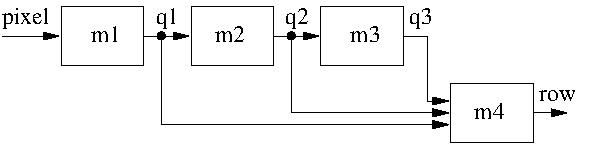
\includegraphics{ex3wf}
        \caption{A 3 pixel window}
        \label{fig:ex3wf}
        \end{figure}
        This is not the best way to implement a window operator.
        
        Firstly module m4 would have to be written so that is first accepted
        q1 only, then q1 with q2 and finally all three queue inputs. If m4
        waits on its 3 inputs it will read the same datum from all 3 and it
        will only output every 3 cycles, the pipeline being delayed 2 cycles
        in every 3. m2 and m3 must hold exactly one datum each, otherwise the
        window will not contain contiguous data. We could get around the
        startup problem by giving queues q2 and p3 initial data.
        
        Secondly these modules as shown would only be unit delays for which
        the queue overheads would be inefficient.
        
        It is far better to implement the window delays as static variables
        within a module.
        \begin{lstlisting}[gobble=8, language=threepl]
           module
           win3 (queue(out, "[3]uint:8") <- queue(in, "uint:8")) {
               static(del, "[2]uint:8");
               
               sync {
                   del[0] <- in;
                   del[1] <- del[0];
                   out[0] <<- in;
                   out[1] <<- del[0];
                   out[2] <<- del[1];
               }
           }        
        \end{lstlisting}
        Note that we needed a {\bf sync} block to bind the execution of the
        queue and static assignments to the availability of queues {\bf in} and
        {\bf out}. With a {\bf par} the two static assignments would have
        executed straight away regardless of the availability of the queues.

        We could parameterise this in a number of ways. Firstly we could make
        the window width a parameter -
        \begin{lstlisting}[gobble=8, language=threepl]
           module
           win1D (queue(out, "["+width+"]uint:8") <- queue(in, "uint:8"), int(width)) {
               static(del, "["+(width-1)+"]uint:8");
               
               sync {
                   del[0] <- in;
                   for (int(i, 1) ; i<(width-1) ; i++)
                       del[i] <- del[i-1];
                   out[0] <<- in;
                   for (int(i, 1) ; i<width ; i++)
                       out[i] <<- del[i-1];
               }
           }        
        \end{lstlisting}
        The above code could be written more simply as -
        \begin{lstlisting}[gobble=8, language=threepl]
           module
           win1D (queue(out, "["+width+"]uint:8") <- queue(in, "uint:8"), int(width)) {
               static(del, "["+(width-1)+"]uint:8");
               
               sync {
                   del[0] <- in;
                   del[1..width-1] <- del[0..width-2];
                   out[0] <<- in;
                   out[1..width-1] <<- del[0..width-2];
               }
           }        
        \end{lstlisting}
        Because input parameters are created and matched with arguments before
        output parameters we can use an immediate input parameter value as a
        dimension for an output parameter. An alternative would have been to
        simply omit any type for the output parameter and let the output
        argument (which must after all be correct) supply the parameter
        dimension.
        \begin{lstlisting}[gobble=8, language=threepl]
           module
           win3 (queue(out) <- queue(in, "uint:8"), int(width)) {
               .
               .
               .
           }        
        \end{lstlisting}
        
        
        We could now make the window module independent of data type, picking
        up the input and output types from the arguments -
        \begin{lstlisting}[gobble=8, language=threepl]
           module
           win1D (queue(out) <- queue(in), int(width)) {
               static(del, "["+(width-1)+"]"+type(in));
               
               sync {
                   del[0] <- in;
                   del[1..width-1] <- del[0..width-2];
                   out[0] <<- in;
                   out[1..width-1] <<- del[0..width-2];
               }
           }        
        \end{lstlisting}
        
        We could simplify this further by making the static the same type as
        the output queue, even though we need an array one smaller -
        \begin{lstlisting}[gobble=8, language=threepl]
           module
           win1D (queue(out) <- queue(in), int(width)) {
               static(del, type(out));
               
               .
               .
               .
           }        
        \end{lstlisting}
        Here we rely on code optimisation to remove the unused array member
        of static variable {\bf del}.
        
        The previous examples do not recognise frame boundaries.
        In practice we might have a frame input signal which is asserted
        during contiguous pixels in a frame and not asserted during frame
        gaps. To carry this signal along with the pixel data a struct would
        be used for the input stream -
        \begin{lstlisting}[gobble=8, language=threepl]
            struct(inpix,
                data,   "uint:8",
                frame,  "log"
            );
        \end{lstlisting}
        where {\bf frame} is true for valid pixels and false for data
        between frames. For the data output there would no longer be a gap
        in the data stream so we could perhaps flag the last window in a frame
        by using another struct -
        \begin{lstlisting}[gobble=8, language=threepl]
            struct(pixwin1,
                data,   "["+winwidth+"]uint:8",
                last,   "log"
            );
        \end{lstlisting}
        We have the choice of filling off-edge pixels in the 3-pixel window with
        a default value (0), adding another field to struct {\bf pixwin1} or
        else restricting the scan width to exclude off-edge pixels. The
        following example takes the second alternative. It is assumed that the
        gap between frames is wider than the window.
                          
        \begin{lstlisting}[gobble=8, language=threepl]
            int(winwidth, 3);
            queue(q1, inpix);
            queue(q2, pixwin1);

            win1D(q2 <- q1, winwidth);
            .
            .
            .

            module
            win1D (queue(out, pixwin1) <- queue(in, inpix), int(width)) {
                if (width%2 == 0)
                    texit("win1D - window width is not odd");
                else
                    int(centre, width / 2);
                static(del, "["+width+"]inpix");

                sync {
                    del[0] <- in;
                    del[1..width-1] <- del[0..width-2];
                    when (del[centre].frame) par {
                        for (int(i) ; i<width ; i++)
                            out.data[i] <<- del[i].data;
                        out.last <<- !del[centre-1].frame;
                    }
                }
            }        
        \end{lstlisting}
        Note that the {\bf sync} requires that both the input and output
        queues be available before the input queue will be read even when
        the window centre is off-edge. This is unlikely to be of concern.


    \section{a 2-dimensional pixel window}\label{sec:ex2Dw}

        We can extend on the previous example to make a 2D window.

        Since we are processing a 2D
        raster we can envisage an input signal that is asserted when a pixel is
        within a line and another that is asserted when a pixel is within a
        frame (frame now has a different meaning to that in the previous
        example). The input pixels will now have two fields in addition to the
        data -
        \begin{lstlisting}[gobble=8, language=threepl]
            struct(inpix,
                data,   "uint:8",   // pixel
                line,  "log",       // pixel within line
                frame,  "log"       // pixel within frame
            );
        \end{lstlisting}
        Here field {\bf line} will be true when a pixel is within a horizontal
        line and field {\bf frame} will be true when a pixel is within a frame.
        During line gaps {\bf line} will be false but {\bf frame} will remain
        true. Thus a pixel is valid when {\bf line} and {\bf frame} are both
        true.
        \begin{lstlisting}[gobble=8, language=threepl]
            struct(inpix,
                data,   "uint:8",   // pixel
                line,   "log",      // pixel within line
                frame,  "log"       // pixel within frame
            );
        \end{lstlisting}
        
        For a 2D array specification we can use a string -
        \begin{lstlisting}[gobble=8, language=threepl]
            int(winwidth, 3);
            str(pixarray, "["+winwidth+"]["+winwidth+"]");
        \end{lstlisting}
        which we can then insert in types -        
        \begin{lstlisting}[gobble=8, language=threepl]
            type(pixwin2D, pixarray+"inpix");
            struct(outpix,
                data,   pixarray+"uint:8",
                lastl,  "log",
                lastf,  "log"
            );
        \end{lstlisting}
        The output struct contains the 2D pixel array {\bf data}, a flag
        indicating that the central pixel is the last pixel in a line {\bf lastl}
        and flag indicating the last line in a frame, {\bf lastf}. {\bf lastf} will
        be true for every pixel window in the last line.



        
        
        \begin{lstlisting}[gobble=8, language=threepl]
            module
            win2D (queue(out, outpix) <- queue(in, inpix), int(linelen)) {
                int(ww, dimension(out.data, 0));    // window width
                if (ww%2 == 0)
                    texit("win2D - window width is not odd");
                else
                    int(centre, ww / 2);            // centre pixel of window
                static(del, pixwin2D);              // window - 2D array of pixels

                sync {
                    del[0][0] <- in;
                    del[1..ww-1][0] <- delay(del[0..ww-2][ww-1], linelen-ww-1,, true);
                    del[0..ww-1][1..ww-1] <- del[0..ww-1][0..ww-2];
                    when (del[centre][centre].line) sync {
                        for (int(i) ; i<ww ; i++)
                            for (int(j) ; j<ww ; j++)
                                out.data[i][j] <<- del[i][j].data;
                        out.lastl <<- !del[centre-1][centre-1].line;
                        out.lastf <<- !del[centre-1][centre-1].frame;
                    }
                }
            }
        \end{lstlisting}
        
        The \verb'..' construction indicates a subscript range. The code above
        connects up the window elements such that each row shifts one left and
        the the input for each row is the leftmost pixel of the previous row
        delayed by the line length - the widow length - 1. If expanded
        explicitly the above would look like -
        \begin{lstlisting}[gobble=8, language=threepl]
            int(ed, linelen-ww-1);  // extra delay - line length - window length - 1

            del[0][0] <- in;                    // input to 1st line

            del[1][0] <- delay(del[0][2], ed);  // 2nd line from end of 1st
            del[2][0] <- delay(del[1][2], ed);  // 3rd line from end of 2nd

            del[0][1] <- del[0][0]; // shift 1st line left
            del[0][2] <- del[0][1]; //   "    "   "    "
            del[1][1] <- del[1][0]; // shift 2nd line left
            del[1][2] <- del[1][1]; //   "    "   "    "
            del[2][1] <- del[2][0]; // shift 3rd line left
            del[2][2] <- del[2][1]; //   "    "   "    "
        \end{lstlisting}
        The library function {\bf delay()} implements a fixed delay. The 1st
        argument is the input. The 2nd argument is the delay line length. The
        3rd argument, if true, specifies that block RAM is to be used to contain
        the data rather than flip-flops or CLB shift registers. This should be
        specified where too many shift registers would be required otherwise.
        
        


    \section{pixel window operations}
    
        To carry out window operations on an image it is necessary to stream the
        image in some useful pixel order. This is not a limitation of 3PL,
        which can access arrays in parallel, but rather a limitation of the
        hardware on which 3PL target code executes. Because of the size of
        image arrays current FPGA-based processing boards can only store
        images in conventional RAM. To access the image it must be read
        through a port, usually one pixel at a time. To create a small window
        which scans through the image the image stream is delayed through
        successive line delay elements and pixel delay elements to form
        a parallel pixel window. Thus an {\bf n x n} window will require
        {\bf n-1} line delays and {\bf n x (n-1)} pixel delays. A pixel delay
        is simply a register but a line delay requires a small FPGA block RAM
        (rmemory). These blocks constitute the main limitation to the number
        and size of window operations we can perform in an FPGA. Of course
        if we can carry out a number of parallel operations on the same
        window we avoid proliferation of these delay elements.

        Using the above pixel window code we can perform the usual image processing
        array operations, for example a Sobel operator could be coded as -
        \begin{lstlisting}[gobble=8, language=threepl]
           int(iwidth, 1024);
           queue({pixel, sob}, "uint:8");
           queue(window, "[3][3]uint:8");
           
           .
           win3x3(window <- pixel, iwidth);
           sobel(sob <- window);
           .
           
           module
           sobel (queue(out) <- queue(in)) {
               value({s1, s2, s3, s4}, "int:10");
               value({m1, m2}, "int:11");
               
               s1 := in[0][0] + 2 * in[1][0] + in[2][0];
               s2 := in[0][2] + 2 * in[1][2] + in[2][2];
               s3 := in[0][0] + 2 * in[0][1] + in[0][2];
               s4 := in[2][0] + 2 * in[2][1] + in[2][2];
               m1 := s2 - s1;
               m2 := s4 - s3;
               out <<- (m1 > 0 ? m1 : -m1) + (m2 > 0 ? m2 : -m2);
           }
        \end{lstlisting}
        Further window operations would require more stages in the pipeline
        of calls to module {\bf pixwin()} and window operator modules.
        
        Note that the above sobel module is correct but it generates large
        combinatorial expressions whose logic depth is likely to prove a problem
        at high clock rates. We could recode it to use internal pipelining
        within the module -
        \begin{lstlisting}[gobble=8, language=threepl]
           module
           sobel (queue(out) <- queue(in)) {
               queue({s1, s2, s3, s4}, "int:10");
               queue({m1, m2}, "int:11");
               
               sync {
                   s1 <<- in[0][0] + 2 * in[1][0] + in[2][0];
                   s2 <<- in[0][2] + 2 * in[1][2] + in[2][2];
                   s3 <<- in[0][0] + 2 * in[0][1] + in[0][2];
                   s4 <<- in[2][0] + 2 * in[2][1] + in[2][2];
               }
               m1 <<- s2 - s1;
               m2 <<- s4 - s3;
               out <<- (m1 > 0 ? m1 : -m1) + (m2 > 0 ? m2 : -m2);
           }
        \end{lstlisting}
        Note that there is a {\bf sync} around the four queue assignment
        statements that read queue {\bf in}. This is not necessary for
        synchronisation since the internal queues {\bf s1} to {\bf s4} can
        only become unavailable simultaneously due to the symmetry of the code
        and hence these four assignments will execute simultaneously as they
        have a common input queue. However, the use of the {\bf sync} means
        that queue availability is only tested once after which the four
        assignments execute without further queue testing. If the {\bf sync}
        were omitted then each assignment would individually test queue
        availability before executing. This would result in duplicated logic,
        but it is not obvious if this would be give larger or smaller
        signal delays (code duplication can give smaller signal delays by
        keeping signal lines short and local).
        


    \section{traversing a memory}\label{sec:traverse}

        The following module traverses a memory from an address supplied
        as an argument (a queue), summing the
        contents until a zero entry is encountered, at which time the sum
        is output. We need to write the code differently depending on whether
        we use combinatorial output memory or registered output memory.
        
        For combinatorial output memory the read occurs within the current
        clock cycle so the data can be used directly. For this reason the
        combinatorial output memory read is a function rather than a
        procedure.
        \begin{lstlisting}[gobble=8, language=threepl]
           cmemory(mem, 1, "uint:8", "uint:8");

           module
           sum (queue(out, "uint:16") <- queue(inaddr, "uint:8")) {
               static(searching, "log");
               static(addr, "uint:8");
               static(sum, "uint:16");
               value(mrv, "uint:8", cmemoryread(mem, 0, addr));

               when (searching)
                   when ((mrv == 0)) sync {
                       reset(searching, sum);
                       out <<- sum;
                   } else par {
                       sum <- sum + mrv;
                       addr++;
                   }
               else sync {
                   sum <- cmemoryread(mem, 0, inaddr);
                   addr <- inaddr + 1;
                   searching <- true;
               }
           }
        \end{lstlisting}
        Initially {\bf searching} is false (by default) so the {\bf else} of the
        outer {\bf when} will be executed. This is a {\bf sync} which will wait
        for the starting address queue {\bf inaddr} to be available. When {\bf
        inaddr} is available the memory location whose address in {\bf in} will
        be read and assigned to the sum {\bf sum} and logical static {\bf
        searching} will be assigned {\bf true}. The search address {\bf addr}
        will be assigned {\bf in + 1} ready to continue the scan.
        
        The {\bf sync} starting the outer {\bf else} block is not strictly
        necessary as there is only one queue to be waited on and both dependent
        statements will hence execute at the same time. Also it does not matter
        if the assignment to {\bf searching} occurs in a separate clock cycle to
        the queue reads. The use of {\bf sync} there however will save checking
        the availability of {\bf inaddr} on two deparate statements.
        
        Note that for combinatorial output memory the output always reflects the
        current address input so despite the function name there is no explicit
        read.

        The outer {\bf when} will repeat in its implied infinite loop and this
        time will execute the true body. We want to do the memory read and then
        decide what action to take. By assigning the memory read function to a
        value variable, {\bf mrv} (memory read value), we can use the result in
        two places, the inner {\bf when} test expression and then optionally
        adding the value to the sum. It is important that the memory read and
        the address increment occur in the same clock cycle in the {\bf par}
        block, but there is no problem there as no queues are involved so there
        will be no queue waits.
        
        When {\bf searching} is true and {\bf mrv} is zero the sum can be
        written to queue {\bf out}. Since {\bf sum} is zeroed (along with searching)
        in the same parallel block as it is written to queue {\bf out} the block
        must be a {\bf sync} otherwise the sum will be zeroed whie waiting for
        the output queue to be available should it not already be so.    

        Note that the memory scan proceeds even if the output queue is not
        available right up until it is time to write the result to the output
        queue at which point there might be a wait on output queue availability.
        
        The nested when statements in the code above could be eliminated
        by detecting the three distinct states -
        \begin{lstlisting}[gobble=8, language=threepl]
           cmemory(mem, 1, "uint:8", "uint:8");

           module
           sum (queue(out, "uint:8") <- queue(inaddr, "uint:8")) {
               static(searching, "log");
               static(addr, "uint:8");
               static(sum, "uint:16");
               value(mrv, "uint:8", cmemoryread(mem, 0, addr));
               value(ieq0, "log", mrv == 0);

               sync {
                   when (searching && ieq0) sync {
                       reset(searching, sum);
                       out <<- sum;
                   }
                   when (searching && !ieq0) par {
                       sum <- sum + mrv;
                       addr++;
                   }
                   when (!searching) sync {
                       sum <- cmemoryread(mem, 0, inaddr);
                       addr <- in + 1;
                       searching <- true;
                   }
               }
           }
        \end{lstlisting}
        The sync will execute in an implied infinite loop as usual. The three
        {\bf when} statements will execute simultaneously within the {\bf sync}
        but the conditional expressions are mutually exclusive so that only one
        of them will execute its code block. The surrounding {\bf sync} locks
        them together, otherwise if one were waiting on a queue wait another may
        find that its conditional expression has changed and then it might begin
        execution at the same time. The {\bf sync} ensures that only one can execute
        at a time, given that their conditional expressions are mutually
        exclusive at the time of entry to the {\bf sync}. We could also
        achieve the same by using individual {\bf sync} statements -
        \begin{lstlisting}[gobble=8, language=threepl]
           cmemory(mem, 1, "uint:8", "uint:8");

           module
           sum (queue(out, "uint:8") <- queue(inaddr, "uint:8")) {
               static(searching, "log");
               static(addr, "uint:8");
               static(sum, "uint:16");
               value(mrv, "uint:8", cmemoryread(mem, 0, addr));
               value(ieq0, "log", mrv == 0);

               when (searching && ieq0) sync {
                   reset(searching);
                   out <<- sum;
               }
               when (searching && !ieq0) sync {
                   sum <- sum + mrv;
                   addr++;
               }
               when (!searching) sync {
                   sum <- cmemoryread(mem, 0, inaddr);
                   addr <- inaddr + 1;
                   searching <- true;
               }
           }
        \end{lstlisting}

        For registered output memory the output becomes available in the cycle
        following a read, the read being explicit.
        \begin{lstlisting}[gobble=8, language=threepl]
           rmemory(mem, 1, "uint:8", "uint:8");

           module
           sum (queue(out, "uint:8") <- queue(inaddr, "uint:8")) {
               static(searching, "log");
               static(addr, "uint:8");
               static(sum, "uint:16");
               value(mrv, "uint:8", rmemoryout(mem, 0));
               value(ieq0, "log", mrv == 0);

               when (searching && ieq0) sync {
                   reset(searching);
                   out <<- sum;
               }
               when (searching && !ieq0) sync {
                   sum <- sum + mrv;
                   rmemoryread(mem, 0, addr);
                   addr++;
               }
               when (!searching) sync {
                   rmemoryread(mem, 0, inaddr);
                   reset(sum);
                   addr <- inaddr + 1;
                   searching <- true;
               }
           }
        \end{lstlisting}
        This executes much as the previous example but will execute one extra
        memory read, which will not be used. The variable {\bf mrv} now
        represents the value of the memory output register holding the result of
        a memory read on a previous cycle.
        
        On the first memory read the result is not available until the next
        clock cycle. On the following clock cycle the previous read result
        is added to {\bf sum}, another memeory read is executed and the address
        is incremented, all in parallel.
        
        We could code the solution differently as follows
        \begin{lstlisting}[gobble=8, language=threepl]
           rmemory(mem, 1, "uint:8", "uint:8");

           module
           sum (queue(out, "uint:8") <- queue(inaddr, "uint:8")) {
               static(addr, "uint:8");
               static(sum, "uint:16");
               value(mrv, "uint:8", rmemoryout(mem, 0));

               seq {
                   sync {
                       rmemoryread(mem, 0, inaddr);
                       addr <- inaddr + 1;
                       sum <- 0;
                   }
                   while (mrv != 0) par {
                       rmemoryread(mem, 0, addr);
                       sum <- sum + mrv;
                       addr++;
                   }
                   out <<- sum;
               }
           }
        \end{lstlisting}
        This is an endlessly repeating sequence of three
        parts. The first reads the memory location given by the
        input queue {\bf inaddr}. This will wait until the input queue
        is available. Following this a {\bf while} loop continues
        until it encounters a zero entry, summing the values
        as it goes. The final part writes out the sum to the
        output queue (possibly waiting on its availability).
        This solution is more readable.
        
        The three examples above might be shortened by overlapping
        the output assignment with the next address input.



    \section{searching a linked list in memory}\label{sec:link}

        This illustrates linked list traversal using static
        variables. The memory contains items structured as link
        plus data. The queue function is passed an initial
        memory address. It follows links in the memory until it
        finds a zero address. At that point it outputs the
        associated data item.
        \begin{lstlisting}[gobble=8, language=threepl]
           str(type, "uint:8");
           struct(item,
               data,  type,
               addr,  type
           );
           rmemory(mem, 1, type, item);
           
           module
           find (queue(out, type) <- queue(inaddr, type)) {
               static(searching, "log");
               value(mrv, item, rmemoryout(mem, 0));

               if (!searching) par {
                   rmemoryread(mem, 0, inaddr);
                   searching <- true;
               } else par {
                   if (mrv.addr == 0) par {
                       reset(searching);
                       out <<- mrv.data;
                   } else
                       rmemoryread(mem, 0, mrv.addr);
               }
           }
        \end{lstlisting}

        As in the previous section we could write instead -
        \begin{lstlisting}[gobble=8, language=threepl]
           str(type, "uint:8");
           struct(item,
               data,  type,
               addr,  type
           );
           rmemory(mem, 1, type, item);

           module
           find (queue(out, type) <- queue(in, type)) {
               static(i, item);

               seq {
                   rmemoryread(mem, 0, in);
                   while (i.addr != 0)
                       rmemoryread(mem, 0, i.addr);
                   out <<- i.data;
               }
           }
        \end{lstlisting}



    \section{function generation using look-up tables}\label{sec:fglut}

        Arbitrary function generation can be performed by means of a
        look-up table. For example to generate a stream of sin values
        to a queue -
        \begin{lstlisting}[gobble=8, language=threepl]
            var(mi, "[256]uint");
            for (int(i) ; i<256 ; i++)
                mi[i] = 2048 + floor(2047.0 * sin(2 * i * math_pi / 256.0));

            rmemory(m, 1, "uint:8", "uint:12", mi);

            static(addr, "uint:8");
            queue(sinstream, "uint:12", depth=16);

            sync {
                rmemoryread(m, 0, addr);
                sinstream <<- rmemoryout(m, 0);
                addr++;
            }
        \end{lstlisting}
        The sin values are generated by immediate code and used as an
        initialisation array for the block RAM (rmemory). The 12 bit values are
        offset by 2048 so that they are positive. The rmemory has an 8 bit
        address to hold 256 values and the stored values are 12 bit unsigned.

        The following code takes the sin stream and drives an external MCP4822
        DAC to produce an analog sin wave. The data stream to the DAC is much
        slower than the sin generation which just waits, generating values when
        the queue {\bf sinstream} is not full.
        
        \begin{lstlisting}[gobble=8, language=threepl]
            module "spi.3pl"

            useclock(c32);  // 32MHz clock domain

            // sin generation code inserted here

            static({_cs, _ldac}, "log", true);
            static({sdi, sck}, "log");
            struct(s,
                val,        "uint:12",
                active,     "log",
                gain_low,   "log",
                dummy,      "log",
                select,     "uint:1"
            );
            queue(data, s);

            output(,, _cs, loc=C_pins[0]);  // DAC chip select
            output(,, sdi, loc=C_pins[1]);  // DAC serial data in
            output(,, sck, loc=C_pins[2]);  // DAC serial clock
            output(,, _ldac, loc=C_pins[3]);// DAC load value

            seq {
                sync {
                    data.select <<- 0;  // select A output
                    data.gain_low <<- true; // X1 gain
                    data.active <<- true;   // active
                    data.val <<- sinstream; // DAC value
                }
                _ldac <- false;
                _ldac <- true;
                wait(781.241e-6);       // delay for 5Hz 256 sample/cycle sin
            }

            value(spi_step, "log");     // SPI serial transmission step - 4MHz 32 / 8)
            seq {
                assert(spi_step <- );   // 1 cycle
                nop(7);                 // wait 7 cycles
            }

            spi_master(sck, sdi, _cs <- data,, spi_step);
        \end{lstlisting}
        
        This can be expanded to multi-phase by interleaved reads of the sin
        table since the table reads are very much faster in this case than
        the data transmitted to the DAC. Multiple DACs can be driven in parallel.









    \section{signal processing}\label{sec:dsp}
    
        It is not usually appropriate to use queue mode variables for
        signal processing pipelines. Queue mode variables are queues
        whereas what is required is a chain of registers. In a processing
        pipeline where queue mode variables are used each datum moves along
        the pipeline at clock rate regardless of other data. If input
        data is unavailable the pipeline empties from the input end.
        If the output is blocked then data fill the pipeline and become
        queued. A signal processing pipeline is implemented using a chain
        of registers where data is available on every clock cycle and the
        output is never blocked. Each register in the pipeline contains one
        datum. The data move in lock step every clock cycle.

        A signal processing schematic is shown in
        \autorefph{fig:dspex1}.
        \begin{figure}[htbp]
        \centering
        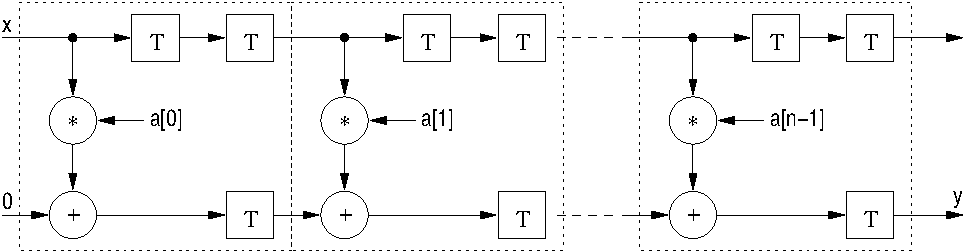
\includegraphics{dspex1}
        \caption{Simple signal processing example}
        \label{fig:dspex1}
        \end{figure}

        The code for a single stage might be -
        \begin{lstlisting}[gobble=8, language=threepl]
           module
           section (
               static({out0, out1}, "fixed:12.6")
               <-
               value({in0, in1}, "fixed:12.6"), float(a)
           ) {
               static(s, "fixed:12.6");
               
               s <- in0;
               out0 <- s;
               out1 <- a * in0 + in1;
           }
        \end{lstlisting}
        For simplicity and generality the input and output parameter types can
        be omitted, in which case the types of the arguments will be used -
        \begin{lstlisting}[gobble=8, language=threepl]
           module
           section (static({out0, out1}) <- value({in0, in1}), float(a)) {
               static(s, type(in0));
               
               s <- in0;
               out0 <- s;
               out1 <- a * in0 + in1;
           }
        \end{lstlisting}
        
        The complete filter could be constructed by -
        
        \begin{lstlisting}[gobble=8, language=threepl]
           int(n, 50);
           var(x_pins, "["+n+"]string", {"A2", "B4", ......}); // FPGA input pins
           var(y_pins, "["+n+"]string", {.........});          // FPGA output pins
           var(a, "["+n+"]float", {3.1, 2.7, ..........});     // coefficients
           input(x, "fixed:12.6", loc=x_pins);
           value(v1, "fixed:12.6", i1);
           value(v2, "fixed:12.6", 0);
           
           for (int(i) ; i<n ; i++) {
               section(v1, v2 <- v1, v2, a[i]);
           }
           
           output(,, v2, loc=y_pins);
        \end{lstlisting}
        Note the use of value variables {\bf v1} and {\bf v2} as both input
        and output arguments to the module {\bf section}. On each call the
        prior value of each variable is used and on each return these
        variables point to the new output parameter static variables. Thus
        {\bf v1} and {\bf v2} act as links between successive calls to construct the
        processing pipeline chain.

        A less regular example is shown in
        \autorefph{fig:dspex2}.
        \begin{figure}[htbp]
        \centering
        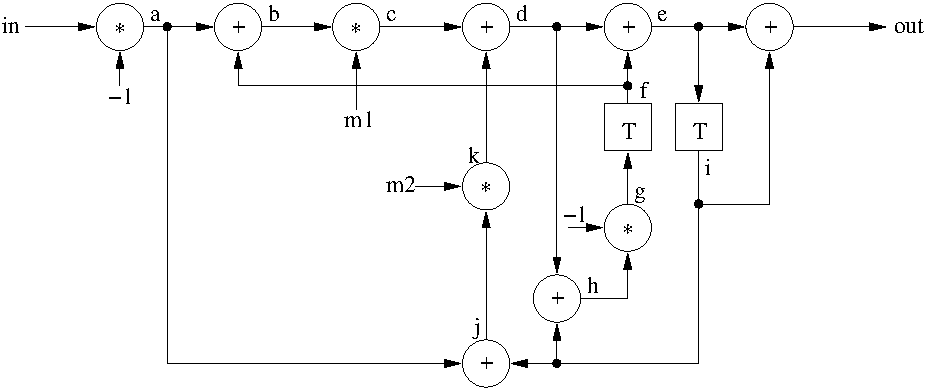
\includegraphics{dspex2}
        \caption{Complicated signal processing example}
        \label{fig:dspex2}
        \end{figure}
        This example is an IIR, or recursive, filter from
        a text on digital filters. The
        code for this is -
        \begin{lstlisting}[gobble=8, language=threepl]
           module filter (queue(in, "uint:16") <- queue(out, "uint:16")) {
               static({f, i}, "uint:16");
               value({a, b, c, d, e, g, h, j, k}, "uint:16");
               int(m1, ...);
               int(m2, ...);

               sync {
                   f <- g;
                   i <- e;

                   a := -in;
                   b := a + f;
                   c := b * m1;
                   d := c + k;
                   e := d + f;
                   g := -h;
                   h := i + d;
                   j := a + i;
                   k := j * m2;

                   out <<- e + i;
               }
           }
        \end{lstlisting}
        This could be shortened to -
        \begin{lstlisting}[gobble=8, language=threepl]
           module filter (queue(in, "uint:16") <- queue(out, "uint:16")) {
               static({f, i}, "uint:16");
               value({d, e, g}, "uint:16");
               int(m1, ...);
               int(m2, ...);

               sync {
                   f <- g;
                   i <- e;

                   d := (f - in) * m1 + (i - in) * m2;
                   e := d + f;
                   g := d - i;

                   out <<- e + i;
               }
           }
        \end{lstlisting}


    \section{A batcher parallel sorting network}\label{sec:batcher}

        A batcher sort network is generated by an
        algorithm, which must be written as immediate code. The following
        module creates a batcher sorting network for any number of inputs
        greater than 2. The input and output queues must be arrays of the same
        size and type {\bf uint} or {\bf int}.
        \begin{lstlisting}[gobble=8, language=threepl]
           module
           sort (queue(out) <- queue(in)) {
               int(inputs, dimension(in));
               int(stages, get_stages(inputs));
               int(sbits);     // bits to hold 'size'
               int(size2);     // power of 2 containing window size
               int(i);
               int({p, q, r}); // Batcher parameters
               int(d); // Batcher parameter - distance between exchange pairs
               int(wi);        // window member index
               int(si);        // network stage index
               var(ignore, "["+inputs+"]log"); // flags for skipping 2nd of exchange pair
               var(net, "["+(stages+1)+"]->");
               net[0] = &in;
               queuearray(net[1..stages-1] <- type(in));
               net[stages] = &out;

               for (i=inputs-1 ; i!=0 ; i=i>>1)
                   sbits++;
               size2 = 1 << (sbits - 1);

               for (p=size2 ; p>0 ; p=p>>1) {
                   r = 0;
                   d = p;
                   for (q=size2 ; q!=(p/2) ; q=q>>1) {
                       [
                           for (wi=0 ; wi<inputs ; wi++)
                               if (ignore[wi])        // already connected
                                   ignore[wi] = false;
                               else if ((wi < (inputs-d)) && ((wi & p) == r)) {// exchange
                                   cond_exchange ( net[si+1]->[wi], net[si+1]->[wi+d]
                                                   <-
                                                   net[si]->[wi], net[si]->[wi+d] );
                                   ignore[wi+d] = true;// ignore later
                               } else                  // straight through
                                   net[si+1]->[wi] <<- net[si]->[wi];
                       ]
                       d = q - p;
                       r = p;
                       si++;
                   }
               }
           }
        \end{lstlisting}
        Notice that the input and output queues are the only arguments passed
        to the module, all necessary parameters being derived from the
        characteristics of the input queue. The intermediate {\bf for} loop
        with loop variable {\bf q} generates an inline module on each
        iteration, each module handling one parallel stage of the sort. The
        stages are pipelined together. The inner loop generates conditional
        exchange assignments or direct assignments.
        
        The code needs an array of queues for the multi-stage network and since
        we cannot implement that directly a pointer array is used. The first
        and last pointers in the array are to the input and output queues. The
        intermediate pointers are to queues created by the library procedure
        {\bf queuearray()}.
        
        The immediate code which generates the target code uses
        Batcher's algorithm which will not be described here. The number of
        stages needed for the sort is determined by the following immediate
        function -
        \begin{lstlisting}[gobble=8, language=threepl]
           function
           get_stages (int(size)) {
               int({sbits, stages});

               for (int(i, size-1) ; i!=0 ; i=i>>1)
                   sbits++;
               for (stages=0 ; sbits>0 ; sbits--)
                   stages = stages + sbits;
               return(stages);
           }
        \end{lstlisting}
        Conditional exchanges are implemented by the following procedure -
        \begin{lstlisting}[gobble=8, language=threepl]
           procedure
           cond_exchange (queue(o0), queue(o1) <- queue(i0),  queue(i1)) {
               value(gt01, "log");

               gt01 := i0 > i1;
               par {
                   o0 <<- gt01 ? i1 : i0;
                   o1 <<- gt01 ? i0 : i1;
               }
           }
        \end{lstlisting}


\pagebreak

\chapter{Specific Limitations}

    \section{multiply, divide and remainder operators}
    
        \subsection{Virtex-E}

            In the Virtex-E there are no hardware multiply or
            divide functions. The multiply, divide and remainder operators
            carry out these operations using cascaded adders or subtractors.
            Since these are expression operators they cannot be pipelined. The
            result is that these operations have a large data delay, typically
            30ns to 40ns.
            
            \index{constraint!timing}
            \index{timing constraint}
            If the operation can be allowed to take place over several
            clock cycles between static variables then the timing constraints
            can be changed to suit, e.g.
            \begin{lstlisting}[gobble=12, language=threepl]
               static(a, "uint:8"); attribute(a, {tnm="SRC"});
               static(b, "uint:8"); attribute(b, {tnm="SRC"});
               static(c, "uint:16"); attribute(c, {tnm="DEST"});
               maxdelay("SRC", "DEST", 40.0e-9); // 40ns path constraint

               c <- a * b;     // slow operation!
            \end{lstlisting}
            
            If the operation must be at clock rate then pipelined 3PL library
            modules should be used for multiply, divide and remainder.
    
        \subsection{Virtex-II or Virtex-II Pro}

            In the Virtex-II or Virtex-II Pro there are hardware multipliers
            but no hardware dividers.

            The multiply operator uses one hardware multiplier for operands up
            to 18 bits if signed, 17 bits if unsigned. If one operand is between
            19 and 35 bits signed, or 18 to 34 bits unsigned, then two hardware
            multipliers plus an adder are used. If both operands are between 19
            and 35 bits signed, or 18 to 34 bits unsigned, then four hardware
            multipliers plus two adders are used.
            
            No attempt has been made to share hardware multipliers between
            products of small operands. Hardware multipliers are a limited
            resource and care must be taken not to exceed the number available
            in the particular FPGA being used.
                       
            There are no hardware dividers and divide and remainder operators
            carry out these operations using cascaded adders and subtractors.
            Since these are expression operators they cannot be pipelined. The
            result is that these operations have a large data delay, typically
            30ns to 40ns. For approaches to this see the previous subsection
            above (Virtex-E).
    
        \subsection{Virtex-5}

            In the Virtex-5 there are hardware multipliers but no hardware
            dividers. The multipliers are contained in the DSP48E blocks.

            The multiply operator uses one hardware multiplier for operands up
            to 25 bits by 18 bits signed. Unsigned operands have a 0 sign bit
            appended at the most significant end and thus become one bit
            larger.
            
            Selectvalue, static and queue mode variables which are assigned
            arithmetic or logical expressions can employ DSP blocks implicitly
            by setting the DSP attribute. In the case of static variables this
            will also use the DSP block output register rather than using
            flip-flops (but not if the variable is initialised to a value other
            than zero since the DSP block output register cannot be
            initialised). Selectvalue, static and queue mode variables can
            have the ALU attribute (and not the DSP attribute) in which case
            additions and subtractions in assigned expressions will be
            combined in a common ALU implemented in CLBs.
            
            To take advantage of the detailed architecture of the DSP blocks
            they can be instantiated directly by calling
            {\bf DSP48E()} \autorefph{sec:lpdsp48e} in library xc5v.3pl.
            Alternatively there are some useful modules providing a simpler
            interface in that library - \\
            adder/subtracter - {\bf dspaddsub} \autorefph{sec:lmdspaddsub} \\
            counter - {\bf dspcounter} \autorefph{sec:lmdspcounter} \\
            logical functions - {\bf dsplog} \autorefph{sec:lmdsplog} \\
            multiplier - {\bf dspmuladd} \autorefph{sec:lmdspmul} \\
            multiplier adder - {\bf dspmuladd} \autorefph{sec:lmdspmuladd} \\
            multiplier subtracter - {\bf dspmulsub} \autorefph{sec:lmdspmulsub} \\
            subtracter multiplier - {\bf dspsubmul} \autorefph{sec:lmdspsubmul} \\
            
            If these modules are used with no DSP48E registers then the
            blocks can be used as a combinatorial elements in simple
            static and queue variable assignments. If DSP48E internal
            pipeline registers are used then the pipeline delays must
            be taken into account. This complicates the programming style
            considerably and is a tradeoff for the performance and resource
            usage advantages gained.

    
        \subsection{Virtex-6}
        
            At the moment the support is identical to that for virtex-5 -
            see above.




    \section{registered output memory}
    
        Registered output memory in Xilinx FPGAs is block RAM. These are a
        limited resource.
    
        \subsection{XCV300E}
        
            Block RAMs in the XCV3 have 4,096 bits which
            can be configured as -
            
            \begin{tabular}{l l l}
            \hline
            data width & address width & depth \\
            \hline
            1  & 12 & 4096 \\
            2  & 11 & 2048 \\
            4  & 10 & 1024 \\
            8  & 9  & 512  \\
            16 & 8  & 256  \\
            \hline
            \end{tabular}

            i.e. anywhere from 8 bit address to 12 bit address.
            
            The 3PL compiler will select blocks of appropriate size
            and configuration to provide depths of 256 to 4096, using as
            many blocks as required to match the data width.
    
        \subsection{XCV3, XC2VP}
        
            Block RAMs in the XCV3 have 8,432 bits which
            can be configured as -
            
            \begin{tabular}{l l l}
            \hline
            data width & address width & depth \\
            \hline
            1  & 14 & 16384 \\
            2  & 13 & 8192  \\
            4  & 12 & 4096  \\
            9  & 11 & 2048  \\
            18 & 10 & 1024  \\
            36 & 9  & 512   \\
            \hline
            \end{tabular}

            i.e. anywhere from 9 bit address to 14 bit address
            (the unusual data widths result from the use of extra 'parity'
            bits at the wider configurations).
            
            The 3PL compiler will select blocks of appropriate size
            and configuration to provide depths of 512 to 16384, using as
            many blocks as required to match the data width.
    
        \subsection{Virtex-5, Virtex-6}
        
            Block RAM elements are grouped in pairs, each block containing
            18Kbits. The pair can be configured as a single 36Kbit block.
            18K blocks can be configured as - 
            
            \begin{tabular}{l l l}
            data width & address width & depth \\
            \hline
            1  & 14 & 16384 \\
            2  & 13 & 8192 \\
            4  & 12 & 4096 \\
            9  & 11 & 2048 \\
            18 & 10 & 1024 \\
            \end{tabular}

            36K blocks can be configured as - 
            
            \begin{tabular}{l l l}
            data width & address width & depth \\
            \hline
            1  & 15 & 32768 \\
            2  & 14 & 16384 \\
            4  & 13 & 8192  \\
            9  & 12 & 4096  \\
            18 & 11 & 2048  \\
            36 & 10 & 1024  \\
            \end{tabular}
            
            The 3PL compiler will select blocks of appropriate size and
            configuration to provide depths of 1024 to 32768, using as many
            blocks as required to match the data width.

            Block RAM is also used to implement deep queues. For queues whose
            depth is 512, 1024, 2048, 4096 or 8192 a FIFO primitive element is
            used. This uses a block RAM with inbuilt FIFO control logic, saving
            considerable external CLB logic and probably giving improved
            performance (but note that the clock to output time of nearly 2nS
            still persists). The hardware FIFO is not used in the case of
            asynchronous queues on which the queuereadstatus() and
            queuewritestatus() have been used.

    \section{selectvalue variables}

        Selectvalue variables implement buses using CLB logic unless explicitly
        directed to use 3-state buffers driving partitionable 'long lines'. This
        is done by setting attribute "threestate" on individual selectvalue
        variables. These are only available on older FPGAs such as
        Virtex-E, Virtex-II and Virtex-II Pro.
        

    \section{high speed serial}
    
    
        \subsection{Virtex-II Pro}
        
            MGT high speed serial ports are interfaced using library {\bf
            gt\_custom\_16()} \autorefph{sec:lmgtcustom16} in library {\bf
            xilinx/mgt.3pl}.
    
        \subsection{Virtex-5, Virtex-6}
        
            GTP high speed serial ports are interfaced using library
            module {\bf gtp\_dual\_16()} \autorefph{sec:lmgtpdual16} in
            library {\bf xilinx/gtp\_dual.3pl}.
            
            GTX high speed serial ports are not yet supported.


\pagebreak

\chapter{Using CPLDs}

    The Xilinx Coolrunner and XC9500 CPLDs are supported. The variable modes {\bf
    selectvalue}, {\bf queue}, {\bf cmemory} and {\bf rmemory} cannot be used.
    
    For {\bf static} mode variables the {\bf continuous} attribute is true by
    default. This means that top level static assignments will not have an
    initiated execution thread containing an infinite loop but instead the register
    clock enable will be continuously asserted.

    For {\bf output} mode variables the {\bf direct} attribute is true by default.
    This means that conditional (3-state) output will have the enable
    driven directly from the conditional test expression rather than from
    an initiated execution thread.
    
    Target multiplication, division, remainder and variable left or right shift
    are not implemented for CPLDs.
    
    The following 3PL program illustrates XC9500 usage -
    \begin{lstlisting}[gobble=4, language=threepl]
        part("XC9536PC44-5");

        module "xilinx/xc95.3pl";

        var(inpins, "[]str", {"P11", "P12", "P13", "P14", "P18", "P19", "P20"});
        str(outpin, "P22");
        var(countpins, "[]str", {"P34", "P35", "P36"});
        str(clkpin, "P5");

        clock(clk, frequency=1.0e6, loc=clkpin);

        useclock(clk);

        input(in, "[7]log", loc=inpins);

        static(o, "log");
        static(count, "uint:3", 5);
        output(,, count, loc=countpins);

        count++;

        seq {
            o <- in[0] && in[1] && in[2] && in[3] && in[4] && in[5] && in[6];
            o <- false;
        }

        output(,, o, loc=outpin);
    \end{lstlisting}
    
\pagebreak

    For Coolrunner CPLDs the I/O standard can be specified -   
    \begin{lstlisting}[gobble=4, language=threepl]
        part("XC2C32APC44-6");

        module "xilinx/xc2c.3pl";

        var(inpins, "[]str", {"P25", "P26", "P27", "P28", "P29", "P33", "P34"});
        var(outpin, "str", "P35");
        var(clkpin, "str", "P5");

        clock(clk, frequency=1.0e6, loc=clkpin);

        useclock(clk);

        input(in, "[7]log", loc=inpins);

        static(o, "log");

        seq {
            o <- in[0] && in[1] && in[2] && in[3] && in[4] && in[5] && in[6];
            o <- false;
        }

        output(,, o, loc=outpin);
    \end{lstlisting}
    
    The 3PL compiler will run the appropriate Xilinx CPLD fitting software,
    if post-processing is not disabled.
    The final product is a JEDEC file with a {\bf .jed} file name extension.


\pagebreak

\chapter{Setting up an FPGA board}\label{chap:boardsetup}
    
    The Gadget Factory papilio board provides a good example of
    the way 3PL is set up for a specific board.
    
    The following is a very simple 3PL application program for the papilio -
    
    \begin{lstlisting}[gobble=8, language=threepl]
        module "boards/gadget_factory/papilio_one_500.3pl"

        static(t, "log");

        seq {
            wait(0.5);
            t <- !t;
        }

        output(,, t, loc=A_pins[0]);
    \end{lstlisting}
    
    This trivial program outputs a 1Hz square wave on connector A pin 0 (P18).
    The only requirement in setting up the platform is the first statement
    which imports a file module specific to the papilio one 500.
    A 32MHz clock is established by default and is the current clock domain.
    
    The imported file looks as follows -

    \begin{lstlisting}[gobble=8, language=threepl]
        nosource

        // 3pl board support for GadgetFactory Papilio One 500k board

        part("XC3S500EVQ100-4");

        module "xilinx/xc3s.3pl"

        // all IO is 3.3V on this board
        str(lvcmos33, "LVCMOS33");

        // clock generator 32MHz
        iopins(c32_pin, "str", "P89", frequency=32.0e6, ibufg=true, iostandard=lvcmos33);

        // 48 I/O pins across A (wing 1A), B (wing 1B), C (wing 2A)
        iopins(global.A_pins, "[16]str", {
	        "P18", "P23", "P26", "P33", "P35", "P40", "P53", "P57",
	        "P60", "P62", "P65", "P67", "P70", "P79", "P84", "P86"
            }, iostandard=lvcmos33
        );
        iopins(global.B_pins, "[16]str", {
        .
        .
        .
        .

        iopins(global.flash_cs_pin, "str", "P24", iostandard=lvcmos33);
        iopins(global.flash_clk_pin, "str", "P50", iostandard=lvcmos33);
        iopins(global.flash_mosi_pin, "str", "P27", iostandard=lvcmos33);
        iopins(global.flash_miso_pin, "str", "P44", iostandard=lvcmos33);

        // FTDI USB channel B serial receive and transmit
        // Labelling is reversed to schematic!
        // 'tx' should be an FPGA output, 'rx' an input
        iopins(global.serial_rxd_pin, "str", "P88", iostandard=lvcmos33);
        iopins(global.serial_txd_pin, "str", "P90", iostandard=lvcmos33);

        // create 32MHz clock
        clock(c32_in, loc=c32_pin);
        simpleclock(global.c32, c32_in);
        useclock(c32);

        directive("comms_baud_rate", 115200); // define default serial device baud rate
        module "xilinx/uart_cpu.3pl"


        trailermodule ("create uart bus interface") {
            create_bus_interfaces();
        }
    \end{lstlisting}
    Some of the pin definitions have been omitted ... to shorten the listing.
    
    This file module specifies parameters for this particular board.
    
    The call to inbuilt procedure part() specifies the Xilinx FPGA part number.
    
    The next statement imports the file module xilinx/xc3s.3pl, described later.
    That file module specifies parameters appropriate for the particular FPGA.
    
    The calls to iopins() build a map of all input and output FPGA pins and
    attributes associated with them, such as the FPGA pin name and the I/O
    standard. Additional attributes can be specified when the pins are
    passed to an input(), output() or clock() inbuilt procedure.
    
    The first call to iopins() specifies the clock input pin (P89), the clock
    frequency, (32MHz), specifies that an IBUFG should be used and that the I/O
    standard is LVCMOS.
    
    A call to clock() creates a clock mode variable, \verb'c32_in'. The call to
    simpleclock() in xilinx/clocks.3pl creates a global clock mode variable c32,
    a clock manager (DCM) and a clock buffer. c32 is then made the current clock.
    
    Module \verb'xilinx/uart_cpu()' is imported to provide a CPU interface
    to the FPGA using the serial link. That interface is set up at the end
    by a trailer module which calls \verb'create_bus_interfaces()'
    
    Finally a trailer module is created to call \verb'create_bus_interfaces()'
    after the source code exits to build the logic required to flesh out
    the CPU/FPGA interface. Calls to the interface routines are made throughout
    the source code and this logic is required at the end to tie it all
    together.
    
    
    
    
    
    
    
    
    The file module xilinx/xc3s.3pl, while specific to the Spartan 3S, also
    imports libraries relevant to all Xilinx FPGAs.
    
    \begin{lstlisting}[gobble=8, language=threepl]
        // Include file for Xilinx Spartan 3 (XC3S) elements
        nosource

        presetdirective("postProcessTool", "ise");  // ISE will be used

        source "xilinx/common.3pl"      // xilinx common library
        module "xilinx/postprocess.3pl" // code to run ISE or Vivado
        module "stdlib.3pl"             // standard 3PL generic library
        module "xilinx/clocks.3pl"      // xilinx clock managers
        module "xilinx/io.3pl"          // xilinx I/O facilities

        // Specify allowed special I/O and clock elements valid for
        // this device.
        // Map "elementMap" is in common.3pl.
        elementMap["BUFG"] = true;
        elementMap["BUFGMUX"] = true;
        elementMap["BUFGCTRL"] = true;
        elementMap["DCM"] = true;

        leadermodule ("attributes", 100) {
            attributeprocedure(processPinAttributes);
        }

        trailermodule ("constraints", 100) {
            netlistcommentfromdirs();
            generateConstraints();
        }

        postmodule ("Xilinx postprocessing") {
            postprocess("xilinx/ise_fpga.cmd", directive("postProcessTool"), 9.1);
        }
    \end{lstlisting}

    This sets a directive to select the place-and-route tools to be used ("ise"
    or "vivado") and imports several appropriate libraries that might be needed.
    
    A leader module, which is executed prior to other source code, calls
    inbuilt procedure attributeprocedure() to notify 3PL that the library
    procedure processPinAttributes() in xilinx/common.3pl is to be called
    whenever an input() output() or clock() inbuilt procedure is called
    with I/O pins. This procedure is called for each pin and processes associated
    attributes and constraints for the pin.
    
    A trailer module, which is executed after the source program exits, calls two
    procedures, netlistcommentfromdirs() in stdlib.3pl and generateConstraints()
    in xilinx/common.3pl. The first of these simply copies all directives and
    their values as comments to the netlist (EDIF) file . The second generates
    constraints from information gathered during immediate execution.

    Finally a post-processing module is created which calls postprocess() in
    xilinx/postprocess.3pl.  (Note that post processing by the Xilinx tools can
    be supressed by the -s option when running 3pl. This might be done if the
    tools are to be run manually or perhaps on another computer. For example if
    3pl is executed on Apple OSX the Xilinx tools have to be executed on a Linux
    or Windows emulator such as Virtualbox or else run on another computer since
    Xilinx do not support OSX).






\pagebreak

\chapter{Running the Compiler}
\label{chap:run3pl}


    The 3PL compiler is written in Java. It can be run on any computing
    platform that supports Java 1.6 or later. The 3PL compiler was developed
    and used in UNIX and MACOS environments, but can be run in a Windows
    environment as well.
    
    To use 3PL only the following are needed -
    \blist
    \item   the jar file - classes/3PL.jar
    \item   the 3PL libraries in sources/include
    \blend
    
    
    A script for running 3PL should be of the form -

    \verb'exec java -Xmx800M -jar .../3PL/classes/3pl.jar -I.../3PL/sources/include  $*'

    The first option of the Java call provides more heap space than default.
    The -I gives the location of the libraries.

    The compiler generates a Xilinx EDIF netlist file, some associated ISE or
    Vivado constraint files and three optional report files. It can then
    optionally run ISE or Vivado to produce a configuration file that can be
    executed on the FPGA (see below).
    

    \section{Environment variables}

        The environment variable {\bf THREEPL\_INCLUDE\_DIRS} gives an
        additional location of 3PL libraries. It is searched following the
        current directory and the directory specified by the command line -I
        option.

        3PL will by default attempt to post-process the configuration by
        executing the procedure postprocess() in xiline/postprocess.3pl,
        which runs the Xilinx ISE or Vivado tools. The post-processing module
        is described in \autorefph{ch:pp}.
        
        If manual invokation of place-and-route tools is prefered
        then the post-processing can be supressed by
        giving the -s option or by including the following in the 3PL
        source -
        \begin{lstlisting}[gobble=12, language=threepl]
            directive("skipPostProc", true)
        \end{lstlisting}
        
        If 3PL post-processing is to be used then the environment variable
        {\bf XILINX} must be set to the installation directory of the Xilinx
        post-processing tools, typically {\bf /opt/Xilinx} or similar. This
        directory would have been selected when the Xilinx tools (either ISE
        or Vivado) were installed. The standard Xilinx installation structure
        under this directory is assumed. It can be overridden by a 3PL
        directive of the same name.

        The following environment variables should not normally be defined by
        the user, but may be required in unusual situations -

        {\bf XILINX\_ISE}. Specifies a precise version of Xilinx ISE to use,
        for example  {\bf /opt/Xilinx/14.7i}. It can be overridden by a 3PL
        directive of the same name. This overrides the {\bf XILINX}
        environment variable, if defined. Normally the 3PL post-processing
        code will choose the newest version appropriate for the device.

        {\bf XILINX\_VIVADO}. Specifies a precise version of Xilinx Vivado to
        use, for example  {\bf /opt/Xilinx/Vivado/2019.1}. It can be
        overridden by a 3PL directive of the same name. This overrides the
        {\bf XILINX} environment variable, if defined. Normally the 3PL
        post-processing code will choose the newest version appropriate for
        the device.


    \section{Generating EDIF}
    
        The 3PL compiler is run by -
        \begin{verbatim}
        3pl {-Idirectories} {-dhlpst} name
        \end{verbatim}
        where the source file is "name.3pl" (the file name extension need not
        be given in the call to the compiler, though it is accepted). The
        file name argument may be a path containing "/"s.
        There must be only one source file argument.

	The {\em design name} is derived from the source file name argument by
	removing the trailing ".3pl" if present and removing the preceding
	file path up to the rightmost "/" if any.

	The design name may be set by a command line option {\bf -N name}.
	It may also be changed by calling inbuilt procedure
        {\bf designname()} where the string argument supplies a new design name.
        The command line option overrides the inbuilt procedure call which in
        turn prevails over the default derivation from the file name.
        
        The design name is also changed if inbuilt procedure {\bf export()} is
        called to create a logic core EDIF file.
	\index{constraint}
        
	The design name should comprise only alphanumeric characters or "\_"
	(underscore). Any other characters are silently converted to "\_".
	This is to ensure the design name matches the output file names and
	also observes EDIF identifier name restrictions. 

	The compiler will create a Xilinx EDIF netlist file called "name.edn"
	and either a Xilinx ISE constraint file, "name.ncf", or a Vivado
	constraint file, "name.xdc", where "name" is the design name.
        
        The {\bf -I} option specifies a ":"-separated list of directories
	to be searched for files to be included by {\bf source} and
	{\bf module} statements. There may be more than one {\bf -I} and they
	may precede or follow the source file name.
        The "-I" may be separated from its list by spaces, i.e. the list is
        the following argument. Directories are searched in the order -
        current directory, {\bf -I} option lists in order, then finally the
	3PL library directory.
	Therefore, source/module files may be preempted by including alternative
	versions earlier in the directory search path.
        
        To write the three output files to a directory other than the current
        directory a {\bf -o} option can be used. The directory name can
        be appended to the {\bf -o} or can be the following argument. The
        directory will be created if it does not exist.
        
        The call options are - \label{options}
        \blist
        \item   -c - compile only, do not execute
        \item   -d - display the interactive netlist schematic window after
                outputing an EDIF netlist
        \item   -D d=s - define a directive d whose value is string s
        \item   -f - force compilation even if sources have not been changed
        \item   -F - error messages use full path names rather than file names
        \item   -G - use gates rather than LUTs to help optimisation
        \item   -h - print a help message
        \item   -i - intermediate code only
        \item   -I d1:d2:.. - list of directories to search for libraries
        \item   -l - annotate printed TDE list with source file locations
        \item   -n - print a list of netlist net identifiers and their
                equivalent signal names to a file 'name'.net
        \item   -N name - change design name to 'name'
        \item   -o dir - write file to directory 'dir'
        \item   -p - print the TDE list prior to optimisation
        \item   -R - just print token generator output - testing only
        \item   -r - generate a verbose report to file 'name'.rpt
%        \item   -S - run the simulator instead of producing output code
        \item   -s - skip post-processing
        \item   -T - print the TDE list (including signal definitions)
        \item   -t - print the TDE list (excluding signal definitions)
        \item   -V - print the compiler version information 
	    		(with -v, prints more)
        \item   -x - suppress netlist code optimisation - testing only
        \item   -X - development mode - testing only
        \item   -Y - print clock domain resolutions (compiler diagnostic)
        \blend
        
        3PL will by default check the times of last modification of all referenced
        source and library files and the compiler make date. If all of these are older
        than the output netlist file and report file the compiler will exit without
        compiling and executing. This can be overridden by using the -f option to
        force compilation and execution.
        
        At the end of netlist generation 3PL will execute any post-processing
        modules. If this is not desired the -s option will cause this to
        be skipped.
        
        The -r option causes a detailed report to be produced in file {\em
        design\_name}.rpt.
        
        The -t option will result in a listing of the intermediate code in file
        {\em design\_name}.icl. The -l, -p and -T options modify the
        intermediate code listing and are only used for compiler testing.
        
        The -c option terminates 3PL after parsing the source file.
        
        The -i option terminates 3PL after immediate execution.
        
        The -R, -x, -X and -Y options are only used for compiler testing.
        
        The -D option defines a directive. The directive may be just a
        key, in which case a directive of type "log" with that key and value
        {\bf true} will be created. If key=value is given then the directive
        will be given the specified value and its type will be as appropriate
        for the value ("log", "int" or "float"). Space between the -D and the
        key is optional.
        
        The -G option replaces many LUTs normally produced by the code generated
        with nested gates. The logic remains the same but the use of nested
        gates instead of explicit LUTs may change the way the vendor
        place-and-route software optimises and packs the logic which in turn may
        change the ease, or lack thereof, with which the timing contraints can
        be met. Thus when timing constraints fail to be met trying the -G option
        may improve the situation. The same effect can be achieved by setting
        directive {\bf gatesNotLUTs} true prior to completion of immediate
        execution.

        -I, -o, -D and -N may each be, but need not be, separated from its
        argument by spaces.
        
        These options also set associated directives and for most of them
        the directives can also be set during immediate execution - see
        \autorefph{sec:directives}.
        
        If 3PL is called with no command line arguments, it pops up a GUI to
        open the file.
        
        \scalebox{0.5}{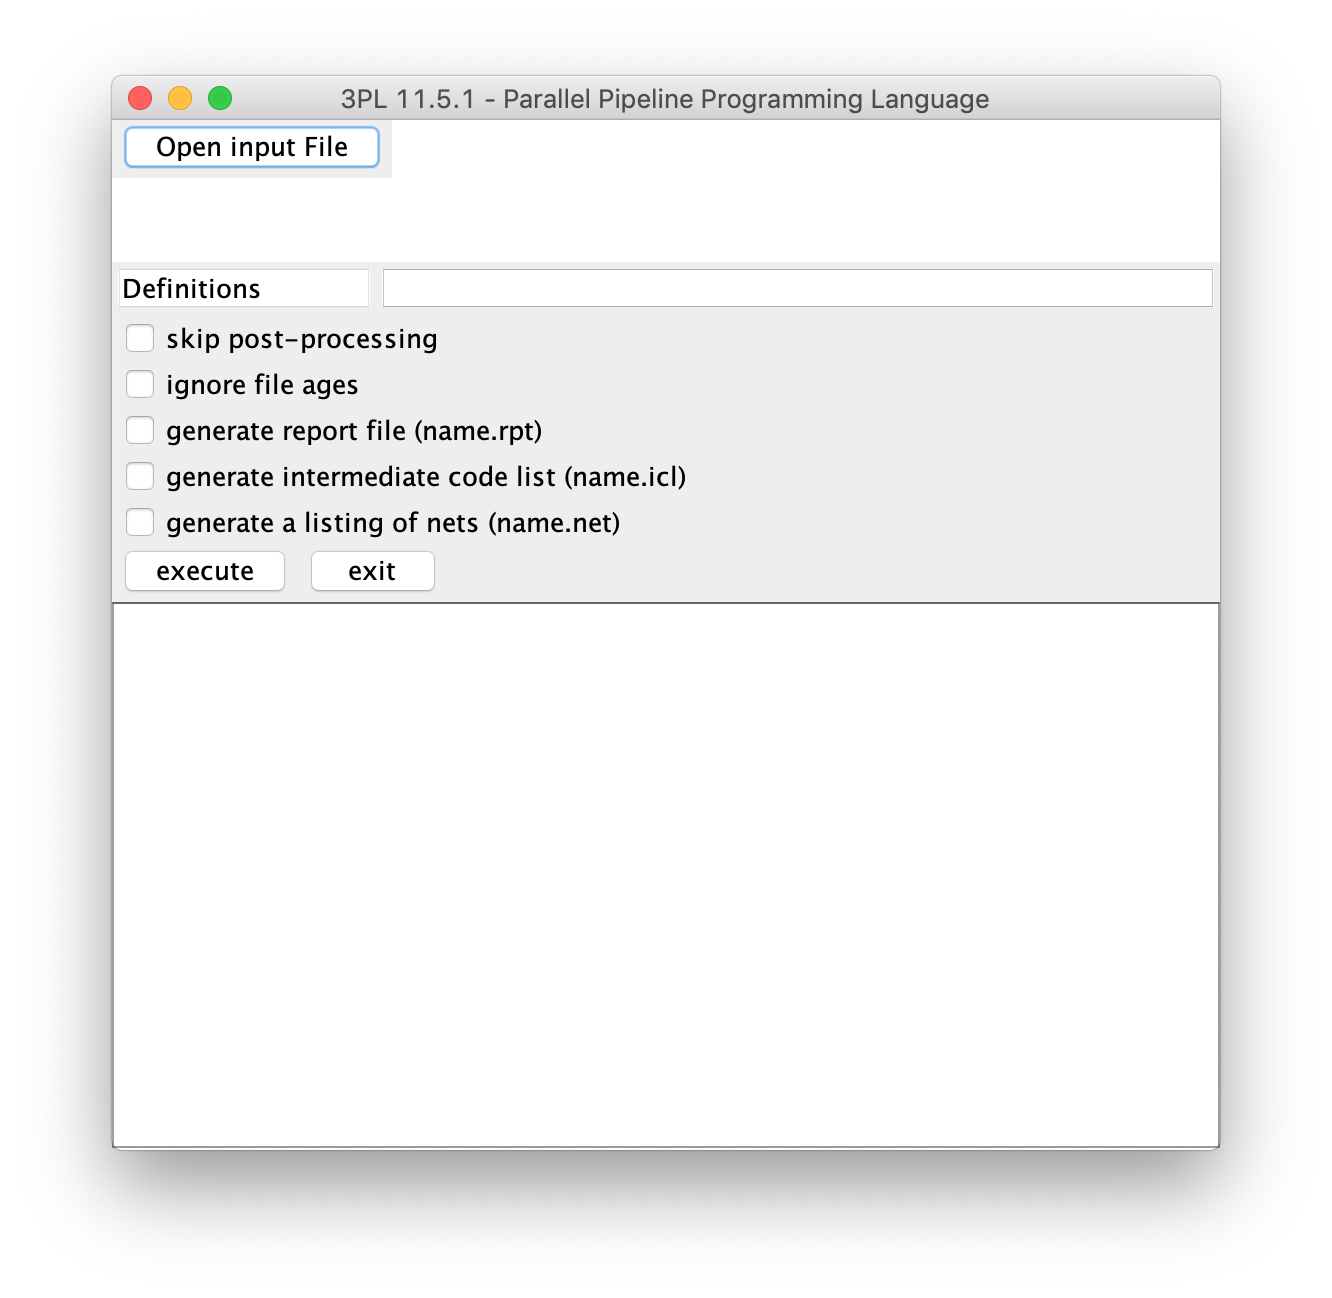
\includegraphics{3PL_GUI}}
        
        The GUI has text fields to specify the source file and any directives to
        define, buttons to set some options and a button to start (parsing,
        immediate execution and then code generation). The output appears in a
        scrollable text window. A file can be repeatedly compiled and executed
        by a single button press. Run this way it is still convenient to run via
        a script so that the library directory is specified and the Java memory
        heap maximum size is set. Directive definitions are space-separated and
        may be {\em name}=value or simply {\em name}. The value may be an
        integer, floating point or the strings "true" or "false". If none of
        those then it will be assumed to be a string value, any enclosing double
        quotes being removed. Where just a directive name is given it will be
        type "log" (boolean) with value TRUE. If the directives string is
        erroneous it will change colour to red.


        Unfortunately the 3PL compiler terminates immediately on most parsing
        errors. This means that you can only fix one error at a time. Making
        the compiler continue following a parsing error is something the author
        has not yet worked out how to accomplish with the compiler compiler
        that was used.

        The error messages have been designed to be as clear and informative as
        possible. However, the following parse error is an exception -
        \begin{verbatim}
        Parse error: file 'prog.3pl' line 2
        Encountered "#m#prog.3pl#2#\n in column 1.
        Was expecting one of:
            "break" ...
            "calling." ...
            "case" ...
            .
            .
            .
        \end{verbatim}
        This has resulted from unmatched braces around a module definition
        in a file included via a {\bf module} or {\bf source} statement!

        An immediate execution error causes termination, which is reasonable.
        
        If a post-processing module is provided then conditional code within
        it will carry out place-and-route and any other such tasks. This is
        described in the next section.
        

    \section{Generating Xilinx FPGA and CPLD configurations}\label{sec:xpp}
    
        See also \autorefph{ch:pp}

    	3PL post-processing code will by default run the Xilinx ISE or Vivado
	tools to transform the EDIF and constraint files generated by 3PL into
	configuration files that may be downloaded into the device for execution.
	To prevent this either the -s option or the "skipPostProc" directive must
        be set true. This might be done where 3PL is executed on a different
        host to that of the place-and-route tools or where the user prefers
        to run the place-and-route separately for some reason.

	The post-processing code automatically selects the Xilinx tool set and
	version based on the FPGA or CPLD part. Xilinx Vivado is used for 7-series
	FPGAs, and ISE for all other FPGAs and CPLDs.

	The code uses the newest installed version of ISE or Vivado, found under
	the installation directory specified by the {\bf XILINX} environment
	variable or 3PL directive, that supports the part.
	This is because Xilinx dropped support for older parts as newer
	versions of ISE were released, and older versions of the software did
	not support later parts.

	This version can be overridden if necessary using either the
	{\bf XILINX\_ISE} environment variable or 3PL directive, or the
	{\bf XILINX\_VIVADO} environment variable or 3PL directive, as
	appropriate. The need to do so should be rare.

	Actual post-processing uses a 'recipe' file. For ISE the recipe file is
	a simple list of ISE commands to run. The default recipe for FPGAs is 
	the file {\bf xilinx/ise\_fpga.cmd} -

        \begin{verbatim}
	ngdbuild @designName@
	map -detail -w -timing -ol high -pr b @designName@
	par -w -ol high @designName@ @designName@.ncd
	bitgen -m -w -g LCK_cycle:4 -g GTS_cycle:1 @designName@
        \end{verbatim}

	Items in the recipe file enclosed with \verb+@+ characters are replaced
	with the 3PL directive of the same name. Generally only the "designName"
	and "part" directives are useful.
	The ISE commands are executed in order, until one of them returns an
	error status or the script is completed.

%        where {\em xtimerr} is the script
%        \begin{verbatim}
%        \#! /usr/bin/sh -f
%        ggrep -q 'All constraints were met' $1.par
%        if ($status == 0) then
%            /bin/rm -f $1.twr $1.err
%        else
%            trce -e 50 -skew $1
%        endif
%        \end{verbatim}
%        \index{constraint!timing}
%        \index{timing constraint}
%        This conditional executes the Xilinx tool {\bf trce} if timing
%        constraints were not met during the place-and-route. This creates
%        a report file "name.twr"

	For Vivado the recipe file is a Tcl script run in the Vivado Tcl
	interpreter in non-project mode.
	The same \verb+@+-substitution is performed on the recipe first.
	The default recipe is {\bf xilinx/vivado.tcl} -

        \begin{verbatim}
	# read the EDIF netlist file into Vivado
	read_edif @designName@.edn

	# read the constraints file into Vivado (if there is one)
	if {[file exists @designName@.xdc]} {
	    read_xdc -ref @designName@ @designName@.xdc
	}

	# place and route the design
	link_design -top @designName@ -part @part@
	opt_design
	power_opt_design
	place_design
	phys_opt_design
	route_design
	phys_opt_design
	write_checkpoint -force @designName@.dcp

	# emit the reports
	report_timing_summary -file @designName@.tim
	report_io -file @designName@.pad
	report_utilization -file @designName@.xlxs
	report_clock_utilization -file @designName@.clku

	# write bitstream
	write_bitstream -force @designName@.bit
	\end{verbatim}

        Note that a checkpoint file is created so that it can be read into
	Vivado in GUI mode and the design layout can be examined.

	Both ISE and Vivado are run in the 3PL compiler output directory, as
	specified by the -o option. This means that the recipe files can expect
	their input netlist and constraint files in the 'current' directory,
	and the many output files from the ISE and Vivado programs are also
	written to the output directory.

	The default ISE and Vivado recipe files should be adequate for most
	3PL programs, but if necessary they can be overridden by defining the
	3PL directive "postProcessRecipe". This should be the filename of the
	recipe, not the recipe itself, and is searched for on the same
	include directory path as the 3PL {\bf source} and {\bf module}
	statements. It would typically be located within the user's source
	code.

	The voluminous output from the ISE and Vivado programs is filtered
	so that only warning and error messages are printed. This may be
	changed using the 3PL directive "postProcessFilter", which should have
	string values "error", "critical", "warning", "info", or "all".
	The 3PL compiler -v option (verbose) has the same effect as "all".
        
	If the 3PL directive "postProcessAppendFile" is defined and the file
	it names is readable, it is appended to the FPGA configuration file
	with a separator string. Board support modules use this to attach a
	text report or information file to the configuration. This can be
	examined to determine the provenance of the configuration.
	The extra data has been found not to upset FPGA configuration loaders,
	and it seems to be ignored. 

	If the 3PL boolean directive "postProcessCompress" is defined and true
	the FPGA configuration file is compressed using gzip.

    \section{The report file}
    
        The report file is produced when the -r option is provided on calling
        3PL. It has the following sections -
        
        {\bf \underline{Source files}}
        
            Source files are listed starting with the primary source file in the
            3PL call and then files inluded by {\bf module} or {\bf source}
            statements the order they are read. The list entries are indented
            to reflect the nesting depth of each included file.
            
            Each line has three components, a label, a directory path and the
            3PL source file in that directory.
            
            The label is "SRC" for a file included by a {\bf source} statement
            and is "FMODn", where 'n' is 1, 2, 3 etc. for a file included by
            a {\bf module} statement.
            
            Signal names are constructed using the file path as a prefix. This
            generates quite long signal identifiers. To reduce this the "FMODn"
            labels are used in place of directories. Thus unique signal names
            are still ensured but are shortened. When reading the intermediate
            code list the path string of a source file can be determined by
            consulting the source file list and matching the label.
        
        {\bf \underline{Leader modules main module and trailer modules}}
        
            Each leader module is listed as it is executed using the identifying
            string supplied in the source code. The ordering number is also
            listed.

            The main module is then executed

            Finally each trailer module is listed as it is executed, again using
            the identifying string supplied in the source code. Again the
            ordering number is also listed.

            In any of these there may be warnings printed or there may be an
            exception thrown for a code error in the module.
            
        {\bf \underline{Logic for variables}}
        
            The logic for target variables is created. Variables which are
            unused are listed and code for them is not generated. There may
            also be interspersed warnings about possible assignment conflicts.
            These can not usually be resolved by 3PL and it is up to the
            programmer to verify that these assignments are mutually exclusive
            by the logic of the program.
            
        {\bf \underline{Queue variables with multiple sinks}}
        
            Queue variables which have more than one destination (reader)
            are listed as a convenience to the programmer. The rules for
            multiple queue sinks are complicated and this list is a reminder
            to the programmer to verify that modules which pop entries from
            queues are correctly structured. A coding error here can be quite
            difficult to resolve.
            
        {\bf \underline{Clock variables}}
        
            Clock variables, as with all
            variables, are usually passed as inputs or outputs to modules or
            procedures, in each case acquiring a new identifier. These multiple
            identifiers are all equivalent as the named signals are connected.
            3PL attempts to extract the most meaningful of these for each
            distinct clock and use that identifier in all occurrences of the
            clock signal.
            
            These primary identifiers are listed in a section titled "clocks
            driving logic".
            
            Following this all other clocks are listed. These are intermediate
            clocks between input buffers, clock managers and clock buffers and do
            not drive clock inputs of logic elements.
            
        {\bf \underline{Directives}}
        
            This section lists all directives at completion of immediate
            execution.
            
        {\bf \underline{Intermediate code optimisation}}
        
            This section lists a few details such as optimisation stages
            and the number of passes in each. This is probably mainly of
            interest to the 3PL maintainer.
            
            A detailed list of clocks appears again here, in this case showing
            wihch are unused and which are connected to other clock signals
            and are aliases. These latter are often identifiers of clock
            variables which are module or procedure parameters.
            
        {\bf \underline{Generating EDIF code}}
        
            This section reports statistics on netlist optimisation processes
            and passes. It also lists the number of elementary FPGA elements
            of each type generated. Finally CPU and elapsed time for
            parsing, emmediate execution etc. are listed along with memory
            usage.
        
        
        
        
        

    \section{Netlist identifier file}

        When calling 3PL and the {\bf -n} option is given, a list of netlist
        file net identifiers will be written to file {\em design\_name}.net.
        Each identifier is listed at the beginning of a line and is followed
        by a colon and then a list of equivalent net identifiers. If the {\bf
        -o} option is also supplied then the file will appear in the
        specified directory. The list of equivalent net identifers can be
        used to identify source program variable identifiers associated with
        signal identifiers appearing in the netlist file or in any vendor
        place-and-route report files.
        
    \section{The intermediate code list file}
    
        The intermediate code produced by the 3PL compiler following immediate
        execution can be listed in file {\em design\_name}.icl by using option -t
        when calling 3PL. If option -pt is given instead the intermediate code
        prior to optimisation will also be listed. The listing will not include
        signal declarations (SIG elements - see below) but these can be included
        by using -T and -pT.
        
        The intermediate code is described in \autorefph{intermediatecode}.
        
        Examination of the intermediate code can be very useful in verifying
        what 3PL has generated and in attempting to determine signal paths which
        do not meet timing constraints. The listing has been formatted to be
        concise but human-readable.
            
    \section{Netlist display and debugging}
    
        The compiler can also display the generated netlist as a schematic
        if the {\bf -d} option is given. In this window elements and nets of the
        EDIF netlist can be traced. This feature is not very useful and
        indeed has not been used for years. In the interim it appears to
        have atrophied. It will be fixed when time permits. A version
        displaying the intermediate code list would be much more useful.
        
        The display window has a text area on the bottom right in which to
        click and enter a signal, pin or block identifier. The type of
        identifier is selected by clicking on buttons "signal", "pin" or
        "block".
        
        For signals a signal identifier, or part of an identifier, is entered
        followed by a return. If the string entered is an identifier and it is not
        a substring of any other identifier the element which is the source of the
        signal will be displayed in the window. If the string entered is a
        substring of multiple identifiers then a sorted list of those identifiers
        will appear in a scrollable pop-up list. Left-clocking an identifier in the
        list will display its source element and hide the list. If the string is
        also a complete identifier as well as a substring of other identifiers then
        that identifier will appear at the head of the list. Note that the signal
        identifiers are those present in the netlist file and these will often have
        been translated from the intermediate code identifiers by replacing
        dots and brackets by underscores (these characters are not accepted in
        netlist identifiers).
        
        For pins the FPGA pad designator must be entered. The block attached to
        the pin will be displayed.
        
        For blocks the unique block identifier must be provided.
        
        An element in the schematic window may have any input wire
        left-clicked to display its source element(s) or any output wire
        left-clicked to display its destination element(s). A left click in
        the body of an element will expand all its inputs (GND and VCC
        inputs are not expanded). A middle click on an input will remove the
        displayed source element for that input and a middle click in an
        element will remove all displayed input source elements. If an
        element is right-clicked its properties will be displayed in a
        pop-up text window. These properties include RAM and flip-flop
        initialisation, LUT initialisation and associated equation and any
        UCF or NCF file strings.
        
        {\bf Note: the schematic display software was written to aid
        compiler development and debugging. The display sometimes
        malfunctions as it has not been completely debugged. Because
        the display tool is probably of little if any use to normal
        3PL users its debugging has a low priority.}


\pagebreak

\chapter{Serial Communication Between the CPU and the FPGA}\label{ch:serialcpu}

    FPGA demonstration boards such as the Gadget Factory Papilio provide a serial
    interface to the FPGA for loading the configuration into the FPGA. These
    interfaces also provide serial communication between the host CPU and the
    FPGA. The 3PL library provides an interface which allows FPGA static, value,
    queue and memory mode variables to be written and read from the CPU and the
    FPGA to interrupt the CPU. For FPGA boards that do not have a serial
    interface inexpensive USB to serial adapters are available.
    
    The FPGA code uses procedures uart\_rx() and uart\_tx() in library uarts.3pl.
    
    This interface is very similar to the Zynq/CPU interface described in the
    next chapter (\autorefph{ch:zynqcpu}). Much of the code is common to
    both. The DMA interface is of course missing here however it is intended
    to add a pseudo-DMA interface.
    
    The CPU to FPGA interfaces are described in \autorefph{chap:lmuartcpulib}.
    
    The board file papilio\_one\_500.3pl for example includes module
    xilinx/uart\_cpu.3pl which includes source xilinx/cpu.3pl and uarts.3pl.
    Trailer procedure create\_bus\_interfaces() in xilinx/uart\_cpu.3pl creates the
    bus interface logic following completion of the main code. 
        
    The board header, e.g. board/gadget\_factory/papilio\_one\_500.3pl,
    will have defined a directive to specify the serial link baud rate,
    directive("comms\_baud\_rate", 115200);.
    
    The following source code, prog.3pl, is an example of a simple 3PL program
    using CPU interfaces -
    
    \begin{lstlisting}[gobble=4, language=threepl]
        module "boards/gadget_factory/papilio_one_500.3pl"
        
        class(cpu, cpu_api());

        static(a, "int:25");
        static(b, "int:18");

        cpu.write(a <- "A");
        cpu.write(b <- "B");

        static(p, "int:48");

        p <- a * b;

        cpu.read(p, "P");

        cpu.receive_event(p == 1, "INT");   // interrupt when p == 1
    \end{lstlisting}
    
    This example has two static mode integer variables, {\bf a} and {\bf b}, that
    can be written to by the CPU. The product is written on every clock cycle to
    static mode integer variable {\bf p}, which can be read by the CPU.
    When {\bf p} is assigned 1 a CPU interrupt is generated
    
    The papilio header file includes module xilinx/uart\_cpu.3pl which in
    turn includes xilinx/cpu.3pl.
    
    The strings "A", "B" and "P" are names with which to refer to the interfaces
    in CPU interface code.
    
    When the program is compiled and executed by 3pl the file (see
    \autorefph{chap:run3pl}) file {\bf prog.info} (amongst others) will be produced.
    
    \begin{verbatim}
        {
            "version": {
                "major": 1,
                "minor": 0
            },
            "directives": {
                "ALU": "false",
                "FIFO": "false",
                "OS": "mac os x",
                "QUEUEREG": "false",
                "arch": "x86_64",
                "comms_baud_rate": "53475",
                "compileOnly": "false",
                "compilerMakeDate": "2022-08-24 14:24:48 +1000",
                "continuous": "false",
                "currentDirectory": "/Users/dun202/src/mine/3PL/test/11.6.0/manual_example_serial",
                "date": "2022-09-23 16:02:55 +1000",
                "designName": "prog",
                "family": "XC3S",
                "filePath": "false",
                "forceExec": "true",
                "gatesNotLuts": "false",
                "intTruncWarning": "false",
                "intermediateOnly": "false",
                "listNets": "true",
                "listTDEs": "true",
                "listTDEsSel": "0",
                "locations": "false",
                "netFile": "/Users/dun202/src/mine/3PL/test/11.6.0/manual_example_serial/prog.net",
                "netlistDisplay": "false",
                "netlistFile": "/Users/dun202/src/mine/3PL/test/11.6.0/manual_example_serial/prog.edn",
                "optimiseConnect": "true",
                "outputDirectory": "/Users/dun202/src/mine/3PL/test/11.6.0/manual_example_serial/",
                "parentDirectory": "/Users/dun202/src/mine/3PL/test/11.6.0/manual_example_serial/",
                "part": "xc3s400aft256-4",
                "postProcessTool": "ise",
                "reportFile": "/Users/dun202/src/mine/3PL/test/11.6.0/manual_example_serial/prog.rpt",
                "rptToFile": "true",
                "sigList": "false",
                "skipPostProc": "true",
                "sourceFile": "prog.3pl",
                "srlAddrWidth": "4",
                "tlimit": "504",
                "uart_cpu": "true",
                "unassOut": "fatal",
                "version": "11.7.0M (devel svn 10083:10129M, dun202)"
            },
            "spaces": {
                "reg": {
                    "bus": "serial",
                    "read_addr_bits": 6,
                    "write_addr_bits": 6,
                    "interfaces": {
                        "infoword": {
                            "interface": "read_value",
                            "write": false,
                            "data_addr": 1,
                            "data_bits": 32,
                            "data_type": {
                                    "type": "uint",
                                    "bits": 32
                            }
                        },
                        "inforeset": {
                            "interface": "write_static",
                            "write": true,
                            "data_addr": 1,
                            "data_bits": 0
                        },
                        "A": {
                            "interface": "write_static",
                            "write": true,
                            "data_addr": 2,
                            "data_bits": 25,
                            "data_type": {
                                    "type": "int",
                                    "bits": 25
                            }
                        },
                        "B": {
                            "interface": "write_static",
                            "write": true,
                            "data_addr": 3,
                            "data_bits": 18,
                            "data_type": {
                                    "type": "int",
                                    "bits": 18
                            }
                        },
                        "P": {
                            "interface": "read_value",
                            "write": false,
                            "data_addr": 2,
                            "data_bits": 48,
                            "data_type": {
                                    "type": "int",
                                    "bits": 48
                            }
                        }
                    }
                }
            },
            "events": {
                "INT": {
                    "intr": 0
                }
            }
        }

    \end{verbatim}
    This file contains a description of the CPU bus interfaces including data
    width, data type and allocated bus address.
    
    A list of the interface functions is written to the report file.
    
    The design.info data may also be stored in block RAM (rmemory) for
    access by CPU code. This is enabled by default but may be avoided via a
    directive, i.e. {\bf directive("excludeinfo", true);}, which can be executed
    at any time during 3PL immediate execution. The embedded .info is only
    useful for Python application code as there is no easy wasy to incorporate
    the interface description into an executing C program.
    
    The compression is done by
    calling inbuilt function {\bf deflate()} \autorefph{sec:ifdeflate}. The
    readback is initialised by writing to address 1 and 32-bit packed .info data
    is then read by successive 32-bit reads from address 1. The first read
    returns a 32 bit CRC-32 checksum for the remainder of the block,\. The
    second read returns the uncompressed data size in bytes and the third read
    returns the compressed data size in bytes. Reads beyond the data length will
    return zeros.
    
    The data block size depends on the size of the compressed .info data and
    varies from a minimum of 1024 32 bit words (1 RAM block) to 32,768 words (32
    RAM blocks).

    
    
    

    \section{C interface}
    
        The python script info2c (in directory tools/serial/info2c)
        reads the .info file and produces a C .h include file, e.g.
        \begin{lstlisting}[gobble=4, language=C]
            info2c prog
        \end{lstlisting}
        reads file {\bf prog.info} and produces {\bf prog\_fpga.h}.
        This file provides a wrapper for each FPGA interface. These
        in turn call functions in {\bf fpga.c}. The application must also
        directly call {\bf fpga\_open()} and {\bf fpga\_close()} in fpga.c.
        
        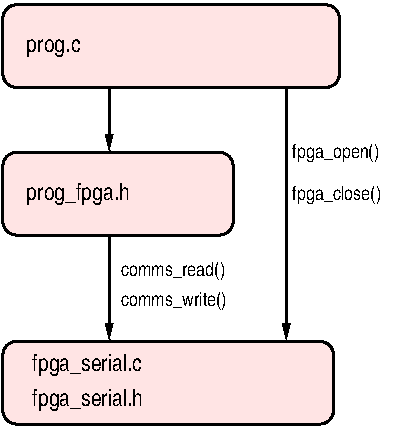
\includegraphics{c_serial}
        
        For details see (\autorefph{ch:tools_c_serial}).
        
        For the .info file listed previously the created include file
        {\bf prog\_fpga.h} contains -

        \begin{lstlisting}[gobble=4, language=C]
            // interface "P" in space "reg" 
            typedef int64_t fpga_P_t;
            const unsigned fpga_P_addr = 2;
            static fpga_P_t
            fpga_P_read() {
                fpga_P_t v;
                comms_read(0, fpga_P_addr, 0, 6, 1, 2, (char *)&v);
                if ((v & 0x800000000000) != 0)
                    v |= 0xffff000000000000;
                return(v);
            }

            // interface "B" in space "reg" 
            typedef int32_t fpga_B_t;
            const unsigned fpga_B_addr = 3;
            static void
            fpga_B_write(fpga_B_t val) {
                comms_write(0, fpga_B_addr, 0, 3, (char *)&val);
            }

            // interface "A" in space "reg" 
            typedef int32_t fpga_A_t;
            const unsigned fpga_A_addr = 2;
            static void
            fpga_A_write(fpga_A_t val) {
                comms_write(0, fpga_A_addr, 0, 4, (char *)&val);
            }

            // event "INT"
            void
            fpga_INT_wait() {
                sem_wait(sem[0]);
            }

            const unsigned fpga_interrupts = 1;
        \end{lstlisting}
        Note that for each interface function the string "fpga\_" is prepended
        to the function identifier.

        At the moment reads and writes of single variables will defines types
        {\bf int8\_t} or {\bf uint8\_t} up to {\bf int\_64\_t} or {\bf uint64\_t}
        for data widths 8, 16, 32 or 64. A struct up to 64 bits in size will be
        mapped to a bit field.
    
        The following C program includes the above file -        

        \begin{lstlisting}[gobble=4, language=C]
            #include <stdio.h>
            #include "cpu_serial.h"

            void*       INT_handler ();

            #include    "prog_fpga.h"

            int
            main (
                int     argc,
                char**  argv
            ) {    
                pthread_t   INT_thread;
                int         pri_min = 1;

                // Establish the CPU interface.
                fpga_open("/dev/tty.usbmodem14201");

                // Start a thread for the interrupt
                INT_thread  = thread_start(INT_handler,  "INT_handler",  pri_min);

                fpga_A_write(123);
                fpga_B_write(1);
                printf("read %lld (should be 123)\n", fpga_P_read());
                fpga_A_write(1);   // will generate an interrupt
                sleep(1);          // wait for the interrupt

                // Close the interrupt thread.
                pthread_cancel(INT_thread);


                // Close the CPU interface.
                fpga_close();

                exit(0);
            }

            void*
            INT_handler () {
                for(;;) {
                    fpga_INT_wait();
                    printf("interrupt INT\n");
                }
            }

        \end{lstlisting}

        The CPU code uses library {\bf cpu\_serial.c} (see appendix
        \ref{ch:cpu_serial}) and hence the application program must be
        linked to cpu\_serial.o.

        Procedure findserialdev() is called to find the file path for the serial
        device to which the FPGA board is connected. In this case the code is
        for Apple OSX and device names will be different in Linux or Unix.

        fpga\_open() opens the serial device, starts
        a thread to handle the communications and establlishes any semaphores
        required for interrupts. Writes to the FPGA do not supply any
        acknowledgement. Data returned from the FPGA included requested reads
        and asynchronous 'interrupts'. Details of the interface are described in
        \autorefph{chap:lmxilcpulib}.

        fpga\_close() terminates the thread, removes any semaphores and
        closes the serial port.

        Bus interfaces are used by calling the appropriate subroutines defined
        in prog\_fpga.h, in this case {\bf fpga\_A\_write()},  {\bf fpga\_B\_write()}
        and {\bf fpga\_P\_read()}, the bus addresses having been subsumed into
        the subroutine definitions.
    



    \section{Python interface}

        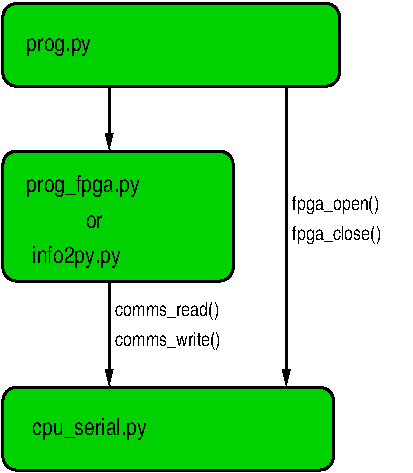
\includegraphics{py_serial}
        
        For details see (\autorefph{ch:tools_python_serial}).
        
        The 3PL module uart\_cpu.3pl will always produce a .info file. A
        compressed version loaded into block RAM in the FPGA configuration will
        also be included by default but can be omitted by creating the directive
        "excludeinfo".
    
        For a Python interface to the FPGA the module {\bf cpu\_serial.py} (in
        directory fpga\_platforms/serial/uart\_cpu must be imported.)
        
        Optionally {\bf info2py.py} (in directory fpga\_platforms/info2py) can
        be imported to convert the .info file to an internal compiled Python3
        module.        If {\bf info2py.py} is imported it either reads the .info
        file (call info\_from\_file(file) or downloads the compressed info data
        in the FPGA (call info\_from\_fpga()) and generates an internal module
        containing functions to access the FPGA register or memory interfaces.

        As an alternative the Python3 script {\bf info2py} can be executed
        to create a Python3 module {\bf prog\_fpga.py} which is then imported
        into the application program. A version of this file
        for the present example is listed below -


        \begin{lstlisting}[gobble=4, language=Python]
            import os
            import math
            import string
            import textwrap
            import argparse
            import json
            import sys
            import time
            sys.path.append(os.environ['HOME'] + '/install/3pl')
            import cpu_serial as fpga_rw

            def B_write(wdata):
                val = wdata 
                if val < 0:
                    wba = val.to_bytes(3, byteorder='little', signed=True)
                else:
                    wba = val.to_bytes(3, byteorder='little')
                fpga_rw.comms_write(0, 3, 0, wba)

            def P_read():
                rba = fpga_rw.comms_read(0, 2, 0, 6)
                val = int.from_bytes(rba, byteorder='little', signed=False)
                fval = val & 0xffffffffffff
                if (fval & 0x800000000000) != 0:
                     fval = -((fval ^ 0xffffffffffff) + 1)
                return(fval)

            def A_write(wdata):
                val = wdata 
                if val < 0:
                    wba = val.to_bytes(4, byteorder='little', signed=True)
                else:
                    wba = val.to_bytes(4, byteorder='little')
                fpga_rw.comms_write(0, 2, 0, wba)

            # event "INT"
            def INT_wait():
                fpga_rw.semaphores[0].acquire()

            def INT_count():
                return(fpga_rw.event_count(0))
        \end{lstlisting}



        cpu\_serial.py provides the code to open the serial interface to the FPGA,
        read and write to the FPGA and generate interrupts if required.

        
        The identifiers of the interface functions are listed in the report file,
        along with the data type. Each function is contained in the CPU\_API class
        {\bf fpga}.
        
        Python source code equivalent to the previous C interface might be -
        \begin{lstlisting}[gobble=4, language=Python]
            import sys
            sys.path.append("/Users/....../install/3pl")
            import info2py
            from cpu_serial import *
            import time
            import signal
            import threading

            fpga_open("/dev/tty.usbmodem14101")

            fpga = info2py.info_from_fpga()         # load info from FPGA

            def INT_handler():
                while True:
                    fpga.INT_wait()
                    print("event INT")

            ev_INT = threading.Thread(target=INT_handler, args=(), daemon=True)
            ev_INT.start()

            a = 123
            b = 1

            fpga.A_write(a)
            fpga.B_write(b)
            print(str(fpga.P_read()) + "\t(should be 123)")
            a = 1
            fpga.A_write(a);    # will generate an interrupt

            time.sleep(1.0)     # wait for the interrupt

            fpga_close()

            os.kill(os.getpid(), signal.SIGTERM)    # use this to kill all threads!
        \end{lstlisting}
        
        In the code above the application program loads the interface information
        from the version embedded in the FPGA in block RAM.
        With the following modification the interface information will be
        loaded from the prog.info file instead.

        
        \begin{lstlisting}[gobble=4, language=Python]
            import sys
            .
            .
            .

            fpga_open("/dev/tty.usbmodem14101")
            
            fpga = info2py.info_from_file("prog")   # load info from prog.info file
            .
            .
            .
        \end{lstlisting}
        
        
        
        Alternatively the following imports a version of the interface function
        definitions created by Python3 script {\bf info2py}.
        
        \begin{lstlisting}[gobble=4, language=Python]
            import sys
            .
            .
            .
            import prog_fpga as fpga    # import interface info from Python3 file

            fpga_open("/dev/tty.usbmodem14101")
            .
            .
            .
            .
        \end{lstlisting}
        
        
        The Python serial interface to the FPGA can read or write variables of
        any type to any degree of nesting, but there is a maximum variable size
        of 1016 bits (the 7-bit byte count in the communication protocol limits
        the data length to 127 bytes). The following type conversions between
        3PL and Python will occur -
         
        \begin{tabular}{| l | l | l |}
        \hline
        FPGA    & Python                \\
        \hline
        log     & logical               \\
        bits    & integer               \\
        uint    & integer               \\
        int     & integer               \\
        ufixed  & IEEE754 64bit float   \\
        fixed   & IEEE754 64bit float   \\
        float   & IEEE754 64bit float   \\
        struct  & dictionary            \\
        array   & list                  \\
        \hline
        \end{tabular}
        
        There are no run-time tests for data integrity, for example overflows.
        
        3PL arbitrary ufixed and fixed integer and fraction sizes are converted
        in or out of IEEE 64 bit floatin point in Python. Similarly 3PL arbitrary
        floating point biased exponent and mantissa sizes are again converted
        in or out of IEEE 64 bit floatin point.
        
        A struct in 3PL is converted in or out of a dictionary in Python, the
        field name being the key.
        
        3PL multi-dimensional arrays are nested lists in Python.

            
\pagebreak

\chapter{Zynq Communication Between the CPU and the FPGA}\label{ch:zynqcpu}

    The following assumes the use of a Linux kernel on the Zynq platform and a
    Linux, Unix or OSX operating system on a host computer for CPU code
    cross-compilation and execution of some of the support programs.
    
    This interface is very similar to the serial CPU interface described in the
    previous chapter (\autorefph{ch:serialcpu}). Much of the code is common to
    both.

    The board file xilinx/zynq\_axi.3pl includes source xilinx/cpu.3pl.
    Procedure create\_bus\_interfaces() in xilinx/zynq\_axi.3pl executes at the
    end of the main code to create the bus interface logic.

    GP bus 0 is used for reading 3PL expressions (i.e. value mode variables) or
    writing 3PL static or queue mode variables. GP bus 1 is used to read or
    write 3PL memory variables. Burst transfers of up to 8 32-bit words are
    supported. The four HP buses are used to implement 64-bit wide DMA transfers
    between the FPGA and CPU. Thus far the default 100MHz clock has been used
    for all buses. The CPU to FPGA interfaces are described in
    \autorefph{chap:lmzynqaxilib}.
    
    For this interface to operate the Zynq Linux device tree must provide
    entries for axi\_mgp0, axi\_mgp1 and axi\_hpbuf and must also provide
    interrupt events 0 to 15. An example is shown in
    \autorefph{ch:zynq_device_tree}.
    
    The following source code, prog.3pl, is an example of a simple 3PL program
    using CPU interfaces -
    
    \begin{lstlisting}[gobble=4, language=threepl]
        module "boards/avnet/microzed_7010.3pl"
        
        class(cpu, cpu_api());  // CPU API class

        static(a, "int:25");
        static(b, "int:18");

        cpu.write(a <- "A");    // write to {\bf a} from CPU
        cpu.write(b <- "B");    // write to {\bf a} from CPU

        static(p, "int:48");

        p <- a * b;

        cpu.read(p, "P");       // read from {\bf p} to CPU

        cpu.receive_event("INT", p == 1);   // interrupt when p == 1
    \end{lstlisting}
    
    Static variables {\bf a} and {\bf b} can be written to by the CPU. The
    product is assigned to p (in every clock cycle), which can be read by the
    CPU. The strings "A", "B" and "P" are names with which to refer to the
    interfaces within CPU code.
    
    Note that the interrupt {\bf INT} occurs when the expression
    {\bf p == 1} goes from false to true.
    
    When the program is compiled and executed by 3pl
    \autorefph{chap:run3pl}) the following files will be produced -
    \blist
    \item   {\bf prog.edif} - netlist file
    \item   {\bf prog.xdc} - Vivado constraints file
    \item   {\bf prog.bit} - configuration bit file
    \item   {\bf prog.info} - CPU/FPGA interface information (JSON) file
    \item   {\bf prog.rpt} - report file
    \item   {\bf prog.net} - optional list of net labels
    \blend
    The bit file is produced by a default post-processing module and can be
    supressed by specifying the -s option (skip) to 3PL. In that case the
    place-and-route can be performed by shell script edif2bit
    (sources/fpga\_platforms/edif2bit/edif2bit) or by the simple bash script
    run\_vivado (sources/fpga\_platforms/run\_vivado).
    
    The configuration file may be compressed using gzip
    
    The configuration file can be loaded into the FPGA manually by
    \verb'cat >/dev/xdevcfg'. Alternatively The configuration file or compressed
    configuration file can be converted into a byte array in CPU application
    code - see below.
    
    The CPU/FPGA interface information file prog.info is in JSON format and
    describes the CPU/FPGA interface.
     
    \begin{verbatim}
        {
            "version": {
                "major": 1,
                "minor": 0
            },
            "directives": {
                "ALU": "false",
                "FIFO": "false",
                "OS": "mac os x",
                "QUEUEREG": "false",
                "arch": "x86_64",
                "compileOnly": "false",
                "compilerMakeDate": "2022-04-04 14:45:06 +1000",
                "continuous": "false",
                "currentDirectory": "/Users/dun202/snark/src/test/zynq_int_test",
                "date": "2022-07-05 10:26:31 +1000",
                "designName": "prog",
                "family": "XC7",
                "filePath": "false",
                "forceExec": "true",
                "gatesNotLuts": "false",
                "intTruncWarning": "false",
                "intermediateOnly": "false",
                "listNets": "true",
                "listTDEs": "true",
                "listTDEsSel": "0",
                "locations": "false",
                "netFile": "/Users/dun202/snark/src/test/zynq_int_test/prog.net",
                "netlistDisplay": "false",
                "netlistFile": "/Users/dun202/snark/src/test/zynq_int_test/prog.edn",
                "optimiseConnect": "true",
                "outputDirectory": "/Users/dun202/snark/src/test/zynq_int_test/",
                "parentDirectory": "/Users/dun202/snark/src/test/zynq_int_test/",
                "part": "xc7z010clg400-1",
                "postProcessCompress": "true",
                "postProcessTool": "vivado",
                "reportFile": "/Users/dun202/snark/src/test/zynq_int_test/prog.rpt",
                "rptToFile": "true",
                "sigList": "false",
                "skipPostProc": "true",
                "sourceFile": "prog.3pl",
                "srlAddrWidth": "5",
                "unassOut": "fatal",
                "version": "11.7.0M (devel svn 10011:10036M, dun202)"
            },
            "spaces": {
                "reg": {
                    "bus": "axi_mgp0",
                    "read_addr_bits": 2,
                    "write_addr_bits": 2,
                    "interfaces": {
                        "infoword": {
                            "interface": "read_value",
                            "write": false,
                            "data_addr": 1,
                            "data_bits": 32,
                            "data_type": {
                                    "type": "uint",
                                    "bits": 32
                            }
                        },
                        "inforeset": {
                            "interface": "write_static",
                            "write": true,
                            "data_addr": 1,
                            "data_bits": 0
                        },
                        "A": {
                            "interface": "write_static",
                            "write": true,
                            "data_addr": 2,
                            "data_bits": 25,
                            "data_type": {
                                    "type": "int",
                                    "bits": 25
                            }
                        },
                        "B": {
                            "interface": "write_static",
                            "write": true,
                            "data_addr": 3,
                            "data_bits": 18,
                            "data_type": {
                                    "type": "int",
                                    "bits": 18
                            }
                        },
                        "P": {
                            "interface": "read_value",
                            "write": false,
                            "data_addr": 2,
                            "data_bits": 48,
                            "data_type": {
                                    "type": "int",
                                    "bits": 48
                            }
                        }
                    }
                }
            },
            "events": {
                "INT": {
                    "intr": 0
                }
            }
        }

    \end{verbatim}
    This file contains a description of the CPU bus interfaces including data
    width, data type and allocated bus addresses.

    A list of the interface functions is also written to the report file.

    The design.info data may also be stored in block RAM (rmemory) for access by
    CPU code. This is enabled by default but may be avoided via a directive,
    i.e. {\bf directive("excludeinfo", true);}, which can be executed at any
    time during 3PL immediate execution. The compression is done by calling
    inbuilt function {\bf deflate()} \autorefph{sec:ifdeflate}. The readback is
    initialised by writing to address 1 and 32-bit packed .info data is then
    read by successive 32-bit reads from address 1. The first read returns a 32
    bit CRC-32 checksum for the remainder of the block,\. The second read
    returns the uncompressed data size in bytes and the third read returns the
    compressed data size in bytes. Reads beyond the data length will return
    zeros.

    The data block size depends on the size of the compressed .info data and
    varies from a minimum of 1024 32 bit words (1 RAM block) to 32,768 words (32
    RAM blocks).

    For C applications the .info file must be converted to a C include file by
    utility {\bf info2c}. That include file defines functions and procedures to
    read and write to specified FPGA variables.

    For Python3 applications the .info file cab be converted by {\bf info2py} to
    a Python3 file that can be imported into the python application.
    Alternatively {\bf info2py} can itself be imported into the python application
    and it can then read th .info file or read out the embedded version in
    the FPGA.
    
    \section{C interface}
    
        The configuration bit file can be manually loaded into the FPGA
        by {\bf \verb'cat prog.bit >/dev/xdevcfg'}.
    
        The configuration data can instead be incorporated into the CPU
        application program by using the utility {\bf bin2c}
        (sources/fpga\_platforms/bin2c). This will create an include file {\bf
        prog\_cinclude.h}. Although the uncompressed configuration file prog.bit
        can be used it is clearly preferable to use the compressed configuration
        file prog.bit.gz. The configuration data can then be loaded into the FPGA
        by the application program by calling {\bf fpga\_configdata\_load()} as
        illustrated later.
        
        Alternatively the application program can load the FPGA configuration
        from the configuration file prog.bit or prog.bit.gz by {\bf
        fpga\_configfile\_load("prog.bit")} or {\bf
        fpga\_configfile\_load("prog.bit.gz")}.
    
        When the {\bf prog.info} file is processed by the python script {\bf
        info2c} (sources/fpga\_platforms/zynq/info2c/info2c) by {\bf
        \verb'info2c prog'} a C include file, {\bf prog\_fpga.h}, results.

        \begin{lstlisting}[gobble=4, language=C]
            // event "INT"
            static __inline__ void
            fpga_INT_enable() {
                fpga_event_control(0, 1);
            }
            static __inline__ void
            fpga_INT_disable() {
                fpga_event_control(0, 0);
            }
            static __inline__ void
            fpga_INT_wait() {
                fpga_event_wait(0);
            }
            static __inline__ int
            fpga_INT_count() {
                return(uio_event_count(0));
            }

            // interface "A" in space "reg" (bus "axi_mgp0")
            typedef int32_t fpga_A_t;
            const unsigned fpga_A_addr = 4;
            static __inline__ void
            fpga_A_write(fpga_A_t val) {
                FPGA_REG_WRITE(fpga_A_addr, val, 1);
            }

            // interface "P" in space "reg" (bus "axi_mgp0")
            typedef int64_t fpga_P_t;
            const unsigned fpga_P_addr = 2;
            static __inline__ fpga_P_t
            fpga_P_read() {
                FPGA_REG_READ(fpga_P_addr, fpga_P_t, 2);
            }

            // interface "B" in space "reg" (bus "axi_mgp0")
            typedef int32_t fpga_B_t;
            const unsigned fpga_B_addr = 6;
            static __inline__ void
            fpga_B_write(fpga_B_t val) {
                FPGA_REG_WRITE(fpga_B_addr, val, 1);
            }

            // space and event bitfield for fpga_map() 2nd argument
            #define fpga_map_needed \
                fpga_map_none \
                | fpga_space_reg \
                | fpga_INT_event
        \end{lstlisting}

        At the moment reads and writes of single variables will defines types
        {\bf int8\_t} or {\bf uint8\_t} up to {\bf int\_64\_t} or {\bf uint64\_t}
        for data widths 8, 16, 32 or 64. A struct up to 64 bits in size will be
        mapped to a bit field. To transfer bursts larger than 2 (64 bits) subroutines
        {\bf FPGA\_REG\_READ()} and {\bf FPGA\_REG\_WRITE()} can be called directly
        for bursts up to 8 32-bit words. In that case the bus address must be determined
        from the .info file and passed explicitly.
        
        This file, {\bf prog\_fpga.h}, defines functions which specifically read or
        write interface objects in the FPGA. These funtions in turn call
        functions in the communications layer defined by {\bf cpu\_serial.c},
        {\bf cpu\_serial.h}. Some function such as {\bf open\_cpu\_serial()} and
        {\bf close\_cpu\_serial()} are call directly skipping {\bf prog\_fpga.h}.
        

        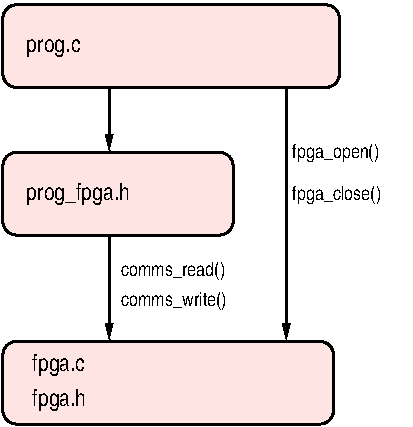
\includegraphics{c_zynq}
        
        For details see (\autorefph{ch:tools_c_zynq}).

        The following C program includes the above file. Note that in the case of
        a Python3 program the interface information can be read from the FPGA and
        compiled as a module If the interface information has been incorporated
        into block RAM in the FPGA. This cannot be done with a C interface and
        thus directive "excludeinfo" should be set true to avoid wasting these
        logic and memory resources;
        
        \begin{lstlisting}[gobble=4, language=C]
            #include <stdio.h>
            #include <stdlib.h>
            #include <stdint.h>
            #include <pthread.h>
            #include "/root/install/3pl/fpga.h"

            int64_t     p;

            void*       INT_handler ();
            pthread_t   thread_start(
                            void *  (*func)(void*),
                            void *  arg,
                            char *  name,
                            int     priority
                        );

            #include    "prog_cinclude.h"

            #include    "prog_fpga.h"

            int
            main (
                int     argc,
                char**  argv
            ) {    
                pthread_t   INT_thread;
                int         pri_min = 1;

                // Open the CPU interface.
                fpga_open();

                // Load the configuration.
                //fpga_configdata_load(prog_fpga_config_data, prog_fpga_config_size);
                fpga_configfile_load("prog.bit");

                // Start a thread for the interrupt
                INT_thread  = thread_start(INT_handler,  NULL, "INT_handler",  pri_min);

                fpga_A_write(123);
                fpga_B_write(1);
                p = fpga_P_read();
                printf("read %lld (should be 123)\n", p);
                fpga_A_write(1);   // will generate an interrupt
                sleep(2);          // wait for the interrupt
                fpga_B_write(2);
                fpga_B_write(1);   // will generate another interrupt

                // Terminate the interrupt thread.
                pthread_cancel(INT_thread);


                // Close the CPU interface.
                fpga_close();

                exit(0);
            }

            void*
            INT_handler () {
                for(;;) {
                    fpga_INT_enable();
                    fpga_INT_wait();
                    printf("interrupt INT, p = %lld\n", p);
                    printf("number of events %d\n", fpga_INT_count());
                }
            }


            // Start a thread.
            pthread_t
            thread_start(
                void *  (*func)(void*),
                void *  arg,
                char *  name,
                int     priority
            ) {
                int                 status;
                struct sched_param  sp;
                pthread_t           tid;

                if ((status = pthread_create(&tid, NULL, func, arg)) != 0) {
	            printf("thread_start(): pthread_create() failed thread '%s' (err = %s)\n",
	                name, strerror(status));
                    exit(1);
                }

                sp.sched_priority = priority;

                status = pthread_setschedparam(tid, SCHED_RR, &sp);
                if (status != 0) {
    	            printf("thread_start(): pthread_setschedparam() failed for thread '%s' (err = %s)\n",
	                name, strerror(status));
                    exit(1);
                }
                return(tid);
            }
        \end{lstlisting}

        Include file "fpga.h" defines the basic FPGA communication interface
        functions.
        
        Include file "prog\_fpga.h" is created by python script 'info2c' and contains
        function definitions for each FPGA read, write or interrupt (event).
        These in turn use the functions in fpga.h above.

        {\bf fpga\_open()} sets up the ARM memory mapping for the AXI buses and devices
        associated with interrupts (events).

        {\bf fpga\_configdata\_load()} loads the FPGA configuration.  In this example
        the compressed FPGA configuration is compiled into the CPU program and is
        included from the file {\bf prog\_cinclude.h}. That file has been created by
        running program {\bf bin2c} which takes the configuration file prog.bit
        compresses it and then converts it to an array of hexadecimal constants. The
        FPGA configuration can alternatively be loaded from a file by the CPU if
        desired by calling {\bf fpga\_configfile\_load()} instead.

        Bus interfaces are used by calling the appropriate subroutines defined in prog\_fpga.h,
        in this case {\bf fpga\_A\_write()}, {\bf fpga\_B\_write()} and {\bf
        fpga\_P\_read()}, the bus addresses having been subsumed into the subroutine
        definitions. These functions are defined in 'prog\_fpga.h'.
        
        The C program must be linked with object file 'fpga.o' which can be
        compiled from source file 'fpga.c' located in the 3PL source directory
        'sources/fpga\_platforms/zynq/fpga'.



    \section{Python interface}

    
        As described previously the configuration file can be loaded into the
        FPGA manually by {\bf \verb'cat prog.bit >/dev/xdevcfg'}. Alternatively
        the configuration file prog.bit or compressed configuration file
        prog.bit.gz  can be converted into a byte array in source code.
    
        The configuration data can be incorporated into the CPU application
        program by using the utility {\bf bin2py} (sources/fpga\_platforms/bin2py).This
        will create a source file {\bf prog\_config.py} which can be
        imported into the application program.
        The configuration data can then be loaded into the FPGA by the
        application program by calling {\bf fpga\_configdata\_load()} -
        \begin{lstlisting}[gobble=4, language=Python]
            fpga_configdata_load(config.data, len(config.data))
        \end{lstlisting}
        
        The configuration can also be loaded from the uncompressed or compressed
        bit file during execution of the application program by calling {\bf
        fpga\_configfile\_load()}-
        \begin{lstlisting}[gobble=4, language=Python]
            fpga_configfile_load("prog.bit.gz"))
        \end{lstlisting}
        or
        \begin{lstlisting}[gobble=4, language=Python]
            fpga_configfile_load("prog.bit"))
        \end{lstlisting}
        

        
        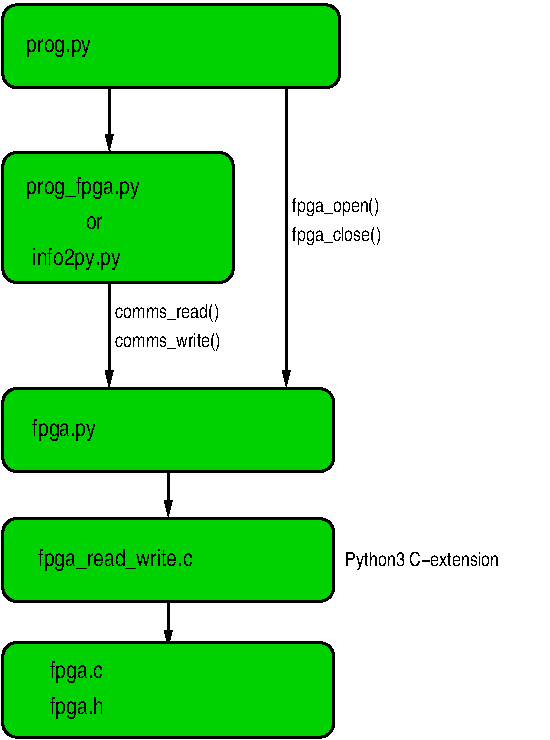
\includegraphics{py_zynq}
        
        For details see (\autorefph{ch:tools_python_zynq}).


    
        For a Python interface to the FPGA the modules {\bf info2py.py} (in
        directory fpga\_platforms/info2py) and functions in {\bf fpga.py} (in
        directory fpga\_platforms/zynq/fpga) must be imported.

        Functions in {\bf fpga.py} provide the code to open the interface to the
        FPGA, read and write to the FPGA and generate interrupts if required.

        info2py.py either reads the .info file (call info\_from\_file(file) or
        downloads the compressed info data in the FPGA (call info\_from\_fpga())
        and generates an internal module containing functions to access the FPGA
        register or memory interfaces.
        
        The 3PL module zynq\_axi.3pl will always produce a .info file. The
        compressed version loaded into block RAM in the FPGA configuration will
        be included by default but can be omitted by creating the directive
        "excludeinfo".
        
        The identifiers of the interface functions are listed in the report file,
        along with the data type. Each function is contained in the CPU\_API
        class {\bf fpga}.
    
        The previous 3PL source code can be used again as an example.

        The following Python source code would provide a CPU interface to the
        FPGA. The configuration file prog.bit is loaded into the FPGA by
        the application code by .
        
        The CPU/FPGA interface functions are defined
        in imported module {\bf prog\_fpga.py} which has been created by
        {\bf info2py prog}.
        
        {\bf fpga\_configfile\_load("prog.bit")}. This
        line could be omitted if the configuration was manually preloaded
        by executing {\bf cat prog.bit \verb'>'/dev/xdevcfg}.

        \begin{lstlisting}[gobble=4, language=Python]
            import sys
            import os
            sys.path.append(os.environ['HOME'] + "/install/3pl")
            from fpga import *
            import prog_fpga as fpga
            import time
            import signal
            import threading

            fpga_configfile_load("prog.bit")

            fpga_open()

            def INT_handler():
                while True:
                    fpga.INT_wait()
                    print("event INT")
                    print("number of events " + str(fpga.INT_count()))


            ev_INT = threading.Thread(target=INT_handler, args=(), daemon=True)
            ev_INT.start()

            a = 123
            b = 1

            fpga.A_write(a)
            fpga.B_write(b)
            print(str(fpga.P_read()) + "\t(should be 123)")
            a = 1
            fpga.A_write(a);    # will generate an interrupt
            a = 2
            fpga.A_write(a);
            a = 1
            fpga.A_write(a);    # will generate an interrupt

            time.sleep(1.0)     # wait for the interrupts

            fpga_close()

            os.kill(os.getpid(), signal.SIGTERM)    # use this to kill all threads!
        \end{lstlisting}

        As an alternative the configuration could be stored within the application
        code as an initialised byte array. Executing {\bf bin2py prog} will
        take prog.bit.gz and produce a Python3 module {\bf prog\_config.py}
        which can be imported to define the CPU/FPGA interface.


        \begin{lstlisting}[gobble=4, language=Python]
            import sys
            import os
            sys.path.append(os.environ['HOME'] + "/install/3pl")
            from fpga import *
            import prog_fpga as fpga
            import time
            import signal
            import threading
            import prog_config as config

            fpga_configdata_load(config.data, len(config.data))

            fpga_open()

            .
            .
            .

        \end{lstlisting}

        Instead of the CPU/FPGA interface definitions being imported
        from file {\bf prog\_fpga.py} as above they can be read from 
        {\bf prog.info} during execution using module {\bf info2py.py}.


        \begin{lstlisting}[gobble=4, language=Python]
            .
            .
            import info2py
            .
            .
            fpga_open()

            fpga = info2py.info_from_file("prog")   # load info from prog.info file
            .
            .
        \end{lstlisting}

        Another possibility is to import the CPU/FPGA interface definitions from
        the interface description embedded in the FPGA, assuming this has not
        been omitted by the directive "excludeinfo" true -


        \begin{lstlisting}[gobble=4, language=Python]
            .
            .
            import info2py
            .
            .
            fpga_open()

            fpga = info2py.info_from_fpga()         # load info from FPGA
            .
            .

        \end{lstlisting}
        
        The additional Python3 package path "/Users/..../install" depends on
        the layout of the file system, but the path component must contain
        "fpga.py" and "info2py".

        The Python3 library module {\bf fpga.py} must have been added by
        executing shell script {\bf mk\_setup} in {\bf ~/install/3pl/} on the
        Zynq CPU. This script runs setup.py which creates and adds the library
        module fpga\_py\_extension.c. Both {\bf setup.py} and {\bf mk\_setup} are installed in {\bf
        ~/install/3pl/setup.py}and the sources are in {\bf sources/tools/zynq}
        
        The Python CPU interface to the FPGA can read or write variables of any
        type to any degree of nesting, but there is a maximum variable size of 256
        bits (ldm/stm using 8 registers for a burst transfer). The following type
        conversions between 3PL and Python will occur -
         
        \begin{tabular}{| l | l | l |}
        \hline
        FPGA    & Python                \\
        \hline
        log     & logical               \\
        bits    & integer               \\
        uint    & integer               \\
        int     & integer               \\
        ufixed  & IEEE754 64bit float   \\
        fixed   & IEEE754 64bit float   \\
        float   & IEEE754 64bit float   \\
        struct  & dictionary            \\
        array   & list                  \\
        \hline
        \end{tabular}
        
        There are no run-time tests for data integrity, for example overflows.
        
        3PL arbitrary ufixed and fixed integer and fraction sizes are converted
        in or out of IEEE 64 bit floatin point in Python. Similarly 3PL arbitrary
        floating point biased exponent and mantissa sizes are again converted
        in or out of IEEE 64 bit floating point.
        
        A struct in 3PL is converted in or out of a dictionary in Python, the
        field name being the key.
        
        3PL multi-dimensional arrays are nested lists in Python.

    \section{An aside}

        As a matter of interest the following C function illustrates retrieval of the information string
        from the FPGA. The string length is returned as the function value and
        a pointer to the information string is assigned to the pointer argument.
        It is not necessary to use this function normally as the .info file can be
        converted to a C include file by using Python script 'info2c' as explained
        previously.

        \begin{lstlisting}[gobble=4, language=C]
           int fetch_info (unsigned char ** info) {
               int             i;
               int             n;
               int             e;
               unsigned long * buf;
               unsigned char * ubuf;
               unsigned long * bufp;
               unsigned long   ulen;

               fpga_reg_write(1, 0);
               n = fpga_reg_read(1);    // number of bytes of compressed data
               ulen = n * 10;           // enough room for uncompressed data (a guess)

               buf = malloc(n+3);       // enough room for compressed data, 32-bit packed
               ubuf = malloc(ulen);
               bufp = buf;
               for (i=0 ; i<n ; i+=4)
                   *bufp++ = fpga_reg_read(1);

               e = uncompress(ubuf, &ulen, ((Byte *)buf), n);
               if (e != Z_OK) {
                   printf("info uncompress error %d\n", e);
                   return(-1);
               }

               free(buf);
               *info = realloc(ubuf, ulen); // eliminate unused trailing buffer space
               return(ulen);
           }
        \end{lstlisting}
        
        But alas in C this interface information cannot be used, as it can in
        Python3.

        In the case of Python3, the following code would retrieve the JSON info
        from the FPGA data as a string -


        \begin{lstlisting}[gobble=4, language=Python]
            #----------------------------------------------------------------------
            # Read the compressed JSON structure from the FPGA
            # and expand it. Return a code module containing the interface
            # functions.
            #
            def info_from_fpga ():
                # reset the json interface
                fpga_rw.comms_write(0, 2, 0, None)

                # get the checksum
                rba = fpga_rw.comms_read(0, 1, 0, 4)
                checksum = int.from_bytes(rba, byteorder=bo, signed=False)

                # get the uncompressed byte count
                rba = fpga_rw.comms_read(0, 1, 0, 4)
                ucl = int.from_bytes(rba, byteorder=bo, signed=False)

                # get the compressed byte count
                rba = fpga_rw.comms_read(0, 1, 0, 4)
                cl = int.from_bytes(rba, byteorder=bo, signed=False)

                # read the compressed json info string
                words = cl // 4 + 1
                rba = bytearray()
                for i in range(words):
                    rba += fpga_rw.comms_read(0, 1, 0, 4)

                # decompress the json string
                infostring = zlib.decompress(rba[2:-4], -15)

                return(str(infostring, 'utf-8'))
        \end{lstlisting}




\pagebreak

\chapter{Using EDIF Cores}

    By 'core' is meant an EDIF netlist file which implements a logic
    function but is not itself a complete logic design.
    
    Note: in the case of the Zynq platform the EDIF file must be a core,
    the bi-directional ports being connected to resources external to the
    FPGA. The CPU interface is incorporated as a large cell called "PS7". 
    
    A Xilinx core EDIF netlist file contains an interface description
    which lists the input and output (and 3-state) connections to the core
    logic. As an example the following core was generated using
    Xilinx coregen -

    \begin{figure}[htbp]
    \centering
    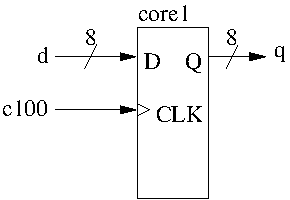
\includegraphics{core1}
    \end{figure}

    This is a simple 8-bit register. The core is called "core2" and
    has the following inputs and outputs -

    \begin{tabular}{l l l}
    port & width & direction \\
    \hline
    D   & 8 & input \\
    CLK & 1 & input \\
    Q   & 8 & output \\
    \end{tabular}

    Note that the use of upper case identifiers for ports seems to be a
    convention with Xilinx but is not required by 3PL.
    
    NGC files are generated from {\bf coregen} via {\bf xst} and are
    linked in by {\bf ngdbuild}.
    
    Note that the core may have an associated constraints file and this can
    be added to a constraints file generated by 3PL by means of library
    procedures {\bf append\_ncf\_file()} \autorefph{sec:lpappncf}.

    \section{linking in EDIF or NGC cores}

        The following 3PL hymod program illustrates how this core can be
        used -
        \begin{lstlisting}[gobble=8, language=threepl]
           module "csiro/hymod/io1.3pl"

           useclock(c100);

           var(ipins, "[]str", {......});
           var(opins, "[]str", {......});
           static(s, "uint:8"); 
           output(,, s, {loc=opins});
           input(d, "uint:8", {loc=ipins});
           value(q, "uint:8");

           import(Q=q <- "core1", CLK=c100, D=d);
           attributes(q, domain=c100);

           s <- q;
        \end{lstlisting}

        Input ports can be driven by expressions or variables of mode
        input, value, static, priority or clock.

        Variables connected to the output ports of the core can only
        be clock, value or selectvalue (for 3-state) mode. Output
        variables to {\bf import()} will not have a clock domain. It may be
        set explicitly by {\bf domain()} as in the example above, otherwise
        variables with no clock domain will not be checked against
        the current clock when evaluated. Note that this does not invalidate
        timing constraints which are set up according to which clocks state
        devices are actually clocked by in the final netlist.
        \index{constraint!timing}
        \index{timing constraint}

        Variables can be arrays or structs.

        The number of bits in each argument must exactly match the
        associated core port width.

        Where a clock is sourced in the core and is connected to the
        main program via {\bf import()} the clock variable must
        be created in the main program, e.g.
        \begin{lstlisting}[gobble=8, language=threepl]
           clock(c, frequency=10e6, tnm="C");
           useclock(c);

           value({d, q}, "uint:8");
           static(s, "uint:8");

           import(Q=q, CLK=c <- "core2", D=d);

           s <- q;
        \end{lstlisting}
        All input ports must be connected but connections to unwanted output
        ports may be omitted.

        To place and route the first example above the procedure is no
        different to usual, e.g.
        \begin{verbatim}
        ngdbuild main
        \end{verbatim}
        Ngdbuild will expect to find a file "core1.edn" which it will link
        in to main.edn.
            
    \section{creating EDIF cores}
    
        To create a core EDIF netlist file the inbuilt procedure {\em export()}
        is called. This generates the interface which enables the core to be
        linked to other EDIF netlist files. As an example -
        \begin{lstlisting}[gobble=8, language=threepl]
           source "xilinx/common.3pl"  // to get declaration of part()
           part("........"); // so core references correct Xilinx element library
           
           clock(c);

           useclock(c);

           static(a, "log");
           static(b, "uint:8");
           value(v1, "log");
           value(v2, "uint:8");

           a <- v1;
           b <- v2;

           export(PA=a, PB=b <- CLK=c, PV1=v1, PV2=v2);
        \end{lstlisting}
        \begin{figure}[htbp]
        \centering
        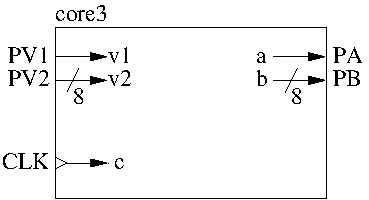
\includegraphics{core3}
        \end{figure}
        In this case {\em PA} and {\em PB} are output ports from this
        core and these are driven by static variables {\em a} and {\em b}.
        The core takes inputs from ports {\em CLK}, {\em PV1} and {\em PV2}.
        The clock variable {\em c} is brought in to the core from outside.
        
        Since the clock {\em c} has an external source we do not have to supply
        a DLL or DCM but we still have to create the clock variable {\em c}
        that is to be connected to the external clock source. The call {\bf
        useclock()} need not precede the {\em export()} call.
        
        The core name must have been supplied using the -e option to the 3PL
        call. This name will also be used for the netlist and constrint outut
        files.


\pagebreak

\chapter{Accessing Specific FPGA Hardware Elements}\label{chap:asfpgahe}
    
    FPGA hardware elements can be created directly from 3PL source code.
    This can be done for the usual common elements that would normally be
    utilised during code generation or for little used or new elements that
    are not directly used by the code generator.
    
    {\bf Note that state elements, such as flip-flops and RAMs, created this way are
    outside the control of the normal execution thread mechanism.}
    
    There are
    three main reasons for using these directly created elements -
    \begin{itemize}
    \item   Special elements such as Virtex4 I/O serial/parallel converters
            cannot be directly incorporated into the semantics of the language.
    \item   We may wish to use low-level components whose inputs are
            not connected to a normal 3PL execution thread, for example a
            flip-flop whose clock enable or reset inputs are connected directly
            to some source.
    \item   We may wish to use absolute or relative placement of components,
            something which is very limited in 3PL proper.
    \item   The compiler may produce combinatorial logic which is sub-optimal
            and which in a critical case needs to be replaced by hand-coded
            logic.
    \end{itemize}
    In such cases we could wrap the created elements in a 3PL module,
    procedure or function to provide a normal 3PL code interface to hide
    these specialised constructs.
    
    As an example library io.3pl creates elements that are common to
    many FPGAs. These include IDDR, ODDR, IDELAY, IODELAY, IDELAYCTRL,
    ISERDES, SYSMON and some DSP functions. These are all created by the
    mechanism described below.
    
    Where an element is required which is not included in a library the
    following inbuilt procedures can be used to create it - \\
    {\bf element()} \autorefph{sec:ipelement}, \\
    {\bf elementend()} \autorefph{sec:ipelementend}, \\
    {\bf elementproperty()} \autorefph{sec:ipelementproperty}, \\
    {\bf elementinput()} \autorefph{sec:ipelmntin}, \\
    {\bf elementclockinput()} \autorefph{sec:ipelmntinclk} \\
    {\bf elementoutput()} \autorefph{sec:ipelmntout} \\
    {\bf elementtsoutput()} \autorefph{sec:ipelmntoutts}.
    
    The inbuilt procedure {\bf elementproperty()} only takes strings as
    value arguments so a number of library procedures are available
    in xilinx/common.3pl to format other types. These are - \\
    {\bf elementLogProperty()} \autorefph{sec:lpelementLogProperty}, \\
    {\bf elementIntProperty()} \autorefph{sec:lpelementIntProperty}, \\
    {\bf elementBinProperty()} \autorefph{sec:lpelementBinProperty}, \\
    {\bf elementHexProperty()} \autorefph{sec:lpelementHexProperty}, \\
    {\bf elementFloatProperty()} \autorefph{sec:lpelementFloatProperty}, \\
    {\bf elementStrProperty()} \autorefph{sec:lpelementStrProperty}
    
    As an example if we wished to directly use a CLB shift register instead of
    using using it implicitly with {\bf del()}, we could create it by -
    \begin{lstlisting}[gobble=4, language=threepl]
       string(id, "srl123");
       element("SRL16E", id);
    \end{lstlisting}
    where
    "SRL16E" is the name of the element in the Xilinx library and "srl123" is an
    optional identifier for the element.
    We would now connect up each of its ports -
    \begin{lstlisting}[gobble=4, language=threepl]
       value({d, ce, q}, "log");
       static(a, "uint:4");
       d := .....;
       a <- .....;

       elementinput(id, "D", d);
       elementinput(id, "A", a, 1);
       elementclockinput(id, "CLK", currentclock());
       elementinput(id, "CE", ce);
       elementoutput(q <- id, "Q");
       elementend(id);
       .... <- q;
       .
       .
    \end{lstlisting}
    We could have omitted the {\bf id} argument in all the calls above in which
    case the currently open element would have been correctly implied.

    
    The call to {\bf element()} creates the element which is retained until the
    next call to {\bf element()} as the current element. Calls to {\bf
    elementinput()}  or {\bf elementoutput()} with no {\bf id} apply to the
    current element. When an id is explicitly used then multiple elements can
    be created using interleaved calls to the above procedures, though there is
    probably little advantage in doing that. The arguments to {\bf
    elementinput()} are -
    \begin{itemize}
    \item   the optional element id (string)
    \item   the port name (string)
    \item   the signal variable
    \item   an array format indicator (integer 0 for single signal, 1 for an array
            where the pins are specified individually, e.g.
            {\bf (port A0 (direction INPUT))} or 2 for an EDIF
            array format such as {\bf (port (array (rename A "a[0:11]") 12) (direction INPUT)))}.
            Unfortunately the required format seems to depend on whether ISE or
            Vivado are used and also on the specific element.
    \end{itemize}
    Input signal variables can be the constants true or false, any value,
    selectvalue, static or priority variable or an expression. The signal cannot be
    from a queue read or an expression containing a queue read but can be from a queue
    variable if the examine operator \verb'?' is used.
    
    This process is subject to the following observations -
    \begin{enumerate}
    \item   The variables or constants are not checked against the port
            type for validity, e.g. if an output port was connected to a
            constant or a static (i.e. the output of the static) this
            would not be detected until code generation time when a fatal
            error resulting from multiple net sources would occur.
    \item   Errors may not be detected until the Xilinx place-and-route
            software is run at which point an obscure error message
            would be generated.
    \item   Elements generated this way cannot be handled by the simulator
            (howevere the simulator is obsolete and not currently available).
    \end{enumerate}

    In the example above it would have been sensible to construct a module or
    procedure so that the code could be reused, for example - 
    \begin{lstlisting}[gobble=4, language=threepl]
       module
       srl16 (value(out) <- value(in), value(ce, "log"), value(addr, "uint:4")) {
           element("SRL16E");
           elementinput(, "D", in);
           elementinput(, "A", addr, 1);
           elementclockinput(, "CLK", currentclock());
           elementinput(, "CE", ce);
           elementoutput(out <- , "Q");
           elementend();
       }
    \end{lstlisting}
    It makes no difference if this is a module or procedure as there is no in-line
    code and no queue reads or writes and the calling syntax and argument passing
    for these are identical.
    
    To implement a similar delay for say an 8-bit integer -
    \begin{lstlisting}[gobble=4, language=threepl]
       module
       srl16_8 (value(out, "int:8") <- value(in, "int:8"), value(ce, "log"), value(addr, "uint:4")) {
           value(o, "[8]bits:1");
           for (int(i) ; i<8 ; i++)
               srl16(o[i] <- getbit(in, i), ce, addr); 
           out := cast(o, "int:8");
       }
    \end{lstlisting}
    To access single bits of the input the library function getbit() (stdlib.3pl)
    has been used. There is no equivalent for assigning bits to the output so a
    local array of single bits has been defined and then this was cast to the
    output type.
    
    The following code is a simplified example of the use of such a delay. To avoid
    complicating the example the inputs are assumed to be synchronous with the
    current clock. 
    \begin{lstlisting}[gobble=4, language=threepl]
       iopins(io_pins, "[20]str", {"AB12", "AC13", .......});
       
       input(din, "int:8", loc=io_pins[0..7], readdomain=null);
       input(dvalid, "log", loc=io_pins[8], readdomain=null);
       static(sum, "int:8");
       value(del, "int:8");
       value(step, "log");

       srl16_8(del <- din, step, 5);

       when (dvalid) par {
           sum <- din + del;
           assert(step <-);
       }

       output(,, sum, loc=io_pins[9..16]);
    \end{lstlisting}
    
    In the above example the clock enable is sourced from an instance of the {\bf
    assert()} \autorefph{sec:ipassert} inbuilt procedure. This procedure asserts the
    output when the execution stream in which it is contained executes.
    
    Alternatively the SRL16E CE could have been driven directly from variable
    {\bf dvalid}.
    
    \begin{lstlisting}[gobble=4, language=threepl]
       .
       .
       srl16_8(del <- din, dvalid, 5);

       when (dvalid)
           sum <- din + del;
       .
       .
    \end{lstlisting}



\pagebreak

\chapter{Constraints, Properties and Attributes}\label{chap:cpa}
    \index{constraint}
    \index{property}
    \index{attribute}
    
    These three terms are used somewhat interchangeably by Xilinx.
    Some constraints/properties/attributes are generated automatically by 3PL.
    These are -
    \begin{enumerate}
    \item   input and output port locations
    \item   CLB memory initialisation
    \item   block memory initialisation
    \end{enumerate}
    These are written to the EDIF file as properties on instances of elements.
    
    All other constraints are generated by 3PL code, in the case of Xilinx in
    library xilinx/common.3pl. The constraints are written to the NCF file in the
    case of ISE or an XDC file for Vivado.
    
    Input and output connections have location constraints generated if a {\bf
    loc} attribute has been set for the input or output mode variable. Attributes
    {\bf ibufdelay}, {\bf ifddelay}, {\bf tnm}, {\bf pullup}, {\bf pulldown},
    {\bf differential}, {\bf diff\_term}, {\bf iostandard}, {\bf ibufg}, {\bf
    slew}, {\bf drive}, if set, also result in constraint file entries.  
    Inbuilt procedures {\bf input()} \autorefph{sec:ipinput}, {\bf
    output()} \autorefph{sec:ipoutput} and {\bf clock()} \autorefph{sec:ipclock} do
    not directly generate these constraints; for convenience and flexibility they
    are handled in 3PL software.

    While attributes can be passed directly to inbuilt procedures {\bf input()},
    {\bf output()} and {\bf clock()}, they may also be associated with the input pins. This
    is done by using the library procedure {\bf iopins()}
    \autorefph{sec:lpiopins} to create variables which contain strings naming the
    FPGA I/O pins (locations). {\bf iopins()} also creates a global map {\bf
    pinAttributes} whose entry keys are I/O pin names, the associated values
    being attribute maps whose keys are attribute identifiers and values the
    attribute values.

    A 3PL user-defined procedure to extract these pin-associated attributes can be
    automatically called whenever an input, output or clock mode variable is
    created. The Xilinx 3PL libraries contain such a procedure, {\bf
    processPinAttributes()} \autorefph{sec:lpprocPinAtt}. This procedure reads the
    pin locations (loc attribute) from the variable and then reads the attribute
    map for each pin, adding these attributes to the attribute map for the
    variable. Note that these pin-related attributes will be overridden by
    attributes passed as arguments to input(), output() or clock(). {\bf
    processPinAttributes()} also ensures that attributes are converted from single
    value to per-pin arrays where appropriate.

    The above procedure must be registered with 3PL so that it can be called by
    the system when an input, output or clock mode variable is created. This is
    done by calling inbuilt procedure {\bf attributeprocedure()}
    \autorefph{sec:ipattributeproc} with a pointer to the procedure as
    argument. Clearly this should be done before any of the above I/O procedures
    are called, preferably be placing a call to {\bf attributeprocedure()} early
    in a leader module.

    While netlist generation attributes are handled by input(), output() of
    clock() following completion of immediate execution, constraint file
    attributes must be handled by 3PL software. This is done by library procedure
    {\bf generateConstraints()} \autorefph{sec:lpgenerateconstraints}. This
    procedure should be called late in a trailer module to ensure that no more
    calls to input(), output() or clock() will be executed. This procedure calls
    inbuilt function {\bf varlist()} \autorefph{sec:ifvarlist} which returns a
    list of target mode variables. The resulting list is traversed and the
    constraint-related attributes of input, output and clock mode variables are
    extracted and constraints are written to the constraints file.   
    
    An example of constraints that might need to be generated explicitly are
    input and output delays where combinatorial logic paths are included - see
    \autorefph{sec:input_output}.
    
    The clock timing group identifier can be explicitly set using a clock
    attribute (tnm), otherwise it will be constructed from the
    clock identifier. Regardless of whether a frequency or period attribute
    has been set a period constraint will be generated. If no frequency
    or period attribute has been set a warning message will be produced to
    the effect that there will be no timing constraints for that clock.
    
    CLB RAM and block RAM initialisation entries are added to the
    EDIF file. If no initialisation is supplied to CMEMORY or RMEMORY
    mode variables the initialisation entries will be 0.

    The library {\bf common.3pl} contains procedures for adding constraints to the
    NCF and XDC file.

    The following raw low level procedures can be used for general constraint strings
    or constraint strings applying to netlists, but for most constraints there are
    more convenient ways to apply them - \\
    {\bf addncfline()} \autorefph{sec:lpaddncfline} \\
    {\bf netaddncf()} \autorefph{sec:lpnetaddncf} \\
    {\bf elementaddncf()} \autorefph{sec:lpelementaddncf} \\
    {\bf addxdcline()} \autorefph{sec:lpaddxdcline}
    
    I/O constraints such as slew rate, drive current or input delays are normally
    passed to inbuilt procedures {\bf input()} \autorefph{sec:ipinput} and {\bf
    output()} \autorefph{sec:ipoutput} as attributes from which the constraint file
    entries are automatically generated. If I/O logic is being built from the bottom
    up using inbuilt procedure {\bf element()} and associated procedures then I/O
    constraints can be applied by library procedure {\bf IOconstraint()}.
    \autorefph{sec:lpioconstraint}.

    
    Direct creation of elements is
    usually done in library procedures, for example in xilinx/clocks.3pl,
    but this can also be done in any application code using inbuilt procedure
    {\bf element()} \autorefph{sec:ipelement}.
    Where a vendor library element has been explicitly created by 3PL code
    properties can be added by using inbuilt procedure 
    \begin{lstlisting}[gobble=4, language=threepl]
       elementproperty(id, property, value);
    \end{lstlisting}
    where all three arguments are strings. There are more convenient library
    procedures to call this indirectly - \\
    {\bf elementLogProperty()} \autorefph{sec:lpelementLogProperty}, \\
    {\bf elementIntProperty()} \autorefph{sec:lpelementIntProperty}, \\
    {\bf elementBinProperty()} \autorefph{sec:lpelementBinProperty}, \\
    {\bf elementHexProperty()} \autorefph{sec:lpelementHexProperty}, \\
    {\bf elementFloatProperty()} \autorefph{sec:lpelementFloatProperty}, \\
    {\bf elementStrProperty()} \autorefph{sec:lpelementStrProperty}.

    The main netlist constraints are
    \blist
    \item    I/O pad location
    \item    absolute element location constraints
    \item    relative element location constraints
    \item    time constraints
    \blend

    Absolute location constraints are not inherently supported by 3PL except for I/O
    pads and their associated buffers and I/O registers (static mode variables).
    Single objects such as global clock buffers or clock managers can be given
    absolute locations by calling inbuilt procedure {\bf elementproperty()} with a
    "LOC" property, or via library procedure {\bf elementStrProperty()}. registers
    could be given location constraints by reading back block ID attributes from the
    static mode variable and applying location constraints to these.
    
    Relative location constraints are not explicitly supported at the moment but
    they could be generated by application code using constraint file
    procedures described above.
    
    3PL takes high-level statements and synthesises logic to implement these
    statements using basic logic elements. Since the logic synthesis process
    is not accessible to the programmer there is no way to supply location
    information pertinent to synthesised logic elements. In extreme cases
    logic can be constructed using inbuilt procedure {\bf element()} and
    location constraints can be attached to these, however this is very low level
    logic construction.
    
    Clock managers (dll, dcm, pll, clkmmcm) are created by library procedures which
    can be passed a location argument.
    
    Global clock buffers can be created by using library procedure {\bf
    clockbufg()} in {\bf xilinx/clocks.3pl} (all procedures in this library
    have optional location arguments). This library procedure is an example of the
    use of procedures {\bf element()}, {\bf elementinput()} and {\bf elementoutput()} and its code is
    an example of the use of these procedures -

    \begin{lstlisting}[gobble=4, language=threepl]
       global procedure
       clockbufg (clock(out) <- clock(in), str(loc), log(invert)) {
           elementCheck("BUFG", "clockbufg");
           element("BUFG");
           if (invert) {
               value(_in, "log", !in);
               elementinput(, "I", _in);
           } else
               elementinput(, "I", in);
           elementoutput(out <- , "O");

           attributes(out,
               frequency=frequency(in),
               period=period(in),
               dutycycle=dutycycle(in)
           );
           if (matched(loc)) elementStrProperty(, "LOC", loc);

           elementend();
       }
    \end{lstlisting}
    The first input argument is omitted in each call to elementinput()  and
    elementoutput() since we have not bothered using an element identifier.    
   
    Input arguments to parameters {\bf loc} and {\bf invert} are optional. The
    procedure calls {\bf element()} to create an element called {\bf BUFG} (a
    Xilinx global clock buffer). If {\bf invert} is false (which it is by default
    if not passed an argument) then input argument {\bf in}, a clock signal, is
    connected to pin {\bf I} port type 0 (input). If {\bf invert} is true an
    inverted signal {\bf \_in} is created (value mode variables of type {\bf log}
    can be used with clock mode variables) which inverts {\bf in} and is connected
    to the buffer. Likewise parameter {\bf out} is connected to pin
    {\bf O} port type 1 (output).
    
    The next statement applies an absolute location constraint to the clock buffer
    if parameter {\bf loc} has been supplied an argument. For example the argument
    might be the string "GCLKBUF2" in which case library procedure
    {\bf elementStrProperty()} is called with arguments "LOC" and "GCLKBUF2". This
    library procedure simply makes the inbuilt procedure call
    {\bf special(0, "LOC=GCLKBUF2")} which prepends "INST " and the element
    identifier to the location string and writes it to the NCF file.
    
    The last three statement copies the frequency, period and duty cycle of the
    input parameter clock variable to the output parameter clock variable.
        
    Location constraints can be applied to elements explicitly instantiated by
    using inbuilt procedures {\bf element()}. When using {\bf element()} the
    example above shows the adding of a location constraint by using library
    procedure {\bf elementStrProperty()}.
    
    As a further example suppose using ISE we wish to register an input signal from pad
    "A1" in a flip-flop at location "SLICE\_X12Y10" (I don't believe it is possible to
    specify the X or Y flip-flop in the slice!).
    \begin{lstlisting}[gobble=4, language=threepl]
       input(in, "log", loc="A1");
       value(out, "log");
       element("fdre");
       elementclockinput(, "C", c100); // connect clock
       elementinput(, "D", in);        // connect data in
       elementoutput(out <- , "Q");    // connect data out
       elementaddncf("LOC=SLICE_X12Y10");
       elementend();
    \end{lstlisting}
    The value mode variable {\bf out} can now be used in 3PL as usual. The flip-flop
    will be clocked on every clock cycle, but a clock enable input could
    be connected.
    
    To do the same as above using Vivado the location constraint would have to be
    generated differently, for which an explicit element identifier would be needed -
    \begin{lstlisting}[gobble=4, language=threepl]
       input(in, "log", loc="A1");
       value(out, "log");
       element("fdre", "dff123");
       elementclockinput(, "C", c100); // connect clock
       elementinput(, "D", in);        // connect data in
       elementoutput(out <- , "Q");    // connect data out
       elementend();
       addxdcline("set_property LOC SLICE_X12Y10 [get_cells dff123]");   
    \end{lstlisting}    
    
    In the above example if we did not have the location constraint for the
    flip-flop we could have written it in 3PL as -
    \begin{lstlisting}[gobble=4, language=threepl]
       input(in, "log", loc="A1");
       static(s, "log");
       useclock(c100);
       s <- in;
    \end{lstlisting}
    However, there is one important distinction - the high-level version will
    not start executing until it gets a start signal (this may be from an
    external source or may be automatic after configuration loading) as it is
    executing in a thread within an infinite loop initiated formally within 3PL.
    The previous low-level example will start executing immediately the clock is
    available.    
    
    \index{constraint!timing}
    \index{timing constraint}
    Time constraints are already handled well in 3PL. These are usually set
    up in platform header files so that application programs can ignore
    timing constraints.
    
    When clock variables are created they have a frequency or period specified.
    The clock period is used to automatically provide a timing constraint for
    all logic driven by that clock (inbuilt procedure {\bf useclock()} sets the
    current clock domain for all following logic). However, there are some
    situations in which timing constraints are not automatically generated -
    \blist
    \item   timing constraints between I/O pads and clocked elements
    \item   timing constraints between clock domains
    \item   situations where a timing constraint can be longer than that of
            the period of the clock in use
    \blend
    
    Timing constraints between I/O pads and state elements are illustrated
    in \autorefph{sec:input_output}.

    Timing constraints between clock domains is only meaningfull if the clocks
    are related in frequency and have a known phase relationship. 3PL normally
    forbids data from one clock domain being being simply assigned in another,
    but it provides three mechanisms to avoid this. Firstly queues can be read
    and written in different clock domains. The logic implementing this uses
    asynchronous FIFOs and there need be no relationship between the two clock
    domains. Secondly the inbuilt function {\bf sample()} allows data in one
    clock domain to be sampled in another. Again there need be no relationship
    between the two clock domains. Thirdly the inbuilt function {\bf accept()}
    can be used to force simple assignment to be accepted by the compiler. This
    can only be used safely under certain circumstances when the clock domains
    are related and have a known relative phase. In this case a timing
    constraint must be used between state elements in the two clock domains. A
    common example is where one clock is a multiple of the other and they are in
    phase, i.e. the positive edge of the slower clock coincides with a positive
    edge of the faster clock. For example if we have two clocks {\bf c100} and
    {\bf c50} which are 100MHz and 50MHz respectively and are in phase we can
    assign from one domain into the other -
    \begin{lstlisting}[gobble=4, language=threepl]
       maxdelay("C100", "C50", 10.0e-9);
       static({v1, v2}, type);
       useclock(c100);
       v1 <- .....;        // as side effect sets the clock domain of v1 to c100
       useclock(c50);
       v2 <- accept(v1);   // assigning v1 in domain c50 - accept() prevents fatal error
    \end{lstlisting}
    
    When a clock variable is created it will be given a Xilinx timing group
    identifier which by default is the variable identifier converted to upper
    case. During place and route all state elements clocked by a clock are
    entered in a set associated with the clock timing group identifier. Data
    paths between state elements in the same timing group are automatically
    constrained to be no greater than the clock period minus setup time. Date
    paths between state elements in different timing groups are not constrained
    by default. The example above applies a timing constraint along data paths
    from state elements in timing group {\bf C100} to state elements in timing
    group {\bf C50}. The constraint is 10.0ns and for reporting purposes the
    constraint will be given the identifier "TS\_C100\_C50".

    The application of arbitrary timing constraints between registers, for
    example where a register might be assigned every second clock cycle, is
    probably not a good idea. This is not in the spirit of the language and
    would involve code which was difficult to verify and maintain. It can be
    done by reading the block identifier attributes of the registers concerned
    and applying a timing constraint between them.





\appendix


\pagebreak

\chapter{File system}

    
    
    \begin{tabbing}
    \hspace*{2em}\=\hspace*{2em}\=\hspace*{2em}\=\hspace*{2em}\=\hspace*{2em}\=\hspace*{2em}\=\\
    \>{\bf classes/}\\
        \>\>{\bf 3pl.jar}\\
            \>\>\>3PL Java archive file\\
        \>\>{\bf threepl}\\
            \>\>\>3PL Java class files compiled from sources/threepl below.\\

    \>{\bf doc/}\\
        \>\>{\bf api}\\
            \>\>\>3PL Java API\\
        \>\>{\bf impl}\\
            \>\>\>Latex and fig sources for the 3PL implementation description\\

        \>\>{\bf overview}\\
            \>\>\>3PL overview\\

        \>\>{\bf ref}\\
            \>\>\>Latex and fig sources for the 3PL reference manual\\
    \>{\bf sources/}\\
        \>\>{\bf tools/}\\
            \>\>\>\parbox[t]{12cm}{Miscellaneous scripts and programs for configuration file generation
            or CPU to FPGA interfaces} - see \ref{ch:misctools}\\
        \>\>\>{\bf bin2c/}\\
            \>\>\>\>\parbox[t]{12cm}{Convert a binary compressed or uncompressed FPGA configuration
                bit file to a C include file containing an initialised byte
                array as C source code. By this means the configuration can be
                included in the application program and can be loaded by the CPU
                application code without the need to read an external file
                during execution.}\\

        \>\>\>{\bf bin2py/}\\
            \>\>\>\>\parbox[t]{12cm}{Convert a binary compressed or
                uncompressed FPGA configuration bit file to a Python3 source
                file containing an initialised byte array as Python3 source
                code. By this means the configuration can be included in the
                application program and can be loaded by the CPU application
                code without the need to read an external file during
                execution.}\\

        \>\>\>{\bf edif2bit/}\\
            \>\>\>\>\parbox[t]{12cm}{Generate an FPGA configuration bit file
                from the EDIF netlist file. This invokes Xilinx ISE or
                Vivado tools as appropriate.}\\
        \>\>\>{\bf info2c/}\\
                \>\>\>\>\parbox[t]{10cm}{Generate CPU/FPGA interface
                functions for C from the 3PL information file (design.info).
                This is applicable to the Zynq AXI bus interface or to
                platforms with a serial link from the CPU to the FPGA.
                This generates a C include file {\bf {\em design}\_fpga.h}}\\

        \>\>\>{\bf info2py/}\\
            \>\>\>\>\parbox[t]{12cm}{Generate CPU/FPGA interface functions for
                Python3 from the 3PL information file (design.info). This can
                be executed as a main program and will generate a Python3
                source file of CPU/FPGA interface functions that can be
                imported into the CPU application program. Alternatively this
                file can be imported into the application program in which
                case it will create the interface functions internally and
                will compile them into a module.
                
                info2py is a copy of into2py.py included so that it can be
                invoked as a main program without the file name extension, e.g.
                {\bf info2py prog} rather than python3 {\bf infotopy.py prog}.
                
                This source will import serial/cpu\_serial/cpu\_serial.py
                for FPGA platforms which have a serial interface, or
                zynq/fpga/fpga.py in the case of Zynq.}\\
                
        \>\>\>{\bf run\_ISE/}\\
            \>\>\>\>\parbox[t]{12cm}{Generate an FPGA configuration bit file
                from the EDIF netlist file using Xilinx ISE tools. This is
                a very much more primitive and direct script than edif2bit
                above.}\\

        \>\>\>{\bf run\_vivado/}\\
            \>\>\>\>\parbox[t]{12cm}{Generate an FPGA configuration bit
                file from the EDIF netlist file using Xilinx Vivado
                tools. This is a very much more primitive and direct
                script than edif2bit above.}\\

        \>\>\>{\bf serial/}\\
            \>\>\>\>\parbox[t]{12cm}{This directory contains interface code
                for FPGA platforms which use a serial interface to both
                load the FPGA configuration and to transfer data between
                the CPU and the FPGA. An example of this type of platform
                is the Gadget Factory Papilio board.}\\
                
            \>\>\>\>{\bf cpu\_serial/}\\
                    \>\>\>\>\>\parbox[t]{11cm}{Python3 low-level CPU/FPGA
                    interface communications functions.}\\
            \>\>\>\>{\bf uart\_cpu/}\\
                    \>\>\>\>\>\parbox[t]{11cm}{C low-level CPU/FPGA interface
                    communications functions.}\\
        \>\>\>{\bf zynq/}\\
            \>\>\>\>{\bf fpga/}\\
                    \>\>\>\>\>{\bf fpga.c, fpga.h}\\
                    \>\>\>\>\>\>\parbox[t]{10cm}{C low-level CPU/FPGA
                    interface communications functions.}\\                
                    \>\>\>\>\>{\bf fpga.py}\\
                    \>\>\>\>\>\>\parbox[t]{10cm}{Python3 low-level CPU/FPGA
                        interface communications. functions. This imports
                        low-level communication functions from
                        lib\_py\_ext/fpga\_read\_write.c which has been
                        added to the Python3 library by
                        lib\_py\_ext/setup.py below.}\\
            \>\>\>\>{\bf lib\_py\_ext/}\\
            \>\>\>\>\>{\bf fpga\_py\_extension.c}\\
                \>\>\>\>\>\>\parbox[t]{10cm}{C extension functions for the zynq
                        Python3 CPU/FPGA interface}\\
            \>\>\>\>\>{\bf setup.py}\\
                \>\>\>\>\>\>\parbox[t]{10cm}{A Python3 source file to add
                        fpga\_read\_write.c above as a C extension to the
                        Python3 library.}\\
        \>\>{\bf include/}\\
            \>\>\>\parbox[t]{12cm}{3PL library source files to be included in 3PL programs by
            module "\ldots" or source "\ldots" statements. These are described in
            \autorefph{ch:libraries}.}\\
            
        \>\>{\bf scripts/}\\
            \>\>\>\parbox[t]{12cm}{Scripts used by the makefile when building
            3PL.}\\
            
        \>\>{\bf threepl/}\\
            \>\>\>\parbox[t]{12cm}{Source code for the 3PL compiler and
            interpretter.}\\
            
        \>\>\>{\bf codegen/}\\
            \>\>\>\>\parbox[t]{12cm}{Java classes used to construct the
            intermediate code list.}\\
                
        \>\>\>{\bf exceptions/}\\
            \>\>\>\>\parbox[t]{12cm}{Compiler and intermediate code
            execution exceptions.}\\
                
        \>\>\>{\bf exec/}\\
            \>\>\>\>\parbox[t]{12cm}{Java classes instantiated during
                parsing and used during immediate execution.}\\
                
        \>\>\>{\bf funcs/}\\
            \>\>\>\>\parbox[t]{12cm}{3PL inbuilt functions.}\\
                
        \>\>\>{\bf mods/}\\
            \>\>\>\>\parbox[t]{12cm}{3PL inbuilt modules.}\\
                
        \>\>\>{\bf nodes/}\\
            \>\>\>\>\parbox[t]{12cm}{Nodes in the code tree produced by the
            3PL parser.
                }\\
        \>\>\>{\bf parser/}\\
            \>\>\>\>\parbox[t]{12cm}{The 3PL parser.}\\
                
        \>\>\>{\bf procs/}\\
            \>\>\>\>\parbox[t]{12cm}{3PL inbuilt procedures.}\\
                
        \>\>\>{\bf simulator/}\\
            \>\>\>\>\parbox[t]{12cm}{A target code simulator that has
                atrophied with time and neglect. It is unlikely to be still
                functional and has not been included in 3PL for quite a few
                years. It has not been deleted in case someone wants to try
                to resurrect it. This would be difficult due to lack of
                documentation!}\\
            
        \>\>\>{\bf ThreePL.java}\\
            \>\>\>\>\parbox[t]{12cm}{The 3PL main program.}\\
            
    \end{tabbing}


\input{building_3PL}

\pagebreak

\chapter{regular expressions}\label{chap:regexp}

    The following summary of regular expressions is taken directly from the Java
    documentation -

    \begin{verbatim}
    Characters

        x  The character x
        \\  The backslash character
        \0n  The character with octal value 0n  (0 <= n <= 7)
        \0nn  The character with octal value 0nn  (0 <= n <= 7)
        \0mnn  The character with octal value 0mnn  (0 <= m <= 3, 0 <= n <= 7)
        \xhh  The character with hexadecimal value 0xhh
        \uhhhh  The character with hexadecimal value 0xhhhh
        \t  The tab character ('\u0009')
        \n  The newline (line feed) character ('\u000A')
        \r  The carriage-return character ('\u000D')
        \f  The form-feed character ('\u000C')
        \a  The alert (bell) character ('\u0007')
        \e  The escape character ('\u001B')
        \cx  The control character corresponding to x
    \end{verbatim}

    \begin{verbatim}
    Character classes

        [abc]  a, b, or c (simple class)
        [^abc]  Any character except a, b, or c (negation)
        [a-zA-Z]  a through z  or A through Z, inclusive (range)
        [a-d[m-p]]  a through d, or m through p:
        [a-dm-p] (union)  [a-z&&[def]]  d, e, or f (intersection)
        [a-z&&[^bc]]  a through z, except for b and c:
        [ad-z] (subtraction)
        [a-z&&[^m-p]]  a through z, and not m through p:
        [a-lq-z](subtraction)
    \end{verbatim}

    \begin{verbatim}
    Predefined character classes

        .  Any character (may or may not match line terminators)
        \d  A digit: [0-9]
        \D  A non-digit: [^0-9]
        \s  A whitespace character: [ \t\n\x0B\f\r]
        \S  A non-whitespace character: [^\s]
        \w  A word character: [a-zA-Z_0-9]
        \W  A non-word character: [^\w]     
    \end{verbatim}

    \begin{verbatim}
    Boundary matchers
    ^	The beginning of a line
    $	The end of a line
    \b	A word boundary
    \B	A non-word boundary
    \A	The beginning of the input
    \G	The end of the previous match
    \Z	The end of the input but for the final terminator, if any
    \z	The end of the input
    \end{verbatim}

    \begin{verbatim}
    Greedy quantifiers
    X?	X, once or not at all
    X*	X, zero or more times
    X+	X, one or more times
    X{n}	X, exactly n times
    X{n,}	X, at least n times
    X{n,m}	X, at least n but not more than m times
    \end{verbatim}

    \begin{verbatim}
    Reluctant quantifiers
    X??	X, once or not at all
    X*?	X, zero or more times
    X+?	X, one or more times
    X{n}?	X, exactly n times
    X{n,}?	X, at least n times
    X{n,m}?	X, at least n but not more than m times
    \end{verbatim}

    \begin{verbatim}
    Possessive quantifiers
    X?+	X, once or not at all
    X*+	X, zero or more times
    X++	X, one or more times
    X{n}+	X, exactly n times
    X{n,}+	X, at least n times
    X{n,m}+	X, at least n but not more than m times
    \end{verbatim}

    \begin{verbatim}
    Logical operators
    XY	X followed by Y
    X|Y	Either X or Y
    (X)	X, as a capturing group
    \end{verbatim}

    \begin{verbatim}
    Back references
    \n	Whatever the nth capturing group matched
    \end{verbatim}

    \begin{verbatim}
    Quotation
    \	Nothing, but quotes the following character
    \Q	Nothing, but quotes all characters until \E
    \E	Nothing, but ends quoting started by \Q
    \end{verbatim}

    \begin{verbatim}
    Special constructs (non-capturing)
    (?:X)	X, as a non-capturing group
    (?idmsux-idmsux) 	Nothing, but turns match flags i d m s u x on - off
    (?idmsux-idmsux:X)  	X, as a non-capturing group with the given flags i d m s u x on - off
    (?=X)	X, via zero-width positive lookahead
    (?!X)	X, via zero-width negative lookahead
    (?<=X)	X, via zero-width positive lookbehind
    (?<!X)	X, via zero-width negative lookbehind
    (?>X)	X, as an independent, non-capturing group
    Backslashes, escapes, and quoting
    \end{verbatim}

    \begin{verbatim}
    The backslash character ('\') serves to introduce escaped constructs, as
    defined in the table above, as well as to quote characters that otherwise
    would be interpreted as unescaped constructs. Thus the expression \\ matches
    a single backslash and \{ matches a left brace.

    It is an error to use a backslash prior to any alphabetic character that
    does not denote an escaped construct; these are reserved for future
    extensions to the regular-expression language. A backslash may be used prior
    to a non-alphabetic character regardless of whether that character is part
    of an unescaped construct.

    Backslashes within string literals in Java source code are interpreted as
    required by the Java Language Specification as either Unicode escapes or
    other character escapes. It is therefore necessary to double backslashes in
    string literals that represent regular expressions to protect them from
    interpretation by the Java bytecode compiler. The string literal "\b", for
    example, matches a single backspace character when interpreted as a regular
    expression, while "\\b" matches a word boundary. The string literal
    "\(hello\)" is illegal and leads to a compile-time error; in order to match
    the string (hello) the string literal "\\(hello\\)" must be used.
    \end{verbatim}











    \begin{verbatim}
    Groups and capturing

    Capturing groups are numbered by counting their opening parentheses from
    left to right. In the expression ((A)(B(C))), for example, there are four
    such groups:

    1    	((A)(B(C)))
    2    	(A)
    3    	(B(C))
    4    	(C)
    Group zero always stands for the entire expression.

    Capturing groups are so named because, during a match, each subsequence of
    the input sequence that matches such a group is saved. The captured
    subsequence may be used later in the expression, via a back reference, and
    may also be retrieved from the matcher once the match operation is complete.

    The captured input associated with a group is always the subsequence that
    the group most recently matched. If a group is evaluated a second time
    because of quantification then its previously-captured value, if any, will
    be retained if the second evaluation fails. Matching the string "aba"
    against the expression (a(b)?)+, for example, leaves group two set to "b".
    All captured input is discarded at the beginning of each match.

    Groups beginning with (? are pure, non-capturing groups that do not capture
    text and do not count towards the group total.
    \end{verbatim}


\pagebreak

\chapter{Syntax}

    This syntax is a little out-of-date. Classes have been introduced since
    this was written. It will be updated when time permits.
    
    Tokens are enclosed in angle brackets - {\bf \verb'<' \dots \verb'>'}.
    Optional elements are indicated by {\bf \verb'?'} and {\bf \verb'|'}
    separates alternatives.

    \begin{verbatim}
    File module
        Filemodule := <FMODSTART> ( ( Statement ) | Filemodule )* ( <FMODFINISH> | <EOF> )

    Procedure call or module call
        ProcModCall := DereferencedVar <LPAREN> ArgList <RPAREN>

    Function call
        FuncCall := DereferencedVar <LPAREN> ArgList <RPAREN>

    A module, procedure or function call argument list
        ArgList := ( ( Keymatch | Expr | CompVal ) )?
        ( ( <COMMA> | <LPOINT> ) ( ( Keymatch | Expr | CompVal ) )? )*
        Keymatch := <IDENTIFIER> <EQ> ( Expr | CompVal )

    Module definition
        ModDef := ( <GLOBAL> )? <MODULE> <IDENTIFIER> <LPAREN> ParamList <RPAREN> Block

    Procedure definition
        ProcDef := ( <GLOBAL> )? <PROCEDURE> <IDENTIFIER> <LPAREN> ParamList <RPAREN> Block

    Function definition
        FuncDef := ( <GLOBAL> )? <FUNCTION> <IDENTIFIER> <LPAREN> ParamList <RPAREN> Block

    Module, procedure or function output or input parameters
        ParamList := (
                       ( ProcModCall | <VARARGS> )
                       ( ( <COMMA> | <LPOINT> ) ( ProcModCall | <VARARGS> )? )*
                     )?

    General code block
        Block := <LBRACE> ( Statement )* <RBRACE>

    Statement
        Statement := (
                            ModDef |
                            ProcDef |
                            FuncDef |
                            ProcModCall <SEMICOL> |
                            InlineModBlock |
                            ImAssignStat <SEMICOL> |
                            TargAssignStat <SEMICOL> |
                            NullQueueAssignStat <SEMICOL> |
                            SeqWhileStat |
                            SeqDoWhileStat |
                            SeqBlock |
                            ParWhileStat |
                            ParDoWhileStat |
                            ParBlock |
                            SyncWhileStat |
                            SyncDoWhileStat |
                            SyncBlock |
                            WhenStat |
                            IncrDecrStat <SEMICOL> |
                            ReturnStat |
                            BreakStat |
                            ContinStat |
                            IfStat |
                            WhileStat |
                            DoWhileStat |
                            ForStat |
                            SwitchStat |
                            CaseStat |
                            DefaultStat |
                            PetriNetStat |
                            <SEMICOL>
                       )

    Immediate assignment (=)
        ImAssignStat := DereferencedVar <EQ> ( Expr | CompVal )

    Target assignment (:=, |-, <- or <<-)
        TargAssignStat := DereferencedVar
                          ( <COLEQ> | <BUSPOINT> | <LPOINT> | <LLPOINT> )
                          ( Expr | CompVal )

    A null queue assignment (pop a queue)
        NullQueueAssignStat := <NULL> <LLPOINT> DereferencedVar

    An exception
        unless  := <UNLESS> <LPAREN> Expr <RPAREN> ( ( Statement | Block ) )?

    Par block
        ParBlock := <PAR> <LBRACE> ( Statement )* <RBRACE> ( unless )?

    Seq block
        SeqBlock := <SEQ> <LBRACE> ( Statement )* <RBRACE> ( unless )?

    Sync block
        SyncBlock := <SYNC> <LBRACE> ( Statement )* <RBRACE> ( unless )?

    Inline module block
        InlineModBlock := <LBRACK> ( Statement )* <RBRACK>

    Variable increment or decrement statement (e.g. v++;)
        IncrDecrStat := FlaggedVar

    Function or procedure return statement
        ReturnStat := <RETURN> ( <LPAREN> Expr <RPAREN> )? <SEMICOL>

    Break statement
        BreakStat := <BREAK> <SEMICOL>

    Continue statement
        ContinStat := <CONTINUE> <SEMICOL>

    If statement
        IfStat := <IF> <LPAREN> Expr <RPAREN> ( Statement | Block )
                  ( <ELSE> ( Statement | Block ) )?

    While statement
        WhileStat := <WHILE> <LPAREN> Expr <RPAREN> ( Statement | Block )

    Do while statement
        DoWhileStat := <DO> Block <WHILE> <LPAREN> Expr <RPAREN> <SEMICOL>

    For statement
        ForStat := <FOR> <LPAREN> ( ProcModCall | ImAssignStat )? <SEMICOL>
                    ( Expr )? <SEMICOL>
                    ( ImAssignStat | IncrDecrStat )? <RPAREN>
                    ( Statement | Block )

    Switch statement
        SwitchStat := <SWITCH> <LPAREN> Expr <RPAREN> Block

    Case statement
        CaseStat := <CASE> ( Expr | CompVal ) <COLON>

    Default statement
        DefaultStat := <DEF> <COLON>

    Petri net
        PetriNetStat := <PETRINET> ( <LPAREN> Expr <RPAREN> )?
                        <LBRACE> <IDENTIFIER> IdentList <SEMICOL>
                        ( IdentList ( <RPOINT> | <RRPOINT> ) IdentList
                        ( <WHEN> <LPAREN> Expr <RPAREN> )? ( Block )? <SEMICOL> )+
                        <RBRACE>

    Non-empty identifier list
        IdentList := <IDENTIFIER> ( <COMMA> <IDENTIFIER> )*

    When statement
        WhenStat := <WHEN> <LPAREN> Expr <RPAREN> ( Statement | Block )
                    ( <ELSE> ( Statement | Block ) )? ( unless )?

    Seq while statement
        SeqWhileStat := <SEQ> <WHILE> <LPAREN> Expr <RPAREN>
                        <LBRACE> ( Statement )* <RBRACE> ( unless )?

    Par while statement
        ParWhileStat := <PAR> <WHILE> <LPAREN> Expr <RPAREN>
                        <LBRACE> ( Statement )* <RBRACE> ( unless )?

    Sync while statement
        SyncWhileStat := <SYNC> <WHILE> <LPAREN> Expr <RPAREN>
                         <LBRACE> ( Statement )* <RBRACE> ( unless )?

    Seq do while statement
        SeqDoWhileStat := <SEQ> <DO> <LBRACE> ( Statement )* <RBRACE>
                          <WHILE> <LPAREN> Expr <RPAREN> ( unless )?

    Par do while statement
        ParDoWhileStat := <PAR> <DO> <LBRACE> ( Statement )* <RBRACE>
                          <WHILE> <LPAREN> Expr <RPAREN> ( unless )?

    Sync do while statement
        SyncDoWhileStat := <SYNC> <DO> <LBRACE> ( Statement )* <RBRACE>
                           <WHILE> <LPAREN> Expr <RPAREN> ( unless )?

    Expression (operator ? : )
        Expr := Expr1 ( <QUEST> Expr1 <COLON> Expr1 )?

    Expression (operator ||)
        Expr1 := Expr2 ( <OROR> Expr2 )*

    Expression (operator ^^)
        Expr2 := Expr3 ( <UPUP> Expr3 )*

    Expression (operator &amp&amp)
        Expr3 := Expr4 ( <ANDAND> Expr4 )*

    Expression (operator |)
        Expr4 := Expr5 ( <OR> Expr5 )*

    Expression (operator ^)
        Expr5 := Expr6 ( <UP> Expr6 )*

    Expression (operator &amp)
        Expr6 := Expr8 ( <AND> Expr8 )*

    Expression (operators == != &lt &gt &lt= &gt=)
        Expr8 := Expr9 ( ( <EQEQ> | <NE> | <LANGLE> | <RANGLE> | <LE> | <GE> ) Expr9 )*

    Expression (operators &lt&lt &gt&gt)
        Expr9 := Expr10 ( ( <LS> | <RS> ) Expr10 )*

    Expression (operators + -)
        Expr10 := Expr11 ( ( <PLUS> | <MINUS> ) Expr11 )*

    Expression (operators * / %)
        Expr11 := Expr12 ( ( <STAR> | <SLASH> | <PERCENT> ) Expr12 )*

    Expression (unary operators ~ ! -)
        Expr12 := ( <TILDE> Expr13 | <EXCL> Expr13 | <MINUS> Expr13 | Expr13 )

    Expression (unary operators ? <)
        Expr13 := ( <QUEST> Expr14 | <LANGLE> Expr14 | Expr14 )

    Expression (constants, function call, parenthesised expression)
   
        Expr14 := (
                    <INTEGER_LITERAL> |
                    <FLOATING_POINT_LITERAL> |
                    <STRING_LITERAL> |
                    <LOG_LITERAL> |
                    <NULL> |
                    FuncCall |
                    Expr15 |
                    <LPAREN> Expr <RPAREN>
                  )

    Expression (unary operator >) grammar production
        Expr15 := ( <RANGLE> DereferencedVar | DereferencedVar )

    Compound value
        CompVal := <LBRACE>
                   ( ( Expr | CompVal ) )? ( <COMMA> ( ( Expr | CompVal ) )? )*
                   <RBRACE>
        DereferencedVar := FlaggedVar ( ( <RPOINT> | <RRPOINT> ) ( Subscript | Field )* )*

    Pre or post increment or decrement or indirect variable.
    ++, --, * and & are not handled as normal operator nodes.
    The VarNode to which they apply has flags set
    to indicate ++v, --v, v++, v-- , *v or &v .
    These are handled when the variable is accessed.
        FlaggedVar := ( <INCR> | <DECR> | <AND> )? Variable ( <INCR> | <DECR> )?

    A variable (possibly with subscripts or field names)
        Variable := ( <GLOBALDOT> | <FILEDOT> | <CALLINGDOT> | <LOCALDOT> )?
                      <IDENTIFIER> ( Subscript | Field )*

    Subscript(s)
        Subscript := <LBRACK> ( ( Expr ( <DOTDOT> Expr )? )? ) <RBRACK>

    Struct field (on a variable)
        Field := <DOT> <IDENTIFIER>
    \end{verbatim}
    Tokens are -
    \begin{verbatim}
    <BREAK>           "break"
    <CALLINGDOT>      "calling."
    <CASE>            "case"
    <CONTINUE>        "continue"
    <DEF>             "default"
    <DO>              "do"
    <UNLESS>          "unless"
    <FILEDOT>         "file."
    <ELSE>            "else"
    <FOR>             "for"
    <FUNCTION>        "function"
    <GLOBAL>          "global"
    <GLOBALDOT>       "global."
    <IF>              "if"
    <LOCALDOT>        "local."
    <MODULE>          "module"
    <NULL>            "null"
    <PAR>             "par"
    <PETRINET>        "petrinet"
    <PROCEDURE>       "procedure"
    <RETURN>          "return"
    <SEQ>             "seq"
    <SWITCH>          "switch"
    <SYNC>            "sync"
    <VARARGS>         "varargs"
    <WHEN>            "when"
    <WHILE>           "while"
    <EQ>              "="
    <RRPOINT>         "->>"
    <RPOINT>          "->"
    <COLEQ>           ":="
    <BUSPOINT>        "|-"
    <LLPOINT>         "<<-"
    <LPOINT>          "<-"
    <EQEQ>            "=="
    <NE>              "!="
    <LE>              "<="
    <GE>              ">="
    <PLUS>            "+"
    <MINUS>           "-"
    <STAR>            "*"
    <SLASH>           "/"
    <PERCENT>         "%"
    <OROR>            "||"
    <UPUP>            "^^"
    <ANDAND>          "&&"
    <OR>              "|"
    <UP>              "^"
    <AND>             "&"
    <EXCL>            "!"
    <TILDE>           "~"
    <QUEST>           "?"
    <LS>              "<<"
    <RS>              ">>"
    <INCR>            "++"
    <DECR>            "--"
    <DOTDOT>          ".."
    <LBRACE>          "{"
    <RBRACE>          "}"
    <LBRACK>          "["
    <RBRACK>          "]"
    <LPAREN>          "("
    <RPAREN>          ")"
    <LANGLE>          "<"
    <RANGLE>          ">"
    <COMMA>           ","
    <SEMICOL>         ";"
    <COLON>           ":"
    <DOT>             "."

    <INTEGER_LITERAL>  <DECIMAL_LITERAL> | <HEX_LITERAL> | <BIN_LITERAL> | <OCTAL_LITERAL>
    <DECIMAL_LITERAL>  ["1"-"9"] (["0"-"9"])*
    <HEX_LITERAL>      "0" ["x","X"] (["0"-"9","a"-"f","A"-"F"])+
    <BIN_LITERAL>      "0" ["b","B"] (["0"-"9","a"-"f","A"-"F"])+
    <OCTAL_LITERAL>    "0" (["0"-"7"])*>
    <FLOATING_POINT_LITERAL> 
                          (["0"-"9"])+ "." (["0"-"9"])+ (<EXPONENT>)? 
                        | "." (["0"-"9"])+ (<EXPONENT>)?
                        | (["0"-"9"])+ "." <EXPONENT>
                        | (["0"-"9"])+ (<EXPONENT>)?>
    <EXPONENT>          ["e","E"] (["+","-"])? (["0"-"9"])+
    <STRING_LITERAL>    "\"" (~["\"","\\","\n","\r"] 
                        | "\\" (["n","t","b","r","f","\\","\'","\""] 
                        | ["0"-"7"] (["0"-"7"])? 
                        | ["0"-"3"] ["0"-"7"] ["0"-"7"]))* "\""
    <LOG_LITERAL>       "true" | "false"

    <IDENTIFIER:       <LETTER> (<LETTER> | <DIGIT>)*
    <LETTER>           ["A"-"Z","a"-"z","_"]
    <DIGIT>            ["0"-"9"]

    <FMODSTART>        a token inserted by the file reader at the start of each
                       source file
    <FMODFINISH>       a token inserted by the file reader at the end of each
                       source file
    \end{verbatim}


\pagebreak

\chapter{Compiler Versions}
        
        The current version is 11.6.

        The principal enhancement from version 3.n to version 4.0 was the
        introduction of an extra scope based on source files. The {\bf include}
        statement has now been removed, along with {\bf globalvars} and {\bf
        privatevars}; {\bf module} and {\bf source} statements have been added in
        their place. {\bf nomodule} and {\bf nosource} statements have been added
        to ensure that files are included using the correct mechanism. The compiler
        is not backward compatible in this respect though usually changes required
        to existing sources are quite small and local.

        Version 4.1 had a new optional clause, the {\bf unless} construct, appended
        to most target control structures to allow premature termination when an
        exception expression is true. This also includes an optional code block
        to be executed when the exception occurs.
        
        Version 4.2 contains list (\autorefph{sec:sseclists}) and map
        (\autorefph{sec:ssecmaps}) types.
        
        Version 5.0 introduces variable {\bf attributes} which replace the
        arbitrary string of arguments previously required by inbuilt procedures
        {\bf input()}, {\bf externout()} and {\bf clock()}. There is a new mode
        {\bf output} and procedure {\bf externout()} has been deleted. Procedure
        {\bf attributes()} allows attributes to be applied to variables and
        function {\bf attributes()} provides a means of examining attributes.
        Variable attributes are used for -
        \blist
        \item   applying constraints to generated code elements, particularly
                input and output buffers and pads
        \item   controlling some aspects of code generation such as queue buffer
                depths and code optimisation
        \blend
        
        There are now two memory modes, {\bf cmemory} for combinatorial output
        memory and {\bf rmemory} for registered output memory, where previously
        there was a single mode ({\bf memory}) used by both types of memory. The
        inbuilt procedures {\bf cmemory()} and {\bf rmemory()} are still used as before
        to create combinatorial output and registered output memories respectively
        
        Version 5.0 also now takes note of the order of a subscript range. Previous
        versions sorted the range limits to smaller..larger but version 5.0
        uses the order specified, creating a descending order if required.
        
        Inbuilt procedures {\bf externout()} and {\bf buffersize()} have been
        deleted, inbuilt procedure {\bf fatal()} has been renamed {\bf exit()} and
        an inbuilt procedure {\bf texit()} (same as trace() followed by exit()) has
        been added.
        
        Variables of type "type" and type "str" can now be cross-assigned or
        initialised (no cast is needed). Variables of type "type" cannot otherwise
        be used where type "str" is accepted in which case the type can be
        converted by inbuilt function {\bf typestring()}, but this restriction
        may be lifted in the future.
        
        Version 6.0 requires Java 1.6 where previous versions used Java 1.5.
        
        Version 6.1 will handle Xilinx Coolrunner and XC95 CPLDs with a subset
        of modes and operations. Queue, cmemory, rmemory and selectvalue modes
        cannot be used. Target multiplication, division, remainder and
        variable shift operations are not implemented.
        
        Version 6.2 has undegone an internal code reorganisation and has
        a few obscure but important bug fixes.
        
        Version 6.3 has deprecated the following procedures -

        \begin{tabular}{| l | l |}
        \hline
        deprecated & replacement \\
        \hline
        rram()      & rmemory()    \\  
        rramread()  & rmemoryread()  \\
        rramwrite() & rmemorywrite() \\
        cram()      & cmemory()     \\ 
        cramwrite() & cmemorywrite() \\
        \hline
        \end{tabular}

        and the following functions -

        \begin{tabular}{| l | l |}
        \hline
        deprecated & replacement \\
        \hline
        rramout()   & rmemoryout()   \\
        cramread()  & cmemoryread()  \\
        \hline
        \end{tabular}

        This has been done to use identifiers more appropriate to the variable mode
        and at the same time to reverse the address type and data type arguments
        to the variable creation procedures to match the order of address and
        data arguments to the associated write procedures. The deprecated
        procedures and functions remain in the implementation.
        
        Version 6.4 supports Virtex-5, including gigabit transceivers.
        
        Version 6.5 contains a branch statement, the target equivalent of
        a switch statement. It also has new inbuilt functions timestring() and
        elapsedtime().
        
        Version 6.6 now allows pin location attributes to be any type as long
        as they only contain "str" primitives. Previously these were restricted
        explicitly to types "str" and "[]str" but now may be nested arrays and
        structs as long as all primitives are "str". This version also contains
        the added procedures and functions -

        \begin{tabular}{| l | l |}
        \hline
        split()     & split a string into substrings            \\
        getfield()  & get the nth field from a struct           \\
        numfields() & get the number of fields in a struct      \\
        isstruct()  & determine if a variable type is a struct  \\
        shell()     & execute a command in a shell              \\
        exec()      & execute a command                         \\
        env()       & return a map of environment variables     \\
        \hline
        \end{tabular}
        
        Version 6.7 now implements target fixed-point types and arithmetic
        operations. This version also changed floating point implementation from
        using a struct for representation to a proper type with inbuilt
        functions to extract the sign, biased exponent and mantissa. Functions
        added are -
        
        \begin{tabular}{| l | l |}
        \hline
        Offset()                & the offset of a fixed point value\\
        BiasedExponent()        & the biased exponent of a floating point value\\
        BiasedExponentWidth()   & the biased exponent width of a floating point value\\
        FloatIsNegative()       & the sign of a floating point value\\
        Mantissa()              & the mantissa of a floating point value\\
        MantissaWidth()         & the mantissa width of a floating point value\\
        \hline
        \end{tabular}
        
        Version 6.8 included the iswritten() inbuilt function.

        Version 7.0 has conditional compilation. It also has had the round()
        inbuilt function extended to provide rounding from fixed or ufixed
        to int or uint using round-to-even.
        
        Version 7.1 has substantially improved code optimisation. It also extends
        the 'continuous' attribute to queue mode variables.
        
        Version 7.2 has a new target construct, 'sync when () {}'.
        
        Version 7.3 allows target mode values in a compound value.
        
        Version 7.4 has improved implementation of combinatorial output
        memory. This is more efficient in some cases and also gives some
        more choices in the smaller queue buffer depths than previously.

        Version 7.5 has the following new features -
        \blist
        \item   static assignments \verb'+<-', \verb'-<-' and \verb'*<-' to
                add to, subtract from or multiply the LHS variable
        \item   immediate floating point values can be added to, subtracted
                from or assigned to target fixed and ufixed types
        \item   static variables can have an "ALU" attribute which will use
                a single adder/subtracter with an input selector to combine
                additions, subtractions, increments, decrements and
                assignments
        \item   an option to generate nested logic gates rather than expressions
                in LUTs for many low-level constructs to change the way
                the vendor place-and-route software optimises the logic
        \blend
        This version also adds a flip-flop to the output of every SRL16
        shift register to improve timing.

        Version 7.6 has undergone some improvement in netlist optimisation. It
        also now handles the Virtex-5 DSP48E block multiplier and provides for
        specific instantiation of the DSP48E. In the case of Virtex-2
        multipliers or Virtex-5 DSP48Es where these do not use the associated
        output register and their outputs drive flip-flops (static registers)
        with identical clock enables and resets, then the flip-flops are delated
        and the element registers are used instead. A Virtex5 static variable
        with DSP attribute set will also use the same DSP48E block for ALU
        logic.

        Version 8.0 has changed the way lists and maps are used. Lists and maps
        are now accessed using inbuilt procedures and functions. Also in this
        version functions can have the pointer dereference unary operator
        \verb'->' operator appended where the function returns a pointer. In
        addition in that case the function call can occur on the left side of an
        assignment statement.

        Version 8.1 has a reworked parser that now allows a function call with a
        pointer dereference followed by increment or decrement operator to be a
        statement. It also allows subscripts and fields on function call
        returns.

        Version 8.2 now supports Virtex-5 and Virtex-6. It has been upgrgaded to
        use the DSP blocks in Virtex-5 and Virtex-6 under control of DSP
        attributes on selectvalue, static and queue mode variables. For all FPGAs
        it also allows addition and subtraction operations to be combined in a
        single ALU for selectvalue, static and queue mode variables when directed
        by an ALU attribute. Explicit support for IDELAY, ODELAY, IDDR, ODDR and
        DSP48E has been added to the library xc5v.3pl (CRC16, CRC32 and SYSMON
        were already included).

        Version 8.3 contains the waitpri() construct. This is primarily intended
        for arbitration of conflicting writes to queue variables but can also be
        used to arbitrate between memory accesses and other statements. Call to
        priority() to create a priority mode variable no longer needs to be
        given a type in which case it will be given type "[20]log" by default.
        The inbuilt function isread() was added. This function is true for one
        clock cycle when its queue argument is read.

        Version 8.4 allows queues of depth 0, i.e. unbuffered queues. The
        principal use of these is to synchronise two parallel execution threads,
        optionally passing a datum in the process. The use of these is of
        necessity somewhat restricted.
        
        Version 8.5, when called with no source file command line argument,
        pops up a GUI to open the file. The GUI has buttons to set some
        options and a button to start (parsing, immediate execution and
        then code generation). The output appears in a scrollable text window.
        A file can be repeatedly compiled and executed by a single button
        press. Version 8.5 will run on Linux (or any Unix), MAC OSX and
        Windows.
        
        Version 8.6 uses CLB logic for selectvalue mode variables by default,
        whereas previously 3-state buffers were used. An attribute is used
        to force 3-state implementation if desired. An additional attribute
        is now available to determine the output level when no inputs are
        selected. Inbuilt procedures and functions tselect() and tselecta()
        have been removed.
        
        Version 8.7 allows selectvalue mode variables to have their default
        values, when no input is selected, to be specified. The environment
        variable {\bf THREEPL\_CONTINUOUS} is no longer recognised.
        There is a new directive, "output directory", produced by the
        compiler. The optional report file is now placed in the designated
        output directory instead of the parent directory.
        
        Version 8.8 has added inbuilt functions memoryaddresstype() and
        memorydatatype().
        
        Version 8.9 now allows compound values to contain target expressions.
        Inbuilt procedure float() will now accept an integer initialisation
        argument.
        
        Version 8.10 dispenses with the unworkable conditional compilation
        scheme and substitutes conditional file inclusion via additional
        forms of 'module' and 'source' statements.
        
        Version 8.11 no longer supports automatic conversion of "null" queues
        to "log" values. A queue of type "null" can be explicitly cast
        to a value of type "log" where required.
        
        Version 8.12 removes some restrictions on the use of unbuffered
        queues.
        
        Version 8.13 is functionally identical to version 8.12. The version
        number has been advanced because the source code has been extensively
        modified to incorporate generic Java typing and eliminate casts
        where possible. Also the parser has been separated from the main
        program, which was not the case previously.
        
        Version 8.14 removes the restriction on cmemory and rmemory variables
        being passed as arguments to varags parameters.
        
        Version 9.0 has removed clock managers and high speed serial devices
        from within 3PL and implemented them instead as 3PL library modules.
        This is a significant change and is not backward compatible.

	Version 9.1 checks for input variables with no clock domain that occur
	in target conditional statement test expressions.
        
        Version 10.0 introduces a major change. Most constraints and attributes
        have been moved from the netlist constraints file (NCF) to the
        EDIF netlist file where they now appear as element properties. Remaining
        constraints (principally timing) are still written to the NCF but
        are also translated into a Vivado XDC TCL script file. This means that
        there are no changes required to the source file or to 3PL run options
        or directives when changing between ISE and Vivado. Where constraints
        are generated in the 3PL source, mostly in library files, there are now
        calls to generate both NCF and XDC constraints separately. Library
        procedures INPUT(), OUTPUT() and CLOCK() have been introduced to
        properly handle constraints. These in turn call inbuilt procedures input(),
        output() and clock().
        
        Version 10.1 has the 'ignoremodules' option added to queue attributes.
        
        Version 10.2 allows map indices or keys to be applied in brackets in the
        same way as array subscripts. It also allows subscripts to be used to
        access lists, though list insertion still requires the use of an inbuilt
        procedure.
        
        Version 10.3 has changed inbuilt procedures input(), output() and clock()
        so that where possible I/O attributes (properties) normally contained in
        a constraint file are now handled in 3PL software, not through Java code
        as a side effect of netlist generation. Most of the attributes that these
        procedures accept are arrays, one member per pin, as this allows attributes
        to differ from pin to pin even within one variable.
        
        Version 11.0 changed all occurrences of 'pipe' to 'queue' in 3PL and
        the libraries. It was felt that naming a variable mode 'pipe' and then
        explaining that it was actually a queue was confusing and unnecessary.
        Also inbuilt procedures scanf, fscanf, sscanf, printf, fprintf and
        sprintf have been added.
        
        Version 11.1 allows static variables to be initialised via an "init"
        attribute. Inbuilt function strtotype() has been added.
        
        Version 11.2 no longer has inbuilt modules FD and REGISTER. There
        are numerous other minor code changes which should be backward
        compatible with version 11.1.
        
        Version 11.3 now allows many inbuilt modules and procedures and a few
        inbuilt functions to be called with parameter=argument pairs as well
        as matching arguments to parameters solely by position. Input mode and
        output mode variables no longer have clock domains. Period attributes
        have been removed, the reciprocal of frequency being used instead.
        
        Version 11.4 provides conditional compilation and execution based on
        time of last modification of all included source files, the compiler
        build time and the output netlist file. It also provides a
        3PL post-processing section where 3PL code can be executed after
        netlist generation is complete. This code can invoke place-and-route
        tools and any other post-processing operations which can again
        be conditional on the time of last modification of related files.

        Version 11.5 has had a minor change to command line options (-v
        no longer available). It has had a major restructuring of intermediate
        code signal structures. The report file format has been restructured
        and improved and the optional intermediate code list is now in
        a separate file.
        
        Version 11.6 has a change to the {\bf unless} control structure. It now
        requires an exception  code block in braces even if empty. The call to
        inbuilt procedure shell() has had its output argument order changed.
        
        Version 11.7 has classes but is otherwise backward compatible with
        version 11.6.
        


\pagebreak

\chapter{Intermediate Code}\label{intermediatecode}

    The intermediate code produced by the 3PL compiler following immediate
    execution can be listed in file {\em design\_name}.icl by using option -t
    when calling 3PL. If option -pt is given instead the intermediate code
    prior to optimisation will also be listed. The listing will not include
    signal declarations (SIG elements - see below) but these can be included
    by using -T and -pT.

    The intermediate code consists largely of elements which can be
    expected to be available in any FPGA. This set of elements is enough
    to implement any 3PL program. Signals and signal arrays are arguments
    to these elements.
    
    The intermediate code list has undergone significant optimisation. Some
    additional optimisation occurs during low-level code generation
    (converting the intermediate code list into the output EDIF netlist).
    Additional logic minimisation occurs during later place-and-route by the
    FPGA vendor software.
    
    The intermediate code elements are -
    \blist
    \item   AND -       AND 2 or more signals
    \item   CONNECT -   connect a signal or signal array to another or to a
                        constant
    \item   CRAM -      a combinatorial-output RAM
    \item   DEL -       delay a signal one or more clock cycles
    \item   DFF -       a D-type flip-flop
    \item   DIVERGE -   handle queue divergence
    \item   DOWHILE -   a 'do while' statement
    \item   ELEMENT -   create a netlist element
    \item   EXECP -     delay execution on queue availability
    \item   IBUF -      an FPGA pad input buffer
    \item   ILOOP -     control an infinite loop
    \item   INV -       invert a signal
    \item   OBUF -      an FPGA pad output buffer
    \item   OPERATOR -  apply an expression operator to operands
    \item   OR -        OR 2 or more signals
    \item   PORT -      an external signal connection to/from another netlist
    \item   PRIORITY -  a priority encoder
    \item   QUEUEBUFFER - a queue variable (buffer)
    \item   REG -       a register
    \item   RESYNC -    resynchronise a pulse or edge to another clock
    \item   RRAM -      a registered-output RAM
    \item   SAMPLE -    sample a value in another clock domain
    \item   SELECT -    select one of several inputs
    \item   SIG -       declare a signal or signal array
 %   \item   SIMREAD -   read a value for a variable from a file during simulation
 %   \item   SIMWRITE -  write a value from a variable to a file during simulation
 %   \item   SIMVAR -    communicate program variables to the simulator
    \item   SPECIAL -   special functions for specific FPGA families
    \item   START -     start an execution stream
    \item   TSELECT -   a 3-state driver
    \item   WAIT -      wait for completion of parallel execution streams
    \item   WHEN -      a 'when' statement
    \item   WHILE -     a 'while' statement
    \item   XOR -       XOR 2 or more signals
    \blend
    

    \section{Signals}
    
        \subsection{variables}

            Global variables generate signals whose names begin with "glob.". Thus
            the output of a static global variable {\em a} would be a signal named
            {\em glob.a}.
            
            file module variables generate signals whose names begin with the
            file name, e.g. "prog.a".
            
            Modules, procedures and functions are nested within one of the file
            modules. A static variable {\em a} created within module {\em m}
            in file module prog
            would be signal "prog.m\_1.a" where an integer has been
            appended to distinguish variables created during different calls
            to the module. Further nested calls append more such strings
            to the identifier.
            
            Variables created within the scope of control structure blocks
            will have strings such as "if", "while" and "seq" appended to
            their signal identifiers.
            
            Signal array references have a subscript range appended, even
            if the entire variable is accessed, e.g. "glob.a[0..7]". For
            multiple ranges comma-separated ranges are shown, e.g.
            "glob.a[0..7,16..23]"

            \subsubsection{static variables}
            
                A global static variable {\em s} of size 8 bits would have
                the following associated signal arrays -
                \blist
                \item   "glob.s[8]" - the data output signal array
                \item   "glob.s.D[8]" - the data input signal array
                \item   "glob.s.CE[8]" - the clock enable signal array
                \item   "glob.s.RES[8]" - the set/reset signal array
                \blend                
                The value of the variable is available via the data output
                signal. Assignments are made by driving the data input
                signal and asserting the clock enable signals to the selected
                bits. The set/reset signal array is used to return some
                portion of the variable to its initial state.

            \subsubsection{queue variables}

                A global queue variable {\em p} of size 8 bits would have
                the following associated signal arrays -
                \blist
                \item   "glob.p[8]" - the data output signal array
                \item   "glob.p.D[8]" - the data input signal array
                \item   "glob.p.NE" - output availability (not empty)
                \item   "glob.p.POP" - pop a datum
                \item   "glob.p.PUSH" - push a datum
                \item   "glob.p.NF" - input availability (not full)
                \item   "glob.p.CNT[4]" - buffer occupancy count
                \item   "glob.p.SPC[4]" - buffer space count
                \item   "glob.p.RSTAT[5]" - buffer status in read clock domain
                \item   "glob.p.WSTAT[5]" - buffer status in write clock domain
                \blend
                These signals are further described in the section on queue
                buffers below.

            \subsubsection{value variables}

                Value variables are effectively pointers and can be assigned
                multiple times. To ensure that each assigned value is
                distinguished a unique integer is appended. A global value
                variable {\em v} of 8 bits might thus appear variously as
                "glob.v\_1", "glob.v\_2" etc.                 At the completion
                of immediate program execution the signal array "glob.v" would
                be equated with the last value the variable was assigned. This
                is an attempt to give the unappended variable identifier a
                sensible value during simulation (simulation is now disabled).

            \subsubsection{priority variables}

                A global priority variable {\em p} of size 8 bits would have
                the following associated signal arrays -
                \blist
                \item   "glob.p[8]" - the data output signal array
                \item   "glob.p.D[8]" - the data input signal array
                \item   "glob.p.PE" - the 'else' signal
                \blend


            \subsubsection{memory variables}

                Memory variables have separate signal array identifiers
                for each port, e.g. global combinatorial-output memory
                {\em m} with two ports would have port output signal arrays
                "glob.m\_0" and "glob.m\_1".


        \subsection{expressions and execution control signals}
        
            The values resulting from expressions are given signal array
            identifiers of the form "E9".
            
            Various other control signals are generated with prefices "A",
            "AND", "CD",, "CONST" "EO", "F", "FB", "FD", "FDCP", "FDRS", "FF",
            "FS", "I", "IN",, "INT" "INV", "LOG", "MADDR", "MDATA", "P", "PE",
            "PNTBUSY", "Q", "RADDR\_", "ROPAV", "S", "SAMPLEOUT", "SB", "SC",
            "SD", "SS", "start", "TF", "TS", "UINT" and "WADDR\_", integers
            being appended in each case to ensure identifiers are unique. There
            is no particular significance in these identifiers, the initial
            strings having been chosen to reflect the context in an attempt to
            improve readability of the intermediate code.


    \section{Intermediate code elements}


        \subsection{AND}

            \subsubsection{purpose}
            
                An AND gate for control signals.

            \subsubsection{arguments}
            
                \begin{tabular}{| l | l |}
                \hline
                Parameters  & none \\
                \hline
                Inputs      & input signal \\
                            & input signal \\
                            & . \\
                            & . \\
                \hline
                Outputs     & AND signal \\
                \hline
                \end{tabular}

            \subsubsection{description}
            
                AND two or more input signals, the result appearing on the
                output.

            \subsubsection{dump format}
            
                \begin{lstlisting}{gobble=16, language={tde}}
                       S11 = A12 & A14 & S8
                \end{lstlisting}

            \subsubsection{diagrammatic form}

                
\includegraphics{and}




        \subsection{CONNECT}

            \subsubsection{purpose}
            
                Connect signals or signal arrays.

            \subsubsection{arguments}
            
                \begin{tabular}{| l | l |}
                \hline
                Parameters  & optional boolean for cast sign extension \\
                \hline
                Inputs      & signal, signal array or constant \\
                \hline
                Outputs     & signal or signal array \\
                \hline
                \end{tabular}

            \subsubsection{description}
            
                This connects signals or signal arrays.
                
                If there is a single boolean parameter the operation is a cast.
                A true value indicates sign extension will be used if the output
                is wider than the input. A false value indicates zero padding
                will be used if the output is wider than the input. If the
                output is narrower than the input then truncation will occur and
                the parameter is not relevant. The parameter may be omitted or
                null.

                If there is no cast parameter and the input and output arrays
                are the same size then they will be simply connected.

                If there is no cast parameter and the input is a single bit
                then it will be connected to all outputs ('expand').

                If there is a cast parameter then the inputs will be connected
                to the outputs with possible size adjustment. If the output is
                smaller than the input then truncation will occur. If the
                output is larger than the input then the cast parameter will
                determine if sign extension (true 'cast - sign\_extend') or zero
                padding (false 'cast - pad') is used.
                
                If the input is a constnt TDEVar then the output signal array
                is connected to a pattern of GND and VCC to implement a 64-bit
                constant. The constant (which may be signed) will be truncated
                to fit the signal array. This case may include a sign extension
                parameter, but the parameter is not relevant since the constant
                is guaranteed to fit the output width, including the sign.

            \subsubsection{dump format}
            
                \begin{lstlisting}{gobble=16, language={tde}}
                       S11 = TS15
                       E1[0..7] = glob.a[8..15]
                       E2[0..2] = VCC expand
                       E3[0..7] = 17
                       E4[0..15] = glob.v[0..11] cast - pad
                       E5[0..15] = glob.v[0..11] cast - sign_extend
                \end{lstlisting}
                





        \subsection{CRAM}

            \subsubsection{purpose}
            
                Combinatorial-output RAM.

            \subsubsection{arguments}
            
                \begin{tabular}{| l | l |}
                \hline
                Parameters  & Integer number of ports \\
                            & Integer data width in bits \\
                            & Integer address width in bits \\
                            & String[] optional initialisation \\
                            & String - "tnm" attribute key \\
                            & String - data for "tnm" attribute \\
                \hline
                Inputs      & clock signal, port0 \\
                            & address array, port0 \\
                            & data\_in array, or null, port0 \\
                            & write signal, or null, port0 \\
                            & clock signal, port1 \\
                            & address array, port1 \\
                            & data\_in array, or null, port1 \\
                            & write signal, or null, port1 \\
                            & ..etc.. \\
                \hline
                Outputs     & data\_out array, or null, port0 \\
                            & data\_out array, or null, port1 \\
                \hline
                \end{tabular}

            \subsubsection{description}

                This is a RAM with a clocked write but a combinatorial read. At
                all times the output for a port reflects the memory contents at
                the location indicated by the current address input.

                The 2nd parameter gives the data width and the address width
                gives the memory depth (number of words). All port addresses
                must be the same width and all port data inputs and outputs must
                be the same width. The initialisation string array has one entry
                for each initial value. Each entry is a hexadecimal string. The
                initialisation array may be smaller than the depth of the RAM
                but not larger. The initialisation parameter may be omitted in
                which case the RAM is explicitly initialised to all 0. Ports
                which are not written have null arguments for the data in and
                the write enable. Ports which are not read have null arguments
                for the data out.

                For Xilinx FPGAs Combinatorial-output RAM is CLB RAM. The
                address width is limited to a maximum of 9 bits (a depth of 512
                words). The data width is not limited.
                    
                There is one optional attribute which is a timing group name.
            
            \subsubsection{dump format}
            
                \begin{lstlisting}{gobble=16, language={tde}}
                   CRAM - 2 ports {
                    OUT0	/Users/dun202/lib/3pl/3pl_lib/csiro/hymod/io2.trailermodule_0.ext_ram_trailer_0.forvar_7385.for_8025.if_8700.read_write_1.forvar_8782.for_8783.if_8784.pfifo_1.mem_0[0..35]
                    OUT1	/Users/dun202/lib/3pl/3pl_lib/csiro/hymod/io2.trailermodule_0.ext_ram_trailer_0.forvar_7385.for_8025.if_8700.read_write_1.forvar_8782.for_8783.if_8784.pfifo_1.mem_1[0..35]
                    <-
                    CLK0	glob.ext_ram_clk
                    ADDR0	MADDR36129[0..3]
                    DATA0	MDATA36130[0..35]
                    WE0	S36137
                    CLK1	null
                    ADDR1	MADDR36152[0..3]
                    DATA1	-
                    WE1	-
                   }
                \end{lstlisting}
                
                The presence of an initialisation argument is flagged
                but the values are not listed.

            \subsubsection{diagrammatic form}


                
\includegraphics{cram}

                



        \subsection{DEL}

            \subsubsection{purpose}
            
                To create a delay line to delay a signal one or more clock
                cycles. The input and output may be any width. The delay may be
                variable.

            \subsubsection{arguments}
            
                \begin{tabular}{| l | l |}
                \hline
                Parameters  & Integer number of clock cycles to delay if constant,
                              else 0 \\
                            & String array  initial words in line as array of hexadecimal strings \\
                \hline
                Inputs:     & clock signal \\
                            & input signal array \\
                            & delay signal array  number of clock cycles to delay if
                              variable, else null \\
                            & enable signal delay steps if high - null for
                              every cycle \\
                            & reset or null \\
                \hline
                Outputs     & output signal \\
                \hline
                \end{tabular}

            \subsubsection{description}
            
                If the reset is present then a fixed delay line will be created
                using flip-flops, in which case the variable length input must
                be null.
                
                If the variable length input is not null the delay line will
                use CLB shift registers and the reset input must be null.
                The delay length is limited to 16 or 32 depending on the
                FPGA.
            
                If the variable delay is used, this value selects the point
                in the delay line from which the output is taken. 0 selects
                the output of the 1st delay element and 15 the output of the
                16th delay element. Note that changing this value will result
                in data being skipped (decreasing) or repeated (increasing).

                If there is initialisation data the number of words will
                be equal to the delay line length.
                If there is no initialisation data these parameters will
                be omitted.
                
                The optional reset input returns the logic to its initial
                state.

            \subsubsection{dump format}
            
                \begin{lstlisting}{gobble=16, language={tde}}
                DEL E69[0..3] <- p.in[0..3] CLK glob.c166 delay 18 initialised
                \end{lstlisting}

            \subsubsection{diagrammatic form}

                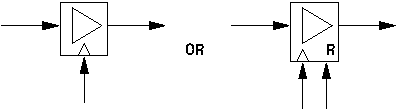
\includegraphics{del}



        \subsection{DFF}

            \subsubsection{purpose}
            
                A D-type flip-flop.

            \subsubsection{arguments}
            
                \begin{tabular}{| l | l |}
                \hline
                Parameters  & Boolean optional initial value \\
                            & integer type of flip-flop \\
                \hline
                Inputs      & data\_in signal, or null \\
                            & clock signal, or null \\
                            & clock enable signal, or null \\
                            & reset, set, clear or preset signal, or null \\
                \hline
                Outputs     & data\_out signal \\
                \hline
                \end{tabular}

            \subsubsection{description}

                This provides a basic D-type flip-flop. Unused arguments may be
                null and unused trailing arguments may be omitted.
                The 2nd argument specifies the type of flip-flop and the
                function of the 4th input signal-\\
                0 - FDRE - R (synchronous reset)\\
                1 - FDSE - S (synchronous set)\\
                2 - FDCE - CLR (asynchronous clear)\\
                3 - FDPE - PRE (asynchronous set)\\
                Any of the 1st (data in), 3rd (clock enable) or 4th
                (reset/set/clear/preset) signal inputs which are unconnectd
                will be connected to GND.
            
            \subsubsection{dump format}
            
                \begin{lstlisting}{gobble=16, language={tde}}
                   DFF {
                    OUT      FDRS622
                    <-
                    D        -
                    C        glob.ruclk
                    CE       -
                    R        OR621
                    S        S601
                   }
                \end{lstlisting}

            \subsubsection{diagrammatic form}

                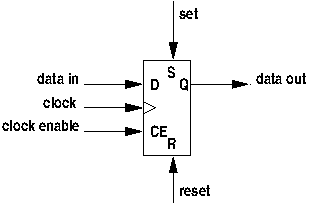
\includegraphics{dff}




        \subsection{DIVERGE}

            \subsubsection{purpose}
            
                A controller for divergent queue signals. Where a queue is read
                within more than one module it is required that each module
                execute a read before the datum is popped. Until all destination
                modules have executed a read the queue must appear unavailable
                for reading to those modules that have already executed a read.
                This is accomplished by inserting this DIVERGE element between
                the queue .NE and .POP signals and the .NE and .POp signals seen
                by the queue reads in each destination module.

            \subsubsection{arguments}
            
                \begin{tabular}{| l | l |}
                \hline
                Parameters  & none \\
                \hline
                Inputs      & clock signal \\
                            & reset signal \\
                            & queue not empty signal \\
                            & module queue pop signal \\
                            & module queue pop signal \\
                            & . \\
                            & . \\
                            & . \\
                \hline
                Outputs     & queue pop signal \\
                            & module queue not empty signal \\
                            & module queue not empty signal \\
                            & . \\
                            & . \\
                            & . \\
                \hline
                \end{tabular}

            \subsubsection{description}

                This splits the source queue .NE (read availability) and .POP
                (acknowledge) signals into a pair per destination module. The
                1st input is the output (read) clock signal for the queue.

                The 2nd input is the .NE (read availability) signal from the queue.
                The 1st output signal is the .POP (acknowledge) signal to the
                queue. The 2nd input is a reset which is asserted if the source
                queue is reset. The 3rd input is the .POP signal from the 1st
                module. The 2nd output is the .NE signal to the 1st module.
                Further input and output signals to other modules may follow. If
                there is only one module the .NE and .POP signals should be just
                connected through. If all destination acknowledge signals go
                high simultaneously the acknowledge signal to the source also
                goes high, otherwise it goes high when the last destination
                acknowledge signal goes high. The destination acknowledge signal
                is high for one clock cycle. When each destination acknowledge
                signal goes high the matching destination availability signal
                will go low at the next clock cycle unless all destination
                modules have also acknowledged in which case destination
                availability signals will be the be the same as the source
                availability signal.

            \subsubsection{dump format}
            
                \begin{lstlisting}{gobble=16, language={tde}}
                       DIVERGE {
                           in:
                               c100
                               S11
                               glob.p.NE
                               S21
                               S30
                           out:
                               glob.p.POP
                               S15
                               S22
                               S31
                       }
                \end{lstlisting}

            \subsubsection{diagrammatic form}

                
\includegraphics{diverge}

 

        \subsection{DOWHILE}

            \subsubsection{purpose}
            
                A {\em do while} statement.

            \subsubsection{arguments}
            
                \begin{tabular}{| l | l |}
                \hline
                Parameters  & none \\
                \hline
                Inputs      & start signal \\
                            & test signal \\
                            & block finish delayed signal \\
                            & optional reset signal or null \\
                            & clock signal \\
                            & optional reset signal or null \\
                \hline
                Outputs     & start signal for the body \\
                            & DO WHILE finish signal \\
                \hline
                \end{tabular}

            \subsubsection{description}

                The start input signal starts the first iteration of the loop by
                propagating straight through to the body start output signal. The
                block finish delayed input signal comes from the block finish
                signal, possibly via an EXECP if the test signal comes from an
                expression containing queue reads. The block finish delayed input
                signal is then routed either through to the body start output
                signal (test succeeds) or via a one cycle delay to the finish
                output signal (test fails).
                
                The optional reset signal clears internal state in the WHILE.

            \subsubsection{dump format}
            
                \begin{lstlisting}{gobble=16, language={tde}}
                   DO WHILE {
                       START_B     S23
                       FINISH      F35
                       <-
                       START       S24
                       TEST        E31[0]
                       CONTIN      F33
                       CLK         glob.c100
                       RESET       s34
                   }
                \end{lstlisting}

            \subsubsection{diagrammatic form}

                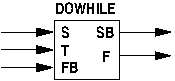
\includegraphics{dowhile}




        \subsection{ELEMENT}

            \subsubsection{purpose}
            
                Create an instance of a netlist element.
                
            \subsubsection{arguments}
            
                \begin{tabular}{| l | l |}
                \hline
                Parameters  & String  the element name               \\
                            & String  netlist block name or null     \\
                            & String    port name         | 1st port \\
                            & integer   port type         |          \\
                            & integer   port width        |          \\
                            & integer   port array format |          \\
                            .                             | 2nd port \\
                            .                                        \\
                \hline
                Inputs      & input 1                                \\
                Inputs      & input 2                                \\
                .                                                    \\
                .                                                    \\
                \hline
                Outputs     & output 1                               \\
                Outputs     & output 2                               \\
                .                                                    \\
                .                                                    \\
                \hline
                \end{tabular}

            \subsubsection{description}

                This is used to explicitly create a component element. It can be
                used to access library components which are not available
                implicitly in normal code or to access external elements such as
                cores. It is useful for accessing hardware elements which are
                peculiar to a particular FPGA rather than being generic.
                Examples of this are Xilinx global clock buffers as these are
                not generic elements normally generated implicitly by the
                compiler.

                The first parameter is the element name. The optional second
                parameter is a netlist identifier for this instance of the
                element. If null an arbitrary identifier of the form "b123" will
                be generated.
                
                The following parameters are quadruples giving the port name,
                port type (0 input, 1 output, 2 3-state output, 4 clock input),
                port width in bits and port array format, 0 for non-array
                ports, 1 for pins as A1, A2, A3 etc. and 2 for EDIF pin arrays.
                For each quadruple there will be an associated signal in the
                input or output list in the order of occurrence in the
                parameter list.
            
            \subsubsection{dump format}
            
                \begin{lstlisting}{gobble=16, language={tde}}
                   ELEMENT DCM block dcm1
                    PIN CLKIN I glob.ruclk
                    PIN CLKFB I prog.cfb
                    PIN CLK0  O prog.cfb_raw
                    PIN CLKDV O prog.pclk_raw
                \end{lstlisting}


        \subsection{EXECP}

            \subsubsection{purpose}
            
                An execution wait for queue availability and/or priority grant.

            \subsubsection{arguments}
            
                \begin{tabular}{| l | l |}
                \hline
                Parameters  & none \\
                \hline
                Inputs      & clock signal \\
                            & start signal \\
                            & buffered queue read/write availability signal \\
                            & unbuffered queue write availability signal \\
                            & unbuffered queue read availability signal \\
                            & priority output signal or null \\
                            & optional reset or null \\
                \hline
                Outputs     & delayed start signal \\
                            & priority input signal or null \\
                            & unbuffered queue write pending signal or null \\
                            & unbuffered queue read pending signal or null \\
                \hline
                \end{tabular}

            \subsubsection{description}
            
                This element delays an execution signal if it is necessary to
                wait for queue availability, for priority or both. The buffered
                queue availability input is high if all associated buffered
                queues to be read or written are available. The unbuffered queue
                availability inputs are similar but the write and read
                availabilities are on separate inputs.
                
                If the queue availability inputs are high and the priority
                encoder passes the signal, the execution signal is passed
                through without delay. If the queue availability inputs are not
                all high or priority has been pre-empted, the execution signal
                is stored until the queue availabilities are high and priority
                is granted at which time a single cycle output pulse is
                generated. An input execution signal must not occur when an
                output is pending however it may occur on the cycle following
                the output pulse. The queue availability inputs may be several
                queue availabilities ANDed together. The reset input, if not
                null, is used to clear any pending execution (waiting on queue
                availability or priority). The pending signals are used to
                notify unbuffered queues that a write or read is pending
                awaiting unbuffered queue availability. It is asserted when the
                start signal is asserted or the registered start signal is
                asserted and all buffered queues are available. The output need
                not have an argument (null) if unbuffered queues are not
                involved.

            \subsubsection{dump format}
            
                The dump format depends on which inputs and outputs
                are used.
            
                \begin{lstlisting}{gobble=16, language={tde}}
                   EXECP {
                        START_DEL SD250
                        PRI_IN    -
                        WPENDING  -
                        RPENDING  -
                        <-
                        CLK       glob.ruclk
                        START_IN  S262
                        BQAV      kandinski.link_0.if_3372.xc2vp_mgt16_0.q1.NF
                        UBQWAV    -
                        UBQRAV    -
                        PRI_OUT   -
                        RESET     -
                   }
                \end{lstlisting}

            \subsubsection{diagrammatic form}

                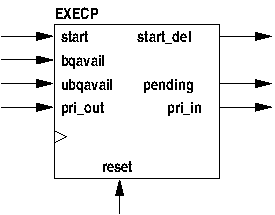
\includegraphics{execp}


            
        \subsection{IBUF}

            \subsubsection{purpose}
            
                A buffered external input signal.

            \subsubsection{arguments}
            
                \begin{tabular}{| l | l |}
                \hline
                Parameters  & String  - optional element identifier \\
                            & String  - input package pin \\
                            & String  - optional input package pin for differential input\\
                            & Boolean - ibufg flag \\
                            & Boolean - differential flag \\
                \hline
                Inputs      & input signal from pad \\
                            & optional differential input signal from pad or null \\
                \hline
                Outputs     & output signal \\
                            & optional differential output signal or null \\
                \hline
                \end{tabular}

            \subsubsection{description}

                This buffers an external input signal. The first parameter
                specifies the ID given to the IBUF element. The second parameter
                gives the primary FPGA pad designation. The third parameter is an
                optional second input pad for differential input or null. The
                fourth parameter is true for an IBUFG or IBUFGDS The last
                parameter is true if the input is differential (IBUFDS, IBUFGDS,
                IBUFDS\_DIFF\_OUT).
                
                There is a primary input signal followed by a second input
                signal if there is differential input to the IBUF
                (IBUFDS, IBUFGDS, IBUFDS\_DIFF\_OUT) or null (IBUF, IBUFG).
                
                There is a primary output signal followed by a second output
                signal if there is differential output from the IBUF
                (IBUFDS\_DIFF\_OUT) or null (IBUF, IBUFG, IBUFDS, IBUFGDS).
                
                There must be a {\bf loc} entry to specify the package pin. For
                differential inputs two consecutive pins are used, positive input
                followed by negative input.

            
            \subsubsection{dump format}
            
                \begin{lstlisting}{gobble=16, language={tde}}
                   IBUF    INPUT327[0] <- PORT_P88 loc=P88, IBUFG
                   IBUF    INPUT430[0] <- PORT_P91, PORT_P92 loc=P91,P92 IBUFDS
                \end{lstlisting}



        \subsection{ILOOP}

            \subsubsection{purpose}
            
                An infinite loop.

            \subsubsection{arguments}
            
                \begin{tabular}{| l | l |}
                \hline
                Parameters  & none \\
                \hline
                Inputs      & start signal \\
                            & block finish signal \\
                \hline
                Outputs     & block start signal \\
                \hline
                \end{tabular}

            \subsubsection{description}
            
                The start input signal is the start signal for all infinite
                loops in this clock domain. The block finish signal is high when
                the last statement in the code block executes. This element
                simply ORs the two inputs.

                Infinite loops containing a single statement that always
                executes in one clock cycle are replaced by a D-flip-flop which
                is set by the clock domain start signal and stays set thereafter
                since the contained statement is to execute on every clock
                cycle.

            \subsubsection{dump format}
            
                \begin{lstlisting}{gobble=16, language={tde}}
                       ILOOP       S12 <- glob.c100.start F14
                \end{lstlisting}

            \subsubsection{diagrammatic form}

                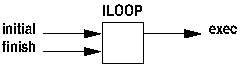
\includegraphics{iloop}






       \subsection{INV}

            \subsubsection{purpose}
            
                An single signal inverter.

            \subsubsection{arguments}
            
                \begin{tabular}{| l | l |}
                \hline
                Parameters  & none \\
                \hline
                Inputs      & input signal \\
                \hline
                Outputs     & output signal \\
                \hline
                \end{tabular}

            \subsubsection{description}
                
                The input and output are single signals, the output being the
                input inverted.

            \subsubsection{dump format}
            
                \begin{lstlisting}{gobble=16, language={tde}}
                       E17[1] = inv(glob.a[1])
                \end{lstlisting}

            \subsubsection{diagrammatic form}

                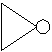
\includegraphics{inv}



        \subsection{OBUF}

            \subsubsection{purpose}
            
                A buffered external output signal.

            \subsubsection{arguments}
            
                \begin{tabular}{| l | l |}
                \hline
                Parameters  & String  - optional array of element identifiers \\
                            & String  - output package pin \\
                            & String  - optional output package pin for differential output\\
                            & boolean - differential flag \\
                \hline
                Inputs      & input signal \\
                            & optional 3-state enable signal (+ve for high-Z) or null\\
                \hline
                Outputs     & output signal to pad \\
                            & optional differential output signal to pad or null \\
                \hline
                \end{tabular}

            \subsubsection{description}

                This buffers an external output signal. The first parameter
                specifies the ID given to the OBUF element. The second parameter
                gives the primary FPGA pad designation. The third parameter is an
                optional second output pad for differential output or null. The
                fourth parameter flags a differential output.
                
                The first input signal is the data input. The second input signal
                is an optional 3-state enable which must be low to drive data onto
                the output pad (OBUFT, OBUFTDS). If this argument is null output
                drive to the pad is continuous (OBUF, OBUFDS).
                
                There is a primary output signal followed by a second output
                signal if there is differential output from the OBUF
                (OBUFDS, OBUFTDS) or null (OBUF, OBUFT).

                There must be a {\bf loc} entry to specify the package pin. For
                differential outputs two consecutive pins are used, positive output
                followed by negative output.

            \subsubsection{dump format}
            
                \begin{lstlisting}{gobble=16, language={tde}}
                   OBUF    PORT_P90 <- OUTPUTBIT213 loc=P90
                   OBUF    PORT_P92 <- OUTPUTBIT412 _EN=T31 loc=P92
                \end{lstlisting}


        \subsection{OPERATOR}

            \subsubsection{purpose}
            
                An arithmetic or logical operator.

            \subsubsection{arguments}
            
                The general form is

                \begin{tabular}{| l | l |}
                \hline
                Parameters  & enumerated type operator code \\
                Parameters  & enumerated type 1st operand type \\
                Parameters  & enumerated type 2nd operand type if binary or ternary \\
                Parameters  & enumerated type 3rd operand type if ternary \\
                Parameters  & enumerated type result type \\
                \hline
                Inputs      & 1st operand array \\
                            & 2nd operand array if binary or ternary \\
                            & 3rd operand array if ternary \\
                \hline
                Outputs     & output array \\
                \hline
                \end{tabular}

                The unused parameters and inputs are missing, not null.

            \subsubsection{description}
                
                Operator codes are -

                \begin{tabular}{| l | l |}
                \hline
                TDEOp.INV    & unary logical inversion \\
                TDEOp.NEG    & unary arithmetic negation \\
                TDEOp.ADD    & binary integer addition \\
                TDEOp.SUB    & binary integer subtraction \\
                TDEOp.ADDSUB & binary integer addition/subtraction \\
                TDEOp.MUL    & binary integer multiplication \\
                TDEOp.DIV    & binary integer division \\
                TDEOp.REM    & binary integer remainder \\
                TDEOp.DIVREM & binary integer division/remainder \\
                TDEOp.EQ     & binary equality test \\
                TDEOp.NE     & binary inequality test \\
                TDEOp.LT     & binary less-than test \\
                TDEOp.LE     & binary less-than-or-equal-to test \\
                TDEOp.GT     & binary greater-than test \\
                TDEOp.GE     & binary greater-than-or-equal-to test \\
                TDEOp.AND    & binary logical and \\
                TDEOp.OR     & binary logical or \\
                TDEOp.XOR    & binary logical exclusive or \\
                TDEOp.LSH    & binary left shift \\
                TDEOp.RSH    & binary right shift \\
                TDEOp.COND   & ternary conditional (\verb'?:') \\
                \hline
                \end{tabular}
                
                Arithmetic operations are either Ptype.UINT (unsigned integer)
                or Ptype.INT (signed integer). These may be mixed. If either
                operand is signed the result will be signed. The width of the
                result is that necessary to retain all significant bits.
                Operands to equality and inequality relational operators
                may be Ptype.UINT, Ptype.INT, Ptype.BITS or Ptype.LOG.
                Operands to the other four relational operators are
                Ptype.UINT or Ptype.INT. The first operand to the shift
                operators may be Ptype.UINT, Ptype.INT or Ptype.BITS. The
                second operand (shift count) must be Ptype.UINT. The shift count
                may be constant or variable. The ternary conditional operator
                first operator must be Ptype.LOG and the other two operands
                must be matching types (may be mixed Ptype.UINT and Ptype.INT)
                and types Ptype.UINT, Ptype.INT, Ptype.BITS or Ptype.LOG.
                
                The integer addition/subtraction operator provides conditional
                addition or subtraction by means of two additional input
                signals. The first selects addition (high) or subtraction (low).
                The second gates the second operand, high for add/subtract
                and low to inhibit add/subtract (output is first operand).
                This operation is available as an inbuilt function, not an
                operator.

                \begin{tabular}{| l | l |}
                \hline
                Parameters  & TDEOp.ADDSUB \\
                Parameters  & enumerated type 1st operand type \\
                Parameters  & enumerated type 2nd operand type \\
                Parameters  & enumerated type result type \\
                \hline
                Inputs      & 1st operand array \\
                            & 2nd operand array \\
                            & add/subtract control (high for add) \\
                            & pass 2nd operand control (2nd operand 0 if this is
                              low) \\
                \hline
                Outputs     & output array \\
                \hline
                \end{tabular}
                
                The integer division/remainder operator produces the quotient and
                remainder in a single division. For the division and remainder
                operators the quotient and remainder are both produced and
                one of these is discarded.
                This operation is available as an inbuilt procedure, not an
                operator.

            \subsubsection{arguments}
            
                \begin{tabular}{| l | l |}
                \hline
                Parameters  & TDEOp.DIVREM \\
                Parameters  & enumerated type 1st operand type \\
                Parameters  & enumerated type 2nd operand type \\
                Parameters  & enumerated type quotient type \\
                Parameters  & enumerated type remainder type \\
                \hline
                Inputs      & 1st operand array \\
                            & 2nd operand array \\
                \hline
                Outputs     & quotient output array \\
                Outputs     & remainder output array \\
                \hline
                \end{tabular}

            \subsubsection{dump format}
            
                \begin{lstlisting}{gobble=16, language={tde}}
                       OP E3[0..8] = E2[0..7] + glob.a[8..15]
                       OP E15[0] = !E14[0]
                       OP E20[0..7] = E4[0] ? blog.a[0..7] : E3[0..7]
                \end{lstlisting}

            \subsubsection{diagrammatic form}

                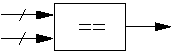
\includegraphics{op}
                
                Example of equality relational operator shown.


        \subsection{OR}

            \subsubsection{purpose}
            
                An OR gate for control signals.

            \subsubsection{arguments}
            
                \begin{tabular}{| l | l |}
                \hline
                Parameters  & none \\
                \hline
                Inputs      & input signal \\
                            & input signal \\
                            & . \\
                            & . \\
                \hline
                Outputs     & AND signal \\
                \hline
                \end{tabular}

            \subsubsection{description}
            
                OR two or more input signals, the result appearing on the
                output.

            \subsubsection{dump format}
            
                \begin{lstlisting}{gobble=16, language={tde}}
                       S11 = A12 | A14 | S8
                \end{lstlisting}

            \subsubsection{diagrammatic form}

                
\includegraphics{or}



        \subsection{PORT}

            \subsubsection{purpose}
            
                Flags a signal which is external to the current source code but
                is not external to the FPGA (i.e. not a pad connection). These
                signals are either connections to an imported core or are
                exported from the current source code which is itself a core.
                
            \subsubsection{arguments}
            
                \begin{tabular}{| l | l |}
                \hline
                Parameters  & Integer type of signal \\
                            & string  port name \\
                \hline
                Inputs      & signal or signal array \\
                \hline
                Outputs     & none \\
                \hline
                \end{tabular}

            \subsubsection{description}

                 The first parameter is an integer type code for the port type
                 which is 0 for input, 1 for output or 2 for 3-state output.
                 The second parameter is the port name.
            
            \subsubsection{dump format}
            
                \begin{lstlisting}{gobble=16, language={tde}}
                   PORT {
                       par:
                           Str     O
                           Int     ADDRESS
                       in:
                           Var     glob.addr[0..18]
                   }
                \end{lstlisting}



        \subsection{PRIORITY}

            \subsubsection{purpose}
            
                A priority encoder.

            \subsubsection{arguments}
            
                \begin{tabular}{| l | l |}
                \hline
                Parameters  & none \\
                \hline
                Inputs      & input signal 0 \\
                            & input signal 1 \\
                            & . \\
                            & . \\
                \hline
                Outputs     & output signal 0 \\
                            & output signal 1 \\
                            & . \\
                            & . \\
                \hline
                \end{tabular}

            \subsubsection{description}

            When one or more inputs are high the highest priority matching
            output signal will be high and all other outputs low. The inputs are
            ordered in decreasing priority (the 1st is highest).

            The number of outputs is equal to the number of inputs or the
            number of inputs + 1. In the latter case the last output is
            the 'else' case, i.e. no inputs high.

            \subsubsection{dump format}
            
                \begin{lstlisting}{gobble=16, language={tde}}
                   PRIORITY {
                    OUT   PRI_OUT40234[0,1,2,3,4]
                    ELSE  kandinski.processing_0.timer_0.mutex_var_0.pri.PE[0]
                    <-
                    IN    tPRI_IN40233[0,1,2,3,4]
                   }
                \end{lstlisting}

            \subsubsection{diagrammatic form}

                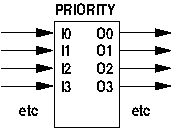
\includegraphics{priority}



        \subsection{QUEUEBUFFER}

            \subsubsection{purpose}
            
                A queue buffer.

            \subsubsection{arguments}
            
                \begin{tabular}{| l | l |}
                \hline
                Parameters  & Integer depth \\
                            & Boolean use hardware FIFO is possible, or null \\
                            & String initial value (hexadecimal string) or null \\
                \hline
                Inputs      & input clock signal, or null if same as output clock \\
                            & output clock signal \\
                            & input data array \\
                            & push datum signal (.PUSH) \\
                            & pop datum signal (.POP) \\
                            & reset signal (optional) \\
                \hline
                Outputs     & output data array                          \\
                            & read available signal (.NE - not empty)  \\
                            & write available signal (.NF - not full)    \\
                            & ready availability signal for unbuffered queue \\
                            & synchronous buffer occupancy count or null \\
                            & synchronous buffer space count or null     \\
                            & asynchronous buffer write status           \\
                            & asynchronous buffer read status            \\
                            & reset signal (optional) \\
                \hline
                \end{tabular}

            \subsubsection{description}

                A normal queue buffer has a depth of 2. If the depth is > 2, an
                initial value is not allowed. If a separate input clock is
                supplied, depths start at 16 and are various powers of 2
                depending on the size ranges of the block RAMs in the particular
                FPGA. If the input data array and output data array arguments
                are null then this is a null data queue buffer and the buffer
                depth is a power of 2 greater than 3.
                
                The 2nd output signal is the read availability signal. This is
                high if the buffered queue is not empty. For an unbuffered queue
                it is high if the queue is waiting on a write, i.e. it is
                connected to the PUSH input.
                
                The 3rd output signal is the write availability signal. This is
                high if the buffered queue is not full. For an unbuffered queue
                it is high if the queue is waiting on a read, i.e. it is
                connected to the POP input.
                
                The 4th output is null for a buffered queue. For an unbuffered
                queue it is the AND of the push (write) and pop (read) inputs
                (which is also the AND of the read availability (NE) and write
                availability (NF) signals.

                If the 5th output is not null this gives the number of words in
                a synchronous queue buffer synchronised to the queue clock (read
                and write).

                If the 6th output is not null this gives the number of free
                spaces in a synchronous queue buffer synchronised to the queue
                clock (read and write).

                If the 7th output is not null this gives the buffer status for
                an asynchronous queue buffer synchronised to the write (input)
                clock.

                If the 8th output is not null this gives the buffer status for
                an asynchronous queue buffer synchronised to the read (output)
                clock.

                If there is an 9th output this is a reset signal. This
                signal goes high for one clock cycle when the queuebuffer is
                reset via the reset() inbuilt procedure. For an asynchronous
                queuebuffer this signal is synchronised to the read (output)
                clock and is timed to follow the reset of the input (write)
                side of the queuebuffer.
            
                The asynchronous queue buffer status is a 5-bit word
                whose bits are -
                
                \begin{tabular}{| l | l |}
                \hline
                bit 0 & not full                        \\ \hline
                bit 1 & empty to 1/4 full + 1           \\ \hline
                bit 2 & 2 words to 1/2 full  + 1        \\ \hline
                bit 3 & 1/4 full + 1 to 3/4 full  + 1   \\ \hline
                bit 4 & 1/2 full + 1 to full            \\ \hline 
                bit 5 & 3/4 full + 1 to full            \\ \hline  
                \end{tabular}
                
                The bits are mutually exclusive and one of them is always set.
            
                Synchronous data queue buffers have a default depth of 2.
                Synchronous null queue buffers have a default depth of 16.
                Asynchronous data queue buffers have a default depth of 16.
                Asynchronous null queue buffers have a default depth of 16. Null
                queue buffers may have a depth which is 4 or greater and which is
                a power of 2. Data queue buffers may have the following depths -
                \blist
                \item   Spartan2, Virtex - 16, 256, 512, 1024, 2048 or 4096
                \item   Spartan3, Virtex2, Virtex2Pro, Virtex4 - 16, 512, 1024, 2048, 4096, 8192 or 16384
                \item   Virtex-5 - 64, 1024, 2048, 4096, 8192, 16384 or 32768
                \blend
                and for synchronous buffers depth 2 is also allowed and is
                the default.
                
                For queues of depth zero the signals have rather different
                meanings -
                \blist
                \item   PUSH - unbuffered queue write is pending from an EXECP
                \item   NE - connected to PUSH
                \item   POP - unbuffered queue read is pending from an EXECP
                \item   NF - connected to POP
                \blend
                outputs NE and NF simply reflect the PUSH and POP inputs. These
                are ANDed together to form an unbuffered queue availability
                signal (ready) back to the relevant EXECPs to synchronise the
                write/read pair.
                

            \subsubsection{dump format}
            
                \begin{lstlisting}{gobble=16, language={tde}}
                   QUEUEBUFFER  depth 2 {
                    OUT      kandinski.dps[0..11,12..21,22..30]
                    NE       kandinski.dps.NE
                    NF       kandinski.dps.NF
                    CNT      -
                    SPC      -
                    WSTAT    -
                    RSTAT    -
                    <-
                    CLKIN    -
                    CLKOUT   glob.ruclk
                    DATA     kandinski.dps.D[0..11,12..21,22..30]
                    PUSH     S5669
                    POP      SD5715
                    RESET    GND
                   }
                \end{lstlisting}
                
                The minimum size of the buffer is two and this is implemented as
                two registers. {\bf NF} stands for "Not Full", meaning
                that at least one free register is available for writing. {\bf
                PUSH} is ""push data onto queue". {\bf NE}
                stands for "Not Empty, meaning one or more registers contains
                data which can be read. {\bf POP} acknowledges a read, popping
                the word from the buffer (queue).
                
                Where a queue depth of zero is specified the "queue" is
                unbuffered. In that case this QUEUEBUFFER element simply
                connects OUT to DATA, NE to PUSH and NF to POP and there is no
                included logic. PUSH is now a write pending signal and POP
                a read pending signal. NE and NF are ANDed to form the unbuffered
                queue availability signal to both the read and write EXECP
                elements involved.

            \subsubsection{diagrammatic form}

                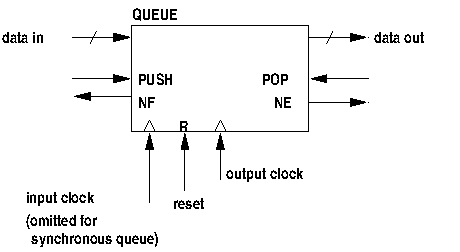
\includegraphics{queue}
                
                Buffer word and space counts and status outputs not shown.




        \subsection{REG}

            \subsubsection{purpose}
            
                A register (static variable).

            \subsubsection{arguments}
            
                \begin{tabular}{| l | l |}
                \hline
                Parameters  & String[] - block ids \\
                            & String - initial value \\
                            & boolean - IOB flag \\
                            & boolean - DSP flag \\
                \hline
                Inputs      & clock signal (may be null if .D null) \\
                            & data signal array (.D - may be null) \\
                            & clock enable signal or signal array (.CE) \\
                            & set/reset signal or signal array (.RES) \\
                \hline
                Outputs     & data signal array \\
                \hline
                \end{tabular}
                
                The block IDs are the identifiers for the DFF elements comprising
                the register, from LSB to MSB. The IOB flag indicates that the DFFs
                within I/O blocks should be used. This applies when the register
                input is connected to input buffers our its output is connected to
                output buffers. The DSP flag indicates that a DSP block may be used
                to implement the register instead of using CLB flip-flops.
                
                The either or both the clock enable and reset inputs may be
                single signals in which case they will be connected across all
                bits.

            \subsubsection{description}

                When the clock enable is high data will be clocked in on the next
                clock edge. For a primitive type all clock enable inputs are tied
                together as are all reset inputs. For a compound type clock enables
                and resets are grouped in words corresponding to primitives. The
                resets return the state to the initial value (0 by default). If the
                clock is null, there are no inputs to this register so generate a
                constant instead.


            \subsubsection{dump format}
            
                \begin{lstlisting}{gobble=16, language={tde}}
                       REG
                           OUT  glob.v[0..7]
                           <-
                           CLK  glob.c100
                           DATA glob.v.D[0..7]
                           CE   glob.v.CE[0..7]
                           R    glob.v.RES[0..7]
                           {0x0}{tnm=reg1}
                \end{lstlisting}
                The last line shows the initial value folowed by any flags.

            \subsubsection{diagrammatic form}

                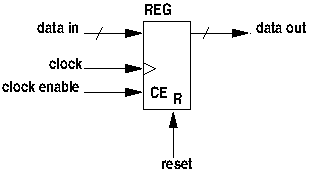
\includegraphics{reg}
                
                This only shows one word of a multiword register. Although
                they share a common identifier, the words of a register
                of compound type (array or struct) are independent. The data
                input and output will be labelled with the associated subscript
                range.


        \subsection{RESYNC}

            \subsubsection{purpose}
            
                A pulse or level resynchroniser.

            \subsubsection{arguments}
            
                \begin{tabular}{| l | l |}
                \hline
                Parameters  & none \\
                \hline
                Inputs      & input signal \\
                            & input clock signal \\
                            & output clock signal \\
                \hline
                Outputs     & output signal \\
                \hline
                \end{tabular}

            \subsubsection{description}

                The input may be a pulse or a level. When the input rises the
                rise is captured by the next input clock edge and an output
                pulse of one period duration is generated on the next output
                clock edge.

            \subsubsection{dump format}
            
                \begin{lstlisting}{gobble=16, language={tde}}
                   RESYNC {
                       in:
                           glob.a[0]
                           glob.c100
                           glob.bus_clk
                       out:
                           E41[0]
                   }
                \end{lstlisting}

            \subsubsection{diagrammatic form}

                
\includegraphics{resync}



        \subsection{RRAM}

            \subsubsection{purpose}
            
                Registered-output RAM.

            \subsubsection{arguments}
            
                \begin{tabular}{| l | l |}
                \hline
                Parameters  & Integer number of ports \\
                            & Integer data width in bits \\
                            & Integer address width in bits \\
                            & String[] optional initialisation or null \\
                            & String optional output register 0 string initial hex value, or null \\
                            & String optional output register 1 string initial hex value, or null \\
                            & String - attribute key \\
                            & String - data for attribute key \\
                            &       ...     other attribute pairs \\
                \hline
                Inputs      & clock signal, port0 \\
                            & address array, port0 \\
                            & data\_in array, or null, port0 \\
                            & read signal, or null, port0 \\
                            & write signal, or null, port0 \\
                            & clock signal, port1 \\
                            & address array, port1 \\
                            & data\_in array, or null, port1 \\
                            & read signal, or null, port1 \\
                            & write signal, or null, port1 \\
                            & ..etc.. \\
                \hline
                Outputs     & data\_out array, or null, port0 \\
                            & data\_out array, or null, port1 \\
                \hline
                \end{tabular}

            \subsubsection{description}

                This is a RAM with clocked read and write. The output for a port
                reflects the memory contents following a read clock cycle.

                The 2nd parameter gives the data width and the address width
                gives the memory depth (number of words). All port addresses
                must be the same width and all port data inputs and outputs must
                be the same width. The initialisation string array has one entry
                for each initial value. Each entry is a hexadecimal string. The
                initialisation array may be smaller than the depth of the RAM
                but not larger. The initialisation parameter may be omitted in
                which case the RAM is explicitly initialised to all 0. Ports
                which are not written have null arguments for the data in and
                the write enable. Ports which are not read have null arguments
                for the data out.

                For Xilinx FPGAs registered-output RAM is block RAM. The address
                width is limited to a maximum of 12 bits (a depth of 4096 words)
                for Spartan 2, Virtex and  Virtex E and 14 bits (a depth of
                16384 words) for Spartan 3, Virtex 2 and Virtex 2 PRO. The data
                width is not limited.
                
                Attributes are -
                \begin{tabular}{| l | l |}
                \hline
                loc             & block RAM location \\
                tnm             & timing group name \\
                writemode       & write mode \\
                writemodea      & port A write mode \\
                writemodeb      & port B write mode \\
                continuous      & continuous enable \\           
                \hline
                \end{tabular}
                There is one {\bf loc} attribute per block. Block RAM formats
                are selected by address width, then the number of blocks is
                determined by the total data width divided by the block data width.
                Block locations are in order from the least significant data bits.
                The other attributes are be applied to each
                individual RAMB4\_S, RAMB4\_S\_S, RAMB16\_S or
                RAMB16\_S\_S prepended in each case with "INST name "
                where 'name' is the generated netlist identifier for the
                RAM component.

            \subsubsection{dump format}
            
                \begin{lstlisting}{gobble=16, language={tde}}
                   RRAM - 2 ports {
                    OUT0	kandinski.link_0.if_3372.xc2vp_mgt16_0.crcunblock_0.buf_0[0..31,32]
                    OUT1	kandinski.link_0.if_3372.xc2vp_mgt16_0.crcunblock_0.buf_1[0..31,32]
                    <-
                    CLK0	glob.ruclk
                    ADDR0	MADDR1031[0..5]
                    DATA0	MDATA1032[0..31,32]
                    RE0	-
                    WE0	S1057
                    CLK1	glob.ruclk
                    ADDR1	S38113[0..5]
                    DATA1	-
                    RE1	S38114
                    WE1	-
                       initialised
                   }
                \end{lstlisting}
                
                The presence of an initialisation argument is flagged
                but the values are not listed.

            \subsubsection{diagrammatic form}

                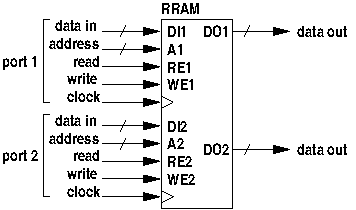
\includegraphics{rram}


        \subsection{SAMPLE}

            \subsubsection{purpose}
            
                Sample data from a different clock domain.

            \subsubsection{arguments}
            
                \begin{tabular}{| l | l |}
                \hline
                Parameters  & Boolean input clock freq > output clock freq \\
                \hline
                Inputs      & input data array \\
                            & input clock signal \\
                            & output clock signal \\
                \hline
                Outputs     & output data array \\
                \hline
                \end{tabular}

            \subsubsection{description}

                The input is sampled into the output clock domain. However, sampled
                data will not be corrupted depending on the relative
                clock rates data may be missed or multiply sampled. The input
                may be a different size to the output, zero padding or
                truncation being applied as required.

            \subsubsection{dump format}
            
                \begin{lstlisting}{gobble=16, language={tde}}
                   SAMPLE {
                       params:
                           true
                       in:
                           glob.a[0..7]
                           glob.c100
                           glob.bus_clk
                       out:
                           E41[0..7]
                   }
                \end{lstlisting}


        \subsection{SELECT}

            \subsubsection{purpose}
            
                Select one of several inputs.

            \subsubsection{arguments}
            
                \begin{tabular}{| l | l |}
                \hline
                Parameters  & String - unselected output value \\
                            & boolean - ALU flag \\
                            & boolean - DSP flag \\
                \hline
                Inputs      & select signal \\
                            & signal array \\
                            & select signal \\
                            & signal array \\
                            & . \\
                            & . \\
                            & . \\
                \hline
                Outputs     & signal array \\
                \hline
                \end{tabular}

            \subsubsection{description}

                The inputs are in pairs. The first of each pair is an
                input signal which selects the second of the pair (a signal
                array) to be connected to the output signal array. If no
                select signals are high the output is explicitly zero.
                The input arrays may be smaller than the output array.
                
                The data inputs may be narrower than the output in which case
                they will be padded or sign extended as appropriate.
                
                SELECT TDEs with only a single select/data input pair will be
                optimised away (data input connoected to output) unless the
                output is a queue variable which is not primitive. In that special
                case the SELECT TDE functions as a gate to ensure that a field
                or array member of a queue that is not explicitly assigned when
                the queue as a whole is assigned is assigned zero/false.

            \subsubsection{dump format}
            
                \begin{lstlisting}{gobble=16, language={tde}}
                       SELECT {
                           par:
                           in:
                               S11
                               glob.a[0..7]
                               S15
                               glob.b[24..31]
                           out:
                               glob.c[0..7]
                       }
                \end{lstlisting}

            \subsubsection{diagrammatic form}

                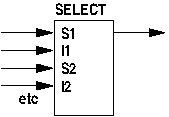
\includegraphics{select}


        \subsection{SIG}

            \subsubsection{purpose}
            
                Declare a signal or signal array.

            \subsubsection{arguments}
            
                \begin{tabular}{| l | l |}
                \hline
                Parameters  & none \\
                \hline
                Inputs      & signal or signal array \\
                            & signal or signal array \\
                            & . \\
                            & . \\
                \hline
                Outputs     & none \\
                \hline
                \end{tabular}

            \subsubsection{description}

                There may be any number of inputs. Each input
                may be a single signal or an array. Declarations
                are created which will be dimensioned if arrays.
                
                This element is only used by the simulator, not the code
                generator. It is not generated unless the -s or -T options
                are passed to the compiler.

            \subsubsection{dump format}
            
                \begin{lstlisting}{gobble=16, language={tde}}
                       SIG     glob.a
                       SIG     E1[1]
                       SIG     S11
                       SIG     mod1_1.a[8]
                \end{lstlisting}


%        \subsection{SIMREAD}
%
%            \subsubsection{purpose}
%            
%                Read a line from a file during simulation.
%
%            \subsubsection{arguments}
%            
%                \begin{tabular}{| l | l |}
%                \hline
%                Parameters  & string  file path name \\
%                \hline
%                Inputs      & clock signal \\
%                            & execution signal for the read \\
%                \hline
%                Outputs     & signal array driven from input data line \\
%                            & \ldots \\
%                            & \ldots \\
%                \hline
%                \end{tabular}
%
%            \subsubsection{description}
%
%                This element is only used by the simulator, not the code
%                generator. It is not generated unless the -s option
%                is passed to the compiler.
%                When the 2nd input signal is high, one line is read from the
%                file, is decoded according to the type of the output signal
%                arrays and the outputs are driven using the decoded values.
%                
%            
%            \subsubsection{dump format}
%            
%                This element is not printed.
%
%
%        \subsection{SIMWRITE}
%
%            \subsubsection{purpose}
%            
%                Write a line to a file during simulation.
%
%            \subsubsection{arguments}
%            
%                \begin{tabular}{| l | l |}
%                \hline
%                Parameters  & string  file path name \\
%                \hline
%                Inputs      & clock signal \\
%                            & execution signal for the write \\
%                            & signal array to be written to the data line \\
%                            & \ldots \\
%                            & \ldots \\
%                \hline
%                Outputs     & none \\
%                \hline
%                \end{tabular}
%
%            \subsubsection{description}
%
%                This element is only used by the simulator, not the code
%                generator. It is not generated unless the -s option
%                is passed to the compiler.
%                When the 2nd input signal is high, one line is written to the
%                file, each input signal array contributing one number to the
%                line.
%            
%            \subsubsection{dump format}
%            
%                This element is not printed.
%
%        \subsection{SIMVAR}
%
%            \subsubsection{purpose}
%            
%                A variable reference (only used by the simulator).
%
%            \subsubsection{arguments}
%            
%                \begin{tabular}{| l | l |}
%                \hline
%                Parameters  & Var class  variable \\
%                \hline
%                Inputs      & none \\
%                \hline
%                Outputs     & none \\
%                \hline
%                \end{tabular}
%
%            \subsubsection{description}
%
%                If the simulator is being used one of these elements is placed
%                on the list for every target variable.
%            
%            \subsubsection{dump format}
%            
%                This element is not printed.
%



        \subsection{SPECIAL}

            \subsubsection{purpose}
            
                Provides special functions, perhaps vendor specific.
                
            \subsubsection{arguments}
            
                \begin{tabular}{| l | l |}
                \hline
                Parameters  & Integer type of special function \\
                \hline
                Inputs      & \ldots \\
                \hline
                Outputs     & \ldots \\
                \hline
                \end{tabular}

            \subsubsection{description}

                 The first parameter is an integer type code which selects the
                 particular special function. At the moment there are only two
                 special functions.

                {\bf add line to the NCF or the XDC file}

                \begin{tabular}{| l | l |}
                \hline
                Parameters  & Integer 0 or 1 \\
                            & String  a format string \\
                \hline
                Inputs:     & signal  optional signal \\
                            & . \\
                            & . \\
                \hline
                Outputs:    & none \\
                \hline
                \end{tabular}

                The format string is written to the ISE NCF file or the Vivado
                XDC file. The format string may contain \%n or \%N conversions
                at which points netlist identifiers are to be inserted. The
                netlist identifiers are obtained from the input signals which
                are matched to the conversions in order. There will usually be
                at most one of these though the format allows any number. \%n is
                replaced by the identifier of the next input signal argument.
                \%N is similar to the above but changes the identifier to upper
                case and removes any leading "GLOB\_" string  This is used for
                generating clock timing group names from the clock signal
                identifier.

        \subsection{START}

            \subsubsection{purpose}
            
                Start an execution stream.

            \subsubsection{arguments}
            
                \begin{tabular}{| l | l |}
                \hline
                Parameters  & none \\
                \hline
                Inputs      & start level signal (may be VCC)\\
                            & domain clock signal \\
                \hline
                Outputs     & start pulse signal \\
                \hline
                \end{tabular}

            \subsubsection{description}

                The start input may be a pulse or a level. When the start signal
                rises the rise is captured by the next clock edge and an
                output pulse of one period duration is generated on the next
                clock edge. The logic is locked after this pulse so that
                any further start signal rises are ignored. The
                start level signal may be VCC if execution is to start
                immediately after configuration loading, otherwise it must be
                derived combinatorially from external inputs.

            \subsubsection{dump format}
            
                \begin{lstlisting}{gobble=16, language={tde}}
                   START { 
                    OUT  glob.uclk.start
                    <-
                    IN   VCC
                    COUT glob.uclk
                   }
                \end{lstlisting}

            \subsubsection{diagrammatic form}

                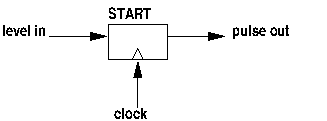
\includegraphics{start}


        \subsection{TSELECT}

            \subsubsection{purpose}
            
                A 3-state driver.

            \subsubsection{arguments}
            
                \begin{tabular}{| l | l |}
                \hline
                Parameters  & none \\
                \hline
                Inputs      & select signal \\
                            & signal array \\
                \hline
                Outputs     & signal array \\
                \hline
                \end{tabular}

            \subsubsection{description}

                The first of each input is a source signal array to be
                conditionally connected to the output signal array.
                The second input is an enable signal. When the enable is
                high the output is driven by the input. When the enable
                is low the output is not driven (is high impedance).
                The input array and output array must be the same size.

            \subsubsection{dump format}
            
                \begin{lstlisting}{gobble=16, language={tde}}
                       TSELECT {
                           par:
                           in:
                               glob.a[0..7]
                               S11
                           out:
                               glob.c[0..7]
                       }
                \end{lstlisting}


        \subsection{WAIT}

            \subsubsection{purpose}
            
                A parallel block completion wait.

            \subsubsection{arguments}
            
                \begin{tabular}{| l | l |}
                \hline
                Parameters  & none \\
                \hline
                Inputs      & clock signal \\
                            & reset signal or null \\
                            & input signal \\
                            & . \\
                            & . \\
                            & . \\
                \hline
                Outputs     & output signal \\
                \hline
                \end{tabular}

            \subsubsection{description}

                There are four or more inputs. The first input signal is the clock
                signal for the clock domain. The second input signal is a reset
                signal or is null if there is no reset. The third and following are
                finish signals. If all input signals go high simultaneously the
                output signal also goes high, otherwise the output signal goes high
                when the last input signal goes high. The output signal is high for
                one clock cycle. The reset input clears any pending latched
                completion signals.

            \subsubsection{dump format}
            
                \begin{lstlisting}{gobble=16, language={tde}}
                       WAIT {
                           in:
                               c100
                               null
                               S11
                               S13
                           out:
                               S15
                       }
                \end{lstlisting}

            \subsubsection{diagrammatic form}

                
\includegraphics{wait}


        \subsection{WHEN}

            \subsubsection{purpose}
            
                A {\em when} statement.

            \subsubsection{arguments}
            
                \begin{tabular}{| l | l |}
                \hline
                Parameters  & none \\
                \hline
                Inputs      & start signal \\
                            & test signal \\
                            & true block finish signal or null \\
                            & false block finish signal or null \\
                \hline
                Outputs     & true block start signal \\
                            & false block start signal \\
                            & WHEN finish signal or null \\
                \hline
                \end{tabular}

            \subsubsection{description}

                A start signal will be routed to either the true block start
                output or the false block start output according to whether the
                test input signal is high or low. The finish signals for the
                true and false blocks are returned as inputs and the OR of these
                emerges as the third output, signalling the end of the
                statement.

                A missing true or false block will have the block start signal
                connected back to the associated block finish signal via a
                1-cycle delay (TDEType.DEL). If both the true block and the
                false block require a single DEL for their finish signals these
                will be optimised to a separate common DEL from the start signal
                to the finish signal. In that case -
                \blist
                \item   true block finish signal
                \item   false block finish signal
                \item   WHEN finish signal
                \blend
                arguments to the WHEN will all be null.

            \subsubsection{dump format}
            
                \begin{lstlisting}{gobble=16, language={tde}}
                   WHEN {
                    T_START  S307
                    F_START  FS270
                    FINISH   F268
                    <-
                    START    S267
                    TEST     E274[0]
                    T_FINISH F281
                    F_FINISH FF312
                   }
                \end{lstlisting}

            \subsubsection{diagrammatic form}

                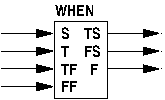
\includegraphics{when}

        \subsection{WHILE}

            \subsubsection{purpose}
            
                A {\em while} statement.

            \subsubsection{arguments}
            
                \begin{tabular}{| l | l |}
                \hline
                Parameters  & none \\
                \hline
                Inputs      & start signal \\
                            & test signal \\
                            & continuation signal from the body \\
                            & clock signal \\
                            & optional reset signal or null \\
                \hline
                Outputs     & start signal for the body \\
                            & WHILE finish signal \\
                \hline
                \end{tabular}

            \subsubsection{description}
            
            If the test input signal is high when start input signal goes high,
            the latter is routed to the body start output signal to execute the
            contained code block. If the test input signal is low when start
            input signal goes high, the latter is delayed by one clock cycle and
            then appears on the finish output signal (i.e. a {\em while} takes a
            minimum of one clock cycle). When the body code block finishes the
            last execution signal comes back to the continuation input signal.
            If the test input signal is high the continuation input signal is
            routed to the body start output signal to again execute the
            contained code block. If the test input signal is low the
            continuation input signal is routed through to the finish output
            signal, again with one clock cycle delay.

            The start signal and the continuation signal may come from
            EXECP elements which wait on queue availability in the test value.
                
            The optional reset signal clears internal state in the WHILE.

            \subsubsection{dump format}
            
                \begin{lstlisting}{gobble=16, language={tde}}
                   WHILE {
                    START_B    S505
                    FINISH     S516
                    <-
                    START      S502
                    TEST       E504[0]
                    CONTIN     F507
                    C          glob.ruclk
                    RESET      null
                   }
                \end{lstlisting}

            \subsubsection{diagrammatic form}

                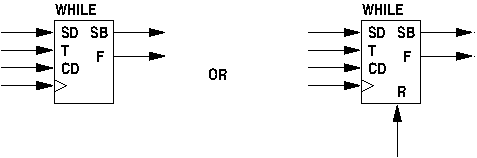
\includegraphics{while}


        \subsection{XOR}

            \subsubsection{purpose}
            
                An XOR gate for control signals.

            \subsubsection{arguments}
            
                \begin{tabular}{| l | l |}
                \hline
                Parameters  & none \\
                \hline
                Inputs      & input signal \\
                            & input signal \\
                            & . \\
                            & . \\
                \hline
                Outputs     & AND signal \\
                \hline
                \end{tabular}

            \subsubsection{description}
            
                Exclusive OR two or more input signals, the result appearing
                on the output.

            \subsubsection{dump format}
            
                \begin{lstlisting}{gobble=16, language={tde}}
                       S11 = A12 ^ A14 ^ S8
                \end{lstlisting}

            \subsubsection{diagrammatic form}

                
\includegraphics{xor}










    \section{Intermediate code optimisation}
        
        The intermediate code list is optimised by repeated applications of
        the following -
        \blist
        \item   Combine any {\bf EXECP}s with a common start and identical avail
                signal.
        \item   Combine any parallel {\bf DEL}s with a common start
                driving a common {\bf WAIT}.
        \item   Eliminate any {\bf DEL} in parallel with one or more EXECPs with
                a common start driving a common WAIT.
        \item   Eliminate any {\bf WAIT} that has a single input.
        \item   Eliminate any duplicate {\bf SELECT} inputs.
        \item   Find any AND or OR gates which have duplicated inputs
                and remove the duplicates. If this results in a single
                input remaining, eliminate the gate and connect
                the input to the output.
        \item   Find any {\bf INV}s with GND or VCC input and eliminate
                them, connecting the output to the inverse of the constant
                input.
        \item   Find any nested {\bf AND}, {\bf OR} or {\bf XOR} gates and
                consolidate them.
        \item   Find any control (not source code) {\bf AND} or {\bf OR} gates
                whose outputs are not connected and eliminate them.
        \item   Find any {\bf DEL}s whose outputs are not connected and
                eliminate them.
        \item   Find any WHENs which have a single {\bf DEL} in both the true
                block and the false block. Remove these and instead connect a
                single DEL from the start input to both the true block finish
                input and the false block finish input. This will result in
                an OR with identical inputs which will be eliminated by
                another optimisation iteration.
        \item   Eliminate any {\bf ILOOP}s which have the same output start
                signal and input finish signal. These infinite loops are
                empty, probably because they contain only value equivalence
                statements.
        \item   Find any {\bf ILOOP}s which have a single {\bf DEL} from the
                output start signal to the input finish signal. Replace the
                pair with a DFF whose SET input is driven by the start signal.
        \item   Find multiple {\bf DFF}s driven by a common {\bf START} and
                eliminate all but one.
        \item   Find any branch statements in which all branches, including
                the default, have a single DEL. Remove all the DELs and the
                final associated OR and replace with a single DEL from the
                start signal.
        \blend
        These optimisations are repeatedly applied to the list until a pass
        makes no change.


    \section{Intermediate code examples}

        % set frames for all further listings
        \lstset{
            basicstyle=\footnotesize\ttfamily,
            basewidth={0.5em},
            frame=single
        }
    
        Note that in the following examples the intermediate code dumps and the
        associated diagrams only show sections of the logic that illustrate the
        points under discussion - they are not complete listings or diagrams.
        
        In many cases clock inputs are not shown. The examples are constructed
        to use clock {\bf c100} and this can be assumed unless shown otherwise.
        
        In all the examples the signal {\bf glob.c100.start} appears. This is
        a single cycle pulse, synchronised to the {\bf c100} 100MHz clock, which
        is distributes to all execution threads to initiate them. In practice
        a recent change to the compiler has inserted a single cycle delay
        between this signal and every thread that it initiates but this is not
        shown in the examples. The purpose of the extra cycle is simply to avoid
        the path delays associated with distributing {\bf glob.c100.start} which
        can have a very high fanout. The inserted flip-flop in the path to each
        thread will be placed close the the logic that it initiates resulting
        in a much shorter path into the thread. {\bf glob.c100.start} will still
        have a high fanout but there is no combinatorial logic between its
        source and the myriad destination flip-flops.
    
        \subsection{top level sequential block}

            The code -
            \begin{lstlisting}[gobble=12, language=threepl]
               module "csiro/hymod/io1.3pl"

               useclock(c100);

               static({s1, s2}, "uint:8");

               seq {
                   s1 <- s2;
                   s2 <- s1;
               }
            \end{lstlisting}
            contains one execution thread. That thread will be an infinite loop
            containing two executable statements. The assignments do not wait on
            queues. The intermediate code would look like -
            \begin{lstlisting}{gobble=12, language={tde}}
               DEL F14 <- (1) glob.c100 S13
               DEL F17 <- (1) glob.c100 F14
               ILOOP       S13 <- glob.c100.start F17
               START       glob.c100.start <- START=VCC, CLK=glob.c100
               glob.s1.CE[0..7] = S13
               glob.s1.D[0..7] = glob.s2[0..7]
               glob.s1.RES[0..7] = GND
               REG
                   OUT  glob.s1[0..7]
                   <-
                   CLK  glob.c100
                   DATA glob.s1.D[0..7]
                   CE   glob.s1.CE[0..7]
                   R    glob.s1.RES[0..7]
                   {0x00}
               glob.s2.CE[0..7] = F14
               glob.s2.D[0..7] = glob.s1[0..7]
               glob.s2.RES[0..7] = GND
               REG
                   OUT  glob.s2[0..7]
                   <-
                   CLK  glob.c100
                   DATA glob.s2.D[0..7]
                   CE   glob.s2.CE[0..7]
                   R    glob.s2.RES[0..7]
                   {0x00}
            \end{lstlisting}
            The multiple versions of value variable {\bf start} (created
            in header code csiro/hymod/io1.3pl) are a result of the internal
            intricacies of the compiler. The last value the variable contains
            is assigned to the unappended identifier {\bf glob.start}
            in an attempt to provide a useful value in simulation (no longer
            enabled).

            Diagrammatically this is -

            
\includegraphics{e1}
            
            The thread is started from signal {\bf VCC} so element START generates
            a single pulse using clock {\bf c100}. This is injected into
            {\bf ILOOP} to start the infinite loop. The execution signal for the
            body of the infinite loop is {\bf S13}. The loop body is a {\bf seq}
            block containing two statements. The first is executed by {\bf S13} and
            a finish signal is generated one clock cycle later ({\bf F14}. This
            finish signal is the start signal for the next statement. A finish
            signal is generated one clock cycle later for the second statement
            ({\bf F17}). This second finish signal marks the completion of the loop
            body code so it is fed back to the {\bf ILOOP} to generate the next
            iteration. There is no delay in {\bf ILOOP} (it is simply an OR gate)
            so the loop executes every two clock cycles.

            The two execute signals, {\bf S13} and {\bf F14} control the
            assignments to the two static variables {\bf s1} and {\bf s2} via their
            CE inputs.

        \subsection{top level static assignment}
        
            If we simplify the above code so that the infinite loop contains
            only a single assignment -
            \begin{lstlisting}[gobble=12, language=threepl]
               static({s1, s2}, "uint:8");

               s1 <- s2;
            \end{lstlisting}
            then the intermediate code is -
            \begin{lstlisting}{gobble=12, language={tde}}
               START       glob.c100.start <- START=VCC, CLK=glob.c100
               glob.s1.CE[0..7] = S11
               glob.s1.D[0..7] = glob.s2[0..7]
               glob.s1.RES[0..7] = GND
               REG
                   OUT  glob.s1[0..7]
                   <-
                   CLK  glob.c100
                   DATA glob.s1.D[0..7]
                   CE   glob.s1.CE[0..7]
                   R    glob.s1.RES[0..7]
                   {0x00}
               glob.s2.RES[0..7] = GND
               REG
                   OUT  glob.s2[0..7]
                   <-
                   CLK  null
                   DATA null
                   CE   null
                   R    glob.s2.RES[0..7]
                   {0x00}  make const!
               DFF S11 <- C=glob.c100, S=glob.c100.start
            \end{lstlisting}
            which diagrammatically is -

            
\includegraphics{e2}

            Since the {\bf ILOOP} contains a single statement which unconditionally
            takes one clock cycle, i.e. it executes on every clock cycle, the
            loop can be eliminated and instead the destination register clock
            enable can be asserted when execution starts and remain asserted
            from then on. This is done by a D-flip-flop which is set by the start
            signal. The output of the flip-flop provides an execute signal for
            every clock cycle.
            
            If the assignment is conditional -
            \begin{lstlisting}[gobble=12, language=threepl]
               static({s1, s2}, "uint:8");

               when (s1 != s2)
                   s1 <- s2;
            \end{lstlisting}
            then the intermediate code becomes -
            \begin{lstlisting}{gobble=12, language={tde}}
               E8[0] = glob.s1[0..7] != glob.s2[0..7]      (uint, uint, log)
               WHEN {
                       START    SD7
                       TEST     E8[0]
                       T_FINISH null
                       F_FINISH null
                       T_START  S17
                       F_START  FS6
                       FINISH   null
               }
               glob._sdreset_1[0] = VCC
               glob._sdreset_2[0] = VCC
               START  glob.c100.start <- START=VCC, CIN=glob.c100, COUT=glob.c100
               glob._sdreset[0] = glob._sdreset_2[0]
               glob.s1.CE[0..7] = S17
               glob.s1.D[0..7] = glob.s2[0..7]
               glob.s1.RES[0..7] = GND
               REG
                   OUT  glob.s1[0..7]
                   <-
                   CLK  glob.c100
                   DATA glob.s1.D[0..7]
                   CE   glob.s1.CE[0..7]
                   R    glob.s1.RES[0..7]
                   {0x00}
               glob.s2.RES[0..7] = GND
               REG
                   OUT  glob.s2[0..7]
                   <-
                   CLK  null
                   DATA null
                   CE   null
                   R    glob.s2.RES[0..7]
                   {0x00}  make const!
               DFF SD7 <- C=glob.c100, S=glob.c100.start
            \end{lstlisting}

            Now the unoptimised logic for the above code would be -

            
\includegraphics{e2cu}
            
            Since both the true and false bodies of the {\bf WHEN} execute
            in a single cycle (the unused false statement still requires a single
            cycle delay) this will be optimised to a single shared delay -

            
\includegraphics{e2cpo}
            
            The false side of the {\bf WHEN} is now unused so its AND gate will be
            omitted. The {\bf ILOOP} with a single delay feedback will be replaced
            with a set-once flip-flop -

            
\includegraphics{e2o}
            
            Note that, like the simple assignment statement in the previous
            example, this logic has no execution thread any more. It is simply
            a register whose clock enable is asserted in clock cycles where the
            expression controlling the {\bf WHEN} is true.
            
            If the {\bf WHEN} false code block contained a single cycle statement
            rather than being omitted then the second AND gate would be retained
            but otherwise the logic would be the same.
            
            These examples show that top level assignments to static variables,
            even when conditional, have minimal logic overheads.

            
        \subsection{top level static assignment with queue reads}

            If the RHS of the assignment contains one or more queue reads then
            we must use an {\bf EXECP}. For example -

            \begin{lstlisting}[gobble=12, language=threepl]
               static(s, "uint:8");
               queue({q1, q2}, "uint:8");

               s <- q1 + q2;
            \end{lstlisting}
            the intermediate code is -
            \begin{lstlisting}{gobble=12, language={tde}}
               START       glob.c100.start <- START=VCC, CLK=glob.c100
               E14[0..8] = glob.q1[0..7] + glob.q2[0..7]   (uint, uint, uint)
               S15[0..7] = cast(false){E14[0..8]}
               AV16 = AV18[0] AND AV19[0]
               ACK20[0] = S43
               ACK22[0] = S43
               EXECP       S43 <- C=glob.c100, EXEC=S11, AV16
               DEL F13 <- (1) glob.c100 S43
               ILOOP       S11 <- glob.c100.start F13
               glob.s.CE[0..7] = S43
               glob.s.D[0..7] = S15[0..7]
               glob.s.RES[0..7] = GND
               REG
                   OUT  glob.s[0..7]
                   <-
                   CLK  glob.c100
                   DATA glob.s.D[0..7]
                   CE   glob.s.CE[0..7]
                   R    glob.s.RES[0..7]
                   {0x00}
               glob.q1.RES = GND
               QUEUEBUFFER (2)
                   OUT    glob.q1[0..7]
                   NE     glob.q1.NE[0]
                   NF     glob.q1.NF[0]
                   CNT    null
                   SPC    null
                   WSTAT  null
                   RSTAT  null
                   <-
                   CLKOUT glob.c100
                   DATA   glob.q1.D[0..7]
                   PUSH   glob.q1.PUSH
                   POP    glob.q1.POP
                   R      glob.q1.RES
               glob.q1.POP = ACK22[0]
               AV19[0] = glob.q1.NE[0]
               glob.q2.RES = GND
               QUEUEBUFFER (2)
                   OUT    glob.q2[0..7]
                   NE     glob.q2.NE[0]
                   NF     glob.q2.NF[0]
                   CNT    null
                   SPC    null
                   WSTAT  null
                   RSTAT  null
                   <-
                   CLKOUT glob.c100
                   DATA   glob.q2.D[0..7]
                   PUSH   glob.q2.PUSH
                   POP    glob.q2.POP
                   R      glob.q2.RES
               glob.q2.POP = ACK20[0]
               AV18[0] = glob.q2.NE[0]
            \end{lstlisting}
            {\bf glob.q1.PUSH}, {\bf glob.q1.NF}, {\bf glob.q2.PUSH} and {\bf
            glob.q2.NF} are not connected here as they are used for assignments
            to the queues. Note that the code above would strictly give compiler
            errors since the queues have no sources (are not written). 
      
            The following shows the logic diagrammatically -

            
\includegraphics{e3}
            
            At the start {\bf c100.start} is a single cycle pulse which will be
            passed through {\bf ILOOP} to {\bf S11}. If {\bf AV16} is high (queues {\bf
            q1} and {\bf q2} are available for reading) then the pulse will
            in turn be passed as {\bf S43}, which executes the assignment to
            static {\bf s}. If {\bf AV16} is low the input pulse {\bf S11} is
            stored until {\bf AV16} goes high when {\bf S43} is finally driven
            by a single cycle pulse. The assignment executes in one cycle so a
            finish signal {\bf F13} is generated by a one cycle delay from {\bf
            S43}. The finish signal connects back to the {\bf ILOOP} to cause the next
            iteration. If {\bf AV16} remains high the assignment to {\bf s} will
            occur on every clock cycle, {\bf S11}, {\bf S43}, and {\bf F13}
            remaining high. {\bf S43} executes the assignment by raising the
            clock enable to static register {\bf s} ({\bf s.CE}). At the same
            time it acknowledges queues {\bf q1} and {\bf q2} since {\bf q1.POP}
            and {\bf q2.POP} are connected to {\bf S43}. If either queue becomes
            unavailable for reading (empty) then {\bf q1.NE} or {\bf q2.NE} will
            go low and hence {\bf AV16} will go low, causing the {\bf EXECP} to wait.
            
            Note that the input to static register {\bf s} is 8 bits wide but
            the sum of the outputs of queues {\bf q1} and {\bf q2} is 9 bits
            wide. A cast() element from {\bf E14} to {\bf S15} will truncate
            the sum, ignoring the MSB.




        \subsection{top level queue assignment}
        
            If we change the above code to a queue assignment -

            \begin{lstlisting}[gobble=12, language=threepl]
               static(s, "uint:8");
               queue({q1, q2, q3}, "uint:8");

               q3 <<- q1 + q2;
            \end{lstlisting}
            the intermediate code is -
            \begin{lstlisting}{gobble=12, language={tde}}
               E14[0..8] = glob.q1[0..7] + glob.q2[0..7]   (uint, uint, uint)
               S15[0..7] = cast(false){E14[0..8]}
               AV18[0] = glob.q2.NE[0]
               AV19[0] = glob.q1.NE[0]
               AV16 = glob.q3.NF[0] AND AV18[0] AND AV19[0]
               EXECP       SD24 <- C=glob.c100, EXEC=S11, AV16
               glob.q3.PUSH = SD24
               ACK20[0] = SD24
               glob.q2.POP = ACK20[0]
               ACK22[0] = SD24
               glob.q1.POP = ACK22[0]
               DEL F13 <- (1) glob.c100 SD24
               ILOOP       S11 <- glob.c100.start F13
               glob.q1.RES = GND
               QUEUEBUFFER (2)
                   OUT    glob.q1[0..7]
                   NE     glob.q1.NE[0]
                   NF     glob.q1.NF[0]
                   CNT    null
                   SPC    null
                   WSTAT  null
                   RSTAT  null
                   <-
                   CLKOUT glob.c100
                   DATA   glob.q1.D[0..7]
                   PUSH   glob.q1.PUSH
                   POP    glob.q1.POP
                   R      glob.q1.RES

               glob.q2.RES = GND
               QUEUEBUFFER (2)
                   OUT    glob.q2[0..7]
                   NE     glob.q2.NE[0]
                   NF     glob.q2.NF[0]
                   CNT    null
                   SPC    null
                   WSTAT  null
                   RSTAT  null
                   <-
                   CLKOUT glob.c100
                   DATA   glob.q2.D[0..7]
                   PUSH   glob.q2.PUSH
                   POP    glob.q2.POP
                   R      glob.q2.RES

               glob.q3.D[0..7] = S15[0..7]
               glob.q3.RES = GND
               QUEUEBUFFER (2)
                   OUT    glob.q3[0..7]
                   NE     glob.q3.NE[0]
                   NF     glob.q3.NF[0]
                   CNT    null
                   SPC    null
                   WSTAT  null
                   RSTAT  null
                   <-
                   CLKOUT glob.c100
                   DATA   glob.q3.D[0..7]
                   PUSH   glob.q3.PUSH
                   POP    glob.q3.POP
                   R      glob.q3.RES
            \end{lstlisting}

            
\includegraphics{e4}
            
            The assignment statement execution signal is now {\bf SD24}. The
            {\bf EXECP} now waits on {\bf q3.NF}, {\bf q1.NE} and {\bf q2.NE}. The
            assignment statement execution signal now drives {\bf q3.PUSH} to
            write to queue {\bf q3}.

        \subsection{multiple assignments to a variable}

            The following code has two threads, each an assignment to the same
            static variable {\bf s}. We assume here for the code to make sense
            that queues {\bf q1} and {\bf q2} are never available for reading
            simultaneously.
            \begin{lstlisting}[gobble=12, language=threepl]
               static(s, "uint:8");
               queue({q1, q2}, "uint:8");

               s <- q1;
               s <- q2;
            \end{lstlisting}
            the intermediate code is -
            \begin{lstlisting}{gobble=12, language={tde}}
               AV16[0] = glob.q1.NE[0]
               AV14 = AV16[0]
               EXECP       S47 <- C=glob.c100, EXEC=S11, AV14
               ACK17[0] = S47
               glob.q1.POP = ACK17[0]
               DEL F13 <- (1) glob.c100 S47
               ILOOP       S11 <- glob.c100.start F13
               AV25[0] = glob.q2.NE[0]
               AV23 = AV25[0]
               EXECP       S48 <- C=glob.c100, EXEC=S20, AV23
               ACK26[0] = S48
               glob.q2.POP = ACK26[0]
               DEL F22 <- (1) glob.c100 S48
               ILOOP       S20 <- glob.c100.start F22
               S49 = S48 OR S47
               glob.s.CE[0..7] = S49
               SELECT {
                   in:
                       Var S47
                       Var glob.q1[0..7]
                       Var S48
                       Var glob.q2[0..7]
                   out:
                       Var glob.s.D[0..7]
               }
               glob.s.RES[0..7] = GND
               REG
                   OUT  glob.s[0..7]
                   <-
                   CLK  glob.c100
                   DATA glob.s.D[0..7]
                   CE   glob.s.CE[0..7]
                   R    glob.s.RES[0..7]
                   {0x00}
            \end{lstlisting}

            
\includegraphics{e5}
            
            Each thread is an {\bf ILOOP} with an {\bf EXECP} to wait for queue availability
            and a 1-cycle delay. If the first assignment statement executes {\bf
            A18} goes high. If the second assignment statement executes {\bf
            S21} goes high. These are ORed to drive the clock enable of static
            variable {\bf s} to carry out the assignment. The input data source
            is selected by the {\bf SELECT} block with {\bf A18} or {\bf S21}
            selecting the appropriate data source (clearly it is a programming
            error if the assignments are not mutually exclusive).

        \subsection{general parallel block}
        
            A PAR block is implemented by using the same start signal for all
            statements in the block and waiting for all their finish signals
            using a WAIT element. For example the code -
            \begin{lstlisting}[gobble=12, language=threepl]
               static({s1, s2, s3}, "uint:8");

               par {
                   seq  {
                       s1 <- 3;
                       s2 <- 4;
                   }
                   s3 <- 5;
               }
            \end{lstlisting}
            generates the intermediate code -
            \begin{lstlisting}{gobble=12, language={tde}}
               DEL S10 <- (1) glob.c100 S23
               DEL F11 <- (1) glob.c100 S10
               DEL F14 <- (1) glob.c100 S23
               WAIT {
                   in:
                       Var glob.c100
                       Var F11
                       Var F14
                   out:
                       Var F4
               }
               ILOOP       S23 <- glob.c100.start F4
            \end{lstlisting}

            
\includegraphics{e6}
            
            Execution signal {\bf S23} executes the assignments to {\bf s1} and
            {\bf s2} and Execution signal {\bf S10} executes the assignment to
            {\bf s3}.

        \subsection{minimal parallel block}
        
            If the statements in a PAR block all take one clock cycle and have
            no queue reads the compiler will eliminate parallel {\bf DEL} elements. For
            example the code -

            \begin{lstlisting}[gobble=12, language=threepl]
               static({s1, s2, s3}, "uint:8");

               par {
                   s1 <- 3;
                   s2 <- 4;
                   s3 <- 5;
               }
            \end{lstlisting}

            does not generate parallel delays, e.g. -

            
\includegraphics{e7}
            
            where {\bf S10} executes the three assignments.

        \subsection{general when statement}
        
            A {\bf WHEN} element directs an execution signal out through one of two
            outputs, the {\bf TRUE} output or the {\bf FALSE} output. These output
            signals execute the associated code block. The finish signals from the
            two code blocks must be ORed (they are mutually exclusive) to get the
            finish signal for the {\bf WHEN}. This {\bf OR} is contained in the {\bf
            WHEN} element. A missing code block is replaced by a single cycle
            delay, hence the minimum time to execute a {\bf WHEN} is one clock
            cycle. Note that if this minimum delay were not enforced we would have
            a combinatorial loop in this and other similar cases.     
            
            In the following example -
            \blist
            \item   the test contains queue reads
            \item   the FALSE block is missing
            \blend

            \begin{lstlisting}[gobble=12, language=threepl]
               static(s, "uint:8");
               queue({q1, q2}, "uint:8");
               value(v, "uint:8", q1 + q2);
               
               when (v == 0)
                   s <- v;
            \end{lstlisting}

            the intermediate code is -

            \begin{lstlisting}{gobble=12, language={tde}}
               E3[0..8] = glob.q1[0..7] + glob.q2[0..7]    (uint, uint, uint)
               S4[0..7] = cast(false){E3[0..8]}
               E10[0] = S4[0..7] == 0      (uint, uint, log)
               AV17[0] = glob.q1.NE[0]
               AV16[0] = glob.q2.NE[0]
               AV14 = AV16[0] AND AV17[0]
               ACK18[0] = A19
               ACK20[0] = A19
               EXECP       A19 <- C=glob.c100, EXEC=S11, AV14
               DEL F13 <- (1) glob.c100 A19
               DEL FF23 <- (1) glob.c100 FS8
               ACK24[0] = A25
               ACK26[0] = A25
               EXECP       A25 <- C=glob.c100, EXEC=S5, AV14
               WHEN {
                       START               A25
                       TEST                E10[0]
                       T FINISH    F13
                       F FINISH    FF23
                       T START             S11
                       F START             FS8
                       FINISH              F6
               }
               ILOOP       S5 <- glob.c100.start F6
               glob.s.CE[0..7] = A19
               glob.s.D[0..7] = S4[0..7]
               glob.s.RES[0..7] = GND
               REG
                   OUT  glob.s[0..7]
                   <-
                   CLK  glob.c100
                   DATA glob.s.D[0..7]
                   CE   glob.s.CE[0..7]
                   R    glob.s.RES[0..7]
                   {0x00}
               glob.v[0..7] = S4[0..7]
            \end{lstlisting}

            
\includegraphics{e8}
            
            Note that there are two {\bf EXECP} elements, one to delay entry to the
            {\bf WHEN} element until queues {\bf p} and {\bf q2} are available for
            reading and the second to delay execution of the assignment inside
            the true block of the {\bf WHEN} until queues {\bf p} and {\bf q2} are
            available for reading. The inside {\bf EXECP} is redundant since on entry
            to the true block the availability of the two queues has already been
            verified by the first {\bf EXECP}. \footnote{The compiler should omit queue
            availability testing inside the {\bf WHEN} for queues already tested on
            entry to the {\bf WHEN}, but when expressions containing queue reads
            are complicated this turns out to be surprisingly difficult.} This
            inefficiency can be eliminated by enclosing the {\bf WHEN} by a SYNC
            element which will eliminate both {\bf EXECP}s and replace them with a
            single {\bf EXECP} before the {\bf WHEN} (where the first one is now).
            
            Note also that there is no false code block so a single cycle delay
            is used instead ({\bf FS8} to {\bf FF23}).
            

        \subsection{minimal when statement}
        
            The compiler recognises the special case where both the true and
            false code blocks execute in a single cycle, i.e. have a single {\bf DEL}
            element. This also applies where a parallel block executes in one
            cycle and all the {\bf DEL} elements are collapsed to a single {\bf DEL} as
            described previously. Single {\bf DEL} blocks for the true and false
            blocks can be replaced by a single {\bf DEL} block from the start signal
            to the {\bf WHEN}. As an example the following code -
            \begin{lstlisting}[gobble=12, language=threepl]
               static({s1, s2}, "uint:8");
               static(l, "log");

               seq {
                   nop();
                   when (l) par{
                       s1 <- 3;
                       s2 <- 4;
                   }
               }
            \end{lstlisting}
            
            results in the intermediate code -
            \begin{lstlisting}{gobble=12, language={tde}}
               DEL S5 <- (1) glob.c100 S4
               DEL F7 <- (1) glob.c100 S5
               WHEN {
                       START               S5
                       TEST                glob.l[0]
                       T_FINISH    null
                       F_FINISH    null
                       T_START             S16
                       F START             FS9
                       FINISH              null
               }
               ILOOP       S4 <- glob.c100.start F7
            \end{lstlisting}

            
\includegraphics{e9a}
            
            Notes -
            \blist
            \item   the false start signal {\bf FS9} goes nowhere
            \item   the nop() generates the first {\bf DEL} and has been included
                    simply to stop the logic collapsing even further to a single
                    D-flip-flop set by {\bf c100.start} - see below
            \item   {\bf S16} is the execution signal for both assignments in
                    the true code block of the {\bf WHEN}
            \blend
            
            To expand on the comment about the nop(), if we simplify the code to
            -
            \begin{lstlisting}[gobble=12, language=threepl]
               static({s1, s2}, "uint:8");
               static(l, "log");

               when (l) par{
                   s1 <- 3;
                   s2 <- 4;
               }
            \end{lstlisting}
            the intermediate code becomes -
            \begin{lstlisting}{gobble=12, language={tde}}
               WHEN {
                       START               SD7
                       TEST                glob.l[0]
                       T FINISH    null
                       F FINISH    null
                       T START             S23
                       F START             FS6
                       FINISH              null
               }
               DFF SD7 <- C=glob.c100, S=glob.c100.start
            \end{lstlisting}

            
\includegraphics{e9b}

            The {\bf ILOOP} and any {\bf DEL}s have disappeared. {\bf SD7} goes high after
            {\bf c100.start} and remains high thereafter. {\bf s23} goes high
            whenever the {\bf WHEN} test is true and causes the two assignments to
            occur.
            

        \subsection{simple target while statement}
        
            The following example is a target while statement where the loop
            test does not contain queue reads -
            \begin{lstlisting}[gobble=12, language=threepl]
               static({s1, s2}, "uint:8");
               static(l, "log");

               seq while (l) {
                   s1 <- 5;
                   s2 <- 6;
               }
            \end{lstlisting}
            
            the intermediate code is -

            \begin{lstlisting}{gobble=12, language={tde}}
               DEL S10 <- (1) glob.c100 SB4
               DEL CD13 <- (1) glob.c100 S10
               WHILE {
                       START_B         SB4
                       FINISH          F14
                       <-
                       START       SD12
                       TEST                glob.l[0]
                       CONTIN      CD13
                       C               glob.c100
               }
               ILOOP       SD12 <- glob.c100.start F14
            \end{lstlisting}

            
\includegraphics{e10}
            
            The {\bf WHILE} element has two entry points, {\bf START\_DEL} is the
            initial entry point and {\bf CONTIN\_DEL} is the entry point for
            further iterations. {\bf START\_B} is the start signal for the
            contained code block and {\bf FINISH} is the finish signal from the
            {\bf WHILE}.
            
            The signal {\bf SB4} executes the first assignment statement and
            {\bf S10} executes the second. The loop takes two clock cycles per
            iteration with no extra overheads, but if on initial entry the
            test is false the {\bf WHILE} has an internal delay of one clock cycle
            between the start input ({\bf SD12} into F) and the finish signal
            ({\bf F14} at F). This ensures that the {\bf WHILE} takes a minimum of
            one clock cycle.
            

        \subsection{target while statement with queue waits}
        
            If the {\bf WHILE} test expression contains queue reads an {\bf EXECP} appears in
            both the START\_DEL and CONTIN\_DEL inputs. If the loop body
            contains queue reads then {\bf EXECP} elements will appear there as well.
            The following example has both.
            \begin{lstlisting}[gobble=12, language=threepl]
               static(s, "uint:8");
               queue({q1, q2, q3, q4, q5, q6}, "uint:8");
               static(l, "log");

               par while (q1 || q2) {
                   s <- q3;
                   q4 <<- q5 + q6;
               }
            \end{lstlisting}
            
            The intermediate code is -

            \begin{lstlisting}{gobble=12, language={tde}}
               E5[0] = glob.q1[0] OR glob.q2[0]
               AV13[0] = glob.q3.NE[0]
               AV11 = AV13[0]
               EXECP       S89 <- C=glob.c100, EXEC=SB4, AV11
               ACK14[0] = S89
               glob.q3.POP = ACK14[0]
               DEL F10 <- (1) glob.c100 S89
               E20[0..8] = glob.q5[0..7] + glob.q6[0..7]   (uint, uint, uint)
               S21[0..7] = cast(false){E20[0..8]}
               AV24[0] = glob.q5.NE[0]
               AV25[0] = glob.q6.NE[0]
               AV22 = glob.q4.NF[0] AND AV24[0] AND AV25[0]
               EXECP       S93 <- C=glob.c100, EXEC=SB4, AV22
               ACK26[0] = S93
               ACK28[0] = S93
               glob.q5.POP = ACK26[0]
               glob.q6.POP = ACK28[0]
               DEL F19 <- (1) glob.c100 S93
               WAIT {
                   in:
                       Var glob.c100
                       Var F10
                       Var F19
                   out:
                       Var F7
               }
               WHILE {
                       START_B             SB4
                       FINISH              F33
                       <-
                       START       SD31
                       TEST                E5[0]
                       CONTIN      CD32
                       C               glob.c100
               }
               ACK38[0] = SB4
               ACK40[0] = SB4
               glob.q2.POP = ACK38[0]
               glob.q1.POP = ACK40[0]
               AV37[0] = glob.q1.NE[0]
               AV36[0] = glob.q2.NE[0]
               AV34 = AV36[0] AND AV37[0]
               EXECP       SD31 <- C=glob.c100, EXEC=S3, AV34
               EXECP       CD32 <- C=glob.c100, EXEC=F7, AV34
               ILOOP       S3 <- glob.c100.start F33
            \end{lstlisting}

            
\includegraphics{e11}
            
            The variables have not been shown.
            {\bf S89} is the execution signal for the static assignment and
            {\bf S93} is the execution signal for the queue assignment.
            

        \subsection{simple target do-while statement}
        
            The following code illustrates a target {\bf DO\_WHILE} loop with no queue
            dependencies -
            \begin{lstlisting}[gobble=12, language=threepl]
               static({s1, s2}, "uint:8");
               static(l, "log");

               par do {
                   s1 <- 4;
                   s2 <- 5;
               } while (l);
            \end{lstlisting}
            
            The intermediate code is -

            \begin{lstlisting}{gobble=12, language={tde}}
               DEL FD5 <- (1) glob.c100 SB4
               DO WHILE {
                       START_B                     SB4
                       FINISH                      F6
                       <-
                       START                   S3
                       TEST                    glob.l[0]
                       FINISH_B_DEL    FD5
               }
               ILOOP       S3 <- glob.c100.start F6
            \end{lstlisting}

            
\includegraphics{e12}
            
            Note that since the two parallel assignment statements take a single
            cycle a single delay element is used to time them and single signal
            {\bf SB4} executes both. No parallel {\bf WAIT} is necessary.

        \subsection{target do-while statement with queue waits}

            If we take the above example and introduce queue dependencies in both
            the test expression and one of the body statements -
            \begin{lstlisting}[gobble=12, language=threepl]
               static(s, "uint:8");
               queue(q1, "log");
               queue({q2, q3}, "uint:8");

               par do {
                   s <- 4;
                   q2 <<- q3;
               } while (q1);
            \end{lstlisting}
            
            the intermediate code is -

            \begin{lstlisting}{gobble=12, language={tde}}
               AV17[0] = glob.q3.NE[0]
               AV15 = glob.q2.NF[0] AND AV17[0]
               EXECP       S56 <- C=glob.c100, EXEC=SB4, AV15
               ACK18[0] = S56
               glob.q3.POP = ACK18[0]
               glob.q2.PUSH = S56
               DEL F8 <- (1) glob.c100 S56
               AV23[0] = glob.q1.NE[0]
               AV21 = AV23[0]
               EXECP       SD26 <- C=glob.c100, EXEC=F8, AV21
               DO WHILE {
                       START_B         SB4
                       FINISH          F6
                       <-
                       START                   S3
                       TEST                    glob.q1[0]
                       FINISH_B_DEL    SD26
               }
               ACK24[0] = SD26
               glob.q1.POP = ACK24[0]
               glob.s.CE[0..7] = SB4
               ILOOP       S3 <- glob.c100.start F6
            \end{lstlisting}

            
\includegraphics{e13}
            
            The parallel body of the loop has one assignment with queue dependencies
            and one without. The latter takes a fixed single cycle so it is
            executed using the block execute signal {\bf SB4} whereas the queue
            assignment has an {\bf EXECP} before being executed by {\bf S56}. Since
            the queue assignment will take at least one cycle the delay for the
            static assignment and the parallel {\bf WAIT} have been omitted by the
            compiler.

            Note that the {\bf FINISH\_BLOCK} input to the {\bf DO\_WHILE} is via
            an {\bf EXECP} since the block iteration test contains a queue read.

        \subsection{multiple queue reads within a module}
        
            Multiple queue reads read the same datum if simultaneous or
            separate data otherwise. The queue acknowledges are ORed. The
            following code illustrates this -
            \begin{lstlisting}[gobble=12, language=threepl]
               queue({q1, q2, q3}, "uint:8");

               q2 <<- q1;
               q3 <<- q1;
            \end{lstlisting}
            
            The intermediate code is -

            \begin{lstlisting}{gobble=12, language={tde}}
               AV8[0] = glob.q1.NE[0]
               AV6 = glob.q2.NF[0] AND AV8[0]
               EXECP       S51 <- C=glob.c100, EXEC=S3, AV6
               ACK9[0] = S51
               DEL F5 <- (1) glob.c100 S51
               ILOOP       S3 <- glob.c100.start F5
               AV15 = glob.q3.NF[0] AND AV8[0]
               EXECP       S52 <- C=glob.c100, EXEC=S12, AV15
               ACK17[0] = S52
               DEL F14 <- (1) glob.c100 S52
               ILOOP       S12 <- glob.c100.start F14
               glob.q1.POP = ACK17[0] OR ACK9[0]
               glob.q2.D[0..7] = glob.q1[0..7]
               glob.q2.PUSH = S51
               glob.q3.D[0..7] = glob.q1[0..7]
               glob.q3.PUSH = S52
            \end{lstlisting}

            
\includegraphics{e14}
            

        \subsection{multiple queue reads in different modules}
        
            Where multiple queue reads are in different modules each
            module must execute a read before the queue is acknowledged,
            this occurring simultaneously with the last read. Multiple
            reads within a module are again ORed.
            \begin{lstlisting}[gobble=12, language=threepl]
               queue({q1, q2, q3, q4}, "uint:8");

               [
                   q2 <<- q1;
                   q3 <<- q1;
               ]
               q4 <<- q1;
            \end{lstlisting}

            Note that the first two assignments are in an inline module and the
            third assignment is in the file module. The intermediate code is -

            \begin{lstlisting}{gobble=12, language={tde}}
               AV6 = glob.q2.NF[0] AND AV8[0]
               ACK9[0] = S71
               EXECP       S71 <- C=glob.c100, EXEC=S3, AV6
               DEL F5 <- (1) glob.c100 S71
               ILOOP       S3 <- glob.c100.start F5
               AV15 = glob.q3.NF[0] AND AV8[0]
               ACK17[0] = S72
               EXECP       S72 <- C=glob.c100, EXEC=S12, AV15
               DEL F14 <- (1) glob.c100 S72
               ILOOP       S12 <- glob.c100.start F14
               AV23 = glob.q4.NF[0] AND AV25[0]
               ACK26[0] = S73
               EXECP       S73 <- C=glob.c100, EXEC=S20, AV23
               DEL F22 <- (1) glob.c100 S73
               ILOOP       S20 <- glob.c100.start F22
               S69 = ACK26[0]
               S70 = ACK17[0] OR ACK9[0]
               DIVERGE {
                   in:
                       Var glob.c100
                       Var glob.q1.RES
                       Var glob.q1.NE[0]
                       Var S69
                       Var S70
                   out:
                       Var glob.q1.POP
                       Var AV25[0]
                       Var AV8[0]
               }
               glob.q1.RES = GND
               glob.q2.D[0..7] = glob.q1[0..7]
               glob.q2.PUSH = S71
               glob.q3.D[0..7] = glob.q1[0..7]
               glob.q3.PUSH = S72
               glob.q4.D[0..7] = glob.q1[0..7]
               glob.q4.PUSH = S73
            \end{lstlisting}

            
\includegraphics{e15}


        \subsection{multiple queue writes}
        
            Multiple writes to queues are treated independently regardless of which
            module they are in. The writes are simply {\bf OR}ed and the code must
            be constructed such that conflicts do not occur (there are no
            compile-time or run-time checks).

            \begin{lstlisting}[gobble=12, language=threepl]
               queue({q1, q2, q3}, "uint:8");

               q1 <<- q2;
               q1 <<- q3;
            \end{lstlisting}
            
            The intermediate code is -

            \begin{lstlisting}{gobble=12, language={tde}}
               AV8[0] = glob.q2.NE[0]
               AV6 = glob.q1.NF[0] AND AV8[0]
               EXECP       S48 <- C=glob.c100, EXEC=S3, AV6
               ACK9[0] = S48
               glob.q2.POP = ACK9[0]
               DEL F5 <- (1) glob.c100 S48
               ILOOP       S3 <- glob.c100.start F5
               AV17[0] = glob.q3.NE[0]
               AV15 = glob.q1.NF[0] AND AV17[0]
               EXECP       S49 <- C=glob.c100, EXEC=S12, AV15
               ACK18[0] = S49
               glob.q3.POP = ACK18[0]
               DEL F14 <- (1) glob.c100 S49
               ILOOP       S12 <- glob.c100.start F14
               S50 = S49 OR S48
               glob.q1.PUSH = S50
               SELECT {
                   in:
                       Var S48
                       Var glob.q2[0..7]
                       Var S49
                       Var glob.q3[0..7]
                   out:
                       Var glob.q1.D[0..7]
               }
            \end{lstlisting}

            
\includegraphics{e16}



        \subsection{"unless" constructs}
        
            The {\bf unless} construct is implemented using ordinary intermediate
            code elements. The code follows one of two patterns -
            \blist
            \item   the exception expression contains no queue reads
            \item   the exception expression does contain queue reads
            \blend
            If an exception code block is present then that is spliced
            into the execution logic. A flip-flop is added to the block
            which is subject to the {\bf unless} construct to register
            whether execution is taking place within the subject block.
            If the subject block does not have any executing statements within
            it then the exception is ignored.
            
            If the exception expression contains no queue reads, a {\bf WHEN} is
            used to detect the exception. The value of the exception expression
            is {\bf AND}ed with the subject execution flip-flop to form the test
            input to the {\bf WHEN}. The output of the {\bf WHEN} resets all
            {\bf DEL}, {\bf WAIT}, {\bf EXECP} and {\bf WHILE} elements in the
            subject killing all execution. A second {\bf WHEN} then loops
            through a {\bf DEL} waiting for the exception expression to go
            false. The false output of the second {\bf WHEN} then drives the
            finish of an enclosing {\bf ILOOP} driving the first {\bf WHEN}.
            
            If the exception expression contains queue reads, the first {\bf
            WHEN} is preceded by an {\bf EXECP} and the second {\bf WHEN} is not
            needed as a queue read is a single event, not a duration.

            In either case the finish signal is {\bf OR}ed with the finish
            signal of the subject block so that it appears to complete.

            An exception code block is spliced in after the {\bf WHEN} and prior
            to the finish signal.

            The following example, {\bf ee1.3pl}, illustrates the case where the
            exception expression contains no queue reads -

            \begin{lstlisting}[gobble=12, language=threepl]
               module "csiro/hymod/io1.3pl"

               useclock(c100);

               static({e, l}, "log");
               static({v1, v2, v3}, "uint:8");

               when (l) {
                   seq {
                       v1 <- 3;
                       par {
                           v2 <- 5;
                           v3 <- 7;
                       }
                   }
               } unless (e) {
                   seq {
                       v1 <- 0;
                       v2 <- 0;
                   }
               }
            \end{lstlisting}
            
            The intermediate code for the control logic for the {\bf WHEN} is -

            \begin{lstlisting}[gobble=12, language=threepl]
               ILOOP  SD15 <- SSD50 OR49
               WHEN {
                       START    SD15
                       TEST     ee1.l[0]
                       T_FINISH F21
                       F_FINISH FF28
                       T_START  S54
                       F_START  FS14
                       FINISH   F12
               }
               DEL  S58 <- (1) glob.c100 S54 TS10
               DEL  F21 <- (1) glob.c100 S58 TS10
               DEL  FF28 <- (1) glob.c100 FS14 TS10
               OR49 = F12 OR RS35
               INV30 = inv(SD15)
               AND31 = F12 AND INV30
               OR32 = AND31 OR TS10
               DFF FDRS33 <- C=glob.c100, R=OR32, S=SD15
               .
               .
               ee1.v1.CE[0..7] = S54
               .
               .
               ee1.v2.CE[0..7] = S58
               .
               .
               ee1.v3.CE[0..7] = S58
            \end{lstlisting}
            
            In diagramatic form this is -

            
\includegraphics{ee1a}
            
            Note that there is no parallel wait - the optimiser has noted that the
            two assignments in parallel take exactly one clock cycle and has
            replaced two {\bf DEL}s and a {\bf WAIT} with one {\bf DEL} ({\bf S58}
            to {\bf F21}). The first {\bf DEL} in the {\bf SEQ}, {\bf S54} to {\bf
            S58} is for the first assignment, hence v1.CE is driven by {\bf S54}.
            The two parallel assignments, {\bf v2.CE} and {\bf v3.CE}, are driven
            by {\bf S58}. {\bf F21} completes the true block of the {\bf WHEN} and
            feeds back to the true finish input to emerge as the finish output for
            the {\bf WHEN}, {\bf F12}.
            
            If there were no {\bf UNLESS} construct the flip-flop and three gates
            would be omitted, {\bf F12} connecting back to the {\bf ILOOP}.
            
            The OR gate between {\bf F12} and the {\bf ILOOP} is to allow an execution
            pulse to be injected as an alternative finish signal for the {\bf WHEN}
            after execution of the {\bf WHEN} has been killed. {\bf RS35} is the new
            execution completion pulse.
            
            Execution of the {\bf WHEN} is killed by resetting all control logic state
            within it, in this case just the three {\bf DEL}s. The kill signal is
            {\bf TS10}.
            
            The exception logic needs to know if the {\bf WHEN} is actually
            executing (it may be nested inside other constructs and not actually be
            executing at the moment - in this example it is always executing since
            it is at the top level, hence the {\bf ILOOP}). The flip-flop is set
            when the {\bf WHEN} begins execution and is reset when the {\bf WHEN}
            finishes or execution is killed by {\bf TS10}. If the false branch of
            the {\bf WHEN} is taken there is a single {\bf DEL} in the {\bf ILOOP} and
            hence the {\bf WHEN} executes on every cycle. The {\bf AND} gate is
            there to inhibit resetting of the flip-flop if the {\bf S} input is
            asserted.
            
            The intermediate code for the exception control logic is -

            \begin{lstlisting}[gobble=12, language=threepl]
               ILOOP  SD40 <- SSD34 S37
               AND41[0] = ee1.e[0] AND FDRS33
               WHEN {
                       START    SD40
                       TEST     AND41[0]
                       T_FINISH RS35
                       F_FINISH FF43
                       T_START  TS10
                       F_START  FS42
                       FINISH   S37
               }
               DEL  FF43 <- (1) glob.c100 FS42
               DEL  S55 <- (1) glob.c100 TS10
               DEL  S57 <- (1) glob.c100 S55
               DEL  F9 <- (1) glob.c100 S57
               OR48 = F9 OR S47
               WHEN {
                       START    OR48
                       TEST     ee1.e[0]
                       T_FINISH null
                       F_FINISH null
                       T_START  TS45
                       F_START  RS35
                       FINISH   null
               }
               DEL  S47 <- (1) glob.c100 TS45
               .
               .
               ee1.v1.RES[0..7] = S55
               .
               .
               ee1.v2.RES[0..7] = S57
            \end{lstlisting}
            
            In diagramatic form this is -

            
\includegraphics{ee1b}
            
            This logic runs independently in its own {\bf ILOOP}. The first {\bf
            WHEN} waits for the exception expression ({\bf ee1.l[0]}) to be
            asserted, but only if the associated subject construct is executing
            ({\bf FDRS33}). When this is not true, the execution emerges on the
            false output, {\bf FS42}, through a {\bf DEL} to the false finish FF43
            and then emerges from the when finish output as S37 and feeds back to
            the {\bf ILOOP} for the next clock cycle. Thus the {\bf WHEN} tests every
            clock cycle. When the exception occurs the true output of tghe {\bf
            WHEN} is asserted. This is {\bf TS10} which kills all execution in the
            associated subject code. Execution proceeds through three {\bf DEL}s
            executing the {\bf SEQ} in the exception code block. If there was no
            exception code block there would be a single {\bf DEL} here.
            Progressive stages, {\bf S55} and {\bf S57}, reset variables {\bf v1}
            and {\bf v2} in the {\bf SEQ} block. At the completion of the exception
            code block a second {\bf WHEN} waits for the exception expression to go
            false, the true branch output looping back via a {\bf DEL} and the OR
            gate. When ee1.e[0] goes false, the execution signal emerges on the
            true branch of the {\bf WHEN}, {\bf RS35}, which completes execution of
            the killed subject block. It also feeds back to the true finish input
            of the first when, emerging as the finish signal, {\bf S37}, feeding
            back to the enclosing {\bf ILOOP} to wait for the next exception.

            If the exception expression contains queue reads a single {\bf WHEN}
            combined with an {\bf EXECP} is used, for example {\bf ee2.3pl} -

            \begin{lstlisting}[gobble=12, language=threepl]
               module "csiro/hymod/io1.3pl"

               useclock(c100);

               static(l, "log");
               queue(e, "log");
               static({v1, v2, v3}, "uint:8");

               when (l) {
                   seq {
                       v1 <- 3;
                       par {
                           v2 <- 5;
                           v3 <- 7;
                       }
                   }
               } unless (e) {
                   seq {
                       v1 <- 0;
                       v2 <- 0;
                   }
               }
            \end{lstlisting}
            
            The intermediate code for the exception control logic containing
            a queue read is -

            \begin{lstlisting}[gobble=12, language=threepl]
               ILOOP  S36 <- SSD34 S37
               AV46[0] = ee2.e.NE[0]
               AV44 = AV46[0]
               EXECP  SD47 <- C=glob.c100, EXEC=S36, AV44, null
               AND41[0] = ee2.e[0] AND FDRS33
               WHEN {
                       START    SD47
                       TEST     AND41[0]
                       T_FINISH F9
                       F_FINISH FF43
                       T_START  TS10
                       F_START  FS42
                       FINISH   S37
               }
               DEL  S64 <- (1) glob.c100 TS10
               DEL  S66 <- (1) glob.c100 S64
               DEL  F9 <- (1) glob.c100 S66
               DEL  FF43 <- (1) glob.c100 FS42
               .
               .
               ee2.v1.RES[0..7] = S64
               .
               .
               ee2.v2.RES[0..7] = S66
            \end{lstlisting}
            
            In diagramatic form this is -

            
\includegraphics{ee2b}
            
            The exception logic now waits for queue {\bf e} to be not empty.
            Execution is then passed to the {\bf WHEN}. If the value is false, the
            {\bf WHEN} loops back to the {\bf ILOOP} via a {\bf DEL} and {\bf
            FF43}, emerging from the {\bf WHEN} on the finish output {\bf S37}.

            If the exception value is true subject execution is killed and the
            execution signal goes through three {\bf DEL}s as before. On emerging ({\bf
            F9}) it completes execution of the subject block and loops back to the
            true completion input of the {\bf WHEN}, emerging as the {\bf WHEN}
            finish signal {\bf S37}, completing the {\bf ILOOP}.




\chapter{cpu\_serial.c, cpu\_serial.h}\label{ch:cpu_serial}

    The following code provides a serial interface to an FPGA. The FPGA code uses
    modules uart\_rx() and uart\_tx() in library uarts.3pl for serial
    transmission via the host computer port.
    
    The .info file for the design contains the read and write addresses,
    data types and bit counts and the interrupt numbers. This is all
    transfered to the associated .h file by python script uart\_info2c for
    inclusion in the CPU C source code.
    
    Each command from the CPU to the FPGA begins with the following byte
    
    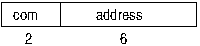
\includegraphics{comm}
    
    The two-bit command is -
    
    \begin{tabular}{ l  l }
        00   & read value, read queue \\
        10   & write static, write queue \\
        01   & read memory \\
        11   & write memory \\
    \end{tabular}
    
    The 6-bit address allows access 64 writable and 64 readable locations
    in the FPGA.
    
    For a write to a static or queue variable the format is -
    
    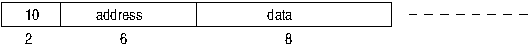
\includegraphics{commw}
    
    where the command is followed by zero or more data bytes (a zero-length
    write has no data but the write can act as a trigger or event).
    There is no response from the FPGA.
    
    For a read from a value or a queue the format is -
    
    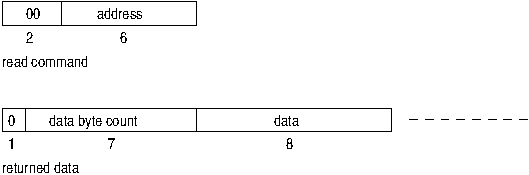
\includegraphics{commr}
    
    where the returned data consists of a data byte count and one or more data
    bytes.
    
    For a write to memory -
    
    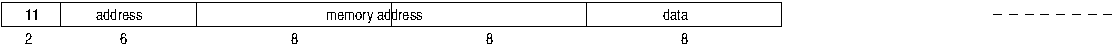
\includegraphics{commmw}
    
    where the command is followed by 16-bit memory address and one or more
    data bytes. There is no response from the FPGA.
    
    For a read from memory -
    
    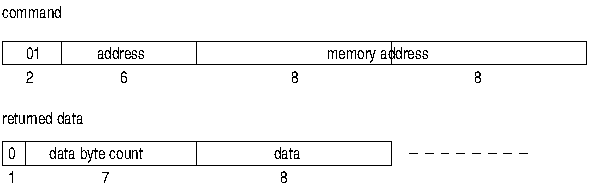
\includegraphics{commmr}
    
    where the command is followed by 16-bit memory address.
    A data byte count and one or more data bytes are returned from the FPGA.

    
    Interrupts are initiated by the FPGA unlike the previous transfers which
    are all initiated by the CPU.
    For an interrupt the FPGA sends a single byte to the CPU. The byte has
    the most significant bit set and the remaining 7 bits indicates the
    interrupt number.

    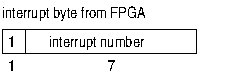
\includegraphics{commint}
    
    An interrupt byte will not be sent during the transmission of a CPU command
    and any associated return data or during a DMA transfer (see below).
    
    DMA requests by the FPGA code are of course carried out by software in
    the CPU (there being no hardware connection for real DMA) and are initiated
    by the FPGA.

    For DMA write from FPGA to CPU -
    
    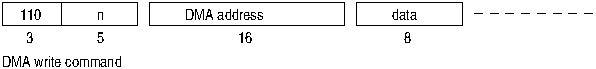
\includegraphics{commdmaw}
    
    For DMA read to FPGA from CPU -
    
    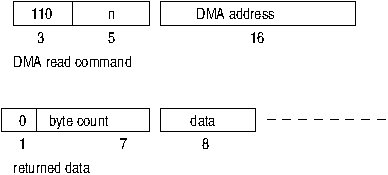
\includegraphics{commdmar}
    

        
    Commands and associated data are written to port file desriptor fd. Data
    received from the FPGA is read from {\bf fd} in the input handler which runs
    in its own thread. A received byte with the top bit set is an interrupt, the
    remaining bits giving the interrupt number (semaphore index). A sem\_post()
    is issued to the semaphore with that index. A received byte with the top bit
    clear is a byte count for data to be received from the FPGA. The following
    bytes indicated by the count are read from {\bf fd} and written to pipe {\bf
    pipefd[1]}. A command expecting received data waits on {\bf pipefd[0]} and
    reads from it (a command knows in advance how many bytes to expect as
    this is contained in the .info file).
    
    
    sem\_wait()
    
    \begin{lstlisting}[gobble=4, language=C]
        #include    "cpu_serial.h"

        #define BSIZE   1024

        sem_t**         sem;
        char**          sem_name;
        char            buffer[BSIZE];
        int             fd;
        struct termios  tio;
        static int      pipefd[2];
        pthread_t       tideh;
        int             ninterrupts;

        int         open_port (char* pname);
        void        close_port ();
        void        write_ (
                        char*   ptr,
                        int     bytes
                    );
        int         read_ (
                        char*   ptr,
                        int     bytes
                    );
        void*       input_handler ();

        void
        open_cpu_serial(char* pname, int interrupts) {
            ninterrupts = interrupts;
            fd = open_port(pname);
            pipe(pipefd);
            if (ninterrupts != 0) {
                sem = (sem_t**)malloc(ninterrupts * sizeof(sem_t*));
                sem_name = (char**)malloc(ninterrupts * sizeof(char*));
                for (int i=0 ; i<ninterrupts ; i++) {
                    sem_name[i] = (char*)malloc(6);
                    sprintf(sem_name[i], "/e%d", i);
                    sem_unlink(sem_name[i]);    // remove if already exists!
                    if ((sem[i] = sem_open(sem_name[i], O_CREAT, 0600, 0)) == SEM_FAILED) {
                        perror("sem_open");
                        exit(1);
                    }
                }
            }
            tideh = thread_start(input_handler, "input_handler", 1);
        }

        void
        close_cpu_serial() {
            pthread_cancel(tideh);
            for (int i=0 ; i<ninterrupts ; i++) {
                sem_close(sem[i]);
                sem_unlink(sem_name[i]);
            }
            close_port();
            close(pipefd[0]);
            close(pipefd[1]);
        }

        void
        comms_write (
            int         mem,        // memory write 1, static or queue write 0
            uint8_t     address,    // FPGA register address
            uint16_t    memaddress, // memory address if required
            int         bytes,      // number of data bytes
            char*       ptr         // pointer to data
        ) {
            char    com = 0x80 | (mem << 6) | address;
            int     i;
            int     n = bytes;

            write_(&com, 1); // send command byte
            if (mem != 0)
                write_((char*)&memaddress, 2); // send memory address
            while (n > 0) {
                i = write(fd, ptr, n);
                n -= i;
                ptr += i;
            }
        }

        void
        write_ (
            char*   ptr,
            int     bytes
        ) {
            int i;

            if (write(fd, ptr, bytes) < 0) {
                fprintf(stderr, "data write error\n");
                exit(1);
            }
        }

        void
        comms_read (
            int         mem,        // memory read 1, value or queue read 0
            uint8_t     address,    // FPGA register address
            uint16_t    memaddress, // memory address if required
            int         bytes,      // number of data bytes to be received
            int         sig,        // 1 if signed, 0 if unsigned
            int         fill,       // number of top bytes to fill
            char*       ptr         // pointer to data destination
        ) {
            char    com = (mem << 6) | address; // set address and memory flag in command
            int     n = bytes;  // byte counter initialisation
            char    snap;       // most significant byte
            char    pad = 0;    // padding byte - 0 or 0xff
            int     i;
            // send command byte
            write_(&com, 1);

            // send memory address if is a memory read
            if (mem != 0)
                write_((char*)&memaddress, 2);

            // receive data and write to destination address
            while (n > 0) {
                i = read_(ptr, n);
                n -= i;
                ptr += i;
            }
            snap = *(ptr - 1);

            // if whole result type has been filled, return
            if (fill == 0)
                return;

            // fill remainder of result with 0x00 (unsigned or +ve) or 0xff (signed and -ve)
            if ((sig != 0) && ((snap & 0x80) != 0))
                pad = 0xff;    // 0xff if signed and -ve
            while (fill-- != 0)
                *ptr++ = pad;   // fill most significant bytes
        }

        int
        read_ (
            char*   ptr,
            int     bytes
        ) {
            int r;
            r = read(pipefd[0], ptr, bytes);
            if (r < 0) {
                fprintf(stderr, "data read error\n");
                exit(1);
            }
            return(r);
        }

        void*
        input_handler () {
            int     r;
            char    c;
            int     n;
            int     bytes;
            char*   ptr;

            for (;;) {
                r = read(fd, &c, 1);
                if (r < 0) {
                    printf("uart read error\n");
                    exit(1);
                }
                n = c & 0x7f;   // byte count or interrupt ID
                if (c & 0x80) {
                    // is an interrupt
                    if (n >= 20)
                        printf("interrupt %d illegal (max 20) - ignored\n", n);
                    else
                        sem_post(sem[n]);
                } else {
                    // is a command return -
                    // read the data
                    bytes = n;
                    ptr = buffer;
                    while (bytes > 0) {
                        r = read(fd, ptr, bytes);
                        bytes -= r;
                        ptr += r;
                    }
                    // write the data back to the command requesting it
                    bytes = n;
                    ptr = buffer;
                    while (bytes > 0) {
                        r = write(pipefd[1], ptr, bytes);
                        bytes -= r;
                        ptr += r;
                    }
                }
            }
        }

        int
        open_port (char* pname) {
            int             fd;
            struct termios  ntio;
            int             flags;

            if (strlen(pname) == 0) {
                fprintf(stderr, "could not find USB serial device");
                exit(1);
            }

            fd = open(pname, O_RDWR | O_NOCTTY | O_NONBLOCK);
            if (fd < 0) {
                fprintf(stderr, "Cannot open USB serial device\n");
                exit(1);
            }
            printf("port %s open\n", pname);

            // Make the file descriptor blocking.
            flags = fcntl(fd, F_GETFL);
            flags &= ~O_NONBLOCK;
            fcntl(fd, F_SETFL, flags);


            tcgetattr(fd, &tio); // get current port settings
            bzero(&ntio,sizeof(ntio)); // clear struct for new port settings
            ntio.c_cflag = CS8 | CREAD | CSTOPB | CLOCAL;
            ntio.c_iflag = IGNPAR;
            ntio.c_oflag = 0;       // OCANON
            ntio.c_lflag = 0;       // ICANON
            ntio.c_cc[VMIN] = 1;    // blocking read until 1 character arrives
            ntio.c_cc[VSTART] = _POSIX_VDISABLE;
            ntio.c_cc[VSTOP] = _POSIX_VDISABLE;
            ntio.c_cc[VINTR] = _POSIX_VDISABLE;
            ntio.c_cc[VQUIT] = _POSIX_VDISABLE;
            ntio.c_cc[VSUSP] = _POSIX_VDISABLE;
            cfsetispeed(&ntio, B115200);
            cfsetospeed(&ntio, B115200);

            tcflush(fd, TCIFLUSH);
            tcsetattr(fd, TCSANOW, &ntio);

            return(fd);
        }

        void
        close_port () {
            // Restore terminal settings
            tcsetattr(fd, TCSANOW, &tio);
            close(fd);
        }

        // Start a thread.
        pthread_t
        thread_start(
            void *  (*func)(void*),
            char *  name,
            int     priority
        ) {
            int                 status;
            struct sched_param  sp;
            pthread_t           tid;

            if ((status = pthread_create(&tid, NULL, func, NULL)) != 0) {
	        printf("thread_start(): pthread_create() failed thread '%s' (err = %s)\n",
	            name, strerror(status));
                exit(1);
            }

            sp.sched_priority = priority;

            status = pthread_setschedparam(tid, SCHED_RR, &sp);
            if (status != 0) {
    	        printf("thread_start(): pthread_setschedparam() failed for thread '%s' (err = %s)\n",
	            name, strerror(status));
                exit(1);
            }
            return(tid);
        }
    \end{lstlisting}
    


\chapter{cpu\_serial.py}

    The Python3 version of this code functions the same way as the
    C version above -

    \begin{lstlisting}[gobble=4, language=Python]
        import os
        import fcntl
        import termios
        import queue
        import threading

        tio = None
        infile = None
        fd = None
        q = queue.Queue()

        # Write data to FPGA.
        #   mem         0 if static or queue write, 1 if memory write
        #   address     FPGA interface address
        #   memaddress  memory address if mem == 1
        #   dba         byte array of data to send
        #
        def comms_write (mem, address, memaddress, dba):
            ba = bytearray()
            ba += bytes([0x80 | (mem << 6) | address])          # command
            if mem != 0:
                ba += memaddress.to_bytes(2, byteorder='little')# append memory address
            if dba != None:
                ba += dba                                       # append data
            os.write(fd, ba)                                    # write to FPGA

        # Read data from FPGA.
        #   mem         0 if value or queue read, 1 if memory read
        #   address     FPGA interface address
        #   memaddress  memory address if mem == 1
        #   bytes       data length - NOT USED HERE (required by Zynq)!
        #
        def comms_read (mem, address, memaddress, bytecount):
            global q
            wba = bytearray()
            wba += bytes([(mem << 6) | address])                # command - address and memory flag
            if mem != 0:
                wba += memaddress.to_bytes(2, byteorder='little')# append memory address
            os.write(fd, wba)                                   # write to FPGA
            return(q.get())                                     # read response from FPGA


        # Close the serial port to the FPGA.
        def close_port ():
            # Restore terminal settings
            tcsetattr(fd, TCSANOW, tio)
            close(fd)

        # Handle input from FPGA via serial port.
        def input_handler ():
            global fd
            global q
            while True:
                try:
                    r = os.read(fd, 1)
                except OSError:
                    print("UART read error")
                    exit(1)
                c = r[0]
                n = c & 0x7f    # Note: max of 127 bytes
                if c & 0x80:
                    # is an interrupt
                    if n >= 20:
                        print("interrupt " + str(n) + " illegal (max 19)")
                        exit(1)
                    else:
                        semaphores[n].release()
                else:
                    # is a command return - read the data            
                    buff = bytearray()
                    while n > 0:
                        buff += bytes(os.read(fd, n))
                        n -= len(buff)
                    q.put(buff)

        # Open the serial port to the FPGA.
        def open_cpu_serial (pname, ninterrupts):
            global fd
            global tio
            global semaphores

            if len(pname) == 0:
                print("could not find USB serial device" + pname)
                exit(1)
            try:
                # Open initially as non-blocking so it does not wait trying to read
                # as it is opened.
                fd = os.open(pname, os.O_RDWR | os.O_NOCTTY | os.O_NONBLOCK)
            except OSError:
                print("Cannot open USB serial device")
                exit(1)

            # Having opened the file and continued, now make the file
            # descriptor blocking.
            flags = fcntl.fcntl(fd, fcntl.F_GETFL)
            flags &= ~os.O_NONBLOCK
            fcntl.fcntl(fd, fcntl.F_SETFL, flags)

            tio = termios.tcgetattr(fd) # get current port settings
            ntio = termios.tcgetattr(fd)

            ntio[0] = termios.IGNPAR                # iflags
            ntio[1] = 0                             # oflags - OCANON
            ntio[2] = termios.CS8 | termios.CREAD | termios.CSTOPB | termios.CLOCAL # cflags
            ntio[3] = 0                             # lflags - ICANON
            ntio[4] = termios.B115200               # ispeed
            ntio[5] = termios.B115200               # ospeed
            ntio[6][termios.VMIN] = 1               # blocking read until 1 character arrives
            ntio[6][termios.VSTART] = 0
            ntio[6][termios.VSTOP] = 0
            ntio[6][termios.VINTR] = 0
            ntio[6][termios.VQUIT] = 0
            ntio[6][termios.VSUSP] = 0

            termios.tcflush(fd, termios.TCIFLUSH)
            termios.tcsetattr(fd, termios.TCSANOW, ntio)

            # Create and start the input handler thread.
            t = threading.Thread(target=input_handler, args=())
            t.start()

            global semaphores
            semaphores = []
            for i in range(ninterrupts):
                semaphores.append(threading.Semaphore(0))

        def close_cpu_serial ():
            close_port()


        def open_port (pname):
            if pname == "":
                print("Cannot find USB serial device " + pname)
                exit(1)
            fd = open(pname, 'r')

        def close_port ():
            # Restore terminal settings
            termios.tcsetattr(fd, termios.TCSANOW, tio)
            #os.close(fd) HANGS WAITING ON THREAD!
    \end{lstlisting}




\input{Zynq_device_tree}

\input{licence}



\chapter{Alphabetic List of all Inbuilt and Library Modules, Procedures and
Functions}

    \pagebreak

Abbreviations - \\
I M - inbuilt module \\
I P - inbuilt procedure \\
I F - inbuilt function \\
L M - library module \\
L P - library procedure \\
L F - library function \\
L C - library class \\
L CM - library class module\\
L CP - library class procedure\\
L CF - library class function\\



\pagebreak

\begin{tabular}{l l l l}
\hyperref[sec:ifabs]{abs} & I F & absolute value function & \refp{sec:ifabs} \\
\hyperref[sec:ifaccept]{accept} & I F & ignore clock domain differences & \refp{sec:ifaccept} \\
\hyperref[sec:ifacos]{acos} & I F & trigonometric arc cosine function & \refp{sec:ifacos} \\
\hyperref[sec:ipaddmodeatt]{addmodeattribute} & I P & add attribute to the mode attribute map & \refp{sec:ipaddmodeatt} \\
\hyperref[sec:lpaddncfline]{addncfline} & L P & add line to NCF file & \refp{sec:lpaddncfline} \\
\hyperref[sec:ifaddsub]{addsub} & I F & conditionally add or subtract & \refp{sec:ifaddsub} \\
\hyperref[sec:lpaddxdcline]{addxdcline} & L P & add line to XDC file & \refp{sec:lpaddxdcline} \\
\hyperref[sec:ipappend]{append} & I P & append a list entry & \refp{sec:ipappend} \\
\hyperref[sec:ipappendall]{appendall} & I P & append entries from another list & \refp{sec:ipappendall} \\
\hyperref[sec:lpappncf]{append\_ncf\_file} & L P & append a file to the NCF file & \refp{sec:lpappncf} \\
\hyperref[sec:ipargadjust]{argadjust} & I P & adjust arguments for arithmetic operations & \refp{sec:ipargadjust} \\
\hyperref[sec:ifarglist]{arglist} & I F & pass lists, arrays or maps of arguments & \refp{sec:ifarglist} \\
\hyperref[sec:lfargstomap]{argstomap} & L F & create a map from key=value arguments & \refp{sec:lfargstomap} \\
\hyperref[sec:lmarraytoqueue]{array\_to\_queue} & L M & serialise an array to a queue & \refp{sec:lmarraytoqueue} \\
\hyperref[sec:ifarraytostr]{arraytostr} & I F & convert an integer array to a string & \refp{sec:ifarraytostr} \\
\hyperref[sec:ifarraytype]{arraytype} & I F & array type of a variable or expression & \refp{sec:ifarraytype} \\
\hyperref[sec:ifasin]{asin} & I F & trigonometric arc sine function & \refp{sec:ifasin} \\
\hyperref[sec:ipassert]{assert} & I P & assert a value mode variable for a clock cycle & \refp{sec:ipassert} \\
\hyperref[sec:lpassign]{assign} & L P & generalised assignment & \refp{sec:lpassign} \\
\hyperref[sec:lfasyncqueuespaces]{asyncqueuespaces} & L F & space count for asynchronous queue & \refp{sec:lfasyncqueuespaces} \\
\hyperref[sec:lfasyncqueuewords]{asyncqueuewords} & L F & word count for asynchronous queue & \refp{sec:lfasyncqueuewords} \\
\hyperref[sec:ifatan]{atan} & I F & single argument trigonometric arc tangent function & \refp{sec:ifatan} \\
\hyperref[sec:ifatan2]{atan2} & I F & two argument trigonometric arc tangent function & \refp{sec:ifatan2} \\
\hyperref[sec:ifattribute]{attribute} & I F & get an attribute from a variable & \refp{sec:ifattribute} \\
\hyperref[sec:ipattributeproc]{attributeprocedure} & I P & register a procedure to handle attributes & \refp{sec:ipattributeproc} \\
\hyperref[sec:ifattributes]{attributes} & I F & get the attributes of a variable & \refp{sec:ifattributes} \\
\hyperref[sec:ipattributes]{attributes} & I P & assign attributes to a variable & \refp{sec:ipattributes} \\
\hyperref[sec:ifbiasedexponent]{biasedexponent} & I F & target float biased exponent & \refp{sec:ifbiasedexponent} \\
\hyperref[sec:ifbiasedexponentwidth]{biasedexponentwidth} & I F & width of target float biased exponent & \refp{sec:ifbiasedexponentwidth} \\
\hyperref[sec:lfbintogray]{bin\_to\_gray} & L F & convert binary count to gray count & \refp{sec:lfbintogray} \\
\hyperref[sec:lfbitset]{bitset} & L F & test if a bit is set & \refp{sec:lfbitset} \\
\hyperref[sec:ifbitsfor]{bitsfor} & I F & number of bits to represent an integer - DEPRECATED! & \refp{sec:ifbitsfor} \\
%    \hyperref[sec:lfbram2]{bram2} & L F & create extended dual-port registered output memory & \refp{sec:lfbram2} \\
\hyperref[sec:lmcapture]{capture} & L M & capture a data sequence & \refp{sec:lmcapture} \\
\hyperref[sec:ifcast]{cast} & I F & cast a value to a new type or type width & \refp{sec:ifcast} \\
\hyperref[sec:lfcdatas]{cdatas} & L F & generate C name array for 3PL enum type & \refp{sec:lfcdatas} \\
\hyperref[sec:ifceil]{ceil} & I F & round float to nearest integer towards $+\infty$ & \refp{sec:ifceil} \\
\hyperref[sec:ipchange]{change} & I P & change a list entry & \refp{sec:ipchange} \\
\hyperref[sec:lpcinclude]{cinclude} & L P & convert a C include file & \refp{sec:lpcinclude} \\
\hyperref[sec:ipclass]{class} & I P & create a variable of type "class" & \refp{sec:ipclass} \\
\hyperref[sec:lpclkdcm]{clkdcm} & L P & create a DCM digital clock manager & \refp{sec:lpclkdcm} \\
\hyperref[sec:lpclkdlle]{clkdlle} & L P & create an extended Spartan2, Virtex or VirtexE DLL& \refp{sec:lpclkdlle} \\
\hyperref[sec:lpclkdllhf]{clkdllhf} & L P & create a high frequency Spartan2, Virtex or VirtexE DLL& \refp{sec:lpclkdllhf} \\
\hyperref[sec:lpclkdll]{clkdll} & L P & create a DLL delay-locked loop clock manager & \refp{sec:lpclkdll} \\
\hyperref[sec:lpmmcma]{clkmmcm\_adv} & L P & create an advanced MMCM multi-mode clock manager & \refp{sec:lpmmcma} \\
\hyperref[sec:lpmmcmb]{clkmmcm\_base} & L P & create a basic MMCM multi-mode clock manager & \refp{sec:lpmmcmb} \\
\hyperref[sec:ipclock]{clock} & I P & create one or more clock variable & \refp{sec:ipclock}   \\
\hyperref[sec:lfclockused]{clockused} & L F & determine if a clock variable has been used & \refp{sec:lfclockused}   \\
\hyperref[sec:lpclockbufg]{clockbufg} & L P & a BUFG clock buffer & \refp{sec:lpclockbufg} \\
\hyperref[sec:lpclockbufio]{clockbufio} & L P & a local clock buffer & \refp{sec:lpclockbufio} \\
\hyperref[sec:ipclockfromexpr]{clockfromexpr} & I P & drive a clock from an expression & \refp{sec:ipclockfromexpr} \\
\hyperref[sec:lpclockmuxbuffer]{clockmuxbuffer} & L P & a clock mux/buffer & \refp{sec:lpclockmuxbuffer} \\
\hyperref[sec:lpclockmuxbufferdis]{clockmuxbufferdisable} & L P & a clock mux/buffer with disable & \refp{sec:lpclockmuxbufferdis} \\
\hyperref[sec:lfclockparams]{clock\_params} & L P & derive clock synthesis parameters & \refp{sec:lpclockparams} \\
\hyperref[sec:lfclockparams]{clock\_params} & L F & derive clock synthesis parameters & \refp{sec:lfclockparams} \\
\hyperref[sec:ipclose]{close} & I P &close a file & \refp{sec:ipclose} \\
\hyperref[sec:ipcmemory]{cmemory} & I P & create a combinatorial output memory & \refp{sec:ipcmemory}   \\ 
\hyperref[sec:ifcmemoryread]{cmemoryread} & I F & read a combinatorial output memory & \refp{sec:ifcmemoryread} \\
\hyperref[sec:ipcmemorywrite]{cmemorywrite} & I P & write to a combinatorial output memory & \refp{sec:ipcmemorywrite} \\     
%\hyperref[sec:ifcomponentpointer]{componentpointer} & I F & get a pointer to a static variable component & \refp{sec:ifcomponentpointer} \\
%\hyperref[sec:ipconnect]{connect} & I P & connect two signals & \refp{sec:ipconnect} \\
\end{tabular}

\pagebreak

\begin{tabular}{l l l l}
%\hyperref[sec:ifcomponenttype]{componenttype} & I F & get the type of a variable component & \refp{sec:ifcomponenttype} \\
\hyperref[sec:ifcopy]{copy} & I F & copy a list or map & \refp{sec:ifcopy} \\
\hyperref[sec:ifcosin]{cos} & I F & trigonometric cosine function & \refp{sec:ifcosin} \\

\hyperref[chap:lmxilcpulib]{cpu\_api} & L C & a CPU/FPGA interface class (UART, ZYNQ) & \refp{chap:lmxilcpulib} \\
\hyperref[sec:lmzynqrddma]{cpu\_api.dma\_read} & L CM & DMA transfer from memory to FPGA (ZYNQ) & \refp{sec:lmzynqrddma} \\
\hyperref[sec:lmzynqwrdma]{cpu\_api.dma\_write} & L CM & DMA transfer from FPGA to memory (ZYNQ) & \refp{sec:lmzynqwrdma} \\
\hyperref[sec:lpcpurd]{cpu\_api.read} & L CP & a CPU-readable interface (UART, ZYNQ) & \refp{sec:lpcpurd} \\
\hyperref[sec:lpcpurdmem]{cpu\_api.read\_memory} & L CP & a CPU-readable interface to a memory (UART, ZYNQ) & \refp{sec:lpcpurdmem} \\
\hyperref[sec:lpcpurdqueue]{cpu\_api.read\_queue} & L CP & CPU read from a queue variable (UART, ZYNQ) & \refp{sec:lpcpurdqueue} \\
\hyperref[sec:lpcpurdvalue]{cpu\_api.read\_value} & L CP & CPU read from a value (UART, ZYNQ) & \refp{sec:lpcpurdvalue} \\
\hyperref[sec:lprcvevent]{cpu\_api.receive\_event} & L CP & interrupt the CPU (UART, ZYNQ) & \refp{sec:lprcvevent} \\
\hyperref[sec:lpcpuwr]{cpu\_api.write} & L CP & a CPU-writable interface (UART, ZYNQ) & \refp{sec:lpcpuwr} \\
\hyperref[sec:lmzynqdmabufr]{cpu\_api.write\_dma\_buffer} & L CM & DMA transfer to CPU RAM (ZYNQ) & \refp{sec:lmzynqdmabufr} \\
\hyperref[sec:lpcpuwrmem]{cpu\_api.write\_memory} & L CP & a CPU-writable interface to a memory (UART, ZYNQ) & \refp{sec:lpcpuwrmem} \\
\hyperref[sec:lpcpuwrqueue]{cpu\_api.write\_queue} & L CP & a CPU write to a queue variable (UART, ZYNQ) & \refp{sec:lpcpuwrqueue} \\
\hyperref[sec:lpinterrupt]{cpu\_api.api.interrupt} & L CP & interrupt the CPU (UART, ZYNQ) & \refp{sec:lpinterrupt} \\

\hyperref[sec:lmcrc32]{crc32} & L M & Virtex5 and later 32 bit CRC & \refp{sec:lmcrc32} \\
\hyperref[sec:lmcrc64]{crc64} & L M & Virtex5 and later 64 bit CRC & \refp{sec:lmcrc64} \\
\hyperref[sec:lmcrc816]{crc\_8\_16} & L M & 16 bit CRC from 8 bit data & \refp{sec:lmcrc816} \\
\hyperref[sec:lmcrc1616]{crc\_16\_16} & L M & 16 bit CRC from 16 bit data & \refp{sec:lmcrc1616} \\
\hyperref[sec:lmcrcblock]{crcblock} & L M & block 32 bit data with a CRC & \refp{sec:lmcrcblock} \\
\hyperref[sec:lmcrcunblock]{crcunblock} & L M & unblock 32 bit data with a CRC & \refp{sec:lmcrcunblock} \\
\hyperref[sec:lmcread]{cread} & L M & read combinatorial output memory to a queue & \refp{sec:lmcread} \\
\hyperref[sec:ifcspan]{cspan} & I F & head string selected by characters not in a set & \refp{sec:ifcspan} \\
\hyperref[sec:lfctypes]{ctypes} & L F & converts 3PL types to C types & \refp{sec:lfctypes} \\
\hyperref[sec:ifcurrentclock]{currentclock} & I F & get the current clock variable & \refp{sec:ifcurrentclock} \\
\hyperref[sec:ifcurrentelement]{currentelement} & I F & get the current element identifier & \refp{sec:ifcurrentelement} \\
\hyperref[sec:lmcwrite]{cwrite} & L M & write combinatorial output memory from queue & \refp{sec:lmcwrite} \\
\hyperref[sec:lmdcireset]{dcireset} & L M & reset DCI pins & \refp{sec:lmdcireset} \\
\hyperref[sec:lfdeglitch]{deglitch} & L F & deglitch an input signal & \refp{sec:lfdeglitch} \\
\hyperref[sec:ifdeflate]{deflate} & I F & compress a string & \refp{sec:ifdeflate} \\
\hyperref[sec:lfdelay]{delay} & L F & fixed delay & \refp{sec:lfdelay} \\
\hyperref[sec:imdel]{del} & I M & variable length delay line & \refp{sec:imdel} \\
\hyperref[sec:lfdel]{del} & L F & variable length delay line & \refp{sec:lfdel} \\
\hyperref[sec:lmdemultiplex]{demultiplex} & L M & demultiplex a source & \refp{sec:lmdemultiplex} \\
\hyperref[sec:lmdemultiplex]{demultiplex\_e} & L M & demultiplex a source using port number & \refp{sec:lmdemultiplex} \\
\hyperref[sec:lmdemultiplex]{demultiplex\_l} & L M & demultiplex a source using port bit & \refp{sec:lmdemultiplex} \\
\hyperref[sec:ipdesignname]{designname} & I P & change the design name & \refp{sec:ipdesignname} \\
\hyperref[sec:ifdimension]{dimension} & I F & dimension - get a dimension of an array or size of a map or list & \refp{sec:ifdimension} \\
\hyperref[sec:ifdimensions]{dimensions} & I F & get the number of dimensions of an array & \refp{sec:ifdimensions} \\
\hyperref[sec:ipdirective]{directive} & I P & enter a directive & \refp{sec:ipdirective} \\
\hyperref[sec:ifdirective]{directive} & I F & get the value of a directive & \refp{sec:ifdirective} \\
\hyperref[sec:ifdirectives]{directives} & I F & get the global directives map & \refp{sec:ifdirectives} \\
\hyperref[sec:ifdirexists]{direxists} & I F & determine if a directive exists & \refp{sec:ifdirexists} \\
\hyperref[sec:lmdivide]{divide} & L M & pipelined integer division-remainder & \refp{sec:lmdivide} \\
\hyperref[sec:ipdivrem]{divrem} & I P & combined quotient and remainder & \refp{sec:ipdivrem} \\
\hyperref[sec:ifdomain]{domain} & I F & get the clock domain for a variable & \refp{sec:ifdomain} \\
\hyperref[sec:lpdsp48]{dsp48} & L P & create a DSP48 block for Virtex4 FPGAs & \refp{sec:lpdsp48} \\
\hyperref[sec:lpdsp48a]{dsp48a} & L P & create a DSP48 block for Spartan6 FPGAs & \refp{sec:lpdsp48a} \\
\hyperref[sec:lpdsp48e]{dsp48e} & L P & create a DSP48E block for Virtex5 FPGAs & \refp{sec:lpdsp48e} \\
\hyperref[sec:lpdsp48e1]{dsp48e1} & L P & create a DSP48E1 block for Virtex6 FPGAs & \refp{sec:lpdsp48e1} \\
\hyperref[sec:lmdspaddsub]{dspaddsub} & L M & DSP add/subtract & \refp{sec:lmdspaddsub} \\
\hyperref[sec:lmdspcounter]{dspcounter} & L M & DSP counter & \refp{sec:lmdspcounter} \\
\hyperref[sec:lmdsplog]{dsplog} & L M & DSP logical operation & \refp{sec:lmdsplog} \\
\hyperref[sec:lmdspmul]{dspmul} & L M & DSP multiply & \refp{sec:lmdspmul} \\
\hyperref[sec:lmdspmuladd]{dspmuladd} & L M & DSP multiply and add & \refp{sec:lmdspmuladd} \\
\hyperref[sec:lmdspmulsub]{dspmulsub} & L M & DSP multiply and subtract & \refp{sec:lmdspmulsub} \\
\hyperref[sec:lmdspsubmul]{dspsubmul} & L M & DSP subtract and multiply & \refp{sec:lmdspsubmul} \\
\hyperref[sec:ifdutycycle]{dutycycle} & I F & get the duty cycle of a clock variable & \refp{sec:ifdutycycle} \\
\end{tabular}

\pagebreak

\begin{tabular}{l l l l}
\hyperref[sec:ifelapsedtime]{elapsedtime} & I F & get the elapsed time & \refp{sec:ifelapsedtime} \\
\hyperref[sec:ipelement]{element} & I P & add an element to the EDIF netlist & \refp{sec:ipelement} \\
\hyperref[sec:lpelementaddncf]{elementaddncf} & L P & add constraint to NCF file for an element & \refp{sec:lpelementaddncf} \\
\hyperref[sec:lpelementBinProperty]{elementBinProperty} & L P & add a property of type "int" to an element in binary format & \refp{sec:lpelementBinProperty} \\
\hyperref[sec:lpelementcheck]{elementcheck} & I P & check that a Xilinx element is allowed in the current device family & \refp{sec:lpelementcheck} \\
\hyperref[sec:lfelementcheck]{elementcheck} & I F & check that a Xilinx element is allowed in the current device family & \refp{sec:lfelementcheck} \\
\hyperref[sec:ipelmntinclk]{elementclockinput} & I P & connect a clock input signal to an EDIF netlist element & \refp{sec:ipelmntinclk} \\
\hyperref[sec:ipelementend]{elementend} & I P & complete construction of an EDIF netlist element & \refp{sec:ipelementend} \\
\hyperref[sec:lpelementFloatProperty]{elementFloatProperty} & L P & add a property of type "float" to an element & \refp{sec:lpelementFloatProperty} \\
\hyperref[sec:lpelementHexProperty]{elementHexProperty} & L P & add a property of type "int" to an element in hexadecimal format & \refp{sec:lpelementHexProperty} \\
\hyperref[sec:ipelmntin]{elementinput} & I P & connect an input signal to an EDIF netlist element & \refp{sec:ipelmntin} \\
\hyperref[sec:lpelementIntProperty]{elementIntProperty} & L P & add a property of type "int" to an element & \refp{sec:lpelementIntProperty} \\
\hyperref[sec:lpelementLogProperty]{elementLogProperty} & L P & add a property of type "log" to an element & \refp{sec:lpelementLogProperty} \\
\hyperref[sec:ipelmntout]{elementoutput} & I P & connect an output signal to an EDIF netlist element & \refp{sec:ipelmntout} \\
\hyperref[sec:ipelementproperty]{elementproperty} & I P & set an element property & \refp{sec:ipelementproperty} \\
\hyperref[sec:lpelementStrProperty]{elementStrProperty} & L P & add a property of type "str" to an element & \refp{sec:lpelementStrProperty} \\
\hyperref[sec:ipelmntoutts]{elementtsoutput} & I P & connect a 3-state output signal to an EDIF netlist element & \refp{sec:ipelmntoutts} \\
\hyperref[sec:ipemptyvalue]{emptyvalue} & I P & clear a value-mode variable & \refp{sec:ipemptyvalue} \\
\hyperref[sec:ifendswith]{endswith} & I F & a string is the tail of another & \refp{sec:ifendswith} \\
\hyperref[sec:ifentries]{entries} & I F & get the number of entries in a list or map - DEPRECATED & \refp{sec:ifentries} \\
\hyperref[sec:ipenum]{enum} & I P & create an enumerated type & \refp{sec:ipenum} \\
\hyperref[sec:ipenumv]{enumv} & I P & create an enumerated type & \refp{sec:ipenumv} \\
\hyperref[sec:ifenv]{env} & I F & get the environment variables & \refp{sec:ifenv} \\
\hyperref[sec:ipexec]{exec} & I P & execute a command & \refp{sec:ipexec} \\
\hyperref[sec:ifexists]{exists} & I F & determine if an identifier is recognised - DEPRECATED! & \refp{sec:ifexists} \\
\hyperref[sec:ipexit]{exit} & I P & terminate execution & \refp{sec:ipexit} \\
\hyperref[sec:ifexp]{exp} & I F & e to a power & \refp{sec:ifexp} \\
\hyperref[sec:iffamily]{family} & I F & string identifying platform & \refp{sec:iffamily} \\
\hyperref[sec:ipexport]{export} & I P & export a 'core' & \refp{sec:ipexport} \\
\hyperref[sec:ipexternal]{external} & I P & declare a signal as an EDIF port & \refp{sec:ipexternal} \\
\hyperref[sec:lmfadd]{fadd} & L M & floating add & \refp{sec:lmfadd} \\
\hyperref[sec:lmfdiv]{fdiv} & L M & floating divide & \refp{sec:lmfdiv} \\
\hyperref[sec:lpfdre]{fdre} & L P & Create an FDRE flip-flop & \refp{sec:lpfdre} \\
\hyperref[sec:lpfdre]{fdrse} & L P & Create an FDRSE flip-flop & \refp{sec:lpfdrse} \\
\hyperref[sec:lpfdse]{fdse} & L P & Create an FDSE flip-flop & \refp{sec:lpfdse} \\
\hyperref[sec:lpfdce]{fdce} & L P & Create an FDCE flip-flop & \refp{sec:lpfdce} \\
\hyperref[sec:lpfdpe]{fdpe} & L P & Create an FDPE flip-flop & \refp{sec:lpfdpe} \\
\hyperref[sec:lmfifo]{fifo} & L M & a fifo with static interface & \refp{sec:lmfifo} \\
\hyperref[sec:ipfile]{file} & I P & create file variables & \refp{sec:ipfile} \\
\hyperref[sec:iffilecanread]{filecanread} & I F & check if a file is readable & \refp{sec:iffilecanread} \\
\hyperref[sec:iffilecanwrite]{filecanwrite} & I F & check if a file is writable & \refp{sec:iffilecanwrite} \\
\hyperref[sec:iffiledelete]{filedelete} & I F & delete a file & \refp{sec:iffiledelete} \\
\hyperref[sec:iffileexists]{fileexists} & I F & check if a file exists & \refp{sec:iffileexists} \\
\hyperref[sec:iffilegetparent]{filegetparent} & I F & get the path to the file & \refp{sec:iffilegetparent} \\
\hyperref[sec:iffileisdir]{fileisdir} & I F & check if a file is a directory & \refp{sec:iffileisdir} \\
\hyperref[sec:iffileisfile]{fileisfile} & I F & check if a file is a file & \refp{sec:iffileisfile} \\
\hyperref[sec:iffilelastmod]{filelastmod} & I F & get the time of last modification & \refp{sec:iffilelastmod} \\
\hyperref[sec:iffilelength]{filelength} & I F & get the file length in bytes & \refp{sec:iffilelength} \\
\hyperref[sec:iffilelist]{filelist} & I F & get a list of files and directories & \refp{sec:iffilelist} \\
\hyperref[sec:iffilelistdirs]{filelistdirs} & I F & get a list of directories & \refp{sec:iffilelistdirs} \\
\hyperref[sec:iffilelistfiles]{filelistfiles} & I F & get a list of files & \refp{sec:iffilelistfiles} \\
\hyperref[sec:iffilemkdir]{filemkdir} & I F & create a directory & \refp{sec:iffilemkdir} \\
\hyperref[sec:iffilerename]{filerename} & I F & rename a file or directory & \refp{sec:iffilerename} \\
\hyperref[sec:iffilesetreadonly]{filesetreadonly} & I F & set a file or directory read-only & \refp{sec:iffilesetreadonly} \\
\hyperref[sec:iffind]{find} & I F & find a substring using a regular expression & \refp{sec:iffind} \\
%\hyperref[sec:iffirst]{first} & I F & get the first value of an enum & \refp{sec:iffirst} \\
\hyperref[sec:ipfloat]{float} & I P & create immediate floating point variables & \refp{sec:ipfloat} \\
\hyperref[sec:iffloatisnegative]{floatisnegative} & I F & sign of target float & \refp{sec:iffloatisnegative} \\
\hyperref[sec:iffloor]{floor} & I F & round float to nearest integer towards $-\infty$ & \refp{sec:iffloor} \\
\end{tabular} 

\pagebreak

\begin{tabular}{l l l l}
\hyperref[sec:lmfmul]{fmul} & L M & floating multiply & \refp{sec:lmfmul} \\
\hyperref[sec:lmfneg]{fneg} & L M & negate a floating point value & \refp{sec:lmfneg} \\
\hyperref[sec:ifformat]{format} & I F & format values into a string & \refp{sec:ifformat} \\
\hyperref[sec:lfforcecast]{forcecast} & L F & force a prohibited cast & \refp{sec:lfforcecast} \\
\hyperref[sec:ipfprintf]{fprintf} & I P & print a formatted line to an output file & \refp{sec:ipfprintf} \\
\hyperref[sec:iffrequency]{frequency} & I F & get the frequency of a clock variable & \refp{sec:iffrequency} \\
\hyperref[sec:ipfscanf]{fscanf} & I P & scan a line from a file into variables & \refp{sec:ipfscanf} \\
\hyperref[sec:lmfsub]{fsub} & L M & floating subtract & \refp{sec:lmfsub} \\
\hyperref[sec:lpgenerateconstraints]{generateConstraints} & I F & generate constraint file entries from I/O mode variable attributes & \refp{sec:lpgenerateconstraints} \\
\hyperref[sec:ifget]{get} & I F & get a list or map entry & \refp{sec:ifget} \\
\hyperref[sec:lfgetbit]{getbit} & L F & get a bit & \refp{sec:lfgetbit} \\
%\hyperref[sec:ifgetfield]{getfield} & I F & get the nth field from a struct & \refp{sec:ifgetfield} \\
\hyperref[sec:lfgetiostandard]{getiostandard} & L F & get the I/O standard for a pin or pins & \refp{sec:lfgetiostandard} \\
\hyperref[sec:lmgtcustom16]{gt\_custom\_16}& L M & a 16-bit Rocket high-speed serial I/O channel & \refp{sec:lmgtcustom16} \\
\hyperref[sec:lpgtpdual]{gtp\_dual}& L M & create a GTP dual high-speed serial I/O channel tile & \refp{sec:lpgtpdual} \\
\hyperref[sec:lmgtpdual16]{gtp\_dual\_16}& L M & a 16-bit dual high-speed serial I/O channel tile & \refp{sec:lmgtpdual16} \\
\hyperref[sec:ifhadeof]{hadeof} & I F & had EOF on the last file read & \refp{sec:ifhadeof} \\
%\hyperref[sec:ifhasfield]{hasfield} & I F & check if a struct has a specific field & \refp{sec:ifhasfield} \\
\hyperref[sec:ifhasnext]{hasnext} & I F & is there a next value of an enum & \refp{sec:ifhasnext} \\
\hyperref[sec:ifhasqueuereads]{hasqueuereads} & I F & does an argument contain queue reads & \refp{sec:ifhasqueuereads} \\
\hyperref[sec:ifhasprev]{hasprev} & I F & is there a previous value of an enum & \refp{sec:ifhasprev} \\
\hyperref[sec:ifhead]{head} & I F & get the head of a string & \refp{sec:ifhead} \\
\hyperref[sec:lpiddr]{iddr} & L P & input double data rate interface & \refp{sec:lpiddr} \\
\hyperref[sec:lpidelay]{idelay} & L P & input data delay & \refp{sec:lpidelay} \\
\hyperref[sec:ipident]{ident} & L P &  extract an identifier from an argument & \refp{sec:ipident} \\
\hyperref[sec:ifidentifier]{identifier} & I F & get the identifier of a variable & \refp{sec:ifidentifier} \\
\hyperref[sec:ipimport]{import} & I P & import a 'core' & \refp{sec:ipimport} \\
%\hyperref[sec:ifimtotargtype]{imtotargtype} & I F & convert an immediate type to a target type & \refp{sec:ifimtotargtype} \\
%\hyperref[sec:ipincludedir]{includedir} & I P & add directory for include path & \refp{sec:ipincludedir} \\
\hyperref[sec:ifincldirs]{includedir} & I F & get the directories searched for module and source files & \refp{sec:ifincldirs} \\
\hyperref[sec:lfincrdecr]{incrdecr} & L F & dynamically increment or decrement & \refp{sec:lfincrdecr} \\
\hyperref[sec:ipinput]{input} & I P & create an input mode variable & \refp{sec:ipinput} \\
\hyperref[sec:ipint]{int} & I P &  create one or more immediate integer variables & \refp{sec:ipint} \\
\hyperref[sec:ifinttobinstring]{inttobinstring} & I F & get a binary string representing an integer & \refp{sec:ifinttobinstring} \\
\hyperref[sec:ifinttohexstring]{inttohexstring} & I F & get a hex string representing an integer & \refp{sec:ifinttohexstring} \\
\hyperref[sec:lpioconstraint]{IOconstraint} & L P & add an I/O constraint to the constraints file & \refp{sec:lpioconstraint} \\
\hyperref[sec:lpiodelay]{iodelay} & L P & input/output data delay & \refp{sec:lpiodelay} \\
\hyperref[sec:lpiopins]{iopins} & L P & create FPGA pin specifications & \refp{sec:lpiopins} \\
\hyperref[sec:lfisclear]{isclear} & L F & verify a run of clear bits & \refp{sec:lfisclear} \\
\hyperref[sec:lpiserdes]{iserdes} & L P & input deserialiser & \refp{sec:lpiserdes} \\
\hyperref[sec:ifisnull]{isnull} & I F & determine if null & \refp{sec:ifisnull}   \\
\hyperref[sec:ifisread]{isread} & I F & determine when a queue variable is read & \refp{sec:ifisread} \\
\hyperref[sec:ifissigned]{issigned} & I F & determine if a type is signed & \refp{sec:ifissigned}   \\
\hyperref[sec:lfisset]{isset} & L F & verify a run of set bits & \refp{sec:lfisset} \\
\hyperref[sec:ifiswritten]{iswritten} & I F & determine when a static or queue variable is written & \refp{sec:ifiswritten} \\
\hyperref[sec:ifisstruct]{isstruct} & I F & determine if a variable type is a struct & \refp{sec:ifisstruct} \\
\hyperref[sec:ifistargconst]{istargconst} & I F & check if a value mode variable is a constant & \refp{sec:ifistargconst}   \\
\hyperref[sec:lmitof]{itof} & L M & convert an integer to a floating point value & \refp{sec:lmitof} \\
\hyperref[sec:lfjsontype]{jsontype} & L F & generate a JSON string from a 3PL type & \refp{sec:lfjsontype} \\
%\hyperref[sec:iflast]{last} & I F & get the last value of an enum & \refp{sec:iflast} \\
\hyperref[sec:lfsr]{lfsr} & L F & linear feedback shift register & \refp{sec:lfsr} \\
\hyperref[sec:iflistattrs]{listattributes} & I F & get a list of variable attributes & \refp{sec:iflistattrs} \\
\hyperref[sec:ipliststt]{liststacks} & I P & list the current state of the body and scope stacks & \refp{sec:ipliststt} \\
\hyperref[sec:iflistvars]{listvars} & I F & get a list of variables & \refp{sec:iflistvars} \\
\hyperref[sec:iflocation]{location} & I F & get the current source location & \refp{sec:iflocation} \\
\hyperref[sec:iplog]{log} & I P & create one or more immediate logical variables & \refp{sec:iplog} \\
\hyperref[sec:iflog]{log} & I F & natural logarithm & \refp{sec:iflog} \\
\hyperref[sec:lplowskew]{lowskew} & L P & request low skew secondary clock routing & \refp{sec:lplowskew} \\
\hyperref[sec:lflszeros]{lszeros} & L F & count least significant zero bits& \refp{sec:lflszeros} \\
\end{tabular}
\pagebreak

\begin{tabular}{l l l l}
\hyperref[sec:lpsimpleclock]{simpleclock} & L P & create a clock of specified frequency & \refp{sec:lpsimpleclock} \\
\hyperref[sec:ifmantissa]{mantissa} & I F & target float mantissa & \refp{sec:ifmantissa} \\
\hyperref[sec:ifmantissawidth]{mantissawidth} & I F & width of target float mantissa & \refp{sec:ifmantissawidth} \\
\hyperref[sec:ifmatch]{match} & I F & find substrings using a regular expression & \refp{sec:ifmatch} \\
\hyperref[sec:ifmatched]{matched} & I F & determine if a parameter has an argument & \refp{sec:ifmatched} \\
\hyperref[sec:ifmax]{max} & I F & maximum of integers & \refp{sec:ifmax} \\
\hyperref[sec:lpmaxdelay]{maxdelay} & L P & specify max delay between timing groups & \refp{sec:lpmaxdelay} \\
\hyperref[sec:lfmaxval]{maxval} & L F & target maximum value & \refp{sec:lfmaxval} \\
\hyperref[sec:ifmaxvalue]{maxvalue} & I F & maximum value of a target type & \refp{sec:ifmaxvalue} \\
\hyperref[sec:ifmemoryaddresstype]{memoryaddresstype} & I F & get the address type of a memory variabl & \refp{sec:ifmemoryaddresstype} \\
\hyperref[sec:ifmemorydatatype]{memorydatatype} & I F & get the data type of a memory variable & \refp{sec:ifmemorydatatype} \\
\hyperref[sec:ifmin]{min} & I F & minimum of integers & \refp{sec:ifmin} \\
\hyperref[sec:lfminval]{minval} & L F & target minimum value & \refp{sec:lfminval} \\
\hyperref[sec:ifminvalue]{minvalue} & I F & minimum value of a target type & \refp{sec:ifminvalue} \\
\hyperref[sec:ifmod]{mod} & I F & modulus of integer or float & \refp{sec:ifmod} \\
\hyperref[sec:ifmode]{mode} & I F & the mode of a variable & \refp{sec:ifmode} \\
\hyperref[sec:ipmsg]{msg} & I P & print a message & \refp{sec:ipmsg} \\
\hyperref[sec:lmmultiplex]{multiplex} & L M & multiplex sources & \refp{sec:lmmultiplex} \\
\hyperref[sec:lmmultiplex]{multiplex\_e} & L M & multiplex sources giving port number & \refp{sec:lmmultiplex} \\
\hyperref[sec:lmmultiplex]{multiplex\_l} & L M & multiplex sources giving port bit & \refp{sec:lmmultiplex} \\
\hyperref[sec:lmmultiplex]{multiplexp} & L M & multiplex queues with priority & \refp{sec:lmmultiplex} \\
\hyperref[sec:lmmultiplex]{multiplexp\_e} & L M & multiplex queues with priority giving port number & \refp{sec:lmmultiplex} \\
\hyperref[sec:lmmultiplex]{multiplexp\_l} & L M & multiplex queues with priority giving port bit & \refp{sec:lmmultiplex} \\
\hyperref[sec:lfmultiplexstruct]{multiplex\_struct\_e} & L F & multiplex output type with uint & \refp{sec:lfmultiplexstruct} \\
\hyperref[sec:lfmultiplexstruct]{multiplex\_struct\_l} & L F & multiplex output type with log array & \refp{sec:lfmultiplexstruct} \\
\hyperref[sec:lmmultiply]{multiply} & L M & pipelined multiply & \refp{sec:lmmultiply} \\
\hyperref[sec:lfmux]{mux} & L F & multiplex inputs & \refp{sec:lfmux} \\
\hyperref[sec:ipnegclock]{negclock} & I P & create a negative clock & \refp{sec:ipnegclock} \\
\hyperref[sec:lpnetaddncf]{netaddncf} & L P & add constraint to NCF file for a net & \refp{sec:lpnetaddncf} \\
\hyperref[sec:lpncfromd]{netlistcommentfromdirs} & I P & directives to nelist comment & \refp{sec:lpncfromd} \\
%\hyperref[sec:ifnext]{next} & I F & get the next value of an enum & \refp{sec:ifnext} \\
\hyperref[sec:ipnop]{nop} & I P & a no-operation (delay) & \refp{sec:ipnop} \\
\hyperref[sec:ifnullarg]{nullarg} & I F & omit an unmatched parameter & \refp{sec:ifnullarg} \\
%\hyperref[sec:ifnumfields]{numfields} & I F & get the number of field in a struct & \refp{sec:ifnumfields} \\
\hyperref[sec:ifnuminargs]{numinargs} & I F & number of input arguments & \refp{sec:ifnuminargs} \\
\hyperref[sec:ifnumoutargs]{numoutargs} & I F & number of output arguments & \refp{sec:ifnumoutargs} \\
\hyperref[sec:ifnumwords]{numwords} & I F & number of words in a variable, expression or type & \refp{sec:ifnumwords} \\
\hyperref[sec:lpoddr]{oddr} & L P & output double data rate interface & \refp{sec:lpoddr} \\
\hyperref[sec:ifoffset]{offset} & I F & point offset of a fixed point value & \refp{sec:ifoffset} \\
\hyperref[sec:iford]{ord} & I F & get the ordinal of an enum or a character& \refp{sec:iford} \\
\hyperref[sec:ipopen]{open} & I P & open a file & \refp{sec:ipopen} \\
\hyperref[sec:ipoutput]{output} & I P & create an output mode variable & \refp{sec:ipoutput} \\
\hyperref[sec:ippart]{part} & L P & specify the FPGA & \refp{sec:ippart} \\
\hyperref[sec:lmpdelay]{pdelay} & L M & delay pipeline data & \refp{sec:lmpdelay} \\
\hyperref[sec:ifperiod]{period} & I F & get the period of a clock variable & \refp{sec:ifperiod} \\
\hyperref[sec:lpperioddiv]{period\_div} & L P & timing group for divided clock & \refp{sec:lpperioddiv} \\
\hyperref[sec:lpperiodmul]{period\_mul} & L P & timing group for divided clock & \refp{sec:lpperiodmul} \\
\hyperref[sec:lmpfifo]{pfifo} & L M & a prewrite fifo with static interface & \refp{sec:lmpfifo} \\
\hyperref[sec:lmpllb]{pll\_base} & L M & create a series-7 basic PLL & \refp{sec:lmpllb} \\
\hyperref[sec:ifportdomain]{portdomain} & I F & get the port clock domain for a memory variable & \refp{sec:ifportdomain} \\
\hyperref[sec:lppostprocess]{postprocess} & I F & post-process the netlist file & \refp{sec:lppostprocess} \\
\hyperref[sec:ifpow]{pow} & I F & raise to a power & \refp{sec:ifpow} \\
\hyperref[sec:lpppc405]{ppc405} & L P & a power PC 405 core & \refp{sec:lpppc405} \\
\hyperref[sec:lpppcbr]{ppcbr} & L P & a PPC405 with OCM & \refp{sec:lpppcbr} \\
\hyperref[sec:ippresetdirective]{presetdirective} & I P & enter a directive during parsing & \refp{sec:ippresetdirective} \\
%\hyperref[sec:ifprev]{prev} & I F & get the previous value of an enum & \refp{sec:ifprev} \\
\hyperref[sec:ifprevclock]{prevclock} & I F & get the previous clock variable & \refp{sec:ifprevclock} \\
\hyperref[sec:ifprimtypestring]{primtypestring} & I F & type of a primitive variable as a string & \refp{sec:ifprimtypestring} \\
\end{tabular}

\pagebreak

\begin{tabular}{l l l l}
\hyperref[sec:lpprintattrs]{printattributes} & L P & print a list of variable attributes & \refp{sec:lpprintattrs} \\
\hyperref[sec:lpprintdirs]{printdirs} & L P & print a list of directives & \refp{sec:lpprintdirs} \\
\hyperref[sec:ipprintf]{printf} & I P & print a formatted line to stdout & \refp{sec:ipprintf} \\
\hyperref[sec:ipprintln]{println} & I P & print a line & \refp{sec:ipprintln} \\
\hyperref[sec:lpprintvars]{printvars} & L P & print a list of variables & \refp{sec:lpprintvars} \\
\hyperref[sec:ifprielse]{prielse} & I F & else case value for priority variable & \refp{sec:ifprielse} \\
\hyperref[sec:ippriority]{priority} & I P & create a priority variable & \refp{sec:ippriority} \\
\hyperref[sec:lpprocPinAtt]{processPinAttributes} & L P & process pin attributes & \refp{sec:lpprocPinAtt} \\
\hyperref[sec:lfptr2expr]{ptr2expr} & L F & a pointer to an expression & \refp{sec:lfptr2expr} \\
\hyperref[sec:lppullup]{pullup} & L P & connect pullups to a bus & \refp{sec:lppullup} \\
\hyperref[sec:ippriunlock]{priunlock} & I P & unlock priority execution & \refp{sec:ippriunlock} \\
%\hyperref[sec:ippulse]{pulse} & I P & generate a pulse - DEPRECATED! & \refp{sec:ippulse} \\
\hyperref[sec:ipput]{put} & I P & put a map entry & \refp{sec:ipput} \\
\hyperref[sec:ipputall]{putall} & I P & put entries from another map & \refp{sec:ipputall} \\
\hyperref[sec:lcqdr2ram]{qdr2\_ram} & L C & external QDR2 RAM class & \refp{sec:lcqdr2ram} \\
\hyperref[sec:lcqdr2ramread]{qdr2\_ram.read} & L CM & read from external QDR2 RAM & \refp{sec:lcqdr2ramread} \\
\hyperref[sec:lcqdr2ramread]{qdr2\_ram.readp} & L CM & read from external QDR2 RAM with priority & \refp{sec:lcqdr2ramread} \\
\hyperref[sec:lcqdr2ramwrite]{qdr2\_ram.write} & L CM & write to external QDR2 RAM & \refp{sec:lcqdr2ramwrite} \\
\hyperref[sec:lcqdr2ramwrite]{qdr2\_ram.writep} & L CM & write to external QDR2 RAM with priority & \refp{sec:lcqdr2ramwrite} \\
\hyperref[sec:lcqdr2ramqdel]{qdr2\_ram.incr\_qdel} & L CP & increment Q input delay & \refp{sec:lcqdr2ramqdel} \\
\hyperref[sec:lcqdr2ramqdel]{qdr2\_ram.decr\_qdel} & L CP & decrement Q input delay & \refp{sec:lcqdr2ramqdel} \\
\hyperref[sec:lcqdr2ramqdel]{qdr2\_ram.reset\_qdel} & L CP & reset Q input delay & \refp{sec:lcqdr2ramqdel} \\
\hyperref[sec:lcqdr2ramcqdel]{qdr2\_ram.incr\_cqdel} & L CP & increment CQ input delay & \refp{sec:lcqdr2ramcqdel} \\
\hyperref[sec:lcqdr2ramcqdel]{qdr2\_ram.decr\_cqdel} & L CP & decrement CQ input delay & \refp{sec:lcqdr2ramcqdel} \\
\hyperref[sec:lcqdr2ramcqdel]{qdr2\_ram.reset\_cqdel} & L CP & reset CQ input delay & \refp{sec:lcqdr2ramcqdel} \\
\hyperref[sec:lcqdr2ramncqdel]{qdr2\_ram.incr\_\_cqdel} & L CP & increment \_CQ input delay & \refp{sec:lcqdr2ramncqdel} \\
\hyperref[sec:lcqdr2ramncqdel]{qdr2\_ram.decr\_\_cqdel} & L CP & decrement \_CQ input delay & \refp{sec:lcqdr2ramncqdel} \\
\hyperref[sec:lcqdr2ramncqdel]{qdr2\_ram.reset\_\_cqdel} & L CP & reset \_CQ input delay & \refp{sec:lcqdr2ramncqdel} \\
\hyperref[sec:ipqueue]{queue} & I P & create one or more queue variables & \refp{sec:ipqueue} \\
\hyperref[sec:lpqueuearray]{queuearray} & L P & construct an array of queues & \refp{sec:lpqueuearray} \\
\hyperref[sec:ifqueuedepth]{queuedepth} & I F & get the depth of a queue & \refp{sec:ifqueuedepth} \\
\hyperref[sec:ifqueueisempty]{queueisempty} & I F & determine if a queue is empty & \refp{sec:ifqueueisempty} \\
\hyperref[sec:ifqueuemaxdepth]{queuemaxdepth} & I F & get the maximum allowed depth of a queue & \refp{sec:ifqueuemaxdepth} \\
\hyperref[sec:ifqueuemindepth]{queuemindepth} & I F & get the minimum allowed depth of an asynchronous queue & \refp{sec:ifqueuemindepth} \\
\hyperref[sec:ifqueuereadstatus]{queuereadstatus} & I F & get the read status of an asynchronous queue & \refp{sec:ifqueuereadstatus} \\
\hyperref[sec:ifqueuespaces]{queuespaces} & I F & get the number of free spaces in a queue & \refp{sec:ifqueuespaces} \\
\hyperref[sec:ifqueuewords]{queuewords} & I F & get the number of entries in a queue & \refp{sec:ifqueuewords} \\
\hyperref[sec:ifqueuewritestatus]{queuewritestatus} & I F & get the write status of an asynchronous queue & \refp{sec:ifqueuewritestatus} \\
\hyperref[sec:ifrandom]{random} & I F & a random number & \refp{sec:ifrandom} \\
\hyperref[sec:ifreadbyte]{readbyte} & I F & read a byte from an input file & \refp{sec:ifreadbyte} \\
\hyperref[sec:ifreaddomain]{readdomain} & I F & get the read clock domain for a variable & \refp{sec:ifreaddomain} \\
\hyperref[sec:ifreadln]{readln} & I F & read a line from an input file & \refp{sec:ifreadln} \\
\hyperref[sec:ifreadbyte]{readbyte} & I F & read a byte from an input file & \refp{sec:ifreadbyte} \\
\hyperref[sec:ipref]{ref} & I P & create one or more variables & \refp{sec:ipref} \\
\hyperref[sec:ipremove]{remove} & I P & remove a list entry & \refp{sec:ipremove} \\
\hyperref[sec:ipremovedirective]{removedirective} & I P & remove a directive & \refp{sec:ipremovedirective} \\
\hyperref[sec:ifreplace]{replace} & I F & replace left substring & \refp{sec:ifreplace} \\
\hyperref[sec:ifreplaceall]{replaceall} & I F & replace all substrings & \refp{sec:ifreplaceall} \\
\hyperref[sec:ipreset]{reset} & I P & reset a static or queue variable & \refp{sec:ipreset} \\
\hyperref[sec:ifresetoutput]{resetoutput} & I F & get the reset output of a queue & \refp{sec:ifresetoutput} \\
\hyperref[sec:imresync]{resync} & I M & resynchronise a level & \refp{sec:imresync} \\
\hyperref[sec:lfresync]{resync} & L F & resynchronise a pulse or level to another clock & \refp{sec:lfresync} \\
\hyperref[sec:lfreverse]{reverse} & L F & reverse a value & \refp{sec:lfreverse} \\
\hyperref[sec:iprmemory]{rmemory} & I P & create a registered output memory & \refp{sec:iprmemory} \\
\hyperref[sec:ifrmemoryout]{rmemoryout} & I F & get value of a reg output memory & \refp{sec:ifrmemoryout} \\
\hyperref[sec:iprmemoryread]{rmemoryread} & I P & read reg output memory & \refp{sec:iprmemoryread} \\
\hyperref[sec:iprmemorywrite]{rmemorywrite} & I P & write to reg output memory & \refp{sec:iprmemorywrite} \\
\end{tabular}

\pagebreak

\begin{tabular}{l l l l}
\hyperref[sec:ifround]{round} & I F & round float or fixed to nearest integer & \refp{sec:ifround} \\
\hyperref[sec:iprpt]{rpt} & I P & print to the report file & \refp{sec:iprpt} \\
%    \hyperref[sec:lfrramout2]{rramout2} & L F & get value of extended dual-port reg output memory & \refp{sec:lfrramout2} \\
\hyperref[sec:lmrread]{rread} & L M & read reg output memory to a queue & \refp{sec:lmrread} \\
%    \hyperref[sec:lprread2]{rread2} & L P & read from extended dual-port reg output memory & \refp{sec:lprread2} \\
\hyperref[sec:lmrwrite]{rwrite} & L M & write reg output memory from a queue & \refp{sec:lmrwrite} \\
%    \hyperref[sec:lprwrite2]{rwrite2} & L P & write to extended dual-port reg output memory & \refp{sec:lprwrite2} \\
\hyperref[sec:ifsample]{sample} & L F & sample an expression & \refp{sec:ifsample} \\
\hyperref[sec:ipsscanf]{sscanf} & I P & scan a string into variables & \refp{sec:ipsscanf} \\
\hyperref[sec:ipscanf]{scanf} & I P & scan a line from stdin into variables & \refp{sec:ipscanf} \\
\hyperref[sec:lfselect]{select} & L F & a combinatorial selector & \refp{sec:lfselect} \\
%    \hyperref[sec:ipselect]{select} & I P & a combinatorial selector with arbitration & \refp{sec:ipselect} \\
\hyperref[sec:ifselecta]{selecta} & I F & a combinatorial selector from arrays & \refp{sec:ifselecta} \\
%    \hyperref[sec:ipselecta]{selecta} & I P & a combinatorial selector from arrays & \refp{sec:ipselecta} \\
\hyperref[sec:ipselectvalue]{selectvalue} & I P & create one or more selectvalue variables & \refp{sec:ipselectvalue} \\
\hyperref[sec:lmsequence]{sequence} & L M & generate a sequence & \refp{sec:lmsequence} \\
\hyperref[sec:lfsequence]{sequence} & L F & generate a sequence & \refp{sec:lfsequence} \\
\hyperref[sec:ipsetdirective]{setdirective} & I P & enter a directive - DEPRECATED! & \refp{sec:ipsetdirective} \\
\hyperref[sec:lpsetiostandard]{setiostandard} & L P & set the I/O voltage standard for a pin or pins & \refp{sec:lpsetiostandard} \\
\hyperref[sec:ipshell]{shell} & I P & execute a command in a shell & \refp{sec:ipshell} \\
\hyperref[sec:ifsignum]{signum} & I F & sign function & \refp{sec:ifsignum} \\
%    \hyperref[sec:ipsimread]{simread} & I P & read from a file during simulation & \refp{sec:ipsimread} \\
%    \hyperref[sec:ipsimwrite]{simwrite} & I P & write to a file during simulation & \refp{sec:ipsimwrite} \\
\hyperref[sec:ifsin]{sin} & I F & trigonometric sine function & \refp{sec:ifsin} \\
\hyperref[sec:ifsize]{size} & I F & get the size in bits & \refp{sec:ifsize} \\
\hyperref[sec:lmsort]{sort} & L M & generate a parallel Batcher sort network & \refp{sec:lmsort} \\
\hyperref[sec:ifspan]{span} & I F & head string selected by characters in a set & \refp{sec:ifspan} \\
\hyperref[sec:ipspecial]{special} & I P & vendor-specific special functions & \refp{sec:ipspecial} \\
\hyperref[sec:lmspimaster]{spi\_master} & L M & SPI master transmitter/receiver & \refp{sec:lmspimaster} \\
\hyperref[sec:lmspislave]{spi\_slave} & L M & SPI slave transmitter/receiver & \refp{sec:lmspislave} \\
\hyperref[sec:ifsplit]{split} & I F & split a string into substrings & \refp{sec:ifsplit} \\
\hyperref[sec:ipsprintf]{sprintf} & I P & copy a formatted line to a string variable & \refp{sec:ipsprintf} \\
\hyperref[sec:lfsprintf]{sprintf} & L F & return a formatted line from variables & \refp{sec:lfsprintf} \\
\hyperref[sec:ifsqrt]{sqrt} & I F & immediate square root & \refp{sec:ifsqrt} \\
\hyperref[sec:lmsqrt]{sqrt} & L M & target integer square root & \refp{sec:lmsqrt} \\
\hyperref[sec:ifstacktrace]{stacktrace} & I F & get the current stack trace & \refp{sec:ifstacktrace} \\
\hyperref[sec:ipstart]{start} & I P & set the start condition for execution threads & \refp{sec:ipstart} \\
\hyperref[sec:ifstartswith]{startswith} & I F & a string is the head of another & \refp{sec:ifstartswith} \\
\hyperref[sec:ipstatemachine]{statemachine} & I P & create a state machine - DEPRECATED! & \refp{sec:ipstatemachine} \\
\hyperref[sec:ipstatic]{static} & I P & create one or more static variables & \refp{sec:ipstatic} \\
\hyperref[sec:ipstop]{stop} & I P & stop a target execution stream & \refp{sec:ipstop} \\
\hyperref[sec:ipstr]{str} & I P & create one or more immediate string variables & \refp{sec:ipstr} \\
\hyperref[sec:ifstrtoarray]{strtoarray} & I F & convert a string to an array of integers & \refp{sec:ifstrtoarray} \\
\hyperref[sec:ifstof]{strtofloat} & I F & convert a string to a float & \refp{sec:ifstof} \\
\hyperref[sec:ifstoi]{strtoint} & I F & convert a string to an integer & \refp{sec:ifstoi} \\
\hyperref[sec:ifstot]{strtotype} & I F & convert a string to a type & \refp{sec:ifstot} \\
\hyperref[sec:lmstretch]{stretch} & L M & generate a long pulse from a transition & \refp{sec:lmstretch} \\
\hyperref[sec:ifstrlen]{strlen} & I F & find the length of a string & \refp{sec:ifstrlen} \\
\hyperref[sec:ifstrpos]{strpos} & I F & find leftmost surefpbstring position & \refp{sec:ifstrpos} \\
\hyperref[sec:ifstrrpos]{strrpos} & I F & find rightmost substring position & \refp{sec:ifstrrpos} \\
\hyperref[sec:ipstruct]{struct} & I P &  create a struct & \refp{sec:ipstruct} \\
\hyperref[sec:lmssubsecondclocks]{subsecond\_clocks} & L M & millisecond and microsecond clocks & \refp{sec:lmssubsecondclocks} \\
\hyperref[sec:ifsubstitute]{substitute} & I F & substitute characters & \refp{sec:ifsubstitute} \\
\hyperref[sec:ifsubstring]{substring} & I F & get a substring & \refp{sec:ifsubstring} \\
\hyperref[sec:lfgitrevision]{git\_revision} & L F & get the current git revision & \refp{sec:lfgitrevision} \\
\hyperref[sec:lmsysmon]{sysmon} & L M & Virtex-5 system monitor & \refp{sec:lmsysmon} \\
\hyperref[sec:iftail]{tail} & I F & get the tail of a string & \refp{sec:iftail} \\
\hyperref[sec:iftan]{tan} & I F & trigonometric tangent function & \refp{sec:iftan} \\
\hyperref[sec:iftargconsttoimmed]{targconsttoimmed} & I F & convert a value mode constant to immediate & \refp{sec:iftargconsttoimmed} \\
\hyperref[sec:iftargtoimtype]{targtoimtype} & I F & convert a target type to an immediate type & \refp{sec:iftargtoimtype} \\
\hyperref[sec:iptexit]{texit} & I P & print stack trace and terminate execution & \refp{sec:iptexit} \\
\hyperref[sec:iftime]{time} & I F & get the date and time & \refp{sec:iftime} \\
\hyperref[sec:iftimestring]{timestring} & I F & get the date and time as a string & \refp{sec:iftimestring} \\
\end{tabular}

\pagebreak

\begin{tabular}{l l l l}
\hyperref[sec:lmtimebase]{timebase} & L M & decadic interval pulses & \refp{sec:lmtimebase} \\
\hyperref[sec:iftoarray]{toarray} & I F & convert to a one-dimensional array & \refp{sec:iftoarray} \\
\hyperref[sec:iftodegree]{todegree} & I F & convert radian to degree & \refp{sec:iftodegree} \\
\hyperref[sec:iftolower]{tolower} & I F & convert string to lower case & \refp{sec:iftolower} \\
\hyperref[sec:iftoradian]{toradian} & I F & convert degree to radian & \refp{sec:iftoradian} \\
\hyperref[sec:iftostring]{tostring} & I F & string value & \refp{sec:iftostring} \\
\hyperref[sec:iftoupper]{toupper} & I F & convert string to upper case & \refp{sec:iftoupper} \\
\hyperref[sec:lftopulse]{to\_pulse} & L F & generate a pulse from a transition & \refp{sec:lftopulse} \\
\hyperref[sec:lmtopulse]{to\_pulse} & L M & generate a pulse from a transition & \refp{sec:lmtopulse} \\
\hyperref[sec:iptrace]{trace} & I P & print a stack trace & \refp{sec:iptrace} \\
\hyperref[sec:iftrunc]{trunc} & I F & truncate float or fixed to nearest integer towards zero & \refp{sec:iftrunc} \\
\hyperref[sec:lftruthtable]{truthtable} & L F & an expression from a truth table & \refp{sec:lftruthtable} \\
\hyperref[sec:lmtwsrecv]{tws\_recv} & L M & two wire serial receiver & \refp{sec:lmtwsrecv} \\
\hyperref[sec:lmtwssend]{tws\_send} & L M & two wire serial transmitter & \refp{sec:lmtwssend} \\
\hyperref[sec:iptype]{type} & I P & create a type variable & \refp{sec:iptype} \\
\hyperref[sec:iftype]{type} & I F & type of a variable or expression & \refp{sec:iftype} \\
\hyperref[sec:iftypeiseq]{typeisequal} & I F & compare two types for equality & \refp{sec:iftypeiseq} \\
\hyperref[sec:iftypestring]{typestring} & I F & type of a variable as a string & \refp{sec:iftypestring} \\
\hyperref[sec:iftypeval]{typeval} & I F & value of a variable of type "type" & \refp{sec:iftypeval} \\
\hyperref[sec:iftypevalstr]{typevalstring} & I F & value of a variable of type "type" as a string & \refp{sec:iftypevalstr} \\
\hyperref[sec:lpuartbrc16]{uart\_brc16} & L P & create baud rate clocks & \refp{sec:lpuartbrc16} \\
\hyperref[sec:lmuartrx]{uart\_rx} & L M & general UART receiver & \refp{sec:lmuartrx} \\
\hyperref[sec:lmsuartrx]{uart\_rx} & L M & simple UART receiver & \refp{sec:lmsuartrx} \\
\hyperref[sec:lmuarttx]{uart\_tx} & L M & general UART transmitter & \refp{sec:lmuarttx} \\
\hyperref[sec:lmsuarttx]{uart\_tx} & L M & simple UART transmitter & \refp{sec:lmsuarttx} \\
\hyperref[sec:ipuseclock]{useclock} & I P & set the current clock & \refp{sec:ipuseclock} \\
\hyperref[sec:ifused]{used} & I F & target value which is "true" when a function executes & \refp{sec:ifused} \\
\hyperref[sec:ipvalue]{value} & I P & create one or more value variables & \refp{sec:ipvalue} \\
\hyperref[sec:ipvar]{var} & I P & create one or more variables & \refp{sec:ipvar} \\
\hyperref[sec:ifvarexists]{varexists} & I F & determine if a variable exists & \refp{sec:ifvarexists} \\
\hyperref[sec:ifvarlist]{varlist} & I F & return a list of target mode variables & \refp{sec:ifvarlist} \\
\hyperref[sec:lpwait]{wait} & L P & wait for a time period & \refp{sec:lpwait} \\
\hyperref[sec:lpwaituntil]{wait\_until} & L P & wait on a logical value & \refp{sec:lpwaituntil} \\
\hyperref[sec:lpwaitwhile]{wait\_while} & L P & wait on a logical value & \refp{sec:lpwaitwhile} \\
\hyperref[sec:ifwasassigned]{wasassigned} & L P & determine if variable has been assigned & \refp{sec:ifwasassigned} \\
\hyperref[sec:ifwaswritten]{waswritten} & I F & determine when a static or queue variable has been written & \refp{sec:ifwaswritten} \\
\hyperref[sec:ifwidth]{width} & I F & get the width of a primitive type - DEPRECATED! & \refp{sec:ifwidth} \\
\hyperref[sec:ifwords]{words} & I F & get the size in words & \refp{sec:ifwords} \\
\hyperref[sec:ipwritebyte]{writebyte} & I P & write a byte to a file & \refp{sec:ipwritebyte} \\
\hyperref[sec:ifwritedomain]{writedomain} & I F & get the write clock domain for a variable & \refp{sec:ifwritedomain} \\
\hyperref[sec:ipwriteln]{writeln} & I P & write a line to a file & \refp{sec:ipwriteln} \\
\hyperref[sec:lczbtram]{zbt\_ram} & L C & external ZBT RAM class & \refp{sec:lczbtram} \\
\hyperref[sec:lczbtramread]{zbt\_ram.read} & L CM & read from external ZBT RAM & \refp{sec:lmextzbtramread} \\
\hyperref[sec:lczbtramread]{zbt\_ram.readp} & L CM & read from external ZBT RAM with priority & \refp{sec:lmextzbtramread} \\
\hyperref[sec:lczbtramwrite]{zbt\_ram.write} & L CM & write to external ZBT RAM & \refp{sec:lmextzbtramwrite} \\
\hyperref[sec:lczbtramwrite]{zbt\_ram.writep} & L CM & write to external ZBT RAM with priority & \refp{sec:lmextzbtramwrite} \\
\hyperref[sec:lpzynqps]{zynq\_ps} & I M & instantiate ZYNQ CPU & \refp{sec:lpzynqps} \\
\end{tabular}







\chapter{List of all Inbuilt and Library Modules, Procedures and
Functions Arranged by Group}

    \input{glist}






\pagebreak

\phantomsection
\addcontentsline{toc}{chapter}{\indexname}
\printindex
    
\end{document}



